\ifdefined\trformat
\documentclass[12pt,twoside,openright,a4paper]{report}
\setlength{\oddsidemargin}{-0.4mm} % 25 mm left margin
\setlength{\evensidemargin}{\oddsidemargin}
\setlength{\textwidth}{160mm}      % 25 mm right margin
\setlength{\topmargin}{-5.4mm}     % 20 mm top margin
\setlength{\headheight}{5mm}
\setlength{\headsep}{5mm}
\setlength{\footskip}{10mm}
\setlength{\textheight}{237mm}     % 20 mm bottom margin
\else
\documentclass[12pt,letterpaper,twoside,openright,fleqn]{report}
\usepackage{etex}
\fi

\errorcontextlines 10000
\usepackage{xparse}
\usepackage{xspace}
\usepackage{environ}
\usepackage{suffix}
\usepackage{xpatch}

%\renewcommand{\baselinestretch}{2} % double space for editors
\usepackage[headings]{fullpage}
\usepackage{bitset}
\usepackage{comment}
\usepackage{graphicx}
\usepackage{marginnote}
\usepackage{booktabs}
\usepackage{ifthen}
\usepackage{bytefield}
\usepackage{rotating}
\input{binhex}
\makeatletter\@ifclassloaded{standalone}{%
% The svgnames option conflicts with \documentclass[tikz]{standalone}
\usepackage{xcolor}
}{% else
\usepackage[svgnames]{xcolor}
}\makeatother % end of \@ifclassloaded{standalone}
\definecolor{lightgray}{gray}{0.8}
\usepackage{times}
\usepackage{algpseudocode}
\newcommand{\note}[2]{{\color{blue}[ Note: #1 - #2]}}
%%%%
%%%% For releases, uncomment to cause notes to disappear:
%%%%
\renewcommand{\note}[2]{\relax\ifhmode\unskip\fi}
\newcommand{\deprecated}[2]{{\color{grey}[ Note: #1 - #2]}}
\newcommand{\ajnote}[1]{\note{#1}{Alexandre J.}}
\newcommand{\arnote}[1]{\note{#1}{Alex R.}}
\newcommand{\bdnote}[1]{\note{#1}{Brooks D.}}
\newcommand{\dcnote}[1]{\note{#1}{David C.}}
\newcommand{\hmnote}[1]{\note{#1}{Hesham A.}}
\newcommand{\jhbnote}[1]{\note{#1}{John B.}}
\newcommand{\jrtcnote}[1]{\note{#1}{Jess C.}}
\newcommand{\jwnote}[1]{\note{#1}{Jon W.}}
\newcommand{\knnote}[1]{\note{#1}{Kyndylan N.}}
\newcommand{\mmnote}[1]{\note{#1}{Marno vdM}}
\newcommand{\mrnote}[1]{\note{#1}{Michael R.}}
\newcommand{\nwfnote}[1]{\note{#1}{nwf}}
\newcommand{\pdrnote}[1]{\note{#1}{Peter R.}}
\newcommand{\pgnnote}[1]{\note{#1}{Peter N.}}
\newcommand{\pmnote}[1]{\note{#1}{Prashanth M.}}
\newcommand{\psnote}[1]{\note{#1}{Peter S.}}
\newcommand{\rmnnote}[1]{\note{#1}{Robert N.}}
\newcommand{\rwnote}[1]{\note{#1}{Robert W.}}
\newcommand{\smnote}[1]{\note{#1}{Simon M.}}
\newcommand{\tmnote}[1]{\note{#1}{Theo M.}}

\usepackage{listings}
\usepackage{rotating}
\usepackage{setspace}
\usepackage{enumitem}
\usepackage{amsmath}
\usepackage{amssymb}
\usepackage{makecell}
\usepackage{hyphenat}

\usepackage[utf8]{inputenc}
\usepackage[T1]{fontenc}

\usepackage{tikz}
 \usetikzlibrary{calc}
 \usetikzlibrary{decorations.pathreplacing}
 \usetikzlibrary{fit}
 \usetikzlibrary{matrix}
 \usetikzlibrary{positioning}
 \usetikzlibrary{shapes}
 \usetikzlibrary{patterns}

\newcommand*{\circnum}[2][gray!25]{%
  \protect\tikz[baseline={([yshift=-1.5pt]n.base)}]%
  \protect\node[fill=#1,shape=circle,inner sep=1pt,draw](n){\tiny #2};}
\newlist{inenum}{enumerate*}{1}
\setlist[inenum]{label={\circnum{\arabic*}}}

% Makes complex expansions slightly more readable
\let\ea\expandafter

\usepackage[scaled=0.82]{beramono}

\makeatletter
\newcommand{\makesailcmds@core}[2]{%
  \providecommand\saildoclabelled[2]{\phantomsection\label{#1}#2}
\providecommand\saildocval[2]{#1 #2}
\providecommand\saildocoutcome[2]{#1 #2}
\providecommand\saildocfcl[2]{#1 #2}
\providecommand\saildoctype[2]{#1 #2}
\providecommand\saildocfn[2]{#1 #2}
\providecommand\saildocoverload[2]{#1 #2}
\providecommand\saildocabbrev[1]{#1\@}
\providecommand\saildoclet[2]{#1 #2}
\providecommand\saildocregister[2]{#1 #2}

\newcommand{\sailRISCVvaledivInt}{\saildoclabelled{sailRISCVzedivzyint}{\saildocval{Euclidean division

}{\lstinputlisting[language=sail]{sail_latex_riscv/valzediv_int5aaf4d3d5a3d15a7aebaf90d3bfb6650.tex}}}}

\newcommand{\sailRISCVvalemodInt}{\saildoclabelled{sailRISCVzemodzyint}{\saildocval{}{\lstinputlisting[language=sail]{sail_latex_riscv/valzemod_int8e3d74b3b6a72e24e6bd03570d8e21ba.tex}}}}

\newcommand{\sailRISCVvalabsIntAtom}{\saildoclabelled{sailRISCVzabszyintzyatom}{\saildocval{}{\lstinputlisting[language=sail]{sail_latex_riscv/valzabs_int_atom414063313cc5ac5d9a742f9c8a111704.tex}}}}

\newcommand{\sailRISCVoverloadBabsInt}{\saildoclabelled{sailRISCVoverloadBzabszyint}{\saildocoverload{}{\lstinputlisting[language=sail]{sail_latex_riscv/overloadBzabs_intef5fbb521189282054dc80dc7173013d.tex}}}}

\newcommand{\sailRISCVtypeoption}{\saildoclabelled{sailRISCVtypezoption}{\saildoctype{}{\lstinputlisting[language=sail]{sail_latex_riscv/typezoptiona3271ef8b6a63c78e6db36dac0ee6547.tex}}}}

\newcommand{\sailRISCVvalisNone}{\saildoclabelled{sailRISCVziszynone}{\saildocval{}{\lstinputlisting[language=sail]{sail_latex_riscv/valzis_nonebebf4558161c4d567fb50f7df9e82374.tex}}}}

\newcommand{\sailRISCVfnisNone}{\saildoclabelled{sailRISCVfnziszynone}{\saildocfn{}{\lstinputlisting[language=sail]{sail_latex_riscv/fnzis_nonebebf4558161c4d567fb50f7df9e82374.tex}}}}

\newcommand{\sailRISCVvalisSome}{\saildoclabelled{sailRISCVziszysome}{\saildocval{}{\lstinputlisting[language=sail]{sail_latex_riscv/valzis_some1c925a3fbbb4ddc7f552b6fd691664ee.tex}}}}

\newcommand{\sailRISCVfnisSome}{\saildoclabelled{sailRISCVfnziszysome}{\saildocfn{}{\lstinputlisting[language=sail]{sail_latex_riscv/fnzis_some1c925a3fbbb4ddc7f552b6fd691664ee.tex}}}}

\newcommand{\sailRISCVvaleqUnit}{\saildoclabelled{sailRISCVzeqzyunit}{\saildocval{}{\lstinputlisting[language=sail]{sail_latex_riscv/valzeq_unit996f84433ac0995f4aadfca5b68cd358.tex}}}}

\newcommand{\sailRISCVvaleqBit}{\saildoclabelled{sailRISCVzeqzybit}{\saildocval{}{\lstinputlisting[language=sail]{sail_latex_riscv/valzeq_bit7182cc37406e2c0d4c1e739a98e248ea.tex}}}}

\newcommand{\sailRISCVfneqUnit}{\saildoclabelled{sailRISCVfnzeqzyunit}{\saildocfn{}{\lstinputlisting[language=sail]{sail_latex_riscv/fnzeq_unit996f84433ac0995f4aadfca5b68cd358.tex}}}}

\newcommand{\sailRISCVvalnotBool}{\saildoclabelled{sailRISCVznotzybool}{\saildocval{}{\lstinputlisting[language=sail]{sail_latex_riscv/valznot_boole1dd3e44bc87a2a10d8e257004c2d36a.tex}}}}

\newcommand{\sailRISCVvalandBool}{\saildoclabelled{sailRISCVzandzybool}{\saildocval{}{\lstinputlisting[language=sail]{sail_latex_riscv/valzand_boola4a2cf9ccaa44106300961b15ab20e79.tex}}}}

\newcommand{\sailRISCVvalandBoolNoFlow}{\saildoclabelled{sailRISCVzandzyboolzynozyflow}{\saildocval{}{\lstinputlisting[language=sail]{sail_latex_riscv/valzand_bool_no_flow5d5041fa8ff689136cdc03e3a11eda3a.tex}}}}

\newcommand{\sailRISCVvalorBool}{\saildoclabelled{sailRISCVzorzybool}{\saildocval{}{\lstinputlisting[language=sail]{sail_latex_riscv/valzor_bool5f07f9d72d4d1495c45a3531c787546a.tex}}}}

\newcommand{\sailRISCVvaleqInt}{\saildoclabelled{sailRISCVzeqzyint}{\saildocval{}{\lstinputlisting[language=sail]{sail_latex_riscv/valzeq_int364a98dbf8a9faa70e666cce41d8c1aa.tex}}}}

\newcommand{\sailRISCVvaleqBool}{\saildoclabelled{sailRISCVzeqzybool}{\saildocval{}{\lstinputlisting[language=sail]{sail_latex_riscv/valzeq_bool0e93587306381c3f984dc7cea6ae190d.tex}}}}

\newcommand{\sailRISCVvalneqInt}{\saildoclabelled{sailRISCVzneqzyint}{\saildocval{}{\lstinputlisting[language=sail]{sail_latex_riscv/valzneq_int4fd2be7a83f27bec736b67bdbab1d8c6.tex}}}}

\newcommand{\sailRISCVfnneqInt}{\saildoclabelled{sailRISCVfnzneqzyint}{\saildocfn{}{\lstinputlisting[language=sail]{sail_latex_riscv/fnzneq_int4fd2be7a83f27bec736b67bdbab1d8c6.tex}}}}

\newcommand{\sailRISCVvalneqBool}{\saildoclabelled{sailRISCVzneqzybool}{\saildocval{}{\lstinputlisting[language=sail]{sail_latex_riscv/valzneq_bool40d90a9f3b3bd9e0f1966f198535e779.tex}}}}

\newcommand{\sailRISCVfnneqBool}{\saildoclabelled{sailRISCVfnzneqzybool}{\saildocfn{}{\lstinputlisting[language=sail]{sail_latex_riscv/fnzneq_bool40d90a9f3b3bd9e0f1966f198535e779.tex}}}}

\newcommand{\sailRISCVvallteqInt}{\saildoclabelled{sailRISCVzlteqzyint}{\saildocval{}{\lstinputlisting[language=sail]{sail_latex_riscv/valzlteq_intc80d1082e443aa434e39355e493ece1e.tex}}}}

\newcommand{\sailRISCVvalgteqInt}{\saildoclabelled{sailRISCVzgteqzyint}{\saildocval{}{\lstinputlisting[language=sail]{sail_latex_riscv/valzgteq_inte32033a8d137f46d187455cff7dbe40e.tex}}}}

\newcommand{\sailRISCVvalltInt}{\saildoclabelled{sailRISCVzltzyint}{\saildocval{}{\lstinputlisting[language=sail]{sail_latex_riscv/valzlt_int996a8b8c361a31bed6b5509ca6686e1a.tex}}}}

\newcommand{\sailRISCVvalgtInt}{\saildoclabelled{sailRISCVzgtzyint}{\saildocval{}{\lstinputlisting[language=sail]{sail_latex_riscv/valzgt_intef94a8c66f39b1f715cb72941ed95921.tex}}}}

\newcommand{\sailRISCVoverloadCzEightoperatorzZerozJzJzNine}{\saildoclabelled{sailRISCVoverloadCzz8operatorz0zJzJz9}{\saildocoverload{}{\lstinputlisting[language=sail]{sail_latex_riscv/overloadCzz8operatorz0zjzjz9c650f45e06411dd4e97578ff2bad6338.tex}}}}

\newcommand{\sailRISCVoverloadDzEightoperatorzZerozOnezJzNine}{\saildoclabelled{sailRISCVoverloadDzz8operatorz0z1zJz9}{\saildocoverload{}{\lstinputlisting[language=sail]{sail_latex_riscv/overloadDzz8operatorz0z1zjz981ebe433e26f9e2dfa2a9d2c7f4fe1f4.tex}}}}

\newcommand{\sailRISCVoverloadEzEightoperatorzZerozUzNine}{\saildoclabelled{sailRISCVoverloadEzz8operatorz0zUz9}{\saildocoverload{}{\lstinputlisting[language=sail]{sail_latex_riscv/overloadEzz8operatorz0zuz99af95b281314726fa91893b57fc290dc.tex}}}}

\newcommand{\sailRISCVoverloadFzEightoperatorzZerozSixzNine}{\saildoclabelled{sailRISCVoverloadFzz8operatorz0z6z9}{\saildocoverload{}{\lstinputlisting[language=sail]{sail_latex_riscv/overloadFzz8operatorz0z6z9d3731bb9b1c9d765858778ad48ba6b3a.tex}}}}

\newcommand{\sailRISCVoverloadGzEightoperatorzZerozIzJzNine}{\saildoclabelled{sailRISCVoverloadGzz8operatorz0zIzJz9}{\saildocoverload{}{\lstinputlisting[language=sail]{sail_latex_riscv/overloadGzz8operatorz0zizjz95c366628fed7d8b7c251f1acd527ee3b.tex}}}}

\newcommand{\sailRISCVoverloadHzEightoperatorzZerozIzNine}{\saildoclabelled{sailRISCVoverloadHzz8operatorz0zIz9}{\saildocoverload{}{\lstinputlisting[language=sail]{sail_latex_riscv/overloadHzz8operatorz0ziz9714b8c400aed24ebd80eac39b4f9d751.tex}}}}

\newcommand{\sailRISCVoverloadIzEightoperatorzZerozKzJzNine}{\saildoclabelled{sailRISCVoverloadIzz8operatorz0zKzJz9}{\saildocoverload{}{\lstinputlisting[language=sail]{sail_latex_riscv/overloadIzz8operatorz0zkzjz94161e4bfad2d20e5d25bc774612b6588.tex}}}}

\newcommand{\sailRISCVoverloadJzEightoperatorzZerozKzNine}{\saildoclabelled{sailRISCVoverloadJzz8operatorz0zKz9}{\saildocoverload{}{\lstinputlisting[language=sail]{sail_latex_riscv/overloadJzz8operatorz0zkz93747e4d4a6f99eb3fca0b477d2437ed5.tex}}}}

\newcommand{\sailRISCVvalId}{\saildoclabelled{sailRISCVzzyzyid}{\saildocval{}{\lstinputlisting[language=sail]{sail_latex_riscv/valz__ided888b8991a27578d5dd72f84db80bce.tex}}}}

\newcommand{\sailRISCVfnId}{\saildoclabelled{sailRISCVfnzzyzyid}{\saildocfn{}{\lstinputlisting[language=sail]{sail_latex_riscv/fnz__ided888b8991a27578d5dd72f84db80bce.tex}}}}

\newcommand{\sailRISCVoverloadKSizze}{\saildoclabelled{sailRISCVoverloadKzzyzysizze}{\saildocoverload{}{\lstinputlisting[language=sail]{sail_latex_riscv/overloadKz__sizze5b2e36a5dbb42eaba80b4d164e45d3ae.tex}}}}

\newcommand{\sailRISCVvalDeref}{\saildoclabelled{sailRISCVzzyzyderef}{\saildocval{}{\lstinputlisting[language=sail]{sail_latex_riscv/valz__deref1dbc379e24bd1b182e1db755dea8c453.tex}}}}

\newcommand{\sailRISCVvaladdAtom}{\saildoclabelled{sailRISCVzaddzyatom}{\saildocval{}{\lstinputlisting[language=sail]{sail_latex_riscv/valzadd_atomd34efc9e611b6d3b6757e17f4932b12b.tex}}}}

\newcommand{\sailRISCVvaladdInt}{\saildoclabelled{sailRISCVzaddzyint}{\saildocval{}{\lstinputlisting[language=sail]{sail_latex_riscv/valzadd_intb17710be4fd02ace68d83b9dba907034.tex}}}}

\newcommand{\sailRISCVoverloadLzEightoperatorzZerozBzNine}{\saildoclabelled{sailRISCVoverloadLzz8operatorz0zBz9}{\saildocoverload{}{\lstinputlisting[language=sail]{sail_latex_riscv/overloadLzz8operatorz0zbz9a2d0168f574b152e5f31357e86602c16.tex}}}}

\newcommand{\sailRISCVvalsubAtom}{\saildoclabelled{sailRISCVzsubzyatom}{\saildocval{}{\lstinputlisting[language=sail]{sail_latex_riscv/valzsub_atom328a68dfbab1a07c42d4e7b98eac766f.tex}}}}

\newcommand{\sailRISCVvalsubInt}{\saildoclabelled{sailRISCVzsubzyint}{\saildocval{}{\lstinputlisting[language=sail]{sail_latex_riscv/valzsub_intf17f348f33594e77fdc3ef8b6a46b569.tex}}}}

\newcommand{\sailRISCVoverloadMzEightoperatorzZerozDzNine}{\saildoclabelled{sailRISCVoverloadMzz8operatorz0zDz9}{\saildocoverload{}{\lstinputlisting[language=sail]{sail_latex_riscv/overloadMzz8operatorz0zdz9aaaae29f381509679e21c2555127a5dd.tex}}}}

\newcommand{\sailRISCVvalsubNat}{\saildoclabelled{sailRISCVzsubzynat}{\saildocval{}{\lstinputlisting[language=sail]{sail_latex_riscv/valzsub_nat1e51a6ef44b288dd12f7f69af44dfd3e.tex}}}}

\newcommand{\sailRISCVvalnegateAtom}{\saildoclabelled{sailRISCVznegatezyatom}{\saildocval{}{\lstinputlisting[language=sail]{sail_latex_riscv/valznegate_atomfefdbde89b468d9df54837e864426d70.tex}}}}

\newcommand{\sailRISCVvalnegateInt}{\saildoclabelled{sailRISCVznegatezyint}{\saildocval{}{\lstinputlisting[language=sail]{sail_latex_riscv/valznegate_int42f776f84c124d77c3e367500082e43f.tex}}}}

\newcommand{\sailRISCVoverloadNnegate}{\saildoclabelled{sailRISCVoverloadNznegate}{\saildocoverload{}{\lstinputlisting[language=sail]{sail_latex_riscv/overloadNznegatef5714e2e9cd970a9cb8b7c6fdf3732b8.tex}}}}

\newcommand{\sailRISCVvalmultAtom}{\saildoclabelled{sailRISCVzmultzyatom}{\saildocval{}{\lstinputlisting[language=sail]{sail_latex_riscv/valzmult_atomdbad478b99777b7676dde1f5a7900711.tex}}}}

\newcommand{\sailRISCVvalmultInt}{\saildoclabelled{sailRISCVzmultzyint}{\saildocval{}{\lstinputlisting[language=sail]{sail_latex_riscv/valzmult_inte25d1b032a27b461f0eaf0c84be37a2b.tex}}}}

\newcommand{\sailRISCVoverloadOzEightoperatorzZerozAzNine}{\saildoclabelled{sailRISCVoverloadOzz8operatorz0zAz9}{\saildocoverload{}{\lstinputlisting[language=sail]{sail_latex_riscv/overloadOzz8operatorz0zaz94d99df7698c53c990108e8f028c06211.tex}}}}

\newcommand{\sailRISCVvalprintInt}{\saildoclabelled{sailRISCVzprintzyint}{\saildocval{}{\lstinputlisting[language=sail]{sail_latex_riscv/valzprint_intfb625bfb7a4021903513aeb4396bd878.tex}}}}

\newcommand{\sailRISCVvalprerrInt}{\saildoclabelled{sailRISCVzprerrzyint}{\saildocval{}{\lstinputlisting[language=sail]{sail_latex_riscv/valzprerr_int00b48f715fbb32df5901801dff63b643.tex}}}}

\newcommand{\sailRISCVvalShlEight}{\saildoclabelled{sailRISCVzzyshl8}{\saildocval{A common idiom in asl is to take two bits of an opcode and convert in into a variable like

\lstinputlisting[language=sail]{sail_latex_riscv/blocka2cd1c63e1ba9c2d625830f7e4de8f31.sail}\lstinline{_shl8} ensures that in this case the typechecker knows that the end result will be a value in the set \lstinline`{8, 16, 32, 64}`

Similarly, we define shifts of 32 and 1 (i.e., powers of two).

The most general shift operations also allow negative shifts which go in the opposite direction, for compatibility with ASL.

}{\lstinputlisting[language=sail]{sail_latex_riscv/valz_shl8e01c74b934d4c323501a597baa8e6f73.tex}}}}

\newcommand{\sailRISCVvalShlThreeTwo}{\saildoclabelled{sailRISCVzzyshl32}{\saildocval{}{\lstinputlisting[language=sail]{sail_latex_riscv/valz_shl32469ae968a52f81e1a28aeacf7e2d496b.tex}}}}

\newcommand{\sailRISCVvalShlOne}{\saildoclabelled{sailRISCVzzyshl1}{\saildocval{}{\lstinputlisting[language=sail]{sail_latex_riscv/valz_shl1b261f5995acb90d475c10ee0cdbc12ce.tex}}}}

\newcommand{\sailRISCVvalShlInt}{\saildoclabelled{sailRISCVzzyshlzyint}{\saildocval{}{\lstinputlisting[language=sail]{sail_latex_riscv/valz_shl_int86f4e1bc3609625860bc16734d7f2614.tex}}}}

\newcommand{\sailRISCVvalShrThreeTwo}{\saildoclabelled{sailRISCVzzyshr32}{\saildocval{}{\lstinputlisting[language=sail]{sail_latex_riscv/valz_shr328ec48e4bcaebfdbf5c374b77ca7b535b.tex}}}}

\newcommand{\sailRISCVvalShrInt}{\saildoclabelled{sailRISCVzzyshrzyint}{\saildocval{}{\lstinputlisting[language=sail]{sail_latex_riscv/valz_shr_int34025c843d841a08930cb64bf99a1693.tex}}}}

\newcommand{\sailRISCVvalShlIntGeneral}{\saildoclabelled{sailRISCVzzyshlzyintzygeneral}{\saildocval{}{\lstinputlisting[language=sail]{sail_latex_riscv/valz_shl_int_generalab86cb298d6e60b48e78627d598f6165.tex}}}}

\newcommand{\sailRISCVfnShlIntGeneral}{\saildoclabelled{sailRISCVfnzzyshlzyintzygeneral}{\saildocfn{}{\lstinputlisting[language=sail]{sail_latex_riscv/fnz_shl_int_generalab86cb298d6e60b48e78627d598f6165.tex}}}}

\newcommand{\sailRISCVvalShrIntGeneral}{\saildoclabelled{sailRISCVzzyshrzyintzygeneral}{\saildocval{}{\lstinputlisting[language=sail]{sail_latex_riscv/valz_shr_int_generalf06a573ed81aec273a6397188519fd34.tex}}}}

\newcommand{\sailRISCVfnShrIntGeneral}{\saildoclabelled{sailRISCVfnzzyshrzyintzygeneral}{\saildocfn{}{\lstinputlisting[language=sail]{sail_latex_riscv/fnz_shr_int_generalf06a573ed81aec273a6397188519fd34.tex}}}}

\newcommand{\sailRISCVoverloadPshlInt}{\saildoclabelled{sailRISCVoverloadPzshlzyint}{\saildocoverload{}{\lstinputlisting[language=sail]{sail_latex_riscv/overloadPzshl_int4772030e3fc0913189e795ec25e86dc5.tex}}}}

\newcommand{\sailRISCVoverloadQshrInt}{\saildoclabelled{sailRISCVoverloadQzshrzyint}{\saildocoverload{}{\lstinputlisting[language=sail]{sail_latex_riscv/overloadQzshr_int5f4032eb21b9c850a9e2a8de5872a2a2.tex}}}}

\newcommand{\sailRISCVvaltdivInt}{\saildoclabelled{sailRISCVztdivzyint}{\saildocval{Truncating division (rounds towards zero)

}{\lstinputlisting[language=sail]{sail_latex_riscv/valztdiv_int5e119ac7ab9ff04c8877846f345d1159.tex}}}}

\newcommand{\sailRISCVvalTmodInt}{\saildoclabelled{sailRISCVzzytmodzyint}{\saildocval{Remainder for truncating division (has sign of dividend)

}{\lstinputlisting[language=sail]{sail_latex_riscv/valz_tmod_inta2984ba6dbfa10758476d9b3b7f62560.tex}}}}

\newcommand{\sailRISCVvalTmodIntPositive}{\saildoclabelled{sailRISCVzzytmodzyintzypositive}{\saildocval{If we know the second argument is positive, we know the result is positive

}{\lstinputlisting[language=sail]{sail_latex_riscv/valz_tmod_int_positive6f0621d972182279e90a43c082e50c10.tex}}}}

\newcommand{\sailRISCVoverloadRtmodInt}{\saildoclabelled{sailRISCVoverloadRztmodzyint}{\saildocoverload{}{\lstinputlisting[language=sail]{sail_latex_riscv/overloadRztmod_int76b131b53b88df8b201279295eacebbe.tex}}}}

\newcommand{\sailRISCVvalfdivInt}{\saildoclabelled{sailRISCVzfdivzyint}{\saildocval{}{\lstinputlisting[language=sail]{sail_latex_riscv/valzfdiv_intd3535e930b3252acc5f18a9e4b34e63a.tex}}}}

\newcommand{\sailRISCVfnfdivInt}{\saildoclabelled{sailRISCVfnzfdivzyint}{\saildocfn{}{\lstinputlisting[language=sail]{sail_latex_riscv/fnzfdiv_intd3535e930b3252acc5f18a9e4b34e63a.tex}}}}

\newcommand{\sailRISCVvalfmodInt}{\saildoclabelled{sailRISCVzfmodzyint}{\saildocval{}{\lstinputlisting[language=sail]{sail_latex_riscv/valzfmod_int7e215ca2b888f4e92201959fd40958a5.tex}}}}

\newcommand{\sailRISCVfnfmodInt}{\saildoclabelled{sailRISCVfnzfmodzyint}{\saildocfn{}{\lstinputlisting[language=sail]{sail_latex_riscv/fnzfmod_int7e215ca2b888f4e92201959fd40958a5.tex}}}}

\newcommand{\sailRISCVvalabsIntPlain}{\saildoclabelled{sailRISCVzabszyintzyplain}{\saildocval{}{\lstinputlisting[language=sail]{sail_latex_riscv/valzabs_int_plainb54aa4afeed2c86b519a464eb2e4c77c.tex}}}}

\newcommand{\sailRISCVoverloadSabsInt}{\saildoclabelled{sailRISCVoverloadSzabszyint}{\saildocoverload{}{\lstinputlisting[language=sail]{sail_latex_riscv/overloadSzabs_intef5fbb521189282054dc80dc7173013d.tex}}}}

\newcommand{\sailRISCVvaleqString}{\saildoclabelled{sailRISCVzeqzystring}{\saildocval{}{\lstinputlisting[language=sail]{sail_latex_riscv/valzeq_string75dfa57c0476ae3f43f8e55ffe51a116.tex}}}}

\newcommand{\sailRISCVoverloadTzEightoperatorzZerozJzJzNine}{\saildoclabelled{sailRISCVoverloadTzz8operatorz0zJzJz9}{\saildocoverload{}{\lstinputlisting[language=sail]{sail_latex_riscv/overloadTzz8operatorz0zjzjz9c650f45e06411dd4e97578ff2bad6338.tex}}}}

\newcommand{\sailRISCVvalconcatStr}{\saildoclabelled{sailRISCVzconcatzystr}{\saildocval{}{\lstinputlisting[language=sail]{sail_latex_riscv/valzconcat_str366019c233188ef65ab3d1f977f04112.tex}}}}

\newcommand{\sailRISCVvaldecStr}{\saildoclabelled{sailRISCVzdeczystr}{\saildocval{}{\lstinputlisting[language=sail]{sail_latex_riscv/valzdec_str7582ccea1482759c248b1f1ac9f6ae63.tex}}}}

\newcommand{\sailRISCVvalhexStr}{\saildoclabelled{sailRISCVzhexzystr}{\saildocval{}{\lstinputlisting[language=sail]{sail_latex_riscv/valzhex_str47c735e2941ef5c87d4f7502a5e92a2a.tex}}}}

\newcommand{\sailRISCVvalbitsStr}{\saildoclabelled{sailRISCVzbitszystr}{\saildocval{}{\lstinputlisting[language=sail]{sail_latex_riscv/valzbits_strae053d842c21f0867dea1e830d1773cc.tex}}}}

\newcommand{\sailRISCVvalconcatStrBits}{\saildoclabelled{sailRISCVzconcatzystrzybits}{\saildocval{}{\lstinputlisting[language=sail]{sail_latex_riscv/valzconcat_str_bitsd8fc2224310ed49d394cba090cf60741.tex}}}}

\newcommand{\sailRISCVfnconcatStrBits}{\saildoclabelled{sailRISCVfnzconcatzystrzybits}{\saildocfn{}{\lstinputlisting[language=sail]{sail_latex_riscv/fnzconcat_str_bitsd8fc2224310ed49d394cba090cf60741.tex}}}}

\newcommand{\sailRISCVvalconcatStrDec}{\saildoclabelled{sailRISCVzconcatzystrzydec}{\saildocval{}{\lstinputlisting[language=sail]{sail_latex_riscv/valzconcat_str_dec4a6431591803433e2668ed9b4afaadd0.tex}}}}

\newcommand{\sailRISCVfnconcatStrDec}{\saildoclabelled{sailRISCVfnzconcatzystrzydec}{\saildocfn{}{\lstinputlisting[language=sail]{sail_latex_riscv/fnzconcat_str_dec4a6431591803433e2668ed9b4afaadd0.tex}}}}

\newcommand{\sailRISCVvalprintEndline}{\saildoclabelled{sailRISCVzprintzyendline}{\saildocval{}{\lstinputlisting[language=sail]{sail_latex_riscv/valzprint_endline03a43e2779561cb054d0761733c27e9b.tex}}}}

\newcommand{\sailRISCVvalprerrEndline}{\saildoclabelled{sailRISCVzprerrzyendline}{\saildocval{}{\lstinputlisting[language=sail]{sail_latex_riscv/valzprerr_endline73ce57fcf6e847727670556577cb2de0.tex}}}}

\newcommand{\sailRISCVtypebits}{\saildoclabelled{sailRISCVtypezbits}{\saildoctype{}{\lstinputlisting[language=sail]{sail_latex_riscv/typezbitsa4b31f9b3dc11c921007b665e0d0fce6.tex}}}}

\newcommand{\sailRISCVvaleqBits}{\saildoclabelled{sailRISCVzeqzybits}{\saildocval{}{\lstinputlisting[language=sail]{sail_latex_riscv/valzeq_bits886ce7cf3ec93a28308e8d4e9d63f4be.tex}}}}

\newcommand{\sailRISCVoverloadUzEightoperatorzZerozJzJzNine}{\saildoclabelled{sailRISCVoverloadUzz8operatorz0zJzJz9}{\saildocoverload{}{\lstinputlisting[language=sail]{sail_latex_riscv/overloadUzz8operatorz0zjzjz9c650f45e06411dd4e97578ff2bad6338.tex}}}}

\newcommand{\sailRISCVvalneqBits}{\saildoclabelled{sailRISCVzneqzybits}{\saildocval{}{\lstinputlisting[language=sail]{sail_latex_riscv/valzneq_bits167748c906c068e62596c88540a84f42.tex}}}}

\newcommand{\sailRISCVfnneqBits}{\saildoclabelled{sailRISCVfnzneqzybits}{\saildocfn{}{\lstinputlisting[language=sail]{sail_latex_riscv/fnzneq_bits167748c906c068e62596c88540a84f42.tex}}}}

\newcommand{\sailRISCVoverloadVzEightoperatorzZerozOnezJzNine}{\saildoclabelled{sailRISCVoverloadVzz8operatorz0z1zJz9}{\saildocoverload{}{\lstinputlisting[language=sail]{sail_latex_riscv/overloadVzz8operatorz0z1zjz981ebe433e26f9e2dfa2a9d2c7f4fe1f4.tex}}}}

\newcommand{\sailRISCVvalbitvectorLength}{\saildoclabelled{sailRISCVzbitvectorzylength}{\saildocval{}{\lstinputlisting[language=sail]{sail_latex_riscv/valzbitvector_lengthcd74a5cced7567d19500671e4b6e1031.tex}}}}

\newcommand{\sailRISCVvalvectorLength}{\saildoclabelled{sailRISCVzvectorzylength}{\saildocval{}{\lstinputlisting[language=sail]{sail_latex_riscv/valzvector_length9ee541b308cdfd9738d44bfb3dff4b46.tex}}}}

\newcommand{\sailRISCVoverloadWlength}{\saildoclabelled{sailRISCVoverloadWzlength}{\saildocoverload{}{\lstinputlisting[language=sail]{sail_latex_riscv/overloadWzlength469e3f917f7b24f4691faf3caf842eba.tex}}}}

\newcommand{\sailRISCVvalcountLeadingZeros}{\saildoclabelled{sailRISCVzcountzyleadingzyzzeros}{\saildocval{}{\lstinputlisting[language=sail]{sail_latex_riscv/valzcount_leading_zzeros315ae28f559df1d42a7d2ca4cfff2905.tex}}}}

\newcommand{\sailRISCVvalprintBits}{\saildoclabelled{sailRISCVzprintzybits}{\saildocval{}{\lstinputlisting[language=sail]{sail_latex_riscv/valzprint_bits30cf225474fbf3e575d7aa83aa309559.tex}}}}

\newcommand{\sailRISCVvalprerrBits}{\saildoclabelled{sailRISCVzprerrzybits}{\saildocval{}{\lstinputlisting[language=sail]{sail_latex_riscv/valzprerr_bits932899725108ebe483d3226f250f2b92.tex}}}}

\newcommand{\sailRISCVvalsailSignExtend}{\saildoclabelled{sailRISCVzsailzysignzyextend}{\saildocval{}{\lstinputlisting[language=sail]{sail_latex_riscv/valzsail_sign_extendb66ac7c1aaedb0cb21bdf07e4518af5e.tex}}}}

\newcommand{\sailRISCVvalsailZeroExtend}{\saildoclabelled{sailRISCVzsailzyzzerozyextend}{\saildocval{}{\lstinputlisting[language=sail]{sail_latex_riscv/valzsail_zzero_extend411875c18d3b332113845d17151890c2.tex}}}}

\newcommand{\sailRISCVvaltruncate}{\saildoclabelled{sailRISCVztruncate}{\saildocval{\lstinline{truncate}\lstinline`(v, n)` truncates \lstinline`v`, keeping only the \emph{least} significant \lstinline`n` bits.

}{\lstinputlisting[language=sail]{sail_latex_riscv/valztruncatea666e28ae0c8ca7327a2b3fcd1ed4ec7.tex}}}}

\newcommand{\sailRISCVvaltruncateLSB}{\saildoclabelled{sailRISCVztruncateLSB}{\saildocval{\lstinline{truncateLSB}\lstinline`(v, n)` truncates \lstinline`v`, keeping only the \emph{most} significant \lstinline`n` bits.

}{\lstinputlisting[language=sail]{sail_latex_riscv/valztruncatelsb4d124c6ec672453343dc0b20d295e82d.tex}}}}

\newcommand{\sailRISCVvalsailMask}{\saildoclabelled{sailRISCVzsailzymask}{\saildocval{}{\lstinputlisting[language=sail]{sail_latex_riscv/valzsail_maske146b73afc824e90813dd8234bfa3053.tex}}}}

\newcommand{\sailRISCVfnsailMask}{\saildoclabelled{sailRISCVfnzsailzymask}{\saildocfn{}{\lstinputlisting[language=sail]{sail_latex_riscv/fnzsail_maske146b73afc824e90813dd8234bfa3053.tex}}}}

\newcommand{\sailRISCVoverloadXzEightoperatorzZerozQzNine}{\saildoclabelled{sailRISCVoverloadXzz8operatorz0zQz9}{\saildocoverload{}{\lstinputlisting[language=sail]{sail_latex_riscv/overloadXzz8operatorz0zqz9ccbd65071d8f0fbb9677c7f6e86d3527.tex}}}}

\newcommand{\sailRISCVvalbitvectorConcat}{\saildoclabelled{sailRISCVzbitvectorzyconcat}{\saildocval{}{\lstinputlisting[language=sail]{sail_latex_riscv/valzbitvector_concat6176f8be1468d8779ee8370fd3b4a6e0.tex}}}}

\newcommand{\sailRISCVoverloadYappend}{\saildoclabelled{sailRISCVoverloadYzappend}{\saildocoverload{}{\lstinputlisting[language=sail]{sail_latex_riscv/overloadYzappend88575169e0ec1639b6ae3851df999710.tex}}}}

\newcommand{\sailRISCVvalappendSixFour}{\saildoclabelled{sailRISCVzappendzy64}{\saildocval{}{\lstinputlisting[language=sail]{sail_latex_riscv/valzappend_6433ef192058d4bf5f092d6f8b6d97f4c4.tex}}}}

\newcommand{\sailRISCVvalbitvectorAccess}{\saildoclabelled{sailRISCVzbitvectorzyaccess}{\saildocval{}{\lstinputlisting[language=sail]{sail_latex_riscv/valzbitvector_access8b584ca86770abb6b0da5ef059a02ed9.tex}}}}

\newcommand{\sailRISCVvalplainVectorAccess}{\saildoclabelled{sailRISCVzplainzyvectorzyaccess}{\saildocval{}{\lstinputlisting[language=sail]{sail_latex_riscv/valzplain_vector_access792547dd734d4ff2e6078cbb88967469.tex}}}}

\newcommand{\sailRISCVoverloadZvectorAccess}{\saildoclabelled{sailRISCVoverloadZzvectorzyaccess}{\saildocoverload{}{\lstinputlisting[language=sail]{sail_latex_riscv/overloadZzvector_accessbe81ec250d2df2ebadde393ea37a85a4.tex}}}}

\newcommand{\sailRISCVvalbitvectorUpdate}{\saildoclabelled{sailRISCVzbitvectorzyupdate}{\saildocval{}{\lstinputlisting[language=sail]{sail_latex_riscv/valzbitvector_update20826799a1ff3ff40895206db0df14bb.tex}}}}

\newcommand{\sailRISCVvalplainVectorUpdate}{\saildoclabelled{sailRISCVzplainzyvectorzyupdate}{\saildocval{}{\lstinputlisting[language=sail]{sail_latex_riscv/valzplain_vector_updateb31d67bfe51b1a6f79983347dfc57da0.tex}}}}

\newcommand{\sailRISCVoverloadAAvectorUpdate}{\saildoclabelled{sailRISCVoverloadAAzvectorzyupdate}{\saildocoverload{}{\lstinputlisting[language=sail]{sail_latex_riscv/overloadAAzvector_updateb14d5207ae01ed7fc9d9882c9cc3ebef.tex}}}}

\newcommand{\sailRISCVvaladdBits}{\saildoclabelled{sailRISCVzaddzybits}{\saildocval{}{\lstinputlisting[language=sail]{sail_latex_riscv/valzadd_bits24373ffc11f289d5bb648df2f4f41b25.tex}}}}

\newcommand{\sailRISCVvaladdBitsInt}{\saildoclabelled{sailRISCVzaddzybitszyint}{\saildocval{}{\lstinputlisting[language=sail]{sail_latex_riscv/valzadd_bits_inta5424052402522ff4653275c899f7543.tex}}}}

\newcommand{\sailRISCVoverloadBBzEightoperatorzZerozBzNine}{\saildoclabelled{sailRISCVoverloadBBzz8operatorz0zBz9}{\saildocoverload{}{\lstinputlisting[language=sail]{sail_latex_riscv/overloadBBzz8operatorz0zbz9a2d0168f574b152e5f31357e86602c16.tex}}}}

\newcommand{\sailRISCVvalsubBits}{\saildoclabelled{sailRISCVzsubzybits}{\saildocval{}{\lstinputlisting[language=sail]{sail_latex_riscv/valzsub_bitsf0dc4fc3429d45517c523db21af72127.tex}}}}

\newcommand{\sailRISCVvalnotVec}{\saildoclabelled{sailRISCVznotzyvec}{\saildocval{}{\lstinputlisting[language=sail]{sail_latex_riscv/valznot_vecfb45897f737be88160f5363827ef4a4b.tex}}}}

\newcommand{\sailRISCVvalandVec}{\saildoclabelled{sailRISCVzandzyvec}{\saildocval{}{\lstinputlisting[language=sail]{sail_latex_riscv/valzand_vec99be3fe45d23194b597520c9e407ad35.tex}}}}

\newcommand{\sailRISCVoverloadCCzEightoperatorzZerozSixzNine}{\saildoclabelled{sailRISCVoverloadCCzz8operatorz0z6z9}{\saildocoverload{}{\lstinputlisting[language=sail]{sail_latex_riscv/overloadCCzz8operatorz0z6z9d3731bb9b1c9d765858778ad48ba6b3a.tex}}}}

\newcommand{\sailRISCVvalorVec}{\saildoclabelled{sailRISCVzorzyvec}{\saildocval{}{\lstinputlisting[language=sail]{sail_latex_riscv/valzor_vec467c7a3f74be27085fe1b2aa3651ffe7.tex}}}}

\newcommand{\sailRISCVoverloadDDzEightoperatorzZerozUzNine}{\saildoclabelled{sailRISCVoverloadDDzz8operatorz0zUz9}{\saildocoverload{}{\lstinputlisting[language=sail]{sail_latex_riscv/overloadDDzz8operatorz0zuz99af95b281314726fa91893b57fc290dc.tex}}}}

\newcommand{\sailRISCVvalxorVec}{\saildoclabelled{sailRISCVzxorzyvec}{\saildocval{}{\lstinputlisting[language=sail]{sail_latex_riscv/valzxor_vecdacd54acc32f073fb01d1c188177bc8c.tex}}}}

\newcommand{\sailRISCVvalsubrangeBits}{\saildoclabelled{sailRISCVzsubrangezybits}{\saildocval{}{\lstinputlisting[language=sail]{sail_latex_riscv/valzsubrange_bits6c497c14df4f4754bd345a6c56ca2aad.tex}}}}

\newcommand{\sailRISCVoverloadEEvectorSubrange}{\saildoclabelled{sailRISCVoverloadEEzvectorzysubrange}{\saildocoverload{}{\lstinputlisting[language=sail]{sail_latex_riscv/overloadEEzvector_subrange270c799ffa6c20b5244f22c64fba0367.tex}}}}

\newcommand{\sailRISCVvalupdateSubrangeBits}{\saildoclabelled{sailRISCVzupdatezysubrangezybits}{\saildocval{}{\lstinputlisting[language=sail]{sail_latex_riscv/valzupdate_subrange_bitsb5ffe862b26310b45a779cd45bbf041e.tex}}}}

\newcommand{\sailRISCVoverloadFFvectorUpdateSubrange}{\saildoclabelled{sailRISCVoverloadFFzvectorzyupdatezysubrange}{\saildocoverload{}{\lstinputlisting[language=sail]{sail_latex_riscv/overloadFFzvector_update_subrangeb77be803268d55f5f112399f9d0dfbc2.tex}}}}

\newcommand{\sailRISCVvalsailShiftleft}{\saildoclabelled{sailRISCVzsailzyshiftleft}{\saildocval{}{\lstinputlisting[language=sail]{sail_latex_riscv/valzsail_shiftlefta7bc10407d10355c4e981688c9926084.tex}}}}

\newcommand{\sailRISCVvalsailShiftright}{\saildoclabelled{sailRISCVzsailzyshiftright}{\saildocval{}{\lstinputlisting[language=sail]{sail_latex_riscv/valzsail_shiftrighte403ac5c2740b7767c2bdfe689082562.tex}}}}

\newcommand{\sailRISCVvalsailArithShiftright}{\saildoclabelled{sailRISCVzsailzyarithzyshiftright}{\saildocval{}{\lstinputlisting[language=sail]{sail_latex_riscv/valzsail_arith_shiftrighta24f06e92ffcd84e26ed61085c833371.tex}}}}

\newcommand{\sailRISCVvalsailZeros}{\saildoclabelled{sailRISCVzsailzyzzeros}{\saildocval{}{\lstinputlisting[language=sail]{sail_latex_riscv/valzsail_zzeros174d4d4928427d9df9fa9749f1df5f96.tex}}}}

\newcommand{\sailRISCVvalsailOnes}{\saildoclabelled{sailRISCVzsailzyones}{\saildocval{}{\lstinputlisting[language=sail]{sail_latex_riscv/valzsail_ones0510f34656bd3d7b905b0ff315bf81d7.tex}}}}

\newcommand{\sailRISCVfnsailOnes}{\saildoclabelled{sailRISCVfnzsailzyones}{\saildocfn{}{\lstinputlisting[language=sail]{sail_latex_riscv/fnzsail_ones0510f34656bd3d7b905b0ff315bf81d7.tex}}}}

\newcommand{\sailRISCVvalslice}{\saildoclabelled{sailRISCVzslice}{\saildocval{}{\lstinputlisting[language=sail]{sail_latex_riscv/valzslice9979e992fd48f77a2c3fef7fbcce068e.tex}}}}

\newcommand{\sailRISCVvalreplicateBits}{\saildoclabelled{sailRISCVzreplicatezybits}{\saildocval{}{\lstinputlisting[language=sail]{sail_latex_riscv/valzreplicate_bitsb29bdab6bb9437712accf2dc81ea3d3e.tex}}}}

\newcommand{\sailRISCVvalsliceMask}{\saildoclabelled{sailRISCVzslicezymask}{\saildocval{}{\lstinputlisting[language=sail]{sail_latex_riscv/valzslice_maske01cafc7448fbf1583dc5dd96b06c854.tex}}}}

\newcommand{\sailRISCVfnsliceMask}{\saildoclabelled{sailRISCVfnzslicezymask}{\saildocfn{}{\lstinputlisting[language=sail]{sail_latex_riscv/fnzslice_maske01cafc7448fbf1583dc5dd96b06c854.tex}}}}

\newcommand{\sailRISCVvalgetSliceInt}{\saildoclabelled{sailRISCVzgetzyslicezyint}{\saildocval{}{\lstinputlisting[language=sail]{sail_latex_riscv/valzget_slice_int3c313e973dc436aff309f66096377164.tex}}}}

\newcommand{\sailRISCVvalsetSliceInt}{\saildoclabelled{sailRISCVzsetzyslicezyint}{\saildocval{}{\lstinputlisting[language=sail]{sail_latex_riscv/valzset_slice_intf4b6b0ed3d8b3bb2f2e0d7a492959629.tex}}}}

\newcommand{\sailRISCVvalsetSliceBits}{\saildoclabelled{sailRISCVzsetzyslicezybits}{\saildocval{}{\lstinputlisting[language=sail]{sail_latex_riscv/valzset_slice_bits5956200094c551f35973411fcc90a521.tex}}}}

\newcommand{\sailRISCVvalunsigned}{\saildoclabelled{sailRISCVzunsigned}{\saildocval{converts a bit vector of length $n$ to an integer in the range $0$ to $2^n - 1$.

}{\lstinputlisting[language=sail]{sail_latex_riscv/valzunsigned1010eda2cdd2666cd8fd0ddf82ac526f.tex}}}}

\newcommand{\sailRISCVvalsigned}{\saildoclabelled{sailRISCVzsigned}{\saildocval{converts a bit vector of length $n$ to an integer in the range $-2^{n-1}$ to $2^{n-1} - 1$ using twos-complement.

}{\lstinputlisting[language=sail]{sail_latex_riscv/valzsigned36d2317f34f1dacb4e465e6e56b185e6.tex}}}}

\newcommand{\sailRISCVoverloadGGSizze}{\saildoclabelled{sailRISCVoverloadGGzzyzysizze}{\saildocoverload{}{\lstinputlisting[language=sail]{sail_latex_riscv/overloadGGz__sizze5b2e36a5dbb42eaba80b4d164e45d3ae.tex}}}}

\newcommand{\sailRISCVtyperegfp}{\saildoclabelled{sailRISCVtypezregfp}{\saildoctype{}{\lstinputlisting[language=sail]{sail_latex_riscv/typezregfpedcf3a6440b11288a4e07504f1ebdfae.tex}}}}

\newcommand{\sailRISCVtyperegfps}{\saildoclabelled{sailRISCVtypezregfps}{\saildoctype{}{\lstinputlisting[language=sail]{sail_latex_riscv/typezregfps6fc0ab735834848cecec1fbd72e56328.tex}}}}

\newcommand{\sailRISCVtypeniafp}{\saildoclabelled{sailRISCVtypezniafp}{\saildoctype{}{\lstinputlisting[language=sail]{sail_latex_riscv/typezniafpdcbcae7343979e4fb47e41a0909b121f.tex}}}}

\newcommand{\sailRISCVtypeniafps}{\saildoclabelled{sailRISCVtypezniafps}{\saildoctype{}{\lstinputlisting[language=sail]{sail_latex_riscv/typezniafps1c85f5c2a0d9da30d236aad9e6b48b40.tex}}}}

\newcommand{\sailRISCVtypediafp}{\saildoclabelled{sailRISCVtypezdiafp}{\saildoctype{}{\lstinputlisting[language=sail]{sail_latex_riscv/typezdiafp900a9a3c892b92c007276686dcd307f6.tex}}}}

\newcommand{\sailRISCVtypereadKind}{\saildoclabelled{sailRISCVtypezreadzykind}{\saildoctype{}{\lstinputlisting[language=sail]{sail_latex_riscv/typezread_kindc722f7d2aff68c2bd16feb054ed367f8.tex}}}}

\newcommand{\sailRISCVvalreadKindOfNum}{\saildoclabelled{sailRISCVzreadzykindzyofzynum}{\saildocval{}{\lstinputlisting[language=sail]{sail_latex_riscv/valzread_kind_of_numd8fea9b1331732e205bdd70279e0ba47.tex}}}}

\newcommand{\sailRISCVfnreadKindOfNum}{\saildoclabelled{sailRISCVfnzreadzykindzyofzynum}{\saildocfn{}{\lstinputlisting[language=sail]{sail_latex_riscv/fnzread_kind_of_numd8fea9b1331732e205bdd70279e0ba47.tex}}}}

\newcommand{\sailRISCVvalnumOfReadKind}{\saildoclabelled{sailRISCVznumzyofzyreadzykind}{\saildocval{}{\lstinputlisting[language=sail]{sail_latex_riscv/valznum_of_read_kind9f1d12d5627d7618c1e31c888906fc68.tex}}}}

\newcommand{\sailRISCVfnnumOfReadKind}{\saildoclabelled{sailRISCVfnznumzyofzyreadzykind}{\saildocfn{}{\lstinputlisting[language=sail]{sail_latex_riscv/fnznum_of_read_kind9f1d12d5627d7618c1e31c888906fc68.tex}}}}

\newcommand{\sailRISCVtypewriteKind}{\saildoclabelled{sailRISCVtypezwritezykind}{\saildoctype{}{\lstinputlisting[language=sail]{sail_latex_riscv/typezwrite_kindd407cee84c148660ae0b73dee4f0ddc7.tex}}}}

\newcommand{\sailRISCVvalwriteKindOfNum}{\saildoclabelled{sailRISCVzwritezykindzyofzynum}{\saildocval{}{\lstinputlisting[language=sail]{sail_latex_riscv/valzwrite_kind_of_num3c6c37285ad605eea3332f170d5b12d9.tex}}}}

\newcommand{\sailRISCVfnwriteKindOfNum}{\saildoclabelled{sailRISCVfnzwritezykindzyofzynum}{\saildocfn{}{\lstinputlisting[language=sail]{sail_latex_riscv/fnzwrite_kind_of_num3c6c37285ad605eea3332f170d5b12d9.tex}}}}

\newcommand{\sailRISCVvalnumOfWriteKind}{\saildoclabelled{sailRISCVznumzyofzywritezykind}{\saildocval{}{\lstinputlisting[language=sail]{sail_latex_riscv/valznum_of_write_kind056951dbaa3b47d3c25ba586d7093c91.tex}}}}

\newcommand{\sailRISCVfnnumOfWriteKind}{\saildoclabelled{sailRISCVfnznumzyofzywritezykind}{\saildocfn{}{\lstinputlisting[language=sail]{sail_latex_riscv/fnznum_of_write_kind056951dbaa3b47d3c25ba586d7093c91.tex}}}}

\newcommand{\sailRISCVtypeaSixFourBarrierDomain}{\saildoclabelled{sailRISCVtypeza64zybarrierzydomain}{\saildoctype{}{\lstinputlisting[language=sail]{sail_latex_riscv/typeza64_barrier_domaind28b62adeb08a7dce5456d5fc74d0c80.tex}}}}

\newcommand{\sailRISCVvalaSixFourBarrierDomainOfNum}{\saildoclabelled{sailRISCVza64zybarrierzydomainzyofzynum}{\saildocval{}{\lstinputlisting[language=sail]{sail_latex_riscv/valza64_barrier_domain_of_num6e122924ff562010f42f288ecc2cdbe3.tex}}}}

\newcommand{\sailRISCVfnaSixFourBarrierDomainOfNum}{\saildoclabelled{sailRISCVfnza64zybarrierzydomainzyofzynum}{\saildocfn{}{\lstinputlisting[language=sail]{sail_latex_riscv/fnza64_barrier_domain_of_num6e122924ff562010f42f288ecc2cdbe3.tex}}}}

\newcommand{\sailRISCVvalnumOfASixFourBarrierDomain}{\saildoclabelled{sailRISCVznumzyofzya64zybarrierzydomain}{\saildocval{}{\lstinputlisting[language=sail]{sail_latex_riscv/valznum_of_a64_barrier_domainfd9b4ecf6f4c38bf5c7e299b7fb7b219.tex}}}}

\newcommand{\sailRISCVfnnumOfASixFourBarrierDomain}{\saildoclabelled{sailRISCVfnznumzyofzya64zybarrierzydomain}{\saildocfn{}{\lstinputlisting[language=sail]{sail_latex_riscv/fnznum_of_a64_barrier_domainfd9b4ecf6f4c38bf5c7e299b7fb7b219.tex}}}}

\newcommand{\sailRISCVtypeaSixFourBarrierType}{\saildoclabelled{sailRISCVtypeza64zybarrierzytype}{\saildoctype{}{\lstinputlisting[language=sail]{sail_latex_riscv/typeza64_barrier_typec915d041169289864dae061f42a2c131.tex}}}}

\newcommand{\sailRISCVvalaSixFourBarrierTypeOfNum}{\saildoclabelled{sailRISCVza64zybarrierzytypezyofzynum}{\saildocval{}{\lstinputlisting[language=sail]{sail_latex_riscv/valza64_barrier_type_of_numc06c55fe3b04f35ecb4741ea01acc85e.tex}}}}

\newcommand{\sailRISCVfnaSixFourBarrierTypeOfNum}{\saildoclabelled{sailRISCVfnza64zybarrierzytypezyofzynum}{\saildocfn{}{\lstinputlisting[language=sail]{sail_latex_riscv/fnza64_barrier_type_of_numc06c55fe3b04f35ecb4741ea01acc85e.tex}}}}

\newcommand{\sailRISCVvalnumOfASixFourBarrierType}{\saildoclabelled{sailRISCVznumzyofzya64zybarrierzytype}{\saildocval{}{\lstinputlisting[language=sail]{sail_latex_riscv/valznum_of_a64_barrier_typef15d849f5523574b740454d956b74505.tex}}}}

\newcommand{\sailRISCVfnnumOfASixFourBarrierType}{\saildoclabelled{sailRISCVfnznumzyofzya64zybarrierzytype}{\saildocfn{}{\lstinputlisting[language=sail]{sail_latex_riscv/fnznum_of_a64_barrier_typef15d849f5523574b740454d956b74505.tex}}}}

\newcommand{\sailRISCVtypebarrierKind}{\saildoclabelled{sailRISCVtypezbarrierzykind}{\saildoctype{}{\lstinputlisting[language=sail]{sail_latex_riscv/typezbarrier_kind0e1536e14e65f0b7937be9cba7867981.tex}}}}

\newcommand{\sailRISCVtypetransKind}{\saildoclabelled{sailRISCVtypeztranszykind}{\saildoctype{}{\lstinputlisting[language=sail]{sail_latex_riscv/typeztrans_kind8352eb8eb0b209f0054bd957c33bf07d.tex}}}}

\newcommand{\sailRISCVvaltransKindOfNum}{\saildoclabelled{sailRISCVztranszykindzyofzynum}{\saildocval{}{\lstinputlisting[language=sail]{sail_latex_riscv/valztrans_kind_of_num89fdff5348b6925bdad7af7bbcc092d6.tex}}}}

\newcommand{\sailRISCVfntransKindOfNum}{\saildoclabelled{sailRISCVfnztranszykindzyofzynum}{\saildocfn{}{\lstinputlisting[language=sail]{sail_latex_riscv/fnztrans_kind_of_num89fdff5348b6925bdad7af7bbcc092d6.tex}}}}

\newcommand{\sailRISCVvalnumOfTransKind}{\saildoclabelled{sailRISCVznumzyofzytranszykind}{\saildocval{}{\lstinputlisting[language=sail]{sail_latex_riscv/valznum_of_trans_kind7086883ee37c97f3e6858f19cebb2163.tex}}}}

\newcommand{\sailRISCVfnnumOfTransKind}{\saildoclabelled{sailRISCVfnznumzyofzytranszykind}{\saildocfn{}{\lstinputlisting[language=sail]{sail_latex_riscv/fnznum_of_trans_kind7086883ee37c97f3e6858f19cebb2163.tex}}}}

\newcommand{\sailRISCVtypecacheOpKind}{\saildoclabelled{sailRISCVtypezcachezyopzykind}{\saildoctype{}{\lstinputlisting[language=sail]{sail_latex_riscv/typezcache_op_kind900c2bd360568e5562e384cfad1cfbd4.tex}}}}

\newcommand{\sailRISCVvalcacheOpKindOfNum}{\saildoclabelled{sailRISCVzcachezyopzykindzyofzynum}{\saildocval{}{\lstinputlisting[language=sail]{sail_latex_riscv/valzcache_op_kind_of_num612a346f1c1edf9d5bae987ac9d9912c.tex}}}}

\newcommand{\sailRISCVfncacheOpKindOfNum}{\saildoclabelled{sailRISCVfnzcachezyopzykindzyofzynum}{\saildocfn{}{\lstinputlisting[language=sail]{sail_latex_riscv/fnzcache_op_kind_of_num612a346f1c1edf9d5bae987ac9d9912c.tex}}}}

\newcommand{\sailRISCVvalnumOfCacheOpKind}{\saildoclabelled{sailRISCVznumzyofzycachezyopzykind}{\saildocval{}{\lstinputlisting[language=sail]{sail_latex_riscv/valznum_of_cache_op_kindbd96e6225a906fea23a868ff35718006.tex}}}}

\newcommand{\sailRISCVfnnumOfCacheOpKind}{\saildoclabelled{sailRISCVfnznumzyofzycachezyopzykind}{\saildocfn{}{\lstinputlisting[language=sail]{sail_latex_riscv/fnznum_of_cache_op_kindbd96e6225a906fea23a868ff35718006.tex}}}}

\newcommand{\sailRISCVtypeinstructionKind}{\saildoclabelled{sailRISCVtypezinstructionzykind}{\saildoctype{}{\lstinputlisting[language=sail]{sail_latex_riscv/typezinstruction_kinda0a17f6dfb4c893282fe838bdd846354.tex}}}}

\newcommand{\sailRISCVvalReadMem}{\saildoclabelled{sailRISCVzzyzyreadzymem}{\saildocval{}{\lstinputlisting[language=sail]{sail_latex_riscv/valz__read_mem5b50614e040054739d7452238393251d.tex}}}}

\newcommand{\sailRISCVvalReadMemt}{\saildoclabelled{sailRISCVzzyzyreadzymemt}{\saildocval{}{\lstinputlisting[language=sail]{sail_latex_riscv/valz__read_memt00147dd8cf6dc9809e14fc1395c45ce6.tex}}}}

\newcommand{\sailRISCVvalWriteMemEa}{\saildoclabelled{sailRISCVzzyzywritezymemzyea}{\saildocval{}{\lstinputlisting[language=sail]{sail_latex_riscv/valz__write_mem_ea084b77c6ab56479698cd76a013fd7cad.tex}}}}

\newcommand{\sailRISCVvalWriteMem}{\saildoclabelled{sailRISCVzzyzywritezymem}{\saildocval{}{\lstinputlisting[language=sail]{sail_latex_riscv/valz__write_mem7fed12b7fc053a5ef3b5be1c753041b9.tex}}}}

\newcommand{\sailRISCVvalWriteMemt}{\saildoclabelled{sailRISCVzzyzywritezymemt}{\saildocval{}{\lstinputlisting[language=sail]{sail_latex_riscv/valz__write_memte6e713c02b822271b225111a241edb5f.tex}}}}

\newcommand{\sailRISCVvalWriteTag}{\saildoclabelled{sailRISCVzzyzywritezytag}{\saildocval{}{\lstinputlisting[language=sail]{sail_latex_riscv/valz__write_taga3db5671522692a95035f749d1a6fc7c.tex}}}}

\newcommand{\sailRISCVvalExclRes}{\saildoclabelled{sailRISCVzzyzyexclzyres}{\saildocval{}{\lstinputlisting[language=sail]{sail_latex_riscv/valz__excl_res213a4f8bb9ba5c1a34b50a170a41bba0.tex}}}}

\newcommand{\sailRISCVvalBarrier}{\saildoclabelled{sailRISCVzzyzybarrier}{\saildocval{}{\lstinputlisting[language=sail]{sail_latex_riscv/valz__barrier9c91ff87b358aa40ed8f2b1e1d97f44c.tex}}}}

\newcommand{\sailRISCVvalBranchAnnounce}{\saildoclabelled{sailRISCVzzyzybranchzyannounce}{\saildocval{}{\lstinputlisting[language=sail]{sail_latex_riscv/valz__branch_announce3f5ec48a7e84580ebc85c9d355048c29.tex}}}}

\newcommand{\sailRISCVvalCacheMaintenance}{\saildoclabelled{sailRISCVzzyzycachezymaintenance}{\saildocval{}{\lstinputlisting[language=sail]{sail_latex_riscv/valz__cache_maintenance664ff31aad5ce99f3549048fee01a578.tex}}}}

\newcommand{\sailRISCVvalInstrAnnounce}{\saildoclabelled{sailRISCVzzyzyinstrzyannounce}{\saildocval{}{\lstinputlisting[language=sail]{sail_latex_riscv/valz__instr_announce247eaf1a7feec56ee067d896e6f0ee3e.tex}}}}

\newcommand{\sailRISCVvalstringStartswith}{\saildoclabelled{sailRISCVzstringzystartswith}{\saildocval{}{\lstinputlisting[language=sail]{sail_latex_riscv/valzstring_startswith150dcce016e36e283e03e57c7aa7f479.tex}}}}

\newcommand{\sailRISCVvalstringDrop}{\saildoclabelled{sailRISCVzstringzydrop}{\saildocval{}{\lstinputlisting[language=sail]{sail_latex_riscv/valzstring_drop09d7231db4951d3343ee0356a8f98d4e.tex}}}}

\newcommand{\sailRISCVvalstringTake}{\saildoclabelled{sailRISCVzstringzytake}{\saildocval{}{\lstinputlisting[language=sail]{sail_latex_riscv/valzstring_takef5fd0689e1a11681ccf5471f34195539.tex}}}}

\newcommand{\sailRISCVvalstringLength}{\saildoclabelled{sailRISCVzstringzylength}{\saildocval{}{\lstinputlisting[language=sail]{sail_latex_riscv/valzstring_length138975cd51f6e879bf061905da0059f9.tex}}}}

\newcommand{\sailRISCVvalstringAppend}{\saildoclabelled{sailRISCVzstringzyappend}{\saildocval{}{\lstinputlisting[language=sail]{sail_latex_riscv/valzstring_appendca8a3ce55684edee6af875f28a1550b0.tex}}}}

\newcommand{\sailRISCVvaleqAnything}{\saildoclabelled{sailRISCVzeqzyanything}{\saildocval{}{\lstinputlisting[language=sail]{sail_latex_riscv/valzeq_anything99dff1d931070d33dac5c755eae24439.tex}}}}

\newcommand{\sailRISCVoverloadHHzEightoperatorzZerozJzJzNine}{\saildoclabelled{sailRISCVoverloadHHzz8operatorz0zJzJz9}{\saildocoverload{}{\lstinputlisting[language=sail]{sail_latex_riscv/overloadHHzz8operatorz0zjzjz9c650f45e06411dd4e97578ff2bad6338.tex}}}}

\newcommand{\sailRISCVvalregDeref}{\saildoclabelled{sailRISCVzregzyderef}{\saildocval{}{\lstinputlisting[language=sail]{sail_latex_riscv/valzreg_deref8bd1d78c61978d7074c7e0e5195e4bf7.tex}}}}

\newcommand{\sailRISCVvalRegDeref}{\saildoclabelled{sailRISCVzzyregzyderef}{\saildocval{}{\lstinputlisting[language=sail]{sail_latex_riscv/valz_reg_deref95099334a598a80d1fa0f47df99c8b42.tex}}}}

\newcommand{\sailRISCVvalanyVectorUpdate}{\saildoclabelled{sailRISCVzanyzyvectorzyupdate}{\saildocval{}{\lstinputlisting[language=sail]{sail_latex_riscv/valzany_vector_updatef0077a3dd1846db0e7c8f84fa1a2eed5.tex}}}}

\newcommand{\sailRISCVoverloadIIvectorUpdate}{\saildoclabelled{sailRISCVoverloadIIzvectorzyupdate}{\saildocoverload{}{\lstinputlisting[language=sail]{sail_latex_riscv/overloadIIzvector_updateb14d5207ae01ed7fc9d9882c9cc3ebef.tex}}}}

\newcommand{\sailRISCVvalupdateSubrange}{\saildoclabelled{sailRISCVzupdatezysubrange}{\saildocval{}{\lstinputlisting[language=sail]{sail_latex_riscv/valzupdate_subrangea3cf2a13bfd32a2a89bc44a498800493.tex}}}}

\newcommand{\sailRISCVvalvectorConcat}{\saildoclabelled{sailRISCVzvectorzyconcat}{\saildocval{}{\lstinputlisting[language=sail]{sail_latex_riscv/valzvector_concate0e61f7c9864d8d335d1f5c434546f7c.tex}}}}

\newcommand{\sailRISCVoverloadJJappend}{\saildoclabelled{sailRISCVoverloadJJzappend}{\saildocoverload{}{\lstinputlisting[language=sail]{sail_latex_riscv/overloadJJzappend88575169e0ec1639b6ae3851df999710.tex}}}}

\newcommand{\sailRISCVvalnotBit}{\saildoclabelled{sailRISCVznotzybit}{\saildocval{}{\lstinputlisting[language=sail]{sail_latex_riscv/valznot_bit3b618f3ab6887bbe967eaa12bf52b297.tex}}}}

\newcommand{\sailRISCVfnnotBit}{\saildoclabelled{sailRISCVfnznotzybit}{\saildocfn{}{\lstinputlisting[language=sail]{sail_latex_riscv/fnznot_bit3b618f3ab6887bbe967eaa12bf52b297.tex}}}}

\newcommand{\sailRISCVoverloadKKzW}{\saildoclabelled{sailRISCVoverloadKKzzW}{\saildocoverload{}{\lstinputlisting[language=sail]{sail_latex_riscv/overloadKKzzw805a9067649c7cfeedcb41b57a7e2c86.tex}}}}

\newcommand{\sailRISCVvalneqVec}{\saildoclabelled{sailRISCVzneqzyvec}{\saildocval{}{\lstinputlisting[language=sail]{sail_latex_riscv/valzneq_vecefa97ba9877d7fde3cd929d8ec7a401a.tex}}}}

\newcommand{\sailRISCVfnneqVec}{\saildoclabelled{sailRISCVfnzneqzyvec}{\saildocfn{}{\lstinputlisting[language=sail]{sail_latex_riscv/fnzneq_vecefa97ba9877d7fde3cd929d8ec7a401a.tex}}}}

\newcommand{\sailRISCVvalneqAnything}{\saildoclabelled{sailRISCVzneqzyanything}{\saildocval{}{\lstinputlisting[language=sail]{sail_latex_riscv/valzneq_anythingf220233154ca93d75c0323f604bb8d16.tex}}}}

\newcommand{\sailRISCVfnneqAnything}{\saildoclabelled{sailRISCVfnzneqzyanything}{\saildocfn{}{\lstinputlisting[language=sail]{sail_latex_riscv/fnzneq_anythingf220233154ca93d75c0323f604bb8d16.tex}}}}

\newcommand{\sailRISCVoverloadLLzEightoperatorzZerozOnezJzNine}{\saildoclabelled{sailRISCVoverloadLLzz8operatorz0z1zJz9}{\saildocoverload{}{\lstinputlisting[language=sail]{sail_latex_riscv/overloadLLzz8operatorz0z1zjz981ebe433e26f9e2dfa2a9d2c7f4fe1f4.tex}}}}

\newcommand{\sailRISCVoverloadMMzEightoperatorzZerozSixzNine}{\saildoclabelled{sailRISCVoverloadMMzz8operatorz0z6z9}{\saildocoverload{}{\lstinputlisting[language=sail]{sail_latex_riscv/overloadMMzz8operatorz0z6z9d3731bb9b1c9d765858778ad48ba6b3a.tex}}}}

\newcommand{\sailRISCVoverloadNNzEightoperatorzZerozUzNine}{\saildoclabelled{sailRISCVoverloadNNzz8operatorz0zUz9}{\saildocoverload{}{\lstinputlisting[language=sail]{sail_latex_riscv/overloadNNzz8operatorz0zuz99af95b281314726fa91893b57fc290dc.tex}}}}

\newcommand{\sailRISCVvalstringOfInt}{\saildoclabelled{sailRISCVzstringzyofzyint}{\saildocval{}{\lstinputlisting[language=sail]{sail_latex_riscv/valzstring_of_int03988e4e2d2976513793427ac823afbe.tex}}}}

\newcommand{\sailRISCVvalstringOfBits}{\saildoclabelled{sailRISCVzstringzyofzybits}{\saildocval{}{\lstinputlisting[language=sail]{sail_latex_riscv/valzstring_of_bits43debe172d2009dbb056cb5252821d62.tex}}}}

\newcommand{\sailRISCVvalstringOfBit}{\saildoclabelled{sailRISCVzstringzyofzybit}{\saildocval{}{\lstinputlisting[language=sail]{sail_latex_riscv/valzstring_of_bit7313cdbf7b05129d4977581f9bb14794.tex}}}}

\newcommand{\sailRISCVfnstringOfBit}{\saildoclabelled{sailRISCVfnzstringzyofzybit}{\saildocfn{}{\lstinputlisting[language=sail]{sail_latex_riscv/fnzstring_of_bit7313cdbf7b05129d4977581f9bb14794.tex}}}}

\newcommand{\sailRISCVoverloadOOBitStr}{\saildoclabelled{sailRISCVoverloadOOzBitStr}{\saildocoverload{}{\lstinputlisting[language=sail]{sail_latex_riscv/overloadOOzbitstr0d04da018975c4776e05a9c59c2e380e.tex}}}}



\newcommand{\sailRISCVvalintPower}{\saildoclabelled{sailRISCVzintzypower}{\saildocval{}{\lstinputlisting[language=sail]{sail_latex_riscv/valzint_powerb0c5fc1a9fb0852260414607a93aeae6.tex}}}}

\newcommand{\sailRISCVoverloadPPzEightoperatorzZerozQzNine}{\saildoclabelled{sailRISCVoverloadPPzz8operatorz0zQz9}{\saildocoverload{}{\lstinputlisting[language=sail]{sail_latex_riscv/overloadPPzz8operatorz0zqz9ccbd65071d8f0fbb9677c7f6e86d3527.tex}}}}

\newcommand{\sailRISCVvalsubVec}{\saildoclabelled{sailRISCVzsubzyvec}{\saildocval{}{\lstinputlisting[language=sail]{sail_latex_riscv/valzsub_vec326e0ba0bb00229be26645e2d44dbd83.tex}}}}

\newcommand{\sailRISCVvalsubVecInt}{\saildoclabelled{sailRISCVzsubzyveczyint}{\saildocval{}{\lstinputlisting[language=sail]{sail_latex_riscv/valzsub_vec_int5e6c04459782b1b8cc706ba2e4c8a435.tex}}}}

\newcommand{\sailRISCVoverloadQQzEightoperatorzZerozDzNine}{\saildoclabelled{sailRISCVoverloadQQzz8operatorz0zDz9}{\saildocoverload{}{\lstinputlisting[language=sail]{sail_latex_riscv/overloadQQzz8operatorz0zdz9aaaae29f381509679e21c2555127a5dd.tex}}}}

\newcommand{\sailRISCVvalquotRoundZero}{\saildoclabelled{sailRISCVzquotzyroundzyzzero}{\saildocval{}{\lstinputlisting[language=sail]{sail_latex_riscv/valzquot_round_zzeroa8d9d278dc91a14956dfe19d01766403.tex}}}}

\newcommand{\sailRISCVvalremRoundZero}{\saildoclabelled{sailRISCVzremzyroundzyzzero}{\saildocval{}{\lstinputlisting[language=sail]{sail_latex_riscv/valzrem_round_zzero90d115d6c3e756b94f7766d1b76fbb83.tex}}}}

\newcommand{\sailRISCVoverloadRRzEightoperatorzZerozFivezNine}{\saildoclabelled{sailRISCVoverloadRRzz8operatorz0z5z9}{\saildocoverload{}{\lstinputlisting[language=sail]{sail_latex_riscv/overloadRRzz8operatorz0z5z9194a289f0ceb02e29c9b6febc5146071.tex}}}}

\newcommand{\sailRISCVvalminInt}{\saildoclabelled{sailRISCVzminzyint}{\saildocval{}{\lstinputlisting[language=sail]{sail_latex_riscv/valzmin_intaf4626ab3b9c2d0b9494d7e8d265dd26.tex}}}}

\newcommand{\sailRISCVvalmaxInt}{\saildoclabelled{sailRISCVzmaxzyint}{\saildocval{}{\lstinputlisting[language=sail]{sail_latex_riscv/valzmax_inta8f95a0baf723be8373221a893afa8f3.tex}}}}

\newcommand{\sailRISCVoverloadSSmin}{\saildoclabelled{sailRISCVoverloadSSzmin}{\saildocoverload{}{\lstinputlisting[language=sail]{sail_latex_riscv/overloadSSzmin95ae3c0ebde1421750e6db87bdf74801.tex}}}}

\newcommand{\sailRISCVoverloadTTmax}{\saildoclabelled{sailRISCVoverloadTTzmax}{\saildocoverload{}{\lstinputlisting[language=sail]{sail_latex_riscv/overloadTTzmax91b641c464c0dc87660499321a356d93.tex}}}}

\newcommand{\sailRISCVvalpowTwo}{\saildoclabelled{sailRISCVzpow2}{\saildocval{}{\lstinputlisting[language=sail]{sail_latex_riscv/valzpow2e971ce2f9ebb899590551317286dfd1b.tex}}}}

\newcommand{\sailRISCVvalprint}{\saildoclabelled{sailRISCVzprint}{\saildocval{}{\lstinputlisting[language=sail]{sail_latex_riscv/valzprintc9b8c9c569def1934362480628956c85.tex}}}}

\newcommand{\sailRISCVvalprintString}{\saildoclabelled{sailRISCVzprintzystring}{\saildocval{}{\lstinputlisting[language=sail]{sail_latex_riscv/valzprint_string4b7e44eb021c25878c749374ea5657f7.tex}}}}

\newcommand{\sailRISCVvalprintInstr}{\saildoclabelled{sailRISCVzprintzyinstr}{\saildocval{}{\lstinputlisting[language=sail]{sail_latex_riscv/valzprint_instr59f46726e427ed18b9d5d81c8247a576.tex}}}}

\newcommand{\sailRISCVvalprintReg}{\saildoclabelled{sailRISCVzprintzyreg}{\saildocval{}{\lstinputlisting[language=sail]{sail_latex_riscv/valzprint_reg1e86a2863e701cf481babd6538033417.tex}}}}

\newcommand{\sailRISCVvalprintMem}{\saildoclabelled{sailRISCVzprintzymem}{\saildocval{}{\lstinputlisting[language=sail]{sail_latex_riscv/valzprint_memb6cd54f21a6e2c7a036f86473d516264.tex}}}}

\newcommand{\sailRISCVvalprintPlatform}{\saildoclabelled{sailRISCVzprintzyplatform}{\saildocval{}{\lstinputlisting[language=sail]{sail_latex_riscv/valzprint_platform894b0df15559ad78744140d27df61719.tex}}}}

\newcommand{\sailRISCVvalgetConfigPrintInstr}{\saildoclabelled{sailRISCVzgetzyconfigzyprintzyinstr}{\saildocval{}{\lstinputlisting[language=sail]{sail_latex_riscv/valzget_config_print_instrcd725d09d3941c391aadf6b945a364c4.tex}}}}

\newcommand{\sailRISCVvalgetConfigPrintReg}{\saildoclabelled{sailRISCVzgetzyconfigzyprintzyreg}{\saildocval{}{\lstinputlisting[language=sail]{sail_latex_riscv/valzget_config_print_rega14ad214dae5f2d46538a3770abc93e2.tex}}}}

\newcommand{\sailRISCVvalgetConfigPrintMem}{\saildoclabelled{sailRISCVzgetzyconfigzyprintzymem}{\saildocval{}{\lstinputlisting[language=sail]{sail_latex_riscv/valzget_config_print_memae95e5785b79c4a3f0105a772bf99dca.tex}}}}

\newcommand{\sailRISCVvalgetConfigPrintPlatform}{\saildoclabelled{sailRISCVzgetzyconfigzyprintzyplatform}{\saildocval{}{\lstinputlisting[language=sail]{sail_latex_riscv/valzget_config_print_platform65eee2fe1a7d52174acea1de4e724e03.tex}}}}

\newcommand{\sailRISCVfngetConfigPrintInstr}{\saildoclabelled{sailRISCVfnzgetzyconfigzyprintzyinstr}{\saildocfn{}{\lstinputlisting[language=sail]{sail_latex_riscv/fnzget_config_print_instrcd725d09d3941c391aadf6b945a364c4.tex}}}}

\newcommand{\sailRISCVfngetConfigPrintReg}{\saildoclabelled{sailRISCVfnzgetzyconfigzyprintzyreg}{\saildocfn{}{\lstinputlisting[language=sail]{sail_latex_riscv/fnzget_config_print_rega14ad214dae5f2d46538a3770abc93e2.tex}}}}

\newcommand{\sailRISCVfngetConfigPrintMem}{\saildoclabelled{sailRISCVfnzgetzyconfigzyprintzymem}{\saildocfn{}{\lstinputlisting[language=sail]{sail_latex_riscv/fnzget_config_print_memae95e5785b79c4a3f0105a772bf99dca.tex}}}}

\newcommand{\sailRISCVfngetConfigPrintPlatform}{\saildoclabelled{sailRISCVfnzgetzyconfigzyprintzyplatform}{\saildocfn{}{\lstinputlisting[language=sail]{sail_latex_riscv/fnzget_config_print_platform65eee2fe1a7d52174acea1de4e724e03.tex}}}}

\newcommand{\sailRISCVvalEXTS}{\saildoclabelled{sailRISCVzEXTS}{\saildocval{}{\lstinputlisting[language=sail]{sail_latex_riscv/valzexts8a10d418fac6a2072ef1dfede4580873.tex}}}}

\newcommand{\sailRISCVvalEXTZ}{\saildoclabelled{sailRISCVzEXTZ}{\saildocval{}{\lstinputlisting[language=sail]{sail_latex_riscv/valzextzdb77018947d632a113deb15d298290d4.tex}}}}

\newcommand{\sailRISCVfnEXTS}{\saildoclabelled{sailRISCVfnzEXTS}{\saildocfn{}{\lstinputlisting[language=sail]{sail_latex_riscv/fnzexts8a10d418fac6a2072ef1dfede4580873.tex}}}}

\newcommand{\sailRISCVfnEXTZ}{\saildoclabelled{sailRISCVfnzEXTZ}{\saildocfn{}{\lstinputlisting[language=sail]{sail_latex_riscv/fnzextzdb77018947d632a113deb15d298290d4.tex}}}}

\newcommand{\sailRISCVvalzzerosImplicit}{\saildoclabelled{sailRISCVzzzeroszyimplicit}{\saildocval{}{\lstinputlisting[language=sail]{sail_latex_riscv/valzzzeros_implicitce1dd4153c9a1823a9697c4472c43ebf.tex}}}}

\newcommand{\sailRISCVfnzzerosImplicit}{\saildoclabelled{sailRISCVfnzzzeroszyimplicit}{\saildocfn{}{\lstinputlisting[language=sail]{sail_latex_riscv/fnzzzeros_implicitce1dd4153c9a1823a9697c4472c43ebf.tex}}}}

\newcommand{\sailRISCVoverloadUUzzeros}{\saildoclabelled{sailRISCVoverloadUUzzzeros}{\saildocoverload{}{\lstinputlisting[language=sail]{sail_latex_riscv/overloadUUzzzerosc530711942e216cef3921733c1c5d101.tex}}}}

\newcommand{\sailRISCVvalones}{\saildoclabelled{sailRISCVzones}{\saildocval{}{\lstinputlisting[language=sail]{sail_latex_riscv/valzones26f94136f5db8afd4e9df1e512f7fdc5.tex}}}}

\newcommand{\sailRISCVfnones}{\saildoclabelled{sailRISCVfnzones}{\saildocfn{}{\lstinputlisting[language=sail]{sail_latex_riscv/fnzones26f94136f5db8afd4e9df1e512f7fdc5.tex}}}}

\newcommand{\sailRISCVvalboolToBits}{\saildoclabelled{sailRISCVzboolzytozybits}{\saildocval{}{\lstinputlisting[language=sail]{sail_latex_riscv/valzbool_to_bits827ded794caf4c773562dc8baff6a29a.tex}}}}

\newcommand{\sailRISCVfnboolToBits}{\saildoclabelled{sailRISCVfnzboolzytozybits}{\saildocfn{}{\lstinputlisting[language=sail]{sail_latex_riscv/fnzbool_to_bits827ded794caf4c773562dc8baff6a29a.tex}}}}

\newcommand{\sailRISCVvalbitToBool}{\saildoclabelled{sailRISCVzbitzytozybool}{\saildocval{}{\lstinputlisting[language=sail]{sail_latex_riscv/valzbit_to_bool238fffa8d41cb3108fd20322f5500ff3.tex}}}}

\newcommand{\sailRISCVfnbitToBool}{\saildoclabelled{sailRISCVfnzbitzytozybool}{\saildocfn{}{\lstinputlisting[language=sail]{sail_latex_riscv/fnzbit_to_bool238fffa8d41cb3108fd20322f5500ff3.tex}}}}

\newcommand{\sailRISCVvaltoBits}{\saildoclabelled{sailRISCVztozybits}{\saildocval{}{\lstinputlisting[language=sail]{sail_latex_riscv/valzto_bits9fb7c0bf64c9bfa589ae4882a09f2a40.tex}}}}

\newcommand{\sailRISCVfntoBits}{\saildoclabelled{sailRISCVfnztozybits}{\saildocfn{}{\lstinputlisting[language=sail]{sail_latex_riscv/fnzto_bits9fb7c0bf64c9bfa589ae4882a09f2a40.tex}}}}

\newcommand{\sailRISCVvalzEightoperatorzZerozISzNine}{\saildoclabelled{sailRISCVzz8operatorz0zIzysz9}{\saildocval{}{\lstinputlisting[language=sail]{sail_latex_riscv/valzz8operatorz0zi_sz956bf0eb8f384ccc952f43b53c00f14d1.tex}}}}

\newcommand{\sailRISCVvalzEightoperatorzZerozKzJSzNine}{\saildoclabelled{sailRISCVzz8operatorz0zKzJzysz9}{\saildocval{}{\lstinputlisting[language=sail]{sail_latex_riscv/valzz8operatorz0zkzj_sz904d1eed458afb5704c50166298da928d.tex}}}}

\newcommand{\sailRISCVvalzEightoperatorzZerozIUzNine}{\saildoclabelled{sailRISCVzz8operatorz0zIzyuz9}{\saildocval{}{\lstinputlisting[language=sail]{sail_latex_riscv/valzz8operatorz0zi_uz975e6e2563e418725e99f2d020a6e269f.tex}}}}

\newcommand{\sailRISCVvalzEightoperatorzZerozKzJUzNine}{\saildoclabelled{sailRISCVzz8operatorz0zKzJzyuz9}{\saildocval{}{\lstinputlisting[language=sail]{sail_latex_riscv/valzz8operatorz0zkzj_uz932ccbf178c78f699a55ad5e4e3db033c.tex}}}}

\newcommand{\sailRISCVvalzEightoperatorzZerozIzJUzNine}{\saildoclabelled{sailRISCVzz8operatorz0zIzJzyuz9}{\saildocval{}{\lstinputlisting[language=sail]{sail_latex_riscv/valzz8operatorz0zizj_uz99c310fa9a514922f781c01ba7354f99f.tex}}}}

\newcommand{\sailRISCVfnzEightoperatorzZerozISzNine}{\saildoclabelled{sailRISCVfnzz8operatorz0zIzysz9}{\saildocfn{}{\lstinputlisting[language=sail]{sail_latex_riscv/fnzz8operatorz0zi_sz956bf0eb8f384ccc952f43b53c00f14d1.tex}}}}

\newcommand{\sailRISCVfnzEightoperatorzZerozKzJSzNine}{\saildoclabelled{sailRISCVfnzz8operatorz0zKzJzysz9}{\saildocfn{}{\lstinputlisting[language=sail]{sail_latex_riscv/fnzz8operatorz0zkzj_sz904d1eed458afb5704c50166298da928d.tex}}}}

\newcommand{\sailRISCVfnzEightoperatorzZerozIUzNine}{\saildoclabelled{sailRISCVfnzz8operatorz0zIzyuz9}{\saildocfn{}{\lstinputlisting[language=sail]{sail_latex_riscv/fnzz8operatorz0zi_uz975e6e2563e418725e99f2d020a6e269f.tex}}}}

\newcommand{\sailRISCVfnzEightoperatorzZerozKzJUzNine}{\saildoclabelled{sailRISCVfnzz8operatorz0zKzJzyuz9}{\saildocfn{}{\lstinputlisting[language=sail]{sail_latex_riscv/fnzz8operatorz0zkzj_uz932ccbf178c78f699a55ad5e4e3db033c.tex}}}}

\newcommand{\sailRISCVfnzEightoperatorzZerozIzJUzNine}{\saildoclabelled{sailRISCVfnzz8operatorz0zIzJzyuz9}{\saildocfn{}{\lstinputlisting[language=sail]{sail_latex_riscv/fnzz8operatorz0zizj_uz99c310fa9a514922f781c01ba7354f99f.tex}}}}

\newcommand{\sailRISCVvalshiftBitsRight}{\saildoclabelled{sailRISCVzshiftzybitszyright}{\saildocval{}{\lstinputlisting[language=sail]{sail_latex_riscv/valzshift_bits_right281f5e6a28fe3c92d35fe5c78a0deb41.tex}}}}

\newcommand{\sailRISCVvalshiftBitsLeft}{\saildoclabelled{sailRISCVzshiftzybitszyleft}{\saildocval{}{\lstinputlisting[language=sail]{sail_latex_riscv/valzshift_bits_left0754e8b870e2a3ba46646c35dac7af10.tex}}}}

\newcommand{\sailRISCVvalshiftl}{\saildoclabelled{sailRISCVzshiftl}{\saildocval{}{\lstinputlisting[language=sail]{sail_latex_riscv/valzshiftl7827d0dcac29bd8258f158e7c1e77658.tex}}}}

\newcommand{\sailRISCVvalshiftr}{\saildoclabelled{sailRISCVzshiftr}{\saildocval{}{\lstinputlisting[language=sail]{sail_latex_riscv/valzshiftr173b7dba7206ed1b61a12344bdf9182a.tex}}}}

\newcommand{\sailRISCVoverloadVVzEightoperatorzZerozKzKzNine}{\saildoclabelled{sailRISCVoverloadVVzz8operatorz0zKzKz9}{\saildocoverload{}{\lstinputlisting[language=sail]{sail_latex_riscv/overloadVVzz8operatorz0zkzkz9e772b5e121d0113826739b52dbbce0f8.tex}}}}

\newcommand{\sailRISCVoverloadWWzEightoperatorzZerozIzIzNine}{\saildoclabelled{sailRISCVoverloadWWzz8operatorz0zIzIz9}{\saildocoverload{}{\lstinputlisting[language=sail]{sail_latex_riscv/overloadWWzz8operatorz0ziziz90068ca3610cb726b2dddda4048ca7686.tex}}}}

\newcommand{\sailRISCVvalshiftRightArithSixFour}{\saildoclabelled{sailRISCVzshiftzyrightzyarith64}{\saildocval{}{\lstinputlisting[language=sail]{sail_latex_riscv/valzshift_right_arith642d6a56971daae2b1fdb862ebbbaf6a46.tex}}}}

\newcommand{\sailRISCVfnshiftRightArithSixFour}{\saildoclabelled{sailRISCVfnzshiftzyrightzyarith64}{\saildocfn{}{\lstinputlisting[language=sail]{sail_latex_riscv/fnzshift_right_arith642d6a56971daae2b1fdb862ebbbaf6a46.tex}}}}

\newcommand{\sailRISCVvalshiftRightArithThreeTwo}{\saildoclabelled{sailRISCVzshiftzyrightzyarith32}{\saildocval{}{\lstinputlisting[language=sail]{sail_latex_riscv/valzshift_right_arith32247e0e7505241d38fca8e6a3bcdfea9e.tex}}}}

\newcommand{\sailRISCVfnshiftRightArithThreeTwo}{\saildoclabelled{sailRISCVfnzshiftzyrightzyarith32}{\saildocfn{}{\lstinputlisting[language=sail]{sail_latex_riscv/fnzshift_right_arith32247e0e7505241d38fca8e6a3bcdfea9e.tex}}}}

\newcommand{\sailRISCVvalrotateBitsRight}{\saildoclabelled{sailRISCVzrotatezybitszyright}{\saildocval{}{\lstinputlisting[language=sail]{sail_latex_riscv/valzrotate_bits_right483383a7bc5976025102ba9af61ab11d.tex}}}}

\newcommand{\sailRISCVfnrotateBitsRight}{\saildoclabelled{sailRISCVfnzrotatezybitszyright}{\saildocfn{}{\lstinputlisting[language=sail]{sail_latex_riscv/fnzrotate_bits_right483383a7bc5976025102ba9af61ab11d.tex}}}}

\newcommand{\sailRISCVvalrotateBitsLeft}{\saildoclabelled{sailRISCVzrotatezybitszyleft}{\saildocval{}{\lstinputlisting[language=sail]{sail_latex_riscv/valzrotate_bits_left4e03f7aab76acaf8206bfa04b360ceec.tex}}}}

\newcommand{\sailRISCVfnrotateBitsLeft}{\saildoclabelled{sailRISCVfnzrotatezybitszyleft}{\saildocfn{}{\lstinputlisting[language=sail]{sail_latex_riscv/fnzrotate_bits_left4e03f7aab76acaf8206bfa04b360ceec.tex}}}}

\newcommand{\sailRISCVvalrotater}{\saildoclabelled{sailRISCVzrotater}{\saildocval{}{\lstinputlisting[language=sail]{sail_latex_riscv/valzrotater926375a3d21b09b3881f991747cd9b14.tex}}}}

\newcommand{\sailRISCVfnrotater}{\saildoclabelled{sailRISCVfnzrotater}{\saildocfn{}{\lstinputlisting[language=sail]{sail_latex_riscv/fnzrotater926375a3d21b09b3881f991747cd9b14.tex}}}}

\newcommand{\sailRISCVvalrotatel}{\saildoclabelled{sailRISCVzrotatel}{\saildocval{}{\lstinputlisting[language=sail]{sail_latex_riscv/valzrotatelf071331b6fd023da4d264842a39a016a.tex}}}}

\newcommand{\sailRISCVfnrotatel}{\saildoclabelled{sailRISCVfnzrotatel}{\saildocfn{}{\lstinputlisting[language=sail]{sail_latex_riscv/fnzrotatelf071331b6fd023da4d264842a39a016a.tex}}}}

\newcommand{\sailRISCVoverloadXXzEightoperatorzZerozKzKzKzNine}{\saildoclabelled{sailRISCVoverloadXXzz8operatorz0zKzKzKz9}{\saildocoverload{}{\lstinputlisting[language=sail]{sail_latex_riscv/overloadXXzz8operatorz0zkzkzkz957fa2f300078df169cd8f1b6939b710d.tex}}}}

\newcommand{\sailRISCVoverloadYYzEightoperatorzZerozIzIzIzNine}{\saildoclabelled{sailRISCVoverloadYYzz8operatorz0zIzIzIz9}{\saildocoverload{}{\lstinputlisting[language=sail]{sail_latex_riscv/overloadYYzz8operatorz0ziziziz9daf9b9d2ffdbec7af40418527044fa38.tex}}}}

\newcommand{\sailRISCVvalreverseBitsInByte}{\saildoclabelled{sailRISCVzreversezybitszyinzybyte}{\saildocval{}{\lstinputlisting[language=sail]{sail_latex_riscv/valzreverse_bits_in_byte37f50ef4b8566a812c20f22ef8bba201.tex}}}}

\newcommand{\sailRISCVfnreverseBitsInByte}{\saildoclabelled{sailRISCVfnzreversezybitszyinzybyte}{\saildocfn{}{\lstinputlisting[language=sail]{sail_latex_riscv/fnzreverse_bits_in_byte37f50ef4b8566a812c20f22ef8bba201.tex}}}}

\newcommand{\sailRISCVoverloadZZreverse}{\saildoclabelled{sailRISCVoverloadZZzreverse}{\saildocoverload{}{\lstinputlisting[language=sail]{sail_latex_riscv/overloadZZzreversed9f0df85c2b57ca70b0103d18920d22f.tex}}}}

\newcommand{\sailRISCVvalspc}{\saildoclabelled{sailRISCVzspc}{\saildocval{}{\lstinputlisting[language=sail]{sail_latex_riscv/valzspca574d99b4c3d28e08386a1f673633994.tex}}}}

\newcommand{\sailRISCVvaloptSpc}{\saildoclabelled{sailRISCVzoptzyspc}{\saildocval{}{\lstinputlisting[language=sail]{sail_latex_riscv/valzopt_spc4aab1150dfed90f36fea1776963edbf0.tex}}}}

\newcommand{\sailRISCVvaldefSpc}{\saildoclabelled{sailRISCVzdefzyspc}{\saildocval{}{\lstinputlisting[language=sail]{sail_latex_riscv/valzdef_spce04ebdaa1e0acd4aa4dd3326642e673e.tex}}}}

\newcommand{\sailRISCVvaldecimalStringOfBits}{\saildoclabelled{sailRISCVzdecimalzystringzyofzybits}{\saildocval{}{\lstinputlisting[language=sail]{sail_latex_riscv/valzdecimal_string_of_bits7da73b6b29137ed7163460292c5440b0.tex}}}}

\newcommand{\sailRISCVvalhexBits}{\saildoclabelled{sailRISCVzhexzybits}{\saildocval{}{\lstinputlisting[language=sail]{sail_latex_riscv/valzhex_bits6151f0f3396959dd9a279f1e74f7d7ec.tex}}}}

\newcommand{\sailRISCVvalnLeadingSpaces}{\saildoclabelled{sailRISCVznzyleadingzyspaces}{\saildocval{}{\lstinputlisting[language=sail]{sail_latex_riscv/valzn_leading_spaces05ea6c2f03435a60412f4bef062a912a.tex}}}}

\newcommand{\sailRISCVfnnLeadingSpaces}{\saildoclabelled{sailRISCVfnznzyleadingzyspaces}{\saildocfn{}{\lstinputlisting[language=sail]{sail_latex_riscv/fnzn_leading_spaces05ea6c2f03435a60412f4bef062a912a.tex}}}}

\newcommand{\sailRISCVvalspcForwards}{\saildoclabelled{sailRISCVzspczyforwards}{\saildocval{}{\lstinputlisting[language=sail]{sail_latex_riscv/valzspc_forwardsabfa1efbce2d58c6d3e26c86435d3af4.tex}}}}

\newcommand{\sailRISCVfnspcForwards}{\saildoclabelled{sailRISCVfnzspczyforwards}{\saildocfn{}{\lstinputlisting[language=sail]{sail_latex_riscv/fnzspc_forwardsabfa1efbce2d58c6d3e26c86435d3af4.tex}}}}

\newcommand{\sailRISCVvalspcBackwards}{\saildoclabelled{sailRISCVzspczybackwards}{\saildocval{}{\lstinputlisting[language=sail]{sail_latex_riscv/valzspc_backwardsa712e20ab4070963924d2974cc8aa941.tex}}}}

\newcommand{\sailRISCVfnspcBackwards}{\saildoclabelled{sailRISCVfnzspczybackwards}{\saildocfn{}{\lstinputlisting[language=sail]{sail_latex_riscv/fnzspc_backwardsa712e20ab4070963924d2974cc8aa941.tex}}}}

\newcommand{\sailRISCVvalspcMatchesPrefix}{\saildoclabelled{sailRISCVzspczymatcheszyprefix}{\saildocval{}{\lstinputlisting[language=sail]{sail_latex_riscv/valzspc_matches_prefix38c7965c7edeefb5fb2ccd6915f5bdbb.tex}}}}

\newcommand{\sailRISCVfnspcMatchesPrefix}{\saildoclabelled{sailRISCVfnzspczymatcheszyprefix}{\saildocfn{}{\lstinputlisting[language=sail]{sail_latex_riscv/fnzspc_matches_prefix38c7965c7edeefb5fb2ccd6915f5bdbb.tex}}}}

\newcommand{\sailRISCVvaloptSpcForwards}{\saildoclabelled{sailRISCVzoptzyspczyforwards}{\saildocval{}{\lstinputlisting[language=sail]{sail_latex_riscv/valzopt_spc_forwards395c7cf20c474712cbbb7c80edd24bda.tex}}}}

\newcommand{\sailRISCVfnoptSpcForwards}{\saildoclabelled{sailRISCVfnzoptzyspczyforwards}{\saildocfn{}{\lstinputlisting[language=sail]{sail_latex_riscv/fnzopt_spc_forwards395c7cf20c474712cbbb7c80edd24bda.tex}}}}

\newcommand{\sailRISCVvaloptSpcBackwards}{\saildoclabelled{sailRISCVzoptzyspczybackwards}{\saildocval{}{\lstinputlisting[language=sail]{sail_latex_riscv/valzopt_spc_backwards68e297450ccdf6f2339325379c27029f.tex}}}}

\newcommand{\sailRISCVfnoptSpcBackwards}{\saildoclabelled{sailRISCVfnzoptzyspczybackwards}{\saildocfn{}{\lstinputlisting[language=sail]{sail_latex_riscv/fnzopt_spc_backwards68e297450ccdf6f2339325379c27029f.tex}}}}

\newcommand{\sailRISCVvaloptSpcMatchesPrefix}{\saildoclabelled{sailRISCVzoptzyspczymatcheszyprefix}{\saildocval{}{\lstinputlisting[language=sail]{sail_latex_riscv/valzopt_spc_matches_prefix495f7798e6650e2ff628a5b7715c161c.tex}}}}

\newcommand{\sailRISCVfnoptSpcMatchesPrefix}{\saildoclabelled{sailRISCVfnzoptzyspczymatcheszyprefix}{\saildocfn{}{\lstinputlisting[language=sail]{sail_latex_riscv/fnzopt_spc_matches_prefix495f7798e6650e2ff628a5b7715c161c.tex}}}}

\newcommand{\sailRISCVvaldefSpcForwards}{\saildoclabelled{sailRISCVzdefzyspczyforwards}{\saildocval{}{\lstinputlisting[language=sail]{sail_latex_riscv/valzdef_spc_forwards4eafa854d5b706686aca12e499e738fa.tex}}}}

\newcommand{\sailRISCVfndefSpcForwards}{\saildoclabelled{sailRISCVfnzdefzyspczyforwards}{\saildocfn{}{\lstinputlisting[language=sail]{sail_latex_riscv/fnzdef_spc_forwards4eafa854d5b706686aca12e499e738fa.tex}}}}

\newcommand{\sailRISCVvaldefSpcBackwards}{\saildoclabelled{sailRISCVzdefzyspczybackwards}{\saildocval{}{\lstinputlisting[language=sail]{sail_latex_riscv/valzdef_spc_backwardseab568d1f8e592642bb1655eb934a620.tex}}}}

\newcommand{\sailRISCVfndefSpcBackwards}{\saildoclabelled{sailRISCVfnzdefzyspczybackwards}{\saildocfn{}{\lstinputlisting[language=sail]{sail_latex_riscv/fnzdef_spc_backwardseab568d1f8e592642bb1655eb934a620.tex}}}}

\newcommand{\sailRISCVvaldefSpcMatchesPrefix}{\saildoclabelled{sailRISCVzdefzyspczymatcheszyprefix}{\saildocval{}{\lstinputlisting[language=sail]{sail_latex_riscv/valzdef_spc_matches_prefix0e41afd1e8fe11919b3e9439288e00c3.tex}}}}

\newcommand{\sailRISCVfndefSpcMatchesPrefix}{\saildoclabelled{sailRISCVfnzdefzyspczymatcheszyprefix}{\saildocfn{}{\lstinputlisting[language=sail]{sail_latex_riscv/fnzdef_spc_matches_prefix0e41afd1e8fe11919b3e9439288e00c3.tex}}}}

\newcommand{\sailRISCVvalhexBitsOne}{\saildoclabelled{sailRISCVzhexzybitszy1}{\saildocval{}{\lstinputlisting[language=sail]{sail_latex_riscv/valzhex_bits_1478f9a2bfac5b1844d4822c98afbb89d.tex}}}}

\newcommand{\sailRISCVvalhexBitsOneForwards}{\saildoclabelled{sailRISCVzhexzybitszy1zyforwards}{\saildocval{}{\lstinputlisting[language=sail]{sail_latex_riscv/valzhex_bits_1_forwardsf283099d0fc824606ed0d57afc78de8a.tex}}}}

\newcommand{\sailRISCVvalhexBitsOneForwardsMatches}{\saildoclabelled{sailRISCVzhexzybitszy1zyforwardszymatches}{\saildocval{}{\lstinputlisting[language=sail]{sail_latex_riscv/valzhex_bits_1_forwards_matches95bbf636d6fecebea6adab4fb1b42ac0.tex}}}}

\newcommand{\sailRISCVfnhexBitsOneForwardsMatches}{\saildoclabelled{sailRISCVfnzhexzybitszy1zyforwardszymatches}{\saildocfn{}{\lstinputlisting[language=sail]{sail_latex_riscv/fnzhex_bits_1_forwards_matches95bbf636d6fecebea6adab4fb1b42ac0.tex}}}}

\newcommand{\sailRISCVvalhexBitsOneMatchesPrefix}{\saildoclabelled{sailRISCVzhexzybitszy1zymatcheszyprefix}{\saildocval{}{\lstinputlisting[language=sail]{sail_latex_riscv/valzhex_bits_1_matches_prefixd812208f2aa5a7b3cf37c8de5c575662.tex}}}}

\newcommand{\sailRISCVvalhexBitsOneBackwardsMatches}{\saildoclabelled{sailRISCVzhexzybitszy1zybackwardszymatches}{\saildocval{}{\lstinputlisting[language=sail]{sail_latex_riscv/valzhex_bits_1_backwards_matches3d78f15da2768104290b952c286f2f91.tex}}}}

\newcommand{\sailRISCVfnhexBitsOneBackwardsMatches}{\saildoclabelled{sailRISCVfnzhexzybitszy1zybackwardszymatches}{\saildocfn{}{\lstinputlisting[language=sail]{sail_latex_riscv/fnzhex_bits_1_backwards_matches3d78f15da2768104290b952c286f2f91.tex}}}}

\newcommand{\sailRISCVvalhexBitsOneBackwards}{\saildoclabelled{sailRISCVzhexzybitszy1zybackwards}{\saildocval{}{\lstinputlisting[language=sail]{sail_latex_riscv/valzhex_bits_1_backwards90e5440bb0c40b9363498a8d972dba41.tex}}}}

\newcommand{\sailRISCVfnhexBitsOneBackwards}{\saildoclabelled{sailRISCVfnzhexzybitszy1zybackwards}{\saildocfn{}{\lstinputlisting[language=sail]{sail_latex_riscv/fnzhex_bits_1_backwards90e5440bb0c40b9363498a8d972dba41.tex}}}}

\newcommand{\sailRISCVvalhexBitsTwo}{\saildoclabelled{sailRISCVzhexzybitszy2}{\saildocval{}{\lstinputlisting[language=sail]{sail_latex_riscv/valzhex_bits_270bd1024c2f2d5860abcddb1e5cdd513.tex}}}}

\newcommand{\sailRISCVvalhexBitsTwoForwards}{\saildoclabelled{sailRISCVzhexzybitszy2zyforwards}{\saildocval{}{\lstinputlisting[language=sail]{sail_latex_riscv/valzhex_bits_2_forwards72b197d3d92a10d7d05fb57812f597ab.tex}}}}

\newcommand{\sailRISCVvalhexBitsTwoForwardsMatches}{\saildoclabelled{sailRISCVzhexzybitszy2zyforwardszymatches}{\saildocval{}{\lstinputlisting[language=sail]{sail_latex_riscv/valzhex_bits_2_forwards_matches7ab140c97f69659d3ab1d910b07425fb.tex}}}}

\newcommand{\sailRISCVfnhexBitsTwoForwardsMatches}{\saildoclabelled{sailRISCVfnzhexzybitszy2zyforwardszymatches}{\saildocfn{}{\lstinputlisting[language=sail]{sail_latex_riscv/fnzhex_bits_2_forwards_matches7ab140c97f69659d3ab1d910b07425fb.tex}}}}

\newcommand{\sailRISCVvalhexBitsTwoMatchesPrefix}{\saildoclabelled{sailRISCVzhexzybitszy2zymatcheszyprefix}{\saildocval{}{\lstinputlisting[language=sail]{sail_latex_riscv/valzhex_bits_2_matches_prefix948a15ea9e341681f6b07cb073ac1114.tex}}}}

\newcommand{\sailRISCVvalhexBitsTwoBackwardsMatches}{\saildoclabelled{sailRISCVzhexzybitszy2zybackwardszymatches}{\saildocval{}{\lstinputlisting[language=sail]{sail_latex_riscv/valzhex_bits_2_backwards_matches823cb41992ed3a26886d992e75e86734.tex}}}}

\newcommand{\sailRISCVfnhexBitsTwoBackwardsMatches}{\saildoclabelled{sailRISCVfnzhexzybitszy2zybackwardszymatches}{\saildocfn{}{\lstinputlisting[language=sail]{sail_latex_riscv/fnzhex_bits_2_backwards_matches823cb41992ed3a26886d992e75e86734.tex}}}}

\newcommand{\sailRISCVvalhexBitsTwoBackwards}{\saildoclabelled{sailRISCVzhexzybitszy2zybackwards}{\saildocval{}{\lstinputlisting[language=sail]{sail_latex_riscv/valzhex_bits_2_backwards18d79d6a578203ebce0993a1703a4245.tex}}}}

\newcommand{\sailRISCVfnhexBitsTwoBackwards}{\saildoclabelled{sailRISCVfnzhexzybitszy2zybackwards}{\saildocfn{}{\lstinputlisting[language=sail]{sail_latex_riscv/fnzhex_bits_2_backwards18d79d6a578203ebce0993a1703a4245.tex}}}}

\newcommand{\sailRISCVvalhexBitsThree}{\saildoclabelled{sailRISCVzhexzybitszy3}{\saildocval{}{\lstinputlisting[language=sail]{sail_latex_riscv/valzhex_bits_3aeb691402af5232353b21f4b29231f77.tex}}}}

\newcommand{\sailRISCVvalhexBitsThreeForwards}{\saildoclabelled{sailRISCVzhexzybitszy3zyforwards}{\saildocval{}{\lstinputlisting[language=sail]{sail_latex_riscv/valzhex_bits_3_forwards7bd80f2805155aa4c3a7525bb0bfd448.tex}}}}

\newcommand{\sailRISCVvalhexBitsThreeForwardsMatches}{\saildoclabelled{sailRISCVzhexzybitszy3zyforwardszymatches}{\saildocval{}{\lstinputlisting[language=sail]{sail_latex_riscv/valzhex_bits_3_forwards_matchese79d3588a48711c3aab539462e1e83ad.tex}}}}

\newcommand{\sailRISCVfnhexBitsThreeForwardsMatches}{\saildoclabelled{sailRISCVfnzhexzybitszy3zyforwardszymatches}{\saildocfn{}{\lstinputlisting[language=sail]{sail_latex_riscv/fnzhex_bits_3_forwards_matchese79d3588a48711c3aab539462e1e83ad.tex}}}}

\newcommand{\sailRISCVvalhexBitsThreeMatchesPrefix}{\saildoclabelled{sailRISCVzhexzybitszy3zymatcheszyprefix}{\saildocval{}{\lstinputlisting[language=sail]{sail_latex_riscv/valzhex_bits_3_matches_prefix0b670e4346265cc88b71be93bef14dae.tex}}}}

\newcommand{\sailRISCVvalhexBitsThreeBackwardsMatches}{\saildoclabelled{sailRISCVzhexzybitszy3zybackwardszymatches}{\saildocval{}{\lstinputlisting[language=sail]{sail_latex_riscv/valzhex_bits_3_backwards_matches952f17dffac18d98619e00bc97a700fc.tex}}}}

\newcommand{\sailRISCVfnhexBitsThreeBackwardsMatches}{\saildoclabelled{sailRISCVfnzhexzybitszy3zybackwardszymatches}{\saildocfn{}{\lstinputlisting[language=sail]{sail_latex_riscv/fnzhex_bits_3_backwards_matches952f17dffac18d98619e00bc97a700fc.tex}}}}

\newcommand{\sailRISCVvalhexBitsThreeBackwards}{\saildoclabelled{sailRISCVzhexzybitszy3zybackwards}{\saildocval{}{\lstinputlisting[language=sail]{sail_latex_riscv/valzhex_bits_3_backwardsf853f7ad9bfed642772b10dafd6910d1.tex}}}}

\newcommand{\sailRISCVfnhexBitsThreeBackwards}{\saildoclabelled{sailRISCVfnzhexzybitszy3zybackwards}{\saildocfn{}{\lstinputlisting[language=sail]{sail_latex_riscv/fnzhex_bits_3_backwardsf853f7ad9bfed642772b10dafd6910d1.tex}}}}

\newcommand{\sailRISCVvalhexBitsFour}{\saildoclabelled{sailRISCVzhexzybitszy4}{\saildocval{}{\lstinputlisting[language=sail]{sail_latex_riscv/valzhex_bits_4cc2b0d5d62eeaf81d463b3beb7b16ede.tex}}}}

\newcommand{\sailRISCVvalhexBitsFourForwards}{\saildoclabelled{sailRISCVzhexzybitszy4zyforwards}{\saildocval{}{\lstinputlisting[language=sail]{sail_latex_riscv/valzhex_bits_4_forwards17651a29b8d01053a94a764e92e93964.tex}}}}

\newcommand{\sailRISCVvalhexBitsFourForwardsMatches}{\saildoclabelled{sailRISCVzhexzybitszy4zyforwardszymatches}{\saildocval{}{\lstinputlisting[language=sail]{sail_latex_riscv/valzhex_bits_4_forwards_matchesc9b2af172c13a489fa870acdd673758a.tex}}}}

\newcommand{\sailRISCVfnhexBitsFourForwardsMatches}{\saildoclabelled{sailRISCVfnzhexzybitszy4zyforwardszymatches}{\saildocfn{}{\lstinputlisting[language=sail]{sail_latex_riscv/fnzhex_bits_4_forwards_matchesc9b2af172c13a489fa870acdd673758a.tex}}}}

\newcommand{\sailRISCVvalhexBitsFourMatchesPrefix}{\saildoclabelled{sailRISCVzhexzybitszy4zymatcheszyprefix}{\saildocval{}{\lstinputlisting[language=sail]{sail_latex_riscv/valzhex_bits_4_matches_prefix7449c0ebcb161f55de6260595c0db150.tex}}}}

\newcommand{\sailRISCVvalhexBitsFourBackwardsMatches}{\saildoclabelled{sailRISCVzhexzybitszy4zybackwardszymatches}{\saildocval{}{\lstinputlisting[language=sail]{sail_latex_riscv/valzhex_bits_4_backwards_matches798cb282812c7bc9b083a091bb0b23ca.tex}}}}

\newcommand{\sailRISCVfnhexBitsFourBackwardsMatches}{\saildoclabelled{sailRISCVfnzhexzybitszy4zybackwardszymatches}{\saildocfn{}{\lstinputlisting[language=sail]{sail_latex_riscv/fnzhex_bits_4_backwards_matches798cb282812c7bc9b083a091bb0b23ca.tex}}}}

\newcommand{\sailRISCVvalhexBitsFourBackwards}{\saildoclabelled{sailRISCVzhexzybitszy4zybackwards}{\saildocval{}{\lstinputlisting[language=sail]{sail_latex_riscv/valzhex_bits_4_backwardsf22b435ac96c309eec82519c5c010323.tex}}}}

\newcommand{\sailRISCVfnhexBitsFourBackwards}{\saildoclabelled{sailRISCVfnzhexzybitszy4zybackwards}{\saildocfn{}{\lstinputlisting[language=sail]{sail_latex_riscv/fnzhex_bits_4_backwardsf22b435ac96c309eec82519c5c010323.tex}}}}

\newcommand{\sailRISCVvalhexBitsFive}{\saildoclabelled{sailRISCVzhexzybitszy5}{\saildocval{}{\lstinputlisting[language=sail]{sail_latex_riscv/valzhex_bits_5daa8fabe8bf4a20ba57e93cf91addd75.tex}}}}

\newcommand{\sailRISCVvalhexBitsFiveForwards}{\saildoclabelled{sailRISCVzhexzybitszy5zyforwards}{\saildocval{}{\lstinputlisting[language=sail]{sail_latex_riscv/valzhex_bits_5_forwards79911e0485d859b00a2fdcba8cff5318.tex}}}}

\newcommand{\sailRISCVvalhexBitsFiveForwardsMatches}{\saildoclabelled{sailRISCVzhexzybitszy5zyforwardszymatches}{\saildocval{}{\lstinputlisting[language=sail]{sail_latex_riscv/valzhex_bits_5_forwards_matches3e31f036e77b0ee1a3e8312b0067959b.tex}}}}

\newcommand{\sailRISCVfnhexBitsFiveForwardsMatches}{\saildoclabelled{sailRISCVfnzhexzybitszy5zyforwardszymatches}{\saildocfn{}{\lstinputlisting[language=sail]{sail_latex_riscv/fnzhex_bits_5_forwards_matches3e31f036e77b0ee1a3e8312b0067959b.tex}}}}

\newcommand{\sailRISCVvalhexBitsFiveMatchesPrefix}{\saildoclabelled{sailRISCVzhexzybitszy5zymatcheszyprefix}{\saildocval{}{\lstinputlisting[language=sail]{sail_latex_riscv/valzhex_bits_5_matches_prefix998186306b8236e178fc5d664bda45c0.tex}}}}

\newcommand{\sailRISCVvalhexBitsFiveBackwardsMatches}{\saildoclabelled{sailRISCVzhexzybitszy5zybackwardszymatches}{\saildocval{}{\lstinputlisting[language=sail]{sail_latex_riscv/valzhex_bits_5_backwards_matchesf675096dc18dd61104842d90f51800a8.tex}}}}

\newcommand{\sailRISCVfnhexBitsFiveBackwardsMatches}{\saildoclabelled{sailRISCVfnzhexzybitszy5zybackwardszymatches}{\saildocfn{}{\lstinputlisting[language=sail]{sail_latex_riscv/fnzhex_bits_5_backwards_matchesf675096dc18dd61104842d90f51800a8.tex}}}}

\newcommand{\sailRISCVvalhexBitsFiveBackwards}{\saildoclabelled{sailRISCVzhexzybitszy5zybackwards}{\saildocval{}{\lstinputlisting[language=sail]{sail_latex_riscv/valzhex_bits_5_backwards79c47a53cbcc5ca893c439296fe2bd3f.tex}}}}

\newcommand{\sailRISCVfnhexBitsFiveBackwards}{\saildoclabelled{sailRISCVfnzhexzybitszy5zybackwards}{\saildocfn{}{\lstinputlisting[language=sail]{sail_latex_riscv/fnzhex_bits_5_backwards79c47a53cbcc5ca893c439296fe2bd3f.tex}}}}

\newcommand{\sailRISCVvalhexBitsSix}{\saildoclabelled{sailRISCVzhexzybitszy6}{\saildocval{}{\lstinputlisting[language=sail]{sail_latex_riscv/valzhex_bits_61cff7c3b87dd820982f77ae4876bbe56.tex}}}}

\newcommand{\sailRISCVvalhexBitsSixForwards}{\saildoclabelled{sailRISCVzhexzybitszy6zyforwards}{\saildocval{}{\lstinputlisting[language=sail]{sail_latex_riscv/valzhex_bits_6_forwards3455f13508c617afbe64b39dede36554.tex}}}}

\newcommand{\sailRISCVvalhexBitsSixForwardsMatches}{\saildoclabelled{sailRISCVzhexzybitszy6zyforwardszymatches}{\saildocval{}{\lstinputlisting[language=sail]{sail_latex_riscv/valzhex_bits_6_forwards_matchescaeea7989719fec9093c81797a7f4155.tex}}}}

\newcommand{\sailRISCVfnhexBitsSixForwardsMatches}{\saildoclabelled{sailRISCVfnzhexzybitszy6zyforwardszymatches}{\saildocfn{}{\lstinputlisting[language=sail]{sail_latex_riscv/fnzhex_bits_6_forwards_matchescaeea7989719fec9093c81797a7f4155.tex}}}}

\newcommand{\sailRISCVvalhexBitsSixMatchesPrefix}{\saildoclabelled{sailRISCVzhexzybitszy6zymatcheszyprefix}{\saildocval{}{\lstinputlisting[language=sail]{sail_latex_riscv/valzhex_bits_6_matches_prefixb8878485899ba2293890312e921ac156.tex}}}}

\newcommand{\sailRISCVvalhexBitsSixBackwardsMatches}{\saildoclabelled{sailRISCVzhexzybitszy6zybackwardszymatches}{\saildocval{}{\lstinputlisting[language=sail]{sail_latex_riscv/valzhex_bits_6_backwards_matches4f038823a669140ed233992d9e5ddb69.tex}}}}

\newcommand{\sailRISCVfnhexBitsSixBackwardsMatches}{\saildoclabelled{sailRISCVfnzhexzybitszy6zybackwardszymatches}{\saildocfn{}{\lstinputlisting[language=sail]{sail_latex_riscv/fnzhex_bits_6_backwards_matches4f038823a669140ed233992d9e5ddb69.tex}}}}

\newcommand{\sailRISCVvalhexBitsSixBackwards}{\saildoclabelled{sailRISCVzhexzybitszy6zybackwards}{\saildocval{}{\lstinputlisting[language=sail]{sail_latex_riscv/valzhex_bits_6_backwardsabaf13af56590b164adcda6b4fd1b52f.tex}}}}

\newcommand{\sailRISCVfnhexBitsSixBackwards}{\saildoclabelled{sailRISCVfnzhexzybitszy6zybackwards}{\saildocfn{}{\lstinputlisting[language=sail]{sail_latex_riscv/fnzhex_bits_6_backwardsabaf13af56590b164adcda6b4fd1b52f.tex}}}}

\newcommand{\sailRISCVvalhexBitsSeven}{\saildoclabelled{sailRISCVzhexzybitszy7}{\saildocval{}{\lstinputlisting[language=sail]{sail_latex_riscv/valzhex_bits_7b8d1ab69e279cfbd7a9d7c59b1171b24.tex}}}}

\newcommand{\sailRISCVvalhexBitsSevenForwards}{\saildoclabelled{sailRISCVzhexzybitszy7zyforwards}{\saildocval{}{\lstinputlisting[language=sail]{sail_latex_riscv/valzhex_bits_7_forwards9bd105e290f5b2e7d8bb2e10f49c067b.tex}}}}

\newcommand{\sailRISCVvalhexBitsSevenForwardsMatches}{\saildoclabelled{sailRISCVzhexzybitszy7zyforwardszymatches}{\saildocval{}{\lstinputlisting[language=sail]{sail_latex_riscv/valzhex_bits_7_forwards_matches9d7aa1993e9d141c0950fe9e67734abc.tex}}}}

\newcommand{\sailRISCVfnhexBitsSevenForwardsMatches}{\saildoclabelled{sailRISCVfnzhexzybitszy7zyforwardszymatches}{\saildocfn{}{\lstinputlisting[language=sail]{sail_latex_riscv/fnzhex_bits_7_forwards_matches9d7aa1993e9d141c0950fe9e67734abc.tex}}}}

\newcommand{\sailRISCVvalhexBitsSevenMatchesPrefix}{\saildoclabelled{sailRISCVzhexzybitszy7zymatcheszyprefix}{\saildocval{}{\lstinputlisting[language=sail]{sail_latex_riscv/valzhex_bits_7_matches_prefixfe0ccd9dca07ce0b4f7d3176ad3fc10c.tex}}}}

\newcommand{\sailRISCVvalhexBitsSevenBackwardsMatches}{\saildoclabelled{sailRISCVzhexzybitszy7zybackwardszymatches}{\saildocval{}{\lstinputlisting[language=sail]{sail_latex_riscv/valzhex_bits_7_backwards_matchescc985ebeb5f5adedc7e184499a8978db.tex}}}}

\newcommand{\sailRISCVfnhexBitsSevenBackwardsMatches}{\saildoclabelled{sailRISCVfnzhexzybitszy7zybackwardszymatches}{\saildocfn{}{\lstinputlisting[language=sail]{sail_latex_riscv/fnzhex_bits_7_backwards_matchescc985ebeb5f5adedc7e184499a8978db.tex}}}}

\newcommand{\sailRISCVvalhexBitsSevenBackwards}{\saildoclabelled{sailRISCVzhexzybitszy7zybackwards}{\saildocval{}{\lstinputlisting[language=sail]{sail_latex_riscv/valzhex_bits_7_backwards33c217f9145eec45b693f09bca0d89ea.tex}}}}

\newcommand{\sailRISCVfnhexBitsSevenBackwards}{\saildoclabelled{sailRISCVfnzhexzybitszy7zybackwards}{\saildocfn{}{\lstinputlisting[language=sail]{sail_latex_riscv/fnzhex_bits_7_backwards33c217f9145eec45b693f09bca0d89ea.tex}}}}

\newcommand{\sailRISCVvalhexBitsEight}{\saildoclabelled{sailRISCVzhexzybitszy8}{\saildocval{}{\lstinputlisting[language=sail]{sail_latex_riscv/valzhex_bits_8e02cd45b50bbc73ca04e08e3df697f5d.tex}}}}

\newcommand{\sailRISCVvalhexBitsEightForwards}{\saildoclabelled{sailRISCVzhexzybitszy8zyforwards}{\saildocval{}{\lstinputlisting[language=sail]{sail_latex_riscv/valzhex_bits_8_forwards168d310ff118fd3c7d7bc80f8de29d67.tex}}}}

\newcommand{\sailRISCVvalhexBitsEightForwardsMatches}{\saildoclabelled{sailRISCVzhexzybitszy8zyforwardszymatches}{\saildocval{}{\lstinputlisting[language=sail]{sail_latex_riscv/valzhex_bits_8_forwards_matches0746becf5ca996196bfae6048bab9bb1.tex}}}}

\newcommand{\sailRISCVfnhexBitsEightForwardsMatches}{\saildoclabelled{sailRISCVfnzhexzybitszy8zyforwardszymatches}{\saildocfn{}{\lstinputlisting[language=sail]{sail_latex_riscv/fnzhex_bits_8_forwards_matches0746becf5ca996196bfae6048bab9bb1.tex}}}}

\newcommand{\sailRISCVvalhexBitsEightMatchesPrefix}{\saildoclabelled{sailRISCVzhexzybitszy8zymatcheszyprefix}{\saildocval{}{\lstinputlisting[language=sail]{sail_latex_riscv/valzhex_bits_8_matches_prefixf713d7df51d74309ab21b6aa029dbeed.tex}}}}

\newcommand{\sailRISCVvalhexBitsEightBackwardsMatches}{\saildoclabelled{sailRISCVzhexzybitszy8zybackwardszymatches}{\saildocval{}{\lstinputlisting[language=sail]{sail_latex_riscv/valzhex_bits_8_backwards_matchesa183109b599ae5e880adc653bde047ba.tex}}}}

\newcommand{\sailRISCVfnhexBitsEightBackwardsMatches}{\saildoclabelled{sailRISCVfnzhexzybitszy8zybackwardszymatches}{\saildocfn{}{\lstinputlisting[language=sail]{sail_latex_riscv/fnzhex_bits_8_backwards_matchesa183109b599ae5e880adc653bde047ba.tex}}}}

\newcommand{\sailRISCVvalhexBitsEightBackwards}{\saildoclabelled{sailRISCVzhexzybitszy8zybackwards}{\saildocval{}{\lstinputlisting[language=sail]{sail_latex_riscv/valzhex_bits_8_backwards8502ba5c5fdfe5404c185ff925d26a02.tex}}}}

\newcommand{\sailRISCVfnhexBitsEightBackwards}{\saildoclabelled{sailRISCVfnzhexzybitszy8zybackwards}{\saildocfn{}{\lstinputlisting[language=sail]{sail_latex_riscv/fnzhex_bits_8_backwards8502ba5c5fdfe5404c185ff925d26a02.tex}}}}

\newcommand{\sailRISCVvalhexBitsNine}{\saildoclabelled{sailRISCVzhexzybitszy9}{\saildocval{}{\lstinputlisting[language=sail]{sail_latex_riscv/valzhex_bits_9eeceb6bd9aab72270435e4d9e8c5dc4c.tex}}}}

\newcommand{\sailRISCVvalhexBitsNineForwards}{\saildoclabelled{sailRISCVzhexzybitszy9zyforwards}{\saildocval{}{\lstinputlisting[language=sail]{sail_latex_riscv/valzhex_bits_9_forwards5bc4abb19984f8188c037a8554a3ce15.tex}}}}

\newcommand{\sailRISCVvalhexBitsNineForwardsMatches}{\saildoclabelled{sailRISCVzhexzybitszy9zyforwardszymatches}{\saildocval{}{\lstinputlisting[language=sail]{sail_latex_riscv/valzhex_bits_9_forwards_matches73ffbf54790f1b1c63b0dc63773cd0c0.tex}}}}

\newcommand{\sailRISCVfnhexBitsNineForwardsMatches}{\saildoclabelled{sailRISCVfnzhexzybitszy9zyforwardszymatches}{\saildocfn{}{\lstinputlisting[language=sail]{sail_latex_riscv/fnzhex_bits_9_forwards_matches73ffbf54790f1b1c63b0dc63773cd0c0.tex}}}}

\newcommand{\sailRISCVvalhexBitsNineMatchesPrefix}{\saildoclabelled{sailRISCVzhexzybitszy9zymatcheszyprefix}{\saildocval{}{\lstinputlisting[language=sail]{sail_latex_riscv/valzhex_bits_9_matches_prefix693d173094578fcf50e2fb151d0c156e.tex}}}}

\newcommand{\sailRISCVvalhexBitsNineBackwardsMatches}{\saildoclabelled{sailRISCVzhexzybitszy9zybackwardszymatches}{\saildocval{}{\lstinputlisting[language=sail]{sail_latex_riscv/valzhex_bits_9_backwards_matches34e146fa5f101fa17110f57d272dec69.tex}}}}

\newcommand{\sailRISCVfnhexBitsNineBackwardsMatches}{\saildoclabelled{sailRISCVfnzhexzybitszy9zybackwardszymatches}{\saildocfn{}{\lstinputlisting[language=sail]{sail_latex_riscv/fnzhex_bits_9_backwards_matches34e146fa5f101fa17110f57d272dec69.tex}}}}

\newcommand{\sailRISCVvalhexBitsNineBackwards}{\saildoclabelled{sailRISCVzhexzybitszy9zybackwards}{\saildocval{}{\lstinputlisting[language=sail]{sail_latex_riscv/valzhex_bits_9_backwards90cddf73654805833800c2414c31ab0f.tex}}}}

\newcommand{\sailRISCVfnhexBitsNineBackwards}{\saildoclabelled{sailRISCVfnzhexzybitszy9zybackwards}{\saildocfn{}{\lstinputlisting[language=sail]{sail_latex_riscv/fnzhex_bits_9_backwards90cddf73654805833800c2414c31ab0f.tex}}}}

\newcommand{\sailRISCVvalhexBitsOneZero}{\saildoclabelled{sailRISCVzhexzybitszy10}{\saildocval{}{\lstinputlisting[language=sail]{sail_latex_riscv/valzhex_bits_1001007fc28a3cc2512c7863ca8f700d8b.tex}}}}

\newcommand{\sailRISCVvalhexBitsOneZeroForwards}{\saildoclabelled{sailRISCVzhexzybitszy10zyforwards}{\saildocval{}{\lstinputlisting[language=sail]{sail_latex_riscv/valzhex_bits_10_forwardseca444da7d319d1932fce8e708381d1e.tex}}}}

\newcommand{\sailRISCVvalhexBitsOneZeroForwardsMatches}{\saildoclabelled{sailRISCVzhexzybitszy10zyforwardszymatches}{\saildocval{}{\lstinputlisting[language=sail]{sail_latex_riscv/valzhex_bits_10_forwards_matches5805c03590a8c87ee15c304ac5e14038.tex}}}}

\newcommand{\sailRISCVfnhexBitsOneZeroForwardsMatches}{\saildoclabelled{sailRISCVfnzhexzybitszy10zyforwardszymatches}{\saildocfn{}{\lstinputlisting[language=sail]{sail_latex_riscv/fnzhex_bits_10_forwards_matches5805c03590a8c87ee15c304ac5e14038.tex}}}}

\newcommand{\sailRISCVvalhexBitsOneZeroMatchesPrefix}{\saildoclabelled{sailRISCVzhexzybitszy10zymatcheszyprefix}{\saildocval{}{\lstinputlisting[language=sail]{sail_latex_riscv/valzhex_bits_10_matches_prefix1bc10569a97d5b943c4d0e1bee005436.tex}}}}

\newcommand{\sailRISCVvalhexBitsOneZeroBackwardsMatches}{\saildoclabelled{sailRISCVzhexzybitszy10zybackwardszymatches}{\saildocval{}{\lstinputlisting[language=sail]{sail_latex_riscv/valzhex_bits_10_backwards_matches40e05acb0a138e49841d114ad4d36956.tex}}}}

\newcommand{\sailRISCVfnhexBitsOneZeroBackwardsMatches}{\saildoclabelled{sailRISCVfnzhexzybitszy10zybackwardszymatches}{\saildocfn{}{\lstinputlisting[language=sail]{sail_latex_riscv/fnzhex_bits_10_backwards_matches40e05acb0a138e49841d114ad4d36956.tex}}}}

\newcommand{\sailRISCVvalhexBitsOneZeroBackwards}{\saildoclabelled{sailRISCVzhexzybitszy10zybackwards}{\saildocval{}{\lstinputlisting[language=sail]{sail_latex_riscv/valzhex_bits_10_backwards3ea67a7e3b03c19fc3f62bce5d70adcf.tex}}}}

\newcommand{\sailRISCVfnhexBitsOneZeroBackwards}{\saildoclabelled{sailRISCVfnzhexzybitszy10zybackwards}{\saildocfn{}{\lstinputlisting[language=sail]{sail_latex_riscv/fnzhex_bits_10_backwards3ea67a7e3b03c19fc3f62bce5d70adcf.tex}}}}

\newcommand{\sailRISCVvalhexBitsOneOne}{\saildoclabelled{sailRISCVzhexzybitszy11}{\saildocval{}{\lstinputlisting[language=sail]{sail_latex_riscv/valzhex_bits_1196b03eaf6acc67335c0bb71c802e6a22.tex}}}}

\newcommand{\sailRISCVvalhexBitsOneOneForwards}{\saildoclabelled{sailRISCVzhexzybitszy11zyforwards}{\saildocval{}{\lstinputlisting[language=sail]{sail_latex_riscv/valzhex_bits_11_forwardsa103ffbf0ab1e78130e8eca0e504aba5.tex}}}}

\newcommand{\sailRISCVvalhexBitsOneOneForwardsMatches}{\saildoclabelled{sailRISCVzhexzybitszy11zyforwardszymatches}{\saildocval{}{\lstinputlisting[language=sail]{sail_latex_riscv/valzhex_bits_11_forwards_matchesc72e36f9e9259ad52cfd038ae9c0251f.tex}}}}

\newcommand{\sailRISCVfnhexBitsOneOneForwardsMatches}{\saildoclabelled{sailRISCVfnzhexzybitszy11zyforwardszymatches}{\saildocfn{}{\lstinputlisting[language=sail]{sail_latex_riscv/fnzhex_bits_11_forwards_matchesc72e36f9e9259ad52cfd038ae9c0251f.tex}}}}

\newcommand{\sailRISCVvalhexBitsOneOneMatchesPrefix}{\saildoclabelled{sailRISCVzhexzybitszy11zymatcheszyprefix}{\saildocval{}{\lstinputlisting[language=sail]{sail_latex_riscv/valzhex_bits_11_matches_prefix5542021dd19d9d49c8135e0408dda5bf.tex}}}}

\newcommand{\sailRISCVvalhexBitsOneOneBackwardsMatches}{\saildoclabelled{sailRISCVzhexzybitszy11zybackwardszymatches}{\saildocval{}{\lstinputlisting[language=sail]{sail_latex_riscv/valzhex_bits_11_backwards_matchesd1ccc1a72470b9d5d21bdc4ac13ff26b.tex}}}}

\newcommand{\sailRISCVfnhexBitsOneOneBackwardsMatches}{\saildoclabelled{sailRISCVfnzhexzybitszy11zybackwardszymatches}{\saildocfn{}{\lstinputlisting[language=sail]{sail_latex_riscv/fnzhex_bits_11_backwards_matchesd1ccc1a72470b9d5d21bdc4ac13ff26b.tex}}}}

\newcommand{\sailRISCVvalhexBitsOneOneBackwards}{\saildoclabelled{sailRISCVzhexzybitszy11zybackwards}{\saildocval{}{\lstinputlisting[language=sail]{sail_latex_riscv/valzhex_bits_11_backwards2baa8535235545b1d36570cd9bfa54d3.tex}}}}

\newcommand{\sailRISCVfnhexBitsOneOneBackwards}{\saildoclabelled{sailRISCVfnzhexzybitszy11zybackwards}{\saildocfn{}{\lstinputlisting[language=sail]{sail_latex_riscv/fnzhex_bits_11_backwards2baa8535235545b1d36570cd9bfa54d3.tex}}}}

\newcommand{\sailRISCVvalhexBitsOneTwo}{\saildoclabelled{sailRISCVzhexzybitszy12}{\saildocval{}{\lstinputlisting[language=sail]{sail_latex_riscv/valzhex_bits_125a4772f29c6286c50b66c991563e61c3.tex}}}}

\newcommand{\sailRISCVvalhexBitsOneTwoForwards}{\saildoclabelled{sailRISCVzhexzybitszy12zyforwards}{\saildocval{}{\lstinputlisting[language=sail]{sail_latex_riscv/valzhex_bits_12_forwardsfead99eab466bc9417dd261cbed56176.tex}}}}

\newcommand{\sailRISCVvalhexBitsOneTwoForwardsMatches}{\saildoclabelled{sailRISCVzhexzybitszy12zyforwardszymatches}{\saildocval{}{\lstinputlisting[language=sail]{sail_latex_riscv/valzhex_bits_12_forwards_matches23afc09f193a32dea040a72b95ec91b2.tex}}}}

\newcommand{\sailRISCVfnhexBitsOneTwoForwardsMatches}{\saildoclabelled{sailRISCVfnzhexzybitszy12zyforwardszymatches}{\saildocfn{}{\lstinputlisting[language=sail]{sail_latex_riscv/fnzhex_bits_12_forwards_matches23afc09f193a32dea040a72b95ec91b2.tex}}}}

\newcommand{\sailRISCVfnhexBitsOneTwoMatchesPrefix}{\saildoclabelled{sailRISCVfnzhexzybitszy12zymatcheszyprefix}{\saildocfn{}{\lstinputlisting[language=sail]{sail_latex_riscv/fnzhex_bits_12_matches_prefixc31c0737edfea85e61e2e4a0e4afa0dc.tex}}}}

\newcommand{\sailRISCVvalhexBitsOneTwoBackwardsMatches}{\saildoclabelled{sailRISCVzhexzybitszy12zybackwardszymatches}{\saildocval{}{\lstinputlisting[language=sail]{sail_latex_riscv/valzhex_bits_12_backwards_matches6a7e459d92157f0ba9dee2e4c7899300.tex}}}}

\newcommand{\sailRISCVfnhexBitsOneTwoBackwardsMatches}{\saildoclabelled{sailRISCVfnzhexzybitszy12zybackwardszymatches}{\saildocfn{}{\lstinputlisting[language=sail]{sail_latex_riscv/fnzhex_bits_12_backwards_matches6a7e459d92157f0ba9dee2e4c7899300.tex}}}}

\newcommand{\sailRISCVvalhexBitsOneTwoBackwards}{\saildoclabelled{sailRISCVzhexzybitszy12zybackwards}{\saildocval{}{\lstinputlisting[language=sail]{sail_latex_riscv/valzhex_bits_12_backwards3d80f810c3a0bfaf0d29151a18d72567.tex}}}}

\newcommand{\sailRISCVfnhexBitsOneTwoBackwards}{\saildoclabelled{sailRISCVfnzhexzybitszy12zybackwards}{\saildocfn{}{\lstinputlisting[language=sail]{sail_latex_riscv/fnzhex_bits_12_backwards3d80f810c3a0bfaf0d29151a18d72567.tex}}}}

\newcommand{\sailRISCVvalhexBitsOneThree}{\saildoclabelled{sailRISCVzhexzybitszy13}{\saildocval{}{\lstinputlisting[language=sail]{sail_latex_riscv/valzhex_bits_13f2e19b07147e1bc75b3a752515303583.tex}}}}

\newcommand{\sailRISCVvalhexBitsOneThreeForwards}{\saildoclabelled{sailRISCVzhexzybitszy13zyforwards}{\saildocval{}{\lstinputlisting[language=sail]{sail_latex_riscv/valzhex_bits_13_forwards4a6f3d80543dcfc7821c2bf16e534c80.tex}}}}

\newcommand{\sailRISCVvalhexBitsOneThreeForwardsMatches}{\saildoclabelled{sailRISCVzhexzybitszy13zyforwardszymatches}{\saildocval{}{\lstinputlisting[language=sail]{sail_latex_riscv/valzhex_bits_13_forwards_matches24cf47063279787f52ede006100876ff.tex}}}}

\newcommand{\sailRISCVfnhexBitsOneThreeForwardsMatches}{\saildoclabelled{sailRISCVfnzhexzybitszy13zyforwardszymatches}{\saildocfn{}{\lstinputlisting[language=sail]{sail_latex_riscv/fnzhex_bits_13_forwards_matches24cf47063279787f52ede006100876ff.tex}}}}

\newcommand{\sailRISCVvalhexBitsOneThreeMatchesPrefix}{\saildoclabelled{sailRISCVzhexzybitszy13zymatcheszyprefix}{\saildocval{}{\lstinputlisting[language=sail]{sail_latex_riscv/valzhex_bits_13_matches_prefix808dd1e0db4d0e2cbb2964dee566f987.tex}}}}

\newcommand{\sailRISCVvalhexBitsOneThreeBackwardsMatches}{\saildoclabelled{sailRISCVzhexzybitszy13zybackwardszymatches}{\saildocval{}{\lstinputlisting[language=sail]{sail_latex_riscv/valzhex_bits_13_backwards_matches3380960c8e44f21f0eeafd0244600ee6.tex}}}}

\newcommand{\sailRISCVfnhexBitsOneThreeBackwardsMatches}{\saildoclabelled{sailRISCVfnzhexzybitszy13zybackwardszymatches}{\saildocfn{}{\lstinputlisting[language=sail]{sail_latex_riscv/fnzhex_bits_13_backwards_matches3380960c8e44f21f0eeafd0244600ee6.tex}}}}

\newcommand{\sailRISCVvalhexBitsOneThreeBackwards}{\saildoclabelled{sailRISCVzhexzybitszy13zybackwards}{\saildocval{}{\lstinputlisting[language=sail]{sail_latex_riscv/valzhex_bits_13_backwards75db4a8adaa37e62b3ea51d810cbbf3b.tex}}}}

\newcommand{\sailRISCVfnhexBitsOneThreeBackwards}{\saildoclabelled{sailRISCVfnzhexzybitszy13zybackwards}{\saildocfn{}{\lstinputlisting[language=sail]{sail_latex_riscv/fnzhex_bits_13_backwards75db4a8adaa37e62b3ea51d810cbbf3b.tex}}}}

\newcommand{\sailRISCVvalhexBitsOneFour}{\saildoclabelled{sailRISCVzhexzybitszy14}{\saildocval{}{\lstinputlisting[language=sail]{sail_latex_riscv/valzhex_bits_147ca431b3e814f7be996cd1b6ec3c0902.tex}}}}

\newcommand{\sailRISCVvalhexBitsOneFourForwards}{\saildoclabelled{sailRISCVzhexzybitszy14zyforwards}{\saildocval{}{\lstinputlisting[language=sail]{sail_latex_riscv/valzhex_bits_14_forwards8f53488826326c38c678631a29ef042b.tex}}}}

\newcommand{\sailRISCVvalhexBitsOneFourForwardsMatches}{\saildoclabelled{sailRISCVzhexzybitszy14zyforwardszymatches}{\saildocval{}{\lstinputlisting[language=sail]{sail_latex_riscv/valzhex_bits_14_forwards_matches229689dc85657ccebc6a0143fb21144e.tex}}}}

\newcommand{\sailRISCVfnhexBitsOneFourForwardsMatches}{\saildoclabelled{sailRISCVfnzhexzybitszy14zyforwardszymatches}{\saildocfn{}{\lstinputlisting[language=sail]{sail_latex_riscv/fnzhex_bits_14_forwards_matches229689dc85657ccebc6a0143fb21144e.tex}}}}

\newcommand{\sailRISCVvalhexBitsOneFourMatchesPrefix}{\saildoclabelled{sailRISCVzhexzybitszy14zymatcheszyprefix}{\saildocval{}{\lstinputlisting[language=sail]{sail_latex_riscv/valzhex_bits_14_matches_prefix43b0d69de97191b01d4d4ad6d99d2952.tex}}}}

\newcommand{\sailRISCVvalhexBitsOneFourBackwardsMatches}{\saildoclabelled{sailRISCVzhexzybitszy14zybackwardszymatches}{\saildocval{}{\lstinputlisting[language=sail]{sail_latex_riscv/valzhex_bits_14_backwards_matches7a9acb89282cc5c0ad18d89d22bf3cfa.tex}}}}

\newcommand{\sailRISCVfnhexBitsOneFourBackwardsMatches}{\saildoclabelled{sailRISCVfnzhexzybitszy14zybackwardszymatches}{\saildocfn{}{\lstinputlisting[language=sail]{sail_latex_riscv/fnzhex_bits_14_backwards_matches7a9acb89282cc5c0ad18d89d22bf3cfa.tex}}}}

\newcommand{\sailRISCVvalhexBitsOneFourBackwards}{\saildoclabelled{sailRISCVzhexzybitszy14zybackwards}{\saildocval{}{\lstinputlisting[language=sail]{sail_latex_riscv/valzhex_bits_14_backwards825f2ad69791fa9a1bb2792ac85efc54.tex}}}}

\newcommand{\sailRISCVfnhexBitsOneFourBackwards}{\saildoclabelled{sailRISCVfnzhexzybitszy14zybackwards}{\saildocfn{}{\lstinputlisting[language=sail]{sail_latex_riscv/fnzhex_bits_14_backwards825f2ad69791fa9a1bb2792ac85efc54.tex}}}}

\newcommand{\sailRISCVvalhexBitsOneFive}{\saildoclabelled{sailRISCVzhexzybitszy15}{\saildocval{}{\lstinputlisting[language=sail]{sail_latex_riscv/valzhex_bits_15073380baa5f552c999850321b1ecde51.tex}}}}

\newcommand{\sailRISCVvalhexBitsOneFiveForwards}{\saildoclabelled{sailRISCVzhexzybitszy15zyforwards}{\saildocval{}{\lstinputlisting[language=sail]{sail_latex_riscv/valzhex_bits_15_forwards6c990ff9d54de24c898e16e2e488b179.tex}}}}

\newcommand{\sailRISCVvalhexBitsOneFiveForwardsMatches}{\saildoclabelled{sailRISCVzhexzybitszy15zyforwardszymatches}{\saildocval{}{\lstinputlisting[language=sail]{sail_latex_riscv/valzhex_bits_15_forwards_matches923e93be7d0b466ae08582f59a3c9529.tex}}}}

\newcommand{\sailRISCVfnhexBitsOneFiveForwardsMatches}{\saildoclabelled{sailRISCVfnzhexzybitszy15zyforwardszymatches}{\saildocfn{}{\lstinputlisting[language=sail]{sail_latex_riscv/fnzhex_bits_15_forwards_matches923e93be7d0b466ae08582f59a3c9529.tex}}}}

\newcommand{\sailRISCVvalhexBitsOneFiveMatchesPrefix}{\saildoclabelled{sailRISCVzhexzybitszy15zymatcheszyprefix}{\saildocval{}{\lstinputlisting[language=sail]{sail_latex_riscv/valzhex_bits_15_matches_prefixa2a5a94154c4b4c6efd07c71b5146350.tex}}}}

\newcommand{\sailRISCVvalhexBitsOneFiveBackwardsMatches}{\saildoclabelled{sailRISCVzhexzybitszy15zybackwardszymatches}{\saildocval{}{\lstinputlisting[language=sail]{sail_latex_riscv/valzhex_bits_15_backwards_matchesc6cd9235f40d6808371474280c964ff1.tex}}}}

\newcommand{\sailRISCVfnhexBitsOneFiveBackwardsMatches}{\saildoclabelled{sailRISCVfnzhexzybitszy15zybackwardszymatches}{\saildocfn{}{\lstinputlisting[language=sail]{sail_latex_riscv/fnzhex_bits_15_backwards_matchesc6cd9235f40d6808371474280c964ff1.tex}}}}

\newcommand{\sailRISCVvalhexBitsOneFiveBackwards}{\saildoclabelled{sailRISCVzhexzybitszy15zybackwards}{\saildocval{}{\lstinputlisting[language=sail]{sail_latex_riscv/valzhex_bits_15_backwardscb4ce484e79dc8d005cf2bda729e7867.tex}}}}

\newcommand{\sailRISCVfnhexBitsOneFiveBackwards}{\saildoclabelled{sailRISCVfnzhexzybitszy15zybackwards}{\saildocfn{}{\lstinputlisting[language=sail]{sail_latex_riscv/fnzhex_bits_15_backwardscb4ce484e79dc8d005cf2bda729e7867.tex}}}}

\newcommand{\sailRISCVvalhexBitsOneSix}{\saildoclabelled{sailRISCVzhexzybitszy16}{\saildocval{}{\lstinputlisting[language=sail]{sail_latex_riscv/valzhex_bits_167d95ad16536f8aabd412012ac1a3e03f.tex}}}}

\newcommand{\sailRISCVvalhexBitsOneSixForwards}{\saildoclabelled{sailRISCVzhexzybitszy16zyforwards}{\saildocval{}{\lstinputlisting[language=sail]{sail_latex_riscv/valzhex_bits_16_forwards7f61f6684c0758bacebc97ae288552c8.tex}}}}

\newcommand{\sailRISCVvalhexBitsOneSixForwardsMatches}{\saildoclabelled{sailRISCVzhexzybitszy16zyforwardszymatches}{\saildocval{}{\lstinputlisting[language=sail]{sail_latex_riscv/valzhex_bits_16_forwards_matches99127000f54090aaa9f0aeb2c20f4685.tex}}}}

\newcommand{\sailRISCVfnhexBitsOneSixForwardsMatches}{\saildoclabelled{sailRISCVfnzhexzybitszy16zyforwardszymatches}{\saildocfn{}{\lstinputlisting[language=sail]{sail_latex_riscv/fnzhex_bits_16_forwards_matches99127000f54090aaa9f0aeb2c20f4685.tex}}}}

\newcommand{\sailRISCVvalhexBitsOneSixMatchesPrefix}{\saildoclabelled{sailRISCVzhexzybitszy16zymatcheszyprefix}{\saildocval{}{\lstinputlisting[language=sail]{sail_latex_riscv/valzhex_bits_16_matches_prefix38bcd18ff44c77953c7f4f991dfa37b8.tex}}}}

\newcommand{\sailRISCVvalhexBitsOneSixBackwardsMatches}{\saildoclabelled{sailRISCVzhexzybitszy16zybackwardszymatches}{\saildocval{}{\lstinputlisting[language=sail]{sail_latex_riscv/valzhex_bits_16_backwards_matches8ff37bbe35e588c9d66f041b5b32d8e0.tex}}}}

\newcommand{\sailRISCVfnhexBitsOneSixBackwardsMatches}{\saildoclabelled{sailRISCVfnzhexzybitszy16zybackwardszymatches}{\saildocfn{}{\lstinputlisting[language=sail]{sail_latex_riscv/fnzhex_bits_16_backwards_matches8ff37bbe35e588c9d66f041b5b32d8e0.tex}}}}

\newcommand{\sailRISCVvalhexBitsOneSixBackwards}{\saildoclabelled{sailRISCVzhexzybitszy16zybackwards}{\saildocval{}{\lstinputlisting[language=sail]{sail_latex_riscv/valzhex_bits_16_backwards8afef1c1c4af4f381f60fc4dc7267c9c.tex}}}}

\newcommand{\sailRISCVfnhexBitsOneSixBackwards}{\saildoclabelled{sailRISCVfnzhexzybitszy16zybackwards}{\saildocfn{}{\lstinputlisting[language=sail]{sail_latex_riscv/fnzhex_bits_16_backwards8afef1c1c4af4f381f60fc4dc7267c9c.tex}}}}

\newcommand{\sailRISCVvalhexBitsOneSeven}{\saildoclabelled{sailRISCVzhexzybitszy17}{\saildocval{}{\lstinputlisting[language=sail]{sail_latex_riscv/valzhex_bits_17d357434a9e9aecc580dae54ef5402fcf.tex}}}}

\newcommand{\sailRISCVvalhexBitsOneSevenForwards}{\saildoclabelled{sailRISCVzhexzybitszy17zyforwards}{\saildocval{}{\lstinputlisting[language=sail]{sail_latex_riscv/valzhex_bits_17_forwards1d1b1aacf0ce8d2f042cb60029feef84.tex}}}}

\newcommand{\sailRISCVvalhexBitsOneSevenForwardsMatches}{\saildoclabelled{sailRISCVzhexzybitszy17zyforwardszymatches}{\saildocval{}{\lstinputlisting[language=sail]{sail_latex_riscv/valzhex_bits_17_forwards_matches45df8bfd52709ac4d9906f538498742e.tex}}}}

\newcommand{\sailRISCVfnhexBitsOneSevenForwardsMatches}{\saildoclabelled{sailRISCVfnzhexzybitszy17zyforwardszymatches}{\saildocfn{}{\lstinputlisting[language=sail]{sail_latex_riscv/fnzhex_bits_17_forwards_matches45df8bfd52709ac4d9906f538498742e.tex}}}}

\newcommand{\sailRISCVvalhexBitsOneSevenMatchesPrefix}{\saildoclabelled{sailRISCVzhexzybitszy17zymatcheszyprefix}{\saildocval{}{\lstinputlisting[language=sail]{sail_latex_riscv/valzhex_bits_17_matches_prefix02c803ee497f2adf656b9a546dc9d148.tex}}}}

\newcommand{\sailRISCVvalhexBitsOneSevenBackwardsMatches}{\saildoclabelled{sailRISCVzhexzybitszy17zybackwardszymatches}{\saildocval{}{\lstinputlisting[language=sail]{sail_latex_riscv/valzhex_bits_17_backwards_matchesd594e6fb2cf338d85aa8e3a859821359.tex}}}}

\newcommand{\sailRISCVfnhexBitsOneSevenBackwardsMatches}{\saildoclabelled{sailRISCVfnzhexzybitszy17zybackwardszymatches}{\saildocfn{}{\lstinputlisting[language=sail]{sail_latex_riscv/fnzhex_bits_17_backwards_matchesd594e6fb2cf338d85aa8e3a859821359.tex}}}}

\newcommand{\sailRISCVvalhexBitsOneSevenBackwards}{\saildoclabelled{sailRISCVzhexzybitszy17zybackwards}{\saildocval{}{\lstinputlisting[language=sail]{sail_latex_riscv/valzhex_bits_17_backwards96076e6b0ee1d8c887acfae20a696145.tex}}}}

\newcommand{\sailRISCVfnhexBitsOneSevenBackwards}{\saildoclabelled{sailRISCVfnzhexzybitszy17zybackwards}{\saildocfn{}{\lstinputlisting[language=sail]{sail_latex_riscv/fnzhex_bits_17_backwards96076e6b0ee1d8c887acfae20a696145.tex}}}}

\newcommand{\sailRISCVvalhexBitsOneEight}{\saildoclabelled{sailRISCVzhexzybitszy18}{\saildocval{}{\lstinputlisting[language=sail]{sail_latex_riscv/valzhex_bits_1819473bd89c251dd41ec313d06e46da0e.tex}}}}

\newcommand{\sailRISCVvalhexBitsOneEightForwards}{\saildoclabelled{sailRISCVzhexzybitszy18zyforwards}{\saildocval{}{\lstinputlisting[language=sail]{sail_latex_riscv/valzhex_bits_18_forwards47e61ad2851c0c0e789494a5e30c9e1c.tex}}}}

\newcommand{\sailRISCVvalhexBitsOneEightForwardsMatches}{\saildoclabelled{sailRISCVzhexzybitszy18zyforwardszymatches}{\saildocval{}{\lstinputlisting[language=sail]{sail_latex_riscv/valzhex_bits_18_forwards_matches6e035e739a1d5414f87357bc391d08b3.tex}}}}

\newcommand{\sailRISCVfnhexBitsOneEightForwardsMatches}{\saildoclabelled{sailRISCVfnzhexzybitszy18zyforwardszymatches}{\saildocfn{}{\lstinputlisting[language=sail]{sail_latex_riscv/fnzhex_bits_18_forwards_matches6e035e739a1d5414f87357bc391d08b3.tex}}}}

\newcommand{\sailRISCVvalhexBitsOneEightMatchesPrefix}{\saildoclabelled{sailRISCVzhexzybitszy18zymatcheszyprefix}{\saildocval{}{\lstinputlisting[language=sail]{sail_latex_riscv/valzhex_bits_18_matches_prefix0123403473ed4dd9dbffc716d963c568.tex}}}}

\newcommand{\sailRISCVvalhexBitsOneEightBackwardsMatches}{\saildoclabelled{sailRISCVzhexzybitszy18zybackwardszymatches}{\saildocval{}{\lstinputlisting[language=sail]{sail_latex_riscv/valzhex_bits_18_backwards_matches72b528c9dd8e982607b88bd8ab46a37d.tex}}}}

\newcommand{\sailRISCVfnhexBitsOneEightBackwardsMatches}{\saildoclabelled{sailRISCVfnzhexzybitszy18zybackwardszymatches}{\saildocfn{}{\lstinputlisting[language=sail]{sail_latex_riscv/fnzhex_bits_18_backwards_matches72b528c9dd8e982607b88bd8ab46a37d.tex}}}}

\newcommand{\sailRISCVvalhexBitsOneEightBackwards}{\saildoclabelled{sailRISCVzhexzybitszy18zybackwards}{\saildocval{}{\lstinputlisting[language=sail]{sail_latex_riscv/valzhex_bits_18_backwards0500c1a0187a21072c3255f60243909f.tex}}}}

\newcommand{\sailRISCVfnhexBitsOneEightBackwards}{\saildoclabelled{sailRISCVfnzhexzybitszy18zybackwards}{\saildocfn{}{\lstinputlisting[language=sail]{sail_latex_riscv/fnzhex_bits_18_backwards0500c1a0187a21072c3255f60243909f.tex}}}}

\newcommand{\sailRISCVvalhexBitsOneNine}{\saildoclabelled{sailRISCVzhexzybitszy19}{\saildocval{}{\lstinputlisting[language=sail]{sail_latex_riscv/valzhex_bits_1938ed2064ef7ce8152e6dfd8213383d7e.tex}}}}

\newcommand{\sailRISCVvalhexBitsOneNineForwards}{\saildoclabelled{sailRISCVzhexzybitszy19zyforwards}{\saildocval{}{\lstinputlisting[language=sail]{sail_latex_riscv/valzhex_bits_19_forwardsc23db4c1e0ead6b3252ea4464c668ee1.tex}}}}

\newcommand{\sailRISCVvalhexBitsOneNineForwardsMatches}{\saildoclabelled{sailRISCVzhexzybitszy19zyforwardszymatches}{\saildocval{}{\lstinputlisting[language=sail]{sail_latex_riscv/valzhex_bits_19_forwards_matches07c7d804aca651680480475ad9d45b66.tex}}}}

\newcommand{\sailRISCVfnhexBitsOneNineForwardsMatches}{\saildoclabelled{sailRISCVfnzhexzybitszy19zyforwardszymatches}{\saildocfn{}{\lstinputlisting[language=sail]{sail_latex_riscv/fnzhex_bits_19_forwards_matches07c7d804aca651680480475ad9d45b66.tex}}}}

\newcommand{\sailRISCVvalhexBitsOneNineMatchesPrefix}{\saildoclabelled{sailRISCVzhexzybitszy19zymatcheszyprefix}{\saildocval{}{\lstinputlisting[language=sail]{sail_latex_riscv/valzhex_bits_19_matches_prefix28d0e3106abb68242ac4e35ed75b7eea.tex}}}}

\newcommand{\sailRISCVvalhexBitsOneNineBackwardsMatches}{\saildoclabelled{sailRISCVzhexzybitszy19zybackwardszymatches}{\saildocval{}{\lstinputlisting[language=sail]{sail_latex_riscv/valzhex_bits_19_backwards_matchesd823f57016d205b9df109966ee967db9.tex}}}}

\newcommand{\sailRISCVfnhexBitsOneNineBackwardsMatches}{\saildoclabelled{sailRISCVfnzhexzybitszy19zybackwardszymatches}{\saildocfn{}{\lstinputlisting[language=sail]{sail_latex_riscv/fnzhex_bits_19_backwards_matchesd823f57016d205b9df109966ee967db9.tex}}}}

\newcommand{\sailRISCVvalhexBitsOneNineBackwards}{\saildoclabelled{sailRISCVzhexzybitszy19zybackwards}{\saildocval{}{\lstinputlisting[language=sail]{sail_latex_riscv/valzhex_bits_19_backwards8a1ab4ffc6b6e5e3c0cf6702ec74b710.tex}}}}

\newcommand{\sailRISCVfnhexBitsOneNineBackwards}{\saildoclabelled{sailRISCVfnzhexzybitszy19zybackwards}{\saildocfn{}{\lstinputlisting[language=sail]{sail_latex_riscv/fnzhex_bits_19_backwards8a1ab4ffc6b6e5e3c0cf6702ec74b710.tex}}}}

\newcommand{\sailRISCVvalhexBitsTwoZero}{\saildoclabelled{sailRISCVzhexzybitszy20}{\saildocval{}{\lstinputlisting[language=sail]{sail_latex_riscv/valzhex_bits_20073767bf3c4e755df8668de0f192df95.tex}}}}

\newcommand{\sailRISCVvalhexBitsTwoZeroForwards}{\saildoclabelled{sailRISCVzhexzybitszy20zyforwards}{\saildocval{}{\lstinputlisting[language=sail]{sail_latex_riscv/valzhex_bits_20_forwards00e9d80df23932a0cd55fe8e4cea5260.tex}}}}

\newcommand{\sailRISCVvalhexBitsTwoZeroForwardsMatches}{\saildoclabelled{sailRISCVzhexzybitszy20zyforwardszymatches}{\saildocval{}{\lstinputlisting[language=sail]{sail_latex_riscv/valzhex_bits_20_forwards_matchesde8955f96663b48788095ef74c50f0aa.tex}}}}

\newcommand{\sailRISCVfnhexBitsTwoZeroForwardsMatches}{\saildoclabelled{sailRISCVfnzhexzybitszy20zyforwardszymatches}{\saildocfn{}{\lstinputlisting[language=sail]{sail_latex_riscv/fnzhex_bits_20_forwards_matchesde8955f96663b48788095ef74c50f0aa.tex}}}}

\newcommand{\sailRISCVvalhexBitsTwoZeroMatchesPrefix}{\saildoclabelled{sailRISCVzhexzybitszy20zymatcheszyprefix}{\saildocval{}{\lstinputlisting[language=sail]{sail_latex_riscv/valzhex_bits_20_matches_prefixdf9ef269745a9eb5e6b479b1935b64ab.tex}}}}

\newcommand{\sailRISCVvalhexBitsTwoZeroBackwardsMatches}{\saildoclabelled{sailRISCVzhexzybitszy20zybackwardszymatches}{\saildocval{}{\lstinputlisting[language=sail]{sail_latex_riscv/valzhex_bits_20_backwards_matches8c546ae28d487f510dca7fe30ea629c5.tex}}}}

\newcommand{\sailRISCVfnhexBitsTwoZeroBackwardsMatches}{\saildoclabelled{sailRISCVfnzhexzybitszy20zybackwardszymatches}{\saildocfn{}{\lstinputlisting[language=sail]{sail_latex_riscv/fnzhex_bits_20_backwards_matches8c546ae28d487f510dca7fe30ea629c5.tex}}}}

\newcommand{\sailRISCVvalhexBitsTwoZeroBackwards}{\saildoclabelled{sailRISCVzhexzybitszy20zybackwards}{\saildocval{}{\lstinputlisting[language=sail]{sail_latex_riscv/valzhex_bits_20_backwardsed333b625b69d435d8e8df1b980d11ef.tex}}}}

\newcommand{\sailRISCVfnhexBitsTwoZeroBackwards}{\saildoclabelled{sailRISCVfnzhexzybitszy20zybackwards}{\saildocfn{}{\lstinputlisting[language=sail]{sail_latex_riscv/fnzhex_bits_20_backwardsed333b625b69d435d8e8df1b980d11ef.tex}}}}

\newcommand{\sailRISCVvalhexBitsTwoOne}{\saildoclabelled{sailRISCVzhexzybitszy21}{\saildocval{}{\lstinputlisting[language=sail]{sail_latex_riscv/valzhex_bits_215a399be0fd96b92fed46a34ed6d97e44.tex}}}}

\newcommand{\sailRISCVvalhexBitsTwoOneForwards}{\saildoclabelled{sailRISCVzhexzybitszy21zyforwards}{\saildocval{}{\lstinputlisting[language=sail]{sail_latex_riscv/valzhex_bits_21_forwards5d6372cc66bb45095acb2dbe03a6acfc.tex}}}}

\newcommand{\sailRISCVvalhexBitsTwoOneForwardsMatches}{\saildoclabelled{sailRISCVzhexzybitszy21zyforwardszymatches}{\saildocval{}{\lstinputlisting[language=sail]{sail_latex_riscv/valzhex_bits_21_forwards_matches05f5fa78d5ad49b7efae27025b546cb7.tex}}}}

\newcommand{\sailRISCVfnhexBitsTwoOneForwardsMatches}{\saildoclabelled{sailRISCVfnzhexzybitszy21zyforwardszymatches}{\saildocfn{}{\lstinputlisting[language=sail]{sail_latex_riscv/fnzhex_bits_21_forwards_matches05f5fa78d5ad49b7efae27025b546cb7.tex}}}}

\newcommand{\sailRISCVvalhexBitsTwoOneMatchesPrefix}{\saildoclabelled{sailRISCVzhexzybitszy21zymatcheszyprefix}{\saildocval{}{\lstinputlisting[language=sail]{sail_latex_riscv/valzhex_bits_21_matches_prefix159b58fe3bdaba7ade8041d986b2ecf6.tex}}}}

\newcommand{\sailRISCVvalhexBitsTwoOneBackwardsMatches}{\saildoclabelled{sailRISCVzhexzybitszy21zybackwardszymatches}{\saildocval{}{\lstinputlisting[language=sail]{sail_latex_riscv/valzhex_bits_21_backwards_matches477a84c0bff49ab6511438197e40d9c3.tex}}}}

\newcommand{\sailRISCVfnhexBitsTwoOneBackwardsMatches}{\saildoclabelled{sailRISCVfnzhexzybitszy21zybackwardszymatches}{\saildocfn{}{\lstinputlisting[language=sail]{sail_latex_riscv/fnzhex_bits_21_backwards_matches477a84c0bff49ab6511438197e40d9c3.tex}}}}

\newcommand{\sailRISCVvalhexBitsTwoOneBackwards}{\saildoclabelled{sailRISCVzhexzybitszy21zybackwards}{\saildocval{}{\lstinputlisting[language=sail]{sail_latex_riscv/valzhex_bits_21_backwardsc44f7bb35fd47e4506558a2d7d995f8e.tex}}}}

\newcommand{\sailRISCVfnhexBitsTwoOneBackwards}{\saildoclabelled{sailRISCVfnzhexzybitszy21zybackwards}{\saildocfn{}{\lstinputlisting[language=sail]{sail_latex_riscv/fnzhex_bits_21_backwardsc44f7bb35fd47e4506558a2d7d995f8e.tex}}}}

\newcommand{\sailRISCVvalhexBitsTwoTwo}{\saildoclabelled{sailRISCVzhexzybitszy22}{\saildocval{}{\lstinputlisting[language=sail]{sail_latex_riscv/valzhex_bits_228df71d429e9677759c4b9421597b9624.tex}}}}

\newcommand{\sailRISCVvalhexBitsTwoTwoForwards}{\saildoclabelled{sailRISCVzhexzybitszy22zyforwards}{\saildocval{}{\lstinputlisting[language=sail]{sail_latex_riscv/valzhex_bits_22_forwards5f20df76cf594392e558c43103ffc6e4.tex}}}}

\newcommand{\sailRISCVvalhexBitsTwoTwoForwardsMatches}{\saildoclabelled{sailRISCVzhexzybitszy22zyforwardszymatches}{\saildocval{}{\lstinputlisting[language=sail]{sail_latex_riscv/valzhex_bits_22_forwards_matches4fe97899c8181992923cd1daaa36d526.tex}}}}

\newcommand{\sailRISCVfnhexBitsTwoTwoForwardsMatches}{\saildoclabelled{sailRISCVfnzhexzybitszy22zyforwardszymatches}{\saildocfn{}{\lstinputlisting[language=sail]{sail_latex_riscv/fnzhex_bits_22_forwards_matches4fe97899c8181992923cd1daaa36d526.tex}}}}

\newcommand{\sailRISCVvalhexBitsTwoTwoMatchesPrefix}{\saildoclabelled{sailRISCVzhexzybitszy22zymatcheszyprefix}{\saildocval{}{\lstinputlisting[language=sail]{sail_latex_riscv/valzhex_bits_22_matches_prefix1a790a92ddf1d11e5f9d0ff8b4ca8b1c.tex}}}}

\newcommand{\sailRISCVvalhexBitsTwoTwoBackwardsMatches}{\saildoclabelled{sailRISCVzhexzybitszy22zybackwardszymatches}{\saildocval{}{\lstinputlisting[language=sail]{sail_latex_riscv/valzhex_bits_22_backwards_matchesfd56758d4cd0fd6150ee51afa372c83b.tex}}}}

\newcommand{\sailRISCVfnhexBitsTwoTwoBackwardsMatches}{\saildoclabelled{sailRISCVfnzhexzybitszy22zybackwardszymatches}{\saildocfn{}{\lstinputlisting[language=sail]{sail_latex_riscv/fnzhex_bits_22_backwards_matchesfd56758d4cd0fd6150ee51afa372c83b.tex}}}}

\newcommand{\sailRISCVvalhexBitsTwoTwoBackwards}{\saildoclabelled{sailRISCVzhexzybitszy22zybackwards}{\saildocval{}{\lstinputlisting[language=sail]{sail_latex_riscv/valzhex_bits_22_backwardsfbed1dd3d215529ff44a9e8165218968.tex}}}}

\newcommand{\sailRISCVfnhexBitsTwoTwoBackwards}{\saildoclabelled{sailRISCVfnzhexzybitszy22zybackwards}{\saildocfn{}{\lstinputlisting[language=sail]{sail_latex_riscv/fnzhex_bits_22_backwardsfbed1dd3d215529ff44a9e8165218968.tex}}}}

\newcommand{\sailRISCVvalhexBitsTwoThree}{\saildoclabelled{sailRISCVzhexzybitszy23}{\saildocval{}{\lstinputlisting[language=sail]{sail_latex_riscv/valzhex_bits_23418f7302c0b7161a092d463e4d8af7dc.tex}}}}

\newcommand{\sailRISCVvalhexBitsTwoThreeForwards}{\saildoclabelled{sailRISCVzhexzybitszy23zyforwards}{\saildocval{}{\lstinputlisting[language=sail]{sail_latex_riscv/valzhex_bits_23_forwardsdd8792f3a53735041dd06c758d6e9f7e.tex}}}}

\newcommand{\sailRISCVvalhexBitsTwoThreeForwardsMatches}{\saildoclabelled{sailRISCVzhexzybitszy23zyforwardszymatches}{\saildocval{}{\lstinputlisting[language=sail]{sail_latex_riscv/valzhex_bits_23_forwards_matchesb58b33da7b8d1a86392eabd6cc87b2c3.tex}}}}

\newcommand{\sailRISCVfnhexBitsTwoThreeForwardsMatches}{\saildoclabelled{sailRISCVfnzhexzybitszy23zyforwardszymatches}{\saildocfn{}{\lstinputlisting[language=sail]{sail_latex_riscv/fnzhex_bits_23_forwards_matchesb58b33da7b8d1a86392eabd6cc87b2c3.tex}}}}

\newcommand{\sailRISCVvalhexBitsTwoThreeMatchesPrefix}{\saildoclabelled{sailRISCVzhexzybitszy23zymatcheszyprefix}{\saildocval{}{\lstinputlisting[language=sail]{sail_latex_riscv/valzhex_bits_23_matches_prefix48403fc7c51b83fad5e40b0f6370b8fa.tex}}}}

\newcommand{\sailRISCVvalhexBitsTwoThreeBackwardsMatches}{\saildoclabelled{sailRISCVzhexzybitszy23zybackwardszymatches}{\saildocval{}{\lstinputlisting[language=sail]{sail_latex_riscv/valzhex_bits_23_backwards_matchesa97370178cb502dd696426e4a347c318.tex}}}}

\newcommand{\sailRISCVfnhexBitsTwoThreeBackwardsMatches}{\saildoclabelled{sailRISCVfnzhexzybitszy23zybackwardszymatches}{\saildocfn{}{\lstinputlisting[language=sail]{sail_latex_riscv/fnzhex_bits_23_backwards_matchesa97370178cb502dd696426e4a347c318.tex}}}}

\newcommand{\sailRISCVvalhexBitsTwoThreeBackwards}{\saildoclabelled{sailRISCVzhexzybitszy23zybackwards}{\saildocval{}{\lstinputlisting[language=sail]{sail_latex_riscv/valzhex_bits_23_backwards2183795dfc2ff2f588be2709c2cd7639.tex}}}}

\newcommand{\sailRISCVfnhexBitsTwoThreeBackwards}{\saildoclabelled{sailRISCVfnzhexzybitszy23zybackwards}{\saildocfn{}{\lstinputlisting[language=sail]{sail_latex_riscv/fnzhex_bits_23_backwards2183795dfc2ff2f588be2709c2cd7639.tex}}}}

\newcommand{\sailRISCVvalhexBitsTwoFour}{\saildoclabelled{sailRISCVzhexzybitszy24}{\saildocval{}{\lstinputlisting[language=sail]{sail_latex_riscv/valzhex_bits_246fe29a7e07e79124e13aa086639a725a.tex}}}}

\newcommand{\sailRISCVvalhexBitsTwoFourForwards}{\saildoclabelled{sailRISCVzhexzybitszy24zyforwards}{\saildocval{}{\lstinputlisting[language=sail]{sail_latex_riscv/valzhex_bits_24_forwardsdeaf00c9fe92ade0c2e92648a2b58039.tex}}}}

\newcommand{\sailRISCVvalhexBitsTwoFourForwardsMatches}{\saildoclabelled{sailRISCVzhexzybitszy24zyforwardszymatches}{\saildocval{}{\lstinputlisting[language=sail]{sail_latex_riscv/valzhex_bits_24_forwards_matchesf4dd0da48edd6a31433b0bae1bedc1f5.tex}}}}

\newcommand{\sailRISCVfnhexBitsTwoFourForwardsMatches}{\saildoclabelled{sailRISCVfnzhexzybitszy24zyforwardszymatches}{\saildocfn{}{\lstinputlisting[language=sail]{sail_latex_riscv/fnzhex_bits_24_forwards_matchesf4dd0da48edd6a31433b0bae1bedc1f5.tex}}}}

\newcommand{\sailRISCVvalhexBitsTwoFourMatchesPrefix}{\saildoclabelled{sailRISCVzhexzybitszy24zymatcheszyprefix}{\saildocval{}{\lstinputlisting[language=sail]{sail_latex_riscv/valzhex_bits_24_matches_prefix6ba2f72e46135bdb8c80c62ad4b58e8f.tex}}}}

\newcommand{\sailRISCVvalhexBitsTwoFourBackwardsMatches}{\saildoclabelled{sailRISCVzhexzybitszy24zybackwardszymatches}{\saildocval{}{\lstinputlisting[language=sail]{sail_latex_riscv/valzhex_bits_24_backwards_matchesb2a483aa8b7cae87c37d98bc8b2a7345.tex}}}}

\newcommand{\sailRISCVfnhexBitsTwoFourBackwardsMatches}{\saildoclabelled{sailRISCVfnzhexzybitszy24zybackwardszymatches}{\saildocfn{}{\lstinputlisting[language=sail]{sail_latex_riscv/fnzhex_bits_24_backwards_matchesb2a483aa8b7cae87c37d98bc8b2a7345.tex}}}}

\newcommand{\sailRISCVvalhexBitsTwoFourBackwards}{\saildoclabelled{sailRISCVzhexzybitszy24zybackwards}{\saildocval{}{\lstinputlisting[language=sail]{sail_latex_riscv/valzhex_bits_24_backwardsa48c754c7049ebcb72d1fbba8bcfaadf.tex}}}}

\newcommand{\sailRISCVfnhexBitsTwoFourBackwards}{\saildoclabelled{sailRISCVfnzhexzybitszy24zybackwards}{\saildocfn{}{\lstinputlisting[language=sail]{sail_latex_riscv/fnzhex_bits_24_backwardsa48c754c7049ebcb72d1fbba8bcfaadf.tex}}}}

\newcommand{\sailRISCVvalhexBitsTwoFive}{\saildoclabelled{sailRISCVzhexzybitszy25}{\saildocval{}{\lstinputlisting[language=sail]{sail_latex_riscv/valzhex_bits_25b2fb96ee1c2b78dcefb54132cd9af05a.tex}}}}

\newcommand{\sailRISCVvalhexBitsTwoFiveForwards}{\saildoclabelled{sailRISCVzhexzybitszy25zyforwards}{\saildocval{}{\lstinputlisting[language=sail]{sail_latex_riscv/valzhex_bits_25_forwards72bc0d414786f2c38ca3e1ba78cab739.tex}}}}

\newcommand{\sailRISCVvalhexBitsTwoFiveForwardsMatches}{\saildoclabelled{sailRISCVzhexzybitszy25zyforwardszymatches}{\saildocval{}{\lstinputlisting[language=sail]{sail_latex_riscv/valzhex_bits_25_forwards_matches6d8831afa1ed150c2dca6afcd8d46fd1.tex}}}}

\newcommand{\sailRISCVfnhexBitsTwoFiveForwardsMatches}{\saildoclabelled{sailRISCVfnzhexzybitszy25zyforwardszymatches}{\saildocfn{}{\lstinputlisting[language=sail]{sail_latex_riscv/fnzhex_bits_25_forwards_matches6d8831afa1ed150c2dca6afcd8d46fd1.tex}}}}

\newcommand{\sailRISCVvalhexBitsTwoFiveMatchesPrefix}{\saildoclabelled{sailRISCVzhexzybitszy25zymatcheszyprefix}{\saildocval{}{\lstinputlisting[language=sail]{sail_latex_riscv/valzhex_bits_25_matches_prefixa3fd9e9a9ab3f00e09575979dd9a94e8.tex}}}}

\newcommand{\sailRISCVvalhexBitsTwoFiveBackwardsMatches}{\saildoclabelled{sailRISCVzhexzybitszy25zybackwardszymatches}{\saildocval{}{\lstinputlisting[language=sail]{sail_latex_riscv/valzhex_bits_25_backwards_matchese97e136616a70048191383b2a45471f6.tex}}}}

\newcommand{\sailRISCVfnhexBitsTwoFiveBackwardsMatches}{\saildoclabelled{sailRISCVfnzhexzybitszy25zybackwardszymatches}{\saildocfn{}{\lstinputlisting[language=sail]{sail_latex_riscv/fnzhex_bits_25_backwards_matchese97e136616a70048191383b2a45471f6.tex}}}}

\newcommand{\sailRISCVvalhexBitsTwoFiveBackwards}{\saildoclabelled{sailRISCVzhexzybitszy25zybackwards}{\saildocval{}{\lstinputlisting[language=sail]{sail_latex_riscv/valzhex_bits_25_backwardsb4f6ac6cc03e034620b7a4a11a89c5fc.tex}}}}

\newcommand{\sailRISCVfnhexBitsTwoFiveBackwards}{\saildoclabelled{sailRISCVfnzhexzybitszy25zybackwards}{\saildocfn{}{\lstinputlisting[language=sail]{sail_latex_riscv/fnzhex_bits_25_backwardsb4f6ac6cc03e034620b7a4a11a89c5fc.tex}}}}

\newcommand{\sailRISCVvalhexBitsTwoSix}{\saildoclabelled{sailRISCVzhexzybitszy26}{\saildocval{}{\lstinputlisting[language=sail]{sail_latex_riscv/valzhex_bits_26663364c85fd29e21280b999b60cb2a55.tex}}}}

\newcommand{\sailRISCVvalhexBitsTwoSixForwards}{\saildoclabelled{sailRISCVzhexzybitszy26zyforwards}{\saildocval{}{\lstinputlisting[language=sail]{sail_latex_riscv/valzhex_bits_26_forwards5a6114b9bf479d01fa3a9e2beec5d91b.tex}}}}

\newcommand{\sailRISCVvalhexBitsTwoSixForwardsMatches}{\saildoclabelled{sailRISCVzhexzybitszy26zyforwardszymatches}{\saildocval{}{\lstinputlisting[language=sail]{sail_latex_riscv/valzhex_bits_26_forwards_matchesec5940b6c813530a4c8c509af6c000b6.tex}}}}

\newcommand{\sailRISCVfnhexBitsTwoSixForwardsMatches}{\saildoclabelled{sailRISCVfnzhexzybitszy26zyforwardszymatches}{\saildocfn{}{\lstinputlisting[language=sail]{sail_latex_riscv/fnzhex_bits_26_forwards_matchesec5940b6c813530a4c8c509af6c000b6.tex}}}}

\newcommand{\sailRISCVvalhexBitsTwoSixMatchesPrefix}{\saildoclabelled{sailRISCVzhexzybitszy26zymatcheszyprefix}{\saildocval{}{\lstinputlisting[language=sail]{sail_latex_riscv/valzhex_bits_26_matches_prefix7b5176f43e479ddf2dec5f4a2011b98f.tex}}}}

\newcommand{\sailRISCVvalhexBitsTwoSixBackwardsMatches}{\saildoclabelled{sailRISCVzhexzybitszy26zybackwardszymatches}{\saildocval{}{\lstinputlisting[language=sail]{sail_latex_riscv/valzhex_bits_26_backwards_matches0ea73e31736f776e20958f45ec3e81bd.tex}}}}

\newcommand{\sailRISCVfnhexBitsTwoSixBackwardsMatches}{\saildoclabelled{sailRISCVfnzhexzybitszy26zybackwardszymatches}{\saildocfn{}{\lstinputlisting[language=sail]{sail_latex_riscv/fnzhex_bits_26_backwards_matches0ea73e31736f776e20958f45ec3e81bd.tex}}}}

\newcommand{\sailRISCVvalhexBitsTwoSixBackwards}{\saildoclabelled{sailRISCVzhexzybitszy26zybackwards}{\saildocval{}{\lstinputlisting[language=sail]{sail_latex_riscv/valzhex_bits_26_backwardsca9980b4fb1beb5e20216094b1b6b352.tex}}}}

\newcommand{\sailRISCVfnhexBitsTwoSixBackwards}{\saildoclabelled{sailRISCVfnzhexzybitszy26zybackwards}{\saildocfn{}{\lstinputlisting[language=sail]{sail_latex_riscv/fnzhex_bits_26_backwardsca9980b4fb1beb5e20216094b1b6b352.tex}}}}

\newcommand{\sailRISCVvalhexBitsTwoSeven}{\saildoclabelled{sailRISCVzhexzybitszy27}{\saildocval{}{\lstinputlisting[language=sail]{sail_latex_riscv/valzhex_bits_27b316c424414b7868c1946d3aa5df4022.tex}}}}

\newcommand{\sailRISCVvalhexBitsTwoSevenForwards}{\saildoclabelled{sailRISCVzhexzybitszy27zyforwards}{\saildocval{}{\lstinputlisting[language=sail]{sail_latex_riscv/valzhex_bits_27_forwardsd1cadb067b94f8db9ac21a09b0a9c465.tex}}}}

\newcommand{\sailRISCVvalhexBitsTwoSevenForwardsMatches}{\saildoclabelled{sailRISCVzhexzybitszy27zyforwardszymatches}{\saildocval{}{\lstinputlisting[language=sail]{sail_latex_riscv/valzhex_bits_27_forwards_matches6867770d92d07d048cf22050458e9a6f.tex}}}}

\newcommand{\sailRISCVfnhexBitsTwoSevenForwardsMatches}{\saildoclabelled{sailRISCVfnzhexzybitszy27zyforwardszymatches}{\saildocfn{}{\lstinputlisting[language=sail]{sail_latex_riscv/fnzhex_bits_27_forwards_matches6867770d92d07d048cf22050458e9a6f.tex}}}}

\newcommand{\sailRISCVvalhexBitsTwoSevenMatchesPrefix}{\saildoclabelled{sailRISCVzhexzybitszy27zymatcheszyprefix}{\saildocval{}{\lstinputlisting[language=sail]{sail_latex_riscv/valzhex_bits_27_matches_prefixdc708eca229898ef6aae7c4b60f3b806.tex}}}}

\newcommand{\sailRISCVvalhexBitsTwoSevenBackwardsMatches}{\saildoclabelled{sailRISCVzhexzybitszy27zybackwardszymatches}{\saildocval{}{\lstinputlisting[language=sail]{sail_latex_riscv/valzhex_bits_27_backwards_matchesc36973ea671b22434d73ad552c3b36f1.tex}}}}

\newcommand{\sailRISCVfnhexBitsTwoSevenBackwardsMatches}{\saildoclabelled{sailRISCVfnzhexzybitszy27zybackwardszymatches}{\saildocfn{}{\lstinputlisting[language=sail]{sail_latex_riscv/fnzhex_bits_27_backwards_matchesc36973ea671b22434d73ad552c3b36f1.tex}}}}

\newcommand{\sailRISCVvalhexBitsTwoSevenBackwards}{\saildoclabelled{sailRISCVzhexzybitszy27zybackwards}{\saildocval{}{\lstinputlisting[language=sail]{sail_latex_riscv/valzhex_bits_27_backwards4d49d22a17608696fe779e708d0d5091.tex}}}}

\newcommand{\sailRISCVfnhexBitsTwoSevenBackwards}{\saildoclabelled{sailRISCVfnzhexzybitszy27zybackwards}{\saildocfn{}{\lstinputlisting[language=sail]{sail_latex_riscv/fnzhex_bits_27_backwards4d49d22a17608696fe779e708d0d5091.tex}}}}

\newcommand{\sailRISCVvalhexBitsTwoEight}{\saildoclabelled{sailRISCVzhexzybitszy28}{\saildocval{}{\lstinputlisting[language=sail]{sail_latex_riscv/valzhex_bits_288d4243d5b924b9df9b04ff6f5779762e.tex}}}}

\newcommand{\sailRISCVvalhexBitsTwoEightForwards}{\saildoclabelled{sailRISCVzhexzybitszy28zyforwards}{\saildocval{}{\lstinputlisting[language=sail]{sail_latex_riscv/valzhex_bits_28_forwards1cd2299af6ec5f9078eb9063e9f85a94.tex}}}}

\newcommand{\sailRISCVvalhexBitsTwoEightForwardsMatches}{\saildoclabelled{sailRISCVzhexzybitszy28zyforwardszymatches}{\saildocval{}{\lstinputlisting[language=sail]{sail_latex_riscv/valzhex_bits_28_forwards_matchesc4d71e8f4caf976479bf0fd50de2a1f7.tex}}}}

\newcommand{\sailRISCVfnhexBitsTwoEightForwardsMatches}{\saildoclabelled{sailRISCVfnzhexzybitszy28zyforwardszymatches}{\saildocfn{}{\lstinputlisting[language=sail]{sail_latex_riscv/fnzhex_bits_28_forwards_matchesc4d71e8f4caf976479bf0fd50de2a1f7.tex}}}}

\newcommand{\sailRISCVvalhexBitsTwoEightMatchesPrefix}{\saildoclabelled{sailRISCVzhexzybitszy28zymatcheszyprefix}{\saildocval{}{\lstinputlisting[language=sail]{sail_latex_riscv/valzhex_bits_28_matches_prefix70f347867a8aba96b2c10f78f8f7a372.tex}}}}

\newcommand{\sailRISCVvalhexBitsTwoEightBackwardsMatches}{\saildoclabelled{sailRISCVzhexzybitszy28zybackwardszymatches}{\saildocval{}{\lstinputlisting[language=sail]{sail_latex_riscv/valzhex_bits_28_backwards_matches0baec25715c212015f55f72f54702da4.tex}}}}

\newcommand{\sailRISCVfnhexBitsTwoEightBackwardsMatches}{\saildoclabelled{sailRISCVfnzhexzybitszy28zybackwardszymatches}{\saildocfn{}{\lstinputlisting[language=sail]{sail_latex_riscv/fnzhex_bits_28_backwards_matches0baec25715c212015f55f72f54702da4.tex}}}}

\newcommand{\sailRISCVvalhexBitsTwoEightBackwards}{\saildoclabelled{sailRISCVzhexzybitszy28zybackwards}{\saildocval{}{\lstinputlisting[language=sail]{sail_latex_riscv/valzhex_bits_28_backwards2c2d2daf166e3a6a7935d895391a113e.tex}}}}

\newcommand{\sailRISCVfnhexBitsTwoEightBackwards}{\saildoclabelled{sailRISCVfnzhexzybitszy28zybackwards}{\saildocfn{}{\lstinputlisting[language=sail]{sail_latex_riscv/fnzhex_bits_28_backwards2c2d2daf166e3a6a7935d895391a113e.tex}}}}

\newcommand{\sailRISCVvalhexBitsTwoNine}{\saildoclabelled{sailRISCVzhexzybitszy29}{\saildocval{}{\lstinputlisting[language=sail]{sail_latex_riscv/valzhex_bits_29efa82370fcd77919b51fb03d70b237d5.tex}}}}

\newcommand{\sailRISCVvalhexBitsTwoNineForwards}{\saildoclabelled{sailRISCVzhexzybitszy29zyforwards}{\saildocval{}{\lstinputlisting[language=sail]{sail_latex_riscv/valzhex_bits_29_forwards25570c63210d57bb228476e7b744cbc0.tex}}}}

\newcommand{\sailRISCVvalhexBitsTwoNineForwardsMatches}{\saildoclabelled{sailRISCVzhexzybitszy29zyforwardszymatches}{\saildocval{}{\lstinputlisting[language=sail]{sail_latex_riscv/valzhex_bits_29_forwards_matchesed84d3ffca269bb316dc98b23b11184a.tex}}}}

\newcommand{\sailRISCVfnhexBitsTwoNineForwardsMatches}{\saildoclabelled{sailRISCVfnzhexzybitszy29zyforwardszymatches}{\saildocfn{}{\lstinputlisting[language=sail]{sail_latex_riscv/fnzhex_bits_29_forwards_matchesed84d3ffca269bb316dc98b23b11184a.tex}}}}

\newcommand{\sailRISCVvalhexBitsTwoNineMatchesPrefix}{\saildoclabelled{sailRISCVzhexzybitszy29zymatcheszyprefix}{\saildocval{}{\lstinputlisting[language=sail]{sail_latex_riscv/valzhex_bits_29_matches_prefix203fecad348616b1e04e6c54168376e2.tex}}}}

\newcommand{\sailRISCVvalhexBitsTwoNineBackwardsMatches}{\saildoclabelled{sailRISCVzhexzybitszy29zybackwardszymatches}{\saildocval{}{\lstinputlisting[language=sail]{sail_latex_riscv/valzhex_bits_29_backwards_matchese61c62311ca330ee022b0ce689f2bf7a.tex}}}}

\newcommand{\sailRISCVfnhexBitsTwoNineBackwardsMatches}{\saildoclabelled{sailRISCVfnzhexzybitszy29zybackwardszymatches}{\saildocfn{}{\lstinputlisting[language=sail]{sail_latex_riscv/fnzhex_bits_29_backwards_matchese61c62311ca330ee022b0ce689f2bf7a.tex}}}}

\newcommand{\sailRISCVvalhexBitsTwoNineBackwards}{\saildoclabelled{sailRISCVzhexzybitszy29zybackwards}{\saildocval{}{\lstinputlisting[language=sail]{sail_latex_riscv/valzhex_bits_29_backwards388cf5f0a97b7aadfda6550d7d52cc35.tex}}}}

\newcommand{\sailRISCVfnhexBitsTwoNineBackwards}{\saildoclabelled{sailRISCVfnzhexzybitszy29zybackwards}{\saildocfn{}{\lstinputlisting[language=sail]{sail_latex_riscv/fnzhex_bits_29_backwards388cf5f0a97b7aadfda6550d7d52cc35.tex}}}}

\newcommand{\sailRISCVvalhexBitsThreeZero}{\saildoclabelled{sailRISCVzhexzybitszy30}{\saildocval{}{\lstinputlisting[language=sail]{sail_latex_riscv/valzhex_bits_30cc6f2a56c4decf190e17ab7b80196c34.tex}}}}

\newcommand{\sailRISCVvalhexBitsThreeZeroForwards}{\saildoclabelled{sailRISCVzhexzybitszy30zyforwards}{\saildocval{}{\lstinputlisting[language=sail]{sail_latex_riscv/valzhex_bits_30_forwardscea5ca246547b759f92507a3787c7a96.tex}}}}

\newcommand{\sailRISCVvalhexBitsThreeZeroForwardsMatches}{\saildoclabelled{sailRISCVzhexzybitszy30zyforwardszymatches}{\saildocval{}{\lstinputlisting[language=sail]{sail_latex_riscv/valzhex_bits_30_forwards_matches3630c22b1e1e03c4f0e0de4c42a765db.tex}}}}

\newcommand{\sailRISCVfnhexBitsThreeZeroForwardsMatches}{\saildoclabelled{sailRISCVfnzhexzybitszy30zyforwardszymatches}{\saildocfn{}{\lstinputlisting[language=sail]{sail_latex_riscv/fnzhex_bits_30_forwards_matches3630c22b1e1e03c4f0e0de4c42a765db.tex}}}}

\newcommand{\sailRISCVvalhexBitsThreeZeroMatchesPrefix}{\saildoclabelled{sailRISCVzhexzybitszy30zymatcheszyprefix}{\saildocval{}{\lstinputlisting[language=sail]{sail_latex_riscv/valzhex_bits_30_matches_prefixbf5a6ef1a55049d8f6c26bfca65564f4.tex}}}}

\newcommand{\sailRISCVvalhexBitsThreeZeroBackwardsMatches}{\saildoclabelled{sailRISCVzhexzybitszy30zybackwardszymatches}{\saildocval{}{\lstinputlisting[language=sail]{sail_latex_riscv/valzhex_bits_30_backwards_matches55c635ce0a1a3c012b3119662b49178c.tex}}}}

\newcommand{\sailRISCVfnhexBitsThreeZeroBackwardsMatches}{\saildoclabelled{sailRISCVfnzhexzybitszy30zybackwardszymatches}{\saildocfn{}{\lstinputlisting[language=sail]{sail_latex_riscv/fnzhex_bits_30_backwards_matches55c635ce0a1a3c012b3119662b49178c.tex}}}}

\newcommand{\sailRISCVvalhexBitsThreeZeroBackwards}{\saildoclabelled{sailRISCVzhexzybitszy30zybackwards}{\saildocval{}{\lstinputlisting[language=sail]{sail_latex_riscv/valzhex_bits_30_backwards3391751afa83c025b48e297fc4113f6e.tex}}}}

\newcommand{\sailRISCVfnhexBitsThreeZeroBackwards}{\saildoclabelled{sailRISCVfnzhexzybitszy30zybackwards}{\saildocfn{}{\lstinputlisting[language=sail]{sail_latex_riscv/fnzhex_bits_30_backwards3391751afa83c025b48e297fc4113f6e.tex}}}}

\newcommand{\sailRISCVvalhexBitsThreeOne}{\saildoclabelled{sailRISCVzhexzybitszy31}{\saildocval{}{\lstinputlisting[language=sail]{sail_latex_riscv/valzhex_bits_314eac40254c178573e1a2e3e8c866b4b9.tex}}}}

\newcommand{\sailRISCVvalhexBitsThreeOneForwards}{\saildoclabelled{sailRISCVzhexzybitszy31zyforwards}{\saildocval{}{\lstinputlisting[language=sail]{sail_latex_riscv/valzhex_bits_31_forwards4963ea17f27efca42c2c3b70e3678a1f.tex}}}}

\newcommand{\sailRISCVvalhexBitsThreeOneForwardsMatches}{\saildoclabelled{sailRISCVzhexzybitszy31zyforwardszymatches}{\saildocval{}{\lstinputlisting[language=sail]{sail_latex_riscv/valzhex_bits_31_forwards_matches830a8b6e6851a2528701adaae04355bf.tex}}}}

\newcommand{\sailRISCVfnhexBitsThreeOneForwardsMatches}{\saildoclabelled{sailRISCVfnzhexzybitszy31zyforwardszymatches}{\saildocfn{}{\lstinputlisting[language=sail]{sail_latex_riscv/fnzhex_bits_31_forwards_matches830a8b6e6851a2528701adaae04355bf.tex}}}}

\newcommand{\sailRISCVvalhexBitsThreeOneMatchesPrefix}{\saildoclabelled{sailRISCVzhexzybitszy31zymatcheszyprefix}{\saildocval{}{\lstinputlisting[language=sail]{sail_latex_riscv/valzhex_bits_31_matches_prefixb56aff200a836c2c62dd85dd75e2e301.tex}}}}

\newcommand{\sailRISCVvalhexBitsThreeOneBackwardsMatches}{\saildoclabelled{sailRISCVzhexzybitszy31zybackwardszymatches}{\saildocval{}{\lstinputlisting[language=sail]{sail_latex_riscv/valzhex_bits_31_backwards_matches68cc0d3844c92f7e0ebe6bcaa48a03ca.tex}}}}

\newcommand{\sailRISCVfnhexBitsThreeOneBackwardsMatches}{\saildoclabelled{sailRISCVfnzhexzybitszy31zybackwardszymatches}{\saildocfn{}{\lstinputlisting[language=sail]{sail_latex_riscv/fnzhex_bits_31_backwards_matches68cc0d3844c92f7e0ebe6bcaa48a03ca.tex}}}}

\newcommand{\sailRISCVvalhexBitsThreeOneBackwards}{\saildoclabelled{sailRISCVzhexzybitszy31zybackwards}{\saildocval{}{\lstinputlisting[language=sail]{sail_latex_riscv/valzhex_bits_31_backwards36aadfc7c167e0b19e4147eb55e51cba.tex}}}}

\newcommand{\sailRISCVfnhexBitsThreeOneBackwards}{\saildoclabelled{sailRISCVfnzhexzybitszy31zybackwards}{\saildocfn{}{\lstinputlisting[language=sail]{sail_latex_riscv/fnzhex_bits_31_backwards36aadfc7c167e0b19e4147eb55e51cba.tex}}}}

\newcommand{\sailRISCVvalhexBitsThreeTwo}{\saildoclabelled{sailRISCVzhexzybitszy32}{\saildocval{}{\lstinputlisting[language=sail]{sail_latex_riscv/valzhex_bits_3297bfc3853730082de31dbfe87d09e9ff.tex}}}}

\newcommand{\sailRISCVvalhexBitsThreeTwoForwards}{\saildoclabelled{sailRISCVzhexzybitszy32zyforwards}{\saildocval{}{\lstinputlisting[language=sail]{sail_latex_riscv/valzhex_bits_32_forwards0b8436c3566927b7a7b6bca8d7dd5251.tex}}}}

\newcommand{\sailRISCVvalhexBitsThreeTwoForwardsMatches}{\saildoclabelled{sailRISCVzhexzybitszy32zyforwardszymatches}{\saildocval{}{\lstinputlisting[language=sail]{sail_latex_riscv/valzhex_bits_32_forwards_matches6b2dec12f42cfb341d5a812b57201577.tex}}}}

\newcommand{\sailRISCVfnhexBitsThreeTwoForwardsMatches}{\saildoclabelled{sailRISCVfnzhexzybitszy32zyforwardszymatches}{\saildocfn{}{\lstinputlisting[language=sail]{sail_latex_riscv/fnzhex_bits_32_forwards_matches6b2dec12f42cfb341d5a812b57201577.tex}}}}

\newcommand{\sailRISCVvalhexBitsThreeTwoMatchesPrefix}{\saildoclabelled{sailRISCVzhexzybitszy32zymatcheszyprefix}{\saildocval{}{\lstinputlisting[language=sail]{sail_latex_riscv/valzhex_bits_32_matches_prefix164ead7d22300ab7799ffb9205a2b7a2.tex}}}}

\newcommand{\sailRISCVvalhexBitsThreeTwoBackwardsMatches}{\saildoclabelled{sailRISCVzhexzybitszy32zybackwardszymatches}{\saildocval{}{\lstinputlisting[language=sail]{sail_latex_riscv/valzhex_bits_32_backwards_matchesc5862ab9ce54a89fb3d05c1a1e742ba8.tex}}}}

\newcommand{\sailRISCVfnhexBitsThreeTwoBackwardsMatches}{\saildoclabelled{sailRISCVfnzhexzybitszy32zybackwardszymatches}{\saildocfn{}{\lstinputlisting[language=sail]{sail_latex_riscv/fnzhex_bits_32_backwards_matchesc5862ab9ce54a89fb3d05c1a1e742ba8.tex}}}}

\newcommand{\sailRISCVvalhexBitsThreeTwoBackwards}{\saildoclabelled{sailRISCVzhexzybitszy32zybackwards}{\saildocval{}{\lstinputlisting[language=sail]{sail_latex_riscv/valzhex_bits_32_backwardse98f8968c64c820f7d6ab0adad242eea.tex}}}}

\newcommand{\sailRISCVfnhexBitsThreeTwoBackwards}{\saildoclabelled{sailRISCVfnzhexzybitszy32zybackwards}{\saildocfn{}{\lstinputlisting[language=sail]{sail_latex_riscv/fnzhex_bits_32_backwardse98f8968c64c820f7d6ab0adad242eea.tex}}}}

\newcommand{\sailRISCVvalhexBitsThreeThree}{\saildoclabelled{sailRISCVzhexzybitszy33}{\saildocval{}{\lstinputlisting[language=sail]{sail_latex_riscv/valzhex_bits_33bf5a1dfcb81a2b69ce2e63f2b8ac8ba4.tex}}}}

\newcommand{\sailRISCVvalhexBitsThreeThreeForwards}{\saildoclabelled{sailRISCVzhexzybitszy33zyforwards}{\saildocval{}{\lstinputlisting[language=sail]{sail_latex_riscv/valzhex_bits_33_forwards30b0334f0b6652dcc7d0b51e3609d45f.tex}}}}

\newcommand{\sailRISCVvalhexBitsThreeThreeForwardsMatches}{\saildoclabelled{sailRISCVzhexzybitszy33zyforwardszymatches}{\saildocval{}{\lstinputlisting[language=sail]{sail_latex_riscv/valzhex_bits_33_forwards_matches4b4b2c7ba9f6a4dd54548314428e59f6.tex}}}}

\newcommand{\sailRISCVfnhexBitsThreeThreeForwardsMatches}{\saildoclabelled{sailRISCVfnzhexzybitszy33zyforwardszymatches}{\saildocfn{}{\lstinputlisting[language=sail]{sail_latex_riscv/fnzhex_bits_33_forwards_matches4b4b2c7ba9f6a4dd54548314428e59f6.tex}}}}

\newcommand{\sailRISCVvalhexBitsThreeThreeMatchesPrefix}{\saildoclabelled{sailRISCVzhexzybitszy33zymatcheszyprefix}{\saildocval{}{\lstinputlisting[language=sail]{sail_latex_riscv/valzhex_bits_33_matches_prefixfe32236f637b1e2c06fb0442b85daff6.tex}}}}

\newcommand{\sailRISCVvalhexBitsThreeThreeBackwardsMatches}{\saildoclabelled{sailRISCVzhexzybitszy33zybackwardszymatches}{\saildocval{}{\lstinputlisting[language=sail]{sail_latex_riscv/valzhex_bits_33_backwards_matchesa0efa80a7912e2204c7a08b11236c3ea.tex}}}}

\newcommand{\sailRISCVfnhexBitsThreeThreeBackwardsMatches}{\saildoclabelled{sailRISCVfnzhexzybitszy33zybackwardszymatches}{\saildocfn{}{\lstinputlisting[language=sail]{sail_latex_riscv/fnzhex_bits_33_backwards_matchesa0efa80a7912e2204c7a08b11236c3ea.tex}}}}

\newcommand{\sailRISCVvalhexBitsThreeThreeBackwards}{\saildoclabelled{sailRISCVzhexzybitszy33zybackwards}{\saildocval{}{\lstinputlisting[language=sail]{sail_latex_riscv/valzhex_bits_33_backwardscc814f008a05b1129f62004b8fa5c8e5.tex}}}}

\newcommand{\sailRISCVfnhexBitsThreeThreeBackwards}{\saildoclabelled{sailRISCVfnzhexzybitszy33zybackwards}{\saildocfn{}{\lstinputlisting[language=sail]{sail_latex_riscv/fnzhex_bits_33_backwardscc814f008a05b1129f62004b8fa5c8e5.tex}}}}

\newcommand{\sailRISCVvalhexBitsFourEight}{\saildoclabelled{sailRISCVzhexzybitszy48}{\saildocval{}{\lstinputlisting[language=sail]{sail_latex_riscv/valzhex_bits_48bcd68487a0855653b3f1bd0b77874f47.tex}}}}

\newcommand{\sailRISCVvalhexBitsFourEightForwards}{\saildoclabelled{sailRISCVzhexzybitszy48zyforwards}{\saildocval{}{\lstinputlisting[language=sail]{sail_latex_riscv/valzhex_bits_48_forwards00cd6bb42ad747a155b252e7b9981df1.tex}}}}

\newcommand{\sailRISCVvalhexBitsFourEightForwardsMatches}{\saildoclabelled{sailRISCVzhexzybitszy48zyforwardszymatches}{\saildocval{}{\lstinputlisting[language=sail]{sail_latex_riscv/valzhex_bits_48_forwards_matchesf2b53432d5d61a0c6dbc5e249b95d790.tex}}}}

\newcommand{\sailRISCVfnhexBitsFourEightForwardsMatches}{\saildoclabelled{sailRISCVfnzhexzybitszy48zyforwardszymatches}{\saildocfn{}{\lstinputlisting[language=sail]{sail_latex_riscv/fnzhex_bits_48_forwards_matchesf2b53432d5d61a0c6dbc5e249b95d790.tex}}}}

\newcommand{\sailRISCVvalhexBitsFourEightMatchesPrefix}{\saildoclabelled{sailRISCVzhexzybitszy48zymatcheszyprefix}{\saildocval{}{\lstinputlisting[language=sail]{sail_latex_riscv/valzhex_bits_48_matches_prefixcaea63593a204f4e52c03e2824ea453e.tex}}}}

\newcommand{\sailRISCVvalhexBitsFourEightBackwardsMatches}{\saildoclabelled{sailRISCVzhexzybitszy48zybackwardszymatches}{\saildocval{}{\lstinputlisting[language=sail]{sail_latex_riscv/valzhex_bits_48_backwards_matches3765c7a672ed4a4188e6adcad2e1769c.tex}}}}

\newcommand{\sailRISCVfnhexBitsFourEightBackwardsMatches}{\saildoclabelled{sailRISCVfnzhexzybitszy48zybackwardszymatches}{\saildocfn{}{\lstinputlisting[language=sail]{sail_latex_riscv/fnzhex_bits_48_backwards_matches3765c7a672ed4a4188e6adcad2e1769c.tex}}}}

\newcommand{\sailRISCVvalhexBitsFourEightBackwards}{\saildoclabelled{sailRISCVzhexzybitszy48zybackwards}{\saildocval{}{\lstinputlisting[language=sail]{sail_latex_riscv/valzhex_bits_48_backwards57285976d132280592935deb245ad737.tex}}}}

\newcommand{\sailRISCVfnhexBitsFourEightBackwards}{\saildoclabelled{sailRISCVfnzhexzybitszy48zybackwards}{\saildocfn{}{\lstinputlisting[language=sail]{sail_latex_riscv/fnzhex_bits_48_backwards57285976d132280592935deb245ad737.tex}}}}

\newcommand{\sailRISCVvalhexBitsSixFour}{\saildoclabelled{sailRISCVzhexzybitszy64}{\saildocval{}{\lstinputlisting[language=sail]{sail_latex_riscv/valzhex_bits_6481d941ae17c8b68343a58c840ecca1cd.tex}}}}

\newcommand{\sailRISCVvalhexBitsSixFourForwards}{\saildoclabelled{sailRISCVzhexzybitszy64zyforwards}{\saildocval{}{\lstinputlisting[language=sail]{sail_latex_riscv/valzhex_bits_64_forwards7510d79394d351421610c028bea6e7a5.tex}}}}

\newcommand{\sailRISCVvalhexBitsSixFourForwardsMatches}{\saildoclabelled{sailRISCVzhexzybitszy64zyforwardszymatches}{\saildocval{}{\lstinputlisting[language=sail]{sail_latex_riscv/valzhex_bits_64_forwards_matches9b4aa7858f48288bd5ee715f31bb0cdb.tex}}}}

\newcommand{\sailRISCVfnhexBitsSixFourForwardsMatches}{\saildoclabelled{sailRISCVfnzhexzybitszy64zyforwardszymatches}{\saildocfn{}{\lstinputlisting[language=sail]{sail_latex_riscv/fnzhex_bits_64_forwards_matches9b4aa7858f48288bd5ee715f31bb0cdb.tex}}}}

\newcommand{\sailRISCVvalhexBitsSixFourMatchesPrefix}{\saildoclabelled{sailRISCVzhexzybitszy64zymatcheszyprefix}{\saildocval{}{\lstinputlisting[language=sail]{sail_latex_riscv/valzhex_bits_64_matches_prefix72a39a7f0e633af539b7e5e9e8e13575.tex}}}}

\newcommand{\sailRISCVvalhexBitsSixFourBackwardsMatches}{\saildoclabelled{sailRISCVzhexzybitszy64zybackwardszymatches}{\saildocval{}{\lstinputlisting[language=sail]{sail_latex_riscv/valzhex_bits_64_backwards_matches2ac7f320ee670e1403b866f7b48f9b95.tex}}}}

\newcommand{\sailRISCVfnhexBitsSixFourBackwardsMatches}{\saildoclabelled{sailRISCVfnzhexzybitszy64zybackwardszymatches}{\saildocfn{}{\lstinputlisting[language=sail]{sail_latex_riscv/fnzhex_bits_64_backwards_matches2ac7f320ee670e1403b866f7b48f9b95.tex}}}}

\newcommand{\sailRISCVvalhexBitsSixFourBackwards}{\saildoclabelled{sailRISCVzhexzybitszy64zybackwards}{\saildocval{}{\lstinputlisting[language=sail]{sail_latex_riscv/valzhex_bits_64_backwardsef9778c97dfbfdc25f03d089d5788d24.tex}}}}

\newcommand{\sailRISCVfnhexBitsSixFourBackwards}{\saildoclabelled{sailRISCVfnzhexzybitszy64zybackwards}{\saildocfn{}{\lstinputlisting[language=sail]{sail_latex_riscv/fnzhex_bits_64_backwardsef9778c97dfbfdc25f03d089d5788d24.tex}}}}

\newcommand{\sailRISCVtypexlen}{\saildoclabelled{sailRISCVtypezxlen}{\saildoctype{}{\lstinputlisting[language=sail]{sail_latex_riscv/typezxlen69b5c0c212b6eef630aa879251a43faf.tex}}}}

\newcommand{\sailRISCVtypexlenBytes}{\saildoclabelled{sailRISCVtypezxlenzybytes}{\saildoctype{}{\lstinputlisting[language=sail]{sail_latex_riscv/typezxlen_bytesee19340a9dc2d174c74e7e66789a8ce5.tex}}}}

\newcommand{\sailRISCVtypexlenbits}{\saildoclabelled{sailRISCVtypezxlenbits}{\saildoctype{}{\lstinputlisting[language=sail]{sail_latex_riscv/typezxlenbitsf5ff3be63c10995c090bf7946ccc6ec1.tex}}}}

\newcommand{\sailRISCVtypeflen}{\saildoclabelled{sailRISCVtypezflen}{\saildoctype{}{\lstinputlisting[language=sail]{sail_latex_riscv/typezflen27ebfaa38e1d50ee3669425f05ac8951.tex}}}}

\newcommand{\sailRISCVtypeflenBytes}{\saildoclabelled{sailRISCVtypezflenzybytes}{\saildoctype{}{\lstinputlisting[language=sail]{sail_latex_riscv/typezflen_bytesd7ba48b222b9ef1a7ea6335686de6c81.tex}}}}

\newcommand{\sailRISCVtypeflenbits}{\saildoclabelled{sailRISCVtypezflenbits}{\saildoctype{}{\lstinputlisting[language=sail]{sail_latex_riscv/typezflenbits34a10f66673a8dd853aa9dcae8af6905.tex}}}}

\newcommand{\sailRISCVvalMEMrTag}{\saildoclabelled{sailRISCVzMEMrzytag}{\saildocval{}{\lstinputlisting[language=sail]{sail_latex_riscv/valzmemr_tag8062b3657c5bfba8d529ea5c413abc36.tex}}}}

\newcommand{\sailRISCVvalMEMwTag}{\saildoclabelled{sailRISCVzMEMwzytag}{\saildocval{}{\lstinputlisting[language=sail]{sail_latex_riscv/valzmemw_tag0a1745a5ee5b60705e9e4051c5099882.tex}}}}

\newcommand{\sailRISCVvalMAX}{\saildoclabelled{sailRISCVzMAX}{\saildocval{}{\lstinputlisting[language=sail]{sail_latex_riscv/valzmax84a1c708b7c8789c33f72b5bb9ee31e8.tex}}}}

\newcommand{\sailRISCVfnMAX}{\saildoclabelled{sailRISCVfnzMAX}{\saildocfn{}{\lstinputlisting[language=sail]{sail_latex_riscv/fnzmax84a1c708b7c8789c33f72b5bb9ee31e8.tex}}}}

\newcommand{\sailRISCVvalnot}{\saildoclabelled{sailRISCVznot}{\saildocval{}{\lstinputlisting[language=sail]{sail_latex_riscv/valznotcbe861867f25b28c34f5ae99957794ed.tex}}}}

\newcommand{\sailRISCVvalboolToBit}{\saildoclabelled{sailRISCVzboolzytozybit}{\saildocval{}{\lstinputlisting[language=sail]{sail_latex_riscv/valzbool_to_bit5cc99dc0718457cc8a182fa8507f045a.tex}}}}

\newcommand{\sailRISCVfnboolToBit}{\saildoclabelled{sailRISCVfnzboolzytozybit}{\saildocfn{}{\lstinputlisting[language=sail]{sail_latex_riscv/fnzbool_to_bit5cc99dc0718457cc8a182fa8507f045a.tex}}}}

\newcommand{\sailRISCVletreservedOtypes}{\saildoclabelled{sailRISCVletzreservedzyotypes}{\saildoclet{}{\lstinputlisting[language=sail]{sail_latex_riscv/letzreserved_otypesfc67c8a176aa3efad89f5a340aec39ac.tex}}}}

\newcommand{\sailRISCVletotypeUnsealed}{\saildoclabelled{sailRISCVletzotypezyunsealed}{\saildoclet{}{\lstinputlisting[language=sail]{sail_latex_riscv/letzotype_unsealed27aafb55f546c5283a4542e7c4697e4f.tex}}}}

\newcommand{\sailRISCVletotypeSentry}{\saildoclabelled{sailRISCVletzotypezysentry}{\saildoclet{}{\lstinputlisting[language=sail]{sail_latex_riscv/letzotype_sentry3b0a7de15855ff7324219a7bedb11aca.tex}}}}

\newcommand{\sailRISCVtypeCPtrCmpOp}{\saildoclabelled{sailRISCVtypezCPtrCmpOp}{\saildoctype{}{\lstinputlisting[language=sail]{sail_latex_riscv/typezcptrcmpopb3b1dde403387930c5431415f0c993e5.tex}}}}

\newcommand{\sailRISCVvalCPtrCmpOpOfNum}{\saildoclabelled{sailRISCVzCPtrCmpOpzyofzynum}{\saildocval{}{\lstinputlisting[language=sail]{sail_latex_riscv/valzcptrcmpop_of_num73ef06bb0c979dffcf7e6619077debb0.tex}}}}

\newcommand{\sailRISCVfnCPtrCmpOpOfNum}{\saildoclabelled{sailRISCVfnzCPtrCmpOpzyofzynum}{\saildocfn{}{\lstinputlisting[language=sail]{sail_latex_riscv/fnzcptrcmpop_of_num73ef06bb0c979dffcf7e6619077debb0.tex}}}}

\newcommand{\sailRISCVvalnumOfCPtrCmpOp}{\saildoclabelled{sailRISCVznumzyofzyCPtrCmpOp}{\saildocval{}{\lstinputlisting[language=sail]{sail_latex_riscv/valznum_of_cptrcmpop261df9a3b627d5fc110f91fa10e6b254.tex}}}}

\newcommand{\sailRISCVfnnumOfCPtrCmpOp}{\saildoclabelled{sailRISCVfnznumzyofzyCPtrCmpOp}{\saildocfn{}{\lstinputlisting[language=sail]{sail_latex_riscv/fnznum_of_cptrcmpop261df9a3b627d5fc110f91fa10e6b254.tex}}}}

\newcommand{\sailRISCVtypeClearRegSet}{\saildoclabelled{sailRISCVtypezClearRegSet}{\saildoctype{}{\lstinputlisting[language=sail]{sail_latex_riscv/typezclearregsete5eab3e282a2a338ddb8311b5edbb561.tex}}}}

\newcommand{\sailRISCVvalClearRegSetOfNum}{\saildoclabelled{sailRISCVzClearRegSetzyofzynum}{\saildocval{}{\lstinputlisting[language=sail]{sail_latex_riscv/valzclearregset_of_numcd5fbceac9f286632a9dd1aa0eafe241.tex}}}}

\newcommand{\sailRISCVfnClearRegSetOfNum}{\saildoclabelled{sailRISCVfnzClearRegSetzyofzynum}{\saildocfn{}{\lstinputlisting[language=sail]{sail_latex_riscv/fnzclearregset_of_numcd5fbceac9f286632a9dd1aa0eafe241.tex}}}}

\newcommand{\sailRISCVvalnumOfClearRegSet}{\saildoclabelled{sailRISCVznumzyofzyClearRegSet}{\saildocval{}{\lstinputlisting[language=sail]{sail_latex_riscv/valznum_of_clearregset49e10f200544574f819f7f660071e10b.tex}}}}

\newcommand{\sailRISCVfnnumOfClearRegSet}{\saildoclabelled{sailRISCVfnznumzyofzyClearRegSet}{\saildocfn{}{\lstinputlisting[language=sail]{sail_latex_riscv/fnznum_of_clearregset49e10f200544574f819f7f660071e10b.tex}}}}

\newcommand{\sailRISCVtypeCapEx}{\saildoclabelled{sailRISCVtypezCapEx}{\saildoctype{}{\lstinputlisting[language=sail]{sail_latex_riscv/typezcapexbc9797bf8ddff0359677ca6657edba93.tex}}}}

\newcommand{\sailRISCVvalCapExOfNum}{\saildoclabelled{sailRISCVzCapExzyofzynum}{\saildocval{}{\lstinputlisting[language=sail]{sail_latex_riscv/valzcapex_of_num5060d93d1da28509784feb6c153b90e3.tex}}}}

\newcommand{\sailRISCVfnCapExOfNum}{\saildoclabelled{sailRISCVfnzCapExzyofzynum}{\saildocfn{}{\lstinputlisting[language=sail]{sail_latex_riscv/fnzcapex_of_num5060d93d1da28509784feb6c153b90e3.tex}}}}

\newcommand{\sailRISCVvalnumOfCapEx}{\saildoclabelled{sailRISCVznumzyofzyCapEx}{\saildocval{}{\lstinputlisting[language=sail]{sail_latex_riscv/valznum_of_capexa430f3db535161473e26bac337cc3ffe.tex}}}}

\newcommand{\sailRISCVfnnumOfCapEx}{\saildoclabelled{sailRISCVfnznumzyofzyCapEx}{\saildocfn{}{\lstinputlisting[language=sail]{sail_latex_riscv/fnznum_of_capexa430f3db535161473e26bac337cc3ffe.tex}}}}

\newcommand{\sailRISCVvalCapExCode}{\saildoclabelled{sailRISCVzCapExCode}{\saildocval{}{\lstinputlisting[language=sail]{sail_latex_riscv/valzcapexcodee065d40e92bb99703db21c8c18bedf11.tex}}}}

\newcommand{\sailRISCVfnCapExCode}{\saildoclabelled{sailRISCVfnzCapExCode}{\saildocfn{}{\lstinputlisting[language=sail]{sail_latex_riscv/fnzcapexcodee065d40e92bb99703db21c8c18bedf11.tex}}}}

\newcommand{\sailRISCVvalstringOfCapex}{\saildoclabelled{sailRISCVzstringzyofzycapex}{\saildocval{}{\lstinputlisting[language=sail]{sail_latex_riscv/valzstring_of_capexa149bb71f2b82372115d021ece4e6416.tex}}}}

\newcommand{\sailRISCVfnstringOfCapex}{\saildoclabelled{sailRISCVfnzstringzyofzycapex}{\saildocfn{}{\lstinputlisting[language=sail]{sail_latex_riscv/fnzstring_of_capexa149bb71f2b82372115d021ece4e6416.tex}}}}

\newcommand{\sailRISCVtypecapregIdx}{\saildoclabelled{sailRISCVtypezcapregzyidx}{\saildoctype{}{\lstinputlisting[language=sail]{sail_latex_riscv/typezcapreg_idx46cb8ec24174ac7dafd6635c5040002d.tex}}}}

\newcommand{\sailRISCVletPCCIDX}{\saildoclabelled{sailRISCVletzPCCzyIDX}{\saildoclet{}{\lstinputlisting[language=sail]{sail_latex_riscv/letzpcc_idx8d31365769ac040611d33688d2935b81.tex}}}}

\newcommand{\sailRISCVletDDCIDX}{\saildoclabelled{sailRISCVletzDDCzyIDX}{\saildoclet{}{\lstinputlisting[language=sail]{sail_latex_riscv/letzddc_idx84de9edbdd981a44b8619e09ee340e49.tex}}}}

\newcommand{\sailRISCVtypescreg}{\saildoclabelled{sailRISCVtypezscreg}{\saildoctype{}{\lstinputlisting[language=sail]{sail_latex_riscv/typezscreg7666c10c12f9f7ff3cd4397f32a77413.tex}}}}

\newcommand{\sailRISCVtypecapSizze}{\saildoclabelled{sailRISCVtypezcapzysizze}{\saildoctype{}{\lstinputlisting[language=sail]{sail_latex_riscv/typezcap_sizze1bdaf9cd8fe2936d527bdd4bc7dd72ca.tex}}}}

\newcommand{\sailRISCVletcapSizze}{\saildoclabelled{sailRISCVletzcapzysizze}{\saildoclet{}{\lstinputlisting[language=sail]{sail_latex_riscv/letzcap_sizze1bdaf9cd8fe2936d527bdd4bc7dd72ca.tex}}}}

\newcommand{\sailRISCVtypelogTwoCapSizze}{\saildoclabelled{sailRISCVtypezlog2zycapzysizze}{\saildoctype{}{\lstinputlisting[language=sail]{sail_latex_riscv/typezlog2_cap_sizzea1e54166750a789fdd63562b89a8f0d4.tex}}}}

\newcommand{\sailRISCVletlogTwoCapSizze}{\saildoclabelled{sailRISCVletzlog2zycapzysizze}{\saildoclet{}{\lstinputlisting[language=sail]{sail_latex_riscv/letzlog2_cap_sizzea1e54166750a789fdd63562b89a8f0d4.tex}}}}

\newcommand{\sailRISCVtypeCapBits}{\saildoclabelled{sailRISCVtypezCapBits}{\saildoctype{}{\lstinputlisting[language=sail]{sail_latex_riscv/typezcapbits32830b87cefa69a0cdb78ef00d25b781.tex}}}}

\newcommand{\sailRISCVtypecapHpermsWidth}{\saildoclabelled{sailRISCVtypezcapzyhpermszywidth}{\saildoctype{}{\lstinputlisting[language=sail]{sail_latex_riscv/typezcap_hperms_width7a71e6f5d2bdf15a0098752dcdf93274.tex}}}}

\newcommand{\sailRISCVletcapHpermsWidth}{\saildoclabelled{sailRISCVletzcapzyhpermszywidth}{\saildoclet{}{\lstinputlisting[language=sail]{sail_latex_riscv/letzcap_hperms_width7a71e6f5d2bdf15a0098752dcdf93274.tex}}}}

\newcommand{\sailRISCVtypecapUpermsWidth}{\saildoclabelled{sailRISCVtypezcapzyupermszywidth}{\saildoctype{}{\lstinputlisting[language=sail]{sail_latex_riscv/typezcap_uperms_widthf6dfed0942499b0c2d58b90971faca40.tex}}}}

\newcommand{\sailRISCVletcapUpermsWidth}{\saildoclabelled{sailRISCVletzcapzyupermszywidth}{\saildoclet{}{\lstinputlisting[language=sail]{sail_latex_riscv/letzcap_uperms_widthf6dfed0942499b0c2d58b90971faca40.tex}}}}

\newcommand{\sailRISCVtypecapOtypeWidth}{\saildoclabelled{sailRISCVtypezcapzyotypezywidth}{\saildoctype{}{\lstinputlisting[language=sail]{sail_latex_riscv/typezcap_otype_widthcbba33421b0d173c367e3bd232817e06.tex}}}}

\newcommand{\sailRISCVletcapOtypeWidth}{\saildoclabelled{sailRISCVletzcapzyotypezywidth}{\saildoclet{}{\lstinputlisting[language=sail]{sail_latex_riscv/letzcap_otype_widthcbba33421b0d173c367e3bd232817e06.tex}}}}

\newcommand{\sailRISCVtypecapReservedWidth}{\saildoclabelled{sailRISCVtypezcapzyreservedzywidth}{\saildoctype{}{\lstinputlisting[language=sail]{sail_latex_riscv/typezcap_reserved_width162aad08df94c6f762b5521864cec58f.tex}}}}

\newcommand{\sailRISCVletcapReservedWidth}{\saildoclabelled{sailRISCVletzcapzyreservedzywidth}{\saildoclet{}{\lstinputlisting[language=sail]{sail_latex_riscv/letzcap_reserved_width162aad08df94c6f762b5521864cec58f.tex}}}}

\newcommand{\sailRISCVtypecapFlagsWidth}{\saildoclabelled{sailRISCVtypezcapzyflagszywidth}{\saildoctype{}{\lstinputlisting[language=sail]{sail_latex_riscv/typezcap_flags_width335bf4f42772a3e75f4dbee10e086942.tex}}}}

\newcommand{\sailRISCVletcapFlagsWidth}{\saildoclabelled{sailRISCVletzcapzyflagszywidth}{\saildoclet{}{\lstinputlisting[language=sail]{sail_latex_riscv/letzcap_flags_width335bf4f42772a3e75f4dbee10e086942.tex}}}}

\newcommand{\sailRISCVtypecapMantissaWidth}{\saildoclabelled{sailRISCVtypezcapzymantissazywidth}{\saildoctype{}{\lstinputlisting[language=sail]{sail_latex_riscv/typezcap_mantissa_width9664b91a58eac86639a6d61f4c90f63a.tex}}}}

\newcommand{\sailRISCVletcapMantissaWidth}{\saildoclabelled{sailRISCVletzcapzymantissazywidth}{\saildoclet{}{\lstinputlisting[language=sail]{sail_latex_riscv/letzcap_mantissa_width9664b91a58eac86639a6d61f4c90f63a.tex}}}}

\newcommand{\sailRISCVtypecapEWidth}{\saildoclabelled{sailRISCVtypezcapzyEzywidth}{\saildoctype{}{\lstinputlisting[language=sail]{sail_latex_riscv/typezcap_e_width973f9a73b0496551f021cfb45bc16fba.tex}}}}

\newcommand{\sailRISCVletcapEWidth}{\saildoclabelled{sailRISCVletzcapzyEzywidth}{\saildoclet{}{\lstinputlisting[language=sail]{sail_latex_riscv/letzcap_e_width973f9a73b0496551f021cfb45bc16fba.tex}}}}

\newcommand{\sailRISCVtypecapAddrWidth}{\saildoclabelled{sailRISCVtypezcapzyaddrzywidth}{\saildoctype{}{\lstinputlisting[language=sail]{sail_latex_riscv/typezcap_addr_width7d4b25117798a50c5addfe865237309d.tex}}}}

\newcommand{\sailRISCVletcapAddrWidth}{\saildoclabelled{sailRISCVletzcapzyaddrzywidth}{\saildoclet{}{\lstinputlisting[language=sail]{sail_latex_riscv/letzcap_addr_width7d4b25117798a50c5addfe865237309d.tex}}}}

\newcommand{\sailRISCVtypecapLenWidth}{\saildoclabelled{sailRISCVtypezcapzylenzywidth}{\saildoctype{}{\lstinputlisting[language=sail]{sail_latex_riscv/typezcap_len_width9583637a11dff282b382f15c2de94120.tex}}}}

\newcommand{\sailRISCVletcapLenWidth}{\saildoclabelled{sailRISCVletzcapzylenzywidth}{\saildoclet{}{\lstinputlisting[language=sail]{sail_latex_riscv/letzcap_len_width9583637a11dff282b382f15c2de94120.tex}}}}

\newcommand{\sailRISCVtypecapsPerCacheLine}{\saildoclabelled{sailRISCVtypezcapszyperzycachezyline}{\saildoctype{}{\lstinputlisting[language=sail]{sail_latex_riscv/typezcaps_per_cache_line7254e281fd7ea6b3c919ca9a34d729ad.tex}}}}

\newcommand{\sailRISCVletcapsPerCacheLine}{\saildoclabelled{sailRISCVletzcapszyperzycachezyline}{\saildoclet{}{\lstinputlisting[language=sail]{sail_latex_riscv/letzcaps_per_cache_line7254e281fd7ea6b3c919ca9a34d729ad.tex}}}}

\newcommand{\sailRISCVtypeinternalETakeBits}{\saildoclabelled{sailRISCVtypezinternalzyEzytakezybits}{\saildoctype{}{\lstinputlisting[language=sail]{sail_latex_riscv/typezinternal_e_take_bits2053c0fdb4543de9de260a4bcf9ff42e.tex}}}}

\newcommand{\sailRISCVletinternalETakeBits}{\saildoclabelled{sailRISCVletzinternalzyEzytakezybits}{\saildoclet{}{\lstinputlisting[language=sail]{sail_latex_riscv/letzinternal_e_take_bits2053c0fdb4543de9de260a4bcf9ff42e.tex}}}}

\newcommand{\sailRISCVtypeEncCapability}{\saildoclabelled{sailRISCVtypezEncCapability}{\saildoctype{}{\lstinputlisting[language=sail]{sail_latex_riscv/typezenccapability8703f01ba56a7670e501750457ffebed.tex}}}}

\newcommand{\sailRISCVvalcapBitsToEncCapability}{\saildoclabelled{sailRISCVzcapBitsToEncCapability}{\saildocval{}{\lstinputlisting[language=sail]{sail_latex_riscv/valzcapbitstoenccapability376eace6c92fa3a226106f41f4481487.tex}}}}

\newcommand{\sailRISCVfncapBitsToEncCapability}{\saildoclabelled{sailRISCVfnzcapBitsToEncCapability}{\saildocfn{}{\lstinputlisting[language=sail]{sail_latex_riscv/fnzcapbitstoenccapability376eace6c92fa3a226106f41f4481487.tex}}}}

\newcommand{\sailRISCVvalencCapToBits}{\saildoclabelled{sailRISCVzencCapToBits}{\saildocval{}{\lstinputlisting[language=sail]{sail_latex_riscv/valzenccaptobits948ae8b1faab2106f5564feb2065ac65.tex}}}}

\newcommand{\sailRISCVfnencCapToBits}{\saildoclabelled{sailRISCVfnzencCapToBits}{\saildocfn{}{\lstinputlisting[language=sail]{sail_latex_riscv/fnzenccaptobits948ae8b1faab2106f5564feb2065ac65.tex}}}}

\newcommand{\sailRISCVtypememMeta}{\saildoclabelled{sailRISCVtypezmemzymeta}{\saildoctype{}{\lstinputlisting[language=sail]{sail_latex_riscv/typezmem_metaf5b381cf38597ad4a56a53301483f3c2.tex}}}}

\newcommand{\sailRISCVletdefaultMeta}{\saildoclabelled{sailRISCVletzdefaultzymeta}{\saildoclet{}{\lstinputlisting[language=sail]{sail_latex_riscv/letzdefault_metafd00fef0d81d77ebcd9967cf47fd9879.tex}}}}

\newcommand{\sailRISCVtypetagaddrbits}{\saildoclabelled{sailRISCVtypeztagaddrbits}{\saildoctype{}{\lstinputlisting[language=sail]{sail_latex_riscv/typeztagaddrbitsc26f5e6e74dd7ca6d16ebef3163d1a53.tex}}}}

\newcommand{\sailRISCVvaladdrToTagAddr}{\saildoclabelled{sailRISCVzaddrzytozytagzyaddr}{\saildocval{}{\lstinputlisting[language=sail]{sail_latex_riscv/valzaddr_to_tag_addr21cfb55575f4fc24f9ec71484b7d4eb8.tex}}}}

\newcommand{\sailRISCVfnaddrToTagAddr}{\saildoclabelled{sailRISCVfnzaddrzytozytagzyaddr}{\saildocfn{}{\lstinputlisting[language=sail]{sail_latex_riscv/fnzaddr_to_tag_addr21cfb55575f4fc24f9ec71484b7d4eb8.tex}}}}

\newcommand{\sailRISCVvaltagAddrToAddr}{\saildoclabelled{sailRISCVztagzyaddrzytozyaddr}{\saildocval{}{\lstinputlisting[language=sail]{sail_latex_riscv/valztag_addr_to_addrec4cd9758dc545430904849bc06af049.tex}}}}

\newcommand{\sailRISCVfntagAddrToAddr}{\saildoclabelled{sailRISCVfnztagzyaddrzytozyaddr}{\saildocfn{}{\lstinputlisting[language=sail]{sail_latex_riscv/fnztag_addr_to_addrec4cd9758dc545430904849bc06af049.tex}}}}

\newcommand{\sailRISCVvalWriteRAMMeta}{\saildoclabelled{sailRISCVzzyzyWriteRAMzyMeta}{\saildocval{}{\lstinputlisting[language=sail]{sail_latex_riscv/valz__writeram_meta071a60a48b7f4ceb27499d72826fb174.tex}}}}

\newcommand{\sailRISCVfnWriteRAMMeta}{\saildoclabelled{sailRISCVfnzzyzyWriteRAMzyMeta}{\saildocfn{}{\lstinputlisting[language=sail]{sail_latex_riscv/fnz__writeram_meta071a60a48b7f4ceb27499d72826fb174.tex}}}}

\newcommand{\sailRISCVvalReadRAMMeta}{\saildoclabelled{sailRISCVzzyzyReadRAMzyMeta}{\saildocval{}{\lstinputlisting[language=sail]{sail_latex_riscv/valz__readram_meta16c05ad578ee799cab7403aa8924f5dd.tex}}}}

\newcommand{\sailRISCVfnReadRAMMeta}{\saildoclabelled{sailRISCVfnzzyzyReadRAMzyMeta}{\saildocfn{}{\lstinputlisting[language=sail]{sail_latex_riscv/fnz__readram_meta16c05ad578ee799cab7403aa8924f5dd.tex}}}}

\newcommand{\sailRISCVtypemaxMemAccess}{\saildoclabelled{sailRISCVtypezmaxzymemzyaccess}{\saildoctype{}{\lstinputlisting[language=sail]{sail_latex_riscv/typezmax_mem_access644b1e3f30ca973c2c87d72a6996dab7.tex}}}}

\newcommand{\sailRISCVvalwriteRam}{\saildoclabelled{sailRISCVzwritezyram}{\saildocval{}{\lstinputlisting[language=sail]{sail_latex_riscv/valzwrite_ramaf59f53ca3a497b3b8d64cf319996fb8.tex}}}}

\newcommand{\sailRISCVfnwriteRam}{\saildoclabelled{sailRISCVfnzwritezyram}{\saildocfn{}{\lstinputlisting[language=sail]{sail_latex_riscv/fnzwrite_ramaf59f53ca3a497b3b8d64cf319996fb8.tex}}}}

\newcommand{\sailRISCVvalwriteRamEa}{\saildoclabelled{sailRISCVzwritezyramzyea}{\saildocval{}{\lstinputlisting[language=sail]{sail_latex_riscv/valzwrite_ram_ea38ee1d0d3a88b7ca22f44ac1921c34c8.tex}}}}

\newcommand{\sailRISCVfnwriteRamEa}{\saildoclabelled{sailRISCVfnzwritezyramzyea}{\saildocfn{}{\lstinputlisting[language=sail]{sail_latex_riscv/fnzwrite_ram_ea38ee1d0d3a88b7ca22f44ac1921c34c8.tex}}}}

\newcommand{\sailRISCVvalreadRam}{\saildoclabelled{sailRISCVzreadzyram}{\saildocval{}{\lstinputlisting[language=sail]{sail_latex_riscv/valzread_ram020d2ffaf84d982d4588177095c24b8e.tex}}}}

\newcommand{\sailRISCVfnreadRam}{\saildoclabelled{sailRISCVfnzreadzyram}{\saildocfn{}{\lstinputlisting[language=sail]{sail_latex_riscv/fnzread_ram020d2ffaf84d982d4588177095c24b8e.tex}}}}

\newcommand{\sailRISCVvalTraceMemoryWrite}{\saildoclabelled{sailRISCVzzyzyTraceMemoryWrite}{\saildocval{}{\lstinputlisting[language=sail]{sail_latex_riscv/valz__tracememorywrite59b064eac2207f0323d075cfc74a28ea.tex}}}}

\newcommand{\sailRISCVvalTraceMemoryRead}{\saildoclabelled{sailRISCVzzyzyTraceMemoryRead}{\saildocval{}{\lstinputlisting[language=sail]{sail_latex_riscv/valz__tracememoryread11a5e2cc4158cfc2c22e91249b3a83cb.tex}}}}

\newcommand{\sailRISCVletcapMaxAddr}{\saildoclabelled{sailRISCVletzcapzymaxzyaddr}{\saildoclet{}{\lstinputlisting[language=sail]{sail_latex_riscv/letzcap_max_addrb48a2b4f764eb38185432895e980eebf.tex}}}}

\newcommand{\sailRISCVletcapMaxOtype}{\saildoclabelled{sailRISCVletzcapzymaxzyotype}{\saildoclet{}{\lstinputlisting[language=sail]{sail_latex_riscv/letzcap_max_otype1df3f442380c0e0fa0c48eae5affe3e1.tex}}}}

\newcommand{\sailRISCVtypecapUpermsShift}{\saildoclabelled{sailRISCVtypezcapzyupermszyshift}{\saildoctype{}{\lstinputlisting[language=sail]{sail_latex_riscv/typezcap_uperms_shiftbe2a57515ea08a94424ab7ec6686232b.tex}}}}

\newcommand{\sailRISCVletcapUpermsShift}{\saildoclabelled{sailRISCVletzcapzyupermszyshift}{\saildoclet{}{\lstinputlisting[language=sail]{sail_latex_riscv/letzcap_uperms_shiftbe2a57515ea08a94424ab7ec6686232b.tex}}}}

\newcommand{\sailRISCVtypecapPermsWidth}{\saildoclabelled{sailRISCVtypezcapzypermszywidth}{\saildoctype{}{\lstinputlisting[language=sail]{sail_latex_riscv/typezcap_perms_widthf1a97a7ea919ad9f42706f84547f5b1a.tex}}}}

\newcommand{\sailRISCVletcapPermsWidth}{\saildoclabelled{sailRISCVletzcapzypermszywidth}{\saildoclet{}{\lstinputlisting[language=sail]{sail_latex_riscv/letzcap_perms_widthf1a97a7ea919ad9f42706f84547f5b1a.tex}}}}

\newcommand{\sailRISCVtypeCapAddrBits}{\saildoclabelled{sailRISCVtypezCapAddrBits}{\saildoctype{}{\lstinputlisting[language=sail]{sail_latex_riscv/typezcapaddrbitsdbb96675d10b9e9b205f71df6a15d202.tex}}}}

\newcommand{\sailRISCVtypeCapAddrInt}{\saildoclabelled{sailRISCVtypezCapAddrInt}{\saildoctype{}{\lstinputlisting[language=sail]{sail_latex_riscv/typezcapaddrintf3dc84d3e8f46c74b19aac7a9fd4f1f2.tex}}}}

\newcommand{\sailRISCVtypeCapLenBits}{\saildoclabelled{sailRISCVtypezCapLenBits}{\saildoctype{}{\lstinputlisting[language=sail]{sail_latex_riscv/typezcaplenbits0c88c644020f10b2ca144bfbaba3ec9e.tex}}}}

\newcommand{\sailRISCVtypeCapLen}{\saildoclabelled{sailRISCVtypezCapLen}{\saildoctype{}{\lstinputlisting[language=sail]{sail_latex_riscv/typezcaplenf6618af706b03f95ca9741cffae7687d.tex}}}}

\newcommand{\sailRISCVtypeCapPermsBits}{\saildoclabelled{sailRISCVtypezCapPermsBits}{\saildoctype{}{\lstinputlisting[language=sail]{sail_latex_riscv/typezcappermsbits6613dfcf198c86f0eab4b7594494ef02.tex}}}}

\newcommand{\sailRISCVtypeCapFlagsBits}{\saildoclabelled{sailRISCVtypezCapFlagsBits}{\saildoctype{}{\lstinputlisting[language=sail]{sail_latex_riscv/typezcapflagsbitsc0aea8b13e99ce9586aae1d820edcb88.tex}}}}

\newcommand{\sailRISCVletcapMaxE}{\saildoclabelled{sailRISCVletzcapzymaxzyE}{\saildoclet{}{\lstinputlisting[language=sail]{sail_latex_riscv/letzcap_max_e82f87bd5762ef4c31d546d60e860476b.tex}}}}

\newcommand{\sailRISCVletcapResetE}{\saildoclabelled{sailRISCVletzcapzyresetzyE}{\saildoclet{}{\lstinputlisting[language=sail]{sail_latex_riscv/letzcap_reset_e517db3dd6e3b65ffc982098f6ac671bc.tex}}}}

\newcommand{\sailRISCVletcapResetT}{\saildoclabelled{sailRISCVletzcapzyresetzyT}{\saildoclet{}{\lstinputlisting[language=sail]{sail_latex_riscv/letzcap_reset_t56aac6ecd6f934ba784056463b1e3b8b.tex}}}}

\newcommand{\sailRISCVtypeCapability}{\saildoclabelled{sailRISCVtypezCapability}{\saildoctype{A partially decompressed version of a capability -- E, B, T,
lenMSB, sealed and otype fields are not present in all formats and are
populated by capBitsToCapability.

}{\lstinputlisting[language=sail]{sail_latex_riscv/typezcapability5646515621fe4c3bb7fe8874d1909f0e.tex}}}}

\newcommand{\sailRISCVletnullCap}{\saildoclabelled{sailRISCVletznullzycap}{\saildoclet{}{\lstinputlisting[language=sail]{sail_latex_riscv/letznull_cap8d594f9cb0e5a810506a1875526bbdc9.tex}}}}

\newcommand{\sailRISCVletdefaultCap}{\saildoclabelled{sailRISCVletzdefaultzycap}{\saildoclet{}{\lstinputlisting[language=sail]{sail_latex_riscv/letzdefault_cap985ae72689b286ef08b36a5248d34d7e.tex}}}}

\newcommand{\sailRISCVvalgetCapHardPerms}{\saildoclabelled{sailRISCVzgetCapHardPerms}{\saildocval{}{\lstinputlisting[language=sail]{sail_latex_riscv/valzgetcaphardperms801568201da814b3b7b1126c01e5c34b.tex}}}}

\newcommand{\sailRISCVfngetCapHardPerms}{\saildoclabelled{sailRISCVfnzgetCapHardPerms}{\saildocfn{}{\lstinputlisting[language=sail]{sail_latex_riscv/fnzgetcaphardperms801568201da814b3b7b1126c01e5c34b.tex}}}}

\newcommand{\sailRISCVvalencCapabilityToCapability}{\saildoclabelled{sailRISCVzencCapabilityToCapability}{\saildocval{}{\lstinputlisting[language=sail]{sail_latex_riscv/valzenccapabilitytocapability7ba73fdb2e8fe4a2b512fe117732f648.tex}}}}

\newcommand{\sailRISCVfnencCapabilityToCapability}{\saildoclabelled{sailRISCVfnzencCapabilityToCapability}{\saildocfn{}{\lstinputlisting[language=sail]{sail_latex_riscv/fnzenccapabilitytocapability7ba73fdb2e8fe4a2b512fe117732f648.tex}}}}

\newcommand{\sailRISCVvalcapBitsToCapability}{\saildoclabelled{sailRISCVzcapBitsToCapability}{\saildocval{}{\lstinputlisting[language=sail]{sail_latex_riscv/valzcapbitstocapability5a9b90d5c99889a6865e9bf96c63fbdd.tex}}}}

\newcommand{\sailRISCVfncapBitsToCapability}{\saildoclabelled{sailRISCVfnzcapBitsToCapability}{\saildocfn{}{\lstinputlisting[language=sail]{sail_latex_riscv/fnzcapbitstocapability5a9b90d5c99889a6865e9bf96c63fbdd.tex}}}}

\newcommand{\sailRISCVvalcapToEncCap}{\saildoclabelled{sailRISCVzcapToEncCap}{\saildocval{}{\lstinputlisting[language=sail]{sail_latex_riscv/valzcaptoenccapc141a465054fbb8de522a42c4c66faf3.tex}}}}

\newcommand{\sailRISCVfncapToEncCap}{\saildoclabelled{sailRISCVfnzcapToEncCap}{\saildocfn{}{\lstinputlisting[language=sail]{sail_latex_riscv/fnzcaptoenccapc141a465054fbb8de522a42c4c66faf3.tex}}}}

\newcommand{\sailRISCVvalcapToBits}{\saildoclabelled{sailRISCVzcapToBits}{\saildocval{}{\lstinputlisting[language=sail]{sail_latex_riscv/valzcaptobits025010a6e8c284beecc438f72babcc70.tex}}}}

\newcommand{\sailRISCVfncapToBits}{\saildoclabelled{sailRISCVfnzcapToBits}{\saildocfn{}{\lstinputlisting[language=sail]{sail_latex_riscv/fnzcaptobits025010a6e8c284beecc438f72babcc70.tex}}}}

\newcommand{\sailRISCVletnullCapBits}{\saildoclabelled{sailRISCVletznullzycapzybits}{\saildoclet{}{\lstinputlisting[language=sail]{sail_latex_riscv/letznull_cap_bitsf03c34ea7169765fddcb54d4ab2c95c8.tex}}}}

\newcommand{\sailRISCVvalcapToMemBits}{\saildoclabelled{sailRISCVzcapToMemBits}{\saildocval{}{\lstinputlisting[language=sail]{sail_latex_riscv/valzcaptomembitsdd93cf3e1664bb5bed89aa04e4889329.tex}}}}

\newcommand{\sailRISCVfncapToMemBits}{\saildoclabelled{sailRISCVfnzcapToMemBits}{\saildocfn{}{\lstinputlisting[language=sail]{sail_latex_riscv/fnzcaptomembitsdd93cf3e1664bb5bed89aa04e4889329.tex}}}}

\newcommand{\sailRISCVvalmemBitsToCapability}{\saildoclabelled{sailRISCVzmemBitsToCapability}{\saildocval{}{\lstinputlisting[language=sail]{sail_latex_riscv/valzmembitstocapability5eb6ab79951caec58164c1aecfc2f63f.tex}}}}

\newcommand{\sailRISCVfnmemBitsToCapability}{\saildoclabelled{sailRISCVfnzmemBitsToCapability}{\saildocfn{}{\lstinputlisting[language=sail]{sail_latex_riscv/fnzmembitstocapability5eb6ab79951caec58164c1aecfc2f63f.tex}}}}

\newcommand{\sailRISCVvalgetCapBoundsBits}{\saildoclabelled{sailRISCVzgetCapBoundsBits}{\saildocval{}{\lstinputlisting[language=sail]{sail_latex_riscv/valzgetcapboundsbitscff2a996e27fb45794770bad0b82e1fe.tex}}}}

\newcommand{\sailRISCVfngetCapBoundsBits}{\saildoclabelled{sailRISCVfnzgetCapBoundsBits}{\saildocfn{}{\lstinputlisting[language=sail]{sail_latex_riscv/fnzgetcapboundsbitscff2a996e27fb45794770bad0b82e1fe.tex}}}}

\newcommand{\sailRISCVvalgetCapBounds}{\saildoclabelled{sailRISCVzgetCapBounds}{\saildocval{}{\lstinputlisting[language=sail]{sail_latex_riscv/valzgetcapboundsd43bce602e08447feaa9f5135ec44e2f.tex}}}}

\newcommand{\sailRISCVfngetCapBounds}{\saildoclabelled{sailRISCVfnzgetCapBounds}{\saildocfn{}{\lstinputlisting[language=sail]{sail_latex_riscv/fnzgetcapboundsd43bce602e08447feaa9f5135ec44e2f.tex}}}}

\newcommand{\sailRISCVvalsetCapBounds}{\saildoclabelled{sailRISCVzsetCapBounds}{\saildocval{}{\lstinputlisting[language=sail]{sail_latex_riscv/valzsetcapbounds7a50a538fe976a2bfbe0b9f81cc7642e.tex}}}}

\newcommand{\sailRISCVfnsetCapBounds}{\saildoclabelled{sailRISCVfnzsetCapBounds}{\saildocfn{}{\lstinputlisting[language=sail]{sail_latex_riscv/fnzsetcapbounds7a50a538fe976a2bfbe0b9f81cc7642e.tex}}}}

\newcommand{\sailRISCVvalgetCapPerms}{\saildoclabelled{sailRISCVzgetCapPerms}{\saildocval{}{\lstinputlisting[language=sail]{sail_latex_riscv/valzgetcapperms6aed04c1602f540bb5d604425f922d92.tex}}}}

\newcommand{\sailRISCVfngetCapPerms}{\saildoclabelled{sailRISCVfnzgetCapPerms}{\saildocfn{}{\lstinputlisting[language=sail]{sail_latex_riscv/fnzgetcapperms6aed04c1602f540bb5d604425f922d92.tex}}}}

\newcommand{\sailRISCVvalsetCapPerms}{\saildoclabelled{sailRISCVzsetCapPerms}{\saildocval{}{\lstinputlisting[language=sail]{sail_latex_riscv/valzsetcappermsbb03905a9ed7e94e44018326fd80a0d0.tex}}}}

\newcommand{\sailRISCVfnsetCapPerms}{\saildoclabelled{sailRISCVfnzsetCapPerms}{\saildocfn{}{\lstinputlisting[language=sail]{sail_latex_riscv/fnzsetcappermsbb03905a9ed7e94e44018326fd80a0d0.tex}}}}

\newcommand{\sailRISCVvalgetCapFlags}{\saildoclabelled{sailRISCVzgetCapFlags}{\saildocval{Gets the architecture specific capability flags for given capability.

}{\lstinputlisting[language=sail]{sail_latex_riscv/valzgetcapflags06024d55b7e2cd94f99830e3c12d9adf.tex}}}}

\newcommand{\sailRISCVfngetCapFlags}{\saildoclabelled{sailRISCVfnzgetCapFlags}{\saildocfn{}{\lstinputlisting[language=sail]{sail_latex_riscv/fnzgetcapflags06024d55b7e2cd94f99830e3c12d9adf.tex}}}}

\newcommand{\sailRISCVvalsetCapFlags}{\saildoclabelled{sailRISCVzsetCapFlags}{\saildocval{\lstinline{setCapFlags}\lstinline`(cap, flags)` sets the architecture specific capability flags on \lstinline`cap`
to \lstinline`flags` and returns the result as new capability.

}{\lstinputlisting[language=sail]{sail_latex_riscv/valzsetcapflags1cebd5e15eac27fc3dbd3e6dc534158a.tex}}}}

\newcommand{\sailRISCVfnsetCapFlags}{\saildoclabelled{sailRISCVfnzsetCapFlags}{\saildocfn{}{\lstinputlisting[language=sail]{sail_latex_riscv/fnzsetcapflags1cebd5e15eac27fc3dbd3e6dc534158a.tex}}}}

\newcommand{\sailRISCVvalisCapSealed}{\saildoclabelled{sailRISCVzisCapSealed}{\saildocval{}{\lstinputlisting[language=sail]{sail_latex_riscv/valziscapsealeda9077bc28a9d2efcd12e42755a4de536.tex}}}}

\newcommand{\sailRISCVfnisCapSealed}{\saildoclabelled{sailRISCVfnzisCapSealed}{\saildocfn{}{\lstinputlisting[language=sail]{sail_latex_riscv/fnziscapsealeda9077bc28a9d2efcd12e42755a4de536.tex}}}}

\newcommand{\sailRISCVvalhasReservedOType}{\saildoclabelled{sailRISCVzhasReservedOType}{\saildocval{Tests whether the capability has a reserved otype (larger than \hyperref[sailRISCVzcapzymaxzyotype]{\lstinline{cap_max_otype}}).
Note that this includes both sealed (\saildocabbrev{e.g.} sentry) and unsealed (all ones)
otypes.

}{\lstinputlisting[language=sail]{sail_latex_riscv/valzhasreservedotypee1cbb5365f130582a0df82f04b53cb52.tex}}}}

\newcommand{\sailRISCVfnhasReservedOType}{\saildoclabelled{sailRISCVfnzhasReservedOType}{\saildocfn{}{\lstinputlisting[language=sail]{sail_latex_riscv/fnzhasreservedotypee1cbb5365f130582a0df82f04b53cb52.tex}}}}

\newcommand{\sailRISCVvalsealCap}{\saildoclabelled{sailRISCVzsealCap}{\saildocval{}{\lstinputlisting[language=sail]{sail_latex_riscv/valzsealcap2d2c6ffa10772e30f9bf6dea4aba0364.tex}}}}

\newcommand{\sailRISCVfnsealCap}{\saildoclabelled{sailRISCVfnzsealCap}{\saildocfn{}{\lstinputlisting[language=sail]{sail_latex_riscv/fnzsealcap2d2c6ffa10772e30f9bf6dea4aba0364.tex}}}}

\newcommand{\sailRISCVvalunsealCap}{\saildoclabelled{sailRISCVzunsealCap}{\saildocval{}{\lstinputlisting[language=sail]{sail_latex_riscv/valzunsealcap58689ae49a7317c60147327414a678d2.tex}}}}

\newcommand{\sailRISCVfnunsealCap}{\saildoclabelled{sailRISCVfnzunsealCap}{\saildocfn{}{\lstinputlisting[language=sail]{sail_latex_riscv/fnzunsealcap58689ae49a7317c60147327414a678d2.tex}}}}

\newcommand{\sailRISCVvalgetCapBaseBits}{\saildoclabelled{sailRISCVzgetCapBaseBits}{\saildocval{}{\lstinputlisting[language=sail]{sail_latex_riscv/valzgetcapbasebits475f0d31f4d2e3d821fa3069875fc752.tex}}}}

\newcommand{\sailRISCVfngetCapBaseBits}{\saildoclabelled{sailRISCVfnzgetCapBaseBits}{\saildocfn{}{\lstinputlisting[language=sail]{sail_latex_riscv/fnzgetcapbasebits475f0d31f4d2e3d821fa3069875fc752.tex}}}}

\newcommand{\sailRISCVvalgetCapBase}{\saildoclabelled{sailRISCVzgetCapBase}{\saildocval{}{\lstinputlisting[language=sail]{sail_latex_riscv/valzgetcapbase6e35c9ba8902471f4b873925840c53a4.tex}}}}

\newcommand{\sailRISCVfngetCapBase}{\saildoclabelled{sailRISCVfnzgetCapBase}{\saildocfn{}{\lstinputlisting[language=sail]{sail_latex_riscv/fnzgetcapbase6e35c9ba8902471f4b873925840c53a4.tex}}}}

\newcommand{\sailRISCVvalgetCapTopBits}{\saildoclabelled{sailRISCVzgetCapTopBits}{\saildocval{}{\lstinputlisting[language=sail]{sail_latex_riscv/valzgetcaptopbits5ee890f973b03f4c37ec6911afe96449.tex}}}}

\newcommand{\sailRISCVfngetCapTopBits}{\saildoclabelled{sailRISCVfnzgetCapTopBits}{\saildocfn{}{\lstinputlisting[language=sail]{sail_latex_riscv/fnzgetcaptopbits5ee890f973b03f4c37ec6911afe96449.tex}}}}

\newcommand{\sailRISCVvalgetCapTop}{\saildoclabelled{sailRISCVzgetCapTop}{\saildocval{}{\lstinputlisting[language=sail]{sail_latex_riscv/valzgetcaptop94c52bdb95931df50575f8a40f8b9865.tex}}}}

\newcommand{\sailRISCVfngetCapTop}{\saildoclabelled{sailRISCVfnzgetCapTop}{\saildocfn{}{\lstinputlisting[language=sail]{sail_latex_riscv/fnzgetcaptop94c52bdb95931df50575f8a40f8b9865.tex}}}}

\newcommand{\sailRISCVvalgetCapOffsetBits}{\saildoclabelled{sailRISCVzgetCapOffsetBits}{\saildocval{}{\lstinputlisting[language=sail]{sail_latex_riscv/valzgetcapoffsetbits4ee7332151f133f0a8370e45dc0808ca.tex}}}}

\newcommand{\sailRISCVfngetCapOffsetBits}{\saildoclabelled{sailRISCVfnzgetCapOffsetBits}{\saildocfn{}{\lstinputlisting[language=sail]{sail_latex_riscv/fnzgetcapoffsetbits4ee7332151f133f0a8370e45dc0808ca.tex}}}}

\newcommand{\sailRISCVvalgetCapOffset}{\saildoclabelled{sailRISCVzgetCapOffset}{\saildocval{}{\lstinputlisting[language=sail]{sail_latex_riscv/valzgetcapoffset9584da45b9f67a0838c0334ac7a14797.tex}}}}

\newcommand{\sailRISCVfngetCapOffset}{\saildoclabelled{sailRISCVfnzgetCapOffset}{\saildocfn{}{\lstinputlisting[language=sail]{sail_latex_riscv/fnzgetcapoffset9584da45b9f67a0838c0334ac7a14797.tex}}}}

\newcommand{\sailRISCVvalgetCapLength}{\saildoclabelled{sailRISCVzgetCapLength}{\saildocval{}{\lstinputlisting[language=sail]{sail_latex_riscv/valzgetcaplengthe378e6c1b52834806f3d0d380ea18090.tex}}}}

\newcommand{\sailRISCVfngetCapLength}{\saildoclabelled{sailRISCVfnzgetCapLength}{\saildocfn{}{\lstinputlisting[language=sail]{sail_latex_riscv/fnzgetcaplengthe378e6c1b52834806f3d0d380ea18090.tex}}}}

\newcommand{\sailRISCVvalinCapBounds}{\saildoclabelled{sailRISCVzinCapBounds}{\saildocval{}{\lstinputlisting[language=sail]{sail_latex_riscv/valzincapboundsc6e70952d3c6507cf32d75b499b90335.tex}}}}

\newcommand{\sailRISCVfninCapBounds}{\saildoclabelled{sailRISCVfnzinCapBounds}{\saildocfn{}{\lstinputlisting[language=sail]{sail_latex_riscv/fnzincapboundsc6e70952d3c6507cf32d75b499b90335.tex}}}}

\newcommand{\sailRISCVvalgetCapCursor}{\saildoclabelled{sailRISCVzgetCapCursor}{\saildocval{}{\lstinputlisting[language=sail]{sail_latex_riscv/valzgetcapcursord3f4378a821667d421527b6e82da2a0f.tex}}}}

\newcommand{\sailRISCVfngetCapCursor}{\saildoclabelled{sailRISCVfnzgetCapCursor}{\saildocfn{}{\lstinputlisting[language=sail]{sail_latex_riscv/fnzgetcapcursord3f4378a821667d421527b6e82da2a0f.tex}}}}

\newcommand{\sailRISCVvalintToCap}{\saildoclabelled{sailRISCVzintzytozycap}{\saildocval{}{\lstinputlisting[language=sail]{sail_latex_riscv/valzint_to_capf8526cbe276f6bcb8e84d62c62d4f9a1.tex}}}}

\newcommand{\sailRISCVfnintToCap}{\saildoclabelled{sailRISCVfnzintzytozycap}{\saildocfn{}{\lstinputlisting[language=sail]{sail_latex_riscv/fnzint_to_capf8526cbe276f6bcb8e84d62c62d4f9a1.tex}}}}

\newcommand{\sailRISCVvalclearTagIf}{\saildoclabelled{sailRISCVzclearTagIf}{\saildocval{}{\lstinputlisting[language=sail]{sail_latex_riscv/valzcleartagif2b7dd54bd194c70766445bcf562df280.tex}}}}

\newcommand{\sailRISCVfnclearTagIf}{\saildoclabelled{sailRISCVfnzclearTagIf}{\saildocfn{}{\lstinputlisting[language=sail]{sail_latex_riscv/fnzcleartagif2b7dd54bd194c70766445bcf562df280.tex}}}}

\newcommand{\sailRISCVvalclearTagIfSealed}{\saildoclabelled{sailRISCVzclearTagIfSealed}{\saildocval{}{\lstinputlisting[language=sail]{sail_latex_riscv/valzcleartagifsealede07c4106b2ead789cbb4cef06b928bf4.tex}}}}

\newcommand{\sailRISCVfnclearTagIfSealed}{\saildoclabelled{sailRISCVfnzclearTagIfSealed}{\saildocfn{}{\lstinputlisting[language=sail]{sail_latex_riscv/fnzcleartagifsealede07c4106b2ead789cbb4cef06b928bf4.tex}}}}

\newcommand{\sailRISCVvalclearTag}{\saildoclabelled{sailRISCVzclearTag}{\saildocval{}{\lstinputlisting[language=sail]{sail_latex_riscv/valzcleartagaf08859fa57569449d714250191d435a.tex}}}}

\newcommand{\sailRISCVfnclearTag}{\saildoclabelled{sailRISCVfnzclearTag}{\saildocfn{}{\lstinputlisting[language=sail]{sail_latex_riscv/fnzcleartagaf08859fa57569449d714250191d435a.tex}}}}

\newcommand{\sailRISCVvalcapBoundsEqual}{\saildoclabelled{sailRISCVzcapBoundsEqual}{\saildocval{}{\lstinputlisting[language=sail]{sail_latex_riscv/valzcapboundsequal1d03aee0bdb04e1debef609dd2a20edc.tex}}}}

\newcommand{\sailRISCVfncapBoundsEqual}{\saildoclabelled{sailRISCVfnzcapBoundsEqual}{\saildocfn{}{\lstinputlisting[language=sail]{sail_latex_riscv/fnzcapboundsequal1d03aee0bdb04e1debef609dd2a20edc.tex}}}}

\newcommand{\sailRISCVvalsetCapAddr}{\saildoclabelled{sailRISCVzsetCapAddr}{\saildocval{}{\lstinputlisting[language=sail]{sail_latex_riscv/valzsetcapaddr35ad6dc7effb74b141243b59c9daceff.tex}}}}

\newcommand{\sailRISCVfnsetCapAddr}{\saildoclabelled{sailRISCVfnzsetCapAddr}{\saildocfn{}{\lstinputlisting[language=sail]{sail_latex_riscv/fnzsetcapaddr35ad6dc7effb74b141243b59c9daceff.tex}}}}

\newcommand{\sailRISCVoverloadAAAzEightoperatorzZerozKzKzNine}{\saildoclabelled{sailRISCVoverloadAAAzz8operatorz0zKzKz9}{\saildocoverload{}{\lstinputlisting[language=sail]{sail_latex_riscv/overloadAAAzz8operatorz0zkzkz9e772b5e121d0113826739b52dbbce0f8.tex}}}}

\newcommand{\sailRISCVoverloadBBBzEightoperatorzZerozIzIzNine}{\saildoclabelled{sailRISCVoverloadBBBzz8operatorz0zIzIz9}{\saildocoverload{}{\lstinputlisting[language=sail]{sail_latex_riscv/overloadBBBzz8operatorz0ziziz90068ca3610cb726b2dddda4048ca7686.tex}}}}

\newcommand{\sailRISCVoverloadCCCzEightoperatorzZerozKzKSzNine}{\saildoclabelled{sailRISCVoverloadCCCzz8operatorz0zKzKzysz9}{\saildocoverload{}{\lstinputlisting[language=sail]{sail_latex_riscv/overloadCCCzz8operatorz0zkzk_sz9fd336467c8d7c9163cb44b900cb10522.tex}}}}

\newcommand{\sailRISCVvalfastRepCheck}{\saildoclabelled{sailRISCVzfastRepCheck}{\saildocval{}{\lstinputlisting[language=sail]{sail_latex_riscv/valzfastrepcheck592cc92c49a4599da60647f87c331420.tex}}}}

\newcommand{\sailRISCVfnfastRepCheck}{\saildoclabelled{sailRISCVfnzfastRepCheck}{\saildocfn{}{\lstinputlisting[language=sail]{sail_latex_riscv/fnzfastrepcheck592cc92c49a4599da60647f87c331420.tex}}}}

\newcommand{\sailRISCVvalsetCapOffset}{\saildoclabelled{sailRISCVzsetCapOffset}{\saildocval{}{\lstinputlisting[language=sail]{sail_latex_riscv/valzsetcapoffset2da95070f2a3b53b97519f3b1f6a312a.tex}}}}

\newcommand{\sailRISCVfnsetCapOffset}{\saildoclabelled{sailRISCVfnzsetCapOffset}{\saildocfn{}{\lstinputlisting[language=sail]{sail_latex_riscv/fnzsetcapoffset2da95070f2a3b53b97519f3b1f6a312a.tex}}}}

\newcommand{\sailRISCVvalsetCapOffsetChecked}{\saildoclabelled{sailRISCVzsetCapOffsetChecked}{\saildocval{}{\lstinputlisting[language=sail]{sail_latex_riscv/valzsetcapoffsetcheckedd72d1fe7b9d8608e6646350e9965652b.tex}}}}

\newcommand{\sailRISCVfnsetCapOffsetChecked}{\saildoclabelled{sailRISCVfnzsetCapOffsetChecked}{\saildocfn{}{\lstinputlisting[language=sail]{sail_latex_riscv/fnzsetcapoffsetcheckedd72d1fe7b9d8608e6646350e9965652b.tex}}}}

\newcommand{\sailRISCVvalincCapOffset}{\saildoclabelled{sailRISCVzincCapOffset}{\saildocval{}{\lstinputlisting[language=sail]{sail_latex_riscv/valzinccapoffsetc4735d243650e78b90bacb6efb419260.tex}}}}

\newcommand{\sailRISCVfnincCapOffset}{\saildoclabelled{sailRISCVfnzincCapOffset}{\saildocfn{}{\lstinputlisting[language=sail]{sail_latex_riscv/fnzinccapoffsetc4735d243650e78b90bacb6efb419260.tex}}}}

\newcommand{\sailRISCVvalcapToString}{\saildoclabelled{sailRISCVzcapToString}{\saildocval{}{\lstinputlisting[language=sail]{sail_latex_riscv/valzcaptostring7067e2f1e90748309c77a5de3d661e3d.tex}}}}

\newcommand{\sailRISCVfncapToString}{\saildoclabelled{sailRISCVfnzcapToString}{\saildocfn{}{\lstinputlisting[language=sail]{sail_latex_riscv/fnzcaptostring7067e2f1e90748309c77a5de3d661e3d.tex}}}}

\newcommand{\sailRISCVvalgetRepresentableAlignmentMask}{\saildoclabelled{sailRISCVzgetRepresentableAlignmentMask}{\saildocval{}{\lstinputlisting[language=sail]{sail_latex_riscv/valzgetrepresentablealignmentmaskdc533650b5133e10468f8840d3ad2739.tex}}}}

\newcommand{\sailRISCVfngetRepresentableAlignmentMask}{\saildoclabelled{sailRISCVfnzgetRepresentableAlignmentMask}{\saildocfn{}{\lstinputlisting[language=sail]{sail_latex_riscv/fnzgetrepresentablealignmentmaskdc533650b5133e10468f8840d3ad2739.tex}}}}

\newcommand{\sailRISCVvalgetRepresentableLength}{\saildoclabelled{sailRISCVzgetRepresentableLength}{\saildocval{}{\lstinputlisting[language=sail]{sail_latex_riscv/valzgetrepresentablelengthad3bb54ef850e37183b86b40599239a6.tex}}}}

\newcommand{\sailRISCVfngetRepresentableLength}{\saildoclabelled{sailRISCVfnzgetRepresentableLength}{\saildocfn{}{\lstinputlisting[language=sail]{sail_latex_riscv/fnzgetrepresentablelengthad3bb54ef850e37183b86b40599239a6.tex}}}}

\newcommand{\sailRISCVtypeexcCode}{\saildoclabelled{sailRISCVtypezexczycode}{\saildoctype{}{\lstinputlisting[language=sail]{sail_latex_riscv/typezexc_code41fa41b8abb196633a02f07b51e90738.tex}}}}

\newcommand{\sailRISCVtypeextPtwLc}{\saildoclabelled{sailRISCVtypezextzyptwzylc}{\saildoctype{}{\lstinputlisting[language=sail]{sail_latex_riscv/typezext_ptw_lcbba545a858359524aa6ef05819a4c22a.tex}}}}

\newcommand{\sailRISCVvalextPtwLcOfNum}{\saildoclabelled{sailRISCVzextzyptwzylczyofzynum}{\saildocval{}{\lstinputlisting[language=sail]{sail_latex_riscv/valzext_ptw_lc_of_numfefbb86ad247369523da5c5114df83a8.tex}}}}

\newcommand{\sailRISCVfnextPtwLcOfNum}{\saildoclabelled{sailRISCVfnzextzyptwzylczyofzynum}{\saildocfn{}{\lstinputlisting[language=sail]{sail_latex_riscv/fnzext_ptw_lc_of_numfefbb86ad247369523da5c5114df83a8.tex}}}}

\newcommand{\sailRISCVvalnumOfExtPtwLc}{\saildoclabelled{sailRISCVznumzyofzyextzyptwzylc}{\saildocval{}{\lstinputlisting[language=sail]{sail_latex_riscv/valznum_of_ext_ptw_lcfde46f3a7b817078010b5dc3a4f25be7.tex}}}}

\newcommand{\sailRISCVfnnumOfExtPtwLc}{\saildoclabelled{sailRISCVfnznumzyofzyextzyptwzylc}{\saildocfn{}{\lstinputlisting[language=sail]{sail_latex_riscv/fnznum_of_ext_ptw_lcfde46f3a7b817078010b5dc3a4f25be7.tex}}}}

\newcommand{\sailRISCVtypeextPtwSc}{\saildoclabelled{sailRISCVtypezextzyptwzysc}{\saildoctype{}{\lstinputlisting[language=sail]{sail_latex_riscv/typezext_ptw_sccf7d1fb4d0ca02c7aa470f10faacf4b9.tex}}}}

\newcommand{\sailRISCVvalextPtwScOfNum}{\saildoclabelled{sailRISCVzextzyptwzysczyofzynum}{\saildocval{}{\lstinputlisting[language=sail]{sail_latex_riscv/valzext_ptw_sc_of_num2137f22f5407b82d12c8574662600e18.tex}}}}

\newcommand{\sailRISCVfnextPtwScOfNum}{\saildoclabelled{sailRISCVfnzextzyptwzysczyofzynum}{\saildocfn{}{\lstinputlisting[language=sail]{sail_latex_riscv/fnzext_ptw_sc_of_num2137f22f5407b82d12c8574662600e18.tex}}}}

\newcommand{\sailRISCVvalnumOfExtPtwSc}{\saildoclabelled{sailRISCVznumzyofzyextzyptwzysc}{\saildocval{}{\lstinputlisting[language=sail]{sail_latex_riscv/valznum_of_ext_ptw_sc2a22418de077e3289633414d48a30bbe.tex}}}}

\newcommand{\sailRISCVfnnumOfExtPtwSc}{\saildoclabelled{sailRISCVfnznumzyofzyextzyptwzysc}{\saildocfn{}{\lstinputlisting[language=sail]{sail_latex_riscv/fnznum_of_ext_ptw_sc2a22418de077e3289633414d48a30bbe.tex}}}}

\newcommand{\sailRISCVtypeextPtw}{\saildoclabelled{sailRISCVtypezextzyptw}{\saildoctype{}{\lstinputlisting[language=sail]{sail_latex_riscv/typezext_ptwde60d7352876746c4773d53f332b5137.tex}}}}

\newcommand{\sailRISCVvalextPtwLcJoin}{\saildoclabelled{sailRISCVzextzyptwzylczyjoin}{\saildocval{}{\lstinputlisting[language=sail]{sail_latex_riscv/valzext_ptw_lc_joindc735a27ea989374f5eabf813141d337.tex}}}}

\newcommand{\sailRISCVfnextPtwLcJoin}{\saildoclabelled{sailRISCVfnzextzyptwzylczyjoin}{\saildocfn{}{\lstinputlisting[language=sail]{sail_latex_riscv/fnzext_ptw_lc_joindc735a27ea989374f5eabf813141d337.tex}}}}

\newcommand{\sailRISCVvalextPtwScJoin}{\saildoclabelled{sailRISCVzextzyptwzysczyjoin}{\saildocval{}{\lstinputlisting[language=sail]{sail_latex_riscv/valzext_ptw_sc_join88636243b559a2aba809497742e7ce00.tex}}}}

\newcommand{\sailRISCVfnextPtwScJoin}{\saildoclabelled{sailRISCVfnzextzyptwzysczyjoin}{\saildocfn{}{\lstinputlisting[language=sail]{sail_latex_riscv/fnzext_ptw_sc_join88636243b559a2aba809497742e7ce00.tex}}}}

\newcommand{\sailRISCVletinitExtPtw}{\saildoclabelled{sailRISCVletzinitzyextzyptw}{\saildoclet{}{\lstinputlisting[language=sail]{sail_latex_riscv/letzinit_ext_ptw8bc63264e9681db25e45d391c0279a9d.tex}}}}

\newcommand{\sailRISCVtypeextPtwFail}{\saildoclabelled{sailRISCVtypezextzyptwzyfail}{\saildoctype{}{\lstinputlisting[language=sail]{sail_latex_riscv/typezext_ptw_fail2875647ee1ba483d4a452f6a98fef854.tex}}}}

\newcommand{\sailRISCVvalextPtwFailOfNum}{\saildoclabelled{sailRISCVzextzyptwzyfailzyofzynum}{\saildocval{}{\lstinputlisting[language=sail]{sail_latex_riscv/valzext_ptw_fail_of_numcc5cb6ad05de49125f246aa8627fb15b.tex}}}}

\newcommand{\sailRISCVfnextPtwFailOfNum}{\saildoclabelled{sailRISCVfnzextzyptwzyfailzyofzynum}{\saildocfn{}{\lstinputlisting[language=sail]{sail_latex_riscv/fnzext_ptw_fail_of_numcc5cb6ad05de49125f246aa8627fb15b.tex}}}}

\newcommand{\sailRISCVvalnumOfExtPtwFail}{\saildoclabelled{sailRISCVznumzyofzyextzyptwzyfail}{\saildocval{}{\lstinputlisting[language=sail]{sail_latex_riscv/valznum_of_ext_ptw_fail785ab48a0d85159cd76e2d20768c9173.tex}}}}

\newcommand{\sailRISCVfnnumOfExtPtwFail}{\saildoclabelled{sailRISCVfnznumzyofzyextzyptwzyfail}{\saildocfn{}{\lstinputlisting[language=sail]{sail_latex_riscv/fnznum_of_ext_ptw_fail785ab48a0d85159cd76e2d20768c9173.tex}}}}

\newcommand{\sailRISCVtypeextPtwError}{\saildoclabelled{sailRISCVtypezextzyptwzyerror}{\saildoctype{}{\lstinputlisting[language=sail]{sail_latex_riscv/typezext_ptw_error5964337ea2d10baef1f3c2ff9d6e6893.tex}}}}

\newcommand{\sailRISCVvalextPtwErrorOfNum}{\saildoclabelled{sailRISCVzextzyptwzyerrorzyofzynum}{\saildocval{}{\lstinputlisting[language=sail]{sail_latex_riscv/valzext_ptw_error_of_num6c265a5359168121d0772efe3f31cd45.tex}}}}

\newcommand{\sailRISCVfnextPtwErrorOfNum}{\saildoclabelled{sailRISCVfnzextzyptwzyerrorzyofzynum}{\saildocfn{}{\lstinputlisting[language=sail]{sail_latex_riscv/fnzext_ptw_error_of_num6c265a5359168121d0772efe3f31cd45.tex}}}}

\newcommand{\sailRISCVvalnumOfExtPtwError}{\saildoclabelled{sailRISCVznumzyofzyextzyptwzyerror}{\saildocval{}{\lstinputlisting[language=sail]{sail_latex_riscv/valznum_of_ext_ptw_error7daeb8fc5a17e215ccad3f2a24541927.tex}}}}

\newcommand{\sailRISCVfnnumOfExtPtwError}{\saildoclabelled{sailRISCVfnznumzyofzyextzyptwzyerror}{\saildocfn{}{\lstinputlisting[language=sail]{sail_latex_riscv/fnznum_of_ext_ptw_error7daeb8fc5a17e215ccad3f2a24541927.tex}}}}

\newcommand{\sailRISCVtypeextExcType}{\saildoclabelled{sailRISCVtypezextzyexczytype}{\saildoctype{}{\lstinputlisting[language=sail]{sail_latex_riscv/typezext_exc_type73c827d8e97122989947956ad800fcf5.tex}}}}

\newcommand{\sailRISCVvalextExcTypeOfNum}{\saildoclabelled{sailRISCVzextzyexczytypezyofzynum}{\saildocval{}{\lstinputlisting[language=sail]{sail_latex_riscv/valzext_exc_type_of_numa5807bd3284ecfd6e2edf0e304dee26e.tex}}}}

\newcommand{\sailRISCVfnextExcTypeOfNum}{\saildoclabelled{sailRISCVfnzextzyexczytypezyofzynum}{\saildocfn{}{\lstinputlisting[language=sail]{sail_latex_riscv/fnzext_exc_type_of_numa5807bd3284ecfd6e2edf0e304dee26e.tex}}}}

\newcommand{\sailRISCVvalextExcTypeToBits}{\saildoclabelled{sailRISCVzextzyexczytypezytozybits}{\saildocval{}{\lstinputlisting[language=sail]{sail_latex_riscv/valzext_exc_type_to_bitse12334413f8dedca96749d4413e3150b.tex}}}}

\newcommand{\sailRISCVfnextExcTypeToBits}{\saildoclabelled{sailRISCVfnzextzyexczytypezytozybits}{\saildocfn{}{\lstinputlisting[language=sail]{sail_latex_riscv/fnzext_exc_type_to_bitse12334413f8dedca96749d4413e3150b.tex}}}}

\newcommand{\sailRISCVvalnumOfExtExcType}{\saildoclabelled{sailRISCVznumzyofzyextzyexczytype}{\saildocval{}{\lstinputlisting[language=sail]{sail_latex_riscv/valznum_of_ext_exc_type79451fb17925bed3ec8d5058c42d301d.tex}}}}

\newcommand{\sailRISCVfnnumOfExtExcType}{\saildoclabelled{sailRISCVfnznumzyofzyextzyexczytype}{\saildocfn{}{\lstinputlisting[language=sail]{sail_latex_riscv/fnznum_of_ext_exc_type79451fb17925bed3ec8d5058c42d301d.tex}}}}

\newcommand{\sailRISCVvalextExcTypeToStr}{\saildoclabelled{sailRISCVzextzyexczytypezytozystr}{\saildocval{}{\lstinputlisting[language=sail]{sail_latex_riscv/valzext_exc_type_to_strc4b005a75959aeec9fce26f39219c666.tex}}}}

\newcommand{\sailRISCVfnextExcTypeToStr}{\saildoclabelled{sailRISCVfnzextzyexczytypezytozystr}{\saildocfn{}{\lstinputlisting[language=sail]{sail_latex_riscv/fnzext_exc_type_to_strc4b005a75959aeec9fce26f39219c666.tex}}}}

\newcommand{\sailRISCVletxlenVal}{\saildoclabelled{sailRISCVletzxlenzyval}{\saildoclet{}{\lstinputlisting[language=sail]{sail_latex_riscv/letzxlen_valab3f687c3300006f2181c3b8615db172.tex}}}}

\newcommand{\sailRISCVletxlenMaxUnsigned}{\saildoclabelled{sailRISCVletzxlenzymaxzyunsigned}{\saildoclet{}{\lstinputlisting[language=sail]{sail_latex_riscv/letzxlen_max_unsigned8c0ad5d3937664413a64f14a81eb46de.tex}}}}

\newcommand{\sailRISCVletxlenMaxSigned}{\saildoclabelled{sailRISCVletzxlenzymaxzysigned}{\saildoclet{}{\lstinputlisting[language=sail]{sail_latex_riscv/letzxlen_max_signed6131b04fb100d244ea18cfc0904214fe.tex}}}}

\newcommand{\sailRISCVletxlenMinSigned}{\saildoclabelled{sailRISCVletzxlenzyminzysigned}{\saildoclet{}{\lstinputlisting[language=sail]{sail_latex_riscv/letzxlen_min_signed255e3a3cc3b30d2069f3b6f10d475e25.tex}}}}

\newcommand{\sailRISCVtypehalf}{\saildoclabelled{sailRISCVtypezhalf}{\saildoctype{}{\lstinputlisting[language=sail]{sail_latex_riscv/typezhalf6766630885293c014a0c4687f74d88fa.tex}}}}

\newcommand{\sailRISCVtypeword}{\saildoclabelled{sailRISCVtypezword}{\saildoctype{}{\lstinputlisting[language=sail]{sail_latex_riscv/typezword9ee2a7d7876193e4985e692f6ae78f08.tex}}}}

\newcommand{\sailRISCVtyperegidx}{\saildoclabelled{sailRISCVtypezregidx}{\saildoctype{}{\lstinputlisting[language=sail]{sail_latex_riscv/typezregidxb20ed6db135b3db9440370ddc1897517.tex}}}}

\newcommand{\sailRISCVtypecregidx}{\saildoclabelled{sailRISCVtypezcregidx}{\saildoctype{}{\lstinputlisting[language=sail]{sail_latex_riscv/typezcregidx93aa5af192dfa10c34a9c84f0c2ce1a1.tex}}}}

\newcommand{\sailRISCVtypecsreg}{\saildoclabelled{sailRISCVtypezcsreg}{\saildoctype{}{\lstinputlisting[language=sail]{sail_latex_riscv/typezcsreg01b93a287ca075effde1c3cdbc173b4e.tex}}}}

\newcommand{\sailRISCVtyperegno}{\saildoclabelled{sailRISCVtypezregno}{\saildoctype{}{\lstinputlisting[language=sail]{sail_latex_riscv/typezregno1c2cd9b00ff5d991528ec5d711c3ace5.tex}}}}

\newcommand{\sailRISCVvalregidxToRegno}{\saildoclabelled{sailRISCVzregidxzytozyregno}{\saildocval{}{\lstinputlisting[language=sail]{sail_latex_riscv/valzregidx_to_regno46c7ee8e863ba355f36bf094aa680714.tex}}}}

\newcommand{\sailRISCVfnregidxToRegno}{\saildoclabelled{sailRISCVfnzregidxzytozyregno}{\saildocfn{}{\lstinputlisting[language=sail]{sail_latex_riscv/fnzregidx_to_regno46c7ee8e863ba355f36bf094aa680714.tex}}}}

\newcommand{\sailRISCVvalcregTworegIdx}{\saildoclabelled{sailRISCVzcreg2regzyidx}{\saildocval{}{\lstinputlisting[language=sail]{sail_latex_riscv/valzcreg2reg_idxe272195325d960d58ce119619a5a1c75.tex}}}}

\newcommand{\sailRISCVfncregTworegIdx}{\saildoclabelled{sailRISCVfnzcreg2regzyidx}{\saildocfn{}{\lstinputlisting[language=sail]{sail_latex_riscv/fnzcreg2reg_idxe272195325d960d58ce119619a5a1c75.tex}}}}

\newcommand{\sailRISCVletzzreg}{\saildoclabelled{sailRISCVletzzzreg}{\saildoclet{}{\lstinputlisting[language=sail]{sail_latex_riscv/letzzzrege795023b2830c72b44abe6be45e95f69.tex}}}}

\newcommand{\sailRISCVletra}{\saildoclabelled{sailRISCVletzra}{\saildoclet{}{\lstinputlisting[language=sail]{sail_latex_riscv/letzra87484e2842b4fd7656b7a15a91dfb18e.tex}}}}

\newcommand{\sailRISCVletsp}{\saildoclabelled{sailRISCVletzsp}{\saildoclet{}{\lstinputlisting[language=sail]{sail_latex_riscv/letzsp7719b40816742c1e564e7e22863119bb.tex}}}}

\newcommand{\sailRISCVtypeopcode}{\saildoclabelled{sailRISCVtypezopcode}{\saildoctype{}{\lstinputlisting[language=sail]{sail_latex_riscv/typezopcode9a1291b5342e38220790ad44491e6b07.tex}}}}

\newcommand{\sailRISCVtypeimmOneTwo}{\saildoclabelled{sailRISCVtypezimm12}{\saildoctype{}{\lstinputlisting[language=sail]{sail_latex_riscv/typezimm12deef2ca6ef7ab7db2c410afab5972c9d.tex}}}}

\newcommand{\sailRISCVtypeimmTwoZero}{\saildoclabelled{sailRISCVtypezimm20}{\saildoctype{}{\lstinputlisting[language=sail]{sail_latex_riscv/typezimm20575f3ad0e57a29fe015b13b4df3641d3.tex}}}}

\newcommand{\sailRISCVtypeamo}{\saildoclabelled{sailRISCVtypezamo}{\saildoctype{}{\lstinputlisting[language=sail]{sail_latex_riscv/typezamo83bf3a088c1fa727e8019cb088f80417.tex}}}}

\newcommand{\sailRISCVtypeArchitecture}{\saildoclabelled{sailRISCVtypezArchitecture}{\saildoctype{}{\lstinputlisting[language=sail]{sail_latex_riscv/typezarchitecture5b5b6aa873a23d1ef07eac267bb6da07.tex}}}}

\newcommand{\sailRISCVvalArchitectureOfNum}{\saildoclabelled{sailRISCVzArchitecturezyofzynum}{\saildocval{}{\lstinputlisting[language=sail]{sail_latex_riscv/valzarchitecture_of_num798cfe8625bb4fedb9343d4984208b4c.tex}}}}

\newcommand{\sailRISCVfnArchitectureOfNum}{\saildoclabelled{sailRISCVfnzArchitecturezyofzynum}{\saildocfn{}{\lstinputlisting[language=sail]{sail_latex_riscv/fnzarchitecture_of_num798cfe8625bb4fedb9343d4984208b4c.tex}}}}

\newcommand{\sailRISCVvalnumOfArchitecture}{\saildoclabelled{sailRISCVznumzyofzyArchitecture}{\saildocval{}{\lstinputlisting[language=sail]{sail_latex_riscv/valznum_of_architecture1ae1fee7c4b64fc1c08b7336a9784f4a.tex}}}}

\newcommand{\sailRISCVfnnumOfArchitecture}{\saildoclabelled{sailRISCVfnznumzyofzyArchitecture}{\saildocfn{}{\lstinputlisting[language=sail]{sail_latex_riscv/fnznum_of_architecture1ae1fee7c4b64fc1c08b7336a9784f4a.tex}}}}

\newcommand{\sailRISCVtypearchXlen}{\saildoclabelled{sailRISCVtypezarchzyxlen}{\saildoctype{}{\lstinputlisting[language=sail]{sail_latex_riscv/typezarch_xlene776da3b62a5ddb22c2789a29c4f62e0.tex}}}}

\newcommand{\sailRISCVvalarchitecture}{\saildoclabelled{sailRISCVzarchitecture}{\saildocval{}{\lstinputlisting[language=sail]{sail_latex_riscv/valzarchitecture892e99af11725086f28c1c30cefffa9c.tex}}}}

\newcommand{\sailRISCVfnarchitecture}{\saildoclabelled{sailRISCVfnzarchitecture}{\saildocfn{}{\lstinputlisting[language=sail]{sail_latex_riscv/fnzarchitecture892e99af11725086f28c1c30cefffa9c.tex}}}}

\newcommand{\sailRISCVvalarchToBits}{\saildoclabelled{sailRISCVzarchzytozybits}{\saildocval{}{\lstinputlisting[language=sail]{sail_latex_riscv/valzarch_to_bits5b82edd15605cd21ec0f9d9dc63af541.tex}}}}

\newcommand{\sailRISCVfnarchToBits}{\saildoclabelled{sailRISCVfnzarchzytozybits}{\saildocfn{}{\lstinputlisting[language=sail]{sail_latex_riscv/fnzarch_to_bits5b82edd15605cd21ec0f9d9dc63af541.tex}}}}

\newcommand{\sailRISCVtypeprivLevel}{\saildoclabelled{sailRISCVtypezprivzylevel}{\saildoctype{}{\lstinputlisting[language=sail]{sail_latex_riscv/typezpriv_leveld5cdc3b186bdc20eb05333efc3cfd01c.tex}}}}

\newcommand{\sailRISCVtypePrivilege}{\saildoclabelled{sailRISCVtypezPrivilege}{\saildoctype{}{\lstinputlisting[language=sail]{sail_latex_riscv/typezprivilege9997cec8360c7da9f3608ad36bf538cc.tex}}}}

\newcommand{\sailRISCVvalPrivilegeOfNum}{\saildoclabelled{sailRISCVzPrivilegezyofzynum}{\saildocval{}{\lstinputlisting[language=sail]{sail_latex_riscv/valzprivilege_of_num84ee3b92a1b0c896120347634e28615d.tex}}}}

\newcommand{\sailRISCVfnPrivilegeOfNum}{\saildoclabelled{sailRISCVfnzPrivilegezyofzynum}{\saildocfn{}{\lstinputlisting[language=sail]{sail_latex_riscv/fnzprivilege_of_num84ee3b92a1b0c896120347634e28615d.tex}}}}

\newcommand{\sailRISCVvalnumOfPrivilege}{\saildoclabelled{sailRISCVznumzyofzyPrivilege}{\saildocval{}{\lstinputlisting[language=sail]{sail_latex_riscv/valznum_of_privilege40c636ca569f6d4bb59a57bee3b2742d.tex}}}}

\newcommand{\sailRISCVfnnumOfPrivilege}{\saildoclabelled{sailRISCVfnznumzyofzyPrivilege}{\saildocfn{}{\lstinputlisting[language=sail]{sail_latex_riscv/fnznum_of_privilege40c636ca569f6d4bb59a57bee3b2742d.tex}}}}

\newcommand{\sailRISCVvalprivLevelToBits}{\saildoclabelled{sailRISCVzprivLevelzytozybits}{\saildocval{}{\lstinputlisting[language=sail]{sail_latex_riscv/valzprivlevel_to_bits4b6f72dec94db401093759e81957be6b.tex}}}}

\newcommand{\sailRISCVfnprivLevelToBits}{\saildoclabelled{sailRISCVfnzprivLevelzytozybits}{\saildocfn{}{\lstinputlisting[language=sail]{sail_latex_riscv/fnzprivlevel_to_bits4b6f72dec94db401093759e81957be6b.tex}}}}

\newcommand{\sailRISCVvalprivLevelOfBits}{\saildoclabelled{sailRISCVzprivLevelzyofzybits}{\saildocval{}{\lstinputlisting[language=sail]{sail_latex_riscv/valzprivlevel_of_bitsf8754d7aa9d9aeada7d193ecf64e148c.tex}}}}

\newcommand{\sailRISCVfnprivLevelOfBits}{\saildoclabelled{sailRISCVfnzprivLevelzyofzybits}{\saildocfn{}{\lstinputlisting[language=sail]{sail_latex_riscv/fnzprivlevel_of_bitsf8754d7aa9d9aeada7d193ecf64e148c.tex}}}}

\newcommand{\sailRISCVvalprivLevelToStr}{\saildoclabelled{sailRISCVzprivLevelzytozystr}{\saildocval{}{\lstinputlisting[language=sail]{sail_latex_riscv/valzprivlevel_to_str130b731da9dd60ea89c77efcbbe0d598.tex}}}}

\newcommand{\sailRISCVfnprivLevelToStr}{\saildoclabelled{sailRISCVfnzprivLevelzytozystr}{\saildocfn{}{\lstinputlisting[language=sail]{sail_latex_riscv/fnzprivlevel_to_str130b731da9dd60ea89c77efcbbe0d598.tex}}}}

\newcommand{\sailRISCVoverloadDDDtoStr}{\saildoclabelled{sailRISCVoverloadDDDztozystr}{\saildocoverload{}{\lstinputlisting[language=sail]{sail_latex_riscv/overloadDDDzto_str8b7a6895ae35945bd4740e9f790c43ee.tex}}}}

\newcommand{\sailRISCVtypeRetired}{\saildoclabelled{sailRISCVtypezRetired}{\saildoctype{}{\lstinputlisting[language=sail]{sail_latex_riscv/typezretired3cb36a9311620933468743a8b2d2f6f4.tex}}}}

\newcommand{\sailRISCVvalRetiredOfNum}{\saildoclabelled{sailRISCVzRetiredzyofzynum}{\saildocval{}{\lstinputlisting[language=sail]{sail_latex_riscv/valzretired_of_num68ab3748534f762d814246f11fcf7c77.tex}}}}

\newcommand{\sailRISCVfnRetiredOfNum}{\saildoclabelled{sailRISCVfnzRetiredzyofzynum}{\saildocfn{}{\lstinputlisting[language=sail]{sail_latex_riscv/fnzretired_of_num68ab3748534f762d814246f11fcf7c77.tex}}}}

\newcommand{\sailRISCVvalnumOfRetired}{\saildoclabelled{sailRISCVznumzyofzyRetired}{\saildocval{}{\lstinputlisting[language=sail]{sail_latex_riscv/valznum_of_retiredc5322d8e56eb574c7eb3ebf89e0586af.tex}}}}

\newcommand{\sailRISCVfnnumOfRetired}{\saildoclabelled{sailRISCVfnznumzyofzyRetired}{\saildocfn{}{\lstinputlisting[language=sail]{sail_latex_riscv/fnznum_of_retiredc5322d8e56eb574c7eb3ebf89e0586af.tex}}}}

\newcommand{\sailRISCVtypeAccessType}{\saildoclabelled{sailRISCVtypezAccessType}{\saildoctype{}{\lstinputlisting[language=sail]{sail_latex_riscv/typezaccesstype627dc4f8d60f616c352a3659c0dfbd61.tex}}}}

\newcommand{\sailRISCVtypewordWidth}{\saildoclabelled{sailRISCVtypezwordzywidth}{\saildoctype{}{\lstinputlisting[language=sail]{sail_latex_riscv/typezword_width15338b31164a0d031656f7f88e6114c8.tex}}}}

\newcommand{\sailRISCVvalwordWidthOfNum}{\saildoclabelled{sailRISCVzwordzywidthzyofzynum}{\saildocval{}{\lstinputlisting[language=sail]{sail_latex_riscv/valzword_width_of_num5022e9594f19a45eb3d8079a7a770a00.tex}}}}

\newcommand{\sailRISCVfnwordWidthOfNum}{\saildoclabelled{sailRISCVfnzwordzywidthzyofzynum}{\saildocfn{}{\lstinputlisting[language=sail]{sail_latex_riscv/fnzword_width_of_num5022e9594f19a45eb3d8079a7a770a00.tex}}}}

\newcommand{\sailRISCVvalnumOfWordWidth}{\saildoclabelled{sailRISCVznumzyofzywordzywidth}{\saildocval{}{\lstinputlisting[language=sail]{sail_latex_riscv/valznum_of_word_width80798ebf687d8b1ac16aea948967912d.tex}}}}

\newcommand{\sailRISCVfnnumOfWordWidth}{\saildoclabelled{sailRISCVfnznumzyofzywordzywidth}{\saildocfn{}{\lstinputlisting[language=sail]{sail_latex_riscv/fnznum_of_word_width80798ebf687d8b1ac16aea948967912d.tex}}}}

\newcommand{\sailRISCVtypeInterruptType}{\saildoclabelled{sailRISCVtypezInterruptType}{\saildoctype{}{\lstinputlisting[language=sail]{sail_latex_riscv/typezinterrupttypeea26f192039f815bc5d0d5b058b4fac2.tex}}}}

\newcommand{\sailRISCVvalInterruptTypeOfNum}{\saildoclabelled{sailRISCVzInterruptTypezyofzynum}{\saildocval{}{\lstinputlisting[language=sail]{sail_latex_riscv/valzinterrupttype_of_numbcca70e199dd805ea962d03dd661ceb8.tex}}}}

\newcommand{\sailRISCVfnInterruptTypeOfNum}{\saildoclabelled{sailRISCVfnzInterruptTypezyofzynum}{\saildocfn{}{\lstinputlisting[language=sail]{sail_latex_riscv/fnzinterrupttype_of_numbcca70e199dd805ea962d03dd661ceb8.tex}}}}

\newcommand{\sailRISCVvalnumOfInterruptType}{\saildoclabelled{sailRISCVznumzyofzyInterruptType}{\saildocval{}{\lstinputlisting[language=sail]{sail_latex_riscv/valznum_of_interrupttype186751debed5f5a4e5f875749623071b.tex}}}}

\newcommand{\sailRISCVfnnumOfInterruptType}{\saildoclabelled{sailRISCVfnznumzyofzyInterruptType}{\saildocfn{}{\lstinputlisting[language=sail]{sail_latex_riscv/fnznum_of_interrupttype186751debed5f5a4e5f875749623071b.tex}}}}

\newcommand{\sailRISCVvalinterruptTypeToBits}{\saildoclabelled{sailRISCVzinterruptTypezytozybits}{\saildocval{}{\lstinputlisting[language=sail]{sail_latex_riscv/valzinterrupttype_to_bits80d6193c8205e91dcda1e3a5b6126a81.tex}}}}

\newcommand{\sailRISCVfninterruptTypeToBits}{\saildoclabelled{sailRISCVfnzinterruptTypezytozybits}{\saildocfn{}{\lstinputlisting[language=sail]{sail_latex_riscv/fnzinterrupttype_to_bits80d6193c8205e91dcda1e3a5b6126a81.tex}}}}

\newcommand{\sailRISCVtypeExceptionType}{\saildoclabelled{sailRISCVtypezExceptionType}{\saildoctype{}{\lstinputlisting[language=sail]{sail_latex_riscv/typezexceptiontype8574cf8632bbc8e423ccb2d23e61bdff.tex}}}}

\newcommand{\sailRISCVvalexceptionTypeToBits}{\saildoclabelled{sailRISCVzexceptionTypezytozybits}{\saildocval{}{\lstinputlisting[language=sail]{sail_latex_riscv/valzexceptiontype_to_bits6edc76877c2677590096c351d9b431f1.tex}}}}

\newcommand{\sailRISCVfnexceptionTypeToBits}{\saildoclabelled{sailRISCVfnzexceptionTypezytozybits}{\saildocfn{}{\lstinputlisting[language=sail]{sail_latex_riscv/fnzexceptiontype_to_bits6edc76877c2677590096c351d9b431f1.tex}}}}

\newcommand{\sailRISCVvalnumOfExceptionType}{\saildoclabelled{sailRISCVznumzyofzyExceptionType}{\saildocval{}{\lstinputlisting[language=sail]{sail_latex_riscv/valznum_of_exceptiontype13e59fd83201d81140ba0f6bbcbd1a7b.tex}}}}

\newcommand{\sailRISCVfnnumOfExceptionType}{\saildoclabelled{sailRISCVfnznumzyofzyExceptionType}{\saildocfn{}{\lstinputlisting[language=sail]{sail_latex_riscv/fnznum_of_exceptiontype13e59fd83201d81140ba0f6bbcbd1a7b.tex}}}}

\newcommand{\sailRISCVvalexceptionTypeToStr}{\saildoclabelled{sailRISCVzexceptionTypezytozystr}{\saildocval{}{\lstinputlisting[language=sail]{sail_latex_riscv/valzexceptiontype_to_str566b70f16fdf6ed4d1850ec75465ec4b.tex}}}}

\newcommand{\sailRISCVfnexceptionTypeToStr}{\saildoclabelled{sailRISCVfnzexceptionTypezytozystr}{\saildocfn{}{\lstinputlisting[language=sail]{sail_latex_riscv/fnzexceptiontype_to_str566b70f16fdf6ed4d1850ec75465ec4b.tex}}}}

\newcommand{\sailRISCVoverloadEEEtoStr}{\saildoclabelled{sailRISCVoverloadEEEztozystr}{\saildocoverload{}{\lstinputlisting[language=sail]{sail_latex_riscv/overloadEEEzto_str8b7a6895ae35945bd4740e9f790c43ee.tex}}}}

\newcommand{\sailRISCVtypeexception}{\saildoclabelled{sailRISCVtypezexception}{\saildoctype{}{\lstinputlisting[language=sail]{sail_latex_riscv/typezexceptionfaa4db8fab65c538edad4222e766a71a.tex}}}}

\newcommand{\sailRISCVvalnotImplemented}{\saildoclabelled{sailRISCVznotzyimplemented}{\saildocval{}{\lstinputlisting[language=sail]{sail_latex_riscv/valznot_implementedde41164205ef21773733c511f05a2946.tex}}}}

\newcommand{\sailRISCVfnnotImplemented}{\saildoclabelled{sailRISCVfnznotzyimplemented}{\saildocfn{}{\lstinputlisting[language=sail]{sail_latex_riscv/fnznot_implementedde41164205ef21773733c511f05a2946.tex}}}}

\newcommand{\sailRISCVvalinternalError}{\saildoclabelled{sailRISCVzinternalzyerror}{\saildocval{}{\lstinputlisting[language=sail]{sail_latex_riscv/valzinternal_error92c3548c19282819d20d44565303aa89.tex}}}}

\newcommand{\sailRISCVfninternalError}{\saildoclabelled{sailRISCVfnzinternalzyerror}{\saildocfn{}{\lstinputlisting[language=sail]{sail_latex_riscv/fnzinternal_error92c3548c19282819d20d44565303aa89.tex}}}}

\newcommand{\sailRISCVtypetvMode}{\saildoclabelled{sailRISCVtypeztvzymode}{\saildoctype{}{\lstinputlisting[language=sail]{sail_latex_riscv/typeztv_modea724d5138c36f1ab6005c9051bd94ea0.tex}}}}

\newcommand{\sailRISCVtypeTrapVectorMode}{\saildoclabelled{sailRISCVtypezTrapVectorMode}{\saildoctype{}{\lstinputlisting[language=sail]{sail_latex_riscv/typeztrapvectormodecc7f1b98e2e9e9062e5f9a94be7a00dd.tex}}}}

\newcommand{\sailRISCVvalTrapVectorModeOfNum}{\saildoclabelled{sailRISCVzTrapVectorModezyofzynum}{\saildocval{}{\lstinputlisting[language=sail]{sail_latex_riscv/valztrapvectormode_of_num8f2938d16cb187b62f9cdbbb35278d48.tex}}}}

\newcommand{\sailRISCVfnTrapVectorModeOfNum}{\saildoclabelled{sailRISCVfnzTrapVectorModezyofzynum}{\saildocfn{}{\lstinputlisting[language=sail]{sail_latex_riscv/fnztrapvectormode_of_num8f2938d16cb187b62f9cdbbb35278d48.tex}}}}

\newcommand{\sailRISCVvalnumOfTrapVectorMode}{\saildoclabelled{sailRISCVznumzyofzyTrapVectorMode}{\saildocval{}{\lstinputlisting[language=sail]{sail_latex_riscv/valznum_of_trapvectormode9673c0ba1b150ae7d0c789bf1ea8f4fe.tex}}}}

\newcommand{\sailRISCVfnnumOfTrapVectorMode}{\saildoclabelled{sailRISCVfnznumzyofzyTrapVectorMode}{\saildocfn{}{\lstinputlisting[language=sail]{sail_latex_riscv/fnznum_of_trapvectormode9673c0ba1b150ae7d0c789bf1ea8f4fe.tex}}}}

\newcommand{\sailRISCVvaltrapVectorModeOfBits}{\saildoclabelled{sailRISCVztrapVectorModezyofzybits}{\saildocval{}{\lstinputlisting[language=sail]{sail_latex_riscv/valztrapvectormode_of_bits3ab887814163c96ab28aec41cb9b44f6.tex}}}}

\newcommand{\sailRISCVfntrapVectorModeOfBits}{\saildoclabelled{sailRISCVfnztrapVectorModezyofzybits}{\saildocfn{}{\lstinputlisting[language=sail]{sail_latex_riscv/fnztrapvectormode_of_bits3ab887814163c96ab28aec41cb9b44f6.tex}}}}

\newcommand{\sailRISCVtypeextStatus}{\saildoclabelled{sailRISCVtypezextzystatus}{\saildoctype{}{\lstinputlisting[language=sail]{sail_latex_riscv/typezext_statuscc754716d0653fa6ecbe317b319fb0e7.tex}}}}

\newcommand{\sailRISCVtypeExtStatus}{\saildoclabelled{sailRISCVtypezExtStatus}{\saildoctype{}{\lstinputlisting[language=sail]{sail_latex_riscv/typezextstatus48f045aa452fc429aaaaf8df3f7b4a71.tex}}}}

\newcommand{\sailRISCVvalExtStatusOfNum}{\saildoclabelled{sailRISCVzExtStatuszyofzynum}{\saildocval{}{\lstinputlisting[language=sail]{sail_latex_riscv/valzextstatus_of_num31bfbda5f90ad0f3cdbc5a0f1b63da2d.tex}}}}

\newcommand{\sailRISCVfnExtStatusOfNum}{\saildoclabelled{sailRISCVfnzExtStatuszyofzynum}{\saildocfn{}{\lstinputlisting[language=sail]{sail_latex_riscv/fnzextstatus_of_num31bfbda5f90ad0f3cdbc5a0f1b63da2d.tex}}}}

\newcommand{\sailRISCVvalnumOfExtStatus}{\saildoclabelled{sailRISCVznumzyofzyExtStatus}{\saildocval{}{\lstinputlisting[language=sail]{sail_latex_riscv/valznum_of_extstatus8d29ae3139c8c2d5d4fa7489689b6a41.tex}}}}

\newcommand{\sailRISCVfnnumOfExtStatus}{\saildoclabelled{sailRISCVfnznumzyofzyExtStatus}{\saildocfn{}{\lstinputlisting[language=sail]{sail_latex_riscv/fnznum_of_extstatus8d29ae3139c8c2d5d4fa7489689b6a41.tex}}}}

\newcommand{\sailRISCVvalextStatusToBits}{\saildoclabelled{sailRISCVzextStatuszytozybits}{\saildocval{}{\lstinputlisting[language=sail]{sail_latex_riscv/valzextstatus_to_bits95f7e744a463eb9cfccacc81efa252ae.tex}}}}

\newcommand{\sailRISCVfnextStatusToBits}{\saildoclabelled{sailRISCVfnzextStatuszytozybits}{\saildocfn{}{\lstinputlisting[language=sail]{sail_latex_riscv/fnzextstatus_to_bits95f7e744a463eb9cfccacc81efa252ae.tex}}}}

\newcommand{\sailRISCVvalextStatusOfBits}{\saildoclabelled{sailRISCVzextStatuszyofzybits}{\saildocval{}{\lstinputlisting[language=sail]{sail_latex_riscv/valzextstatus_of_bits9da79344bfec7cda3e374a5ba6b49e27.tex}}}}

\newcommand{\sailRISCVfnextStatusOfBits}{\saildoclabelled{sailRISCVfnzextStatuszyofzybits}{\saildocfn{}{\lstinputlisting[language=sail]{sail_latex_riscv/fnzextstatus_of_bits9da79344bfec7cda3e374a5ba6b49e27.tex}}}}

\newcommand{\sailRISCVtypesatpMode}{\saildoclabelled{sailRISCVtypezsatpzymode}{\saildoctype{}{\lstinputlisting[language=sail]{sail_latex_riscv/typezsatp_mode578b50fd69503e82abb4182613570ec9.tex}}}}

\newcommand{\sailRISCVtypeSATPMode}{\saildoclabelled{sailRISCVtypezSATPMode}{\saildoctype{}{\lstinputlisting[language=sail]{sail_latex_riscv/typezsatpmodedc53ce733006f254af9d4e33c8ed6401.tex}}}}

\newcommand{\sailRISCVvalSATPModeOfNum}{\saildoclabelled{sailRISCVzSATPModezyofzynum}{\saildocval{}{\lstinputlisting[language=sail]{sail_latex_riscv/valzsatpmode_of_num09ad57622dbe0d0a7b111194f1a36856.tex}}}}

\newcommand{\sailRISCVfnSATPModeOfNum}{\saildoclabelled{sailRISCVfnzSATPModezyofzynum}{\saildocfn{}{\lstinputlisting[language=sail]{sail_latex_riscv/fnzsatpmode_of_num09ad57622dbe0d0a7b111194f1a36856.tex}}}}

\newcommand{\sailRISCVvalnumOfSATPMode}{\saildoclabelled{sailRISCVznumzyofzySATPMode}{\saildocval{}{\lstinputlisting[language=sail]{sail_latex_riscv/valznum_of_satpmode714998a67cc48d1f59bc52de3d9a052f.tex}}}}

\newcommand{\sailRISCVfnnumOfSATPMode}{\saildoclabelled{sailRISCVfnznumzyofzySATPMode}{\saildocfn{}{\lstinputlisting[language=sail]{sail_latex_riscv/fnznum_of_satpmode714998a67cc48d1f59bc52de3d9a052f.tex}}}}

\newcommand{\sailRISCVvalsatpSixFourModeOfBits}{\saildoclabelled{sailRISCVzsatp64Modezyofzybits}{\saildocval{}{\lstinputlisting[language=sail]{sail_latex_riscv/valzsatp64mode_of_bits11c1e0e3eda64d7361d8ec4950c9f1ea.tex}}}}

\newcommand{\sailRISCVfnsatpSixFourModeOfBits}{\saildoclabelled{sailRISCVfnzsatp64Modezyofzybits}{\saildocfn{}{\lstinputlisting[language=sail]{sail_latex_riscv/fnzsatp64mode_of_bits11c1e0e3eda64d7361d8ec4950c9f1ea.tex}}}}

\newcommand{\sailRISCVtypecsrRW}{\saildoclabelled{sailRISCVtypezcsrRW}{\saildoctype{}{\lstinputlisting[language=sail]{sail_latex_riscv/typezcsrrwa8d2be180025e67dbbe56d3c5c45b12e.tex}}}}

\newcommand{\sailRISCVtypeuop}{\saildoclabelled{sailRISCVtypezuop}{\saildoctype{}{\lstinputlisting[language=sail]{sail_latex_riscv/typezuopd0b3f6267a24e3937a9850ce9ebaa872.tex}}}}

\newcommand{\sailRISCVvaluopOfNum}{\saildoclabelled{sailRISCVzuopzyofzynum}{\saildocval{}{\lstinputlisting[language=sail]{sail_latex_riscv/valzuop_of_num86c5f7f375d0126822beff686eb42370.tex}}}}

\newcommand{\sailRISCVfnuopOfNum}{\saildoclabelled{sailRISCVfnzuopzyofzynum}{\saildocfn{}{\lstinputlisting[language=sail]{sail_latex_riscv/fnzuop_of_num86c5f7f375d0126822beff686eb42370.tex}}}}

\newcommand{\sailRISCVvalnumOfUop}{\saildoclabelled{sailRISCVznumzyofzyuop}{\saildocval{}{\lstinputlisting[language=sail]{sail_latex_riscv/valznum_of_uop5155bc57344db1e0852d69264b07f354.tex}}}}

\newcommand{\sailRISCVfnnumOfUop}{\saildoclabelled{sailRISCVfnznumzyofzyuop}{\saildocfn{}{\lstinputlisting[language=sail]{sail_latex_riscv/fnznum_of_uop5155bc57344db1e0852d69264b07f354.tex}}}}

\newcommand{\sailRISCVtypebop}{\saildoclabelled{sailRISCVtypezbop}{\saildoctype{}{\lstinputlisting[language=sail]{sail_latex_riscv/typezbop5369d06602ae03217d614193dd3f84fa.tex}}}}

\newcommand{\sailRISCVvalbopOfNum}{\saildoclabelled{sailRISCVzbopzyofzynum}{\saildocval{}{\lstinputlisting[language=sail]{sail_latex_riscv/valzbop_of_num74cd9479863c5a21d66fa86ae45f1bd5.tex}}}}

\newcommand{\sailRISCVfnbopOfNum}{\saildoclabelled{sailRISCVfnzbopzyofzynum}{\saildocfn{}{\lstinputlisting[language=sail]{sail_latex_riscv/fnzbop_of_num74cd9479863c5a21d66fa86ae45f1bd5.tex}}}}

\newcommand{\sailRISCVvalnumOfBop}{\saildoclabelled{sailRISCVznumzyofzybop}{\saildocval{}{\lstinputlisting[language=sail]{sail_latex_riscv/valznum_of_bop465de2d51df014a233592af62fc5056d.tex}}}}

\newcommand{\sailRISCVfnnumOfBop}{\saildoclabelled{sailRISCVfnznumzyofzybop}{\saildocfn{}{\lstinputlisting[language=sail]{sail_latex_riscv/fnznum_of_bop465de2d51df014a233592af62fc5056d.tex}}}}

\newcommand{\sailRISCVtypeiop}{\saildoclabelled{sailRISCVtypeziop}{\saildoctype{}{\lstinputlisting[language=sail]{sail_latex_riscv/typeziop4f047e83f4bb42a95f028529f28b2b82.tex}}}}

\newcommand{\sailRISCVvaliopOfNum}{\saildoclabelled{sailRISCVziopzyofzynum}{\saildocval{}{\lstinputlisting[language=sail]{sail_latex_riscv/valziop_of_numd466c8622bc5d10ff829fe51ba16e9a6.tex}}}}

\newcommand{\sailRISCVfniopOfNum}{\saildoclabelled{sailRISCVfnziopzyofzynum}{\saildocfn{}{\lstinputlisting[language=sail]{sail_latex_riscv/fnziop_of_numd466c8622bc5d10ff829fe51ba16e9a6.tex}}}}

\newcommand{\sailRISCVvalnumOfIop}{\saildoclabelled{sailRISCVznumzyofzyiop}{\saildocval{}{\lstinputlisting[language=sail]{sail_latex_riscv/valznum_of_iop7e0f948724eaec1edf1ab6539e332d14.tex}}}}

\newcommand{\sailRISCVfnnumOfIop}{\saildoclabelled{sailRISCVfnznumzyofzyiop}{\saildocfn{}{\lstinputlisting[language=sail]{sail_latex_riscv/fnznum_of_iop7e0f948724eaec1edf1ab6539e332d14.tex}}}}

\newcommand{\sailRISCVtypesop}{\saildoclabelled{sailRISCVtypezsop}{\saildoctype{}{\lstinputlisting[language=sail]{sail_latex_riscv/typezsop278747973081fc221bd6ffe68d2fa910.tex}}}}

\newcommand{\sailRISCVvalsopOfNum}{\saildoclabelled{sailRISCVzsopzyofzynum}{\saildocval{}{\lstinputlisting[language=sail]{sail_latex_riscv/valzsop_of_num788240d3b5d5ef8334c5920b24c291e9.tex}}}}

\newcommand{\sailRISCVfnsopOfNum}{\saildoclabelled{sailRISCVfnzsopzyofzynum}{\saildocfn{}{\lstinputlisting[language=sail]{sail_latex_riscv/fnzsop_of_num788240d3b5d5ef8334c5920b24c291e9.tex}}}}

\newcommand{\sailRISCVvalnumOfSop}{\saildoclabelled{sailRISCVznumzyofzysop}{\saildocval{}{\lstinputlisting[language=sail]{sail_latex_riscv/valznum_of_sopfa04a24d46338146566ae6e8a80132f0.tex}}}}

\newcommand{\sailRISCVfnnumOfSop}{\saildoclabelled{sailRISCVfnznumzyofzysop}{\saildocfn{}{\lstinputlisting[language=sail]{sail_latex_riscv/fnznum_of_sopfa04a24d46338146566ae6e8a80132f0.tex}}}}

\newcommand{\sailRISCVtyperop}{\saildoclabelled{sailRISCVtypezrop}{\saildoctype{}{\lstinputlisting[language=sail]{sail_latex_riscv/typezrop291ca9b0f81265d59b554cd7976da946.tex}}}}

\newcommand{\sailRISCVvalropOfNum}{\saildoclabelled{sailRISCVzropzyofzynum}{\saildocval{}{\lstinputlisting[language=sail]{sail_latex_riscv/valzrop_of_numdb49159dd280dafb7370c6477b545c05.tex}}}}

\newcommand{\sailRISCVfnropOfNum}{\saildoclabelled{sailRISCVfnzropzyofzynum}{\saildocfn{}{\lstinputlisting[language=sail]{sail_latex_riscv/fnzrop_of_numdb49159dd280dafb7370c6477b545c05.tex}}}}

\newcommand{\sailRISCVvalnumOfRop}{\saildoclabelled{sailRISCVznumzyofzyrop}{\saildocval{}{\lstinputlisting[language=sail]{sail_latex_riscv/valznum_of_rop6b1530298b7a57e62b47f86bb5f1b15c.tex}}}}

\newcommand{\sailRISCVfnnumOfRop}{\saildoclabelled{sailRISCVfnznumzyofzyrop}{\saildocfn{}{\lstinputlisting[language=sail]{sail_latex_riscv/fnznum_of_rop6b1530298b7a57e62b47f86bb5f1b15c.tex}}}}

\newcommand{\sailRISCVtyperopw}{\saildoclabelled{sailRISCVtypezropw}{\saildoctype{}{\lstinputlisting[language=sail]{sail_latex_riscv/typezropw43e7b9e2c8f71c945acf86b7ec6e0687.tex}}}}

\newcommand{\sailRISCVvalropwOfNum}{\saildoclabelled{sailRISCVzropwzyofzynum}{\saildocval{}{\lstinputlisting[language=sail]{sail_latex_riscv/valzropw_of_numbc49d41e4663ce1e2313189dca74c7f1.tex}}}}

\newcommand{\sailRISCVfnropwOfNum}{\saildoclabelled{sailRISCVfnzropwzyofzynum}{\saildocfn{}{\lstinputlisting[language=sail]{sail_latex_riscv/fnzropw_of_numbc49d41e4663ce1e2313189dca74c7f1.tex}}}}

\newcommand{\sailRISCVvalnumOfRopw}{\saildoclabelled{sailRISCVznumzyofzyropw}{\saildocval{}{\lstinputlisting[language=sail]{sail_latex_riscv/valznum_of_ropw2d1d1b64d2060822876c1a3c1d164870.tex}}}}

\newcommand{\sailRISCVfnnumOfRopw}{\saildoclabelled{sailRISCVfnznumzyofzyropw}{\saildocfn{}{\lstinputlisting[language=sail]{sail_latex_riscv/fnznum_of_ropw2d1d1b64d2060822876c1a3c1d164870.tex}}}}

\newcommand{\sailRISCVtypesopw}{\saildoclabelled{sailRISCVtypezsopw}{\saildoctype{}{\lstinputlisting[language=sail]{sail_latex_riscv/typezsopw29bbaf9eb4401b2d853623bfd0698c6e.tex}}}}

\newcommand{\sailRISCVvalsopwOfNum}{\saildoclabelled{sailRISCVzsopwzyofzynum}{\saildocval{}{\lstinputlisting[language=sail]{sail_latex_riscv/valzsopw_of_num696c7b3c0b6fb9b9c9d699cd0a410ea3.tex}}}}

\newcommand{\sailRISCVfnsopwOfNum}{\saildoclabelled{sailRISCVfnzsopwzyofzynum}{\saildocfn{}{\lstinputlisting[language=sail]{sail_latex_riscv/fnzsopw_of_num696c7b3c0b6fb9b9c9d699cd0a410ea3.tex}}}}

\newcommand{\sailRISCVvalnumOfSopw}{\saildoclabelled{sailRISCVznumzyofzysopw}{\saildocval{}{\lstinputlisting[language=sail]{sail_latex_riscv/valznum_of_sopw352409ee6a8831f827129fc3d78cd4d6.tex}}}}

\newcommand{\sailRISCVfnnumOfSopw}{\saildoclabelled{sailRISCVfnznumzyofzysopw}{\saildocfn{}{\lstinputlisting[language=sail]{sail_latex_riscv/fnznum_of_sopw352409ee6a8831f827129fc3d78cd4d6.tex}}}}

\newcommand{\sailRISCVtypeamoop}{\saildoclabelled{sailRISCVtypezamoop}{\saildoctype{}{\lstinputlisting[language=sail]{sail_latex_riscv/typezamoopd600bc1f48968cf6c909a7527f520a98.tex}}}}

\newcommand{\sailRISCVvalamoopOfNum}{\saildoclabelled{sailRISCVzamoopzyofzynum}{\saildocval{}{\lstinputlisting[language=sail]{sail_latex_riscv/valzamoop_of_num66fc14378761bc8bd8137ac63cffe431.tex}}}}

\newcommand{\sailRISCVfnamoopOfNum}{\saildoclabelled{sailRISCVfnzamoopzyofzynum}{\saildocfn{}{\lstinputlisting[language=sail]{sail_latex_riscv/fnzamoop_of_num66fc14378761bc8bd8137ac63cffe431.tex}}}}

\newcommand{\sailRISCVvalnumOfAmoop}{\saildoclabelled{sailRISCVznumzyofzyamoop}{\saildocval{}{\lstinputlisting[language=sail]{sail_latex_riscv/valznum_of_amoop3990788e22835bf2e0af928f223c3eba.tex}}}}

\newcommand{\sailRISCVfnnumOfAmoop}{\saildoclabelled{sailRISCVfnznumzyofzyamoop}{\saildocfn{}{\lstinputlisting[language=sail]{sail_latex_riscv/fnznum_of_amoop3990788e22835bf2e0af928f223c3eba.tex}}}}

\newcommand{\sailRISCVtypecsrop}{\saildoclabelled{sailRISCVtypezcsrop}{\saildoctype{}{\lstinputlisting[language=sail]{sail_latex_riscv/typezcsrop2c5a5cf59f588ba61c955dc544ab5638.tex}}}}

\newcommand{\sailRISCVvalcsropOfNum}{\saildoclabelled{sailRISCVzcsropzyofzynum}{\saildocval{}{\lstinputlisting[language=sail]{sail_latex_riscv/valzcsrop_of_numfc0e82db24db14fec87d0613c91892f2.tex}}}}

\newcommand{\sailRISCVfncsropOfNum}{\saildoclabelled{sailRISCVfnzcsropzyofzynum}{\saildocfn{}{\lstinputlisting[language=sail]{sail_latex_riscv/fnzcsrop_of_numfc0e82db24db14fec87d0613c91892f2.tex}}}}

\newcommand{\sailRISCVvalnumOfCsrop}{\saildoclabelled{sailRISCVznumzyofzycsrop}{\saildocval{}{\lstinputlisting[language=sail]{sail_latex_riscv/valznum_of_csropc21ef48aae10c4abc2e72f7386a31ce9.tex}}}}

\newcommand{\sailRISCVfnnumOfCsrop}{\saildoclabelled{sailRISCVfnznumzyofzycsrop}{\saildocfn{}{\lstinputlisting[language=sail]{sail_latex_riscv/fnznum_of_csropc21ef48aae10c4abc2e72f7386a31ce9.tex}}}}

\newcommand{\sailRISCVtypebropZba}{\saildoclabelled{sailRISCVtypezbropzyzzba}{\saildoctype{}{\lstinputlisting[language=sail]{sail_latex_riscv/typezbrop_zzba2fef5f71fe656386180fbdb08a9c9b3c.tex}}}}

\newcommand{\sailRISCVvalbropZbaOfNum}{\saildoclabelled{sailRISCVzbropzyzzbazyofzynum}{\saildocval{}{\lstinputlisting[language=sail]{sail_latex_riscv/valzbrop_zzba_of_num70ddd1a327c1d2a55a3182bf9129ab44.tex}}}}

\newcommand{\sailRISCVfnbropZbaOfNum}{\saildoclabelled{sailRISCVfnzbropzyzzbazyofzynum}{\saildocfn{}{\lstinputlisting[language=sail]{sail_latex_riscv/fnzbrop_zzba_of_num70ddd1a327c1d2a55a3182bf9129ab44.tex}}}}

\newcommand{\sailRISCVvalnumOfBropZba}{\saildoclabelled{sailRISCVznumzyofzybropzyzzba}{\saildocval{}{\lstinputlisting[language=sail]{sail_latex_riscv/valznum_of_brop_zzbaffac43aa090bb6e9de66329a81367cf3.tex}}}}

\newcommand{\sailRISCVfnnumOfBropZba}{\saildoclabelled{sailRISCVfnznumzyofzybropzyzzba}{\saildocfn{}{\lstinputlisting[language=sail]{sail_latex_riscv/fnznum_of_brop_zzbaffac43aa090bb6e9de66329a81367cf3.tex}}}}

\newcommand{\sailRISCVtypebropZbb}{\saildoclabelled{sailRISCVtypezbropzyzzbb}{\saildoctype{}{\lstinputlisting[language=sail]{sail_latex_riscv/typezbrop_zzbb5ce55a2db97dfab9fb8794f3b57f1ef2.tex}}}}

\newcommand{\sailRISCVvalbropZbbOfNum}{\saildoclabelled{sailRISCVzbropzyzzbbzyofzynum}{\saildocval{}{\lstinputlisting[language=sail]{sail_latex_riscv/valzbrop_zzbb_of_num1ac2bd80c3ef359df2e0c1bc2821a18f.tex}}}}

\newcommand{\sailRISCVfnbropZbbOfNum}{\saildoclabelled{sailRISCVfnzbropzyzzbbzyofzynum}{\saildocfn{}{\lstinputlisting[language=sail]{sail_latex_riscv/fnzbrop_zzbb_of_num1ac2bd80c3ef359df2e0c1bc2821a18f.tex}}}}

\newcommand{\sailRISCVvalnumOfBropZbb}{\saildoclabelled{sailRISCVznumzyofzybropzyzzbb}{\saildocval{}{\lstinputlisting[language=sail]{sail_latex_riscv/valznum_of_brop_zzbbab2648ee8593eb2e89351c7678891ba0.tex}}}}

\newcommand{\sailRISCVfnnumOfBropZbb}{\saildoclabelled{sailRISCVfnznumzyofzybropzyzzbb}{\saildocfn{}{\lstinputlisting[language=sail]{sail_latex_riscv/fnznum_of_brop_zzbbab2648ee8593eb2e89351c7678891ba0.tex}}}}

\newcommand{\sailRISCVtypebropZbkb}{\saildoclabelled{sailRISCVtypezbropzyzzbkb}{\saildoctype{}{\lstinputlisting[language=sail]{sail_latex_riscv/typezbrop_zzbkb4ef7bbd8ba542542349463262e6e2ff5.tex}}}}

\newcommand{\sailRISCVvalbropZbkbOfNum}{\saildoclabelled{sailRISCVzbropzyzzbkbzyofzynum}{\saildocval{}{\lstinputlisting[language=sail]{sail_latex_riscv/valzbrop_zzbkb_of_num4491ab5f16454ed67b90a355ce7a27b6.tex}}}}

\newcommand{\sailRISCVfnbropZbkbOfNum}{\saildoclabelled{sailRISCVfnzbropzyzzbkbzyofzynum}{\saildocfn{}{\lstinputlisting[language=sail]{sail_latex_riscv/fnzbrop_zzbkb_of_num4491ab5f16454ed67b90a355ce7a27b6.tex}}}}

\newcommand{\sailRISCVvalnumOfBropZbkb}{\saildoclabelled{sailRISCVznumzyofzybropzyzzbkb}{\saildocval{}{\lstinputlisting[language=sail]{sail_latex_riscv/valznum_of_brop_zzbkb43c910f604c93cfb88068237be34a053.tex}}}}

\newcommand{\sailRISCVfnnumOfBropZbkb}{\saildoclabelled{sailRISCVfnznumzyofzybropzyzzbkb}{\saildocfn{}{\lstinputlisting[language=sail]{sail_latex_riscv/fnznum_of_brop_zzbkb43c910f604c93cfb88068237be34a053.tex}}}}

\newcommand{\sailRISCVtypebropZbs}{\saildoclabelled{sailRISCVtypezbropzyzzbs}{\saildoctype{}{\lstinputlisting[language=sail]{sail_latex_riscv/typezbrop_zzbs873da065884c0ad20f33cd855ab908f8.tex}}}}

\newcommand{\sailRISCVvalbropZbsOfNum}{\saildoclabelled{sailRISCVzbropzyzzbszyofzynum}{\saildocval{}{\lstinputlisting[language=sail]{sail_latex_riscv/valzbrop_zzbs_of_num930c22b621a73b913089b63d53f85888.tex}}}}

\newcommand{\sailRISCVfnbropZbsOfNum}{\saildoclabelled{sailRISCVfnzbropzyzzbszyofzynum}{\saildocfn{}{\lstinputlisting[language=sail]{sail_latex_riscv/fnzbrop_zzbs_of_num930c22b621a73b913089b63d53f85888.tex}}}}

\newcommand{\sailRISCVvalnumOfBropZbs}{\saildoclabelled{sailRISCVznumzyofzybropzyzzbs}{\saildocval{}{\lstinputlisting[language=sail]{sail_latex_riscv/valznum_of_brop_zzbs4e85ebdec04930f0e563b8a4bd2ac5f5.tex}}}}

\newcommand{\sailRISCVfnnumOfBropZbs}{\saildoclabelled{sailRISCVfnznumzyofzybropzyzzbs}{\saildocfn{}{\lstinputlisting[language=sail]{sail_latex_riscv/fnznum_of_brop_zzbs4e85ebdec04930f0e563b8a4bd2ac5f5.tex}}}}

\newcommand{\sailRISCVtypebropwZba}{\saildoclabelled{sailRISCVtypezbropwzyzzba}{\saildoctype{}{\lstinputlisting[language=sail]{sail_latex_riscv/typezbropw_zzbae2fff71fc26b868b177ab0d8af385f23.tex}}}}

\newcommand{\sailRISCVvalbropwZbaOfNum}{\saildoclabelled{sailRISCVzbropwzyzzbazyofzynum}{\saildocval{}{\lstinputlisting[language=sail]{sail_latex_riscv/valzbropw_zzba_of_numbb6500f5a1f03ef8ebad88dc76af7705.tex}}}}

\newcommand{\sailRISCVfnbropwZbaOfNum}{\saildoclabelled{sailRISCVfnzbropwzyzzbazyofzynum}{\saildocfn{}{\lstinputlisting[language=sail]{sail_latex_riscv/fnzbropw_zzba_of_numbb6500f5a1f03ef8ebad88dc76af7705.tex}}}}

\newcommand{\sailRISCVvalnumOfBropwZba}{\saildoclabelled{sailRISCVznumzyofzybropwzyzzba}{\saildocval{}{\lstinputlisting[language=sail]{sail_latex_riscv/valznum_of_bropw_zzbac1a4b135d20fc6432e05d15522f0b281.tex}}}}

\newcommand{\sailRISCVfnnumOfBropwZba}{\saildoclabelled{sailRISCVfnznumzyofzybropwzyzzba}{\saildocfn{}{\lstinputlisting[language=sail]{sail_latex_riscv/fnznum_of_bropw_zzbac1a4b135d20fc6432e05d15522f0b281.tex}}}}

\newcommand{\sailRISCVtypebropwZbb}{\saildoclabelled{sailRISCVtypezbropwzyzzbb}{\saildoctype{}{\lstinputlisting[language=sail]{sail_latex_riscv/typezbropw_zzbb5a14af58a47fd1e12eae4b8133aaad3a.tex}}}}

\newcommand{\sailRISCVvalbropwZbbOfNum}{\saildoclabelled{sailRISCVzbropwzyzzbbzyofzynum}{\saildocval{}{\lstinputlisting[language=sail]{sail_latex_riscv/valzbropw_zzbb_of_numba7408999d7018da58cc69911b9ce189.tex}}}}

\newcommand{\sailRISCVfnbropwZbbOfNum}{\saildoclabelled{sailRISCVfnzbropwzyzzbbzyofzynum}{\saildocfn{}{\lstinputlisting[language=sail]{sail_latex_riscv/fnzbropw_zzbb_of_numba7408999d7018da58cc69911b9ce189.tex}}}}

\newcommand{\sailRISCVvalnumOfBropwZbb}{\saildoclabelled{sailRISCVznumzyofzybropwzyzzbb}{\saildocval{}{\lstinputlisting[language=sail]{sail_latex_riscv/valznum_of_bropw_zzbb4399379f0c2dafb3c8bd162267248062.tex}}}}

\newcommand{\sailRISCVfnnumOfBropwZbb}{\saildoclabelled{sailRISCVfnznumzyofzybropwzyzzbb}{\saildocfn{}{\lstinputlisting[language=sail]{sail_latex_riscv/fnznum_of_bropw_zzbb4399379f0c2dafb3c8bd162267248062.tex}}}}

\newcommand{\sailRISCVtypebiopZbs}{\saildoclabelled{sailRISCVtypezbiopzyzzbs}{\saildoctype{}{\lstinputlisting[language=sail]{sail_latex_riscv/typezbiop_zzbs2bd346a4a02cf7d57854a032d6f339fe.tex}}}}

\newcommand{\sailRISCVvalbiopZbsOfNum}{\saildoclabelled{sailRISCVzbiopzyzzbszyofzynum}{\saildocval{}{\lstinputlisting[language=sail]{sail_latex_riscv/valzbiop_zzbs_of_num657ce5ff4fabd66cd7718d0f4801f00d.tex}}}}

\newcommand{\sailRISCVfnbiopZbsOfNum}{\saildoclabelled{sailRISCVfnzbiopzyzzbszyofzynum}{\saildocfn{}{\lstinputlisting[language=sail]{sail_latex_riscv/fnzbiop_zzbs_of_num657ce5ff4fabd66cd7718d0f4801f00d.tex}}}}

\newcommand{\sailRISCVvalnumOfBiopZbs}{\saildoclabelled{sailRISCVznumzyofzybiopzyzzbs}{\saildocval{}{\lstinputlisting[language=sail]{sail_latex_riscv/valznum_of_biop_zzbs19ab070605bc91ca70e24fdca48cdd81.tex}}}}

\newcommand{\sailRISCVfnnumOfBiopZbs}{\saildoclabelled{sailRISCVfnznumzyofzybiopzyzzbs}{\saildocfn{}{\lstinputlisting[language=sail]{sail_latex_riscv/fnznum_of_biop_zzbs19ab070605bc91ca70e24fdca48cdd81.tex}}}}

\newcommand{\sailRISCVtypeextopZbb}{\saildoclabelled{sailRISCVtypezextopzyzzbb}{\saildoctype{}{\lstinputlisting[language=sail]{sail_latex_riscv/typezextop_zzbbd6eb4e7cfa917494114fac88d6e8669a.tex}}}}

\newcommand{\sailRISCVvalextopZbbOfNum}{\saildoclabelled{sailRISCVzextopzyzzbbzyofzynum}{\saildocval{}{\lstinputlisting[language=sail]{sail_latex_riscv/valzextop_zzbb_of_num07a1c89bcee01ee6a4319e009b3130ba.tex}}}}

\newcommand{\sailRISCVfnextopZbbOfNum}{\saildoclabelled{sailRISCVfnzextopzyzzbbzyofzynum}{\saildocfn{}{\lstinputlisting[language=sail]{sail_latex_riscv/fnzextop_zzbb_of_num07a1c89bcee01ee6a4319e009b3130ba.tex}}}}

\newcommand{\sailRISCVvalnumOfExtopZbb}{\saildoclabelled{sailRISCVznumzyofzyextopzyzzbb}{\saildocval{}{\lstinputlisting[language=sail]{sail_latex_riscv/valznum_of_extop_zzbbccc649422c5281a2100c3e881e0f493a.tex}}}}

\newcommand{\sailRISCVfnnumOfExtopZbb}{\saildoclabelled{sailRISCVfnznumzyofzyextopzyzzbb}{\saildocfn{}{\lstinputlisting[language=sail]{sail_latex_riscv/fnznum_of_extop_zzbbccc649422c5281a2100c3e881e0f493a.tex}}}}

\newcommand{\sailRISCVvalsep}{\saildoclabelled{sailRISCVzsep}{\saildocval{}{\lstinputlisting[language=sail]{sail_latex_riscv/valzsep43dac566d26bd3f7fb9088b8d09ca246.tex}}}}

\newcommand{\sailRISCVvalboolBits}{\saildoclabelled{sailRISCVzboolzybits}{\saildocval{}{\lstinputlisting[language=sail]{sail_latex_riscv/valzbool_bitsc0498d89cd314b64ec44bc657a0630ec.tex}}}}

\newcommand{\sailRISCVvalboolNotBits}{\saildoclabelled{sailRISCVzboolzynotzybits}{\saildocval{}{\lstinputlisting[language=sail]{sail_latex_riscv/valzbool_not_bits8cc7dc8d8a4bcd7dc0a9851db7a322cc.tex}}}}

\newcommand{\sailRISCVvalsizzeBits}{\saildoclabelled{sailRISCVzsizzezybits}{\saildocval{}{\lstinputlisting[language=sail]{sail_latex_riscv/valzsizze_bits40630770cee662892ab899654b7e2f0d.tex}}}}

\newcommand{\sailRISCVvalsizzeMnemonic}{\saildoclabelled{sailRISCVzsizzezymnemonic}{\saildocval{}{\lstinputlisting[language=sail]{sail_latex_riscv/valzsizze_mnemonic4114d3c8877e3689368588f52debea7b.tex}}}}

\newcommand{\sailRISCVvalwordWidthBytes}{\saildoclabelled{sailRISCVzwordzywidthzybytes}{\saildocval{}{\lstinputlisting[language=sail]{sail_latex_riscv/valzword_width_bytes3499487c0f03a80d8659fa504a62261f.tex}}}}

\newcommand{\sailRISCVfnwordWidthBytes}{\saildoclabelled{sailRISCVfnzwordzywidthzybytes}{\saildocfn{}{\lstinputlisting[language=sail]{sail_latex_riscv/fnzword_width_bytes3499487c0f03a80d8659fa504a62261f.tex}}}}

\newcommand{\sailRISCVlethaveSplitRegFile}{\saildoclabelled{sailRISCVletzhaveSplitRegFile}{\saildoclet{}{\lstinputlisting[language=sail]{sail_latex_riscv/letzhavesplitregfilec09adbb1baa006c868c3305835dc10f9.tex}}}}

\newcommand{\sailRISCVtyperegtype}{\saildoclabelled{sailRISCVtypezregtype}{\saildoctype{}{\lstinputlisting[language=sail]{sail_latex_riscv/typezregtype0be936c0d9e150ad1beff99e08691cf8.tex}}}}

\newcommand{\sailRISCVletzzeroReg}{\saildoclabelled{sailRISCVletzzzerozyreg}{\saildoclet{}{\lstinputlisting[language=sail]{sail_latex_riscv/letzzzero_reg78bddf2297db5666e334328609966802.tex}}}}

\newcommand{\sailRISCVvalRegStr}{\saildoclabelled{sailRISCVzRegStr}{\saildocval{}{\lstinputlisting[language=sail]{sail_latex_riscv/valzregstrf07d744c662238e6879fb1aee407788d.tex}}}}

\newcommand{\sailRISCVfnRegStr}{\saildoclabelled{sailRISCVfnzRegStr}{\saildocfn{}{\lstinputlisting[language=sail]{sail_latex_riscv/fnzregstrf07d744c662238e6879fb1aee407788d.tex}}}}

\newcommand{\sailRISCVvalregvalFromReg}{\saildoclabelled{sailRISCVzregvalzyfromzyreg}{\saildocval{}{\lstinputlisting[language=sail]{sail_latex_riscv/valzregval_from_rega072b7983f1f9ac4a9021e76a911b9c9.tex}}}}

\newcommand{\sailRISCVfnregvalFromReg}{\saildoclabelled{sailRISCVfnzregvalzyfromzyreg}{\saildocfn{}{\lstinputlisting[language=sail]{sail_latex_riscv/fnzregval_from_rega072b7983f1f9ac4a9021e76a911b9c9.tex}}}}

\newcommand{\sailRISCVvalregvalIntoReg}{\saildoclabelled{sailRISCVzregvalzyintozyreg}{\saildocval{}{\lstinputlisting[language=sail]{sail_latex_riscv/valzregval_into_reg03a5bdeabb3e6169090e6ed21f1a84cb.tex}}}}

\newcommand{\sailRISCVfnregvalIntoReg}{\saildoclabelled{sailRISCVfnzregvalzyintozyreg}{\saildocfn{}{\lstinputlisting[language=sail]{sail_latex_riscv/fnzregval_into_reg03a5bdeabb3e6169090e6ed21f1a84cb.tex}}}}

\newcommand{\sailRISCVtypefregtype}{\saildoclabelled{sailRISCVtypezfregtype}{\saildoctype{}{\lstinputlisting[language=sail]{sail_latex_riscv/typezfregtype005522b0120ed9774e1ab7767fd5f4aa.tex}}}}

\newcommand{\sailRISCVletzzeroFreg}{\saildoclabelled{sailRISCVletzzzerozyfreg}{\saildoclet{}{\lstinputlisting[language=sail]{sail_latex_riscv/letzzzero_freg51d2ad9aad2dcf96396ffd9ba5e9a050.tex}}}}

\newcommand{\sailRISCVvalFRegStr}{\saildoclabelled{sailRISCVzFRegStr}{\saildocval{}{\lstinputlisting[language=sail]{sail_latex_riscv/valzfregstr48009e974e6089e7ac15bb0f9271a481.tex}}}}

\newcommand{\sailRISCVfnFRegStr}{\saildoclabelled{sailRISCVfnzFRegStr}{\saildocfn{}{\lstinputlisting[language=sail]{sail_latex_riscv/fnzfregstr48009e974e6089e7ac15bb0f9271a481.tex}}}}

\newcommand{\sailRISCVvalfregvalFromFreg}{\saildoclabelled{sailRISCVzfregvalzyfromzyfreg}{\saildocval{}{\lstinputlisting[language=sail]{sail_latex_riscv/valzfregval_from_freg24f4c96a7be559c758c7de5e3dfe669b.tex}}}}

\newcommand{\sailRISCVfnfregvalFromFreg}{\saildoclabelled{sailRISCVfnzfregvalzyfromzyfreg}{\saildocfn{}{\lstinputlisting[language=sail]{sail_latex_riscv/fnzfregval_from_freg24f4c96a7be559c758c7de5e3dfe669b.tex}}}}

\newcommand{\sailRISCVvalfregvalIntoFreg}{\saildoclabelled{sailRISCVzfregvalzyintozyfreg}{\saildocval{}{\lstinputlisting[language=sail]{sail_latex_riscv/valzfregval_into_fregc2bccb9e14fa0e7ca1dec382b998fa46.tex}}}}

\newcommand{\sailRISCVfnfregvalIntoFreg}{\saildoclabelled{sailRISCVfnzfregvalzyintozyfreg}{\saildocfn{}{\lstinputlisting[language=sail]{sail_latex_riscv/fnzfregval_into_fregc2bccb9e14fa0e7ca1dec382b998fa46.tex}}}}

\newcommand{\sailRISCVtypefMaddOpH}{\saildoclabelled{sailRISCVtypezfzymaddzyopzyH}{\saildoctype{}{\lstinputlisting[language=sail]{sail_latex_riscv/typezf_madd_op_h014c0f7cceeee675c14766eef28d4847.tex}}}}

\newcommand{\sailRISCVvalfMaddOpHOfNum}{\saildoclabelled{sailRISCVzfzymaddzyopzyHzyofzynum}{\saildocval{}{\lstinputlisting[language=sail]{sail_latex_riscv/valzf_madd_op_h_of_num9c6ba0afa4ca20d700feef2eab722786.tex}}}}

\newcommand{\sailRISCVfnfMaddOpHOfNum}{\saildoclabelled{sailRISCVfnzfzymaddzyopzyHzyofzynum}{\saildocfn{}{\lstinputlisting[language=sail]{sail_latex_riscv/fnzf_madd_op_h_of_num9c6ba0afa4ca20d700feef2eab722786.tex}}}}

\newcommand{\sailRISCVvalnumOfFMaddOpH}{\saildoclabelled{sailRISCVznumzyofzyfzymaddzyopzyH}{\saildocval{}{\lstinputlisting[language=sail]{sail_latex_riscv/valznum_of_f_madd_op_h06ed7344938cfd642d47f2fed02b2eee.tex}}}}

\newcommand{\sailRISCVfnnumOfFMaddOpH}{\saildoclabelled{sailRISCVfnznumzyofzyfzymaddzyopzyH}{\saildocfn{}{\lstinputlisting[language=sail]{sail_latex_riscv/fnznum_of_f_madd_op_h06ed7344938cfd642d47f2fed02b2eee.tex}}}}

\newcommand{\sailRISCVtypefBinRmOpH}{\saildoclabelled{sailRISCVtypezfzybinzyrmzyopzyH}{\saildoctype{}{\lstinputlisting[language=sail]{sail_latex_riscv/typezf_bin_rm_op_hcb654af04c01581002301a740cd2713e.tex}}}}

\newcommand{\sailRISCVvalfBinRmOpHOfNum}{\saildoclabelled{sailRISCVzfzybinzyrmzyopzyHzyofzynum}{\saildocval{}{\lstinputlisting[language=sail]{sail_latex_riscv/valzf_bin_rm_op_h_of_num1bae706bdd26d1197b71ccf7f7957468.tex}}}}

\newcommand{\sailRISCVfnfBinRmOpHOfNum}{\saildoclabelled{sailRISCVfnzfzybinzyrmzyopzyHzyofzynum}{\saildocfn{}{\lstinputlisting[language=sail]{sail_latex_riscv/fnzf_bin_rm_op_h_of_num1bae706bdd26d1197b71ccf7f7957468.tex}}}}

\newcommand{\sailRISCVvalnumOfFBinRmOpH}{\saildoclabelled{sailRISCVznumzyofzyfzybinzyrmzyopzyH}{\saildocval{}{\lstinputlisting[language=sail]{sail_latex_riscv/valznum_of_f_bin_rm_op_h531a49b863e2a5f094150a9a18e53a50.tex}}}}

\newcommand{\sailRISCVfnnumOfFBinRmOpH}{\saildoclabelled{sailRISCVfnznumzyofzyfzybinzyrmzyopzyH}{\saildocfn{}{\lstinputlisting[language=sail]{sail_latex_riscv/fnznum_of_f_bin_rm_op_h531a49b863e2a5f094150a9a18e53a50.tex}}}}

\newcommand{\sailRISCVtypefUnRmOpH}{\saildoclabelled{sailRISCVtypezfzyunzyrmzyopzyH}{\saildoctype{}{\lstinputlisting[language=sail]{sail_latex_riscv/typezf_un_rm_op_hba65e7903cc8eeb26578b6cadc4f1702.tex}}}}

\newcommand{\sailRISCVvalfUnRmOpHOfNum}{\saildoclabelled{sailRISCVzfzyunzyrmzyopzyHzyofzynum}{\saildocval{}{\lstinputlisting[language=sail]{sail_latex_riscv/valzf_un_rm_op_h_of_nume9619d76cbed957bef00f9daac49d062.tex}}}}

\newcommand{\sailRISCVfnfUnRmOpHOfNum}{\saildoclabelled{sailRISCVfnzfzyunzyrmzyopzyHzyofzynum}{\saildocfn{}{\lstinputlisting[language=sail]{sail_latex_riscv/fnzf_un_rm_op_h_of_nume9619d76cbed957bef00f9daac49d062.tex}}}}

\newcommand{\sailRISCVvalnumOfFUnRmOpH}{\saildoclabelled{sailRISCVznumzyofzyfzyunzyrmzyopzyH}{\saildocval{}{\lstinputlisting[language=sail]{sail_latex_riscv/valznum_of_f_un_rm_op_h43cbb69fbdce1fe12385a7ef5f623309.tex}}}}

\newcommand{\sailRISCVfnnumOfFUnRmOpH}{\saildoclabelled{sailRISCVfnznumzyofzyfzyunzyrmzyopzyH}{\saildocfn{}{\lstinputlisting[language=sail]{sail_latex_riscv/fnznum_of_f_un_rm_op_h43cbb69fbdce1fe12385a7ef5f623309.tex}}}}

\newcommand{\sailRISCVtypefUnOpH}{\saildoclabelled{sailRISCVtypezfzyunzyopzyH}{\saildoctype{}{\lstinputlisting[language=sail]{sail_latex_riscv/typezf_un_op_h8bda8fcb89ae06790ea28e380d4c3fdb.tex}}}}

\newcommand{\sailRISCVvalfUnOpHOfNum}{\saildoclabelled{sailRISCVzfzyunzyopzyHzyofzynum}{\saildocval{}{\lstinputlisting[language=sail]{sail_latex_riscv/valzf_un_op_h_of_numdea98b2b78368536a12adef1e0b08a5f.tex}}}}

\newcommand{\sailRISCVfnfUnOpHOfNum}{\saildoclabelled{sailRISCVfnzfzyunzyopzyHzyofzynum}{\saildocfn{}{\lstinputlisting[language=sail]{sail_latex_riscv/fnzf_un_op_h_of_numdea98b2b78368536a12adef1e0b08a5f.tex}}}}

\newcommand{\sailRISCVvalnumOfFUnOpH}{\saildoclabelled{sailRISCVznumzyofzyfzyunzyopzyH}{\saildocval{}{\lstinputlisting[language=sail]{sail_latex_riscv/valznum_of_f_un_op_h172862984783e8eaa16c22b18b5be71f.tex}}}}

\newcommand{\sailRISCVfnnumOfFUnOpH}{\saildoclabelled{sailRISCVfnznumzyofzyfzyunzyopzyH}{\saildocfn{}{\lstinputlisting[language=sail]{sail_latex_riscv/fnznum_of_f_un_op_h172862984783e8eaa16c22b18b5be71f.tex}}}}

\newcommand{\sailRISCVtypefBinOpH}{\saildoclabelled{sailRISCVtypezfzybinzyopzyH}{\saildoctype{}{\lstinputlisting[language=sail]{sail_latex_riscv/typezf_bin_op_h490f32a951a7eb29ad316e852be6ba7e.tex}}}}

\newcommand{\sailRISCVvalfBinOpHOfNum}{\saildoclabelled{sailRISCVzfzybinzyopzyHzyofzynum}{\saildocval{}{\lstinputlisting[language=sail]{sail_latex_riscv/valzf_bin_op_h_of_num353ed4450b643a44781ade64a0c820a3.tex}}}}

\newcommand{\sailRISCVfnfBinOpHOfNum}{\saildoclabelled{sailRISCVfnzfzybinzyopzyHzyofzynum}{\saildocfn{}{\lstinputlisting[language=sail]{sail_latex_riscv/fnzf_bin_op_h_of_num353ed4450b643a44781ade64a0c820a3.tex}}}}

\newcommand{\sailRISCVvalnumOfFBinOpH}{\saildoclabelled{sailRISCVznumzyofzyfzybinzyopzyH}{\saildocval{}{\lstinputlisting[language=sail]{sail_latex_riscv/valznum_of_f_bin_op_hcc69c768e714f41d5cd8bf2d4e0c9019.tex}}}}

\newcommand{\sailRISCVfnnumOfFBinOpH}{\saildoclabelled{sailRISCVfnznumzyofzyfzybinzyopzyH}{\saildocfn{}{\lstinputlisting[language=sail]{sail_latex_riscv/fnznum_of_f_bin_op_hcc69c768e714f41d5cd8bf2d4e0c9019.tex}}}}

\newcommand{\sailRISCVtyperoundingMode}{\saildoclabelled{sailRISCVtypezroundingzymode}{\saildoctype{}{\lstinputlisting[language=sail]{sail_latex_riscv/typezrounding_modea8ccd05712e3eb82022c72b8440f235b.tex}}}}

\newcommand{\sailRISCVvalroundingModeOfNum}{\saildoclabelled{sailRISCVzroundingzymodezyofzynum}{\saildocval{}{\lstinputlisting[language=sail]{sail_latex_riscv/valzrounding_mode_of_num6135245be40748c506fabd0190282238.tex}}}}

\newcommand{\sailRISCVfnroundingModeOfNum}{\saildoclabelled{sailRISCVfnzroundingzymodezyofzynum}{\saildocfn{}{\lstinputlisting[language=sail]{sail_latex_riscv/fnzrounding_mode_of_num6135245be40748c506fabd0190282238.tex}}}}

\newcommand{\sailRISCVvalnumOfRoundingMode}{\saildoclabelled{sailRISCVznumzyofzyroundingzymode}{\saildocval{}{\lstinputlisting[language=sail]{sail_latex_riscv/valznum_of_rounding_mode41a60e82308e6507de434c7dc6e17db8.tex}}}}

\newcommand{\sailRISCVfnnumOfRoundingMode}{\saildoclabelled{sailRISCVfnznumzyofzyroundingzymode}{\saildocfn{}{\lstinputlisting[language=sail]{sail_latex_riscv/fnznum_of_rounding_mode41a60e82308e6507de434c7dc6e17db8.tex}}}}

\newcommand{\sailRISCVtypefMaddOpS}{\saildoclabelled{sailRISCVtypezfzymaddzyopzyS}{\saildoctype{}{\lstinputlisting[language=sail]{sail_latex_riscv/typezf_madd_op_sb37be1865406477b64362e39a00e2afe.tex}}}}

\newcommand{\sailRISCVvalfMaddOpSOfNum}{\saildoclabelled{sailRISCVzfzymaddzyopzySzyofzynum}{\saildocval{}{\lstinputlisting[language=sail]{sail_latex_riscv/valzf_madd_op_s_of_num9bfe1beb29f1f97cf6b7643bd9febe9b.tex}}}}

\newcommand{\sailRISCVfnfMaddOpSOfNum}{\saildoclabelled{sailRISCVfnzfzymaddzyopzySzyofzynum}{\saildocfn{}{\lstinputlisting[language=sail]{sail_latex_riscv/fnzf_madd_op_s_of_num9bfe1beb29f1f97cf6b7643bd9febe9b.tex}}}}

\newcommand{\sailRISCVvalnumOfFMaddOpS}{\saildoclabelled{sailRISCVznumzyofzyfzymaddzyopzyS}{\saildocval{}{\lstinputlisting[language=sail]{sail_latex_riscv/valznum_of_f_madd_op_s775906828ed91e55055481dedc5d9da4.tex}}}}

\newcommand{\sailRISCVfnnumOfFMaddOpS}{\saildoclabelled{sailRISCVfnznumzyofzyfzymaddzyopzyS}{\saildocfn{}{\lstinputlisting[language=sail]{sail_latex_riscv/fnznum_of_f_madd_op_s775906828ed91e55055481dedc5d9da4.tex}}}}

\newcommand{\sailRISCVtypefBinRmOpS}{\saildoclabelled{sailRISCVtypezfzybinzyrmzyopzyS}{\saildoctype{}{\lstinputlisting[language=sail]{sail_latex_riscv/typezf_bin_rm_op_s0fd11305b9d3dfc93e566ad91732c086.tex}}}}

\newcommand{\sailRISCVvalfBinRmOpSOfNum}{\saildoclabelled{sailRISCVzfzybinzyrmzyopzySzyofzynum}{\saildocval{}{\lstinputlisting[language=sail]{sail_latex_riscv/valzf_bin_rm_op_s_of_num425ba7f76e47ae16326c0417fe340273.tex}}}}

\newcommand{\sailRISCVfnfBinRmOpSOfNum}{\saildoclabelled{sailRISCVfnzfzybinzyrmzyopzySzyofzynum}{\saildocfn{}{\lstinputlisting[language=sail]{sail_latex_riscv/fnzf_bin_rm_op_s_of_num425ba7f76e47ae16326c0417fe340273.tex}}}}

\newcommand{\sailRISCVvalnumOfFBinRmOpS}{\saildoclabelled{sailRISCVznumzyofzyfzybinzyrmzyopzyS}{\saildocval{}{\lstinputlisting[language=sail]{sail_latex_riscv/valznum_of_f_bin_rm_op_s893f36c63d593d34b1cf67930090a6d2.tex}}}}

\newcommand{\sailRISCVfnnumOfFBinRmOpS}{\saildoclabelled{sailRISCVfnznumzyofzyfzybinzyrmzyopzyS}{\saildocfn{}{\lstinputlisting[language=sail]{sail_latex_riscv/fnznum_of_f_bin_rm_op_s893f36c63d593d34b1cf67930090a6d2.tex}}}}

\newcommand{\sailRISCVtypefUnRmOpS}{\saildoclabelled{sailRISCVtypezfzyunzyrmzyopzyS}{\saildoctype{}{\lstinputlisting[language=sail]{sail_latex_riscv/typezf_un_rm_op_sd0ea7b4f9a759adc91555b3055b8016a.tex}}}}

\newcommand{\sailRISCVvalfUnRmOpSOfNum}{\saildoclabelled{sailRISCVzfzyunzyrmzyopzySzyofzynum}{\saildocval{}{\lstinputlisting[language=sail]{sail_latex_riscv/valzf_un_rm_op_s_of_numcf978158d6a6f45fe1893c4a9c122140.tex}}}}

\newcommand{\sailRISCVfnfUnRmOpSOfNum}{\saildoclabelled{sailRISCVfnzfzyunzyrmzyopzySzyofzynum}{\saildocfn{}{\lstinputlisting[language=sail]{sail_latex_riscv/fnzf_un_rm_op_s_of_numcf978158d6a6f45fe1893c4a9c122140.tex}}}}

\newcommand{\sailRISCVvalnumOfFUnRmOpS}{\saildoclabelled{sailRISCVznumzyofzyfzyunzyrmzyopzyS}{\saildocval{}{\lstinputlisting[language=sail]{sail_latex_riscv/valznum_of_f_un_rm_op_se915d9a4f61459b98b43ab8bc6055666.tex}}}}

\newcommand{\sailRISCVfnnumOfFUnRmOpS}{\saildoclabelled{sailRISCVfnznumzyofzyfzyunzyrmzyopzyS}{\saildocfn{}{\lstinputlisting[language=sail]{sail_latex_riscv/fnznum_of_f_un_rm_op_se915d9a4f61459b98b43ab8bc6055666.tex}}}}

\newcommand{\sailRISCVtypefUnOpS}{\saildoclabelled{sailRISCVtypezfzyunzyopzyS}{\saildoctype{}{\lstinputlisting[language=sail]{sail_latex_riscv/typezf_un_op_s286e536373f63a1fa600b8619060bb26.tex}}}}

\newcommand{\sailRISCVvalfUnOpSOfNum}{\saildoclabelled{sailRISCVzfzyunzyopzySzyofzynum}{\saildocval{}{\lstinputlisting[language=sail]{sail_latex_riscv/valzf_un_op_s_of_num428b8623c493e45bc273b3e1a0c895e0.tex}}}}

\newcommand{\sailRISCVfnfUnOpSOfNum}{\saildoclabelled{sailRISCVfnzfzyunzyopzySzyofzynum}{\saildocfn{}{\lstinputlisting[language=sail]{sail_latex_riscv/fnzf_un_op_s_of_num428b8623c493e45bc273b3e1a0c895e0.tex}}}}

\newcommand{\sailRISCVvalnumOfFUnOpS}{\saildoclabelled{sailRISCVznumzyofzyfzyunzyopzyS}{\saildocval{}{\lstinputlisting[language=sail]{sail_latex_riscv/valznum_of_f_un_op_se59a01770756c5c1ccc368187228ef32.tex}}}}

\newcommand{\sailRISCVfnnumOfFUnOpS}{\saildoclabelled{sailRISCVfnznumzyofzyfzyunzyopzyS}{\saildocfn{}{\lstinputlisting[language=sail]{sail_latex_riscv/fnznum_of_f_un_op_se59a01770756c5c1ccc368187228ef32.tex}}}}

\newcommand{\sailRISCVtypefBinOpS}{\saildoclabelled{sailRISCVtypezfzybinzyopzyS}{\saildoctype{}{\lstinputlisting[language=sail]{sail_latex_riscv/typezf_bin_op_s70d2d316fdfc1f5fd4d53696fd688829.tex}}}}

\newcommand{\sailRISCVvalfBinOpSOfNum}{\saildoclabelled{sailRISCVzfzybinzyopzySzyofzynum}{\saildocval{}{\lstinputlisting[language=sail]{sail_latex_riscv/valzf_bin_op_s_of_num66d590442d54517898ad2679db0d80bc.tex}}}}

\newcommand{\sailRISCVfnfBinOpSOfNum}{\saildoclabelled{sailRISCVfnzfzybinzyopzySzyofzynum}{\saildocfn{}{\lstinputlisting[language=sail]{sail_latex_riscv/fnzf_bin_op_s_of_num66d590442d54517898ad2679db0d80bc.tex}}}}

\newcommand{\sailRISCVvalnumOfFBinOpS}{\saildoclabelled{sailRISCVznumzyofzyfzybinzyopzyS}{\saildocval{}{\lstinputlisting[language=sail]{sail_latex_riscv/valznum_of_f_bin_op_s67646ca4512abf0a4d4b44cd4f5b13ca.tex}}}}

\newcommand{\sailRISCVfnnumOfFBinOpS}{\saildoclabelled{sailRISCVfnznumzyofzyfzybinzyopzyS}{\saildocfn{}{\lstinputlisting[language=sail]{sail_latex_riscv/fnznum_of_f_bin_op_s67646ca4512abf0a4d4b44cd4f5b13ca.tex}}}}

\newcommand{\sailRISCVtypefMaddOpD}{\saildoclabelled{sailRISCVtypezfzymaddzyopzyD}{\saildoctype{}{\lstinputlisting[language=sail]{sail_latex_riscv/typezf_madd_op_d3909a9cf5d4cc7f2d6f5dc2a8683ef42.tex}}}}

\newcommand{\sailRISCVvalfMaddOpDOfNum}{\saildoclabelled{sailRISCVzfzymaddzyopzyDzyofzynum}{\saildocval{}{\lstinputlisting[language=sail]{sail_latex_riscv/valzf_madd_op_d_of_num115462b951eadf3acf4b0a2bb11e801b.tex}}}}

\newcommand{\sailRISCVfnfMaddOpDOfNum}{\saildoclabelled{sailRISCVfnzfzymaddzyopzyDzyofzynum}{\saildocfn{}{\lstinputlisting[language=sail]{sail_latex_riscv/fnzf_madd_op_d_of_num115462b951eadf3acf4b0a2bb11e801b.tex}}}}

\newcommand{\sailRISCVvalnumOfFMaddOpD}{\saildoclabelled{sailRISCVznumzyofzyfzymaddzyopzyD}{\saildocval{}{\lstinputlisting[language=sail]{sail_latex_riscv/valznum_of_f_madd_op_d37717f7c44daba9b30789132320443ff.tex}}}}

\newcommand{\sailRISCVfnnumOfFMaddOpD}{\saildoclabelled{sailRISCVfnznumzyofzyfzymaddzyopzyD}{\saildocfn{}{\lstinputlisting[language=sail]{sail_latex_riscv/fnznum_of_f_madd_op_d37717f7c44daba9b30789132320443ff.tex}}}}

\newcommand{\sailRISCVtypefBinRmOpD}{\saildoclabelled{sailRISCVtypezfzybinzyrmzyopzyD}{\saildoctype{}{\lstinputlisting[language=sail]{sail_latex_riscv/typezf_bin_rm_op_d17db6dd54145474f7e451ccb8f074943.tex}}}}

\newcommand{\sailRISCVvalfBinRmOpDOfNum}{\saildoclabelled{sailRISCVzfzybinzyrmzyopzyDzyofzynum}{\saildocval{}{\lstinputlisting[language=sail]{sail_latex_riscv/valzf_bin_rm_op_d_of_num4f1c6a877a7fdb6ce5cba8edac489378.tex}}}}

\newcommand{\sailRISCVfnfBinRmOpDOfNum}{\saildoclabelled{sailRISCVfnzfzybinzyrmzyopzyDzyofzynum}{\saildocfn{}{\lstinputlisting[language=sail]{sail_latex_riscv/fnzf_bin_rm_op_d_of_num4f1c6a877a7fdb6ce5cba8edac489378.tex}}}}

\newcommand{\sailRISCVvalnumOfFBinRmOpD}{\saildoclabelled{sailRISCVznumzyofzyfzybinzyrmzyopzyD}{\saildocval{}{\lstinputlisting[language=sail]{sail_latex_riscv/valznum_of_f_bin_rm_op_dc153c7dd1e01a91df37cddfd46dfd9da.tex}}}}

\newcommand{\sailRISCVfnnumOfFBinRmOpD}{\saildoclabelled{sailRISCVfnznumzyofzyfzybinzyrmzyopzyD}{\saildocfn{}{\lstinputlisting[language=sail]{sail_latex_riscv/fnznum_of_f_bin_rm_op_dc153c7dd1e01a91df37cddfd46dfd9da.tex}}}}

\newcommand{\sailRISCVtypefUnRmOpD}{\saildoclabelled{sailRISCVtypezfzyunzyrmzyopzyD}{\saildoctype{}{\lstinputlisting[language=sail]{sail_latex_riscv/typezf_un_rm_op_de2fd51e1e803f0967e3388fb50d06082.tex}}}}

\newcommand{\sailRISCVvalfUnRmOpDOfNum}{\saildoclabelled{sailRISCVzfzyunzyrmzyopzyDzyofzynum}{\saildocval{}{\lstinputlisting[language=sail]{sail_latex_riscv/valzf_un_rm_op_d_of_num3c7528aaf2a777986f767617d6c66717.tex}}}}

\newcommand{\sailRISCVfnfUnRmOpDOfNum}{\saildoclabelled{sailRISCVfnzfzyunzyrmzyopzyDzyofzynum}{\saildocfn{}{\lstinputlisting[language=sail]{sail_latex_riscv/fnzf_un_rm_op_d_of_num3c7528aaf2a777986f767617d6c66717.tex}}}}

\newcommand{\sailRISCVvalnumOfFUnRmOpD}{\saildoclabelled{sailRISCVznumzyofzyfzyunzyrmzyopzyD}{\saildocval{}{\lstinputlisting[language=sail]{sail_latex_riscv/valznum_of_f_un_rm_op_d6e3378f59faf04b5d017d7c996a625e0.tex}}}}

\newcommand{\sailRISCVfnnumOfFUnRmOpD}{\saildoclabelled{sailRISCVfnznumzyofzyfzyunzyrmzyopzyD}{\saildocfn{}{\lstinputlisting[language=sail]{sail_latex_riscv/fnznum_of_f_un_rm_op_d6e3378f59faf04b5d017d7c996a625e0.tex}}}}

\newcommand{\sailRISCVtypefBinOpD}{\saildoclabelled{sailRISCVtypezfzybinzyopzyD}{\saildoctype{}{\lstinputlisting[language=sail]{sail_latex_riscv/typezf_bin_op_d997af8255aaaca7c24b987d847247564.tex}}}}

\newcommand{\sailRISCVvalfBinOpDOfNum}{\saildoclabelled{sailRISCVzfzybinzyopzyDzyofzynum}{\saildocval{}{\lstinputlisting[language=sail]{sail_latex_riscv/valzf_bin_op_d_of_num97322de52afcea7a7f630a9ec29b7900.tex}}}}

\newcommand{\sailRISCVfnfBinOpDOfNum}{\saildoclabelled{sailRISCVfnzfzybinzyopzyDzyofzynum}{\saildocfn{}{\lstinputlisting[language=sail]{sail_latex_riscv/fnzf_bin_op_d_of_num97322de52afcea7a7f630a9ec29b7900.tex}}}}

\newcommand{\sailRISCVvalnumOfFBinOpD}{\saildoclabelled{sailRISCVznumzyofzyfzybinzyopzyD}{\saildocval{}{\lstinputlisting[language=sail]{sail_latex_riscv/valznum_of_f_bin_op_dd209f84b003673fbf65e2d0267de89cd.tex}}}}

\newcommand{\sailRISCVfnnumOfFBinOpD}{\saildoclabelled{sailRISCVfnznumzyofzyfzybinzyopzyD}{\saildocfn{}{\lstinputlisting[language=sail]{sail_latex_riscv/fnznum_of_f_bin_op_dd209f84b003673fbf65e2d0267de89cd.tex}}}}

\newcommand{\sailRISCVtypefUnOpD}{\saildoclabelled{sailRISCVtypezfzyunzyopzyD}{\saildoctype{}{\lstinputlisting[language=sail]{sail_latex_riscv/typezf_un_op_d60d5205abfb9c0cba7b1e1dbdf6ad69e.tex}}}}

\newcommand{\sailRISCVvalfUnOpDOfNum}{\saildoclabelled{sailRISCVzfzyunzyopzyDzyofzynum}{\saildocval{}{\lstinputlisting[language=sail]{sail_latex_riscv/valzf_un_op_d_of_num20c93bb1c359c6ff0f65b3c91dbe8c85.tex}}}}

\newcommand{\sailRISCVfnfUnOpDOfNum}{\saildoclabelled{sailRISCVfnzfzyunzyopzyDzyofzynum}{\saildocfn{}{\lstinputlisting[language=sail]{sail_latex_riscv/fnzf_un_op_d_of_num20c93bb1c359c6ff0f65b3c91dbe8c85.tex}}}}

\newcommand{\sailRISCVvalnumOfFUnOpD}{\saildoclabelled{sailRISCVznumzyofzyfzyunzyopzyD}{\saildocval{}{\lstinputlisting[language=sail]{sail_latex_riscv/valznum_of_f_un_op_d6d388f339a377c4a985a55a3c728bb8f.tex}}}}

\newcommand{\sailRISCVfnnumOfFUnOpD}{\saildoclabelled{sailRISCVfnznumzyofzyfzyunzyopzyD}{\saildocfn{}{\lstinputlisting[language=sail]{sail_latex_riscv/fnznum_of_f_un_op_d6d388f339a377c4a985a55a3c728bb8f.tex}}}}

\newcommand{\sailRISCVvalcsrNameMap}{\saildoclabelled{sailRISCVzcsrzynamezymap}{\saildocval{}{\lstinputlisting[language=sail]{sail_latex_riscv/valzcsr_name_map043e1d5f928269d79e6253854765ef21.tex}}}}

\newcommand{\sailRISCVvalcsrName}{\saildoclabelled{sailRISCVzcsrzyname}{\saildocval{}{\lstinputlisting[language=sail]{sail_latex_riscv/valzcsr_name355619c0d72f0a56dfaf2d45f4b72967.tex}}}}

\newcommand{\sailRISCVoverloadFFFtoStr}{\saildoclabelled{sailRISCVoverloadFFFztozystr}{\saildocoverload{}{\lstinputlisting[language=sail]{sail_latex_riscv/overloadFFFzto_str8b7a6895ae35945bd4740e9f790c43ee.tex}}}}

\newcommand{\sailRISCVvalextIsCSRDefined}{\saildoclabelled{sailRISCVzextzyiszyCSRzydefined}{\saildocval{}{\lstinputlisting[language=sail]{sail_latex_riscv/valzext_is_csr_defined3e2540173eaa97b3902070bdfa6d0f6f.tex}}}}

\newcommand{\sailRISCVvalextReadCSR}{\saildoclabelled{sailRISCVzextzyreadzyCSR}{\saildocval{}{\lstinputlisting[language=sail]{sail_latex_riscv/valzext_read_csr8af202f75b7d6e7536c08d920bd54264.tex}}}}

\newcommand{\sailRISCVvalextWriteCSR}{\saildoclabelled{sailRISCVzextzywritezyCSR}{\saildocval{}{\lstinputlisting[language=sail]{sail_latex_riscv/valzext_write_csrea3e63f4d0be7079660a260c43b112cd.tex}}}}

\newcommand{\sailRISCVvalscrNameMap}{\saildoclabelled{sailRISCVzscrzynamezymap}{\saildocval{}{\lstinputlisting[language=sail]{sail_latex_riscv/valzscr_name_map4b235a67e525de15ab35ff501d369c01.tex}}}}

\newcommand{\sailRISCVvalscrName}{\saildoclabelled{sailRISCVzscrzyname}{\saildocval{}{\lstinputlisting[language=sail]{sail_latex_riscv/valzscr_name18d33d5c24513d7598c403423ce2f8e6.tex}}}}

\newcommand{\sailRISCVoverloadGGGtoStr}{\saildoclabelled{sailRISCVoverloadGGGztozystr}{\saildocoverload{}{\lstinputlisting[language=sail]{sail_latex_riscv/overloadGGGzto_str8b7a6895ae35945bd4740e9f790c43ee.tex}}}}

\newcommand{\sailRISCVtypeextAccessType}{\saildoclabelled{sailRISCVtypezextzyaccesszytype}{\saildoctype{}{\lstinputlisting[language=sail]{sail_latex_riscv/typezext_access_type8c60f923ce211fcdc0c77548b866673e.tex}}}}

\newcommand{\sailRISCVvalextAccessTypeOfNum}{\saildoclabelled{sailRISCVzextzyaccesszytypezyofzynum}{\saildocval{}{\lstinputlisting[language=sail]{sail_latex_riscv/valzext_access_type_of_num6a15c4e70d2e9820f649a1cc6760e30a.tex}}}}

\newcommand{\sailRISCVfnextAccessTypeOfNum}{\saildoclabelled{sailRISCVfnzextzyaccesszytypezyofzynum}{\saildocfn{}{\lstinputlisting[language=sail]{sail_latex_riscv/fnzext_access_type_of_num6a15c4e70d2e9820f649a1cc6760e30a.tex}}}}

\newcommand{\sailRISCVvalnumOfExtAccessType}{\saildoclabelled{sailRISCVznumzyofzyextzyaccesszytype}{\saildocval{}{\lstinputlisting[language=sail]{sail_latex_riscv/valznum_of_ext_access_typea973217ed477a3d18820058dd3b21729.tex}}}}

\newcommand{\sailRISCVfnnumOfExtAccessType}{\saildoclabelled{sailRISCVfnznumzyofzyextzyaccesszytype}{\saildocfn{}{\lstinputlisting[language=sail]{sail_latex_riscv/fnznum_of_ext_access_typea973217ed477a3d18820058dd3b21729.tex}}}}

\newcommand{\sailRISCVletdefaultWriteAcc}{\saildoclabelled{sailRISCVletzdefaultzywritezyacc}{\saildoclet{}{\lstinputlisting[language=sail]{sail_latex_riscv/letzdefault_write_acca9d9d5ea89f91f937a8fd777a92ccb89.tex}}}}

\newcommand{\sailRISCVvalaccessTypeToStr}{\saildoclabelled{sailRISCVzaccessTypezytozystr}{\saildocval{}{\lstinputlisting[language=sail]{sail_latex_riscv/valzaccesstype_to_str58f7a46d6b3e326411426e3cf0fe52cf.tex}}}}

\newcommand{\sailRISCVfnaccessTypeToStr}{\saildoclabelled{sailRISCVfnzaccessTypezytozystr}{\saildocfn{}{\lstinputlisting[language=sail]{sail_latex_riscv/fnzaccesstype_to_str58f7a46d6b3e326411426e3cf0fe52cf.tex}}}}

\newcommand{\sailRISCVoverloadHHHtoStr}{\saildoclabelled{sailRISCVoverloadHHHztozystr}{\saildocoverload{}{\lstinputlisting[language=sail]{sail_latex_riscv/overloadHHHzto_str8b7a6895ae35945bd4740e9f790c43ee.tex}}}}

\newcommand{\sailRISCVregisterPC}{\saildoclabelled{sailRISCVregisterzPC}{\saildocregister{}{\lstinputlisting[language=sail]{sail_latex_riscv/registerzpcedbec7ccca699bef927f7d0d14fdf9d7.tex}}}}

\newcommand{\sailRISCVregisternextPC}{\saildoclabelled{sailRISCVregisterznextPC}{\saildocregister{}{\lstinputlisting[language=sail]{sail_latex_riscv/registerznextpcd2e19cc4b7215aff19cb2f9ba5652a3f.tex}}}}

\newcommand{\sailRISCVregisterinstbits}{\saildoclabelled{sailRISCVregisterzinstbits}{\saildocregister{}{\lstinputlisting[language=sail]{sail_latex_riscv/registerzinstbitsf085fa3f9045f37ea35bf6b43c50aa3e.tex}}}}

\newcommand{\sailRISCVregisterxOne}{\saildoclabelled{sailRISCVregisterzx1}{\saildocregister{}{\lstinputlisting[language=sail]{sail_latex_riscv/registerzx1fe5c4f248eef676e5a146a72e236d1f8.tex}}}}

\newcommand{\sailRISCVregisterxTwo}{\saildoclabelled{sailRISCVregisterzx2}{\saildocregister{}{\lstinputlisting[language=sail]{sail_latex_riscv/registerzx278942aa883db478f0d834604d74d6de2.tex}}}}

\newcommand{\sailRISCVregisterxThree}{\saildoclabelled{sailRISCVregisterzx3}{\saildocregister{}{\lstinputlisting[language=sail]{sail_latex_riscv/registerzx34e9c0422bae3139dadbb04561846d00b.tex}}}}

\newcommand{\sailRISCVregisterxFour}{\saildoclabelled{sailRISCVregisterzx4}{\saildocregister{}{\lstinputlisting[language=sail]{sail_latex_riscv/registerzx4199c28f5956631dca2e1897880aa83e2.tex}}}}

\newcommand{\sailRISCVregisterxFive}{\saildoclabelled{sailRISCVregisterzx5}{\saildocregister{}{\lstinputlisting[language=sail]{sail_latex_riscv/registerzx5bd044f8216696c2e47f329fea874ea1e.tex}}}}

\newcommand{\sailRISCVregisterxSix}{\saildoclabelled{sailRISCVregisterzx6}{\saildocregister{}{\lstinputlisting[language=sail]{sail_latex_riscv/registerzx6ed961bc5878899dfdad665518b966929.tex}}}}

\newcommand{\sailRISCVregisterxSeven}{\saildoclabelled{sailRISCVregisterzx7}{\saildocregister{}{\lstinputlisting[language=sail]{sail_latex_riscv/registerzx7ff8d445f2307beb1e120d4503889624d.tex}}}}

\newcommand{\sailRISCVregisterxEight}{\saildoclabelled{sailRISCVregisterzx8}{\saildocregister{}{\lstinputlisting[language=sail]{sail_latex_riscv/registerzx8bee7877b92dadf4c0acdc2a5191e0141.tex}}}}

\newcommand{\sailRISCVregisterxNine}{\saildoclabelled{sailRISCVregisterzx9}{\saildocregister{}{\lstinputlisting[language=sail]{sail_latex_riscv/registerzx9486a4635a7ae5a4baad5528daaa91335.tex}}}}

\newcommand{\sailRISCVregisterxOneZero}{\saildoclabelled{sailRISCVregisterzx10}{\saildocregister{}{\lstinputlisting[language=sail]{sail_latex_riscv/registerzx10075fda2655332c94468adf6d9cfee167.tex}}}}

\newcommand{\sailRISCVregisterxOneOne}{\saildoclabelled{sailRISCVregisterzx11}{\saildocregister{}{\lstinputlisting[language=sail]{sail_latex_riscv/registerzx1117d1c4a47980afdf5cd34b96000da662.tex}}}}

\newcommand{\sailRISCVregisterxOneTwo}{\saildoclabelled{sailRISCVregisterzx12}{\saildocregister{}{\lstinputlisting[language=sail]{sail_latex_riscv/registerzx123b94f9bb839a88ea045b5dc2b77722ad.tex}}}}

\newcommand{\sailRISCVregisterxOneThree}{\saildoclabelled{sailRISCVregisterzx13}{\saildocregister{}{\lstinputlisting[language=sail]{sail_latex_riscv/registerzx1321fb69fac3bc3f8340194e8326c1fb66.tex}}}}

\newcommand{\sailRISCVregisterxOneFour}{\saildoclabelled{sailRISCVregisterzx14}{\saildocregister{}{\lstinputlisting[language=sail]{sail_latex_riscv/registerzx1453b9e3c8d0761c7981695b0be29c94a3.tex}}}}

\newcommand{\sailRISCVregisterxOneFive}{\saildoclabelled{sailRISCVregisterzx15}{\saildocregister{}{\lstinputlisting[language=sail]{sail_latex_riscv/registerzx153a193cb31d15cb47ac4766bb7e8cf537.tex}}}}

\newcommand{\sailRISCVregisterxOneSix}{\saildoclabelled{sailRISCVregisterzx16}{\saildocregister{}{\lstinputlisting[language=sail]{sail_latex_riscv/registerzx16cba34caf0395c529be230657952c7920.tex}}}}

\newcommand{\sailRISCVregisterxOneSeven}{\saildoclabelled{sailRISCVregisterzx17}{\saildocregister{}{\lstinputlisting[language=sail]{sail_latex_riscv/registerzx17f1bdcadd9ed4be368e419a76043d65f6.tex}}}}

\newcommand{\sailRISCVregisterxOneEight}{\saildoclabelled{sailRISCVregisterzx18}{\saildocregister{}{\lstinputlisting[language=sail]{sail_latex_riscv/registerzx184fb73d217701da3dc8de6bf6b277c60b.tex}}}}

\newcommand{\sailRISCVregisterxOneNine}{\saildoclabelled{sailRISCVregisterzx19}{\saildocregister{}{\lstinputlisting[language=sail]{sail_latex_riscv/registerzx19c6b1ed9fd909c3c2bba167b24f3e6c6a.tex}}}}

\newcommand{\sailRISCVregisterxTwoZero}{\saildoclabelled{sailRISCVregisterzx20}{\saildocregister{}{\lstinputlisting[language=sail]{sail_latex_riscv/registerzx20e429a2030f03d3ded5ee9f6b91f4a127.tex}}}}

\newcommand{\sailRISCVregisterxTwoOne}{\saildoclabelled{sailRISCVregisterzx21}{\saildocregister{}{\lstinputlisting[language=sail]{sail_latex_riscv/registerzx2186c12f37ab168ea482320db302753f24.tex}}}}

\newcommand{\sailRISCVregisterxTwoTwo}{\saildoclabelled{sailRISCVregisterzx22}{\saildocregister{}{\lstinputlisting[language=sail]{sail_latex_riscv/registerzx228a193307812dfaf39bcd6dc3036fa1f4.tex}}}}

\newcommand{\sailRISCVregisterxTwoThree}{\saildoclabelled{sailRISCVregisterzx23}{\saildocregister{}{\lstinputlisting[language=sail]{sail_latex_riscv/registerzx23bb679db44ed052ce5a935b2ef3f8d7be.tex}}}}

\newcommand{\sailRISCVregisterxTwoFour}{\saildoclabelled{sailRISCVregisterzx24}{\saildocregister{}{\lstinputlisting[language=sail]{sail_latex_riscv/registerzx245872cc178d98050751041559e753ba08.tex}}}}

\newcommand{\sailRISCVregisterxTwoFive}{\saildoclabelled{sailRISCVregisterzx25}{\saildocregister{}{\lstinputlisting[language=sail]{sail_latex_riscv/registerzx2534a96aa59bd5c26a28998e3e56b9d8a9.tex}}}}

\newcommand{\sailRISCVregisterxTwoSix}{\saildoclabelled{sailRISCVregisterzx26}{\saildocregister{}{\lstinputlisting[language=sail]{sail_latex_riscv/registerzx26de04751d1f5fca723d845aad3071b708.tex}}}}

\newcommand{\sailRISCVregisterxTwoSeven}{\saildoclabelled{sailRISCVregisterzx27}{\saildocregister{}{\lstinputlisting[language=sail]{sail_latex_riscv/registerzx277a706a5d52e0e13aa438642158730295.tex}}}}

\newcommand{\sailRISCVregisterxTwoEight}{\saildoclabelled{sailRISCVregisterzx28}{\saildocregister{}{\lstinputlisting[language=sail]{sail_latex_riscv/registerzx28cf9356f207301341721307c091207286.tex}}}}

\newcommand{\sailRISCVregisterxTwoNine}{\saildoclabelled{sailRISCVregisterzx29}{\saildocregister{}{\lstinputlisting[language=sail]{sail_latex_riscv/registerzx290c8746fc9b20b75925e58e405c4ec2d0.tex}}}}

\newcommand{\sailRISCVregisterxThreeZero}{\saildoclabelled{sailRISCVregisterzx30}{\saildocregister{}{\lstinputlisting[language=sail]{sail_latex_riscv/registerzx30fd294a82b0b00107c35a3e4d1cc451f5.tex}}}}

\newcommand{\sailRISCVregisterxThreeOne}{\saildoclabelled{sailRISCVregisterzx31}{\saildocregister{}{\lstinputlisting[language=sail]{sail_latex_riscv/registerzx31708623615f01cb79bd178a411a5bca81.tex}}}}

\newcommand{\sailRISCVvalrX}{\saildoclabelled{sailRISCVzrX}{\saildocval{}{\lstinputlisting[language=sail]{sail_latex_riscv/valzrxa8aad9466d0653707390b940aa9282e7.tex}}}}

\newcommand{\sailRISCVfnrX}{\saildoclabelled{sailRISCVfnzrX}{\saildocfn{}{\lstinputlisting[language=sail]{sail_latex_riscv/fnzrxa8aad9466d0653707390b940aa9282e7.tex}}}}

\newcommand{\sailRISCVvalrvfiWX}{\saildoclabelled{sailRISCVzrvfizywX}{\saildocval{}{\lstinputlisting[language=sail]{sail_latex_riscv/valzrvfi_wxed842ecfeb56ef18626194f2f22935f3.tex}}}}

\newcommand{\sailRISCVfnrvfiWX}{\saildoclabelled{sailRISCVfnzrvfizywX}{\saildocfn{}{\lstinputlisting[language=sail]{sail_latex_riscv/fnzrvfi_wxed842ecfeb56ef18626194f2f22935f3.tex}}}}

\newcommand{\sailRISCVvalwX}{\saildoclabelled{sailRISCVzwX}{\saildocval{}{\lstinputlisting[language=sail]{sail_latex_riscv/valzwx0042b1ee0bdb45d47dcb45d5a9461882.tex}}}}

\newcommand{\sailRISCVfnwX}{\saildoclabelled{sailRISCVfnzwX}{\saildocfn{}{\lstinputlisting[language=sail]{sail_latex_riscv/fnzwx0042b1ee0bdb45d47dcb45d5a9461882.tex}}}}

\newcommand{\sailRISCVvalrXBits}{\saildoclabelled{sailRISCVzrXzybits}{\saildocval{}{\lstinputlisting[language=sail]{sail_latex_riscv/valzrx_bitsba4d35e6c426ac476fdbf36efdd5d0da.tex}}}}

\newcommand{\sailRISCVfnrXBits}{\saildoclabelled{sailRISCVfnzrXzybits}{\saildocfn{}{\lstinputlisting[language=sail]{sail_latex_riscv/fnzrx_bitsba4d35e6c426ac476fdbf36efdd5d0da.tex}}}}

\newcommand{\sailRISCVvalwXBits}{\saildoclabelled{sailRISCVzwXzybits}{\saildocval{}{\lstinputlisting[language=sail]{sail_latex_riscv/valzwx_bitseb6ef5be72b31b8cb0f1595602665261.tex}}}}

\newcommand{\sailRISCVfnwXBits}{\saildoclabelled{sailRISCVfnzwXzybits}{\saildocfn{}{\lstinputlisting[language=sail]{sail_latex_riscv/fnzwx_bitseb6ef5be72b31b8cb0f1595602665261.tex}}}}

\newcommand{\sailRISCVoverloadIIIX}{\saildoclabelled{sailRISCVoverloadIIIzX}{\saildocoverload{}{\lstinputlisting[language=sail]{sail_latex_riscv/overloadIIIzx1f3c57dd04ac52fd92f3346ca51f00ec.tex}}}}

\newcommand{\sailRISCVvalregNameAbi}{\saildoclabelled{sailRISCVzregzynamezyabi}{\saildocval{}{\lstinputlisting[language=sail]{sail_latex_riscv/valzreg_name_abi8c36e923dc671675cb54fb0175878a3f.tex}}}}

\newcommand{\sailRISCVfnregNameAbi}{\saildoclabelled{sailRISCVfnzregzynamezyabi}{\saildocfn{}{\lstinputlisting[language=sail]{sail_latex_riscv/fnzreg_name_abi8c36e923dc671675cb54fb0175878a3f.tex}}}}

\newcommand{\sailRISCVoverloadJJJtoStr}{\saildoclabelled{sailRISCVoverloadJJJztozystr}{\saildocoverload{}{\lstinputlisting[language=sail]{sail_latex_riscv/overloadJJJzto_str8b7a6895ae35945bd4740e9f790c43ee.tex}}}}

\newcommand{\sailRISCVvalregName}{\saildoclabelled{sailRISCVzregzyname}{\saildocval{}{\lstinputlisting[language=sail]{sail_latex_riscv/valzreg_namea3a934e14215c11bd841e5d2fb4f53e0.tex}}}}

\newcommand{\sailRISCVvalcregName}{\saildoclabelled{sailRISCVzcregzyname}{\saildocval{}{\lstinputlisting[language=sail]{sail_latex_riscv/valzcreg_name8aa7dd2adef25f1d7c38341bff05c8a9.tex}}}}

\newcommand{\sailRISCVvalinitBaseRegs}{\saildoclabelled{sailRISCVzinitzybasezyregs}{\saildocval{}{\lstinputlisting[language=sail]{sail_latex_riscv/valzinit_base_regs92fa12c31a7794db853235a9147b1c7b.tex}}}}

\newcommand{\sailRISCVfninitBaseRegs}{\saildoclabelled{sailRISCVfnzinitzybasezyregs}{\saildocfn{}{\lstinputlisting[language=sail]{sail_latex_riscv/fnzinit_base_regs92fa12c31a7794db853235a9147b1c7b.tex}}}}

\newcommand{\sailRISCVregistercurPrivilege}{\saildoclabelled{sailRISCVregisterzcurzyprivilege}{\saildocregister{}{\lstinputlisting[language=sail]{sail_latex_riscv/registerzcur_privilegea18daa407d5b419b6c11d0ebdecf3f7a.tex}}}}

\newcommand{\sailRISCVregistercurInst}{\saildoclabelled{sailRISCVregisterzcurzyinst}{\saildocregister{}{\lstinputlisting[language=sail]{sail_latex_riscv/registerzcur_instaaa0450d0c8f1ce0d022c56fa4a175d3.tex}}}}

\newcommand{\sailRISCVtypeMisa}{\saildoclabelled{sailRISCVtypezMisa}{\saildoctype{}{\lstinputlisting[language=sail]{sail_latex_riscv/typezmisaa32c2c216e0702e03f7fa6ac32ade17d.tex}}}}

\newcommand{\sailRISCVregistermisa}{\saildoclabelled{sailRISCVregisterzmisa}{\saildocregister{}{\lstinputlisting[language=sail]{sail_latex_riscv/registerzmisa5cceeb295703ff8a973abba52d6ee067.tex}}}}

\newcommand{\sailRISCVvalsysEnableWritableMisa}{\saildoclabelled{sailRISCVzsyszyenablezywritablezymisa}{\saildocval{}{\lstinputlisting[language=sail]{sail_latex_riscv/valzsys_enable_writable_misa83863aeddc0d69035dc46d6908595d89.tex}}}}

\newcommand{\sailRISCVvalsysEnableRvc}{\saildoclabelled{sailRISCVzsyszyenablezyrvc}{\saildocval{}{\lstinputlisting[language=sail]{sail_latex_riscv/valzsys_enable_rvc836db920a63cd54b635b109fb85bcb90.tex}}}}

\newcommand{\sailRISCVvalsysEnableFdext}{\saildoclabelled{sailRISCVzsyszyenablezyfdext}{\saildocval{}{\lstinputlisting[language=sail]{sail_latex_riscv/valzsys_enable_fdext3e294bd170189b70567069837e1534c5.tex}}}}

\newcommand{\sailRISCVvalsysEnableZfinx}{\saildoclabelled{sailRISCVzsyszyenablezyzzfinx}{\saildocval{}{\lstinputlisting[language=sail]{sail_latex_riscv/valzsys_enable_zzfinx98981c2e0d4657b0b00f46779900ee17.tex}}}}

\newcommand{\sailRISCVvalsysEnableNext}{\saildoclabelled{sailRISCVzsyszyenablezynext}{\saildocval{}{\lstinputlisting[language=sail]{sail_latex_riscv/valzsys_enable_nextd747b3af13c8724684c58a321c2e2ac6.tex}}}}

\newcommand{\sailRISCVvalextVetoDisableC}{\saildoclabelled{sailRISCVzextzyvetozydisablezyC}{\saildocval{}{\lstinputlisting[language=sail]{sail_latex_riscv/valzext_veto_disable_cd10c2d1c5077060fa007c1628d7aaa8c.tex}}}}

\newcommand{\sailRISCVvallegalizzeMisa}{\saildoclabelled{sailRISCVzlegalizzezymisa}{\saildocval{}{\lstinputlisting[language=sail]{sail_latex_riscv/valzlegalizze_misad494764bfeb5d382d189645941a1bce6.tex}}}}

\newcommand{\sailRISCVfnlegalizzeMisa}{\saildoclabelled{sailRISCVfnzlegalizzezymisa}{\saildocfn{}{\lstinputlisting[language=sail]{sail_latex_riscv/fnzlegalizze_misad494764bfeb5d382d189645941a1bce6.tex}}}}

\newcommand{\sailRISCVvalhaveAtomics}{\saildoclabelled{sailRISCVzhaveAtomics}{\saildocval{}{\lstinputlisting[language=sail]{sail_latex_riscv/valzhaveatomics63cb703b1e3f955440fac8b850da53f7.tex}}}}

\newcommand{\sailRISCVfnhaveAtomics}{\saildoclabelled{sailRISCVfnzhaveAtomics}{\saildocfn{}{\lstinputlisting[language=sail]{sail_latex_riscv/fnzhaveatomics63cb703b1e3f955440fac8b850da53f7.tex}}}}

\newcommand{\sailRISCVvalhaveRVC}{\saildoclabelled{sailRISCVzhaveRVC}{\saildocval{}{\lstinputlisting[language=sail]{sail_latex_riscv/valzhavervcd1bab8584f566314057babec4a4bfcce.tex}}}}

\newcommand{\sailRISCVfnhaveRVC}{\saildoclabelled{sailRISCVfnzhaveRVC}{\saildocfn{}{\lstinputlisting[language=sail]{sail_latex_riscv/fnzhavervcd1bab8584f566314057babec4a4bfcce.tex}}}}

\newcommand{\sailRISCVvalhaveMulDiv}{\saildoclabelled{sailRISCVzhaveMulDiv}{\saildocval{}{\lstinputlisting[language=sail]{sail_latex_riscv/valzhavemuldivee13dcf875cf3974336f980d6be89b2a.tex}}}}

\newcommand{\sailRISCVfnhaveMulDiv}{\saildoclabelled{sailRISCVfnzhaveMulDiv}{\saildocfn{}{\lstinputlisting[language=sail]{sail_latex_riscv/fnzhavemuldivee13dcf875cf3974336f980d6be89b2a.tex}}}}

\newcommand{\sailRISCVvalhaveSupMode}{\saildoclabelled{sailRISCVzhaveSupMode}{\saildocval{}{\lstinputlisting[language=sail]{sail_latex_riscv/valzhavesupmode3f08edf2b0386d18c650f34868f384db.tex}}}}

\newcommand{\sailRISCVfnhaveSupMode}{\saildoclabelled{sailRISCVfnzhaveSupMode}{\saildocfn{}{\lstinputlisting[language=sail]{sail_latex_riscv/fnzhavesupmode3f08edf2b0386d18c650f34868f384db.tex}}}}

\newcommand{\sailRISCVvalhaveUsrMode}{\saildoclabelled{sailRISCVzhaveUsrMode}{\saildocval{}{\lstinputlisting[language=sail]{sail_latex_riscv/valzhaveusrmode2e520828ead805e9613cc1f88f964861.tex}}}}

\newcommand{\sailRISCVfnhaveUsrMode}{\saildoclabelled{sailRISCVfnzhaveUsrMode}{\saildocfn{}{\lstinputlisting[language=sail]{sail_latex_riscv/fnzhaveusrmode2e520828ead805e9613cc1f88f964861.tex}}}}

\newcommand{\sailRISCVvalhaveNExt}{\saildoclabelled{sailRISCVzhaveNExt}{\saildocval{}{\lstinputlisting[language=sail]{sail_latex_riscv/valzhavenext74060caf84942f39cfe17eb66bce56e4.tex}}}}

\newcommand{\sailRISCVfnhaveNExt}{\saildoclabelled{sailRISCVfnzhaveNExt}{\saildocfn{}{\lstinputlisting[language=sail]{sail_latex_riscv/fnzhavenext74060caf84942f39cfe17eb66bce56e4.tex}}}}

\newcommand{\sailRISCVvalhaveZba}{\saildoclabelled{sailRISCVzhaveZba}{\saildocval{}{\lstinputlisting[language=sail]{sail_latex_riscv/valzhavezbad3ff136d4d7db59b82bacb79e3a0b653.tex}}}}

\newcommand{\sailRISCVfnhaveZba}{\saildoclabelled{sailRISCVfnzhaveZba}{\saildocfn{}{\lstinputlisting[language=sail]{sail_latex_riscv/fnzhavezbad3ff136d4d7db59b82bacb79e3a0b653.tex}}}}

\newcommand{\sailRISCVvalhaveZbb}{\saildoclabelled{sailRISCVzhaveZbb}{\saildocval{}{\lstinputlisting[language=sail]{sail_latex_riscv/valzhavezbb2da6236879c9d7a4b4c7378e95fbfe1c.tex}}}}

\newcommand{\sailRISCVfnhaveZbb}{\saildoclabelled{sailRISCVfnzhaveZbb}{\saildocfn{}{\lstinputlisting[language=sail]{sail_latex_riscv/fnzhavezbb2da6236879c9d7a4b4c7378e95fbfe1c.tex}}}}

\newcommand{\sailRISCVvalhaveZbc}{\saildoclabelled{sailRISCVzhaveZbc}{\saildocval{}{\lstinputlisting[language=sail]{sail_latex_riscv/valzhavezbc591ecc7eef9a65932357e179dbde458f.tex}}}}

\newcommand{\sailRISCVfnhaveZbc}{\saildoclabelled{sailRISCVfnzhaveZbc}{\saildocfn{}{\lstinputlisting[language=sail]{sail_latex_riscv/fnzhavezbc591ecc7eef9a65932357e179dbde458f.tex}}}}

\newcommand{\sailRISCVvalhaveZbs}{\saildoclabelled{sailRISCVzhaveZbs}{\saildocval{}{\lstinputlisting[language=sail]{sail_latex_riscv/valzhavezbsb73d7808e3c6776f16235f4053e14f92.tex}}}}

\newcommand{\sailRISCVfnhaveZbs}{\saildoclabelled{sailRISCVfnzhaveZbs}{\saildocfn{}{\lstinputlisting[language=sail]{sail_latex_riscv/fnzhavezbsb73d7808e3c6776f16235f4053e14f92.tex}}}}

\newcommand{\sailRISCVvalhaveZfh}{\saildoclabelled{sailRISCVzhaveZfh}{\saildocval{}{\lstinputlisting[language=sail]{sail_latex_riscv/valzhavezfhe5dbd348c0b6c69910aec2c1edb56adf.tex}}}}

\newcommand{\sailRISCVfnhaveZfh}{\saildoclabelled{sailRISCVfnzhaveZfh}{\saildocfn{}{\lstinputlisting[language=sail]{sail_latex_riscv/fnzhavezfhe5dbd348c0b6c69910aec2c1edb56adf.tex}}}}

\newcommand{\sailRISCVvalhaveZbkb}{\saildoclabelled{sailRISCVzhaveZbkb}{\saildocval{}{\lstinputlisting[language=sail]{sail_latex_riscv/valzhavezbkbb2448f035d58b7d5497beaa1d54a8db4.tex}}}}

\newcommand{\sailRISCVfnhaveZbkb}{\saildoclabelled{sailRISCVfnzhaveZbkb}{\saildocfn{}{\lstinputlisting[language=sail]{sail_latex_riscv/fnzhavezbkbb2448f035d58b7d5497beaa1d54a8db4.tex}}}}

\newcommand{\sailRISCVvalhaveZbkc}{\saildoclabelled{sailRISCVzhaveZbkc}{\saildocval{}{\lstinputlisting[language=sail]{sail_latex_riscv/valzhavezbkc084f911a43cc52023dd3045a3d96c6a9.tex}}}}

\newcommand{\sailRISCVfnhaveZbkc}{\saildoclabelled{sailRISCVfnzhaveZbkc}{\saildocfn{}{\lstinputlisting[language=sail]{sail_latex_riscv/fnzhavezbkc084f911a43cc52023dd3045a3d96c6a9.tex}}}}

\newcommand{\sailRISCVvalhaveZbkx}{\saildoclabelled{sailRISCVzhaveZbkx}{\saildocval{}{\lstinputlisting[language=sail]{sail_latex_riscv/valzhavezbkxd58ea9806aca4e3e3d904d92629349d8.tex}}}}

\newcommand{\sailRISCVfnhaveZbkx}{\saildoclabelled{sailRISCVfnzhaveZbkx}{\saildocfn{}{\lstinputlisting[language=sail]{sail_latex_riscv/fnzhavezbkxd58ea9806aca4e3e3d904d92629349d8.tex}}}}

\newcommand{\sailRISCVvalhaveZkr}{\saildoclabelled{sailRISCVzhaveZkr}{\saildocval{}{\lstinputlisting[language=sail]{sail_latex_riscv/valzhavezkra388aa07dbff228a589243680c811e13.tex}}}}

\newcommand{\sailRISCVfnhaveZkr}{\saildoclabelled{sailRISCVfnzhaveZkr}{\saildocfn{}{\lstinputlisting[language=sail]{sail_latex_riscv/fnzhavezkra388aa07dbff228a589243680c811e13.tex}}}}

\newcommand{\sailRISCVvalhaveZksh}{\saildoclabelled{sailRISCVzhaveZksh}{\saildocval{}{\lstinputlisting[language=sail]{sail_latex_riscv/valzhavezkshb39c29b7d8aaee55e1c92eddd118da40.tex}}}}

\newcommand{\sailRISCVfnhaveZksh}{\saildoclabelled{sailRISCVfnzhaveZksh}{\saildocfn{}{\lstinputlisting[language=sail]{sail_latex_riscv/fnzhavezkshb39c29b7d8aaee55e1c92eddd118da40.tex}}}}

\newcommand{\sailRISCVvalhaveZksed}{\saildoclabelled{sailRISCVzhaveZksed}{\saildocval{}{\lstinputlisting[language=sail]{sail_latex_riscv/valzhavezksed7759d42d27d1f893dea635b592e6d803.tex}}}}

\newcommand{\sailRISCVfnhaveZksed}{\saildoclabelled{sailRISCVfnzhaveZksed}{\saildocfn{}{\lstinputlisting[language=sail]{sail_latex_riscv/fnzhavezksed7759d42d27d1f893dea635b592e6d803.tex}}}}

\newcommand{\sailRISCVvalhaveZknh}{\saildoclabelled{sailRISCVzhaveZknh}{\saildocval{}{\lstinputlisting[language=sail]{sail_latex_riscv/valzhavezknhae02e997dcdde1530c835ca51d53c429.tex}}}}

\newcommand{\sailRISCVfnhaveZknh}{\saildoclabelled{sailRISCVfnzhaveZknh}{\saildocfn{}{\lstinputlisting[language=sail]{sail_latex_riscv/fnzhavezknhae02e997dcdde1530c835ca51d53c429.tex}}}}

\newcommand{\sailRISCVvalhaveZkne}{\saildoclabelled{sailRISCVzhaveZkne}{\saildocval{}{\lstinputlisting[language=sail]{sail_latex_riscv/valzhavezkne417190fb252e4c3af4ce5d4f230dc054.tex}}}}

\newcommand{\sailRISCVfnhaveZkne}{\saildoclabelled{sailRISCVfnzhaveZkne}{\saildocfn{}{\lstinputlisting[language=sail]{sail_latex_riscv/fnzhavezkne417190fb252e4c3af4ce5d4f230dc054.tex}}}}

\newcommand{\sailRISCVvalhaveZknd}{\saildoclabelled{sailRISCVzhaveZknd}{\saildocval{}{\lstinputlisting[language=sail]{sail_latex_riscv/valzhavezkndc57f53df87b039d70392edec17c7c90e.tex}}}}

\newcommand{\sailRISCVfnhaveZknd}{\saildoclabelled{sailRISCVfnzhaveZknd}{\saildocfn{}{\lstinputlisting[language=sail]{sail_latex_riscv/fnzhavezkndc57f53df87b039d70392edec17c7c90e.tex}}}}

\newcommand{\sailRISCVvalhaveZmmul}{\saildoclabelled{sailRISCVzhaveZmmul}{\saildocval{}{\lstinputlisting[language=sail]{sail_latex_riscv/valzhavezmmul9f897872e00093149d077731f7a24ffb.tex}}}}

\newcommand{\sailRISCVfnhaveZmmul}{\saildoclabelled{sailRISCVfnzhaveZmmul}{\saildocfn{}{\lstinputlisting[language=sail]{sail_latex_riscv/fnzhavezmmul9f897872e00093149d077731f7a24ffb.tex}}}}

\newcommand{\sailRISCVtypeMstatush}{\saildoclabelled{sailRISCVtypezMstatush}{\saildoctype{}{\lstinputlisting[language=sail]{sail_latex_riscv/typezmstatushbe19a0fd111f7cf462e74397c744ddef.tex}}}}

\newcommand{\sailRISCVregistermstatush}{\saildoclabelled{sailRISCVregisterzmstatush}{\saildocregister{}{\lstinputlisting[language=sail]{sail_latex_riscv/registerzmstatush99e415e2be0d9f55ef4d84aa3694681f.tex}}}}

\newcommand{\sailRISCVtypeMstatus}{\saildoclabelled{sailRISCVtypezMstatus}{\saildoctype{}{\lstinputlisting[language=sail]{sail_latex_riscv/typezmstatus6adeedf6ca37e8c03608d356a04db81f.tex}}}}

\newcommand{\sailRISCVregistermstatus}{\saildoclabelled{sailRISCVregisterzmstatus}{\saildocregister{}{\lstinputlisting[language=sail]{sail_latex_riscv/registerzmstatus8a1c8132987625b260b1ff56aa2d3463.tex}}}}

\newcommand{\sailRISCVvaleffectivePrivilege}{\saildoclabelled{sailRISCVzeffectivePrivilege}{\saildocval{}{\lstinputlisting[language=sail]{sail_latex_riscv/valzeffectiveprivilegeb14beb91b9202c1aefb99c45054bcb23.tex}}}}

\newcommand{\sailRISCVfneffectivePrivilege}{\saildoclabelled{sailRISCVfnzeffectivePrivilege}{\saildocfn{}{\lstinputlisting[language=sail]{sail_latex_riscv/fnzeffectiveprivilegeb14beb91b9202c1aefb99c45054bcb23.tex}}}}

\newcommand{\sailRISCVvalgetMstatusSXL}{\saildoclabelled{sailRISCVzgetzymstatuszySXL}{\saildocval{}{\lstinputlisting[language=sail]{sail_latex_riscv/valzget_mstatus_sxl360b4b5f8d3130ad7ed7bb536d1d7019.tex}}}}

\newcommand{\sailRISCVfngetMstatusSXL}{\saildoclabelled{sailRISCVfnzgetzymstatuszySXL}{\saildocfn{}{\lstinputlisting[language=sail]{sail_latex_riscv/fnzget_mstatus_sxl360b4b5f8d3130ad7ed7bb536d1d7019.tex}}}}

\newcommand{\sailRISCVvalsetMstatusSXL}{\saildoclabelled{sailRISCVzsetzymstatuszySXL}{\saildocval{}{\lstinputlisting[language=sail]{sail_latex_riscv/valzset_mstatus_sxl3c993e2659d94bb903dbbc607aa47f8c.tex}}}}

\newcommand{\sailRISCVfnsetMstatusSXL}{\saildoclabelled{sailRISCVfnzsetzymstatuszySXL}{\saildocfn{}{\lstinputlisting[language=sail]{sail_latex_riscv/fnzset_mstatus_sxl3c993e2659d94bb903dbbc607aa47f8c.tex}}}}

\newcommand{\sailRISCVvalgetMstatusUXL}{\saildoclabelled{sailRISCVzgetzymstatuszyUXL}{\saildocval{}{\lstinputlisting[language=sail]{sail_latex_riscv/valzget_mstatus_uxl7f41d7b1028a3b1a7e11b635a0524660.tex}}}}

\newcommand{\sailRISCVfngetMstatusUXL}{\saildoclabelled{sailRISCVfnzgetzymstatuszyUXL}{\saildocfn{}{\lstinputlisting[language=sail]{sail_latex_riscv/fnzget_mstatus_uxl7f41d7b1028a3b1a7e11b635a0524660.tex}}}}

\newcommand{\sailRISCVvalsetMstatusUXL}{\saildoclabelled{sailRISCVzsetzymstatuszyUXL}{\saildocval{}{\lstinputlisting[language=sail]{sail_latex_riscv/valzset_mstatus_uxl030f4a70ceca0610271994fbfcb96d4d.tex}}}}

\newcommand{\sailRISCVfnsetMstatusUXL}{\saildoclabelled{sailRISCVfnzsetzymstatuszyUXL}{\saildocfn{}{\lstinputlisting[language=sail]{sail_latex_riscv/fnzset_mstatus_uxl030f4a70ceca0610271994fbfcb96d4d.tex}}}}

\newcommand{\sailRISCVvallegalizzeMstatus}{\saildoclabelled{sailRISCVzlegalizzezymstatus}{\saildocval{}{\lstinputlisting[language=sail]{sail_latex_riscv/valzlegalizze_mstatus99091e0733640797e5a873808232271b.tex}}}}

\newcommand{\sailRISCVfnlegalizzeMstatus}{\saildoclabelled{sailRISCVfnzlegalizzezymstatus}{\saildocfn{}{\lstinputlisting[language=sail]{sail_latex_riscv/fnzlegalizze_mstatus99091e0733640797e5a873808232271b.tex}}}}

\newcommand{\sailRISCVvalcurArchitecture}{\saildoclabelled{sailRISCVzcurzyArchitecture}{\saildocval{}{\lstinputlisting[language=sail]{sail_latex_riscv/valzcur_architecture146db9bbeb421361d412d7f5f7f40511.tex}}}}

\newcommand{\sailRISCVfncurArchitecture}{\saildoclabelled{sailRISCVfnzcurzyArchitecture}{\saildocfn{}{\lstinputlisting[language=sail]{sail_latex_riscv/fnzcur_architecture146db9bbeb421361d412d7f5f7f40511.tex}}}}

\newcommand{\sailRISCVvalinThreeTwoBitMode}{\saildoclabelled{sailRISCVzin32BitMode}{\saildocval{}{\lstinputlisting[language=sail]{sail_latex_riscv/valzin32bitmode1fa9d4b065e1807e1dff8fc7b86cca8d.tex}}}}

\newcommand{\sailRISCVfninThreeTwoBitMode}{\saildoclabelled{sailRISCVfnzin32BitMode}{\saildocfn{}{\lstinputlisting[language=sail]{sail_latex_riscv/fnzin32bitmode1fa9d4b065e1807e1dff8fc7b86cca8d.tex}}}}

\newcommand{\sailRISCVvalhaveFExt}{\saildoclabelled{sailRISCVzhaveFExt}{\saildocval{}{\lstinputlisting[language=sail]{sail_latex_riscv/valzhavefext496ba4ad5d47088bd723ab96ed6356d0.tex}}}}

\newcommand{\sailRISCVfnhaveFExt}{\saildoclabelled{sailRISCVfnzhaveFExt}{\saildocfn{}{\lstinputlisting[language=sail]{sail_latex_riscv/fnzhavefext496ba4ad5d47088bd723ab96ed6356d0.tex}}}}

\newcommand{\sailRISCVvalhaveDExt}{\saildoclabelled{sailRISCVzhaveDExt}{\saildocval{}{\lstinputlisting[language=sail]{sail_latex_riscv/valzhavedextbb6a692871d46f160484ca963a3fffd0.tex}}}}

\newcommand{\sailRISCVfnhaveDExt}{\saildoclabelled{sailRISCVfnzhaveDExt}{\saildocfn{}{\lstinputlisting[language=sail]{sail_latex_riscv/fnzhavedextbb6a692871d46f160484ca963a3fffd0.tex}}}}

\newcommand{\sailRISCVvalhaveZhinx}{\saildoclabelled{sailRISCVzhaveZhinx}{\saildocval{}{\lstinputlisting[language=sail]{sail_latex_riscv/valzhavezhinxd3b2b0b131eb0dedee007e834f875556.tex}}}}

\newcommand{\sailRISCVfnhaveZhinx}{\saildoclabelled{sailRISCVfnzhaveZhinx}{\saildocfn{}{\lstinputlisting[language=sail]{sail_latex_riscv/fnzhavezhinxd3b2b0b131eb0dedee007e834f875556.tex}}}}

\newcommand{\sailRISCVvalhaveZfinx}{\saildoclabelled{sailRISCVzhaveZfinx}{\saildocval{}{\lstinputlisting[language=sail]{sail_latex_riscv/valzhavezfinx6ddc366dddcf5d1b79ae0941c8721386.tex}}}}

\newcommand{\sailRISCVfnhaveZfinx}{\saildoclabelled{sailRISCVfnzhaveZfinx}{\saildocfn{}{\lstinputlisting[language=sail]{sail_latex_riscv/fnzhavezfinx6ddc366dddcf5d1b79ae0941c8721386.tex}}}}

\newcommand{\sailRISCVvalhaveZdinx}{\saildoclabelled{sailRISCVzhaveZdinx}{\saildocval{}{\lstinputlisting[language=sail]{sail_latex_riscv/valzhavezdinxee2a7abd936e45d8abb3544a176bd57a.tex}}}}

\newcommand{\sailRISCVfnhaveZdinx}{\saildoclabelled{sailRISCVfnzhaveZdinx}{\saildocfn{}{\lstinputlisting[language=sail]{sail_latex_riscv/fnzhavezdinxee2a7abd936e45d8abb3544a176bd57a.tex}}}}

\newcommand{\sailRISCVtypeMinterrupts}{\saildoclabelled{sailRISCVtypezMinterrupts}{\saildoctype{}{\lstinputlisting[language=sail]{sail_latex_riscv/typezminterrupts12bbecae04331c3c2bd6fea56af2709c.tex}}}}

\newcommand{\sailRISCVregistermip}{\saildoclabelled{sailRISCVregisterzmip}{\saildocregister{}{\lstinputlisting[language=sail]{sail_latex_riscv/registerzmip6e162b56990b417fd10593013464d75a.tex}}}}

\newcommand{\sailRISCVregistermie}{\saildoclabelled{sailRISCVregisterzmie}{\saildocregister{}{\lstinputlisting[language=sail]{sail_latex_riscv/registerzmie12605a9c54aed05316f649eb9da217d0.tex}}}}

\newcommand{\sailRISCVregistermideleg}{\saildoclabelled{sailRISCVregisterzmideleg}{\saildocregister{}{\lstinputlisting[language=sail]{sail_latex_riscv/registerzmideleg09d034012485cd77f6ef7016cc2ccd91.tex}}}}

\newcommand{\sailRISCVvallegalizzeMip}{\saildoclabelled{sailRISCVzlegalizzezymip}{\saildocval{}{\lstinputlisting[language=sail]{sail_latex_riscv/valzlegalizze_mip6b35097c942aa7a4220cfbae774dd473.tex}}}}

\newcommand{\sailRISCVfnlegalizzeMip}{\saildoclabelled{sailRISCVfnzlegalizzezymip}{\saildocfn{}{\lstinputlisting[language=sail]{sail_latex_riscv/fnzlegalizze_mip6b35097c942aa7a4220cfbae774dd473.tex}}}}

\newcommand{\sailRISCVvallegalizzeMie}{\saildoclabelled{sailRISCVzlegalizzezymie}{\saildocval{}{\lstinputlisting[language=sail]{sail_latex_riscv/valzlegalizze_miea3d44a6b9220a2e1cbd134912a2b63af.tex}}}}

\newcommand{\sailRISCVfnlegalizzeMie}{\saildoclabelled{sailRISCVfnzlegalizzezymie}{\saildocfn{}{\lstinputlisting[language=sail]{sail_latex_riscv/fnzlegalizze_miea3d44a6b9220a2e1cbd134912a2b63af.tex}}}}

\newcommand{\sailRISCVvallegalizzeMideleg}{\saildoclabelled{sailRISCVzlegalizzezymideleg}{\saildocval{}{\lstinputlisting[language=sail]{sail_latex_riscv/valzlegalizze_mideleg301fb79c822ffefd5b20e289875da3e4.tex}}}}

\newcommand{\sailRISCVfnlegalizzeMideleg}{\saildoclabelled{sailRISCVfnzlegalizzezymideleg}{\saildocfn{}{\lstinputlisting[language=sail]{sail_latex_riscv/fnzlegalizze_mideleg301fb79c822ffefd5b20e289875da3e4.tex}}}}

\newcommand{\sailRISCVtypeMedeleg}{\saildoclabelled{sailRISCVtypezMedeleg}{\saildoctype{}{\lstinputlisting[language=sail]{sail_latex_riscv/typezmedeleg2ea875f42b3c32731b094792df4272ce.tex}}}}

\newcommand{\sailRISCVregistermedeleg}{\saildoclabelled{sailRISCVregisterzmedeleg}{\saildocregister{}{\lstinputlisting[language=sail]{sail_latex_riscv/registerzmedeleg3c729756e7c10c6c2d5901927a42e9b4.tex}}}}

\newcommand{\sailRISCVvallegalizzeMedeleg}{\saildoclabelled{sailRISCVzlegalizzezymedeleg}{\saildocval{}{\lstinputlisting[language=sail]{sail_latex_riscv/valzlegalizze_medeleg4472d564e1553d1bbac6c6cbaeff95c9.tex}}}}

\newcommand{\sailRISCVfnlegalizzeMedeleg}{\saildoclabelled{sailRISCVfnzlegalizzezymedeleg}{\saildocfn{}{\lstinputlisting[language=sail]{sail_latex_riscv/fnzlegalizze_medeleg4472d564e1553d1bbac6c6cbaeff95c9.tex}}}}

\newcommand{\sailRISCVtypeMtvec}{\saildoclabelled{sailRISCVtypezMtvec}{\saildoctype{}{\lstinputlisting[language=sail]{sail_latex_riscv/typezmtvec31778e1eff09235941858a1d4774e45c.tex}}}}

\newcommand{\sailRISCVregistermtvec}{\saildoclabelled{sailRISCVregisterzmtvec}{\saildocregister{}{\lstinputlisting[language=sail]{sail_latex_riscv/registerzmtvec2eb8723a42702325325376f85233a2de.tex}}}}

\newcommand{\sailRISCVvallegalizzeTvec}{\saildoclabelled{sailRISCVzlegalizzezytvec}{\saildocval{}{\lstinputlisting[language=sail]{sail_latex_riscv/valzlegalizze_tvec4a108f656cfc40d55dcc9e2cd9614e5c.tex}}}}

\newcommand{\sailRISCVfnlegalizzeTvec}{\saildoclabelled{sailRISCVfnzlegalizzezytvec}{\saildocfn{}{\lstinputlisting[language=sail]{sail_latex_riscv/fnzlegalizze_tvec4a108f656cfc40d55dcc9e2cd9614e5c.tex}}}}

\newcommand{\sailRISCVtypeMcause}{\saildoclabelled{sailRISCVtypezMcause}{\saildoctype{}{\lstinputlisting[language=sail]{sail_latex_riscv/typezmcausea662f8fdb3c01a6efcbdc5abf35af73e.tex}}}}

\newcommand{\sailRISCVregistermcause}{\saildoclabelled{sailRISCVregisterzmcause}{\saildocregister{}{\lstinputlisting[language=sail]{sail_latex_riscv/registerzmcauseb2ff15d464e637064b6f9d84c5206df2.tex}}}}

\newcommand{\sailRISCVvaltvecAddr}{\saildoclabelled{sailRISCVztveczyaddr}{\saildocval{}{\lstinputlisting[language=sail]{sail_latex_riscv/valztvec_addrc6c52b287eacbc1aca798406d1b08576.tex}}}}

\newcommand{\sailRISCVfntvecAddr}{\saildoclabelled{sailRISCVfnztveczyaddr}{\saildocfn{}{\lstinputlisting[language=sail]{sail_latex_riscv/fnztvec_addrc6c52b287eacbc1aca798406d1b08576.tex}}}}

\newcommand{\sailRISCVregistermepc}{\saildoclabelled{sailRISCVregisterzmepc}{\saildocregister{}{\lstinputlisting[language=sail]{sail_latex_riscv/registerzmepcc876acb302a918827e970def4e995c8e.tex}}}}

\newcommand{\sailRISCVvallegalizzeXepc}{\saildoclabelled{sailRISCVzlegalizzezyxepc}{\saildocval{}{\lstinputlisting[language=sail]{sail_latex_riscv/valzlegalizze_xepc8416dd9133f6232df0898ca0ae2784c2.tex}}}}

\newcommand{\sailRISCVfnlegalizzeXepc}{\saildoclabelled{sailRISCVfnzlegalizzezyxepc}{\saildocfn{}{\lstinputlisting[language=sail]{sail_latex_riscv/fnzlegalizze_xepc8416dd9133f6232df0898ca0ae2784c2.tex}}}}

\newcommand{\sailRISCVvalpcAlignmentMask}{\saildoclabelled{sailRISCVzpczyalignmentzymask}{\saildocval{}{\lstinputlisting[language=sail]{sail_latex_riscv/valzpc_alignment_mask1943267c124397815476842d08d3901e.tex}}}}

\newcommand{\sailRISCVfnpcAlignmentMask}{\saildoclabelled{sailRISCVfnzpczyalignmentzymask}{\saildocfn{}{\lstinputlisting[language=sail]{sail_latex_riscv/fnzpc_alignment_mask1943267c124397815476842d08d3901e.tex}}}}

\newcommand{\sailRISCVregistermtval}{\saildoclabelled{sailRISCVregisterzmtval}{\saildocregister{}{\lstinputlisting[language=sail]{sail_latex_riscv/registerzmtvald49a142309bde2f160e87c7e394ae344.tex}}}}

\newcommand{\sailRISCVregistermscratch}{\saildoclabelled{sailRISCVregisterzmscratch}{\saildocregister{}{\lstinputlisting[language=sail]{sail_latex_riscv/registerzmscratch69719d5dfd8d4ca30c1c37d1533cd58d.tex}}}}

\newcommand{\sailRISCVtypeCounteren}{\saildoclabelled{sailRISCVtypezCounteren}{\saildoctype{}{\lstinputlisting[language=sail]{sail_latex_riscv/typezcounteren79441db7eb726d320a01493bb921db0e.tex}}}}

\newcommand{\sailRISCVregistermcounteren}{\saildoclabelled{sailRISCVregisterzmcounteren}{\saildocregister{}{\lstinputlisting[language=sail]{sail_latex_riscv/registerzmcounterenf658f473c4b578b1af4a4054b65335aa.tex}}}}

\newcommand{\sailRISCVregisterscounteren}{\saildoclabelled{sailRISCVregisterzscounteren}{\saildocregister{}{\lstinputlisting[language=sail]{sail_latex_riscv/registerzscounterena4e89645c651838f95f9ad90e403bc28.tex}}}}

\newcommand{\sailRISCVvallegalizzeMcounteren}{\saildoclabelled{sailRISCVzlegalizzezymcounteren}{\saildocval{}{\lstinputlisting[language=sail]{sail_latex_riscv/valzlegalizze_mcounteren34ab1d8bf1d636c1c12eb9e0b743229f.tex}}}}

\newcommand{\sailRISCVfnlegalizzeMcounteren}{\saildoclabelled{sailRISCVfnzlegalizzezymcounteren}{\saildocfn{}{\lstinputlisting[language=sail]{sail_latex_riscv/fnzlegalizze_mcounteren34ab1d8bf1d636c1c12eb9e0b743229f.tex}}}}

\newcommand{\sailRISCVvallegalizzeScounteren}{\saildoclabelled{sailRISCVzlegalizzezyscounteren}{\saildocval{}{\lstinputlisting[language=sail]{sail_latex_riscv/valzlegalizze_scountereneb4feb895f759dc11e62dedd5be1c232.tex}}}}

\newcommand{\sailRISCVfnlegalizzeScounteren}{\saildoclabelled{sailRISCVfnzlegalizzezyscounteren}{\saildocfn{}{\lstinputlisting[language=sail]{sail_latex_riscv/fnzlegalizze_scountereneb4feb895f759dc11e62dedd5be1c232.tex}}}}

\newcommand{\sailRISCVtypeCounterin}{\saildoclabelled{sailRISCVtypezCounterin}{\saildoctype{}{\lstinputlisting[language=sail]{sail_latex_riscv/typezcounterin25158d322f7a7f1b254bff0638245582.tex}}}}

\newcommand{\sailRISCVregistermcountinhibit}{\saildoclabelled{sailRISCVregisterzmcountinhibit}{\saildocregister{}{\lstinputlisting[language=sail]{sail_latex_riscv/registerzmcountinhibita4aca7b8264d70b90a82f74c8279a704.tex}}}}

\newcommand{\sailRISCVvallegalizzeMcountinhibit}{\saildoclabelled{sailRISCVzlegalizzezymcountinhibit}{\saildocval{}{\lstinputlisting[language=sail]{sail_latex_riscv/valzlegalizze_mcountinhibit83a4863cf81084082c5c66150150e695.tex}}}}

\newcommand{\sailRISCVfnlegalizzeMcountinhibit}{\saildoclabelled{sailRISCVfnzlegalizzezymcountinhibit}{\saildocfn{}{\lstinputlisting[language=sail]{sail_latex_riscv/fnzlegalizze_mcountinhibit83a4863cf81084082c5c66150150e695.tex}}}}

\newcommand{\sailRISCVregistermcycle}{\saildoclabelled{sailRISCVregisterzmcycle}{\saildocregister{}{\lstinputlisting[language=sail]{sail_latex_riscv/registerzmcyclee308f19fe5eee1b57c22cf8293fd5c52.tex}}}}

\newcommand{\sailRISCVregistermtime}{\saildoclabelled{sailRISCVregisterzmtime}{\saildocregister{}{\lstinputlisting[language=sail]{sail_latex_riscv/registerzmtime6eef8fbfbcae6e4477759436537cfcbc.tex}}}}

\newcommand{\sailRISCVregisterminstret}{\saildoclabelled{sailRISCVregisterzminstret}{\saildocregister{}{\lstinputlisting[language=sail]{sail_latex_riscv/registerzminstret542e7e5da16279d2bd90859b1533a6ee.tex}}}}

\newcommand{\sailRISCVregisterminstretWritten}{\saildoclabelled{sailRISCVregisterzminstretzywritten}{\saildocregister{}{\lstinputlisting[language=sail]{sail_latex_riscv/registerzminstret_writtenaed0046aa7ec44bb59b2c8c7710e05d2.tex}}}}

\newcommand{\sailRISCVvalretireInstruction}{\saildoclabelled{sailRISCVzretirezyinstruction}{\saildocval{}{\lstinputlisting[language=sail]{sail_latex_riscv/valzretire_instructionc9e2e6b25fd8f4e5a96cd82a0dd2a675.tex}}}}

\newcommand{\sailRISCVfnretireInstruction}{\saildoclabelled{sailRISCVfnzretirezyinstruction}{\saildocfn{}{\lstinputlisting[language=sail]{sail_latex_riscv/fnzretire_instructionc9e2e6b25fd8f4e5a96cd82a0dd2a675.tex}}}}

\newcommand{\sailRISCVregistermvendorid}{\saildoclabelled{sailRISCVregisterzmvendorid}{\saildocregister{}{\lstinputlisting[language=sail]{sail_latex_riscv/registerzmvendoridb839b7bbcf61dfc453ab3b30b51b54d7.tex}}}}

\newcommand{\sailRISCVregistermimpid}{\saildoclabelled{sailRISCVregisterzmimpid}{\saildocregister{}{\lstinputlisting[language=sail]{sail_latex_riscv/registerzmimpidd5c531d28776f8d602094828aa64e270.tex}}}}

\newcommand{\sailRISCVregistermarchid}{\saildoclabelled{sailRISCVregisterzmarchid}{\saildocregister{}{\lstinputlisting[language=sail]{sail_latex_riscv/registerzmarchidb9b264fe4bdc62a0b64a2bb45094f2ee.tex}}}}

\newcommand{\sailRISCVregistermhartid}{\saildoclabelled{sailRISCVregisterzmhartid}{\saildocregister{}{\lstinputlisting[language=sail]{sail_latex_riscv/registerzmhartidb8e734c7b59827098f74be8ab8dcfa74.tex}}}}

\newcommand{\sailRISCVtypeSstatus}{\saildoclabelled{sailRISCVtypezSstatus}{\saildoctype{}{\lstinputlisting[language=sail]{sail_latex_riscv/typezsstatusb3811444f066c3543008d60a23f2fb4b.tex}}}}

\newcommand{\sailRISCVvalgetSstatusUXL}{\saildoclabelled{sailRISCVzgetzysstatuszyUXL}{\saildocval{}{\lstinputlisting[language=sail]{sail_latex_riscv/valzget_sstatus_uxl1156c19b76a50f309373d09741dbfe73.tex}}}}

\newcommand{\sailRISCVfngetSstatusUXL}{\saildoclabelled{sailRISCVfnzgetzysstatuszyUXL}{\saildocfn{}{\lstinputlisting[language=sail]{sail_latex_riscv/fnzget_sstatus_uxl1156c19b76a50f309373d09741dbfe73.tex}}}}

\newcommand{\sailRISCVvalsetSstatusUXL}{\saildoclabelled{sailRISCVzsetzysstatuszyUXL}{\saildocval{}{\lstinputlisting[language=sail]{sail_latex_riscv/valzset_sstatus_uxl4d602a7109609248f9b54c8c905b4ad0.tex}}}}

\newcommand{\sailRISCVfnsetSstatusUXL}{\saildoclabelled{sailRISCVfnzsetzysstatuszyUXL}{\saildocfn{}{\lstinputlisting[language=sail]{sail_latex_riscv/fnzset_sstatus_uxl4d602a7109609248f9b54c8c905b4ad0.tex}}}}

\newcommand{\sailRISCVvallowerMstatus}{\saildoclabelled{sailRISCVzlowerzymstatus}{\saildocval{}{\lstinputlisting[language=sail]{sail_latex_riscv/valzlower_mstatuse71dfbedf80129bee76a841456768dd1.tex}}}}

\newcommand{\sailRISCVfnlowerMstatus}{\saildoclabelled{sailRISCVfnzlowerzymstatus}{\saildocfn{}{\lstinputlisting[language=sail]{sail_latex_riscv/fnzlower_mstatuse71dfbedf80129bee76a841456768dd1.tex}}}}

\newcommand{\sailRISCVvalliftSstatus}{\saildoclabelled{sailRISCVzliftzysstatus}{\saildocval{}{\lstinputlisting[language=sail]{sail_latex_riscv/valzlift_sstatus8b6865e3f513094f03fd5bfc83d2ed77.tex}}}}

\newcommand{\sailRISCVfnliftSstatus}{\saildoclabelled{sailRISCVfnzliftzysstatus}{\saildocfn{}{\lstinputlisting[language=sail]{sail_latex_riscv/fnzlift_sstatus8b6865e3f513094f03fd5bfc83d2ed77.tex}}}}

\newcommand{\sailRISCVvallegalizzeSstatus}{\saildoclabelled{sailRISCVzlegalizzezysstatus}{\saildocval{}{\lstinputlisting[language=sail]{sail_latex_riscv/valzlegalizze_sstatus6838bd21db8615a2ed1602fc6dd7f8da.tex}}}}

\newcommand{\sailRISCVfnlegalizzeSstatus}{\saildoclabelled{sailRISCVfnzlegalizzezysstatus}{\saildocfn{}{\lstinputlisting[language=sail]{sail_latex_riscv/fnzlegalizze_sstatus6838bd21db8615a2ed1602fc6dd7f8da.tex}}}}

\newcommand{\sailRISCVtypeSedeleg}{\saildoclabelled{sailRISCVtypezSedeleg}{\saildoctype{}{\lstinputlisting[language=sail]{sail_latex_riscv/typezsedeleg261f8092f9d360d308a10bcbcc83c5f6.tex}}}}

\newcommand{\sailRISCVregistersedeleg}{\saildoclabelled{sailRISCVregisterzsedeleg}{\saildocregister{}{\lstinputlisting[language=sail]{sail_latex_riscv/registerzsedeleg947c560f2f49a3b5bc91eab68408d6a1.tex}}}}

\newcommand{\sailRISCVvallegalizzeSedeleg}{\saildoclabelled{sailRISCVzlegalizzezysedeleg}{\saildocval{}{\lstinputlisting[language=sail]{sail_latex_riscv/valzlegalizze_sedelegd33e4c93e76af1c9ae6a7795974dbcc3.tex}}}}

\newcommand{\sailRISCVfnlegalizzeSedeleg}{\saildoclabelled{sailRISCVfnzlegalizzezysedeleg}{\saildocfn{}{\lstinputlisting[language=sail]{sail_latex_riscv/fnzlegalizze_sedelegd33e4c93e76af1c9ae6a7795974dbcc3.tex}}}}

\newcommand{\sailRISCVtypeSinterrupts}{\saildoclabelled{sailRISCVtypezSinterrupts}{\saildoctype{}{\lstinputlisting[language=sail]{sail_latex_riscv/typezsinterrupts37e2ae8cbcb085a9455d8333ab820af3.tex}}}}

\newcommand{\sailRISCVvallowerMip}{\saildoclabelled{sailRISCVzlowerzymip}{\saildocval{}{\lstinputlisting[language=sail]{sail_latex_riscv/valzlower_mip782f0e78d1db1ca14e49fae5b84aab3a.tex}}}}

\newcommand{\sailRISCVfnlowerMip}{\saildoclabelled{sailRISCVfnzlowerzymip}{\saildocfn{}{\lstinputlisting[language=sail]{sail_latex_riscv/fnzlower_mip782f0e78d1db1ca14e49fae5b84aab3a.tex}}}}

\newcommand{\sailRISCVvallowerMie}{\saildoclabelled{sailRISCVzlowerzymie}{\saildocval{}{\lstinputlisting[language=sail]{sail_latex_riscv/valzlower_mie31369302ff2457befa23f7f9d54a6b02.tex}}}}

\newcommand{\sailRISCVfnlowerMie}{\saildoclabelled{sailRISCVfnzlowerzymie}{\saildocfn{}{\lstinputlisting[language=sail]{sail_latex_riscv/fnzlower_mie31369302ff2457befa23f7f9d54a6b02.tex}}}}

\newcommand{\sailRISCVvalliftSip}{\saildoclabelled{sailRISCVzliftzysip}{\saildocval{}{\lstinputlisting[language=sail]{sail_latex_riscv/valzlift_sip492375a8cff775f29029156b44dfe1bf.tex}}}}

\newcommand{\sailRISCVfnliftSip}{\saildoclabelled{sailRISCVfnzliftzysip}{\saildocfn{}{\lstinputlisting[language=sail]{sail_latex_riscv/fnzlift_sip492375a8cff775f29029156b44dfe1bf.tex}}}}

\newcommand{\sailRISCVvallegalizzeSip}{\saildoclabelled{sailRISCVzlegalizzezysip}{\saildocval{}{\lstinputlisting[language=sail]{sail_latex_riscv/valzlegalizze_sip8870e10af087ca0981c61bf7bdfe8175.tex}}}}

\newcommand{\sailRISCVfnlegalizzeSip}{\saildoclabelled{sailRISCVfnzlegalizzezysip}{\saildocfn{}{\lstinputlisting[language=sail]{sail_latex_riscv/fnzlegalizze_sip8870e10af087ca0981c61bf7bdfe8175.tex}}}}

\newcommand{\sailRISCVvalliftSie}{\saildoclabelled{sailRISCVzliftzysie}{\saildocval{}{\lstinputlisting[language=sail]{sail_latex_riscv/valzlift_sie0866dcb30be948749bf6a401d4f6594e.tex}}}}

\newcommand{\sailRISCVfnliftSie}{\saildoclabelled{sailRISCVfnzliftzysie}{\saildocfn{}{\lstinputlisting[language=sail]{sail_latex_riscv/fnzlift_sie0866dcb30be948749bf6a401d4f6594e.tex}}}}

\newcommand{\sailRISCVvallegalizzeSie}{\saildoclabelled{sailRISCVzlegalizzezysie}{\saildocval{}{\lstinputlisting[language=sail]{sail_latex_riscv/valzlegalizze_sie49baa5a30e7d5365e2d6c1dc23c7686d.tex}}}}

\newcommand{\sailRISCVfnlegalizzeSie}{\saildoclabelled{sailRISCVfnzlegalizzezysie}{\saildocfn{}{\lstinputlisting[language=sail]{sail_latex_riscv/fnzlegalizze_sie49baa5a30e7d5365e2d6c1dc23c7686d.tex}}}}

\newcommand{\sailRISCVregistersideleg}{\saildoclabelled{sailRISCVregisterzsideleg}{\saildocregister{}{\lstinputlisting[language=sail]{sail_latex_riscv/registerzsideleg3e34d5b613ef95c9b55880ce2058c24d.tex}}}}

\newcommand{\sailRISCVregisterstvec}{\saildoclabelled{sailRISCVregisterzstvec}{\saildocregister{}{\lstinputlisting[language=sail]{sail_latex_riscv/registerzstvec0eb349ea0ad646d2d168306aa856414d.tex}}}}

\newcommand{\sailRISCVregistersscratch}{\saildoclabelled{sailRISCVregisterzsscratch}{\saildocregister{}{\lstinputlisting[language=sail]{sail_latex_riscv/registerzsscratch67d5cfc9d879c6b2a26e97bebe3b79b2.tex}}}}

\newcommand{\sailRISCVregistersepc}{\saildoclabelled{sailRISCVregisterzsepc}{\saildocregister{}{\lstinputlisting[language=sail]{sail_latex_riscv/registerzsepc3740eb348272eec2397a98b3d33723db.tex}}}}

\newcommand{\sailRISCVregisterscause}{\saildoclabelled{sailRISCVregisterzscause}{\saildocregister{}{\lstinputlisting[language=sail]{sail_latex_riscv/registerzscause533cd9e5245f251f5cb7a651a94decad.tex}}}}

\newcommand{\sailRISCVregisterstval}{\saildoclabelled{sailRISCVregisterzstval}{\saildocregister{}{\lstinputlisting[language=sail]{sail_latex_riscv/registerzstval75b0a14dbb04e8af8e03e5cd50636cab.tex}}}}

\newcommand{\sailRISCVtypeSatpSixFour}{\saildoclabelled{sailRISCVtypezSatp64}{\saildoctype{}{\lstinputlisting[language=sail]{sail_latex_riscv/typezsatp64bc81c51aa01ca27913d2b0a8ed23d481.tex}}}}

\newcommand{\sailRISCVvallegalizzeSatpSixFour}{\saildoclabelled{sailRISCVzlegalizzezysatp64}{\saildocval{}{\lstinputlisting[language=sail]{sail_latex_riscv/valzlegalizze_satp64c07dfcb94af8010eb535b5f77fbb8614.tex}}}}

\newcommand{\sailRISCVfnlegalizzeSatpSixFour}{\saildoclabelled{sailRISCVfnzlegalizzezysatp64}{\saildocfn{}{\lstinputlisting[language=sail]{sail_latex_riscv/fnzlegalizze_satp64c07dfcb94af8010eb535b5f77fbb8614.tex}}}}

\newcommand{\sailRISCVtypeSatpThreeTwo}{\saildoclabelled{sailRISCVtypezSatp32}{\saildoctype{}{\lstinputlisting[language=sail]{sail_latex_riscv/typezsatp321d6ed78cf9005ac8e6444a423cd6e618.tex}}}}

\newcommand{\sailRISCVvallegalizzeSatpThreeTwo}{\saildoclabelled{sailRISCVzlegalizzezysatp32}{\saildocval{}{\lstinputlisting[language=sail]{sail_latex_riscv/valzlegalizze_satp32b15f7b0d2d9380033f3e1b09fe370a61.tex}}}}

\newcommand{\sailRISCVfnlegalizzeSatpThreeTwo}{\saildoclabelled{sailRISCVfnzlegalizzezysatp32}{\saildocfn{}{\lstinputlisting[language=sail]{sail_latex_riscv/fnzlegalizze_satp32b15f7b0d2d9380033f3e1b09fe370a61.tex}}}}

\newcommand{\sailRISCVregistertselect}{\saildoclabelled{sailRISCVregisterztselect}{\saildocregister{}{\lstinputlisting[language=sail]{sail_latex_riscv/registerztselect1d29616a408737e95100ecc48eb1bbab.tex}}}}

\newcommand{\sailRISCVtypeseedOpst}{\saildoclabelled{sailRISCVtypezseedzyopst}{\saildoctype{}{\lstinputlisting[language=sail]{sail_latex_riscv/typezseed_opstfc811b39c73cc20d6913a2136e84a2bd.tex}}}}

\newcommand{\sailRISCVvalseedOpstOfNum}{\saildoclabelled{sailRISCVzseedzyopstzyofzynum}{\saildocval{}{\lstinputlisting[language=sail]{sail_latex_riscv/valzseed_opst_of_numf83d66097ccbfc3cdc7fa8b94f8969b6.tex}}}}

\newcommand{\sailRISCVfnseedOpstOfNum}{\saildoclabelled{sailRISCVfnzseedzyopstzyofzynum}{\saildocfn{}{\lstinputlisting[language=sail]{sail_latex_riscv/fnzseed_opst_of_numf83d66097ccbfc3cdc7fa8b94f8969b6.tex}}}}

\newcommand{\sailRISCVvalnumOfSeedOpst}{\saildoclabelled{sailRISCVznumzyofzyseedzyopst}{\saildocval{}{\lstinputlisting[language=sail]{sail_latex_riscv/valznum_of_seed_opstd0ba04c3622d423a3f556e7374c80315.tex}}}}

\newcommand{\sailRISCVfnnumOfSeedOpst}{\saildoclabelled{sailRISCVfnznumzyofzyseedzyopst}{\saildocfn{}{\lstinputlisting[language=sail]{sail_latex_riscv/fnznum_of_seed_opstd0ba04c3622d423a3f556e7374c80315.tex}}}}

\newcommand{\sailRISCVvalopstCode}{\saildoclabelled{sailRISCVzopstzycode}{\saildocval{}{\lstinputlisting[language=sail]{sail_latex_riscv/valzopst_code7b9aaa3672eaf5bb93f1127686a7fe99.tex}}}}

\newcommand{\sailRISCVvalgetOneSixRandomBits}{\saildoclabelled{sailRISCVzgetzy16zyrandomzybits}{\saildocval{}{\lstinputlisting[language=sail]{sail_latex_riscv/valzget_16_random_bits80ad3e39758ad499ab49bbf6571ef9b5.tex}}}}

\newcommand{\sailRISCVvalreadSeedCsr}{\saildoclabelled{sailRISCVzreadzyseedzycsr}{\saildocval{}{\lstinputlisting[language=sail]{sail_latex_riscv/valzread_seed_csra92150792aea7284c5abb98737094d1d.tex}}}}

\newcommand{\sailRISCVfnreadSeedCsr}{\saildoclabelled{sailRISCVfnzreadzyseedzycsr}{\saildocfn{}{\lstinputlisting[language=sail]{sail_latex_riscv/fnzread_seed_csra92150792aea7284c5abb98737094d1d.tex}}}}

\newcommand{\sailRISCVvalwriteSeedCsr}{\saildoclabelled{sailRISCVzwritezyseedzycsr}{\saildocval{}{\lstinputlisting[language=sail]{sail_latex_riscv/valzwrite_seed_csrfd9531acd713c94adc54460ad38524c4.tex}}}}

\newcommand{\sailRISCVfnwriteSeedCsr}{\saildoclabelled{sailRISCVfnzwritezyseedzycsr}{\saildocfn{}{\lstinputlisting[language=sail]{sail_latex_riscv/fnzwrite_seed_csrfd9531acd713c94adc54460ad38524c4.tex}}}}

\newcommand{\sailRISCVtypePmpAddrMatchType}{\saildoclabelled{sailRISCVtypezPmpAddrMatchType}{\saildoctype{}{\lstinputlisting[language=sail]{sail_latex_riscv/typezpmpaddrmatchtype51c8a34448b8f2bea86b1b88c958b458.tex}}}}

\newcommand{\sailRISCVvalPmpAddrMatchTypeOfNum}{\saildoclabelled{sailRISCVzPmpAddrMatchTypezyofzynum}{\saildocval{}{\lstinputlisting[language=sail]{sail_latex_riscv/valzpmpaddrmatchtype_of_num05d549dd7f3bf4d35f3c38ea6a015bf3.tex}}}}

\newcommand{\sailRISCVfnPmpAddrMatchTypeOfNum}{\saildoclabelled{sailRISCVfnzPmpAddrMatchTypezyofzynum}{\saildocfn{}{\lstinputlisting[language=sail]{sail_latex_riscv/fnzpmpaddrmatchtype_of_num05d549dd7f3bf4d35f3c38ea6a015bf3.tex}}}}

\newcommand{\sailRISCVvalnumOfPmpAddrMatchType}{\saildoclabelled{sailRISCVznumzyofzyPmpAddrMatchType}{\saildocval{}{\lstinputlisting[language=sail]{sail_latex_riscv/valznum_of_pmpaddrmatchtypee330d16c3db664232af948049b8edeb9.tex}}}}

\newcommand{\sailRISCVfnnumOfPmpAddrMatchType}{\saildoclabelled{sailRISCVfnznumzyofzyPmpAddrMatchType}{\saildocfn{}{\lstinputlisting[language=sail]{sail_latex_riscv/fnznum_of_pmpaddrmatchtypee330d16c3db664232af948049b8edeb9.tex}}}}

\newcommand{\sailRISCVvalpmpAddrMatchTypeOfBits}{\saildoclabelled{sailRISCVzpmpAddrMatchTypezyofzybits}{\saildocval{}{\lstinputlisting[language=sail]{sail_latex_riscv/valzpmpaddrmatchtype_of_bits8b4e245ce3d01f111a1f89404623ac98.tex}}}}

\newcommand{\sailRISCVfnpmpAddrMatchTypeOfBits}{\saildoclabelled{sailRISCVfnzpmpAddrMatchTypezyofzybits}{\saildocfn{}{\lstinputlisting[language=sail]{sail_latex_riscv/fnzpmpaddrmatchtype_of_bits8b4e245ce3d01f111a1f89404623ac98.tex}}}}

\newcommand{\sailRISCVvalpmpAddrMatchTypeToBits}{\saildoclabelled{sailRISCVzpmpAddrMatchTypezytozybits}{\saildocval{}{\lstinputlisting[language=sail]{sail_latex_riscv/valzpmpaddrmatchtype_to_bitsd16d593c276e8bc21809612105ac8913.tex}}}}

\newcommand{\sailRISCVfnpmpAddrMatchTypeToBits}{\saildoclabelled{sailRISCVfnzpmpAddrMatchTypezytozybits}{\saildocfn{}{\lstinputlisting[language=sail]{sail_latex_riscv/fnzpmpaddrmatchtype_to_bitsd16d593c276e8bc21809612105ac8913.tex}}}}

\newcommand{\sailRISCVtypePmpcfgEnt}{\saildoclabelled{sailRISCVtypezPmpcfgzyent}{\saildoctype{}{\lstinputlisting[language=sail]{sail_latex_riscv/typezpmpcfg_entf1f5c95dff6dbc5296f79013fd3eda09.tex}}}}

\newcommand{\sailRISCVregisterpmpZerocfg}{\saildoclabelled{sailRISCVregisterzpmp0cfg}{\saildocregister{}{\lstinputlisting[language=sail]{sail_latex_riscv/registerzpmp0cfgbab5c213c1a764aa4c8650fb1bf70c22.tex}}}}

\newcommand{\sailRISCVregisterpmpOnecfg}{\saildoclabelled{sailRISCVregisterzpmp1cfg}{\saildocregister{}{\lstinputlisting[language=sail]{sail_latex_riscv/registerzpmp1cfgd71559b110dd1a256c5d4e44d9e10b0a.tex}}}}

\newcommand{\sailRISCVregisterpmpTwocfg}{\saildoclabelled{sailRISCVregisterzpmp2cfg}{\saildocregister{}{\lstinputlisting[language=sail]{sail_latex_riscv/registerzpmp2cfgafa8058bad73632a1a1a9f49062bb623.tex}}}}

\newcommand{\sailRISCVregisterpmpThreecfg}{\saildoclabelled{sailRISCVregisterzpmp3cfg}{\saildocregister{}{\lstinputlisting[language=sail]{sail_latex_riscv/registerzpmp3cfg65a18d1c464bf396096e6bac52e96e66.tex}}}}

\newcommand{\sailRISCVregisterpmpFourcfg}{\saildoclabelled{sailRISCVregisterzpmp4cfg}{\saildocregister{}{\lstinputlisting[language=sail]{sail_latex_riscv/registerzpmp4cfg4e3e23aa0c8c9ea9d4bf216afbda447f.tex}}}}

\newcommand{\sailRISCVregisterpmpFivecfg}{\saildoclabelled{sailRISCVregisterzpmp5cfg}{\saildocregister{}{\lstinputlisting[language=sail]{sail_latex_riscv/registerzpmp5cfgfeba18c8a7a4711d8933b943cbf0d4e9.tex}}}}

\newcommand{\sailRISCVregisterpmpSixcfg}{\saildoclabelled{sailRISCVregisterzpmp6cfg}{\saildocregister{}{\lstinputlisting[language=sail]{sail_latex_riscv/registerzpmp6cfg341e8a5ba4271996c23c49e415ca7094.tex}}}}

\newcommand{\sailRISCVregisterpmpSevencfg}{\saildoclabelled{sailRISCVregisterzpmp7cfg}{\saildocregister{}{\lstinputlisting[language=sail]{sail_latex_riscv/registerzpmp7cfg16660c82c2f12636460279bc80ff3476.tex}}}}

\newcommand{\sailRISCVregisterpmpEightcfg}{\saildoclabelled{sailRISCVregisterzpmp8cfg}{\saildocregister{}{\lstinputlisting[language=sail]{sail_latex_riscv/registerzpmp8cfgb013823cbf258dd9bb903df2590c7db0.tex}}}}

\newcommand{\sailRISCVregisterpmpNinecfg}{\saildoclabelled{sailRISCVregisterzpmp9cfg}{\saildocregister{}{\lstinputlisting[language=sail]{sail_latex_riscv/registerzpmp9cfga1dd9e94aac9f15f871c7f2eb5b4c93b.tex}}}}

\newcommand{\sailRISCVregisterpmpOneZerocfg}{\saildoclabelled{sailRISCVregisterzpmp10cfg}{\saildocregister{}{\lstinputlisting[language=sail]{sail_latex_riscv/registerzpmp10cfge438c73c11a494d00233816b1de4e5c9.tex}}}}

\newcommand{\sailRISCVregisterpmpOneOnecfg}{\saildoclabelled{sailRISCVregisterzpmp11cfg}{\saildocregister{}{\lstinputlisting[language=sail]{sail_latex_riscv/registerzpmp11cfg3dd6c39fc00f4c26e0eb77e545ff896b.tex}}}}

\newcommand{\sailRISCVregisterpmpOneTwocfg}{\saildoclabelled{sailRISCVregisterzpmp12cfg}{\saildocregister{}{\lstinputlisting[language=sail]{sail_latex_riscv/registerzpmp12cfg9c230b0d5d95250e7f2f77fc9e158429.tex}}}}

\newcommand{\sailRISCVregisterpmpOneThreecfg}{\saildoclabelled{sailRISCVregisterzpmp13cfg}{\saildocregister{}{\lstinputlisting[language=sail]{sail_latex_riscv/registerzpmp13cfgdd21e002e41c22a8d1e6eb7951dff2f2.tex}}}}

\newcommand{\sailRISCVregisterpmpOneFourcfg}{\saildoclabelled{sailRISCVregisterzpmp14cfg}{\saildocregister{}{\lstinputlisting[language=sail]{sail_latex_riscv/registerzpmp14cfgff0f15b9869d20a65b49c67b6c1b6646.tex}}}}

\newcommand{\sailRISCVregisterpmpOneFivecfg}{\saildoclabelled{sailRISCVregisterzpmp15cfg}{\saildocregister{}{\lstinputlisting[language=sail]{sail_latex_riscv/registerzpmp15cfgcc174867cf34a9ce6e1cfaf7fbb0e524.tex}}}}

\newcommand{\sailRISCVregisterpmpaddrZero}{\saildoclabelled{sailRISCVregisterzpmpaddr0}{\saildocregister{}{\lstinputlisting[language=sail]{sail_latex_riscv/registerzpmpaddr01318ca05b5f2c6418ee72854e83ea4b5.tex}}}}

\newcommand{\sailRISCVregisterpmpaddrOne}{\saildoclabelled{sailRISCVregisterzpmpaddr1}{\saildocregister{}{\lstinputlisting[language=sail]{sail_latex_riscv/registerzpmpaddr1afa8222fa94a6e49c7cd901cad79e14d.tex}}}}

\newcommand{\sailRISCVregisterpmpaddrTwo}{\saildoclabelled{sailRISCVregisterzpmpaddr2}{\saildocregister{}{\lstinputlisting[language=sail]{sail_latex_riscv/registerzpmpaddr248ef60d815e2ce65aec76eb9f3d20c91.tex}}}}

\newcommand{\sailRISCVregisterpmpaddrThree}{\saildoclabelled{sailRISCVregisterzpmpaddr3}{\saildocregister{}{\lstinputlisting[language=sail]{sail_latex_riscv/registerzpmpaddr3ffd2d83a692e77469cbd8e51d6f89ea4.tex}}}}

\newcommand{\sailRISCVregisterpmpaddrFour}{\saildoclabelled{sailRISCVregisterzpmpaddr4}{\saildocregister{}{\lstinputlisting[language=sail]{sail_latex_riscv/registerzpmpaddr4c61ddb0dbca63ac04d43771403696afa.tex}}}}

\newcommand{\sailRISCVregisterpmpaddrFive}{\saildoclabelled{sailRISCVregisterzpmpaddr5}{\saildocregister{}{\lstinputlisting[language=sail]{sail_latex_riscv/registerzpmpaddr5b132533741cd45135e3d63bb78a982ad.tex}}}}

\newcommand{\sailRISCVregisterpmpaddrSix}{\saildoclabelled{sailRISCVregisterzpmpaddr6}{\saildocregister{}{\lstinputlisting[language=sail]{sail_latex_riscv/registerzpmpaddr615332ad7fcf0f1c67f0ab4d767b1aec8.tex}}}}

\newcommand{\sailRISCVregisterpmpaddrSeven}{\saildoclabelled{sailRISCVregisterzpmpaddr7}{\saildocregister{}{\lstinputlisting[language=sail]{sail_latex_riscv/registerzpmpaddr736954a743533f3670d8b935770308596.tex}}}}

\newcommand{\sailRISCVregisterpmpaddrEight}{\saildoclabelled{sailRISCVregisterzpmpaddr8}{\saildocregister{}{\lstinputlisting[language=sail]{sail_latex_riscv/registerzpmpaddr8655988d03d25d633f3c455eaa19f20b2.tex}}}}

\newcommand{\sailRISCVregisterpmpaddrNine}{\saildoclabelled{sailRISCVregisterzpmpaddr9}{\saildocregister{}{\lstinputlisting[language=sail]{sail_latex_riscv/registerzpmpaddr96809da0fe6da5f4642481d0ceea3e87a.tex}}}}

\newcommand{\sailRISCVregisterpmpaddrOneZero}{\saildoclabelled{sailRISCVregisterzpmpaddr10}{\saildocregister{}{\lstinputlisting[language=sail]{sail_latex_riscv/registerzpmpaddr101ae256e930340bfdc54f3552baae4101.tex}}}}

\newcommand{\sailRISCVregisterpmpaddrOneOne}{\saildoclabelled{sailRISCVregisterzpmpaddr11}{\saildocregister{}{\lstinputlisting[language=sail]{sail_latex_riscv/registerzpmpaddr1113ef52f8ad3fa9b8f1fc7d13b2a7d87a.tex}}}}

\newcommand{\sailRISCVregisterpmpaddrOneTwo}{\saildoclabelled{sailRISCVregisterzpmpaddr12}{\saildocregister{}{\lstinputlisting[language=sail]{sail_latex_riscv/registerzpmpaddr12df6491c8d84d7a8d193886212d2fd5d9.tex}}}}

\newcommand{\sailRISCVregisterpmpaddrOneThree}{\saildoclabelled{sailRISCVregisterzpmpaddr13}{\saildocregister{}{\lstinputlisting[language=sail]{sail_latex_riscv/registerzpmpaddr13dac2b94da5f464a04974c90e70ec47b1.tex}}}}

\newcommand{\sailRISCVregisterpmpaddrOneFour}{\saildoclabelled{sailRISCVregisterzpmpaddr14}{\saildocregister{}{\lstinputlisting[language=sail]{sail_latex_riscv/registerzpmpaddr144db2dcdc54c46e1de8d422a61703f605.tex}}}}

\newcommand{\sailRISCVregisterpmpaddrOneFive}{\saildoclabelled{sailRISCVregisterzpmpaddr15}{\saildocregister{}{\lstinputlisting[language=sail]{sail_latex_riscv/registerzpmpaddr155c571c64499d194872ff351c32039af3.tex}}}}

\newcommand{\sailRISCVvalpmpReadCfgReg}{\saildoclabelled{sailRISCVzpmpReadCfgReg}{\saildocval{}{\lstinputlisting[language=sail]{sail_latex_riscv/valzpmpreadcfgreg4f212865b80d1cf6286c5525466852bb.tex}}}}

\newcommand{\sailRISCVfnpmpReadCfgReg}{\saildoclabelled{sailRISCVfnzpmpReadCfgReg}{\saildocfn{}{\lstinputlisting[language=sail]{sail_latex_riscv/fnzpmpreadcfgreg4f212865b80d1cf6286c5525466852bb.tex}}}}

\newcommand{\sailRISCVvalpmpLocked}{\saildoclabelled{sailRISCVzpmpLocked}{\saildocval{}{\lstinputlisting[language=sail]{sail_latex_riscv/valzpmplocked32d6273cc49a9c7a22cf1a063f7a3d9b.tex}}}}

\newcommand{\sailRISCVfnpmpLocked}{\saildoclabelled{sailRISCVfnzpmpLocked}{\saildocfn{}{\lstinputlisting[language=sail]{sail_latex_riscv/fnzpmplocked32d6273cc49a9c7a22cf1a063f7a3d9b.tex}}}}

\newcommand{\sailRISCVvalpmpTORLocked}{\saildoclabelled{sailRISCVzpmpTORLocked}{\saildocval{}{\lstinputlisting[language=sail]{sail_latex_riscv/valzpmptorlockedc6616187f2e2905a9fb7c4ac60d52920.tex}}}}

\newcommand{\sailRISCVfnpmpTORLocked}{\saildoclabelled{sailRISCVfnzpmpTORLocked}{\saildocfn{}{\lstinputlisting[language=sail]{sail_latex_riscv/fnzpmptorlockedc6616187f2e2905a9fb7c4ac60d52920.tex}}}}

\newcommand{\sailRISCVvalpmpWriteCfg}{\saildoclabelled{sailRISCVzpmpWriteCfg}{\saildocval{}{\lstinputlisting[language=sail]{sail_latex_riscv/valzpmpwritecfg2cde3ea402426e32bb50a4bc91e0c983.tex}}}}

\newcommand{\sailRISCVfnpmpWriteCfg}{\saildoclabelled{sailRISCVfnzpmpWriteCfg}{\saildocfn{}{\lstinputlisting[language=sail]{sail_latex_riscv/fnzpmpwritecfg2cde3ea402426e32bb50a4bc91e0c983.tex}}}}

\newcommand{\sailRISCVvalpmpWriteCfgReg}{\saildoclabelled{sailRISCVzpmpWriteCfgReg}{\saildocval{}{\lstinputlisting[language=sail]{sail_latex_riscv/valzpmpwritecfgregf08572520295a822ab88e05e223953db.tex}}}}

\newcommand{\sailRISCVfnpmpWriteCfgReg}{\saildoclabelled{sailRISCVfnzpmpWriteCfgReg}{\saildocfn{}{\lstinputlisting[language=sail]{sail_latex_riscv/fnzpmpwritecfgregf08572520295a822ab88e05e223953db.tex}}}}

\newcommand{\sailRISCVvalpmpWriteAddr}{\saildoclabelled{sailRISCVzpmpWriteAddr}{\saildocval{}{\lstinputlisting[language=sail]{sail_latex_riscv/valzpmpwriteaddr35a89b2e3be238e40992648bdf6c2e4c.tex}}}}

\newcommand{\sailRISCVfnpmpWriteAddr}{\saildoclabelled{sailRISCVfnzpmpWriteAddr}{\saildocfn{}{\lstinputlisting[language=sail]{sail_latex_riscv/fnzpmpwriteaddr35a89b2e3be238e40992648bdf6c2e4c.tex}}}}

\newcommand{\sailRISCVtypepmpAddrRange}{\saildoclabelled{sailRISCVtypezpmpzyaddrzyrange}{\saildoctype{}{\lstinputlisting[language=sail]{sail_latex_riscv/typezpmp_addr_range0c14af966e97978e2e0bea3825363bf8.tex}}}}

\newcommand{\sailRISCVvalpmpAddrRangeA}{\saildoclabelled{sailRISCVzpmpAddrRange}{\saildocval{}{\lstinputlisting[language=sail]{sail_latex_riscv/valzpmpaddrranged0e482997ef7d22fddc89c097e038f0d.tex}}}}

\newcommand{\sailRISCVfnpmpAddrRangeA}{\saildoclabelled{sailRISCVfnzpmpAddrRange}{\saildocfn{}{\lstinputlisting[language=sail]{sail_latex_riscv/fnzpmpaddrranged0e482997ef7d22fddc89c097e038f0d.tex}}}}

\newcommand{\sailRISCVvalpmpCheckRWX}{\saildoclabelled{sailRISCVzpmpCheckRWX}{\saildocval{}{\lstinputlisting[language=sail]{sail_latex_riscv/valzpmpcheckrwx6a81da10e740c25fedddbe430f079b7d.tex}}}}

\newcommand{\sailRISCVfnpmpCheckRWX}{\saildoclabelled{sailRISCVfnzpmpCheckRWX}{\saildocfn{}{\lstinputlisting[language=sail]{sail_latex_riscv/fnzpmpcheckrwx6a81da10e740c25fedddbe430f079b7d.tex}}}}

\newcommand{\sailRISCVvalpmpCheckPerms}{\saildoclabelled{sailRISCVzpmpCheckPerms}{\saildocval{}{\lstinputlisting[language=sail]{sail_latex_riscv/valzpmpcheckperms43a47caab37d2bebaa37cc41235e7387.tex}}}}

\newcommand{\sailRISCVfnpmpCheckPerms}{\saildoclabelled{sailRISCVfnzpmpCheckPerms}{\saildocfn{}{\lstinputlisting[language=sail]{sail_latex_riscv/fnzpmpcheckperms43a47caab37d2bebaa37cc41235e7387.tex}}}}

\newcommand{\sailRISCVtypepmpAddrMatch}{\saildoclabelled{sailRISCVtypezpmpAddrMatch}{\saildoctype{}{\lstinputlisting[language=sail]{sail_latex_riscv/typezpmpaddrmatch1b3d520a29cdf5ebe0ae194fe06ab693.tex}}}}

\newcommand{\sailRISCVvalpmpAddrMatchOfNum}{\saildoclabelled{sailRISCVzpmpAddrMatchzyofzynum}{\saildocval{}{\lstinputlisting[language=sail]{sail_latex_riscv/valzpmpaddrmatch_of_num92a36380d4ab664cee1f4ee0143e390f.tex}}}}

\newcommand{\sailRISCVfnpmpAddrMatchOfNum}{\saildoclabelled{sailRISCVfnzpmpAddrMatchzyofzynum}{\saildocfn{}{\lstinputlisting[language=sail]{sail_latex_riscv/fnzpmpaddrmatch_of_num92a36380d4ab664cee1f4ee0143e390f.tex}}}}

\newcommand{\sailRISCVvalnumOfPmpAddrMatch}{\saildoclabelled{sailRISCVznumzyofzypmpAddrMatch}{\saildocval{}{\lstinputlisting[language=sail]{sail_latex_riscv/valznum_of_pmpaddrmatch6db470099c3f03581d51f40437610a39.tex}}}}

\newcommand{\sailRISCVfnnumOfPmpAddrMatch}{\saildoclabelled{sailRISCVfnznumzyofzypmpAddrMatch}{\saildocfn{}{\lstinputlisting[language=sail]{sail_latex_riscv/fnznum_of_pmpaddrmatch6db470099c3f03581d51f40437610a39.tex}}}}

\newcommand{\sailRISCVvalpmpMatchAddr}{\saildoclabelled{sailRISCVzpmpMatchAddr}{\saildocval{}{\lstinputlisting[language=sail]{sail_latex_riscv/valzpmpmatchaddr4db797384cb60b665d5b05ce2f54ea2f.tex}}}}

\newcommand{\sailRISCVfnpmpMatchAddr}{\saildoclabelled{sailRISCVfnzpmpMatchAddr}{\saildocfn{}{\lstinputlisting[language=sail]{sail_latex_riscv/fnzpmpmatchaddr4db797384cb60b665d5b05ce2f54ea2f.tex}}}}

\newcommand{\sailRISCVtypepmpMatch}{\saildoclabelled{sailRISCVtypezpmpMatch}{\saildoctype{}{\lstinputlisting[language=sail]{sail_latex_riscv/typezpmpmatch43c06bad055792d6d43e48c69738fa97.tex}}}}

\newcommand{\sailRISCVvalpmpMatchOfNum}{\saildoclabelled{sailRISCVzpmpMatchzyofzynum}{\saildocval{}{\lstinputlisting[language=sail]{sail_latex_riscv/valzpmpmatch_of_num271d71ea451fba2032d2e5ea441d9f49.tex}}}}

\newcommand{\sailRISCVfnpmpMatchOfNum}{\saildoclabelled{sailRISCVfnzpmpMatchzyofzynum}{\saildocfn{}{\lstinputlisting[language=sail]{sail_latex_riscv/fnzpmpmatch_of_num271d71ea451fba2032d2e5ea441d9f49.tex}}}}

\newcommand{\sailRISCVvalnumOfPmpMatch}{\saildoclabelled{sailRISCVznumzyofzypmpMatch}{\saildocval{}{\lstinputlisting[language=sail]{sail_latex_riscv/valznum_of_pmpmatch3a839a54108c809c88766e9119a0bce5.tex}}}}

\newcommand{\sailRISCVfnnumOfPmpMatch}{\saildoclabelled{sailRISCVfnznumzyofzypmpMatch}{\saildocfn{}{\lstinputlisting[language=sail]{sail_latex_riscv/fnznum_of_pmpmatch3a839a54108c809c88766e9119a0bce5.tex}}}}

\newcommand{\sailRISCVvalpmpMatchEntry}{\saildoclabelled{sailRISCVzpmpMatchEntry}{\saildocval{}{\lstinputlisting[language=sail]{sail_latex_riscv/valzpmpmatchentryb540666374b1cccee76fe8eb4dc7362f.tex}}}}

\newcommand{\sailRISCVfnpmpMatchEntry}{\saildoclabelled{sailRISCVfnzpmpMatchEntry}{\saildocfn{}{\lstinputlisting[language=sail]{sail_latex_riscv/fnzpmpmatchentryb540666374b1cccee76fe8eb4dc7362f.tex}}}}

\newcommand{\sailRISCVvalpmpCheck}{\saildoclabelled{sailRISCVzpmpCheck}{\saildocval{}{\lstinputlisting[language=sail]{sail_latex_riscv/valzpmpcheck818accaacf804d4474fe874d5c97929a.tex}}}}

\newcommand{\sailRISCVfnpmpCheck}{\saildoclabelled{sailRISCVfnzpmpCheck}{\saildocfn{}{\lstinputlisting[language=sail]{sail_latex_riscv/fnzpmpcheck818accaacf804d4474fe874d5c97929a.tex}}}}

\newcommand{\sailRISCVvalinitPmp}{\saildoclabelled{sailRISCVzinitzypmp}{\saildocval{}{\lstinputlisting[language=sail]{sail_latex_riscv/valzinit_pmp10ae24a767d242e86512a2c1a55970ef.tex}}}}

\newcommand{\sailRISCVfninitPmp}{\saildoclabelled{sailRISCVfnzinitzypmp}{\saildocfn{}{\lstinputlisting[language=sail]{sail_latex_riscv/fnzinit_pmp10ae24a767d242e86512a2c1a55970ef.tex}}}}

\newcommand{\sailRISCVtypeccsr}{\saildoclabelled{sailRISCVtypezccsr}{\saildoctype{}{\lstinputlisting[language=sail]{sail_latex_riscv/typezccsrebba1b25012128c604b97c41d5de5508.tex}}}}

\newcommand{\sailRISCVregistermccsr}{\saildoclabelled{sailRISCVregisterzmccsr}{\saildocregister{}{\lstinputlisting[language=sail]{sail_latex_riscv/registerzmccsrf49356b1c2ead25a854b81f1d70f71b2.tex}}}}

\newcommand{\sailRISCVregistersccsr}{\saildoclabelled{sailRISCVregisterzsccsr}{\saildocregister{}{\lstinputlisting[language=sail]{sail_latex_riscv/registerzsccsrd43a7241484ea3707ea62e8cce82cdf6.tex}}}}

\newcommand{\sailRISCVregisteruccsr}{\saildoclabelled{sailRISCVregisterzuccsr}{\saildocregister{}{\lstinputlisting[language=sail]{sail_latex_riscv/registerzuccsr514002b0cdc243dc86e058883babcea1.tex}}}}

\newcommand{\sailRISCVvallegalizzeCcsr}{\saildoclabelled{sailRISCVzlegalizzezyccsr}{\saildocval{}{\lstinputlisting[language=sail]{sail_latex_riscv/valzlegalizze_ccsr8248d36ab83d1808c1e3e0b64d88c1cf.tex}}}}

\newcommand{\sailRISCVfnlegalizzeCcsr}{\saildoclabelled{sailRISCVfnzlegalizzezyccsr}{\saildocfn{}{\lstinputlisting[language=sail]{sail_latex_riscv/fnzlegalizze_ccsr8248d36ab83d1808c1e3e0b64d88c1cf.tex}}}}

\newcommand{\sailRISCVregisterPCC}{\saildoclabelled{sailRISCVregisterzPCC}{\saildocregister{}{\lstinputlisting[language=sail]{sail_latex_riscv/registerzpcc7790fb8e8f8e32aa5c43aaf6230ab26c.tex}}}}

\newcommand{\sailRISCVregisternextPCC}{\saildoclabelled{sailRISCVregisterznextPCC}{\saildocregister{}{\lstinputlisting[language=sail]{sail_latex_riscv/registerznextpccd3b6ca46e34adc6888f6be7bbff7d490.tex}}}}

\newcommand{\sailRISCVregisterDDC}{\saildoclabelled{sailRISCVregisterzDDC}{\saildocregister{}{\lstinputlisting[language=sail]{sail_latex_riscv/registerzddc252700d203e07d44dd0e84b2b21e8947.tex}}}}

\newcommand{\sailRISCVregisterUTCC}{\saildoclabelled{sailRISCVregisterzUTCC}{\saildocregister{}{\lstinputlisting[language=sail]{sail_latex_riscv/registerzutccc8bbcc4262ba36f812ab280c52d4163a.tex}}}}

\newcommand{\sailRISCVregisterUTDC}{\saildoclabelled{sailRISCVregisterzUTDC}{\saildocregister{}{\lstinputlisting[language=sail]{sail_latex_riscv/registerzutdc3e3c5ab8870db2dd03e70dec4a8fa9fd.tex}}}}

\newcommand{\sailRISCVregisterUScratchC}{\saildoclabelled{sailRISCVregisterzUScratchC}{\saildocregister{}{\lstinputlisting[language=sail]{sail_latex_riscv/registerzuscratchc82f6e363e46bb627a096cebc303e74b5.tex}}}}

\newcommand{\sailRISCVregisterUEPCC}{\saildoclabelled{sailRISCVregisterzUEPCC}{\saildocregister{}{\lstinputlisting[language=sail]{sail_latex_riscv/registerzuepcc737b78f4524a38426601387d321c40d3.tex}}}}

\newcommand{\sailRISCVregisterSTCC}{\saildoclabelled{sailRISCVregisterzSTCC}{\saildocregister{}{\lstinputlisting[language=sail]{sail_latex_riscv/registerzstcc9eb5d4caf6444a6d1e4f99a8936129c0.tex}}}}

\newcommand{\sailRISCVregisterSTDC}{\saildoclabelled{sailRISCVregisterzSTDC}{\saildocregister{}{\lstinputlisting[language=sail]{sail_latex_riscv/registerzstdcd644fe1867e010969c37b12a4ddfbea0.tex}}}}

\newcommand{\sailRISCVregisterSScratchC}{\saildoclabelled{sailRISCVregisterzSScratchC}{\saildocregister{}{\lstinputlisting[language=sail]{sail_latex_riscv/registerzsscratchc4a2701b66b3e113a1892048b5c36772d.tex}}}}

\newcommand{\sailRISCVregisterSEPCC}{\saildoclabelled{sailRISCVregisterzSEPCC}{\saildocregister{}{\lstinputlisting[language=sail]{sail_latex_riscv/registerzsepcccd25fc56bbb3518e17ffeda34ac7d6a4.tex}}}}

\newcommand{\sailRISCVregisterMTCC}{\saildoclabelled{sailRISCVregisterzMTCC}{\saildocregister{}{\lstinputlisting[language=sail]{sail_latex_riscv/registerzmtcc063472ed557a42632836fda50c7b01ea.tex}}}}

\newcommand{\sailRISCVregisterMTDC}{\saildoclabelled{sailRISCVregisterzMTDC}{\saildocregister{}{\lstinputlisting[language=sail]{sail_latex_riscv/registerzmtdc5898b0ed1cb126b3556f6f0a3d0e1f13.tex}}}}

\newcommand{\sailRISCVregisterMScratchC}{\saildoclabelled{sailRISCVregisterzMScratchC}{\saildocregister{}{\lstinputlisting[language=sail]{sail_latex_riscv/registerzmscratchcae4d8198dd83f93304ec3d932a204a32.tex}}}}

\newcommand{\sailRISCVregisterMEPCC}{\saildoclabelled{sailRISCVregisterzMEPCC}{\saildocregister{}{\lstinputlisting[language=sail]{sail_latex_riscv/registerzmepcccdd01bd19e0af0b28a07b1019e607e2a.tex}}}}

\newcommand{\sailRISCVvalminInstructionBytes}{\saildoclabelled{sailRISCVzminzyinstructionzybytes}{\saildocval{}{\lstinputlisting[language=sail]{sail_latex_riscv/valzmin_instruction_bytesb10dab453fbe2e946cf3f20de7511e71.tex}}}}

\newcommand{\sailRISCVfnminInstructionBytes}{\saildoclabelled{sailRISCVfnzminzyinstructionzybytes}{\saildocfn{}{\lstinputlisting[language=sail]{sail_latex_riscv/fnzmin_instruction_bytesb10dab453fbe2e946cf3f20de7511e71.tex}}}}

\newcommand{\sailRISCVvalhaveXcheri}{\saildoclabelled{sailRISCVzhaveXcheri}{\saildocval{}{\lstinputlisting[language=sail]{sail_latex_riscv/valzhavexcheri36112408abb05cceef19a84af1e5a22a.tex}}}}

\newcommand{\sailRISCVfnhaveXcheri}{\saildoclabelled{sailRISCVfnzhaveXcheri}{\saildocfn{}{\lstinputlisting[language=sail]{sail_latex_riscv/fnzhavexcheri36112408abb05cceef19a84af1e5a22a.tex}}}}

\newcommand{\sailRISCVvallegalizzeTcc}{\saildoclabelled{sailRISCVzlegalizzezytcc}{\saildocval{}{\lstinputlisting[language=sail]{sail_latex_riscv/valzlegalizze_tccfd2d2ccb3d791b05f6d62114b5036cb9.tex}}}}

\newcommand{\sailRISCVfnlegalizzeTcc}{\saildoclabelled{sailRISCVfnzlegalizzezytcc}{\saildocfn{}{\lstinputlisting[language=sail]{sail_latex_riscv/fnzlegalizze_tccfd2d2ccb3d791b05f6d62114b5036cb9.tex}}}}

\newcommand{\sailRISCVvallegalizzeEpcc}{\saildoclabelled{sailRISCVzlegalizzezyepcc}{\saildocval{}{\lstinputlisting[language=sail]{sail_latex_riscv/valzlegalizze_epccfd09ccf016c22f97fa9a6b5dfba65e84.tex}}}}

\newcommand{\sailRISCVfnlegalizzeEpcc}{\saildoclabelled{sailRISCVfnzlegalizzezyepcc}{\saildocfn{}{\lstinputlisting[language=sail]{sail_latex_riscv/fnzlegalizze_epccfd09ccf016c22f97fa9a6b5dfba65e84.tex}}}}

\newcommand{\sailRISCVvalrC}{\saildoclabelled{sailRISCVzrC}{\saildocval{}{\lstinputlisting[language=sail]{sail_latex_riscv/valzrcda9d82cd736deb89a37d9ca089373805.tex}}}}

\newcommand{\sailRISCVfnrC}{\saildoclabelled{sailRISCVfnzrC}{\saildocfn{}{\lstinputlisting[language=sail]{sail_latex_riscv/fnzrcda9d82cd736deb89a37d9ca089373805.tex}}}}

\newcommand{\sailRISCVvalwC}{\saildoclabelled{sailRISCVzwC}{\saildocval{}{\lstinputlisting[language=sail]{sail_latex_riscv/valzwc721d52ce2fe818d0148aaf1d5b6e2bec.tex}}}}

\newcommand{\sailRISCVfnwC}{\saildoclabelled{sailRISCVfnzwC}{\saildocfn{}{\lstinputlisting[language=sail]{sail_latex_riscv/fnzwc721d52ce2fe818d0148aaf1d5b6e2bec.tex}}}}

\newcommand{\sailRISCVvalrCBits}{\saildoclabelled{sailRISCVzrCzybits}{\saildocval{}{\lstinputlisting[language=sail]{sail_latex_riscv/valzrc_bits18d7e232c147203cdc9c7cd0ffbe7ec0.tex}}}}

\newcommand{\sailRISCVfnrCBits}{\saildoclabelled{sailRISCVfnzrCzybits}{\saildocfn{}{\lstinputlisting[language=sail]{sail_latex_riscv/fnzrc_bits18d7e232c147203cdc9c7cd0ffbe7ec0.tex}}}}

\newcommand{\sailRISCVvalwCBits}{\saildoclabelled{sailRISCVzwCzybits}{\saildocval{}{\lstinputlisting[language=sail]{sail_latex_riscv/valzwc_bitsb8b2d4f53308d4bb8d154a1f6664d336.tex}}}}

\newcommand{\sailRISCVfnwCBits}{\saildoclabelled{sailRISCVfnzwCzybits}{\saildocfn{}{\lstinputlisting[language=sail]{sail_latex_riscv/fnzwc_bitsb8b2d4f53308d4bb8d154a1f6664d336.tex}}}}

\newcommand{\sailRISCVoverloadKKKC}{\saildoclabelled{sailRISCVoverloadKKKzC}{\saildocoverload{}{\lstinputlisting[language=sail]{sail_latex_riscv/overloadKKKzc15f67105dab436b80b9241d87d1f8e9d.tex}}}}

\newcommand{\sailRISCVvalextInitRegs}{\saildoclabelled{sailRISCVzextzyinitzyregs}{\saildocval{}{\lstinputlisting[language=sail]{sail_latex_riscv/valzext_init_regs1d9ff00ce58fd5712eb26190e338015a.tex}}}}

\newcommand{\sailRISCVfnextInitRegs}{\saildoclabelled{sailRISCVfnzextzyinitzyregs}{\saildocfn{}{\lstinputlisting[language=sail]{sail_latex_riscv/fnzext_init_regs1d9ff00ce58fd5712eb26190e338015a.tex}}}}

\newcommand{\sailRISCVvalextRvfiInit}{\saildoclabelled{sailRISCVzextzyrvfizyinit}{\saildocval{This function is called after above when running rvfi and allows the model
to be initialised differently. For RVFI we initialise cap regs to default
instead of null.

}{\lstinputlisting[language=sail]{sail_latex_riscv/valzext_rvfi_init925272b6b4282430111c3e89a50f1e0b.tex}}}}

\newcommand{\sailRISCVfnextRvfiInit}{\saildoclabelled{sailRISCVfnzextzyrvfizyinit}{\saildocfn{}{\lstinputlisting[language=sail]{sail_latex_riscv/fnzext_rvfi_init925272b6b4282430111c3e89a50f1e0b.tex}}}}

\newcommand{\sailRISCVvalcapRegNameAbi}{\saildoclabelled{sailRISCVzcapzyregzynamezyabi}{\saildocval{}{\lstinputlisting[language=sail]{sail_latex_riscv/valzcap_reg_name_abi719d69842e8a63e886ffe0791675d4e0.tex}}}}

\newcommand{\sailRISCVfncapRegNameAbi}{\saildoclabelled{sailRISCVfnzcapzyregzynamezyabi}{\saildocfn{}{\lstinputlisting[language=sail]{sail_latex_riscv/fnzcap_reg_name_abi719d69842e8a63e886ffe0791675d4e0.tex}}}}

\newcommand{\sailRISCVoverloadLLLtoStr}{\saildoclabelled{sailRISCVoverloadLLLztozystr}{\saildocoverload{}{\lstinputlisting[language=sail]{sail_latex_riscv/overloadLLLzto_str8b7a6895ae35945bd4740e9f790c43ee.tex}}}}

\newcommand{\sailRISCVvalcapRegName}{\saildoclabelled{sailRISCVzcapzyregzyname}{\saildocval{}{\lstinputlisting[language=sail]{sail_latex_riscv/valzcap_reg_name2541adc6dad121efe53209371c0fbc68.tex}}}}

\newcommand{\sailRISCVvalcapCregName}{\saildoclabelled{sailRISCVzcapzycregzyname}{\saildocval{}{\lstinputlisting[language=sail]{sail_latex_riscv/valzcap_creg_nameb745905c258c936ba7a6eafe4633359f.tex}}}}

\newcommand{\sailRISCVvalgetArchPc}{\saildoclabelled{sailRISCVzgetzyarchzypc}{\saildocval{}{\lstinputlisting[language=sail]{sail_latex_riscv/valzget_arch_pc874e1e50a5765cd3e317d37fa710a52d.tex}}}}

\newcommand{\sailRISCVfngetArchPc}{\saildoclabelled{sailRISCVfnzgetzyarchzypc}{\saildocfn{}{\lstinputlisting[language=sail]{sail_latex_riscv/fnzget_arch_pc874e1e50a5765cd3e317d37fa710a52d.tex}}}}

\newcommand{\sailRISCVvalgetNextPc}{\saildoclabelled{sailRISCVzgetzynextzypc}{\saildocval{}{\lstinputlisting[language=sail]{sail_latex_riscv/valzget_next_pc52098782da35f914abcd4b708363813b.tex}}}}

\newcommand{\sailRISCVfngetNextPc}{\saildoclabelled{sailRISCVfnzgetzynextzypc}{\saildocfn{}{\lstinputlisting[language=sail]{sail_latex_riscv/fnzget_next_pc52098782da35f914abcd4b708363813b.tex}}}}

\newcommand{\sailRISCVvalsetNextPc}{\saildoclabelled{sailRISCVzsetzynextzypc}{\saildocval{}{\lstinputlisting[language=sail]{sail_latex_riscv/valzset_next_pc4a8ca0d1733a6630871f9f58d4ea2e08.tex}}}}

\newcommand{\sailRISCVfnsetNextPc}{\saildoclabelled{sailRISCVfnzsetzynextzypc}{\saildocfn{}{\lstinputlisting[language=sail]{sail_latex_riscv/fnzset_next_pc4a8ca0d1733a6630871f9f58d4ea2e08.tex}}}}

\newcommand{\sailRISCVvaltickPc}{\saildoclabelled{sailRISCVztickzypc}{\saildocval{}{\lstinputlisting[language=sail]{sail_latex_riscv/valztick_pc459868e2ecb79c51cd3817471ae33696.tex}}}}

\newcommand{\sailRISCVfntickPc}{\saildoclabelled{sailRISCVfnztickzypc}{\saildocfn{}{\lstinputlisting[language=sail]{sail_latex_riscv/fnztick_pc459868e2ecb79c51cd3817471ae33696.tex}}}}

\newcommand{\sailRISCVtypeUstatus}{\saildoclabelled{sailRISCVtypezUstatus}{\saildoctype{}{\lstinputlisting[language=sail]{sail_latex_riscv/typezustatusea9ad819ad5ad1c26e0977e4f7a545d6.tex}}}}

\newcommand{\sailRISCVvallowerSstatus}{\saildoclabelled{sailRISCVzlowerzysstatus}{\saildocval{}{\lstinputlisting[language=sail]{sail_latex_riscv/valzlower_sstatusee8227db3ac1f80e02871989d3ac7837.tex}}}}

\newcommand{\sailRISCVfnlowerSstatus}{\saildoclabelled{sailRISCVfnzlowerzysstatus}{\saildocfn{}{\lstinputlisting[language=sail]{sail_latex_riscv/fnzlower_sstatusee8227db3ac1f80e02871989d3ac7837.tex}}}}

\newcommand{\sailRISCVvalliftUstatus}{\saildoclabelled{sailRISCVzliftzyustatus}{\saildocval{}{\lstinputlisting[language=sail]{sail_latex_riscv/valzlift_ustatus9f7d2e2291fdb3a746dca97290479c47.tex}}}}

\newcommand{\sailRISCVfnliftUstatus}{\saildoclabelled{sailRISCVfnzliftzyustatus}{\saildocfn{}{\lstinputlisting[language=sail]{sail_latex_riscv/fnzlift_ustatus9f7d2e2291fdb3a746dca97290479c47.tex}}}}

\newcommand{\sailRISCVvallegalizzeUstatus}{\saildoclabelled{sailRISCVzlegalizzezyustatus}{\saildocval{}{\lstinputlisting[language=sail]{sail_latex_riscv/valzlegalizze_ustatusae91980d0571269b3dd8a4a779cb06c6.tex}}}}

\newcommand{\sailRISCVfnlegalizzeUstatus}{\saildoclabelled{sailRISCVfnzlegalizzezyustatus}{\saildocfn{}{\lstinputlisting[language=sail]{sail_latex_riscv/fnzlegalizze_ustatusae91980d0571269b3dd8a4a779cb06c6.tex}}}}

\newcommand{\sailRISCVtypeUinterrupts}{\saildoclabelled{sailRISCVtypezUinterrupts}{\saildoctype{}{\lstinputlisting[language=sail]{sail_latex_riscv/typezuinterrupts1427c63818d0a5c9cb26ba06e84f503f.tex}}}}

\newcommand{\sailRISCVvallowerSip}{\saildoclabelled{sailRISCVzlowerzysip}{\saildocval{}{\lstinputlisting[language=sail]{sail_latex_riscv/valzlower_sipfb2971a9ef35ea1e2a4c00f905ec894c.tex}}}}

\newcommand{\sailRISCVfnlowerSip}{\saildoclabelled{sailRISCVfnzlowerzysip}{\saildocfn{}{\lstinputlisting[language=sail]{sail_latex_riscv/fnzlower_sipfb2971a9ef35ea1e2a4c00f905ec894c.tex}}}}

\newcommand{\sailRISCVvallowerSie}{\saildoclabelled{sailRISCVzlowerzysie}{\saildocval{}{\lstinputlisting[language=sail]{sail_latex_riscv/valzlower_siea6b1bfe3227230c0b4c5a544f98a7636.tex}}}}

\newcommand{\sailRISCVfnlowerSie}{\saildoclabelled{sailRISCVfnzlowerzysie}{\saildocfn{}{\lstinputlisting[language=sail]{sail_latex_riscv/fnzlower_siea6b1bfe3227230c0b4c5a544f98a7636.tex}}}}

\newcommand{\sailRISCVvalliftUip}{\saildoclabelled{sailRISCVzliftzyuip}{\saildocval{}{\lstinputlisting[language=sail]{sail_latex_riscv/valzlift_uipc541c535c8821c63ef55fd81254b1078.tex}}}}

\newcommand{\sailRISCVfnliftUip}{\saildoclabelled{sailRISCVfnzliftzyuip}{\saildocfn{}{\lstinputlisting[language=sail]{sail_latex_riscv/fnzlift_uipc541c535c8821c63ef55fd81254b1078.tex}}}}

\newcommand{\sailRISCVvallegalizzeUip}{\saildoclabelled{sailRISCVzlegalizzezyuip}{\saildocval{}{\lstinputlisting[language=sail]{sail_latex_riscv/valzlegalizze_uipc8133dbe8104c4fd25f4a3933fa30bbb.tex}}}}

\newcommand{\sailRISCVfnlegalizzeUip}{\saildoclabelled{sailRISCVfnzlegalizzezyuip}{\saildocfn{}{\lstinputlisting[language=sail]{sail_latex_riscv/fnzlegalizze_uipc8133dbe8104c4fd25f4a3933fa30bbb.tex}}}}

\newcommand{\sailRISCVvalliftUie}{\saildoclabelled{sailRISCVzliftzyuie}{\saildocval{}{\lstinputlisting[language=sail]{sail_latex_riscv/valzlift_uied44a5d7049b27cdb894913f74634a628.tex}}}}

\newcommand{\sailRISCVfnliftUie}{\saildoclabelled{sailRISCVfnzliftzyuie}{\saildocfn{}{\lstinputlisting[language=sail]{sail_latex_riscv/fnzlift_uied44a5d7049b27cdb894913f74634a628.tex}}}}

\newcommand{\sailRISCVvallegalizzeUie}{\saildoclabelled{sailRISCVzlegalizzezyuie}{\saildocval{}{\lstinputlisting[language=sail]{sail_latex_riscv/valzlegalizze_uie26bad63954765d654a99bf56da523d30.tex}}}}

\newcommand{\sailRISCVfnlegalizzeUie}{\saildoclabelled{sailRISCVfnzlegalizzezyuie}{\saildocfn{}{\lstinputlisting[language=sail]{sail_latex_riscv/fnzlegalizze_uie26bad63954765d654a99bf56da523d30.tex}}}}

\newcommand{\sailRISCVregisterutvec}{\saildoclabelled{sailRISCVregisterzutvec}{\saildocregister{}{\lstinputlisting[language=sail]{sail_latex_riscv/registerzutveca59db16f2b6cece74cbf225ef0d95fcc.tex}}}}

\newcommand{\sailRISCVregisteruscratch}{\saildoclabelled{sailRISCVregisterzuscratch}{\saildocregister{}{\lstinputlisting[language=sail]{sail_latex_riscv/registerzuscratch1bd6909e190e8ed77f8d57b3f21796b0.tex}}}}

\newcommand{\sailRISCVregisteruepc}{\saildoclabelled{sailRISCVregisterzuepc}{\saildocregister{}{\lstinputlisting[language=sail]{sail_latex_riscv/registerzuepc62d45b88a7b130b5c4ae9fd612e362ba.tex}}}}

\newcommand{\sailRISCVregisterucause}{\saildoclabelled{sailRISCVregisterzucause}{\saildocregister{}{\lstinputlisting[language=sail]{sail_latex_riscv/registerzucause62743e1bf4f36ae266e96c6f93295ec2.tex}}}}

\newcommand{\sailRISCVregisterutval}{\saildoclabelled{sailRISCVregisterzutval}{\saildocregister{}{\lstinputlisting[language=sail]{sail_latex_riscv/registerzutval16cc41db8a6009306fc07dc85c83a528.tex}}}}

\newcommand{\sailRISCVtypeextException}{\saildoclabelled{sailRISCVtypezextzyexception}{\saildoctype{}{\lstinputlisting[language=sail]{sail_latex_riscv/typezext_exception91bbea5dcedef746789e1dfa97cb264d.tex}}}}

\newcommand{\sailRISCVvalhandleTrapExtension}{\saildoclabelled{sailRISCVzhandlezytrapzyextension}{\saildocval{}{\lstinputlisting[language=sail]{sail_latex_riscv/valzhandle_trap_extension9480b0ad72ce05ffcdcc27185eb4525c.tex}}}}

\newcommand{\sailRISCVfnhandleTrapExtension}{\saildoclabelled{sailRISCVfnzhandlezytrapzyextension}{\saildocfn{}{\lstinputlisting[language=sail]{sail_latex_riscv/fnzhandle_trap_extension9480b0ad72ce05ffcdcc27185eb4525c.tex}}}}

\newcommand{\sailRISCVvalprepareTrapVector}{\saildoclabelled{sailRISCVzpreparezytrapzyvector}{\saildocval{}{\lstinputlisting[language=sail]{sail_latex_riscv/valzprepare_trap_vector90a104f40adfa987d74a613f4061790f.tex}}}}

\newcommand{\sailRISCVfnprepareTrapVector}{\saildoclabelled{sailRISCVfnzpreparezytrapzyvector}{\saildocfn{}{\lstinputlisting[language=sail]{sail_latex_riscv/fnzprepare_trap_vector90a104f40adfa987d74a613f4061790f.tex}}}}

\newcommand{\sailRISCVvalgetXretTarget}{\saildoclabelled{sailRISCVzgetzyxretzytarget}{\saildocval{}{\lstinputlisting[language=sail]{sail_latex_riscv/valzget_xret_target26ce66652c1cd67f2e91b685c1d44e62.tex}}}}

\newcommand{\sailRISCVfngetXretTarget}{\saildoclabelled{sailRISCVfnzgetzyxretzytarget}{\saildocfn{}{\lstinputlisting[language=sail]{sail_latex_riscv/fnzget_xret_target26ce66652c1cd67f2e91b685c1d44e62.tex}}}}

\newcommand{\sailRISCVvalsetXretTarget}{\saildoclabelled{sailRISCVzsetzyxretzytarget}{\saildocval{}{\lstinputlisting[language=sail]{sail_latex_riscv/valzset_xret_target81095db6e6bb6da6b746ed406dccd45e.tex}}}}

\newcommand{\sailRISCVfnsetXretTarget}{\saildoclabelled{sailRISCVfnzsetzyxretzytarget}{\saildocfn{}{\lstinputlisting[language=sail]{sail_latex_riscv/fnzset_xret_target81095db6e6bb6da6b746ed406dccd45e.tex}}}}

\newcommand{\sailRISCVvalprepareXretTarget}{\saildoclabelled{sailRISCVzpreparezyxretzytarget}{\saildocval{}{\lstinputlisting[language=sail]{sail_latex_riscv/valzprepare_xret_target77691a306ebd6df5d988335f19693ba0.tex}}}}

\newcommand{\sailRISCVfnprepareXretTarget}{\saildoclabelled{sailRISCVfnzpreparezyxretzytarget}{\saildocfn{}{\lstinputlisting[language=sail]{sail_latex_riscv/fnzprepare_xret_target77691a306ebd6df5d988335f19693ba0.tex}}}}

\newcommand{\sailRISCVvalgetMtvec}{\saildoclabelled{sailRISCVzgetzymtvec}{\saildocval{}{\lstinputlisting[language=sail]{sail_latex_riscv/valzget_mtvec134cdc828faab7bf9f19733fba43da2f.tex}}}}

\newcommand{\sailRISCVfngetMtvec}{\saildoclabelled{sailRISCVfnzgetzymtvec}{\saildocfn{}{\lstinputlisting[language=sail]{sail_latex_riscv/fnzget_mtvec134cdc828faab7bf9f19733fba43da2f.tex}}}}

\newcommand{\sailRISCVvalgetStvec}{\saildoclabelled{sailRISCVzgetzystvec}{\saildocval{}{\lstinputlisting[language=sail]{sail_latex_riscv/valzget_stvec8e871a236060976d6c548af2b67478db.tex}}}}

\newcommand{\sailRISCVfngetStvec}{\saildoclabelled{sailRISCVfnzgetzystvec}{\saildocfn{}{\lstinputlisting[language=sail]{sail_latex_riscv/fnzget_stvec8e871a236060976d6c548af2b67478db.tex}}}}

\newcommand{\sailRISCVvalgetUtvec}{\saildoclabelled{sailRISCVzgetzyutvec}{\saildocval{}{\lstinputlisting[language=sail]{sail_latex_riscv/valzget_utvec375b7b6fc923ff7174c10f9b93b1b2cf.tex}}}}

\newcommand{\sailRISCVfngetUtvec}{\saildoclabelled{sailRISCVfnzgetzyutvec}{\saildocfn{}{\lstinputlisting[language=sail]{sail_latex_riscv/fnzget_utvec375b7b6fc923ff7174c10f9b93b1b2cf.tex}}}}

\newcommand{\sailRISCVvalsetMtvec}{\saildoclabelled{sailRISCVzsetzymtvec}{\saildocval{}{\lstinputlisting[language=sail]{sail_latex_riscv/valzset_mtvec628ceb1975fa7b69631fcc224f1bbbc0.tex}}}}

\newcommand{\sailRISCVfnsetMtvec}{\saildoclabelled{sailRISCVfnzsetzymtvec}{\saildocfn{}{\lstinputlisting[language=sail]{sail_latex_riscv/fnzset_mtvec628ceb1975fa7b69631fcc224f1bbbc0.tex}}}}

\newcommand{\sailRISCVvalsetStvec}{\saildoclabelled{sailRISCVzsetzystvec}{\saildocval{}{\lstinputlisting[language=sail]{sail_latex_riscv/valzset_stvec0d8dcc20a4d9dd912d52b9252d2370a7.tex}}}}

\newcommand{\sailRISCVfnsetStvec}{\saildoclabelled{sailRISCVfnzsetzystvec}{\saildocfn{}{\lstinputlisting[language=sail]{sail_latex_riscv/fnzset_stvec0d8dcc20a4d9dd912d52b9252d2370a7.tex}}}}

\newcommand{\sailRISCVvalsetUtvec}{\saildoclabelled{sailRISCVzsetzyutvec}{\saildocval{}{\lstinputlisting[language=sail]{sail_latex_riscv/valzset_utvec4e028b19c2b4db0c1c1a0a48f1c4a330.tex}}}}

\newcommand{\sailRISCVfnsetUtvec}{\saildoclabelled{sailRISCVfnzsetzyutvec}{\saildocfn{}{\lstinputlisting[language=sail]{sail_latex_riscv/fnzset_utvec4e028b19c2b4db0c1c1a0a48f1c4a330.tex}}}}

\newcommand{\sailRISCVtypesyncException}{\saildoclabelled{sailRISCVtypezsynczyexception}{\saildoctype{}{\lstinputlisting[language=sail]{sail_latex_riscv/typezsync_exceptionf6f925de3b34f9256b962854b6415d97.tex}}}}

\newcommand{\sailRISCVtypebitsRm}{\saildoclabelled{sailRISCVtypezbitszyrm}{\saildoctype{}{\lstinputlisting[language=sail]{sail_latex_riscv/typezbits_rm5b1f0169c0e4579bf2dcf98ba6079158.tex}}}}

\newcommand{\sailRISCVtypebitsFflags}{\saildoclabelled{sailRISCVtypezbitszyfflags}{\saildoctype{}{\lstinputlisting[language=sail]{sail_latex_riscv/typezbits_fflagsed9b9763ebe260174539e00fd7a0a522.tex}}}}

\newcommand{\sailRISCVtypebitsH}{\saildoclabelled{sailRISCVtypezbitszyH}{\saildoctype{}{\lstinputlisting[language=sail]{sail_latex_riscv/typezbits_h76e870fea4865b90f006ce427cb2a6df.tex}}}}

\newcommand{\sailRISCVtypebitsS}{\saildoclabelled{sailRISCVtypezbitszyS}{\saildoctype{}{\lstinputlisting[language=sail]{sail_latex_riscv/typezbits_s528d05a73240052d43e6da2026f5b50f.tex}}}}

\newcommand{\sailRISCVtypebitsD}{\saildoclabelled{sailRISCVtypezbitszyD}{\saildoctype{}{\lstinputlisting[language=sail]{sail_latex_riscv/typezbits_db59c6343f76a23d300748dc232dd81da.tex}}}}

\newcommand{\sailRISCVtypebitsW}{\saildoclabelled{sailRISCVtypezbitszyW}{\saildoctype{}{\lstinputlisting[language=sail]{sail_latex_riscv/typezbits_wcd34ca70f55b1c3a8eca237a0b2e5a5b.tex}}}}

\newcommand{\sailRISCVtypebitsWU}{\saildoclabelled{sailRISCVtypezbitszyWU}{\saildoctype{}{\lstinputlisting[language=sail]{sail_latex_riscv/typezbits_wud57fbe06e562e34a1f66b7832875f761.tex}}}}

\newcommand{\sailRISCVtypebitsL}{\saildoclabelled{sailRISCVtypezbitszyL}{\saildoctype{}{\lstinputlisting[language=sail]{sail_latex_riscv/typezbits_l07cb308b5e4f91b7017ab58409d32070.tex}}}}

\newcommand{\sailRISCVtypebitsLU}{\saildoclabelled{sailRISCVtypezbitszyLU}{\saildoctype{}{\lstinputlisting[language=sail]{sail_latex_riscv/typezbits_lu3ab4327e3a12cfe46ba2eb7149190854.tex}}}}

\newcommand{\sailRISCVregisterfloatResult}{\saildoclabelled{sailRISCVregisterzfloatzyresult}{\saildocregister{}{\lstinputlisting[language=sail]{sail_latex_riscv/registerzfloat_result26986aaec234f8ae97ca9b22e362811c.tex}}}}

\newcommand{\sailRISCVregisterfloatFflags}{\saildoclabelled{sailRISCVregisterzfloatzyfflags}{\saildocregister{}{\lstinputlisting[language=sail]{sail_latex_riscv/registerzfloat_fflagsc45deaf199d5c06ba23f632f21999ee7.tex}}}}

\newcommand{\sailRISCVvalupdateSoftfloatFflags}{\saildoclabelled{sailRISCVzupdatezysoftfloatzyfflags}{\saildocval{}{\lstinputlisting[language=sail]{sail_latex_riscv/valzupdate_softfloat_fflagsc33a686e24584b0b748b2ae8f801c505.tex}}}}

\newcommand{\sailRISCVfnupdateSoftfloatFflags}{\saildoclabelled{sailRISCVfnzupdatezysoftfloatzyfflags}{\saildocfn{}{\lstinputlisting[language=sail]{sail_latex_riscv/fnzupdate_softfloat_fflagsc33a686e24584b0b748b2ae8f801c505.tex}}}}

\newcommand{\sailRISCVvalexternFOneSixAdd}{\saildoclabelled{sailRISCVzexternzyf16Add}{\saildocval{}{\lstinputlisting[language=sail]{sail_latex_riscv/valzextern_f16add690d90d5375b969bdacb9ed1cd70fe8b.tex}}}}

\newcommand{\sailRISCVvalriscvFOneSixAdd}{\saildoclabelled{sailRISCVzriscvzyf16Add}{\saildocval{}{\lstinputlisting[language=sail]{sail_latex_riscv/valzriscv_f16add5095cba144c13a238cd70aeaf90d907c.tex}}}}

\newcommand{\sailRISCVfnriscvFOneSixAdd}{\saildoclabelled{sailRISCVfnzriscvzyf16Add}{\saildocfn{}{\lstinputlisting[language=sail]{sail_latex_riscv/fnzriscv_f16add5095cba144c13a238cd70aeaf90d907c.tex}}}}

\newcommand{\sailRISCVvalexternFOneSixSub}{\saildoclabelled{sailRISCVzexternzyf16Sub}{\saildocval{}{\lstinputlisting[language=sail]{sail_latex_riscv/valzextern_f16sub87135e1febd992558ee9e02e3f2622cc.tex}}}}

\newcommand{\sailRISCVvalriscvFOneSixSub}{\saildoclabelled{sailRISCVzriscvzyf16Sub}{\saildocval{}{\lstinputlisting[language=sail]{sail_latex_riscv/valzriscv_f16sub5a2d7181440c6293faf598e33733b141.tex}}}}

\newcommand{\sailRISCVfnriscvFOneSixSub}{\saildoclabelled{sailRISCVfnzriscvzyf16Sub}{\saildocfn{}{\lstinputlisting[language=sail]{sail_latex_riscv/fnzriscv_f16sub5a2d7181440c6293faf598e33733b141.tex}}}}

\newcommand{\sailRISCVvalexternFOneSixMul}{\saildoclabelled{sailRISCVzexternzyf16Mul}{\saildocval{}{\lstinputlisting[language=sail]{sail_latex_riscv/valzextern_f16mul9699a6de501cc6d2e5e9ea991d22a7c7.tex}}}}

\newcommand{\sailRISCVvalriscvFOneSixMul}{\saildoclabelled{sailRISCVzriscvzyf16Mul}{\saildocval{}{\lstinputlisting[language=sail]{sail_latex_riscv/valzriscv_f16mul642e6e0fdef18c8c7d9f00d37fbfaabc.tex}}}}

\newcommand{\sailRISCVfnriscvFOneSixMul}{\saildoclabelled{sailRISCVfnzriscvzyf16Mul}{\saildocfn{}{\lstinputlisting[language=sail]{sail_latex_riscv/fnzriscv_f16mul642e6e0fdef18c8c7d9f00d37fbfaabc.tex}}}}

\newcommand{\sailRISCVvalexternFOneSixDiv}{\saildoclabelled{sailRISCVzexternzyf16Div}{\saildocval{}{\lstinputlisting[language=sail]{sail_latex_riscv/valzextern_f16divf047b4e11428fe07489004b1d1ad95ee.tex}}}}

\newcommand{\sailRISCVvalriscvFOneSixDiv}{\saildoclabelled{sailRISCVzriscvzyf16Div}{\saildocval{}{\lstinputlisting[language=sail]{sail_latex_riscv/valzriscv_f16div9a10ab197ea81be7aa0605ce361b30ef.tex}}}}

\newcommand{\sailRISCVfnriscvFOneSixDiv}{\saildoclabelled{sailRISCVfnzriscvzyf16Div}{\saildocfn{}{\lstinputlisting[language=sail]{sail_latex_riscv/fnzriscv_f16div9a10ab197ea81be7aa0605ce361b30ef.tex}}}}

\newcommand{\sailRISCVvalexternFThreeTwoAdd}{\saildoclabelled{sailRISCVzexternzyf32Add}{\saildocval{}{\lstinputlisting[language=sail]{sail_latex_riscv/valzextern_f32add6570d62f364513d11456621384cd41a4.tex}}}}

\newcommand{\sailRISCVvalriscvFThreeTwoAdd}{\saildoclabelled{sailRISCVzriscvzyf32Add}{\saildocval{}{\lstinputlisting[language=sail]{sail_latex_riscv/valzriscv_f32add558e9569237c3f82255e78eba6e4d963.tex}}}}

\newcommand{\sailRISCVfnriscvFThreeTwoAdd}{\saildoclabelled{sailRISCVfnzriscvzyf32Add}{\saildocfn{}{\lstinputlisting[language=sail]{sail_latex_riscv/fnzriscv_f32add558e9569237c3f82255e78eba6e4d963.tex}}}}

\newcommand{\sailRISCVvalexternFThreeTwoSub}{\saildoclabelled{sailRISCVzexternzyf32Sub}{\saildocval{}{\lstinputlisting[language=sail]{sail_latex_riscv/valzextern_f32sub46595a3cbe22b28fcde81c3635052d96.tex}}}}

\newcommand{\sailRISCVvalriscvFThreeTwoSub}{\saildoclabelled{sailRISCVzriscvzyf32Sub}{\saildocval{}{\lstinputlisting[language=sail]{sail_latex_riscv/valzriscv_f32sub247ea008998dd84d9a3c22db11127bea.tex}}}}

\newcommand{\sailRISCVfnriscvFThreeTwoSub}{\saildoclabelled{sailRISCVfnzriscvzyf32Sub}{\saildocfn{}{\lstinputlisting[language=sail]{sail_latex_riscv/fnzriscv_f32sub247ea008998dd84d9a3c22db11127bea.tex}}}}

\newcommand{\sailRISCVvalexternFThreeTwoMul}{\saildoclabelled{sailRISCVzexternzyf32Mul}{\saildocval{}{\lstinputlisting[language=sail]{sail_latex_riscv/valzextern_f32mul3fa5520c02f9481c619db6b9185fc991.tex}}}}

\newcommand{\sailRISCVvalriscvFThreeTwoMul}{\saildoclabelled{sailRISCVzriscvzyf32Mul}{\saildocval{}{\lstinputlisting[language=sail]{sail_latex_riscv/valzriscv_f32mulc9ec954a141b4f26110e9e3c2b42b73c.tex}}}}

\newcommand{\sailRISCVfnriscvFThreeTwoMul}{\saildoclabelled{sailRISCVfnzriscvzyf32Mul}{\saildocfn{}{\lstinputlisting[language=sail]{sail_latex_riscv/fnzriscv_f32mulc9ec954a141b4f26110e9e3c2b42b73c.tex}}}}

\newcommand{\sailRISCVvalexternFThreeTwoDiv}{\saildoclabelled{sailRISCVzexternzyf32Div}{\saildocval{}{\lstinputlisting[language=sail]{sail_latex_riscv/valzextern_f32diva3f93b8d1944c9eb5853444ef6275b73.tex}}}}

\newcommand{\sailRISCVvalriscvFThreeTwoDiv}{\saildoclabelled{sailRISCVzriscvzyf32Div}{\saildocval{}{\lstinputlisting[language=sail]{sail_latex_riscv/valzriscv_f32div86cc53dd9bb61e6f44380c708e0673ca.tex}}}}

\newcommand{\sailRISCVfnriscvFThreeTwoDiv}{\saildoclabelled{sailRISCVfnzriscvzyf32Div}{\saildocfn{}{\lstinputlisting[language=sail]{sail_latex_riscv/fnzriscv_f32div86cc53dd9bb61e6f44380c708e0673ca.tex}}}}

\newcommand{\sailRISCVvalexternFSixFourAdd}{\saildoclabelled{sailRISCVzexternzyf64Add}{\saildocval{}{\lstinputlisting[language=sail]{sail_latex_riscv/valzextern_f64addeb106f14f2c0905dadf390a0565da932.tex}}}}

\newcommand{\sailRISCVvalriscvFSixFourAdd}{\saildoclabelled{sailRISCVzriscvzyf64Add}{\saildocval{}{\lstinputlisting[language=sail]{sail_latex_riscv/valzriscv_f64add33e6272fa354fe4e7b1963d6545bc4f7.tex}}}}

\newcommand{\sailRISCVfnriscvFSixFourAdd}{\saildoclabelled{sailRISCVfnzriscvzyf64Add}{\saildocfn{}{\lstinputlisting[language=sail]{sail_latex_riscv/fnzriscv_f64add33e6272fa354fe4e7b1963d6545bc4f7.tex}}}}

\newcommand{\sailRISCVvalexternFSixFourSub}{\saildoclabelled{sailRISCVzexternzyf64Sub}{\saildocval{}{\lstinputlisting[language=sail]{sail_latex_riscv/valzextern_f64subd720cdc7595c5e294f7877ef74876c27.tex}}}}

\newcommand{\sailRISCVvalriscvFSixFourSub}{\saildoclabelled{sailRISCVzriscvzyf64Sub}{\saildocval{}{\lstinputlisting[language=sail]{sail_latex_riscv/valzriscv_f64sub64a17c7e3b243ed3af4bc99790d41a9f.tex}}}}

\newcommand{\sailRISCVfnriscvFSixFourSub}{\saildoclabelled{sailRISCVfnzriscvzyf64Sub}{\saildocfn{}{\lstinputlisting[language=sail]{sail_latex_riscv/fnzriscv_f64sub64a17c7e3b243ed3af4bc99790d41a9f.tex}}}}

\newcommand{\sailRISCVvalexternFSixFourMul}{\saildoclabelled{sailRISCVzexternzyf64Mul}{\saildocval{}{\lstinputlisting[language=sail]{sail_latex_riscv/valzextern_f64mulf814ecd2e3d0ed473f76dcca74bd1c73.tex}}}}

\newcommand{\sailRISCVvalriscvFSixFourMul}{\saildoclabelled{sailRISCVzriscvzyf64Mul}{\saildocval{}{\lstinputlisting[language=sail]{sail_latex_riscv/valzriscv_f64mul1bf597fee8433219c830072b7c0b998e.tex}}}}

\newcommand{\sailRISCVfnriscvFSixFourMul}{\saildoclabelled{sailRISCVfnzriscvzyf64Mul}{\saildocfn{}{\lstinputlisting[language=sail]{sail_latex_riscv/fnzriscv_f64mul1bf597fee8433219c830072b7c0b998e.tex}}}}

\newcommand{\sailRISCVvalexternFSixFourDiv}{\saildoclabelled{sailRISCVzexternzyf64Div}{\saildocval{}{\lstinputlisting[language=sail]{sail_latex_riscv/valzextern_f64div5b9c0428c30d14b1844b77539325cd9e.tex}}}}

\newcommand{\sailRISCVvalriscvFSixFourDiv}{\saildoclabelled{sailRISCVzriscvzyf64Div}{\saildocval{}{\lstinputlisting[language=sail]{sail_latex_riscv/valzriscv_f64divecc62207bb7fa437fcf66a19597ada83.tex}}}}

\newcommand{\sailRISCVfnriscvFSixFourDiv}{\saildoclabelled{sailRISCVfnzriscvzyf64Div}{\saildocfn{}{\lstinputlisting[language=sail]{sail_latex_riscv/fnzriscv_f64divecc62207bb7fa437fcf66a19597ada83.tex}}}}

\newcommand{\sailRISCVvalexternFOneSixMulAdd}{\saildoclabelled{sailRISCVzexternzyf16MulAdd}{\saildocval{}{\lstinputlisting[language=sail]{sail_latex_riscv/valzextern_f16muladd31052b4f704cfd6e41de7fc25d121176.tex}}}}

\newcommand{\sailRISCVvalriscvFOneSixMulAdd}{\saildoclabelled{sailRISCVzriscvzyf16MulAdd}{\saildocval{}{\lstinputlisting[language=sail]{sail_latex_riscv/valzriscv_f16muladd349697a9cda553476b6ed4e37edf1197.tex}}}}

\newcommand{\sailRISCVfnriscvFOneSixMulAdd}{\saildoclabelled{sailRISCVfnzriscvzyf16MulAdd}{\saildocfn{}{\lstinputlisting[language=sail]{sail_latex_riscv/fnzriscv_f16muladd349697a9cda553476b6ed4e37edf1197.tex}}}}

\newcommand{\sailRISCVvalexternFThreeTwoMulAdd}{\saildoclabelled{sailRISCVzexternzyf32MulAdd}{\saildocval{}{\lstinputlisting[language=sail]{sail_latex_riscv/valzextern_f32muladd83ecaa2576af176cb966151d8adbd0ae.tex}}}}

\newcommand{\sailRISCVvalriscvFThreeTwoMulAdd}{\saildoclabelled{sailRISCVzriscvzyf32MulAdd}{\saildocval{}{\lstinputlisting[language=sail]{sail_latex_riscv/valzriscv_f32muladdc6b7d5aa910c0cf67022d34e7a745cd8.tex}}}}

\newcommand{\sailRISCVfnriscvFThreeTwoMulAdd}{\saildoclabelled{sailRISCVfnzriscvzyf32MulAdd}{\saildocfn{}{\lstinputlisting[language=sail]{sail_latex_riscv/fnzriscv_f32muladdc6b7d5aa910c0cf67022d34e7a745cd8.tex}}}}

\newcommand{\sailRISCVvalexternFSixFourMulAdd}{\saildoclabelled{sailRISCVzexternzyf64MulAdd}{\saildocval{}{\lstinputlisting[language=sail]{sail_latex_riscv/valzextern_f64muladd15243cc8731c3e0a2ef0ef7f3ed15e68.tex}}}}

\newcommand{\sailRISCVvalriscvFSixFourMulAdd}{\saildoclabelled{sailRISCVzriscvzyf64MulAdd}{\saildocval{}{\lstinputlisting[language=sail]{sail_latex_riscv/valzriscv_f64muladdf20eb35780f2858aa3087b34aba2250a.tex}}}}

\newcommand{\sailRISCVfnriscvFSixFourMulAdd}{\saildoclabelled{sailRISCVfnzriscvzyf64MulAdd}{\saildocfn{}{\lstinputlisting[language=sail]{sail_latex_riscv/fnzriscv_f64muladdf20eb35780f2858aa3087b34aba2250a.tex}}}}

\newcommand{\sailRISCVvalexternFOneSixSqrt}{\saildoclabelled{sailRISCVzexternzyf16Sqrt}{\saildocval{}{\lstinputlisting[language=sail]{sail_latex_riscv/valzextern_f16sqrtc0b93cc490a4898f0502297ad9b1f3d9.tex}}}}

\newcommand{\sailRISCVvalriscvFOneSixSqrt}{\saildoclabelled{sailRISCVzriscvzyf16Sqrt}{\saildocval{}{\lstinputlisting[language=sail]{sail_latex_riscv/valzriscv_f16sqrt5d5f1cbd96b6420edc617405f717d841.tex}}}}

\newcommand{\sailRISCVfnriscvFOneSixSqrt}{\saildoclabelled{sailRISCVfnzriscvzyf16Sqrt}{\saildocfn{}{\lstinputlisting[language=sail]{sail_latex_riscv/fnzriscv_f16sqrt5d5f1cbd96b6420edc617405f717d841.tex}}}}

\newcommand{\sailRISCVvalexternFThreeTwoSqrt}{\saildoclabelled{sailRISCVzexternzyf32Sqrt}{\saildocval{}{\lstinputlisting[language=sail]{sail_latex_riscv/valzextern_f32sqrtf11b42be8c2478d6f003de6a9af154f6.tex}}}}

\newcommand{\sailRISCVvalriscvFThreeTwoSqrt}{\saildoclabelled{sailRISCVzriscvzyf32Sqrt}{\saildocval{}{\lstinputlisting[language=sail]{sail_latex_riscv/valzriscv_f32sqrtd0c4078227e28f52a7984b6a7f89ce8a.tex}}}}

\newcommand{\sailRISCVfnriscvFThreeTwoSqrt}{\saildoclabelled{sailRISCVfnzriscvzyf32Sqrt}{\saildocfn{}{\lstinputlisting[language=sail]{sail_latex_riscv/fnzriscv_f32sqrtd0c4078227e28f52a7984b6a7f89ce8a.tex}}}}

\newcommand{\sailRISCVvalexternFSixFourSqrt}{\saildoclabelled{sailRISCVzexternzyf64Sqrt}{\saildocval{}{\lstinputlisting[language=sail]{sail_latex_riscv/valzextern_f64sqrta3145a122395bda30fb542d678fd4539.tex}}}}

\newcommand{\sailRISCVvalriscvFSixFourSqrt}{\saildoclabelled{sailRISCVzriscvzyf64Sqrt}{\saildocval{}{\lstinputlisting[language=sail]{sail_latex_riscv/valzriscv_f64sqrta506b6089ecf799deb21b124eaf60f0c.tex}}}}

\newcommand{\sailRISCVfnriscvFSixFourSqrt}{\saildoclabelled{sailRISCVfnzriscvzyf64Sqrt}{\saildocfn{}{\lstinputlisting[language=sail]{sail_latex_riscv/fnzriscv_f64sqrta506b6089ecf799deb21b124eaf60f0c.tex}}}}

\newcommand{\sailRISCVvalexternFOneSixToIThreeTwo}{\saildoclabelled{sailRISCVzexternzyf16ToI32}{\saildocval{}{\lstinputlisting[language=sail]{sail_latex_riscv/valzextern_f16toi3256de2c14ac166a9d57dec8ff9f253046.tex}}}}

\newcommand{\sailRISCVvalriscvFOneSixToIThreeTwo}{\saildoclabelled{sailRISCVzriscvzyf16ToI32}{\saildocval{}{\lstinputlisting[language=sail]{sail_latex_riscv/valzriscv_f16toi3299a98a77aaad7c47d620ff5857f9c060.tex}}}}

\newcommand{\sailRISCVfnriscvFOneSixToIThreeTwo}{\saildoclabelled{sailRISCVfnzriscvzyf16ToI32}{\saildocfn{}{\lstinputlisting[language=sail]{sail_latex_riscv/fnzriscv_f16toi3299a98a77aaad7c47d620ff5857f9c060.tex}}}}

\newcommand{\sailRISCVvalexternFOneSixToUiThreeTwo}{\saildoclabelled{sailRISCVzexternzyf16ToUi32}{\saildocval{}{\lstinputlisting[language=sail]{sail_latex_riscv/valzextern_f16toui32c92946eea3e8d6e68dd0536680ebdb2c.tex}}}}

\newcommand{\sailRISCVvalriscvFOneSixToUiThreeTwo}{\saildoclabelled{sailRISCVzriscvzyf16ToUi32}{\saildocval{}{\lstinputlisting[language=sail]{sail_latex_riscv/valzriscv_f16toui32dc059f0785a586dfb30c79f4143ab6ec.tex}}}}

\newcommand{\sailRISCVfnriscvFOneSixToUiThreeTwo}{\saildoclabelled{sailRISCVfnzriscvzyf16ToUi32}{\saildocfn{}{\lstinputlisting[language=sail]{sail_latex_riscv/fnzriscv_f16toui32dc059f0785a586dfb30c79f4143ab6ec.tex}}}}

\newcommand{\sailRISCVvalexternIThreeTwoToFOneSix}{\saildoclabelled{sailRISCVzexternzyi32ToF16}{\saildocval{}{\lstinputlisting[language=sail]{sail_latex_riscv/valzextern_i32tof16e689b5ec15472584b18d0e538ad0f413.tex}}}}

\newcommand{\sailRISCVvalriscvIThreeTwoToFOneSix}{\saildoclabelled{sailRISCVzriscvzyi32ToF16}{\saildocval{}{\lstinputlisting[language=sail]{sail_latex_riscv/valzriscv_i32tof162c353b802a36b82f3ec8983618baa4d8.tex}}}}

\newcommand{\sailRISCVfnriscvIThreeTwoToFOneSix}{\saildoclabelled{sailRISCVfnzriscvzyi32ToF16}{\saildocfn{}{\lstinputlisting[language=sail]{sail_latex_riscv/fnzriscv_i32tof162c353b802a36b82f3ec8983618baa4d8.tex}}}}

\newcommand{\sailRISCVvalexternUiThreeTwoToFOneSix}{\saildoclabelled{sailRISCVzexternzyui32ToF16}{\saildocval{}{\lstinputlisting[language=sail]{sail_latex_riscv/valzextern_ui32tof16f343a57214d73f2d46f58dc92f4aeead.tex}}}}

\newcommand{\sailRISCVvalriscvUiThreeTwoToFOneSix}{\saildoclabelled{sailRISCVzriscvzyui32ToF16}{\saildocval{}{\lstinputlisting[language=sail]{sail_latex_riscv/valzriscv_ui32tof16ce7781a2ef9725b4b24c236380870b4a.tex}}}}

\newcommand{\sailRISCVfnriscvUiThreeTwoToFOneSix}{\saildoclabelled{sailRISCVfnzriscvzyui32ToF16}{\saildocfn{}{\lstinputlisting[language=sail]{sail_latex_riscv/fnzriscv_ui32tof16ce7781a2ef9725b4b24c236380870b4a.tex}}}}

\newcommand{\sailRISCVvalexternFOneSixToISixFour}{\saildoclabelled{sailRISCVzexternzyf16ToI64}{\saildocval{}{\lstinputlisting[language=sail]{sail_latex_riscv/valzextern_f16toi64389fc156cbab27e4d89d7c88835293c0.tex}}}}

\newcommand{\sailRISCVvalriscvFOneSixToISixFour}{\saildoclabelled{sailRISCVzriscvzyf16ToI64}{\saildocval{}{\lstinputlisting[language=sail]{sail_latex_riscv/valzriscv_f16toi64783247df0ac6c1f02f8c46bc6b4859c0.tex}}}}

\newcommand{\sailRISCVfnriscvFOneSixToISixFour}{\saildoclabelled{sailRISCVfnzriscvzyf16ToI64}{\saildocfn{}{\lstinputlisting[language=sail]{sail_latex_riscv/fnzriscv_f16toi64783247df0ac6c1f02f8c46bc6b4859c0.tex}}}}

\newcommand{\sailRISCVvalexternFOneSixToUiSixFour}{\saildoclabelled{sailRISCVzexternzyf16ToUi64}{\saildocval{}{\lstinputlisting[language=sail]{sail_latex_riscv/valzextern_f16toui643d1838e9d9063658f48e2dd5d3245bf0.tex}}}}

\newcommand{\sailRISCVvalriscvFOneSixToUiSixFour}{\saildoclabelled{sailRISCVzriscvzyf16ToUi64}{\saildocval{}{\lstinputlisting[language=sail]{sail_latex_riscv/valzriscv_f16toui64a7b8c60fb87de80d904c2fc0644b0271.tex}}}}

\newcommand{\sailRISCVfnriscvFOneSixToUiSixFour}{\saildoclabelled{sailRISCVfnzriscvzyf16ToUi64}{\saildocfn{}{\lstinputlisting[language=sail]{sail_latex_riscv/fnzriscv_f16toui64a7b8c60fb87de80d904c2fc0644b0271.tex}}}}

\newcommand{\sailRISCVvalexternISixFourToFOneSix}{\saildoclabelled{sailRISCVzexternzyi64ToF16}{\saildocval{}{\lstinputlisting[language=sail]{sail_latex_riscv/valzextern_i64tof168a4bd290e8c00e9e61d9ac21e7ed059a.tex}}}}

\newcommand{\sailRISCVvalriscvISixFourToFOneSix}{\saildoclabelled{sailRISCVzriscvzyi64ToF16}{\saildocval{}{\lstinputlisting[language=sail]{sail_latex_riscv/valzriscv_i64tof16942644c07d0c85d4861af8402539995f.tex}}}}

\newcommand{\sailRISCVfnriscvISixFourToFOneSix}{\saildoclabelled{sailRISCVfnzriscvzyi64ToF16}{\saildocfn{}{\lstinputlisting[language=sail]{sail_latex_riscv/fnzriscv_i64tof16942644c07d0c85d4861af8402539995f.tex}}}}

\newcommand{\sailRISCVvalexternUiSixFourToFOneSix}{\saildoclabelled{sailRISCVzexternzyui64ToF16}{\saildocval{}{\lstinputlisting[language=sail]{sail_latex_riscv/valzextern_ui64tof16390eeb070edaf7db0fc0cd153317a930.tex}}}}

\newcommand{\sailRISCVvalriscvUiSixFourToFOneSix}{\saildoclabelled{sailRISCVzriscvzyui64ToF16}{\saildocval{}{\lstinputlisting[language=sail]{sail_latex_riscv/valzriscv_ui64tof16ac0ab658a6409ae2cbd906db815d39b6.tex}}}}

\newcommand{\sailRISCVfnriscvUiSixFourToFOneSix}{\saildoclabelled{sailRISCVfnzriscvzyui64ToF16}{\saildocfn{}{\lstinputlisting[language=sail]{sail_latex_riscv/fnzriscv_ui64tof16ac0ab658a6409ae2cbd906db815d39b6.tex}}}}

\newcommand{\sailRISCVvalexternFThreeTwoToIThreeTwo}{\saildoclabelled{sailRISCVzexternzyf32ToI32}{\saildocval{}{\lstinputlisting[language=sail]{sail_latex_riscv/valzextern_f32toi326cf4b3bab68206b610e134ff8908ca89.tex}}}}

\newcommand{\sailRISCVvalriscvFThreeTwoToIThreeTwo}{\saildoclabelled{sailRISCVzriscvzyf32ToI32}{\saildocval{}{\lstinputlisting[language=sail]{sail_latex_riscv/valzriscv_f32toi32b5d471852e14b8b79d2ad8fd065ac832.tex}}}}

\newcommand{\sailRISCVfnriscvFThreeTwoToIThreeTwo}{\saildoclabelled{sailRISCVfnzriscvzyf32ToI32}{\saildocfn{}{\lstinputlisting[language=sail]{sail_latex_riscv/fnzriscv_f32toi32b5d471852e14b8b79d2ad8fd065ac832.tex}}}}

\newcommand{\sailRISCVvalexternFThreeTwoToUiThreeTwo}{\saildoclabelled{sailRISCVzexternzyf32ToUi32}{\saildocval{}{\lstinputlisting[language=sail]{sail_latex_riscv/valzextern_f32toui3254cab07407e1a29139940b162c1c3d28.tex}}}}

\newcommand{\sailRISCVvalriscvFThreeTwoToUiThreeTwo}{\saildoclabelled{sailRISCVzriscvzyf32ToUi32}{\saildocval{}{\lstinputlisting[language=sail]{sail_latex_riscv/valzriscv_f32toui329abf292f8a5b1458fd639f0b62a9b052.tex}}}}

\newcommand{\sailRISCVfnriscvFThreeTwoToUiThreeTwo}{\saildoclabelled{sailRISCVfnzriscvzyf32ToUi32}{\saildocfn{}{\lstinputlisting[language=sail]{sail_latex_riscv/fnzriscv_f32toui329abf292f8a5b1458fd639f0b62a9b052.tex}}}}

\newcommand{\sailRISCVvalexternIThreeTwoToFThreeTwo}{\saildoclabelled{sailRISCVzexternzyi32ToF32}{\saildocval{}{\lstinputlisting[language=sail]{sail_latex_riscv/valzextern_i32tof32928758eb5e1cef38c85f3df1f2fa8faa.tex}}}}

\newcommand{\sailRISCVvalriscvIThreeTwoToFThreeTwo}{\saildoclabelled{sailRISCVzriscvzyi32ToF32}{\saildocval{}{\lstinputlisting[language=sail]{sail_latex_riscv/valzriscv_i32tof32262d900b5276fc61cfada0a2c080dd00.tex}}}}

\newcommand{\sailRISCVfnriscvIThreeTwoToFThreeTwo}{\saildoclabelled{sailRISCVfnzriscvzyi32ToF32}{\saildocfn{}{\lstinputlisting[language=sail]{sail_latex_riscv/fnzriscv_i32tof32262d900b5276fc61cfada0a2c080dd00.tex}}}}

\newcommand{\sailRISCVvalexternUiThreeTwoToFThreeTwo}{\saildoclabelled{sailRISCVzexternzyui32ToF32}{\saildocval{}{\lstinputlisting[language=sail]{sail_latex_riscv/valzextern_ui32tof320d34a36731fc04f9878fe858410678ad.tex}}}}

\newcommand{\sailRISCVvalriscvUiThreeTwoToFThreeTwo}{\saildoclabelled{sailRISCVzriscvzyui32ToF32}{\saildocval{}{\lstinputlisting[language=sail]{sail_latex_riscv/valzriscv_ui32tof3277c5e2e314e991c265ecd083fea05bf0.tex}}}}

\newcommand{\sailRISCVfnriscvUiThreeTwoToFThreeTwo}{\saildoclabelled{sailRISCVfnzriscvzyui32ToF32}{\saildocfn{}{\lstinputlisting[language=sail]{sail_latex_riscv/fnzriscv_ui32tof3277c5e2e314e991c265ecd083fea05bf0.tex}}}}

\newcommand{\sailRISCVvalexternFThreeTwoToISixFour}{\saildoclabelled{sailRISCVzexternzyf32ToI64}{\saildocval{}{\lstinputlisting[language=sail]{sail_latex_riscv/valzextern_f32toi640b3f54fe8e434e95ad11bc87f4692a8c.tex}}}}

\newcommand{\sailRISCVvalriscvFThreeTwoToISixFour}{\saildoclabelled{sailRISCVzriscvzyf32ToI64}{\saildocval{}{\lstinputlisting[language=sail]{sail_latex_riscv/valzriscv_f32toi640208fd5f6c45fde93d3e7c63a2825d81.tex}}}}

\newcommand{\sailRISCVfnriscvFThreeTwoToISixFour}{\saildoclabelled{sailRISCVfnzriscvzyf32ToI64}{\saildocfn{}{\lstinputlisting[language=sail]{sail_latex_riscv/fnzriscv_f32toi640208fd5f6c45fde93d3e7c63a2825d81.tex}}}}

\newcommand{\sailRISCVvalexternFThreeTwoToUiSixFour}{\saildoclabelled{sailRISCVzexternzyf32ToUi64}{\saildocval{}{\lstinputlisting[language=sail]{sail_latex_riscv/valzextern_f32toui6494114a44e0de80b91ab99de5cb70ae02.tex}}}}

\newcommand{\sailRISCVvalriscvFThreeTwoToUiSixFour}{\saildoclabelled{sailRISCVzriscvzyf32ToUi64}{\saildocval{}{\lstinputlisting[language=sail]{sail_latex_riscv/valzriscv_f32toui6423479b6a7ca0f54a5c926da7d7620403.tex}}}}

\newcommand{\sailRISCVfnriscvFThreeTwoToUiSixFour}{\saildoclabelled{sailRISCVfnzriscvzyf32ToUi64}{\saildocfn{}{\lstinputlisting[language=sail]{sail_latex_riscv/fnzriscv_f32toui6423479b6a7ca0f54a5c926da7d7620403.tex}}}}

\newcommand{\sailRISCVvalexternISixFourToFThreeTwo}{\saildoclabelled{sailRISCVzexternzyi64ToF32}{\saildocval{}{\lstinputlisting[language=sail]{sail_latex_riscv/valzextern_i64tof3238824aafa28223d09bd70270bcc53a19.tex}}}}

\newcommand{\sailRISCVvalriscvISixFourToFThreeTwo}{\saildoclabelled{sailRISCVzriscvzyi64ToF32}{\saildocval{}{\lstinputlisting[language=sail]{sail_latex_riscv/valzriscv_i64tof329ea93669bfe183b3595b128f97eb0d64.tex}}}}

\newcommand{\sailRISCVfnriscvISixFourToFThreeTwo}{\saildoclabelled{sailRISCVfnzriscvzyi64ToF32}{\saildocfn{}{\lstinputlisting[language=sail]{sail_latex_riscv/fnzriscv_i64tof329ea93669bfe183b3595b128f97eb0d64.tex}}}}

\newcommand{\sailRISCVvalexternUiSixFourToFThreeTwo}{\saildoclabelled{sailRISCVzexternzyui64ToF32}{\saildocval{}{\lstinputlisting[language=sail]{sail_latex_riscv/valzextern_ui64tof3222147d78d464deaed8427dd5e9a1f97d.tex}}}}

\newcommand{\sailRISCVvalriscvUiSixFourToFThreeTwo}{\saildoclabelled{sailRISCVzriscvzyui64ToF32}{\saildocval{}{\lstinputlisting[language=sail]{sail_latex_riscv/valzriscv_ui64tof32006c37b85131ebfdf4c65a0ecf2d321b.tex}}}}

\newcommand{\sailRISCVfnriscvUiSixFourToFThreeTwo}{\saildoclabelled{sailRISCVfnzriscvzyui64ToF32}{\saildocfn{}{\lstinputlisting[language=sail]{sail_latex_riscv/fnzriscv_ui64tof32006c37b85131ebfdf4c65a0ecf2d321b.tex}}}}

\newcommand{\sailRISCVvalexternFSixFourToIThreeTwo}{\saildoclabelled{sailRISCVzexternzyf64ToI32}{\saildocval{}{\lstinputlisting[language=sail]{sail_latex_riscv/valzextern_f64toi328ccd500b2d8a0508350bd93919a71172.tex}}}}

\newcommand{\sailRISCVvalriscvFSixFourToIThreeTwo}{\saildoclabelled{sailRISCVzriscvzyf64ToI32}{\saildocval{}{\lstinputlisting[language=sail]{sail_latex_riscv/valzriscv_f64toi32390e064989835e074118b56d834e6d48.tex}}}}

\newcommand{\sailRISCVfnriscvFSixFourToIThreeTwo}{\saildoclabelled{sailRISCVfnzriscvzyf64ToI32}{\saildocfn{}{\lstinputlisting[language=sail]{sail_latex_riscv/fnzriscv_f64toi32390e064989835e074118b56d834e6d48.tex}}}}

\newcommand{\sailRISCVvalexternFSixFourToUiThreeTwo}{\saildoclabelled{sailRISCVzexternzyf64ToUi32}{\saildocval{}{\lstinputlisting[language=sail]{sail_latex_riscv/valzextern_f64toui3201aa4791323c1c065734b1b292dfc483.tex}}}}

\newcommand{\sailRISCVvalriscvFSixFourToUiThreeTwo}{\saildoclabelled{sailRISCVzriscvzyf64ToUi32}{\saildocval{}{\lstinputlisting[language=sail]{sail_latex_riscv/valzriscv_f64toui32df8698a76aef244e4d021f6db07ed8aa.tex}}}}

\newcommand{\sailRISCVfnriscvFSixFourToUiThreeTwo}{\saildoclabelled{sailRISCVfnzriscvzyf64ToUi32}{\saildocfn{}{\lstinputlisting[language=sail]{sail_latex_riscv/fnzriscv_f64toui32df8698a76aef244e4d021f6db07ed8aa.tex}}}}

\newcommand{\sailRISCVvalexternIThreeTwoToFSixFour}{\saildoclabelled{sailRISCVzexternzyi32ToF64}{\saildocval{}{\lstinputlisting[language=sail]{sail_latex_riscv/valzextern_i32tof64fd00956ce74e2f05bee6c0c09b2fe4e9.tex}}}}

\newcommand{\sailRISCVvalriscvIThreeTwoToFSixFour}{\saildoclabelled{sailRISCVzriscvzyi32ToF64}{\saildocval{}{\lstinputlisting[language=sail]{sail_latex_riscv/valzriscv_i32tof64e97e000de9456cb796f52f30b64c9715.tex}}}}

\newcommand{\sailRISCVfnriscvIThreeTwoToFSixFour}{\saildoclabelled{sailRISCVfnzriscvzyi32ToF64}{\saildocfn{}{\lstinputlisting[language=sail]{sail_latex_riscv/fnzriscv_i32tof64e97e000de9456cb796f52f30b64c9715.tex}}}}

\newcommand{\sailRISCVvalexternUiThreeTwoToFSixFour}{\saildoclabelled{sailRISCVzexternzyui32ToF64}{\saildocval{}{\lstinputlisting[language=sail]{sail_latex_riscv/valzextern_ui32tof64e2fa1dc20fc15cc4e3898f79cd2790c4.tex}}}}

\newcommand{\sailRISCVvalriscvUiThreeTwoToFSixFour}{\saildoclabelled{sailRISCVzriscvzyui32ToF64}{\saildocval{}{\lstinputlisting[language=sail]{sail_latex_riscv/valzriscv_ui32tof6485dd2d5d0818e64745a16c8bd2e6f3ad.tex}}}}

\newcommand{\sailRISCVfnriscvUiThreeTwoToFSixFour}{\saildoclabelled{sailRISCVfnzriscvzyui32ToF64}{\saildocfn{}{\lstinputlisting[language=sail]{sail_latex_riscv/fnzriscv_ui32tof6485dd2d5d0818e64745a16c8bd2e6f3ad.tex}}}}

\newcommand{\sailRISCVvalexternFSixFourToISixFour}{\saildoclabelled{sailRISCVzexternzyf64ToI64}{\saildocval{}{\lstinputlisting[language=sail]{sail_latex_riscv/valzextern_f64toi641dd890d7fbf7a24774c052a9c246250f.tex}}}}

\newcommand{\sailRISCVvalriscvFSixFourToISixFour}{\saildoclabelled{sailRISCVzriscvzyf64ToI64}{\saildocval{}{\lstinputlisting[language=sail]{sail_latex_riscv/valzriscv_f64toi64b279b582ab789b7d76bd4628cf864db9.tex}}}}

\newcommand{\sailRISCVfnriscvFSixFourToISixFour}{\saildoclabelled{sailRISCVfnzriscvzyf64ToI64}{\saildocfn{}{\lstinputlisting[language=sail]{sail_latex_riscv/fnzriscv_f64toi64b279b582ab789b7d76bd4628cf864db9.tex}}}}

\newcommand{\sailRISCVvalexternFSixFourToUiSixFour}{\saildoclabelled{sailRISCVzexternzyf64ToUi64}{\saildocval{}{\lstinputlisting[language=sail]{sail_latex_riscv/valzextern_f64toui64941713ad89e209a4feb9e7b47c7194bb.tex}}}}

\newcommand{\sailRISCVvalriscvFSixFourToUiSixFour}{\saildoclabelled{sailRISCVzriscvzyf64ToUi64}{\saildocval{}{\lstinputlisting[language=sail]{sail_latex_riscv/valzriscv_f64toui64a8c06df736f513b3e5ec73bfb9385733.tex}}}}

\newcommand{\sailRISCVfnriscvFSixFourToUiSixFour}{\saildoclabelled{sailRISCVfnzriscvzyf64ToUi64}{\saildocfn{}{\lstinputlisting[language=sail]{sail_latex_riscv/fnzriscv_f64toui64a8c06df736f513b3e5ec73bfb9385733.tex}}}}

\newcommand{\sailRISCVvalexternISixFourToFSixFour}{\saildoclabelled{sailRISCVzexternzyi64ToF64}{\saildocval{}{\lstinputlisting[language=sail]{sail_latex_riscv/valzextern_i64tof64aed9270eafe2e670b0a96825020ff419.tex}}}}

\newcommand{\sailRISCVvalriscvISixFourToFSixFour}{\saildoclabelled{sailRISCVzriscvzyi64ToF64}{\saildocval{}{\lstinputlisting[language=sail]{sail_latex_riscv/valzriscv_i64tof645552b730328b5e488a5469c4d60ba48e.tex}}}}

\newcommand{\sailRISCVfnriscvISixFourToFSixFour}{\saildoclabelled{sailRISCVfnzriscvzyi64ToF64}{\saildocfn{}{\lstinputlisting[language=sail]{sail_latex_riscv/fnzriscv_i64tof645552b730328b5e488a5469c4d60ba48e.tex}}}}

\newcommand{\sailRISCVvalexternUiSixFourToFSixFour}{\saildoclabelled{sailRISCVzexternzyui64ToF64}{\saildocval{}{\lstinputlisting[language=sail]{sail_latex_riscv/valzextern_ui64tof64b071761b350c914c21ca717b7ff70706.tex}}}}

\newcommand{\sailRISCVvalriscvUiSixFourToFSixFour}{\saildoclabelled{sailRISCVzriscvzyui64ToF64}{\saildocval{}{\lstinputlisting[language=sail]{sail_latex_riscv/valzriscv_ui64tof647831c3694f6a0849ff1899ade6b08220.tex}}}}

\newcommand{\sailRISCVfnriscvUiSixFourToFSixFour}{\saildoclabelled{sailRISCVfnzriscvzyui64ToF64}{\saildocfn{}{\lstinputlisting[language=sail]{sail_latex_riscv/fnzriscv_ui64tof647831c3694f6a0849ff1899ade6b08220.tex}}}}

\newcommand{\sailRISCVvalexternFOneSixToFThreeTwo}{\saildoclabelled{sailRISCVzexternzyf16ToF32}{\saildocval{}{\lstinputlisting[language=sail]{sail_latex_riscv/valzextern_f16tof32cf8977ca8a5f817ab8eda3a5d99c5e95.tex}}}}

\newcommand{\sailRISCVvalriscvFOneSixToFThreeTwo}{\saildoclabelled{sailRISCVzriscvzyf16ToF32}{\saildocval{}{\lstinputlisting[language=sail]{sail_latex_riscv/valzriscv_f16tof32ab41d016238113d92beff7a7746957be.tex}}}}

\newcommand{\sailRISCVfnriscvFOneSixToFThreeTwo}{\saildoclabelled{sailRISCVfnzriscvzyf16ToF32}{\saildocfn{}{\lstinputlisting[language=sail]{sail_latex_riscv/fnzriscv_f16tof32ab41d016238113d92beff7a7746957be.tex}}}}

\newcommand{\sailRISCVvalexternFOneSixToFSixFour}{\saildoclabelled{sailRISCVzexternzyf16ToF64}{\saildocval{}{\lstinputlisting[language=sail]{sail_latex_riscv/valzextern_f16tof6480e664b68ba5f60a1fe798199310f72e.tex}}}}

\newcommand{\sailRISCVvalriscvFOneSixToFSixFour}{\saildoclabelled{sailRISCVzriscvzyf16ToF64}{\saildocval{}{\lstinputlisting[language=sail]{sail_latex_riscv/valzriscv_f16tof6425ed6d31ceae83d607a03e8d319dcb17.tex}}}}

\newcommand{\sailRISCVfnriscvFOneSixToFSixFour}{\saildoclabelled{sailRISCVfnzriscvzyf16ToF64}{\saildocfn{}{\lstinputlisting[language=sail]{sail_latex_riscv/fnzriscv_f16tof6425ed6d31ceae83d607a03e8d319dcb17.tex}}}}

\newcommand{\sailRISCVvalexternFThreeTwoToFSixFour}{\saildoclabelled{sailRISCVzexternzyf32ToF64}{\saildocval{}{\lstinputlisting[language=sail]{sail_latex_riscv/valzextern_f32tof64195ee529424460f0ea430364e6969b58.tex}}}}

\newcommand{\sailRISCVvalriscvFThreeTwoToFSixFour}{\saildoclabelled{sailRISCVzriscvzyf32ToF64}{\saildocval{}{\lstinputlisting[language=sail]{sail_latex_riscv/valzriscv_f32tof6463cfa807ac39aea5d45f7cb4ee2d9248.tex}}}}

\newcommand{\sailRISCVfnriscvFThreeTwoToFSixFour}{\saildoclabelled{sailRISCVfnzriscvzyf32ToF64}{\saildocfn{}{\lstinputlisting[language=sail]{sail_latex_riscv/fnzriscv_f32tof6463cfa807ac39aea5d45f7cb4ee2d9248.tex}}}}

\newcommand{\sailRISCVvalexternFThreeTwoToFOneSix}{\saildoclabelled{sailRISCVzexternzyf32ToF16}{\saildocval{}{\lstinputlisting[language=sail]{sail_latex_riscv/valzextern_f32tof1660ef14b0a82ddb2b87ba2c6ccbb647ff.tex}}}}

\newcommand{\sailRISCVvalriscvFThreeTwoToFOneSix}{\saildoclabelled{sailRISCVzriscvzyf32ToF16}{\saildocval{}{\lstinputlisting[language=sail]{sail_latex_riscv/valzriscv_f32tof164420d7f9129486d00b6dba20c0caa0fd.tex}}}}

\newcommand{\sailRISCVfnriscvFThreeTwoToFOneSix}{\saildoclabelled{sailRISCVfnzriscvzyf32ToF16}{\saildocfn{}{\lstinputlisting[language=sail]{sail_latex_riscv/fnzriscv_f32tof164420d7f9129486d00b6dba20c0caa0fd.tex}}}}

\newcommand{\sailRISCVvalexternFSixFourToFOneSix}{\saildoclabelled{sailRISCVzexternzyf64ToF16}{\saildocval{}{\lstinputlisting[language=sail]{sail_latex_riscv/valzextern_f64tof16a8bfffa793b3f992f6359016fd43f308.tex}}}}

\newcommand{\sailRISCVvalriscvFSixFourToFOneSix}{\saildoclabelled{sailRISCVzriscvzyf64ToF16}{\saildocval{}{\lstinputlisting[language=sail]{sail_latex_riscv/valzriscv_f64tof16c801f12e89aeaa1e2641c74d852c486e.tex}}}}

\newcommand{\sailRISCVfnriscvFSixFourToFOneSix}{\saildoclabelled{sailRISCVfnzriscvzyf64ToF16}{\saildocfn{}{\lstinputlisting[language=sail]{sail_latex_riscv/fnzriscv_f64tof16c801f12e89aeaa1e2641c74d852c486e.tex}}}}

\newcommand{\sailRISCVvalexternFSixFourToFThreeTwo}{\saildoclabelled{sailRISCVzexternzyf64ToF32}{\saildocval{}{\lstinputlisting[language=sail]{sail_latex_riscv/valzextern_f64tof329e6bdb39c58bf46aad8078a255a69675.tex}}}}

\newcommand{\sailRISCVvalriscvFSixFourToFThreeTwo}{\saildoclabelled{sailRISCVzriscvzyf64ToF32}{\saildocval{}{\lstinputlisting[language=sail]{sail_latex_riscv/valzriscv_f64tof326b35917fadbed27b5d3cecd2f8762d01.tex}}}}

\newcommand{\sailRISCVfnriscvFSixFourToFThreeTwo}{\saildoclabelled{sailRISCVfnzriscvzyf64ToF32}{\saildocfn{}{\lstinputlisting[language=sail]{sail_latex_riscv/fnzriscv_f64tof326b35917fadbed27b5d3cecd2f8762d01.tex}}}}

\newcommand{\sailRISCVvalexternFOneSixLt}{\saildoclabelled{sailRISCVzexternzyf16Lt}{\saildocval{}{\lstinputlisting[language=sail]{sail_latex_riscv/valzextern_f16ltf93cebdb1734d311d99583448a73b545.tex}}}}

\newcommand{\sailRISCVvalriscvFOneSixLt}{\saildoclabelled{sailRISCVzriscvzyf16Lt}{\saildocval{}{\lstinputlisting[language=sail]{sail_latex_riscv/valzriscv_f16lta3ed2ba63f2bca9026b606ccfeb6ab64.tex}}}}

\newcommand{\sailRISCVfnriscvFOneSixLt}{\saildoclabelled{sailRISCVfnzriscvzyf16Lt}{\saildocfn{}{\lstinputlisting[language=sail]{sail_latex_riscv/fnzriscv_f16lta3ed2ba63f2bca9026b606ccfeb6ab64.tex}}}}

\newcommand{\sailRISCVvalexternFOneSixLe}{\saildoclabelled{sailRISCVzexternzyf16Le}{\saildocval{}{\lstinputlisting[language=sail]{sail_latex_riscv/valzextern_f16le82541f452cc5ef9cea2bf63910c7157d.tex}}}}

\newcommand{\sailRISCVvalriscvFOneSixLe}{\saildoclabelled{sailRISCVzriscvzyf16Le}{\saildocval{}{\lstinputlisting[language=sail]{sail_latex_riscv/valzriscv_f16le898d0c1fa658c59f86be7840a63f5e17.tex}}}}

\newcommand{\sailRISCVfnriscvFOneSixLe}{\saildoclabelled{sailRISCVfnzriscvzyf16Le}{\saildocfn{}{\lstinputlisting[language=sail]{sail_latex_riscv/fnzriscv_f16le898d0c1fa658c59f86be7840a63f5e17.tex}}}}

\newcommand{\sailRISCVvalexternFOneSixEq}{\saildoclabelled{sailRISCVzexternzyf16Eq}{\saildocval{}{\lstinputlisting[language=sail]{sail_latex_riscv/valzextern_f16eq051178e19b597007271114f150c7bf25.tex}}}}

\newcommand{\sailRISCVvalriscvFOneSixEq}{\saildoclabelled{sailRISCVzriscvzyf16Eq}{\saildocval{}{\lstinputlisting[language=sail]{sail_latex_riscv/valzriscv_f16eq3d04f3f3d3180635ecf8ff46df64bb5d.tex}}}}

\newcommand{\sailRISCVfnriscvFOneSixEq}{\saildoclabelled{sailRISCVfnzriscvzyf16Eq}{\saildocfn{}{\lstinputlisting[language=sail]{sail_latex_riscv/fnzriscv_f16eq3d04f3f3d3180635ecf8ff46df64bb5d.tex}}}}

\newcommand{\sailRISCVvalexternFThreeTwoLt}{\saildoclabelled{sailRISCVzexternzyf32Lt}{\saildocval{}{\lstinputlisting[language=sail]{sail_latex_riscv/valzextern_f32lt76345a6740b5e66e208ded2a17434c50.tex}}}}

\newcommand{\sailRISCVvalriscvFThreeTwoLt}{\saildoclabelled{sailRISCVzriscvzyf32Lt}{\saildocval{}{\lstinputlisting[language=sail]{sail_latex_riscv/valzriscv_f32lt4e30f0abd945d0950f5c75c3397e58b8.tex}}}}

\newcommand{\sailRISCVfnriscvFThreeTwoLt}{\saildoclabelled{sailRISCVfnzriscvzyf32Lt}{\saildocfn{}{\lstinputlisting[language=sail]{sail_latex_riscv/fnzriscv_f32lt4e30f0abd945d0950f5c75c3397e58b8.tex}}}}

\newcommand{\sailRISCVvalexternFThreeTwoLe}{\saildoclabelled{sailRISCVzexternzyf32Le}{\saildocval{}{\lstinputlisting[language=sail]{sail_latex_riscv/valzextern_f32le97e1d493296eff955b8dd2b74525e2ad.tex}}}}

\newcommand{\sailRISCVvalriscvFThreeTwoLe}{\saildoclabelled{sailRISCVzriscvzyf32Le}{\saildocval{}{\lstinputlisting[language=sail]{sail_latex_riscv/valzriscv_f32le5580a4448a4b6b5ef89a7a80b6f5e23a.tex}}}}

\newcommand{\sailRISCVfnriscvFThreeTwoLe}{\saildoclabelled{sailRISCVfnzriscvzyf32Le}{\saildocfn{}{\lstinputlisting[language=sail]{sail_latex_riscv/fnzriscv_f32le5580a4448a4b6b5ef89a7a80b6f5e23a.tex}}}}

\newcommand{\sailRISCVvalexternFThreeTwoEq}{\saildoclabelled{sailRISCVzexternzyf32Eq}{\saildocval{}{\lstinputlisting[language=sail]{sail_latex_riscv/valzextern_f32eq1152b8b8a8d02d885ad3651e36443f8b.tex}}}}

\newcommand{\sailRISCVvalriscvFThreeTwoEq}{\saildoclabelled{sailRISCVzriscvzyf32Eq}{\saildocval{}{\lstinputlisting[language=sail]{sail_latex_riscv/valzriscv_f32eqbb5f45f4706cd2893dcaf9d3d15d7b11.tex}}}}

\newcommand{\sailRISCVfnriscvFThreeTwoEq}{\saildoclabelled{sailRISCVfnzriscvzyf32Eq}{\saildocfn{}{\lstinputlisting[language=sail]{sail_latex_riscv/fnzriscv_f32eqbb5f45f4706cd2893dcaf9d3d15d7b11.tex}}}}

\newcommand{\sailRISCVvalexternFSixFourLt}{\saildoclabelled{sailRISCVzexternzyf64Lt}{\saildocval{}{\lstinputlisting[language=sail]{sail_latex_riscv/valzextern_f64lt9068248c1389b86f906917568fb33729.tex}}}}

\newcommand{\sailRISCVvalriscvFSixFourLt}{\saildoclabelled{sailRISCVzriscvzyf64Lt}{\saildocval{}{\lstinputlisting[language=sail]{sail_latex_riscv/valzriscv_f64lt7fe1cae2d039f2771557eafe4cff0d62.tex}}}}

\newcommand{\sailRISCVfnriscvFSixFourLt}{\saildoclabelled{sailRISCVfnzriscvzyf64Lt}{\saildocfn{}{\lstinputlisting[language=sail]{sail_latex_riscv/fnzriscv_f64lt7fe1cae2d039f2771557eafe4cff0d62.tex}}}}

\newcommand{\sailRISCVvalexternFSixFourLe}{\saildoclabelled{sailRISCVzexternzyf64Le}{\saildocval{}{\lstinputlisting[language=sail]{sail_latex_riscv/valzextern_f64le607de75fdc830000d71db4eee82f8025.tex}}}}

\newcommand{\sailRISCVvalriscvFSixFourLe}{\saildoclabelled{sailRISCVzriscvzyf64Le}{\saildocval{}{\lstinputlisting[language=sail]{sail_latex_riscv/valzriscv_f64leedff2d39af8855d31503064db9e49593.tex}}}}

\newcommand{\sailRISCVfnriscvFSixFourLe}{\saildoclabelled{sailRISCVfnzriscvzyf64Le}{\saildocfn{}{\lstinputlisting[language=sail]{sail_latex_riscv/fnzriscv_f64leedff2d39af8855d31503064db9e49593.tex}}}}

\newcommand{\sailRISCVvalexternFSixFourEq}{\saildoclabelled{sailRISCVzexternzyf64Eq}{\saildocval{}{\lstinputlisting[language=sail]{sail_latex_riscv/valzextern_f64eqb2180e00de7f0745336b1c04e9ead3f3.tex}}}}

\newcommand{\sailRISCVvalriscvFSixFourEq}{\saildoclabelled{sailRISCVzriscvzyf64Eq}{\saildocval{}{\lstinputlisting[language=sail]{sail_latex_riscv/valzriscv_f64eq911a3686fab30a7dbcecd0d21d7bc788.tex}}}}

\newcommand{\sailRISCVfnriscvFSixFourEq}{\saildoclabelled{sailRISCVfnzriscvzyf64Eq}{\saildocfn{}{\lstinputlisting[language=sail]{sail_latex_riscv/fnzriscv_f64eq911a3686fab30a7dbcecd0d21d7bc788.tex}}}}

\newcommand{\sailRISCVvalcanonicalNaNH}{\saildoclabelled{sailRISCVzcanonicalzyNaNzyH}{\saildocval{}{\lstinputlisting[language=sail]{sail_latex_riscv/valzcanonical_nan_h080e1071b7703771f0be5ac164e23688.tex}}}}

\newcommand{\sailRISCVfncanonicalNaNH}{\saildoclabelled{sailRISCVfnzcanonicalzyNaNzyH}{\saildocfn{}{\lstinputlisting[language=sail]{sail_latex_riscv/fnzcanonical_nan_h080e1071b7703771f0be5ac164e23688.tex}}}}

\newcommand{\sailRISCVvalcanonicalNaNS}{\saildoclabelled{sailRISCVzcanonicalzyNaNzyS}{\saildocval{}{\lstinputlisting[language=sail]{sail_latex_riscv/valzcanonical_nan_s21045df28a8988e296d9749590d92369.tex}}}}

\newcommand{\sailRISCVfncanonicalNaNS}{\saildoclabelled{sailRISCVfnzcanonicalzyNaNzyS}{\saildocfn{}{\lstinputlisting[language=sail]{sail_latex_riscv/fnzcanonical_nan_s21045df28a8988e296d9749590d92369.tex}}}}

\newcommand{\sailRISCVvalcanonicalNaND}{\saildoclabelled{sailRISCVzcanonicalzyNaNzyD}{\saildocval{}{\lstinputlisting[language=sail]{sail_latex_riscv/valzcanonical_nan_d7d468e933fb666b50bdf56e90272edf5.tex}}}}

\newcommand{\sailRISCVfncanonicalNaND}{\saildoclabelled{sailRISCVfnzcanonicalzyNaNzyD}{\saildocfn{}{\lstinputlisting[language=sail]{sail_latex_riscv/fnzcanonical_nan_d7d468e933fb666b50bdf56e90272edf5.tex}}}}

\newcommand{\sailRISCVvalnanBoxH}{\saildoclabelled{sailRISCVznanzyboxzyH}{\saildocval{}{\lstinputlisting[language=sail]{sail_latex_riscv/valznan_box_h0ea85cce86bd78b74e471bf048ab3442.tex}}}}

\newcommand{\sailRISCVfnnanBoxH}{\saildoclabelled{sailRISCVfnznanzyboxzyH}{\saildocfn{}{\lstinputlisting[language=sail]{sail_latex_riscv/fnznan_box_h0ea85cce86bd78b74e471bf048ab3442.tex}}}}

\newcommand{\sailRISCVvalnanUnboxH}{\saildoclabelled{sailRISCVznanzyunboxzyH}{\saildocval{}{\lstinputlisting[language=sail]{sail_latex_riscv/valznan_unbox_hfcf3a50a7d22724f6b0cf636592d56b3.tex}}}}

\newcommand{\sailRISCVfnnanUnboxH}{\saildoclabelled{sailRISCVfnznanzyunboxzyH}{\saildocfn{}{\lstinputlisting[language=sail]{sail_latex_riscv/fnznan_unbox_hfcf3a50a7d22724f6b0cf636592d56b3.tex}}}}

\newcommand{\sailRISCVvalnanBoxS}{\saildoclabelled{sailRISCVznanzyboxzyS}{\saildocval{}{\lstinputlisting[language=sail]{sail_latex_riscv/valznan_box_s0ed68ce062e5d59895be80606e2ad1e0.tex}}}}

\newcommand{\sailRISCVfnnanBoxS}{\saildoclabelled{sailRISCVfnznanzyboxzyS}{\saildocfn{}{\lstinputlisting[language=sail]{sail_latex_riscv/fnznan_box_s0ed68ce062e5d59895be80606e2ad1e0.tex}}}}

\newcommand{\sailRISCVvalnanUnboxS}{\saildoclabelled{sailRISCVznanzyunboxzyS}{\saildocval{}{\lstinputlisting[language=sail]{sail_latex_riscv/valznan_unbox_s2dd91248bdb4ecea3585b7e5b65dec23.tex}}}}

\newcommand{\sailRISCVfnnanUnboxS}{\saildoclabelled{sailRISCVfnznanzyunboxzyS}{\saildocfn{}{\lstinputlisting[language=sail]{sail_latex_riscv/fnznan_unbox_s2dd91248bdb4ecea3585b7e5b65dec23.tex}}}}

\newcommand{\sailRISCVoverloadMMMnanBox}{\saildoclabelled{sailRISCVoverloadMMMznanzybox}{\saildocoverload{}{\lstinputlisting[language=sail]{sail_latex_riscv/overloadMMMznan_boxf593e1648915be3a65ed1e1cf0dc7712.tex}}}}

\newcommand{\sailRISCVoverloadNNNnanUnbox}{\saildoclabelled{sailRISCVoverloadNNNznanzyunbox}{\saildocoverload{}{\lstinputlisting[language=sail]{sail_latex_riscv/overloadNNNznan_unbox6971c840905d637f635a4793907fe38e.tex}}}}

\newcommand{\sailRISCVregisterfZero}{\saildoclabelled{sailRISCVregisterzf0}{\saildocregister{}{\lstinputlisting[language=sail]{sail_latex_riscv/registerzf093fe33c56e357cae27506236b348348d.tex}}}}

\newcommand{\sailRISCVregisterfOne}{\saildoclabelled{sailRISCVregisterzf1}{\saildocregister{}{\lstinputlisting[language=sail]{sail_latex_riscv/registerzf176bdcd0b68d72a1df69e942a2ad6bb87.tex}}}}

\newcommand{\sailRISCVregisterfTwo}{\saildoclabelled{sailRISCVregisterzf2}{\saildocregister{}{\lstinputlisting[language=sail]{sail_latex_riscv/registerzf2e23fe6a3694e0f8c2cdbd14631995f9c.tex}}}}

\newcommand{\sailRISCVregisterfThree}{\saildoclabelled{sailRISCVregisterzf3}{\saildocregister{}{\lstinputlisting[language=sail]{sail_latex_riscv/registerzf3967f438e8c09040b75ac380736f703fa.tex}}}}

\newcommand{\sailRISCVregisterfFour}{\saildoclabelled{sailRISCVregisterzf4}{\saildocregister{}{\lstinputlisting[language=sail]{sail_latex_riscv/registerzf48c5b36ca0c526408033d51066e8cf26a.tex}}}}

\newcommand{\sailRISCVregisterfFive}{\saildoclabelled{sailRISCVregisterzf5}{\saildocregister{}{\lstinputlisting[language=sail]{sail_latex_riscv/registerzf53370844a919455db1021fc1297433ffe.tex}}}}

\newcommand{\sailRISCVregisterfSix}{\saildoclabelled{sailRISCVregisterzf6}{\saildocregister{}{\lstinputlisting[language=sail]{sail_latex_riscv/registerzf681f57ded710aaf7d6bb016091da4ab25.tex}}}}

\newcommand{\sailRISCVregisterfSeven}{\saildoclabelled{sailRISCVregisterzf7}{\saildocregister{}{\lstinputlisting[language=sail]{sail_latex_riscv/registerzf7ffc7692f2b9ce03facaa63a8eb4b0622.tex}}}}

\newcommand{\sailRISCVregisterfEight}{\saildoclabelled{sailRISCVregisterzf8}{\saildocregister{}{\lstinputlisting[language=sail]{sail_latex_riscv/registerzf8e8464397f1264a89d05d98addebac41b.tex}}}}

\newcommand{\sailRISCVregisterfNine}{\saildoclabelled{sailRISCVregisterzf9}{\saildocregister{}{\lstinputlisting[language=sail]{sail_latex_riscv/registerzf9b106492b12040bca4966dbbbdc3a277f.tex}}}}

\newcommand{\sailRISCVregisterfOneZero}{\saildoclabelled{sailRISCVregisterzf10}{\saildocregister{}{\lstinputlisting[language=sail]{sail_latex_riscv/registerzf106f04d76b5e3ed60f5268f04acac9c16c.tex}}}}

\newcommand{\sailRISCVregisterfOneOne}{\saildoclabelled{sailRISCVregisterzf11}{\saildocregister{}{\lstinputlisting[language=sail]{sail_latex_riscv/registerzf11b15fea1cf950b070aafa041418eda929.tex}}}}

\newcommand{\sailRISCVregisterfOneTwo}{\saildoclabelled{sailRISCVregisterzf12}{\saildocregister{}{\lstinputlisting[language=sail]{sail_latex_riscv/registerzf123defe181040f28d4c27ce9dea6697e5d.tex}}}}

\newcommand{\sailRISCVregisterfOneThree}{\saildoclabelled{sailRISCVregisterzf13}{\saildocregister{}{\lstinputlisting[language=sail]{sail_latex_riscv/registerzf13b4f32b8e44f83775deadbcef47ed95a2.tex}}}}

\newcommand{\sailRISCVregisterfOneFour}{\saildoclabelled{sailRISCVregisterzf14}{\saildocregister{}{\lstinputlisting[language=sail]{sail_latex_riscv/registerzf144f5e0527533a2c91da3a69b54d87c703.tex}}}}

\newcommand{\sailRISCVregisterfOneFive}{\saildoclabelled{sailRISCVregisterzf15}{\saildocregister{}{\lstinputlisting[language=sail]{sail_latex_riscv/registerzf158321621e2e95ea25665930995998e7c4.tex}}}}

\newcommand{\sailRISCVregisterfOneSix}{\saildoclabelled{sailRISCVregisterzf16}{\saildocregister{}{\lstinputlisting[language=sail]{sail_latex_riscv/registerzf1667e9efb739790e3612e923b3bcfb3a9b.tex}}}}

\newcommand{\sailRISCVregisterfOneSeven}{\saildoclabelled{sailRISCVregisterzf17}{\saildocregister{}{\lstinputlisting[language=sail]{sail_latex_riscv/registerzf170e8431c16b19fb052c4d43c0a5f4045a.tex}}}}

\newcommand{\sailRISCVregisterfOneEight}{\saildoclabelled{sailRISCVregisterzf18}{\saildocregister{}{\lstinputlisting[language=sail]{sail_latex_riscv/registerzf1883d9610b319dfe4216a30d8a16ea71db.tex}}}}

\newcommand{\sailRISCVregisterfOneNine}{\saildoclabelled{sailRISCVregisterzf19}{\saildocregister{}{\lstinputlisting[language=sail]{sail_latex_riscv/registerzf19fb4a0a27faa4cca1d4d4de8b8bd18781.tex}}}}

\newcommand{\sailRISCVregisterfTwoZero}{\saildoclabelled{sailRISCVregisterzf20}{\saildocregister{}{\lstinputlisting[language=sail]{sail_latex_riscv/registerzf201bdc6ce89202034e683f95bd2136237e.tex}}}}

\newcommand{\sailRISCVregisterfTwoOne}{\saildoclabelled{sailRISCVregisterzf21}{\saildocregister{}{\lstinputlisting[language=sail]{sail_latex_riscv/registerzf21417078a42509b6cb627d087624aacea5.tex}}}}

\newcommand{\sailRISCVregisterfTwoTwo}{\saildoclabelled{sailRISCVregisterzf22}{\saildocregister{}{\lstinputlisting[language=sail]{sail_latex_riscv/registerzf228b3a0f80b871428c0a05df9c287efcfa.tex}}}}

\newcommand{\sailRISCVregisterfTwoThree}{\saildoclabelled{sailRISCVregisterzf23}{\saildocregister{}{\lstinputlisting[language=sail]{sail_latex_riscv/registerzf23892a277f57d51edd975b7762cb1730d2.tex}}}}

\newcommand{\sailRISCVregisterfTwoFour}{\saildoclabelled{sailRISCVregisterzf24}{\saildocregister{}{\lstinputlisting[language=sail]{sail_latex_riscv/registerzf24a3370f8d590bf8c692f34b28da0a1ae0.tex}}}}

\newcommand{\sailRISCVregisterfTwoFive}{\saildoclabelled{sailRISCVregisterzf25}{\saildocregister{}{\lstinputlisting[language=sail]{sail_latex_riscv/registerzf2552c26f36bf5318fd19f6412d4e07e3e0.tex}}}}

\newcommand{\sailRISCVregisterfTwoSix}{\saildoclabelled{sailRISCVregisterzf26}{\saildocregister{}{\lstinputlisting[language=sail]{sail_latex_riscv/registerzf263995b5fa95645a8a39f3a5a8007735ac.tex}}}}

\newcommand{\sailRISCVregisterfTwoSeven}{\saildoclabelled{sailRISCVregisterzf27}{\saildocregister{}{\lstinputlisting[language=sail]{sail_latex_riscv/registerzf2720d3fee23f2512ed3406c851f1df87ac.tex}}}}

\newcommand{\sailRISCVregisterfTwoEight}{\saildoclabelled{sailRISCVregisterzf28}{\saildocregister{}{\lstinputlisting[language=sail]{sail_latex_riscv/registerzf28aa1e414131418d9e520c1ab7ef388c48.tex}}}}

\newcommand{\sailRISCVregisterfTwoNine}{\saildoclabelled{sailRISCVregisterzf29}{\saildocregister{}{\lstinputlisting[language=sail]{sail_latex_riscv/registerzf29929512a4737a4275e393f45f882b6228.tex}}}}

\newcommand{\sailRISCVregisterfThreeZero}{\saildoclabelled{sailRISCVregisterzf30}{\saildocregister{}{\lstinputlisting[language=sail]{sail_latex_riscv/registerzf3052a3e8e2b54b96c0a43bd0d6d088be8d.tex}}}}

\newcommand{\sailRISCVregisterfThreeOne}{\saildoclabelled{sailRISCVregisterzf31}{\saildocregister{}{\lstinputlisting[language=sail]{sail_latex_riscv/registerzf3173476cdc8af6166eeb9be8c8ea331515.tex}}}}

\newcommand{\sailRISCVvaldirtyFdContext}{\saildoclabelled{sailRISCVzdirtyzyfdzycontext}{\saildocval{}{\lstinputlisting[language=sail]{sail_latex_riscv/valzdirty_fd_context8f0fcc8b7745d7294388295307af4058.tex}}}}

\newcommand{\sailRISCVfndirtyFdContext}{\saildoclabelled{sailRISCVfnzdirtyzyfdzycontext}{\saildocfn{}{\lstinputlisting[language=sail]{sail_latex_riscv/fnzdirty_fd_context8f0fcc8b7745d7294388295307af4058.tex}}}}

\newcommand{\sailRISCVvaldirtyFdContextIfPresent}{\saildoclabelled{sailRISCVzdirtyzyfdzycontextzyifzypresent}{\saildocval{}{\lstinputlisting[language=sail]{sail_latex_riscv/valzdirty_fd_context_if_presentb9ad212aebb8c346cd2f5db5d3190be4.tex}}}}

\newcommand{\sailRISCVfndirtyFdContextIfPresent}{\saildoclabelled{sailRISCVfnzdirtyzyfdzycontextzyifzypresent}{\saildocfn{}{\lstinputlisting[language=sail]{sail_latex_riscv/fnzdirty_fd_context_if_presentb9ad212aebb8c346cd2f5db5d3190be4.tex}}}}

\newcommand{\sailRISCVvalrF}{\saildoclabelled{sailRISCVzrF}{\saildocval{}{\lstinputlisting[language=sail]{sail_latex_riscv/valzrff2ed1bbacd3ac737af7186c6d8884885.tex}}}}

\newcommand{\sailRISCVfnrF}{\saildoclabelled{sailRISCVfnzrF}{\saildocfn{}{\lstinputlisting[language=sail]{sail_latex_riscv/fnzrff2ed1bbacd3ac737af7186c6d8884885.tex}}}}

\newcommand{\sailRISCVvalwF}{\saildoclabelled{sailRISCVzwF}{\saildocval{}{\lstinputlisting[language=sail]{sail_latex_riscv/valzwfd3e403dd75784ce7e0cfdf609e32706e.tex}}}}

\newcommand{\sailRISCVfnwF}{\saildoclabelled{sailRISCVfnzwF}{\saildocfn{}{\lstinputlisting[language=sail]{sail_latex_riscv/fnzwfd3e403dd75784ce7e0cfdf609e32706e.tex}}}}

\newcommand{\sailRISCVvalrFBits}{\saildoclabelled{sailRISCVzrFzybits}{\saildocval{}{\lstinputlisting[language=sail]{sail_latex_riscv/valzrf_bits63ac239a90c8d4bdc4ca1b8375c08531.tex}}}}

\newcommand{\sailRISCVfnrFBits}{\saildoclabelled{sailRISCVfnzrFzybits}{\saildocfn{}{\lstinputlisting[language=sail]{sail_latex_riscv/fnzrf_bits63ac239a90c8d4bdc4ca1b8375c08531.tex}}}}

\newcommand{\sailRISCVvalwFBits}{\saildoclabelled{sailRISCVzwFzybits}{\saildocval{}{\lstinputlisting[language=sail]{sail_latex_riscv/valzwf_bits141c8aafc4ef81f118d39a00d8a5249d.tex}}}}

\newcommand{\sailRISCVfnwFBits}{\saildoclabelled{sailRISCVfnzwFzybits}{\saildocfn{}{\lstinputlisting[language=sail]{sail_latex_riscv/fnzwf_bits141c8aafc4ef81f118d39a00d8a5249d.tex}}}}

\newcommand{\sailRISCVoverloadOOOF}{\saildoclabelled{sailRISCVoverloadOOOzF}{\saildocoverload{}{\lstinputlisting[language=sail]{sail_latex_riscv/overloadOOOzf71805d10b9ea2a56437652aba0daf9bf.tex}}}}

\newcommand{\sailRISCVvalrFOrXH}{\saildoclabelled{sailRISCVzrFzyorzyXzyH}{\saildocval{}{\lstinputlisting[language=sail]{sail_latex_riscv/valzrf_or_x_hd96ee68afa00d1a1a16a94c3a6ff0e02.tex}}}}

\newcommand{\sailRISCVfnrFOrXH}{\saildoclabelled{sailRISCVfnzrFzyorzyXzyH}{\saildocfn{}{\lstinputlisting[language=sail]{sail_latex_riscv/fnzrf_or_x_hd96ee68afa00d1a1a16a94c3a6ff0e02.tex}}}}

\newcommand{\sailRISCVvalrFOrXS}{\saildoclabelled{sailRISCVzrFzyorzyXzyS}{\saildocval{}{\lstinputlisting[language=sail]{sail_latex_riscv/valzrf_or_x_s3a35ce7506a4fa509fd34496e2dbefd3.tex}}}}

\newcommand{\sailRISCVfnrFOrXS}{\saildoclabelled{sailRISCVfnzrFzyorzyXzyS}{\saildocfn{}{\lstinputlisting[language=sail]{sail_latex_riscv/fnzrf_or_x_s3a35ce7506a4fa509fd34496e2dbefd3.tex}}}}

\newcommand{\sailRISCVvalrFOrXD}{\saildoclabelled{sailRISCVzrFzyorzyXzyD}{\saildocval{}{\lstinputlisting[language=sail]{sail_latex_riscv/valzrf_or_x_dd8e1de53f90a8fbd075b7f3c46756ac0.tex}}}}

\newcommand{\sailRISCVfnrFOrXD}{\saildoclabelled{sailRISCVfnzrFzyorzyXzyD}{\saildocfn{}{\lstinputlisting[language=sail]{sail_latex_riscv/fnzrf_or_x_dd8e1de53f90a8fbd075b7f3c46756ac0.tex}}}}

\newcommand{\sailRISCVvalwFOrXH}{\saildoclabelled{sailRISCVzwFzyorzyXzyH}{\saildocval{}{\lstinputlisting[language=sail]{sail_latex_riscv/valzwf_or_x_hc2f88749fb30cde823632a5f1fd09b02.tex}}}}

\newcommand{\sailRISCVfnwFOrXH}{\saildoclabelled{sailRISCVfnzwFzyorzyXzyH}{\saildocfn{}{\lstinputlisting[language=sail]{sail_latex_riscv/fnzwf_or_x_hc2f88749fb30cde823632a5f1fd09b02.tex}}}}

\newcommand{\sailRISCVvalwFOrXS}{\saildoclabelled{sailRISCVzwFzyorzyXzyS}{\saildocval{}{\lstinputlisting[language=sail]{sail_latex_riscv/valzwf_or_x_s315d4d6563a562bd03df2f3d680343b5.tex}}}}

\newcommand{\sailRISCVfnwFOrXS}{\saildoclabelled{sailRISCVfnzwFzyorzyXzyS}{\saildocfn{}{\lstinputlisting[language=sail]{sail_latex_riscv/fnzwf_or_x_s315d4d6563a562bd03df2f3d680343b5.tex}}}}

\newcommand{\sailRISCVvalwFOrXD}{\saildoclabelled{sailRISCVzwFzyorzyXzyD}{\saildocval{}{\lstinputlisting[language=sail]{sail_latex_riscv/valzwf_or_x_d99d1bec09a43ea1c3cba945cc2ebd80e.tex}}}}

\newcommand{\sailRISCVfnwFOrXD}{\saildoclabelled{sailRISCVfnzwFzyorzyXzyD}{\saildocfn{}{\lstinputlisting[language=sail]{sail_latex_riscv/fnzwf_or_x_d99d1bec09a43ea1c3cba945cc2ebd80e.tex}}}}

\newcommand{\sailRISCVoverloadPPPFOrXH}{\saildoclabelled{sailRISCVoverloadPPPzFzyorzyXzyH}{\saildocoverload{}{\lstinputlisting[language=sail]{sail_latex_riscv/overloadPPPzf_or_x_h3ebc47a16976857a8cd1e19cfb51cb3e.tex}}}}

\newcommand{\sailRISCVoverloadQQQFOrXS}{\saildoclabelled{sailRISCVoverloadQQQzFzyorzyXzyS}{\saildocoverload{}{\lstinputlisting[language=sail]{sail_latex_riscv/overloadQQQzf_or_x_s13ae8815ba72277dad5d10001aed7f61.tex}}}}

\newcommand{\sailRISCVoverloadRRRFOrXD}{\saildoclabelled{sailRISCVoverloadRRRzFzyorzyXzyD}{\saildocoverload{}{\lstinputlisting[language=sail]{sail_latex_riscv/overloadRRRzf_or_x_d024412251a76ad9b93d0cea341dd37e8.tex}}}}

\newcommand{\sailRISCVvalfregNameAbi}{\saildoclabelled{sailRISCVzfregzynamezyabi}{\saildocval{}{\lstinputlisting[language=sail]{sail_latex_riscv/valzfreg_name_abi149ff973f4a58e634d652021d3e44de0.tex}}}}

\newcommand{\sailRISCVoverloadSSStoStr}{\saildoclabelled{sailRISCVoverloadSSSztozystr}{\saildocoverload{}{\lstinputlisting[language=sail]{sail_latex_riscv/overloadSSSzto_str8b7a6895ae35945bd4740e9f790c43ee.tex}}}}

\newcommand{\sailRISCVvalfregName}{\saildoclabelled{sailRISCVzfregzyname}{\saildocval{}{\lstinputlisting[language=sail]{sail_latex_riscv/valzfreg_name4ac4601cc383d5edd878a00fc0bde952.tex}}}}

\newcommand{\sailRISCVvalfregOrRegName}{\saildoclabelled{sailRISCVzfregzyorzyregzyname}{\saildocval{}{\lstinputlisting[language=sail]{sail_latex_riscv/valzfreg_or_reg_name41d3b34e5fca45b7e32923d7c9e2f7a4.tex}}}}

\newcommand{\sailRISCVvalinitFdextRegs}{\saildoclabelled{sailRISCVzinitzyfdextzyregs}{\saildocval{}{\lstinputlisting[language=sail]{sail_latex_riscv/valzinit_fdext_regs66a16bff324f831ac63cd022934bcc14.tex}}}}

\newcommand{\sailRISCVfninitFdextRegs}{\saildoclabelled{sailRISCVfnzinitzyfdextzyregs}{\saildocfn{}{\lstinputlisting[language=sail]{sail_latex_riscv/fnzinit_fdext_regs66a16bff324f831ac63cd022934bcc14.tex}}}}

\newcommand{\sailRISCVtypeFcsr}{\saildoclabelled{sailRISCVtypezFcsr}{\saildoctype{}{\lstinputlisting[language=sail]{sail_latex_riscv/typezfcsrb3f3a19258d9652856cfe0e745b7acf3.tex}}}}

\newcommand{\sailRISCVregisterfcsr}{\saildoclabelled{sailRISCVregisterzfcsr}{\saildocregister{}{\lstinputlisting[language=sail]{sail_latex_riscv/registerzfcsrcafe3ad613ba5c3082476ee04c975577.tex}}}}

\newcommand{\sailRISCVvalextWriteFcsr}{\saildoclabelled{sailRISCVzextzywritezyfcsr}{\saildocval{}{\lstinputlisting[language=sail]{sail_latex_riscv/valzext_write_fcsr8225c20959aaf9205d48c42ffe341a87.tex}}}}

\newcommand{\sailRISCVfnextWriteFcsr}{\saildoclabelled{sailRISCVfnzextzywritezyfcsr}{\saildocfn{}{\lstinputlisting[language=sail]{sail_latex_riscv/fnzext_write_fcsr8225c20959aaf9205d48c42ffe341a87.tex}}}}

\newcommand{\sailRISCVvalwriteFflags}{\saildoclabelled{sailRISCVzwritezyfflags}{\saildocval{}{\lstinputlisting[language=sail]{sail_latex_riscv/valzwrite_fflagsf7610eb4597d886b515ad9553608a8d7.tex}}}}

\newcommand{\sailRISCVfnwriteFflags}{\saildoclabelled{sailRISCVfnzwritezyfflags}{\saildocfn{}{\lstinputlisting[language=sail]{sail_latex_riscv/fnzwrite_fflagsf7610eb4597d886b515ad9553608a8d7.tex}}}}

\newcommand{\sailRISCVvalaccrueFflags}{\saildoclabelled{sailRISCVzaccruezyfflags}{\saildocval{}{\lstinputlisting[language=sail]{sail_latex_riscv/valzaccrue_fflags6f6e494f89bde56691f40e88b063e194.tex}}}}

\newcommand{\sailRISCVfnaccrueFflags}{\saildoclabelled{sailRISCVfnzaccruezyfflags}{\saildocfn{}{\lstinputlisting[language=sail]{sail_latex_riscv/fnzaccrue_fflags6f6e494f89bde56691f40e88b063e194.tex}}}}

\newcommand{\sailRISCVfncsrName}{\saildoclabelled{sailRISCVfnzcsrzyname}{\saildocfn{}{\lstinputlisting[language=sail]{sail_latex_riscv/fnzcsr_name355619c0d72f0a56dfaf2d45f4b72967.tex}}}}

\newcommand{\sailRISCVfclhaveUsrModeextIsCSRDefined}{\saildoclabelled{sailRISCVfclhaveUsrModezextzyiszyCSRzydefined}{\saildocfcl{}{\lstinputlisting[language=sail]{sail_latex_riscv/fclhaveUsrModezext_is_csr_defined3e2540173eaa97b3902070bdfa6d0f6f.tex}}}}

\newcommand{\sailRISCVfclandBoolextIsCSRDefined}{\saildoclabelled{sailRISCVfclandBoolzextzyiszyCSRzydefined}{\saildocfcl{}{\lstinputlisting[language=sail]{sail_latex_riscv/fclandBoolzext_is_csr_defined3e2540173eaa97b3902070bdfa6d0f6f.tex}}}}

\newcommand{\sailRISCVfclorBoolextIsCSRDefined}{\saildoclabelled{sailRISCVfclorBoolzextzyiszyCSRzydefined}{\saildocfcl{}{\lstinputlisting[language=sail]{sail_latex_riscv/fclorBoolzext_is_csr_defined3e2540173eaa97b3902070bdfa6d0f6f.tex}}}}

\newcommand{\sailRISCVfclandBoolAextIsCSRDefined}{\saildoclabelled{sailRISCVfclandBoolAzextzyiszyCSRzydefined}{\saildocfcl{}{\lstinputlisting[language=sail]{sail_latex_riscv/fclandBoolAzext_is_csr_defined3e2540173eaa97b3902070bdfa6d0f6f.tex}}}}

\newcommand{\sailRISCVfclandBoolBextIsCSRDefined}{\saildoclabelled{sailRISCVfclandBoolBzextzyiszyCSRzydefined}{\saildocfcl{}{\lstinputlisting[language=sail]{sail_latex_riscv/fclandBoolBzext_is_csr_defined3e2540173eaa97b3902070bdfa6d0f6f.tex}}}}

\newcommand{\sailRISCVfclandBoolCextIsCSRDefined}{\saildoclabelled{sailRISCVfclandBoolCzextzyiszyCSRzydefined}{\saildocfcl{}{\lstinputlisting[language=sail]{sail_latex_riscv/fclandBoolCzext_is_csr_defined3e2540173eaa97b3902070bdfa6d0f6f.tex}}}}

\newcommand{\sailRISCVfclandBoolDextIsCSRDefined}{\saildoclabelled{sailRISCVfclandBoolDzextzyiszyCSRzydefined}{\saildocfcl{}{\lstinputlisting[language=sail]{sail_latex_riscv/fclandBoolDzext_is_csr_defined3e2540173eaa97b3902070bdfa6d0f6f.tex}}}}

\newcommand{\sailRISCVfclandBoolEextIsCSRDefined}{\saildoclabelled{sailRISCVfclandBoolEzextzyiszyCSRzydefined}{\saildocfcl{}{\lstinputlisting[language=sail]{sail_latex_riscv/fclandBoolEzext_is_csr_defined3e2540173eaa97b3902070bdfa6d0f6f.tex}}}}

\newcommand{\sailRISCVfclandBoolFextIsCSRDefined}{\saildoclabelled{sailRISCVfclandBoolFzextzyiszyCSRzydefined}{\saildocfcl{}{\lstinputlisting[language=sail]{sail_latex_riscv/fclandBoolFzext_is_csr_defined3e2540173eaa97b3902070bdfa6d0f6f.tex}}}}

\newcommand{\sailRISCVfclandBoolGextIsCSRDefined}{\saildoclabelled{sailRISCVfclandBoolGzextzyiszyCSRzydefined}{\saildocfcl{}{\lstinputlisting[language=sail]{sail_latex_riscv/fclandBoolGzext_is_csr_defined3e2540173eaa97b3902070bdfa6d0f6f.tex}}}}

\newcommand{\sailRISCVfclandBoolHextIsCSRDefined}{\saildoclabelled{sailRISCVfclandBoolHzextzyiszyCSRzydefined}{\saildocfcl{}{\lstinputlisting[language=sail]{sail_latex_riscv/fclandBoolHzext_is_csr_defined3e2540173eaa97b3902070bdfa6d0f6f.tex}}}}

\newcommand{\sailRISCVfclorBoolAextIsCSRDefined}{\saildoclabelled{sailRISCVfclorBoolAzextzyiszyCSRzydefined}{\saildocfcl{}{\lstinputlisting[language=sail]{sail_latex_riscv/fclorBoolAzext_is_csr_defined3e2540173eaa97b3902070bdfa6d0f6f.tex}}}}

\newcommand{\sailRISCVfclorBoolBextIsCSRDefined}{\saildoclabelled{sailRISCVfclorBoolBzextzyiszyCSRzydefined}{\saildocfcl{}{\lstinputlisting[language=sail]{sail_latex_riscv/fclorBoolBzext_is_csr_defined3e2540173eaa97b3902070bdfa6d0f6f.tex}}}}

\newcommand{\sailRISCVfclorBoolCextIsCSRDefined}{\saildoclabelled{sailRISCVfclorBoolCzextzyiszyCSRzydefined}{\saildocfcl{}{\lstinputlisting[language=sail]{sail_latex_riscv/fclorBoolCzext_is_csr_defined3e2540173eaa97b3902070bdfa6d0f6f.tex}}}}

\newcommand{\sailRISCVfclextIsCSRDefined}{\saildoclabelled{sailRISCVfclzextzyiszyCSRzydefined}{\saildocfcl{}{\lstinputlisting[language=sail]{sail_latex_riscv/fclzext_is_csr_defined3e2540173eaa97b3902070bdfa6d0f6f.tex}}}}



\newcommand{\sailRISCVfclGetCcsrBitsuccsrextReadCSR}{\saildoclabelled{sailRISCVfclGetCcsrBitsuccsrzextzyreadzyCSR}{\saildocfcl{}{\lstinputlisting[language=sail]{sail_latex_riscv/fclGetCcsrBitsuccsrzext_read_csr8af202f75b7d6e7536c08d920bd54264.tex}}}}

\newcommand{\sailRISCVfclGetCcsrBitssccsrextReadCSR}{\saildoclabelled{sailRISCVfclGetCcsrBitssccsrzextzyreadzyCSR}{\saildocfcl{}{\lstinputlisting[language=sail]{sail_latex_riscv/fclGetCcsrBitssccsrzext_read_csr8af202f75b7d6e7536c08d920bd54264.tex}}}}

\newcommand{\sailRISCVfclGetCcsrBitsmccsrextReadCSR}{\saildoclabelled{sailRISCVfclGetCcsrBitsmccsrzextzyreadzyCSR}{\saildocfcl{}{\lstinputlisting[language=sail]{sail_latex_riscv/fclGetCcsrBitsmccsrzext_read_csr8af202f75b7d6e7536c08d920bd54264.tex}}}}

\newcommand{\sailRISCVfclGetUstatusBitslowerSstatuslowerMstatusmstatusextReadCSR}{\saildoclabelled{sailRISCVfclGetUstatusBitslowerSstatuslowerMstatusmstatuszextzyreadzyCSR}{\saildocfcl{}{\lstinputlisting[language=sail]{sail_latex_riscv/fclGetUstatusBitslowerSstatuslowerMstatusmstatuszext_read_csr8af202f75b7d6e7536c08d920bd54264.tex}}}}

\newcommand{\sailRISCVfclGetUinterruptsBitslowerSieextReadCSR}{\saildoclabelled{sailRISCVfclGetUinterruptsBitslowerSiezextzyreadzyCSR}{\saildocfcl{}{\lstinputlisting[language=sail]{sail_latex_riscv/fclGetUinterruptsBitslowerSiezext_read_csr8af202f75b7d6e7536c08d920bd54264.tex}}}}

\newcommand{\sailRISCVfclgetUtvecextReadCSR}{\saildoclabelled{sailRISCVfclgetUtveczextzyreadzyCSR}{\saildocfcl{}{\lstinputlisting[language=sail]{sail_latex_riscv/fclgetUtveczext_read_csr8af202f75b7d6e7536c08d920bd54264.tex}}}}

\newcommand{\sailRISCVfcluscratchextReadCSR}{\saildoclabelled{sailRISCVfcluscratchzextzyreadzyCSR}{\saildocfcl{}{\lstinputlisting[language=sail]{sail_latex_riscv/fcluscratchzext_read_csr8af202f75b7d6e7536c08d920bd54264.tex}}}}

\newcommand{\sailRISCVfclandVecextReadCSR}{\saildoclabelled{sailRISCVfclandVeczextzyreadzyCSR}{\saildocfcl{}{\lstinputlisting[language=sail]{sail_latex_riscv/fclandVeczext_read_csr8af202f75b7d6e7536c08d920bd54264.tex}}}}

\newcommand{\sailRISCVfclGetMcauseBitsucauseextReadCSR}{\saildoclabelled{sailRISCVfclGetMcauseBitsucausezextzyreadzyCSR}{\saildocfcl{}{\lstinputlisting[language=sail]{sail_latex_riscv/fclGetMcauseBitsucausezext_read_csr8af202f75b7d6e7536c08d920bd54264.tex}}}}

\newcommand{\sailRISCVfclutvalextReadCSR}{\saildoclabelled{sailRISCVfclutvalzextzyreadzyCSR}{\saildocfcl{}{\lstinputlisting[language=sail]{sail_latex_riscv/fclutvalzext_read_csr8af202f75b7d6e7536c08d920bd54264.tex}}}}

\newcommand{\sailRISCVfclGetUinterruptsBitslowerSipextReadCSR}{\saildoclabelled{sailRISCVfclGetUinterruptsBitslowerSipzextzyreadzyCSR}{\saildocfcl{}{\lstinputlisting[language=sail]{sail_latex_riscv/fclGetUinterruptsBitslowerSipzext_read_csr8af202f75b7d6e7536c08d920bd54264.tex}}}}

\newcommand{\sailRISCVfclEXTZextReadCSR}{\saildoclabelled{sailRISCVfclEXTZzextzyreadzyCSR}{\saildocfcl{}{\lstinputlisting[language=sail]{sail_latex_riscv/fclEXTZzext_read_csr8af202f75b7d6e7536c08d920bd54264.tex}}}}

\newcommand{\sailRISCVfclEXTZAextReadCSR}{\saildoclabelled{sailRISCVfclEXTZAzextzyreadzyCSR}{\saildocfcl{}{\lstinputlisting[language=sail]{sail_latex_riscv/fclEXTZAzext_read_csr8af202f75b7d6e7536c08d920bd54264.tex}}}}

\newcommand{\sailRISCVfclEXTZBextReadCSR}{\saildoclabelled{sailRISCVfclEXTZBzextzyreadzyCSR}{\saildocfcl{}{\lstinputlisting[language=sail]{sail_latex_riscv/fclEXTZBzext_read_csr8af202f75b7d6e7536c08d920bd54264.tex}}}}

\newcommand{\sailRISCVfclNoneextReadCSR}{\saildoclabelled{sailRISCVfclNonezextzyreadzyCSR}{\saildocfcl{}{\lstinputlisting[language=sail]{sail_latex_riscv/fclNonezext_read_csr8af202f75b7d6e7536c08d920bd54264.tex}}}}



\newcommand{\sailRISCVfclextWriteCSR}{\saildoclabelled{sailRISCVfclzextzywritezyCSR}{\saildocfcl{}{\lstinputlisting[language=sail]{sail_latex_riscv/fclzext_write_csrea3e63f4d0be7079660a260c43b112cd.tex}}}}

\newcommand{\sailRISCVfclAextWriteCSR}{\saildoclabelled{sailRISCVfclAzextzywritezyCSR}{\saildocfcl{}{\lstinputlisting[language=sail]{sail_latex_riscv/fclAzext_write_csrea3e63f4d0be7079660a260c43b112cd.tex}}}}

\newcommand{\sailRISCVfclBextWriteCSR}{\saildoclabelled{sailRISCVfclBzextzywritezyCSR}{\saildocfcl{}{\lstinputlisting[language=sail]{sail_latex_riscv/fclBzext_write_csrea3e63f4d0be7079660a260c43b112cd.tex}}}}

\newcommand{\sailRISCVfclCextWriteCSR}{\saildoclabelled{sailRISCVfclCzextzywritezyCSR}{\saildocfcl{}{\lstinputlisting[language=sail]{sail_latex_riscv/fclCzext_write_csrea3e63f4d0be7079660a260c43b112cd.tex}}}}

\newcommand{\sailRISCVfclDextWriteCSR}{\saildoclabelled{sailRISCVfclDzextzywritezyCSR}{\saildocfcl{}{\lstinputlisting[language=sail]{sail_latex_riscv/fclDzext_write_csrea3e63f4d0be7079660a260c43b112cd.tex}}}}

\newcommand{\sailRISCVfclEextWriteCSR}{\saildoclabelled{sailRISCVfclEzextzywritezyCSR}{\saildocfcl{}{\lstinputlisting[language=sail]{sail_latex_riscv/fclEzext_write_csrea3e63f4d0be7079660a260c43b112cd.tex}}}}

\newcommand{\sailRISCVfclFextWriteCSR}{\saildoclabelled{sailRISCVfclFzextzywritezyCSR}{\saildocfcl{}{\lstinputlisting[language=sail]{sail_latex_riscv/fclFzext_write_csrea3e63f4d0be7079660a260c43b112cd.tex}}}}

\newcommand{\sailRISCVfclGextWriteCSR}{\saildoclabelled{sailRISCVfclGzextzywritezyCSR}{\saildocfcl{}{\lstinputlisting[language=sail]{sail_latex_riscv/fclGzext_write_csrea3e63f4d0be7079660a260c43b112cd.tex}}}}

\newcommand{\sailRISCVfclHextWriteCSR}{\saildoclabelled{sailRISCVfclHzextzywritezyCSR}{\saildocfcl{}{\lstinputlisting[language=sail]{sail_latex_riscv/fclHzext_write_csrea3e63f4d0be7079660a260c43b112cd.tex}}}}

\newcommand{\sailRISCVfclIextWriteCSR}{\saildoclabelled{sailRISCVfclIzextzywritezyCSR}{\saildocfcl{}{\lstinputlisting[language=sail]{sail_latex_riscv/fclIzext_write_csrea3e63f4d0be7079660a260c43b112cd.tex}}}}

\newcommand{\sailRISCVfclJextWriteCSR}{\saildoclabelled{sailRISCVfclJzextzywritezyCSR}{\saildocfcl{}{\lstinputlisting[language=sail]{sail_latex_riscv/fclJzext_write_csrea3e63f4d0be7079660a260c43b112cd.tex}}}}

\newcommand{\sailRISCVfclKextWriteCSR}{\saildoclabelled{sailRISCVfclKzextzywritezyCSR}{\saildocfcl{}{\lstinputlisting[language=sail]{sail_latex_riscv/fclKzext_write_csrea3e63f4d0be7079660a260c43b112cd.tex}}}}

\newcommand{\sailRISCVfclLextWriteCSR}{\saildoclabelled{sailRISCVfclLzextzywritezyCSR}{\saildocfcl{}{\lstinputlisting[language=sail]{sail_latex_riscv/fclLzext_write_csrea3e63f4d0be7079660a260c43b112cd.tex}}}}

\newcommand{\sailRISCVfclMextWriteCSR}{\saildoclabelled{sailRISCVfclMzextzywritezyCSR}{\saildocfcl{}{\lstinputlisting[language=sail]{sail_latex_riscv/fclMzext_write_csrea3e63f4d0be7079660a260c43b112cd.tex}}}}

\newcommand{\sailRISCVfclNoneextWriteCSR}{\saildoclabelled{sailRISCVfclNonezextzywritezyCSR}{\saildocfcl{}{\lstinputlisting[language=sail]{sail_latex_riscv/fclNonezext_write_csrea3e63f4d0be7079660a260c43b112cd.tex}}}}



\newcommand{\sailRISCVvalcsrAccess}{\saildoclabelled{sailRISCVzcsrAccess}{\saildocval{}{\lstinputlisting[language=sail]{sail_latex_riscv/valzcsraccess68432d7ad570023367f89beb42b653aa.tex}}}}

\newcommand{\sailRISCVfncsrAccess}{\saildoclabelled{sailRISCVfnzcsrAccess}{\saildocfn{}{\lstinputlisting[language=sail]{sail_latex_riscv/fnzcsraccess68432d7ad570023367f89beb42b653aa.tex}}}}

\newcommand{\sailRISCVvalcsrPriv}{\saildoclabelled{sailRISCVzcsrPriv}{\saildocval{}{\lstinputlisting[language=sail]{sail_latex_riscv/valzcsrprivc196a9e4f8a034a73a295c0ac67907ed.tex}}}}

\newcommand{\sailRISCVfncsrPriv}{\saildoclabelled{sailRISCVfnzcsrPriv}{\saildocfn{}{\lstinputlisting[language=sail]{sail_latex_riscv/fnzcsrprivc196a9e4f8a034a73a295c0ac67907ed.tex}}}}

\newcommand{\sailRISCVvalisCSRDefined}{\saildoclabelled{sailRISCVziszyCSRzydefined}{\saildocval{}{\lstinputlisting[language=sail]{sail_latex_riscv/valzis_csr_definedcd68bcdc8a87dceb6e3521cc036a67d0.tex}}}}

\newcommand{\sailRISCVfnisCSRDefined}{\saildoclabelled{sailRISCVfnziszyCSRzydefined}{\saildocfn{}{\lstinputlisting[language=sail]{sail_latex_riscv/fnzis_csr_definedcd68bcdc8a87dceb6e3521cc036a67d0.tex}}}}

\newcommand{\sailRISCVvalcheckCSRAccess}{\saildoclabelled{sailRISCVzcheckzyCSRzyaccess}{\saildocval{}{\lstinputlisting[language=sail]{sail_latex_riscv/valzcheck_csr_access77b52cf2ed56bd5489c2fcc29e6efff7.tex}}}}

\newcommand{\sailRISCVfncheckCSRAccess}{\saildoclabelled{sailRISCVfnzcheckzyCSRzyaccess}{\saildocfn{}{\lstinputlisting[language=sail]{sail_latex_riscv/fnzcheck_csr_access77b52cf2ed56bd5489c2fcc29e6efff7.tex}}}}

\newcommand{\sailRISCVvalcheckTVMSATP}{\saildoclabelled{sailRISCVzcheckzyTVMzySATP}{\saildocval{}{\lstinputlisting[language=sail]{sail_latex_riscv/valzcheck_tvm_satp8e66c1c4a67c389d24c42619a3634b21.tex}}}}

\newcommand{\sailRISCVfncheckTVMSATP}{\saildoclabelled{sailRISCVfnzcheckzyTVMzySATP}{\saildocfn{}{\lstinputlisting[language=sail]{sail_latex_riscv/fnzcheck_tvm_satp8e66c1c4a67c389d24c42619a3634b21.tex}}}}

\newcommand{\sailRISCVvalcheckCounteren}{\saildoclabelled{sailRISCVzcheckzyCounteren}{\saildocval{}{\lstinputlisting[language=sail]{sail_latex_riscv/valzcheck_counteren24e3081662742c5feea4ad876dc0a51c.tex}}}}

\newcommand{\sailRISCVfncheckCounteren}{\saildoclabelled{sailRISCVfnzcheckzyCounteren}{\saildocfn{}{\lstinputlisting[language=sail]{sail_latex_riscv/fnzcheck_counteren24e3081662742c5feea4ad876dc0a51c.tex}}}}

\newcommand{\sailRISCVvalcheckSeedCSR}{\saildoclabelled{sailRISCVzcheckzyseedzyCSR}{\saildocval{}{\lstinputlisting[language=sail]{sail_latex_riscv/valzcheck_seed_csrf99497defe8015c0237b2b8cfc908f96.tex}}}}

\newcommand{\sailRISCVfncheckSeedCSR}{\saildoclabelled{sailRISCVfnzcheckzyseedzyCSR}{\saildocfn{}{\lstinputlisting[language=sail]{sail_latex_riscv/fnzcheck_seed_csrf99497defe8015c0237b2b8cfc908f96.tex}}}}

\newcommand{\sailRISCVvalcheckCSR}{\saildoclabelled{sailRISCVzcheckzyCSR}{\saildocval{}{\lstinputlisting[language=sail]{sail_latex_riscv/valzcheck_csr588ba7a7f36d1f6476f0b3640406ee0a.tex}}}}

\newcommand{\sailRISCVfncheckCSR}{\saildoclabelled{sailRISCVfnzcheckzyCSR}{\saildocfn{}{\lstinputlisting[language=sail]{sail_latex_riscv/fnzcheck_csr588ba7a7f36d1f6476f0b3640406ee0a.tex}}}}

\newcommand{\sailRISCVvalspeculateConditional}{\saildoclabelled{sailRISCVzspeculatezyconditional}{\saildocval{}{\lstinputlisting[language=sail]{sail_latex_riscv/valzspeculate_conditionalc9cfcf9f8fbedbbbb1846b896e477d5c.tex}}}}

\newcommand{\sailRISCVvalloadReservation}{\saildoclabelled{sailRISCVzloadzyreservation}{\saildocval{}{\lstinputlisting[language=sail]{sail_latex_riscv/valzload_reservationca254f1d85cbf90f1662b9f77f637106.tex}}}}

\newcommand{\sailRISCVvalmatchReservation}{\saildoclabelled{sailRISCVzmatchzyreservation}{\saildocval{}{\lstinputlisting[language=sail]{sail_latex_riscv/valzmatch_reservationedafe654d6b1fee1b351613706caf96e.tex}}}}

\newcommand{\sailRISCVvalcancelReservation}{\saildoclabelled{sailRISCVzcancelzyreservation}{\saildocval{}{\lstinputlisting[language=sail]{sail_latex_riscv/valzcancel_reservationf12c9af3ed835ad5be485ac1fad8d56f.tex}}}}

\newcommand{\sailRISCVvalexceptionDelegatee}{\saildoclabelled{sailRISCVzexceptionzydelegatee}{\saildocval{}{\lstinputlisting[language=sail]{sail_latex_riscv/valzexception_delegateefb7e9252abe9f7e50e2f06577208c695.tex}}}}

\newcommand{\sailRISCVfnexceptionDelegatee}{\saildoclabelled{sailRISCVfnzexceptionzydelegatee}{\saildocfn{}{\lstinputlisting[language=sail]{sail_latex_riscv/fnzexception_delegateefb7e9252abe9f7e50e2f06577208c695.tex}}}}

\newcommand{\sailRISCVvalfindPendingInterrupt}{\saildoclabelled{sailRISCVzfindPendingInterrupt}{\saildocval{}{\lstinputlisting[language=sail]{sail_latex_riscv/valzfindpendinginterrupt0ed4e5cc6469ca27b20724b51027ab4c.tex}}}}

\newcommand{\sailRISCVfnfindPendingInterrupt}{\saildoclabelled{sailRISCVfnzfindPendingInterrupt}{\saildocfn{}{\lstinputlisting[language=sail]{sail_latex_riscv/fnzfindpendinginterrupt0ed4e5cc6469ca27b20724b51027ab4c.tex}}}}

\newcommand{\sailRISCVtypeinterruptSet}{\saildoclabelled{sailRISCVtypezinterruptzyset}{\saildoctype{}{\lstinputlisting[language=sail]{sail_latex_riscv/typezinterrupt_set44973ef906c7020fc165399cdb4dc72c.tex}}}}

\newcommand{\sailRISCVvalprocessPending}{\saildoclabelled{sailRISCVzprocessPending}{\saildocval{}{\lstinputlisting[language=sail]{sail_latex_riscv/valzprocesspendingf31f33d163f06483630c9da88eafecaa.tex}}}}

\newcommand{\sailRISCVfnprocessPending}{\saildoclabelled{sailRISCVfnzprocessPending}{\saildocfn{}{\lstinputlisting[language=sail]{sail_latex_riscv/fnzprocesspendingf31f33d163f06483630c9da88eafecaa.tex}}}}

\newcommand{\sailRISCVvalgetPendingSet}{\saildoclabelled{sailRISCVzgetPendingSet}{\saildocval{}{\lstinputlisting[language=sail]{sail_latex_riscv/valzgetpendingsetfe7aa2453fb185b904f0c1c2ec773ed8.tex}}}}

\newcommand{\sailRISCVfngetPendingSet}{\saildoclabelled{sailRISCVfnzgetPendingSet}{\saildocfn{}{\lstinputlisting[language=sail]{sail_latex_riscv/fnzgetpendingsetfe7aa2453fb185b904f0c1c2ec773ed8.tex}}}}

\newcommand{\sailRISCVvaldispatchInterrupt}{\saildoclabelled{sailRISCVzdispatchInterrupt}{\saildocval{}{\lstinputlisting[language=sail]{sail_latex_riscv/valzdispatchinterruptaf83562ba97e1882252696fd8999b3e7.tex}}}}

\newcommand{\sailRISCVfndispatchInterrupt}{\saildoclabelled{sailRISCVfnzdispatchInterrupt}{\saildocfn{}{\lstinputlisting[language=sail]{sail_latex_riscv/fnzdispatchinterruptaf83562ba97e1882252696fd8999b3e7.tex}}}}

\newcommand{\sailRISCVtypectlResult}{\saildoclabelled{sailRISCVtypezctlzyresult}{\saildoctype{}{\lstinputlisting[language=sail]{sail_latex_riscv/typezctl_result052149e0767cf8ed055fce7a562f2c3c.tex}}}}

\newcommand{\sailRISCVvaltval}{\saildoclabelled{sailRISCVztval}{\saildocval{}{\lstinputlisting[language=sail]{sail_latex_riscv/valztval0ee7d37a987a82754891fc591aec5852.tex}}}}

\newcommand{\sailRISCVfntval}{\saildoclabelled{sailRISCVfnztval}{\saildocfn{}{\lstinputlisting[language=sail]{sail_latex_riscv/fnztval0ee7d37a987a82754891fc591aec5852.tex}}}}

\newcommand{\sailRISCVvalrvfiTrap}{\saildoclabelled{sailRISCVzrvfizytrap}{\saildocval{}{\lstinputlisting[language=sail]{sail_latex_riscv/valzrvfi_trap0d0ddd87deff120444aa8feac182c6ce.tex}}}}

\newcommand{\sailRISCVfnrvfiTrap}{\saildoclabelled{sailRISCVfnzrvfizytrap}{\saildocfn{}{\lstinputlisting[language=sail]{sail_latex_riscv/fnzrvfi_trap0d0ddd87deff120444aa8feac182c6ce.tex}}}}

\newcommand{\sailRISCVvaltrapHandler}{\saildoclabelled{sailRISCVztrapzyhandler}{\saildocval{}{\lstinputlisting[language=sail]{sail_latex_riscv/valztrap_handler0acf2ac9f6239ac64448b463d4df9cf4.tex}}}}

\newcommand{\sailRISCVfntrapHandler}{\saildoclabelled{sailRISCVfnztrapzyhandler}{\saildocfn{}{\lstinputlisting[language=sail]{sail_latex_riscv/fnztrap_handler0acf2ac9f6239ac64448b463d4df9cf4.tex}}}}

\newcommand{\sailRISCVvalexceptionHandler}{\saildoclabelled{sailRISCVzexceptionzyhandler}{\saildocval{}{\lstinputlisting[language=sail]{sail_latex_riscv/valzexception_handlerf03729146a8718cee62ce35044e16202.tex}}}}

\newcommand{\sailRISCVfnexceptionHandler}{\saildoclabelled{sailRISCVfnzexceptionzyhandler}{\saildocfn{}{\lstinputlisting[language=sail]{sail_latex_riscv/fnzexception_handlerf03729146a8718cee62ce35044e16202.tex}}}}

\newcommand{\sailRISCVvalhandleMemException}{\saildoclabelled{sailRISCVzhandlezymemzyexception}{\saildocval{}{\lstinputlisting[language=sail]{sail_latex_riscv/valzhandle_mem_exceptionec2a0168c4f7affdb0652fb9992ac72e.tex}}}}

\newcommand{\sailRISCVfnhandleMemException}{\saildoclabelled{sailRISCVfnzhandlezymemzyexception}{\saildocfn{}{\lstinputlisting[language=sail]{sail_latex_riscv/fnzhandle_mem_exceptionec2a0168c4f7affdb0652fb9992ac72e.tex}}}}

\newcommand{\sailRISCVvalhandleException}{\saildoclabelled{sailRISCVzhandlezyexception}{\saildocval{}{\lstinputlisting[language=sail]{sail_latex_riscv/valzhandle_exception5b7a94266182a8a2ef0291c83b256387.tex}}}}

\newcommand{\sailRISCVfnhandleException}{\saildoclabelled{sailRISCVfnzhandlezyexception}{\saildocfn{}{\lstinputlisting[language=sail]{sail_latex_riscv/fnzhandle_exception5b7a94266182a8a2ef0291c83b256387.tex}}}}

\newcommand{\sailRISCVvalhandleInterrupt}{\saildoclabelled{sailRISCVzhandlezyinterrupt}{\saildocval{}{\lstinputlisting[language=sail]{sail_latex_riscv/valzhandle_interrupt9048a02caa891e49449f7a1f3f4e9ee4.tex}}}}

\newcommand{\sailRISCVfnhandleInterrupt}{\saildoclabelled{sailRISCVfnzhandlezyinterrupt}{\saildocfn{}{\lstinputlisting[language=sail]{sail_latex_riscv/fnzhandle_interrupt9048a02caa891e49449f7a1f3f4e9ee4.tex}}}}

\newcommand{\sailRISCVvalinitSys}{\saildoclabelled{sailRISCVzinitzysys}{\saildocval{}{\lstinputlisting[language=sail]{sail_latex_riscv/valzinit_sysc92898d1b2b72595dd36bce10e6a67fb.tex}}}}

\newcommand{\sailRISCVfninitSys}{\saildoclabelled{sailRISCVfnzinitzysys}{\saildocfn{}{\lstinputlisting[language=sail]{sail_latex_riscv/fnzinit_sysc92898d1b2b72595dd36bce10e6a67fb.tex}}}}

\newcommand{\sailRISCVtypeMemoryOpResult}{\saildoclabelled{sailRISCVtypezMemoryOpResult}{\saildoctype{}{\lstinputlisting[language=sail]{sail_latex_riscv/typezmemoryopresult3416532231724086920f553567ecf72c.tex}}}}

\newcommand{\sailRISCVvalMemoryOpResultAddMeta}{\saildoclabelled{sailRISCVzMemoryOpResultzyaddzymeta}{\saildocval{}{\lstinputlisting[language=sail]{sail_latex_riscv/valzmemoryopresult_add_meta6f4337fb08e42f593b3375a2d1083593.tex}}}}

\newcommand{\sailRISCVfnMemoryOpResultAddMeta}{\saildoclabelled{sailRISCVfnzMemoryOpResultzyaddzymeta}{\saildocfn{}{\lstinputlisting[language=sail]{sail_latex_riscv/fnzmemoryopresult_add_meta6f4337fb08e42f593b3375a2d1083593.tex}}}}

\newcommand{\sailRISCVvalMemoryOpResultDropMeta}{\saildoclabelled{sailRISCVzMemoryOpResultzydropzymeta}{\saildocval{}{\lstinputlisting[language=sail]{sail_latex_riscv/valzmemoryopresult_drop_metafa9388b5fdd8fbe880aa4e686c59bab1.tex}}}}

\newcommand{\sailRISCVfnMemoryOpResultDropMeta}{\saildoclabelled{sailRISCVfnzMemoryOpResultzydropzymeta}{\saildocfn{}{\lstinputlisting[language=sail]{sail_latex_riscv/fnzmemoryopresult_drop_metafa9388b5fdd8fbe880aa4e686c59bab1.tex}}}}

\newcommand{\sailRISCVtypeExtFetchAddrCheck}{\saildoclabelled{sailRISCVtypezExtzyFetchAddrzyCheck}{\saildoctype{}{\lstinputlisting[language=sail]{sail_latex_riscv/typezext_fetchaddr_checkea47f0986744ae6c29753d54694485fe.tex}}}}

\newcommand{\sailRISCVtypeExtControlAddrCheck}{\saildoclabelled{sailRISCVtypezExtzyControlAddrzyCheck}{\saildoctype{}{\lstinputlisting[language=sail]{sail_latex_riscv/typezext_controladdr_checka9d6f41abcba03f32cc75e65e808a059.tex}}}}

\newcommand{\sailRISCVtypeExtDataAddrCheck}{\saildoclabelled{sailRISCVtypezExtzyDataAddrzyCheck}{\saildoctype{}{\lstinputlisting[language=sail]{sail_latex_riscv/typezext_dataaddr_checkae2f55c86bbc0d35297825ba44134f12.tex}}}}

\newcommand{\sailRISCVtypeExtPhysAddrCheck}{\saildoclabelled{sailRISCVtypezExtzyPhysAddrzyCheck}{\saildoctype{}{\lstinputlisting[language=sail]{sail_latex_riscv/typezext_physaddr_checkc3760f9b4fda909a0f48ead90fcc3bf3.tex}}}}

\newcommand{\sailRISCVvalextCheckPhysMemRead}{\saildoclabelled{sailRISCVzextzycheckzyphyszymemzyread}{\saildocval{Validate a read from physical memory.
\lstinline{ext_check_phys_mem_read}(access\_type, paddr, size, aquire, release, reserved, read\_meta) should
return Some(exception) to abort the read or None to allow it to proceed. The
check is performed after PMP checks and does not apply to MMIO memory.

}{\lstinputlisting[language=sail]{sail_latex_riscv/valzext_check_phys_mem_readf999b4bc39f7274e42391ca653d8762d.tex}}}}

\newcommand{\sailRISCVvalextCheckPhysMemWrite}{\saildoclabelled{sailRISCVzextzycheckzyphyszymemzywrite}{\saildocval{Validate a write to physical memory.
\lstinline{ext_check_phys_mem_write}(write\_kind, paddr, size, data, metadata) should return Some(exception)
to abort the write or None to allow it to proceed. The check is performed 
after PMP checks and does not apply to MMIO memory.

}{\lstinputlisting[language=sail]{sail_latex_riscv/valzext_check_phys_mem_writeeec4b73c21b79225d7ccf5fb8b67ba61.tex}}}}

\newcommand{\sailRISCVvalhandleCheriCapException}{\saildoclabelled{sailRISCVzhandlezycherizycapzyexception}{\saildocval{}{\lstinputlisting[language=sail]{sail_latex_riscv/valzhandle_cheri_cap_exceptionc1ff083ca6d0a739fb48243e22ff4898.tex}}}}

\newcommand{\sailRISCVfnhandleCheriCapException}{\saildoclabelled{sailRISCVfnzhandlezycherizycapzyexception}{\saildocfn{}{\lstinputlisting[language=sail]{sail_latex_riscv/fnzhandle_cheri_cap_exceptionc1ff083ca6d0a739fb48243e22ff4898.tex}}}}

\newcommand{\sailRISCVvalhandleCheriRegException}{\saildoclabelled{sailRISCVzhandlezycherizyregzyexception}{\saildocval{Causes the processor to raise a capability exception by writing the given
capability exception cause and register number to the xtval register then
signalling an exception.

}{\lstinputlisting[language=sail]{sail_latex_riscv/valzhandle_cheri_reg_exceptionfad1b48ae08f4eb90d02a5d75771c894.tex}}}}

\newcommand{\sailRISCVfnhandleCheriRegException}{\saildoclabelled{sailRISCVfnzhandlezycherizyregzyexception}{\saildocfn{}{\lstinputlisting[language=sail]{sail_latex_riscv/fnzhandle_cheri_reg_exceptionfad1b48ae08f4eb90d02a5d75771c894.tex}}}}

\newcommand{\sailRISCVvalhandleCheriPccException}{\saildoclabelled{sailRISCVzhandlezycherizypcczyexception}{\saildocval{Is as \hyperref[sailRISCVzhandlezycherizycapzyexception]{\lstinline{handle_cheri_cap_exception}} except that the capability register
number uses the special value 0x10 indicating the PCC register.

}{\lstinputlisting[language=sail]{sail_latex_riscv/valzhandle_cheri_pcc_exception3ca0178a61c5394ac2c49197cedda1c1.tex}}}}

\newcommand{\sailRISCVfnhandleCheriPccException}{\saildoclabelled{sailRISCVfnzhandlezycherizypcczyexception}{\saildocfn{}{\lstinputlisting[language=sail]{sail_latex_riscv/fnzhandle_cheri_pcc_exception3ca0178a61c5394ac2c49197cedda1c1.tex}}}}

\newcommand{\sailRISCVvalpccAccessSystemRegs}{\saildoclabelled{sailRISCVzpcczyaccesszysystemzyregs}{\saildocval{}{\lstinputlisting[language=sail]{sail_latex_riscv/valzpcc_access_system_regsc75c9194580770304d0d456839785b75.tex}}}}

\newcommand{\sailRISCVfnpccAccessSystemRegs}{\saildoclabelled{sailRISCVfnzpcczyaccesszysystemzyregs}{\saildocfn{}{\lstinputlisting[language=sail]{sail_latex_riscv/fnzpcc_access_system_regsc75c9194580770304d0d456839785b75.tex}}}}

\newcommand{\sailRISCVtypeextFetchAddrError}{\saildoclabelled{sailRISCVtypezextzyfetchzyaddrzyerror}{\saildoctype{}{\lstinputlisting[language=sail]{sail_latex_riscv/typezext_fetch_addr_error77c89145df888a86f60f8c4b402dc719.tex}}}}

\newcommand{\sailRISCVvalextFetchCheckPc}{\saildoclabelled{sailRISCVzextzyfetchzycheckzypc}{\saildocval{}{\lstinputlisting[language=sail]{sail_latex_riscv/valzext_fetch_check_pc2e82f09c4f4da5465b70e5f9e6f48b77.tex}}}}

\newcommand{\sailRISCVfnextFetchCheckPc}{\saildoclabelled{sailRISCVfnzextzyfetchzycheckzypc}{\saildocfn{}{\lstinputlisting[language=sail]{sail_latex_riscv/fnzext_fetch_check_pc2e82f09c4f4da5465b70e5f9e6f48b77.tex}}}}

\newcommand{\sailRISCVvalextHandleFetchCheckError}{\saildoclabelled{sailRISCVzextzyhandlezyfetchzycheckzyerror}{\saildocval{}{\lstinputlisting[language=sail]{sail_latex_riscv/valzext_handle_fetch_check_error1c773c1438a4c5dcc256df216f0a1aa9.tex}}}}

\newcommand{\sailRISCVfnextHandleFetchCheckError}{\saildoclabelled{sailRISCVfnzextzyhandlezyfetchzycheckzyerror}{\saildocfn{}{\lstinputlisting[language=sail]{sail_latex_riscv/fnzext_handle_fetch_check_error1c773c1438a4c5dcc256df216f0a1aa9.tex}}}}

\newcommand{\sailRISCVtypeextControlAddrError}{\saildoclabelled{sailRISCVtypezextzycontrolzyaddrzyerror}{\saildoctype{}{\lstinputlisting[language=sail]{sail_latex_riscv/typezext_control_addr_error30fe954fdccd9382175241e7b6137d82.tex}}}}

\newcommand{\sailRISCVvalextControlCheckAddr}{\saildoclabelled{sailRISCVzextzycontrolzycheckzyaddr}{\saildocval{}{\lstinputlisting[language=sail]{sail_latex_riscv/valzext_control_check_addr2d404fc3390578d569e3f547f0d18fce.tex}}}}

\newcommand{\sailRISCVfnextControlCheckAddr}{\saildoclabelled{sailRISCVfnzextzycontrolzycheckzyaddr}{\saildocfn{}{\lstinputlisting[language=sail]{sail_latex_riscv/fnzext_control_check_addr2d404fc3390578d569e3f547f0d18fce.tex}}}}

\newcommand{\sailRISCVvalextControlCheckPc}{\saildoclabelled{sailRISCVzextzycontrolzycheckzypc}{\saildocval{}{\lstinputlisting[language=sail]{sail_latex_riscv/valzext_control_check_pc92c2579f955b827738ac1e5c79b85839.tex}}}}

\newcommand{\sailRISCVfnextControlCheckPc}{\saildoclabelled{sailRISCVfnzextzycontrolzycheckzypc}{\saildocfn{}{\lstinputlisting[language=sail]{sail_latex_riscv/fnzext_control_check_pc92c2579f955b827738ac1e5c79b85839.tex}}}}

\newcommand{\sailRISCVvalextHandleControlCheckError}{\saildoclabelled{sailRISCVzextzyhandlezycontrolzycheckzyerror}{\saildocval{}{\lstinputlisting[language=sail]{sail_latex_riscv/valzext_handle_control_check_error7b80ca54e4133f98238aa5f1371bfc1f.tex}}}}

\newcommand{\sailRISCVfnextHandleControlCheckError}{\saildoclabelled{sailRISCVfnzextzyhandlezycontrolzycheckzyerror}{\saildocfn{}{\lstinputlisting[language=sail]{sail_latex_riscv/fnzext_handle_control_check_error7b80ca54e4133f98238aa5f1371bfc1f.tex}}}}

\newcommand{\sailRISCVtypeextDataAddrError}{\saildoclabelled{sailRISCVtypezextzydatazyaddrzyerror}{\saildoctype{}{\lstinputlisting[language=sail]{sail_latex_riscv/typezext_data_addr_errora4f74a5b44e1f0d7e46bc0f33c466dea.tex}}}}

\newcommand{\sailRISCVvalgetCheriModeCapAddr}{\saildoclabelled{sailRISCVzgetzycherizymodezycapzyaddr}{\saildocval{For given base register and offset returns, depending on current capability
mode flag, a bounding capability, effective address, and capreg\_idx (for use
in cap cause).

}{\lstinputlisting[language=sail]{sail_latex_riscv/valzget_cheri_mode_cap_addr267a231c94a9ae3cf08d67cb43590a2e.tex}}}}

\newcommand{\sailRISCVfngetCheriModeCapAddr}{\saildoclabelled{sailRISCVfnzgetzycherizymodezycapzyaddr}{\saildocfn{}{\lstinputlisting[language=sail]{sail_latex_riscv/fnzget_cheri_mode_cap_addr267a231c94a9ae3cf08d67cb43590a2e.tex}}}}

\newcommand{\sailRISCVvalextDataGetAddr}{\saildoclabelled{sailRISCVzextzydatazygetzyaddr}{\saildocval{}{\lstinputlisting[language=sail]{sail_latex_riscv/valzext_data_get_addra719d6978c6003ef3b6e2e57ccbf64b8.tex}}}}

\newcommand{\sailRISCVfnextDataGetAddr}{\saildoclabelled{sailRISCVfnzextzydatazygetzyaddr}{\saildocfn{}{\lstinputlisting[language=sail]{sail_latex_riscv/fnzext_data_get_addra719d6978c6003ef3b6e2e57ccbf64b8.tex}}}}

\newcommand{\sailRISCVvalextHandleDataCheckError}{\saildoclabelled{sailRISCVzextzyhandlezydatazycheckzyerror}{\saildocval{}{\lstinputlisting[language=sail]{sail_latex_riscv/valzext_handle_data_check_errorad2507fc7050fbd24451608767d75b73.tex}}}}

\newcommand{\sailRISCVfnextHandleDataCheckError}{\saildoclabelled{sailRISCVfnzextzyhandlezydatazycheckzyerror}{\saildocfn{}{\lstinputlisting[language=sail]{sail_latex_riscv/fnzext_handle_data_check_errorad2507fc7050fbd24451608767d75b73.tex}}}}

\newcommand{\sailRISCVfnextCheckPhysMemRead}{\saildoclabelled{sailRISCVfnzextzycheckzyphyszymemzyread}{\saildocfn{}{\lstinputlisting[language=sail]{sail_latex_riscv/fnzext_check_phys_mem_readf999b4bc39f7274e42391ca653d8762d.tex}}}}

\newcommand{\sailRISCVfnextCheckPhysMemWrite}{\saildoclabelled{sailRISCVfnzextzycheckzyphyszymemzywrite}{\saildocfn{}{\lstinputlisting[language=sail]{sail_latex_riscv/fnzext_check_phys_mem_writeeec4b73c21b79225d7ccf5fb8b67ba61.tex}}}}

\newcommand{\sailRISCVvalextCheckXretPriv}{\saildoclabelled{sailRISCVzextzycheckzyxretzypriv}{\saildocval{}{\lstinputlisting[language=sail]{sail_latex_riscv/valzext_check_xret_priv92677d070503a361c4ac308adba53957.tex}}}}

\newcommand{\sailRISCVfnextCheckXretPriv}{\saildoclabelled{sailRISCVfnzextzycheckzyxretzypriv}{\saildocfn{}{\lstinputlisting[language=sail]{sail_latex_riscv/fnzext_check_xret_priv92677d070503a361c4ac308adba53957.tex}}}}

\newcommand{\sailRISCVvalextFailXretPriv}{\saildoclabelled{sailRISCVzextzyfailzyxretzypriv}{\saildocval{}{\lstinputlisting[language=sail]{sail_latex_riscv/valzext_fail_xret_priva071b88d32f48ad8e720a4cae916da8b.tex}}}}

\newcommand{\sailRISCVfnextFailXretPriv}{\saildoclabelled{sailRISCVfnzextzyfailzyxretzypriv}{\saildocfn{}{\lstinputlisting[language=sail]{sail_latex_riscv/fnzext_fail_xret_priva071b88d32f48ad8e720a4cae916da8b.tex}}}}

\newcommand{\sailRISCVvalextCheckCSR}{\saildoclabelled{sailRISCVzextzycheckzyCSR}{\saildocval{}{\lstinputlisting[language=sail]{sail_latex_riscv/valzext_check_csreef82c82c124fe04d74fc6fd8219bb68.tex}}}}

\newcommand{\sailRISCVfnextCheckCSR}{\saildoclabelled{sailRISCVfnzextzycheckzyCSR}{\saildocfn{}{\lstinputlisting[language=sail]{sail_latex_riscv/fnzext_check_csreef82c82c124fe04d74fc6fd8219bb68.tex}}}}

\newcommand{\sailRISCVvalextCheckCSRFail}{\saildoclabelled{sailRISCVzextzycheckzyCSRzyfail}{\saildocval{}{\lstinputlisting[language=sail]{sail_latex_riscv/valzext_check_csr_fail991cc4645a62a48eb645391d3988288a.tex}}}}

\newcommand{\sailRISCVfnextCheckCSRFail}{\saildoclabelled{sailRISCVfnzextzycheckzyCSRzyfail}{\saildocfn{}{\lstinputlisting[language=sail]{sail_latex_riscv/fnzext_check_csr_fail991cc4645a62a48eb645391d3988288a.tex}}}}

\newcommand{\sailRISCVfnextVetoDisableC}{\saildoclabelled{sailRISCVfnzextzyvetozydisablezyC}{\saildocfn{}{\lstinputlisting[language=sail]{sail_latex_riscv/fnzext_veto_disable_cd10c2d1c5077060fa007c1628d7aaa8c.tex}}}}

\newcommand{\sailRISCVvalelfTohost}{\saildoclabelled{sailRISCVzelfzytohost}{\saildocval{}{\lstinputlisting[language=sail]{sail_latex_riscv/valzelf_tohost30cafcd41bc201ebfe5bbd0510aa0b7c.tex}}}}

\newcommand{\sailRISCVvalelfEntry}{\saildoclabelled{sailRISCVzelfzyentry}{\saildocval{}{\lstinputlisting[language=sail]{sail_latex_riscv/valzelf_entry2a366da786fa7f56d47732b2fddb2821.tex}}}}

\newcommand{\sailRISCVvalplatRamBase}{\saildoclabelled{sailRISCVzplatzyramzybase}{\saildocval{}{\lstinputlisting[language=sail]{sail_latex_riscv/valzplat_ram_base0d7614688445a7408614bad359843641.tex}}}}

\newcommand{\sailRISCVvalplatRamSizze}{\saildoclabelled{sailRISCVzplatzyramzysizze}{\saildocval{}{\lstinputlisting[language=sail]{sail_latex_riscv/valzplat_ram_sizze3e389712a74fd397e22555e7f548f008.tex}}}}

\newcommand{\sailRISCVvalplatEnablePmp}{\saildoclabelled{sailRISCVzplatzyenablezypmp}{\saildocval{}{\lstinputlisting[language=sail]{sail_latex_riscv/valzplat_enable_pmpe3a19dd2b08d4a89664077b8a1cf0844.tex}}}}

\newcommand{\sailRISCVvalplatEnableDirtyUpdate}{\saildoclabelled{sailRISCVzplatzyenablezydirtyzyupdate}{\saildocval{}{\lstinputlisting[language=sail]{sail_latex_riscv/valzplat_enable_dirty_update0b255805eb9610b556493bfe506416f2.tex}}}}

\newcommand{\sailRISCVvalplatEnableMisalignedAccess}{\saildoclabelled{sailRISCVzplatzyenablezymisalignedzyaccess}{\saildocval{}{\lstinputlisting[language=sail]{sail_latex_riscv/valzplat_enable_misaligned_accesscb4191568185cb3901b1944164f65f6e.tex}}}}

\newcommand{\sailRISCVvalplatMtvalHasIllegalInstBits}{\saildoclabelled{sailRISCVzplatzymtvalzyhaszyillegalzyinstzybits}{\saildocval{}{\lstinputlisting[language=sail]{sail_latex_riscv/valzplat_mtval_has_illegal_inst_bits49cda37cfdfffb5c464c6333bb83f0b0.tex}}}}

\newcommand{\sailRISCVvalplatRomBase}{\saildoclabelled{sailRISCVzplatzyromzybase}{\saildocval{}{\lstinputlisting[language=sail]{sail_latex_riscv/valzplat_rom_basebdbb354c7f3bb238fa08300023cbf0b5.tex}}}}

\newcommand{\sailRISCVvalplatRomSizze}{\saildoclabelled{sailRISCVzplatzyromzysizze}{\saildocval{}{\lstinputlisting[language=sail]{sail_latex_riscv/valzplat_rom_sizze563dbbc4d715886f76fbde684ac8a500.tex}}}}

\newcommand{\sailRISCVvalplatClintBase}{\saildoclabelled{sailRISCVzplatzyclintzybase}{\saildocval{}{\lstinputlisting[language=sail]{sail_latex_riscv/valzplat_clint_base0196a3035036838f7fe4f78d61a1f9d8.tex}}}}

\newcommand{\sailRISCVvalplatClintSizze}{\saildoclabelled{sailRISCVzplatzyclintzysizze}{\saildocval{}{\lstinputlisting[language=sail]{sail_latex_riscv/valzplat_clint_sizze8fb2ec94310f08d19d4c7c0476f57919.tex}}}}

\newcommand{\sailRISCVvalplatHtifTohost}{\saildoclabelled{sailRISCVzplatzyhtifzytohost}{\saildocval{}{\lstinputlisting[language=sail]{sail_latex_riscv/valzplat_htif_tohostf9ba2e7ae67de81976fbefc0304b89d1.tex}}}}

\newcommand{\sailRISCVfnplatHtifTohost}{\saildoclabelled{sailRISCVfnzplatzyhtifzytohost}{\saildocfn{}{\lstinputlisting[language=sail]{sail_latex_riscv/fnzplat_htif_tohostf9ba2e7ae67de81976fbefc0304b89d1.tex}}}}

\newcommand{\sailRISCVvalphysMemSegments}{\saildoclabelled{sailRISCVzphyszymemzysegments}{\saildocval{}{\lstinputlisting[language=sail]{sail_latex_riscv/valzphys_mem_segments83ff72aa5aa998a329fa30de106aa0a7.tex}}}}

\newcommand{\sailRISCVfnphysMemSegments}{\saildoclabelled{sailRISCVfnzphyszymemzysegments}{\saildocfn{}{\lstinputlisting[language=sail]{sail_latex_riscv/fnzphys_mem_segments83ff72aa5aa998a329fa30de106aa0a7.tex}}}}

\newcommand{\sailRISCVvalwithinPhysMem}{\saildoclabelled{sailRISCVzwithinzyphyszymem}{\saildocval{}{\lstinputlisting[language=sail]{sail_latex_riscv/valzwithin_phys_mem5b6233a64f93394cb594812a945dcbb2.tex}}}}

\newcommand{\sailRISCVfnwithinPhysMem}{\saildoclabelled{sailRISCVfnzwithinzyphyszymem}{\saildocfn{}{\lstinputlisting[language=sail]{sail_latex_riscv/fnzwithin_phys_mem5b6233a64f93394cb594812a945dcbb2.tex}}}}

\newcommand{\sailRISCVvalwithinClint}{\saildoclabelled{sailRISCVzwithinzyclint}{\saildocval{}{\lstinputlisting[language=sail]{sail_latex_riscv/valzwithin_clintc139e042afc9910b6edf55c2c70f2e80.tex}}}}

\newcommand{\sailRISCVfnwithinClint}{\saildoclabelled{sailRISCVfnzwithinzyclint}{\saildocfn{}{\lstinputlisting[language=sail]{sail_latex_riscv/fnzwithin_clintc139e042afc9910b6edf55c2c70f2e80.tex}}}}

\newcommand{\sailRISCVvalwithinHtifWritable}{\saildoclabelled{sailRISCVzwithinzyhtifzywritable}{\saildocval{}{\lstinputlisting[language=sail]{sail_latex_riscv/valzwithin_htif_writablec356d0ea372a60437fdf28745e5e9ae3.tex}}}}

\newcommand{\sailRISCVfnwithinHtifWritable}{\saildoclabelled{sailRISCVfnzwithinzyhtifzywritable}{\saildocfn{}{\lstinputlisting[language=sail]{sail_latex_riscv/fnzwithin_htif_writablec356d0ea372a60437fdf28745e5e9ae3.tex}}}}

\newcommand{\sailRISCVvalwithinHtifReadable}{\saildoclabelled{sailRISCVzwithinzyhtifzyreadable}{\saildocval{}{\lstinputlisting[language=sail]{sail_latex_riscv/valzwithin_htif_readable2f6131e40985c12d9270943521113c33.tex}}}}

\newcommand{\sailRISCVfnwithinHtifReadable}{\saildoclabelled{sailRISCVfnzwithinzyhtifzyreadable}{\saildocfn{}{\lstinputlisting[language=sail]{sail_latex_riscv/fnzwithin_htif_readable2f6131e40985c12d9270943521113c33.tex}}}}

\newcommand{\sailRISCVvalplatInsnsPerTick}{\saildoclabelled{sailRISCVzplatzyinsnszyperzytick}{\saildocval{}{\lstinputlisting[language=sail]{sail_latex_riscv/valzplat_insns_per_tick0a43cf4e39e3447031fdc4fb6c22d20e.tex}}}}

\newcommand{\sailRISCVregistermtimecmp}{\saildoclabelled{sailRISCVregisterzmtimecmp}{\saildocregister{}{\lstinputlisting[language=sail]{sail_latex_riscv/registerzmtimecmp490b548fc68eb77d9ad0fb131ac5b176.tex}}}}

\newcommand{\sailRISCVletMSIPBASE}{\saildoclabelled{sailRISCVletzMSIPzyBASE}{\saildoclet{}{\lstinputlisting[language=sail]{sail_latex_riscv/letzmsip_basefc27c8e50a1b936c6f7b30a736bd93b3.tex}}}}

\newcommand{\sailRISCVletMTIMECMPBASE}{\saildoclabelled{sailRISCVletzMTIMECMPzyBASE}{\saildoclet{}{\lstinputlisting[language=sail]{sail_latex_riscv/letzmtimecmp_base6c3f1082c76878efdad5a05e5541234f.tex}}}}

\newcommand{\sailRISCVletMTIMECMPBASEHI}{\saildoclabelled{sailRISCVletzMTIMECMPzyBASEzyHI}{\saildoclet{}{\lstinputlisting[language=sail]{sail_latex_riscv/letzmtimecmp_base_hi2f6ebba64ab8b6b097dd0cd20b46485e.tex}}}}

\newcommand{\sailRISCVletMTIMEBASE}{\saildoclabelled{sailRISCVletzMTIMEzyBASE}{\saildoclet{}{\lstinputlisting[language=sail]{sail_latex_riscv/letzmtime_base9ce6a45a625f58bf27a364dcf6e442b9.tex}}}}

\newcommand{\sailRISCVletMTIMEBASEHI}{\saildoclabelled{sailRISCVletzMTIMEzyBASEzyHI}{\saildoclet{}{\lstinputlisting[language=sail]{sail_latex_riscv/letzmtime_base_hi5bcf3133a671d7190ead2f2fe4ca386b.tex}}}}

\newcommand{\sailRISCVvalclintLoad}{\saildoclabelled{sailRISCVzclintzyload}{\saildocval{}{\lstinputlisting[language=sail]{sail_latex_riscv/valzclint_load21de915eadac54aac5354dd7bcbb8d32.tex}}}}

\newcommand{\sailRISCVfnclintLoad}{\saildoclabelled{sailRISCVfnzclintzyload}{\saildocfn{}{\lstinputlisting[language=sail]{sail_latex_riscv/fnzclint_load21de915eadac54aac5354dd7bcbb8d32.tex}}}}

\newcommand{\sailRISCVvalclintDispatch}{\saildoclabelled{sailRISCVzclintzydispatch}{\saildocval{}{\lstinputlisting[language=sail]{sail_latex_riscv/valzclint_dispatch8f07ea27f21c1842cfbd7abdf66f1da6.tex}}}}

\newcommand{\sailRISCVfnclintDispatch}{\saildoclabelled{sailRISCVfnzclintzydispatch}{\saildocfn{}{\lstinputlisting[language=sail]{sail_latex_riscv/fnzclint_dispatch8f07ea27f21c1842cfbd7abdf66f1da6.tex}}}}

\newcommand{\sailRISCVvalclintStore}{\saildoclabelled{sailRISCVzclintzystore}{\saildocval{}{\lstinputlisting[language=sail]{sail_latex_riscv/valzclint_store5ac6a4caa2fe222e7b924cd9a27ec52f.tex}}}}

\newcommand{\sailRISCVfnclintStore}{\saildoclabelled{sailRISCVfnzclintzystore}{\saildocfn{}{\lstinputlisting[language=sail]{sail_latex_riscv/fnzclint_store5ac6a4caa2fe222e7b924cd9a27ec52f.tex}}}}

\newcommand{\sailRISCVvaltickClock}{\saildoclabelled{sailRISCVztickzyclock}{\saildocval{}{\lstinputlisting[language=sail]{sail_latex_riscv/valztick_clocka855f1c53aa2515a7a67cd69b5b3d663.tex}}}}

\newcommand{\sailRISCVfntickClock}{\saildoclabelled{sailRISCVfnztickzyclock}{\saildocfn{}{\lstinputlisting[language=sail]{sail_latex_riscv/fnztick_clocka855f1c53aa2515a7a67cd69b5b3d663.tex}}}}

\newcommand{\sailRISCVvalplatTermWrite}{\saildoclabelled{sailRISCVzplatzytermzywrite}{\saildocval{}{\lstinputlisting[language=sail]{sail_latex_riscv/valzplat_term_write036fbb8469eac6f64f37bf65565a5f02.tex}}}}

\newcommand{\sailRISCVvalplatTermRead}{\saildoclabelled{sailRISCVzplatzytermzyread}{\saildocval{}{\lstinputlisting[language=sail]{sail_latex_riscv/valzplat_term_readbc174c8d489d235edca54e912406e103.tex}}}}

\newcommand{\sailRISCVtypehtifCmd}{\saildoclabelled{sailRISCVtypezhtifzycmd}{\saildoctype{}{\lstinputlisting[language=sail]{sail_latex_riscv/typezhtif_cmd11bed6786969720c8c78224801520c9a.tex}}}}

\newcommand{\sailRISCVregisterhtifTohost}{\saildoclabelled{sailRISCVregisterzhtifzytohost}{\saildocregister{}{\lstinputlisting[language=sail]{sail_latex_riscv/registerzhtif_tohost8f4c187d54fc7660be7cb8ba7477bc9c.tex}}}}

\newcommand{\sailRISCVregisterhtifDone}{\saildoclabelled{sailRISCVregisterzhtifzydone}{\saildocregister{}{\lstinputlisting[language=sail]{sail_latex_riscv/registerzhtif_donee35d746818e476f4601316006140c798.tex}}}}

\newcommand{\sailRISCVregisterhtifExitCode}{\saildoclabelled{sailRISCVregisterzhtifzyexitzycode}{\saildocregister{}{\lstinputlisting[language=sail]{sail_latex_riscv/registerzhtif_exit_code4c49ae09bde37d07ed5c03fcc8471ff0.tex}}}}

\newcommand{\sailRISCVregisterhtifCmdWrite}{\saildoclabelled{sailRISCVregisterzhtifzycmdzywrite}{\saildocregister{}{\lstinputlisting[language=sail]{sail_latex_riscv/registerzhtif_cmd_writeedd1bc7316afddbceddc8c0b7455dcaa.tex}}}}

\newcommand{\sailRISCVregisterhtifPayloadWrites}{\saildoclabelled{sailRISCVregisterzhtifzypayloadzywrites}{\saildocregister{}{\lstinputlisting[language=sail]{sail_latex_riscv/registerzhtif_payload_writesa7d10d6d20d4ae40fd32b7afaa3e7f4f.tex}}}}

\newcommand{\sailRISCVvalresetHtif}{\saildoclabelled{sailRISCVzresetzyhtif}{\saildocval{}{\lstinputlisting[language=sail]{sail_latex_riscv/valzreset_htif438618d53329f3a89294df72f6af5cac.tex}}}}

\newcommand{\sailRISCVfnresetHtif}{\saildoclabelled{sailRISCVfnzresetzyhtif}{\saildocfn{}{\lstinputlisting[language=sail]{sail_latex_riscv/fnzreset_htif438618d53329f3a89294df72f6af5cac.tex}}}}

\newcommand{\sailRISCVvalhtifLoad}{\saildoclabelled{sailRISCVzhtifzyload}{\saildocval{}{\lstinputlisting[language=sail]{sail_latex_riscv/valzhtif_load7bc11b4853a5dae019f61722a0a6d6d7.tex}}}}

\newcommand{\sailRISCVfnhtifLoad}{\saildoclabelled{sailRISCVfnzhtifzyload}{\saildocfn{}{\lstinputlisting[language=sail]{sail_latex_riscv/fnzhtif_load7bc11b4853a5dae019f61722a0a6d6d7.tex}}}}

\newcommand{\sailRISCVvalhtifStore}{\saildoclabelled{sailRISCVzhtifzystore}{\saildocval{}{\lstinputlisting[language=sail]{sail_latex_riscv/valzhtif_storeab9d062182e5f884583204ccd435221d.tex}}}}

\newcommand{\sailRISCVfnhtifStore}{\saildoclabelled{sailRISCVfnzhtifzystore}{\saildocfn{}{\lstinputlisting[language=sail]{sail_latex_riscv/fnzhtif_storeab9d062182e5f884583204ccd435221d.tex}}}}

\newcommand{\sailRISCVvalhtifTick}{\saildoclabelled{sailRISCVzhtifzytick}{\saildocval{}{\lstinputlisting[language=sail]{sail_latex_riscv/valzhtif_tick227711b74637bcd9c79730b4942f90fb.tex}}}}

\newcommand{\sailRISCVfnhtifTick}{\saildoclabelled{sailRISCVfnzhtifzytick}{\saildocfn{}{\lstinputlisting[language=sail]{sail_latex_riscv/fnzhtif_tick227711b74637bcd9c79730b4942f90fb.tex}}}}

\newcommand{\sailRISCVvalwithinMmioReadable}{\saildoclabelled{sailRISCVzwithinzymmiozyreadable}{\saildocval{}{\lstinputlisting[language=sail]{sail_latex_riscv/valzwithin_mmio_readable2afaf2bf016b6ead5a5708ec8508d184.tex}}}}

\newcommand{\sailRISCVfnwithinMmioReadable}{\saildoclabelled{sailRISCVfnzwithinzymmiozyreadable}{\saildocfn{}{\lstinputlisting[language=sail]{sail_latex_riscv/fnzwithin_mmio_readable2afaf2bf016b6ead5a5708ec8508d184.tex}}}}

\newcommand{\sailRISCVvalwithinMmioWritable}{\saildoclabelled{sailRISCVzwithinzymmiozywritable}{\saildocval{}{\lstinputlisting[language=sail]{sail_latex_riscv/valzwithin_mmio_writable310089204ce2d4e6a33811b1982373ad.tex}}}}

\newcommand{\sailRISCVfnwithinMmioWritable}{\saildoclabelled{sailRISCVfnzwithinzymmiozywritable}{\saildocfn{}{\lstinputlisting[language=sail]{sail_latex_riscv/fnzwithin_mmio_writable310089204ce2d4e6a33811b1982373ad.tex}}}}

\newcommand{\sailRISCVvalmmioRead}{\saildoclabelled{sailRISCVzmmiozyread}{\saildocval{}{\lstinputlisting[language=sail]{sail_latex_riscv/valzmmio_read910c976398a0cf73e8b4d12641a665c1.tex}}}}

\newcommand{\sailRISCVfnmmioRead}{\saildoclabelled{sailRISCVfnzmmiozyread}{\saildocfn{}{\lstinputlisting[language=sail]{sail_latex_riscv/fnzmmio_read910c976398a0cf73e8b4d12641a665c1.tex}}}}

\newcommand{\sailRISCVvalmmioWrite}{\saildoclabelled{sailRISCVzmmiozywrite}{\saildocval{}{\lstinputlisting[language=sail]{sail_latex_riscv/valzmmio_writec1bd5fc64a027d200e43ae1730320ed7.tex}}}}

\newcommand{\sailRISCVfnmmioWrite}{\saildoclabelled{sailRISCVfnzmmiozywrite}{\saildocfn{}{\lstinputlisting[language=sail]{sail_latex_riscv/fnzmmio_writec1bd5fc64a027d200e43ae1730320ed7.tex}}}}

\newcommand{\sailRISCVvalinitPlatform}{\saildoclabelled{sailRISCVzinitzyplatform}{\saildocval{}{\lstinputlisting[language=sail]{sail_latex_riscv/valzinit_platform487cad4292d23a20d6a3d0b81157a250.tex}}}}

\newcommand{\sailRISCVfninitPlatform}{\saildoclabelled{sailRISCVfnzinitzyplatform}{\saildocfn{}{\lstinputlisting[language=sail]{sail_latex_riscv/fnzinit_platform487cad4292d23a20d6a3d0b81157a250.tex}}}}

\newcommand{\sailRISCVvaltickPlatform}{\saildoclabelled{sailRISCVztickzyplatform}{\saildocval{}{\lstinputlisting[language=sail]{sail_latex_riscv/valztick_platformc49251d76e66d78fce3dd1f18a27869c.tex}}}}

\newcommand{\sailRISCVfntickPlatform}{\saildoclabelled{sailRISCVfnztickzyplatform}{\saildocfn{}{\lstinputlisting[language=sail]{sail_latex_riscv/fnztick_platformc49251d76e66d78fce3dd1f18a27869c.tex}}}}

\newcommand{\sailRISCVvalhandleIllegal}{\saildoclabelled{sailRISCVzhandlezyillegal}{\saildocval{}{\lstinputlisting[language=sail]{sail_latex_riscv/valzhandle_illegal5907526c9d8e4989ca440b67ea4948c3.tex}}}}

\newcommand{\sailRISCVfnhandleIllegal}{\saildoclabelled{sailRISCVfnzhandlezyillegal}{\saildocfn{}{\lstinputlisting[language=sail]{sail_latex_riscv/fnzhandle_illegal5907526c9d8e4989ca440b67ea4948c3.tex}}}}

\newcommand{\sailRISCVvalplatformWfi}{\saildoclabelled{sailRISCVzplatformzywfi}{\saildocval{}{\lstinputlisting[language=sail]{sail_latex_riscv/valzplatform_wfi377b23f6619d58844892f179f2934ac6.tex}}}}

\newcommand{\sailRISCVfnplatformWfi}{\saildoclabelled{sailRISCVfnzplatformzywfi}{\saildocfn{}{\lstinputlisting[language=sail]{sail_latex_riscv/fnzplatform_wfi377b23f6619d58844892f179f2934ac6.tex}}}}

\newcommand{\sailRISCVvalisAlignedAddr}{\saildoclabelled{sailRISCVziszyalignedzyaddr}{\saildocval{}{\lstinputlisting[language=sail]{sail_latex_riscv/valzis_aligned_addr6fae0ea13237382ac6720d04123fd943.tex}}}}

\newcommand{\sailRISCVfnisAlignedAddr}{\saildoclabelled{sailRISCVfnziszyalignedzyaddr}{\saildocfn{}{\lstinputlisting[language=sail]{sail_latex_riscv/fnzis_aligned_addr6fae0ea13237382ac6720d04123fd943.tex}}}}

\newcommand{\sailRISCVvalreadKindOfFlags}{\saildoclabelled{sailRISCVzreadzykindzyofzyflags}{\saildocval{}{\lstinputlisting[language=sail]{sail_latex_riscv/valzread_kind_of_flagsbdfde0c548450764d5ed916ca1cb98ac.tex}}}}

\newcommand{\sailRISCVfnreadKindOfFlags}{\saildoclabelled{sailRISCVfnzreadzykindzyofzyflags}{\saildocfn{}{\lstinputlisting[language=sail]{sail_latex_riscv/fnzread_kind_of_flagsbdfde0c548450764d5ed916ca1cb98ac.tex}}}}

\newcommand{\sailRISCVvalphysMemRead}{\saildoclabelled{sailRISCVzphyszymemzyread}{\saildocval{}{\lstinputlisting[language=sail]{sail_latex_riscv/valzphys_mem_readdcad862ae3a42c22bfc78bad8e3328db.tex}}}}

\newcommand{\sailRISCVfnphysMemRead}{\saildoclabelled{sailRISCVfnzphyszymemzyread}{\saildocfn{}{\lstinputlisting[language=sail]{sail_latex_riscv/fnzphys_mem_readdcad862ae3a42c22bfc78bad8e3328db.tex}}}}

\newcommand{\sailRISCVvalcheckedMemRead}{\saildoclabelled{sailRISCVzcheckedzymemzyread}{\saildocval{}{\lstinputlisting[language=sail]{sail_latex_riscv/valzchecked_mem_read46a92fcd62c31279edfc3bc18c424fa0.tex}}}}

\newcommand{\sailRISCVfncheckedMemRead}{\saildoclabelled{sailRISCVfnzcheckedzymemzyread}{\saildocfn{}{\lstinputlisting[language=sail]{sail_latex_riscv/fnzchecked_mem_read46a92fcd62c31279edfc3bc18c424fa0.tex}}}}

\newcommand{\sailRISCVvalpmpMemRead}{\saildoclabelled{sailRISCVzpmpzymemzyread}{\saildocval{}{\lstinputlisting[language=sail]{sail_latex_riscv/valzpmp_mem_readc45533831bda1c394396c536ba168b7a.tex}}}}

\newcommand{\sailRISCVfnpmpMemRead}{\saildoclabelled{sailRISCVfnzpmpzymemzyread}{\saildocfn{}{\lstinputlisting[language=sail]{sail_latex_riscv/fnzpmp_mem_readc45533831bda1c394396c536ba168b7a.tex}}}}

\newcommand{\sailRISCVvalrvfiRead}{\saildoclabelled{sailRISCVzrvfizyread}{\saildocval{}{\lstinputlisting[language=sail]{sail_latex_riscv/valzrvfi_readaee7411fcd70e67f9e6d2f7f9f563435.tex}}}}

\newcommand{\sailRISCVfnrvfiRead}{\saildoclabelled{sailRISCVfnzrvfizyread}{\saildocfn{}{\lstinputlisting[language=sail]{sail_latex_riscv/fnzrvfi_readaee7411fcd70e67f9e6d2f7f9f563435.tex}}}}

\newcommand{\sailRISCVvalmemRead}{\saildoclabelled{sailRISCVzmemzyread}{\saildocval{}{\lstinputlisting[language=sail]{sail_latex_riscv/valzmem_readbc59b9b8e622af015b97ceb8dcd5c69e.tex}}}}

\newcommand{\sailRISCVvalmemReadPriv}{\saildoclabelled{sailRISCVzmemzyreadzypriv}{\saildocval{}{\lstinputlisting[language=sail]{sail_latex_riscv/valzmem_read_priv0ea70ac99462900b0ee737fe6e1d211b.tex}}}}

\newcommand{\sailRISCVvalmemReadMeta}{\saildoclabelled{sailRISCVzmemzyreadzymeta}{\saildocval{}{\lstinputlisting[language=sail]{sail_latex_riscv/valzmem_read_metaa66233a97620233d3f80f4bf1a13c232.tex}}}}

\newcommand{\sailRISCVvalmemReadPrivMeta}{\saildoclabelled{sailRISCVzmemzyreadzyprivzymeta}{\saildocval{}{\lstinputlisting[language=sail]{sail_latex_riscv/valzmem_read_priv_metad38f116b4c7942cd9d9f7441528c45e1.tex}}}}

\newcommand{\sailRISCVfnmemReadPrivMeta}{\saildoclabelled{sailRISCVfnzmemzyreadzyprivzymeta}{\saildocfn{}{\lstinputlisting[language=sail]{sail_latex_riscv/fnzmem_read_priv_metad38f116b4c7942cd9d9f7441528c45e1.tex}}}}

\newcommand{\sailRISCVfnmemReadMeta}{\saildoclabelled{sailRISCVfnzmemzyreadzymeta}{\saildocfn{}{\lstinputlisting[language=sail]{sail_latex_riscv/fnzmem_read_metaa66233a97620233d3f80f4bf1a13c232.tex}}}}

\newcommand{\sailRISCVfnmemReadPriv}{\saildoclabelled{sailRISCVfnzmemzyreadzypriv}{\saildocfn{}{\lstinputlisting[language=sail]{sail_latex_riscv/fnzmem_read_priv0ea70ac99462900b0ee737fe6e1d211b.tex}}}}

\newcommand{\sailRISCVfnmemRead}{\saildoclabelled{sailRISCVfnzmemzyread}{\saildocfn{}{\lstinputlisting[language=sail]{sail_latex_riscv/fnzmem_readbc59b9b8e622af015b97ceb8dcd5c69e.tex}}}}

\newcommand{\sailRISCVvalmemWriteEa}{\saildoclabelled{sailRISCVzmemzywritezyea}{\saildocval{}{\lstinputlisting[language=sail]{sail_latex_riscv/valzmem_write_eaf1486ee81ccf925e874de8977b0270e9.tex}}}}

\newcommand{\sailRISCVfnmemWriteEa}{\saildoclabelled{sailRISCVfnzmemzywritezyea}{\saildocfn{}{\lstinputlisting[language=sail]{sail_latex_riscv/fnzmem_write_eaf1486ee81ccf925e874de8977b0270e9.tex}}}}

\newcommand{\sailRISCVvalrvfiWrite}{\saildoclabelled{sailRISCVzrvfizywrite}{\saildocval{}{\lstinputlisting[language=sail]{sail_latex_riscv/valzrvfi_write8e76a07b5a6f2a7b76947099108996b1.tex}}}}

\newcommand{\sailRISCVfnrvfiWrite}{\saildoclabelled{sailRISCVfnzrvfizywrite}{\saildocfn{}{\lstinputlisting[language=sail]{sail_latex_riscv/fnzrvfi_write8e76a07b5a6f2a7b76947099108996b1.tex}}}}

\newcommand{\sailRISCVvalphysMemWrite}{\saildoclabelled{sailRISCVzphyszymemzywrite}{\saildocval{}{\lstinputlisting[language=sail]{sail_latex_riscv/valzphys_mem_writefae7815adda192bed56129eba4b7bb01.tex}}}}

\newcommand{\sailRISCVfnphysMemWrite}{\saildoclabelled{sailRISCVfnzphyszymemzywrite}{\saildocfn{}{\lstinputlisting[language=sail]{sail_latex_riscv/fnzphys_mem_writefae7815adda192bed56129eba4b7bb01.tex}}}}

\newcommand{\sailRISCVvalcheckedMemWrite}{\saildoclabelled{sailRISCVzcheckedzymemzywrite}{\saildocval{}{\lstinputlisting[language=sail]{sail_latex_riscv/valzchecked_mem_write765e0693788c9f4b01c2243ece39909e.tex}}}}

\newcommand{\sailRISCVfncheckedMemWrite}{\saildoclabelled{sailRISCVfnzcheckedzymemzywrite}{\saildocfn{}{\lstinputlisting[language=sail]{sail_latex_riscv/fnzchecked_mem_write765e0693788c9f4b01c2243ece39909e.tex}}}}

\newcommand{\sailRISCVvalpmpMemWrite}{\saildoclabelled{sailRISCVzpmpzymemzywrite}{\saildocval{}{\lstinputlisting[language=sail]{sail_latex_riscv/valzpmp_mem_write4ae53a6de2384826cc3e765eccd350e8.tex}}}}

\newcommand{\sailRISCVfnpmpMemWrite}{\saildoclabelled{sailRISCVfnzpmpzymemzywrite}{\saildocfn{}{\lstinputlisting[language=sail]{sail_latex_riscv/fnzpmp_mem_write4ae53a6de2384826cc3e765eccd350e8.tex}}}}

\newcommand{\sailRISCVvalmemWriteValuePrivMeta}{\saildoclabelled{sailRISCVzmemzywritezyvaluezyprivzymeta}{\saildocval{}{\lstinputlisting[language=sail]{sail_latex_riscv/valzmem_write_value_priv_meta8704060509807d04b1fcb48d80cdcd15.tex}}}}

\newcommand{\sailRISCVfnmemWriteValuePrivMeta}{\saildoclabelled{sailRISCVfnzmemzywritezyvaluezyprivzymeta}{\saildocfn{}{\lstinputlisting[language=sail]{sail_latex_riscv/fnzmem_write_value_priv_meta8704060509807d04b1fcb48d80cdcd15.tex}}}}

\newcommand{\sailRISCVvalmemWriteValuePriv}{\saildoclabelled{sailRISCVzmemzywritezyvaluezypriv}{\saildocval{}{\lstinputlisting[language=sail]{sail_latex_riscv/valzmem_write_value_privd13a5127f92750616ff239409609b843.tex}}}}

\newcommand{\sailRISCVfnmemWriteValuePriv}{\saildoclabelled{sailRISCVfnzmemzywritezyvaluezypriv}{\saildocfn{}{\lstinputlisting[language=sail]{sail_latex_riscv/fnzmem_write_value_privd13a5127f92750616ff239409609b843.tex}}}}

\newcommand{\sailRISCVvalmemWriteValueMeta}{\saildoclabelled{sailRISCVzmemzywritezyvaluezymeta}{\saildocval{}{\lstinputlisting[language=sail]{sail_latex_riscv/valzmem_write_value_meta586f37dd78d9b5be2a948e83778e6186.tex}}}}

\newcommand{\sailRISCVfnmemWriteValueMeta}{\saildoclabelled{sailRISCVfnzmemzywritezyvaluezymeta}{\saildocfn{}{\lstinputlisting[language=sail]{sail_latex_riscv/fnzmem_write_value_meta586f37dd78d9b5be2a948e83778e6186.tex}}}}

\newcommand{\sailRISCVvalmemWriteValue}{\saildoclabelled{sailRISCVzmemzywritezyvalue}{\saildocval{}{\lstinputlisting[language=sail]{sail_latex_riscv/valzmem_write_valuec32f59efd2dcb7ea78ea4c9778bdf2e1.tex}}}}

\newcommand{\sailRISCVfnmemWriteValue}{\saildoclabelled{sailRISCVfnzmemzywritezyvalue}{\saildocfn{}{\lstinputlisting[language=sail]{sail_latex_riscv/fnzmem_write_valuec32f59efd2dcb7ea78ea4c9778bdf2e1.tex}}}}

\newcommand{\sailRISCVvalmemReadCap}{\saildoclabelled{sailRISCVzmemzyreadzycap}{\saildocval{}{\lstinputlisting[language=sail]{sail_latex_riscv/valzmem_read_cap518c2935d72d61e3ceee2abb80c9fce5.tex}}}}

\newcommand{\sailRISCVfnmemReadCap}{\saildoclabelled{sailRISCVfnzmemzyreadzycap}{\saildocfn{}{\lstinputlisting[language=sail]{sail_latex_riscv/fnzmem_read_cap518c2935d72d61e3ceee2abb80c9fce5.tex}}}}

\newcommand{\sailRISCVvalmemWriteEaCap}{\saildoclabelled{sailRISCVzmemzywritezyeazycap}{\saildocval{}{\lstinputlisting[language=sail]{sail_latex_riscv/valzmem_write_ea_capaa2cfa0cf86165d13bd79024ad44b71d.tex}}}}

\newcommand{\sailRISCVfnmemWriteEaCap}{\saildoclabelled{sailRISCVfnzmemzywritezyeazycap}{\saildocfn{}{\lstinputlisting[language=sail]{sail_latex_riscv/fnzmem_write_ea_capaa2cfa0cf86165d13bd79024ad44b71d.tex}}}}

\newcommand{\sailRISCVvalmemWriteCap}{\saildoclabelled{sailRISCVzmemzywritezycap}{\saildocval{}{\lstinputlisting[language=sail]{sail_latex_riscv/valzmem_write_cap1a1d6143df72b48afdcbdae2e99e77f4.tex}}}}

\newcommand{\sailRISCVfnmemWriteCap}{\saildoclabelled{sailRISCVfnzmemzywritezycap}{\saildocfn{}{\lstinputlisting[language=sail]{sail_latex_riscv/fnzmem_write_cap1a1d6143df72b48afdcbdae2e99e77f4.tex}}}}

\newcommand{\sailRISCVtypepteAttribs}{\saildoclabelled{sailRISCVtypezpteAttribs}{\saildoctype{}{\lstinputlisting[language=sail]{sail_latex_riscv/typezpteattribs7d3296aef3ee8195982b63fe09ada4c1.tex}}}}

\newcommand{\sailRISCVtypePTEBits}{\saildoclabelled{sailRISCVtypezPTEzyBits}{\saildoctype{}{\lstinputlisting[language=sail]{sail_latex_riscv/typezpte_bits8fb42d02184f92f56f1b4720e0954290.tex}}}}

\newcommand{\sailRISCVtypeextPte}{\saildoclabelled{sailRISCVtypezextPte}{\saildoctype{}{\lstinputlisting[language=sail]{sail_latex_riscv/typezextpte08291a23c157d4bccbd0a79786be8e37.tex}}}}

\newcommand{\sailRISCVtypeExtPTEBits}{\saildoclabelled{sailRISCVtypezExtzyPTEzyBits}{\saildoctype{}{\lstinputlisting[language=sail]{sail_latex_riscv/typezext_pte_bitsa7158098bccf12e34e307673a27a3abd.tex}}}}

\newcommand{\sailRISCVletdefaultSvThreeTwoExtPte}{\saildoclabelled{sailRISCVletzdefaultzysv32zyextzypte}{\saildoclet{}{\lstinputlisting[language=sail]{sail_latex_riscv/letzdefault_sv32_ext_ptef5811ea386bcee45bcef0e0d448074f6.tex}}}}

\newcommand{\sailRISCVvalisPTEPtr}{\saildoclabelled{sailRISCVzisPTEPtr}{\saildocval{}{\lstinputlisting[language=sail]{sail_latex_riscv/valzispteptrba43877f6dc42c078f937aa41c879446.tex}}}}

\newcommand{\sailRISCVfnisPTEPtr}{\saildoclabelled{sailRISCVfnzisPTEPtr}{\saildocfn{}{\lstinputlisting[language=sail]{sail_latex_riscv/fnzispteptrba43877f6dc42c078f937aa41c879446.tex}}}}

\newcommand{\sailRISCVvalisInvalidPTE}{\saildoclabelled{sailRISCVzisInvalidPTE}{\saildocval{}{\lstinputlisting[language=sail]{sail_latex_riscv/valzisinvalidpte046e5b8d20df2f7ed228312986edeed3.tex}}}}

\newcommand{\sailRISCVfnisInvalidPTE}{\saildoclabelled{sailRISCVfnzisInvalidPTE}{\saildocfn{}{\lstinputlisting[language=sail]{sail_latex_riscv/fnzisinvalidpte046e5b8d20df2f7ed228312986edeed3.tex}}}}

\newcommand{\sailRISCVtypePTECheck}{\saildoclabelled{sailRISCVtypezPTEzyCheck}{\saildoctype{}{\lstinputlisting[language=sail]{sail_latex_riscv/typezpte_checke4890d6be3f8a927bdcbd51b1a5be9d3.tex}}}}

\newcommand{\sailRISCVvalcheckPTEPermission}{\saildoclabelled{sailRISCVzcheckPTEPermission}{\saildocval{}{\lstinputlisting[language=sail]{sail_latex_riscv/valzcheckptepermissione94004ed8067442121c54ab1b95848d0.tex}}}}

\newcommand{\sailRISCVfncheckPTEPermission}{\saildoclabelled{sailRISCVfnzcheckPTEPermission}{\saildocfn{}{\lstinputlisting[language=sail]{sail_latex_riscv/fnzcheckptepermissione94004ed8067442121c54ab1b95848d0.tex}}}}

\newcommand{\sailRISCVvalupdatePTEBits}{\saildoclabelled{sailRISCVzupdatezyPTEzyBits}{\saildocval{}{\lstinputlisting[language=sail]{sail_latex_riscv/valzupdate_pte_bitsd84d357c2799412dbae43ca95464282b.tex}}}}

\newcommand{\sailRISCVfnupdatePTEBits}{\saildoclabelled{sailRISCVfnzupdatezyPTEzyBits}{\saildocfn{}{\lstinputlisting[language=sail]{sail_latex_riscv/fnzupdate_pte_bitsd84d357c2799412dbae43ca95464282b.tex}}}}

\newcommand{\sailRISCVtypePTWError}{\saildoclabelled{sailRISCVtypezPTWzyError}{\saildoctype{}{\lstinputlisting[language=sail]{sail_latex_riscv/typezptw_errore6acdb6d9897199828c918d43d6e0475.tex}}}}

\newcommand{\sailRISCVvalptwErrorToStr}{\saildoclabelled{sailRISCVzptwzyerrorzytozystr}{\saildocval{}{\lstinputlisting[language=sail]{sail_latex_riscv/valzptw_error_to_stra1d14633b5815718af0734f3fe6896fb.tex}}}}

\newcommand{\sailRISCVfnptwErrorToStr}{\saildoclabelled{sailRISCVfnzptwzyerrorzytozystr}{\saildocfn{}{\lstinputlisting[language=sail]{sail_latex_riscv/fnzptw_error_to_stra1d14633b5815718af0734f3fe6896fb.tex}}}}

\newcommand{\sailRISCVoverloadTTTtoStr}{\saildoclabelled{sailRISCVoverloadTTTztozystr}{\saildocoverload{}{\lstinputlisting[language=sail]{sail_latex_riscv/overloadTTTzto_str8b7a6895ae35945bd4740e9f790c43ee.tex}}}}

\newcommand{\sailRISCVvalextGetPtwError}{\saildoclabelled{sailRISCVzextzygetzyptwzyerror}{\saildocval{}{\lstinputlisting[language=sail]{sail_latex_riscv/valzext_get_ptw_errorb38503fe4519ddae4ed13f9933d3c0a5.tex}}}}

\newcommand{\sailRISCVfnextGetPtwError}{\saildoclabelled{sailRISCVfnzextzygetzyptwzyerror}{\saildocfn{}{\lstinputlisting[language=sail]{sail_latex_riscv/fnzext_get_ptw_errorb38503fe4519ddae4ed13f9933d3c0a5.tex}}}}

\newcommand{\sailRISCVvaltranslationException}{\saildoclabelled{sailRISCVztranslationException}{\saildocval{}{\lstinputlisting[language=sail]{sail_latex_riscv/valztranslationexceptionbd47ba58dcb6fcc0be14f6efdd551ad8.tex}}}}

\newcommand{\sailRISCVfntranslationException}{\saildoclabelled{sailRISCVfnztranslationException}{\saildocfn{}{\lstinputlisting[language=sail]{sail_latex_riscv/fnztranslationexceptionbd47ba58dcb6fcc0be14f6efdd551ad8.tex}}}}

\newcommand{\sailRISCVletPAGESIZEBITS}{\saildoclabelled{sailRISCVletzPAGESIZEzyBITS}{\saildoclet{}{\lstinputlisting[language=sail]{sail_latex_riscv/letzpagesize_bits1fe5a2b7d022405eec5fb9efa9146c41.tex}}}}

\newcommand{\sailRISCVtypevaddrThreeTwo}{\saildoclabelled{sailRISCVtypezvaddr32}{\saildoctype{}{\lstinputlisting[language=sail]{sail_latex_riscv/typezvaddr321f5ce490361ac653dc4efb96fb3a4c98.tex}}}}

\newcommand{\sailRISCVtypepaddrThreeTwo}{\saildoclabelled{sailRISCVtypezpaddr32}{\saildoctype{}{\lstinputlisting[language=sail]{sail_latex_riscv/typezpaddr326acc54e31f94adeb46900dacee685a4f.tex}}}}

\newcommand{\sailRISCVtypepteThreeTwo}{\saildoclabelled{sailRISCVtypezpte32}{\saildoctype{}{\lstinputlisting[language=sail]{sail_latex_riscv/typezpte3289880ebfd8a537e73fa0b03b58db09a5.tex}}}}

\newcommand{\sailRISCVtypeasidThreeTwo}{\saildoclabelled{sailRISCVtypezasid32}{\saildoctype{}{\lstinputlisting[language=sail]{sail_latex_riscv/typezasid322158fcb044d3d182ba538bfe0883c5fc.tex}}}}

\newcommand{\sailRISCVvalcurAsidThreeTwo}{\saildoclabelled{sailRISCVzcurAsid32}{\saildocval{}{\lstinputlisting[language=sail]{sail_latex_riscv/valzcurasid32f5f0e43e5813461351dff485d90e4aa4.tex}}}}

\newcommand{\sailRISCVfncurAsidThreeTwo}{\saildoclabelled{sailRISCVfnzcurAsid32}{\saildocfn{}{\lstinputlisting[language=sail]{sail_latex_riscv/fnzcurasid32f5f0e43e5813461351dff485d90e4aa4.tex}}}}

\newcommand{\sailRISCVvalcurPTBThreeTwo}{\saildoclabelled{sailRISCVzcurPTB32}{\saildocval{}{\lstinputlisting[language=sail]{sail_latex_riscv/valzcurptb320f32995fafcf5ebca7eeda72aee3f74f.tex}}}}

\newcommand{\sailRISCVfncurPTBThreeTwo}{\saildoclabelled{sailRISCVfnzcurPTB32}{\saildocfn{}{\lstinputlisting[language=sail]{sail_latex_riscv/fnzcurptb320f32995fafcf5ebca7eeda72aee3f74f.tex}}}}

\newcommand{\sailRISCVletSVThreeTwoLEVELBITS}{\saildoclabelled{sailRISCVletzSV32zyLEVELzyBITS}{\saildoclet{}{\lstinputlisting[language=sail]{sail_latex_riscv/letzsv32_level_bits7af6b65d24fb6005b06c4bb5360a2851.tex}}}}

\newcommand{\sailRISCVletSVThreeTwoLEVELS}{\saildoclabelled{sailRISCVletzSV32zyLEVELS}{\saildoclet{}{\lstinputlisting[language=sail]{sail_latex_riscv/letzsv32_levels64809ecb87a72a19b33c42c931bfe215.tex}}}}

\newcommand{\sailRISCVletPTEThreeTwoLOGSIZE}{\saildoclabelled{sailRISCVletzPTE32zyLOGzySIZE}{\saildoclet{}{\lstinputlisting[language=sail]{sail_latex_riscv/letzpte32_log_sizec1c0bae5116bacf8a2b119b16fd8ea5a.tex}}}}

\newcommand{\sailRISCVletPTEThreeTwoSIZE}{\saildoclabelled{sailRISCVletzPTE32zySIZE}{\saildoclet{}{\lstinputlisting[language=sail]{sail_latex_riscv/letzpte32_sizecbedd4089b99ea14685e6c55c42999b1.tex}}}}

\newcommand{\sailRISCVtypeSVThreeTwoVaddr}{\saildoclabelled{sailRISCVtypezSV32zyVaddr}{\saildoctype{}{\lstinputlisting[language=sail]{sail_latex_riscv/typezsv32_vaddre98811ac62644b6d3e91ca2d91e5afb3.tex}}}}

\newcommand{\sailRISCVtypeSVThreeTwoPaddr}{\saildoclabelled{sailRISCVtypezSV32zyPaddr}{\saildoctype{}{\lstinputlisting[language=sail]{sail_latex_riscv/typezsv32_paddr9f5cfa9b0e96f55368dd46c5e00148a5.tex}}}}

\newcommand{\sailRISCVtypeSVThreeTwoPTE}{\saildoclabelled{sailRISCVtypezSV32zyPTE}{\saildoctype{}{\lstinputlisting[language=sail]{sail_latex_riscv/typezsv32_pte054d26e26929f0189a30c1313f7f54e1.tex}}}}

\newcommand{\sailRISCVtypepaddrSixFour}{\saildoclabelled{sailRISCVtypezpaddr64}{\saildoctype{}{\lstinputlisting[language=sail]{sail_latex_riscv/typezpaddr64f58cecb2121bad03c9e64da6cd15339b.tex}}}}

\newcommand{\sailRISCVtypepteSixFour}{\saildoclabelled{sailRISCVtypezpte64}{\saildoctype{}{\lstinputlisting[language=sail]{sail_latex_riscv/typezpte6458e3ea8a5bd698d68e67a410a526fd60.tex}}}}

\newcommand{\sailRISCVtypeasidSixFour}{\saildoclabelled{sailRISCVtypezasid64}{\saildoctype{}{\lstinputlisting[language=sail]{sail_latex_riscv/typezasid64774ad52daab98e87d2a0c714473b041f.tex}}}}

\newcommand{\sailRISCVvalcurAsidSixFour}{\saildoclabelled{sailRISCVzcurAsid64}{\saildocval{}{\lstinputlisting[language=sail]{sail_latex_riscv/valzcurasid64b2c4a622c945e46b0aea25ce9a07740f.tex}}}}

\newcommand{\sailRISCVfncurAsidSixFour}{\saildoclabelled{sailRISCVfnzcurAsid64}{\saildocfn{}{\lstinputlisting[language=sail]{sail_latex_riscv/fnzcurasid64b2c4a622c945e46b0aea25ce9a07740f.tex}}}}

\newcommand{\sailRISCVvalcurPTBSixFour}{\saildoclabelled{sailRISCVzcurPTB64}{\saildocval{}{\lstinputlisting[language=sail]{sail_latex_riscv/valzcurptb6479eaa1d344e911b626ff56a8856bcd50.tex}}}}

\newcommand{\sailRISCVfncurPTBSixFour}{\saildoclabelled{sailRISCVfnzcurPTB64}{\saildocfn{}{\lstinputlisting[language=sail]{sail_latex_riscv/fnzcurptb6479eaa1d344e911b626ff56a8856bcd50.tex}}}}

\newcommand{\sailRISCVletSVThreeNineLEVELBITS}{\saildoclabelled{sailRISCVletzSV39zyLEVELzyBITS}{\saildoclet{}{\lstinputlisting[language=sail]{sail_latex_riscv/letzsv39_level_bits770c9fd85cef0ff2b4d7a95079d3ae0e.tex}}}}

\newcommand{\sailRISCVletSVThreeNineLEVELS}{\saildoclabelled{sailRISCVletzSV39zyLEVELS}{\saildoclet{}{\lstinputlisting[language=sail]{sail_latex_riscv/letzsv39_levelsa18aaaf885aa1841ed5a91be9bfe252f.tex}}}}

\newcommand{\sailRISCVletPTEThreeNineLOGSIZE}{\saildoclabelled{sailRISCVletzPTE39zyLOGzySIZE}{\saildoclet{}{\lstinputlisting[language=sail]{sail_latex_riscv/letzpte39_log_size48deebfa921eeef530f20ea8d54bb13e.tex}}}}

\newcommand{\sailRISCVletPTEThreeNineSIZE}{\saildoclabelled{sailRISCVletzPTE39zySIZE}{\saildoclet{}{\lstinputlisting[language=sail]{sail_latex_riscv/letzpte39_size52e305796983095f49220ea66ee6800d.tex}}}}

\newcommand{\sailRISCVtypevaddrThreeNine}{\saildoclabelled{sailRISCVtypezvaddr39}{\saildoctype{}{\lstinputlisting[language=sail]{sail_latex_riscv/typezvaddr39d9a5d0d949c4cbbbc71c053903cf73cb.tex}}}}

\newcommand{\sailRISCVtypeSVThreeNineVaddr}{\saildoclabelled{sailRISCVtypezSV39zyVaddr}{\saildoctype{}{\lstinputlisting[language=sail]{sail_latex_riscv/typezsv39_vaddr9f1c1a92c2c683b5b23ddacf71051c03.tex}}}}

\newcommand{\sailRISCVtypeSVThreeNinePaddr}{\saildoclabelled{sailRISCVtypezSV39zyPaddr}{\saildoctype{}{\lstinputlisting[language=sail]{sail_latex_riscv/typezsv39_paddr8e7ac2ddc4a718336a4f3894cdd91edd.tex}}}}

\newcommand{\sailRISCVtypeSVThreeNinePTE}{\saildoclabelled{sailRISCVtypezSV39zyPTE}{\saildoctype{}{\lstinputlisting[language=sail]{sail_latex_riscv/typezsv39_ptea9e6dd73ae92b5be63b2a7edb5ccc8a3.tex}}}}

\newcommand{\sailRISCVletSVFourEightLEVELBITS}{\saildoclabelled{sailRISCVletzSV48zyLEVELzyBITS}{\saildoclet{}{\lstinputlisting[language=sail]{sail_latex_riscv/letzsv48_level_bits8d42ea35a47abd9bf98a0e69297778f9.tex}}}}

\newcommand{\sailRISCVletSVFourEightLEVELS}{\saildoclabelled{sailRISCVletzSV48zyLEVELS}{\saildoclet{}{\lstinputlisting[language=sail]{sail_latex_riscv/letzsv48_levels6840b0c0dc7823e2a3360367a3bf9fde.tex}}}}

\newcommand{\sailRISCVletPTEFourEightLOGSIZE}{\saildoclabelled{sailRISCVletzPTE48zyLOGzySIZE}{\saildoclet{}{\lstinputlisting[language=sail]{sail_latex_riscv/letzpte48_log_size4488de195e7d6006961ab6f6e1c11121.tex}}}}

\newcommand{\sailRISCVletPTEFourEightSIZE}{\saildoclabelled{sailRISCVletzPTE48zySIZE}{\saildoclet{}{\lstinputlisting[language=sail]{sail_latex_riscv/letzpte48_sizeb6377c3b52e81b37c5e1857b9a769f07.tex}}}}

\newcommand{\sailRISCVtypevaddrFourEight}{\saildoclabelled{sailRISCVtypezvaddr48}{\saildoctype{}{\lstinputlisting[language=sail]{sail_latex_riscv/typezvaddr4805a60a23d20e81c5ff9e6a5609aea22f.tex}}}}

\newcommand{\sailRISCVtypepteFourEight}{\saildoclabelled{sailRISCVtypezpte48}{\saildoctype{}{\lstinputlisting[language=sail]{sail_latex_riscv/typezpte48f7bf6ee72ef0ed2c1101c9e605f2f127.tex}}}}

\newcommand{\sailRISCVtypeSVFourEightVaddr}{\saildoclabelled{sailRISCVtypezSV48zyVaddr}{\saildoctype{}{\lstinputlisting[language=sail]{sail_latex_riscv/typezsv48_vaddrd3fdeb6a4cba35ed677a6112bb677bc2.tex}}}}

\newcommand{\sailRISCVtypeSVFourEightPaddr}{\saildoclabelled{sailRISCVtypezSV48zyPaddr}{\saildoctype{}{\lstinputlisting[language=sail]{sail_latex_riscv/typezsv48_paddrb31db8c73707db172008fed5607c9247.tex}}}}

\newcommand{\sailRISCVtypeSVFourEightPTE}{\saildoclabelled{sailRISCVtypezSV48zyPTE}{\saildoctype{}{\lstinputlisting[language=sail]{sail_latex_riscv/typezsv48_pte3a2f757f22affd3d18dd7c046956b713.tex}}}}

\newcommand{\sailRISCVtypePTWResult}{\saildoclabelled{sailRISCVtypezPTWzyResult}{\saildoctype{}{\lstinputlisting[language=sail]{sail_latex_riscv/typezptw_result387dae5ea1a379e54bc31c478988b63d.tex}}}}

\newcommand{\sailRISCVtypeTRResult}{\saildoclabelled{sailRISCVtypezTRzyResult}{\saildoctype{}{\lstinputlisting[language=sail]{sail_latex_riscv/typeztr_result3a5e84bc36b624bd12e1a801e779c4c4.tex}}}}

\newcommand{\sailRISCVtypeTLBEntry}{\saildoclabelled{sailRISCVtypezTLBzyEntry}{\saildoctype{}{\lstinputlisting[language=sail]{sail_latex_riscv/typeztlb_entryd6a3e312d7372e7db4df8f6c3707b5fa.tex}}}}

\newcommand{\sailRISCVvalmakeTLBEntry}{\saildoclabelled{sailRISCVzmakezyTLBzyEntry}{\saildocval{}{\lstinputlisting[language=sail]{sail_latex_riscv/valzmake_tlb_entry6b22aedb2f264f70f3e1bd2d5dd6f057.tex}}}}

\newcommand{\sailRISCVfnmakeTLBEntry}{\saildoclabelled{sailRISCVfnzmakezyTLBzyEntry}{\saildocfn{}{\lstinputlisting[language=sail]{sail_latex_riscv/fnzmake_tlb_entry6b22aedb2f264f70f3e1bd2d5dd6f057.tex}}}}

\newcommand{\sailRISCVvalmatchTLBEntry}{\saildoclabelled{sailRISCVzmatchzyTLBzyEntry}{\saildocval{}{\lstinputlisting[language=sail]{sail_latex_riscv/valzmatch_tlb_entry15cb314356c461bfc7d1b30f45fecb98.tex}}}}

\newcommand{\sailRISCVfnmatchTLBEntry}{\saildoclabelled{sailRISCVfnzmatchzyTLBzyEntry}{\saildocfn{}{\lstinputlisting[language=sail]{sail_latex_riscv/fnzmatch_tlb_entry15cb314356c461bfc7d1b30f45fecb98.tex}}}}

\newcommand{\sailRISCVvalflushTLBEntry}{\saildoclabelled{sailRISCVzflushzyTLBzyEntry}{\saildocval{}{\lstinputlisting[language=sail]{sail_latex_riscv/valzflush_tlb_entry8073b262f27cbbda50ac10a3cc21c463.tex}}}}

\newcommand{\sailRISCVfnflushTLBEntry}{\saildoclabelled{sailRISCVfnzflushzyTLBzyEntry}{\saildocfn{}{\lstinputlisting[language=sail]{sail_latex_riscv/fnzflush_tlb_entry8073b262f27cbbda50ac10a3cc21c463.tex}}}}

\newcommand{\sailRISCVvalwalkThreeNine}{\saildoclabelled{sailRISCVzwalk39}{\saildocval{}{\lstinputlisting[language=sail]{sail_latex_riscv/valzwalk398233e1f75321f48773213830a045bfac.tex}}}}

\newcommand{\sailRISCVfnwalkThreeNine}{\saildoclabelled{sailRISCVfnzwalk39}{\saildocfn{}{\lstinputlisting[language=sail]{sail_latex_riscv/fnzwalk398233e1f75321f48773213830a045bfac.tex}}}}

\newcommand{\sailRISCVtypeTLBThreeNineEntry}{\saildoclabelled{sailRISCVtypezTLB39zyEntry}{\saildoctype{}{\lstinputlisting[language=sail]{sail_latex_riscv/typeztlb39_entrya6d01947ae0af49073403c37a147bc7a.tex}}}}

\newcommand{\sailRISCVregistertlbThreeNine}{\saildoclabelled{sailRISCVregisterztlb39}{\saildocregister{}{\lstinputlisting[language=sail]{sail_latex_riscv/registerztlb39f472715eef1441f08dbf377dfa8b65ed.tex}}}}

\newcommand{\sailRISCVvallookupTLBThreeNine}{\saildoclabelled{sailRISCVzlookupzyTLB39}{\saildocval{}{\lstinputlisting[language=sail]{sail_latex_riscv/valzlookup_tlb39701cebd3fa43ee6815ecaa975a199f5b.tex}}}}

\newcommand{\sailRISCVfnlookupTLBThreeNine}{\saildoclabelled{sailRISCVfnzlookupzyTLB39}{\saildocfn{}{\lstinputlisting[language=sail]{sail_latex_riscv/fnzlookup_tlb39701cebd3fa43ee6815ecaa975a199f5b.tex}}}}

\newcommand{\sailRISCVvaladdToTLBThreeNine}{\saildoclabelled{sailRISCVzaddzytozyTLB39}{\saildocval{}{\lstinputlisting[language=sail]{sail_latex_riscv/valzadd_to_tlb39f45d8d071e2986dede49d7c2109cd4f5.tex}}}}

\newcommand{\sailRISCVfnaddToTLBThreeNine}{\saildoclabelled{sailRISCVfnzaddzytozyTLB39}{\saildocfn{}{\lstinputlisting[language=sail]{sail_latex_riscv/fnzadd_to_tlb39f45d8d071e2986dede49d7c2109cd4f5.tex}}}}

\newcommand{\sailRISCVvalwriteTLBThreeNine}{\saildoclabelled{sailRISCVzwritezyTLB39}{\saildocval{}{\lstinputlisting[language=sail]{sail_latex_riscv/valzwrite_tlb39d07866694d7288e6a3cb2ac08a58c288.tex}}}}

\newcommand{\sailRISCVfnwriteTLBThreeNine}{\saildoclabelled{sailRISCVfnzwritezyTLB39}{\saildocfn{}{\lstinputlisting[language=sail]{sail_latex_riscv/fnzwrite_tlb39d07866694d7288e6a3cb2ac08a58c288.tex}}}}

\newcommand{\sailRISCVvalflushTLBThreeNine}{\saildoclabelled{sailRISCVzflushzyTLB39}{\saildocval{}{\lstinputlisting[language=sail]{sail_latex_riscv/valzflush_tlb39155d346596461ed0e3ab611745b6738a.tex}}}}

\newcommand{\sailRISCVfnflushTLBThreeNine}{\saildoclabelled{sailRISCVfnzflushzyTLB39}{\saildocfn{}{\lstinputlisting[language=sail]{sail_latex_riscv/fnzflush_tlb39155d346596461ed0e3ab611745b6738a.tex}}}}

\newcommand{\sailRISCVvaltranslateThreeNine}{\saildoclabelled{sailRISCVztranslate39}{\saildocval{}{\lstinputlisting[language=sail]{sail_latex_riscv/valztranslate39daa42428c4ec23bd5def028158b476c6.tex}}}}

\newcommand{\sailRISCVfntranslateThreeNine}{\saildoclabelled{sailRISCVfnztranslate39}{\saildocfn{}{\lstinputlisting[language=sail]{sail_latex_riscv/fnztranslate39daa42428c4ec23bd5def028158b476c6.tex}}}}

\newcommand{\sailRISCVvalinitVmemSvThreeNine}{\saildoclabelled{sailRISCVzinitzyvmemzysv39}{\saildocval{}{\lstinputlisting[language=sail]{sail_latex_riscv/valzinit_vmem_sv390a83d23f548fedfc48c542ac764df587.tex}}}}

\newcommand{\sailRISCVfninitVmemSvThreeNine}{\saildoclabelled{sailRISCVfnzinitzyvmemzysv39}{\saildocfn{}{\lstinputlisting[language=sail]{sail_latex_riscv/fnzinit_vmem_sv390a83d23f548fedfc48c542ac764df587.tex}}}}

\newcommand{\sailRISCVvalwalkFourEight}{\saildoclabelled{sailRISCVzwalk48}{\saildocval{}{\lstinputlisting[language=sail]{sail_latex_riscv/valzwalk486c4033235ca01e713873e89320a939ac.tex}}}}

\newcommand{\sailRISCVfnwalkFourEight}{\saildoclabelled{sailRISCVfnzwalk48}{\saildocfn{}{\lstinputlisting[language=sail]{sail_latex_riscv/fnzwalk486c4033235ca01e713873e89320a939ac.tex}}}}

\newcommand{\sailRISCVtypeTLBFourEightEntry}{\saildoclabelled{sailRISCVtypezTLB48zyEntry}{\saildoctype{}{\lstinputlisting[language=sail]{sail_latex_riscv/typeztlb48_entry26abc9d10a3e265edd1da0902c832cee.tex}}}}

\newcommand{\sailRISCVregistertlbFourEight}{\saildoclabelled{sailRISCVregisterztlb48}{\saildocregister{}{\lstinputlisting[language=sail]{sail_latex_riscv/registerztlb48a3524f22d6ad4586a54b808f10a6e105.tex}}}}

\newcommand{\sailRISCVvallookupTLBFourEight}{\saildoclabelled{sailRISCVzlookupzyTLB48}{\saildocval{}{\lstinputlisting[language=sail]{sail_latex_riscv/valzlookup_tlb481be2085cbc29568c5c522b87bd854b70.tex}}}}

\newcommand{\sailRISCVfnlookupTLBFourEight}{\saildoclabelled{sailRISCVfnzlookupzyTLB48}{\saildocfn{}{\lstinputlisting[language=sail]{sail_latex_riscv/fnzlookup_tlb481be2085cbc29568c5c522b87bd854b70.tex}}}}

\newcommand{\sailRISCVvaladdToTLBFourEight}{\saildoclabelled{sailRISCVzaddzytozyTLB48}{\saildocval{}{\lstinputlisting[language=sail]{sail_latex_riscv/valzadd_to_tlb48a08cb99b91f9c80121525cc743b92593.tex}}}}

\newcommand{\sailRISCVfnaddToTLBFourEight}{\saildoclabelled{sailRISCVfnzaddzytozyTLB48}{\saildocfn{}{\lstinputlisting[language=sail]{sail_latex_riscv/fnzadd_to_tlb48a08cb99b91f9c80121525cc743b92593.tex}}}}

\newcommand{\sailRISCVvalwriteTLBFourEight}{\saildoclabelled{sailRISCVzwritezyTLB48}{\saildocval{}{\lstinputlisting[language=sail]{sail_latex_riscv/valzwrite_tlb48c2deeba6fb9156609619ba23dcc84e5a.tex}}}}

\newcommand{\sailRISCVfnwriteTLBFourEight}{\saildoclabelled{sailRISCVfnzwritezyTLB48}{\saildocfn{}{\lstinputlisting[language=sail]{sail_latex_riscv/fnzwrite_tlb48c2deeba6fb9156609619ba23dcc84e5a.tex}}}}

\newcommand{\sailRISCVvalflushTLBFourEight}{\saildoclabelled{sailRISCVzflushzyTLB48}{\saildocval{}{\lstinputlisting[language=sail]{sail_latex_riscv/valzflush_tlb482377e6a21b0e61c1f15d8ef64c6ac044.tex}}}}

\newcommand{\sailRISCVfnflushTLBFourEight}{\saildoclabelled{sailRISCVfnzflushzyTLB48}{\saildocfn{}{\lstinputlisting[language=sail]{sail_latex_riscv/fnzflush_tlb482377e6a21b0e61c1f15d8ef64c6ac044.tex}}}}

\newcommand{\sailRISCVvaltranslateFourEight}{\saildoclabelled{sailRISCVztranslate48}{\saildocval{}{\lstinputlisting[language=sail]{sail_latex_riscv/valztranslate488637bc30f662c37b22a80c3d053c14e5.tex}}}}

\newcommand{\sailRISCVfntranslateFourEight}{\saildoclabelled{sailRISCVfnztranslate48}{\saildocfn{}{\lstinputlisting[language=sail]{sail_latex_riscv/fnztranslate488637bc30f662c37b22a80c3d053c14e5.tex}}}}

\newcommand{\sailRISCVvalinitVmemSvFourEight}{\saildoclabelled{sailRISCVzinitzyvmemzysv48}{\saildocval{}{\lstinputlisting[language=sail]{sail_latex_riscv/valzinit_vmem_sv487afaa3d38e7e9ff21a6cbfad52504311.tex}}}}

\newcommand{\sailRISCVfninitVmemSvFourEight}{\saildoclabelled{sailRISCVfnzinitzyvmemzysv48}{\saildocfn{}{\lstinputlisting[language=sail]{sail_latex_riscv/fnzinit_vmem_sv487afaa3d38e7e9ff21a6cbfad52504311.tex}}}}

\newcommand{\sailRISCVregistersatp}{\saildoclabelled{sailRISCVregisterzsatp}{\saildocregister{}{\lstinputlisting[language=sail]{sail_latex_riscv/registerzsatp2234a3f325753d93675f367c04a81033.tex}}}}

\newcommand{\sailRISCVvallegalizzeSatp}{\saildoclabelled{sailRISCVzlegalizzezysatp}{\saildocval{}{\lstinputlisting[language=sail]{sail_latex_riscv/valzlegalizze_satp1fbfb541ef401311caafca983cb812d6.tex}}}}

\newcommand{\sailRISCVfnlegalizzeSatp}{\saildoclabelled{sailRISCVfnzlegalizzezysatp}{\saildocfn{}{\lstinputlisting[language=sail]{sail_latex_riscv/fnzlegalizze_satp1fbfb541ef401311caafca983cb812d6.tex}}}}

\newcommand{\sailRISCVvalisValidSvThreeNineAddr}{\saildoclabelled{sailRISCVzisValidSv39Addr}{\saildocval{}{\lstinputlisting[language=sail]{sail_latex_riscv/valzisvalidsv39addr6225e53e2f01610f83ab9bea1f3201bf.tex}}}}

\newcommand{\sailRISCVfnisValidSvThreeNineAddr}{\saildoclabelled{sailRISCVfnzisValidSv39Addr}{\saildocfn{}{\lstinputlisting[language=sail]{sail_latex_riscv/fnzisvalidsv39addr6225e53e2f01610f83ab9bea1f3201bf.tex}}}}

\newcommand{\sailRISCVvalisValidSvFourEightAddr}{\saildoclabelled{sailRISCVzisValidSv48Addr}{\saildocval{}{\lstinputlisting[language=sail]{sail_latex_riscv/valzisvalidsv48addr5c09db742963fd3c2cd1457f6411e837.tex}}}}

\newcommand{\sailRISCVfnisValidSvFourEightAddr}{\saildoclabelled{sailRISCVfnzisValidSv48Addr}{\saildocfn{}{\lstinputlisting[language=sail]{sail_latex_riscv/fnzisvalidsv48addr5c09db742963fd3c2cd1457f6411e837.tex}}}}

\newcommand{\sailRISCVvaltranslationMode}{\saildoclabelled{sailRISCVztranslationMode}{\saildocval{}{\lstinputlisting[language=sail]{sail_latex_riscv/valztranslationmode51f0fd652f39ec2f6d4c16847f0d4345.tex}}}}

\newcommand{\sailRISCVfntranslationMode}{\saildoclabelled{sailRISCVfnztranslationMode}{\saildocfn{}{\lstinputlisting[language=sail]{sail_latex_riscv/fnztranslationmode51f0fd652f39ec2f6d4c16847f0d4345.tex}}}}

\newcommand{\sailRISCVvaltranslateAddrPriv}{\saildoclabelled{sailRISCVztranslateAddrzypriv}{\saildocval{}{\lstinputlisting[language=sail]{sail_latex_riscv/valztranslateaddr_priv058a80c00bb7770a29f29e63a3ac342b.tex}}}}

\newcommand{\sailRISCVfntranslateAddrPriv}{\saildoclabelled{sailRISCVfnztranslateAddrzypriv}{\saildocfn{}{\lstinputlisting[language=sail]{sail_latex_riscv/fnztranslateaddr_priv058a80c00bb7770a29f29e63a3ac342b.tex}}}}

\newcommand{\sailRISCVvaltranslateAddr}{\saildoclabelled{sailRISCVztranslateAddr}{\saildocval{}{\lstinputlisting[language=sail]{sail_latex_riscv/valztranslateaddr7dc6bd4ea43d006224000f7b68f6a187.tex}}}}

\newcommand{\sailRISCVfntranslateAddr}{\saildoclabelled{sailRISCVfnztranslateAddr}{\saildocfn{}{\lstinputlisting[language=sail]{sail_latex_riscv/fnztranslateaddr7dc6bd4ea43d006224000f7b68f6a187.tex}}}}

\newcommand{\sailRISCVvalflushTLB}{\saildoclabelled{sailRISCVzflushzyTLB}{\saildocval{}{\lstinputlisting[language=sail]{sail_latex_riscv/valzflush_tlbf2c831dee428b5971141e383ef962e36.tex}}}}

\newcommand{\sailRISCVfnflushTLB}{\saildoclabelled{sailRISCVfnzflushzyTLB}{\saildocfn{}{\lstinputlisting[language=sail]{sail_latex_riscv/fnzflush_tlbf2c831dee428b5971141e383ef962e36.tex}}}}

\newcommand{\sailRISCVvalinitVmem}{\saildoclabelled{sailRISCVzinitzyvmem}{\saildocval{}{\lstinputlisting[language=sail]{sail_latex_riscv/valzinit_vmem811d98ebf1d4d536d0e4070a3b67fe03.tex}}}}

\newcommand{\sailRISCVfninitVmem}{\saildoclabelled{sailRISCVfnzinitzyvmem}{\saildocfn{}{\lstinputlisting[language=sail]{sail_latex_riscv/fnzinit_vmem811d98ebf1d4d536d0e4070a3b67fe03.tex}}}}

\newcommand{\sailRISCVtypeast}{\saildoclabelled{sailRISCVtypezast}{\saildoctype{}{\lstinputlisting[language=sail]{sail_latex_riscv/typezast6bb070d12e82e4887160cdfd016230c8.tex}}}}

\newcommand{\sailRISCVvalexecute}{\saildoclabelled{sailRISCVzexecute}{\saildocval{}{\lstinputlisting[language=sail]{sail_latex_riscv/valzexecute33a689e3a631b9b905b85461d3814943.tex}}}}

\newcommand{\sailRISCVvalassembly}{\saildoclabelled{sailRISCVzassembly}{\saildocval{}{\lstinputlisting[language=sail]{sail_latex_riscv/valzassembly6c256353098ca1294b0a3873338d670c.tex}}}}

\newcommand{\sailRISCVvalencdec}{\saildoclabelled{sailRISCVzencdec}{\saildocval{}{\lstinputlisting[language=sail]{sail_latex_riscv/valzencdeca7ceb0009f9b533ad47d2b69e8881c04.tex}}}}

\newcommand{\sailRISCVvalencdecCompressed}{\saildoclabelled{sailRISCVzencdeczycompressed}{\saildocval{}{\lstinputlisting[language=sail]{sail_latex_riscv/valzencdec_compressed480f14a33b2969971592c7ca63bcfde9.tex}}}}

\newcommand{\sailRISCVvalencdecUop}{\saildoclabelled{sailRISCVzencdeczyuop}{\saildocval{}{\lstinputlisting[language=sail]{sail_latex_riscv/valzencdec_uop0feeafb72397448d1e686117bd04bd8d.tex}}}}

\newcommand{\sailRISCVvalutypeMnemonic}{\saildoclabelled{sailRISCVzutypezymnemonic}{\saildocval{}{\lstinputlisting[language=sail]{sail_latex_riscv/valzutype_mnemonic5740211feaadc8d830fd698383ea27eb.tex}}}}

\newcommand{\sailRISCVvalencdecBop}{\saildoclabelled{sailRISCVzencdeczybop}{\saildocval{}{\lstinputlisting[language=sail]{sail_latex_riscv/valzencdec_bop37935afdc8fb9d403964a671d7b8ef6f.tex}}}}

\newcommand{\sailRISCVvalbtypeMnemonic}{\saildoclabelled{sailRISCVzbtypezymnemonic}{\saildocval{}{\lstinputlisting[language=sail]{sail_latex_riscv/valzbtype_mnemonicee542cf061481e1e2c0e4ec1302a928b.tex}}}}

\newcommand{\sailRISCVvalencdecIop}{\saildoclabelled{sailRISCVzencdeczyiop}{\saildocval{}{\lstinputlisting[language=sail]{sail_latex_riscv/valzencdec_iopdc6254ab3f3dfdad4df376ed9499c048.tex}}}}

\newcommand{\sailRISCVvalitypeMnemonic}{\saildoclabelled{sailRISCVzitypezymnemonic}{\saildocval{}{\lstinputlisting[language=sail]{sail_latex_riscv/valzitype_mnemonicb2266da97e58b5824550ef451a0000db.tex}}}}

\newcommand{\sailRISCVvalencdecSop}{\saildoclabelled{sailRISCVzencdeczysop}{\saildocval{}{\lstinputlisting[language=sail]{sail_latex_riscv/valzencdec_sop073a7abc17ca60aa3455773907eb78c7.tex}}}}

\newcommand{\sailRISCVvalshiftiopMnemonic}{\saildoclabelled{sailRISCVzshiftiopzymnemonic}{\saildocval{}{\lstinputlisting[language=sail]{sail_latex_riscv/valzshiftiop_mnemonicbeafdfe24bd90ed73f232559498ac819.tex}}}}

\newcommand{\sailRISCVvalrtypeMnemonic}{\saildoclabelled{sailRISCVzrtypezymnemonic}{\saildocval{}{\lstinputlisting[language=sail]{sail_latex_riscv/valzrtype_mnemonic539b9ad883876e5c6be9237e5c98ffbb.tex}}}}

\newcommand{\sailRISCVvalextendValue}{\saildoclabelled{sailRISCVzextendzyvalue}{\saildocval{}{\lstinputlisting[language=sail]{sail_latex_riscv/valzextend_value8ddb26f3f92f6848beaff0fbcaa992f6.tex}}}}

\newcommand{\sailRISCVfnextendValue}{\saildoclabelled{sailRISCVfnzextendzyvalue}{\saildocfn{}{\lstinputlisting[language=sail]{sail_latex_riscv/fnzextend_value8ddb26f3f92f6848beaff0fbcaa992f6.tex}}}}

\newcommand{\sailRISCVvalprocessLoad}{\saildoclabelled{sailRISCVzprocesszyload}{\saildocval{}{\lstinputlisting[language=sail]{sail_latex_riscv/valzprocess_load7d9288eb90dd41d1aa3c47eda679c483.tex}}}}

\newcommand{\sailRISCVfnprocessLoad}{\saildoclabelled{sailRISCVfnzprocesszyload}{\saildocfn{}{\lstinputlisting[language=sail]{sail_latex_riscv/fnzprocess_load7d9288eb90dd41d1aa3c47eda679c483.tex}}}}

\newcommand{\sailRISCVvalcheckMisaligned}{\saildoclabelled{sailRISCVzcheckzymisaligned}{\saildocval{}{\lstinputlisting[language=sail]{sail_latex_riscv/valzcheck_misaligned6730e75ccee79325a38a992b6314fd91.tex}}}}

\newcommand{\sailRISCVfncheckMisaligned}{\saildoclabelled{sailRISCVfnzcheckzymisaligned}{\saildocfn{}{\lstinputlisting[language=sail]{sail_latex_riscv/fnzcheck_misaligned6730e75ccee79325a38a992b6314fd91.tex}}}}

\newcommand{\sailRISCVvalmaybeAq}{\saildoclabelled{sailRISCVzmaybezyaq}{\saildocval{}{\lstinputlisting[language=sail]{sail_latex_riscv/valzmaybe_aq7807a00a0c8e402132f155781a4acc6b.tex}}}}

\newcommand{\sailRISCVvalmaybeRl}{\saildoclabelled{sailRISCVzmaybezyrl}{\saildocval{}{\lstinputlisting[language=sail]{sail_latex_riscv/valzmaybe_rl471fbde2d5b588b1be3bdbcbad1b5b40.tex}}}}

\newcommand{\sailRISCVvalmaybeU}{\saildoclabelled{sailRISCVzmaybezyu}{\saildocval{}{\lstinputlisting[language=sail]{sail_latex_riscv/valzmaybe_u271e5e54fd4c9b9e611d3ad0e98a3503.tex}}}}

\newcommand{\sailRISCVvalshiftwMnemonic}{\saildoclabelled{sailRISCVzshiftwzymnemonic}{\saildocval{}{\lstinputlisting[language=sail]{sail_latex_riscv/valzshiftw_mnemonice823d8fe4e9165665d0ca244aa353baa.tex}}}}

\newcommand{\sailRISCVvalrtypewMnemonic}{\saildoclabelled{sailRISCVzrtypewzymnemonic}{\saildocval{}{\lstinputlisting[language=sail]{sail_latex_riscv/valzrtypew_mnemonic72f42d5e018398fdfceb25edf2e10caf.tex}}}}

\newcommand{\sailRISCVvalshiftiwopMnemonic}{\saildoclabelled{sailRISCVzshiftiwopzymnemonic}{\saildocval{}{\lstinputlisting[language=sail]{sail_latex_riscv/valzshiftiwop_mnemonic59f60b5dc1f36ebc6fe3d32d9df1d608.tex}}}}

\newcommand{\sailRISCVvalbitMaybeR}{\saildoclabelled{sailRISCVzbitzymaybezyr}{\saildocval{}{\lstinputlisting[language=sail]{sail_latex_riscv/valzbit_maybe_r1c52279a1272ff324e99d5b1b65881cd.tex}}}}

\newcommand{\sailRISCVvalbitMaybeW}{\saildoclabelled{sailRISCVzbitzymaybezyw}{\saildocval{}{\lstinputlisting[language=sail]{sail_latex_riscv/valzbit_maybe_w6d81c7531ae5006f39930eecd7114080.tex}}}}

\newcommand{\sailRISCVvalbitMaybeI}{\saildoclabelled{sailRISCVzbitzymaybezyi}{\saildocval{}{\lstinputlisting[language=sail]{sail_latex_riscv/valzbit_maybe_iea1ce4e78632791b6873db323516744a.tex}}}}

\newcommand{\sailRISCVvalbitMaybeO}{\saildoclabelled{sailRISCVzbitzymaybezyo}{\saildocval{}{\lstinputlisting[language=sail]{sail_latex_riscv/valzbit_maybe_oa643ed77970ec3375ca02eb2a3d6d7e3.tex}}}}

\newcommand{\sailRISCVvalfenceBits}{\saildoclabelled{sailRISCVzfencezybits}{\saildocval{}{\lstinputlisting[language=sail]{sail_latex_riscv/valzfence_bits39f0871d2c2e4d36bb4622567377397d.tex}}}}

\newcommand{\sailRISCVvalaqrlStr}{\saildoclabelled{sailRISCVzaqrlzystr}{\saildocval{}{\lstinputlisting[language=sail]{sail_latex_riscv/valzaqrl_str43f7a950ecb4ae033c3d54ba744ac285.tex}}}}

\newcommand{\sailRISCVfnaqrlStr}{\saildoclabelled{sailRISCVfnzaqrlzystr}{\saildocfn{}{\lstinputlisting[language=sail]{sail_latex_riscv/fnzaqrl_str43f7a950ecb4ae033c3d54ba744ac285.tex}}}}

\newcommand{\sailRISCVvallrscWidthStr}{\saildoclabelled{sailRISCVzlrsczywidthzystr}{\saildocval{}{\lstinputlisting[language=sail]{sail_latex_riscv/valzlrsc_width_str1a32b7e5b18a83477d13203cd0eca601.tex}}}}

\newcommand{\sailRISCVfnlrscWidthStr}{\saildoclabelled{sailRISCVfnzlrsczywidthzystr}{\saildocfn{}{\lstinputlisting[language=sail]{sail_latex_riscv/fnzlrsc_width_str1a32b7e5b18a83477d13203cd0eca601.tex}}}}

\newcommand{\sailRISCVvalamoWidthValid}{\saildoclabelled{sailRISCVzamozywidthzyvalid}{\saildocval{}{\lstinputlisting[language=sail]{sail_latex_riscv/valzamo_width_validcc8985d6c05c87b227cb9f46a588a56a.tex}}}}

\newcommand{\sailRISCVfnamoWidthValid}{\saildoclabelled{sailRISCVfnzamozywidthzyvalid}{\saildocfn{}{\lstinputlisting[language=sail]{sail_latex_riscv/fnzamo_width_validcc8985d6c05c87b227cb9f46a588a56a.tex}}}}

\newcommand{\sailRISCVvalprocessLoadres}{\saildoclabelled{sailRISCVzprocesszyloadres}{\saildocval{}{\lstinputlisting[language=sail]{sail_latex_riscv/valzprocess_loadres3acadfd67bd540642036cf41405a27c0.tex}}}}

\newcommand{\sailRISCVfnprocessLoadres}{\saildoclabelled{sailRISCVfnzprocesszyloadres}{\saildocfn{}{\lstinputlisting[language=sail]{sail_latex_riscv/fnzprocess_loadres3acadfd67bd540642036cf41405a27c0.tex}}}}

\newcommand{\sailRISCVvalencdecAmoop}{\saildoclabelled{sailRISCVzencdeczyamoop}{\saildocval{}{\lstinputlisting[language=sail]{sail_latex_riscv/valzencdec_amoopad56ea38f11b2d2533d3cea1e6e89079.tex}}}}

\newcommand{\sailRISCVvalamoMnemonic}{\saildoclabelled{sailRISCVzamozymnemonic}{\saildocval{}{\lstinputlisting[language=sail]{sail_latex_riscv/valzamo_mnemonicac3b9dc5cf93b937e8a5514efa62f568.tex}}}}

\newcommand{\sailRISCVvalencdecMulOp}{\saildoclabelled{sailRISCVzencdeczymulzyop}{\saildocval{}{\lstinputlisting[language=sail]{sail_latex_riscv/valzencdec_mul_op4fddc1c61135e80f6618dd3c6fca770c.tex}}}}

\newcommand{\sailRISCVvalmulMnemonic}{\saildoclabelled{sailRISCVzmulzymnemonic}{\saildocval{}{\lstinputlisting[language=sail]{sail_latex_riscv/valzmul_mnemonic8e8a5c0cf101d49d6656287f35956c53.tex}}}}

\newcommand{\sailRISCVvalmaybeNotU}{\saildoclabelled{sailRISCVzmaybezynotzyu}{\saildocval{}{\lstinputlisting[language=sail]{sail_latex_riscv/valzmaybe_not_ud1aa0681e785549479247e44134e0663.tex}}}}

\newcommand{\sailRISCVvalencdecCsrop}{\saildoclabelled{sailRISCVzencdeczycsrop}{\saildocval{}{\lstinputlisting[language=sail]{sail_latex_riscv/valzencdec_csrop402749395fac229088b2e6f6e6206c72.tex}}}}

\newcommand{\sailRISCVvalreadCSR}{\saildoclabelled{sailRISCVzreadCSR}{\saildocval{}{\lstinputlisting[language=sail]{sail_latex_riscv/valzreadcsr1a9ed1f2dac4690038fbe34a4617edca.tex}}}}

\newcommand{\sailRISCVfnreadCSR}{\saildoclabelled{sailRISCVfnzreadCSR}{\saildocfn{}{\lstinputlisting[language=sail]{sail_latex_riscv/fnzreadcsr1a9ed1f2dac4690038fbe34a4617edca.tex}}}}

\newcommand{\sailRISCVvalwriteCSR}{\saildoclabelled{sailRISCVzwriteCSR}{\saildocval{}{\lstinputlisting[language=sail]{sail_latex_riscv/valzwritecsr7af48520171f4dd0cd06c1b6876196a7.tex}}}}

\newcommand{\sailRISCVfnwriteCSR}{\saildoclabelled{sailRISCVfnzwriteCSR}{\saildocfn{}{\lstinputlisting[language=sail]{sail_latex_riscv/fnzwritecsr7af48520171f4dd0cd06c1b6876196a7.tex}}}}

\newcommand{\sailRISCVvalmaybeI}{\saildoclabelled{sailRISCVzmaybezyi}{\saildocval{}{\lstinputlisting[language=sail]{sail_latex_riscv/valzmaybe_i65644ebcc11e5b25fca853fb9aeea917.tex}}}}

\newcommand{\sailRISCVvalcsrMnemonic}{\saildoclabelled{sailRISCVzcsrzymnemonic}{\saildocval{}{\lstinputlisting[language=sail]{sail_latex_riscv/valzcsr_mnemonic3a1dd26f3ac0095deadcf2bffb0adbc8.tex}}}}

\newcommand{\sailRISCVvalencdecRoundingMode}{\saildoclabelled{sailRISCVzencdeczyroundingzymode}{\saildocval{}{\lstinputlisting[language=sail]{sail_latex_riscv/valzencdec_rounding_mode4e9de2b381b2971c0047c4587dc1aeff.tex}}}}

\newcommand{\sailRISCVvalfrmMnemonic}{\saildoclabelled{sailRISCVzfrmzymnemonic}{\saildocval{}{\lstinputlisting[language=sail]{sail_latex_riscv/valzfrm_mnemonic1efa3419adbb7f3793e39728661edbd6.tex}}}}

\newcommand{\sailRISCVvalvalidRoundingMode}{\saildoclabelled{sailRISCVzvalidzyroundingzymode}{\saildocval{}{\lstinputlisting[language=sail]{sail_latex_riscv/valzvalid_rounding_mode99914dcf92c0a4b7285f2212ad9e630f.tex}}}}

\newcommand{\sailRISCVfnvalidRoundingMode}{\saildoclabelled{sailRISCVfnzvalidzyroundingzymode}{\saildocfn{}{\lstinputlisting[language=sail]{sail_latex_riscv/fnzvalid_rounding_mode99914dcf92c0a4b7285f2212ad9e630f.tex}}}}

\newcommand{\sailRISCVvalselectInstrOrFcsrRm}{\saildoclabelled{sailRISCVzselectzyinstrzyorzyfcsrzyrm}{\saildocval{}{\lstinputlisting[language=sail]{sail_latex_riscv/valzselect_instr_or_fcsr_rm8a489b01095486a7dc41b6fb5b17b9a7.tex}}}}

\newcommand{\sailRISCVfnselectInstrOrFcsrRm}{\saildoclabelled{sailRISCVfnzselectzyinstrzyorzyfcsrzyrm}{\saildocfn{}{\lstinputlisting[language=sail]{sail_latex_riscv/fnzselect_instr_or_fcsr_rm8a489b01095486a7dc41b6fb5b17b9a7.tex}}}}

\newcommand{\sailRISCVvalnxFlag}{\saildoclabelled{sailRISCVznxFlag}{\saildocval{}{\lstinputlisting[language=sail]{sail_latex_riscv/valznxflaga9ef0edc4edc03b79abaa230aaad20a6.tex}}}}

\newcommand{\sailRISCVfnnxFlag}{\saildoclabelled{sailRISCVfnznxFlag}{\saildocfn{}{\lstinputlisting[language=sail]{sail_latex_riscv/fnznxflaga9ef0edc4edc03b79abaa230aaad20a6.tex}}}}

\newcommand{\sailRISCVvalufFlag}{\saildoclabelled{sailRISCVzufFlag}{\saildocval{}{\lstinputlisting[language=sail]{sail_latex_riscv/valzufflagb3d552180ae10d9ed1b23a8e10ad2e9c.tex}}}}

\newcommand{\sailRISCVfnufFlag}{\saildoclabelled{sailRISCVfnzufFlag}{\saildocfn{}{\lstinputlisting[language=sail]{sail_latex_riscv/fnzufflagb3d552180ae10d9ed1b23a8e10ad2e9c.tex}}}}

\newcommand{\sailRISCVvalofFlag}{\saildoclabelled{sailRISCVzofFlag}{\saildocval{}{\lstinputlisting[language=sail]{sail_latex_riscv/valzofflag1be1156688e569fa940a9118708be17d.tex}}}}

\newcommand{\sailRISCVfnofFlag}{\saildoclabelled{sailRISCVfnzofFlag}{\saildocfn{}{\lstinputlisting[language=sail]{sail_latex_riscv/fnzofflag1be1156688e569fa940a9118708be17d.tex}}}}

\newcommand{\sailRISCVvaldzzFlag}{\saildoclabelled{sailRISCVzdzzFlag}{\saildocval{}{\lstinputlisting[language=sail]{sail_latex_riscv/valzdzzflagcea95ae2581be09607c095ea1558f21b.tex}}}}

\newcommand{\sailRISCVfndzzFlag}{\saildoclabelled{sailRISCVfnzdzzFlag}{\saildocfn{}{\lstinputlisting[language=sail]{sail_latex_riscv/fnzdzzflagcea95ae2581be09607c095ea1558f21b.tex}}}}

\newcommand{\sailRISCVvalnvFlag}{\saildoclabelled{sailRISCVznvFlag}{\saildocval{}{\lstinputlisting[language=sail]{sail_latex_riscv/valznvflag96f5e3b2efdbb80ea87eb99f361ac158.tex}}}}

\newcommand{\sailRISCVfnnvFlag}{\saildoclabelled{sailRISCVfnznvFlag}{\saildocfn{}{\lstinputlisting[language=sail]{sail_latex_riscv/fnznvflag96f5e3b2efdbb80ea87eb99f361ac158.tex}}}}

\newcommand{\sailRISCVvalfsplitS}{\saildoclabelled{sailRISCVzfsplitzyS}{\saildocval{}{\lstinputlisting[language=sail]{sail_latex_riscv/valzfsplit_s587b8f3a581d4f6ab15969163c75b5ff.tex}}}}

\newcommand{\sailRISCVfnfsplitS}{\saildoclabelled{sailRISCVfnzfsplitzyS}{\saildocfn{}{\lstinputlisting[language=sail]{sail_latex_riscv/fnzfsplit_s587b8f3a581d4f6ab15969163c75b5ff.tex}}}}

\newcommand{\sailRISCVvalfmakeS}{\saildoclabelled{sailRISCVzfmakezyS}{\saildocval{}{\lstinputlisting[language=sail]{sail_latex_riscv/valzfmake_sf09ffe3c3e52a17eb1e248d73c150f66.tex}}}}

\newcommand{\sailRISCVfnfmakeS}{\saildoclabelled{sailRISCVfnzfmakezyS}{\saildocfn{}{\lstinputlisting[language=sail]{sail_latex_riscv/fnzfmake_sf09ffe3c3e52a17eb1e248d73c150f66.tex}}}}

\newcommand{\sailRISCVvalfIsNegInfS}{\saildoclabelled{sailRISCVzfzyiszynegzyinfzyS}{\saildocval{}{\lstinputlisting[language=sail]{sail_latex_riscv/valzf_is_neg_inf_sf1e927a0ea24a891ce2c85c8d22d9613.tex}}}}

\newcommand{\sailRISCVfnfIsNegInfS}{\saildoclabelled{sailRISCVfnzfzyiszynegzyinfzyS}{\saildocfn{}{\lstinputlisting[language=sail]{sail_latex_riscv/fnzf_is_neg_inf_sf1e927a0ea24a891ce2c85c8d22d9613.tex}}}}

\newcommand{\sailRISCVvalfIsNegNormS}{\saildoclabelled{sailRISCVzfzyiszynegzynormzyS}{\saildocval{}{\lstinputlisting[language=sail]{sail_latex_riscv/valzf_is_neg_norm_s8bfccfb981e547ad5f5c42e4a17c2a1f.tex}}}}

\newcommand{\sailRISCVfnfIsNegNormS}{\saildoclabelled{sailRISCVfnzfzyiszynegzynormzyS}{\saildocfn{}{\lstinputlisting[language=sail]{sail_latex_riscv/fnzf_is_neg_norm_s8bfccfb981e547ad5f5c42e4a17c2a1f.tex}}}}

\newcommand{\sailRISCVvalfIsNegSubnormS}{\saildoclabelled{sailRISCVzfzyiszynegzysubnormzyS}{\saildocval{}{\lstinputlisting[language=sail]{sail_latex_riscv/valzf_is_neg_subnorm_sd8c8d47f6284f9e99142031238418d6e.tex}}}}

\newcommand{\sailRISCVfnfIsNegSubnormS}{\saildoclabelled{sailRISCVfnzfzyiszynegzysubnormzyS}{\saildocfn{}{\lstinputlisting[language=sail]{sail_latex_riscv/fnzf_is_neg_subnorm_sd8c8d47f6284f9e99142031238418d6e.tex}}}}

\newcommand{\sailRISCVvalfIsNegZeroS}{\saildoclabelled{sailRISCVzfzyiszynegzyzzerozyS}{\saildocval{}{\lstinputlisting[language=sail]{sail_latex_riscv/valzf_is_neg_zzero_s01b2d7b1def55db2428888908b29c669.tex}}}}

\newcommand{\sailRISCVfnfIsNegZeroS}{\saildoclabelled{sailRISCVfnzfzyiszynegzyzzerozyS}{\saildocfn{}{\lstinputlisting[language=sail]{sail_latex_riscv/fnzf_is_neg_zzero_s01b2d7b1def55db2428888908b29c669.tex}}}}

\newcommand{\sailRISCVvalfIsPosZeroS}{\saildoclabelled{sailRISCVzfzyiszyposzyzzerozyS}{\saildocval{}{\lstinputlisting[language=sail]{sail_latex_riscv/valzf_is_pos_zzero_s92eacf7245b38cd8fbe2b7411cc24794.tex}}}}

\newcommand{\sailRISCVfnfIsPosZeroS}{\saildoclabelled{sailRISCVfnzfzyiszyposzyzzerozyS}{\saildocfn{}{\lstinputlisting[language=sail]{sail_latex_riscv/fnzf_is_pos_zzero_s92eacf7245b38cd8fbe2b7411cc24794.tex}}}}

\newcommand{\sailRISCVvalfIsPosSubnormS}{\saildoclabelled{sailRISCVzfzyiszyposzysubnormzyS}{\saildocval{}{\lstinputlisting[language=sail]{sail_latex_riscv/valzf_is_pos_subnorm_s4efdacb98629e85ea864b456e8377a98.tex}}}}

\newcommand{\sailRISCVfnfIsPosSubnormS}{\saildoclabelled{sailRISCVfnzfzyiszyposzysubnormzyS}{\saildocfn{}{\lstinputlisting[language=sail]{sail_latex_riscv/fnzf_is_pos_subnorm_s4efdacb98629e85ea864b456e8377a98.tex}}}}

\newcommand{\sailRISCVvalfIsPosNormS}{\saildoclabelled{sailRISCVzfzyiszyposzynormzyS}{\saildocval{}{\lstinputlisting[language=sail]{sail_latex_riscv/valzf_is_pos_norm_s19872015fda671aa1dca05b90a2680c4.tex}}}}

\newcommand{\sailRISCVfnfIsPosNormS}{\saildoclabelled{sailRISCVfnzfzyiszyposzynormzyS}{\saildocfn{}{\lstinputlisting[language=sail]{sail_latex_riscv/fnzf_is_pos_norm_s19872015fda671aa1dca05b90a2680c4.tex}}}}

\newcommand{\sailRISCVvalfIsPosInfS}{\saildoclabelled{sailRISCVzfzyiszyposzyinfzyS}{\saildocval{}{\lstinputlisting[language=sail]{sail_latex_riscv/valzf_is_pos_inf_sf714fc249168edfd360262aca5e55c4d.tex}}}}

\newcommand{\sailRISCVfnfIsPosInfS}{\saildoclabelled{sailRISCVfnzfzyiszyposzyinfzyS}{\saildocfn{}{\lstinputlisting[language=sail]{sail_latex_riscv/fnzf_is_pos_inf_sf714fc249168edfd360262aca5e55c4d.tex}}}}

\newcommand{\sailRISCVvalfIsSNaNS}{\saildoclabelled{sailRISCVzfzyiszySNaNzyS}{\saildocval{}{\lstinputlisting[language=sail]{sail_latex_riscv/valzf_is_snan_s4f74c8b27b066b5e2d6856d63c0d8113.tex}}}}

\newcommand{\sailRISCVfnfIsSNaNS}{\saildoclabelled{sailRISCVfnzfzyiszySNaNzyS}{\saildocfn{}{\lstinputlisting[language=sail]{sail_latex_riscv/fnzf_is_snan_s4f74c8b27b066b5e2d6856d63c0d8113.tex}}}}

\newcommand{\sailRISCVvalfIsQNaNS}{\saildoclabelled{sailRISCVzfzyiszyQNaNzyS}{\saildocval{}{\lstinputlisting[language=sail]{sail_latex_riscv/valzf_is_qnan_s36343ea7477dd88c6d9f512ad8587fd3.tex}}}}

\newcommand{\sailRISCVfnfIsQNaNS}{\saildoclabelled{sailRISCVfnzfzyiszyQNaNzyS}{\saildocfn{}{\lstinputlisting[language=sail]{sail_latex_riscv/fnzf_is_qnan_s36343ea7477dd88c6d9f512ad8587fd3.tex}}}}

\newcommand{\sailRISCVvalfIsNaNS}{\saildoclabelled{sailRISCVzfzyiszyNaNzyS}{\saildocval{}{\lstinputlisting[language=sail]{sail_latex_riscv/valzf_is_nan_s0d165c8ab9495379c496e3667f21236f.tex}}}}

\newcommand{\sailRISCVfnfIsNaNS}{\saildoclabelled{sailRISCVfnzfzyiszyNaNzyS}{\saildocfn{}{\lstinputlisting[language=sail]{sail_latex_riscv/fnzf_is_nan_s0d165c8ab9495379c496e3667f21236f.tex}}}}

\newcommand{\sailRISCVvalnegateS}{\saildoclabelled{sailRISCVznegatezyS}{\saildocval{}{\lstinputlisting[language=sail]{sail_latex_riscv/valznegate_s602acdc6547e76adb79aa6072014fa3e.tex}}}}

\newcommand{\sailRISCVfnnegateS}{\saildoclabelled{sailRISCVfnznegatezyS}{\saildocfn{}{\lstinputlisting[language=sail]{sail_latex_riscv/fnznegate_s602acdc6547e76adb79aa6072014fa3e.tex}}}}

\newcommand{\sailRISCVvalfeqQuietS}{\saildoclabelled{sailRISCVzfeqzyquietzyS}{\saildocval{}{\lstinputlisting[language=sail]{sail_latex_riscv/valzfeq_quiet_saed522b017dd40dd277d80aee28e4fe9.tex}}}}

\newcommand{\sailRISCVfnfeqQuietS}{\saildoclabelled{sailRISCVfnzfeqzyquietzyS}{\saildocfn{}{\lstinputlisting[language=sail]{sail_latex_riscv/fnzfeq_quiet_saed522b017dd40dd277d80aee28e4fe9.tex}}}}

\newcommand{\sailRISCVvalfltS}{\saildoclabelled{sailRISCVzfltzyS}{\saildocval{}{\lstinputlisting[language=sail]{sail_latex_riscv/valzflt_sb42cf5853deeee1a9c0ed2ff1e36a52b.tex}}}}

\newcommand{\sailRISCVfnfltS}{\saildoclabelled{sailRISCVfnzfltzyS}{\saildocfn{}{\lstinputlisting[language=sail]{sail_latex_riscv/fnzflt_sb42cf5853deeee1a9c0ed2ff1e36a52b.tex}}}}

\newcommand{\sailRISCVvalfleS}{\saildoclabelled{sailRISCVzflezyS}{\saildocval{}{\lstinputlisting[language=sail]{sail_latex_riscv/valzfle_s93e035a8ca13e7d64b965c7c750ae56d.tex}}}}

\newcommand{\sailRISCVfnfleS}{\saildoclabelled{sailRISCVfnzflezyS}{\saildocfn{}{\lstinputlisting[language=sail]{sail_latex_riscv/fnzfle_s93e035a8ca13e7d64b965c7c750ae56d.tex}}}}

\newcommand{\sailRISCVvalhaveSingleFPU}{\saildoclabelled{sailRISCVzhaveSingleFPU}{\saildocval{}{\lstinputlisting[language=sail]{sail_latex_riscv/valzhavesinglefpu440df2159eb5f81db4a3e22825aa5674.tex}}}}

\newcommand{\sailRISCVfnhaveSingleFPU}{\saildoclabelled{sailRISCVfnzhaveSingleFPU}{\saildocfn{}{\lstinputlisting[language=sail]{sail_latex_riscv/fnzhavesinglefpu440df2159eb5f81db4a3e22825aa5674.tex}}}}

\newcommand{\sailRISCVvalprocessFloadSixFour}{\saildoclabelled{sailRISCVzprocesszyfload64}{\saildocval{}{\lstinputlisting[language=sail]{sail_latex_riscv/valzprocess_fload64aaf81fa4052296eb2993198993f6472c.tex}}}}

\newcommand{\sailRISCVfnprocessFloadSixFour}{\saildoclabelled{sailRISCVfnzprocesszyfload64}{\saildocfn{}{\lstinputlisting[language=sail]{sail_latex_riscv/fnzprocess_fload64aaf81fa4052296eb2993198993f6472c.tex}}}}

\newcommand{\sailRISCVvalprocessFloadThreeTwo}{\saildoclabelled{sailRISCVzprocesszyfload32}{\saildocval{}{\lstinputlisting[language=sail]{sail_latex_riscv/valzprocess_fload322b1b2657ee5e1571b2af7b0d3a6631b7.tex}}}}

\newcommand{\sailRISCVfnprocessFloadThreeTwo}{\saildoclabelled{sailRISCVfnzprocesszyfload32}{\saildocfn{}{\lstinputlisting[language=sail]{sail_latex_riscv/fnzprocess_fload322b1b2657ee5e1571b2af7b0d3a6631b7.tex}}}}

\newcommand{\sailRISCVvalprocessFloadOneSix}{\saildoclabelled{sailRISCVzprocesszyfload16}{\saildocval{}{\lstinputlisting[language=sail]{sail_latex_riscv/valzprocess_fload16a3bf21b336eb480800c836d0e811ce78.tex}}}}

\newcommand{\sailRISCVfnprocessFloadOneSix}{\saildoclabelled{sailRISCVfnzprocesszyfload16}{\saildocfn{}{\lstinputlisting[language=sail]{sail_latex_riscv/fnzprocess_fload16a3bf21b336eb480800c836d0e811ce78.tex}}}}

\newcommand{\sailRISCVvalprocessFstore}{\saildoclabelled{sailRISCVzprocesszyfstore}{\saildocval{}{\lstinputlisting[language=sail]{sail_latex_riscv/valzprocess_fstoree9440c013cfdcc23312bc61d5762f1d1.tex}}}}

\newcommand{\sailRISCVfnprocessFstore}{\saildoclabelled{sailRISCVfnzprocesszyfstore}{\saildocfn{}{\lstinputlisting[language=sail]{sail_latex_riscv/fnzprocess_fstoree9440c013cfdcc23312bc61d5762f1d1.tex}}}}

\newcommand{\sailRISCVvalfMaddTypeMnemonicS}{\saildoclabelled{sailRISCVzfzymaddzytypezymnemoniczyS}{\saildocval{}{\lstinputlisting[language=sail]{sail_latex_riscv/valzf_madd_type_mnemonic_se8cab142783011d68d65bf9f55ceaf5f.tex}}}}

\newcommand{\sailRISCVvalfBinRmTypeMnemonicS}{\saildoclabelled{sailRISCVzfzybinzyrmzytypezymnemoniczyS}{\saildocval{}{\lstinputlisting[language=sail]{sail_latex_riscv/valzf_bin_rm_type_mnemonic_s2d0dda4f6d202d3b11b80b4a78a91df1.tex}}}}

\newcommand{\sailRISCVvalfUnRmTypeMnemonicS}{\saildoclabelled{sailRISCVzfzyunzyrmzytypezymnemoniczyS}{\saildocval{}{\lstinputlisting[language=sail]{sail_latex_riscv/valzf_un_rm_type_mnemonic_s24ea00e2ecedf00b96871ba799645a81.tex}}}}

\newcommand{\sailRISCVvalfBinTypeMnemonicS}{\saildoclabelled{sailRISCVzfzybinzytypezymnemoniczyS}{\saildocval{}{\lstinputlisting[language=sail]{sail_latex_riscv/valzf_bin_type_mnemonic_s7707fb27bf62e8e8783b4425caefe10c.tex}}}}

\newcommand{\sailRISCVvalfUnTypeMnemonicS}{\saildoclabelled{sailRISCVzfzyunzytypezymnemoniczyS}{\saildocval{}{\lstinputlisting[language=sail]{sail_latex_riscv/valzf_un_type_mnemonic_s68f8c6b309ddb2dc8d9cab3341f41b29.tex}}}}

\newcommand{\sailRISCVvalfsplitD}{\saildoclabelled{sailRISCVzfsplitzyD}{\saildocval{}{\lstinputlisting[language=sail]{sail_latex_riscv/valzfsplit_d774cb8ca3d70fb4590f5725c3fd93ad0.tex}}}}

\newcommand{\sailRISCVfnfsplitD}{\saildoclabelled{sailRISCVfnzfsplitzyD}{\saildocfn{}{\lstinputlisting[language=sail]{sail_latex_riscv/fnzfsplit_d774cb8ca3d70fb4590f5725c3fd93ad0.tex}}}}

\newcommand{\sailRISCVvalfmakeD}{\saildoclabelled{sailRISCVzfmakezyD}{\saildocval{}{\lstinputlisting[language=sail]{sail_latex_riscv/valzfmake_de1abf4e676ae7d02ecd6d0037a7d77ee.tex}}}}

\newcommand{\sailRISCVfnfmakeD}{\saildoclabelled{sailRISCVfnzfmakezyD}{\saildocfn{}{\lstinputlisting[language=sail]{sail_latex_riscv/fnzfmake_de1abf4e676ae7d02ecd6d0037a7d77ee.tex}}}}

\newcommand{\sailRISCVvalfIsNegInfD}{\saildoclabelled{sailRISCVzfzyiszynegzyinfzyD}{\saildocval{}{\lstinputlisting[language=sail]{sail_latex_riscv/valzf_is_neg_inf_d3f44c40462ec32ab41b8fa4dc4e6f998.tex}}}}

\newcommand{\sailRISCVfnfIsNegInfD}{\saildoclabelled{sailRISCVfnzfzyiszynegzyinfzyD}{\saildocfn{}{\lstinputlisting[language=sail]{sail_latex_riscv/fnzf_is_neg_inf_d3f44c40462ec32ab41b8fa4dc4e6f998.tex}}}}

\newcommand{\sailRISCVvalfIsNegNormD}{\saildoclabelled{sailRISCVzfzyiszynegzynormzyD}{\saildocval{}{\lstinputlisting[language=sail]{sail_latex_riscv/valzf_is_neg_norm_d9b9e067af3304bb1fae5d1501327fd53.tex}}}}

\newcommand{\sailRISCVfnfIsNegNormD}{\saildoclabelled{sailRISCVfnzfzyiszynegzynormzyD}{\saildocfn{}{\lstinputlisting[language=sail]{sail_latex_riscv/fnzf_is_neg_norm_d9b9e067af3304bb1fae5d1501327fd53.tex}}}}

\newcommand{\sailRISCVvalfIsNegSubnormD}{\saildoclabelled{sailRISCVzfzyiszynegzysubnormzyD}{\saildocval{}{\lstinputlisting[language=sail]{sail_latex_riscv/valzf_is_neg_subnorm_d808d9c9ea664491fe0b23b650d1e996c.tex}}}}

\newcommand{\sailRISCVfnfIsNegSubnormD}{\saildoclabelled{sailRISCVfnzfzyiszynegzysubnormzyD}{\saildocfn{}{\lstinputlisting[language=sail]{sail_latex_riscv/fnzf_is_neg_subnorm_d808d9c9ea664491fe0b23b650d1e996c.tex}}}}

\newcommand{\sailRISCVvalfIsNegZeroD}{\saildoclabelled{sailRISCVzfzyiszynegzyzzerozyD}{\saildocval{}{\lstinputlisting[language=sail]{sail_latex_riscv/valzf_is_neg_zzero_d7855947d702bd41cc96dbb033e17918f.tex}}}}

\newcommand{\sailRISCVfnfIsNegZeroD}{\saildoclabelled{sailRISCVfnzfzyiszynegzyzzerozyD}{\saildocfn{}{\lstinputlisting[language=sail]{sail_latex_riscv/fnzf_is_neg_zzero_d7855947d702bd41cc96dbb033e17918f.tex}}}}

\newcommand{\sailRISCVvalfIsPosZeroD}{\saildoclabelled{sailRISCVzfzyiszyposzyzzerozyD}{\saildocval{}{\lstinputlisting[language=sail]{sail_latex_riscv/valzf_is_pos_zzero_d7e379cb7f8f90c1af7e79d78e2a86f37.tex}}}}

\newcommand{\sailRISCVfnfIsPosZeroD}{\saildoclabelled{sailRISCVfnzfzyiszyposzyzzerozyD}{\saildocfn{}{\lstinputlisting[language=sail]{sail_latex_riscv/fnzf_is_pos_zzero_d7e379cb7f8f90c1af7e79d78e2a86f37.tex}}}}

\newcommand{\sailRISCVvalfIsPosSubnormD}{\saildoclabelled{sailRISCVzfzyiszyposzysubnormzyD}{\saildocval{}{\lstinputlisting[language=sail]{sail_latex_riscv/valzf_is_pos_subnorm_d7e83f87299dae2035e33b7c97dd6be45.tex}}}}

\newcommand{\sailRISCVfnfIsPosSubnormD}{\saildoclabelled{sailRISCVfnzfzyiszyposzysubnormzyD}{\saildocfn{}{\lstinputlisting[language=sail]{sail_latex_riscv/fnzf_is_pos_subnorm_d7e83f87299dae2035e33b7c97dd6be45.tex}}}}

\newcommand{\sailRISCVvalfIsPosNormD}{\saildoclabelled{sailRISCVzfzyiszyposzynormzyD}{\saildocval{}{\lstinputlisting[language=sail]{sail_latex_riscv/valzf_is_pos_norm_d6611be4e31c69209487c037c5336c370.tex}}}}

\newcommand{\sailRISCVfnfIsPosNormD}{\saildoclabelled{sailRISCVfnzfzyiszyposzynormzyD}{\saildocfn{}{\lstinputlisting[language=sail]{sail_latex_riscv/fnzf_is_pos_norm_d6611be4e31c69209487c037c5336c370.tex}}}}

\newcommand{\sailRISCVvalfIsPosInfD}{\saildoclabelled{sailRISCVzfzyiszyposzyinfzyD}{\saildocval{}{\lstinputlisting[language=sail]{sail_latex_riscv/valzf_is_pos_inf_ddc033c6bfe555dfe790113dec0ddb7e3.tex}}}}

\newcommand{\sailRISCVfnfIsPosInfD}{\saildoclabelled{sailRISCVfnzfzyiszyposzyinfzyD}{\saildocfn{}{\lstinputlisting[language=sail]{sail_latex_riscv/fnzf_is_pos_inf_ddc033c6bfe555dfe790113dec0ddb7e3.tex}}}}

\newcommand{\sailRISCVvalfIsSNaND}{\saildoclabelled{sailRISCVzfzyiszySNaNzyD}{\saildocval{}{\lstinputlisting[language=sail]{sail_latex_riscv/valzf_is_snan_d3e7f4d132d4d3fe4846581a123c48b56.tex}}}}

\newcommand{\sailRISCVfnfIsSNaND}{\saildoclabelled{sailRISCVfnzfzyiszySNaNzyD}{\saildocfn{}{\lstinputlisting[language=sail]{sail_latex_riscv/fnzf_is_snan_d3e7f4d132d4d3fe4846581a123c48b56.tex}}}}

\newcommand{\sailRISCVvalfIsQNaND}{\saildoclabelled{sailRISCVzfzyiszyQNaNzyD}{\saildocval{}{\lstinputlisting[language=sail]{sail_latex_riscv/valzf_is_qnan_d5bbb21fc7537d62baacf94741f71226d.tex}}}}

\newcommand{\sailRISCVfnfIsQNaND}{\saildoclabelled{sailRISCVfnzfzyiszyQNaNzyD}{\saildocfn{}{\lstinputlisting[language=sail]{sail_latex_riscv/fnzf_is_qnan_d5bbb21fc7537d62baacf94741f71226d.tex}}}}

\newcommand{\sailRISCVvalfIsNaND}{\saildoclabelled{sailRISCVzfzyiszyNaNzyD}{\saildocval{}{\lstinputlisting[language=sail]{sail_latex_riscv/valzf_is_nan_d970e43a6bafb89b645fab556a4ad623c.tex}}}}

\newcommand{\sailRISCVfnfIsNaND}{\saildoclabelled{sailRISCVfnzfzyiszyNaNzyD}{\saildocfn{}{\lstinputlisting[language=sail]{sail_latex_riscv/fnzf_is_nan_d970e43a6bafb89b645fab556a4ad623c.tex}}}}

\newcommand{\sailRISCVvalnegateD}{\saildoclabelled{sailRISCVznegatezyD}{\saildocval{}{\lstinputlisting[language=sail]{sail_latex_riscv/valznegate_dc9622c2a4f7fec13696be94bec5ae96c.tex}}}}

\newcommand{\sailRISCVfnnegateD}{\saildoclabelled{sailRISCVfnznegatezyD}{\saildocfn{}{\lstinputlisting[language=sail]{sail_latex_riscv/fnznegate_dc9622c2a4f7fec13696be94bec5ae96c.tex}}}}

\newcommand{\sailRISCVvalfeqQuietD}{\saildoclabelled{sailRISCVzfeqzyquietzyD}{\saildocval{}{\lstinputlisting[language=sail]{sail_latex_riscv/valzfeq_quiet_d0b6b5eb435e8b9c9bcf3b77e16fff044.tex}}}}

\newcommand{\sailRISCVfnfeqQuietD}{\saildoclabelled{sailRISCVfnzfeqzyquietzyD}{\saildocfn{}{\lstinputlisting[language=sail]{sail_latex_riscv/fnzfeq_quiet_d0b6b5eb435e8b9c9bcf3b77e16fff044.tex}}}}

\newcommand{\sailRISCVvalfltD}{\saildoclabelled{sailRISCVzfltzyD}{\saildocval{}{\lstinputlisting[language=sail]{sail_latex_riscv/valzflt_dc45e113a7fb9ece6e62166679b975f44.tex}}}}

\newcommand{\sailRISCVfnfltD}{\saildoclabelled{sailRISCVfnzfltzyD}{\saildocfn{}{\lstinputlisting[language=sail]{sail_latex_riscv/fnzflt_dc45e113a7fb9ece6e62166679b975f44.tex}}}}

\newcommand{\sailRISCVvalfleD}{\saildoclabelled{sailRISCVzflezyD}{\saildocval{}{\lstinputlisting[language=sail]{sail_latex_riscv/valzfle_dc504d6eb55e9a730eda7235ae654dd1c.tex}}}}

\newcommand{\sailRISCVfnfleD}{\saildoclabelled{sailRISCVfnzflezyD}{\saildocfn{}{\lstinputlisting[language=sail]{sail_latex_riscv/fnzfle_dc504d6eb55e9a730eda7235ae654dd1c.tex}}}}

\newcommand{\sailRISCVvalhaveDoubleFPU}{\saildoclabelled{sailRISCVzhaveDoubleFPU}{\saildocval{}{\lstinputlisting[language=sail]{sail_latex_riscv/valzhavedoublefpu83ee4ffd2eb1361c47ebb4f92891e68d.tex}}}}

\newcommand{\sailRISCVfnhaveDoubleFPU}{\saildoclabelled{sailRISCVfnzhaveDoubleFPU}{\saildocfn{}{\lstinputlisting[language=sail]{sail_latex_riscv/fnzhavedoublefpu83ee4ffd2eb1361c47ebb4f92891e68d.tex}}}}

\newcommand{\sailRISCVvalvalidDoubleRegs}{\saildoclabelled{sailRISCVzvalidDoubleRegs}{\saildocval{}{\lstinputlisting[language=sail]{sail_latex_riscv/valzvaliddoubleregscd4e0fc960d20d254e143f01d81b4d44.tex}}}}

\newcommand{\sailRISCVfnvalidDoubleRegs}{\saildoclabelled{sailRISCVfnzvalidDoubleRegs}{\saildocfn{}{\lstinputlisting[language=sail]{sail_latex_riscv/fnzvaliddoubleregscd4e0fc960d20d254e143f01d81b4d44.tex}}}}

\newcommand{\sailRISCVvalfMaddTypeMnemonicD}{\saildoclabelled{sailRISCVzfzymaddzytypezymnemoniczyD}{\saildocval{}{\lstinputlisting[language=sail]{sail_latex_riscv/valzf_madd_type_mnemonic_de10f87b5527cad531eb1f3e055843354.tex}}}}

\newcommand{\sailRISCVvalfBinRmTypeMnemonicD}{\saildoclabelled{sailRISCVzfzybinzyrmzytypezymnemoniczyD}{\saildocval{}{\lstinputlisting[language=sail]{sail_latex_riscv/valzf_bin_rm_type_mnemonic_deb9e3f6f9179ea4b09697f358f9f6a0b.tex}}}}

\newcommand{\sailRISCVvalfUnRmTypeMnemonicD}{\saildoclabelled{sailRISCVzfzyunzyrmzytypezymnemoniczyD}{\saildocval{}{\lstinputlisting[language=sail]{sail_latex_riscv/valzf_un_rm_type_mnemonic_d4a9ba98f21ea36db9609bd6233749d86.tex}}}}

\newcommand{\sailRISCVvalfBinTypeMnemonicD}{\saildoclabelled{sailRISCVzfzybinzytypezymnemoniczyD}{\saildocval{}{\lstinputlisting[language=sail]{sail_latex_riscv/valzf_bin_type_mnemonic_d4c3459a461182e50755d18d2795fe9de.tex}}}}

\newcommand{\sailRISCVvalfUnTypeMnemonicD}{\saildoclabelled{sailRISCVzfzyunzytypezymnemoniczyD}{\saildocval{}{\lstinputlisting[language=sail]{sail_latex_riscv/valzf_un_type_mnemonic_d67aa9b49056aabdddaa065ba03ecbadb.tex}}}}

\newcommand{\sailRISCVvalhandleLoadDataViaCap}{\saildoclabelled{sailRISCVzhandlezyloadzydatazyviazycap}{\saildocval{}{\lstinputlisting[language=sail]{sail_latex_riscv/valzhandle_load_data_via_capf2827ba9c795213ba1703c9ae04ec80e.tex}}}}

\newcommand{\sailRISCVfnhandleLoadDataViaCap}{\saildoclabelled{sailRISCVfnzhandlezyloadzydatazyviazycap}{\saildocfn{}{\lstinputlisting[language=sail]{sail_latex_riscv/fnzhandle_load_data_via_capf2827ba9c795213ba1703c9ae04ec80e.tex}}}}

\newcommand{\sailRISCVvalhandleLoadCapViaCap}{\saildoclabelled{sailRISCVzhandlezyloadzycapzyviazycap}{\saildocval{}{\lstinputlisting[language=sail]{sail_latex_riscv/valzhandle_load_cap_via_capc983c32af845a3dec84f2d1241c33390.tex}}}}

\newcommand{\sailRISCVfnhandleLoadCapViaCap}{\saildoclabelled{sailRISCVfnzhandlezyloadzycapzyviazycap}{\saildocfn{}{\lstinputlisting[language=sail]{sail_latex_riscv/fnzhandle_load_cap_via_capc983c32af845a3dec84f2d1241c33390.tex}}}}

\newcommand{\sailRISCVvalcheckResMisaligned}{\saildoclabelled{sailRISCVzcheckzyreszymisaligned}{\saildocval{}{\lstinputlisting[language=sail]{sail_latex_riscv/valzcheck_res_misalignede05ad7adc37fbdff34459806aaddc074.tex}}}}

\newcommand{\sailRISCVfncheckResMisaligned}{\saildoclabelled{sailRISCVfnzcheckzyreszymisaligned}{\saildocfn{}{\lstinputlisting[language=sail]{sail_latex_riscv/fnzcheck_res_misalignede05ad7adc37fbdff34459806aaddc074.tex}}}}

\newcommand{\sailRISCVvalhandleLoadresDataViaCap}{\saildoclabelled{sailRISCVzhandlezyloadreszydatazyviazycap}{\saildocval{}{\lstinputlisting[language=sail]{sail_latex_riscv/valzhandle_loadres_data_via_cap08189f30ce7dd627d16d9228026d4005.tex}}}}

\newcommand{\sailRISCVfnhandleLoadresDataViaCap}{\saildoclabelled{sailRISCVfnzhandlezyloadreszydatazyviazycap}{\saildocfn{}{\lstinputlisting[language=sail]{sail_latex_riscv/fnzhandle_loadres_data_via_cap08189f30ce7dd627d16d9228026d4005.tex}}}}

\newcommand{\sailRISCVvalhandleLoadresCapViaCap}{\saildoclabelled{sailRISCVzhandlezyloadreszycapzyviazycap}{\saildocval{}{\lstinputlisting[language=sail]{sail_latex_riscv/valzhandle_loadres_cap_via_capcff54276a28e84c26d372dc8f545b3f0.tex}}}}

\newcommand{\sailRISCVfnhandleLoadresCapViaCap}{\saildoclabelled{sailRISCVfnzhandlezyloadreszycapzyviazycap}{\saildocfn{}{\lstinputlisting[language=sail]{sail_latex_riscv/fnzhandle_loadres_cap_via_capcff54276a28e84c26d372dc8f545b3f0.tex}}}}

\newcommand{\sailRISCVvalhandleStoreDataViaCap}{\saildoclabelled{sailRISCVzhandlezystorezydatazyviazycap}{\saildocval{}{\lstinputlisting[language=sail]{sail_latex_riscv/valzhandle_store_data_via_capa375706a8b6644ee610b608c6152f081.tex}}}}

\newcommand{\sailRISCVfnhandleStoreDataViaCap}{\saildoclabelled{sailRISCVfnzhandlezystorezydatazyviazycap}{\saildocfn{}{\lstinputlisting[language=sail]{sail_latex_riscv/fnzhandle_store_data_via_capa375706a8b6644ee610b608c6152f081.tex}}}}

\newcommand{\sailRISCVvalhandleStoreCapViaCap}{\saildoclabelled{sailRISCVzhandlezystorezycapzyviazycap}{\saildocval{}{\lstinputlisting[language=sail]{sail_latex_riscv/valzhandle_store_cap_via_cap4d789b2f59a39e53239d073296e45c38.tex}}}}

\newcommand{\sailRISCVfnhandleStoreCapViaCap}{\saildoclabelled{sailRISCVfnzhandlezystorezycapzyviazycap}{\saildocfn{}{\lstinputlisting[language=sail]{sail_latex_riscv/fnzhandle_store_cap_via_cap4d789b2f59a39e53239d073296e45c38.tex}}}}

\newcommand{\sailRISCVvalhandleStoreCondDataViaCap}{\saildoclabelled{sailRISCVzhandlezystorezycondzydatazyviazycap}{\saildocval{}{\lstinputlisting[language=sail]{sail_latex_riscv/valzhandle_store_cond_data_via_cap90bf472704e0e0e2072d2afbb0123121.tex}}}}

\newcommand{\sailRISCVfnhandleStoreCondDataViaCap}{\saildoclabelled{sailRISCVfnzhandlezystorezycondzydatazyviazycap}{\saildocfn{}{\lstinputlisting[language=sail]{sail_latex_riscv/fnzhandle_store_cond_data_via_cap90bf472704e0e0e2072d2afbb0123121.tex}}}}

\newcommand{\sailRISCVvalwriteScCapResult}{\saildoclabelled{sailRISCVzwritezysczycapzyresult}{\saildocval{}{\lstinputlisting[language=sail]{sail_latex_riscv/valzwrite_sc_cap_result1d0d547672de98c1b674eca63a52126b.tex}}}}

\newcommand{\sailRISCVfnwriteScCapResult}{\saildoclabelled{sailRISCVfnzwritezysczycapzyresult}{\saildocfn{}{\lstinputlisting[language=sail]{sail_latex_riscv/fnzwrite_sc_cap_result1d0d547672de98c1b674eca63a52126b.tex}}}}

\newcommand{\sailRISCVvalhandleStoreCondCapViaCap}{\saildoclabelled{sailRISCVzhandlezystorezycondzycapzyviazycap}{\saildocval{}{\lstinputlisting[language=sail]{sail_latex_riscv/valzhandle_store_cond_cap_via_capdfc2c7d93322ab0a720ded29c24438b2.tex}}}}

\newcommand{\sailRISCVfnhandleStoreCondCapViaCap}{\saildoclabelled{sailRISCVfnzhandlezystorezycondzycapzyviazycap}{\saildocfn{}{\lstinputlisting[language=sail]{sail_latex_riscv/fnzhandle_store_cond_cap_via_capdfc2c7d93322ab0a720ded29c24438b2.tex}}}}

\newcommand{\sailRISCVlethaveRVOneTwoEight}{\saildoclabelled{sailRISCVletzhaveRV128}{\saildoclet{}{\lstinputlisting[language=sail]{sail_latex_riscv/letzhaverv12838a7ffddeb07ffd272bcde9de50c3456.tex}}}}

\newcommand{\sailRISCVlethaveRVSixFour}{\saildoclabelled{sailRISCVletzhaveRV64}{\saildoclet{}{\lstinputlisting[language=sail]{sail_latex_riscv/letzhaverv646386e65b1d6070ad5d157a0f6e0a1c6d.tex}}}}

\newcommand{\sailRISCVfclUTYPEexecute}{\saildoclabelled{sailRISCVfclUTYPEzexecute}{\saildocfcl{}{\lstinputlisting[language=sail]{sail_latex_riscv/fclUTYPEzexecute33a689e3a631b9b905b85461d3814943.tex}}}}

\newcommand{\sailRISCVfclRISCVUnderscoreJALexecute}{\saildoclabelled{sailRISCVfclRISCVUnderscoreJALzexecute}{\saildocfcl{}{\lstinputlisting[language=sail]{sail_latex_riscv/fclRISCVUnderscoreJALzexecute33a689e3a631b9b905b85461d3814943.tex}}}}

\newcommand{\sailRISCVfclBTYPEexecute}{\saildoclabelled{sailRISCVfclBTYPEzexecute}{\saildocfcl{}{\lstinputlisting[language=sail]{sail_latex_riscv/fclBTYPEzexecute33a689e3a631b9b905b85461d3814943.tex}}}}

\newcommand{\sailRISCVfclITYPEexecute}{\saildoclabelled{sailRISCVfclITYPEzexecute}{\saildocfcl{}{\lstinputlisting[language=sail]{sail_latex_riscv/fclITYPEzexecute33a689e3a631b9b905b85461d3814943.tex}}}}

\newcommand{\sailRISCVfclSHIFTIOPexecute}{\saildoclabelled{sailRISCVfclSHIFTIOPzexecute}{\saildocfcl{}{\lstinputlisting[language=sail]{sail_latex_riscv/fclSHIFTIOPzexecute33a689e3a631b9b905b85461d3814943.tex}}}}

\newcommand{\sailRISCVfclRTYPEexecute}{\saildoclabelled{sailRISCVfclRTYPEzexecute}{\saildocfcl{}{\lstinputlisting[language=sail]{sail_latex_riscv/fclRTYPEzexecute33a689e3a631b9b905b85461d3814943.tex}}}}

\newcommand{\sailRISCVfclLOADexecute}{\saildoclabelled{sailRISCVfclLOADzexecute}{\saildocfcl{}{\lstinputlisting[language=sail]{sail_latex_riscv/fclLOADzexecute33a689e3a631b9b905b85461d3814943.tex}}}}

\newcommand{\sailRISCVfclSTOREexecute}{\saildoclabelled{sailRISCVfclSTOREzexecute}{\saildocfcl{}{\lstinputlisting[language=sail]{sail_latex_riscv/fclSTOREzexecute33a689e3a631b9b905b85461d3814943.tex}}}}

\newcommand{\sailRISCVfclADDIWexecute}{\saildoclabelled{sailRISCVfclADDIWzexecute}{\saildocfcl{}{\lstinputlisting[language=sail]{sail_latex_riscv/fclADDIWzexecute33a689e3a631b9b905b85461d3814943.tex}}}}

\newcommand{\sailRISCVfclSHIFTWexecute}{\saildoclabelled{sailRISCVfclSHIFTWzexecute}{\saildocfcl{}{\lstinputlisting[language=sail]{sail_latex_riscv/fclSHIFTWzexecute33a689e3a631b9b905b85461d3814943.tex}}}}

\newcommand{\sailRISCVfclRTYPEWexecute}{\saildoclabelled{sailRISCVfclRTYPEWzexecute}{\saildocfcl{}{\lstinputlisting[language=sail]{sail_latex_riscv/fclRTYPEWzexecute33a689e3a631b9b905b85461d3814943.tex}}}}

\newcommand{\sailRISCVfclSHIFTIWOPexecute}{\saildoclabelled{sailRISCVfclSHIFTIWOPzexecute}{\saildocfcl{}{\lstinputlisting[language=sail]{sail_latex_riscv/fclSHIFTIWOPzexecute33a689e3a631b9b905b85461d3814943.tex}}}}

\newcommand{\sailRISCVfclFENCEexecute}{\saildoclabelled{sailRISCVfclFENCEzexecute}{\saildocfcl{}{\lstinputlisting[language=sail]{sail_latex_riscv/fclFENCEzexecute33a689e3a631b9b905b85461d3814943.tex}}}}

\newcommand{\sailRISCVfclFENCEUnderscoreTSOexecute}{\saildoclabelled{sailRISCVfclFENCEUnderscoreTSOzexecute}{\saildocfcl{}{\lstinputlisting[language=sail]{sail_latex_riscv/fclFENCEUnderscoreTSOzexecute33a689e3a631b9b905b85461d3814943.tex}}}}

\newcommand{\sailRISCVfclFENCEIexecute}{\saildoclabelled{sailRISCVfclFENCEIzexecute}{\saildocfcl{}{\lstinputlisting[language=sail]{sail_latex_riscv/fclFENCEIzexecute33a689e3a631b9b905b85461d3814943.tex}}}}

\newcommand{\sailRISCVfclECALLexecute}{\saildoclabelled{sailRISCVfclECALLzexecute}{\saildocfcl{}{\lstinputlisting[language=sail]{sail_latex_riscv/fclECALLzexecute33a689e3a631b9b905b85461d3814943.tex}}}}

\newcommand{\sailRISCVfclMRETexecute}{\saildoclabelled{sailRISCVfclMRETzexecute}{\saildocfcl{}{\lstinputlisting[language=sail]{sail_latex_riscv/fclMRETzexecute33a689e3a631b9b905b85461d3814943.tex}}}}

\newcommand{\sailRISCVfclSRETexecute}{\saildoclabelled{sailRISCVfclSRETzexecute}{\saildocfcl{}{\lstinputlisting[language=sail]{sail_latex_riscv/fclSRETzexecute33a689e3a631b9b905b85461d3814943.tex}}}}

\newcommand{\sailRISCVfclEBREAKexecute}{\saildoclabelled{sailRISCVfclEBREAKzexecute}{\saildocfcl{}{\lstinputlisting[language=sail]{sail_latex_riscv/fclEBREAKzexecute33a689e3a631b9b905b85461d3814943.tex}}}}

\newcommand{\sailRISCVfclWFIexecute}{\saildoclabelled{sailRISCVfclWFIzexecute}{\saildocfcl{}{\lstinputlisting[language=sail]{sail_latex_riscv/fclWFIzexecute33a689e3a631b9b905b85461d3814943.tex}}}}

\newcommand{\sailRISCVfclSFENCEUnderscoreVMAexecute}{\saildoclabelled{sailRISCVfclSFENCEUnderscoreVMAzexecute}{\saildocfcl{}{\lstinputlisting[language=sail]{sail_latex_riscv/fclSFENCEUnderscoreVMAzexecute33a689e3a631b9b905b85461d3814943.tex}}}}

\newcommand{\sailRISCVfclLOADRESexecute}{\saildoclabelled{sailRISCVfclLOADRESzexecute}{\saildocfcl{}{\lstinputlisting[language=sail]{sail_latex_riscv/fclLOADRESzexecute33a689e3a631b9b905b85461d3814943.tex}}}}

\newcommand{\sailRISCVfclSTORECONexecute}{\saildoclabelled{sailRISCVfclSTORECONzexecute}{\saildocfcl{}{\lstinputlisting[language=sail]{sail_latex_riscv/fclSTORECONzexecute33a689e3a631b9b905b85461d3814943.tex}}}}

\newcommand{\sailRISCVfclAMOexecute}{\saildoclabelled{sailRISCVfclAMOzexecute}{\saildocfcl{}{\lstinputlisting[language=sail]{sail_latex_riscv/fclAMOzexecute33a689e3a631b9b905b85461d3814943.tex}}}}

\newcommand{\sailRISCVfclCUnderscoreNOPexecute}{\saildoclabelled{sailRISCVfclCUnderscoreNOPzexecute}{\saildocfcl{}{\lstinputlisting[language=sail]{sail_latex_riscv/fclCUnderscoreNOPzexecute33a689e3a631b9b905b85461d3814943.tex}}}}

\newcommand{\sailRISCVfclCUnderscoreADDIFourSPNexecute}{\saildoclabelled{sailRISCVfclCUnderscoreADDIFourSPNzexecute}{\saildocfcl{}{\lstinputlisting[language=sail]{sail_latex_riscv/fclCUnderscoreADDIFourSPNzexecute33a689e3a631b9b905b85461d3814943.tex}}}}

\newcommand{\sailRISCVfclCUnderscoreLWexecute}{\saildoclabelled{sailRISCVfclCUnderscoreLWzexecute}{\saildocfcl{}{\lstinputlisting[language=sail]{sail_latex_riscv/fclCUnderscoreLWzexecute33a689e3a631b9b905b85461d3814943.tex}}}}

\newcommand{\sailRISCVfclCUnderscoreLDexecute}{\saildoclabelled{sailRISCVfclCUnderscoreLDzexecute}{\saildocfcl{}{\lstinputlisting[language=sail]{sail_latex_riscv/fclCUnderscoreLDzexecute33a689e3a631b9b905b85461d3814943.tex}}}}

\newcommand{\sailRISCVfclCUnderscoreSWexecute}{\saildoclabelled{sailRISCVfclCUnderscoreSWzexecute}{\saildocfcl{}{\lstinputlisting[language=sail]{sail_latex_riscv/fclCUnderscoreSWzexecute33a689e3a631b9b905b85461d3814943.tex}}}}

\newcommand{\sailRISCVfclCUnderscoreSDexecute}{\saildoclabelled{sailRISCVfclCUnderscoreSDzexecute}{\saildocfcl{}{\lstinputlisting[language=sail]{sail_latex_riscv/fclCUnderscoreSDzexecute33a689e3a631b9b905b85461d3814943.tex}}}}

\newcommand{\sailRISCVfclCUnderscoreADDIexecute}{\saildoclabelled{sailRISCVfclCUnderscoreADDIzexecute}{\saildocfcl{}{\lstinputlisting[language=sail]{sail_latex_riscv/fclCUnderscoreADDIzexecute33a689e3a631b9b905b85461d3814943.tex}}}}

\newcommand{\sailRISCVfclCUnderscoreJALexecute}{\saildoclabelled{sailRISCVfclCUnderscoreJALzexecute}{\saildocfcl{}{\lstinputlisting[language=sail]{sail_latex_riscv/fclCUnderscoreJALzexecute33a689e3a631b9b905b85461d3814943.tex}}}}

\newcommand{\sailRISCVfclCUnderscoreADDIWexecute}{\saildoclabelled{sailRISCVfclCUnderscoreADDIWzexecute}{\saildocfcl{}{\lstinputlisting[language=sail]{sail_latex_riscv/fclCUnderscoreADDIWzexecute33a689e3a631b9b905b85461d3814943.tex}}}}

\newcommand{\sailRISCVfclCUnderscoreLIexecute}{\saildoclabelled{sailRISCVfclCUnderscoreLIzexecute}{\saildocfcl{}{\lstinputlisting[language=sail]{sail_latex_riscv/fclCUnderscoreLIzexecute33a689e3a631b9b905b85461d3814943.tex}}}}

\newcommand{\sailRISCVfclCUnderscoreADDIOneSixSPexecute}{\saildoclabelled{sailRISCVfclCUnderscoreADDIOneSixSPzexecute}{\saildocfcl{}{\lstinputlisting[language=sail]{sail_latex_riscv/fclCUnderscoreADDIOneSixSPzexecute33a689e3a631b9b905b85461d3814943.tex}}}}

\newcommand{\sailRISCVfclCUnderscoreLUIexecute}{\saildoclabelled{sailRISCVfclCUnderscoreLUIzexecute}{\saildocfcl{}{\lstinputlisting[language=sail]{sail_latex_riscv/fclCUnderscoreLUIzexecute33a689e3a631b9b905b85461d3814943.tex}}}}

\newcommand{\sailRISCVfclCUnderscoreSRLIexecute}{\saildoclabelled{sailRISCVfclCUnderscoreSRLIzexecute}{\saildocfcl{}{\lstinputlisting[language=sail]{sail_latex_riscv/fclCUnderscoreSRLIzexecute33a689e3a631b9b905b85461d3814943.tex}}}}

\newcommand{\sailRISCVfclCUnderscoreSRAIexecute}{\saildoclabelled{sailRISCVfclCUnderscoreSRAIzexecute}{\saildocfcl{}{\lstinputlisting[language=sail]{sail_latex_riscv/fclCUnderscoreSRAIzexecute33a689e3a631b9b905b85461d3814943.tex}}}}

\newcommand{\sailRISCVfclCUnderscoreANDIexecute}{\saildoclabelled{sailRISCVfclCUnderscoreANDIzexecute}{\saildocfcl{}{\lstinputlisting[language=sail]{sail_latex_riscv/fclCUnderscoreANDIzexecute33a689e3a631b9b905b85461d3814943.tex}}}}

\newcommand{\sailRISCVfclCUnderscoreSUBexecute}{\saildoclabelled{sailRISCVfclCUnderscoreSUBzexecute}{\saildocfcl{}{\lstinputlisting[language=sail]{sail_latex_riscv/fclCUnderscoreSUBzexecute33a689e3a631b9b905b85461d3814943.tex}}}}

\newcommand{\sailRISCVfclCUnderscoreXORexecute}{\saildoclabelled{sailRISCVfclCUnderscoreXORzexecute}{\saildocfcl{}{\lstinputlisting[language=sail]{sail_latex_riscv/fclCUnderscoreXORzexecute33a689e3a631b9b905b85461d3814943.tex}}}}

\newcommand{\sailRISCVfclCUnderscoreORexecute}{\saildoclabelled{sailRISCVfclCUnderscoreORzexecute}{\saildocfcl{}{\lstinputlisting[language=sail]{sail_latex_riscv/fclCUnderscoreORzexecute33a689e3a631b9b905b85461d3814943.tex}}}}

\newcommand{\sailRISCVfclCUnderscoreANDexecute}{\saildoclabelled{sailRISCVfclCUnderscoreANDzexecute}{\saildocfcl{}{\lstinputlisting[language=sail]{sail_latex_riscv/fclCUnderscoreANDzexecute33a689e3a631b9b905b85461d3814943.tex}}}}

\newcommand{\sailRISCVfclCUnderscoreSUBWexecute}{\saildoclabelled{sailRISCVfclCUnderscoreSUBWzexecute}{\saildocfcl{}{\lstinputlisting[language=sail]{sail_latex_riscv/fclCUnderscoreSUBWzexecute33a689e3a631b9b905b85461d3814943.tex}}}}

\newcommand{\sailRISCVfclCUnderscoreADDWexecute}{\saildoclabelled{sailRISCVfclCUnderscoreADDWzexecute}{\saildocfcl{}{\lstinputlisting[language=sail]{sail_latex_riscv/fclCUnderscoreADDWzexecute33a689e3a631b9b905b85461d3814943.tex}}}}

\newcommand{\sailRISCVfclCUnderscoreJexecute}{\saildoclabelled{sailRISCVfclCUnderscoreJzexecute}{\saildocfcl{}{\lstinputlisting[language=sail]{sail_latex_riscv/fclCUnderscoreJzexecute33a689e3a631b9b905b85461d3814943.tex}}}}

\newcommand{\sailRISCVfclCUnderscoreBEQZexecute}{\saildoclabelled{sailRISCVfclCUnderscoreBEQZzexecute}{\saildocfcl{}{\lstinputlisting[language=sail]{sail_latex_riscv/fclCUnderscoreBEQZzexecute33a689e3a631b9b905b85461d3814943.tex}}}}

\newcommand{\sailRISCVfclCUnderscoreBNEZexecute}{\saildoclabelled{sailRISCVfclCUnderscoreBNEZzexecute}{\saildocfcl{}{\lstinputlisting[language=sail]{sail_latex_riscv/fclCUnderscoreBNEZzexecute33a689e3a631b9b905b85461d3814943.tex}}}}

\newcommand{\sailRISCVfclCUnderscoreSLLIexecute}{\saildoclabelled{sailRISCVfclCUnderscoreSLLIzexecute}{\saildocfcl{}{\lstinputlisting[language=sail]{sail_latex_riscv/fclCUnderscoreSLLIzexecute33a689e3a631b9b905b85461d3814943.tex}}}}

\newcommand{\sailRISCVfclCUnderscoreLWSPexecute}{\saildoclabelled{sailRISCVfclCUnderscoreLWSPzexecute}{\saildocfcl{}{\lstinputlisting[language=sail]{sail_latex_riscv/fclCUnderscoreLWSPzexecute33a689e3a631b9b905b85461d3814943.tex}}}}

\newcommand{\sailRISCVfclCUnderscoreLDSPexecute}{\saildoclabelled{sailRISCVfclCUnderscoreLDSPzexecute}{\saildocfcl{}{\lstinputlisting[language=sail]{sail_latex_riscv/fclCUnderscoreLDSPzexecute33a689e3a631b9b905b85461d3814943.tex}}}}

\newcommand{\sailRISCVfclCUnderscoreSWSPexecute}{\saildoclabelled{sailRISCVfclCUnderscoreSWSPzexecute}{\saildocfcl{}{\lstinputlisting[language=sail]{sail_latex_riscv/fclCUnderscoreSWSPzexecute33a689e3a631b9b905b85461d3814943.tex}}}}

\newcommand{\sailRISCVfclCUnderscoreSDSPexecute}{\saildoclabelled{sailRISCVfclCUnderscoreSDSPzexecute}{\saildocfcl{}{\lstinputlisting[language=sail]{sail_latex_riscv/fclCUnderscoreSDSPzexecute33a689e3a631b9b905b85461d3814943.tex}}}}

\newcommand{\sailRISCVfclCUnderscoreJRexecute}{\saildoclabelled{sailRISCVfclCUnderscoreJRzexecute}{\saildocfcl{}{\lstinputlisting[language=sail]{sail_latex_riscv/fclCUnderscoreJRzexecute33a689e3a631b9b905b85461d3814943.tex}}}}

\newcommand{\sailRISCVfclCUnderscoreJALRexecute}{\saildoclabelled{sailRISCVfclCUnderscoreJALRzexecute}{\saildocfcl{}{\lstinputlisting[language=sail]{sail_latex_riscv/fclCUnderscoreJALRzexecute33a689e3a631b9b905b85461d3814943.tex}}}}

\newcommand{\sailRISCVfclCUnderscoreMVexecute}{\saildoclabelled{sailRISCVfclCUnderscoreMVzexecute}{\saildocfcl{}{\lstinputlisting[language=sail]{sail_latex_riscv/fclCUnderscoreMVzexecute33a689e3a631b9b905b85461d3814943.tex}}}}

\newcommand{\sailRISCVfclCUnderscoreEBREAKexecute}{\saildoclabelled{sailRISCVfclCUnderscoreEBREAKzexecute}{\saildocfcl{}{\lstinputlisting[language=sail]{sail_latex_riscv/fclCUnderscoreEBREAKzexecute33a689e3a631b9b905b85461d3814943.tex}}}}

\newcommand{\sailRISCVfclCUnderscoreADDexecute}{\saildoclabelled{sailRISCVfclCUnderscoreADDzexecute}{\saildocfcl{}{\lstinputlisting[language=sail]{sail_latex_riscv/fclCUnderscoreADDzexecute33a689e3a631b9b905b85461d3814943.tex}}}}

\newcommand{\sailRISCVfclMULexecute}{\saildoclabelled{sailRISCVfclMULzexecute}{\saildocfcl{}{\lstinputlisting[language=sail]{sail_latex_riscv/fclMULzexecute33a689e3a631b9b905b85461d3814943.tex}}}}

\newcommand{\sailRISCVfclDIVexecute}{\saildoclabelled{sailRISCVfclDIVzexecute}{\saildocfcl{}{\lstinputlisting[language=sail]{sail_latex_riscv/fclDIVzexecute33a689e3a631b9b905b85461d3814943.tex}}}}

\newcommand{\sailRISCVfclREMexecute}{\saildoclabelled{sailRISCVfclREMzexecute}{\saildocfcl{}{\lstinputlisting[language=sail]{sail_latex_riscv/fclREMzexecute33a689e3a631b9b905b85461d3814943.tex}}}}

\newcommand{\sailRISCVfclMULWexecute}{\saildoclabelled{sailRISCVfclMULWzexecute}{\saildocfcl{}{\lstinputlisting[language=sail]{sail_latex_riscv/fclMULWzexecute33a689e3a631b9b905b85461d3814943.tex}}}}

\newcommand{\sailRISCVfclDIVWexecute}{\saildoclabelled{sailRISCVfclDIVWzexecute}{\saildocfcl{}{\lstinputlisting[language=sail]{sail_latex_riscv/fclDIVWzexecute33a689e3a631b9b905b85461d3814943.tex}}}}

\newcommand{\sailRISCVfclREMWexecute}{\saildoclabelled{sailRISCVfclREMWzexecute}{\saildocfcl{}{\lstinputlisting[language=sail]{sail_latex_riscv/fclREMWzexecute33a689e3a631b9b905b85461d3814943.tex}}}}

\newcommand{\sailRISCVfclCSRexecute}{\saildoclabelled{sailRISCVfclCSRzexecute}{\saildocfcl{}{\lstinputlisting[language=sail]{sail_latex_riscv/fclCSRzexecute33a689e3a631b9b905b85461d3814943.tex}}}}

\newcommand{\sailRISCVfclLOADUnderscoreFPexecute}{\saildoclabelled{sailRISCVfclLOADUnderscoreFPzexecute}{\saildocfcl{}{\lstinputlisting[language=sail]{sail_latex_riscv/fclLOADUnderscoreFPzexecute33a689e3a631b9b905b85461d3814943.tex}}}}

\newcommand{\sailRISCVfclSTOREUnderscoreFPexecute}{\saildoclabelled{sailRISCVfclSTOREUnderscoreFPzexecute}{\saildocfcl{}{\lstinputlisting[language=sail]{sail_latex_riscv/fclSTOREUnderscoreFPzexecute33a689e3a631b9b905b85461d3814943.tex}}}}

\newcommand{\sailRISCVfclFUnderscoreMADDUnderscoreTYPEUnderscoreSexecute}{\saildoclabelled{sailRISCVfclFUnderscoreMADDUnderscoreTYPEUnderscoreSzexecute}{\saildocfcl{}{\lstinputlisting[language=sail]{sail_latex_riscv/fclFUnderscoreMADDUnderscoreTYPEUnderscoreSzexecute33a689e3a631b9b905b85461d3814943.tex}}}}

\newcommand{\sailRISCVfclFUnderscoreBINUnderscoreRMUnderscoreTYPEUnderscoreSexecute}{\saildoclabelled{sailRISCVfclFUnderscoreBINUnderscoreRMUnderscoreTYPEUnderscoreSzexecute}{\saildocfcl{}{\lstinputlisting[language=sail]{sail_latex_riscv/fclFUnderscoreBINUnderscoreRMUnderscoreTYPEUnderscoreSzexecute33a689e3a631b9b905b85461d3814943.tex}}}}

\newcommand{\sailRISCVfclFUnderscoreUNUnderscoreRMUnderscoreTYPEUnderscoreSexecute}{\saildoclabelled{sailRISCVfclFUnderscoreUNUnderscoreRMUnderscoreTYPEUnderscoreSzexecute}{\saildocfcl{}{\lstinputlisting[language=sail]{sail_latex_riscv/fclFUnderscoreUNUnderscoreRMUnderscoreTYPEUnderscoreSzexecute33a689e3a631b9b905b85461d3814943.tex}}}}

\newcommand{\sailRISCVfclFUnderscoreUNUnderscoreRMUnderscoreTYPEUnderscoreSAexecute}{\saildoclabelled{sailRISCVfclFUnderscoreUNUnderscoreRMUnderscoreTYPEUnderscoreSAzexecute}{\saildocfcl{}{\lstinputlisting[language=sail]{sail_latex_riscv/fclFUnderscoreUNUnderscoreRMUnderscoreTYPEUnderscoreSAzexecute33a689e3a631b9b905b85461d3814943.tex}}}}

\newcommand{\sailRISCVfclFUnderscoreUNUnderscoreRMUnderscoreTYPEUnderscoreSBexecute}{\saildoclabelled{sailRISCVfclFUnderscoreUNUnderscoreRMUnderscoreTYPEUnderscoreSBzexecute}{\saildocfcl{}{\lstinputlisting[language=sail]{sail_latex_riscv/fclFUnderscoreUNUnderscoreRMUnderscoreTYPEUnderscoreSBzexecute33a689e3a631b9b905b85461d3814943.tex}}}}

\newcommand{\sailRISCVfclFUnderscoreUNUnderscoreRMUnderscoreTYPEUnderscoreSCexecute}{\saildoclabelled{sailRISCVfclFUnderscoreUNUnderscoreRMUnderscoreTYPEUnderscoreSCzexecute}{\saildocfcl{}{\lstinputlisting[language=sail]{sail_latex_riscv/fclFUnderscoreUNUnderscoreRMUnderscoreTYPEUnderscoreSCzexecute33a689e3a631b9b905b85461d3814943.tex}}}}

\newcommand{\sailRISCVfclFUnderscoreUNUnderscoreRMUnderscoreTYPEUnderscoreSDexecute}{\saildoclabelled{sailRISCVfclFUnderscoreUNUnderscoreRMUnderscoreTYPEUnderscoreSDzexecute}{\saildocfcl{}{\lstinputlisting[language=sail]{sail_latex_riscv/fclFUnderscoreUNUnderscoreRMUnderscoreTYPEUnderscoreSDzexecute33a689e3a631b9b905b85461d3814943.tex}}}}

\newcommand{\sailRISCVfclFUnderscoreUNUnderscoreRMUnderscoreTYPEUnderscoreSEexecute}{\saildoclabelled{sailRISCVfclFUnderscoreUNUnderscoreRMUnderscoreTYPEUnderscoreSEzexecute}{\saildocfcl{}{\lstinputlisting[language=sail]{sail_latex_riscv/fclFUnderscoreUNUnderscoreRMUnderscoreTYPEUnderscoreSEzexecute33a689e3a631b9b905b85461d3814943.tex}}}}

\newcommand{\sailRISCVfclFUnderscoreUNUnderscoreRMUnderscoreTYPEUnderscoreSFexecute}{\saildoclabelled{sailRISCVfclFUnderscoreUNUnderscoreRMUnderscoreTYPEUnderscoreSFzexecute}{\saildocfcl{}{\lstinputlisting[language=sail]{sail_latex_riscv/fclFUnderscoreUNUnderscoreRMUnderscoreTYPEUnderscoreSFzexecute33a689e3a631b9b905b85461d3814943.tex}}}}

\newcommand{\sailRISCVfclFUnderscoreUNUnderscoreRMUnderscoreTYPEUnderscoreSGexecute}{\saildoclabelled{sailRISCVfclFUnderscoreUNUnderscoreRMUnderscoreTYPEUnderscoreSGzexecute}{\saildocfcl{}{\lstinputlisting[language=sail]{sail_latex_riscv/fclFUnderscoreUNUnderscoreRMUnderscoreTYPEUnderscoreSGzexecute33a689e3a631b9b905b85461d3814943.tex}}}}

\newcommand{\sailRISCVfclFUnderscoreUNUnderscoreRMUnderscoreTYPEUnderscoreSHexecute}{\saildoclabelled{sailRISCVfclFUnderscoreUNUnderscoreRMUnderscoreTYPEUnderscoreSHzexecute}{\saildocfcl{}{\lstinputlisting[language=sail]{sail_latex_riscv/fclFUnderscoreUNUnderscoreRMUnderscoreTYPEUnderscoreSHzexecute33a689e3a631b9b905b85461d3814943.tex}}}}

\newcommand{\sailRISCVfclFUnderscoreBINUnderscoreTYPEUnderscoreSexecute}{\saildoclabelled{sailRISCVfclFUnderscoreBINUnderscoreTYPEUnderscoreSzexecute}{\saildocfcl{}{\lstinputlisting[language=sail]{sail_latex_riscv/fclFUnderscoreBINUnderscoreTYPEUnderscoreSzexecute33a689e3a631b9b905b85461d3814943.tex}}}}

\newcommand{\sailRISCVfclFUnderscoreBINUnderscoreTYPEUnderscoreSAexecute}{\saildoclabelled{sailRISCVfclFUnderscoreBINUnderscoreTYPEUnderscoreSAzexecute}{\saildocfcl{}{\lstinputlisting[language=sail]{sail_latex_riscv/fclFUnderscoreBINUnderscoreTYPEUnderscoreSAzexecute33a689e3a631b9b905b85461d3814943.tex}}}}

\newcommand{\sailRISCVfclFUnderscoreBINUnderscoreTYPEUnderscoreSBexecute}{\saildoclabelled{sailRISCVfclFUnderscoreBINUnderscoreTYPEUnderscoreSBzexecute}{\saildocfcl{}{\lstinputlisting[language=sail]{sail_latex_riscv/fclFUnderscoreBINUnderscoreTYPEUnderscoreSBzexecute33a689e3a631b9b905b85461d3814943.tex}}}}

\newcommand{\sailRISCVfclFUnderscoreBINUnderscoreTYPEUnderscoreSCexecute}{\saildoclabelled{sailRISCVfclFUnderscoreBINUnderscoreTYPEUnderscoreSCzexecute}{\saildocfcl{}{\lstinputlisting[language=sail]{sail_latex_riscv/fclFUnderscoreBINUnderscoreTYPEUnderscoreSCzexecute33a689e3a631b9b905b85461d3814943.tex}}}}

\newcommand{\sailRISCVfclFUnderscoreBINUnderscoreTYPEUnderscoreSDexecute}{\saildoclabelled{sailRISCVfclFUnderscoreBINUnderscoreTYPEUnderscoreSDzexecute}{\saildocfcl{}{\lstinputlisting[language=sail]{sail_latex_riscv/fclFUnderscoreBINUnderscoreTYPEUnderscoreSDzexecute33a689e3a631b9b905b85461d3814943.tex}}}}

\newcommand{\sailRISCVfclFUnderscoreBINUnderscoreTYPEUnderscoreSEexecute}{\saildoclabelled{sailRISCVfclFUnderscoreBINUnderscoreTYPEUnderscoreSEzexecute}{\saildocfcl{}{\lstinputlisting[language=sail]{sail_latex_riscv/fclFUnderscoreBINUnderscoreTYPEUnderscoreSEzexecute33a689e3a631b9b905b85461d3814943.tex}}}}

\newcommand{\sailRISCVfclFUnderscoreBINUnderscoreTYPEUnderscoreSFexecute}{\saildoclabelled{sailRISCVfclFUnderscoreBINUnderscoreTYPEUnderscoreSFzexecute}{\saildocfcl{}{\lstinputlisting[language=sail]{sail_latex_riscv/fclFUnderscoreBINUnderscoreTYPEUnderscoreSFzexecute33a689e3a631b9b905b85461d3814943.tex}}}}

\newcommand{\sailRISCVfclFUnderscoreBINUnderscoreTYPEUnderscoreSGexecute}{\saildoclabelled{sailRISCVfclFUnderscoreBINUnderscoreTYPEUnderscoreSGzexecute}{\saildocfcl{}{\lstinputlisting[language=sail]{sail_latex_riscv/fclFUnderscoreBINUnderscoreTYPEUnderscoreSGzexecute33a689e3a631b9b905b85461d3814943.tex}}}}

\newcommand{\sailRISCVfclFUnderscoreUNUnderscoreTYPEUnderscoreSexecute}{\saildoclabelled{sailRISCVfclFUnderscoreUNUnderscoreTYPEUnderscoreSzexecute}{\saildocfcl{}{\lstinputlisting[language=sail]{sail_latex_riscv/fclFUnderscoreUNUnderscoreTYPEUnderscoreSzexecute33a689e3a631b9b905b85461d3814943.tex}}}}

\newcommand{\sailRISCVfclFUnderscoreUNUnderscoreTYPEUnderscoreSAexecute}{\saildoclabelled{sailRISCVfclFUnderscoreUNUnderscoreTYPEUnderscoreSAzexecute}{\saildocfcl{}{\lstinputlisting[language=sail]{sail_latex_riscv/fclFUnderscoreUNUnderscoreTYPEUnderscoreSAzexecute33a689e3a631b9b905b85461d3814943.tex}}}}

\newcommand{\sailRISCVfclFUnderscoreUNUnderscoreTYPEUnderscoreSBexecute}{\saildoclabelled{sailRISCVfclFUnderscoreUNUnderscoreTYPEUnderscoreSBzexecute}{\saildocfcl{}{\lstinputlisting[language=sail]{sail_latex_riscv/fclFUnderscoreUNUnderscoreTYPEUnderscoreSBzexecute33a689e3a631b9b905b85461d3814943.tex}}}}

\newcommand{\sailRISCVfclFUnderscoreMADDUnderscoreTYPEUnderscoreDexecute}{\saildoclabelled{sailRISCVfclFUnderscoreMADDUnderscoreTYPEUnderscoreDzexecute}{\saildocfcl{}{\lstinputlisting[language=sail]{sail_latex_riscv/fclFUnderscoreMADDUnderscoreTYPEUnderscoreDzexecute33a689e3a631b9b905b85461d3814943.tex}}}}

\newcommand{\sailRISCVfclFUnderscoreBINUnderscoreRMUnderscoreTYPEUnderscoreDexecute}{\saildoclabelled{sailRISCVfclFUnderscoreBINUnderscoreRMUnderscoreTYPEUnderscoreDzexecute}{\saildocfcl{}{\lstinputlisting[language=sail]{sail_latex_riscv/fclFUnderscoreBINUnderscoreRMUnderscoreTYPEUnderscoreDzexecute33a689e3a631b9b905b85461d3814943.tex}}}}

\newcommand{\sailRISCVfclFUnderscoreUNUnderscoreRMUnderscoreTYPEUnderscoreDexecute}{\saildoclabelled{sailRISCVfclFUnderscoreUNUnderscoreRMUnderscoreTYPEUnderscoreDzexecute}{\saildocfcl{}{\lstinputlisting[language=sail]{sail_latex_riscv/fclFUnderscoreUNUnderscoreRMUnderscoreTYPEUnderscoreDzexecute33a689e3a631b9b905b85461d3814943.tex}}}}

\newcommand{\sailRISCVfclFUnderscoreUNUnderscoreRMUnderscoreTYPEUnderscoreDAexecute}{\saildoclabelled{sailRISCVfclFUnderscoreUNUnderscoreRMUnderscoreTYPEUnderscoreDAzexecute}{\saildocfcl{}{\lstinputlisting[language=sail]{sail_latex_riscv/fclFUnderscoreUNUnderscoreRMUnderscoreTYPEUnderscoreDAzexecute33a689e3a631b9b905b85461d3814943.tex}}}}

\newcommand{\sailRISCVfclFUnderscoreUNUnderscoreRMUnderscoreTYPEUnderscoreDBexecute}{\saildoclabelled{sailRISCVfclFUnderscoreUNUnderscoreRMUnderscoreTYPEUnderscoreDBzexecute}{\saildocfcl{}{\lstinputlisting[language=sail]{sail_latex_riscv/fclFUnderscoreUNUnderscoreRMUnderscoreTYPEUnderscoreDBzexecute33a689e3a631b9b905b85461d3814943.tex}}}}

\newcommand{\sailRISCVfclFUnderscoreUNUnderscoreRMUnderscoreTYPEUnderscoreDCexecute}{\saildoclabelled{sailRISCVfclFUnderscoreUNUnderscoreRMUnderscoreTYPEUnderscoreDCzexecute}{\saildocfcl{}{\lstinputlisting[language=sail]{sail_latex_riscv/fclFUnderscoreUNUnderscoreRMUnderscoreTYPEUnderscoreDCzexecute33a689e3a631b9b905b85461d3814943.tex}}}}

\newcommand{\sailRISCVfclFUnderscoreUNUnderscoreRMUnderscoreTYPEUnderscoreDDexecute}{\saildoclabelled{sailRISCVfclFUnderscoreUNUnderscoreRMUnderscoreTYPEUnderscoreDDzexecute}{\saildocfcl{}{\lstinputlisting[language=sail]{sail_latex_riscv/fclFUnderscoreUNUnderscoreRMUnderscoreTYPEUnderscoreDDzexecute33a689e3a631b9b905b85461d3814943.tex}}}}

\newcommand{\sailRISCVfclFUnderscoreUNUnderscoreRMUnderscoreTYPEUnderscoreDEexecute}{\saildoclabelled{sailRISCVfclFUnderscoreUNUnderscoreRMUnderscoreTYPEUnderscoreDEzexecute}{\saildocfcl{}{\lstinputlisting[language=sail]{sail_latex_riscv/fclFUnderscoreUNUnderscoreRMUnderscoreTYPEUnderscoreDEzexecute33a689e3a631b9b905b85461d3814943.tex}}}}

\newcommand{\sailRISCVfclFUnderscoreUNUnderscoreRMUnderscoreTYPEUnderscoreDFexecute}{\saildoclabelled{sailRISCVfclFUnderscoreUNUnderscoreRMUnderscoreTYPEUnderscoreDFzexecute}{\saildocfcl{}{\lstinputlisting[language=sail]{sail_latex_riscv/fclFUnderscoreUNUnderscoreRMUnderscoreTYPEUnderscoreDFzexecute33a689e3a631b9b905b85461d3814943.tex}}}}

\newcommand{\sailRISCVfclFUnderscoreUNUnderscoreRMUnderscoreTYPEUnderscoreDGexecute}{\saildoclabelled{sailRISCVfclFUnderscoreUNUnderscoreRMUnderscoreTYPEUnderscoreDGzexecute}{\saildocfcl{}{\lstinputlisting[language=sail]{sail_latex_riscv/fclFUnderscoreUNUnderscoreRMUnderscoreTYPEUnderscoreDGzexecute33a689e3a631b9b905b85461d3814943.tex}}}}

\newcommand{\sailRISCVfclFUnderscoreUNUnderscoreRMUnderscoreTYPEUnderscoreDHexecute}{\saildoclabelled{sailRISCVfclFUnderscoreUNUnderscoreRMUnderscoreTYPEUnderscoreDHzexecute}{\saildocfcl{}{\lstinputlisting[language=sail]{sail_latex_riscv/fclFUnderscoreUNUnderscoreRMUnderscoreTYPEUnderscoreDHzexecute33a689e3a631b9b905b85461d3814943.tex}}}}

\newcommand{\sailRISCVfclFUnderscoreUNUnderscoreRMUnderscoreTYPEUnderscoreDIexecute}{\saildoclabelled{sailRISCVfclFUnderscoreUNUnderscoreRMUnderscoreTYPEUnderscoreDIzexecute}{\saildocfcl{}{\lstinputlisting[language=sail]{sail_latex_riscv/fclFUnderscoreUNUnderscoreRMUnderscoreTYPEUnderscoreDIzexecute33a689e3a631b9b905b85461d3814943.tex}}}}

\newcommand{\sailRISCVfclFUnderscoreUNUnderscoreRMUnderscoreTYPEUnderscoreDJexecute}{\saildoclabelled{sailRISCVfclFUnderscoreUNUnderscoreRMUnderscoreTYPEUnderscoreDJzexecute}{\saildocfcl{}{\lstinputlisting[language=sail]{sail_latex_riscv/fclFUnderscoreUNUnderscoreRMUnderscoreTYPEUnderscoreDJzexecute33a689e3a631b9b905b85461d3814943.tex}}}}

\newcommand{\sailRISCVfclFUnderscoreBINUnderscoreTYPEUnderscoreDexecute}{\saildoclabelled{sailRISCVfclFUnderscoreBINUnderscoreTYPEUnderscoreDzexecute}{\saildocfcl{}{\lstinputlisting[language=sail]{sail_latex_riscv/fclFUnderscoreBINUnderscoreTYPEUnderscoreDzexecute33a689e3a631b9b905b85461d3814943.tex}}}}

\newcommand{\sailRISCVfclFUnderscoreBINUnderscoreTYPEUnderscoreDAexecute}{\saildoclabelled{sailRISCVfclFUnderscoreBINUnderscoreTYPEUnderscoreDAzexecute}{\saildocfcl{}{\lstinputlisting[language=sail]{sail_latex_riscv/fclFUnderscoreBINUnderscoreTYPEUnderscoreDAzexecute33a689e3a631b9b905b85461d3814943.tex}}}}

\newcommand{\sailRISCVfclFUnderscoreBINUnderscoreTYPEUnderscoreDBexecute}{\saildoclabelled{sailRISCVfclFUnderscoreBINUnderscoreTYPEUnderscoreDBzexecute}{\saildocfcl{}{\lstinputlisting[language=sail]{sail_latex_riscv/fclFUnderscoreBINUnderscoreTYPEUnderscoreDBzexecute33a689e3a631b9b905b85461d3814943.tex}}}}

\newcommand{\sailRISCVfclFUnderscoreBINUnderscoreTYPEUnderscoreDCexecute}{\saildoclabelled{sailRISCVfclFUnderscoreBINUnderscoreTYPEUnderscoreDCzexecute}{\saildocfcl{}{\lstinputlisting[language=sail]{sail_latex_riscv/fclFUnderscoreBINUnderscoreTYPEUnderscoreDCzexecute33a689e3a631b9b905b85461d3814943.tex}}}}

\newcommand{\sailRISCVfclFUnderscoreBINUnderscoreTYPEUnderscoreDDexecute}{\saildoclabelled{sailRISCVfclFUnderscoreBINUnderscoreTYPEUnderscoreDDzexecute}{\saildocfcl{}{\lstinputlisting[language=sail]{sail_latex_riscv/fclFUnderscoreBINUnderscoreTYPEUnderscoreDDzexecute33a689e3a631b9b905b85461d3814943.tex}}}}

\newcommand{\sailRISCVfclFUnderscoreBINUnderscoreTYPEUnderscoreDEexecute}{\saildoclabelled{sailRISCVfclFUnderscoreBINUnderscoreTYPEUnderscoreDEzexecute}{\saildocfcl{}{\lstinputlisting[language=sail]{sail_latex_riscv/fclFUnderscoreBINUnderscoreTYPEUnderscoreDEzexecute33a689e3a631b9b905b85461d3814943.tex}}}}

\newcommand{\sailRISCVfclFUnderscoreBINUnderscoreTYPEUnderscoreDFexecute}{\saildoclabelled{sailRISCVfclFUnderscoreBINUnderscoreTYPEUnderscoreDFzexecute}{\saildocfcl{}{\lstinputlisting[language=sail]{sail_latex_riscv/fclFUnderscoreBINUnderscoreTYPEUnderscoreDFzexecute33a689e3a631b9b905b85461d3814943.tex}}}}

\newcommand{\sailRISCVfclFUnderscoreBINUnderscoreTYPEUnderscoreDGexecute}{\saildoclabelled{sailRISCVfclFUnderscoreBINUnderscoreTYPEUnderscoreDGzexecute}{\saildocfcl{}{\lstinputlisting[language=sail]{sail_latex_riscv/fclFUnderscoreBINUnderscoreTYPEUnderscoreDGzexecute33a689e3a631b9b905b85461d3814943.tex}}}}

\newcommand{\sailRISCVfclFUnderscoreUNUnderscoreTYPEUnderscoreDexecute}{\saildoclabelled{sailRISCVfclFUnderscoreUNUnderscoreTYPEUnderscoreDzexecute}{\saildocfcl{}{\lstinputlisting[language=sail]{sail_latex_riscv/fclFUnderscoreUNUnderscoreTYPEUnderscoreDzexecute33a689e3a631b9b905b85461d3814943.tex}}}}

\newcommand{\sailRISCVfclFUnderscoreUNUnderscoreTYPEUnderscoreDAexecute}{\saildoclabelled{sailRISCVfclFUnderscoreUNUnderscoreTYPEUnderscoreDAzexecute}{\saildocfcl{}{\lstinputlisting[language=sail]{sail_latex_riscv/fclFUnderscoreUNUnderscoreTYPEUnderscoreDAzexecute33a689e3a631b9b905b85461d3814943.tex}}}}

\newcommand{\sailRISCVfclFUnderscoreUNUnderscoreTYPEUnderscoreDBexecute}{\saildoclabelled{sailRISCVfclFUnderscoreUNUnderscoreTYPEUnderscoreDBzexecute}{\saildocfcl{}{\lstinputlisting[language=sail]{sail_latex_riscv/fclFUnderscoreUNUnderscoreTYPEUnderscoreDBzexecute33a689e3a631b9b905b85461d3814943.tex}}}}

\newcommand{\sailRISCVfclAUIPCCexecute}{\saildoclabelled{sailRISCVfclAUIPCCzexecute}{\saildocfcl{Capability register \emph{cd} is replaced with the contents of \textbf{PCC}, with the
\textbf{address} replaced with \textbf{PCC}.\textbf{address} $+$ \emph{imm} $\times$ 4096.

}{\lstinputlisting[language=sail]{sail_latex_riscv/fclAUIPCCzexecute33a689e3a631b9b905b85461d3814943.tex}}}}

\newcommand{\sailRISCVfclCJALexecute}{\saildoclabelled{sailRISCVfclCJALzexecute}{\saildocfcl{Capability register \emph{cd} is replaced with the next instruction's \textbf{PCC} and
sealed as a sentry. \textbf{PCC}.\textbf{address} is incremented by \emph{imm}.

\subsection*{Exceptions}


An exception is raised if:

\begin{itemize}
\item \textbf{PCC}.\textbf{address} $+$ \emph{imm} $\lt$ \textbf{PCC}.\textbf{base}.
\item \textbf{PCC}.\textbf{address} $+$ \emph{imm} $+$ min\_instruction\_bytes $\gt$ \textbf{PCC}.\textbf{top}.
\item \textbf{PCC}.\textbf{address} $+$ \emph{imm} is unaligned, ignoring bit 0.
\end{itemize}
}{\lstinputlisting[language=sail]{sail_latex_riscv/fclCJALzexecute33a689e3a631b9b905b85461d3814943.tex}}}}

\newcommand{\sailRISCVfclCJALRexecute}{\saildoclabelled{sailRISCVfclCJALRzexecute}{\saildocfcl{Capability register \emph{cd} is replaced with the next instruction's \textbf{PCC} and
sealed as a sentry. \textbf{PCC} is replaced with the value of capability
register \emph{cs1} with its \textbf{address} incremented by \emph{imm} and the 0th bit of
its \textbf{address} set to 0, and is unsealed if it is a sentry.

\subsection*{Exceptions}


An exception is raised if:

\begin{itemize}
\item \emph{cs1}.\textbf{tag} is not set.
\item \emph{cs1} is sealed and is not a sentry.
\item \emph{cs1} is a sentry and \emph{imm} $\ne$ 0.
\item \emph{cs1}.\textbf{perms} does not grant \textbf{Permit\_Execute}.
\item \emph{cs1}.\textbf{address} $+$ \emph{imm} $\lt$ \emph{cs1}.\textbf{base}.
\item \emph{cs1}.\textbf{address} $+$ \emph{imm} $+$ min\_instruction\_bytes $\gt$ \emph{cs1}.\textbf{top}.
\item \emph{cs1}.\textbf{base} is unaligned.
\item \emph{cs1}.\textbf{address} $+$ \emph{imm} is unaligned, ignoring bit 0.
\end{itemize}
}{\lstinputlisting[language=sail]{sail_latex_riscv/fclCJALRzexecute33a689e3a631b9b905b85461d3814943.tex}}}}

\newcommand{\sailRISCVfclCGetPermexecute}{\saildoclabelled{sailRISCVfclCGetPermzexecute}{\saildocfcl{The least significant \hyperref[sailRISCVzcapzyhpermszywidth]{\lstinline{cap_hperms_width}} bits of integer register \emph{rd} are
set equal to the \textbf{perms} field of capability register \emph{cs1}; bits
\hyperref[sailRISCVzcapzyupermszyshift]{\lstinline{cap_uperms_shift}} to \hyperref[sailRISCVzcapzyupermszyshift]{\lstinline{cap_uperms_shift}}+\hyperref[sailRISCVzcapzyupermszywidth]{\lstinline{cap_uperms_width}}-1 of \emph{rd} are set
equal to the \textbf{uperms} field of \emph{cs1}.
The other bits of \emph{rd} are set to zero.

}{\lstinputlisting[language=sail]{sail_latex_riscv/fclCGetPermzexecute33a689e3a631b9b905b85461d3814943.tex}}}}

\newcommand{\sailRISCVfclCGetFlagsexecute}{\saildoclabelled{sailRISCVfclCGetFlagszexecute}{\saildocfcl{Integer register \emph{rd} is set equal to the zero-extended \textbf{flags} field of
capability register \emph{cs1}.

}{\lstinputlisting[language=sail]{sail_latex_riscv/fclCGetFlagszexecute33a689e3a631b9b905b85461d3814943.tex}}}}

\newcommand{\sailRISCVfclCGetTypeexecute}{\saildoclabelled{sailRISCVfclCGetTypezexecute}{\saildocfcl{Integer register \emph{rd} is set equal to the \textbf{otype} field of capability
register \emph{cs1}.

}{\lstinputlisting[language=sail]{sail_latex_riscv/fclCGetTypezexecute33a689e3a631b9b905b85461d3814943.tex}}}}

\newcommand{\sailRISCVfclCGetBaseexecute}{\saildoclabelled{sailRISCVfclCGetBasezexecute}{\saildocfcl{Integer register \emph{rd} is set equal to the \textbf{base} field of capability
register \emph{cs1}.

}{\lstinputlisting[language=sail]{sail_latex_riscv/fclCGetBasezexecute33a689e3a631b9b905b85461d3814943.tex}}}}

\newcommand{\sailRISCVfclCGetOffsetexecute}{\saildoclabelled{sailRISCVfclCGetOffsetzexecute}{\saildocfcl{Integer register \emph{rd} is set equal to the \textbf{offset} field of capability
register \emph{cs1}.

}{\lstinputlisting[language=sail]{sail_latex_riscv/fclCGetOffsetzexecute33a689e3a631b9b905b85461d3814943.tex}}}}

\newcommand{\sailRISCVfclCGetHighexecute}{\saildoclabelled{sailRISCVfclCGetHighzexecute}{\saildocfcl{Integer register \emph{rd} is set equal to the \textbf{high half} of capability
register \emph{cs1}.

The bits returned here are of the \textbf{in-memory} form of the capability, which
may differ from microarchitectural forms in use within implementations.
(Notably, in the sail implementation, see the distinction between \hyperref[sailRISCVzcapToBits]{\lstinline{capToBits}}
and \hyperref[sailRISCVzcapToMemBits]{\lstinline{capToMemBits}}.)  That is, applying \hyperref[sailRISCVzCGetHigh]{\lstinline{CGetHigh}} to a capability loaded
from address \emph{m} will yield the same result as loading the high half of the
capability-sized granule at \emph{m} (that is, bits above \textbf{XLEN} when a
capability is interpreted as a twice-\textbf{XLEN}-bit integer).

}{\lstinputlisting[language=sail]{sail_latex_riscv/fclCGetHighzexecute33a689e3a631b9b905b85461d3814943.tex}}}}

\newcommand{\sailRISCVfclCSetHighexecute}{\saildoclabelled{sailRISCVfclCSetHighzexecute}{\saildocfcl{Capability register \emph{cd} comes to hold the capability from \emph{cs1} with its
high bits replaced with the value in the integer register \emph{rs2}.  The tag
of \emph{cd} is cleared.

\emph{rs2} holds the \textbf{in-memory} form of capability bits.  That is, this
instruction yields the same result as writing \emph{cs1} out to memory,
overwriting the high word with \emph{rs2}, and loading that capability-sized
granule into \emph{cd}, although without the memory mutation side-effects.

}{\lstinputlisting[language=sail]{sail_latex_riscv/fclCSetHighzexecute33a689e3a631b9b905b85461d3814943.tex}}}}

\newcommand{\sailRISCVfclCGetLenexecute}{\saildoclabelled{sailRISCVfclCGetLenzexecute}{\saildocfcl{Integer register \emph{rd} is set equal to the \textbf{length} field of capability
register \emph{cs1}.

\subsection*{Notes}


\begin{itemize}
\item Due to the compressed representation of capabilities, the actual length
 of capabilities can be $2^{\hyperref[sailRISCVzxlen]{{xlen}}}$; \hyperref[sailRISCVzCGetLen]{\lstinline{CGetLen}} will return the
 maximum value of $2^{\hyperref[sailRISCVzxlen]{{xlen}}}-1$ in this case.
\end{itemize}
}{\lstinputlisting[language=sail]{sail_latex_riscv/fclCGetLenzexecute33a689e3a631b9b905b85461d3814943.tex}}}}

\newcommand{\sailRISCVfclCGetTopexecute}{\saildoclabelled{sailRISCVfclCGetTopzexecute}{\saildocfcl{Integer register \emph{rd} is set equal to the \textbf{top} field (\saildocabbrev{i.e.} one past the
last addressable byte) of capability register \emph{cs1}.

\subsection*{Notes}


\begin{itemize}
\item Due to the compressed representation of capabilities, the actual top
 of capabilities can be $2^{\hyperref[sailRISCVzxlen]{{xlen}}}$; \hyperref[sailRISCVzCGetTop]{\lstinline{CGetTop}} will return the
 maximum value of $2^{\hyperref[sailRISCVzxlen]{{xlen}}}-1$ in this case.
\end{itemize}
}{\lstinputlisting[language=sail]{sail_latex_riscv/fclCGetTopzexecute33a689e3a631b9b905b85461d3814943.tex}}}}

\newcommand{\sailRISCVfclCGetTagexecute}{\saildoclabelled{sailRISCVfclCGetTagzexecute}{\saildocfcl{The low bit of integer register \emph{rd} is set to the \textbf{tag} field of \emph{cs1}.
All other bits of \emph{rd} are cleared.

}{\lstinputlisting[language=sail]{sail_latex_riscv/fclCGetTagzexecute33a689e3a631b9b905b85461d3814943.tex}}}}

\newcommand{\sailRISCVfclCGetSealedexecute}{\saildoclabelled{sailRISCVfclCGetSealedzexecute}{\saildocfcl{The low bit of integer register \emph{rd} is set to 0 if \emph{cs1} is unsealed
and to 1 otherwise.
All other bits of \emph{rd} are cleared.

}{\lstinputlisting[language=sail]{sail_latex_riscv/fclCGetSealedzexecute33a689e3a631b9b905b85461d3814943.tex}}}}

\newcommand{\sailRISCVfclCGetAddrexecute}{\saildoclabelled{sailRISCVfclCGetAddrzexecute}{\saildocfcl{Integer register \emph{rd} is set equal to the \textbf{address} field of capability
register \emph{cs1}.

}{\lstinputlisting[language=sail]{sail_latex_riscv/fclCGetAddrzexecute33a689e3a631b9b905b85461d3814943.tex}}}}

\newcommand{\sailRISCVfclCSpecialRWexecute}{\saildoclabelled{sailRISCVfclCSpecialRWzexecute}{\saildocfcl{Capability register \emph{cd} is set equal to special capability register \emph{scr},
and \emph{scr} is set equal to capability register \emph{cs1} if \emph{cs1} is not \textbf{C0}.

\subsection*{Exceptions}


An exception is raised if:

\begin{itemize}
\item \emph{scr} does not exist.
\item \emph{scr} is read-only and \emph{cs1} is not \textbf{C0}.
\item \emph{scr} is only accessible to a higher privilege mode.
\item \emph{scr} requires \textbf{Permit\_Access\_System\_Registers} and that is not
 granted by \textbf{PCC}.\textbf{perms}.
\end{itemize}


\subsection*{Notes}


\begin{itemize}
\item Writing \textbf{NULL} to a special capability register cannot be done with \textbf{C0}
 as that only performs a read. An alternative implementation would allocate
 a separate two-operand CSpecialR instruction and interpret \emph{cs1} being
 \textbf{C0} as a write of \textbf{NULL} if the need to use a temporary capability
 register proves to be overly problematic for software. For U-mode
 transitions to domains without \textbf{Permit\_Access\_System\_Registers} only
 \textbf{DDC} should need clearing, which can be done with \hyperref[sailRISCVzCClear]{\lstinline{CClear}}.
\end{itemize}
}{\lstinputlisting[language=sail]{sail_latex_riscv/fclCSpecialRWzexecute33a689e3a631b9b905b85461d3814943.tex}}}}

\newcommand{\sailRISCVfclCAndPermexecute}{\saildoclabelled{sailRISCVfclCAndPermzexecute}{\saildocfcl{Capability register \emph{cd} is replaced with the contents of capability
register \emph{cs1} with the \textbf{perms} field set to the bitwise and of its
previous value and bits 0 to \hyperref[sailRISCVzcapzyhpermszywidth]{\lstinline{cap_hperms_width}}-1 of integer register \emph{rs2}
and the \textbf{uperms} field set to the bitwise and of its previous value and
bits \hyperref[sailRISCVzcapzyupermszyshift]{\lstinline{cap_uperms_shift}} to \hyperref[sailRISCVzcapzyupermszyshift]{\lstinline{cap_uperms_shift}}+\hyperref[sailRISCVzcapzyupermszywidth]{\lstinline{cap_uperms_width}}-1 of \emph{rs2}.
If \emph{cs1} was sealed then \emph{cd}.\textbf{tag} is cleared.

}{\lstinputlisting[language=sail]{sail_latex_riscv/fclCAndPermzexecute33a689e3a631b9b905b85461d3814943.tex}}}}

\newcommand{\sailRISCVfclCSetFlagsexecute}{\saildoclabelled{sailRISCVfclCSetFlagszexecute}{\saildocfcl{Capability register \emph{cd} is replaced with the contents of capability
register \emph{cs1} with the \textbf{flags} field set to bits 0 to \hyperref[sailRISCVzcapzyflagszywidth]{\lstinline{cap_flags_width}}-1
of integer register \emph{rs2}. If \emph{cs1} was sealed then \emph{cd}.\textbf{tag} is cleared.

}{\lstinputlisting[language=sail]{sail_latex_riscv/fclCSetFlagszexecute33a689e3a631b9b905b85461d3814943.tex}}}}

\newcommand{\sailRISCVfclCToPtrexecute}{\saildoclabelled{sailRISCVfclCToPtrzexecute}{\saildocfcl{If the \textbf{tag} field of capability register \emph{cs1} is not set, integer
register \emph{rd} is set to 0, otherwise integer register \emph{rd} is set to
\emph{cs1}.\textbf{address} $-$ \emph{cs2}.\textbf{base}.

\subsection*{Notes}


\begin{itemize}
\item \emph{cs2} being sealed will not set \emph{rd} to 0. This is for further study.
\end{itemize}
}{\lstinputlisting[language=sail]{sail_latex_riscv/fclCToPtrzexecute33a689e3a631b9b905b85461d3814943.tex}}}}

\newcommand{\sailRISCVfclCSubexecute}{\saildoclabelled{sailRISCVfclCSubzexecute}{\saildocfcl{Integer register \emph{rd} is set equal to (\emph{cs1}.\textbf{address} $-$
\emph{cs2}.\textbf{address}) $\bmod~2^{\hyperref[sailRISCVzxlen]{{xlen}}}$.

}{\lstinputlisting[language=sail]{sail_latex_riscv/fclCSubzexecute33a689e3a631b9b905b85461d3814943.tex}}}}

\newcommand{\sailRISCVfclCIncOffsetexecute}{\saildoclabelled{sailRISCVfclCIncOffsetzexecute}{\saildocfcl{Capability register \emph{cd} is set equal to capability register \emph{cs1} with its
\textbf{address} replaced with \emph{cs1}.\textbf{address} $+$ \emph{rs2}.
If the resulting capability cannot be represented exactly, or if \emph{cs1} was
sealed, then \emph{cd}.\textbf{tag} is cleared. The remaining capability fields are
set to what the in-memory representation of \emph{cs1} with the address set to
\emph{cs1}.\textbf{address} $+$ \emph{rs2} decodes to.

}{\lstinputlisting[language=sail]{sail_latex_riscv/fclCIncOffsetzexecute33a689e3a631b9b905b85461d3814943.tex}}}}

\newcommand{\sailRISCVfclCIncOffsetImmediateexecute}{\saildoclabelled{sailRISCVfclCIncOffsetImmediatezexecute}{\saildocfcl{Capability register \emph{cd} is set equal to capability register \emph{cs1} with its
\textbf{address} replaced with \emph{cs1}.\textbf{address} $+$ \emph{imm}.
If the resulting capability cannot be represented exactly, or if \emph{cs1} was
sealed, then \emph{cd}.\textbf{tag} is cleared. The remaining capability fields are
set to what the in-memory representation of \emph{cs1} with the address set to
\emph{cs1}.\textbf{address} $+$ \emph{imm} decodes to.

}{\lstinputlisting[language=sail]{sail_latex_riscv/fclCIncOffsetImmediatezexecute33a689e3a631b9b905b85461d3814943.tex}}}}

\newcommand{\sailRISCVfclCSetOffsetexecute}{\saildoclabelled{sailRISCVfclCSetOffsetzexecute}{\saildocfcl{Capability register \emph{cd} is set equal to capability register \emph{cs1} with its
\textbf{address} replaced with \emph{cs1}.\textbf{base} $+$ \emph{rs2}.
If the resulting capability cannot be represented exactly, or if \emph{cs1} was
sealed, then \emph{cd}.\textbf{tag} is cleared. The remaining capability fields are
set to what the in-memory representation of \emph{cs1} with the address set to
\emph{cs1}.\textbf{base} $+$ \emph{rs2} decodes to.

}{\lstinputlisting[language=sail]{sail_latex_riscv/fclCSetOffsetzexecute33a689e3a631b9b905b85461d3814943.tex}}}}

\newcommand{\sailRISCVfclCSetAddrexecute}{\saildoclabelled{sailRISCVfclCSetAddrzexecute}{\saildocfcl{Capability register \emph{cd} is set equal to capability register \emph{cs1} with its
\textbf{address} replaced with \emph{rs2}.
If the resulting capability cannot be represented exactly, or if \emph{cs1} was
sealed, then \emph{cd}.\textbf{tag} is cleared. The remaining capability fields are
set to what the in-memory representation of \emph{cs1} with the address set to
\emph{rs2} decodes to.

}{\lstinputlisting[language=sail]{sail_latex_riscv/fclCSetAddrzexecute33a689e3a631b9b905b85461d3814943.tex}}}}

\newcommand{\sailRISCVfclCSetBoundsexecute}{\saildoclabelled{sailRISCVfclCSetBoundszexecute}{\saildocfcl{Capability register \emph{cd} is set to capability register \emph{cs1} with its
\textbf{base} field replaced with \emph{cs1}.\textbf{address} and its \textbf{length} field
replaced with integer register \emph{rs2}. If the resulting capability cannot be
represented exactly the \textbf{base} will be rounded down and the \textbf{length}
will be rounded up by the smallest amount needed to form a representable
capability covering the requested bounds. The \textbf{tag} field of the result
is cleared if the bounds of the result exceed the bounds of \emph{cs1}, or if
\emph{cs1} was sealed.

}{\lstinputlisting[language=sail]{sail_latex_riscv/fclCSetBoundszexecute33a689e3a631b9b905b85461d3814943.tex}}}}

\newcommand{\sailRISCVfclCSetBoundsImmediateexecute}{\saildoclabelled{sailRISCVfclCSetBoundsImmediatezexecute}{\saildocfcl{Capability register \emph{cd} is set to capability register \emph{cs1} with its
\textbf{base} field replaced with \emph{cs1}.\textbf{address} and its \textbf{length} field
replaced with \emph{uimm}. If the resulting capability cannot be represented
exactly the \textbf{base} will be rounded down and the \textbf{length} will be rounded
up by the smallest amount needed to form a representable capability covering
the requested bounds. The \textbf{tag} field of the result is cleared if the
bounds of the result exceed the bounds of \emph{cs1}, or if \emph{cs1} was sealed.

}{\lstinputlisting[language=sail]{sail_latex_riscv/fclCSetBoundsImmediatezexecute33a689e3a631b9b905b85461d3814943.tex}}}}

\newcommand{\sailRISCVfclCSetBoundsExactexecute}{\saildoclabelled{sailRISCVfclCSetBoundsExactzexecute}{\saildocfcl{Capability register \emph{cd} is set to capability register \emph{cs1} with its
\textbf{base} field replaced with \emph{cs1}.\textbf{address} and its \textbf{length} field
replaced with integer register \emph{rs2}. If the resulting capability cannot be
represented exactly, the \textbf{tag} field will be cleared (unlike
\hyperref[sailRISCVzCSetBounds]{\lstinline{CSetBounds}}), the \textbf{base} will be rounded down and the \textbf{length} will be
rounded up by the smallest amount needed to form a representable capability
covering the requested bounds. The \textbf{tag} field of the result is cleared
if the bounds of the result exceed the bounds of \emph{cs1}, or if \emph{cs1} was
sealed.

}{\lstinputlisting[language=sail]{sail_latex_riscv/fclCSetBoundsExactzexecute33a689e3a631b9b905b85461d3814943.tex}}}}

\newcommand{\sailRISCVfclCClearTagexecute}{\saildoclabelled{sailRISCVfclCClearTagzexecute}{\saildocfcl{Capability register \emph{cd} is replaced with the contents of \emph{cs1}, with
the \textbf{tag} field cleared.

}{\lstinputlisting[language=sail]{sail_latex_riscv/fclCClearTagzexecute33a689e3a631b9b905b85461d3814943.tex}}}}

\newcommand{\sailRISCVfclCMoveexecute}{\saildoclabelled{sailRISCVfclCMovezexecute}{\saildocfcl{Capability register \emph{cd} is replaced with the contents of \emph{cs1}.

}{\lstinputlisting[language=sail]{sail_latex_riscv/fclCMovezexecute33a689e3a631b9b905b85461d3814943.tex}}}}

\newcommand{\sailRISCVfclClearexecute}{\saildoclabelled{sailRISCVfclClearzexecute}{\saildocfcl{Integer registers 8 $\times$ \emph{q} $+$ \emph{i} are each set to 0 if the \emph{i}th bit
of \emph{m} is set. This instruction is only present on implementations with a
split register file. On implementations with a merged register file the
functionality of this instruction is covered by \hyperref[sailRISCVzCClear]{\lstinline{CClear}}.

\subsection*{Notes}


\begin{itemize}
\item This instruction is designed to accelerate the register clearing that is
 required for secure domain transitions. It is expected that it can be
 implemented efficiently in hardware using a single `valid' bit per
 register that is cleared by this instruction and set on any subsequent
 write to the register.
\end{itemize}
}{\lstinputlisting[language=sail]{sail_latex_riscv/fclClearzexecute33a689e3a631b9b905b85461d3814943.tex}}}}

\newcommand{\sailRISCVfclCClearexecute}{\saildoclabelled{sailRISCVfclCClearzexecute}{\saildocfcl{Capability registers 8 $\times$ \emph{q} $+$ \emph{i} are each set to \textbf{NULL} if the
\emph{i}th bit of \emph{m} is set, with the exception that the 0th bit of \emph{m} refers
to \textbf{DDC} when \emph{q} is 0, rather than \textbf{C0}.

\subsection*{Notes}


\begin{itemize}
\item This instruction is designed to accelerate the register clearing that is
 required for secure domain transitions. It is expected that it can be
 implemented efficiently in hardware using a single `valid' bit per
 register that is cleared by this instruction and set on any subsequent
 write to the register.
\end{itemize}
}{\lstinputlisting[language=sail]{sail_latex_riscv/fclCClearzexecute33a689e3a631b9b905b85461d3814943.tex}}}}

\newcommand{\sailRISCVfclFPClearexecute}{\saildoclabelled{sailRISCVfclFPClearzexecute}{\saildocfcl{Floating-point registers 8 $\times$ \emph{q} $+$ \emph{i} are each set to 0 if the
\emph{i}th bit of \emph{m} is set.

\subsection*{Notes}


\begin{itemize}
\item This instruction is designed to accelerate the register clearing that is
 required for secure domain transitions. It is expected that it can be
 implemented efficiently in hardware using a single `valid' bit per
 register that is cleared by this instruction and set on any subsequent
 write to the register.


\item The 0 value written is FLEN bits wide, the largest supported by the
 implementation, such that the in-memory representation of the register is
 0, rather than a NaN-boxed narrower value.


\end{itemize}
}{\lstinputlisting[language=sail]{sail_latex_riscv/fclFPClearzexecute33a689e3a631b9b905b85461d3814943.tex}}}}

\newcommand{\sailRISCVfclCFromPtrexecute}{\saildoclabelled{sailRISCVfclCFromPtrzexecute}{\saildocfcl{If the value of integer register \emph{rs2} is 0 then capability register \emph{cd} is
set to \textbf{NULL}. Otherwise capability register \emph{cd} is set to capability
register \emph{cs1} with its \textbf{offset} replaced with \emph{rs2}. If the resulting
capability cannot be represented exactly, or if \emph{cs1} was sealed, then
\emph{cd}.\textbf{tag} is cleared. The remaining capability fields are set to what the
in-memory representation of \emph{cs1} with the address set to \emph{cd}.\textbf{address}
decodes to.

}{\lstinputlisting[language=sail]{sail_latex_riscv/fclCFromPtrzexecute33a689e3a631b9b905b85461d3814943.tex}}}}

\newcommand{\sailRISCVfclCBuildCapexecute}{\saildoclabelled{sailRISCVfclCBuildCapzexecute}{\saildocfcl{Capability register \emph{cd} is set equal to capability register \emph{cs1} with its
\textbf{base}, \textbf{length}, \textbf{address}, \textbf{perms}, \textbf{uperms} and \textbf{flags}
replaced with the corresponding fields in capability register \emph{cs2}. If
\emph{cs2} is a sentry then \emph{cd} is also sealed as a sentry. If the resulting
capability is not a subset of \emph{cs1} in bounds or permissions, or is not a
legally derivable capability, or if \emph{cs1} did not have its \textbf{tag} field
set, or if \emph{cs1} was sealed, \emph{cd} is replaced with \emph{cs2} with its \textbf{tag}
field cleared.

\subsection*{Notes}


\begin{itemize}
\item Implementations may instead choose to set \emph{cd} to \emph{cs2} with its \textbf{tag}
 set after performing all checks, but the specification derives the result
 from \emph{cs1} in order to convey the provenance associated with this
 operation.
\end{itemize}
}{\lstinputlisting[language=sail]{sail_latex_riscv/fclCBuildCapzexecute33a689e3a631b9b905b85461d3814943.tex}}}}

\newcommand{\sailRISCVfclCCopyTypeexecute}{\saildoclabelled{sailRISCVfclCCopyTypezexecute}{\saildocfcl{Capability register \emph{cd} is replaced with the contents of capability
register \emph{cs1} with the \textbf{address} set to \emph{cs2}.\textbf{otype} and the
\textbf{tag} field cleared if \emph{cs2} has a reserved \textbf{otype} or if \emph{cs1}
was sealed.

\subsection*{Notes}


\begin{itemize}
\item Reserved otypes always result in untagged capabilities, as, at the
 moment, all reserved otypes are constructed using ambiently-available
 actions. \hyperref[sailRISCVzCCSeal]{\lstinline{CCSeal}} knows how to work with these.
\end{itemize}
}{\lstinputlisting[language=sail]{sail_latex_riscv/fclCCopyTypezexecute33a689e3a631b9b905b85461d3814943.tex}}}}

\newcommand{\sailRISCVfclCRRLexecute}{\saildoclabelled{sailRISCVfclCRRLzexecute}{\saildocfcl{Integer register \emph{rd} is set to the smallest value greater or equal to \emph{rs1}
that can be used as a length to set exact bounds on a capability that has a
suitably aligned base (as obtained with the help of \hyperref[sailRISCVzCRAM]{\lstinline{CRAM}}).

}{\lstinputlisting[language=sail]{sail_latex_riscv/fclCRRLzexecute33a689e3a631b9b905b85461d3814943.tex}}}}

\newcommand{\sailRISCVfclCRAMexecute}{\saildoclabelled{sailRISCVfclCRAMzexecute}{\saildocfcl{Integer register \emph{rd} is set to a mask that can be used to round addresses
down to to a value that is sufficiently aligned to set exact bounds for the
nearest representable length of \emph{rs1} (as obtained by \hyperref[sailRISCVzCRRL]{\lstinline{CRRL}}).

}{\lstinputlisting[language=sail]{sail_latex_riscv/fclCRAMzexecute33a689e3a631b9b905b85461d3814943.tex}}}}

\newcommand{\sailRISCVfclCTestSubsetexecute}{\saildoclabelled{sailRISCVfclCTestSubsetzexecute}{\saildocfcl{Integer register \emph{rd} is set to 1 if the \textbf{tag} fields of capability
registers \emph{cs1} and \emph{cs2} are the same and the bounds and permissions of
\emph{cs2} are a subset of those of \emph{cs1}.

\subsection*{Notes}


\begin{itemize}
\item The operand order for this instruction is reversed compared with the
 normal RISC-V comparison instructions, but this may be changed in future.


\item The \textbf{otype} field is ignored for this instruction, but an alternative
 implementation might wish to consider capabilities with distinct
 \textbf{otype}s as unordered as is done for the \textbf{tag} field.


\end{itemize}
}{\lstinputlisting[language=sail]{sail_latex_riscv/fclCTestSubsetzexecute33a689e3a631b9b905b85461d3814943.tex}}}}

\newcommand{\sailRISCVfclCSEQXexecute}{\saildoclabelled{sailRISCVfclCSEQXzexecute}{\saildocfcl{Integer register \emph{rd} is set to 1 if the \textbf{tag} fields and in-memory
representations of capability registers \emph{cs1} and \emph{cs2} are identical,
including any reserved encoding bits, otherwise it is set to 0.

}{\lstinputlisting[language=sail]{sail_latex_riscv/fclCSEQXzexecute33a689e3a631b9b905b85461d3814943.tex}}}}

\newcommand{\sailRISCVfclCSealexecute}{\saildoclabelled{sailRISCVfclCSealzexecute}{\saildocfcl{Capability register \emph{cd} is replaced with capability register \emph{cs1}, and is
sealed with \textbf{otype} equal to the \textbf{address} field of capability register
\emph{cs2}. If \emph{cs2} is unable to authorize the sealing, or if \emph{cs1} was already
sealed, then the \textbf{tag} field of \emph{cd} is cleared.

}{\lstinputlisting[language=sail]{sail_latex_riscv/fclCSealzexecute33a689e3a631b9b905b85461d3814943.tex}}}}

\newcommand{\sailRISCVfclCCSealexecute}{\saildoclabelled{sailRISCVfclCCSealzexecute}{\saildocfcl{Capability register \emph{cd} is replaced with capability register \emph{cs1}, and is
conditionally sealed with \textbf{otype} equal to the \textbf{address} field of
capability register \emph{cs2}. The conditions under which the input is passed
through unaltered are intended to permit a fast branchless rederivation
sequence with multiple sealing authorities with a single \hyperref[sailRISCVzCBuildCap]{\lstinline{CBuildCap}} and a
set of \hyperref[sailRISCVzCCopyType]{\lstinline{CCopyType}} and \hyperref[sailRISCVzCCSeal]{\lstinline{CCSeal}} pairs when swapping capabilities in from
disk. Other than these conditions, if \emph{cs2} is unable to authorize the
sealing, the \textbf{tag} field of \emph{cd} is cleared.

\subsection*{Notes}


\begin{itemize}
\item The intent is that this is used for rederiving swapped-out capabilities,
 so the expectation is that this whole sequence is guarded by a check on
 whether the \textbf{tag} field of the capability was valid.


\item If the input to be conditionally sealed is already sealed it is passed
 through before any futher checks are made. This allows multiple \hyperref[sailRISCVzCCSeal]{\lstinline{CCSeal}}s
 in a chain, any of which can be the one to seal the initial input. The
 intent is that all of these \hyperref[sailRISCVzCCSeal]{\lstinline{CCSeal}}s' authorities will have been produced
 by \hyperref[sailRISCVzCCopyType]{\lstinline{CCopyType}}s of the same input (i.e., they will all attempt to seal to
 the same type), but that's not, strictly, required. Sealed capabilities
 with a reserved \textbf{otype} are also constructed directly by \hyperref[sailRISCVzCBuildCap]{\lstinline{CBuildCap}}.


\item To avoid the need to branch on whether the original capability was sealed,
 attempts to seal with the reserved unsealed \textbf{otype} will leave the
 capability unmodified rather than trap.


\item To avoid the need to check which is the correct authority, any sealing
 request where the \textbf{address} of capability register \emph{cs2} is out of
 bounds will leave the capability unmodified rather than trap, as will
 attempts to seal with an invalid capability since it may have become
 unrepresentable but be within its reinterpreted bounds.


\end{itemize}
}{\lstinputlisting[language=sail]{sail_latex_riscv/fclCCSealzexecute33a689e3a631b9b905b85461d3814943.tex}}}}

\newcommand{\sailRISCVfclCUnsealexecute}{\saildoclabelled{sailRISCVfclCUnsealzexecute}{\saildocfcl{Capability register \emph{cd} is replaced with capability register \emph{cs1} and is
unsealed, using capability register \emph{cs2} as the authority for the unsealing
operation. If \emph{cs2}.\textbf{perms} does not grant \textbf{Global} then \emph{cd}.\textbf{perms}
is stripped of \textbf{Global}. If \emph{cs2} is unable to authorize the unsealing,
the \textbf{tag} field of \emph{cd} is cleared.

}{\lstinputlisting[language=sail]{sail_latex_riscv/fclCUnsealzexecute33a689e3a631b9b905b85461d3814943.tex}}}}

\newcommand{\sailRISCVfclCSealEntryexecute}{\saildoclabelled{sailRISCVfclCSealEntryzexecute}{\saildocfcl{Capability register \emph{cd} is replaced with capability register \emph{cs1} and
sealed as a sentry.

}{\lstinputlisting[language=sail]{sail_latex_riscv/fclCSealEntryzexecute33a689e3a631b9b905b85461d3814943.tex}}}}

\newcommand{\sailRISCVfclCInvokeexecute}{\saildoclabelled{sailRISCVfclCInvokezexecute}{\saildocfcl{\textbf{PCC} is set equal to capability register \emph{cs1} and unsealed with the 0th
bit of its \textbf{address} set to 0, whilst \textbf{C31} is set equal to capability
register \emph{cs2} and unsealed. This provides a constrained form of
non-monotonicity, allowing for fast jumps between protection domains, with
\emph{cs1} providing the target domain's code and \emph{cs2} providing the target
domain's data. The capabilities must have a matching \textbf{otype} to ensure the
right data is provided for the given jump target.

\subsection*{Exceptions}


An exception is raised if:

\begin{itemize}
\item \emph{cs1}.\textbf{tag} is not set.
\item \emph{cs2}.\textbf{tag} is not set.
\item \emph{cs1}.\textbf{otype} is reserved.
\item \emph{cs2}.\textbf{otype} is reserved.
\item \emph{cs1}.\textbf{otype} $\ne$ \emph{cs2}.\textbf{otype}.
\item \emph{cs1}.\textbf{perms} does not grant \textbf{Permit\_CInvoke}.
\item \emph{cs2}.\textbf{perms} does not grant \textbf{Permit\_CInvoke}.
\item \emph{cs1}.\textbf{perms} does not grant \textbf{Permit\_Execute}.
\item \emph{cs2}.\textbf{perms} grants \textbf{Permit\_Execute}.
\item \emph{cs1}.\textbf{address} $\lt$ \emph{cs1}.\textbf{base}.
\item \emph{cs1}.\textbf{address} $+$ min\_instruction\_bytes $\gt$ \emph{cs1}.\textbf{top}.
\item \emph{cs1}.\textbf{base} is unaligned.
\item \emph{cs1}.\textbf{address} is unaligned, ignoring bit 0.
\end{itemize}


\subsection*{Notes}


\begin{itemize}
\item From the point of view of security, this needs to be an atomic operation
 (i.e. the caller cannot decide to just do some of it, because partial
 execution could put the system into an insecure state). From a hardware
 perspective, more complex domain-transition implementations (e.g., to
 implement function-call semantics or message passing) may need to perform
 multiple memory reads and writes, which might take multiple cycles and
 complicate control logic.
\end{itemize}
}{\lstinputlisting[language=sail]{sail_latex_riscv/fclCInvokezexecute33a689e3a631b9b905b85461d3814943.tex}}}}

\newcommand{\sailRISCVfclJALRUnderscoreCAPexecute}{\saildoclabelled{sailRISCVfclJALRUnderscoreCAPzexecute}{\saildocfcl{Capability register \emph{cd} is replaced with the next instruction's \textbf{PCC} and
sealed as a sentry. \textbf{PCC} is replaced with the value of capability
register \emph{cs1} with the 0th bit of its \textbf{address} set to 0 and is unsealed
if it is a sentry.

\subsection*{Exceptions}


An exception is raised if:

\begin{itemize}
\item \emph{cs1}.\textbf{tag} is not set.
\item \emph{cs1} is sealed and is not a sentry.
\item \emph{cs1}.\textbf{perms} does not grant \textbf{Permit\_Execute}.
\item \emph{cs1}.\textbf{address} $\lt$ \emph{cs1}.\textbf{base}.
\item \emph{cs1}.\textbf{address} $+$ min\_instruction\_bytes $\gt$ \emph{cs1}.\textbf{top}.
\item \emph{cs1}.\textbf{base} is unaligned.
\item \emph{cs1}.\textbf{address} is unaligned, ignoring bit 0.
\end{itemize}
}{\lstinputlisting[language=sail]{sail_latex_riscv/fclJALRUnderscoreCAPzexecute33a689e3a631b9b905b85461d3814943.tex}}}}

\newcommand{\sailRISCVfclJALRUnderscorePCCexecute}{\saildoclabelled{sailRISCVfclJALRUnderscorePCCzexecute}{\saildocfcl{Integer register \emph{rd} is replaced with the next instruction's
\textbf{PCC}.\textbf{offset}. \textbf{PCC}.\textbf{offset} is replaced with the value of
register \emph{rs1} with the 0th bit set to 0.

\subsection*{Exceptions}


An exception is raised if:

\begin{itemize}
\item \textbf{PCC}.\textbf{address} $+$ \emph{rs1} $\lt$ \textbf{PCC}.\textbf{base}.
\item \textbf{PCC}.\textbf{address} $+$ \emph{rs1} $+$ min\_instruction\_bytes $\gt$ \textbf{PCC}.\textbf{top}.
\item \textbf{PCC}.\textbf{address} $+$ \emph{rs1} is unaligned, ignoring bit 0.
\end{itemize}
}{\lstinputlisting[language=sail]{sail_latex_riscv/fclJALRUnderscorePCCzexecute33a689e3a631b9b905b85461d3814943.tex}}}}

\newcommand{\sailRISCVfclLoadDataDDCexecute}{\saildoclabelled{sailRISCVfclLoadDataDDCzexecute}{\saildocfcl{Integer register \emph{rd} is replaced with the signed or unsigned byte,
halfword, word or doubleword located in memory at \textbf{DDC}.\textbf{address} $+$
\emph{rs1}.

\subsection*{Exceptions}


An exception is raised if:

\begin{itemize}
\item \textbf{DDC}.\textbf{tag} is not set.
\item \textbf{DDC} is sealed.
\item \textbf{DDC}.\textbf{perms} does not grant \textbf{Permit\_Load}.
\item \textbf{DDC}.\textbf{address} $+$ \emph{rs1} $\lt$ \textbf{DDC}.\textbf{base}.
\item \textbf{DDC}.\textbf{address} $+$ \emph{rs1} $+$ \emph{size} $\gt$ \textbf{DDC}.\textbf{top}.
\end{itemize}
}{\lstinputlisting[language=sail]{sail_latex_riscv/fclLoadDataDDCzexecute33a689e3a631b9b905b85461d3814943.tex}}}}

\newcommand{\sailRISCVfclLoadDataCapexecute}{\saildoclabelled{sailRISCVfclLoadDataCapzexecute}{\saildocfcl{Integer register \emph{rd} is replaced with the signed or unsigned byte,
halfword, word or doubleword located in memory at \emph{cs1}.\textbf{address}.

\subsection*{Exceptions}


An exception is raised if:

\begin{itemize}
\item \emph{cs1}.\textbf{tag} is not set.
\item \emph{cs1} is sealed.
\item \emph{cs1}.\textbf{perms} does not grant \textbf{Permit\_Load}.
\item \emph{cs1}.\textbf{address} $\lt$ \emph{cs1}.\textbf{base}.
\item \emph{cs1}.\textbf{address} $+$ \emph{size} $\gt$ \emph{cs1}.\textbf{top}.
\end{itemize}
}{\lstinputlisting[language=sail]{sail_latex_riscv/fclLoadDataCapzexecute33a689e3a631b9b905b85461d3814943.tex}}}}

\newcommand{\sailRISCVfclLoadCapDDCexecute}{\saildoclabelled{sailRISCVfclLoadCapDDCzexecute}{\saildocfcl{Capability register \emph{cd} is replaced with the capability located in memory
at \textbf{DDC}.\textbf{address} $+$ \emph{rs1}, and if \textbf{DDC}.\textbf{perms} does not grant
\textbf{Permit\_Load\_Capability} then \emph{cd}.\textbf{tag} is cleared.

\subsection*{Exceptions}


An exception is raised if:

\begin{itemize}
\item \textbf{DDC}.\textbf{tag} is not set.
\item \textbf{DDC} is sealed.
\item \textbf{DDC}.\textbf{perms} does not grant \textbf{Permit\_Load}.
\item \textbf{DDC}.\textbf{address} $+$ \emph{rs1} $\lt$ \textbf{DDC}.\textbf{base}.
\item \textbf{DDC}.\textbf{address} $+$ \emph{rs1} $+$ \textbf{CLEN} $/$ 8 $\gt$ \textbf{DDC}.\textbf{top}.
\item \textbf{DDC}.\textbf{address} $+$ \emph{rs1} is unaligned, regardless of whether the
 implementation supports unaligned data accesses.
\end{itemize}
}{\lstinputlisting[language=sail]{sail_latex_riscv/fclLoadCapDDCzexecute33a689e3a631b9b905b85461d3814943.tex}}}}

\newcommand{\sailRISCVfclLoadCapCapexecute}{\saildoclabelled{sailRISCVfclLoadCapCapzexecute}{\saildocfcl{Capability register \emph{cd} is replaced with the capability located in memory
at \emph{cs1}.\textbf{address}, and if \emph{cs1}.\textbf{perms} does not grant
\textbf{Permit\_Load\_Capability} then \emph{cd}.\textbf{tag} is cleared.

\subsection*{Exceptions}


An exception is raised if:

\begin{itemize}
\item \emph{cs1}.\textbf{tag} is not set.
\item \emph{cs1} is sealed.
\item \emph{cs1}.\textbf{perms} does not grant \textbf{Permit\_Load}.
\item \emph{cs1}.\textbf{address} $\lt$ \emph{cs1}.\textbf{base}.
\item \emph{cs1}.\textbf{address} $+$ \textbf{CLEN} $/$ 8 $\gt$ \emph{cs1}.\textbf{top}.
\item \emph{cs1}.\textbf{address} is unaligned, regardless of whether the implementation
 supports unaligned data accesses.
\end{itemize}
}{\lstinputlisting[language=sail]{sail_latex_riscv/fclLoadCapCapzexecute33a689e3a631b9b905b85461d3814943.tex}}}}

\newcommand{\sailRISCVfclCLoadTagsexecute}{\saildoclabelled{sailRISCVfclCLoadTagszexecute}{\saildocfcl{Integer register \emph{rd} is replaced with the tags of the capabilities located
in memory at and above \emph{cs1}.\textbf{address}. The 0th bit corresponds to the
first capability in memory. The result is coherent with other processors, as
if the corresponding data words had also been loaded. The number of tags
loaded is implementation-defined; typical implementations are expected to
return the tags held in an L1 cache line, and so we use the constant
\hyperref[sailRISCVzcapszyperzycachezyline]{\lstinline{caps_per_cache_line}}. The number of tags loaded must be a power of two, at
least 1, and no more than \textbf{XLEN}.

\subsection*{Exceptions}


An exception is raised if:

\begin{itemize}
\item \emph{cs1}.\textbf{tag} is not set.
\item \emph{cs1} is sealed.
\item \emph{cs1}.\textbf{perms} does not grant both \textbf{Permit\_Load} and
 \textbf{Permit\_Load\_Capability}.
\item \emph{cs1}.\textbf{address} $\lt$ \emph{cs1}.\textbf{base}.
\item \emph{cs1}.\textbf{address} $+$ \hyperref[sailRISCVzcapszyperzycachezyline]{\lstinline{caps_per_cache_line}} $\times$ \textbf{CLEN} $/$ 8
 $\gt$ \emph{cs1}.\textbf{top}.
\item \emph{cs1}.\textbf{address} is unaligned.
\item The page table entry for \emph{cs1}.\textbf{address} would cause the tag to be
 cleared.
\end{itemize}


\subsection*{Notes}


\begin{itemize}
\item In order to reduce DRAM traffic, implementations may choose to load only
 the tags and not the corresponding data, and may wish to not evict other
 cache lines by treating it as a non-temporal/streaming load.


\item Software can easily discover the number of tags loaded by an
 implementation by storing a series of \textbf{XLEN} capabilities to an aligned
 array and performing a \hyperref[sailRISCVzCLoadTags]{\lstinline{CLoadTags}} operation. This need only be done once.


\item For heterogeneous multi-core or multi-processor systems, all cores must
 return the same number of tags, which will often be based on the smallest
 cache line size in the system.


\item Unlike \hyperref[sailRISCVzLoadCapImm]{CLC}, this instruction traps if tags will always be
 unset due to lacking \textbf{Permit\_Load\_Capability} or page table entry
 permissions, since that is likely indicative of a software bug that could
 lead to temporal safety vulnerabilities if capabilities are erroneously
 missed.


\end{itemize}
}{\lstinputlisting[language=sail]{sail_latex_riscv/fclCLoadTagszexecute33a689e3a631b9b905b85461d3814943.tex}}}}

\newcommand{\sailRISCVfclLoadResDataDDCexecute}{\saildoclabelled{sailRISCVfclLoadResDataDDCzexecute}{\saildocfcl{}{\lstinputlisting[language=sail]{sail_latex_riscv/fclLoadResDataDDCzexecute33a689e3a631b9b905b85461d3814943.tex}}}}

\newcommand{\sailRISCVfclLoadResCapDDCexecute}{\saildoclabelled{sailRISCVfclLoadResCapDDCzexecute}{\saildocfcl{}{\lstinputlisting[language=sail]{sail_latex_riscv/fclLoadResCapDDCzexecute33a689e3a631b9b905b85461d3814943.tex}}}}

\newcommand{\sailRISCVfclLoadResCapexecute}{\saildoclabelled{sailRISCVfclLoadResCapzexecute}{\saildocfcl{}{\lstinputlisting[language=sail]{sail_latex_riscv/fclLoadResCapzexecute33a689e3a631b9b905b85461d3814943.tex}}}}

\newcommand{\sailRISCVfclLoadResCapCapexecute}{\saildoclabelled{sailRISCVfclLoadResCapCapzexecute}{\saildocfcl{}{\lstinputlisting[language=sail]{sail_latex_riscv/fclLoadResCapCapzexecute33a689e3a631b9b905b85461d3814943.tex}}}}

\newcommand{\sailRISCVfclLoadResCapModeexecute}{\saildoclabelled{sailRISCVfclLoadResCapModezexecute}{\saildocfcl{}{\lstinputlisting[language=sail]{sail_latex_riscv/fclLoadResCapModezexecute33a689e3a631b9b905b85461d3814943.tex}}}}

\newcommand{\sailRISCVfclStoreDataDDCexecute}{\saildoclabelled{sailRISCVfclStoreDataDDCzexecute}{\saildocfcl{The byte, halfword, word or doubleword located in memory at
\textbf{DDC}.\textbf{address} $+$ \emph{rs1} is replaced with integer register \emph{rs2}.

\subsection*{Exceptions}


An exception is raised if:

\begin{itemize}
\item \textbf{DDC}.\textbf{tag} is not set.
\item \textbf{DDC} is sealed.
\item \textbf{DDC}.\textbf{perms} does not grant \textbf{Permit\_Store}.
\item \textbf{DDC}.\textbf{address} $+$ \emph{rs1} $\lt$ \textbf{DDC}.\textbf{base}.
\item \textbf{DDC}.\textbf{address} $+$ \emph{rs1} $+$ \emph{size} $\gt$ \textbf{DDC}.\textbf{top}.
\end{itemize}
}{\lstinputlisting[language=sail]{sail_latex_riscv/fclStoreDataDDCzexecute33a689e3a631b9b905b85461d3814943.tex}}}}

\newcommand{\sailRISCVfclStoreDataCapexecute}{\saildoclabelled{sailRISCVfclStoreDataCapzexecute}{\saildocfcl{The byte, halfword, word or doubleword located in memory at
\emph{cs1}.\textbf{address} is replaced with integer register \emph{rs2}.

\subsection*{Exceptions}


An exception is raised if:

\begin{itemize}
\item \emph{cs1}.\textbf{tag} is not set.
\item \emph{cs1} is sealed.
\item \emph{cs1}.\textbf{perms} does not grant \textbf{Permit\_Store}.
\item \emph{cs1}.\textbf{address} $\lt$ \emph{cs1}.\textbf{base}.
\item \emph{cs1}.\textbf{address} $+$ \emph{size} $\gt$ \emph{cs1}.\textbf{top}.
\end{itemize}
}{\lstinputlisting[language=sail]{sail_latex_riscv/fclStoreDataCapzexecute33a689e3a631b9b905b85461d3814943.tex}}}}

\newcommand{\sailRISCVfclStoreCapDDCexecute}{\saildoclabelled{sailRISCVfclStoreCapDDCzexecute}{\saildocfcl{The capability located in memory at \textbf{DDC}.\textbf{address} $+$ \emph{rs1} is
replaced with capability register \emph{cs2}.

\subsection*{Exceptions}


An exception is raised if:

\begin{itemize}
\item \textbf{DDC}.\textbf{tag} is not set.
\item \textbf{DDC} is sealed.
\item \textbf{DDC}.\textbf{perms} does not grant \textbf{Permit\_Store}.
\item \textbf{DDC}.\textbf{perms} does not grant \textbf{Permit\_Store\_Capability} and
 \emph{cs2}.\textbf{tag} is set.
\item \textbf{DDC}.\textbf{perms} does not grant \textbf{Permit\_Store\_Local\_Capability},
 \emph{cs2}.\textbf{tag} is set and \emph{cs2}.\textbf{perms} does not grant \textbf{Global}.
\item \textbf{DDC}.\textbf{address} $+$ \emph{rs1} $\lt$ \textbf{DDC}.\textbf{base}.
\item \textbf{DDC}.\textbf{address} $+$ \emph{rs1} $+$ \textbf{CLEN} $/$ 8 $\gt$ \textbf{DDC}.\textbf{top}.
\end{itemize}
}{\lstinputlisting[language=sail]{sail_latex_riscv/fclStoreCapDDCzexecute33a689e3a631b9b905b85461d3814943.tex}}}}

\newcommand{\sailRISCVfclStoreCapCapexecute}{\saildoclabelled{sailRISCVfclStoreCapCapzexecute}{\saildocfcl{The capability located in memory at \emph{cs1}.\textbf{address} is replaced with
capability register \emph{cs2}.

\subsection*{Exceptions}


An exception is raised if:

\begin{itemize}
\item \emph{cs1}.\textbf{tag} is not set.
\item \emph{cs1} is sealed.
\item \emph{cs1}.\textbf{perms} does not grant \textbf{Permit\_Store}.
\item \emph{cs1}.\textbf{perms} does not grant \textbf{Permit\_Store\_Capability} and
 \emph{cs2}.\textbf{tag} is set.
\item \emph{cs1}.\textbf{perms} does not grant \textbf{Permit\_Store\_Local\_Capability},
 \emph{cs2}.\textbf{tag} is set and \emph{cs2}.\textbf{perms} does not grant \textbf{Global}.
\item \emph{cs1}.\textbf{address} $\lt$ \emph{cs1}.\textbf{base}.
\item \emph{cs1}.\textbf{address} $+$ \textbf{CLEN} $\gt$ \emph{cs1}.\textbf{top}.
\end{itemize}
}{\lstinputlisting[language=sail]{sail_latex_riscv/fclStoreCapCapzexecute33a689e3a631b9b905b85461d3814943.tex}}}}

\newcommand{\sailRISCVfclLoadCapImmexecute}{\saildoclabelled{sailRISCVfclLoadCapImmzexecute}{\saildocfcl{In integer mode, capability register \emph{cd} is replaced with the capability
located in memory at \textbf{DDC}.\textbf{address} $+$ \emph{rs1} $+$ \emph{imm}, and if
\textbf{DDC}.\textbf{perms} does not grant \textbf{Permit\_Load\_Capability} then
\emph{cd}.\textbf{tag} is cleared. In capability mode, capability register \emph{cd} is
replaced with the capability located in memory at \emph{cs1}.\textbf{address} $+$
\emph{imm}, and if \emph{cs1}.\textbf{perms} does not grant \textbf{Permit\_Load\_Capability} then
\emph{cd}.\textbf{tag} is cleared.

\subsection*{Exceptions}


In integer mode, an exception is raised if:

\begin{itemize}
\item \textbf{DDC}.\textbf{tag} is not set.
\item \textbf{DDC} is sealed.
\item \textbf{DDC}.\textbf{perms} does not grant \textbf{Permit\_Load}.
\item \textbf{DDC}.\textbf{address} $+$ \emph{rs1} $+$ \emph{imm} $\lt$ \textbf{DDC}.\textbf{base}.
\item \textbf{DDC}.\textbf{address} $+$ \emph{rs1} $+$ \emph{imm} $+$ \textbf{CLEN} $/$ 8 $\gt$
 \textbf{DDC}.\textbf{top}.
\item \textbf{DDC}.\textbf{address} $+$ \emph{rs1} $+$ \emph{imm} is unaligned, regardless of
 whether the implementation supports unaligned data accesses.
\end{itemize}


In capability mode, an exception is raised if:

\begin{itemize}
\item \emph{cs1}.\textbf{tag} is not set.
\item \emph{cs1} is sealed.
\item \emph{cs1}.\textbf{perms} does not grant \textbf{Permit\_Load}.
\item \emph{cs1}.\textbf{address} $+$ \emph{imm} $\lt$ \emph{cs1}.\textbf{base}.
\item \emph{cs1}.\textbf{address} $+$ \emph{imm} $+$ \textbf{CLEN} $/$ 8 $\gt$ \emph{cs1}.\textbf{top}.
\item \emph{cs1}.\textbf{address} $+$ \emph{imm} is unaligned, regardless of whether the
 implementation supports unaligned data accesses.
\end{itemize}
}{\lstinputlisting[language=sail]{sail_latex_riscv/fclLoadCapImmzexecute33a689e3a631b9b905b85461d3814943.tex}}}}

\newcommand{\sailRISCVfclStoreCapImmexecute}{\saildoclabelled{sailRISCVfclStoreCapImmzexecute}{\saildocfcl{In integer mode, the capability located in memory at \textbf{DDC}.\textbf{address} $+$
\emph{rs1} $+$ \emph{imm} is replaced with capability register \emph{cs2}. In capability
mode, the capability located in memory at \emph{cs1}.\textbf{address} $+$ \emph{imm} is
replaced with capability register \emph{cs2}.

\subsection*{Exceptions}


In integer mode, an exception is raised if:

\begin{itemize}
\item \textbf{DDC}.\textbf{tag} is not set.
\item \textbf{DDC} is sealed.
\item \textbf{DDC}.\textbf{perms} does not grant \textbf{Permit\_Store}.
\item \textbf{DDC}.\textbf{perms} does not grant \textbf{Permit\_Store\_Capability} and
 \emph{cs2}.\textbf{tag} is set.
\item \textbf{DDC}.\textbf{perms} does not grant \textbf{Permit\_Store\_Local\_Capability},
 \emph{cs2}.\textbf{tag} is set and \emph{cs2}.\textbf{perms} does not grant \textbf{Global}.
\item \textbf{DDC}.\textbf{address} $+$ \emph{rs1} $+$ \emph{imm} $\lt$ \textbf{DDC}.\textbf{base}.
\item \textbf{DDC}.\textbf{address} $+$ \emph{rs1} $+$ \emph{imm} $+$ \textbf{CLEN} $/$ 8 $\gt$
 \textbf{DDC}.\textbf{top}.
\end{itemize}


In capability mode, an exception is raised if:

\begin{itemize}
\item \emph{cs1}.\textbf{tag} is not set.
\item \emph{cs1} is sealed.
\item \emph{cs1}.\textbf{perms} does not grant \textbf{Permit\_Store}.
\item \emph{cs1}.\textbf{perms} does not grant \textbf{Permit\_Store\_Capability} and
 \emph{cs2}.\textbf{tag} is set.
\item \emph{cs1}.\textbf{perms} does not grant \textbf{Permit\_Store\_Local\_Capability},
 \emph{cs2}.\textbf{tag} is set and \emph{cs2}.\textbf{perms} does not grant \textbf{Global}.
\item \emph{cs1}.\textbf{address} $+$ \emph{imm} $\lt$ \emph{cs1}.\textbf{base}.
\item \emph{cs1}.\textbf{address} $+$ \emph{imm} $+$ \textbf{CLEN} $/$ 8 $\gt$ \emph{cs1}.\textbf{top}.
\end{itemize}
}{\lstinputlisting[language=sail]{sail_latex_riscv/fclStoreCapImmzexecute33a689e3a631b9b905b85461d3814943.tex}}}}

\newcommand{\sailRISCVfclStoreCondDataDDCexecute}{\saildoclabelled{sailRISCVfclStoreCondDataDDCzexecute}{\saildocfcl{}{\lstinputlisting[language=sail]{sail_latex_riscv/fclStoreCondDataDDCzexecute33a689e3a631b9b905b85461d3814943.tex}}}}

\newcommand{\sailRISCVfclStoreCondCapDDCexecute}{\saildoclabelled{sailRISCVfclStoreCondCapDDCzexecute}{\saildocfcl{}{\lstinputlisting[language=sail]{sail_latex_riscv/fclStoreCondCapDDCzexecute33a689e3a631b9b905b85461d3814943.tex}}}}

\newcommand{\sailRISCVfclStoreCondCapexecute}{\saildoclabelled{sailRISCVfclStoreCondCapzexecute}{\saildocfcl{}{\lstinputlisting[language=sail]{sail_latex_riscv/fclStoreCondCapzexecute33a689e3a631b9b905b85461d3814943.tex}}}}

\newcommand{\sailRISCVfclStoreCondCapCapexecute}{\saildoclabelled{sailRISCVfclStoreCondCapCapzexecute}{\saildocfcl{}{\lstinputlisting[language=sail]{sail_latex_riscv/fclStoreCondCapCapzexecute33a689e3a631b9b905b85461d3814943.tex}}}}

\newcommand{\sailRISCVfclStoreCondCapModeexecute}{\saildoclabelled{sailRISCVfclStoreCondCapModezexecute}{\saildocfcl{}{\lstinputlisting[language=sail]{sail_latex_riscv/fclStoreCondCapModezexecute33a689e3a631b9b905b85461d3814943.tex}}}}

\newcommand{\sailRISCVfclAMOSwapCapexecute}{\saildoclabelled{sailRISCVfclAMOSwapCapzexecute}{\saildocfcl{}{\lstinputlisting[language=sail]{sail_latex_riscv/fclAMOSwapCapzexecute33a689e3a631b9b905b85461d3814943.tex}}}}

\newcommand{\sailRISCVfclRISCVUnderscoreJALRexecute}{\saildoclabelled{sailRISCVfclRISCVUnderscoreJALRzexecute}{\saildocfcl{}{\lstinputlisting[language=sail]{sail_latex_riscv/fclRISCVUnderscoreJALRzexecute33a689e3a631b9b905b85461d3814943.tex}}}}

\newcommand{\sailRISCVfclILLEGALexecute}{\saildoclabelled{sailRISCVfclILLEGALzexecute}{\saildocfcl{}{\lstinputlisting[language=sail]{sail_latex_riscv/fclILLEGALzexecute33a689e3a631b9b905b85461d3814943.tex}}}}

\newcommand{\sailRISCVfclCUnderscoreILLEGALexecute}{\saildoclabelled{sailRISCVfclCUnderscoreILLEGALzexecute}{\saildocfcl{}{\lstinputlisting[language=sail]{sail_latex_riscv/fclCUnderscoreILLEGALzexecute33a689e3a631b9b905b85461d3814943.tex}}}}



\newcommand{\sailRISCVvalprintInsn}{\saildoclabelled{sailRISCVzprintzyinsn}{\saildocval{}{\lstinputlisting[language=sail]{sail_latex_riscv/valzprint_insn34adb9871c343ddeeb08d9e768ad4c92.tex}}}}

\newcommand{\sailRISCVfnprintInsn}{\saildoclabelled{sailRISCVfnzprintzyinsn}{\saildocfn{}{\lstinputlisting[language=sail]{sail_latex_riscv/fnzprint_insn34adb9871c343ddeeb08d9e768ad4c92.tex}}}}

\newcommand{\sailRISCVoverloadUUUtoStr}{\saildoclabelled{sailRISCVoverloadUUUztozystr}{\saildocoverload{}{\lstinputlisting[language=sail]{sail_latex_riscv/overloadUUUzto_str8b7a6895ae35945bd4740e9f790c43ee.tex}}}}

\newcommand{\sailRISCVvaldecode}{\saildoclabelled{sailRISCVzdecode}{\saildocval{}{\lstinputlisting[language=sail]{sail_latex_riscv/valzdecodec2b8e713fb767e340b7b488fdcba3aab.tex}}}}

\newcommand{\sailRISCVfndecode}{\saildoclabelled{sailRISCVfnzdecode}{\saildocfn{}{\lstinputlisting[language=sail]{sail_latex_riscv/fnzdecodec2b8e713fb767e340b7b488fdcba3aab.tex}}}}

\newcommand{\sailRISCVvaldecodeCompressed}{\saildoclabelled{sailRISCVzdecodeCompressed}{\saildocval{}{\lstinputlisting[language=sail]{sail_latex_riscv/valzdecodecompresseda0c5feab498dd29a69efe0353146e981.tex}}}}

\newcommand{\sailRISCVfndecodeCompressed}{\saildoclabelled{sailRISCVfnzdecodeCompressed}{\saildocfn{}{\lstinputlisting[language=sail]{sail_latex_riscv/fnzdecodecompresseda0c5feab498dd29a69efe0353146e981.tex}}}}

\newcommand{\sailRISCVtypeFetchResult}{\saildoclabelled{sailRISCVtypezFetchResult}{\saildoctype{}{\lstinputlisting[language=sail]{sail_latex_riscv/typezfetchresult170a566bc6b6cd6bbb373e14725091ab.tex}}}}

\newcommand{\sailRISCVvalextInit}{\saildoclabelled{sailRISCVzextzyinit}{\saildocval{}{\lstinputlisting[language=sail]{sail_latex_riscv/valzext_initaf8e3807fa5c1bbef01331f40e0f99a4.tex}}}}

\newcommand{\sailRISCVfnextInit}{\saildoclabelled{sailRISCVfnzextzyinit}{\saildocfn{}{\lstinputlisting[language=sail]{sail_latex_riscv/fnzext_initaf8e3807fa5c1bbef01331f40e0f99a4.tex}}}}

\newcommand{\sailRISCVvalextFetchHook}{\saildoclabelled{sailRISCVzextzyfetchzyhook}{\saildocval{}{\lstinputlisting[language=sail]{sail_latex_riscv/valzext_fetch_hookb78ddd15c7be769c4a0783ef122b9767.tex}}}}

\newcommand{\sailRISCVfnextFetchHook}{\saildoclabelled{sailRISCVfnzextzyfetchzyhook}{\saildocfn{}{\lstinputlisting[language=sail]{sail_latex_riscv/fnzext_fetch_hookb78ddd15c7be769c4a0783ef122b9767.tex}}}}

\newcommand{\sailRISCVvalextPreStepHook}{\saildoclabelled{sailRISCVzextzyprezystepzyhook}{\saildocval{}{\lstinputlisting[language=sail]{sail_latex_riscv/valzext_pre_step_hookbaa423b1418b5f3048ae14ba522eabb5.tex}}}}

\newcommand{\sailRISCVfnextPreStepHook}{\saildoclabelled{sailRISCVfnzextzyprezystepzyhook}{\saildocfn{}{\lstinputlisting[language=sail]{sail_latex_riscv/fnzext_pre_step_hookbaa423b1418b5f3048ae14ba522eabb5.tex}}}}

\newcommand{\sailRISCVvalextPostStepHook}{\saildoclabelled{sailRISCVzextzypostzystepzyhook}{\saildocval{}{\lstinputlisting[language=sail]{sail_latex_riscv/valzext_post_step_hook12041b61939f7dc96fabf0eb4cecd40e.tex}}}}

\newcommand{\sailRISCVfnextPostStepHook}{\saildoclabelled{sailRISCVfnzextzypostzystepzyhook}{\saildocfn{}{\lstinputlisting[language=sail]{sail_latex_riscv/fnzext_post_step_hook12041b61939f7dc96fabf0eb4cecd40e.tex}}}}

\newcommand{\sailRISCVvalextPostDecodeHook}{\saildoclabelled{sailRISCVzextzypostzydecodezyhook}{\saildocval{}{\lstinputlisting[language=sail]{sail_latex_riscv/valzext_post_decode_hook0ea81b52fdd64a9c28fe27bce7cc93bb.tex}}}}

\newcommand{\sailRISCVfnextPostDecodeHook}{\saildoclabelled{sailRISCVfnzextzypostzydecodezyhook}{\saildocfn{}{\lstinputlisting[language=sail]{sail_latex_riscv/fnzext_post_decode_hook0ea81b52fdd64a9c28fe27bce7cc93bb.tex}}}}

\newcommand{\sailRISCVvalisRVC}{\saildoclabelled{sailRISCVzisRVC}{\saildocval{}{\lstinputlisting[language=sail]{sail_latex_riscv/valzisrvcd64dda5fc24513d78f480d3583dee004.tex}}}}

\newcommand{\sailRISCVfnisRVC}{\saildoclabelled{sailRISCVfnzisRVC}{\saildocfn{}{\lstinputlisting[language=sail]{sail_latex_riscv/fnzisrvcd64dda5fc24513d78f480d3583dee004.tex}}}}

\newcommand{\sailRISCVvalfetch}{\saildoclabelled{sailRISCVzfetch}{\saildocval{}{\lstinputlisting[language=sail]{sail_latex_riscv/valzfetch5e1d71b1ad15beedbd2dacb5ddbcd2b6.tex}}}}

\newcommand{\sailRISCVfnfetch}{\saildoclabelled{sailRISCVfnzfetch}{\saildocfn{}{\lstinputlisting[language=sail]{sail_latex_riscv/fnzfetch5e1d71b1ad15beedbd2dacb5ddbcd2b6.tex}}}}

\newcommand{\sailRISCVvalstep}{\saildoclabelled{sailRISCVzstep}{\saildocval{}{\lstinputlisting[language=sail]{sail_latex_riscv/valzstepb001f84c8bf78b78b44b98d2b7f1f7d7.tex}}}}

\newcommand{\sailRISCVfnstep}{\saildoclabelled{sailRISCVfnzstep}{\saildocfn{}{\lstinputlisting[language=sail]{sail_latex_riscv/fnzstepb001f84c8bf78b78b44b98d2b7f1f7d7.tex}}}}

\newcommand{\sailRISCVvalloop}{\saildoclabelled{sailRISCVzloop}{\saildocval{}{\lstinputlisting[language=sail]{sail_latex_riscv/valzloop939222c31aec6e03415219d7c5a4ee7a.tex}}}}

\newcommand{\sailRISCVfnloop}{\saildoclabelled{sailRISCVfnzloop}{\saildocfn{}{\lstinputlisting[language=sail]{sail_latex_riscv/fnzloop939222c31aec6e03415219d7c5a4ee7a.tex}}}}

\newcommand{\sailRISCVvalinitModel}{\saildoclabelled{sailRISCVzinitzymodel}{\saildocval{}{\lstinputlisting[language=sail]{sail_latex_riscv/valzinit_model2343c87c630c8dc589bf21c69bd047d3.tex}}}}

\newcommand{\sailRISCVfninitModel}{\saildoclabelled{sailRISCVfnzinitzymodel}{\saildocfn{}{\lstinputlisting[language=sail]{sail_latex_riscv/fnzinit_model2343c87c630c8dc589bf21c69bd047d3.tex}}}}

\newcommand{\sailRISCVletGPRstrs}{\saildoclabelled{sailRISCVletzGPRstrs}{\saildoclet{}{\lstinputlisting[language=sail]{sail_latex_riscv/letzgprstrsf6c1c171605e33b57e641a43684ba7c7.tex}}}}

\newcommand{\sailRISCVvalGPRstr}{\saildoclabelled{sailRISCVzGPRstr}{\saildocval{}{\lstinputlisting[language=sail]{sail_latex_riscv/valzgprstr8a694e087c131a3070bde7e75ad3a570.tex}}}}

\newcommand{\sailRISCVfnGPRstr}{\saildoclabelled{sailRISCVfnzGPRstr}{\saildocfn{}{\lstinputlisting[language=sail]{sail_latex_riscv/fnzgprstr8a694e087c131a3070bde7e75ad3a570.tex}}}}

\newcommand{\sailRISCVletCIAFp}{\saildoclabelled{sailRISCVletzCIAzyfp}{\saildoclet{}{\lstinputlisting[language=sail]{sail_latex_riscv/letzcia_fp476de1e96cc36dc8fb254f31212ff378.tex}}}}

\newcommand{\sailRISCVletNIAFp}{\saildoclabelled{sailRISCVletzNIAzyfp}{\saildoclet{}{\lstinputlisting[language=sail]{sail_latex_riscv/letznia_fpb4e6847a1c22c2b1b88d46df558f490d.tex}}}}

\newcommand{\sailRISCVvalinitialAnalysis}{\saildoclabelled{sailRISCVzinitialzyanalysis}{\saildocval{}{\lstinputlisting[language=sail]{sail_latex_riscv/valzinitial_analysis58ef2bf9252095b4ead796191551d1ec.tex}}}}

\newcommand{\sailRISCVfninitialAnalysis}{\saildoclabelled{sailRISCVfnzinitialzyanalysis}{\saildocfn{}{\lstinputlisting[language=sail]{sail_latex_riscv/fnzinitial_analysis58ef2bf9252095b4ead796191551d1ec.tex}}}}

\newcommand{\sailRISCVval}[1]{
  \ifstrequal{#1}{Architecture_of_num}{\sailRISCVvalArchitectureOfNum}{}%
  \ifstrequal{#1}{Architecture\_of\_num}{\sailRISCVvalArchitectureOfNum}{}%
  \ifstrequal{#1}{CPtrCmpOp_of_num}{\sailRISCVvalCPtrCmpOpOfNum}{}%
  \ifstrequal{#1}{CPtrCmpOp\_of\_num}{\sailRISCVvalCPtrCmpOpOfNum}{}%
  \ifstrequal{#1}{CapExCode}{\sailRISCVvalCapExCode}{}%
  \ifstrequal{#1}{CapEx_of_num}{\sailRISCVvalCapExOfNum}{}%
  \ifstrequal{#1}{CapEx\_of\_num}{\sailRISCVvalCapExOfNum}{}%
  \ifstrequal{#1}{ClearRegSet_of_num}{\sailRISCVvalClearRegSetOfNum}{}%
  \ifstrequal{#1}{ClearRegSet\_of\_num}{\sailRISCVvalClearRegSetOfNum}{}%
  \ifstrequal{#1}{EXTS}{\sailRISCVvalEXTS}{}%
  \ifstrequal{#1}{EXTZ}{\sailRISCVvalEXTZ}{}%
  \ifstrequal{#1}{ExtStatus_of_num}{\sailRISCVvalExtStatusOfNum}{}%
  \ifstrequal{#1}{ExtStatus\_of\_num}{\sailRISCVvalExtStatusOfNum}{}%
  \ifstrequal{#1}{FRegStr}{\sailRISCVvalFRegStr}{}%
  \ifstrequal{#1}{GPRstr}{\sailRISCVvalGPRstr}{}%
  \ifstrequal{#1}{InterruptType_of_num}{\sailRISCVvalInterruptTypeOfNum}{}%
  \ifstrequal{#1}{InterruptType\_of\_num}{\sailRISCVvalInterruptTypeOfNum}{}%
  \ifstrequal{#1}{MAX}{\sailRISCVvalMAX}{}%
  \ifstrequal{#1}{MEMr_tag}{\sailRISCVvalMEMrTag}{}%
  \ifstrequal{#1}{MEMr\_tag}{\sailRISCVvalMEMrTag}{}%
  \ifstrequal{#1}{MEMw_tag}{\sailRISCVvalMEMwTag}{}%
  \ifstrequal{#1}{MEMw\_tag}{\sailRISCVvalMEMwTag}{}%
  \ifstrequal{#1}{MemoryOpResult_add_meta}{\sailRISCVvalMemoryOpResultAddMeta}{}%
  \ifstrequal{#1}{MemoryOpResult\_add\_meta}{\sailRISCVvalMemoryOpResultAddMeta}{}%
  \ifstrequal{#1}{MemoryOpResult_drop_meta}{\sailRISCVvalMemoryOpResultDropMeta}{}%
  \ifstrequal{#1}{MemoryOpResult\_drop\_meta}{\sailRISCVvalMemoryOpResultDropMeta}{}%
  \ifstrequal{#1}{PmpAddrMatchType_of_num}{\sailRISCVvalPmpAddrMatchTypeOfNum}{}%
  \ifstrequal{#1}{PmpAddrMatchType\_of\_num}{\sailRISCVvalPmpAddrMatchTypeOfNum}{}%
  \ifstrequal{#1}{Privilege_of_num}{\sailRISCVvalPrivilegeOfNum}{}%
  \ifstrequal{#1}{Privilege\_of\_num}{\sailRISCVvalPrivilegeOfNum}{}%
  \ifstrequal{#1}{RegStr}{\sailRISCVvalRegStr}{}%
  \ifstrequal{#1}{Retired_of_num}{\sailRISCVvalRetiredOfNum}{}%
  \ifstrequal{#1}{Retired\_of\_num}{\sailRISCVvalRetiredOfNum}{}%
  \ifstrequal{#1}{SATPMode_of_num}{\sailRISCVvalSATPModeOfNum}{}%
  \ifstrequal{#1}{SATPMode\_of\_num}{\sailRISCVvalSATPModeOfNum}{}%
  \ifstrequal{#1}{TrapVectorMode_of_num}{\sailRISCVvalTrapVectorModeOfNum}{}%
  \ifstrequal{#1}{TrapVectorMode\_of\_num}{\sailRISCVvalTrapVectorModeOfNum}{}%
  \ifstrequal{#1}{__ReadRAM_Meta}{\sailRISCVvalReadRAMMeta}{}%
  \ifstrequal{#1}{\_\_ReadRAM\_Meta}{\sailRISCVvalReadRAMMeta}{}%
  \ifstrequal{#1}{__TraceMemoryRead}{\sailRISCVvalTraceMemoryRead}{}%
  \ifstrequal{#1}{\_\_TraceMemoryRead}{\sailRISCVvalTraceMemoryRead}{}%
  \ifstrequal{#1}{__TraceMemoryWrite}{\sailRISCVvalTraceMemoryWrite}{}%
  \ifstrequal{#1}{\_\_TraceMemoryWrite}{\sailRISCVvalTraceMemoryWrite}{}%
  \ifstrequal{#1}{__WriteRAM_Meta}{\sailRISCVvalWriteRAMMeta}{}%
  \ifstrequal{#1}{\_\_WriteRAM\_Meta}{\sailRISCVvalWriteRAMMeta}{}%
  \ifstrequal{#1}{__barrier}{\sailRISCVvalBarrier}{}%
  \ifstrequal{#1}{\_\_barrier}{\sailRISCVvalBarrier}{}%
  \ifstrequal{#1}{__branch_announce}{\sailRISCVvalBranchAnnounce}{}%
  \ifstrequal{#1}{\_\_branch\_announce}{\sailRISCVvalBranchAnnounce}{}%
  \ifstrequal{#1}{__cache_maintenance}{\sailRISCVvalCacheMaintenance}{}%
  \ifstrequal{#1}{\_\_cache\_maintenance}{\sailRISCVvalCacheMaintenance}{}%
  \ifstrequal{#1}{__deref}{\sailRISCVvalDeref}{}%
  \ifstrequal{#1}{\_\_deref}{\sailRISCVvalDeref}{}%
  \ifstrequal{#1}{__excl_res}{\sailRISCVvalExclRes}{}%
  \ifstrequal{#1}{\_\_excl\_res}{\sailRISCVvalExclRes}{}%
  \ifstrequal{#1}{__id}{\sailRISCVvalId}{}%
  \ifstrequal{#1}{\_\_id}{\sailRISCVvalId}{}%
  \ifstrequal{#1}{__instr_announce}{\sailRISCVvalInstrAnnounce}{}%
  \ifstrequal{#1}{\_\_instr\_announce}{\sailRISCVvalInstrAnnounce}{}%
  \ifstrequal{#1}{__read_mem}{\sailRISCVvalReadMem}{}%
  \ifstrequal{#1}{\_\_read\_mem}{\sailRISCVvalReadMem}{}%
  \ifstrequal{#1}{__read_memt}{\sailRISCVvalReadMemt}{}%
  \ifstrequal{#1}{\_\_read\_memt}{\sailRISCVvalReadMemt}{}%
  \ifstrequal{#1}{__write_mem}{\sailRISCVvalWriteMem}{}%
  \ifstrequal{#1}{\_\_write\_mem}{\sailRISCVvalWriteMem}{}%
  \ifstrequal{#1}{__write_mem_ea}{\sailRISCVvalWriteMemEa}{}%
  \ifstrequal{#1}{\_\_write\_mem\_ea}{\sailRISCVvalWriteMemEa}{}%
  \ifstrequal{#1}{__write_memt}{\sailRISCVvalWriteMemt}{}%
  \ifstrequal{#1}{\_\_write\_memt}{\sailRISCVvalWriteMemt}{}%
  \ifstrequal{#1}{__write_tag}{\sailRISCVvalWriteTag}{}%
  \ifstrequal{#1}{\_\_write\_tag}{\sailRISCVvalWriteTag}{}%
  \ifstrequal{#1}{_reg_deref}{\sailRISCVvalRegDeref}{}%
  \ifstrequal{#1}{\_reg\_deref}{\sailRISCVvalRegDeref}{}%
  \ifstrequal{#1}{_shl1}{\sailRISCVvalShlOne}{}%
  \ifstrequal{#1}{\_shl1}{\sailRISCVvalShlOne}{}%
  \ifstrequal{#1}{_shl32}{\sailRISCVvalShlThreeTwo}{}%
  \ifstrequal{#1}{\_shl32}{\sailRISCVvalShlThreeTwo}{}%
  \ifstrequal{#1}{_shl8}{\sailRISCVvalShlEight}{}%
  \ifstrequal{#1}{\_shl8}{\sailRISCVvalShlEight}{}%
  \ifstrequal{#1}{_shl_int}{\sailRISCVvalShlInt}{}%
  \ifstrequal{#1}{\_shl\_int}{\sailRISCVvalShlInt}{}%
  \ifstrequal{#1}{_shl_int_general}{\sailRISCVvalShlIntGeneral}{}%
  \ifstrequal{#1}{\_shl\_int\_general}{\sailRISCVvalShlIntGeneral}{}%
  \ifstrequal{#1}{_shr32}{\sailRISCVvalShrThreeTwo}{}%
  \ifstrequal{#1}{\_shr32}{\sailRISCVvalShrThreeTwo}{}%
  \ifstrequal{#1}{_shr_int}{\sailRISCVvalShrInt}{}%
  \ifstrequal{#1}{\_shr\_int}{\sailRISCVvalShrInt}{}%
  \ifstrequal{#1}{_shr_int_general}{\sailRISCVvalShrIntGeneral}{}%
  \ifstrequal{#1}{\_shr\_int\_general}{\sailRISCVvalShrIntGeneral}{}%
  \ifstrequal{#1}{_tmod_int}{\sailRISCVvalTmodInt}{}%
  \ifstrequal{#1}{\_tmod\_int}{\sailRISCVvalTmodInt}{}%
  \ifstrequal{#1}{_tmod_int_positive}{\sailRISCVvalTmodIntPositive}{}%
  \ifstrequal{#1}{\_tmod\_int\_positive}{\sailRISCVvalTmodIntPositive}{}%
  \ifstrequal{#1}{a64_barrier_domain_of_num}{\sailRISCVvalaSixFourBarrierDomainOfNum}{}%
  \ifstrequal{#1}{a64\_barrier\_domain\_of\_num}{\sailRISCVvalaSixFourBarrierDomainOfNum}{}%
  \ifstrequal{#1}{a64_barrier_type_of_num}{\sailRISCVvalaSixFourBarrierTypeOfNum}{}%
  \ifstrequal{#1}{a64\_barrier\_type\_of\_num}{\sailRISCVvalaSixFourBarrierTypeOfNum}{}%
  \ifstrequal{#1}{abs_int_atom}{\sailRISCVvalabsIntAtom}{}%
  \ifstrequal{#1}{abs\_int\_atom}{\sailRISCVvalabsIntAtom}{}%
  \ifstrequal{#1}{abs_int_plain}{\sailRISCVvalabsIntPlain}{}%
  \ifstrequal{#1}{abs\_int\_plain}{\sailRISCVvalabsIntPlain}{}%
  \ifstrequal{#1}{accessType_to_str}{\sailRISCVvalaccessTypeToStr}{}%
  \ifstrequal{#1}{accessType\_to\_str}{\sailRISCVvalaccessTypeToStr}{}%
  \ifstrequal{#1}{accrue_fflags}{\sailRISCVvalaccrueFflags}{}%
  \ifstrequal{#1}{accrue\_fflags}{\sailRISCVvalaccrueFflags}{}%
  \ifstrequal{#1}{add_atom}{\sailRISCVvaladdAtom}{}%
  \ifstrequal{#1}{add\_atom}{\sailRISCVvaladdAtom}{}%
  \ifstrequal{#1}{add_bits}{\sailRISCVvaladdBits}{}%
  \ifstrequal{#1}{add\_bits}{\sailRISCVvaladdBits}{}%
  \ifstrequal{#1}{add_bits_int}{\sailRISCVvaladdBitsInt}{}%
  \ifstrequal{#1}{add\_bits\_int}{\sailRISCVvaladdBitsInt}{}%
  \ifstrequal{#1}{add_int}{\sailRISCVvaladdInt}{}%
  \ifstrequal{#1}{add\_int}{\sailRISCVvaladdInt}{}%
  \ifstrequal{#1}{add_to_TLB39}{\sailRISCVvaladdToTLBThreeNine}{}%
  \ifstrequal{#1}{add\_to\_TLB39}{\sailRISCVvaladdToTLBThreeNine}{}%
  \ifstrequal{#1}{add_to_TLB48}{\sailRISCVvaladdToTLBFourEight}{}%
  \ifstrequal{#1}{add\_to\_TLB48}{\sailRISCVvaladdToTLBFourEight}{}%
  \ifstrequal{#1}{addr_to_tag_addr}{\sailRISCVvaladdrToTagAddr}{}%
  \ifstrequal{#1}{addr\_to\_tag\_addr}{\sailRISCVvaladdrToTagAddr}{}%
  \ifstrequal{#1}{amo_mnemonic}{\sailRISCVvalamoMnemonic}{}%
  \ifstrequal{#1}{amo\_mnemonic}{\sailRISCVvalamoMnemonic}{}%
  \ifstrequal{#1}{amo_width_valid}{\sailRISCVvalamoWidthValid}{}%
  \ifstrequal{#1}{amo\_width\_valid}{\sailRISCVvalamoWidthValid}{}%
  \ifstrequal{#1}{amoop_of_num}{\sailRISCVvalamoopOfNum}{}%
  \ifstrequal{#1}{amoop\_of\_num}{\sailRISCVvalamoopOfNum}{}%
  \ifstrequal{#1}{and_bool}{\sailRISCVvalandBool}{}%
  \ifstrequal{#1}{and\_bool}{\sailRISCVvalandBool}{}%
  \ifstrequal{#1}{and_bool_no_flow}{\sailRISCVvalandBoolNoFlow}{}%
  \ifstrequal{#1}{and\_bool\_no\_flow}{\sailRISCVvalandBoolNoFlow}{}%
  \ifstrequal{#1}{and_vec}{\sailRISCVvalandVec}{}%
  \ifstrequal{#1}{and\_vec}{\sailRISCVvalandVec}{}%
  \ifstrequal{#1}{any_vector_update}{\sailRISCVvalanyVectorUpdate}{}%
  \ifstrequal{#1}{any\_vector\_update}{\sailRISCVvalanyVectorUpdate}{}%
  \ifstrequal{#1}{append_64}{\sailRISCVvalappendSixFour}{}%
  \ifstrequal{#1}{append\_64}{\sailRISCVvalappendSixFour}{}%
  \ifstrequal{#1}{aqrl_str}{\sailRISCVvalaqrlStr}{}%
  \ifstrequal{#1}{aqrl\_str}{\sailRISCVvalaqrlStr}{}%
  \ifstrequal{#1}{arch_to_bits}{\sailRISCVvalarchToBits}{}%
  \ifstrequal{#1}{arch\_to\_bits}{\sailRISCVvalarchToBits}{}%
  \ifstrequal{#1}{architecture}{\sailRISCVvalarchitecture}{}%
  \ifstrequal{#1}{assembly}{\sailRISCVvalassembly}{}%
  \ifstrequal{#1}{biop_zbs_of_num}{\sailRISCVvalbiopZbsOfNum}{}%
  \ifstrequal{#1}{biop\_zbs\_of\_num}{\sailRISCVvalbiopZbsOfNum}{}%
  \ifstrequal{#1}{bit_maybe_i}{\sailRISCVvalbitMaybeI}{}%
  \ifstrequal{#1}{bit\_maybe\_i}{\sailRISCVvalbitMaybeI}{}%
  \ifstrequal{#1}{bit_maybe_o}{\sailRISCVvalbitMaybeO}{}%
  \ifstrequal{#1}{bit\_maybe\_o}{\sailRISCVvalbitMaybeO}{}%
  \ifstrequal{#1}{bit_maybe_r}{\sailRISCVvalbitMaybeR}{}%
  \ifstrequal{#1}{bit\_maybe\_r}{\sailRISCVvalbitMaybeR}{}%
  \ifstrequal{#1}{bit_maybe_w}{\sailRISCVvalbitMaybeW}{}%
  \ifstrequal{#1}{bit\_maybe\_w}{\sailRISCVvalbitMaybeW}{}%
  \ifstrequal{#1}{bit_to_bool}{\sailRISCVvalbitToBool}{}%
  \ifstrequal{#1}{bit\_to\_bool}{\sailRISCVvalbitToBool}{}%
  \ifstrequal{#1}{bits_str}{\sailRISCVvalbitsStr}{}%
  \ifstrequal{#1}{bits\_str}{\sailRISCVvalbitsStr}{}%
  \ifstrequal{#1}{bitvector_access}{\sailRISCVvalbitvectorAccess}{}%
  \ifstrequal{#1}{bitvector\_access}{\sailRISCVvalbitvectorAccess}{}%
  \ifstrequal{#1}{bitvector_concat}{\sailRISCVvalbitvectorConcat}{}%
  \ifstrequal{#1}{bitvector\_concat}{\sailRISCVvalbitvectorConcat}{}%
  \ifstrequal{#1}{bitvector_length}{\sailRISCVvalbitvectorLength}{}%
  \ifstrequal{#1}{bitvector\_length}{\sailRISCVvalbitvectorLength}{}%
  \ifstrequal{#1}{bitvector_update}{\sailRISCVvalbitvectorUpdate}{}%
  \ifstrequal{#1}{bitvector\_update}{\sailRISCVvalbitvectorUpdate}{}%
  \ifstrequal{#1}{bool_bits}{\sailRISCVvalboolBits}{}%
  \ifstrequal{#1}{bool\_bits}{\sailRISCVvalboolBits}{}%
  \ifstrequal{#1}{bool_not_bits}{\sailRISCVvalboolNotBits}{}%
  \ifstrequal{#1}{bool\_not\_bits}{\sailRISCVvalboolNotBits}{}%
  \ifstrequal{#1}{bool_to_bit}{\sailRISCVvalboolToBit}{}%
  \ifstrequal{#1}{bool\_to\_bit}{\sailRISCVvalboolToBit}{}%
  \ifstrequal{#1}{bool_to_bits}{\sailRISCVvalboolToBits}{}%
  \ifstrequal{#1}{bool\_to\_bits}{\sailRISCVvalboolToBits}{}%
  \ifstrequal{#1}{bop_of_num}{\sailRISCVvalbopOfNum}{}%
  \ifstrequal{#1}{bop\_of\_num}{\sailRISCVvalbopOfNum}{}%
  \ifstrequal{#1}{brop_zba_of_num}{\sailRISCVvalbropZbaOfNum}{}%
  \ifstrequal{#1}{brop\_zba\_of\_num}{\sailRISCVvalbropZbaOfNum}{}%
  \ifstrequal{#1}{brop_zbb_of_num}{\sailRISCVvalbropZbbOfNum}{}%
  \ifstrequal{#1}{brop\_zbb\_of\_num}{\sailRISCVvalbropZbbOfNum}{}%
  \ifstrequal{#1}{brop_zbkb_of_num}{\sailRISCVvalbropZbkbOfNum}{}%
  \ifstrequal{#1}{brop\_zbkb\_of\_num}{\sailRISCVvalbropZbkbOfNum}{}%
  \ifstrequal{#1}{brop_zbs_of_num}{\sailRISCVvalbropZbsOfNum}{}%
  \ifstrequal{#1}{brop\_zbs\_of\_num}{\sailRISCVvalbropZbsOfNum}{}%
  \ifstrequal{#1}{bropw_zba_of_num}{\sailRISCVvalbropwZbaOfNum}{}%
  \ifstrequal{#1}{bropw\_zba\_of\_num}{\sailRISCVvalbropwZbaOfNum}{}%
  \ifstrequal{#1}{bropw_zbb_of_num}{\sailRISCVvalbropwZbbOfNum}{}%
  \ifstrequal{#1}{bropw\_zbb\_of\_num}{\sailRISCVvalbropwZbbOfNum}{}%
  \ifstrequal{#1}{btype_mnemonic}{\sailRISCVvalbtypeMnemonic}{}%
  \ifstrequal{#1}{btype\_mnemonic}{\sailRISCVvalbtypeMnemonic}{}%
  \ifstrequal{#1}{cache_op_kind_of_num}{\sailRISCVvalcacheOpKindOfNum}{}%
  \ifstrequal{#1}{cache\_op\_kind\_of\_num}{\sailRISCVvalcacheOpKindOfNum}{}%
  \ifstrequal{#1}{cancel_reservation}{\sailRISCVvalcancelReservation}{}%
  \ifstrequal{#1}{cancel\_reservation}{\sailRISCVvalcancelReservation}{}%
  \ifstrequal{#1}{canonical_NaN_D}{\sailRISCVvalcanonicalNaND}{}%
  \ifstrequal{#1}{canonical\_NaN\_D}{\sailRISCVvalcanonicalNaND}{}%
  \ifstrequal{#1}{canonical_NaN_H}{\sailRISCVvalcanonicalNaNH}{}%
  \ifstrequal{#1}{canonical\_NaN\_H}{\sailRISCVvalcanonicalNaNH}{}%
  \ifstrequal{#1}{canonical_NaN_S}{\sailRISCVvalcanonicalNaNS}{}%
  \ifstrequal{#1}{canonical\_NaN\_S}{\sailRISCVvalcanonicalNaNS}{}%
  \ifstrequal{#1}{capBitsToCapability}{\sailRISCVvalcapBitsToCapability}{}%
  \ifstrequal{#1}{capBitsToEncCapability}{\sailRISCVvalcapBitsToEncCapability}{}%
  \ifstrequal{#1}{capBoundsEqual}{\sailRISCVvalcapBoundsEqual}{}%
  \ifstrequal{#1}{capToBits}{\sailRISCVvalcapToBits}{}%
  \ifstrequal{#1}{capToEncCap}{\sailRISCVvalcapToEncCap}{}%
  \ifstrequal{#1}{capToMemBits}{\sailRISCVvalcapToMemBits}{}%
  \ifstrequal{#1}{capToString}{\sailRISCVvalcapToString}{}%
  \ifstrequal{#1}{cap_creg_name}{\sailRISCVvalcapCregName}{}%
  \ifstrequal{#1}{cap\_creg\_name}{\sailRISCVvalcapCregName}{}%
  \ifstrequal{#1}{cap_reg_name}{\sailRISCVvalcapRegName}{}%
  \ifstrequal{#1}{cap\_reg\_name}{\sailRISCVvalcapRegName}{}%
  \ifstrequal{#1}{cap_reg_name_abi}{\sailRISCVvalcapRegNameAbi}{}%
  \ifstrequal{#1}{cap\_reg\_name\_abi}{\sailRISCVvalcapRegNameAbi}{}%
  \ifstrequal{#1}{checkPTEPermission}{\sailRISCVvalcheckPTEPermission}{}%
  \ifstrequal{#1}{check_CSR}{\sailRISCVvalcheckCSR}{}%
  \ifstrequal{#1}{check\_CSR}{\sailRISCVvalcheckCSR}{}%
  \ifstrequal{#1}{check_CSR_access}{\sailRISCVvalcheckCSRAccess}{}%
  \ifstrequal{#1}{check\_CSR\_access}{\sailRISCVvalcheckCSRAccess}{}%
  \ifstrequal{#1}{check_Counteren}{\sailRISCVvalcheckCounteren}{}%
  \ifstrequal{#1}{check\_Counteren}{\sailRISCVvalcheckCounteren}{}%
  \ifstrequal{#1}{check_TVM_SATP}{\sailRISCVvalcheckTVMSATP}{}%
  \ifstrequal{#1}{check\_TVM\_SATP}{\sailRISCVvalcheckTVMSATP}{}%
  \ifstrequal{#1}{check_misaligned}{\sailRISCVvalcheckMisaligned}{}%
  \ifstrequal{#1}{check\_misaligned}{\sailRISCVvalcheckMisaligned}{}%
  \ifstrequal{#1}{check_res_misaligned}{\sailRISCVvalcheckResMisaligned}{}%
  \ifstrequal{#1}{check\_res\_misaligned}{\sailRISCVvalcheckResMisaligned}{}%
  \ifstrequal{#1}{check_seed_CSR}{\sailRISCVvalcheckSeedCSR}{}%
  \ifstrequal{#1}{check\_seed\_CSR}{\sailRISCVvalcheckSeedCSR}{}%
  \ifstrequal{#1}{checked_mem_read}{\sailRISCVvalcheckedMemRead}{}%
  \ifstrequal{#1}{checked\_mem\_read}{\sailRISCVvalcheckedMemRead}{}%
  \ifstrequal{#1}{checked_mem_write}{\sailRISCVvalcheckedMemWrite}{}%
  \ifstrequal{#1}{checked\_mem\_write}{\sailRISCVvalcheckedMemWrite}{}%
  \ifstrequal{#1}{clearTag}{\sailRISCVvalclearTag}{}%
  \ifstrequal{#1}{clearTagIf}{\sailRISCVvalclearTagIf}{}%
  \ifstrequal{#1}{clearTagIfSealed}{\sailRISCVvalclearTagIfSealed}{}%
  \ifstrequal{#1}{clint_dispatch}{\sailRISCVvalclintDispatch}{}%
  \ifstrequal{#1}{clint\_dispatch}{\sailRISCVvalclintDispatch}{}%
  \ifstrequal{#1}{clint_load}{\sailRISCVvalclintLoad}{}%
  \ifstrequal{#1}{clint\_load}{\sailRISCVvalclintLoad}{}%
  \ifstrequal{#1}{clint_store}{\sailRISCVvalclintStore}{}%
  \ifstrequal{#1}{clint\_store}{\sailRISCVvalclintStore}{}%
  \ifstrequal{#1}{concat_str}{\sailRISCVvalconcatStr}{}%
  \ifstrequal{#1}{concat\_str}{\sailRISCVvalconcatStr}{}%
  \ifstrequal{#1}{concat_str_bits}{\sailRISCVvalconcatStrBits}{}%
  \ifstrequal{#1}{concat\_str\_bits}{\sailRISCVvalconcatStrBits}{}%
  \ifstrequal{#1}{concat_str_dec}{\sailRISCVvalconcatStrDec}{}%
  \ifstrequal{#1}{concat\_str\_dec}{\sailRISCVvalconcatStrDec}{}%
  \ifstrequal{#1}{count_leading_zeros}{\sailRISCVvalcountLeadingZeros}{}%
  \ifstrequal{#1}{count\_leading\_zeros}{\sailRISCVvalcountLeadingZeros}{}%
  \ifstrequal{#1}{creg2reg_idx}{\sailRISCVvalcregTworegIdx}{}%
  \ifstrequal{#1}{creg2reg\_idx}{\sailRISCVvalcregTworegIdx}{}%
  \ifstrequal{#1}{creg_name}{\sailRISCVvalcregName}{}%
  \ifstrequal{#1}{creg\_name}{\sailRISCVvalcregName}{}%
  \ifstrequal{#1}{csrAccess}{\sailRISCVvalcsrAccess}{}%
  \ifstrequal{#1}{csrPriv}{\sailRISCVvalcsrPriv}{}%
  \ifstrequal{#1}{csr_mnemonic}{\sailRISCVvalcsrMnemonic}{}%
  \ifstrequal{#1}{csr\_mnemonic}{\sailRISCVvalcsrMnemonic}{}%
  \ifstrequal{#1}{csr_name}{\sailRISCVvalcsrName}{}%
  \ifstrequal{#1}{csr\_name}{\sailRISCVvalcsrName}{}%
  \ifstrequal{#1}{csr_name_map}{\sailRISCVvalcsrNameMap}{}%
  \ifstrequal{#1}{csr\_name\_map}{\sailRISCVvalcsrNameMap}{}%
  \ifstrequal{#1}{csrop_of_num}{\sailRISCVvalcsropOfNum}{}%
  \ifstrequal{#1}{csrop\_of\_num}{\sailRISCVvalcsropOfNum}{}%
  \ifstrequal{#1}{curAsid32}{\sailRISCVvalcurAsidThreeTwo}{}%
  \ifstrequal{#1}{curAsid64}{\sailRISCVvalcurAsidSixFour}{}%
  \ifstrequal{#1}{curPTB32}{\sailRISCVvalcurPTBThreeTwo}{}%
  \ifstrequal{#1}{curPTB64}{\sailRISCVvalcurPTBSixFour}{}%
  \ifstrequal{#1}{cur_Architecture}{\sailRISCVvalcurArchitecture}{}%
  \ifstrequal{#1}{cur\_Architecture}{\sailRISCVvalcurArchitecture}{}%
  \ifstrequal{#1}{dec_str}{\sailRISCVvaldecStr}{}%
  \ifstrequal{#1}{dec\_str}{\sailRISCVvaldecStr}{}%
  \ifstrequal{#1}{decimal_string_of_bits}{\sailRISCVvaldecimalStringOfBits}{}%
  \ifstrequal{#1}{decimal\_string\_of\_bits}{\sailRISCVvaldecimalStringOfBits}{}%
  \ifstrequal{#1}{decode}{\sailRISCVvaldecode}{}%
  \ifstrequal{#1}{decodeCompressed}{\sailRISCVvaldecodeCompressed}{}%
  \ifstrequal{#1}{def_spc}{\sailRISCVvaldefSpc}{}%
  \ifstrequal{#1}{def\_spc}{\sailRISCVvaldefSpc}{}%
  \ifstrequal{#1}{def_spc_backwards}{\sailRISCVvaldefSpcBackwards}{}%
  \ifstrequal{#1}{def\_spc\_backwards}{\sailRISCVvaldefSpcBackwards}{}%
  \ifstrequal{#1}{def_spc_forwards}{\sailRISCVvaldefSpcForwards}{}%
  \ifstrequal{#1}{def\_spc\_forwards}{\sailRISCVvaldefSpcForwards}{}%
  \ifstrequal{#1}{def_spc_matches_prefix}{\sailRISCVvaldefSpcMatchesPrefix}{}%
  \ifstrequal{#1}{def\_spc\_matches\_prefix}{\sailRISCVvaldefSpcMatchesPrefix}{}%
  \ifstrequal{#1}{dirty_fd_context}{\sailRISCVvaldirtyFdContext}{}%
  \ifstrequal{#1}{dirty\_fd\_context}{\sailRISCVvaldirtyFdContext}{}%
  \ifstrequal{#1}{dirty_fd_context_if_present}{\sailRISCVvaldirtyFdContextIfPresent}{}%
  \ifstrequal{#1}{dirty\_fd\_context\_if\_present}{\sailRISCVvaldirtyFdContextIfPresent}{}%
  \ifstrequal{#1}{dispatchInterrupt}{\sailRISCVvaldispatchInterrupt}{}%
  \ifstrequal{#1}{dzFlag}{\sailRISCVvaldzzFlag}{}%
  \ifstrequal{#1}{ediv_int}{\sailRISCVvaledivInt}{}%
  \ifstrequal{#1}{ediv\_int}{\sailRISCVvaledivInt}{}%
  \ifstrequal{#1}{effectivePrivilege}{\sailRISCVvaleffectivePrivilege}{}%
  \ifstrequal{#1}{elf_entry}{\sailRISCVvalelfEntry}{}%
  \ifstrequal{#1}{elf\_entry}{\sailRISCVvalelfEntry}{}%
  \ifstrequal{#1}{elf_tohost}{\sailRISCVvalelfTohost}{}%
  \ifstrequal{#1}{elf\_tohost}{\sailRISCVvalelfTohost}{}%
  \ifstrequal{#1}{emod_int}{\sailRISCVvalemodInt}{}%
  \ifstrequal{#1}{emod\_int}{\sailRISCVvalemodInt}{}%
  \ifstrequal{#1}{encCapToBits}{\sailRISCVvalencCapToBits}{}%
  \ifstrequal{#1}{encCapabilityToCapability}{\sailRISCVvalencCapabilityToCapability}{}%
  \ifstrequal{#1}{encdec}{\sailRISCVvalencdec}{}%
  \ifstrequal{#1}{encdec_amoop}{\sailRISCVvalencdecAmoop}{}%
  \ifstrequal{#1}{encdec\_amoop}{\sailRISCVvalencdecAmoop}{}%
  \ifstrequal{#1}{encdec_bop}{\sailRISCVvalencdecBop}{}%
  \ifstrequal{#1}{encdec\_bop}{\sailRISCVvalencdecBop}{}%
  \ifstrequal{#1}{encdec_compressed}{\sailRISCVvalencdecCompressed}{}%
  \ifstrequal{#1}{encdec\_compressed}{\sailRISCVvalencdecCompressed}{}%
  \ifstrequal{#1}{encdec_csrop}{\sailRISCVvalencdecCsrop}{}%
  \ifstrequal{#1}{encdec\_csrop}{\sailRISCVvalencdecCsrop}{}%
  \ifstrequal{#1}{encdec_iop}{\sailRISCVvalencdecIop}{}%
  \ifstrequal{#1}{encdec\_iop}{\sailRISCVvalencdecIop}{}%
  \ifstrequal{#1}{encdec_mul_op}{\sailRISCVvalencdecMulOp}{}%
  \ifstrequal{#1}{encdec\_mul\_op}{\sailRISCVvalencdecMulOp}{}%
  \ifstrequal{#1}{encdec_rounding_mode}{\sailRISCVvalencdecRoundingMode}{}%
  \ifstrequal{#1}{encdec\_rounding\_mode}{\sailRISCVvalencdecRoundingMode}{}%
  \ifstrequal{#1}{encdec_sop}{\sailRISCVvalencdecSop}{}%
  \ifstrequal{#1}{encdec\_sop}{\sailRISCVvalencdecSop}{}%
  \ifstrequal{#1}{encdec_uop}{\sailRISCVvalencdecUop}{}%
  \ifstrequal{#1}{encdec\_uop}{\sailRISCVvalencdecUop}{}%
  \ifstrequal{#1}{eq_anything}{\sailRISCVvaleqAnything}{}%
  \ifstrequal{#1}{eq\_anything}{\sailRISCVvaleqAnything}{}%
  \ifstrequal{#1}{eq_bit}{\sailRISCVvaleqBit}{}%
  \ifstrequal{#1}{eq\_bit}{\sailRISCVvaleqBit}{}%
  \ifstrequal{#1}{eq_bits}{\sailRISCVvaleqBits}{}%
  \ifstrequal{#1}{eq\_bits}{\sailRISCVvaleqBits}{}%
  \ifstrequal{#1}{eq_bool}{\sailRISCVvaleqBool}{}%
  \ifstrequal{#1}{eq\_bool}{\sailRISCVvaleqBool}{}%
  \ifstrequal{#1}{eq_int}{\sailRISCVvaleqInt}{}%
  \ifstrequal{#1}{eq\_int}{\sailRISCVvaleqInt}{}%
  \ifstrequal{#1}{eq_string}{\sailRISCVvaleqString}{}%
  \ifstrequal{#1}{eq\_string}{\sailRISCVvaleqString}{}%
  \ifstrequal{#1}{eq_unit}{\sailRISCVvaleqUnit}{}%
  \ifstrequal{#1}{eq\_unit}{\sailRISCVvaleqUnit}{}%
  \ifstrequal{#1}{exceptionType_to_bits}{\sailRISCVvalexceptionTypeToBits}{}%
  \ifstrequal{#1}{exceptionType\_to\_bits}{\sailRISCVvalexceptionTypeToBits}{}%
  \ifstrequal{#1}{exceptionType_to_str}{\sailRISCVvalexceptionTypeToStr}{}%
  \ifstrequal{#1}{exceptionType\_to\_str}{\sailRISCVvalexceptionTypeToStr}{}%
  \ifstrequal{#1}{exception_delegatee}{\sailRISCVvalexceptionDelegatee}{}%
  \ifstrequal{#1}{exception\_delegatee}{\sailRISCVvalexceptionDelegatee}{}%
  \ifstrequal{#1}{exception_handler}{\sailRISCVvalexceptionHandler}{}%
  \ifstrequal{#1}{exception\_handler}{\sailRISCVvalexceptionHandler}{}%
  \ifstrequal{#1}{execute}{\sailRISCVvalexecute}{}%
  \ifstrequal{#1}{extStatus_of_bits}{\sailRISCVvalextStatusOfBits}{}%
  \ifstrequal{#1}{extStatus\_of\_bits}{\sailRISCVvalextStatusOfBits}{}%
  \ifstrequal{#1}{extStatus_to_bits}{\sailRISCVvalextStatusToBits}{}%
  \ifstrequal{#1}{extStatus\_to\_bits}{\sailRISCVvalextStatusToBits}{}%
  \ifstrequal{#1}{ext_access_type_of_num}{\sailRISCVvalextAccessTypeOfNum}{}%
  \ifstrequal{#1}{ext\_access\_type\_of\_num}{\sailRISCVvalextAccessTypeOfNum}{}%
  \ifstrequal{#1}{ext_check_CSR}{\sailRISCVvalextCheckCSR}{}%
  \ifstrequal{#1}{ext\_check\_CSR}{\sailRISCVvalextCheckCSR}{}%
  \ifstrequal{#1}{ext_check_CSR_fail}{\sailRISCVvalextCheckCSRFail}{}%
  \ifstrequal{#1}{ext\_check\_CSR\_fail}{\sailRISCVvalextCheckCSRFail}{}%
  \ifstrequal{#1}{ext_check_phys_mem_read}{\sailRISCVvalextCheckPhysMemRead}{}%
  \ifstrequal{#1}{ext\_check\_phys\_mem\_read}{\sailRISCVvalextCheckPhysMemRead}{}%
  \ifstrequal{#1}{ext_check_phys_mem_write}{\sailRISCVvalextCheckPhysMemWrite}{}%
  \ifstrequal{#1}{ext\_check\_phys\_mem\_write}{\sailRISCVvalextCheckPhysMemWrite}{}%
  \ifstrequal{#1}{ext_check_xret_priv}{\sailRISCVvalextCheckXretPriv}{}%
  \ifstrequal{#1}{ext\_check\_xret\_priv}{\sailRISCVvalextCheckXretPriv}{}%
  \ifstrequal{#1}{ext_control_check_addr}{\sailRISCVvalextControlCheckAddr}{}%
  \ifstrequal{#1}{ext\_control\_check\_addr}{\sailRISCVvalextControlCheckAddr}{}%
  \ifstrequal{#1}{ext_control_check_pc}{\sailRISCVvalextControlCheckPc}{}%
  \ifstrequal{#1}{ext\_control\_check\_pc}{\sailRISCVvalextControlCheckPc}{}%
  \ifstrequal{#1}{ext_data_get_addr}{\sailRISCVvalextDataGetAddr}{}%
  \ifstrequal{#1}{ext\_data\_get\_addr}{\sailRISCVvalextDataGetAddr}{}%
  \ifstrequal{#1}{ext_exc_type_of_num}{\sailRISCVvalextExcTypeOfNum}{}%
  \ifstrequal{#1}{ext\_exc\_type\_of\_num}{\sailRISCVvalextExcTypeOfNum}{}%
  \ifstrequal{#1}{ext_exc_type_to_bits}{\sailRISCVvalextExcTypeToBits}{}%
  \ifstrequal{#1}{ext\_exc\_type\_to\_bits}{\sailRISCVvalextExcTypeToBits}{}%
  \ifstrequal{#1}{ext_exc_type_to_str}{\sailRISCVvalextExcTypeToStr}{}%
  \ifstrequal{#1}{ext\_exc\_type\_to\_str}{\sailRISCVvalextExcTypeToStr}{}%
  \ifstrequal{#1}{ext_fail_xret_priv}{\sailRISCVvalextFailXretPriv}{}%
  \ifstrequal{#1}{ext\_fail\_xret\_priv}{\sailRISCVvalextFailXretPriv}{}%
  \ifstrequal{#1}{ext_fetch_check_pc}{\sailRISCVvalextFetchCheckPc}{}%
  \ifstrequal{#1}{ext\_fetch\_check\_pc}{\sailRISCVvalextFetchCheckPc}{}%
  \ifstrequal{#1}{ext_fetch_hook}{\sailRISCVvalextFetchHook}{}%
  \ifstrequal{#1}{ext\_fetch\_hook}{\sailRISCVvalextFetchHook}{}%
  \ifstrequal{#1}{ext_get_ptw_error}{\sailRISCVvalextGetPtwError}{}%
  \ifstrequal{#1}{ext\_get\_ptw\_error}{\sailRISCVvalextGetPtwError}{}%
  \ifstrequal{#1}{ext_handle_control_check_error}{\sailRISCVvalextHandleControlCheckError}{}%
  \ifstrequal{#1}{ext\_handle\_control\_check\_error}{\sailRISCVvalextHandleControlCheckError}{}%
  \ifstrequal{#1}{ext_handle_data_check_error}{\sailRISCVvalextHandleDataCheckError}{}%
  \ifstrequal{#1}{ext\_handle\_data\_check\_error}{\sailRISCVvalextHandleDataCheckError}{}%
  \ifstrequal{#1}{ext_handle_fetch_check_error}{\sailRISCVvalextHandleFetchCheckError}{}%
  \ifstrequal{#1}{ext\_handle\_fetch\_check\_error}{\sailRISCVvalextHandleFetchCheckError}{}%
  \ifstrequal{#1}{ext_init}{\sailRISCVvalextInit}{}%
  \ifstrequal{#1}{ext\_init}{\sailRISCVvalextInit}{}%
  \ifstrequal{#1}{ext_init_regs}{\sailRISCVvalextInitRegs}{}%
  \ifstrequal{#1}{ext\_init\_regs}{\sailRISCVvalextInitRegs}{}%
  \ifstrequal{#1}{ext_is_CSR_defined}{\sailRISCVvalextIsCSRDefined}{}%
  \ifstrequal{#1}{ext\_is\_CSR\_defined}{\sailRISCVvalextIsCSRDefined}{}%
  \ifstrequal{#1}{ext_post_decode_hook}{\sailRISCVvalextPostDecodeHook}{}%
  \ifstrequal{#1}{ext\_post\_decode\_hook}{\sailRISCVvalextPostDecodeHook}{}%
  \ifstrequal{#1}{ext_post_step_hook}{\sailRISCVvalextPostStepHook}{}%
  \ifstrequal{#1}{ext\_post\_step\_hook}{\sailRISCVvalextPostStepHook}{}%
  \ifstrequal{#1}{ext_pre_step_hook}{\sailRISCVvalextPreStepHook}{}%
  \ifstrequal{#1}{ext\_pre\_step\_hook}{\sailRISCVvalextPreStepHook}{}%
  \ifstrequal{#1}{ext_ptw_error_of_num}{\sailRISCVvalextPtwErrorOfNum}{}%
  \ifstrequal{#1}{ext\_ptw\_error\_of\_num}{\sailRISCVvalextPtwErrorOfNum}{}%
  \ifstrequal{#1}{ext_ptw_fail_of_num}{\sailRISCVvalextPtwFailOfNum}{}%
  \ifstrequal{#1}{ext\_ptw\_fail\_of\_num}{\sailRISCVvalextPtwFailOfNum}{}%
  \ifstrequal{#1}{ext_ptw_lc_join}{\sailRISCVvalextPtwLcJoin}{}%
  \ifstrequal{#1}{ext\_ptw\_lc\_join}{\sailRISCVvalextPtwLcJoin}{}%
  \ifstrequal{#1}{ext_ptw_lc_of_num}{\sailRISCVvalextPtwLcOfNum}{}%
  \ifstrequal{#1}{ext\_ptw\_lc\_of\_num}{\sailRISCVvalextPtwLcOfNum}{}%
  \ifstrequal{#1}{ext_ptw_sc_join}{\sailRISCVvalextPtwScJoin}{}%
  \ifstrequal{#1}{ext\_ptw\_sc\_join}{\sailRISCVvalextPtwScJoin}{}%
  \ifstrequal{#1}{ext_ptw_sc_of_num}{\sailRISCVvalextPtwScOfNum}{}%
  \ifstrequal{#1}{ext\_ptw\_sc\_of\_num}{\sailRISCVvalextPtwScOfNum}{}%
  \ifstrequal{#1}{ext_read_CSR}{\sailRISCVvalextReadCSR}{}%
  \ifstrequal{#1}{ext\_read\_CSR}{\sailRISCVvalextReadCSR}{}%
  \ifstrequal{#1}{ext_rvfi_init}{\sailRISCVvalextRvfiInit}{}%
  \ifstrequal{#1}{ext\_rvfi\_init}{\sailRISCVvalextRvfiInit}{}%
  \ifstrequal{#1}{ext_veto_disable_C}{\sailRISCVvalextVetoDisableC}{}%
  \ifstrequal{#1}{ext\_veto\_disable\_C}{\sailRISCVvalextVetoDisableC}{}%
  \ifstrequal{#1}{ext_write_CSR}{\sailRISCVvalextWriteCSR}{}%
  \ifstrequal{#1}{ext\_write\_CSR}{\sailRISCVvalextWriteCSR}{}%
  \ifstrequal{#1}{ext_write_fcsr}{\sailRISCVvalextWriteFcsr}{}%
  \ifstrequal{#1}{ext\_write\_fcsr}{\sailRISCVvalextWriteFcsr}{}%
  \ifstrequal{#1}{extend_value}{\sailRISCVvalextendValue}{}%
  \ifstrequal{#1}{extend\_value}{\sailRISCVvalextendValue}{}%
  \ifstrequal{#1}{extern_f16Add}{\sailRISCVvalexternFOneSixAdd}{}%
  \ifstrequal{#1}{extern\_f16Add}{\sailRISCVvalexternFOneSixAdd}{}%
  \ifstrequal{#1}{extern_f16Div}{\sailRISCVvalexternFOneSixDiv}{}%
  \ifstrequal{#1}{extern\_f16Div}{\sailRISCVvalexternFOneSixDiv}{}%
  \ifstrequal{#1}{extern_f16Eq}{\sailRISCVvalexternFOneSixEq}{}%
  \ifstrequal{#1}{extern\_f16Eq}{\sailRISCVvalexternFOneSixEq}{}%
  \ifstrequal{#1}{extern_f16Le}{\sailRISCVvalexternFOneSixLe}{}%
  \ifstrequal{#1}{extern\_f16Le}{\sailRISCVvalexternFOneSixLe}{}%
  \ifstrequal{#1}{extern_f16Lt}{\sailRISCVvalexternFOneSixLt}{}%
  \ifstrequal{#1}{extern\_f16Lt}{\sailRISCVvalexternFOneSixLt}{}%
  \ifstrequal{#1}{extern_f16Mul}{\sailRISCVvalexternFOneSixMul}{}%
  \ifstrequal{#1}{extern\_f16Mul}{\sailRISCVvalexternFOneSixMul}{}%
  \ifstrequal{#1}{extern_f16MulAdd}{\sailRISCVvalexternFOneSixMulAdd}{}%
  \ifstrequal{#1}{extern\_f16MulAdd}{\sailRISCVvalexternFOneSixMulAdd}{}%
  \ifstrequal{#1}{extern_f16Sqrt}{\sailRISCVvalexternFOneSixSqrt}{}%
  \ifstrequal{#1}{extern\_f16Sqrt}{\sailRISCVvalexternFOneSixSqrt}{}%
  \ifstrequal{#1}{extern_f16Sub}{\sailRISCVvalexternFOneSixSub}{}%
  \ifstrequal{#1}{extern\_f16Sub}{\sailRISCVvalexternFOneSixSub}{}%
  \ifstrequal{#1}{extern_f16ToF32}{\sailRISCVvalexternFOneSixToFThreeTwo}{}%
  \ifstrequal{#1}{extern\_f16ToF32}{\sailRISCVvalexternFOneSixToFThreeTwo}{}%
  \ifstrequal{#1}{extern_f16ToF64}{\sailRISCVvalexternFOneSixToFSixFour}{}%
  \ifstrequal{#1}{extern\_f16ToF64}{\sailRISCVvalexternFOneSixToFSixFour}{}%
  \ifstrequal{#1}{extern_f16ToI32}{\sailRISCVvalexternFOneSixToIThreeTwo}{}%
  \ifstrequal{#1}{extern\_f16ToI32}{\sailRISCVvalexternFOneSixToIThreeTwo}{}%
  \ifstrequal{#1}{extern_f16ToI64}{\sailRISCVvalexternFOneSixToISixFour}{}%
  \ifstrequal{#1}{extern\_f16ToI64}{\sailRISCVvalexternFOneSixToISixFour}{}%
  \ifstrequal{#1}{extern_f16ToUi32}{\sailRISCVvalexternFOneSixToUiThreeTwo}{}%
  \ifstrequal{#1}{extern\_f16ToUi32}{\sailRISCVvalexternFOneSixToUiThreeTwo}{}%
  \ifstrequal{#1}{extern_f16ToUi64}{\sailRISCVvalexternFOneSixToUiSixFour}{}%
  \ifstrequal{#1}{extern\_f16ToUi64}{\sailRISCVvalexternFOneSixToUiSixFour}{}%
  \ifstrequal{#1}{extern_f32Add}{\sailRISCVvalexternFThreeTwoAdd}{}%
  \ifstrequal{#1}{extern\_f32Add}{\sailRISCVvalexternFThreeTwoAdd}{}%
  \ifstrequal{#1}{extern_f32Div}{\sailRISCVvalexternFThreeTwoDiv}{}%
  \ifstrequal{#1}{extern\_f32Div}{\sailRISCVvalexternFThreeTwoDiv}{}%
  \ifstrequal{#1}{extern_f32Eq}{\sailRISCVvalexternFThreeTwoEq}{}%
  \ifstrequal{#1}{extern\_f32Eq}{\sailRISCVvalexternFThreeTwoEq}{}%
  \ifstrequal{#1}{extern_f32Le}{\sailRISCVvalexternFThreeTwoLe}{}%
  \ifstrequal{#1}{extern\_f32Le}{\sailRISCVvalexternFThreeTwoLe}{}%
  \ifstrequal{#1}{extern_f32Lt}{\sailRISCVvalexternFThreeTwoLt}{}%
  \ifstrequal{#1}{extern\_f32Lt}{\sailRISCVvalexternFThreeTwoLt}{}%
  \ifstrequal{#1}{extern_f32Mul}{\sailRISCVvalexternFThreeTwoMul}{}%
  \ifstrequal{#1}{extern\_f32Mul}{\sailRISCVvalexternFThreeTwoMul}{}%
  \ifstrequal{#1}{extern_f32MulAdd}{\sailRISCVvalexternFThreeTwoMulAdd}{}%
  \ifstrequal{#1}{extern\_f32MulAdd}{\sailRISCVvalexternFThreeTwoMulAdd}{}%
  \ifstrequal{#1}{extern_f32Sqrt}{\sailRISCVvalexternFThreeTwoSqrt}{}%
  \ifstrequal{#1}{extern\_f32Sqrt}{\sailRISCVvalexternFThreeTwoSqrt}{}%
  \ifstrequal{#1}{extern_f32Sub}{\sailRISCVvalexternFThreeTwoSub}{}%
  \ifstrequal{#1}{extern\_f32Sub}{\sailRISCVvalexternFThreeTwoSub}{}%
  \ifstrequal{#1}{extern_f32ToF16}{\sailRISCVvalexternFThreeTwoToFOneSix}{}%
  \ifstrequal{#1}{extern\_f32ToF16}{\sailRISCVvalexternFThreeTwoToFOneSix}{}%
  \ifstrequal{#1}{extern_f32ToF64}{\sailRISCVvalexternFThreeTwoToFSixFour}{}%
  \ifstrequal{#1}{extern\_f32ToF64}{\sailRISCVvalexternFThreeTwoToFSixFour}{}%
  \ifstrequal{#1}{extern_f32ToI32}{\sailRISCVvalexternFThreeTwoToIThreeTwo}{}%
  \ifstrequal{#1}{extern\_f32ToI32}{\sailRISCVvalexternFThreeTwoToIThreeTwo}{}%
  \ifstrequal{#1}{extern_f32ToI64}{\sailRISCVvalexternFThreeTwoToISixFour}{}%
  \ifstrequal{#1}{extern\_f32ToI64}{\sailRISCVvalexternFThreeTwoToISixFour}{}%
  \ifstrequal{#1}{extern_f32ToUi32}{\sailRISCVvalexternFThreeTwoToUiThreeTwo}{}%
  \ifstrequal{#1}{extern\_f32ToUi32}{\sailRISCVvalexternFThreeTwoToUiThreeTwo}{}%
  \ifstrequal{#1}{extern_f32ToUi64}{\sailRISCVvalexternFThreeTwoToUiSixFour}{}%
  \ifstrequal{#1}{extern\_f32ToUi64}{\sailRISCVvalexternFThreeTwoToUiSixFour}{}%
  \ifstrequal{#1}{extern_f64Add}{\sailRISCVvalexternFSixFourAdd}{}%
  \ifstrequal{#1}{extern\_f64Add}{\sailRISCVvalexternFSixFourAdd}{}%
  \ifstrequal{#1}{extern_f64Div}{\sailRISCVvalexternFSixFourDiv}{}%
  \ifstrequal{#1}{extern\_f64Div}{\sailRISCVvalexternFSixFourDiv}{}%
  \ifstrequal{#1}{extern_f64Eq}{\sailRISCVvalexternFSixFourEq}{}%
  \ifstrequal{#1}{extern\_f64Eq}{\sailRISCVvalexternFSixFourEq}{}%
  \ifstrequal{#1}{extern_f64Le}{\sailRISCVvalexternFSixFourLe}{}%
  \ifstrequal{#1}{extern\_f64Le}{\sailRISCVvalexternFSixFourLe}{}%
  \ifstrequal{#1}{extern_f64Lt}{\sailRISCVvalexternFSixFourLt}{}%
  \ifstrequal{#1}{extern\_f64Lt}{\sailRISCVvalexternFSixFourLt}{}%
  \ifstrequal{#1}{extern_f64Mul}{\sailRISCVvalexternFSixFourMul}{}%
  \ifstrequal{#1}{extern\_f64Mul}{\sailRISCVvalexternFSixFourMul}{}%
  \ifstrequal{#1}{extern_f64MulAdd}{\sailRISCVvalexternFSixFourMulAdd}{}%
  \ifstrequal{#1}{extern\_f64MulAdd}{\sailRISCVvalexternFSixFourMulAdd}{}%
  \ifstrequal{#1}{extern_f64Sqrt}{\sailRISCVvalexternFSixFourSqrt}{}%
  \ifstrequal{#1}{extern\_f64Sqrt}{\sailRISCVvalexternFSixFourSqrt}{}%
  \ifstrequal{#1}{extern_f64Sub}{\sailRISCVvalexternFSixFourSub}{}%
  \ifstrequal{#1}{extern\_f64Sub}{\sailRISCVvalexternFSixFourSub}{}%
  \ifstrequal{#1}{extern_f64ToF16}{\sailRISCVvalexternFSixFourToFOneSix}{}%
  \ifstrequal{#1}{extern\_f64ToF16}{\sailRISCVvalexternFSixFourToFOneSix}{}%
  \ifstrequal{#1}{extern_f64ToF32}{\sailRISCVvalexternFSixFourToFThreeTwo}{}%
  \ifstrequal{#1}{extern\_f64ToF32}{\sailRISCVvalexternFSixFourToFThreeTwo}{}%
  \ifstrequal{#1}{extern_f64ToI32}{\sailRISCVvalexternFSixFourToIThreeTwo}{}%
  \ifstrequal{#1}{extern\_f64ToI32}{\sailRISCVvalexternFSixFourToIThreeTwo}{}%
  \ifstrequal{#1}{extern_f64ToI64}{\sailRISCVvalexternFSixFourToISixFour}{}%
  \ifstrequal{#1}{extern\_f64ToI64}{\sailRISCVvalexternFSixFourToISixFour}{}%
  \ifstrequal{#1}{extern_f64ToUi32}{\sailRISCVvalexternFSixFourToUiThreeTwo}{}%
  \ifstrequal{#1}{extern\_f64ToUi32}{\sailRISCVvalexternFSixFourToUiThreeTwo}{}%
  \ifstrequal{#1}{extern_f64ToUi64}{\sailRISCVvalexternFSixFourToUiSixFour}{}%
  \ifstrequal{#1}{extern\_f64ToUi64}{\sailRISCVvalexternFSixFourToUiSixFour}{}%
  \ifstrequal{#1}{extern_i32ToF16}{\sailRISCVvalexternIThreeTwoToFOneSix}{}%
  \ifstrequal{#1}{extern\_i32ToF16}{\sailRISCVvalexternIThreeTwoToFOneSix}{}%
  \ifstrequal{#1}{extern_i32ToF32}{\sailRISCVvalexternIThreeTwoToFThreeTwo}{}%
  \ifstrequal{#1}{extern\_i32ToF32}{\sailRISCVvalexternIThreeTwoToFThreeTwo}{}%
  \ifstrequal{#1}{extern_i32ToF64}{\sailRISCVvalexternIThreeTwoToFSixFour}{}%
  \ifstrequal{#1}{extern\_i32ToF64}{\sailRISCVvalexternIThreeTwoToFSixFour}{}%
  \ifstrequal{#1}{extern_i64ToF16}{\sailRISCVvalexternISixFourToFOneSix}{}%
  \ifstrequal{#1}{extern\_i64ToF16}{\sailRISCVvalexternISixFourToFOneSix}{}%
  \ifstrequal{#1}{extern_i64ToF32}{\sailRISCVvalexternISixFourToFThreeTwo}{}%
  \ifstrequal{#1}{extern\_i64ToF32}{\sailRISCVvalexternISixFourToFThreeTwo}{}%
  \ifstrequal{#1}{extern_i64ToF64}{\sailRISCVvalexternISixFourToFSixFour}{}%
  \ifstrequal{#1}{extern\_i64ToF64}{\sailRISCVvalexternISixFourToFSixFour}{}%
  \ifstrequal{#1}{extern_ui32ToF16}{\sailRISCVvalexternUiThreeTwoToFOneSix}{}%
  \ifstrequal{#1}{extern\_ui32ToF16}{\sailRISCVvalexternUiThreeTwoToFOneSix}{}%
  \ifstrequal{#1}{extern_ui32ToF32}{\sailRISCVvalexternUiThreeTwoToFThreeTwo}{}%
  \ifstrequal{#1}{extern\_ui32ToF32}{\sailRISCVvalexternUiThreeTwoToFThreeTwo}{}%
  \ifstrequal{#1}{extern_ui32ToF64}{\sailRISCVvalexternUiThreeTwoToFSixFour}{}%
  \ifstrequal{#1}{extern\_ui32ToF64}{\sailRISCVvalexternUiThreeTwoToFSixFour}{}%
  \ifstrequal{#1}{extern_ui64ToF16}{\sailRISCVvalexternUiSixFourToFOneSix}{}%
  \ifstrequal{#1}{extern\_ui64ToF16}{\sailRISCVvalexternUiSixFourToFOneSix}{}%
  \ifstrequal{#1}{extern_ui64ToF32}{\sailRISCVvalexternUiSixFourToFThreeTwo}{}%
  \ifstrequal{#1}{extern\_ui64ToF32}{\sailRISCVvalexternUiSixFourToFThreeTwo}{}%
  \ifstrequal{#1}{extern_ui64ToF64}{\sailRISCVvalexternUiSixFourToFSixFour}{}%
  \ifstrequal{#1}{extern\_ui64ToF64}{\sailRISCVvalexternUiSixFourToFSixFour}{}%
  \ifstrequal{#1}{extop_zbb_of_num}{\sailRISCVvalextopZbbOfNum}{}%
  \ifstrequal{#1}{extop\_zbb\_of\_num}{\sailRISCVvalextopZbbOfNum}{}%
  \ifstrequal{#1}{f_bin_op_D_of_num}{\sailRISCVvalfBinOpDOfNum}{}%
  \ifstrequal{#1}{f\_bin\_op\_D\_of\_num}{\sailRISCVvalfBinOpDOfNum}{}%
  \ifstrequal{#1}{f_bin_op_H_of_num}{\sailRISCVvalfBinOpHOfNum}{}%
  \ifstrequal{#1}{f\_bin\_op\_H\_of\_num}{\sailRISCVvalfBinOpHOfNum}{}%
  \ifstrequal{#1}{f_bin_op_S_of_num}{\sailRISCVvalfBinOpSOfNum}{}%
  \ifstrequal{#1}{f\_bin\_op\_S\_of\_num}{\sailRISCVvalfBinOpSOfNum}{}%
  \ifstrequal{#1}{f_bin_rm_op_D_of_num}{\sailRISCVvalfBinRmOpDOfNum}{}%
  \ifstrequal{#1}{f\_bin\_rm\_op\_D\_of\_num}{\sailRISCVvalfBinRmOpDOfNum}{}%
  \ifstrequal{#1}{f_bin_rm_op_H_of_num}{\sailRISCVvalfBinRmOpHOfNum}{}%
  \ifstrequal{#1}{f\_bin\_rm\_op\_H\_of\_num}{\sailRISCVvalfBinRmOpHOfNum}{}%
  \ifstrequal{#1}{f_bin_rm_op_S_of_num}{\sailRISCVvalfBinRmOpSOfNum}{}%
  \ifstrequal{#1}{f\_bin\_rm\_op\_S\_of\_num}{\sailRISCVvalfBinRmOpSOfNum}{}%
  \ifstrequal{#1}{f_bin_rm_type_mnemonic_D}{\sailRISCVvalfBinRmTypeMnemonicD}{}%
  \ifstrequal{#1}{f\_bin\_rm\_type\_mnemonic\_D}{\sailRISCVvalfBinRmTypeMnemonicD}{}%
  \ifstrequal{#1}{f_bin_rm_type_mnemonic_S}{\sailRISCVvalfBinRmTypeMnemonicS}{}%
  \ifstrequal{#1}{f\_bin\_rm\_type\_mnemonic\_S}{\sailRISCVvalfBinRmTypeMnemonicS}{}%
  \ifstrequal{#1}{f_bin_type_mnemonic_D}{\sailRISCVvalfBinTypeMnemonicD}{}%
  \ifstrequal{#1}{f\_bin\_type\_mnemonic\_D}{\sailRISCVvalfBinTypeMnemonicD}{}%
  \ifstrequal{#1}{f_bin_type_mnemonic_S}{\sailRISCVvalfBinTypeMnemonicS}{}%
  \ifstrequal{#1}{f\_bin\_type\_mnemonic\_S}{\sailRISCVvalfBinTypeMnemonicS}{}%
  \ifstrequal{#1}{f_is_NaN_D}{\sailRISCVvalfIsNaND}{}%
  \ifstrequal{#1}{f\_is\_NaN\_D}{\sailRISCVvalfIsNaND}{}%
  \ifstrequal{#1}{f_is_NaN_S}{\sailRISCVvalfIsNaNS}{}%
  \ifstrequal{#1}{f\_is\_NaN\_S}{\sailRISCVvalfIsNaNS}{}%
  \ifstrequal{#1}{f_is_QNaN_D}{\sailRISCVvalfIsQNaND}{}%
  \ifstrequal{#1}{f\_is\_QNaN\_D}{\sailRISCVvalfIsQNaND}{}%
  \ifstrequal{#1}{f_is_QNaN_S}{\sailRISCVvalfIsQNaNS}{}%
  \ifstrequal{#1}{f\_is\_QNaN\_S}{\sailRISCVvalfIsQNaNS}{}%
  \ifstrequal{#1}{f_is_SNaN_D}{\sailRISCVvalfIsSNaND}{}%
  \ifstrequal{#1}{f\_is\_SNaN\_D}{\sailRISCVvalfIsSNaND}{}%
  \ifstrequal{#1}{f_is_SNaN_S}{\sailRISCVvalfIsSNaNS}{}%
  \ifstrequal{#1}{f\_is\_SNaN\_S}{\sailRISCVvalfIsSNaNS}{}%
  \ifstrequal{#1}{f_is_neg_inf_D}{\sailRISCVvalfIsNegInfD}{}%
  \ifstrequal{#1}{f\_is\_neg\_inf\_D}{\sailRISCVvalfIsNegInfD}{}%
  \ifstrequal{#1}{f_is_neg_inf_S}{\sailRISCVvalfIsNegInfS}{}%
  \ifstrequal{#1}{f\_is\_neg\_inf\_S}{\sailRISCVvalfIsNegInfS}{}%
  \ifstrequal{#1}{f_is_neg_norm_D}{\sailRISCVvalfIsNegNormD}{}%
  \ifstrequal{#1}{f\_is\_neg\_norm\_D}{\sailRISCVvalfIsNegNormD}{}%
  \ifstrequal{#1}{f_is_neg_norm_S}{\sailRISCVvalfIsNegNormS}{}%
  \ifstrequal{#1}{f\_is\_neg\_norm\_S}{\sailRISCVvalfIsNegNormS}{}%
  \ifstrequal{#1}{f_is_neg_subnorm_D}{\sailRISCVvalfIsNegSubnormD}{}%
  \ifstrequal{#1}{f\_is\_neg\_subnorm\_D}{\sailRISCVvalfIsNegSubnormD}{}%
  \ifstrequal{#1}{f_is_neg_subnorm_S}{\sailRISCVvalfIsNegSubnormS}{}%
  \ifstrequal{#1}{f\_is\_neg\_subnorm\_S}{\sailRISCVvalfIsNegSubnormS}{}%
  \ifstrequal{#1}{f_is_neg_zero_D}{\sailRISCVvalfIsNegZeroD}{}%
  \ifstrequal{#1}{f\_is\_neg\_zero\_D}{\sailRISCVvalfIsNegZeroD}{}%
  \ifstrequal{#1}{f_is_neg_zero_S}{\sailRISCVvalfIsNegZeroS}{}%
  \ifstrequal{#1}{f\_is\_neg\_zero\_S}{\sailRISCVvalfIsNegZeroS}{}%
  \ifstrequal{#1}{f_is_pos_inf_D}{\sailRISCVvalfIsPosInfD}{}%
  \ifstrequal{#1}{f\_is\_pos\_inf\_D}{\sailRISCVvalfIsPosInfD}{}%
  \ifstrequal{#1}{f_is_pos_inf_S}{\sailRISCVvalfIsPosInfS}{}%
  \ifstrequal{#1}{f\_is\_pos\_inf\_S}{\sailRISCVvalfIsPosInfS}{}%
  \ifstrequal{#1}{f_is_pos_norm_D}{\sailRISCVvalfIsPosNormD}{}%
  \ifstrequal{#1}{f\_is\_pos\_norm\_D}{\sailRISCVvalfIsPosNormD}{}%
  \ifstrequal{#1}{f_is_pos_norm_S}{\sailRISCVvalfIsPosNormS}{}%
  \ifstrequal{#1}{f\_is\_pos\_norm\_S}{\sailRISCVvalfIsPosNormS}{}%
  \ifstrequal{#1}{f_is_pos_subnorm_D}{\sailRISCVvalfIsPosSubnormD}{}%
  \ifstrequal{#1}{f\_is\_pos\_subnorm\_D}{\sailRISCVvalfIsPosSubnormD}{}%
  \ifstrequal{#1}{f_is_pos_subnorm_S}{\sailRISCVvalfIsPosSubnormS}{}%
  \ifstrequal{#1}{f\_is\_pos\_subnorm\_S}{\sailRISCVvalfIsPosSubnormS}{}%
  \ifstrequal{#1}{f_is_pos_zero_D}{\sailRISCVvalfIsPosZeroD}{}%
  \ifstrequal{#1}{f\_is\_pos\_zero\_D}{\sailRISCVvalfIsPosZeroD}{}%
  \ifstrequal{#1}{f_is_pos_zero_S}{\sailRISCVvalfIsPosZeroS}{}%
  \ifstrequal{#1}{f\_is\_pos\_zero\_S}{\sailRISCVvalfIsPosZeroS}{}%
  \ifstrequal{#1}{f_madd_op_D_of_num}{\sailRISCVvalfMaddOpDOfNum}{}%
  \ifstrequal{#1}{f\_madd\_op\_D\_of\_num}{\sailRISCVvalfMaddOpDOfNum}{}%
  \ifstrequal{#1}{f_madd_op_H_of_num}{\sailRISCVvalfMaddOpHOfNum}{}%
  \ifstrequal{#1}{f\_madd\_op\_H\_of\_num}{\sailRISCVvalfMaddOpHOfNum}{}%
  \ifstrequal{#1}{f_madd_op_S_of_num}{\sailRISCVvalfMaddOpSOfNum}{}%
  \ifstrequal{#1}{f\_madd\_op\_S\_of\_num}{\sailRISCVvalfMaddOpSOfNum}{}%
  \ifstrequal{#1}{f_madd_type_mnemonic_D}{\sailRISCVvalfMaddTypeMnemonicD}{}%
  \ifstrequal{#1}{f\_madd\_type\_mnemonic\_D}{\sailRISCVvalfMaddTypeMnemonicD}{}%
  \ifstrequal{#1}{f_madd_type_mnemonic_S}{\sailRISCVvalfMaddTypeMnemonicS}{}%
  \ifstrequal{#1}{f\_madd\_type\_mnemonic\_S}{\sailRISCVvalfMaddTypeMnemonicS}{}%
  \ifstrequal{#1}{f_un_op_D_of_num}{\sailRISCVvalfUnOpDOfNum}{}%
  \ifstrequal{#1}{f\_un\_op\_D\_of\_num}{\sailRISCVvalfUnOpDOfNum}{}%
  \ifstrequal{#1}{f_un_op_H_of_num}{\sailRISCVvalfUnOpHOfNum}{}%
  \ifstrequal{#1}{f\_un\_op\_H\_of\_num}{\sailRISCVvalfUnOpHOfNum}{}%
  \ifstrequal{#1}{f_un_op_S_of_num}{\sailRISCVvalfUnOpSOfNum}{}%
  \ifstrequal{#1}{f\_un\_op\_S\_of\_num}{\sailRISCVvalfUnOpSOfNum}{}%
  \ifstrequal{#1}{f_un_rm_op_D_of_num}{\sailRISCVvalfUnRmOpDOfNum}{}%
  \ifstrequal{#1}{f\_un\_rm\_op\_D\_of\_num}{\sailRISCVvalfUnRmOpDOfNum}{}%
  \ifstrequal{#1}{f_un_rm_op_H_of_num}{\sailRISCVvalfUnRmOpHOfNum}{}%
  \ifstrequal{#1}{f\_un\_rm\_op\_H\_of\_num}{\sailRISCVvalfUnRmOpHOfNum}{}%
  \ifstrequal{#1}{f_un_rm_op_S_of_num}{\sailRISCVvalfUnRmOpSOfNum}{}%
  \ifstrequal{#1}{f\_un\_rm\_op\_S\_of\_num}{\sailRISCVvalfUnRmOpSOfNum}{}%
  \ifstrequal{#1}{f_un_rm_type_mnemonic_D}{\sailRISCVvalfUnRmTypeMnemonicD}{}%
  \ifstrequal{#1}{f\_un\_rm\_type\_mnemonic\_D}{\sailRISCVvalfUnRmTypeMnemonicD}{}%
  \ifstrequal{#1}{f_un_rm_type_mnemonic_S}{\sailRISCVvalfUnRmTypeMnemonicS}{}%
  \ifstrequal{#1}{f\_un\_rm\_type\_mnemonic\_S}{\sailRISCVvalfUnRmTypeMnemonicS}{}%
  \ifstrequal{#1}{f_un_type_mnemonic_D}{\sailRISCVvalfUnTypeMnemonicD}{}%
  \ifstrequal{#1}{f\_un\_type\_mnemonic\_D}{\sailRISCVvalfUnTypeMnemonicD}{}%
  \ifstrequal{#1}{f_un_type_mnemonic_S}{\sailRISCVvalfUnTypeMnemonicS}{}%
  \ifstrequal{#1}{f\_un\_type\_mnemonic\_S}{\sailRISCVvalfUnTypeMnemonicS}{}%
  \ifstrequal{#1}{fastRepCheck}{\sailRISCVvalfastRepCheck}{}%
  \ifstrequal{#1}{fdiv_int}{\sailRISCVvalfdivInt}{}%
  \ifstrequal{#1}{fdiv\_int}{\sailRISCVvalfdivInt}{}%
  \ifstrequal{#1}{fence_bits}{\sailRISCVvalfenceBits}{}%
  \ifstrequal{#1}{fence\_bits}{\sailRISCVvalfenceBits}{}%
  \ifstrequal{#1}{feq_quiet_D}{\sailRISCVvalfeqQuietD}{}%
  \ifstrequal{#1}{feq\_quiet\_D}{\sailRISCVvalfeqQuietD}{}%
  \ifstrequal{#1}{feq_quiet_S}{\sailRISCVvalfeqQuietS}{}%
  \ifstrequal{#1}{feq\_quiet\_S}{\sailRISCVvalfeqQuietS}{}%
  \ifstrequal{#1}{fetch}{\sailRISCVvalfetch}{}%
  \ifstrequal{#1}{findPendingInterrupt}{\sailRISCVvalfindPendingInterrupt}{}%
  \ifstrequal{#1}{fle_D}{\sailRISCVvalfleD}{}%
  \ifstrequal{#1}{fle\_D}{\sailRISCVvalfleD}{}%
  \ifstrequal{#1}{fle_S}{\sailRISCVvalfleS}{}%
  \ifstrequal{#1}{fle\_S}{\sailRISCVvalfleS}{}%
  \ifstrequal{#1}{flt_D}{\sailRISCVvalfltD}{}%
  \ifstrequal{#1}{flt\_D}{\sailRISCVvalfltD}{}%
  \ifstrequal{#1}{flt_S}{\sailRISCVvalfltS}{}%
  \ifstrequal{#1}{flt\_S}{\sailRISCVvalfltS}{}%
  \ifstrequal{#1}{flush_TLB}{\sailRISCVvalflushTLB}{}%
  \ifstrequal{#1}{flush\_TLB}{\sailRISCVvalflushTLB}{}%
  \ifstrequal{#1}{flush_TLB39}{\sailRISCVvalflushTLBThreeNine}{}%
  \ifstrequal{#1}{flush\_TLB39}{\sailRISCVvalflushTLBThreeNine}{}%
  \ifstrequal{#1}{flush_TLB48}{\sailRISCVvalflushTLBFourEight}{}%
  \ifstrequal{#1}{flush\_TLB48}{\sailRISCVvalflushTLBFourEight}{}%
  \ifstrequal{#1}{flush_TLB_Entry}{\sailRISCVvalflushTLBEntry}{}%
  \ifstrequal{#1}{flush\_TLB\_Entry}{\sailRISCVvalflushTLBEntry}{}%
  \ifstrequal{#1}{fmake_D}{\sailRISCVvalfmakeD}{}%
  \ifstrequal{#1}{fmake\_D}{\sailRISCVvalfmakeD}{}%
  \ifstrequal{#1}{fmake_S}{\sailRISCVvalfmakeS}{}%
  \ifstrequal{#1}{fmake\_S}{\sailRISCVvalfmakeS}{}%
  \ifstrequal{#1}{fmod_int}{\sailRISCVvalfmodInt}{}%
  \ifstrequal{#1}{fmod\_int}{\sailRISCVvalfmodInt}{}%
  \ifstrequal{#1}{freg_name}{\sailRISCVvalfregName}{}%
  \ifstrequal{#1}{freg\_name}{\sailRISCVvalfregName}{}%
  \ifstrequal{#1}{freg_name_abi}{\sailRISCVvalfregNameAbi}{}%
  \ifstrequal{#1}{freg\_name\_abi}{\sailRISCVvalfregNameAbi}{}%
  \ifstrequal{#1}{freg_or_reg_name}{\sailRISCVvalfregOrRegName}{}%
  \ifstrequal{#1}{freg\_or\_reg\_name}{\sailRISCVvalfregOrRegName}{}%
  \ifstrequal{#1}{fregval_from_freg}{\sailRISCVvalfregvalFromFreg}{}%
  \ifstrequal{#1}{fregval\_from\_freg}{\sailRISCVvalfregvalFromFreg}{}%
  \ifstrequal{#1}{fregval_into_freg}{\sailRISCVvalfregvalIntoFreg}{}%
  \ifstrequal{#1}{fregval\_into\_freg}{\sailRISCVvalfregvalIntoFreg}{}%
  \ifstrequal{#1}{frm_mnemonic}{\sailRISCVvalfrmMnemonic}{}%
  \ifstrequal{#1}{frm\_mnemonic}{\sailRISCVvalfrmMnemonic}{}%
  \ifstrequal{#1}{fsplit_D}{\sailRISCVvalfsplitD}{}%
  \ifstrequal{#1}{fsplit\_D}{\sailRISCVvalfsplitD}{}%
  \ifstrequal{#1}{fsplit_S}{\sailRISCVvalfsplitS}{}%
  \ifstrequal{#1}{fsplit\_S}{\sailRISCVvalfsplitS}{}%
  \ifstrequal{#1}{getCapBase}{\sailRISCVvalgetCapBase}{}%
  \ifstrequal{#1}{getCapBaseBits}{\sailRISCVvalgetCapBaseBits}{}%
  \ifstrequal{#1}{getCapBounds}{\sailRISCVvalgetCapBounds}{}%
  \ifstrequal{#1}{getCapBoundsBits}{\sailRISCVvalgetCapBoundsBits}{}%
  \ifstrequal{#1}{getCapCursor}{\sailRISCVvalgetCapCursor}{}%
  \ifstrequal{#1}{getCapFlags}{\sailRISCVvalgetCapFlags}{}%
  \ifstrequal{#1}{getCapHardPerms}{\sailRISCVvalgetCapHardPerms}{}%
  \ifstrequal{#1}{getCapLength}{\sailRISCVvalgetCapLength}{}%
  \ifstrequal{#1}{getCapOffset}{\sailRISCVvalgetCapOffset}{}%
  \ifstrequal{#1}{getCapOffsetBits}{\sailRISCVvalgetCapOffsetBits}{}%
  \ifstrequal{#1}{getCapPerms}{\sailRISCVvalgetCapPerms}{}%
  \ifstrequal{#1}{getCapTop}{\sailRISCVvalgetCapTop}{}%
  \ifstrequal{#1}{getCapTopBits}{\sailRISCVvalgetCapTopBits}{}%
  \ifstrequal{#1}{getPendingSet}{\sailRISCVvalgetPendingSet}{}%
  \ifstrequal{#1}{getRepresentableAlignmentMask}{\sailRISCVvalgetRepresentableAlignmentMask}{}%
  \ifstrequal{#1}{getRepresentableLength}{\sailRISCVvalgetRepresentableLength}{}%
  \ifstrequal{#1}{get_16_random_bits}{\sailRISCVvalgetOneSixRandomBits}{}%
  \ifstrequal{#1}{get\_16\_random\_bits}{\sailRISCVvalgetOneSixRandomBits}{}%
  \ifstrequal{#1}{get_arch_pc}{\sailRISCVvalgetArchPc}{}%
  \ifstrequal{#1}{get\_arch\_pc}{\sailRISCVvalgetArchPc}{}%
  \ifstrequal{#1}{get_cheri_mode_cap_addr}{\sailRISCVvalgetCheriModeCapAddr}{}%
  \ifstrequal{#1}{get\_cheri\_mode\_cap\_addr}{\sailRISCVvalgetCheriModeCapAddr}{}%
  \ifstrequal{#1}{get_config_print_instr}{\sailRISCVvalgetConfigPrintInstr}{}%
  \ifstrequal{#1}{get\_config\_print\_instr}{\sailRISCVvalgetConfigPrintInstr}{}%
  \ifstrequal{#1}{get_config_print_mem}{\sailRISCVvalgetConfigPrintMem}{}%
  \ifstrequal{#1}{get\_config\_print\_mem}{\sailRISCVvalgetConfigPrintMem}{}%
  \ifstrequal{#1}{get_config_print_platform}{\sailRISCVvalgetConfigPrintPlatform}{}%
  \ifstrequal{#1}{get\_config\_print\_platform}{\sailRISCVvalgetConfigPrintPlatform}{}%
  \ifstrequal{#1}{get_config_print_reg}{\sailRISCVvalgetConfigPrintReg}{}%
  \ifstrequal{#1}{get\_config\_print\_reg}{\sailRISCVvalgetConfigPrintReg}{}%
  \ifstrequal{#1}{get_mstatus_SXL}{\sailRISCVvalgetMstatusSXL}{}%
  \ifstrequal{#1}{get\_mstatus\_SXL}{\sailRISCVvalgetMstatusSXL}{}%
  \ifstrequal{#1}{get_mstatus_UXL}{\sailRISCVvalgetMstatusUXL}{}%
  \ifstrequal{#1}{get\_mstatus\_UXL}{\sailRISCVvalgetMstatusUXL}{}%
  \ifstrequal{#1}{get_mtvec}{\sailRISCVvalgetMtvec}{}%
  \ifstrequal{#1}{get\_mtvec}{\sailRISCVvalgetMtvec}{}%
  \ifstrequal{#1}{get_next_pc}{\sailRISCVvalgetNextPc}{}%
  \ifstrequal{#1}{get\_next\_pc}{\sailRISCVvalgetNextPc}{}%
  \ifstrequal{#1}{get_slice_int}{\sailRISCVvalgetSliceInt}{}%
  \ifstrequal{#1}{get\_slice\_int}{\sailRISCVvalgetSliceInt}{}%
  \ifstrequal{#1}{get_sstatus_UXL}{\sailRISCVvalgetSstatusUXL}{}%
  \ifstrequal{#1}{get\_sstatus\_UXL}{\sailRISCVvalgetSstatusUXL}{}%
  \ifstrequal{#1}{get_stvec}{\sailRISCVvalgetStvec}{}%
  \ifstrequal{#1}{get\_stvec}{\sailRISCVvalgetStvec}{}%
  \ifstrequal{#1}{get_utvec}{\sailRISCVvalgetUtvec}{}%
  \ifstrequal{#1}{get\_utvec}{\sailRISCVvalgetUtvec}{}%
  \ifstrequal{#1}{get_xret_target}{\sailRISCVvalgetXretTarget}{}%
  \ifstrequal{#1}{get\_xret\_target}{\sailRISCVvalgetXretTarget}{}%
  \ifstrequal{#1}{gt_int}{\sailRISCVvalgtInt}{}%
  \ifstrequal{#1}{gt\_int}{\sailRISCVvalgtInt}{}%
  \ifstrequal{#1}{gteq_int}{\sailRISCVvalgteqInt}{}%
  \ifstrequal{#1}{gteq\_int}{\sailRISCVvalgteqInt}{}%
  \ifstrequal{#1}{handle_cheri_cap_exception}{\sailRISCVvalhandleCheriCapException}{}%
  \ifstrequal{#1}{handle\_cheri\_cap\_exception}{\sailRISCVvalhandleCheriCapException}{}%
  \ifstrequal{#1}{handle_cheri_pcc_exception}{\sailRISCVvalhandleCheriPccException}{}%
  \ifstrequal{#1}{handle\_cheri\_pcc\_exception}{\sailRISCVvalhandleCheriPccException}{}%
  \ifstrequal{#1}{handle_cheri_reg_exception}{\sailRISCVvalhandleCheriRegException}{}%
  \ifstrequal{#1}{handle\_cheri\_reg\_exception}{\sailRISCVvalhandleCheriRegException}{}%
  \ifstrequal{#1}{handle_exception}{\sailRISCVvalhandleException}{}%
  \ifstrequal{#1}{handle\_exception}{\sailRISCVvalhandleException}{}%
  \ifstrequal{#1}{handle_illegal}{\sailRISCVvalhandleIllegal}{}%
  \ifstrequal{#1}{handle\_illegal}{\sailRISCVvalhandleIllegal}{}%
  \ifstrequal{#1}{handle_interrupt}{\sailRISCVvalhandleInterrupt}{}%
  \ifstrequal{#1}{handle\_interrupt}{\sailRISCVvalhandleInterrupt}{}%
  \ifstrequal{#1}{handle_load_cap_via_cap}{\sailRISCVvalhandleLoadCapViaCap}{}%
  \ifstrequal{#1}{handle\_load\_cap\_via\_cap}{\sailRISCVvalhandleLoadCapViaCap}{}%
  \ifstrequal{#1}{handle_load_data_via_cap}{\sailRISCVvalhandleLoadDataViaCap}{}%
  \ifstrequal{#1}{handle\_load\_data\_via\_cap}{\sailRISCVvalhandleLoadDataViaCap}{}%
  \ifstrequal{#1}{handle_loadres_cap_via_cap}{\sailRISCVvalhandleLoadresCapViaCap}{}%
  \ifstrequal{#1}{handle\_loadres\_cap\_via\_cap}{\sailRISCVvalhandleLoadresCapViaCap}{}%
  \ifstrequal{#1}{handle_loadres_data_via_cap}{\sailRISCVvalhandleLoadresDataViaCap}{}%
  \ifstrequal{#1}{handle\_loadres\_data\_via\_cap}{\sailRISCVvalhandleLoadresDataViaCap}{}%
  \ifstrequal{#1}{handle_mem_exception}{\sailRISCVvalhandleMemException}{}%
  \ifstrequal{#1}{handle\_mem\_exception}{\sailRISCVvalhandleMemException}{}%
  \ifstrequal{#1}{handle_store_cap_via_cap}{\sailRISCVvalhandleStoreCapViaCap}{}%
  \ifstrequal{#1}{handle\_store\_cap\_via\_cap}{\sailRISCVvalhandleStoreCapViaCap}{}%
  \ifstrequal{#1}{handle_store_cond_cap_via_cap}{\sailRISCVvalhandleStoreCondCapViaCap}{}%
  \ifstrequal{#1}{handle\_store\_cond\_cap\_via\_cap}{\sailRISCVvalhandleStoreCondCapViaCap}{}%
  \ifstrequal{#1}{handle_store_cond_data_via_cap}{\sailRISCVvalhandleStoreCondDataViaCap}{}%
  \ifstrequal{#1}{handle\_store\_cond\_data\_via\_cap}{\sailRISCVvalhandleStoreCondDataViaCap}{}%
  \ifstrequal{#1}{handle_store_data_via_cap}{\sailRISCVvalhandleStoreDataViaCap}{}%
  \ifstrequal{#1}{handle\_store\_data\_via\_cap}{\sailRISCVvalhandleStoreDataViaCap}{}%
  \ifstrequal{#1}{handle_trap_extension}{\sailRISCVvalhandleTrapExtension}{}%
  \ifstrequal{#1}{handle\_trap\_extension}{\sailRISCVvalhandleTrapExtension}{}%
  \ifstrequal{#1}{hasReservedOType}{\sailRISCVvalhasReservedOType}{}%
  \ifstrequal{#1}{haveAtomics}{\sailRISCVvalhaveAtomics}{}%
  \ifstrequal{#1}{haveDExt}{\sailRISCVvalhaveDExt}{}%
  \ifstrequal{#1}{haveDoubleFPU}{\sailRISCVvalhaveDoubleFPU}{}%
  \ifstrequal{#1}{haveFExt}{\sailRISCVvalhaveFExt}{}%
  \ifstrequal{#1}{haveMulDiv}{\sailRISCVvalhaveMulDiv}{}%
  \ifstrequal{#1}{haveNExt}{\sailRISCVvalhaveNExt}{}%
  \ifstrequal{#1}{haveRVC}{\sailRISCVvalhaveRVC}{}%
  \ifstrequal{#1}{haveSingleFPU}{\sailRISCVvalhaveSingleFPU}{}%
  \ifstrequal{#1}{haveSupMode}{\sailRISCVvalhaveSupMode}{}%
  \ifstrequal{#1}{haveUsrMode}{\sailRISCVvalhaveUsrMode}{}%
  \ifstrequal{#1}{haveXcheri}{\sailRISCVvalhaveXcheri}{}%
  \ifstrequal{#1}{haveZba}{\sailRISCVvalhaveZba}{}%
  \ifstrequal{#1}{haveZbb}{\sailRISCVvalhaveZbb}{}%
  \ifstrequal{#1}{haveZbc}{\sailRISCVvalhaveZbc}{}%
  \ifstrequal{#1}{haveZbkb}{\sailRISCVvalhaveZbkb}{}%
  \ifstrequal{#1}{haveZbkc}{\sailRISCVvalhaveZbkc}{}%
  \ifstrequal{#1}{haveZbkx}{\sailRISCVvalhaveZbkx}{}%
  \ifstrequal{#1}{haveZbs}{\sailRISCVvalhaveZbs}{}%
  \ifstrequal{#1}{haveZdinx}{\sailRISCVvalhaveZdinx}{}%
  \ifstrequal{#1}{haveZfh}{\sailRISCVvalhaveZfh}{}%
  \ifstrequal{#1}{haveZfinx}{\sailRISCVvalhaveZfinx}{}%
  \ifstrequal{#1}{haveZhinx}{\sailRISCVvalhaveZhinx}{}%
  \ifstrequal{#1}{haveZknd}{\sailRISCVvalhaveZknd}{}%
  \ifstrequal{#1}{haveZkne}{\sailRISCVvalhaveZkne}{}%
  \ifstrequal{#1}{haveZknh}{\sailRISCVvalhaveZknh}{}%
  \ifstrequal{#1}{haveZkr}{\sailRISCVvalhaveZkr}{}%
  \ifstrequal{#1}{haveZksed}{\sailRISCVvalhaveZksed}{}%
  \ifstrequal{#1}{haveZksh}{\sailRISCVvalhaveZksh}{}%
  \ifstrequal{#1}{haveZmmul}{\sailRISCVvalhaveZmmul}{}%
  \ifstrequal{#1}{hex_bits}{\sailRISCVvalhexBits}{}%
  \ifstrequal{#1}{hex\_bits}{\sailRISCVvalhexBits}{}%
  \ifstrequal{#1}{hex_bits_1}{\sailRISCVvalhexBitsOne}{}%
  \ifstrequal{#1}{hex\_bits\_1}{\sailRISCVvalhexBitsOne}{}%
  \ifstrequal{#1}{hex_bits_10}{\sailRISCVvalhexBitsOneZero}{}%
  \ifstrequal{#1}{hex\_bits\_10}{\sailRISCVvalhexBitsOneZero}{}%
  \ifstrequal{#1}{hex_bits_10_backwards}{\sailRISCVvalhexBitsOneZeroBackwards}{}%
  \ifstrequal{#1}{hex\_bits\_10\_backwards}{\sailRISCVvalhexBitsOneZeroBackwards}{}%
  \ifstrequal{#1}{hex_bits_10_backwards_matches}{\sailRISCVvalhexBitsOneZeroBackwardsMatches}{}%
  \ifstrequal{#1}{hex\_bits\_10\_backwards\_matches}{\sailRISCVvalhexBitsOneZeroBackwardsMatches}{}%
  \ifstrequal{#1}{hex_bits_10_forwards}{\sailRISCVvalhexBitsOneZeroForwards}{}%
  \ifstrequal{#1}{hex\_bits\_10\_forwards}{\sailRISCVvalhexBitsOneZeroForwards}{}%
  \ifstrequal{#1}{hex_bits_10_forwards_matches}{\sailRISCVvalhexBitsOneZeroForwardsMatches}{}%
  \ifstrequal{#1}{hex\_bits\_10\_forwards\_matches}{\sailRISCVvalhexBitsOneZeroForwardsMatches}{}%
  \ifstrequal{#1}{hex_bits_10_matches_prefix}{\sailRISCVvalhexBitsOneZeroMatchesPrefix}{}%
  \ifstrequal{#1}{hex\_bits\_10\_matches\_prefix}{\sailRISCVvalhexBitsOneZeroMatchesPrefix}{}%
  \ifstrequal{#1}{hex_bits_11}{\sailRISCVvalhexBitsOneOne}{}%
  \ifstrequal{#1}{hex\_bits\_11}{\sailRISCVvalhexBitsOneOne}{}%
  \ifstrequal{#1}{hex_bits_11_backwards}{\sailRISCVvalhexBitsOneOneBackwards}{}%
  \ifstrequal{#1}{hex\_bits\_11\_backwards}{\sailRISCVvalhexBitsOneOneBackwards}{}%
  \ifstrequal{#1}{hex_bits_11_backwards_matches}{\sailRISCVvalhexBitsOneOneBackwardsMatches}{}%
  \ifstrequal{#1}{hex\_bits\_11\_backwards\_matches}{\sailRISCVvalhexBitsOneOneBackwardsMatches}{}%
  \ifstrequal{#1}{hex_bits_11_forwards}{\sailRISCVvalhexBitsOneOneForwards}{}%
  \ifstrequal{#1}{hex\_bits\_11\_forwards}{\sailRISCVvalhexBitsOneOneForwards}{}%
  \ifstrequal{#1}{hex_bits_11_forwards_matches}{\sailRISCVvalhexBitsOneOneForwardsMatches}{}%
  \ifstrequal{#1}{hex\_bits\_11\_forwards\_matches}{\sailRISCVvalhexBitsOneOneForwardsMatches}{}%
  \ifstrequal{#1}{hex_bits_11_matches_prefix}{\sailRISCVvalhexBitsOneOneMatchesPrefix}{}%
  \ifstrequal{#1}{hex\_bits\_11\_matches\_prefix}{\sailRISCVvalhexBitsOneOneMatchesPrefix}{}%
  \ifstrequal{#1}{hex_bits_12}{\sailRISCVvalhexBitsOneTwo}{}%
  \ifstrequal{#1}{hex\_bits\_12}{\sailRISCVvalhexBitsOneTwo}{}%
  \ifstrequal{#1}{hex_bits_12_backwards}{\sailRISCVvalhexBitsOneTwoBackwards}{}%
  \ifstrequal{#1}{hex\_bits\_12\_backwards}{\sailRISCVvalhexBitsOneTwoBackwards}{}%
  \ifstrequal{#1}{hex_bits_12_backwards_matches}{\sailRISCVvalhexBitsOneTwoBackwardsMatches}{}%
  \ifstrequal{#1}{hex\_bits\_12\_backwards\_matches}{\sailRISCVvalhexBitsOneTwoBackwardsMatches}{}%
  \ifstrequal{#1}{hex_bits_12_forwards}{\sailRISCVvalhexBitsOneTwoForwards}{}%
  \ifstrequal{#1}{hex\_bits\_12\_forwards}{\sailRISCVvalhexBitsOneTwoForwards}{}%
  \ifstrequal{#1}{hex_bits_12_forwards_matches}{\sailRISCVvalhexBitsOneTwoForwardsMatches}{}%
  \ifstrequal{#1}{hex\_bits\_12\_forwards\_matches}{\sailRISCVvalhexBitsOneTwoForwardsMatches}{}%
  \ifstrequal{#1}{hex_bits_13}{\sailRISCVvalhexBitsOneThree}{}%
  \ifstrequal{#1}{hex\_bits\_13}{\sailRISCVvalhexBitsOneThree}{}%
  \ifstrequal{#1}{hex_bits_13_backwards}{\sailRISCVvalhexBitsOneThreeBackwards}{}%
  \ifstrequal{#1}{hex\_bits\_13\_backwards}{\sailRISCVvalhexBitsOneThreeBackwards}{}%
  \ifstrequal{#1}{hex_bits_13_backwards_matches}{\sailRISCVvalhexBitsOneThreeBackwardsMatches}{}%
  \ifstrequal{#1}{hex\_bits\_13\_backwards\_matches}{\sailRISCVvalhexBitsOneThreeBackwardsMatches}{}%
  \ifstrequal{#1}{hex_bits_13_forwards}{\sailRISCVvalhexBitsOneThreeForwards}{}%
  \ifstrequal{#1}{hex\_bits\_13\_forwards}{\sailRISCVvalhexBitsOneThreeForwards}{}%
  \ifstrequal{#1}{hex_bits_13_forwards_matches}{\sailRISCVvalhexBitsOneThreeForwardsMatches}{}%
  \ifstrequal{#1}{hex\_bits\_13\_forwards\_matches}{\sailRISCVvalhexBitsOneThreeForwardsMatches}{}%
  \ifstrequal{#1}{hex_bits_13_matches_prefix}{\sailRISCVvalhexBitsOneThreeMatchesPrefix}{}%
  \ifstrequal{#1}{hex\_bits\_13\_matches\_prefix}{\sailRISCVvalhexBitsOneThreeMatchesPrefix}{}%
  \ifstrequal{#1}{hex_bits_14}{\sailRISCVvalhexBitsOneFour}{}%
  \ifstrequal{#1}{hex\_bits\_14}{\sailRISCVvalhexBitsOneFour}{}%
  \ifstrequal{#1}{hex_bits_14_backwards}{\sailRISCVvalhexBitsOneFourBackwards}{}%
  \ifstrequal{#1}{hex\_bits\_14\_backwards}{\sailRISCVvalhexBitsOneFourBackwards}{}%
  \ifstrequal{#1}{hex_bits_14_backwards_matches}{\sailRISCVvalhexBitsOneFourBackwardsMatches}{}%
  \ifstrequal{#1}{hex\_bits\_14\_backwards\_matches}{\sailRISCVvalhexBitsOneFourBackwardsMatches}{}%
  \ifstrequal{#1}{hex_bits_14_forwards}{\sailRISCVvalhexBitsOneFourForwards}{}%
  \ifstrequal{#1}{hex\_bits\_14\_forwards}{\sailRISCVvalhexBitsOneFourForwards}{}%
  \ifstrequal{#1}{hex_bits_14_forwards_matches}{\sailRISCVvalhexBitsOneFourForwardsMatches}{}%
  \ifstrequal{#1}{hex\_bits\_14\_forwards\_matches}{\sailRISCVvalhexBitsOneFourForwardsMatches}{}%
  \ifstrequal{#1}{hex_bits_14_matches_prefix}{\sailRISCVvalhexBitsOneFourMatchesPrefix}{}%
  \ifstrequal{#1}{hex\_bits\_14\_matches\_prefix}{\sailRISCVvalhexBitsOneFourMatchesPrefix}{}%
  \ifstrequal{#1}{hex_bits_15}{\sailRISCVvalhexBitsOneFive}{}%
  \ifstrequal{#1}{hex\_bits\_15}{\sailRISCVvalhexBitsOneFive}{}%
  \ifstrequal{#1}{hex_bits_15_backwards}{\sailRISCVvalhexBitsOneFiveBackwards}{}%
  \ifstrequal{#1}{hex\_bits\_15\_backwards}{\sailRISCVvalhexBitsOneFiveBackwards}{}%
  \ifstrequal{#1}{hex_bits_15_backwards_matches}{\sailRISCVvalhexBitsOneFiveBackwardsMatches}{}%
  \ifstrequal{#1}{hex\_bits\_15\_backwards\_matches}{\sailRISCVvalhexBitsOneFiveBackwardsMatches}{}%
  \ifstrequal{#1}{hex_bits_15_forwards}{\sailRISCVvalhexBitsOneFiveForwards}{}%
  \ifstrequal{#1}{hex\_bits\_15\_forwards}{\sailRISCVvalhexBitsOneFiveForwards}{}%
  \ifstrequal{#1}{hex_bits_15_forwards_matches}{\sailRISCVvalhexBitsOneFiveForwardsMatches}{}%
  \ifstrequal{#1}{hex\_bits\_15\_forwards\_matches}{\sailRISCVvalhexBitsOneFiveForwardsMatches}{}%
  \ifstrequal{#1}{hex_bits_15_matches_prefix}{\sailRISCVvalhexBitsOneFiveMatchesPrefix}{}%
  \ifstrequal{#1}{hex\_bits\_15\_matches\_prefix}{\sailRISCVvalhexBitsOneFiveMatchesPrefix}{}%
  \ifstrequal{#1}{hex_bits_16}{\sailRISCVvalhexBitsOneSix}{}%
  \ifstrequal{#1}{hex\_bits\_16}{\sailRISCVvalhexBitsOneSix}{}%
  \ifstrequal{#1}{hex_bits_16_backwards}{\sailRISCVvalhexBitsOneSixBackwards}{}%
  \ifstrequal{#1}{hex\_bits\_16\_backwards}{\sailRISCVvalhexBitsOneSixBackwards}{}%
  \ifstrequal{#1}{hex_bits_16_backwards_matches}{\sailRISCVvalhexBitsOneSixBackwardsMatches}{}%
  \ifstrequal{#1}{hex\_bits\_16\_backwards\_matches}{\sailRISCVvalhexBitsOneSixBackwardsMatches}{}%
  \ifstrequal{#1}{hex_bits_16_forwards}{\sailRISCVvalhexBitsOneSixForwards}{}%
  \ifstrequal{#1}{hex\_bits\_16\_forwards}{\sailRISCVvalhexBitsOneSixForwards}{}%
  \ifstrequal{#1}{hex_bits_16_forwards_matches}{\sailRISCVvalhexBitsOneSixForwardsMatches}{}%
  \ifstrequal{#1}{hex\_bits\_16\_forwards\_matches}{\sailRISCVvalhexBitsOneSixForwardsMatches}{}%
  \ifstrequal{#1}{hex_bits_16_matches_prefix}{\sailRISCVvalhexBitsOneSixMatchesPrefix}{}%
  \ifstrequal{#1}{hex\_bits\_16\_matches\_prefix}{\sailRISCVvalhexBitsOneSixMatchesPrefix}{}%
  \ifstrequal{#1}{hex_bits_17}{\sailRISCVvalhexBitsOneSeven}{}%
  \ifstrequal{#1}{hex\_bits\_17}{\sailRISCVvalhexBitsOneSeven}{}%
  \ifstrequal{#1}{hex_bits_17_backwards}{\sailRISCVvalhexBitsOneSevenBackwards}{}%
  \ifstrequal{#1}{hex\_bits\_17\_backwards}{\sailRISCVvalhexBitsOneSevenBackwards}{}%
  \ifstrequal{#1}{hex_bits_17_backwards_matches}{\sailRISCVvalhexBitsOneSevenBackwardsMatches}{}%
  \ifstrequal{#1}{hex\_bits\_17\_backwards\_matches}{\sailRISCVvalhexBitsOneSevenBackwardsMatches}{}%
  \ifstrequal{#1}{hex_bits_17_forwards}{\sailRISCVvalhexBitsOneSevenForwards}{}%
  \ifstrequal{#1}{hex\_bits\_17\_forwards}{\sailRISCVvalhexBitsOneSevenForwards}{}%
  \ifstrequal{#1}{hex_bits_17_forwards_matches}{\sailRISCVvalhexBitsOneSevenForwardsMatches}{}%
  \ifstrequal{#1}{hex\_bits\_17\_forwards\_matches}{\sailRISCVvalhexBitsOneSevenForwardsMatches}{}%
  \ifstrequal{#1}{hex_bits_17_matches_prefix}{\sailRISCVvalhexBitsOneSevenMatchesPrefix}{}%
  \ifstrequal{#1}{hex\_bits\_17\_matches\_prefix}{\sailRISCVvalhexBitsOneSevenMatchesPrefix}{}%
  \ifstrequal{#1}{hex_bits_18}{\sailRISCVvalhexBitsOneEight}{}%
  \ifstrequal{#1}{hex\_bits\_18}{\sailRISCVvalhexBitsOneEight}{}%
  \ifstrequal{#1}{hex_bits_18_backwards}{\sailRISCVvalhexBitsOneEightBackwards}{}%
  \ifstrequal{#1}{hex\_bits\_18\_backwards}{\sailRISCVvalhexBitsOneEightBackwards}{}%
  \ifstrequal{#1}{hex_bits_18_backwards_matches}{\sailRISCVvalhexBitsOneEightBackwardsMatches}{}%
  \ifstrequal{#1}{hex\_bits\_18\_backwards\_matches}{\sailRISCVvalhexBitsOneEightBackwardsMatches}{}%
  \ifstrequal{#1}{hex_bits_18_forwards}{\sailRISCVvalhexBitsOneEightForwards}{}%
  \ifstrequal{#1}{hex\_bits\_18\_forwards}{\sailRISCVvalhexBitsOneEightForwards}{}%
  \ifstrequal{#1}{hex_bits_18_forwards_matches}{\sailRISCVvalhexBitsOneEightForwardsMatches}{}%
  \ifstrequal{#1}{hex\_bits\_18\_forwards\_matches}{\sailRISCVvalhexBitsOneEightForwardsMatches}{}%
  \ifstrequal{#1}{hex_bits_18_matches_prefix}{\sailRISCVvalhexBitsOneEightMatchesPrefix}{}%
  \ifstrequal{#1}{hex\_bits\_18\_matches\_prefix}{\sailRISCVvalhexBitsOneEightMatchesPrefix}{}%
  \ifstrequal{#1}{hex_bits_19}{\sailRISCVvalhexBitsOneNine}{}%
  \ifstrequal{#1}{hex\_bits\_19}{\sailRISCVvalhexBitsOneNine}{}%
  \ifstrequal{#1}{hex_bits_19_backwards}{\sailRISCVvalhexBitsOneNineBackwards}{}%
  \ifstrequal{#1}{hex\_bits\_19\_backwards}{\sailRISCVvalhexBitsOneNineBackwards}{}%
  \ifstrequal{#1}{hex_bits_19_backwards_matches}{\sailRISCVvalhexBitsOneNineBackwardsMatches}{}%
  \ifstrequal{#1}{hex\_bits\_19\_backwards\_matches}{\sailRISCVvalhexBitsOneNineBackwardsMatches}{}%
  \ifstrequal{#1}{hex_bits_19_forwards}{\sailRISCVvalhexBitsOneNineForwards}{}%
  \ifstrequal{#1}{hex\_bits\_19\_forwards}{\sailRISCVvalhexBitsOneNineForwards}{}%
  \ifstrequal{#1}{hex_bits_19_forwards_matches}{\sailRISCVvalhexBitsOneNineForwardsMatches}{}%
  \ifstrequal{#1}{hex\_bits\_19\_forwards\_matches}{\sailRISCVvalhexBitsOneNineForwardsMatches}{}%
  \ifstrequal{#1}{hex_bits_19_matches_prefix}{\sailRISCVvalhexBitsOneNineMatchesPrefix}{}%
  \ifstrequal{#1}{hex\_bits\_19\_matches\_prefix}{\sailRISCVvalhexBitsOneNineMatchesPrefix}{}%
  \ifstrequal{#1}{hex_bits_1_backwards}{\sailRISCVvalhexBitsOneBackwards}{}%
  \ifstrequal{#1}{hex\_bits\_1\_backwards}{\sailRISCVvalhexBitsOneBackwards}{}%
  \ifstrequal{#1}{hex_bits_1_backwards_matches}{\sailRISCVvalhexBitsOneBackwardsMatches}{}%
  \ifstrequal{#1}{hex\_bits\_1\_backwards\_matches}{\sailRISCVvalhexBitsOneBackwardsMatches}{}%
  \ifstrequal{#1}{hex_bits_1_forwards}{\sailRISCVvalhexBitsOneForwards}{}%
  \ifstrequal{#1}{hex\_bits\_1\_forwards}{\sailRISCVvalhexBitsOneForwards}{}%
  \ifstrequal{#1}{hex_bits_1_forwards_matches}{\sailRISCVvalhexBitsOneForwardsMatches}{}%
  \ifstrequal{#1}{hex\_bits\_1\_forwards\_matches}{\sailRISCVvalhexBitsOneForwardsMatches}{}%
  \ifstrequal{#1}{hex_bits_1_matches_prefix}{\sailRISCVvalhexBitsOneMatchesPrefix}{}%
  \ifstrequal{#1}{hex\_bits\_1\_matches\_prefix}{\sailRISCVvalhexBitsOneMatchesPrefix}{}%
  \ifstrequal{#1}{hex_bits_2}{\sailRISCVvalhexBitsTwo}{}%
  \ifstrequal{#1}{hex\_bits\_2}{\sailRISCVvalhexBitsTwo}{}%
  \ifstrequal{#1}{hex_bits_20}{\sailRISCVvalhexBitsTwoZero}{}%
  \ifstrequal{#1}{hex\_bits\_20}{\sailRISCVvalhexBitsTwoZero}{}%
  \ifstrequal{#1}{hex_bits_20_backwards}{\sailRISCVvalhexBitsTwoZeroBackwards}{}%
  \ifstrequal{#1}{hex\_bits\_20\_backwards}{\sailRISCVvalhexBitsTwoZeroBackwards}{}%
  \ifstrequal{#1}{hex_bits_20_backwards_matches}{\sailRISCVvalhexBitsTwoZeroBackwardsMatches}{}%
  \ifstrequal{#1}{hex\_bits\_20\_backwards\_matches}{\sailRISCVvalhexBitsTwoZeroBackwardsMatches}{}%
  \ifstrequal{#1}{hex_bits_20_forwards}{\sailRISCVvalhexBitsTwoZeroForwards}{}%
  \ifstrequal{#1}{hex\_bits\_20\_forwards}{\sailRISCVvalhexBitsTwoZeroForwards}{}%
  \ifstrequal{#1}{hex_bits_20_forwards_matches}{\sailRISCVvalhexBitsTwoZeroForwardsMatches}{}%
  \ifstrequal{#1}{hex\_bits\_20\_forwards\_matches}{\sailRISCVvalhexBitsTwoZeroForwardsMatches}{}%
  \ifstrequal{#1}{hex_bits_20_matches_prefix}{\sailRISCVvalhexBitsTwoZeroMatchesPrefix}{}%
  \ifstrequal{#1}{hex\_bits\_20\_matches\_prefix}{\sailRISCVvalhexBitsTwoZeroMatchesPrefix}{}%
  \ifstrequal{#1}{hex_bits_21}{\sailRISCVvalhexBitsTwoOne}{}%
  \ifstrequal{#1}{hex\_bits\_21}{\sailRISCVvalhexBitsTwoOne}{}%
  \ifstrequal{#1}{hex_bits_21_backwards}{\sailRISCVvalhexBitsTwoOneBackwards}{}%
  \ifstrequal{#1}{hex\_bits\_21\_backwards}{\sailRISCVvalhexBitsTwoOneBackwards}{}%
  \ifstrequal{#1}{hex_bits_21_backwards_matches}{\sailRISCVvalhexBitsTwoOneBackwardsMatches}{}%
  \ifstrequal{#1}{hex\_bits\_21\_backwards\_matches}{\sailRISCVvalhexBitsTwoOneBackwardsMatches}{}%
  \ifstrequal{#1}{hex_bits_21_forwards}{\sailRISCVvalhexBitsTwoOneForwards}{}%
  \ifstrequal{#1}{hex\_bits\_21\_forwards}{\sailRISCVvalhexBitsTwoOneForwards}{}%
  \ifstrequal{#1}{hex_bits_21_forwards_matches}{\sailRISCVvalhexBitsTwoOneForwardsMatches}{}%
  \ifstrequal{#1}{hex\_bits\_21\_forwards\_matches}{\sailRISCVvalhexBitsTwoOneForwardsMatches}{}%
  \ifstrequal{#1}{hex_bits_21_matches_prefix}{\sailRISCVvalhexBitsTwoOneMatchesPrefix}{}%
  \ifstrequal{#1}{hex\_bits\_21\_matches\_prefix}{\sailRISCVvalhexBitsTwoOneMatchesPrefix}{}%
  \ifstrequal{#1}{hex_bits_22}{\sailRISCVvalhexBitsTwoTwo}{}%
  \ifstrequal{#1}{hex\_bits\_22}{\sailRISCVvalhexBitsTwoTwo}{}%
  \ifstrequal{#1}{hex_bits_22_backwards}{\sailRISCVvalhexBitsTwoTwoBackwards}{}%
  \ifstrequal{#1}{hex\_bits\_22\_backwards}{\sailRISCVvalhexBitsTwoTwoBackwards}{}%
  \ifstrequal{#1}{hex_bits_22_backwards_matches}{\sailRISCVvalhexBitsTwoTwoBackwardsMatches}{}%
  \ifstrequal{#1}{hex\_bits\_22\_backwards\_matches}{\sailRISCVvalhexBitsTwoTwoBackwardsMatches}{}%
  \ifstrequal{#1}{hex_bits_22_forwards}{\sailRISCVvalhexBitsTwoTwoForwards}{}%
  \ifstrequal{#1}{hex\_bits\_22\_forwards}{\sailRISCVvalhexBitsTwoTwoForwards}{}%
  \ifstrequal{#1}{hex_bits_22_forwards_matches}{\sailRISCVvalhexBitsTwoTwoForwardsMatches}{}%
  \ifstrequal{#1}{hex\_bits\_22\_forwards\_matches}{\sailRISCVvalhexBitsTwoTwoForwardsMatches}{}%
  \ifstrequal{#1}{hex_bits_22_matches_prefix}{\sailRISCVvalhexBitsTwoTwoMatchesPrefix}{}%
  \ifstrequal{#1}{hex\_bits\_22\_matches\_prefix}{\sailRISCVvalhexBitsTwoTwoMatchesPrefix}{}%
  \ifstrequal{#1}{hex_bits_23}{\sailRISCVvalhexBitsTwoThree}{}%
  \ifstrequal{#1}{hex\_bits\_23}{\sailRISCVvalhexBitsTwoThree}{}%
  \ifstrequal{#1}{hex_bits_23_backwards}{\sailRISCVvalhexBitsTwoThreeBackwards}{}%
  \ifstrequal{#1}{hex\_bits\_23\_backwards}{\sailRISCVvalhexBitsTwoThreeBackwards}{}%
  \ifstrequal{#1}{hex_bits_23_backwards_matches}{\sailRISCVvalhexBitsTwoThreeBackwardsMatches}{}%
  \ifstrequal{#1}{hex\_bits\_23\_backwards\_matches}{\sailRISCVvalhexBitsTwoThreeBackwardsMatches}{}%
  \ifstrequal{#1}{hex_bits_23_forwards}{\sailRISCVvalhexBitsTwoThreeForwards}{}%
  \ifstrequal{#1}{hex\_bits\_23\_forwards}{\sailRISCVvalhexBitsTwoThreeForwards}{}%
  \ifstrequal{#1}{hex_bits_23_forwards_matches}{\sailRISCVvalhexBitsTwoThreeForwardsMatches}{}%
  \ifstrequal{#1}{hex\_bits\_23\_forwards\_matches}{\sailRISCVvalhexBitsTwoThreeForwardsMatches}{}%
  \ifstrequal{#1}{hex_bits_23_matches_prefix}{\sailRISCVvalhexBitsTwoThreeMatchesPrefix}{}%
  \ifstrequal{#1}{hex\_bits\_23\_matches\_prefix}{\sailRISCVvalhexBitsTwoThreeMatchesPrefix}{}%
  \ifstrequal{#1}{hex_bits_24}{\sailRISCVvalhexBitsTwoFour}{}%
  \ifstrequal{#1}{hex\_bits\_24}{\sailRISCVvalhexBitsTwoFour}{}%
  \ifstrequal{#1}{hex_bits_24_backwards}{\sailRISCVvalhexBitsTwoFourBackwards}{}%
  \ifstrequal{#1}{hex\_bits\_24\_backwards}{\sailRISCVvalhexBitsTwoFourBackwards}{}%
  \ifstrequal{#1}{hex_bits_24_backwards_matches}{\sailRISCVvalhexBitsTwoFourBackwardsMatches}{}%
  \ifstrequal{#1}{hex\_bits\_24\_backwards\_matches}{\sailRISCVvalhexBitsTwoFourBackwardsMatches}{}%
  \ifstrequal{#1}{hex_bits_24_forwards}{\sailRISCVvalhexBitsTwoFourForwards}{}%
  \ifstrequal{#1}{hex\_bits\_24\_forwards}{\sailRISCVvalhexBitsTwoFourForwards}{}%
  \ifstrequal{#1}{hex_bits_24_forwards_matches}{\sailRISCVvalhexBitsTwoFourForwardsMatches}{}%
  \ifstrequal{#1}{hex\_bits\_24\_forwards\_matches}{\sailRISCVvalhexBitsTwoFourForwardsMatches}{}%
  \ifstrequal{#1}{hex_bits_24_matches_prefix}{\sailRISCVvalhexBitsTwoFourMatchesPrefix}{}%
  \ifstrequal{#1}{hex\_bits\_24\_matches\_prefix}{\sailRISCVvalhexBitsTwoFourMatchesPrefix}{}%
  \ifstrequal{#1}{hex_bits_25}{\sailRISCVvalhexBitsTwoFive}{}%
  \ifstrequal{#1}{hex\_bits\_25}{\sailRISCVvalhexBitsTwoFive}{}%
  \ifstrequal{#1}{hex_bits_25_backwards}{\sailRISCVvalhexBitsTwoFiveBackwards}{}%
  \ifstrequal{#1}{hex\_bits\_25\_backwards}{\sailRISCVvalhexBitsTwoFiveBackwards}{}%
  \ifstrequal{#1}{hex_bits_25_backwards_matches}{\sailRISCVvalhexBitsTwoFiveBackwardsMatches}{}%
  \ifstrequal{#1}{hex\_bits\_25\_backwards\_matches}{\sailRISCVvalhexBitsTwoFiveBackwardsMatches}{}%
  \ifstrequal{#1}{hex_bits_25_forwards}{\sailRISCVvalhexBitsTwoFiveForwards}{}%
  \ifstrequal{#1}{hex\_bits\_25\_forwards}{\sailRISCVvalhexBitsTwoFiveForwards}{}%
  \ifstrequal{#1}{hex_bits_25_forwards_matches}{\sailRISCVvalhexBitsTwoFiveForwardsMatches}{}%
  \ifstrequal{#1}{hex\_bits\_25\_forwards\_matches}{\sailRISCVvalhexBitsTwoFiveForwardsMatches}{}%
  \ifstrequal{#1}{hex_bits_25_matches_prefix}{\sailRISCVvalhexBitsTwoFiveMatchesPrefix}{}%
  \ifstrequal{#1}{hex\_bits\_25\_matches\_prefix}{\sailRISCVvalhexBitsTwoFiveMatchesPrefix}{}%
  \ifstrequal{#1}{hex_bits_26}{\sailRISCVvalhexBitsTwoSix}{}%
  \ifstrequal{#1}{hex\_bits\_26}{\sailRISCVvalhexBitsTwoSix}{}%
  \ifstrequal{#1}{hex_bits_26_backwards}{\sailRISCVvalhexBitsTwoSixBackwards}{}%
  \ifstrequal{#1}{hex\_bits\_26\_backwards}{\sailRISCVvalhexBitsTwoSixBackwards}{}%
  \ifstrequal{#1}{hex_bits_26_backwards_matches}{\sailRISCVvalhexBitsTwoSixBackwardsMatches}{}%
  \ifstrequal{#1}{hex\_bits\_26\_backwards\_matches}{\sailRISCVvalhexBitsTwoSixBackwardsMatches}{}%
  \ifstrequal{#1}{hex_bits_26_forwards}{\sailRISCVvalhexBitsTwoSixForwards}{}%
  \ifstrequal{#1}{hex\_bits\_26\_forwards}{\sailRISCVvalhexBitsTwoSixForwards}{}%
  \ifstrequal{#1}{hex_bits_26_forwards_matches}{\sailRISCVvalhexBitsTwoSixForwardsMatches}{}%
  \ifstrequal{#1}{hex\_bits\_26\_forwards\_matches}{\sailRISCVvalhexBitsTwoSixForwardsMatches}{}%
  \ifstrequal{#1}{hex_bits_26_matches_prefix}{\sailRISCVvalhexBitsTwoSixMatchesPrefix}{}%
  \ifstrequal{#1}{hex\_bits\_26\_matches\_prefix}{\sailRISCVvalhexBitsTwoSixMatchesPrefix}{}%
  \ifstrequal{#1}{hex_bits_27}{\sailRISCVvalhexBitsTwoSeven}{}%
  \ifstrequal{#1}{hex\_bits\_27}{\sailRISCVvalhexBitsTwoSeven}{}%
  \ifstrequal{#1}{hex_bits_27_backwards}{\sailRISCVvalhexBitsTwoSevenBackwards}{}%
  \ifstrequal{#1}{hex\_bits\_27\_backwards}{\sailRISCVvalhexBitsTwoSevenBackwards}{}%
  \ifstrequal{#1}{hex_bits_27_backwards_matches}{\sailRISCVvalhexBitsTwoSevenBackwardsMatches}{}%
  \ifstrequal{#1}{hex\_bits\_27\_backwards\_matches}{\sailRISCVvalhexBitsTwoSevenBackwardsMatches}{}%
  \ifstrequal{#1}{hex_bits_27_forwards}{\sailRISCVvalhexBitsTwoSevenForwards}{}%
  \ifstrequal{#1}{hex\_bits\_27\_forwards}{\sailRISCVvalhexBitsTwoSevenForwards}{}%
  \ifstrequal{#1}{hex_bits_27_forwards_matches}{\sailRISCVvalhexBitsTwoSevenForwardsMatches}{}%
  \ifstrequal{#1}{hex\_bits\_27\_forwards\_matches}{\sailRISCVvalhexBitsTwoSevenForwardsMatches}{}%
  \ifstrequal{#1}{hex_bits_27_matches_prefix}{\sailRISCVvalhexBitsTwoSevenMatchesPrefix}{}%
  \ifstrequal{#1}{hex\_bits\_27\_matches\_prefix}{\sailRISCVvalhexBitsTwoSevenMatchesPrefix}{}%
  \ifstrequal{#1}{hex_bits_28}{\sailRISCVvalhexBitsTwoEight}{}%
  \ifstrequal{#1}{hex\_bits\_28}{\sailRISCVvalhexBitsTwoEight}{}%
  \ifstrequal{#1}{hex_bits_28_backwards}{\sailRISCVvalhexBitsTwoEightBackwards}{}%
  \ifstrequal{#1}{hex\_bits\_28\_backwards}{\sailRISCVvalhexBitsTwoEightBackwards}{}%
  \ifstrequal{#1}{hex_bits_28_backwards_matches}{\sailRISCVvalhexBitsTwoEightBackwardsMatches}{}%
  \ifstrequal{#1}{hex\_bits\_28\_backwards\_matches}{\sailRISCVvalhexBitsTwoEightBackwardsMatches}{}%
  \ifstrequal{#1}{hex_bits_28_forwards}{\sailRISCVvalhexBitsTwoEightForwards}{}%
  \ifstrequal{#1}{hex\_bits\_28\_forwards}{\sailRISCVvalhexBitsTwoEightForwards}{}%
  \ifstrequal{#1}{hex_bits_28_forwards_matches}{\sailRISCVvalhexBitsTwoEightForwardsMatches}{}%
  \ifstrequal{#1}{hex\_bits\_28\_forwards\_matches}{\sailRISCVvalhexBitsTwoEightForwardsMatches}{}%
  \ifstrequal{#1}{hex_bits_28_matches_prefix}{\sailRISCVvalhexBitsTwoEightMatchesPrefix}{}%
  \ifstrequal{#1}{hex\_bits\_28\_matches\_prefix}{\sailRISCVvalhexBitsTwoEightMatchesPrefix}{}%
  \ifstrequal{#1}{hex_bits_29}{\sailRISCVvalhexBitsTwoNine}{}%
  \ifstrequal{#1}{hex\_bits\_29}{\sailRISCVvalhexBitsTwoNine}{}%
  \ifstrequal{#1}{hex_bits_29_backwards}{\sailRISCVvalhexBitsTwoNineBackwards}{}%
  \ifstrequal{#1}{hex\_bits\_29\_backwards}{\sailRISCVvalhexBitsTwoNineBackwards}{}%
  \ifstrequal{#1}{hex_bits_29_backwards_matches}{\sailRISCVvalhexBitsTwoNineBackwardsMatches}{}%
  \ifstrequal{#1}{hex\_bits\_29\_backwards\_matches}{\sailRISCVvalhexBitsTwoNineBackwardsMatches}{}%
  \ifstrequal{#1}{hex_bits_29_forwards}{\sailRISCVvalhexBitsTwoNineForwards}{}%
  \ifstrequal{#1}{hex\_bits\_29\_forwards}{\sailRISCVvalhexBitsTwoNineForwards}{}%
  \ifstrequal{#1}{hex_bits_29_forwards_matches}{\sailRISCVvalhexBitsTwoNineForwardsMatches}{}%
  \ifstrequal{#1}{hex\_bits\_29\_forwards\_matches}{\sailRISCVvalhexBitsTwoNineForwardsMatches}{}%
  \ifstrequal{#1}{hex_bits_29_matches_prefix}{\sailRISCVvalhexBitsTwoNineMatchesPrefix}{}%
  \ifstrequal{#1}{hex\_bits\_29\_matches\_prefix}{\sailRISCVvalhexBitsTwoNineMatchesPrefix}{}%
  \ifstrequal{#1}{hex_bits_2_backwards}{\sailRISCVvalhexBitsTwoBackwards}{}%
  \ifstrequal{#1}{hex\_bits\_2\_backwards}{\sailRISCVvalhexBitsTwoBackwards}{}%
  \ifstrequal{#1}{hex_bits_2_backwards_matches}{\sailRISCVvalhexBitsTwoBackwardsMatches}{}%
  \ifstrequal{#1}{hex\_bits\_2\_backwards\_matches}{\sailRISCVvalhexBitsTwoBackwardsMatches}{}%
  \ifstrequal{#1}{hex_bits_2_forwards}{\sailRISCVvalhexBitsTwoForwards}{}%
  \ifstrequal{#1}{hex\_bits\_2\_forwards}{\sailRISCVvalhexBitsTwoForwards}{}%
  \ifstrequal{#1}{hex_bits_2_forwards_matches}{\sailRISCVvalhexBitsTwoForwardsMatches}{}%
  \ifstrequal{#1}{hex\_bits\_2\_forwards\_matches}{\sailRISCVvalhexBitsTwoForwardsMatches}{}%
  \ifstrequal{#1}{hex_bits_2_matches_prefix}{\sailRISCVvalhexBitsTwoMatchesPrefix}{}%
  \ifstrequal{#1}{hex\_bits\_2\_matches\_prefix}{\sailRISCVvalhexBitsTwoMatchesPrefix}{}%
  \ifstrequal{#1}{hex_bits_3}{\sailRISCVvalhexBitsThree}{}%
  \ifstrequal{#1}{hex\_bits\_3}{\sailRISCVvalhexBitsThree}{}%
  \ifstrequal{#1}{hex_bits_30}{\sailRISCVvalhexBitsThreeZero}{}%
  \ifstrequal{#1}{hex\_bits\_30}{\sailRISCVvalhexBitsThreeZero}{}%
  \ifstrequal{#1}{hex_bits_30_backwards}{\sailRISCVvalhexBitsThreeZeroBackwards}{}%
  \ifstrequal{#1}{hex\_bits\_30\_backwards}{\sailRISCVvalhexBitsThreeZeroBackwards}{}%
  \ifstrequal{#1}{hex_bits_30_backwards_matches}{\sailRISCVvalhexBitsThreeZeroBackwardsMatches}{}%
  \ifstrequal{#1}{hex\_bits\_30\_backwards\_matches}{\sailRISCVvalhexBitsThreeZeroBackwardsMatches}{}%
  \ifstrequal{#1}{hex_bits_30_forwards}{\sailRISCVvalhexBitsThreeZeroForwards}{}%
  \ifstrequal{#1}{hex\_bits\_30\_forwards}{\sailRISCVvalhexBitsThreeZeroForwards}{}%
  \ifstrequal{#1}{hex_bits_30_forwards_matches}{\sailRISCVvalhexBitsThreeZeroForwardsMatches}{}%
  \ifstrequal{#1}{hex\_bits\_30\_forwards\_matches}{\sailRISCVvalhexBitsThreeZeroForwardsMatches}{}%
  \ifstrequal{#1}{hex_bits_30_matches_prefix}{\sailRISCVvalhexBitsThreeZeroMatchesPrefix}{}%
  \ifstrequal{#1}{hex\_bits\_30\_matches\_prefix}{\sailRISCVvalhexBitsThreeZeroMatchesPrefix}{}%
  \ifstrequal{#1}{hex_bits_31}{\sailRISCVvalhexBitsThreeOne}{}%
  \ifstrequal{#1}{hex\_bits\_31}{\sailRISCVvalhexBitsThreeOne}{}%
  \ifstrequal{#1}{hex_bits_31_backwards}{\sailRISCVvalhexBitsThreeOneBackwards}{}%
  \ifstrequal{#1}{hex\_bits\_31\_backwards}{\sailRISCVvalhexBitsThreeOneBackwards}{}%
  \ifstrequal{#1}{hex_bits_31_backwards_matches}{\sailRISCVvalhexBitsThreeOneBackwardsMatches}{}%
  \ifstrequal{#1}{hex\_bits\_31\_backwards\_matches}{\sailRISCVvalhexBitsThreeOneBackwardsMatches}{}%
  \ifstrequal{#1}{hex_bits_31_forwards}{\sailRISCVvalhexBitsThreeOneForwards}{}%
  \ifstrequal{#1}{hex\_bits\_31\_forwards}{\sailRISCVvalhexBitsThreeOneForwards}{}%
  \ifstrequal{#1}{hex_bits_31_forwards_matches}{\sailRISCVvalhexBitsThreeOneForwardsMatches}{}%
  \ifstrequal{#1}{hex\_bits\_31\_forwards\_matches}{\sailRISCVvalhexBitsThreeOneForwardsMatches}{}%
  \ifstrequal{#1}{hex_bits_31_matches_prefix}{\sailRISCVvalhexBitsThreeOneMatchesPrefix}{}%
  \ifstrequal{#1}{hex\_bits\_31\_matches\_prefix}{\sailRISCVvalhexBitsThreeOneMatchesPrefix}{}%
  \ifstrequal{#1}{hex_bits_32}{\sailRISCVvalhexBitsThreeTwo}{}%
  \ifstrequal{#1}{hex\_bits\_32}{\sailRISCVvalhexBitsThreeTwo}{}%
  \ifstrequal{#1}{hex_bits_32_backwards}{\sailRISCVvalhexBitsThreeTwoBackwards}{}%
  \ifstrequal{#1}{hex\_bits\_32\_backwards}{\sailRISCVvalhexBitsThreeTwoBackwards}{}%
  \ifstrequal{#1}{hex_bits_32_backwards_matches}{\sailRISCVvalhexBitsThreeTwoBackwardsMatches}{}%
  \ifstrequal{#1}{hex\_bits\_32\_backwards\_matches}{\sailRISCVvalhexBitsThreeTwoBackwardsMatches}{}%
  \ifstrequal{#1}{hex_bits_32_forwards}{\sailRISCVvalhexBitsThreeTwoForwards}{}%
  \ifstrequal{#1}{hex\_bits\_32\_forwards}{\sailRISCVvalhexBitsThreeTwoForwards}{}%
  \ifstrequal{#1}{hex_bits_32_forwards_matches}{\sailRISCVvalhexBitsThreeTwoForwardsMatches}{}%
  \ifstrequal{#1}{hex\_bits\_32\_forwards\_matches}{\sailRISCVvalhexBitsThreeTwoForwardsMatches}{}%
  \ifstrequal{#1}{hex_bits_32_matches_prefix}{\sailRISCVvalhexBitsThreeTwoMatchesPrefix}{}%
  \ifstrequal{#1}{hex\_bits\_32\_matches\_prefix}{\sailRISCVvalhexBitsThreeTwoMatchesPrefix}{}%
  \ifstrequal{#1}{hex_bits_33}{\sailRISCVvalhexBitsThreeThree}{}%
  \ifstrequal{#1}{hex\_bits\_33}{\sailRISCVvalhexBitsThreeThree}{}%
  \ifstrequal{#1}{hex_bits_33_backwards}{\sailRISCVvalhexBitsThreeThreeBackwards}{}%
  \ifstrequal{#1}{hex\_bits\_33\_backwards}{\sailRISCVvalhexBitsThreeThreeBackwards}{}%
  \ifstrequal{#1}{hex_bits_33_backwards_matches}{\sailRISCVvalhexBitsThreeThreeBackwardsMatches}{}%
  \ifstrequal{#1}{hex\_bits\_33\_backwards\_matches}{\sailRISCVvalhexBitsThreeThreeBackwardsMatches}{}%
  \ifstrequal{#1}{hex_bits_33_forwards}{\sailRISCVvalhexBitsThreeThreeForwards}{}%
  \ifstrequal{#1}{hex\_bits\_33\_forwards}{\sailRISCVvalhexBitsThreeThreeForwards}{}%
  \ifstrequal{#1}{hex_bits_33_forwards_matches}{\sailRISCVvalhexBitsThreeThreeForwardsMatches}{}%
  \ifstrequal{#1}{hex\_bits\_33\_forwards\_matches}{\sailRISCVvalhexBitsThreeThreeForwardsMatches}{}%
  \ifstrequal{#1}{hex_bits_33_matches_prefix}{\sailRISCVvalhexBitsThreeThreeMatchesPrefix}{}%
  \ifstrequal{#1}{hex\_bits\_33\_matches\_prefix}{\sailRISCVvalhexBitsThreeThreeMatchesPrefix}{}%
  \ifstrequal{#1}{hex_bits_3_backwards}{\sailRISCVvalhexBitsThreeBackwards}{}%
  \ifstrequal{#1}{hex\_bits\_3\_backwards}{\sailRISCVvalhexBitsThreeBackwards}{}%
  \ifstrequal{#1}{hex_bits_3_backwards_matches}{\sailRISCVvalhexBitsThreeBackwardsMatches}{}%
  \ifstrequal{#1}{hex\_bits\_3\_backwards\_matches}{\sailRISCVvalhexBitsThreeBackwardsMatches}{}%
  \ifstrequal{#1}{hex_bits_3_forwards}{\sailRISCVvalhexBitsThreeForwards}{}%
  \ifstrequal{#1}{hex\_bits\_3\_forwards}{\sailRISCVvalhexBitsThreeForwards}{}%
  \ifstrequal{#1}{hex_bits_3_forwards_matches}{\sailRISCVvalhexBitsThreeForwardsMatches}{}%
  \ifstrequal{#1}{hex\_bits\_3\_forwards\_matches}{\sailRISCVvalhexBitsThreeForwardsMatches}{}%
  \ifstrequal{#1}{hex_bits_3_matches_prefix}{\sailRISCVvalhexBitsThreeMatchesPrefix}{}%
  \ifstrequal{#1}{hex\_bits\_3\_matches\_prefix}{\sailRISCVvalhexBitsThreeMatchesPrefix}{}%
  \ifstrequal{#1}{hex_bits_4}{\sailRISCVvalhexBitsFour}{}%
  \ifstrequal{#1}{hex\_bits\_4}{\sailRISCVvalhexBitsFour}{}%
  \ifstrequal{#1}{hex_bits_48}{\sailRISCVvalhexBitsFourEight}{}%
  \ifstrequal{#1}{hex\_bits\_48}{\sailRISCVvalhexBitsFourEight}{}%
  \ifstrequal{#1}{hex_bits_48_backwards}{\sailRISCVvalhexBitsFourEightBackwards}{}%
  \ifstrequal{#1}{hex\_bits\_48\_backwards}{\sailRISCVvalhexBitsFourEightBackwards}{}%
  \ifstrequal{#1}{hex_bits_48_backwards_matches}{\sailRISCVvalhexBitsFourEightBackwardsMatches}{}%
  \ifstrequal{#1}{hex\_bits\_48\_backwards\_matches}{\sailRISCVvalhexBitsFourEightBackwardsMatches}{}%
  \ifstrequal{#1}{hex_bits_48_forwards}{\sailRISCVvalhexBitsFourEightForwards}{}%
  \ifstrequal{#1}{hex\_bits\_48\_forwards}{\sailRISCVvalhexBitsFourEightForwards}{}%
  \ifstrequal{#1}{hex_bits_48_forwards_matches}{\sailRISCVvalhexBitsFourEightForwardsMatches}{}%
  \ifstrequal{#1}{hex\_bits\_48\_forwards\_matches}{\sailRISCVvalhexBitsFourEightForwardsMatches}{}%
  \ifstrequal{#1}{hex_bits_48_matches_prefix}{\sailRISCVvalhexBitsFourEightMatchesPrefix}{}%
  \ifstrequal{#1}{hex\_bits\_48\_matches\_prefix}{\sailRISCVvalhexBitsFourEightMatchesPrefix}{}%
  \ifstrequal{#1}{hex_bits_4_backwards}{\sailRISCVvalhexBitsFourBackwards}{}%
  \ifstrequal{#1}{hex\_bits\_4\_backwards}{\sailRISCVvalhexBitsFourBackwards}{}%
  \ifstrequal{#1}{hex_bits_4_backwards_matches}{\sailRISCVvalhexBitsFourBackwardsMatches}{}%
  \ifstrequal{#1}{hex\_bits\_4\_backwards\_matches}{\sailRISCVvalhexBitsFourBackwardsMatches}{}%
  \ifstrequal{#1}{hex_bits_4_forwards}{\sailRISCVvalhexBitsFourForwards}{}%
  \ifstrequal{#1}{hex\_bits\_4\_forwards}{\sailRISCVvalhexBitsFourForwards}{}%
  \ifstrequal{#1}{hex_bits_4_forwards_matches}{\sailRISCVvalhexBitsFourForwardsMatches}{}%
  \ifstrequal{#1}{hex\_bits\_4\_forwards\_matches}{\sailRISCVvalhexBitsFourForwardsMatches}{}%
  \ifstrequal{#1}{hex_bits_4_matches_prefix}{\sailRISCVvalhexBitsFourMatchesPrefix}{}%
  \ifstrequal{#1}{hex\_bits\_4\_matches\_prefix}{\sailRISCVvalhexBitsFourMatchesPrefix}{}%
  \ifstrequal{#1}{hex_bits_5}{\sailRISCVvalhexBitsFive}{}%
  \ifstrequal{#1}{hex\_bits\_5}{\sailRISCVvalhexBitsFive}{}%
  \ifstrequal{#1}{hex_bits_5_backwards}{\sailRISCVvalhexBitsFiveBackwards}{}%
  \ifstrequal{#1}{hex\_bits\_5\_backwards}{\sailRISCVvalhexBitsFiveBackwards}{}%
  \ifstrequal{#1}{hex_bits_5_backwards_matches}{\sailRISCVvalhexBitsFiveBackwardsMatches}{}%
  \ifstrequal{#1}{hex\_bits\_5\_backwards\_matches}{\sailRISCVvalhexBitsFiveBackwardsMatches}{}%
  \ifstrequal{#1}{hex_bits_5_forwards}{\sailRISCVvalhexBitsFiveForwards}{}%
  \ifstrequal{#1}{hex\_bits\_5\_forwards}{\sailRISCVvalhexBitsFiveForwards}{}%
  \ifstrequal{#1}{hex_bits_5_forwards_matches}{\sailRISCVvalhexBitsFiveForwardsMatches}{}%
  \ifstrequal{#1}{hex\_bits\_5\_forwards\_matches}{\sailRISCVvalhexBitsFiveForwardsMatches}{}%
  \ifstrequal{#1}{hex_bits_5_matches_prefix}{\sailRISCVvalhexBitsFiveMatchesPrefix}{}%
  \ifstrequal{#1}{hex\_bits\_5\_matches\_prefix}{\sailRISCVvalhexBitsFiveMatchesPrefix}{}%
  \ifstrequal{#1}{hex_bits_6}{\sailRISCVvalhexBitsSix}{}%
  \ifstrequal{#1}{hex\_bits\_6}{\sailRISCVvalhexBitsSix}{}%
  \ifstrequal{#1}{hex_bits_64}{\sailRISCVvalhexBitsSixFour}{}%
  \ifstrequal{#1}{hex\_bits\_64}{\sailRISCVvalhexBitsSixFour}{}%
  \ifstrequal{#1}{hex_bits_64_backwards}{\sailRISCVvalhexBitsSixFourBackwards}{}%
  \ifstrequal{#1}{hex\_bits\_64\_backwards}{\sailRISCVvalhexBitsSixFourBackwards}{}%
  \ifstrequal{#1}{hex_bits_64_backwards_matches}{\sailRISCVvalhexBitsSixFourBackwardsMatches}{}%
  \ifstrequal{#1}{hex\_bits\_64\_backwards\_matches}{\sailRISCVvalhexBitsSixFourBackwardsMatches}{}%
  \ifstrequal{#1}{hex_bits_64_forwards}{\sailRISCVvalhexBitsSixFourForwards}{}%
  \ifstrequal{#1}{hex\_bits\_64\_forwards}{\sailRISCVvalhexBitsSixFourForwards}{}%
  \ifstrequal{#1}{hex_bits_64_forwards_matches}{\sailRISCVvalhexBitsSixFourForwardsMatches}{}%
  \ifstrequal{#1}{hex\_bits\_64\_forwards\_matches}{\sailRISCVvalhexBitsSixFourForwardsMatches}{}%
  \ifstrequal{#1}{hex_bits_64_matches_prefix}{\sailRISCVvalhexBitsSixFourMatchesPrefix}{}%
  \ifstrequal{#1}{hex\_bits\_64\_matches\_prefix}{\sailRISCVvalhexBitsSixFourMatchesPrefix}{}%
  \ifstrequal{#1}{hex_bits_6_backwards}{\sailRISCVvalhexBitsSixBackwards}{}%
  \ifstrequal{#1}{hex\_bits\_6\_backwards}{\sailRISCVvalhexBitsSixBackwards}{}%
  \ifstrequal{#1}{hex_bits_6_backwards_matches}{\sailRISCVvalhexBitsSixBackwardsMatches}{}%
  \ifstrequal{#1}{hex\_bits\_6\_backwards\_matches}{\sailRISCVvalhexBitsSixBackwardsMatches}{}%
  \ifstrequal{#1}{hex_bits_6_forwards}{\sailRISCVvalhexBitsSixForwards}{}%
  \ifstrequal{#1}{hex\_bits\_6\_forwards}{\sailRISCVvalhexBitsSixForwards}{}%
  \ifstrequal{#1}{hex_bits_6_forwards_matches}{\sailRISCVvalhexBitsSixForwardsMatches}{}%
  \ifstrequal{#1}{hex\_bits\_6\_forwards\_matches}{\sailRISCVvalhexBitsSixForwardsMatches}{}%
  \ifstrequal{#1}{hex_bits_6_matches_prefix}{\sailRISCVvalhexBitsSixMatchesPrefix}{}%
  \ifstrequal{#1}{hex\_bits\_6\_matches\_prefix}{\sailRISCVvalhexBitsSixMatchesPrefix}{}%
  \ifstrequal{#1}{hex_bits_7}{\sailRISCVvalhexBitsSeven}{}%
  \ifstrequal{#1}{hex\_bits\_7}{\sailRISCVvalhexBitsSeven}{}%
  \ifstrequal{#1}{hex_bits_7_backwards}{\sailRISCVvalhexBitsSevenBackwards}{}%
  \ifstrequal{#1}{hex\_bits\_7\_backwards}{\sailRISCVvalhexBitsSevenBackwards}{}%
  \ifstrequal{#1}{hex_bits_7_backwards_matches}{\sailRISCVvalhexBitsSevenBackwardsMatches}{}%
  \ifstrequal{#1}{hex\_bits\_7\_backwards\_matches}{\sailRISCVvalhexBitsSevenBackwardsMatches}{}%
  \ifstrequal{#1}{hex_bits_7_forwards}{\sailRISCVvalhexBitsSevenForwards}{}%
  \ifstrequal{#1}{hex\_bits\_7\_forwards}{\sailRISCVvalhexBitsSevenForwards}{}%
  \ifstrequal{#1}{hex_bits_7_forwards_matches}{\sailRISCVvalhexBitsSevenForwardsMatches}{}%
  \ifstrequal{#1}{hex\_bits\_7\_forwards\_matches}{\sailRISCVvalhexBitsSevenForwardsMatches}{}%
  \ifstrequal{#1}{hex_bits_7_matches_prefix}{\sailRISCVvalhexBitsSevenMatchesPrefix}{}%
  \ifstrequal{#1}{hex\_bits\_7\_matches\_prefix}{\sailRISCVvalhexBitsSevenMatchesPrefix}{}%
  \ifstrequal{#1}{hex_bits_8}{\sailRISCVvalhexBitsEight}{}%
  \ifstrequal{#1}{hex\_bits\_8}{\sailRISCVvalhexBitsEight}{}%
  \ifstrequal{#1}{hex_bits_8_backwards}{\sailRISCVvalhexBitsEightBackwards}{}%
  \ifstrequal{#1}{hex\_bits\_8\_backwards}{\sailRISCVvalhexBitsEightBackwards}{}%
  \ifstrequal{#1}{hex_bits_8_backwards_matches}{\sailRISCVvalhexBitsEightBackwardsMatches}{}%
  \ifstrequal{#1}{hex\_bits\_8\_backwards\_matches}{\sailRISCVvalhexBitsEightBackwardsMatches}{}%
  \ifstrequal{#1}{hex_bits_8_forwards}{\sailRISCVvalhexBitsEightForwards}{}%
  \ifstrequal{#1}{hex\_bits\_8\_forwards}{\sailRISCVvalhexBitsEightForwards}{}%
  \ifstrequal{#1}{hex_bits_8_forwards_matches}{\sailRISCVvalhexBitsEightForwardsMatches}{}%
  \ifstrequal{#1}{hex\_bits\_8\_forwards\_matches}{\sailRISCVvalhexBitsEightForwardsMatches}{}%
  \ifstrequal{#1}{hex_bits_8_matches_prefix}{\sailRISCVvalhexBitsEightMatchesPrefix}{}%
  \ifstrequal{#1}{hex\_bits\_8\_matches\_prefix}{\sailRISCVvalhexBitsEightMatchesPrefix}{}%
  \ifstrequal{#1}{hex_bits_9}{\sailRISCVvalhexBitsNine}{}%
  \ifstrequal{#1}{hex\_bits\_9}{\sailRISCVvalhexBitsNine}{}%
  \ifstrequal{#1}{hex_bits_9_backwards}{\sailRISCVvalhexBitsNineBackwards}{}%
  \ifstrequal{#1}{hex\_bits\_9\_backwards}{\sailRISCVvalhexBitsNineBackwards}{}%
  \ifstrequal{#1}{hex_bits_9_backwards_matches}{\sailRISCVvalhexBitsNineBackwardsMatches}{}%
  \ifstrequal{#1}{hex\_bits\_9\_backwards\_matches}{\sailRISCVvalhexBitsNineBackwardsMatches}{}%
  \ifstrequal{#1}{hex_bits_9_forwards}{\sailRISCVvalhexBitsNineForwards}{}%
  \ifstrequal{#1}{hex\_bits\_9\_forwards}{\sailRISCVvalhexBitsNineForwards}{}%
  \ifstrequal{#1}{hex_bits_9_forwards_matches}{\sailRISCVvalhexBitsNineForwardsMatches}{}%
  \ifstrequal{#1}{hex\_bits\_9\_forwards\_matches}{\sailRISCVvalhexBitsNineForwardsMatches}{}%
  \ifstrequal{#1}{hex_bits_9_matches_prefix}{\sailRISCVvalhexBitsNineMatchesPrefix}{}%
  \ifstrequal{#1}{hex\_bits\_9\_matches\_prefix}{\sailRISCVvalhexBitsNineMatchesPrefix}{}%
  \ifstrequal{#1}{hex_str}{\sailRISCVvalhexStr}{}%
  \ifstrequal{#1}{hex\_str}{\sailRISCVvalhexStr}{}%
  \ifstrequal{#1}{htif_load}{\sailRISCVvalhtifLoad}{}%
  \ifstrequal{#1}{htif\_load}{\sailRISCVvalhtifLoad}{}%
  \ifstrequal{#1}{htif_store}{\sailRISCVvalhtifStore}{}%
  \ifstrequal{#1}{htif\_store}{\sailRISCVvalhtifStore}{}%
  \ifstrequal{#1}{htif_tick}{\sailRISCVvalhtifTick}{}%
  \ifstrequal{#1}{htif\_tick}{\sailRISCVvalhtifTick}{}%
  \ifstrequal{#1}{in32BitMode}{\sailRISCVvalinThreeTwoBitMode}{}%
  \ifstrequal{#1}{inCapBounds}{\sailRISCVvalinCapBounds}{}%
  \ifstrequal{#1}{incCapOffset}{\sailRISCVvalincCapOffset}{}%
  \ifstrequal{#1}{init_base_regs}{\sailRISCVvalinitBaseRegs}{}%
  \ifstrequal{#1}{init\_base\_regs}{\sailRISCVvalinitBaseRegs}{}%
  \ifstrequal{#1}{init_fdext_regs}{\sailRISCVvalinitFdextRegs}{}%
  \ifstrequal{#1}{init\_fdext\_regs}{\sailRISCVvalinitFdextRegs}{}%
  \ifstrequal{#1}{init_model}{\sailRISCVvalinitModel}{}%
  \ifstrequal{#1}{init\_model}{\sailRISCVvalinitModel}{}%
  \ifstrequal{#1}{init_platform}{\sailRISCVvalinitPlatform}{}%
  \ifstrequal{#1}{init\_platform}{\sailRISCVvalinitPlatform}{}%
  \ifstrequal{#1}{init_pmp}{\sailRISCVvalinitPmp}{}%
  \ifstrequal{#1}{init\_pmp}{\sailRISCVvalinitPmp}{}%
  \ifstrequal{#1}{init_sys}{\sailRISCVvalinitSys}{}%
  \ifstrequal{#1}{init\_sys}{\sailRISCVvalinitSys}{}%
  \ifstrequal{#1}{init_vmem}{\sailRISCVvalinitVmem}{}%
  \ifstrequal{#1}{init\_vmem}{\sailRISCVvalinitVmem}{}%
  \ifstrequal{#1}{init_vmem_sv39}{\sailRISCVvalinitVmemSvThreeNine}{}%
  \ifstrequal{#1}{init\_vmem\_sv39}{\sailRISCVvalinitVmemSvThreeNine}{}%
  \ifstrequal{#1}{init_vmem_sv48}{\sailRISCVvalinitVmemSvFourEight}{}%
  \ifstrequal{#1}{init\_vmem\_sv48}{\sailRISCVvalinitVmemSvFourEight}{}%
  \ifstrequal{#1}{initial_analysis}{\sailRISCVvalinitialAnalysis}{}%
  \ifstrequal{#1}{initial\_analysis}{\sailRISCVvalinitialAnalysis}{}%
  \ifstrequal{#1}{int_power}{\sailRISCVvalintPower}{}%
  \ifstrequal{#1}{int\_power}{\sailRISCVvalintPower}{}%
  \ifstrequal{#1}{int_to_cap}{\sailRISCVvalintToCap}{}%
  \ifstrequal{#1}{int\_to\_cap}{\sailRISCVvalintToCap}{}%
  \ifstrequal{#1}{internal_error}{\sailRISCVvalinternalError}{}%
  \ifstrequal{#1}{internal\_error}{\sailRISCVvalinternalError}{}%
  \ifstrequal{#1}{interruptType_to_bits}{\sailRISCVvalinterruptTypeToBits}{}%
  \ifstrequal{#1}{interruptType\_to\_bits}{\sailRISCVvalinterruptTypeToBits}{}%
  \ifstrequal{#1}{iop_of_num}{\sailRISCVvaliopOfNum}{}%
  \ifstrequal{#1}{iop\_of\_num}{\sailRISCVvaliopOfNum}{}%
  \ifstrequal{#1}{isCapSealed}{\sailRISCVvalisCapSealed}{}%
  \ifstrequal{#1}{isInvalidPTE}{\sailRISCVvalisInvalidPTE}{}%
  \ifstrequal{#1}{isPTEPtr}{\sailRISCVvalisPTEPtr}{}%
  \ifstrequal{#1}{isRVC}{\sailRISCVvalisRVC}{}%
  \ifstrequal{#1}{isValidSv39Addr}{\sailRISCVvalisValidSvThreeNineAddr}{}%
  \ifstrequal{#1}{isValidSv48Addr}{\sailRISCVvalisValidSvFourEightAddr}{}%
  \ifstrequal{#1}{is_CSR_defined}{\sailRISCVvalisCSRDefined}{}%
  \ifstrequal{#1}{is\_CSR\_defined}{\sailRISCVvalisCSRDefined}{}%
  \ifstrequal{#1}{is_aligned_addr}{\sailRISCVvalisAlignedAddr}{}%
  \ifstrequal{#1}{is\_aligned\_addr}{\sailRISCVvalisAlignedAddr}{}%
  \ifstrequal{#1}{is_none}{\sailRISCVvalisNone}{}%
  \ifstrequal{#1}{is\_none}{\sailRISCVvalisNone}{}%
  \ifstrequal{#1}{is_some}{\sailRISCVvalisSome}{}%
  \ifstrequal{#1}{is\_some}{\sailRISCVvalisSome}{}%
  \ifstrequal{#1}{itype_mnemonic}{\sailRISCVvalitypeMnemonic}{}%
  \ifstrequal{#1}{itype\_mnemonic}{\sailRISCVvalitypeMnemonic}{}%
  \ifstrequal{#1}{legalize_ccsr}{\sailRISCVvallegalizzeCcsr}{}%
  \ifstrequal{#1}{legalize\_ccsr}{\sailRISCVvallegalizzeCcsr}{}%
  \ifstrequal{#1}{legalize_epcc}{\sailRISCVvallegalizzeEpcc}{}%
  \ifstrequal{#1}{legalize\_epcc}{\sailRISCVvallegalizzeEpcc}{}%
  \ifstrequal{#1}{legalize_mcounteren}{\sailRISCVvallegalizzeMcounteren}{}%
  \ifstrequal{#1}{legalize\_mcounteren}{\sailRISCVvallegalizzeMcounteren}{}%
  \ifstrequal{#1}{legalize_mcountinhibit}{\sailRISCVvallegalizzeMcountinhibit}{}%
  \ifstrequal{#1}{legalize\_mcountinhibit}{\sailRISCVvallegalizzeMcountinhibit}{}%
  \ifstrequal{#1}{legalize_medeleg}{\sailRISCVvallegalizzeMedeleg}{}%
  \ifstrequal{#1}{legalize\_medeleg}{\sailRISCVvallegalizzeMedeleg}{}%
  \ifstrequal{#1}{legalize_mideleg}{\sailRISCVvallegalizzeMideleg}{}%
  \ifstrequal{#1}{legalize\_mideleg}{\sailRISCVvallegalizzeMideleg}{}%
  \ifstrequal{#1}{legalize_mie}{\sailRISCVvallegalizzeMie}{}%
  \ifstrequal{#1}{legalize\_mie}{\sailRISCVvallegalizzeMie}{}%
  \ifstrequal{#1}{legalize_mip}{\sailRISCVvallegalizzeMip}{}%
  \ifstrequal{#1}{legalize\_mip}{\sailRISCVvallegalizzeMip}{}%
  \ifstrequal{#1}{legalize_misa}{\sailRISCVvallegalizzeMisa}{}%
  \ifstrequal{#1}{legalize\_misa}{\sailRISCVvallegalizzeMisa}{}%
  \ifstrequal{#1}{legalize_mstatus}{\sailRISCVvallegalizzeMstatus}{}%
  \ifstrequal{#1}{legalize\_mstatus}{\sailRISCVvallegalizzeMstatus}{}%
  \ifstrequal{#1}{legalize_satp}{\sailRISCVvallegalizzeSatp}{}%
  \ifstrequal{#1}{legalize\_satp}{\sailRISCVvallegalizzeSatp}{}%
  \ifstrequal{#1}{legalize_satp32}{\sailRISCVvallegalizzeSatpThreeTwo}{}%
  \ifstrequal{#1}{legalize\_satp32}{\sailRISCVvallegalizzeSatpThreeTwo}{}%
  \ifstrequal{#1}{legalize_satp64}{\sailRISCVvallegalizzeSatpSixFour}{}%
  \ifstrequal{#1}{legalize\_satp64}{\sailRISCVvallegalizzeSatpSixFour}{}%
  \ifstrequal{#1}{legalize_scounteren}{\sailRISCVvallegalizzeScounteren}{}%
  \ifstrequal{#1}{legalize\_scounteren}{\sailRISCVvallegalizzeScounteren}{}%
  \ifstrequal{#1}{legalize_sedeleg}{\sailRISCVvallegalizzeSedeleg}{}%
  \ifstrequal{#1}{legalize\_sedeleg}{\sailRISCVvallegalizzeSedeleg}{}%
  \ifstrequal{#1}{legalize_sie}{\sailRISCVvallegalizzeSie}{}%
  \ifstrequal{#1}{legalize\_sie}{\sailRISCVvallegalizzeSie}{}%
  \ifstrequal{#1}{legalize_sip}{\sailRISCVvallegalizzeSip}{}%
  \ifstrequal{#1}{legalize\_sip}{\sailRISCVvallegalizzeSip}{}%
  \ifstrequal{#1}{legalize_sstatus}{\sailRISCVvallegalizzeSstatus}{}%
  \ifstrequal{#1}{legalize\_sstatus}{\sailRISCVvallegalizzeSstatus}{}%
  \ifstrequal{#1}{legalize_tcc}{\sailRISCVvallegalizzeTcc}{}%
  \ifstrequal{#1}{legalize\_tcc}{\sailRISCVvallegalizzeTcc}{}%
  \ifstrequal{#1}{legalize_tvec}{\sailRISCVvallegalizzeTvec}{}%
  \ifstrequal{#1}{legalize\_tvec}{\sailRISCVvallegalizzeTvec}{}%
  \ifstrequal{#1}{legalize_uie}{\sailRISCVvallegalizzeUie}{}%
  \ifstrequal{#1}{legalize\_uie}{\sailRISCVvallegalizzeUie}{}%
  \ifstrequal{#1}{legalize_uip}{\sailRISCVvallegalizzeUip}{}%
  \ifstrequal{#1}{legalize\_uip}{\sailRISCVvallegalizzeUip}{}%
  \ifstrequal{#1}{legalize_ustatus}{\sailRISCVvallegalizzeUstatus}{}%
  \ifstrequal{#1}{legalize\_ustatus}{\sailRISCVvallegalizzeUstatus}{}%
  \ifstrequal{#1}{legalize_xepc}{\sailRISCVvallegalizzeXepc}{}%
  \ifstrequal{#1}{legalize\_xepc}{\sailRISCVvallegalizzeXepc}{}%
  \ifstrequal{#1}{lift_sie}{\sailRISCVvalliftSie}{}%
  \ifstrequal{#1}{lift\_sie}{\sailRISCVvalliftSie}{}%
  \ifstrequal{#1}{lift_sip}{\sailRISCVvalliftSip}{}%
  \ifstrequal{#1}{lift\_sip}{\sailRISCVvalliftSip}{}%
  \ifstrequal{#1}{lift_sstatus}{\sailRISCVvalliftSstatus}{}%
  \ifstrequal{#1}{lift\_sstatus}{\sailRISCVvalliftSstatus}{}%
  \ifstrequal{#1}{lift_uie}{\sailRISCVvalliftUie}{}%
  \ifstrequal{#1}{lift\_uie}{\sailRISCVvalliftUie}{}%
  \ifstrequal{#1}{lift_uip}{\sailRISCVvalliftUip}{}%
  \ifstrequal{#1}{lift\_uip}{\sailRISCVvalliftUip}{}%
  \ifstrequal{#1}{lift_ustatus}{\sailRISCVvalliftUstatus}{}%
  \ifstrequal{#1}{lift\_ustatus}{\sailRISCVvalliftUstatus}{}%
  \ifstrequal{#1}{load_reservation}{\sailRISCVvalloadReservation}{}%
  \ifstrequal{#1}{load\_reservation}{\sailRISCVvalloadReservation}{}%
  \ifstrequal{#1}{lookup_TLB39}{\sailRISCVvallookupTLBThreeNine}{}%
  \ifstrequal{#1}{lookup\_TLB39}{\sailRISCVvallookupTLBThreeNine}{}%
  \ifstrequal{#1}{lookup_TLB48}{\sailRISCVvallookupTLBFourEight}{}%
  \ifstrequal{#1}{lookup\_TLB48}{\sailRISCVvallookupTLBFourEight}{}%
  \ifstrequal{#1}{loop}{\sailRISCVvalloop}{}%
  \ifstrequal{#1}{lower_mie}{\sailRISCVvallowerMie}{}%
  \ifstrequal{#1}{lower\_mie}{\sailRISCVvallowerMie}{}%
  \ifstrequal{#1}{lower_mip}{\sailRISCVvallowerMip}{}%
  \ifstrequal{#1}{lower\_mip}{\sailRISCVvallowerMip}{}%
  \ifstrequal{#1}{lower_mstatus}{\sailRISCVvallowerMstatus}{}%
  \ifstrequal{#1}{lower\_mstatus}{\sailRISCVvallowerMstatus}{}%
  \ifstrequal{#1}{lower_sie}{\sailRISCVvallowerSie}{}%
  \ifstrequal{#1}{lower\_sie}{\sailRISCVvallowerSie}{}%
  \ifstrequal{#1}{lower_sip}{\sailRISCVvallowerSip}{}%
  \ifstrequal{#1}{lower\_sip}{\sailRISCVvallowerSip}{}%
  \ifstrequal{#1}{lower_sstatus}{\sailRISCVvallowerSstatus}{}%
  \ifstrequal{#1}{lower\_sstatus}{\sailRISCVvallowerSstatus}{}%
  \ifstrequal{#1}{lrsc_width_str}{\sailRISCVvallrscWidthStr}{}%
  \ifstrequal{#1}{lrsc\_width\_str}{\sailRISCVvallrscWidthStr}{}%
  \ifstrequal{#1}{lt_int}{\sailRISCVvalltInt}{}%
  \ifstrequal{#1}{lt\_int}{\sailRISCVvalltInt}{}%
  \ifstrequal{#1}{lteq_int}{\sailRISCVvallteqInt}{}%
  \ifstrequal{#1}{lteq\_int}{\sailRISCVvallteqInt}{}%
  \ifstrequal{#1}{make_TLB_Entry}{\sailRISCVvalmakeTLBEntry}{}%
  \ifstrequal{#1}{make\_TLB\_Entry}{\sailRISCVvalmakeTLBEntry}{}%
  \ifstrequal{#1}{match_TLB_Entry}{\sailRISCVvalmatchTLBEntry}{}%
  \ifstrequal{#1}{match\_TLB\_Entry}{\sailRISCVvalmatchTLBEntry}{}%
  \ifstrequal{#1}{match_reservation}{\sailRISCVvalmatchReservation}{}%
  \ifstrequal{#1}{match\_reservation}{\sailRISCVvalmatchReservation}{}%
  \ifstrequal{#1}{max_int}{\sailRISCVvalmaxInt}{}%
  \ifstrequal{#1}{max\_int}{\sailRISCVvalmaxInt}{}%
  \ifstrequal{#1}{maybe_aq}{\sailRISCVvalmaybeAq}{}%
  \ifstrequal{#1}{maybe\_aq}{\sailRISCVvalmaybeAq}{}%
  \ifstrequal{#1}{maybe_i}{\sailRISCVvalmaybeI}{}%
  \ifstrequal{#1}{maybe\_i}{\sailRISCVvalmaybeI}{}%
  \ifstrequal{#1}{maybe_not_u}{\sailRISCVvalmaybeNotU}{}%
  \ifstrequal{#1}{maybe\_not\_u}{\sailRISCVvalmaybeNotU}{}%
  \ifstrequal{#1}{maybe_rl}{\sailRISCVvalmaybeRl}{}%
  \ifstrequal{#1}{maybe\_rl}{\sailRISCVvalmaybeRl}{}%
  \ifstrequal{#1}{maybe_u}{\sailRISCVvalmaybeU}{}%
  \ifstrequal{#1}{maybe\_u}{\sailRISCVvalmaybeU}{}%
  \ifstrequal{#1}{memBitsToCapability}{\sailRISCVvalmemBitsToCapability}{}%
  \ifstrequal{#1}{mem_read}{\sailRISCVvalmemRead}{}%
  \ifstrequal{#1}{mem\_read}{\sailRISCVvalmemRead}{}%
  \ifstrequal{#1}{mem_read_cap}{\sailRISCVvalmemReadCap}{}%
  \ifstrequal{#1}{mem\_read\_cap}{\sailRISCVvalmemReadCap}{}%
  \ifstrequal{#1}{mem_read_meta}{\sailRISCVvalmemReadMeta}{}%
  \ifstrequal{#1}{mem\_read\_meta}{\sailRISCVvalmemReadMeta}{}%
  \ifstrequal{#1}{mem_read_priv}{\sailRISCVvalmemReadPriv}{}%
  \ifstrequal{#1}{mem\_read\_priv}{\sailRISCVvalmemReadPriv}{}%
  \ifstrequal{#1}{mem_read_priv_meta}{\sailRISCVvalmemReadPrivMeta}{}%
  \ifstrequal{#1}{mem\_read\_priv\_meta}{\sailRISCVvalmemReadPrivMeta}{}%
  \ifstrequal{#1}{mem_write_cap}{\sailRISCVvalmemWriteCap}{}%
  \ifstrequal{#1}{mem\_write\_cap}{\sailRISCVvalmemWriteCap}{}%
  \ifstrequal{#1}{mem_write_ea}{\sailRISCVvalmemWriteEa}{}%
  \ifstrequal{#1}{mem\_write\_ea}{\sailRISCVvalmemWriteEa}{}%
  \ifstrequal{#1}{mem_write_ea_cap}{\sailRISCVvalmemWriteEaCap}{}%
  \ifstrequal{#1}{mem\_write\_ea\_cap}{\sailRISCVvalmemWriteEaCap}{}%
  \ifstrequal{#1}{mem_write_value}{\sailRISCVvalmemWriteValue}{}%
  \ifstrequal{#1}{mem\_write\_value}{\sailRISCVvalmemWriteValue}{}%
  \ifstrequal{#1}{mem_write_value_meta}{\sailRISCVvalmemWriteValueMeta}{}%
  \ifstrequal{#1}{mem\_write\_value\_meta}{\sailRISCVvalmemWriteValueMeta}{}%
  \ifstrequal{#1}{mem_write_value_priv}{\sailRISCVvalmemWriteValuePriv}{}%
  \ifstrequal{#1}{mem\_write\_value\_priv}{\sailRISCVvalmemWriteValuePriv}{}%
  \ifstrequal{#1}{mem_write_value_priv_meta}{\sailRISCVvalmemWriteValuePrivMeta}{}%
  \ifstrequal{#1}{mem\_write\_value\_priv\_meta}{\sailRISCVvalmemWriteValuePrivMeta}{}%
  \ifstrequal{#1}{min_instruction_bytes}{\sailRISCVvalminInstructionBytes}{}%
  \ifstrequal{#1}{min\_instruction\_bytes}{\sailRISCVvalminInstructionBytes}{}%
  \ifstrequal{#1}{min_int}{\sailRISCVvalminInt}{}%
  \ifstrequal{#1}{min\_int}{\sailRISCVvalminInt}{}%
  \ifstrequal{#1}{mmio_read}{\sailRISCVvalmmioRead}{}%
  \ifstrequal{#1}{mmio\_read}{\sailRISCVvalmmioRead}{}%
  \ifstrequal{#1}{mmio_write}{\sailRISCVvalmmioWrite}{}%
  \ifstrequal{#1}{mmio\_write}{\sailRISCVvalmmioWrite}{}%
  \ifstrequal{#1}{mul_mnemonic}{\sailRISCVvalmulMnemonic}{}%
  \ifstrequal{#1}{mul\_mnemonic}{\sailRISCVvalmulMnemonic}{}%
  \ifstrequal{#1}{mult_atom}{\sailRISCVvalmultAtom}{}%
  \ifstrequal{#1}{mult\_atom}{\sailRISCVvalmultAtom}{}%
  \ifstrequal{#1}{mult_int}{\sailRISCVvalmultInt}{}%
  \ifstrequal{#1}{mult\_int}{\sailRISCVvalmultInt}{}%
  \ifstrequal{#1}{n_leading_spaces}{\sailRISCVvalnLeadingSpaces}{}%
  \ifstrequal{#1}{n\_leading\_spaces}{\sailRISCVvalnLeadingSpaces}{}%
  \ifstrequal{#1}{nan_box_H}{\sailRISCVvalnanBoxH}{}%
  \ifstrequal{#1}{nan\_box\_H}{\sailRISCVvalnanBoxH}{}%
  \ifstrequal{#1}{nan_box_S}{\sailRISCVvalnanBoxS}{}%
  \ifstrequal{#1}{nan\_box\_S}{\sailRISCVvalnanBoxS}{}%
  \ifstrequal{#1}{nan_unbox_H}{\sailRISCVvalnanUnboxH}{}%
  \ifstrequal{#1}{nan\_unbox\_H}{\sailRISCVvalnanUnboxH}{}%
  \ifstrequal{#1}{nan_unbox_S}{\sailRISCVvalnanUnboxS}{}%
  \ifstrequal{#1}{nan\_unbox\_S}{\sailRISCVvalnanUnboxS}{}%
  \ifstrequal{#1}{negate_D}{\sailRISCVvalnegateD}{}%
  \ifstrequal{#1}{negate\_D}{\sailRISCVvalnegateD}{}%
  \ifstrequal{#1}{negate_S}{\sailRISCVvalnegateS}{}%
  \ifstrequal{#1}{negate\_S}{\sailRISCVvalnegateS}{}%
  \ifstrequal{#1}{negate_atom}{\sailRISCVvalnegateAtom}{}%
  \ifstrequal{#1}{negate\_atom}{\sailRISCVvalnegateAtom}{}%
  \ifstrequal{#1}{negate_int}{\sailRISCVvalnegateInt}{}%
  \ifstrequal{#1}{negate\_int}{\sailRISCVvalnegateInt}{}%
  \ifstrequal{#1}{neq_anything}{\sailRISCVvalneqAnything}{}%
  \ifstrequal{#1}{neq\_anything}{\sailRISCVvalneqAnything}{}%
  \ifstrequal{#1}{neq_bits}{\sailRISCVvalneqBits}{}%
  \ifstrequal{#1}{neq\_bits}{\sailRISCVvalneqBits}{}%
  \ifstrequal{#1}{neq_bool}{\sailRISCVvalneqBool}{}%
  \ifstrequal{#1}{neq\_bool}{\sailRISCVvalneqBool}{}%
  \ifstrequal{#1}{neq_int}{\sailRISCVvalneqInt}{}%
  \ifstrequal{#1}{neq\_int}{\sailRISCVvalneqInt}{}%
  \ifstrequal{#1}{neq_vec}{\sailRISCVvalneqVec}{}%
  \ifstrequal{#1}{neq\_vec}{\sailRISCVvalneqVec}{}%
  \ifstrequal{#1}{not}{\sailRISCVvalnot}{}%
  \ifstrequal{#1}{not_bit}{\sailRISCVvalnotBit}{}%
  \ifstrequal{#1}{not\_bit}{\sailRISCVvalnotBit}{}%
  \ifstrequal{#1}{not_bool}{\sailRISCVvalnotBool}{}%
  \ifstrequal{#1}{not\_bool}{\sailRISCVvalnotBool}{}%
  \ifstrequal{#1}{not_implemented}{\sailRISCVvalnotImplemented}{}%
  \ifstrequal{#1}{not\_implemented}{\sailRISCVvalnotImplemented}{}%
  \ifstrequal{#1}{not_vec}{\sailRISCVvalnotVec}{}%
  \ifstrequal{#1}{not\_vec}{\sailRISCVvalnotVec}{}%
  \ifstrequal{#1}{num_of_Architecture}{\sailRISCVvalnumOfArchitecture}{}%
  \ifstrequal{#1}{num\_of\_Architecture}{\sailRISCVvalnumOfArchitecture}{}%
  \ifstrequal{#1}{num_of_CPtrCmpOp}{\sailRISCVvalnumOfCPtrCmpOp}{}%
  \ifstrequal{#1}{num\_of\_CPtrCmpOp}{\sailRISCVvalnumOfCPtrCmpOp}{}%
  \ifstrequal{#1}{num_of_CapEx}{\sailRISCVvalnumOfCapEx}{}%
  \ifstrequal{#1}{num\_of\_CapEx}{\sailRISCVvalnumOfCapEx}{}%
  \ifstrequal{#1}{num_of_ClearRegSet}{\sailRISCVvalnumOfClearRegSet}{}%
  \ifstrequal{#1}{num\_of\_ClearRegSet}{\sailRISCVvalnumOfClearRegSet}{}%
  \ifstrequal{#1}{num_of_ExceptionType}{\sailRISCVvalnumOfExceptionType}{}%
  \ifstrequal{#1}{num\_of\_ExceptionType}{\sailRISCVvalnumOfExceptionType}{}%
  \ifstrequal{#1}{num_of_ExtStatus}{\sailRISCVvalnumOfExtStatus}{}%
  \ifstrequal{#1}{num\_of\_ExtStatus}{\sailRISCVvalnumOfExtStatus}{}%
  \ifstrequal{#1}{num_of_InterruptType}{\sailRISCVvalnumOfInterruptType}{}%
  \ifstrequal{#1}{num\_of\_InterruptType}{\sailRISCVvalnumOfInterruptType}{}%
  \ifstrequal{#1}{num_of_PmpAddrMatchType}{\sailRISCVvalnumOfPmpAddrMatchType}{}%
  \ifstrequal{#1}{num\_of\_PmpAddrMatchType}{\sailRISCVvalnumOfPmpAddrMatchType}{}%
  \ifstrequal{#1}{num_of_Privilege}{\sailRISCVvalnumOfPrivilege}{}%
  \ifstrequal{#1}{num\_of\_Privilege}{\sailRISCVvalnumOfPrivilege}{}%
  \ifstrequal{#1}{num_of_Retired}{\sailRISCVvalnumOfRetired}{}%
  \ifstrequal{#1}{num\_of\_Retired}{\sailRISCVvalnumOfRetired}{}%
  \ifstrequal{#1}{num_of_SATPMode}{\sailRISCVvalnumOfSATPMode}{}%
  \ifstrequal{#1}{num\_of\_SATPMode}{\sailRISCVvalnumOfSATPMode}{}%
  \ifstrequal{#1}{num_of_TrapVectorMode}{\sailRISCVvalnumOfTrapVectorMode}{}%
  \ifstrequal{#1}{num\_of\_TrapVectorMode}{\sailRISCVvalnumOfTrapVectorMode}{}%
  \ifstrequal{#1}{num_of_a64_barrier_domain}{\sailRISCVvalnumOfASixFourBarrierDomain}{}%
  \ifstrequal{#1}{num\_of\_a64\_barrier\_domain}{\sailRISCVvalnumOfASixFourBarrierDomain}{}%
  \ifstrequal{#1}{num_of_a64_barrier_type}{\sailRISCVvalnumOfASixFourBarrierType}{}%
  \ifstrequal{#1}{num\_of\_a64\_barrier\_type}{\sailRISCVvalnumOfASixFourBarrierType}{}%
  \ifstrequal{#1}{num_of_amoop}{\sailRISCVvalnumOfAmoop}{}%
  \ifstrequal{#1}{num\_of\_amoop}{\sailRISCVvalnumOfAmoop}{}%
  \ifstrequal{#1}{num_of_biop_zbs}{\sailRISCVvalnumOfBiopZbs}{}%
  \ifstrequal{#1}{num\_of\_biop\_zbs}{\sailRISCVvalnumOfBiopZbs}{}%
  \ifstrequal{#1}{num_of_bop}{\sailRISCVvalnumOfBop}{}%
  \ifstrequal{#1}{num\_of\_bop}{\sailRISCVvalnumOfBop}{}%
  \ifstrequal{#1}{num_of_brop_zba}{\sailRISCVvalnumOfBropZba}{}%
  \ifstrequal{#1}{num\_of\_brop\_zba}{\sailRISCVvalnumOfBropZba}{}%
  \ifstrequal{#1}{num_of_brop_zbb}{\sailRISCVvalnumOfBropZbb}{}%
  \ifstrequal{#1}{num\_of\_brop\_zbb}{\sailRISCVvalnumOfBropZbb}{}%
  \ifstrequal{#1}{num_of_brop_zbkb}{\sailRISCVvalnumOfBropZbkb}{}%
  \ifstrequal{#1}{num\_of\_brop\_zbkb}{\sailRISCVvalnumOfBropZbkb}{}%
  \ifstrequal{#1}{num_of_brop_zbs}{\sailRISCVvalnumOfBropZbs}{}%
  \ifstrequal{#1}{num\_of\_brop\_zbs}{\sailRISCVvalnumOfBropZbs}{}%
  \ifstrequal{#1}{num_of_bropw_zba}{\sailRISCVvalnumOfBropwZba}{}%
  \ifstrequal{#1}{num\_of\_bropw\_zba}{\sailRISCVvalnumOfBropwZba}{}%
  \ifstrequal{#1}{num_of_bropw_zbb}{\sailRISCVvalnumOfBropwZbb}{}%
  \ifstrequal{#1}{num\_of\_bropw\_zbb}{\sailRISCVvalnumOfBropwZbb}{}%
  \ifstrequal{#1}{num_of_cache_op_kind}{\sailRISCVvalnumOfCacheOpKind}{}%
  \ifstrequal{#1}{num\_of\_cache\_op\_kind}{\sailRISCVvalnumOfCacheOpKind}{}%
  \ifstrequal{#1}{num_of_csrop}{\sailRISCVvalnumOfCsrop}{}%
  \ifstrequal{#1}{num\_of\_csrop}{\sailRISCVvalnumOfCsrop}{}%
  \ifstrequal{#1}{num_of_ext_access_type}{\sailRISCVvalnumOfExtAccessType}{}%
  \ifstrequal{#1}{num\_of\_ext\_access\_type}{\sailRISCVvalnumOfExtAccessType}{}%
  \ifstrequal{#1}{num_of_ext_exc_type}{\sailRISCVvalnumOfExtExcType}{}%
  \ifstrequal{#1}{num\_of\_ext\_exc\_type}{\sailRISCVvalnumOfExtExcType}{}%
  \ifstrequal{#1}{num_of_ext_ptw_error}{\sailRISCVvalnumOfExtPtwError}{}%
  \ifstrequal{#1}{num\_of\_ext\_ptw\_error}{\sailRISCVvalnumOfExtPtwError}{}%
  \ifstrequal{#1}{num_of_ext_ptw_fail}{\sailRISCVvalnumOfExtPtwFail}{}%
  \ifstrequal{#1}{num\_of\_ext\_ptw\_fail}{\sailRISCVvalnumOfExtPtwFail}{}%
  \ifstrequal{#1}{num_of_ext_ptw_lc}{\sailRISCVvalnumOfExtPtwLc}{}%
  \ifstrequal{#1}{num\_of\_ext\_ptw\_lc}{\sailRISCVvalnumOfExtPtwLc}{}%
  \ifstrequal{#1}{num_of_ext_ptw_sc}{\sailRISCVvalnumOfExtPtwSc}{}%
  \ifstrequal{#1}{num\_of\_ext\_ptw\_sc}{\sailRISCVvalnumOfExtPtwSc}{}%
  \ifstrequal{#1}{num_of_extop_zbb}{\sailRISCVvalnumOfExtopZbb}{}%
  \ifstrequal{#1}{num\_of\_extop\_zbb}{\sailRISCVvalnumOfExtopZbb}{}%
  \ifstrequal{#1}{num_of_f_bin_op_D}{\sailRISCVvalnumOfFBinOpD}{}%
  \ifstrequal{#1}{num\_of\_f\_bin\_op\_D}{\sailRISCVvalnumOfFBinOpD}{}%
  \ifstrequal{#1}{num_of_f_bin_op_H}{\sailRISCVvalnumOfFBinOpH}{}%
  \ifstrequal{#1}{num\_of\_f\_bin\_op\_H}{\sailRISCVvalnumOfFBinOpH}{}%
  \ifstrequal{#1}{num_of_f_bin_op_S}{\sailRISCVvalnumOfFBinOpS}{}%
  \ifstrequal{#1}{num\_of\_f\_bin\_op\_S}{\sailRISCVvalnumOfFBinOpS}{}%
  \ifstrequal{#1}{num_of_f_bin_rm_op_D}{\sailRISCVvalnumOfFBinRmOpD}{}%
  \ifstrequal{#1}{num\_of\_f\_bin\_rm\_op\_D}{\sailRISCVvalnumOfFBinRmOpD}{}%
  \ifstrequal{#1}{num_of_f_bin_rm_op_H}{\sailRISCVvalnumOfFBinRmOpH}{}%
  \ifstrequal{#1}{num\_of\_f\_bin\_rm\_op\_H}{\sailRISCVvalnumOfFBinRmOpH}{}%
  \ifstrequal{#1}{num_of_f_bin_rm_op_S}{\sailRISCVvalnumOfFBinRmOpS}{}%
  \ifstrequal{#1}{num\_of\_f\_bin\_rm\_op\_S}{\sailRISCVvalnumOfFBinRmOpS}{}%
  \ifstrequal{#1}{num_of_f_madd_op_D}{\sailRISCVvalnumOfFMaddOpD}{}%
  \ifstrequal{#1}{num\_of\_f\_madd\_op\_D}{\sailRISCVvalnumOfFMaddOpD}{}%
  \ifstrequal{#1}{num_of_f_madd_op_H}{\sailRISCVvalnumOfFMaddOpH}{}%
  \ifstrequal{#1}{num\_of\_f\_madd\_op\_H}{\sailRISCVvalnumOfFMaddOpH}{}%
  \ifstrequal{#1}{num_of_f_madd_op_S}{\sailRISCVvalnumOfFMaddOpS}{}%
  \ifstrequal{#1}{num\_of\_f\_madd\_op\_S}{\sailRISCVvalnumOfFMaddOpS}{}%
  \ifstrequal{#1}{num_of_f_un_op_D}{\sailRISCVvalnumOfFUnOpD}{}%
  \ifstrequal{#1}{num\_of\_f\_un\_op\_D}{\sailRISCVvalnumOfFUnOpD}{}%
  \ifstrequal{#1}{num_of_f_un_op_H}{\sailRISCVvalnumOfFUnOpH}{}%
  \ifstrequal{#1}{num\_of\_f\_un\_op\_H}{\sailRISCVvalnumOfFUnOpH}{}%
  \ifstrequal{#1}{num_of_f_un_op_S}{\sailRISCVvalnumOfFUnOpS}{}%
  \ifstrequal{#1}{num\_of\_f\_un\_op\_S}{\sailRISCVvalnumOfFUnOpS}{}%
  \ifstrequal{#1}{num_of_f_un_rm_op_D}{\sailRISCVvalnumOfFUnRmOpD}{}%
  \ifstrequal{#1}{num\_of\_f\_un\_rm\_op\_D}{\sailRISCVvalnumOfFUnRmOpD}{}%
  \ifstrequal{#1}{num_of_f_un_rm_op_H}{\sailRISCVvalnumOfFUnRmOpH}{}%
  \ifstrequal{#1}{num\_of\_f\_un\_rm\_op\_H}{\sailRISCVvalnumOfFUnRmOpH}{}%
  \ifstrequal{#1}{num_of_f_un_rm_op_S}{\sailRISCVvalnumOfFUnRmOpS}{}%
  \ifstrequal{#1}{num\_of\_f\_un\_rm\_op\_S}{\sailRISCVvalnumOfFUnRmOpS}{}%
  \ifstrequal{#1}{num_of_iop}{\sailRISCVvalnumOfIop}{}%
  \ifstrequal{#1}{num\_of\_iop}{\sailRISCVvalnumOfIop}{}%
  \ifstrequal{#1}{num_of_pmpAddrMatch}{\sailRISCVvalnumOfPmpAddrMatch}{}%
  \ifstrequal{#1}{num\_of\_pmpAddrMatch}{\sailRISCVvalnumOfPmpAddrMatch}{}%
  \ifstrequal{#1}{num_of_pmpMatch}{\sailRISCVvalnumOfPmpMatch}{}%
  \ifstrequal{#1}{num\_of\_pmpMatch}{\sailRISCVvalnumOfPmpMatch}{}%
  \ifstrequal{#1}{num_of_read_kind}{\sailRISCVvalnumOfReadKind}{}%
  \ifstrequal{#1}{num\_of\_read\_kind}{\sailRISCVvalnumOfReadKind}{}%
  \ifstrequal{#1}{num_of_rop}{\sailRISCVvalnumOfRop}{}%
  \ifstrequal{#1}{num\_of\_rop}{\sailRISCVvalnumOfRop}{}%
  \ifstrequal{#1}{num_of_ropw}{\sailRISCVvalnumOfRopw}{}%
  \ifstrequal{#1}{num\_of\_ropw}{\sailRISCVvalnumOfRopw}{}%
  \ifstrequal{#1}{num_of_rounding_mode}{\sailRISCVvalnumOfRoundingMode}{}%
  \ifstrequal{#1}{num\_of\_rounding\_mode}{\sailRISCVvalnumOfRoundingMode}{}%
  \ifstrequal{#1}{num_of_seed_opst}{\sailRISCVvalnumOfSeedOpst}{}%
  \ifstrequal{#1}{num\_of\_seed\_opst}{\sailRISCVvalnumOfSeedOpst}{}%
  \ifstrequal{#1}{num_of_sop}{\sailRISCVvalnumOfSop}{}%
  \ifstrequal{#1}{num\_of\_sop}{\sailRISCVvalnumOfSop}{}%
  \ifstrequal{#1}{num_of_sopw}{\sailRISCVvalnumOfSopw}{}%
  \ifstrequal{#1}{num\_of\_sopw}{\sailRISCVvalnumOfSopw}{}%
  \ifstrequal{#1}{num_of_trans_kind}{\sailRISCVvalnumOfTransKind}{}%
  \ifstrequal{#1}{num\_of\_trans\_kind}{\sailRISCVvalnumOfTransKind}{}%
  \ifstrequal{#1}{num_of_uop}{\sailRISCVvalnumOfUop}{}%
  \ifstrequal{#1}{num\_of\_uop}{\sailRISCVvalnumOfUop}{}%
  \ifstrequal{#1}{num_of_word_width}{\sailRISCVvalnumOfWordWidth}{}%
  \ifstrequal{#1}{num\_of\_word\_width}{\sailRISCVvalnumOfWordWidth}{}%
  \ifstrequal{#1}{num_of_write_kind}{\sailRISCVvalnumOfWriteKind}{}%
  \ifstrequal{#1}{num\_of\_write\_kind}{\sailRISCVvalnumOfWriteKind}{}%
  \ifstrequal{#1}{nvFlag}{\sailRISCVvalnvFlag}{}%
  \ifstrequal{#1}{nxFlag}{\sailRISCVvalnxFlag}{}%
  \ifstrequal{#1}{ofFlag}{\sailRISCVvalofFlag}{}%
  \ifstrequal{#1}{ones}{\sailRISCVvalones}{}%
  \ifstrequal{#1}{opst_code}{\sailRISCVvalopstCode}{}%
  \ifstrequal{#1}{opst\_code}{\sailRISCVvalopstCode}{}%
  \ifstrequal{#1}{opt_spc}{\sailRISCVvaloptSpc}{}%
  \ifstrequal{#1}{opt\_spc}{\sailRISCVvaloptSpc}{}%
  \ifstrequal{#1}{opt_spc_backwards}{\sailRISCVvaloptSpcBackwards}{}%
  \ifstrequal{#1}{opt\_spc\_backwards}{\sailRISCVvaloptSpcBackwards}{}%
  \ifstrequal{#1}{opt_spc_forwards}{\sailRISCVvaloptSpcForwards}{}%
  \ifstrequal{#1}{opt\_spc\_forwards}{\sailRISCVvaloptSpcForwards}{}%
  \ifstrequal{#1}{opt_spc_matches_prefix}{\sailRISCVvaloptSpcMatchesPrefix}{}%
  \ifstrequal{#1}{opt\_spc\_matches\_prefix}{\sailRISCVvaloptSpcMatchesPrefix}{}%
  \ifstrequal{#1}{or_bool}{\sailRISCVvalorBool}{}%
  \ifstrequal{#1}{or\_bool}{\sailRISCVvalorBool}{}%
  \ifstrequal{#1}{or_vec}{\sailRISCVvalorVec}{}%
  \ifstrequal{#1}{or\_vec}{\sailRISCVvalorVec}{}%
  \ifstrequal{#1}{pc_alignment_mask}{\sailRISCVvalpcAlignmentMask}{}%
  \ifstrequal{#1}{pc\_alignment\_mask}{\sailRISCVvalpcAlignmentMask}{}%
  \ifstrequal{#1}{pcc_access_system_regs}{\sailRISCVvalpccAccessSystemRegs}{}%
  \ifstrequal{#1}{pcc\_access\_system\_regs}{\sailRISCVvalpccAccessSystemRegs}{}%
  \ifstrequal{#1}{phys_mem_read}{\sailRISCVvalphysMemRead}{}%
  \ifstrequal{#1}{phys\_mem\_read}{\sailRISCVvalphysMemRead}{}%
  \ifstrequal{#1}{phys_mem_segments}{\sailRISCVvalphysMemSegments}{}%
  \ifstrequal{#1}{phys\_mem\_segments}{\sailRISCVvalphysMemSegments}{}%
  \ifstrequal{#1}{phys_mem_write}{\sailRISCVvalphysMemWrite}{}%
  \ifstrequal{#1}{phys\_mem\_write}{\sailRISCVvalphysMemWrite}{}%
  \ifstrequal{#1}{plain_vector_access}{\sailRISCVvalplainVectorAccess}{}%
  \ifstrequal{#1}{plain\_vector\_access}{\sailRISCVvalplainVectorAccess}{}%
  \ifstrequal{#1}{plain_vector_update}{\sailRISCVvalplainVectorUpdate}{}%
  \ifstrequal{#1}{plain\_vector\_update}{\sailRISCVvalplainVectorUpdate}{}%
  \ifstrequal{#1}{plat_clint_base}{\sailRISCVvalplatClintBase}{}%
  \ifstrequal{#1}{plat\_clint\_base}{\sailRISCVvalplatClintBase}{}%
  \ifstrequal{#1}{plat_clint_size}{\sailRISCVvalplatClintSizze}{}%
  \ifstrequal{#1}{plat\_clint\_size}{\sailRISCVvalplatClintSizze}{}%
  \ifstrequal{#1}{plat_enable_dirty_update}{\sailRISCVvalplatEnableDirtyUpdate}{}%
  \ifstrequal{#1}{plat\_enable\_dirty\_update}{\sailRISCVvalplatEnableDirtyUpdate}{}%
  \ifstrequal{#1}{plat_enable_misaligned_access}{\sailRISCVvalplatEnableMisalignedAccess}{}%
  \ifstrequal{#1}{plat\_enable\_misaligned\_access}{\sailRISCVvalplatEnableMisalignedAccess}{}%
  \ifstrequal{#1}{plat_enable_pmp}{\sailRISCVvalplatEnablePmp}{}%
  \ifstrequal{#1}{plat\_enable\_pmp}{\sailRISCVvalplatEnablePmp}{}%
  \ifstrequal{#1}{plat_htif_tohost}{\sailRISCVvalplatHtifTohost}{}%
  \ifstrequal{#1}{plat\_htif\_tohost}{\sailRISCVvalplatHtifTohost}{}%
  \ifstrequal{#1}{plat_insns_per_tick}{\sailRISCVvalplatInsnsPerTick}{}%
  \ifstrequal{#1}{plat\_insns\_per\_tick}{\sailRISCVvalplatInsnsPerTick}{}%
  \ifstrequal{#1}{plat_mtval_has_illegal_inst_bits}{\sailRISCVvalplatMtvalHasIllegalInstBits}{}%
  \ifstrequal{#1}{plat\_mtval\_has\_illegal\_inst\_bits}{\sailRISCVvalplatMtvalHasIllegalInstBits}{}%
  \ifstrequal{#1}{plat_ram_base}{\sailRISCVvalplatRamBase}{}%
  \ifstrequal{#1}{plat\_ram\_base}{\sailRISCVvalplatRamBase}{}%
  \ifstrequal{#1}{plat_ram_size}{\sailRISCVvalplatRamSizze}{}%
  \ifstrequal{#1}{plat\_ram\_size}{\sailRISCVvalplatRamSizze}{}%
  \ifstrequal{#1}{plat_rom_base}{\sailRISCVvalplatRomBase}{}%
  \ifstrequal{#1}{plat\_rom\_base}{\sailRISCVvalplatRomBase}{}%
  \ifstrequal{#1}{plat_rom_size}{\sailRISCVvalplatRomSizze}{}%
  \ifstrequal{#1}{plat\_rom\_size}{\sailRISCVvalplatRomSizze}{}%
  \ifstrequal{#1}{plat_term_read}{\sailRISCVvalplatTermRead}{}%
  \ifstrequal{#1}{plat\_term\_read}{\sailRISCVvalplatTermRead}{}%
  \ifstrequal{#1}{plat_term_write}{\sailRISCVvalplatTermWrite}{}%
  \ifstrequal{#1}{plat\_term\_write}{\sailRISCVvalplatTermWrite}{}%
  \ifstrequal{#1}{platform_wfi}{\sailRISCVvalplatformWfi}{}%
  \ifstrequal{#1}{platform\_wfi}{\sailRISCVvalplatformWfi}{}%
  \ifstrequal{#1}{pmpAddrMatchType_of_bits}{\sailRISCVvalpmpAddrMatchTypeOfBits}{}%
  \ifstrequal{#1}{pmpAddrMatchType\_of\_bits}{\sailRISCVvalpmpAddrMatchTypeOfBits}{}%
  \ifstrequal{#1}{pmpAddrMatchType_to_bits}{\sailRISCVvalpmpAddrMatchTypeToBits}{}%
  \ifstrequal{#1}{pmpAddrMatchType\_to\_bits}{\sailRISCVvalpmpAddrMatchTypeToBits}{}%
  \ifstrequal{#1}{pmpAddrMatch_of_num}{\sailRISCVvalpmpAddrMatchOfNum}{}%
  \ifstrequal{#1}{pmpAddrMatch\_of\_num}{\sailRISCVvalpmpAddrMatchOfNum}{}%
  \ifstrequal{#1}{pmpAddrRange}{\sailRISCVvalpmpAddrRangeA}{}%
  \ifstrequal{#1}{pmpCheck}{\sailRISCVvalpmpCheck}{}%
  \ifstrequal{#1}{pmpCheckPerms}{\sailRISCVvalpmpCheckPerms}{}%
  \ifstrequal{#1}{pmpCheckRWX}{\sailRISCVvalpmpCheckRWX}{}%
  \ifstrequal{#1}{pmpLocked}{\sailRISCVvalpmpLocked}{}%
  \ifstrequal{#1}{pmpMatchAddr}{\sailRISCVvalpmpMatchAddr}{}%
  \ifstrequal{#1}{pmpMatchEntry}{\sailRISCVvalpmpMatchEntry}{}%
  \ifstrequal{#1}{pmpMatch_of_num}{\sailRISCVvalpmpMatchOfNum}{}%
  \ifstrequal{#1}{pmpMatch\_of\_num}{\sailRISCVvalpmpMatchOfNum}{}%
  \ifstrequal{#1}{pmpReadCfgReg}{\sailRISCVvalpmpReadCfgReg}{}%
  \ifstrequal{#1}{pmpTORLocked}{\sailRISCVvalpmpTORLocked}{}%
  \ifstrequal{#1}{pmpWriteAddr}{\sailRISCVvalpmpWriteAddr}{}%
  \ifstrequal{#1}{pmpWriteCfg}{\sailRISCVvalpmpWriteCfg}{}%
  \ifstrequal{#1}{pmpWriteCfgReg}{\sailRISCVvalpmpWriteCfgReg}{}%
  \ifstrequal{#1}{pmp_mem_read}{\sailRISCVvalpmpMemRead}{}%
  \ifstrequal{#1}{pmp\_mem\_read}{\sailRISCVvalpmpMemRead}{}%
  \ifstrequal{#1}{pmp_mem_write}{\sailRISCVvalpmpMemWrite}{}%
  \ifstrequal{#1}{pmp\_mem\_write}{\sailRISCVvalpmpMemWrite}{}%
  \ifstrequal{#1}{pow2}{\sailRISCVvalpowTwo}{}%
  \ifstrequal{#1}{prepare_trap_vector}{\sailRISCVvalprepareTrapVector}{}%
  \ifstrequal{#1}{prepare\_trap\_vector}{\sailRISCVvalprepareTrapVector}{}%
  \ifstrequal{#1}{prepare_xret_target}{\sailRISCVvalprepareXretTarget}{}%
  \ifstrequal{#1}{prepare\_xret\_target}{\sailRISCVvalprepareXretTarget}{}%
  \ifstrequal{#1}{prerr_bits}{\sailRISCVvalprerrBits}{}%
  \ifstrequal{#1}{prerr\_bits}{\sailRISCVvalprerrBits}{}%
  \ifstrequal{#1}{prerr_endline}{\sailRISCVvalprerrEndline}{}%
  \ifstrequal{#1}{prerr\_endline}{\sailRISCVvalprerrEndline}{}%
  \ifstrequal{#1}{prerr_int}{\sailRISCVvalprerrInt}{}%
  \ifstrequal{#1}{prerr\_int}{\sailRISCVvalprerrInt}{}%
  \ifstrequal{#1}{print}{\sailRISCVvalprint}{}%
  \ifstrequal{#1}{print_bits}{\sailRISCVvalprintBits}{}%
  \ifstrequal{#1}{print\_bits}{\sailRISCVvalprintBits}{}%
  \ifstrequal{#1}{print_endline}{\sailRISCVvalprintEndline}{}%
  \ifstrequal{#1}{print\_endline}{\sailRISCVvalprintEndline}{}%
  \ifstrequal{#1}{print_insn}{\sailRISCVvalprintInsn}{}%
  \ifstrequal{#1}{print\_insn}{\sailRISCVvalprintInsn}{}%
  \ifstrequal{#1}{print_instr}{\sailRISCVvalprintInstr}{}%
  \ifstrequal{#1}{print\_instr}{\sailRISCVvalprintInstr}{}%
  \ifstrequal{#1}{print_int}{\sailRISCVvalprintInt}{}%
  \ifstrequal{#1}{print\_int}{\sailRISCVvalprintInt}{}%
  \ifstrequal{#1}{print_mem}{\sailRISCVvalprintMem}{}%
  \ifstrequal{#1}{print\_mem}{\sailRISCVvalprintMem}{}%
  \ifstrequal{#1}{print_platform}{\sailRISCVvalprintPlatform}{}%
  \ifstrequal{#1}{print\_platform}{\sailRISCVvalprintPlatform}{}%
  \ifstrequal{#1}{print_reg}{\sailRISCVvalprintReg}{}%
  \ifstrequal{#1}{print\_reg}{\sailRISCVvalprintReg}{}%
  \ifstrequal{#1}{print_string}{\sailRISCVvalprintString}{}%
  \ifstrequal{#1}{print\_string}{\sailRISCVvalprintString}{}%
  \ifstrequal{#1}{privLevel_of_bits}{\sailRISCVvalprivLevelOfBits}{}%
  \ifstrequal{#1}{privLevel\_of\_bits}{\sailRISCVvalprivLevelOfBits}{}%
  \ifstrequal{#1}{privLevel_to_bits}{\sailRISCVvalprivLevelToBits}{}%
  \ifstrequal{#1}{privLevel\_to\_bits}{\sailRISCVvalprivLevelToBits}{}%
  \ifstrequal{#1}{privLevel_to_str}{\sailRISCVvalprivLevelToStr}{}%
  \ifstrequal{#1}{privLevel\_to\_str}{\sailRISCVvalprivLevelToStr}{}%
  \ifstrequal{#1}{processPending}{\sailRISCVvalprocessPending}{}%
  \ifstrequal{#1}{process_fload16}{\sailRISCVvalprocessFloadOneSix}{}%
  \ifstrequal{#1}{process\_fload16}{\sailRISCVvalprocessFloadOneSix}{}%
  \ifstrequal{#1}{process_fload32}{\sailRISCVvalprocessFloadThreeTwo}{}%
  \ifstrequal{#1}{process\_fload32}{\sailRISCVvalprocessFloadThreeTwo}{}%
  \ifstrequal{#1}{process_fload64}{\sailRISCVvalprocessFloadSixFour}{}%
  \ifstrequal{#1}{process\_fload64}{\sailRISCVvalprocessFloadSixFour}{}%
  \ifstrequal{#1}{process_fstore}{\sailRISCVvalprocessFstore}{}%
  \ifstrequal{#1}{process\_fstore}{\sailRISCVvalprocessFstore}{}%
  \ifstrequal{#1}{process_load}{\sailRISCVvalprocessLoad}{}%
  \ifstrequal{#1}{process\_load}{\sailRISCVvalprocessLoad}{}%
  \ifstrequal{#1}{process_loadres}{\sailRISCVvalprocessLoadres}{}%
  \ifstrequal{#1}{process\_loadres}{\sailRISCVvalprocessLoadres}{}%
  \ifstrequal{#1}{ptw_error_to_str}{\sailRISCVvalptwErrorToStr}{}%
  \ifstrequal{#1}{ptw\_error\_to\_str}{\sailRISCVvalptwErrorToStr}{}%
  \ifstrequal{#1}{quot_round_zero}{\sailRISCVvalquotRoundZero}{}%
  \ifstrequal{#1}{quot\_round\_zero}{\sailRISCVvalquotRoundZero}{}%
  \ifstrequal{#1}{rC}{\sailRISCVvalrC}{}%
  \ifstrequal{#1}{rC_bits}{\sailRISCVvalrCBits}{}%
  \ifstrequal{#1}{rC\_bits}{\sailRISCVvalrCBits}{}%
  \ifstrequal{#1}{rF}{\sailRISCVvalrF}{}%
  \ifstrequal{#1}{rF_bits}{\sailRISCVvalrFBits}{}%
  \ifstrequal{#1}{rF\_bits}{\sailRISCVvalrFBits}{}%
  \ifstrequal{#1}{rF_or_X_D}{\sailRISCVvalrFOrXD}{}%
  \ifstrequal{#1}{rF\_or\_X\_D}{\sailRISCVvalrFOrXD}{}%
  \ifstrequal{#1}{rF_or_X_H}{\sailRISCVvalrFOrXH}{}%
  \ifstrequal{#1}{rF\_or\_X\_H}{\sailRISCVvalrFOrXH}{}%
  \ifstrequal{#1}{rF_or_X_S}{\sailRISCVvalrFOrXS}{}%
  \ifstrequal{#1}{rF\_or\_X\_S}{\sailRISCVvalrFOrXS}{}%
  \ifstrequal{#1}{rX}{\sailRISCVvalrX}{}%
  \ifstrequal{#1}{rX_bits}{\sailRISCVvalrXBits}{}%
  \ifstrequal{#1}{rX\_bits}{\sailRISCVvalrXBits}{}%
  \ifstrequal{#1}{readCSR}{\sailRISCVvalreadCSR}{}%
  \ifstrequal{#1}{read_kind_of_flags}{\sailRISCVvalreadKindOfFlags}{}%
  \ifstrequal{#1}{read\_kind\_of\_flags}{\sailRISCVvalreadKindOfFlags}{}%
  \ifstrequal{#1}{read_kind_of_num}{\sailRISCVvalreadKindOfNum}{}%
  \ifstrequal{#1}{read\_kind\_of\_num}{\sailRISCVvalreadKindOfNum}{}%
  \ifstrequal{#1}{read_ram}{\sailRISCVvalreadRam}{}%
  \ifstrequal{#1}{read\_ram}{\sailRISCVvalreadRam}{}%
  \ifstrequal{#1}{read_seed_csr}{\sailRISCVvalreadSeedCsr}{}%
  \ifstrequal{#1}{read\_seed\_csr}{\sailRISCVvalreadSeedCsr}{}%
  \ifstrequal{#1}{reg_deref}{\sailRISCVvalregDeref}{}%
  \ifstrequal{#1}{reg\_deref}{\sailRISCVvalregDeref}{}%
  \ifstrequal{#1}{reg_name}{\sailRISCVvalregName}{}%
  \ifstrequal{#1}{reg\_name}{\sailRISCVvalregName}{}%
  \ifstrequal{#1}{reg_name_abi}{\sailRISCVvalregNameAbi}{}%
  \ifstrequal{#1}{reg\_name\_abi}{\sailRISCVvalregNameAbi}{}%
  \ifstrequal{#1}{regidx_to_regno}{\sailRISCVvalregidxToRegno}{}%
  \ifstrequal{#1}{regidx\_to\_regno}{\sailRISCVvalregidxToRegno}{}%
  \ifstrequal{#1}{regval_from_reg}{\sailRISCVvalregvalFromReg}{}%
  \ifstrequal{#1}{regval\_from\_reg}{\sailRISCVvalregvalFromReg}{}%
  \ifstrequal{#1}{regval_into_reg}{\sailRISCVvalregvalIntoReg}{}%
  \ifstrequal{#1}{regval\_into\_reg}{\sailRISCVvalregvalIntoReg}{}%
  \ifstrequal{#1}{rem_round_zero}{\sailRISCVvalremRoundZero}{}%
  \ifstrequal{#1}{rem\_round\_zero}{\sailRISCVvalremRoundZero}{}%
  \ifstrequal{#1}{replicate_bits}{\sailRISCVvalreplicateBits}{}%
  \ifstrequal{#1}{replicate\_bits}{\sailRISCVvalreplicateBits}{}%
  \ifstrequal{#1}{reset_htif}{\sailRISCVvalresetHtif}{}%
  \ifstrequal{#1}{reset\_htif}{\sailRISCVvalresetHtif}{}%
  \ifstrequal{#1}{retire_instruction}{\sailRISCVvalretireInstruction}{}%
  \ifstrequal{#1}{retire\_instruction}{\sailRISCVvalretireInstruction}{}%
  \ifstrequal{#1}{reverse_bits_in_byte}{\sailRISCVvalreverseBitsInByte}{}%
  \ifstrequal{#1}{reverse\_bits\_in\_byte}{\sailRISCVvalreverseBitsInByte}{}%
  \ifstrequal{#1}{riscv_f16Add}{\sailRISCVvalriscvFOneSixAdd}{}%
  \ifstrequal{#1}{riscv\_f16Add}{\sailRISCVvalriscvFOneSixAdd}{}%
  \ifstrequal{#1}{riscv_f16Div}{\sailRISCVvalriscvFOneSixDiv}{}%
  \ifstrequal{#1}{riscv\_f16Div}{\sailRISCVvalriscvFOneSixDiv}{}%
  \ifstrequal{#1}{riscv_f16Eq}{\sailRISCVvalriscvFOneSixEq}{}%
  \ifstrequal{#1}{riscv\_f16Eq}{\sailRISCVvalriscvFOneSixEq}{}%
  \ifstrequal{#1}{riscv_f16Le}{\sailRISCVvalriscvFOneSixLe}{}%
  \ifstrequal{#1}{riscv\_f16Le}{\sailRISCVvalriscvFOneSixLe}{}%
  \ifstrequal{#1}{riscv_f16Lt}{\sailRISCVvalriscvFOneSixLt}{}%
  \ifstrequal{#1}{riscv\_f16Lt}{\sailRISCVvalriscvFOneSixLt}{}%
  \ifstrequal{#1}{riscv_f16Mul}{\sailRISCVvalriscvFOneSixMul}{}%
  \ifstrequal{#1}{riscv\_f16Mul}{\sailRISCVvalriscvFOneSixMul}{}%
  \ifstrequal{#1}{riscv_f16MulAdd}{\sailRISCVvalriscvFOneSixMulAdd}{}%
  \ifstrequal{#1}{riscv\_f16MulAdd}{\sailRISCVvalriscvFOneSixMulAdd}{}%
  \ifstrequal{#1}{riscv_f16Sqrt}{\sailRISCVvalriscvFOneSixSqrt}{}%
  \ifstrequal{#1}{riscv\_f16Sqrt}{\sailRISCVvalriscvFOneSixSqrt}{}%
  \ifstrequal{#1}{riscv_f16Sub}{\sailRISCVvalriscvFOneSixSub}{}%
  \ifstrequal{#1}{riscv\_f16Sub}{\sailRISCVvalriscvFOneSixSub}{}%
  \ifstrequal{#1}{riscv_f16ToF32}{\sailRISCVvalriscvFOneSixToFThreeTwo}{}%
  \ifstrequal{#1}{riscv\_f16ToF32}{\sailRISCVvalriscvFOneSixToFThreeTwo}{}%
  \ifstrequal{#1}{riscv_f16ToF64}{\sailRISCVvalriscvFOneSixToFSixFour}{}%
  \ifstrequal{#1}{riscv\_f16ToF64}{\sailRISCVvalriscvFOneSixToFSixFour}{}%
  \ifstrequal{#1}{riscv_f16ToI32}{\sailRISCVvalriscvFOneSixToIThreeTwo}{}%
  \ifstrequal{#1}{riscv\_f16ToI32}{\sailRISCVvalriscvFOneSixToIThreeTwo}{}%
  \ifstrequal{#1}{riscv_f16ToI64}{\sailRISCVvalriscvFOneSixToISixFour}{}%
  \ifstrequal{#1}{riscv\_f16ToI64}{\sailRISCVvalriscvFOneSixToISixFour}{}%
  \ifstrequal{#1}{riscv_f16ToUi32}{\sailRISCVvalriscvFOneSixToUiThreeTwo}{}%
  \ifstrequal{#1}{riscv\_f16ToUi32}{\sailRISCVvalriscvFOneSixToUiThreeTwo}{}%
  \ifstrequal{#1}{riscv_f16ToUi64}{\sailRISCVvalriscvFOneSixToUiSixFour}{}%
  \ifstrequal{#1}{riscv\_f16ToUi64}{\sailRISCVvalriscvFOneSixToUiSixFour}{}%
  \ifstrequal{#1}{riscv_f32Add}{\sailRISCVvalriscvFThreeTwoAdd}{}%
  \ifstrequal{#1}{riscv\_f32Add}{\sailRISCVvalriscvFThreeTwoAdd}{}%
  \ifstrequal{#1}{riscv_f32Div}{\sailRISCVvalriscvFThreeTwoDiv}{}%
  \ifstrequal{#1}{riscv\_f32Div}{\sailRISCVvalriscvFThreeTwoDiv}{}%
  \ifstrequal{#1}{riscv_f32Eq}{\sailRISCVvalriscvFThreeTwoEq}{}%
  \ifstrequal{#1}{riscv\_f32Eq}{\sailRISCVvalriscvFThreeTwoEq}{}%
  \ifstrequal{#1}{riscv_f32Le}{\sailRISCVvalriscvFThreeTwoLe}{}%
  \ifstrequal{#1}{riscv\_f32Le}{\sailRISCVvalriscvFThreeTwoLe}{}%
  \ifstrequal{#1}{riscv_f32Lt}{\sailRISCVvalriscvFThreeTwoLt}{}%
  \ifstrequal{#1}{riscv\_f32Lt}{\sailRISCVvalriscvFThreeTwoLt}{}%
  \ifstrequal{#1}{riscv_f32Mul}{\sailRISCVvalriscvFThreeTwoMul}{}%
  \ifstrequal{#1}{riscv\_f32Mul}{\sailRISCVvalriscvFThreeTwoMul}{}%
  \ifstrequal{#1}{riscv_f32MulAdd}{\sailRISCVvalriscvFThreeTwoMulAdd}{}%
  \ifstrequal{#1}{riscv\_f32MulAdd}{\sailRISCVvalriscvFThreeTwoMulAdd}{}%
  \ifstrequal{#1}{riscv_f32Sqrt}{\sailRISCVvalriscvFThreeTwoSqrt}{}%
  \ifstrequal{#1}{riscv\_f32Sqrt}{\sailRISCVvalriscvFThreeTwoSqrt}{}%
  \ifstrequal{#1}{riscv_f32Sub}{\sailRISCVvalriscvFThreeTwoSub}{}%
  \ifstrequal{#1}{riscv\_f32Sub}{\sailRISCVvalriscvFThreeTwoSub}{}%
  \ifstrequal{#1}{riscv_f32ToF16}{\sailRISCVvalriscvFThreeTwoToFOneSix}{}%
  \ifstrequal{#1}{riscv\_f32ToF16}{\sailRISCVvalriscvFThreeTwoToFOneSix}{}%
  \ifstrequal{#1}{riscv_f32ToF64}{\sailRISCVvalriscvFThreeTwoToFSixFour}{}%
  \ifstrequal{#1}{riscv\_f32ToF64}{\sailRISCVvalriscvFThreeTwoToFSixFour}{}%
  \ifstrequal{#1}{riscv_f32ToI32}{\sailRISCVvalriscvFThreeTwoToIThreeTwo}{}%
  \ifstrequal{#1}{riscv\_f32ToI32}{\sailRISCVvalriscvFThreeTwoToIThreeTwo}{}%
  \ifstrequal{#1}{riscv_f32ToI64}{\sailRISCVvalriscvFThreeTwoToISixFour}{}%
  \ifstrequal{#1}{riscv\_f32ToI64}{\sailRISCVvalriscvFThreeTwoToISixFour}{}%
  \ifstrequal{#1}{riscv_f32ToUi32}{\sailRISCVvalriscvFThreeTwoToUiThreeTwo}{}%
  \ifstrequal{#1}{riscv\_f32ToUi32}{\sailRISCVvalriscvFThreeTwoToUiThreeTwo}{}%
  \ifstrequal{#1}{riscv_f32ToUi64}{\sailRISCVvalriscvFThreeTwoToUiSixFour}{}%
  \ifstrequal{#1}{riscv\_f32ToUi64}{\sailRISCVvalriscvFThreeTwoToUiSixFour}{}%
  \ifstrequal{#1}{riscv_f64Add}{\sailRISCVvalriscvFSixFourAdd}{}%
  \ifstrequal{#1}{riscv\_f64Add}{\sailRISCVvalriscvFSixFourAdd}{}%
  \ifstrequal{#1}{riscv_f64Div}{\sailRISCVvalriscvFSixFourDiv}{}%
  \ifstrequal{#1}{riscv\_f64Div}{\sailRISCVvalriscvFSixFourDiv}{}%
  \ifstrequal{#1}{riscv_f64Eq}{\sailRISCVvalriscvFSixFourEq}{}%
  \ifstrequal{#1}{riscv\_f64Eq}{\sailRISCVvalriscvFSixFourEq}{}%
  \ifstrequal{#1}{riscv_f64Le}{\sailRISCVvalriscvFSixFourLe}{}%
  \ifstrequal{#1}{riscv\_f64Le}{\sailRISCVvalriscvFSixFourLe}{}%
  \ifstrequal{#1}{riscv_f64Lt}{\sailRISCVvalriscvFSixFourLt}{}%
  \ifstrequal{#1}{riscv\_f64Lt}{\sailRISCVvalriscvFSixFourLt}{}%
  \ifstrequal{#1}{riscv_f64Mul}{\sailRISCVvalriscvFSixFourMul}{}%
  \ifstrequal{#1}{riscv\_f64Mul}{\sailRISCVvalriscvFSixFourMul}{}%
  \ifstrequal{#1}{riscv_f64MulAdd}{\sailRISCVvalriscvFSixFourMulAdd}{}%
  \ifstrequal{#1}{riscv\_f64MulAdd}{\sailRISCVvalriscvFSixFourMulAdd}{}%
  \ifstrequal{#1}{riscv_f64Sqrt}{\sailRISCVvalriscvFSixFourSqrt}{}%
  \ifstrequal{#1}{riscv\_f64Sqrt}{\sailRISCVvalriscvFSixFourSqrt}{}%
  \ifstrequal{#1}{riscv_f64Sub}{\sailRISCVvalriscvFSixFourSub}{}%
  \ifstrequal{#1}{riscv\_f64Sub}{\sailRISCVvalriscvFSixFourSub}{}%
  \ifstrequal{#1}{riscv_f64ToF16}{\sailRISCVvalriscvFSixFourToFOneSix}{}%
  \ifstrequal{#1}{riscv\_f64ToF16}{\sailRISCVvalriscvFSixFourToFOneSix}{}%
  \ifstrequal{#1}{riscv_f64ToF32}{\sailRISCVvalriscvFSixFourToFThreeTwo}{}%
  \ifstrequal{#1}{riscv\_f64ToF32}{\sailRISCVvalriscvFSixFourToFThreeTwo}{}%
  \ifstrequal{#1}{riscv_f64ToI32}{\sailRISCVvalriscvFSixFourToIThreeTwo}{}%
  \ifstrequal{#1}{riscv\_f64ToI32}{\sailRISCVvalriscvFSixFourToIThreeTwo}{}%
  \ifstrequal{#1}{riscv_f64ToI64}{\sailRISCVvalriscvFSixFourToISixFour}{}%
  \ifstrequal{#1}{riscv\_f64ToI64}{\sailRISCVvalriscvFSixFourToISixFour}{}%
  \ifstrequal{#1}{riscv_f64ToUi32}{\sailRISCVvalriscvFSixFourToUiThreeTwo}{}%
  \ifstrequal{#1}{riscv\_f64ToUi32}{\sailRISCVvalriscvFSixFourToUiThreeTwo}{}%
  \ifstrequal{#1}{riscv_f64ToUi64}{\sailRISCVvalriscvFSixFourToUiSixFour}{}%
  \ifstrequal{#1}{riscv\_f64ToUi64}{\sailRISCVvalriscvFSixFourToUiSixFour}{}%
  \ifstrequal{#1}{riscv_i32ToF16}{\sailRISCVvalriscvIThreeTwoToFOneSix}{}%
  \ifstrequal{#1}{riscv\_i32ToF16}{\sailRISCVvalriscvIThreeTwoToFOneSix}{}%
  \ifstrequal{#1}{riscv_i32ToF32}{\sailRISCVvalriscvIThreeTwoToFThreeTwo}{}%
  \ifstrequal{#1}{riscv\_i32ToF32}{\sailRISCVvalriscvIThreeTwoToFThreeTwo}{}%
  \ifstrequal{#1}{riscv_i32ToF64}{\sailRISCVvalriscvIThreeTwoToFSixFour}{}%
  \ifstrequal{#1}{riscv\_i32ToF64}{\sailRISCVvalriscvIThreeTwoToFSixFour}{}%
  \ifstrequal{#1}{riscv_i64ToF16}{\sailRISCVvalriscvISixFourToFOneSix}{}%
  \ifstrequal{#1}{riscv\_i64ToF16}{\sailRISCVvalriscvISixFourToFOneSix}{}%
  \ifstrequal{#1}{riscv_i64ToF32}{\sailRISCVvalriscvISixFourToFThreeTwo}{}%
  \ifstrequal{#1}{riscv\_i64ToF32}{\sailRISCVvalriscvISixFourToFThreeTwo}{}%
  \ifstrequal{#1}{riscv_i64ToF64}{\sailRISCVvalriscvISixFourToFSixFour}{}%
  \ifstrequal{#1}{riscv\_i64ToF64}{\sailRISCVvalriscvISixFourToFSixFour}{}%
  \ifstrequal{#1}{riscv_ui32ToF16}{\sailRISCVvalriscvUiThreeTwoToFOneSix}{}%
  \ifstrequal{#1}{riscv\_ui32ToF16}{\sailRISCVvalriscvUiThreeTwoToFOneSix}{}%
  \ifstrequal{#1}{riscv_ui32ToF32}{\sailRISCVvalriscvUiThreeTwoToFThreeTwo}{}%
  \ifstrequal{#1}{riscv\_ui32ToF32}{\sailRISCVvalriscvUiThreeTwoToFThreeTwo}{}%
  \ifstrequal{#1}{riscv_ui32ToF64}{\sailRISCVvalriscvUiThreeTwoToFSixFour}{}%
  \ifstrequal{#1}{riscv\_ui32ToF64}{\sailRISCVvalriscvUiThreeTwoToFSixFour}{}%
  \ifstrequal{#1}{riscv_ui64ToF16}{\sailRISCVvalriscvUiSixFourToFOneSix}{}%
  \ifstrequal{#1}{riscv\_ui64ToF16}{\sailRISCVvalriscvUiSixFourToFOneSix}{}%
  \ifstrequal{#1}{riscv_ui64ToF32}{\sailRISCVvalriscvUiSixFourToFThreeTwo}{}%
  \ifstrequal{#1}{riscv\_ui64ToF32}{\sailRISCVvalriscvUiSixFourToFThreeTwo}{}%
  \ifstrequal{#1}{riscv_ui64ToF64}{\sailRISCVvalriscvUiSixFourToFSixFour}{}%
  \ifstrequal{#1}{riscv\_ui64ToF64}{\sailRISCVvalriscvUiSixFourToFSixFour}{}%
  \ifstrequal{#1}{rop_of_num}{\sailRISCVvalropOfNum}{}%
  \ifstrequal{#1}{rop\_of\_num}{\sailRISCVvalropOfNum}{}%
  \ifstrequal{#1}{ropw_of_num}{\sailRISCVvalropwOfNum}{}%
  \ifstrequal{#1}{ropw\_of\_num}{\sailRISCVvalropwOfNum}{}%
  \ifstrequal{#1}{rotate_bits_left}{\sailRISCVvalrotateBitsLeft}{}%
  \ifstrequal{#1}{rotate\_bits\_left}{\sailRISCVvalrotateBitsLeft}{}%
  \ifstrequal{#1}{rotate_bits_right}{\sailRISCVvalrotateBitsRight}{}%
  \ifstrequal{#1}{rotate\_bits\_right}{\sailRISCVvalrotateBitsRight}{}%
  \ifstrequal{#1}{rotatel}{\sailRISCVvalrotatel}{}%
  \ifstrequal{#1}{rotater}{\sailRISCVvalrotater}{}%
  \ifstrequal{#1}{rounding_mode_of_num}{\sailRISCVvalroundingModeOfNum}{}%
  \ifstrequal{#1}{rounding\_mode\_of\_num}{\sailRISCVvalroundingModeOfNum}{}%
  \ifstrequal{#1}{rtype_mnemonic}{\sailRISCVvalrtypeMnemonic}{}%
  \ifstrequal{#1}{rtype\_mnemonic}{\sailRISCVvalrtypeMnemonic}{}%
  \ifstrequal{#1}{rtypew_mnemonic}{\sailRISCVvalrtypewMnemonic}{}%
  \ifstrequal{#1}{rtypew\_mnemonic}{\sailRISCVvalrtypewMnemonic}{}%
  \ifstrequal{#1}{rvfi_read}{\sailRISCVvalrvfiRead}{}%
  \ifstrequal{#1}{rvfi\_read}{\sailRISCVvalrvfiRead}{}%
  \ifstrequal{#1}{rvfi_trap}{\sailRISCVvalrvfiTrap}{}%
  \ifstrequal{#1}{rvfi\_trap}{\sailRISCVvalrvfiTrap}{}%
  \ifstrequal{#1}{rvfi_wX}{\sailRISCVvalrvfiWX}{}%
  \ifstrequal{#1}{rvfi\_wX}{\sailRISCVvalrvfiWX}{}%
  \ifstrequal{#1}{rvfi_write}{\sailRISCVvalrvfiWrite}{}%
  \ifstrequal{#1}{rvfi\_write}{\sailRISCVvalrvfiWrite}{}%
  \ifstrequal{#1}{sail_arith_shiftright}{\sailRISCVvalsailArithShiftright}{}%
  \ifstrequal{#1}{sail\_arith\_shiftright}{\sailRISCVvalsailArithShiftright}{}%
  \ifstrequal{#1}{sail_mask}{\sailRISCVvalsailMask}{}%
  \ifstrequal{#1}{sail\_mask}{\sailRISCVvalsailMask}{}%
  \ifstrequal{#1}{sail_ones}{\sailRISCVvalsailOnes}{}%
  \ifstrequal{#1}{sail\_ones}{\sailRISCVvalsailOnes}{}%
  \ifstrequal{#1}{sail_shiftleft}{\sailRISCVvalsailShiftleft}{}%
  \ifstrequal{#1}{sail\_shiftleft}{\sailRISCVvalsailShiftleft}{}%
  \ifstrequal{#1}{sail_shiftright}{\sailRISCVvalsailShiftright}{}%
  \ifstrequal{#1}{sail\_shiftright}{\sailRISCVvalsailShiftright}{}%
  \ifstrequal{#1}{sail_sign_extend}{\sailRISCVvalsailSignExtend}{}%
  \ifstrequal{#1}{sail\_sign\_extend}{\sailRISCVvalsailSignExtend}{}%
  \ifstrequal{#1}{sail_zero_extend}{\sailRISCVvalsailZeroExtend}{}%
  \ifstrequal{#1}{sail\_zero\_extend}{\sailRISCVvalsailZeroExtend}{}%
  \ifstrequal{#1}{sail_zeros}{\sailRISCVvalsailZeros}{}%
  \ifstrequal{#1}{sail\_zeros}{\sailRISCVvalsailZeros}{}%
  \ifstrequal{#1}{satp64Mode_of_bits}{\sailRISCVvalsatpSixFourModeOfBits}{}%
  \ifstrequal{#1}{satp64Mode\_of\_bits}{\sailRISCVvalsatpSixFourModeOfBits}{}%
  \ifstrequal{#1}{scr_name}{\sailRISCVvalscrName}{}%
  \ifstrequal{#1}{scr\_name}{\sailRISCVvalscrName}{}%
  \ifstrequal{#1}{scr_name_map}{\sailRISCVvalscrNameMap}{}%
  \ifstrequal{#1}{scr\_name\_map}{\sailRISCVvalscrNameMap}{}%
  \ifstrequal{#1}{sealCap}{\sailRISCVvalsealCap}{}%
  \ifstrequal{#1}{seed_opst_of_num}{\sailRISCVvalseedOpstOfNum}{}%
  \ifstrequal{#1}{seed\_opst\_of\_num}{\sailRISCVvalseedOpstOfNum}{}%
  \ifstrequal{#1}{select_instr_or_fcsr_rm}{\sailRISCVvalselectInstrOrFcsrRm}{}%
  \ifstrequal{#1}{select\_instr\_or\_fcsr\_rm}{\sailRISCVvalselectInstrOrFcsrRm}{}%
  \ifstrequal{#1}{sep}{\sailRISCVvalsep}{}%
  \ifstrequal{#1}{setCapAddr}{\sailRISCVvalsetCapAddr}{}%
  \ifstrequal{#1}{setCapBounds}{\sailRISCVvalsetCapBounds}{}%
  \ifstrequal{#1}{setCapFlags}{\sailRISCVvalsetCapFlags}{}%
  \ifstrequal{#1}{setCapOffset}{\sailRISCVvalsetCapOffset}{}%
  \ifstrequal{#1}{setCapOffsetChecked}{\sailRISCVvalsetCapOffsetChecked}{}%
  \ifstrequal{#1}{setCapPerms}{\sailRISCVvalsetCapPerms}{}%
  \ifstrequal{#1}{set_mstatus_SXL}{\sailRISCVvalsetMstatusSXL}{}%
  \ifstrequal{#1}{set\_mstatus\_SXL}{\sailRISCVvalsetMstatusSXL}{}%
  \ifstrequal{#1}{set_mstatus_UXL}{\sailRISCVvalsetMstatusUXL}{}%
  \ifstrequal{#1}{set\_mstatus\_UXL}{\sailRISCVvalsetMstatusUXL}{}%
  \ifstrequal{#1}{set_mtvec}{\sailRISCVvalsetMtvec}{}%
  \ifstrequal{#1}{set\_mtvec}{\sailRISCVvalsetMtvec}{}%
  \ifstrequal{#1}{set_next_pc}{\sailRISCVvalsetNextPc}{}%
  \ifstrequal{#1}{set\_next\_pc}{\sailRISCVvalsetNextPc}{}%
  \ifstrequal{#1}{set_slice_bits}{\sailRISCVvalsetSliceBits}{}%
  \ifstrequal{#1}{set\_slice\_bits}{\sailRISCVvalsetSliceBits}{}%
  \ifstrequal{#1}{set_slice_int}{\sailRISCVvalsetSliceInt}{}%
  \ifstrequal{#1}{set\_slice\_int}{\sailRISCVvalsetSliceInt}{}%
  \ifstrequal{#1}{set_sstatus_UXL}{\sailRISCVvalsetSstatusUXL}{}%
  \ifstrequal{#1}{set\_sstatus\_UXL}{\sailRISCVvalsetSstatusUXL}{}%
  \ifstrequal{#1}{set_stvec}{\sailRISCVvalsetStvec}{}%
  \ifstrequal{#1}{set\_stvec}{\sailRISCVvalsetStvec}{}%
  \ifstrequal{#1}{set_utvec}{\sailRISCVvalsetUtvec}{}%
  \ifstrequal{#1}{set\_utvec}{\sailRISCVvalsetUtvec}{}%
  \ifstrequal{#1}{set_xret_target}{\sailRISCVvalsetXretTarget}{}%
  \ifstrequal{#1}{set\_xret\_target}{\sailRISCVvalsetXretTarget}{}%
  \ifstrequal{#1}{shift_bits_left}{\sailRISCVvalshiftBitsLeft}{}%
  \ifstrequal{#1}{shift\_bits\_left}{\sailRISCVvalshiftBitsLeft}{}%
  \ifstrequal{#1}{shift_bits_right}{\sailRISCVvalshiftBitsRight}{}%
  \ifstrequal{#1}{shift\_bits\_right}{\sailRISCVvalshiftBitsRight}{}%
  \ifstrequal{#1}{shift_right_arith32}{\sailRISCVvalshiftRightArithThreeTwo}{}%
  \ifstrequal{#1}{shift\_right\_arith32}{\sailRISCVvalshiftRightArithThreeTwo}{}%
  \ifstrequal{#1}{shift_right_arith64}{\sailRISCVvalshiftRightArithSixFour}{}%
  \ifstrequal{#1}{shift\_right\_arith64}{\sailRISCVvalshiftRightArithSixFour}{}%
  \ifstrequal{#1}{shiftiop_mnemonic}{\sailRISCVvalshiftiopMnemonic}{}%
  \ifstrequal{#1}{shiftiop\_mnemonic}{\sailRISCVvalshiftiopMnemonic}{}%
  \ifstrequal{#1}{shiftiwop_mnemonic}{\sailRISCVvalshiftiwopMnemonic}{}%
  \ifstrequal{#1}{shiftiwop\_mnemonic}{\sailRISCVvalshiftiwopMnemonic}{}%
  \ifstrequal{#1}{shiftl}{\sailRISCVvalshiftl}{}%
  \ifstrequal{#1}{shiftr}{\sailRISCVvalshiftr}{}%
  \ifstrequal{#1}{shiftw_mnemonic}{\sailRISCVvalshiftwMnemonic}{}%
  \ifstrequal{#1}{shiftw\_mnemonic}{\sailRISCVvalshiftwMnemonic}{}%
  \ifstrequal{#1}{signed}{\sailRISCVvalsigned}{}%
  \ifstrequal{#1}{size_bits}{\sailRISCVvalsizzeBits}{}%
  \ifstrequal{#1}{size\_bits}{\sailRISCVvalsizzeBits}{}%
  \ifstrequal{#1}{size_mnemonic}{\sailRISCVvalsizzeMnemonic}{}%
  \ifstrequal{#1}{size\_mnemonic}{\sailRISCVvalsizzeMnemonic}{}%
  \ifstrequal{#1}{slice}{\sailRISCVvalslice}{}%
  \ifstrequal{#1}{slice_mask}{\sailRISCVvalsliceMask}{}%
  \ifstrequal{#1}{slice\_mask}{\sailRISCVvalsliceMask}{}%
  \ifstrequal{#1}{sop_of_num}{\sailRISCVvalsopOfNum}{}%
  \ifstrequal{#1}{sop\_of\_num}{\sailRISCVvalsopOfNum}{}%
  \ifstrequal{#1}{sopw_of_num}{\sailRISCVvalsopwOfNum}{}%
  \ifstrequal{#1}{sopw\_of\_num}{\sailRISCVvalsopwOfNum}{}%
  \ifstrequal{#1}{spc}{\sailRISCVvalspc}{}%
  \ifstrequal{#1}{spc_backwards}{\sailRISCVvalspcBackwards}{}%
  \ifstrequal{#1}{spc\_backwards}{\sailRISCVvalspcBackwards}{}%
  \ifstrequal{#1}{spc_forwards}{\sailRISCVvalspcForwards}{}%
  \ifstrequal{#1}{spc\_forwards}{\sailRISCVvalspcForwards}{}%
  \ifstrequal{#1}{spc_matches_prefix}{\sailRISCVvalspcMatchesPrefix}{}%
  \ifstrequal{#1}{spc\_matches\_prefix}{\sailRISCVvalspcMatchesPrefix}{}%
  \ifstrequal{#1}{speculate_conditional}{\sailRISCVvalspeculateConditional}{}%
  \ifstrequal{#1}{speculate\_conditional}{\sailRISCVvalspeculateConditional}{}%
  \ifstrequal{#1}{step}{\sailRISCVvalstep}{}%
  \ifstrequal{#1}{string_append}{\sailRISCVvalstringAppend}{}%
  \ifstrequal{#1}{string\_append}{\sailRISCVvalstringAppend}{}%
  \ifstrequal{#1}{string_drop}{\sailRISCVvalstringDrop}{}%
  \ifstrequal{#1}{string\_drop}{\sailRISCVvalstringDrop}{}%
  \ifstrequal{#1}{string_length}{\sailRISCVvalstringLength}{}%
  \ifstrequal{#1}{string\_length}{\sailRISCVvalstringLength}{}%
  \ifstrequal{#1}{string_of_bit}{\sailRISCVvalstringOfBit}{}%
  \ifstrequal{#1}{string\_of\_bit}{\sailRISCVvalstringOfBit}{}%
  \ifstrequal{#1}{string_of_bits}{\sailRISCVvalstringOfBits}{}%
  \ifstrequal{#1}{string\_of\_bits}{\sailRISCVvalstringOfBits}{}%
  \ifstrequal{#1}{string_of_capex}{\sailRISCVvalstringOfCapex}{}%
  \ifstrequal{#1}{string\_of\_capex}{\sailRISCVvalstringOfCapex}{}%
  \ifstrequal{#1}{string_of_int}{\sailRISCVvalstringOfInt}{}%
  \ifstrequal{#1}{string\_of\_int}{\sailRISCVvalstringOfInt}{}%
  \ifstrequal{#1}{string_startswith}{\sailRISCVvalstringStartswith}{}%
  \ifstrequal{#1}{string\_startswith}{\sailRISCVvalstringStartswith}{}%
  \ifstrequal{#1}{string_take}{\sailRISCVvalstringTake}{}%
  \ifstrequal{#1}{string\_take}{\sailRISCVvalstringTake}{}%
  \ifstrequal{#1}{sub_atom}{\sailRISCVvalsubAtom}{}%
  \ifstrequal{#1}{sub\_atom}{\sailRISCVvalsubAtom}{}%
  \ifstrequal{#1}{sub_bits}{\sailRISCVvalsubBits}{}%
  \ifstrequal{#1}{sub\_bits}{\sailRISCVvalsubBits}{}%
  \ifstrequal{#1}{sub_int}{\sailRISCVvalsubInt}{}%
  \ifstrequal{#1}{sub\_int}{\sailRISCVvalsubInt}{}%
  \ifstrequal{#1}{sub_nat}{\sailRISCVvalsubNat}{}%
  \ifstrequal{#1}{sub\_nat}{\sailRISCVvalsubNat}{}%
  \ifstrequal{#1}{sub_vec}{\sailRISCVvalsubVec}{}%
  \ifstrequal{#1}{sub\_vec}{\sailRISCVvalsubVec}{}%
  \ifstrequal{#1}{sub_vec_int}{\sailRISCVvalsubVecInt}{}%
  \ifstrequal{#1}{sub\_vec\_int}{\sailRISCVvalsubVecInt}{}%
  \ifstrequal{#1}{subrange_bits}{\sailRISCVvalsubrangeBits}{}%
  \ifstrequal{#1}{subrange\_bits}{\sailRISCVvalsubrangeBits}{}%
  \ifstrequal{#1}{sys_enable_fdext}{\sailRISCVvalsysEnableFdext}{}%
  \ifstrequal{#1}{sys\_enable\_fdext}{\sailRISCVvalsysEnableFdext}{}%
  \ifstrequal{#1}{sys_enable_next}{\sailRISCVvalsysEnableNext}{}%
  \ifstrequal{#1}{sys\_enable\_next}{\sailRISCVvalsysEnableNext}{}%
  \ifstrequal{#1}{sys_enable_rvc}{\sailRISCVvalsysEnableRvc}{}%
  \ifstrequal{#1}{sys\_enable\_rvc}{\sailRISCVvalsysEnableRvc}{}%
  \ifstrequal{#1}{sys_enable_writable_misa}{\sailRISCVvalsysEnableWritableMisa}{}%
  \ifstrequal{#1}{sys\_enable\_writable\_misa}{\sailRISCVvalsysEnableWritableMisa}{}%
  \ifstrequal{#1}{sys_enable_zfinx}{\sailRISCVvalsysEnableZfinx}{}%
  \ifstrequal{#1}{sys\_enable\_zfinx}{\sailRISCVvalsysEnableZfinx}{}%
  \ifstrequal{#1}{tag_addr_to_addr}{\sailRISCVvaltagAddrToAddr}{}%
  \ifstrequal{#1}{tag\_addr\_to\_addr}{\sailRISCVvaltagAddrToAddr}{}%
  \ifstrequal{#1}{tdiv_int}{\sailRISCVvaltdivInt}{}%
  \ifstrequal{#1}{tdiv\_int}{\sailRISCVvaltdivInt}{}%
  \ifstrequal{#1}{tick_clock}{\sailRISCVvaltickClock}{}%
  \ifstrequal{#1}{tick\_clock}{\sailRISCVvaltickClock}{}%
  \ifstrequal{#1}{tick_pc}{\sailRISCVvaltickPc}{}%
  \ifstrequal{#1}{tick\_pc}{\sailRISCVvaltickPc}{}%
  \ifstrequal{#1}{tick_platform}{\sailRISCVvaltickPlatform}{}%
  \ifstrequal{#1}{tick\_platform}{\sailRISCVvaltickPlatform}{}%
  \ifstrequal{#1}{to_bits}{\sailRISCVvaltoBits}{}%
  \ifstrequal{#1}{to\_bits}{\sailRISCVvaltoBits}{}%
  \ifstrequal{#1}{trans_kind_of_num}{\sailRISCVvaltransKindOfNum}{}%
  \ifstrequal{#1}{trans\_kind\_of\_num}{\sailRISCVvaltransKindOfNum}{}%
  \ifstrequal{#1}{translate39}{\sailRISCVvaltranslateThreeNine}{}%
  \ifstrequal{#1}{translate48}{\sailRISCVvaltranslateFourEight}{}%
  \ifstrequal{#1}{translateAddr}{\sailRISCVvaltranslateAddr}{}%
  \ifstrequal{#1}{translateAddr_priv}{\sailRISCVvaltranslateAddrPriv}{}%
  \ifstrequal{#1}{translateAddr\_priv}{\sailRISCVvaltranslateAddrPriv}{}%
  \ifstrequal{#1}{translationException}{\sailRISCVvaltranslationException}{}%
  \ifstrequal{#1}{translationMode}{\sailRISCVvaltranslationMode}{}%
  \ifstrequal{#1}{trapVectorMode_of_bits}{\sailRISCVvaltrapVectorModeOfBits}{}%
  \ifstrequal{#1}{trapVectorMode\_of\_bits}{\sailRISCVvaltrapVectorModeOfBits}{}%
  \ifstrequal{#1}{trap_handler}{\sailRISCVvaltrapHandler}{}%
  \ifstrequal{#1}{trap\_handler}{\sailRISCVvaltrapHandler}{}%
  \ifstrequal{#1}{truncate}{\sailRISCVvaltruncate}{}%
  \ifstrequal{#1}{truncateLSB}{\sailRISCVvaltruncateLSB}{}%
  \ifstrequal{#1}{tval}{\sailRISCVvaltval}{}%
  \ifstrequal{#1}{tvec_addr}{\sailRISCVvaltvecAddr}{}%
  \ifstrequal{#1}{tvec\_addr}{\sailRISCVvaltvecAddr}{}%
  \ifstrequal{#1}{ufFlag}{\sailRISCVvalufFlag}{}%
  \ifstrequal{#1}{unsealCap}{\sailRISCVvalunsealCap}{}%
  \ifstrequal{#1}{unsigned}{\sailRISCVvalunsigned}{}%
  \ifstrequal{#1}{uop_of_num}{\sailRISCVvaluopOfNum}{}%
  \ifstrequal{#1}{uop\_of\_num}{\sailRISCVvaluopOfNum}{}%
  \ifstrequal{#1}{update_PTE_Bits}{\sailRISCVvalupdatePTEBits}{}%
  \ifstrequal{#1}{update\_PTE\_Bits}{\sailRISCVvalupdatePTEBits}{}%
  \ifstrequal{#1}{update_softfloat_fflags}{\sailRISCVvalupdateSoftfloatFflags}{}%
  \ifstrequal{#1}{update\_softfloat\_fflags}{\sailRISCVvalupdateSoftfloatFflags}{}%
  \ifstrequal{#1}{update_subrange}{\sailRISCVvalupdateSubrange}{}%
  \ifstrequal{#1}{update\_subrange}{\sailRISCVvalupdateSubrange}{}%
  \ifstrequal{#1}{update_subrange_bits}{\sailRISCVvalupdateSubrangeBits}{}%
  \ifstrequal{#1}{update\_subrange\_bits}{\sailRISCVvalupdateSubrangeBits}{}%
  \ifstrequal{#1}{utype_mnemonic}{\sailRISCVvalutypeMnemonic}{}%
  \ifstrequal{#1}{utype\_mnemonic}{\sailRISCVvalutypeMnemonic}{}%
  \ifstrequal{#1}{validDoubleRegs}{\sailRISCVvalvalidDoubleRegs}{}%
  \ifstrequal{#1}{valid_rounding_mode}{\sailRISCVvalvalidRoundingMode}{}%
  \ifstrequal{#1}{valid\_rounding\_mode}{\sailRISCVvalvalidRoundingMode}{}%
  \ifstrequal{#1}{vector_concat}{\sailRISCVvalvectorConcat}{}%
  \ifstrequal{#1}{vector\_concat}{\sailRISCVvalvectorConcat}{}%
  \ifstrequal{#1}{vector_length}{\sailRISCVvalvectorLength}{}%
  \ifstrequal{#1}{vector\_length}{\sailRISCVvalvectorLength}{}%
  \ifstrequal{#1}{wC}{\sailRISCVvalwC}{}%
  \ifstrequal{#1}{wC_bits}{\sailRISCVvalwCBits}{}%
  \ifstrequal{#1}{wC\_bits}{\sailRISCVvalwCBits}{}%
  \ifstrequal{#1}{wF}{\sailRISCVvalwF}{}%
  \ifstrequal{#1}{wF_bits}{\sailRISCVvalwFBits}{}%
  \ifstrequal{#1}{wF\_bits}{\sailRISCVvalwFBits}{}%
  \ifstrequal{#1}{wF_or_X_D}{\sailRISCVvalwFOrXD}{}%
  \ifstrequal{#1}{wF\_or\_X\_D}{\sailRISCVvalwFOrXD}{}%
  \ifstrequal{#1}{wF_or_X_H}{\sailRISCVvalwFOrXH}{}%
  \ifstrequal{#1}{wF\_or\_X\_H}{\sailRISCVvalwFOrXH}{}%
  \ifstrequal{#1}{wF_or_X_S}{\sailRISCVvalwFOrXS}{}%
  \ifstrequal{#1}{wF\_or\_X\_S}{\sailRISCVvalwFOrXS}{}%
  \ifstrequal{#1}{wX}{\sailRISCVvalwX}{}%
  \ifstrequal{#1}{wX_bits}{\sailRISCVvalwXBits}{}%
  \ifstrequal{#1}{wX\_bits}{\sailRISCVvalwXBits}{}%
  \ifstrequal{#1}{walk39}{\sailRISCVvalwalkThreeNine}{}%
  \ifstrequal{#1}{walk48}{\sailRISCVvalwalkFourEight}{}%
  \ifstrequal{#1}{within_clint}{\sailRISCVvalwithinClint}{}%
  \ifstrequal{#1}{within\_clint}{\sailRISCVvalwithinClint}{}%
  \ifstrequal{#1}{within_htif_readable}{\sailRISCVvalwithinHtifReadable}{}%
  \ifstrequal{#1}{within\_htif\_readable}{\sailRISCVvalwithinHtifReadable}{}%
  \ifstrequal{#1}{within_htif_writable}{\sailRISCVvalwithinHtifWritable}{}%
  \ifstrequal{#1}{within\_htif\_writable}{\sailRISCVvalwithinHtifWritable}{}%
  \ifstrequal{#1}{within_mmio_readable}{\sailRISCVvalwithinMmioReadable}{}%
  \ifstrequal{#1}{within\_mmio\_readable}{\sailRISCVvalwithinMmioReadable}{}%
  \ifstrequal{#1}{within_mmio_writable}{\sailRISCVvalwithinMmioWritable}{}%
  \ifstrequal{#1}{within\_mmio\_writable}{\sailRISCVvalwithinMmioWritable}{}%
  \ifstrequal{#1}{within_phys_mem}{\sailRISCVvalwithinPhysMem}{}%
  \ifstrequal{#1}{within\_phys\_mem}{\sailRISCVvalwithinPhysMem}{}%
  \ifstrequal{#1}{word_width_bytes}{\sailRISCVvalwordWidthBytes}{}%
  \ifstrequal{#1}{word\_width\_bytes}{\sailRISCVvalwordWidthBytes}{}%
  \ifstrequal{#1}{word_width_of_num}{\sailRISCVvalwordWidthOfNum}{}%
  \ifstrequal{#1}{word\_width\_of\_num}{\sailRISCVvalwordWidthOfNum}{}%
  \ifstrequal{#1}{writeCSR}{\sailRISCVvalwriteCSR}{}%
  \ifstrequal{#1}{write_TLB39}{\sailRISCVvalwriteTLBThreeNine}{}%
  \ifstrequal{#1}{write\_TLB39}{\sailRISCVvalwriteTLBThreeNine}{}%
  \ifstrequal{#1}{write_TLB48}{\sailRISCVvalwriteTLBFourEight}{}%
  \ifstrequal{#1}{write\_TLB48}{\sailRISCVvalwriteTLBFourEight}{}%
  \ifstrequal{#1}{write_fflags}{\sailRISCVvalwriteFflags}{}%
  \ifstrequal{#1}{write\_fflags}{\sailRISCVvalwriteFflags}{}%
  \ifstrequal{#1}{write_kind_of_num}{\sailRISCVvalwriteKindOfNum}{}%
  \ifstrequal{#1}{write\_kind\_of\_num}{\sailRISCVvalwriteKindOfNum}{}%
  \ifstrequal{#1}{write_ram}{\sailRISCVvalwriteRam}{}%
  \ifstrequal{#1}{write\_ram}{\sailRISCVvalwriteRam}{}%
  \ifstrequal{#1}{write_ram_ea}{\sailRISCVvalwriteRamEa}{}%
  \ifstrequal{#1}{write\_ram\_ea}{\sailRISCVvalwriteRamEa}{}%
  \ifstrequal{#1}{write_sc_cap_result}{\sailRISCVvalwriteScCapResult}{}%
  \ifstrequal{#1}{write\_sc\_cap\_result}{\sailRISCVvalwriteScCapResult}{}%
  \ifstrequal{#1}{write_seed_csr}{\sailRISCVvalwriteSeedCsr}{}%
  \ifstrequal{#1}{write\_seed\_csr}{\sailRISCVvalwriteSeedCsr}{}%
  \ifstrequal{#1}{xor_vec}{\sailRISCVvalxorVec}{}%
  \ifstrequal{#1}{xor\_vec}{\sailRISCVvalxorVec}{}%
  \ifstrequal{#1}{zeros_implicit}{\sailRISCVvalzzerosImplicit}{}%
  \ifstrequal{#1}{zeros\_implicit}{\sailRISCVvalzzerosImplicit}{}%
  \ifstrequal{#1}{(operator <=_u)}{\sailRISCVvalzEightoperatorzZerozIzJUzNine}{}%
  \ifstrequal{#1}{(operator $>$=\_u)}{\sailRISCVvalzEightoperatorzZerozIzJUzNine}{}%
  \ifstrequal{#1}{(operator <_s)}{\sailRISCVvalzEightoperatorzZerozISzNine}{}%
  \ifstrequal{#1}{(operator $>$\_s)}{\sailRISCVvalzEightoperatorzZerozISzNine}{}%
  \ifstrequal{#1}{(operator <_u)}{\sailRISCVvalzEightoperatorzZerozIUzNine}{}%
  \ifstrequal{#1}{(operator $>$\_u)}{\sailRISCVvalzEightoperatorzZerozIUzNine}{}%
  \ifstrequal{#1}{(operator >=_s)}{\sailRISCVvalzEightoperatorzZerozKzJSzNine}{}%
  \ifstrequal{#1}{(operator $$>$$=\_s)}{\sailRISCVvalzEightoperatorzZerozKzJSzNine}{}%
  \ifstrequal{#1}{(operator >=_u)}{\sailRISCVvalzEightoperatorzZerozKzJUzNine}{}%
  \ifstrequal{#1}{(operator $$>$$=\_u)}{\sailRISCVvalzEightoperatorzZerozKzJUzNine}{}}

\newcommand{\sailRISCVrefval}[2]{
  \ifstrequal{#1}{Architecture_of_num}{\hyperref[sailRISCVzArchitecturezyofzynum]{#2}}{}%
  \ifstrequal{#1}{Architecture\_of\_num}{\hyperref[sailRISCVzArchitecturezyofzynum]{#2}}{}%
  \ifstrequal{#1}{CPtrCmpOp_of_num}{\hyperref[sailRISCVzCPtrCmpOpzyofzynum]{#2}}{}%
  \ifstrequal{#1}{CPtrCmpOp\_of\_num}{\hyperref[sailRISCVzCPtrCmpOpzyofzynum]{#2}}{}%
  \ifstrequal{#1}{CapExCode}{\hyperref[sailRISCVzCapExCode]{#2}}{}%
  \ifstrequal{#1}{CapEx_of_num}{\hyperref[sailRISCVzCapExzyofzynum]{#2}}{}%
  \ifstrequal{#1}{CapEx\_of\_num}{\hyperref[sailRISCVzCapExzyofzynum]{#2}}{}%
  \ifstrequal{#1}{ClearRegSet_of_num}{\hyperref[sailRISCVzClearRegSetzyofzynum]{#2}}{}%
  \ifstrequal{#1}{ClearRegSet\_of\_num}{\hyperref[sailRISCVzClearRegSetzyofzynum]{#2}}{}%
  \ifstrequal{#1}{EXTS}{\hyperref[sailRISCVzEXTS]{#2}}{}%
  \ifstrequal{#1}{EXTZ}{\hyperref[sailRISCVzEXTZ]{#2}}{}%
  \ifstrequal{#1}{ExtStatus_of_num}{\hyperref[sailRISCVzExtStatuszyofzynum]{#2}}{}%
  \ifstrequal{#1}{ExtStatus\_of\_num}{\hyperref[sailRISCVzExtStatuszyofzynum]{#2}}{}%
  \ifstrequal{#1}{FRegStr}{\hyperref[sailRISCVzFRegStr]{#2}}{}%
  \ifstrequal{#1}{GPRstr}{\hyperref[sailRISCVzGPRstr]{#2}}{}%
  \ifstrequal{#1}{InterruptType_of_num}{\hyperref[sailRISCVzInterruptTypezyofzynum]{#2}}{}%
  \ifstrequal{#1}{InterruptType\_of\_num}{\hyperref[sailRISCVzInterruptTypezyofzynum]{#2}}{}%
  \ifstrequal{#1}{MAX}{\hyperref[sailRISCVzMAX]{#2}}{}%
  \ifstrequal{#1}{MEMr_tag}{\hyperref[sailRISCVzMEMrzytag]{#2}}{}%
  \ifstrequal{#1}{MEMr\_tag}{\hyperref[sailRISCVzMEMrzytag]{#2}}{}%
  \ifstrequal{#1}{MEMw_tag}{\hyperref[sailRISCVzMEMwzytag]{#2}}{}%
  \ifstrequal{#1}{MEMw\_tag}{\hyperref[sailRISCVzMEMwzytag]{#2}}{}%
  \ifstrequal{#1}{MemoryOpResult_add_meta}{\hyperref[sailRISCVzMemoryOpResultzyaddzymeta]{#2}}{}%
  \ifstrequal{#1}{MemoryOpResult\_add\_meta}{\hyperref[sailRISCVzMemoryOpResultzyaddzymeta]{#2}}{}%
  \ifstrequal{#1}{MemoryOpResult_drop_meta}{\hyperref[sailRISCVzMemoryOpResultzydropzymeta]{#2}}{}%
  \ifstrequal{#1}{MemoryOpResult\_drop\_meta}{\hyperref[sailRISCVzMemoryOpResultzydropzymeta]{#2}}{}%
  \ifstrequal{#1}{PmpAddrMatchType_of_num}{\hyperref[sailRISCVzPmpAddrMatchTypezyofzynum]{#2}}{}%
  \ifstrequal{#1}{PmpAddrMatchType\_of\_num}{\hyperref[sailRISCVzPmpAddrMatchTypezyofzynum]{#2}}{}%
  \ifstrequal{#1}{Privilege_of_num}{\hyperref[sailRISCVzPrivilegezyofzynum]{#2}}{}%
  \ifstrequal{#1}{Privilege\_of\_num}{\hyperref[sailRISCVzPrivilegezyofzynum]{#2}}{}%
  \ifstrequal{#1}{RegStr}{\hyperref[sailRISCVzRegStr]{#2}}{}%
  \ifstrequal{#1}{Retired_of_num}{\hyperref[sailRISCVzRetiredzyofzynum]{#2}}{}%
  \ifstrequal{#1}{Retired\_of\_num}{\hyperref[sailRISCVzRetiredzyofzynum]{#2}}{}%
  \ifstrequal{#1}{SATPMode_of_num}{\hyperref[sailRISCVzSATPModezyofzynum]{#2}}{}%
  \ifstrequal{#1}{SATPMode\_of\_num}{\hyperref[sailRISCVzSATPModezyofzynum]{#2}}{}%
  \ifstrequal{#1}{TrapVectorMode_of_num}{\hyperref[sailRISCVzTrapVectorModezyofzynum]{#2}}{}%
  \ifstrequal{#1}{TrapVectorMode\_of\_num}{\hyperref[sailRISCVzTrapVectorModezyofzynum]{#2}}{}%
  \ifstrequal{#1}{__ReadRAM_Meta}{\hyperref[sailRISCVzzyzyReadRAMzyMeta]{#2}}{}%
  \ifstrequal{#1}{\_\_ReadRAM\_Meta}{\hyperref[sailRISCVzzyzyReadRAMzyMeta]{#2}}{}%
  \ifstrequal{#1}{__TraceMemoryRead}{\hyperref[sailRISCVzzyzyTraceMemoryRead]{#2}}{}%
  \ifstrequal{#1}{\_\_TraceMemoryRead}{\hyperref[sailRISCVzzyzyTraceMemoryRead]{#2}}{}%
  \ifstrequal{#1}{__TraceMemoryWrite}{\hyperref[sailRISCVzzyzyTraceMemoryWrite]{#2}}{}%
  \ifstrequal{#1}{\_\_TraceMemoryWrite}{\hyperref[sailRISCVzzyzyTraceMemoryWrite]{#2}}{}%
  \ifstrequal{#1}{__WriteRAM_Meta}{\hyperref[sailRISCVzzyzyWriteRAMzyMeta]{#2}}{}%
  \ifstrequal{#1}{\_\_WriteRAM\_Meta}{\hyperref[sailRISCVzzyzyWriteRAMzyMeta]{#2}}{}%
  \ifstrequal{#1}{__barrier}{\hyperref[sailRISCVzzyzybarrier]{#2}}{}%
  \ifstrequal{#1}{\_\_barrier}{\hyperref[sailRISCVzzyzybarrier]{#2}}{}%
  \ifstrequal{#1}{__branch_announce}{\hyperref[sailRISCVzzyzybranchzyannounce]{#2}}{}%
  \ifstrequal{#1}{\_\_branch\_announce}{\hyperref[sailRISCVzzyzybranchzyannounce]{#2}}{}%
  \ifstrequal{#1}{__cache_maintenance}{\hyperref[sailRISCVzzyzycachezymaintenance]{#2}}{}%
  \ifstrequal{#1}{\_\_cache\_maintenance}{\hyperref[sailRISCVzzyzycachezymaintenance]{#2}}{}%
  \ifstrequal{#1}{__deref}{\hyperref[sailRISCVzzyzyderef]{#2}}{}%
  \ifstrequal{#1}{\_\_deref}{\hyperref[sailRISCVzzyzyderef]{#2}}{}%
  \ifstrequal{#1}{__excl_res}{\hyperref[sailRISCVzzyzyexclzyres]{#2}}{}%
  \ifstrequal{#1}{\_\_excl\_res}{\hyperref[sailRISCVzzyzyexclzyres]{#2}}{}%
  \ifstrequal{#1}{__id}{\hyperref[sailRISCVzzyzyid]{#2}}{}%
  \ifstrequal{#1}{\_\_id}{\hyperref[sailRISCVzzyzyid]{#2}}{}%
  \ifstrequal{#1}{__instr_announce}{\hyperref[sailRISCVzzyzyinstrzyannounce]{#2}}{}%
  \ifstrequal{#1}{\_\_instr\_announce}{\hyperref[sailRISCVzzyzyinstrzyannounce]{#2}}{}%
  \ifstrequal{#1}{__read_mem}{\hyperref[sailRISCVzzyzyreadzymem]{#2}}{}%
  \ifstrequal{#1}{\_\_read\_mem}{\hyperref[sailRISCVzzyzyreadzymem]{#2}}{}%
  \ifstrequal{#1}{__read_memt}{\hyperref[sailRISCVzzyzyreadzymemt]{#2}}{}%
  \ifstrequal{#1}{\_\_read\_memt}{\hyperref[sailRISCVzzyzyreadzymemt]{#2}}{}%
  \ifstrequal{#1}{__write_mem}{\hyperref[sailRISCVzzyzywritezymem]{#2}}{}%
  \ifstrequal{#1}{\_\_write\_mem}{\hyperref[sailRISCVzzyzywritezymem]{#2}}{}%
  \ifstrequal{#1}{__write_mem_ea}{\hyperref[sailRISCVzzyzywritezymemzyea]{#2}}{}%
  \ifstrequal{#1}{\_\_write\_mem\_ea}{\hyperref[sailRISCVzzyzywritezymemzyea]{#2}}{}%
  \ifstrequal{#1}{__write_memt}{\hyperref[sailRISCVzzyzywritezymemt]{#2}}{}%
  \ifstrequal{#1}{\_\_write\_memt}{\hyperref[sailRISCVzzyzywritezymemt]{#2}}{}%
  \ifstrequal{#1}{__write_tag}{\hyperref[sailRISCVzzyzywritezytag]{#2}}{}%
  \ifstrequal{#1}{\_\_write\_tag}{\hyperref[sailRISCVzzyzywritezytag]{#2}}{}%
  \ifstrequal{#1}{_reg_deref}{\hyperref[sailRISCVzzyregzyderef]{#2}}{}%
  \ifstrequal{#1}{\_reg\_deref}{\hyperref[sailRISCVzzyregzyderef]{#2}}{}%
  \ifstrequal{#1}{_shl1}{\hyperref[sailRISCVzzyshl1]{#2}}{}%
  \ifstrequal{#1}{\_shl1}{\hyperref[sailRISCVzzyshl1]{#2}}{}%
  \ifstrequal{#1}{_shl32}{\hyperref[sailRISCVzzyshl32]{#2}}{}%
  \ifstrequal{#1}{\_shl32}{\hyperref[sailRISCVzzyshl32]{#2}}{}%
  \ifstrequal{#1}{_shl8}{\hyperref[sailRISCVzzyshl8]{#2}}{}%
  \ifstrequal{#1}{\_shl8}{\hyperref[sailRISCVzzyshl8]{#2}}{}%
  \ifstrequal{#1}{_shl_int}{\hyperref[sailRISCVzzyshlzyint]{#2}}{}%
  \ifstrequal{#1}{\_shl\_int}{\hyperref[sailRISCVzzyshlzyint]{#2}}{}%
  \ifstrequal{#1}{_shl_int_general}{\hyperref[sailRISCVzzyshlzyintzygeneral]{#2}}{}%
  \ifstrequal{#1}{\_shl\_int\_general}{\hyperref[sailRISCVzzyshlzyintzygeneral]{#2}}{}%
  \ifstrequal{#1}{_shr32}{\hyperref[sailRISCVzzyshr32]{#2}}{}%
  \ifstrequal{#1}{\_shr32}{\hyperref[sailRISCVzzyshr32]{#2}}{}%
  \ifstrequal{#1}{_shr_int}{\hyperref[sailRISCVzzyshrzyint]{#2}}{}%
  \ifstrequal{#1}{\_shr\_int}{\hyperref[sailRISCVzzyshrzyint]{#2}}{}%
  \ifstrequal{#1}{_shr_int_general}{\hyperref[sailRISCVzzyshrzyintzygeneral]{#2}}{}%
  \ifstrequal{#1}{\_shr\_int\_general}{\hyperref[sailRISCVzzyshrzyintzygeneral]{#2}}{}%
  \ifstrequal{#1}{_tmod_int}{\hyperref[sailRISCVzzytmodzyint]{#2}}{}%
  \ifstrequal{#1}{\_tmod\_int}{\hyperref[sailRISCVzzytmodzyint]{#2}}{}%
  \ifstrequal{#1}{_tmod_int_positive}{\hyperref[sailRISCVzzytmodzyintzypositive]{#2}}{}%
  \ifstrequal{#1}{\_tmod\_int\_positive}{\hyperref[sailRISCVzzytmodzyintzypositive]{#2}}{}%
  \ifstrequal{#1}{a64_barrier_domain_of_num}{\hyperref[sailRISCVza64zybarrierzydomainzyofzynum]{#2}}{}%
  \ifstrequal{#1}{a64\_barrier\_domain\_of\_num}{\hyperref[sailRISCVza64zybarrierzydomainzyofzynum]{#2}}{}%
  \ifstrequal{#1}{a64_barrier_type_of_num}{\hyperref[sailRISCVza64zybarrierzytypezyofzynum]{#2}}{}%
  \ifstrequal{#1}{a64\_barrier\_type\_of\_num}{\hyperref[sailRISCVza64zybarrierzytypezyofzynum]{#2}}{}%
  \ifstrequal{#1}{abs_int_atom}{\hyperref[sailRISCVzabszyintzyatom]{#2}}{}%
  \ifstrequal{#1}{abs\_int\_atom}{\hyperref[sailRISCVzabszyintzyatom]{#2}}{}%
  \ifstrequal{#1}{abs_int_plain}{\hyperref[sailRISCVzabszyintzyplain]{#2}}{}%
  \ifstrequal{#1}{abs\_int\_plain}{\hyperref[sailRISCVzabszyintzyplain]{#2}}{}%
  \ifstrequal{#1}{accessType_to_str}{\hyperref[sailRISCVzaccessTypezytozystr]{#2}}{}%
  \ifstrequal{#1}{accessType\_to\_str}{\hyperref[sailRISCVzaccessTypezytozystr]{#2}}{}%
  \ifstrequal{#1}{accrue_fflags}{\hyperref[sailRISCVzaccruezyfflags]{#2}}{}%
  \ifstrequal{#1}{accrue\_fflags}{\hyperref[sailRISCVzaccruezyfflags]{#2}}{}%
  \ifstrequal{#1}{add_atom}{\hyperref[sailRISCVzaddzyatom]{#2}}{}%
  \ifstrequal{#1}{add\_atom}{\hyperref[sailRISCVzaddzyatom]{#2}}{}%
  \ifstrequal{#1}{add_bits}{\hyperref[sailRISCVzaddzybits]{#2}}{}%
  \ifstrequal{#1}{add\_bits}{\hyperref[sailRISCVzaddzybits]{#2}}{}%
  \ifstrequal{#1}{add_bits_int}{\hyperref[sailRISCVzaddzybitszyint]{#2}}{}%
  \ifstrequal{#1}{add\_bits\_int}{\hyperref[sailRISCVzaddzybitszyint]{#2}}{}%
  \ifstrequal{#1}{add_int}{\hyperref[sailRISCVzaddzyint]{#2}}{}%
  \ifstrequal{#1}{add\_int}{\hyperref[sailRISCVzaddzyint]{#2}}{}%
  \ifstrequal{#1}{add_to_TLB39}{\hyperref[sailRISCVzaddzytozyTLB39]{#2}}{}%
  \ifstrequal{#1}{add\_to\_TLB39}{\hyperref[sailRISCVzaddzytozyTLB39]{#2}}{}%
  \ifstrequal{#1}{add_to_TLB48}{\hyperref[sailRISCVzaddzytozyTLB48]{#2}}{}%
  \ifstrequal{#1}{add\_to\_TLB48}{\hyperref[sailRISCVzaddzytozyTLB48]{#2}}{}%
  \ifstrequal{#1}{addr_to_tag_addr}{\hyperref[sailRISCVzaddrzytozytagzyaddr]{#2}}{}%
  \ifstrequal{#1}{addr\_to\_tag\_addr}{\hyperref[sailRISCVzaddrzytozytagzyaddr]{#2}}{}%
  \ifstrequal{#1}{amo_mnemonic}{\hyperref[sailRISCVzamozymnemonic]{#2}}{}%
  \ifstrequal{#1}{amo\_mnemonic}{\hyperref[sailRISCVzamozymnemonic]{#2}}{}%
  \ifstrequal{#1}{amo_width_valid}{\hyperref[sailRISCVzamozywidthzyvalid]{#2}}{}%
  \ifstrequal{#1}{amo\_width\_valid}{\hyperref[sailRISCVzamozywidthzyvalid]{#2}}{}%
  \ifstrequal{#1}{amoop_of_num}{\hyperref[sailRISCVzamoopzyofzynum]{#2}}{}%
  \ifstrequal{#1}{amoop\_of\_num}{\hyperref[sailRISCVzamoopzyofzynum]{#2}}{}%
  \ifstrequal{#1}{and_bool}{\hyperref[sailRISCVzandzybool]{#2}}{}%
  \ifstrequal{#1}{and\_bool}{\hyperref[sailRISCVzandzybool]{#2}}{}%
  \ifstrequal{#1}{and_bool_no_flow}{\hyperref[sailRISCVzandzyboolzynozyflow]{#2}}{}%
  \ifstrequal{#1}{and\_bool\_no\_flow}{\hyperref[sailRISCVzandzyboolzynozyflow]{#2}}{}%
  \ifstrequal{#1}{and_vec}{\hyperref[sailRISCVzandzyvec]{#2}}{}%
  \ifstrequal{#1}{and\_vec}{\hyperref[sailRISCVzandzyvec]{#2}}{}%
  \ifstrequal{#1}{any_vector_update}{\hyperref[sailRISCVzanyzyvectorzyupdate]{#2}}{}%
  \ifstrequal{#1}{any\_vector\_update}{\hyperref[sailRISCVzanyzyvectorzyupdate]{#2}}{}%
  \ifstrequal{#1}{append_64}{\hyperref[sailRISCVzappendzy64]{#2}}{}%
  \ifstrequal{#1}{append\_64}{\hyperref[sailRISCVzappendzy64]{#2}}{}%
  \ifstrequal{#1}{aqrl_str}{\hyperref[sailRISCVzaqrlzystr]{#2}}{}%
  \ifstrequal{#1}{aqrl\_str}{\hyperref[sailRISCVzaqrlzystr]{#2}}{}%
  \ifstrequal{#1}{arch_to_bits}{\hyperref[sailRISCVzarchzytozybits]{#2}}{}%
  \ifstrequal{#1}{arch\_to\_bits}{\hyperref[sailRISCVzarchzytozybits]{#2}}{}%
  \ifstrequal{#1}{architecture}{\hyperref[sailRISCVzarchitecture]{#2}}{}%
  \ifstrequal{#1}{assembly}{\hyperref[sailRISCVzassembly]{#2}}{}%
  \ifstrequal{#1}{biop_zbs_of_num}{\hyperref[sailRISCVzbiopzyzzbszyofzynum]{#2}}{}%
  \ifstrequal{#1}{biop\_zbs\_of\_num}{\hyperref[sailRISCVzbiopzyzzbszyofzynum]{#2}}{}%
  \ifstrequal{#1}{bit_maybe_i}{\hyperref[sailRISCVzbitzymaybezyi]{#2}}{}%
  \ifstrequal{#1}{bit\_maybe\_i}{\hyperref[sailRISCVzbitzymaybezyi]{#2}}{}%
  \ifstrequal{#1}{bit_maybe_o}{\hyperref[sailRISCVzbitzymaybezyo]{#2}}{}%
  \ifstrequal{#1}{bit\_maybe\_o}{\hyperref[sailRISCVzbitzymaybezyo]{#2}}{}%
  \ifstrequal{#1}{bit_maybe_r}{\hyperref[sailRISCVzbitzymaybezyr]{#2}}{}%
  \ifstrequal{#1}{bit\_maybe\_r}{\hyperref[sailRISCVzbitzymaybezyr]{#2}}{}%
  \ifstrequal{#1}{bit_maybe_w}{\hyperref[sailRISCVzbitzymaybezyw]{#2}}{}%
  \ifstrequal{#1}{bit\_maybe\_w}{\hyperref[sailRISCVzbitzymaybezyw]{#2}}{}%
  \ifstrequal{#1}{bit_to_bool}{\hyperref[sailRISCVzbitzytozybool]{#2}}{}%
  \ifstrequal{#1}{bit\_to\_bool}{\hyperref[sailRISCVzbitzytozybool]{#2}}{}%
  \ifstrequal{#1}{bits_str}{\hyperref[sailRISCVzbitszystr]{#2}}{}%
  \ifstrequal{#1}{bits\_str}{\hyperref[sailRISCVzbitszystr]{#2}}{}%
  \ifstrequal{#1}{bitvector_access}{\hyperref[sailRISCVzbitvectorzyaccess]{#2}}{}%
  \ifstrequal{#1}{bitvector\_access}{\hyperref[sailRISCVzbitvectorzyaccess]{#2}}{}%
  \ifstrequal{#1}{bitvector_concat}{\hyperref[sailRISCVzbitvectorzyconcat]{#2}}{}%
  \ifstrequal{#1}{bitvector\_concat}{\hyperref[sailRISCVzbitvectorzyconcat]{#2}}{}%
  \ifstrequal{#1}{bitvector_length}{\hyperref[sailRISCVzbitvectorzylength]{#2}}{}%
  \ifstrequal{#1}{bitvector\_length}{\hyperref[sailRISCVzbitvectorzylength]{#2}}{}%
  \ifstrequal{#1}{bitvector_update}{\hyperref[sailRISCVzbitvectorzyupdate]{#2}}{}%
  \ifstrequal{#1}{bitvector\_update}{\hyperref[sailRISCVzbitvectorzyupdate]{#2}}{}%
  \ifstrequal{#1}{bool_bits}{\hyperref[sailRISCVzboolzybits]{#2}}{}%
  \ifstrequal{#1}{bool\_bits}{\hyperref[sailRISCVzboolzybits]{#2}}{}%
  \ifstrequal{#1}{bool_not_bits}{\hyperref[sailRISCVzboolzynotzybits]{#2}}{}%
  \ifstrequal{#1}{bool\_not\_bits}{\hyperref[sailRISCVzboolzynotzybits]{#2}}{}%
  \ifstrequal{#1}{bool_to_bit}{\hyperref[sailRISCVzboolzytozybit]{#2}}{}%
  \ifstrequal{#1}{bool\_to\_bit}{\hyperref[sailRISCVzboolzytozybit]{#2}}{}%
  \ifstrequal{#1}{bool_to_bits}{\hyperref[sailRISCVzboolzytozybits]{#2}}{}%
  \ifstrequal{#1}{bool\_to\_bits}{\hyperref[sailRISCVzboolzytozybits]{#2}}{}%
  \ifstrequal{#1}{bop_of_num}{\hyperref[sailRISCVzbopzyofzynum]{#2}}{}%
  \ifstrequal{#1}{bop\_of\_num}{\hyperref[sailRISCVzbopzyofzynum]{#2}}{}%
  \ifstrequal{#1}{brop_zba_of_num}{\hyperref[sailRISCVzbropzyzzbazyofzynum]{#2}}{}%
  \ifstrequal{#1}{brop\_zba\_of\_num}{\hyperref[sailRISCVzbropzyzzbazyofzynum]{#2}}{}%
  \ifstrequal{#1}{brop_zbb_of_num}{\hyperref[sailRISCVzbropzyzzbbzyofzynum]{#2}}{}%
  \ifstrequal{#1}{brop\_zbb\_of\_num}{\hyperref[sailRISCVzbropzyzzbbzyofzynum]{#2}}{}%
  \ifstrequal{#1}{brop_zbkb_of_num}{\hyperref[sailRISCVzbropzyzzbkbzyofzynum]{#2}}{}%
  \ifstrequal{#1}{brop\_zbkb\_of\_num}{\hyperref[sailRISCVzbropzyzzbkbzyofzynum]{#2}}{}%
  \ifstrequal{#1}{brop_zbs_of_num}{\hyperref[sailRISCVzbropzyzzbszyofzynum]{#2}}{}%
  \ifstrequal{#1}{brop\_zbs\_of\_num}{\hyperref[sailRISCVzbropzyzzbszyofzynum]{#2}}{}%
  \ifstrequal{#1}{bropw_zba_of_num}{\hyperref[sailRISCVzbropwzyzzbazyofzynum]{#2}}{}%
  \ifstrequal{#1}{bropw\_zba\_of\_num}{\hyperref[sailRISCVzbropwzyzzbazyofzynum]{#2}}{}%
  \ifstrequal{#1}{bropw_zbb_of_num}{\hyperref[sailRISCVzbropwzyzzbbzyofzynum]{#2}}{}%
  \ifstrequal{#1}{bropw\_zbb\_of\_num}{\hyperref[sailRISCVzbropwzyzzbbzyofzynum]{#2}}{}%
  \ifstrequal{#1}{btype_mnemonic}{\hyperref[sailRISCVzbtypezymnemonic]{#2}}{}%
  \ifstrequal{#1}{btype\_mnemonic}{\hyperref[sailRISCVzbtypezymnemonic]{#2}}{}%
  \ifstrequal{#1}{cache_op_kind_of_num}{\hyperref[sailRISCVzcachezyopzykindzyofzynum]{#2}}{}%
  \ifstrequal{#1}{cache\_op\_kind\_of\_num}{\hyperref[sailRISCVzcachezyopzykindzyofzynum]{#2}}{}%
  \ifstrequal{#1}{cancel_reservation}{\hyperref[sailRISCVzcancelzyreservation]{#2}}{}%
  \ifstrequal{#1}{cancel\_reservation}{\hyperref[sailRISCVzcancelzyreservation]{#2}}{}%
  \ifstrequal{#1}{canonical_NaN_D}{\hyperref[sailRISCVzcanonicalzyNaNzyD]{#2}}{}%
  \ifstrequal{#1}{canonical\_NaN\_D}{\hyperref[sailRISCVzcanonicalzyNaNzyD]{#2}}{}%
  \ifstrequal{#1}{canonical_NaN_H}{\hyperref[sailRISCVzcanonicalzyNaNzyH]{#2}}{}%
  \ifstrequal{#1}{canonical\_NaN\_H}{\hyperref[sailRISCVzcanonicalzyNaNzyH]{#2}}{}%
  \ifstrequal{#1}{canonical_NaN_S}{\hyperref[sailRISCVzcanonicalzyNaNzyS]{#2}}{}%
  \ifstrequal{#1}{canonical\_NaN\_S}{\hyperref[sailRISCVzcanonicalzyNaNzyS]{#2}}{}%
  \ifstrequal{#1}{capBitsToCapability}{\hyperref[sailRISCVzcapBitsToCapability]{#2}}{}%
  \ifstrequal{#1}{capBitsToEncCapability}{\hyperref[sailRISCVzcapBitsToEncCapability]{#2}}{}%
  \ifstrequal{#1}{capBoundsEqual}{\hyperref[sailRISCVzcapBoundsEqual]{#2}}{}%
  \ifstrequal{#1}{capToBits}{\hyperref[sailRISCVzcapToBits]{#2}}{}%
  \ifstrequal{#1}{capToEncCap}{\hyperref[sailRISCVzcapToEncCap]{#2}}{}%
  \ifstrequal{#1}{capToMemBits}{\hyperref[sailRISCVzcapToMemBits]{#2}}{}%
  \ifstrequal{#1}{capToString}{\hyperref[sailRISCVzcapToString]{#2}}{}%
  \ifstrequal{#1}{cap_creg_name}{\hyperref[sailRISCVzcapzycregzyname]{#2}}{}%
  \ifstrequal{#1}{cap\_creg\_name}{\hyperref[sailRISCVzcapzycregzyname]{#2}}{}%
  \ifstrequal{#1}{cap_reg_name}{\hyperref[sailRISCVzcapzyregzyname]{#2}}{}%
  \ifstrequal{#1}{cap\_reg\_name}{\hyperref[sailRISCVzcapzyregzyname]{#2}}{}%
  \ifstrequal{#1}{cap_reg_name_abi}{\hyperref[sailRISCVzcapzyregzynamezyabi]{#2}}{}%
  \ifstrequal{#1}{cap\_reg\_name\_abi}{\hyperref[sailRISCVzcapzyregzynamezyabi]{#2}}{}%
  \ifstrequal{#1}{checkPTEPermission}{\hyperref[sailRISCVzcheckPTEPermission]{#2}}{}%
  \ifstrequal{#1}{check_CSR}{\hyperref[sailRISCVzcheckzyCSR]{#2}}{}%
  \ifstrequal{#1}{check\_CSR}{\hyperref[sailRISCVzcheckzyCSR]{#2}}{}%
  \ifstrequal{#1}{check_CSR_access}{\hyperref[sailRISCVzcheckzyCSRzyaccess]{#2}}{}%
  \ifstrequal{#1}{check\_CSR\_access}{\hyperref[sailRISCVzcheckzyCSRzyaccess]{#2}}{}%
  \ifstrequal{#1}{check_Counteren}{\hyperref[sailRISCVzcheckzyCounteren]{#2}}{}%
  \ifstrequal{#1}{check\_Counteren}{\hyperref[sailRISCVzcheckzyCounteren]{#2}}{}%
  \ifstrequal{#1}{check_TVM_SATP}{\hyperref[sailRISCVzcheckzyTVMzySATP]{#2}}{}%
  \ifstrequal{#1}{check\_TVM\_SATP}{\hyperref[sailRISCVzcheckzyTVMzySATP]{#2}}{}%
  \ifstrequal{#1}{check_misaligned}{\hyperref[sailRISCVzcheckzymisaligned]{#2}}{}%
  \ifstrequal{#1}{check\_misaligned}{\hyperref[sailRISCVzcheckzymisaligned]{#2}}{}%
  \ifstrequal{#1}{check_res_misaligned}{\hyperref[sailRISCVzcheckzyreszymisaligned]{#2}}{}%
  \ifstrequal{#1}{check\_res\_misaligned}{\hyperref[sailRISCVzcheckzyreszymisaligned]{#2}}{}%
  \ifstrequal{#1}{check_seed_CSR}{\hyperref[sailRISCVzcheckzyseedzyCSR]{#2}}{}%
  \ifstrequal{#1}{check\_seed\_CSR}{\hyperref[sailRISCVzcheckzyseedzyCSR]{#2}}{}%
  \ifstrequal{#1}{checked_mem_read}{\hyperref[sailRISCVzcheckedzymemzyread]{#2}}{}%
  \ifstrequal{#1}{checked\_mem\_read}{\hyperref[sailRISCVzcheckedzymemzyread]{#2}}{}%
  \ifstrequal{#1}{checked_mem_write}{\hyperref[sailRISCVzcheckedzymemzywrite]{#2}}{}%
  \ifstrequal{#1}{checked\_mem\_write}{\hyperref[sailRISCVzcheckedzymemzywrite]{#2}}{}%
  \ifstrequal{#1}{clearTag}{\hyperref[sailRISCVzclearTag]{#2}}{}%
  \ifstrequal{#1}{clearTagIf}{\hyperref[sailRISCVzclearTagIf]{#2}}{}%
  \ifstrequal{#1}{clearTagIfSealed}{\hyperref[sailRISCVzclearTagIfSealed]{#2}}{}%
  \ifstrequal{#1}{clint_dispatch}{\hyperref[sailRISCVzclintzydispatch]{#2}}{}%
  \ifstrequal{#1}{clint\_dispatch}{\hyperref[sailRISCVzclintzydispatch]{#2}}{}%
  \ifstrequal{#1}{clint_load}{\hyperref[sailRISCVzclintzyload]{#2}}{}%
  \ifstrequal{#1}{clint\_load}{\hyperref[sailRISCVzclintzyload]{#2}}{}%
  \ifstrequal{#1}{clint_store}{\hyperref[sailRISCVzclintzystore]{#2}}{}%
  \ifstrequal{#1}{clint\_store}{\hyperref[sailRISCVzclintzystore]{#2}}{}%
  \ifstrequal{#1}{concat_str}{\hyperref[sailRISCVzconcatzystr]{#2}}{}%
  \ifstrequal{#1}{concat\_str}{\hyperref[sailRISCVzconcatzystr]{#2}}{}%
  \ifstrequal{#1}{concat_str_bits}{\hyperref[sailRISCVzconcatzystrzybits]{#2}}{}%
  \ifstrequal{#1}{concat\_str\_bits}{\hyperref[sailRISCVzconcatzystrzybits]{#2}}{}%
  \ifstrequal{#1}{concat_str_dec}{\hyperref[sailRISCVzconcatzystrzydec]{#2}}{}%
  \ifstrequal{#1}{concat\_str\_dec}{\hyperref[sailRISCVzconcatzystrzydec]{#2}}{}%
  \ifstrequal{#1}{count_leading_zeros}{\hyperref[sailRISCVzcountzyleadingzyzzeros]{#2}}{}%
  \ifstrequal{#1}{count\_leading\_zeros}{\hyperref[sailRISCVzcountzyleadingzyzzeros]{#2}}{}%
  \ifstrequal{#1}{creg2reg_idx}{\hyperref[sailRISCVzcreg2regzyidx]{#2}}{}%
  \ifstrequal{#1}{creg2reg\_idx}{\hyperref[sailRISCVzcreg2regzyidx]{#2}}{}%
  \ifstrequal{#1}{creg_name}{\hyperref[sailRISCVzcregzyname]{#2}}{}%
  \ifstrequal{#1}{creg\_name}{\hyperref[sailRISCVzcregzyname]{#2}}{}%
  \ifstrequal{#1}{csrAccess}{\hyperref[sailRISCVzcsrAccess]{#2}}{}%
  \ifstrequal{#1}{csrPriv}{\hyperref[sailRISCVzcsrPriv]{#2}}{}%
  \ifstrequal{#1}{csr_mnemonic}{\hyperref[sailRISCVzcsrzymnemonic]{#2}}{}%
  \ifstrequal{#1}{csr\_mnemonic}{\hyperref[sailRISCVzcsrzymnemonic]{#2}}{}%
  \ifstrequal{#1}{csr_name}{\hyperref[sailRISCVzcsrzyname]{#2}}{}%
  \ifstrequal{#1}{csr\_name}{\hyperref[sailRISCVzcsrzyname]{#2}}{}%
  \ifstrequal{#1}{csr_name_map}{\hyperref[sailRISCVzcsrzynamezymap]{#2}}{}%
  \ifstrequal{#1}{csr\_name\_map}{\hyperref[sailRISCVzcsrzynamezymap]{#2}}{}%
  \ifstrequal{#1}{csrop_of_num}{\hyperref[sailRISCVzcsropzyofzynum]{#2}}{}%
  \ifstrequal{#1}{csrop\_of\_num}{\hyperref[sailRISCVzcsropzyofzynum]{#2}}{}%
  \ifstrequal{#1}{curAsid32}{\hyperref[sailRISCVzcurAsid32]{#2}}{}%
  \ifstrequal{#1}{curAsid64}{\hyperref[sailRISCVzcurAsid64]{#2}}{}%
  \ifstrequal{#1}{curPTB32}{\hyperref[sailRISCVzcurPTB32]{#2}}{}%
  \ifstrequal{#1}{curPTB64}{\hyperref[sailRISCVzcurPTB64]{#2}}{}%
  \ifstrequal{#1}{cur_Architecture}{\hyperref[sailRISCVzcurzyArchitecture]{#2}}{}%
  \ifstrequal{#1}{cur\_Architecture}{\hyperref[sailRISCVzcurzyArchitecture]{#2}}{}%
  \ifstrequal{#1}{dec_str}{\hyperref[sailRISCVzdeczystr]{#2}}{}%
  \ifstrequal{#1}{dec\_str}{\hyperref[sailRISCVzdeczystr]{#2}}{}%
  \ifstrequal{#1}{decimal_string_of_bits}{\hyperref[sailRISCVzdecimalzystringzyofzybits]{#2}}{}%
  \ifstrequal{#1}{decimal\_string\_of\_bits}{\hyperref[sailRISCVzdecimalzystringzyofzybits]{#2}}{}%
  \ifstrequal{#1}{decode}{\hyperref[sailRISCVzdecode]{#2}}{}%
  \ifstrequal{#1}{decodeCompressed}{\hyperref[sailRISCVzdecodeCompressed]{#2}}{}%
  \ifstrequal{#1}{def_spc}{\hyperref[sailRISCVzdefzyspc]{#2}}{}%
  \ifstrequal{#1}{def\_spc}{\hyperref[sailRISCVzdefzyspc]{#2}}{}%
  \ifstrequal{#1}{def_spc_backwards}{\hyperref[sailRISCVzdefzyspczybackwards]{#2}}{}%
  \ifstrequal{#1}{def\_spc\_backwards}{\hyperref[sailRISCVzdefzyspczybackwards]{#2}}{}%
  \ifstrequal{#1}{def_spc_forwards}{\hyperref[sailRISCVzdefzyspczyforwards]{#2}}{}%
  \ifstrequal{#1}{def\_spc\_forwards}{\hyperref[sailRISCVzdefzyspczyforwards]{#2}}{}%
  \ifstrequal{#1}{def_spc_matches_prefix}{\hyperref[sailRISCVzdefzyspczymatcheszyprefix]{#2}}{}%
  \ifstrequal{#1}{def\_spc\_matches\_prefix}{\hyperref[sailRISCVzdefzyspczymatcheszyprefix]{#2}}{}%
  \ifstrequal{#1}{dirty_fd_context}{\hyperref[sailRISCVzdirtyzyfdzycontext]{#2}}{}%
  \ifstrequal{#1}{dirty\_fd\_context}{\hyperref[sailRISCVzdirtyzyfdzycontext]{#2}}{}%
  \ifstrequal{#1}{dirty_fd_context_if_present}{\hyperref[sailRISCVzdirtyzyfdzycontextzyifzypresent]{#2}}{}%
  \ifstrequal{#1}{dirty\_fd\_context\_if\_present}{\hyperref[sailRISCVzdirtyzyfdzycontextzyifzypresent]{#2}}{}%
  \ifstrequal{#1}{dispatchInterrupt}{\hyperref[sailRISCVzdispatchInterrupt]{#2}}{}%
  \ifstrequal{#1}{dzFlag}{\hyperref[sailRISCVzdzzFlag]{#2}}{}%
  \ifstrequal{#1}{ediv_int}{\hyperref[sailRISCVzedivzyint]{#2}}{}%
  \ifstrequal{#1}{ediv\_int}{\hyperref[sailRISCVzedivzyint]{#2}}{}%
  \ifstrequal{#1}{effectivePrivilege}{\hyperref[sailRISCVzeffectivePrivilege]{#2}}{}%
  \ifstrequal{#1}{elf_entry}{\hyperref[sailRISCVzelfzyentry]{#2}}{}%
  \ifstrequal{#1}{elf\_entry}{\hyperref[sailRISCVzelfzyentry]{#2}}{}%
  \ifstrequal{#1}{elf_tohost}{\hyperref[sailRISCVzelfzytohost]{#2}}{}%
  \ifstrequal{#1}{elf\_tohost}{\hyperref[sailRISCVzelfzytohost]{#2}}{}%
  \ifstrequal{#1}{emod_int}{\hyperref[sailRISCVzemodzyint]{#2}}{}%
  \ifstrequal{#1}{emod\_int}{\hyperref[sailRISCVzemodzyint]{#2}}{}%
  \ifstrequal{#1}{encCapToBits}{\hyperref[sailRISCVzencCapToBits]{#2}}{}%
  \ifstrequal{#1}{encCapabilityToCapability}{\hyperref[sailRISCVzencCapabilityToCapability]{#2}}{}%
  \ifstrequal{#1}{encdec}{\hyperref[sailRISCVzencdec]{#2}}{}%
  \ifstrequal{#1}{encdec_amoop}{\hyperref[sailRISCVzencdeczyamoop]{#2}}{}%
  \ifstrequal{#1}{encdec\_amoop}{\hyperref[sailRISCVzencdeczyamoop]{#2}}{}%
  \ifstrequal{#1}{encdec_bop}{\hyperref[sailRISCVzencdeczybop]{#2}}{}%
  \ifstrequal{#1}{encdec\_bop}{\hyperref[sailRISCVzencdeczybop]{#2}}{}%
  \ifstrequal{#1}{encdec_compressed}{\hyperref[sailRISCVzencdeczycompressed]{#2}}{}%
  \ifstrequal{#1}{encdec\_compressed}{\hyperref[sailRISCVzencdeczycompressed]{#2}}{}%
  \ifstrequal{#1}{encdec_csrop}{\hyperref[sailRISCVzencdeczycsrop]{#2}}{}%
  \ifstrequal{#1}{encdec\_csrop}{\hyperref[sailRISCVzencdeczycsrop]{#2}}{}%
  \ifstrequal{#1}{encdec_iop}{\hyperref[sailRISCVzencdeczyiop]{#2}}{}%
  \ifstrequal{#1}{encdec\_iop}{\hyperref[sailRISCVzencdeczyiop]{#2}}{}%
  \ifstrequal{#1}{encdec_mul_op}{\hyperref[sailRISCVzencdeczymulzyop]{#2}}{}%
  \ifstrequal{#1}{encdec\_mul\_op}{\hyperref[sailRISCVzencdeczymulzyop]{#2}}{}%
  \ifstrequal{#1}{encdec_rounding_mode}{\hyperref[sailRISCVzencdeczyroundingzymode]{#2}}{}%
  \ifstrequal{#1}{encdec\_rounding\_mode}{\hyperref[sailRISCVzencdeczyroundingzymode]{#2}}{}%
  \ifstrequal{#1}{encdec_sop}{\hyperref[sailRISCVzencdeczysop]{#2}}{}%
  \ifstrequal{#1}{encdec\_sop}{\hyperref[sailRISCVzencdeczysop]{#2}}{}%
  \ifstrequal{#1}{encdec_uop}{\hyperref[sailRISCVzencdeczyuop]{#2}}{}%
  \ifstrequal{#1}{encdec\_uop}{\hyperref[sailRISCVzencdeczyuop]{#2}}{}%
  \ifstrequal{#1}{eq_anything}{\hyperref[sailRISCVzeqzyanything]{#2}}{}%
  \ifstrequal{#1}{eq\_anything}{\hyperref[sailRISCVzeqzyanything]{#2}}{}%
  \ifstrequal{#1}{eq_bit}{\hyperref[sailRISCVzeqzybit]{#2}}{}%
  \ifstrequal{#1}{eq\_bit}{\hyperref[sailRISCVzeqzybit]{#2}}{}%
  \ifstrequal{#1}{eq_bits}{\hyperref[sailRISCVzeqzybits]{#2}}{}%
  \ifstrequal{#1}{eq\_bits}{\hyperref[sailRISCVzeqzybits]{#2}}{}%
  \ifstrequal{#1}{eq_bool}{\hyperref[sailRISCVzeqzybool]{#2}}{}%
  \ifstrequal{#1}{eq\_bool}{\hyperref[sailRISCVzeqzybool]{#2}}{}%
  \ifstrequal{#1}{eq_int}{\hyperref[sailRISCVzeqzyint]{#2}}{}%
  \ifstrequal{#1}{eq\_int}{\hyperref[sailRISCVzeqzyint]{#2}}{}%
  \ifstrequal{#1}{eq_string}{\hyperref[sailRISCVzeqzystring]{#2}}{}%
  \ifstrequal{#1}{eq\_string}{\hyperref[sailRISCVzeqzystring]{#2}}{}%
  \ifstrequal{#1}{eq_unit}{\hyperref[sailRISCVzeqzyunit]{#2}}{}%
  \ifstrequal{#1}{eq\_unit}{\hyperref[sailRISCVzeqzyunit]{#2}}{}%
  \ifstrequal{#1}{exceptionType_to_bits}{\hyperref[sailRISCVzexceptionTypezytozybits]{#2}}{}%
  \ifstrequal{#1}{exceptionType\_to\_bits}{\hyperref[sailRISCVzexceptionTypezytozybits]{#2}}{}%
  \ifstrequal{#1}{exceptionType_to_str}{\hyperref[sailRISCVzexceptionTypezytozystr]{#2}}{}%
  \ifstrequal{#1}{exceptionType\_to\_str}{\hyperref[sailRISCVzexceptionTypezytozystr]{#2}}{}%
  \ifstrequal{#1}{exception_delegatee}{\hyperref[sailRISCVzexceptionzydelegatee]{#2}}{}%
  \ifstrequal{#1}{exception\_delegatee}{\hyperref[sailRISCVzexceptionzydelegatee]{#2}}{}%
  \ifstrequal{#1}{exception_handler}{\hyperref[sailRISCVzexceptionzyhandler]{#2}}{}%
  \ifstrequal{#1}{exception\_handler}{\hyperref[sailRISCVzexceptionzyhandler]{#2}}{}%
  \ifstrequal{#1}{execute}{\hyperref[sailRISCVzexecute]{#2}}{}%
  \ifstrequal{#1}{extStatus_of_bits}{\hyperref[sailRISCVzextStatuszyofzybits]{#2}}{}%
  \ifstrequal{#1}{extStatus\_of\_bits}{\hyperref[sailRISCVzextStatuszyofzybits]{#2}}{}%
  \ifstrequal{#1}{extStatus_to_bits}{\hyperref[sailRISCVzextStatuszytozybits]{#2}}{}%
  \ifstrequal{#1}{extStatus\_to\_bits}{\hyperref[sailRISCVzextStatuszytozybits]{#2}}{}%
  \ifstrequal{#1}{ext_access_type_of_num}{\hyperref[sailRISCVzextzyaccesszytypezyofzynum]{#2}}{}%
  \ifstrequal{#1}{ext\_access\_type\_of\_num}{\hyperref[sailRISCVzextzyaccesszytypezyofzynum]{#2}}{}%
  \ifstrequal{#1}{ext_check_CSR}{\hyperref[sailRISCVzextzycheckzyCSR]{#2}}{}%
  \ifstrequal{#1}{ext\_check\_CSR}{\hyperref[sailRISCVzextzycheckzyCSR]{#2}}{}%
  \ifstrequal{#1}{ext_check_CSR_fail}{\hyperref[sailRISCVzextzycheckzyCSRzyfail]{#2}}{}%
  \ifstrequal{#1}{ext\_check\_CSR\_fail}{\hyperref[sailRISCVzextzycheckzyCSRzyfail]{#2}}{}%
  \ifstrequal{#1}{ext_check_phys_mem_read}{\hyperref[sailRISCVzextzycheckzyphyszymemzyread]{#2}}{}%
  \ifstrequal{#1}{ext\_check\_phys\_mem\_read}{\hyperref[sailRISCVzextzycheckzyphyszymemzyread]{#2}}{}%
  \ifstrequal{#1}{ext_check_phys_mem_write}{\hyperref[sailRISCVzextzycheckzyphyszymemzywrite]{#2}}{}%
  \ifstrequal{#1}{ext\_check\_phys\_mem\_write}{\hyperref[sailRISCVzextzycheckzyphyszymemzywrite]{#2}}{}%
  \ifstrequal{#1}{ext_check_xret_priv}{\hyperref[sailRISCVzextzycheckzyxretzypriv]{#2}}{}%
  \ifstrequal{#1}{ext\_check\_xret\_priv}{\hyperref[sailRISCVzextzycheckzyxretzypriv]{#2}}{}%
  \ifstrequal{#1}{ext_control_check_addr}{\hyperref[sailRISCVzextzycontrolzycheckzyaddr]{#2}}{}%
  \ifstrequal{#1}{ext\_control\_check\_addr}{\hyperref[sailRISCVzextzycontrolzycheckzyaddr]{#2}}{}%
  \ifstrequal{#1}{ext_control_check_pc}{\hyperref[sailRISCVzextzycontrolzycheckzypc]{#2}}{}%
  \ifstrequal{#1}{ext\_control\_check\_pc}{\hyperref[sailRISCVzextzycontrolzycheckzypc]{#2}}{}%
  \ifstrequal{#1}{ext_data_get_addr}{\hyperref[sailRISCVzextzydatazygetzyaddr]{#2}}{}%
  \ifstrequal{#1}{ext\_data\_get\_addr}{\hyperref[sailRISCVzextzydatazygetzyaddr]{#2}}{}%
  \ifstrequal{#1}{ext_exc_type_of_num}{\hyperref[sailRISCVzextzyexczytypezyofzynum]{#2}}{}%
  \ifstrequal{#1}{ext\_exc\_type\_of\_num}{\hyperref[sailRISCVzextzyexczytypezyofzynum]{#2}}{}%
  \ifstrequal{#1}{ext_exc_type_to_bits}{\hyperref[sailRISCVzextzyexczytypezytozybits]{#2}}{}%
  \ifstrequal{#1}{ext\_exc\_type\_to\_bits}{\hyperref[sailRISCVzextzyexczytypezytozybits]{#2}}{}%
  \ifstrequal{#1}{ext_exc_type_to_str}{\hyperref[sailRISCVzextzyexczytypezytozystr]{#2}}{}%
  \ifstrequal{#1}{ext\_exc\_type\_to\_str}{\hyperref[sailRISCVzextzyexczytypezytozystr]{#2}}{}%
  \ifstrequal{#1}{ext_fail_xret_priv}{\hyperref[sailRISCVzextzyfailzyxretzypriv]{#2}}{}%
  \ifstrequal{#1}{ext\_fail\_xret\_priv}{\hyperref[sailRISCVzextzyfailzyxretzypriv]{#2}}{}%
  \ifstrequal{#1}{ext_fetch_check_pc}{\hyperref[sailRISCVzextzyfetchzycheckzypc]{#2}}{}%
  \ifstrequal{#1}{ext\_fetch\_check\_pc}{\hyperref[sailRISCVzextzyfetchzycheckzypc]{#2}}{}%
  \ifstrequal{#1}{ext_fetch_hook}{\hyperref[sailRISCVzextzyfetchzyhook]{#2}}{}%
  \ifstrequal{#1}{ext\_fetch\_hook}{\hyperref[sailRISCVzextzyfetchzyhook]{#2}}{}%
  \ifstrequal{#1}{ext_get_ptw_error}{\hyperref[sailRISCVzextzygetzyptwzyerror]{#2}}{}%
  \ifstrequal{#1}{ext\_get\_ptw\_error}{\hyperref[sailRISCVzextzygetzyptwzyerror]{#2}}{}%
  \ifstrequal{#1}{ext_handle_control_check_error}{\hyperref[sailRISCVzextzyhandlezycontrolzycheckzyerror]{#2}}{}%
  \ifstrequal{#1}{ext\_handle\_control\_check\_error}{\hyperref[sailRISCVzextzyhandlezycontrolzycheckzyerror]{#2}}{}%
  \ifstrequal{#1}{ext_handle_data_check_error}{\hyperref[sailRISCVzextzyhandlezydatazycheckzyerror]{#2}}{}%
  \ifstrequal{#1}{ext\_handle\_data\_check\_error}{\hyperref[sailRISCVzextzyhandlezydatazycheckzyerror]{#2}}{}%
  \ifstrequal{#1}{ext_handle_fetch_check_error}{\hyperref[sailRISCVzextzyhandlezyfetchzycheckzyerror]{#2}}{}%
  \ifstrequal{#1}{ext\_handle\_fetch\_check\_error}{\hyperref[sailRISCVzextzyhandlezyfetchzycheckzyerror]{#2}}{}%
  \ifstrequal{#1}{ext_init}{\hyperref[sailRISCVzextzyinit]{#2}}{}%
  \ifstrequal{#1}{ext\_init}{\hyperref[sailRISCVzextzyinit]{#2}}{}%
  \ifstrequal{#1}{ext_init_regs}{\hyperref[sailRISCVzextzyinitzyregs]{#2}}{}%
  \ifstrequal{#1}{ext\_init\_regs}{\hyperref[sailRISCVzextzyinitzyregs]{#2}}{}%
  \ifstrequal{#1}{ext_is_CSR_defined}{\hyperref[sailRISCVzextzyiszyCSRzydefined]{#2}}{}%
  \ifstrequal{#1}{ext\_is\_CSR\_defined}{\hyperref[sailRISCVzextzyiszyCSRzydefined]{#2}}{}%
  \ifstrequal{#1}{ext_post_decode_hook}{\hyperref[sailRISCVzextzypostzydecodezyhook]{#2}}{}%
  \ifstrequal{#1}{ext\_post\_decode\_hook}{\hyperref[sailRISCVzextzypostzydecodezyhook]{#2}}{}%
  \ifstrequal{#1}{ext_post_step_hook}{\hyperref[sailRISCVzextzypostzystepzyhook]{#2}}{}%
  \ifstrequal{#1}{ext\_post\_step\_hook}{\hyperref[sailRISCVzextzypostzystepzyhook]{#2}}{}%
  \ifstrequal{#1}{ext_pre_step_hook}{\hyperref[sailRISCVzextzyprezystepzyhook]{#2}}{}%
  \ifstrequal{#1}{ext\_pre\_step\_hook}{\hyperref[sailRISCVzextzyprezystepzyhook]{#2}}{}%
  \ifstrequal{#1}{ext_ptw_error_of_num}{\hyperref[sailRISCVzextzyptwzyerrorzyofzynum]{#2}}{}%
  \ifstrequal{#1}{ext\_ptw\_error\_of\_num}{\hyperref[sailRISCVzextzyptwzyerrorzyofzynum]{#2}}{}%
  \ifstrequal{#1}{ext_ptw_fail_of_num}{\hyperref[sailRISCVzextzyptwzyfailzyofzynum]{#2}}{}%
  \ifstrequal{#1}{ext\_ptw\_fail\_of\_num}{\hyperref[sailRISCVzextzyptwzyfailzyofzynum]{#2}}{}%
  \ifstrequal{#1}{ext_ptw_lc_join}{\hyperref[sailRISCVzextzyptwzylczyjoin]{#2}}{}%
  \ifstrequal{#1}{ext\_ptw\_lc\_join}{\hyperref[sailRISCVzextzyptwzylczyjoin]{#2}}{}%
  \ifstrequal{#1}{ext_ptw_lc_of_num}{\hyperref[sailRISCVzextzyptwzylczyofzynum]{#2}}{}%
  \ifstrequal{#1}{ext\_ptw\_lc\_of\_num}{\hyperref[sailRISCVzextzyptwzylczyofzynum]{#2}}{}%
  \ifstrequal{#1}{ext_ptw_sc_join}{\hyperref[sailRISCVzextzyptwzysczyjoin]{#2}}{}%
  \ifstrequal{#1}{ext\_ptw\_sc\_join}{\hyperref[sailRISCVzextzyptwzysczyjoin]{#2}}{}%
  \ifstrequal{#1}{ext_ptw_sc_of_num}{\hyperref[sailRISCVzextzyptwzysczyofzynum]{#2}}{}%
  \ifstrequal{#1}{ext\_ptw\_sc\_of\_num}{\hyperref[sailRISCVzextzyptwzysczyofzynum]{#2}}{}%
  \ifstrequal{#1}{ext_read_CSR}{\hyperref[sailRISCVzextzyreadzyCSR]{#2}}{}%
  \ifstrequal{#1}{ext\_read\_CSR}{\hyperref[sailRISCVzextzyreadzyCSR]{#2}}{}%
  \ifstrequal{#1}{ext_rvfi_init}{\hyperref[sailRISCVzextzyrvfizyinit]{#2}}{}%
  \ifstrequal{#1}{ext\_rvfi\_init}{\hyperref[sailRISCVzextzyrvfizyinit]{#2}}{}%
  \ifstrequal{#1}{ext_veto_disable_C}{\hyperref[sailRISCVzextzyvetozydisablezyC]{#2}}{}%
  \ifstrequal{#1}{ext\_veto\_disable\_C}{\hyperref[sailRISCVzextzyvetozydisablezyC]{#2}}{}%
  \ifstrequal{#1}{ext_write_CSR}{\hyperref[sailRISCVzextzywritezyCSR]{#2}}{}%
  \ifstrequal{#1}{ext\_write\_CSR}{\hyperref[sailRISCVzextzywritezyCSR]{#2}}{}%
  \ifstrequal{#1}{ext_write_fcsr}{\hyperref[sailRISCVzextzywritezyfcsr]{#2}}{}%
  \ifstrequal{#1}{ext\_write\_fcsr}{\hyperref[sailRISCVzextzywritezyfcsr]{#2}}{}%
  \ifstrequal{#1}{extend_value}{\hyperref[sailRISCVzextendzyvalue]{#2}}{}%
  \ifstrequal{#1}{extend\_value}{\hyperref[sailRISCVzextendzyvalue]{#2}}{}%
  \ifstrequal{#1}{extern_f16Add}{\hyperref[sailRISCVzexternzyf16Add]{#2}}{}%
  \ifstrequal{#1}{extern\_f16Add}{\hyperref[sailRISCVzexternzyf16Add]{#2}}{}%
  \ifstrequal{#1}{extern_f16Div}{\hyperref[sailRISCVzexternzyf16Div]{#2}}{}%
  \ifstrequal{#1}{extern\_f16Div}{\hyperref[sailRISCVzexternzyf16Div]{#2}}{}%
  \ifstrequal{#1}{extern_f16Eq}{\hyperref[sailRISCVzexternzyf16Eq]{#2}}{}%
  \ifstrequal{#1}{extern\_f16Eq}{\hyperref[sailRISCVzexternzyf16Eq]{#2}}{}%
  \ifstrequal{#1}{extern_f16Le}{\hyperref[sailRISCVzexternzyf16Le]{#2}}{}%
  \ifstrequal{#1}{extern\_f16Le}{\hyperref[sailRISCVzexternzyf16Le]{#2}}{}%
  \ifstrequal{#1}{extern_f16Lt}{\hyperref[sailRISCVzexternzyf16Lt]{#2}}{}%
  \ifstrequal{#1}{extern\_f16Lt}{\hyperref[sailRISCVzexternzyf16Lt]{#2}}{}%
  \ifstrequal{#1}{extern_f16Mul}{\hyperref[sailRISCVzexternzyf16Mul]{#2}}{}%
  \ifstrequal{#1}{extern\_f16Mul}{\hyperref[sailRISCVzexternzyf16Mul]{#2}}{}%
  \ifstrequal{#1}{extern_f16MulAdd}{\hyperref[sailRISCVzexternzyf16MulAdd]{#2}}{}%
  \ifstrequal{#1}{extern\_f16MulAdd}{\hyperref[sailRISCVzexternzyf16MulAdd]{#2}}{}%
  \ifstrequal{#1}{extern_f16Sqrt}{\hyperref[sailRISCVzexternzyf16Sqrt]{#2}}{}%
  \ifstrequal{#1}{extern\_f16Sqrt}{\hyperref[sailRISCVzexternzyf16Sqrt]{#2}}{}%
  \ifstrequal{#1}{extern_f16Sub}{\hyperref[sailRISCVzexternzyf16Sub]{#2}}{}%
  \ifstrequal{#1}{extern\_f16Sub}{\hyperref[sailRISCVzexternzyf16Sub]{#2}}{}%
  \ifstrequal{#1}{extern_f16ToF32}{\hyperref[sailRISCVzexternzyf16ToF32]{#2}}{}%
  \ifstrequal{#1}{extern\_f16ToF32}{\hyperref[sailRISCVzexternzyf16ToF32]{#2}}{}%
  \ifstrequal{#1}{extern_f16ToF64}{\hyperref[sailRISCVzexternzyf16ToF64]{#2}}{}%
  \ifstrequal{#1}{extern\_f16ToF64}{\hyperref[sailRISCVzexternzyf16ToF64]{#2}}{}%
  \ifstrequal{#1}{extern_f16ToI32}{\hyperref[sailRISCVzexternzyf16ToI32]{#2}}{}%
  \ifstrequal{#1}{extern\_f16ToI32}{\hyperref[sailRISCVzexternzyf16ToI32]{#2}}{}%
  \ifstrequal{#1}{extern_f16ToI64}{\hyperref[sailRISCVzexternzyf16ToI64]{#2}}{}%
  \ifstrequal{#1}{extern\_f16ToI64}{\hyperref[sailRISCVzexternzyf16ToI64]{#2}}{}%
  \ifstrequal{#1}{extern_f16ToUi32}{\hyperref[sailRISCVzexternzyf16ToUi32]{#2}}{}%
  \ifstrequal{#1}{extern\_f16ToUi32}{\hyperref[sailRISCVzexternzyf16ToUi32]{#2}}{}%
  \ifstrequal{#1}{extern_f16ToUi64}{\hyperref[sailRISCVzexternzyf16ToUi64]{#2}}{}%
  \ifstrequal{#1}{extern\_f16ToUi64}{\hyperref[sailRISCVzexternzyf16ToUi64]{#2}}{}%
  \ifstrequal{#1}{extern_f32Add}{\hyperref[sailRISCVzexternzyf32Add]{#2}}{}%
  \ifstrequal{#1}{extern\_f32Add}{\hyperref[sailRISCVzexternzyf32Add]{#2}}{}%
  \ifstrequal{#1}{extern_f32Div}{\hyperref[sailRISCVzexternzyf32Div]{#2}}{}%
  \ifstrequal{#1}{extern\_f32Div}{\hyperref[sailRISCVzexternzyf32Div]{#2}}{}%
  \ifstrequal{#1}{extern_f32Eq}{\hyperref[sailRISCVzexternzyf32Eq]{#2}}{}%
  \ifstrequal{#1}{extern\_f32Eq}{\hyperref[sailRISCVzexternzyf32Eq]{#2}}{}%
  \ifstrequal{#1}{extern_f32Le}{\hyperref[sailRISCVzexternzyf32Le]{#2}}{}%
  \ifstrequal{#1}{extern\_f32Le}{\hyperref[sailRISCVzexternzyf32Le]{#2}}{}%
  \ifstrequal{#1}{extern_f32Lt}{\hyperref[sailRISCVzexternzyf32Lt]{#2}}{}%
  \ifstrequal{#1}{extern\_f32Lt}{\hyperref[sailRISCVzexternzyf32Lt]{#2}}{}%
  \ifstrequal{#1}{extern_f32Mul}{\hyperref[sailRISCVzexternzyf32Mul]{#2}}{}%
  \ifstrequal{#1}{extern\_f32Mul}{\hyperref[sailRISCVzexternzyf32Mul]{#2}}{}%
  \ifstrequal{#1}{extern_f32MulAdd}{\hyperref[sailRISCVzexternzyf32MulAdd]{#2}}{}%
  \ifstrequal{#1}{extern\_f32MulAdd}{\hyperref[sailRISCVzexternzyf32MulAdd]{#2}}{}%
  \ifstrequal{#1}{extern_f32Sqrt}{\hyperref[sailRISCVzexternzyf32Sqrt]{#2}}{}%
  \ifstrequal{#1}{extern\_f32Sqrt}{\hyperref[sailRISCVzexternzyf32Sqrt]{#2}}{}%
  \ifstrequal{#1}{extern_f32Sub}{\hyperref[sailRISCVzexternzyf32Sub]{#2}}{}%
  \ifstrequal{#1}{extern\_f32Sub}{\hyperref[sailRISCVzexternzyf32Sub]{#2}}{}%
  \ifstrequal{#1}{extern_f32ToF16}{\hyperref[sailRISCVzexternzyf32ToF16]{#2}}{}%
  \ifstrequal{#1}{extern\_f32ToF16}{\hyperref[sailRISCVzexternzyf32ToF16]{#2}}{}%
  \ifstrequal{#1}{extern_f32ToF64}{\hyperref[sailRISCVzexternzyf32ToF64]{#2}}{}%
  \ifstrequal{#1}{extern\_f32ToF64}{\hyperref[sailRISCVzexternzyf32ToF64]{#2}}{}%
  \ifstrequal{#1}{extern_f32ToI32}{\hyperref[sailRISCVzexternzyf32ToI32]{#2}}{}%
  \ifstrequal{#1}{extern\_f32ToI32}{\hyperref[sailRISCVzexternzyf32ToI32]{#2}}{}%
  \ifstrequal{#1}{extern_f32ToI64}{\hyperref[sailRISCVzexternzyf32ToI64]{#2}}{}%
  \ifstrequal{#1}{extern\_f32ToI64}{\hyperref[sailRISCVzexternzyf32ToI64]{#2}}{}%
  \ifstrequal{#1}{extern_f32ToUi32}{\hyperref[sailRISCVzexternzyf32ToUi32]{#2}}{}%
  \ifstrequal{#1}{extern\_f32ToUi32}{\hyperref[sailRISCVzexternzyf32ToUi32]{#2}}{}%
  \ifstrequal{#1}{extern_f32ToUi64}{\hyperref[sailRISCVzexternzyf32ToUi64]{#2}}{}%
  \ifstrequal{#1}{extern\_f32ToUi64}{\hyperref[sailRISCVzexternzyf32ToUi64]{#2}}{}%
  \ifstrequal{#1}{extern_f64Add}{\hyperref[sailRISCVzexternzyf64Add]{#2}}{}%
  \ifstrequal{#1}{extern\_f64Add}{\hyperref[sailRISCVzexternzyf64Add]{#2}}{}%
  \ifstrequal{#1}{extern_f64Div}{\hyperref[sailRISCVzexternzyf64Div]{#2}}{}%
  \ifstrequal{#1}{extern\_f64Div}{\hyperref[sailRISCVzexternzyf64Div]{#2}}{}%
  \ifstrequal{#1}{extern_f64Eq}{\hyperref[sailRISCVzexternzyf64Eq]{#2}}{}%
  \ifstrequal{#1}{extern\_f64Eq}{\hyperref[sailRISCVzexternzyf64Eq]{#2}}{}%
  \ifstrequal{#1}{extern_f64Le}{\hyperref[sailRISCVzexternzyf64Le]{#2}}{}%
  \ifstrequal{#1}{extern\_f64Le}{\hyperref[sailRISCVzexternzyf64Le]{#2}}{}%
  \ifstrequal{#1}{extern_f64Lt}{\hyperref[sailRISCVzexternzyf64Lt]{#2}}{}%
  \ifstrequal{#1}{extern\_f64Lt}{\hyperref[sailRISCVzexternzyf64Lt]{#2}}{}%
  \ifstrequal{#1}{extern_f64Mul}{\hyperref[sailRISCVzexternzyf64Mul]{#2}}{}%
  \ifstrequal{#1}{extern\_f64Mul}{\hyperref[sailRISCVzexternzyf64Mul]{#2}}{}%
  \ifstrequal{#1}{extern_f64MulAdd}{\hyperref[sailRISCVzexternzyf64MulAdd]{#2}}{}%
  \ifstrequal{#1}{extern\_f64MulAdd}{\hyperref[sailRISCVzexternzyf64MulAdd]{#2}}{}%
  \ifstrequal{#1}{extern_f64Sqrt}{\hyperref[sailRISCVzexternzyf64Sqrt]{#2}}{}%
  \ifstrequal{#1}{extern\_f64Sqrt}{\hyperref[sailRISCVzexternzyf64Sqrt]{#2}}{}%
  \ifstrequal{#1}{extern_f64Sub}{\hyperref[sailRISCVzexternzyf64Sub]{#2}}{}%
  \ifstrequal{#1}{extern\_f64Sub}{\hyperref[sailRISCVzexternzyf64Sub]{#2}}{}%
  \ifstrequal{#1}{extern_f64ToF16}{\hyperref[sailRISCVzexternzyf64ToF16]{#2}}{}%
  \ifstrequal{#1}{extern\_f64ToF16}{\hyperref[sailRISCVzexternzyf64ToF16]{#2}}{}%
  \ifstrequal{#1}{extern_f64ToF32}{\hyperref[sailRISCVzexternzyf64ToF32]{#2}}{}%
  \ifstrequal{#1}{extern\_f64ToF32}{\hyperref[sailRISCVzexternzyf64ToF32]{#2}}{}%
  \ifstrequal{#1}{extern_f64ToI32}{\hyperref[sailRISCVzexternzyf64ToI32]{#2}}{}%
  \ifstrequal{#1}{extern\_f64ToI32}{\hyperref[sailRISCVzexternzyf64ToI32]{#2}}{}%
  \ifstrequal{#1}{extern_f64ToI64}{\hyperref[sailRISCVzexternzyf64ToI64]{#2}}{}%
  \ifstrequal{#1}{extern\_f64ToI64}{\hyperref[sailRISCVzexternzyf64ToI64]{#2}}{}%
  \ifstrequal{#1}{extern_f64ToUi32}{\hyperref[sailRISCVzexternzyf64ToUi32]{#2}}{}%
  \ifstrequal{#1}{extern\_f64ToUi32}{\hyperref[sailRISCVzexternzyf64ToUi32]{#2}}{}%
  \ifstrequal{#1}{extern_f64ToUi64}{\hyperref[sailRISCVzexternzyf64ToUi64]{#2}}{}%
  \ifstrequal{#1}{extern\_f64ToUi64}{\hyperref[sailRISCVzexternzyf64ToUi64]{#2}}{}%
  \ifstrequal{#1}{extern_i32ToF16}{\hyperref[sailRISCVzexternzyi32ToF16]{#2}}{}%
  \ifstrequal{#1}{extern\_i32ToF16}{\hyperref[sailRISCVzexternzyi32ToF16]{#2}}{}%
  \ifstrequal{#1}{extern_i32ToF32}{\hyperref[sailRISCVzexternzyi32ToF32]{#2}}{}%
  \ifstrequal{#1}{extern\_i32ToF32}{\hyperref[sailRISCVzexternzyi32ToF32]{#2}}{}%
  \ifstrequal{#1}{extern_i32ToF64}{\hyperref[sailRISCVzexternzyi32ToF64]{#2}}{}%
  \ifstrequal{#1}{extern\_i32ToF64}{\hyperref[sailRISCVzexternzyi32ToF64]{#2}}{}%
  \ifstrequal{#1}{extern_i64ToF16}{\hyperref[sailRISCVzexternzyi64ToF16]{#2}}{}%
  \ifstrequal{#1}{extern\_i64ToF16}{\hyperref[sailRISCVzexternzyi64ToF16]{#2}}{}%
  \ifstrequal{#1}{extern_i64ToF32}{\hyperref[sailRISCVzexternzyi64ToF32]{#2}}{}%
  \ifstrequal{#1}{extern\_i64ToF32}{\hyperref[sailRISCVzexternzyi64ToF32]{#2}}{}%
  \ifstrequal{#1}{extern_i64ToF64}{\hyperref[sailRISCVzexternzyi64ToF64]{#2}}{}%
  \ifstrequal{#1}{extern\_i64ToF64}{\hyperref[sailRISCVzexternzyi64ToF64]{#2}}{}%
  \ifstrequal{#1}{extern_ui32ToF16}{\hyperref[sailRISCVzexternzyui32ToF16]{#2}}{}%
  \ifstrequal{#1}{extern\_ui32ToF16}{\hyperref[sailRISCVzexternzyui32ToF16]{#2}}{}%
  \ifstrequal{#1}{extern_ui32ToF32}{\hyperref[sailRISCVzexternzyui32ToF32]{#2}}{}%
  \ifstrequal{#1}{extern\_ui32ToF32}{\hyperref[sailRISCVzexternzyui32ToF32]{#2}}{}%
  \ifstrequal{#1}{extern_ui32ToF64}{\hyperref[sailRISCVzexternzyui32ToF64]{#2}}{}%
  \ifstrequal{#1}{extern\_ui32ToF64}{\hyperref[sailRISCVzexternzyui32ToF64]{#2}}{}%
  \ifstrequal{#1}{extern_ui64ToF16}{\hyperref[sailRISCVzexternzyui64ToF16]{#2}}{}%
  \ifstrequal{#1}{extern\_ui64ToF16}{\hyperref[sailRISCVzexternzyui64ToF16]{#2}}{}%
  \ifstrequal{#1}{extern_ui64ToF32}{\hyperref[sailRISCVzexternzyui64ToF32]{#2}}{}%
  \ifstrequal{#1}{extern\_ui64ToF32}{\hyperref[sailRISCVzexternzyui64ToF32]{#2}}{}%
  \ifstrequal{#1}{extern_ui64ToF64}{\hyperref[sailRISCVzexternzyui64ToF64]{#2}}{}%
  \ifstrequal{#1}{extern\_ui64ToF64}{\hyperref[sailRISCVzexternzyui64ToF64]{#2}}{}%
  \ifstrequal{#1}{extop_zbb_of_num}{\hyperref[sailRISCVzextopzyzzbbzyofzynum]{#2}}{}%
  \ifstrequal{#1}{extop\_zbb\_of\_num}{\hyperref[sailRISCVzextopzyzzbbzyofzynum]{#2}}{}%
  \ifstrequal{#1}{f_bin_op_D_of_num}{\hyperref[sailRISCVzfzybinzyopzyDzyofzynum]{#2}}{}%
  \ifstrequal{#1}{f\_bin\_op\_D\_of\_num}{\hyperref[sailRISCVzfzybinzyopzyDzyofzynum]{#2}}{}%
  \ifstrequal{#1}{f_bin_op_H_of_num}{\hyperref[sailRISCVzfzybinzyopzyHzyofzynum]{#2}}{}%
  \ifstrequal{#1}{f\_bin\_op\_H\_of\_num}{\hyperref[sailRISCVzfzybinzyopzyHzyofzynum]{#2}}{}%
  \ifstrequal{#1}{f_bin_op_S_of_num}{\hyperref[sailRISCVzfzybinzyopzySzyofzynum]{#2}}{}%
  \ifstrequal{#1}{f\_bin\_op\_S\_of\_num}{\hyperref[sailRISCVzfzybinzyopzySzyofzynum]{#2}}{}%
  \ifstrequal{#1}{f_bin_rm_op_D_of_num}{\hyperref[sailRISCVzfzybinzyrmzyopzyDzyofzynum]{#2}}{}%
  \ifstrequal{#1}{f\_bin\_rm\_op\_D\_of\_num}{\hyperref[sailRISCVzfzybinzyrmzyopzyDzyofzynum]{#2}}{}%
  \ifstrequal{#1}{f_bin_rm_op_H_of_num}{\hyperref[sailRISCVzfzybinzyrmzyopzyHzyofzynum]{#2}}{}%
  \ifstrequal{#1}{f\_bin\_rm\_op\_H\_of\_num}{\hyperref[sailRISCVzfzybinzyrmzyopzyHzyofzynum]{#2}}{}%
  \ifstrequal{#1}{f_bin_rm_op_S_of_num}{\hyperref[sailRISCVzfzybinzyrmzyopzySzyofzynum]{#2}}{}%
  \ifstrequal{#1}{f\_bin\_rm\_op\_S\_of\_num}{\hyperref[sailRISCVzfzybinzyrmzyopzySzyofzynum]{#2}}{}%
  \ifstrequal{#1}{f_bin_rm_type_mnemonic_D}{\hyperref[sailRISCVzfzybinzyrmzytypezymnemoniczyD]{#2}}{}%
  \ifstrequal{#1}{f\_bin\_rm\_type\_mnemonic\_D}{\hyperref[sailRISCVzfzybinzyrmzytypezymnemoniczyD]{#2}}{}%
  \ifstrequal{#1}{f_bin_rm_type_mnemonic_S}{\hyperref[sailRISCVzfzybinzyrmzytypezymnemoniczyS]{#2}}{}%
  \ifstrequal{#1}{f\_bin\_rm\_type\_mnemonic\_S}{\hyperref[sailRISCVzfzybinzyrmzytypezymnemoniczyS]{#2}}{}%
  \ifstrequal{#1}{f_bin_type_mnemonic_D}{\hyperref[sailRISCVzfzybinzytypezymnemoniczyD]{#2}}{}%
  \ifstrequal{#1}{f\_bin\_type\_mnemonic\_D}{\hyperref[sailRISCVzfzybinzytypezymnemoniczyD]{#2}}{}%
  \ifstrequal{#1}{f_bin_type_mnemonic_S}{\hyperref[sailRISCVzfzybinzytypezymnemoniczyS]{#2}}{}%
  \ifstrequal{#1}{f\_bin\_type\_mnemonic\_S}{\hyperref[sailRISCVzfzybinzytypezymnemoniczyS]{#2}}{}%
  \ifstrequal{#1}{f_is_NaN_D}{\hyperref[sailRISCVzfzyiszyNaNzyD]{#2}}{}%
  \ifstrequal{#1}{f\_is\_NaN\_D}{\hyperref[sailRISCVzfzyiszyNaNzyD]{#2}}{}%
  \ifstrequal{#1}{f_is_NaN_S}{\hyperref[sailRISCVzfzyiszyNaNzyS]{#2}}{}%
  \ifstrequal{#1}{f\_is\_NaN\_S}{\hyperref[sailRISCVzfzyiszyNaNzyS]{#2}}{}%
  \ifstrequal{#1}{f_is_QNaN_D}{\hyperref[sailRISCVzfzyiszyQNaNzyD]{#2}}{}%
  \ifstrequal{#1}{f\_is\_QNaN\_D}{\hyperref[sailRISCVzfzyiszyQNaNzyD]{#2}}{}%
  \ifstrequal{#1}{f_is_QNaN_S}{\hyperref[sailRISCVzfzyiszyQNaNzyS]{#2}}{}%
  \ifstrequal{#1}{f\_is\_QNaN\_S}{\hyperref[sailRISCVzfzyiszyQNaNzyS]{#2}}{}%
  \ifstrequal{#1}{f_is_SNaN_D}{\hyperref[sailRISCVzfzyiszySNaNzyD]{#2}}{}%
  \ifstrequal{#1}{f\_is\_SNaN\_D}{\hyperref[sailRISCVzfzyiszySNaNzyD]{#2}}{}%
  \ifstrequal{#1}{f_is_SNaN_S}{\hyperref[sailRISCVzfzyiszySNaNzyS]{#2}}{}%
  \ifstrequal{#1}{f\_is\_SNaN\_S}{\hyperref[sailRISCVzfzyiszySNaNzyS]{#2}}{}%
  \ifstrequal{#1}{f_is_neg_inf_D}{\hyperref[sailRISCVzfzyiszynegzyinfzyD]{#2}}{}%
  \ifstrequal{#1}{f\_is\_neg\_inf\_D}{\hyperref[sailRISCVzfzyiszynegzyinfzyD]{#2}}{}%
  \ifstrequal{#1}{f_is_neg_inf_S}{\hyperref[sailRISCVzfzyiszynegzyinfzyS]{#2}}{}%
  \ifstrequal{#1}{f\_is\_neg\_inf\_S}{\hyperref[sailRISCVzfzyiszynegzyinfzyS]{#2}}{}%
  \ifstrequal{#1}{f_is_neg_norm_D}{\hyperref[sailRISCVzfzyiszynegzynormzyD]{#2}}{}%
  \ifstrequal{#1}{f\_is\_neg\_norm\_D}{\hyperref[sailRISCVzfzyiszynegzynormzyD]{#2}}{}%
  \ifstrequal{#1}{f_is_neg_norm_S}{\hyperref[sailRISCVzfzyiszynegzynormzyS]{#2}}{}%
  \ifstrequal{#1}{f\_is\_neg\_norm\_S}{\hyperref[sailRISCVzfzyiszynegzynormzyS]{#2}}{}%
  \ifstrequal{#1}{f_is_neg_subnorm_D}{\hyperref[sailRISCVzfzyiszynegzysubnormzyD]{#2}}{}%
  \ifstrequal{#1}{f\_is\_neg\_subnorm\_D}{\hyperref[sailRISCVzfzyiszynegzysubnormzyD]{#2}}{}%
  \ifstrequal{#1}{f_is_neg_subnorm_S}{\hyperref[sailRISCVzfzyiszynegzysubnormzyS]{#2}}{}%
  \ifstrequal{#1}{f\_is\_neg\_subnorm\_S}{\hyperref[sailRISCVzfzyiszynegzysubnormzyS]{#2}}{}%
  \ifstrequal{#1}{f_is_neg_zero_D}{\hyperref[sailRISCVzfzyiszynegzyzzerozyD]{#2}}{}%
  \ifstrequal{#1}{f\_is\_neg\_zero\_D}{\hyperref[sailRISCVzfzyiszynegzyzzerozyD]{#2}}{}%
  \ifstrequal{#1}{f_is_neg_zero_S}{\hyperref[sailRISCVzfzyiszynegzyzzerozyS]{#2}}{}%
  \ifstrequal{#1}{f\_is\_neg\_zero\_S}{\hyperref[sailRISCVzfzyiszynegzyzzerozyS]{#2}}{}%
  \ifstrequal{#1}{f_is_pos_inf_D}{\hyperref[sailRISCVzfzyiszyposzyinfzyD]{#2}}{}%
  \ifstrequal{#1}{f\_is\_pos\_inf\_D}{\hyperref[sailRISCVzfzyiszyposzyinfzyD]{#2}}{}%
  \ifstrequal{#1}{f_is_pos_inf_S}{\hyperref[sailRISCVzfzyiszyposzyinfzyS]{#2}}{}%
  \ifstrequal{#1}{f\_is\_pos\_inf\_S}{\hyperref[sailRISCVzfzyiszyposzyinfzyS]{#2}}{}%
  \ifstrequal{#1}{f_is_pos_norm_D}{\hyperref[sailRISCVzfzyiszyposzynormzyD]{#2}}{}%
  \ifstrequal{#1}{f\_is\_pos\_norm\_D}{\hyperref[sailRISCVzfzyiszyposzynormzyD]{#2}}{}%
  \ifstrequal{#1}{f_is_pos_norm_S}{\hyperref[sailRISCVzfzyiszyposzynormzyS]{#2}}{}%
  \ifstrequal{#1}{f\_is\_pos\_norm\_S}{\hyperref[sailRISCVzfzyiszyposzynormzyS]{#2}}{}%
  \ifstrequal{#1}{f_is_pos_subnorm_D}{\hyperref[sailRISCVzfzyiszyposzysubnormzyD]{#2}}{}%
  \ifstrequal{#1}{f\_is\_pos\_subnorm\_D}{\hyperref[sailRISCVzfzyiszyposzysubnormzyD]{#2}}{}%
  \ifstrequal{#1}{f_is_pos_subnorm_S}{\hyperref[sailRISCVzfzyiszyposzysubnormzyS]{#2}}{}%
  \ifstrequal{#1}{f\_is\_pos\_subnorm\_S}{\hyperref[sailRISCVzfzyiszyposzysubnormzyS]{#2}}{}%
  \ifstrequal{#1}{f_is_pos_zero_D}{\hyperref[sailRISCVzfzyiszyposzyzzerozyD]{#2}}{}%
  \ifstrequal{#1}{f\_is\_pos\_zero\_D}{\hyperref[sailRISCVzfzyiszyposzyzzerozyD]{#2}}{}%
  \ifstrequal{#1}{f_is_pos_zero_S}{\hyperref[sailRISCVzfzyiszyposzyzzerozyS]{#2}}{}%
  \ifstrequal{#1}{f\_is\_pos\_zero\_S}{\hyperref[sailRISCVzfzyiszyposzyzzerozyS]{#2}}{}%
  \ifstrequal{#1}{f_madd_op_D_of_num}{\hyperref[sailRISCVzfzymaddzyopzyDzyofzynum]{#2}}{}%
  \ifstrequal{#1}{f\_madd\_op\_D\_of\_num}{\hyperref[sailRISCVzfzymaddzyopzyDzyofzynum]{#2}}{}%
  \ifstrequal{#1}{f_madd_op_H_of_num}{\hyperref[sailRISCVzfzymaddzyopzyHzyofzynum]{#2}}{}%
  \ifstrequal{#1}{f\_madd\_op\_H\_of\_num}{\hyperref[sailRISCVzfzymaddzyopzyHzyofzynum]{#2}}{}%
  \ifstrequal{#1}{f_madd_op_S_of_num}{\hyperref[sailRISCVzfzymaddzyopzySzyofzynum]{#2}}{}%
  \ifstrequal{#1}{f\_madd\_op\_S\_of\_num}{\hyperref[sailRISCVzfzymaddzyopzySzyofzynum]{#2}}{}%
  \ifstrequal{#1}{f_madd_type_mnemonic_D}{\hyperref[sailRISCVzfzymaddzytypezymnemoniczyD]{#2}}{}%
  \ifstrequal{#1}{f\_madd\_type\_mnemonic\_D}{\hyperref[sailRISCVzfzymaddzytypezymnemoniczyD]{#2}}{}%
  \ifstrequal{#1}{f_madd_type_mnemonic_S}{\hyperref[sailRISCVzfzymaddzytypezymnemoniczyS]{#2}}{}%
  \ifstrequal{#1}{f\_madd\_type\_mnemonic\_S}{\hyperref[sailRISCVzfzymaddzytypezymnemoniczyS]{#2}}{}%
  \ifstrequal{#1}{f_un_op_D_of_num}{\hyperref[sailRISCVzfzyunzyopzyDzyofzynum]{#2}}{}%
  \ifstrequal{#1}{f\_un\_op\_D\_of\_num}{\hyperref[sailRISCVzfzyunzyopzyDzyofzynum]{#2}}{}%
  \ifstrequal{#1}{f_un_op_H_of_num}{\hyperref[sailRISCVzfzyunzyopzyHzyofzynum]{#2}}{}%
  \ifstrequal{#1}{f\_un\_op\_H\_of\_num}{\hyperref[sailRISCVzfzyunzyopzyHzyofzynum]{#2}}{}%
  \ifstrequal{#1}{f_un_op_S_of_num}{\hyperref[sailRISCVzfzyunzyopzySzyofzynum]{#2}}{}%
  \ifstrequal{#1}{f\_un\_op\_S\_of\_num}{\hyperref[sailRISCVzfzyunzyopzySzyofzynum]{#2}}{}%
  \ifstrequal{#1}{f_un_rm_op_D_of_num}{\hyperref[sailRISCVzfzyunzyrmzyopzyDzyofzynum]{#2}}{}%
  \ifstrequal{#1}{f\_un\_rm\_op\_D\_of\_num}{\hyperref[sailRISCVzfzyunzyrmzyopzyDzyofzynum]{#2}}{}%
  \ifstrequal{#1}{f_un_rm_op_H_of_num}{\hyperref[sailRISCVzfzyunzyrmzyopzyHzyofzynum]{#2}}{}%
  \ifstrequal{#1}{f\_un\_rm\_op\_H\_of\_num}{\hyperref[sailRISCVzfzyunzyrmzyopzyHzyofzynum]{#2}}{}%
  \ifstrequal{#1}{f_un_rm_op_S_of_num}{\hyperref[sailRISCVzfzyunzyrmzyopzySzyofzynum]{#2}}{}%
  \ifstrequal{#1}{f\_un\_rm\_op\_S\_of\_num}{\hyperref[sailRISCVzfzyunzyrmzyopzySzyofzynum]{#2}}{}%
  \ifstrequal{#1}{f_un_rm_type_mnemonic_D}{\hyperref[sailRISCVzfzyunzyrmzytypezymnemoniczyD]{#2}}{}%
  \ifstrequal{#1}{f\_un\_rm\_type\_mnemonic\_D}{\hyperref[sailRISCVzfzyunzyrmzytypezymnemoniczyD]{#2}}{}%
  \ifstrequal{#1}{f_un_rm_type_mnemonic_S}{\hyperref[sailRISCVzfzyunzyrmzytypezymnemoniczyS]{#2}}{}%
  \ifstrequal{#1}{f\_un\_rm\_type\_mnemonic\_S}{\hyperref[sailRISCVzfzyunzyrmzytypezymnemoniczyS]{#2}}{}%
  \ifstrequal{#1}{f_un_type_mnemonic_D}{\hyperref[sailRISCVzfzyunzytypezymnemoniczyD]{#2}}{}%
  \ifstrequal{#1}{f\_un\_type\_mnemonic\_D}{\hyperref[sailRISCVzfzyunzytypezymnemoniczyD]{#2}}{}%
  \ifstrequal{#1}{f_un_type_mnemonic_S}{\hyperref[sailRISCVzfzyunzytypezymnemoniczyS]{#2}}{}%
  \ifstrequal{#1}{f\_un\_type\_mnemonic\_S}{\hyperref[sailRISCVzfzyunzytypezymnemoniczyS]{#2}}{}%
  \ifstrequal{#1}{fastRepCheck}{\hyperref[sailRISCVzfastRepCheck]{#2}}{}%
  \ifstrequal{#1}{fdiv_int}{\hyperref[sailRISCVzfdivzyint]{#2}}{}%
  \ifstrequal{#1}{fdiv\_int}{\hyperref[sailRISCVzfdivzyint]{#2}}{}%
  \ifstrequal{#1}{fence_bits}{\hyperref[sailRISCVzfencezybits]{#2}}{}%
  \ifstrequal{#1}{fence\_bits}{\hyperref[sailRISCVzfencezybits]{#2}}{}%
  \ifstrequal{#1}{feq_quiet_D}{\hyperref[sailRISCVzfeqzyquietzyD]{#2}}{}%
  \ifstrequal{#1}{feq\_quiet\_D}{\hyperref[sailRISCVzfeqzyquietzyD]{#2}}{}%
  \ifstrequal{#1}{feq_quiet_S}{\hyperref[sailRISCVzfeqzyquietzyS]{#2}}{}%
  \ifstrequal{#1}{feq\_quiet\_S}{\hyperref[sailRISCVzfeqzyquietzyS]{#2}}{}%
  \ifstrequal{#1}{fetch}{\hyperref[sailRISCVzfetch]{#2}}{}%
  \ifstrequal{#1}{findPendingInterrupt}{\hyperref[sailRISCVzfindPendingInterrupt]{#2}}{}%
  \ifstrequal{#1}{fle_D}{\hyperref[sailRISCVzflezyD]{#2}}{}%
  \ifstrequal{#1}{fle\_D}{\hyperref[sailRISCVzflezyD]{#2}}{}%
  \ifstrequal{#1}{fle_S}{\hyperref[sailRISCVzflezyS]{#2}}{}%
  \ifstrequal{#1}{fle\_S}{\hyperref[sailRISCVzflezyS]{#2}}{}%
  \ifstrequal{#1}{flt_D}{\hyperref[sailRISCVzfltzyD]{#2}}{}%
  \ifstrequal{#1}{flt\_D}{\hyperref[sailRISCVzfltzyD]{#2}}{}%
  \ifstrequal{#1}{flt_S}{\hyperref[sailRISCVzfltzyS]{#2}}{}%
  \ifstrequal{#1}{flt\_S}{\hyperref[sailRISCVzfltzyS]{#2}}{}%
  \ifstrequal{#1}{flush_TLB}{\hyperref[sailRISCVzflushzyTLB]{#2}}{}%
  \ifstrequal{#1}{flush\_TLB}{\hyperref[sailRISCVzflushzyTLB]{#2}}{}%
  \ifstrequal{#1}{flush_TLB39}{\hyperref[sailRISCVzflushzyTLB39]{#2}}{}%
  \ifstrequal{#1}{flush\_TLB39}{\hyperref[sailRISCVzflushzyTLB39]{#2}}{}%
  \ifstrequal{#1}{flush_TLB48}{\hyperref[sailRISCVzflushzyTLB48]{#2}}{}%
  \ifstrequal{#1}{flush\_TLB48}{\hyperref[sailRISCVzflushzyTLB48]{#2}}{}%
  \ifstrequal{#1}{flush_TLB_Entry}{\hyperref[sailRISCVzflushzyTLBzyEntry]{#2}}{}%
  \ifstrequal{#1}{flush\_TLB\_Entry}{\hyperref[sailRISCVzflushzyTLBzyEntry]{#2}}{}%
  \ifstrequal{#1}{fmake_D}{\hyperref[sailRISCVzfmakezyD]{#2}}{}%
  \ifstrequal{#1}{fmake\_D}{\hyperref[sailRISCVzfmakezyD]{#2}}{}%
  \ifstrequal{#1}{fmake_S}{\hyperref[sailRISCVzfmakezyS]{#2}}{}%
  \ifstrequal{#1}{fmake\_S}{\hyperref[sailRISCVzfmakezyS]{#2}}{}%
  \ifstrequal{#1}{fmod_int}{\hyperref[sailRISCVzfmodzyint]{#2}}{}%
  \ifstrequal{#1}{fmod\_int}{\hyperref[sailRISCVzfmodzyint]{#2}}{}%
  \ifstrequal{#1}{freg_name}{\hyperref[sailRISCVzfregzyname]{#2}}{}%
  \ifstrequal{#1}{freg\_name}{\hyperref[sailRISCVzfregzyname]{#2}}{}%
  \ifstrequal{#1}{freg_name_abi}{\hyperref[sailRISCVzfregzynamezyabi]{#2}}{}%
  \ifstrequal{#1}{freg\_name\_abi}{\hyperref[sailRISCVzfregzynamezyabi]{#2}}{}%
  \ifstrequal{#1}{freg_or_reg_name}{\hyperref[sailRISCVzfregzyorzyregzyname]{#2}}{}%
  \ifstrequal{#1}{freg\_or\_reg\_name}{\hyperref[sailRISCVzfregzyorzyregzyname]{#2}}{}%
  \ifstrequal{#1}{fregval_from_freg}{\hyperref[sailRISCVzfregvalzyfromzyfreg]{#2}}{}%
  \ifstrequal{#1}{fregval\_from\_freg}{\hyperref[sailRISCVzfregvalzyfromzyfreg]{#2}}{}%
  \ifstrequal{#1}{fregval_into_freg}{\hyperref[sailRISCVzfregvalzyintozyfreg]{#2}}{}%
  \ifstrequal{#1}{fregval\_into\_freg}{\hyperref[sailRISCVzfregvalzyintozyfreg]{#2}}{}%
  \ifstrequal{#1}{frm_mnemonic}{\hyperref[sailRISCVzfrmzymnemonic]{#2}}{}%
  \ifstrequal{#1}{frm\_mnemonic}{\hyperref[sailRISCVzfrmzymnemonic]{#2}}{}%
  \ifstrequal{#1}{fsplit_D}{\hyperref[sailRISCVzfsplitzyD]{#2}}{}%
  \ifstrequal{#1}{fsplit\_D}{\hyperref[sailRISCVzfsplitzyD]{#2}}{}%
  \ifstrequal{#1}{fsplit_S}{\hyperref[sailRISCVzfsplitzyS]{#2}}{}%
  \ifstrequal{#1}{fsplit\_S}{\hyperref[sailRISCVzfsplitzyS]{#2}}{}%
  \ifstrequal{#1}{getCapBase}{\hyperref[sailRISCVzgetCapBase]{#2}}{}%
  \ifstrequal{#1}{getCapBaseBits}{\hyperref[sailRISCVzgetCapBaseBits]{#2}}{}%
  \ifstrequal{#1}{getCapBounds}{\hyperref[sailRISCVzgetCapBounds]{#2}}{}%
  \ifstrequal{#1}{getCapBoundsBits}{\hyperref[sailRISCVzgetCapBoundsBits]{#2}}{}%
  \ifstrequal{#1}{getCapCursor}{\hyperref[sailRISCVzgetCapCursor]{#2}}{}%
  \ifstrequal{#1}{getCapFlags}{\hyperref[sailRISCVzgetCapFlags]{#2}}{}%
  \ifstrequal{#1}{getCapHardPerms}{\hyperref[sailRISCVzgetCapHardPerms]{#2}}{}%
  \ifstrequal{#1}{getCapLength}{\hyperref[sailRISCVzgetCapLength]{#2}}{}%
  \ifstrequal{#1}{getCapOffset}{\hyperref[sailRISCVzgetCapOffset]{#2}}{}%
  \ifstrequal{#1}{getCapOffsetBits}{\hyperref[sailRISCVzgetCapOffsetBits]{#2}}{}%
  \ifstrequal{#1}{getCapPerms}{\hyperref[sailRISCVzgetCapPerms]{#2}}{}%
  \ifstrequal{#1}{getCapTop}{\hyperref[sailRISCVzgetCapTop]{#2}}{}%
  \ifstrequal{#1}{getCapTopBits}{\hyperref[sailRISCVzgetCapTopBits]{#2}}{}%
  \ifstrequal{#1}{getPendingSet}{\hyperref[sailRISCVzgetPendingSet]{#2}}{}%
  \ifstrequal{#1}{getRepresentableAlignmentMask}{\hyperref[sailRISCVzgetRepresentableAlignmentMask]{#2}}{}%
  \ifstrequal{#1}{getRepresentableLength}{\hyperref[sailRISCVzgetRepresentableLength]{#2}}{}%
  \ifstrequal{#1}{get_16_random_bits}{\hyperref[sailRISCVzgetzy16zyrandomzybits]{#2}}{}%
  \ifstrequal{#1}{get\_16\_random\_bits}{\hyperref[sailRISCVzgetzy16zyrandomzybits]{#2}}{}%
  \ifstrequal{#1}{get_arch_pc}{\hyperref[sailRISCVzgetzyarchzypc]{#2}}{}%
  \ifstrequal{#1}{get\_arch\_pc}{\hyperref[sailRISCVzgetzyarchzypc]{#2}}{}%
  \ifstrequal{#1}{get_cheri_mode_cap_addr}{\hyperref[sailRISCVzgetzycherizymodezycapzyaddr]{#2}}{}%
  \ifstrequal{#1}{get\_cheri\_mode\_cap\_addr}{\hyperref[sailRISCVzgetzycherizymodezycapzyaddr]{#2}}{}%
  \ifstrequal{#1}{get_config_print_instr}{\hyperref[sailRISCVzgetzyconfigzyprintzyinstr]{#2}}{}%
  \ifstrequal{#1}{get\_config\_print\_instr}{\hyperref[sailRISCVzgetzyconfigzyprintzyinstr]{#2}}{}%
  \ifstrequal{#1}{get_config_print_mem}{\hyperref[sailRISCVzgetzyconfigzyprintzymem]{#2}}{}%
  \ifstrequal{#1}{get\_config\_print\_mem}{\hyperref[sailRISCVzgetzyconfigzyprintzymem]{#2}}{}%
  \ifstrequal{#1}{get_config_print_platform}{\hyperref[sailRISCVzgetzyconfigzyprintzyplatform]{#2}}{}%
  \ifstrequal{#1}{get\_config\_print\_platform}{\hyperref[sailRISCVzgetzyconfigzyprintzyplatform]{#2}}{}%
  \ifstrequal{#1}{get_config_print_reg}{\hyperref[sailRISCVzgetzyconfigzyprintzyreg]{#2}}{}%
  \ifstrequal{#1}{get\_config\_print\_reg}{\hyperref[sailRISCVzgetzyconfigzyprintzyreg]{#2}}{}%
  \ifstrequal{#1}{get_mstatus_SXL}{\hyperref[sailRISCVzgetzymstatuszySXL]{#2}}{}%
  \ifstrequal{#1}{get\_mstatus\_SXL}{\hyperref[sailRISCVzgetzymstatuszySXL]{#2}}{}%
  \ifstrequal{#1}{get_mstatus_UXL}{\hyperref[sailRISCVzgetzymstatuszyUXL]{#2}}{}%
  \ifstrequal{#1}{get\_mstatus\_UXL}{\hyperref[sailRISCVzgetzymstatuszyUXL]{#2}}{}%
  \ifstrequal{#1}{get_mtvec}{\hyperref[sailRISCVzgetzymtvec]{#2}}{}%
  \ifstrequal{#1}{get\_mtvec}{\hyperref[sailRISCVzgetzymtvec]{#2}}{}%
  \ifstrequal{#1}{get_next_pc}{\hyperref[sailRISCVzgetzynextzypc]{#2}}{}%
  \ifstrequal{#1}{get\_next\_pc}{\hyperref[sailRISCVzgetzynextzypc]{#2}}{}%
  \ifstrequal{#1}{get_slice_int}{\hyperref[sailRISCVzgetzyslicezyint]{#2}}{}%
  \ifstrequal{#1}{get\_slice\_int}{\hyperref[sailRISCVzgetzyslicezyint]{#2}}{}%
  \ifstrequal{#1}{get_sstatus_UXL}{\hyperref[sailRISCVzgetzysstatuszyUXL]{#2}}{}%
  \ifstrequal{#1}{get\_sstatus\_UXL}{\hyperref[sailRISCVzgetzysstatuszyUXL]{#2}}{}%
  \ifstrequal{#1}{get_stvec}{\hyperref[sailRISCVzgetzystvec]{#2}}{}%
  \ifstrequal{#1}{get\_stvec}{\hyperref[sailRISCVzgetzystvec]{#2}}{}%
  \ifstrequal{#1}{get_utvec}{\hyperref[sailRISCVzgetzyutvec]{#2}}{}%
  \ifstrequal{#1}{get\_utvec}{\hyperref[sailRISCVzgetzyutvec]{#2}}{}%
  \ifstrequal{#1}{get_xret_target}{\hyperref[sailRISCVzgetzyxretzytarget]{#2}}{}%
  \ifstrequal{#1}{get\_xret\_target}{\hyperref[sailRISCVzgetzyxretzytarget]{#2}}{}%
  \ifstrequal{#1}{gt_int}{\hyperref[sailRISCVzgtzyint]{#2}}{}%
  \ifstrequal{#1}{gt\_int}{\hyperref[sailRISCVzgtzyint]{#2}}{}%
  \ifstrequal{#1}{gteq_int}{\hyperref[sailRISCVzgteqzyint]{#2}}{}%
  \ifstrequal{#1}{gteq\_int}{\hyperref[sailRISCVzgteqzyint]{#2}}{}%
  \ifstrequal{#1}{handle_cheri_cap_exception}{\hyperref[sailRISCVzhandlezycherizycapzyexception]{#2}}{}%
  \ifstrequal{#1}{handle\_cheri\_cap\_exception}{\hyperref[sailRISCVzhandlezycherizycapzyexception]{#2}}{}%
  \ifstrequal{#1}{handle_cheri_pcc_exception}{\hyperref[sailRISCVzhandlezycherizypcczyexception]{#2}}{}%
  \ifstrequal{#1}{handle\_cheri\_pcc\_exception}{\hyperref[sailRISCVzhandlezycherizypcczyexception]{#2}}{}%
  \ifstrequal{#1}{handle_cheri_reg_exception}{\hyperref[sailRISCVzhandlezycherizyregzyexception]{#2}}{}%
  \ifstrequal{#1}{handle\_cheri\_reg\_exception}{\hyperref[sailRISCVzhandlezycherizyregzyexception]{#2}}{}%
  \ifstrequal{#1}{handle_exception}{\hyperref[sailRISCVzhandlezyexception]{#2}}{}%
  \ifstrequal{#1}{handle\_exception}{\hyperref[sailRISCVzhandlezyexception]{#2}}{}%
  \ifstrequal{#1}{handle_illegal}{\hyperref[sailRISCVzhandlezyillegal]{#2}}{}%
  \ifstrequal{#1}{handle\_illegal}{\hyperref[sailRISCVzhandlezyillegal]{#2}}{}%
  \ifstrequal{#1}{handle_interrupt}{\hyperref[sailRISCVzhandlezyinterrupt]{#2}}{}%
  \ifstrequal{#1}{handle\_interrupt}{\hyperref[sailRISCVzhandlezyinterrupt]{#2}}{}%
  \ifstrequal{#1}{handle_load_cap_via_cap}{\hyperref[sailRISCVzhandlezyloadzycapzyviazycap]{#2}}{}%
  \ifstrequal{#1}{handle\_load\_cap\_via\_cap}{\hyperref[sailRISCVzhandlezyloadzycapzyviazycap]{#2}}{}%
  \ifstrequal{#1}{handle_load_data_via_cap}{\hyperref[sailRISCVzhandlezyloadzydatazyviazycap]{#2}}{}%
  \ifstrequal{#1}{handle\_load\_data\_via\_cap}{\hyperref[sailRISCVzhandlezyloadzydatazyviazycap]{#2}}{}%
  \ifstrequal{#1}{handle_loadres_cap_via_cap}{\hyperref[sailRISCVzhandlezyloadreszycapzyviazycap]{#2}}{}%
  \ifstrequal{#1}{handle\_loadres\_cap\_via\_cap}{\hyperref[sailRISCVzhandlezyloadreszycapzyviazycap]{#2}}{}%
  \ifstrequal{#1}{handle_loadres_data_via_cap}{\hyperref[sailRISCVzhandlezyloadreszydatazyviazycap]{#2}}{}%
  \ifstrequal{#1}{handle\_loadres\_data\_via\_cap}{\hyperref[sailRISCVzhandlezyloadreszydatazyviazycap]{#2}}{}%
  \ifstrequal{#1}{handle_mem_exception}{\hyperref[sailRISCVzhandlezymemzyexception]{#2}}{}%
  \ifstrequal{#1}{handle\_mem\_exception}{\hyperref[sailRISCVzhandlezymemzyexception]{#2}}{}%
  \ifstrequal{#1}{handle_store_cap_via_cap}{\hyperref[sailRISCVzhandlezystorezycapzyviazycap]{#2}}{}%
  \ifstrequal{#1}{handle\_store\_cap\_via\_cap}{\hyperref[sailRISCVzhandlezystorezycapzyviazycap]{#2}}{}%
  \ifstrequal{#1}{handle_store_cond_cap_via_cap}{\hyperref[sailRISCVzhandlezystorezycondzycapzyviazycap]{#2}}{}%
  \ifstrequal{#1}{handle\_store\_cond\_cap\_via\_cap}{\hyperref[sailRISCVzhandlezystorezycondzycapzyviazycap]{#2}}{}%
  \ifstrequal{#1}{handle_store_cond_data_via_cap}{\hyperref[sailRISCVzhandlezystorezycondzydatazyviazycap]{#2}}{}%
  \ifstrequal{#1}{handle\_store\_cond\_data\_via\_cap}{\hyperref[sailRISCVzhandlezystorezycondzydatazyviazycap]{#2}}{}%
  \ifstrequal{#1}{handle_store_data_via_cap}{\hyperref[sailRISCVzhandlezystorezydatazyviazycap]{#2}}{}%
  \ifstrequal{#1}{handle\_store\_data\_via\_cap}{\hyperref[sailRISCVzhandlezystorezydatazyviazycap]{#2}}{}%
  \ifstrequal{#1}{handle_trap_extension}{\hyperref[sailRISCVzhandlezytrapzyextension]{#2}}{}%
  \ifstrequal{#1}{handle\_trap\_extension}{\hyperref[sailRISCVzhandlezytrapzyextension]{#2}}{}%
  \ifstrequal{#1}{hasReservedOType}{\hyperref[sailRISCVzhasReservedOType]{#2}}{}%
  \ifstrequal{#1}{haveAtomics}{\hyperref[sailRISCVzhaveAtomics]{#2}}{}%
  \ifstrequal{#1}{haveDExt}{\hyperref[sailRISCVzhaveDExt]{#2}}{}%
  \ifstrequal{#1}{haveDoubleFPU}{\hyperref[sailRISCVzhaveDoubleFPU]{#2}}{}%
  \ifstrequal{#1}{haveFExt}{\hyperref[sailRISCVzhaveFExt]{#2}}{}%
  \ifstrequal{#1}{haveMulDiv}{\hyperref[sailRISCVzhaveMulDiv]{#2}}{}%
  \ifstrequal{#1}{haveNExt}{\hyperref[sailRISCVzhaveNExt]{#2}}{}%
  \ifstrequal{#1}{haveRVC}{\hyperref[sailRISCVzhaveRVC]{#2}}{}%
  \ifstrequal{#1}{haveSingleFPU}{\hyperref[sailRISCVzhaveSingleFPU]{#2}}{}%
  \ifstrequal{#1}{haveSupMode}{\hyperref[sailRISCVzhaveSupMode]{#2}}{}%
  \ifstrequal{#1}{haveUsrMode}{\hyperref[sailRISCVzhaveUsrMode]{#2}}{}%
  \ifstrequal{#1}{haveXcheri}{\hyperref[sailRISCVzhaveXcheri]{#2}}{}%
  \ifstrequal{#1}{haveZba}{\hyperref[sailRISCVzhaveZba]{#2}}{}%
  \ifstrequal{#1}{haveZbb}{\hyperref[sailRISCVzhaveZbb]{#2}}{}%
  \ifstrequal{#1}{haveZbc}{\hyperref[sailRISCVzhaveZbc]{#2}}{}%
  \ifstrequal{#1}{haveZbkb}{\hyperref[sailRISCVzhaveZbkb]{#2}}{}%
  \ifstrequal{#1}{haveZbkc}{\hyperref[sailRISCVzhaveZbkc]{#2}}{}%
  \ifstrequal{#1}{haveZbkx}{\hyperref[sailRISCVzhaveZbkx]{#2}}{}%
  \ifstrequal{#1}{haveZbs}{\hyperref[sailRISCVzhaveZbs]{#2}}{}%
  \ifstrequal{#1}{haveZdinx}{\hyperref[sailRISCVzhaveZdinx]{#2}}{}%
  \ifstrequal{#1}{haveZfh}{\hyperref[sailRISCVzhaveZfh]{#2}}{}%
  \ifstrequal{#1}{haveZfinx}{\hyperref[sailRISCVzhaveZfinx]{#2}}{}%
  \ifstrequal{#1}{haveZhinx}{\hyperref[sailRISCVzhaveZhinx]{#2}}{}%
  \ifstrequal{#1}{haveZknd}{\hyperref[sailRISCVzhaveZknd]{#2}}{}%
  \ifstrequal{#1}{haveZkne}{\hyperref[sailRISCVzhaveZkne]{#2}}{}%
  \ifstrequal{#1}{haveZknh}{\hyperref[sailRISCVzhaveZknh]{#2}}{}%
  \ifstrequal{#1}{haveZkr}{\hyperref[sailRISCVzhaveZkr]{#2}}{}%
  \ifstrequal{#1}{haveZksed}{\hyperref[sailRISCVzhaveZksed]{#2}}{}%
  \ifstrequal{#1}{haveZksh}{\hyperref[sailRISCVzhaveZksh]{#2}}{}%
  \ifstrequal{#1}{haveZmmul}{\hyperref[sailRISCVzhaveZmmul]{#2}}{}%
  \ifstrequal{#1}{hex_bits}{\hyperref[sailRISCVzhexzybits]{#2}}{}%
  \ifstrequal{#1}{hex\_bits}{\hyperref[sailRISCVzhexzybits]{#2}}{}%
  \ifstrequal{#1}{hex_bits_1}{\hyperref[sailRISCVzhexzybitszy1]{#2}}{}%
  \ifstrequal{#1}{hex\_bits\_1}{\hyperref[sailRISCVzhexzybitszy1]{#2}}{}%
  \ifstrequal{#1}{hex_bits_10}{\hyperref[sailRISCVzhexzybitszy10]{#2}}{}%
  \ifstrequal{#1}{hex\_bits\_10}{\hyperref[sailRISCVzhexzybitszy10]{#2}}{}%
  \ifstrequal{#1}{hex_bits_10_backwards}{\hyperref[sailRISCVzhexzybitszy10zybackwards]{#2}}{}%
  \ifstrequal{#1}{hex\_bits\_10\_backwards}{\hyperref[sailRISCVzhexzybitszy10zybackwards]{#2}}{}%
  \ifstrequal{#1}{hex_bits_10_backwards_matches}{\hyperref[sailRISCVzhexzybitszy10zybackwardszymatches]{#2}}{}%
  \ifstrequal{#1}{hex\_bits\_10\_backwards\_matches}{\hyperref[sailRISCVzhexzybitszy10zybackwardszymatches]{#2}}{}%
  \ifstrequal{#1}{hex_bits_10_forwards}{\hyperref[sailRISCVzhexzybitszy10zyforwards]{#2}}{}%
  \ifstrequal{#1}{hex\_bits\_10\_forwards}{\hyperref[sailRISCVzhexzybitszy10zyforwards]{#2}}{}%
  \ifstrequal{#1}{hex_bits_10_forwards_matches}{\hyperref[sailRISCVzhexzybitszy10zyforwardszymatches]{#2}}{}%
  \ifstrequal{#1}{hex\_bits\_10\_forwards\_matches}{\hyperref[sailRISCVzhexzybitszy10zyforwardszymatches]{#2}}{}%
  \ifstrequal{#1}{hex_bits_10_matches_prefix}{\hyperref[sailRISCVzhexzybitszy10zymatcheszyprefix]{#2}}{}%
  \ifstrequal{#1}{hex\_bits\_10\_matches\_prefix}{\hyperref[sailRISCVzhexzybitszy10zymatcheszyprefix]{#2}}{}%
  \ifstrequal{#1}{hex_bits_11}{\hyperref[sailRISCVzhexzybitszy11]{#2}}{}%
  \ifstrequal{#1}{hex\_bits\_11}{\hyperref[sailRISCVzhexzybitszy11]{#2}}{}%
  \ifstrequal{#1}{hex_bits_11_backwards}{\hyperref[sailRISCVzhexzybitszy11zybackwards]{#2}}{}%
  \ifstrequal{#1}{hex\_bits\_11\_backwards}{\hyperref[sailRISCVzhexzybitszy11zybackwards]{#2}}{}%
  \ifstrequal{#1}{hex_bits_11_backwards_matches}{\hyperref[sailRISCVzhexzybitszy11zybackwardszymatches]{#2}}{}%
  \ifstrequal{#1}{hex\_bits\_11\_backwards\_matches}{\hyperref[sailRISCVzhexzybitszy11zybackwardszymatches]{#2}}{}%
  \ifstrequal{#1}{hex_bits_11_forwards}{\hyperref[sailRISCVzhexzybitszy11zyforwards]{#2}}{}%
  \ifstrequal{#1}{hex\_bits\_11\_forwards}{\hyperref[sailRISCVzhexzybitszy11zyforwards]{#2}}{}%
  \ifstrequal{#1}{hex_bits_11_forwards_matches}{\hyperref[sailRISCVzhexzybitszy11zyforwardszymatches]{#2}}{}%
  \ifstrequal{#1}{hex\_bits\_11\_forwards\_matches}{\hyperref[sailRISCVzhexzybitszy11zyforwardszymatches]{#2}}{}%
  \ifstrequal{#1}{hex_bits_11_matches_prefix}{\hyperref[sailRISCVzhexzybitszy11zymatcheszyprefix]{#2}}{}%
  \ifstrequal{#1}{hex\_bits\_11\_matches\_prefix}{\hyperref[sailRISCVzhexzybitszy11zymatcheszyprefix]{#2}}{}%
  \ifstrequal{#1}{hex_bits_12}{\hyperref[sailRISCVzhexzybitszy12]{#2}}{}%
  \ifstrequal{#1}{hex\_bits\_12}{\hyperref[sailRISCVzhexzybitszy12]{#2}}{}%
  \ifstrequal{#1}{hex_bits_12_backwards}{\hyperref[sailRISCVzhexzybitszy12zybackwards]{#2}}{}%
  \ifstrequal{#1}{hex\_bits\_12\_backwards}{\hyperref[sailRISCVzhexzybitszy12zybackwards]{#2}}{}%
  \ifstrequal{#1}{hex_bits_12_backwards_matches}{\hyperref[sailRISCVzhexzybitszy12zybackwardszymatches]{#2}}{}%
  \ifstrequal{#1}{hex\_bits\_12\_backwards\_matches}{\hyperref[sailRISCVzhexzybitszy12zybackwardszymatches]{#2}}{}%
  \ifstrequal{#1}{hex_bits_12_forwards}{\hyperref[sailRISCVzhexzybitszy12zyforwards]{#2}}{}%
  \ifstrequal{#1}{hex\_bits\_12\_forwards}{\hyperref[sailRISCVzhexzybitszy12zyforwards]{#2}}{}%
  \ifstrequal{#1}{hex_bits_12_forwards_matches}{\hyperref[sailRISCVzhexzybitszy12zyforwardszymatches]{#2}}{}%
  \ifstrequal{#1}{hex\_bits\_12\_forwards\_matches}{\hyperref[sailRISCVzhexzybitszy12zyforwardszymatches]{#2}}{}%
  \ifstrequal{#1}{hex_bits_13}{\hyperref[sailRISCVzhexzybitszy13]{#2}}{}%
  \ifstrequal{#1}{hex\_bits\_13}{\hyperref[sailRISCVzhexzybitszy13]{#2}}{}%
  \ifstrequal{#1}{hex_bits_13_backwards}{\hyperref[sailRISCVzhexzybitszy13zybackwards]{#2}}{}%
  \ifstrequal{#1}{hex\_bits\_13\_backwards}{\hyperref[sailRISCVzhexzybitszy13zybackwards]{#2}}{}%
  \ifstrequal{#1}{hex_bits_13_backwards_matches}{\hyperref[sailRISCVzhexzybitszy13zybackwardszymatches]{#2}}{}%
  \ifstrequal{#1}{hex\_bits\_13\_backwards\_matches}{\hyperref[sailRISCVzhexzybitszy13zybackwardszymatches]{#2}}{}%
  \ifstrequal{#1}{hex_bits_13_forwards}{\hyperref[sailRISCVzhexzybitszy13zyforwards]{#2}}{}%
  \ifstrequal{#1}{hex\_bits\_13\_forwards}{\hyperref[sailRISCVzhexzybitszy13zyforwards]{#2}}{}%
  \ifstrequal{#1}{hex_bits_13_forwards_matches}{\hyperref[sailRISCVzhexzybitszy13zyforwardszymatches]{#2}}{}%
  \ifstrequal{#1}{hex\_bits\_13\_forwards\_matches}{\hyperref[sailRISCVzhexzybitszy13zyforwardszymatches]{#2}}{}%
  \ifstrequal{#1}{hex_bits_13_matches_prefix}{\hyperref[sailRISCVzhexzybitszy13zymatcheszyprefix]{#2}}{}%
  \ifstrequal{#1}{hex\_bits\_13\_matches\_prefix}{\hyperref[sailRISCVzhexzybitszy13zymatcheszyprefix]{#2}}{}%
  \ifstrequal{#1}{hex_bits_14}{\hyperref[sailRISCVzhexzybitszy14]{#2}}{}%
  \ifstrequal{#1}{hex\_bits\_14}{\hyperref[sailRISCVzhexzybitszy14]{#2}}{}%
  \ifstrequal{#1}{hex_bits_14_backwards}{\hyperref[sailRISCVzhexzybitszy14zybackwards]{#2}}{}%
  \ifstrequal{#1}{hex\_bits\_14\_backwards}{\hyperref[sailRISCVzhexzybitszy14zybackwards]{#2}}{}%
  \ifstrequal{#1}{hex_bits_14_backwards_matches}{\hyperref[sailRISCVzhexzybitszy14zybackwardszymatches]{#2}}{}%
  \ifstrequal{#1}{hex\_bits\_14\_backwards\_matches}{\hyperref[sailRISCVzhexzybitszy14zybackwardszymatches]{#2}}{}%
  \ifstrequal{#1}{hex_bits_14_forwards}{\hyperref[sailRISCVzhexzybitszy14zyforwards]{#2}}{}%
  \ifstrequal{#1}{hex\_bits\_14\_forwards}{\hyperref[sailRISCVzhexzybitszy14zyforwards]{#2}}{}%
  \ifstrequal{#1}{hex_bits_14_forwards_matches}{\hyperref[sailRISCVzhexzybitszy14zyforwardszymatches]{#2}}{}%
  \ifstrequal{#1}{hex\_bits\_14\_forwards\_matches}{\hyperref[sailRISCVzhexzybitszy14zyforwardszymatches]{#2}}{}%
  \ifstrequal{#1}{hex_bits_14_matches_prefix}{\hyperref[sailRISCVzhexzybitszy14zymatcheszyprefix]{#2}}{}%
  \ifstrequal{#1}{hex\_bits\_14\_matches\_prefix}{\hyperref[sailRISCVzhexzybitszy14zymatcheszyprefix]{#2}}{}%
  \ifstrequal{#1}{hex_bits_15}{\hyperref[sailRISCVzhexzybitszy15]{#2}}{}%
  \ifstrequal{#1}{hex\_bits\_15}{\hyperref[sailRISCVzhexzybitszy15]{#2}}{}%
  \ifstrequal{#1}{hex_bits_15_backwards}{\hyperref[sailRISCVzhexzybitszy15zybackwards]{#2}}{}%
  \ifstrequal{#1}{hex\_bits\_15\_backwards}{\hyperref[sailRISCVzhexzybitszy15zybackwards]{#2}}{}%
  \ifstrequal{#1}{hex_bits_15_backwards_matches}{\hyperref[sailRISCVzhexzybitszy15zybackwardszymatches]{#2}}{}%
  \ifstrequal{#1}{hex\_bits\_15\_backwards\_matches}{\hyperref[sailRISCVzhexzybitszy15zybackwardszymatches]{#2}}{}%
  \ifstrequal{#1}{hex_bits_15_forwards}{\hyperref[sailRISCVzhexzybitszy15zyforwards]{#2}}{}%
  \ifstrequal{#1}{hex\_bits\_15\_forwards}{\hyperref[sailRISCVzhexzybitszy15zyforwards]{#2}}{}%
  \ifstrequal{#1}{hex_bits_15_forwards_matches}{\hyperref[sailRISCVzhexzybitszy15zyforwardszymatches]{#2}}{}%
  \ifstrequal{#1}{hex\_bits\_15\_forwards\_matches}{\hyperref[sailRISCVzhexzybitszy15zyforwardszymatches]{#2}}{}%
  \ifstrequal{#1}{hex_bits_15_matches_prefix}{\hyperref[sailRISCVzhexzybitszy15zymatcheszyprefix]{#2}}{}%
  \ifstrequal{#1}{hex\_bits\_15\_matches\_prefix}{\hyperref[sailRISCVzhexzybitszy15zymatcheszyprefix]{#2}}{}%
  \ifstrequal{#1}{hex_bits_16}{\hyperref[sailRISCVzhexzybitszy16]{#2}}{}%
  \ifstrequal{#1}{hex\_bits\_16}{\hyperref[sailRISCVzhexzybitszy16]{#2}}{}%
  \ifstrequal{#1}{hex_bits_16_backwards}{\hyperref[sailRISCVzhexzybitszy16zybackwards]{#2}}{}%
  \ifstrequal{#1}{hex\_bits\_16\_backwards}{\hyperref[sailRISCVzhexzybitszy16zybackwards]{#2}}{}%
  \ifstrequal{#1}{hex_bits_16_backwards_matches}{\hyperref[sailRISCVzhexzybitszy16zybackwardszymatches]{#2}}{}%
  \ifstrequal{#1}{hex\_bits\_16\_backwards\_matches}{\hyperref[sailRISCVzhexzybitszy16zybackwardszymatches]{#2}}{}%
  \ifstrequal{#1}{hex_bits_16_forwards}{\hyperref[sailRISCVzhexzybitszy16zyforwards]{#2}}{}%
  \ifstrequal{#1}{hex\_bits\_16\_forwards}{\hyperref[sailRISCVzhexzybitszy16zyforwards]{#2}}{}%
  \ifstrequal{#1}{hex_bits_16_forwards_matches}{\hyperref[sailRISCVzhexzybitszy16zyforwardszymatches]{#2}}{}%
  \ifstrequal{#1}{hex\_bits\_16\_forwards\_matches}{\hyperref[sailRISCVzhexzybitszy16zyforwardszymatches]{#2}}{}%
  \ifstrequal{#1}{hex_bits_16_matches_prefix}{\hyperref[sailRISCVzhexzybitszy16zymatcheszyprefix]{#2}}{}%
  \ifstrequal{#1}{hex\_bits\_16\_matches\_prefix}{\hyperref[sailRISCVzhexzybitszy16zymatcheszyprefix]{#2}}{}%
  \ifstrequal{#1}{hex_bits_17}{\hyperref[sailRISCVzhexzybitszy17]{#2}}{}%
  \ifstrequal{#1}{hex\_bits\_17}{\hyperref[sailRISCVzhexzybitszy17]{#2}}{}%
  \ifstrequal{#1}{hex_bits_17_backwards}{\hyperref[sailRISCVzhexzybitszy17zybackwards]{#2}}{}%
  \ifstrequal{#1}{hex\_bits\_17\_backwards}{\hyperref[sailRISCVzhexzybitszy17zybackwards]{#2}}{}%
  \ifstrequal{#1}{hex_bits_17_backwards_matches}{\hyperref[sailRISCVzhexzybitszy17zybackwardszymatches]{#2}}{}%
  \ifstrequal{#1}{hex\_bits\_17\_backwards\_matches}{\hyperref[sailRISCVzhexzybitszy17zybackwardszymatches]{#2}}{}%
  \ifstrequal{#1}{hex_bits_17_forwards}{\hyperref[sailRISCVzhexzybitszy17zyforwards]{#2}}{}%
  \ifstrequal{#1}{hex\_bits\_17\_forwards}{\hyperref[sailRISCVzhexzybitszy17zyforwards]{#2}}{}%
  \ifstrequal{#1}{hex_bits_17_forwards_matches}{\hyperref[sailRISCVzhexzybitszy17zyforwardszymatches]{#2}}{}%
  \ifstrequal{#1}{hex\_bits\_17\_forwards\_matches}{\hyperref[sailRISCVzhexzybitszy17zyforwardszymatches]{#2}}{}%
  \ifstrequal{#1}{hex_bits_17_matches_prefix}{\hyperref[sailRISCVzhexzybitszy17zymatcheszyprefix]{#2}}{}%
  \ifstrequal{#1}{hex\_bits\_17\_matches\_prefix}{\hyperref[sailRISCVzhexzybitszy17zymatcheszyprefix]{#2}}{}%
  \ifstrequal{#1}{hex_bits_18}{\hyperref[sailRISCVzhexzybitszy18]{#2}}{}%
  \ifstrequal{#1}{hex\_bits\_18}{\hyperref[sailRISCVzhexzybitszy18]{#2}}{}%
  \ifstrequal{#1}{hex_bits_18_backwards}{\hyperref[sailRISCVzhexzybitszy18zybackwards]{#2}}{}%
  \ifstrequal{#1}{hex\_bits\_18\_backwards}{\hyperref[sailRISCVzhexzybitszy18zybackwards]{#2}}{}%
  \ifstrequal{#1}{hex_bits_18_backwards_matches}{\hyperref[sailRISCVzhexzybitszy18zybackwardszymatches]{#2}}{}%
  \ifstrequal{#1}{hex\_bits\_18\_backwards\_matches}{\hyperref[sailRISCVzhexzybitszy18zybackwardszymatches]{#2}}{}%
  \ifstrequal{#1}{hex_bits_18_forwards}{\hyperref[sailRISCVzhexzybitszy18zyforwards]{#2}}{}%
  \ifstrequal{#1}{hex\_bits\_18\_forwards}{\hyperref[sailRISCVzhexzybitszy18zyforwards]{#2}}{}%
  \ifstrequal{#1}{hex_bits_18_forwards_matches}{\hyperref[sailRISCVzhexzybitszy18zyforwardszymatches]{#2}}{}%
  \ifstrequal{#1}{hex\_bits\_18\_forwards\_matches}{\hyperref[sailRISCVzhexzybitszy18zyforwardszymatches]{#2}}{}%
  \ifstrequal{#1}{hex_bits_18_matches_prefix}{\hyperref[sailRISCVzhexzybitszy18zymatcheszyprefix]{#2}}{}%
  \ifstrequal{#1}{hex\_bits\_18\_matches\_prefix}{\hyperref[sailRISCVzhexzybitszy18zymatcheszyprefix]{#2}}{}%
  \ifstrequal{#1}{hex_bits_19}{\hyperref[sailRISCVzhexzybitszy19]{#2}}{}%
  \ifstrequal{#1}{hex\_bits\_19}{\hyperref[sailRISCVzhexzybitszy19]{#2}}{}%
  \ifstrequal{#1}{hex_bits_19_backwards}{\hyperref[sailRISCVzhexzybitszy19zybackwards]{#2}}{}%
  \ifstrequal{#1}{hex\_bits\_19\_backwards}{\hyperref[sailRISCVzhexzybitszy19zybackwards]{#2}}{}%
  \ifstrequal{#1}{hex_bits_19_backwards_matches}{\hyperref[sailRISCVzhexzybitszy19zybackwardszymatches]{#2}}{}%
  \ifstrequal{#1}{hex\_bits\_19\_backwards\_matches}{\hyperref[sailRISCVzhexzybitszy19zybackwardszymatches]{#2}}{}%
  \ifstrequal{#1}{hex_bits_19_forwards}{\hyperref[sailRISCVzhexzybitszy19zyforwards]{#2}}{}%
  \ifstrequal{#1}{hex\_bits\_19\_forwards}{\hyperref[sailRISCVzhexzybitszy19zyforwards]{#2}}{}%
  \ifstrequal{#1}{hex_bits_19_forwards_matches}{\hyperref[sailRISCVzhexzybitszy19zyforwardszymatches]{#2}}{}%
  \ifstrequal{#1}{hex\_bits\_19\_forwards\_matches}{\hyperref[sailRISCVzhexzybitszy19zyforwardszymatches]{#2}}{}%
  \ifstrequal{#1}{hex_bits_19_matches_prefix}{\hyperref[sailRISCVzhexzybitszy19zymatcheszyprefix]{#2}}{}%
  \ifstrequal{#1}{hex\_bits\_19\_matches\_prefix}{\hyperref[sailRISCVzhexzybitszy19zymatcheszyprefix]{#2}}{}%
  \ifstrequal{#1}{hex_bits_1_backwards}{\hyperref[sailRISCVzhexzybitszy1zybackwards]{#2}}{}%
  \ifstrequal{#1}{hex\_bits\_1\_backwards}{\hyperref[sailRISCVzhexzybitszy1zybackwards]{#2}}{}%
  \ifstrequal{#1}{hex_bits_1_backwards_matches}{\hyperref[sailRISCVzhexzybitszy1zybackwardszymatches]{#2}}{}%
  \ifstrequal{#1}{hex\_bits\_1\_backwards\_matches}{\hyperref[sailRISCVzhexzybitszy1zybackwardszymatches]{#2}}{}%
  \ifstrequal{#1}{hex_bits_1_forwards}{\hyperref[sailRISCVzhexzybitszy1zyforwards]{#2}}{}%
  \ifstrequal{#1}{hex\_bits\_1\_forwards}{\hyperref[sailRISCVzhexzybitszy1zyforwards]{#2}}{}%
  \ifstrequal{#1}{hex_bits_1_forwards_matches}{\hyperref[sailRISCVzhexzybitszy1zyforwardszymatches]{#2}}{}%
  \ifstrequal{#1}{hex\_bits\_1\_forwards\_matches}{\hyperref[sailRISCVzhexzybitszy1zyforwardszymatches]{#2}}{}%
  \ifstrequal{#1}{hex_bits_1_matches_prefix}{\hyperref[sailRISCVzhexzybitszy1zymatcheszyprefix]{#2}}{}%
  \ifstrequal{#1}{hex\_bits\_1\_matches\_prefix}{\hyperref[sailRISCVzhexzybitszy1zymatcheszyprefix]{#2}}{}%
  \ifstrequal{#1}{hex_bits_2}{\hyperref[sailRISCVzhexzybitszy2]{#2}}{}%
  \ifstrequal{#1}{hex\_bits\_2}{\hyperref[sailRISCVzhexzybitszy2]{#2}}{}%
  \ifstrequal{#1}{hex_bits_20}{\hyperref[sailRISCVzhexzybitszy20]{#2}}{}%
  \ifstrequal{#1}{hex\_bits\_20}{\hyperref[sailRISCVzhexzybitszy20]{#2}}{}%
  \ifstrequal{#1}{hex_bits_20_backwards}{\hyperref[sailRISCVzhexzybitszy20zybackwards]{#2}}{}%
  \ifstrequal{#1}{hex\_bits\_20\_backwards}{\hyperref[sailRISCVzhexzybitszy20zybackwards]{#2}}{}%
  \ifstrequal{#1}{hex_bits_20_backwards_matches}{\hyperref[sailRISCVzhexzybitszy20zybackwardszymatches]{#2}}{}%
  \ifstrequal{#1}{hex\_bits\_20\_backwards\_matches}{\hyperref[sailRISCVzhexzybitszy20zybackwardszymatches]{#2}}{}%
  \ifstrequal{#1}{hex_bits_20_forwards}{\hyperref[sailRISCVzhexzybitszy20zyforwards]{#2}}{}%
  \ifstrequal{#1}{hex\_bits\_20\_forwards}{\hyperref[sailRISCVzhexzybitszy20zyforwards]{#2}}{}%
  \ifstrequal{#1}{hex_bits_20_forwards_matches}{\hyperref[sailRISCVzhexzybitszy20zyforwardszymatches]{#2}}{}%
  \ifstrequal{#1}{hex\_bits\_20\_forwards\_matches}{\hyperref[sailRISCVzhexzybitszy20zyforwardszymatches]{#2}}{}%
  \ifstrequal{#1}{hex_bits_20_matches_prefix}{\hyperref[sailRISCVzhexzybitszy20zymatcheszyprefix]{#2}}{}%
  \ifstrequal{#1}{hex\_bits\_20\_matches\_prefix}{\hyperref[sailRISCVzhexzybitszy20zymatcheszyprefix]{#2}}{}%
  \ifstrequal{#1}{hex_bits_21}{\hyperref[sailRISCVzhexzybitszy21]{#2}}{}%
  \ifstrequal{#1}{hex\_bits\_21}{\hyperref[sailRISCVzhexzybitszy21]{#2}}{}%
  \ifstrequal{#1}{hex_bits_21_backwards}{\hyperref[sailRISCVzhexzybitszy21zybackwards]{#2}}{}%
  \ifstrequal{#1}{hex\_bits\_21\_backwards}{\hyperref[sailRISCVzhexzybitszy21zybackwards]{#2}}{}%
  \ifstrequal{#1}{hex_bits_21_backwards_matches}{\hyperref[sailRISCVzhexzybitszy21zybackwardszymatches]{#2}}{}%
  \ifstrequal{#1}{hex\_bits\_21\_backwards\_matches}{\hyperref[sailRISCVzhexzybitszy21zybackwardszymatches]{#2}}{}%
  \ifstrequal{#1}{hex_bits_21_forwards}{\hyperref[sailRISCVzhexzybitszy21zyforwards]{#2}}{}%
  \ifstrequal{#1}{hex\_bits\_21\_forwards}{\hyperref[sailRISCVzhexzybitszy21zyforwards]{#2}}{}%
  \ifstrequal{#1}{hex_bits_21_forwards_matches}{\hyperref[sailRISCVzhexzybitszy21zyforwardszymatches]{#2}}{}%
  \ifstrequal{#1}{hex\_bits\_21\_forwards\_matches}{\hyperref[sailRISCVzhexzybitszy21zyforwardszymatches]{#2}}{}%
  \ifstrequal{#1}{hex_bits_21_matches_prefix}{\hyperref[sailRISCVzhexzybitszy21zymatcheszyprefix]{#2}}{}%
  \ifstrequal{#1}{hex\_bits\_21\_matches\_prefix}{\hyperref[sailRISCVzhexzybitszy21zymatcheszyprefix]{#2}}{}%
  \ifstrequal{#1}{hex_bits_22}{\hyperref[sailRISCVzhexzybitszy22]{#2}}{}%
  \ifstrequal{#1}{hex\_bits\_22}{\hyperref[sailRISCVzhexzybitszy22]{#2}}{}%
  \ifstrequal{#1}{hex_bits_22_backwards}{\hyperref[sailRISCVzhexzybitszy22zybackwards]{#2}}{}%
  \ifstrequal{#1}{hex\_bits\_22\_backwards}{\hyperref[sailRISCVzhexzybitszy22zybackwards]{#2}}{}%
  \ifstrequal{#1}{hex_bits_22_backwards_matches}{\hyperref[sailRISCVzhexzybitszy22zybackwardszymatches]{#2}}{}%
  \ifstrequal{#1}{hex\_bits\_22\_backwards\_matches}{\hyperref[sailRISCVzhexzybitszy22zybackwardszymatches]{#2}}{}%
  \ifstrequal{#1}{hex_bits_22_forwards}{\hyperref[sailRISCVzhexzybitszy22zyforwards]{#2}}{}%
  \ifstrequal{#1}{hex\_bits\_22\_forwards}{\hyperref[sailRISCVzhexzybitszy22zyforwards]{#2}}{}%
  \ifstrequal{#1}{hex_bits_22_forwards_matches}{\hyperref[sailRISCVzhexzybitszy22zyforwardszymatches]{#2}}{}%
  \ifstrequal{#1}{hex\_bits\_22\_forwards\_matches}{\hyperref[sailRISCVzhexzybitszy22zyforwardszymatches]{#2}}{}%
  \ifstrequal{#1}{hex_bits_22_matches_prefix}{\hyperref[sailRISCVzhexzybitszy22zymatcheszyprefix]{#2}}{}%
  \ifstrequal{#1}{hex\_bits\_22\_matches\_prefix}{\hyperref[sailRISCVzhexzybitszy22zymatcheszyprefix]{#2}}{}%
  \ifstrequal{#1}{hex_bits_23}{\hyperref[sailRISCVzhexzybitszy23]{#2}}{}%
  \ifstrequal{#1}{hex\_bits\_23}{\hyperref[sailRISCVzhexzybitszy23]{#2}}{}%
  \ifstrequal{#1}{hex_bits_23_backwards}{\hyperref[sailRISCVzhexzybitszy23zybackwards]{#2}}{}%
  \ifstrequal{#1}{hex\_bits\_23\_backwards}{\hyperref[sailRISCVzhexzybitszy23zybackwards]{#2}}{}%
  \ifstrequal{#1}{hex_bits_23_backwards_matches}{\hyperref[sailRISCVzhexzybitszy23zybackwardszymatches]{#2}}{}%
  \ifstrequal{#1}{hex\_bits\_23\_backwards\_matches}{\hyperref[sailRISCVzhexzybitszy23zybackwardszymatches]{#2}}{}%
  \ifstrequal{#1}{hex_bits_23_forwards}{\hyperref[sailRISCVzhexzybitszy23zyforwards]{#2}}{}%
  \ifstrequal{#1}{hex\_bits\_23\_forwards}{\hyperref[sailRISCVzhexzybitszy23zyforwards]{#2}}{}%
  \ifstrequal{#1}{hex_bits_23_forwards_matches}{\hyperref[sailRISCVzhexzybitszy23zyforwardszymatches]{#2}}{}%
  \ifstrequal{#1}{hex\_bits\_23\_forwards\_matches}{\hyperref[sailRISCVzhexzybitszy23zyforwardszymatches]{#2}}{}%
  \ifstrequal{#1}{hex_bits_23_matches_prefix}{\hyperref[sailRISCVzhexzybitszy23zymatcheszyprefix]{#2}}{}%
  \ifstrequal{#1}{hex\_bits\_23\_matches\_prefix}{\hyperref[sailRISCVzhexzybitszy23zymatcheszyprefix]{#2}}{}%
  \ifstrequal{#1}{hex_bits_24}{\hyperref[sailRISCVzhexzybitszy24]{#2}}{}%
  \ifstrequal{#1}{hex\_bits\_24}{\hyperref[sailRISCVzhexzybitszy24]{#2}}{}%
  \ifstrequal{#1}{hex_bits_24_backwards}{\hyperref[sailRISCVzhexzybitszy24zybackwards]{#2}}{}%
  \ifstrequal{#1}{hex\_bits\_24\_backwards}{\hyperref[sailRISCVzhexzybitszy24zybackwards]{#2}}{}%
  \ifstrequal{#1}{hex_bits_24_backwards_matches}{\hyperref[sailRISCVzhexzybitszy24zybackwardszymatches]{#2}}{}%
  \ifstrequal{#1}{hex\_bits\_24\_backwards\_matches}{\hyperref[sailRISCVzhexzybitszy24zybackwardszymatches]{#2}}{}%
  \ifstrequal{#1}{hex_bits_24_forwards}{\hyperref[sailRISCVzhexzybitszy24zyforwards]{#2}}{}%
  \ifstrequal{#1}{hex\_bits\_24\_forwards}{\hyperref[sailRISCVzhexzybitszy24zyforwards]{#2}}{}%
  \ifstrequal{#1}{hex_bits_24_forwards_matches}{\hyperref[sailRISCVzhexzybitszy24zyforwardszymatches]{#2}}{}%
  \ifstrequal{#1}{hex\_bits\_24\_forwards\_matches}{\hyperref[sailRISCVzhexzybitszy24zyforwardszymatches]{#2}}{}%
  \ifstrequal{#1}{hex_bits_24_matches_prefix}{\hyperref[sailRISCVzhexzybitszy24zymatcheszyprefix]{#2}}{}%
  \ifstrequal{#1}{hex\_bits\_24\_matches\_prefix}{\hyperref[sailRISCVzhexzybitszy24zymatcheszyprefix]{#2}}{}%
  \ifstrequal{#1}{hex_bits_25}{\hyperref[sailRISCVzhexzybitszy25]{#2}}{}%
  \ifstrequal{#1}{hex\_bits\_25}{\hyperref[sailRISCVzhexzybitszy25]{#2}}{}%
  \ifstrequal{#1}{hex_bits_25_backwards}{\hyperref[sailRISCVzhexzybitszy25zybackwards]{#2}}{}%
  \ifstrequal{#1}{hex\_bits\_25\_backwards}{\hyperref[sailRISCVzhexzybitszy25zybackwards]{#2}}{}%
  \ifstrequal{#1}{hex_bits_25_backwards_matches}{\hyperref[sailRISCVzhexzybitszy25zybackwardszymatches]{#2}}{}%
  \ifstrequal{#1}{hex\_bits\_25\_backwards\_matches}{\hyperref[sailRISCVzhexzybitszy25zybackwardszymatches]{#2}}{}%
  \ifstrequal{#1}{hex_bits_25_forwards}{\hyperref[sailRISCVzhexzybitszy25zyforwards]{#2}}{}%
  \ifstrequal{#1}{hex\_bits\_25\_forwards}{\hyperref[sailRISCVzhexzybitszy25zyforwards]{#2}}{}%
  \ifstrequal{#1}{hex_bits_25_forwards_matches}{\hyperref[sailRISCVzhexzybitszy25zyforwardszymatches]{#2}}{}%
  \ifstrequal{#1}{hex\_bits\_25\_forwards\_matches}{\hyperref[sailRISCVzhexzybitszy25zyforwardszymatches]{#2}}{}%
  \ifstrequal{#1}{hex_bits_25_matches_prefix}{\hyperref[sailRISCVzhexzybitszy25zymatcheszyprefix]{#2}}{}%
  \ifstrequal{#1}{hex\_bits\_25\_matches\_prefix}{\hyperref[sailRISCVzhexzybitszy25zymatcheszyprefix]{#2}}{}%
  \ifstrequal{#1}{hex_bits_26}{\hyperref[sailRISCVzhexzybitszy26]{#2}}{}%
  \ifstrequal{#1}{hex\_bits\_26}{\hyperref[sailRISCVzhexzybitszy26]{#2}}{}%
  \ifstrequal{#1}{hex_bits_26_backwards}{\hyperref[sailRISCVzhexzybitszy26zybackwards]{#2}}{}%
  \ifstrequal{#1}{hex\_bits\_26\_backwards}{\hyperref[sailRISCVzhexzybitszy26zybackwards]{#2}}{}%
  \ifstrequal{#1}{hex_bits_26_backwards_matches}{\hyperref[sailRISCVzhexzybitszy26zybackwardszymatches]{#2}}{}%
  \ifstrequal{#1}{hex\_bits\_26\_backwards\_matches}{\hyperref[sailRISCVzhexzybitszy26zybackwardszymatches]{#2}}{}%
  \ifstrequal{#1}{hex_bits_26_forwards}{\hyperref[sailRISCVzhexzybitszy26zyforwards]{#2}}{}%
  \ifstrequal{#1}{hex\_bits\_26\_forwards}{\hyperref[sailRISCVzhexzybitszy26zyforwards]{#2}}{}%
  \ifstrequal{#1}{hex_bits_26_forwards_matches}{\hyperref[sailRISCVzhexzybitszy26zyforwardszymatches]{#2}}{}%
  \ifstrequal{#1}{hex\_bits\_26\_forwards\_matches}{\hyperref[sailRISCVzhexzybitszy26zyforwardszymatches]{#2}}{}%
  \ifstrequal{#1}{hex_bits_26_matches_prefix}{\hyperref[sailRISCVzhexzybitszy26zymatcheszyprefix]{#2}}{}%
  \ifstrequal{#1}{hex\_bits\_26\_matches\_prefix}{\hyperref[sailRISCVzhexzybitszy26zymatcheszyprefix]{#2}}{}%
  \ifstrequal{#1}{hex_bits_27}{\hyperref[sailRISCVzhexzybitszy27]{#2}}{}%
  \ifstrequal{#1}{hex\_bits\_27}{\hyperref[sailRISCVzhexzybitszy27]{#2}}{}%
  \ifstrequal{#1}{hex_bits_27_backwards}{\hyperref[sailRISCVzhexzybitszy27zybackwards]{#2}}{}%
  \ifstrequal{#1}{hex\_bits\_27\_backwards}{\hyperref[sailRISCVzhexzybitszy27zybackwards]{#2}}{}%
  \ifstrequal{#1}{hex_bits_27_backwards_matches}{\hyperref[sailRISCVzhexzybitszy27zybackwardszymatches]{#2}}{}%
  \ifstrequal{#1}{hex\_bits\_27\_backwards\_matches}{\hyperref[sailRISCVzhexzybitszy27zybackwardszymatches]{#2}}{}%
  \ifstrequal{#1}{hex_bits_27_forwards}{\hyperref[sailRISCVzhexzybitszy27zyforwards]{#2}}{}%
  \ifstrequal{#1}{hex\_bits\_27\_forwards}{\hyperref[sailRISCVzhexzybitszy27zyforwards]{#2}}{}%
  \ifstrequal{#1}{hex_bits_27_forwards_matches}{\hyperref[sailRISCVzhexzybitszy27zyforwardszymatches]{#2}}{}%
  \ifstrequal{#1}{hex\_bits\_27\_forwards\_matches}{\hyperref[sailRISCVzhexzybitszy27zyforwardszymatches]{#2}}{}%
  \ifstrequal{#1}{hex_bits_27_matches_prefix}{\hyperref[sailRISCVzhexzybitszy27zymatcheszyprefix]{#2}}{}%
  \ifstrequal{#1}{hex\_bits\_27\_matches\_prefix}{\hyperref[sailRISCVzhexzybitszy27zymatcheszyprefix]{#2}}{}%
  \ifstrequal{#1}{hex_bits_28}{\hyperref[sailRISCVzhexzybitszy28]{#2}}{}%
  \ifstrequal{#1}{hex\_bits\_28}{\hyperref[sailRISCVzhexzybitszy28]{#2}}{}%
  \ifstrequal{#1}{hex_bits_28_backwards}{\hyperref[sailRISCVzhexzybitszy28zybackwards]{#2}}{}%
  \ifstrequal{#1}{hex\_bits\_28\_backwards}{\hyperref[sailRISCVzhexzybitszy28zybackwards]{#2}}{}%
  \ifstrequal{#1}{hex_bits_28_backwards_matches}{\hyperref[sailRISCVzhexzybitszy28zybackwardszymatches]{#2}}{}%
  \ifstrequal{#1}{hex\_bits\_28\_backwards\_matches}{\hyperref[sailRISCVzhexzybitszy28zybackwardszymatches]{#2}}{}%
  \ifstrequal{#1}{hex_bits_28_forwards}{\hyperref[sailRISCVzhexzybitszy28zyforwards]{#2}}{}%
  \ifstrequal{#1}{hex\_bits\_28\_forwards}{\hyperref[sailRISCVzhexzybitszy28zyforwards]{#2}}{}%
  \ifstrequal{#1}{hex_bits_28_forwards_matches}{\hyperref[sailRISCVzhexzybitszy28zyforwardszymatches]{#2}}{}%
  \ifstrequal{#1}{hex\_bits\_28\_forwards\_matches}{\hyperref[sailRISCVzhexzybitszy28zyforwardszymatches]{#2}}{}%
  \ifstrequal{#1}{hex_bits_28_matches_prefix}{\hyperref[sailRISCVzhexzybitszy28zymatcheszyprefix]{#2}}{}%
  \ifstrequal{#1}{hex\_bits\_28\_matches\_prefix}{\hyperref[sailRISCVzhexzybitszy28zymatcheszyprefix]{#2}}{}%
  \ifstrequal{#1}{hex_bits_29}{\hyperref[sailRISCVzhexzybitszy29]{#2}}{}%
  \ifstrequal{#1}{hex\_bits\_29}{\hyperref[sailRISCVzhexzybitszy29]{#2}}{}%
  \ifstrequal{#1}{hex_bits_29_backwards}{\hyperref[sailRISCVzhexzybitszy29zybackwards]{#2}}{}%
  \ifstrequal{#1}{hex\_bits\_29\_backwards}{\hyperref[sailRISCVzhexzybitszy29zybackwards]{#2}}{}%
  \ifstrequal{#1}{hex_bits_29_backwards_matches}{\hyperref[sailRISCVzhexzybitszy29zybackwardszymatches]{#2}}{}%
  \ifstrequal{#1}{hex\_bits\_29\_backwards\_matches}{\hyperref[sailRISCVzhexzybitszy29zybackwardszymatches]{#2}}{}%
  \ifstrequal{#1}{hex_bits_29_forwards}{\hyperref[sailRISCVzhexzybitszy29zyforwards]{#2}}{}%
  \ifstrequal{#1}{hex\_bits\_29\_forwards}{\hyperref[sailRISCVzhexzybitszy29zyforwards]{#2}}{}%
  \ifstrequal{#1}{hex_bits_29_forwards_matches}{\hyperref[sailRISCVzhexzybitszy29zyforwardszymatches]{#2}}{}%
  \ifstrequal{#1}{hex\_bits\_29\_forwards\_matches}{\hyperref[sailRISCVzhexzybitszy29zyforwardszymatches]{#2}}{}%
  \ifstrequal{#1}{hex_bits_29_matches_prefix}{\hyperref[sailRISCVzhexzybitszy29zymatcheszyprefix]{#2}}{}%
  \ifstrequal{#1}{hex\_bits\_29\_matches\_prefix}{\hyperref[sailRISCVzhexzybitszy29zymatcheszyprefix]{#2}}{}%
  \ifstrequal{#1}{hex_bits_2_backwards}{\hyperref[sailRISCVzhexzybitszy2zybackwards]{#2}}{}%
  \ifstrequal{#1}{hex\_bits\_2\_backwards}{\hyperref[sailRISCVzhexzybitszy2zybackwards]{#2}}{}%
  \ifstrequal{#1}{hex_bits_2_backwards_matches}{\hyperref[sailRISCVzhexzybitszy2zybackwardszymatches]{#2}}{}%
  \ifstrequal{#1}{hex\_bits\_2\_backwards\_matches}{\hyperref[sailRISCVzhexzybitszy2zybackwardszymatches]{#2}}{}%
  \ifstrequal{#1}{hex_bits_2_forwards}{\hyperref[sailRISCVzhexzybitszy2zyforwards]{#2}}{}%
  \ifstrequal{#1}{hex\_bits\_2\_forwards}{\hyperref[sailRISCVzhexzybitszy2zyforwards]{#2}}{}%
  \ifstrequal{#1}{hex_bits_2_forwards_matches}{\hyperref[sailRISCVzhexzybitszy2zyforwardszymatches]{#2}}{}%
  \ifstrequal{#1}{hex\_bits\_2\_forwards\_matches}{\hyperref[sailRISCVzhexzybitszy2zyforwardszymatches]{#2}}{}%
  \ifstrequal{#1}{hex_bits_2_matches_prefix}{\hyperref[sailRISCVzhexzybitszy2zymatcheszyprefix]{#2}}{}%
  \ifstrequal{#1}{hex\_bits\_2\_matches\_prefix}{\hyperref[sailRISCVzhexzybitszy2zymatcheszyprefix]{#2}}{}%
  \ifstrequal{#1}{hex_bits_3}{\hyperref[sailRISCVzhexzybitszy3]{#2}}{}%
  \ifstrequal{#1}{hex\_bits\_3}{\hyperref[sailRISCVzhexzybitszy3]{#2}}{}%
  \ifstrequal{#1}{hex_bits_30}{\hyperref[sailRISCVzhexzybitszy30]{#2}}{}%
  \ifstrequal{#1}{hex\_bits\_30}{\hyperref[sailRISCVzhexzybitszy30]{#2}}{}%
  \ifstrequal{#1}{hex_bits_30_backwards}{\hyperref[sailRISCVzhexzybitszy30zybackwards]{#2}}{}%
  \ifstrequal{#1}{hex\_bits\_30\_backwards}{\hyperref[sailRISCVzhexzybitszy30zybackwards]{#2}}{}%
  \ifstrequal{#1}{hex_bits_30_backwards_matches}{\hyperref[sailRISCVzhexzybitszy30zybackwardszymatches]{#2}}{}%
  \ifstrequal{#1}{hex\_bits\_30\_backwards\_matches}{\hyperref[sailRISCVzhexzybitszy30zybackwardszymatches]{#2}}{}%
  \ifstrequal{#1}{hex_bits_30_forwards}{\hyperref[sailRISCVzhexzybitszy30zyforwards]{#2}}{}%
  \ifstrequal{#1}{hex\_bits\_30\_forwards}{\hyperref[sailRISCVzhexzybitszy30zyforwards]{#2}}{}%
  \ifstrequal{#1}{hex_bits_30_forwards_matches}{\hyperref[sailRISCVzhexzybitszy30zyforwardszymatches]{#2}}{}%
  \ifstrequal{#1}{hex\_bits\_30\_forwards\_matches}{\hyperref[sailRISCVzhexzybitszy30zyforwardszymatches]{#2}}{}%
  \ifstrequal{#1}{hex_bits_30_matches_prefix}{\hyperref[sailRISCVzhexzybitszy30zymatcheszyprefix]{#2}}{}%
  \ifstrequal{#1}{hex\_bits\_30\_matches\_prefix}{\hyperref[sailRISCVzhexzybitszy30zymatcheszyprefix]{#2}}{}%
  \ifstrequal{#1}{hex_bits_31}{\hyperref[sailRISCVzhexzybitszy31]{#2}}{}%
  \ifstrequal{#1}{hex\_bits\_31}{\hyperref[sailRISCVzhexzybitszy31]{#2}}{}%
  \ifstrequal{#1}{hex_bits_31_backwards}{\hyperref[sailRISCVzhexzybitszy31zybackwards]{#2}}{}%
  \ifstrequal{#1}{hex\_bits\_31\_backwards}{\hyperref[sailRISCVzhexzybitszy31zybackwards]{#2}}{}%
  \ifstrequal{#1}{hex_bits_31_backwards_matches}{\hyperref[sailRISCVzhexzybitszy31zybackwardszymatches]{#2}}{}%
  \ifstrequal{#1}{hex\_bits\_31\_backwards\_matches}{\hyperref[sailRISCVzhexzybitszy31zybackwardszymatches]{#2}}{}%
  \ifstrequal{#1}{hex_bits_31_forwards}{\hyperref[sailRISCVzhexzybitszy31zyforwards]{#2}}{}%
  \ifstrequal{#1}{hex\_bits\_31\_forwards}{\hyperref[sailRISCVzhexzybitszy31zyforwards]{#2}}{}%
  \ifstrequal{#1}{hex_bits_31_forwards_matches}{\hyperref[sailRISCVzhexzybitszy31zyforwardszymatches]{#2}}{}%
  \ifstrequal{#1}{hex\_bits\_31\_forwards\_matches}{\hyperref[sailRISCVzhexzybitszy31zyforwardszymatches]{#2}}{}%
  \ifstrequal{#1}{hex_bits_31_matches_prefix}{\hyperref[sailRISCVzhexzybitszy31zymatcheszyprefix]{#2}}{}%
  \ifstrequal{#1}{hex\_bits\_31\_matches\_prefix}{\hyperref[sailRISCVzhexzybitszy31zymatcheszyprefix]{#2}}{}%
  \ifstrequal{#1}{hex_bits_32}{\hyperref[sailRISCVzhexzybitszy32]{#2}}{}%
  \ifstrequal{#1}{hex\_bits\_32}{\hyperref[sailRISCVzhexzybitszy32]{#2}}{}%
  \ifstrequal{#1}{hex_bits_32_backwards}{\hyperref[sailRISCVzhexzybitszy32zybackwards]{#2}}{}%
  \ifstrequal{#1}{hex\_bits\_32\_backwards}{\hyperref[sailRISCVzhexzybitszy32zybackwards]{#2}}{}%
  \ifstrequal{#1}{hex_bits_32_backwards_matches}{\hyperref[sailRISCVzhexzybitszy32zybackwardszymatches]{#2}}{}%
  \ifstrequal{#1}{hex\_bits\_32\_backwards\_matches}{\hyperref[sailRISCVzhexzybitszy32zybackwardszymatches]{#2}}{}%
  \ifstrequal{#1}{hex_bits_32_forwards}{\hyperref[sailRISCVzhexzybitszy32zyforwards]{#2}}{}%
  \ifstrequal{#1}{hex\_bits\_32\_forwards}{\hyperref[sailRISCVzhexzybitszy32zyforwards]{#2}}{}%
  \ifstrequal{#1}{hex_bits_32_forwards_matches}{\hyperref[sailRISCVzhexzybitszy32zyforwardszymatches]{#2}}{}%
  \ifstrequal{#1}{hex\_bits\_32\_forwards\_matches}{\hyperref[sailRISCVzhexzybitszy32zyforwardszymatches]{#2}}{}%
  \ifstrequal{#1}{hex_bits_32_matches_prefix}{\hyperref[sailRISCVzhexzybitszy32zymatcheszyprefix]{#2}}{}%
  \ifstrequal{#1}{hex\_bits\_32\_matches\_prefix}{\hyperref[sailRISCVzhexzybitszy32zymatcheszyprefix]{#2}}{}%
  \ifstrequal{#1}{hex_bits_33}{\hyperref[sailRISCVzhexzybitszy33]{#2}}{}%
  \ifstrequal{#1}{hex\_bits\_33}{\hyperref[sailRISCVzhexzybitszy33]{#2}}{}%
  \ifstrequal{#1}{hex_bits_33_backwards}{\hyperref[sailRISCVzhexzybitszy33zybackwards]{#2}}{}%
  \ifstrequal{#1}{hex\_bits\_33\_backwards}{\hyperref[sailRISCVzhexzybitszy33zybackwards]{#2}}{}%
  \ifstrequal{#1}{hex_bits_33_backwards_matches}{\hyperref[sailRISCVzhexzybitszy33zybackwardszymatches]{#2}}{}%
  \ifstrequal{#1}{hex\_bits\_33\_backwards\_matches}{\hyperref[sailRISCVzhexzybitszy33zybackwardszymatches]{#2}}{}%
  \ifstrequal{#1}{hex_bits_33_forwards}{\hyperref[sailRISCVzhexzybitszy33zyforwards]{#2}}{}%
  \ifstrequal{#1}{hex\_bits\_33\_forwards}{\hyperref[sailRISCVzhexzybitszy33zyforwards]{#2}}{}%
  \ifstrequal{#1}{hex_bits_33_forwards_matches}{\hyperref[sailRISCVzhexzybitszy33zyforwardszymatches]{#2}}{}%
  \ifstrequal{#1}{hex\_bits\_33\_forwards\_matches}{\hyperref[sailRISCVzhexzybitszy33zyforwardszymatches]{#2}}{}%
  \ifstrequal{#1}{hex_bits_33_matches_prefix}{\hyperref[sailRISCVzhexzybitszy33zymatcheszyprefix]{#2}}{}%
  \ifstrequal{#1}{hex\_bits\_33\_matches\_prefix}{\hyperref[sailRISCVzhexzybitszy33zymatcheszyprefix]{#2}}{}%
  \ifstrequal{#1}{hex_bits_3_backwards}{\hyperref[sailRISCVzhexzybitszy3zybackwards]{#2}}{}%
  \ifstrequal{#1}{hex\_bits\_3\_backwards}{\hyperref[sailRISCVzhexzybitszy3zybackwards]{#2}}{}%
  \ifstrequal{#1}{hex_bits_3_backwards_matches}{\hyperref[sailRISCVzhexzybitszy3zybackwardszymatches]{#2}}{}%
  \ifstrequal{#1}{hex\_bits\_3\_backwards\_matches}{\hyperref[sailRISCVzhexzybitszy3zybackwardszymatches]{#2}}{}%
  \ifstrequal{#1}{hex_bits_3_forwards}{\hyperref[sailRISCVzhexzybitszy3zyforwards]{#2}}{}%
  \ifstrequal{#1}{hex\_bits\_3\_forwards}{\hyperref[sailRISCVzhexzybitszy3zyforwards]{#2}}{}%
  \ifstrequal{#1}{hex_bits_3_forwards_matches}{\hyperref[sailRISCVzhexzybitszy3zyforwardszymatches]{#2}}{}%
  \ifstrequal{#1}{hex\_bits\_3\_forwards\_matches}{\hyperref[sailRISCVzhexzybitszy3zyforwardszymatches]{#2}}{}%
  \ifstrequal{#1}{hex_bits_3_matches_prefix}{\hyperref[sailRISCVzhexzybitszy3zymatcheszyprefix]{#2}}{}%
  \ifstrequal{#1}{hex\_bits\_3\_matches\_prefix}{\hyperref[sailRISCVzhexzybitszy3zymatcheszyprefix]{#2}}{}%
  \ifstrequal{#1}{hex_bits_4}{\hyperref[sailRISCVzhexzybitszy4]{#2}}{}%
  \ifstrequal{#1}{hex\_bits\_4}{\hyperref[sailRISCVzhexzybitszy4]{#2}}{}%
  \ifstrequal{#1}{hex_bits_48}{\hyperref[sailRISCVzhexzybitszy48]{#2}}{}%
  \ifstrequal{#1}{hex\_bits\_48}{\hyperref[sailRISCVzhexzybitszy48]{#2}}{}%
  \ifstrequal{#1}{hex_bits_48_backwards}{\hyperref[sailRISCVzhexzybitszy48zybackwards]{#2}}{}%
  \ifstrequal{#1}{hex\_bits\_48\_backwards}{\hyperref[sailRISCVzhexzybitszy48zybackwards]{#2}}{}%
  \ifstrequal{#1}{hex_bits_48_backwards_matches}{\hyperref[sailRISCVzhexzybitszy48zybackwardszymatches]{#2}}{}%
  \ifstrequal{#1}{hex\_bits\_48\_backwards\_matches}{\hyperref[sailRISCVzhexzybitszy48zybackwardszymatches]{#2}}{}%
  \ifstrequal{#1}{hex_bits_48_forwards}{\hyperref[sailRISCVzhexzybitszy48zyforwards]{#2}}{}%
  \ifstrequal{#1}{hex\_bits\_48\_forwards}{\hyperref[sailRISCVzhexzybitszy48zyforwards]{#2}}{}%
  \ifstrequal{#1}{hex_bits_48_forwards_matches}{\hyperref[sailRISCVzhexzybitszy48zyforwardszymatches]{#2}}{}%
  \ifstrequal{#1}{hex\_bits\_48\_forwards\_matches}{\hyperref[sailRISCVzhexzybitszy48zyforwardszymatches]{#2}}{}%
  \ifstrequal{#1}{hex_bits_48_matches_prefix}{\hyperref[sailRISCVzhexzybitszy48zymatcheszyprefix]{#2}}{}%
  \ifstrequal{#1}{hex\_bits\_48\_matches\_prefix}{\hyperref[sailRISCVzhexzybitszy48zymatcheszyprefix]{#2}}{}%
  \ifstrequal{#1}{hex_bits_4_backwards}{\hyperref[sailRISCVzhexzybitszy4zybackwards]{#2}}{}%
  \ifstrequal{#1}{hex\_bits\_4\_backwards}{\hyperref[sailRISCVzhexzybitszy4zybackwards]{#2}}{}%
  \ifstrequal{#1}{hex_bits_4_backwards_matches}{\hyperref[sailRISCVzhexzybitszy4zybackwardszymatches]{#2}}{}%
  \ifstrequal{#1}{hex\_bits\_4\_backwards\_matches}{\hyperref[sailRISCVzhexzybitszy4zybackwardszymatches]{#2}}{}%
  \ifstrequal{#1}{hex_bits_4_forwards}{\hyperref[sailRISCVzhexzybitszy4zyforwards]{#2}}{}%
  \ifstrequal{#1}{hex\_bits\_4\_forwards}{\hyperref[sailRISCVzhexzybitszy4zyforwards]{#2}}{}%
  \ifstrequal{#1}{hex_bits_4_forwards_matches}{\hyperref[sailRISCVzhexzybitszy4zyforwardszymatches]{#2}}{}%
  \ifstrequal{#1}{hex\_bits\_4\_forwards\_matches}{\hyperref[sailRISCVzhexzybitszy4zyforwardszymatches]{#2}}{}%
  \ifstrequal{#1}{hex_bits_4_matches_prefix}{\hyperref[sailRISCVzhexzybitszy4zymatcheszyprefix]{#2}}{}%
  \ifstrequal{#1}{hex\_bits\_4\_matches\_prefix}{\hyperref[sailRISCVzhexzybitszy4zymatcheszyprefix]{#2}}{}%
  \ifstrequal{#1}{hex_bits_5}{\hyperref[sailRISCVzhexzybitszy5]{#2}}{}%
  \ifstrequal{#1}{hex\_bits\_5}{\hyperref[sailRISCVzhexzybitszy5]{#2}}{}%
  \ifstrequal{#1}{hex_bits_5_backwards}{\hyperref[sailRISCVzhexzybitszy5zybackwards]{#2}}{}%
  \ifstrequal{#1}{hex\_bits\_5\_backwards}{\hyperref[sailRISCVzhexzybitszy5zybackwards]{#2}}{}%
  \ifstrequal{#1}{hex_bits_5_backwards_matches}{\hyperref[sailRISCVzhexzybitszy5zybackwardszymatches]{#2}}{}%
  \ifstrequal{#1}{hex\_bits\_5\_backwards\_matches}{\hyperref[sailRISCVzhexzybitszy5zybackwardszymatches]{#2}}{}%
  \ifstrequal{#1}{hex_bits_5_forwards}{\hyperref[sailRISCVzhexzybitszy5zyforwards]{#2}}{}%
  \ifstrequal{#1}{hex\_bits\_5\_forwards}{\hyperref[sailRISCVzhexzybitszy5zyforwards]{#2}}{}%
  \ifstrequal{#1}{hex_bits_5_forwards_matches}{\hyperref[sailRISCVzhexzybitszy5zyforwardszymatches]{#2}}{}%
  \ifstrequal{#1}{hex\_bits\_5\_forwards\_matches}{\hyperref[sailRISCVzhexzybitszy5zyforwardszymatches]{#2}}{}%
  \ifstrequal{#1}{hex_bits_5_matches_prefix}{\hyperref[sailRISCVzhexzybitszy5zymatcheszyprefix]{#2}}{}%
  \ifstrequal{#1}{hex\_bits\_5\_matches\_prefix}{\hyperref[sailRISCVzhexzybitszy5zymatcheszyprefix]{#2}}{}%
  \ifstrequal{#1}{hex_bits_6}{\hyperref[sailRISCVzhexzybitszy6]{#2}}{}%
  \ifstrequal{#1}{hex\_bits\_6}{\hyperref[sailRISCVzhexzybitszy6]{#2}}{}%
  \ifstrequal{#1}{hex_bits_64}{\hyperref[sailRISCVzhexzybitszy64]{#2}}{}%
  \ifstrequal{#1}{hex\_bits\_64}{\hyperref[sailRISCVzhexzybitszy64]{#2}}{}%
  \ifstrequal{#1}{hex_bits_64_backwards}{\hyperref[sailRISCVzhexzybitszy64zybackwards]{#2}}{}%
  \ifstrequal{#1}{hex\_bits\_64\_backwards}{\hyperref[sailRISCVzhexzybitszy64zybackwards]{#2}}{}%
  \ifstrequal{#1}{hex_bits_64_backwards_matches}{\hyperref[sailRISCVzhexzybitszy64zybackwardszymatches]{#2}}{}%
  \ifstrequal{#1}{hex\_bits\_64\_backwards\_matches}{\hyperref[sailRISCVzhexzybitszy64zybackwardszymatches]{#2}}{}%
  \ifstrequal{#1}{hex_bits_64_forwards}{\hyperref[sailRISCVzhexzybitszy64zyforwards]{#2}}{}%
  \ifstrequal{#1}{hex\_bits\_64\_forwards}{\hyperref[sailRISCVzhexzybitszy64zyforwards]{#2}}{}%
  \ifstrequal{#1}{hex_bits_64_forwards_matches}{\hyperref[sailRISCVzhexzybitszy64zyforwardszymatches]{#2}}{}%
  \ifstrequal{#1}{hex\_bits\_64\_forwards\_matches}{\hyperref[sailRISCVzhexzybitszy64zyforwardszymatches]{#2}}{}%
  \ifstrequal{#1}{hex_bits_64_matches_prefix}{\hyperref[sailRISCVzhexzybitszy64zymatcheszyprefix]{#2}}{}%
  \ifstrequal{#1}{hex\_bits\_64\_matches\_prefix}{\hyperref[sailRISCVzhexzybitszy64zymatcheszyprefix]{#2}}{}%
  \ifstrequal{#1}{hex_bits_6_backwards}{\hyperref[sailRISCVzhexzybitszy6zybackwards]{#2}}{}%
  \ifstrequal{#1}{hex\_bits\_6\_backwards}{\hyperref[sailRISCVzhexzybitszy6zybackwards]{#2}}{}%
  \ifstrequal{#1}{hex_bits_6_backwards_matches}{\hyperref[sailRISCVzhexzybitszy6zybackwardszymatches]{#2}}{}%
  \ifstrequal{#1}{hex\_bits\_6\_backwards\_matches}{\hyperref[sailRISCVzhexzybitszy6zybackwardszymatches]{#2}}{}%
  \ifstrequal{#1}{hex_bits_6_forwards}{\hyperref[sailRISCVzhexzybitszy6zyforwards]{#2}}{}%
  \ifstrequal{#1}{hex\_bits\_6\_forwards}{\hyperref[sailRISCVzhexzybitszy6zyforwards]{#2}}{}%
  \ifstrequal{#1}{hex_bits_6_forwards_matches}{\hyperref[sailRISCVzhexzybitszy6zyforwardszymatches]{#2}}{}%
  \ifstrequal{#1}{hex\_bits\_6\_forwards\_matches}{\hyperref[sailRISCVzhexzybitszy6zyforwardszymatches]{#2}}{}%
  \ifstrequal{#1}{hex_bits_6_matches_prefix}{\hyperref[sailRISCVzhexzybitszy6zymatcheszyprefix]{#2}}{}%
  \ifstrequal{#1}{hex\_bits\_6\_matches\_prefix}{\hyperref[sailRISCVzhexzybitszy6zymatcheszyprefix]{#2}}{}%
  \ifstrequal{#1}{hex_bits_7}{\hyperref[sailRISCVzhexzybitszy7]{#2}}{}%
  \ifstrequal{#1}{hex\_bits\_7}{\hyperref[sailRISCVzhexzybitszy7]{#2}}{}%
  \ifstrequal{#1}{hex_bits_7_backwards}{\hyperref[sailRISCVzhexzybitszy7zybackwards]{#2}}{}%
  \ifstrequal{#1}{hex\_bits\_7\_backwards}{\hyperref[sailRISCVzhexzybitszy7zybackwards]{#2}}{}%
  \ifstrequal{#1}{hex_bits_7_backwards_matches}{\hyperref[sailRISCVzhexzybitszy7zybackwardszymatches]{#2}}{}%
  \ifstrequal{#1}{hex\_bits\_7\_backwards\_matches}{\hyperref[sailRISCVzhexzybitszy7zybackwardszymatches]{#2}}{}%
  \ifstrequal{#1}{hex_bits_7_forwards}{\hyperref[sailRISCVzhexzybitszy7zyforwards]{#2}}{}%
  \ifstrequal{#1}{hex\_bits\_7\_forwards}{\hyperref[sailRISCVzhexzybitszy7zyforwards]{#2}}{}%
  \ifstrequal{#1}{hex_bits_7_forwards_matches}{\hyperref[sailRISCVzhexzybitszy7zyforwardszymatches]{#2}}{}%
  \ifstrequal{#1}{hex\_bits\_7\_forwards\_matches}{\hyperref[sailRISCVzhexzybitszy7zyforwardszymatches]{#2}}{}%
  \ifstrequal{#1}{hex_bits_7_matches_prefix}{\hyperref[sailRISCVzhexzybitszy7zymatcheszyprefix]{#2}}{}%
  \ifstrequal{#1}{hex\_bits\_7\_matches\_prefix}{\hyperref[sailRISCVzhexzybitszy7zymatcheszyprefix]{#2}}{}%
  \ifstrequal{#1}{hex_bits_8}{\hyperref[sailRISCVzhexzybitszy8]{#2}}{}%
  \ifstrequal{#1}{hex\_bits\_8}{\hyperref[sailRISCVzhexzybitszy8]{#2}}{}%
  \ifstrequal{#1}{hex_bits_8_backwards}{\hyperref[sailRISCVzhexzybitszy8zybackwards]{#2}}{}%
  \ifstrequal{#1}{hex\_bits\_8\_backwards}{\hyperref[sailRISCVzhexzybitszy8zybackwards]{#2}}{}%
  \ifstrequal{#1}{hex_bits_8_backwards_matches}{\hyperref[sailRISCVzhexzybitszy8zybackwardszymatches]{#2}}{}%
  \ifstrequal{#1}{hex\_bits\_8\_backwards\_matches}{\hyperref[sailRISCVzhexzybitszy8zybackwardszymatches]{#2}}{}%
  \ifstrequal{#1}{hex_bits_8_forwards}{\hyperref[sailRISCVzhexzybitszy8zyforwards]{#2}}{}%
  \ifstrequal{#1}{hex\_bits\_8\_forwards}{\hyperref[sailRISCVzhexzybitszy8zyforwards]{#2}}{}%
  \ifstrequal{#1}{hex_bits_8_forwards_matches}{\hyperref[sailRISCVzhexzybitszy8zyforwardszymatches]{#2}}{}%
  \ifstrequal{#1}{hex\_bits\_8\_forwards\_matches}{\hyperref[sailRISCVzhexzybitszy8zyforwardszymatches]{#2}}{}%
  \ifstrequal{#1}{hex_bits_8_matches_prefix}{\hyperref[sailRISCVzhexzybitszy8zymatcheszyprefix]{#2}}{}%
  \ifstrequal{#1}{hex\_bits\_8\_matches\_prefix}{\hyperref[sailRISCVzhexzybitszy8zymatcheszyprefix]{#2}}{}%
  \ifstrequal{#1}{hex_bits_9}{\hyperref[sailRISCVzhexzybitszy9]{#2}}{}%
  \ifstrequal{#1}{hex\_bits\_9}{\hyperref[sailRISCVzhexzybitszy9]{#2}}{}%
  \ifstrequal{#1}{hex_bits_9_backwards}{\hyperref[sailRISCVzhexzybitszy9zybackwards]{#2}}{}%
  \ifstrequal{#1}{hex\_bits\_9\_backwards}{\hyperref[sailRISCVzhexzybitszy9zybackwards]{#2}}{}%
  \ifstrequal{#1}{hex_bits_9_backwards_matches}{\hyperref[sailRISCVzhexzybitszy9zybackwardszymatches]{#2}}{}%
  \ifstrequal{#1}{hex\_bits\_9\_backwards\_matches}{\hyperref[sailRISCVzhexzybitszy9zybackwardszymatches]{#2}}{}%
  \ifstrequal{#1}{hex_bits_9_forwards}{\hyperref[sailRISCVzhexzybitszy9zyforwards]{#2}}{}%
  \ifstrequal{#1}{hex\_bits\_9\_forwards}{\hyperref[sailRISCVzhexzybitszy9zyforwards]{#2}}{}%
  \ifstrequal{#1}{hex_bits_9_forwards_matches}{\hyperref[sailRISCVzhexzybitszy9zyforwardszymatches]{#2}}{}%
  \ifstrequal{#1}{hex\_bits\_9\_forwards\_matches}{\hyperref[sailRISCVzhexzybitszy9zyforwardszymatches]{#2}}{}%
  \ifstrequal{#1}{hex_bits_9_matches_prefix}{\hyperref[sailRISCVzhexzybitszy9zymatcheszyprefix]{#2}}{}%
  \ifstrequal{#1}{hex\_bits\_9\_matches\_prefix}{\hyperref[sailRISCVzhexzybitszy9zymatcheszyprefix]{#2}}{}%
  \ifstrequal{#1}{hex_str}{\hyperref[sailRISCVzhexzystr]{#2}}{}%
  \ifstrequal{#1}{hex\_str}{\hyperref[sailRISCVzhexzystr]{#2}}{}%
  \ifstrequal{#1}{htif_load}{\hyperref[sailRISCVzhtifzyload]{#2}}{}%
  \ifstrequal{#1}{htif\_load}{\hyperref[sailRISCVzhtifzyload]{#2}}{}%
  \ifstrequal{#1}{htif_store}{\hyperref[sailRISCVzhtifzystore]{#2}}{}%
  \ifstrequal{#1}{htif\_store}{\hyperref[sailRISCVzhtifzystore]{#2}}{}%
  \ifstrequal{#1}{htif_tick}{\hyperref[sailRISCVzhtifzytick]{#2}}{}%
  \ifstrequal{#1}{htif\_tick}{\hyperref[sailRISCVzhtifzytick]{#2}}{}%
  \ifstrequal{#1}{in32BitMode}{\hyperref[sailRISCVzin32BitMode]{#2}}{}%
  \ifstrequal{#1}{inCapBounds}{\hyperref[sailRISCVzinCapBounds]{#2}}{}%
  \ifstrequal{#1}{incCapOffset}{\hyperref[sailRISCVzincCapOffset]{#2}}{}%
  \ifstrequal{#1}{init_base_regs}{\hyperref[sailRISCVzinitzybasezyregs]{#2}}{}%
  \ifstrequal{#1}{init\_base\_regs}{\hyperref[sailRISCVzinitzybasezyregs]{#2}}{}%
  \ifstrequal{#1}{init_fdext_regs}{\hyperref[sailRISCVzinitzyfdextzyregs]{#2}}{}%
  \ifstrequal{#1}{init\_fdext\_regs}{\hyperref[sailRISCVzinitzyfdextzyregs]{#2}}{}%
  \ifstrequal{#1}{init_model}{\hyperref[sailRISCVzinitzymodel]{#2}}{}%
  \ifstrequal{#1}{init\_model}{\hyperref[sailRISCVzinitzymodel]{#2}}{}%
  \ifstrequal{#1}{init_platform}{\hyperref[sailRISCVzinitzyplatform]{#2}}{}%
  \ifstrequal{#1}{init\_platform}{\hyperref[sailRISCVzinitzyplatform]{#2}}{}%
  \ifstrequal{#1}{init_pmp}{\hyperref[sailRISCVzinitzypmp]{#2}}{}%
  \ifstrequal{#1}{init\_pmp}{\hyperref[sailRISCVzinitzypmp]{#2}}{}%
  \ifstrequal{#1}{init_sys}{\hyperref[sailRISCVzinitzysys]{#2}}{}%
  \ifstrequal{#1}{init\_sys}{\hyperref[sailRISCVzinitzysys]{#2}}{}%
  \ifstrequal{#1}{init_vmem}{\hyperref[sailRISCVzinitzyvmem]{#2}}{}%
  \ifstrequal{#1}{init\_vmem}{\hyperref[sailRISCVzinitzyvmem]{#2}}{}%
  \ifstrequal{#1}{init_vmem_sv39}{\hyperref[sailRISCVzinitzyvmemzysv39]{#2}}{}%
  \ifstrequal{#1}{init\_vmem\_sv39}{\hyperref[sailRISCVzinitzyvmemzysv39]{#2}}{}%
  \ifstrequal{#1}{init_vmem_sv48}{\hyperref[sailRISCVzinitzyvmemzysv48]{#2}}{}%
  \ifstrequal{#1}{init\_vmem\_sv48}{\hyperref[sailRISCVzinitzyvmemzysv48]{#2}}{}%
  \ifstrequal{#1}{initial_analysis}{\hyperref[sailRISCVzinitialzyanalysis]{#2}}{}%
  \ifstrequal{#1}{initial\_analysis}{\hyperref[sailRISCVzinitialzyanalysis]{#2}}{}%
  \ifstrequal{#1}{int_power}{\hyperref[sailRISCVzintzypower]{#2}}{}%
  \ifstrequal{#1}{int\_power}{\hyperref[sailRISCVzintzypower]{#2}}{}%
  \ifstrequal{#1}{int_to_cap}{\hyperref[sailRISCVzintzytozycap]{#2}}{}%
  \ifstrequal{#1}{int\_to\_cap}{\hyperref[sailRISCVzintzytozycap]{#2}}{}%
  \ifstrequal{#1}{internal_error}{\hyperref[sailRISCVzinternalzyerror]{#2}}{}%
  \ifstrequal{#1}{internal\_error}{\hyperref[sailRISCVzinternalzyerror]{#2}}{}%
  \ifstrequal{#1}{interruptType_to_bits}{\hyperref[sailRISCVzinterruptTypezytozybits]{#2}}{}%
  \ifstrequal{#1}{interruptType\_to\_bits}{\hyperref[sailRISCVzinterruptTypezytozybits]{#2}}{}%
  \ifstrequal{#1}{iop_of_num}{\hyperref[sailRISCVziopzyofzynum]{#2}}{}%
  \ifstrequal{#1}{iop\_of\_num}{\hyperref[sailRISCVziopzyofzynum]{#2}}{}%
  \ifstrequal{#1}{isCapSealed}{\hyperref[sailRISCVzisCapSealed]{#2}}{}%
  \ifstrequal{#1}{isInvalidPTE}{\hyperref[sailRISCVzisInvalidPTE]{#2}}{}%
  \ifstrequal{#1}{isPTEPtr}{\hyperref[sailRISCVzisPTEPtr]{#2}}{}%
  \ifstrequal{#1}{isRVC}{\hyperref[sailRISCVzisRVC]{#2}}{}%
  \ifstrequal{#1}{isValidSv39Addr}{\hyperref[sailRISCVzisValidSv39Addr]{#2}}{}%
  \ifstrequal{#1}{isValidSv48Addr}{\hyperref[sailRISCVzisValidSv48Addr]{#2}}{}%
  \ifstrequal{#1}{is_CSR_defined}{\hyperref[sailRISCVziszyCSRzydefined]{#2}}{}%
  \ifstrequal{#1}{is\_CSR\_defined}{\hyperref[sailRISCVziszyCSRzydefined]{#2}}{}%
  \ifstrequal{#1}{is_aligned_addr}{\hyperref[sailRISCVziszyalignedzyaddr]{#2}}{}%
  \ifstrequal{#1}{is\_aligned\_addr}{\hyperref[sailRISCVziszyalignedzyaddr]{#2}}{}%
  \ifstrequal{#1}{is_none}{\hyperref[sailRISCVziszynone]{#2}}{}%
  \ifstrequal{#1}{is\_none}{\hyperref[sailRISCVziszynone]{#2}}{}%
  \ifstrequal{#1}{is_some}{\hyperref[sailRISCVziszysome]{#2}}{}%
  \ifstrequal{#1}{is\_some}{\hyperref[sailRISCVziszysome]{#2}}{}%
  \ifstrequal{#1}{itype_mnemonic}{\hyperref[sailRISCVzitypezymnemonic]{#2}}{}%
  \ifstrequal{#1}{itype\_mnemonic}{\hyperref[sailRISCVzitypezymnemonic]{#2}}{}%
  \ifstrequal{#1}{legalize_ccsr}{\hyperref[sailRISCVzlegalizzezyccsr]{#2}}{}%
  \ifstrequal{#1}{legalize\_ccsr}{\hyperref[sailRISCVzlegalizzezyccsr]{#2}}{}%
  \ifstrequal{#1}{legalize_epcc}{\hyperref[sailRISCVzlegalizzezyepcc]{#2}}{}%
  \ifstrequal{#1}{legalize\_epcc}{\hyperref[sailRISCVzlegalizzezyepcc]{#2}}{}%
  \ifstrequal{#1}{legalize_mcounteren}{\hyperref[sailRISCVzlegalizzezymcounteren]{#2}}{}%
  \ifstrequal{#1}{legalize\_mcounteren}{\hyperref[sailRISCVzlegalizzezymcounteren]{#2}}{}%
  \ifstrequal{#1}{legalize_mcountinhibit}{\hyperref[sailRISCVzlegalizzezymcountinhibit]{#2}}{}%
  \ifstrequal{#1}{legalize\_mcountinhibit}{\hyperref[sailRISCVzlegalizzezymcountinhibit]{#2}}{}%
  \ifstrequal{#1}{legalize_medeleg}{\hyperref[sailRISCVzlegalizzezymedeleg]{#2}}{}%
  \ifstrequal{#1}{legalize\_medeleg}{\hyperref[sailRISCVzlegalizzezymedeleg]{#2}}{}%
  \ifstrequal{#1}{legalize_mideleg}{\hyperref[sailRISCVzlegalizzezymideleg]{#2}}{}%
  \ifstrequal{#1}{legalize\_mideleg}{\hyperref[sailRISCVzlegalizzezymideleg]{#2}}{}%
  \ifstrequal{#1}{legalize_mie}{\hyperref[sailRISCVzlegalizzezymie]{#2}}{}%
  \ifstrequal{#1}{legalize\_mie}{\hyperref[sailRISCVzlegalizzezymie]{#2}}{}%
  \ifstrequal{#1}{legalize_mip}{\hyperref[sailRISCVzlegalizzezymip]{#2}}{}%
  \ifstrequal{#1}{legalize\_mip}{\hyperref[sailRISCVzlegalizzezymip]{#2}}{}%
  \ifstrequal{#1}{legalize_misa}{\hyperref[sailRISCVzlegalizzezymisa]{#2}}{}%
  \ifstrequal{#1}{legalize\_misa}{\hyperref[sailRISCVzlegalizzezymisa]{#2}}{}%
  \ifstrequal{#1}{legalize_mstatus}{\hyperref[sailRISCVzlegalizzezymstatus]{#2}}{}%
  \ifstrequal{#1}{legalize\_mstatus}{\hyperref[sailRISCVzlegalizzezymstatus]{#2}}{}%
  \ifstrequal{#1}{legalize_satp}{\hyperref[sailRISCVzlegalizzezysatp]{#2}}{}%
  \ifstrequal{#1}{legalize\_satp}{\hyperref[sailRISCVzlegalizzezysatp]{#2}}{}%
  \ifstrequal{#1}{legalize_satp32}{\hyperref[sailRISCVzlegalizzezysatp32]{#2}}{}%
  \ifstrequal{#1}{legalize\_satp32}{\hyperref[sailRISCVzlegalizzezysatp32]{#2}}{}%
  \ifstrequal{#1}{legalize_satp64}{\hyperref[sailRISCVzlegalizzezysatp64]{#2}}{}%
  \ifstrequal{#1}{legalize\_satp64}{\hyperref[sailRISCVzlegalizzezysatp64]{#2}}{}%
  \ifstrequal{#1}{legalize_scounteren}{\hyperref[sailRISCVzlegalizzezyscounteren]{#2}}{}%
  \ifstrequal{#1}{legalize\_scounteren}{\hyperref[sailRISCVzlegalizzezyscounteren]{#2}}{}%
  \ifstrequal{#1}{legalize_sedeleg}{\hyperref[sailRISCVzlegalizzezysedeleg]{#2}}{}%
  \ifstrequal{#1}{legalize\_sedeleg}{\hyperref[sailRISCVzlegalizzezysedeleg]{#2}}{}%
  \ifstrequal{#1}{legalize_sie}{\hyperref[sailRISCVzlegalizzezysie]{#2}}{}%
  \ifstrequal{#1}{legalize\_sie}{\hyperref[sailRISCVzlegalizzezysie]{#2}}{}%
  \ifstrequal{#1}{legalize_sip}{\hyperref[sailRISCVzlegalizzezysip]{#2}}{}%
  \ifstrequal{#1}{legalize\_sip}{\hyperref[sailRISCVzlegalizzezysip]{#2}}{}%
  \ifstrequal{#1}{legalize_sstatus}{\hyperref[sailRISCVzlegalizzezysstatus]{#2}}{}%
  \ifstrequal{#1}{legalize\_sstatus}{\hyperref[sailRISCVzlegalizzezysstatus]{#2}}{}%
  \ifstrequal{#1}{legalize_tcc}{\hyperref[sailRISCVzlegalizzezytcc]{#2}}{}%
  \ifstrequal{#1}{legalize\_tcc}{\hyperref[sailRISCVzlegalizzezytcc]{#2}}{}%
  \ifstrequal{#1}{legalize_tvec}{\hyperref[sailRISCVzlegalizzezytvec]{#2}}{}%
  \ifstrequal{#1}{legalize\_tvec}{\hyperref[sailRISCVzlegalizzezytvec]{#2}}{}%
  \ifstrequal{#1}{legalize_uie}{\hyperref[sailRISCVzlegalizzezyuie]{#2}}{}%
  \ifstrequal{#1}{legalize\_uie}{\hyperref[sailRISCVzlegalizzezyuie]{#2}}{}%
  \ifstrequal{#1}{legalize_uip}{\hyperref[sailRISCVzlegalizzezyuip]{#2}}{}%
  \ifstrequal{#1}{legalize\_uip}{\hyperref[sailRISCVzlegalizzezyuip]{#2}}{}%
  \ifstrequal{#1}{legalize_ustatus}{\hyperref[sailRISCVzlegalizzezyustatus]{#2}}{}%
  \ifstrequal{#1}{legalize\_ustatus}{\hyperref[sailRISCVzlegalizzezyustatus]{#2}}{}%
  \ifstrequal{#1}{legalize_xepc}{\hyperref[sailRISCVzlegalizzezyxepc]{#2}}{}%
  \ifstrequal{#1}{legalize\_xepc}{\hyperref[sailRISCVzlegalizzezyxepc]{#2}}{}%
  \ifstrequal{#1}{lift_sie}{\hyperref[sailRISCVzliftzysie]{#2}}{}%
  \ifstrequal{#1}{lift\_sie}{\hyperref[sailRISCVzliftzysie]{#2}}{}%
  \ifstrequal{#1}{lift_sip}{\hyperref[sailRISCVzliftzysip]{#2}}{}%
  \ifstrequal{#1}{lift\_sip}{\hyperref[sailRISCVzliftzysip]{#2}}{}%
  \ifstrequal{#1}{lift_sstatus}{\hyperref[sailRISCVzliftzysstatus]{#2}}{}%
  \ifstrequal{#1}{lift\_sstatus}{\hyperref[sailRISCVzliftzysstatus]{#2}}{}%
  \ifstrequal{#1}{lift_uie}{\hyperref[sailRISCVzliftzyuie]{#2}}{}%
  \ifstrequal{#1}{lift\_uie}{\hyperref[sailRISCVzliftzyuie]{#2}}{}%
  \ifstrequal{#1}{lift_uip}{\hyperref[sailRISCVzliftzyuip]{#2}}{}%
  \ifstrequal{#1}{lift\_uip}{\hyperref[sailRISCVzliftzyuip]{#2}}{}%
  \ifstrequal{#1}{lift_ustatus}{\hyperref[sailRISCVzliftzyustatus]{#2}}{}%
  \ifstrequal{#1}{lift\_ustatus}{\hyperref[sailRISCVzliftzyustatus]{#2}}{}%
  \ifstrequal{#1}{load_reservation}{\hyperref[sailRISCVzloadzyreservation]{#2}}{}%
  \ifstrequal{#1}{load\_reservation}{\hyperref[sailRISCVzloadzyreservation]{#2}}{}%
  \ifstrequal{#1}{lookup_TLB39}{\hyperref[sailRISCVzlookupzyTLB39]{#2}}{}%
  \ifstrequal{#1}{lookup\_TLB39}{\hyperref[sailRISCVzlookupzyTLB39]{#2}}{}%
  \ifstrequal{#1}{lookup_TLB48}{\hyperref[sailRISCVzlookupzyTLB48]{#2}}{}%
  \ifstrequal{#1}{lookup\_TLB48}{\hyperref[sailRISCVzlookupzyTLB48]{#2}}{}%
  \ifstrequal{#1}{loop}{\hyperref[sailRISCVzloop]{#2}}{}%
  \ifstrequal{#1}{lower_mie}{\hyperref[sailRISCVzlowerzymie]{#2}}{}%
  \ifstrequal{#1}{lower\_mie}{\hyperref[sailRISCVzlowerzymie]{#2}}{}%
  \ifstrequal{#1}{lower_mip}{\hyperref[sailRISCVzlowerzymip]{#2}}{}%
  \ifstrequal{#1}{lower\_mip}{\hyperref[sailRISCVzlowerzymip]{#2}}{}%
  \ifstrequal{#1}{lower_mstatus}{\hyperref[sailRISCVzlowerzymstatus]{#2}}{}%
  \ifstrequal{#1}{lower\_mstatus}{\hyperref[sailRISCVzlowerzymstatus]{#2}}{}%
  \ifstrequal{#1}{lower_sie}{\hyperref[sailRISCVzlowerzysie]{#2}}{}%
  \ifstrequal{#1}{lower\_sie}{\hyperref[sailRISCVzlowerzysie]{#2}}{}%
  \ifstrequal{#1}{lower_sip}{\hyperref[sailRISCVzlowerzysip]{#2}}{}%
  \ifstrequal{#1}{lower\_sip}{\hyperref[sailRISCVzlowerzysip]{#2}}{}%
  \ifstrequal{#1}{lower_sstatus}{\hyperref[sailRISCVzlowerzysstatus]{#2}}{}%
  \ifstrequal{#1}{lower\_sstatus}{\hyperref[sailRISCVzlowerzysstatus]{#2}}{}%
  \ifstrequal{#1}{lrsc_width_str}{\hyperref[sailRISCVzlrsczywidthzystr]{#2}}{}%
  \ifstrequal{#1}{lrsc\_width\_str}{\hyperref[sailRISCVzlrsczywidthzystr]{#2}}{}%
  \ifstrequal{#1}{lt_int}{\hyperref[sailRISCVzltzyint]{#2}}{}%
  \ifstrequal{#1}{lt\_int}{\hyperref[sailRISCVzltzyint]{#2}}{}%
  \ifstrequal{#1}{lteq_int}{\hyperref[sailRISCVzlteqzyint]{#2}}{}%
  \ifstrequal{#1}{lteq\_int}{\hyperref[sailRISCVzlteqzyint]{#2}}{}%
  \ifstrequal{#1}{make_TLB_Entry}{\hyperref[sailRISCVzmakezyTLBzyEntry]{#2}}{}%
  \ifstrequal{#1}{make\_TLB\_Entry}{\hyperref[sailRISCVzmakezyTLBzyEntry]{#2}}{}%
  \ifstrequal{#1}{match_TLB_Entry}{\hyperref[sailRISCVzmatchzyTLBzyEntry]{#2}}{}%
  \ifstrequal{#1}{match\_TLB\_Entry}{\hyperref[sailRISCVzmatchzyTLBzyEntry]{#2}}{}%
  \ifstrequal{#1}{match_reservation}{\hyperref[sailRISCVzmatchzyreservation]{#2}}{}%
  \ifstrequal{#1}{match\_reservation}{\hyperref[sailRISCVzmatchzyreservation]{#2}}{}%
  \ifstrequal{#1}{max_int}{\hyperref[sailRISCVzmaxzyint]{#2}}{}%
  \ifstrequal{#1}{max\_int}{\hyperref[sailRISCVzmaxzyint]{#2}}{}%
  \ifstrequal{#1}{maybe_aq}{\hyperref[sailRISCVzmaybezyaq]{#2}}{}%
  \ifstrequal{#1}{maybe\_aq}{\hyperref[sailRISCVzmaybezyaq]{#2}}{}%
  \ifstrequal{#1}{maybe_i}{\hyperref[sailRISCVzmaybezyi]{#2}}{}%
  \ifstrequal{#1}{maybe\_i}{\hyperref[sailRISCVzmaybezyi]{#2}}{}%
  \ifstrequal{#1}{maybe_not_u}{\hyperref[sailRISCVzmaybezynotzyu]{#2}}{}%
  \ifstrequal{#1}{maybe\_not\_u}{\hyperref[sailRISCVzmaybezynotzyu]{#2}}{}%
  \ifstrequal{#1}{maybe_rl}{\hyperref[sailRISCVzmaybezyrl]{#2}}{}%
  \ifstrequal{#1}{maybe\_rl}{\hyperref[sailRISCVzmaybezyrl]{#2}}{}%
  \ifstrequal{#1}{maybe_u}{\hyperref[sailRISCVzmaybezyu]{#2}}{}%
  \ifstrequal{#1}{maybe\_u}{\hyperref[sailRISCVzmaybezyu]{#2}}{}%
  \ifstrequal{#1}{memBitsToCapability}{\hyperref[sailRISCVzmemBitsToCapability]{#2}}{}%
  \ifstrequal{#1}{mem_read}{\hyperref[sailRISCVzmemzyread]{#2}}{}%
  \ifstrequal{#1}{mem\_read}{\hyperref[sailRISCVzmemzyread]{#2}}{}%
  \ifstrequal{#1}{mem_read_cap}{\hyperref[sailRISCVzmemzyreadzycap]{#2}}{}%
  \ifstrequal{#1}{mem\_read\_cap}{\hyperref[sailRISCVzmemzyreadzycap]{#2}}{}%
  \ifstrequal{#1}{mem_read_meta}{\hyperref[sailRISCVzmemzyreadzymeta]{#2}}{}%
  \ifstrequal{#1}{mem\_read\_meta}{\hyperref[sailRISCVzmemzyreadzymeta]{#2}}{}%
  \ifstrequal{#1}{mem_read_priv}{\hyperref[sailRISCVzmemzyreadzypriv]{#2}}{}%
  \ifstrequal{#1}{mem\_read\_priv}{\hyperref[sailRISCVzmemzyreadzypriv]{#2}}{}%
  \ifstrequal{#1}{mem_read_priv_meta}{\hyperref[sailRISCVzmemzyreadzyprivzymeta]{#2}}{}%
  \ifstrequal{#1}{mem\_read\_priv\_meta}{\hyperref[sailRISCVzmemzyreadzyprivzymeta]{#2}}{}%
  \ifstrequal{#1}{mem_write_cap}{\hyperref[sailRISCVzmemzywritezycap]{#2}}{}%
  \ifstrequal{#1}{mem\_write\_cap}{\hyperref[sailRISCVzmemzywritezycap]{#2}}{}%
  \ifstrequal{#1}{mem_write_ea}{\hyperref[sailRISCVzmemzywritezyea]{#2}}{}%
  \ifstrequal{#1}{mem\_write\_ea}{\hyperref[sailRISCVzmemzywritezyea]{#2}}{}%
  \ifstrequal{#1}{mem_write_ea_cap}{\hyperref[sailRISCVzmemzywritezyeazycap]{#2}}{}%
  \ifstrequal{#1}{mem\_write\_ea\_cap}{\hyperref[sailRISCVzmemzywritezyeazycap]{#2}}{}%
  \ifstrequal{#1}{mem_write_value}{\hyperref[sailRISCVzmemzywritezyvalue]{#2}}{}%
  \ifstrequal{#1}{mem\_write\_value}{\hyperref[sailRISCVzmemzywritezyvalue]{#2}}{}%
  \ifstrequal{#1}{mem_write_value_meta}{\hyperref[sailRISCVzmemzywritezyvaluezymeta]{#2}}{}%
  \ifstrequal{#1}{mem\_write\_value\_meta}{\hyperref[sailRISCVzmemzywritezyvaluezymeta]{#2}}{}%
  \ifstrequal{#1}{mem_write_value_priv}{\hyperref[sailRISCVzmemzywritezyvaluezypriv]{#2}}{}%
  \ifstrequal{#1}{mem\_write\_value\_priv}{\hyperref[sailRISCVzmemzywritezyvaluezypriv]{#2}}{}%
  \ifstrequal{#1}{mem_write_value_priv_meta}{\hyperref[sailRISCVzmemzywritezyvaluezyprivzymeta]{#2}}{}%
  \ifstrequal{#1}{mem\_write\_value\_priv\_meta}{\hyperref[sailRISCVzmemzywritezyvaluezyprivzymeta]{#2}}{}%
  \ifstrequal{#1}{min_instruction_bytes}{\hyperref[sailRISCVzminzyinstructionzybytes]{#2}}{}%
  \ifstrequal{#1}{min\_instruction\_bytes}{\hyperref[sailRISCVzminzyinstructionzybytes]{#2}}{}%
  \ifstrequal{#1}{min_int}{\hyperref[sailRISCVzminzyint]{#2}}{}%
  \ifstrequal{#1}{min\_int}{\hyperref[sailRISCVzminzyint]{#2}}{}%
  \ifstrequal{#1}{mmio_read}{\hyperref[sailRISCVzmmiozyread]{#2}}{}%
  \ifstrequal{#1}{mmio\_read}{\hyperref[sailRISCVzmmiozyread]{#2}}{}%
  \ifstrequal{#1}{mmio_write}{\hyperref[sailRISCVzmmiozywrite]{#2}}{}%
  \ifstrequal{#1}{mmio\_write}{\hyperref[sailRISCVzmmiozywrite]{#2}}{}%
  \ifstrequal{#1}{mul_mnemonic}{\hyperref[sailRISCVzmulzymnemonic]{#2}}{}%
  \ifstrequal{#1}{mul\_mnemonic}{\hyperref[sailRISCVzmulzymnemonic]{#2}}{}%
  \ifstrequal{#1}{mult_atom}{\hyperref[sailRISCVzmultzyatom]{#2}}{}%
  \ifstrequal{#1}{mult\_atom}{\hyperref[sailRISCVzmultzyatom]{#2}}{}%
  \ifstrequal{#1}{mult_int}{\hyperref[sailRISCVzmultzyint]{#2}}{}%
  \ifstrequal{#1}{mult\_int}{\hyperref[sailRISCVzmultzyint]{#2}}{}%
  \ifstrequal{#1}{n_leading_spaces}{\hyperref[sailRISCVznzyleadingzyspaces]{#2}}{}%
  \ifstrequal{#1}{n\_leading\_spaces}{\hyperref[sailRISCVznzyleadingzyspaces]{#2}}{}%
  \ifstrequal{#1}{nan_box_H}{\hyperref[sailRISCVznanzyboxzyH]{#2}}{}%
  \ifstrequal{#1}{nan\_box\_H}{\hyperref[sailRISCVznanzyboxzyH]{#2}}{}%
  \ifstrequal{#1}{nan_box_S}{\hyperref[sailRISCVznanzyboxzyS]{#2}}{}%
  \ifstrequal{#1}{nan\_box\_S}{\hyperref[sailRISCVznanzyboxzyS]{#2}}{}%
  \ifstrequal{#1}{nan_unbox_H}{\hyperref[sailRISCVznanzyunboxzyH]{#2}}{}%
  \ifstrequal{#1}{nan\_unbox\_H}{\hyperref[sailRISCVznanzyunboxzyH]{#2}}{}%
  \ifstrequal{#1}{nan_unbox_S}{\hyperref[sailRISCVznanzyunboxzyS]{#2}}{}%
  \ifstrequal{#1}{nan\_unbox\_S}{\hyperref[sailRISCVznanzyunboxzyS]{#2}}{}%
  \ifstrequal{#1}{negate_D}{\hyperref[sailRISCVznegatezyD]{#2}}{}%
  \ifstrequal{#1}{negate\_D}{\hyperref[sailRISCVznegatezyD]{#2}}{}%
  \ifstrequal{#1}{negate_S}{\hyperref[sailRISCVznegatezyS]{#2}}{}%
  \ifstrequal{#1}{negate\_S}{\hyperref[sailRISCVznegatezyS]{#2}}{}%
  \ifstrequal{#1}{negate_atom}{\hyperref[sailRISCVznegatezyatom]{#2}}{}%
  \ifstrequal{#1}{negate\_atom}{\hyperref[sailRISCVznegatezyatom]{#2}}{}%
  \ifstrequal{#1}{negate_int}{\hyperref[sailRISCVznegatezyint]{#2}}{}%
  \ifstrequal{#1}{negate\_int}{\hyperref[sailRISCVznegatezyint]{#2}}{}%
  \ifstrequal{#1}{neq_anything}{\hyperref[sailRISCVzneqzyanything]{#2}}{}%
  \ifstrequal{#1}{neq\_anything}{\hyperref[sailRISCVzneqzyanything]{#2}}{}%
  \ifstrequal{#1}{neq_bits}{\hyperref[sailRISCVzneqzybits]{#2}}{}%
  \ifstrequal{#1}{neq\_bits}{\hyperref[sailRISCVzneqzybits]{#2}}{}%
  \ifstrequal{#1}{neq_bool}{\hyperref[sailRISCVzneqzybool]{#2}}{}%
  \ifstrequal{#1}{neq\_bool}{\hyperref[sailRISCVzneqzybool]{#2}}{}%
  \ifstrequal{#1}{neq_int}{\hyperref[sailRISCVzneqzyint]{#2}}{}%
  \ifstrequal{#1}{neq\_int}{\hyperref[sailRISCVzneqzyint]{#2}}{}%
  \ifstrequal{#1}{neq_vec}{\hyperref[sailRISCVzneqzyvec]{#2}}{}%
  \ifstrequal{#1}{neq\_vec}{\hyperref[sailRISCVzneqzyvec]{#2}}{}%
  \ifstrequal{#1}{not}{\hyperref[sailRISCVznot]{#2}}{}%
  \ifstrequal{#1}{not_bit}{\hyperref[sailRISCVznotzybit]{#2}}{}%
  \ifstrequal{#1}{not\_bit}{\hyperref[sailRISCVznotzybit]{#2}}{}%
  \ifstrequal{#1}{not_bool}{\hyperref[sailRISCVznotzybool]{#2}}{}%
  \ifstrequal{#1}{not\_bool}{\hyperref[sailRISCVznotzybool]{#2}}{}%
  \ifstrequal{#1}{not_implemented}{\hyperref[sailRISCVznotzyimplemented]{#2}}{}%
  \ifstrequal{#1}{not\_implemented}{\hyperref[sailRISCVznotzyimplemented]{#2}}{}%
  \ifstrequal{#1}{not_vec}{\hyperref[sailRISCVznotzyvec]{#2}}{}%
  \ifstrequal{#1}{not\_vec}{\hyperref[sailRISCVznotzyvec]{#2}}{}%
  \ifstrequal{#1}{num_of_Architecture}{\hyperref[sailRISCVznumzyofzyArchitecture]{#2}}{}%
  \ifstrequal{#1}{num\_of\_Architecture}{\hyperref[sailRISCVznumzyofzyArchitecture]{#2}}{}%
  \ifstrequal{#1}{num_of_CPtrCmpOp}{\hyperref[sailRISCVznumzyofzyCPtrCmpOp]{#2}}{}%
  \ifstrequal{#1}{num\_of\_CPtrCmpOp}{\hyperref[sailRISCVznumzyofzyCPtrCmpOp]{#2}}{}%
  \ifstrequal{#1}{num_of_CapEx}{\hyperref[sailRISCVznumzyofzyCapEx]{#2}}{}%
  \ifstrequal{#1}{num\_of\_CapEx}{\hyperref[sailRISCVznumzyofzyCapEx]{#2}}{}%
  \ifstrequal{#1}{num_of_ClearRegSet}{\hyperref[sailRISCVznumzyofzyClearRegSet]{#2}}{}%
  \ifstrequal{#1}{num\_of\_ClearRegSet}{\hyperref[sailRISCVznumzyofzyClearRegSet]{#2}}{}%
  \ifstrequal{#1}{num_of_ExceptionType}{\hyperref[sailRISCVznumzyofzyExceptionType]{#2}}{}%
  \ifstrequal{#1}{num\_of\_ExceptionType}{\hyperref[sailRISCVznumzyofzyExceptionType]{#2}}{}%
  \ifstrequal{#1}{num_of_ExtStatus}{\hyperref[sailRISCVznumzyofzyExtStatus]{#2}}{}%
  \ifstrequal{#1}{num\_of\_ExtStatus}{\hyperref[sailRISCVznumzyofzyExtStatus]{#2}}{}%
  \ifstrequal{#1}{num_of_InterruptType}{\hyperref[sailRISCVznumzyofzyInterruptType]{#2}}{}%
  \ifstrequal{#1}{num\_of\_InterruptType}{\hyperref[sailRISCVznumzyofzyInterruptType]{#2}}{}%
  \ifstrequal{#1}{num_of_PmpAddrMatchType}{\hyperref[sailRISCVznumzyofzyPmpAddrMatchType]{#2}}{}%
  \ifstrequal{#1}{num\_of\_PmpAddrMatchType}{\hyperref[sailRISCVznumzyofzyPmpAddrMatchType]{#2}}{}%
  \ifstrequal{#1}{num_of_Privilege}{\hyperref[sailRISCVznumzyofzyPrivilege]{#2}}{}%
  \ifstrequal{#1}{num\_of\_Privilege}{\hyperref[sailRISCVznumzyofzyPrivilege]{#2}}{}%
  \ifstrequal{#1}{num_of_Retired}{\hyperref[sailRISCVznumzyofzyRetired]{#2}}{}%
  \ifstrequal{#1}{num\_of\_Retired}{\hyperref[sailRISCVznumzyofzyRetired]{#2}}{}%
  \ifstrequal{#1}{num_of_SATPMode}{\hyperref[sailRISCVznumzyofzySATPMode]{#2}}{}%
  \ifstrequal{#1}{num\_of\_SATPMode}{\hyperref[sailRISCVznumzyofzySATPMode]{#2}}{}%
  \ifstrequal{#1}{num_of_TrapVectorMode}{\hyperref[sailRISCVznumzyofzyTrapVectorMode]{#2}}{}%
  \ifstrequal{#1}{num\_of\_TrapVectorMode}{\hyperref[sailRISCVznumzyofzyTrapVectorMode]{#2}}{}%
  \ifstrequal{#1}{num_of_a64_barrier_domain}{\hyperref[sailRISCVznumzyofzya64zybarrierzydomain]{#2}}{}%
  \ifstrequal{#1}{num\_of\_a64\_barrier\_domain}{\hyperref[sailRISCVznumzyofzya64zybarrierzydomain]{#2}}{}%
  \ifstrequal{#1}{num_of_a64_barrier_type}{\hyperref[sailRISCVznumzyofzya64zybarrierzytype]{#2}}{}%
  \ifstrequal{#1}{num\_of\_a64\_barrier\_type}{\hyperref[sailRISCVznumzyofzya64zybarrierzytype]{#2}}{}%
  \ifstrequal{#1}{num_of_amoop}{\hyperref[sailRISCVznumzyofzyamoop]{#2}}{}%
  \ifstrequal{#1}{num\_of\_amoop}{\hyperref[sailRISCVznumzyofzyamoop]{#2}}{}%
  \ifstrequal{#1}{num_of_biop_zbs}{\hyperref[sailRISCVznumzyofzybiopzyzzbs]{#2}}{}%
  \ifstrequal{#1}{num\_of\_biop\_zbs}{\hyperref[sailRISCVznumzyofzybiopzyzzbs]{#2}}{}%
  \ifstrequal{#1}{num_of_bop}{\hyperref[sailRISCVznumzyofzybop]{#2}}{}%
  \ifstrequal{#1}{num\_of\_bop}{\hyperref[sailRISCVznumzyofzybop]{#2}}{}%
  \ifstrequal{#1}{num_of_brop_zba}{\hyperref[sailRISCVznumzyofzybropzyzzba]{#2}}{}%
  \ifstrequal{#1}{num\_of\_brop\_zba}{\hyperref[sailRISCVznumzyofzybropzyzzba]{#2}}{}%
  \ifstrequal{#1}{num_of_brop_zbb}{\hyperref[sailRISCVznumzyofzybropzyzzbb]{#2}}{}%
  \ifstrequal{#1}{num\_of\_brop\_zbb}{\hyperref[sailRISCVznumzyofzybropzyzzbb]{#2}}{}%
  \ifstrequal{#1}{num_of_brop_zbkb}{\hyperref[sailRISCVznumzyofzybropzyzzbkb]{#2}}{}%
  \ifstrequal{#1}{num\_of\_brop\_zbkb}{\hyperref[sailRISCVznumzyofzybropzyzzbkb]{#2}}{}%
  \ifstrequal{#1}{num_of_brop_zbs}{\hyperref[sailRISCVznumzyofzybropzyzzbs]{#2}}{}%
  \ifstrequal{#1}{num\_of\_brop\_zbs}{\hyperref[sailRISCVznumzyofzybropzyzzbs]{#2}}{}%
  \ifstrequal{#1}{num_of_bropw_zba}{\hyperref[sailRISCVznumzyofzybropwzyzzba]{#2}}{}%
  \ifstrequal{#1}{num\_of\_bropw\_zba}{\hyperref[sailRISCVznumzyofzybropwzyzzba]{#2}}{}%
  \ifstrequal{#1}{num_of_bropw_zbb}{\hyperref[sailRISCVznumzyofzybropwzyzzbb]{#2}}{}%
  \ifstrequal{#1}{num\_of\_bropw\_zbb}{\hyperref[sailRISCVznumzyofzybropwzyzzbb]{#2}}{}%
  \ifstrequal{#1}{num_of_cache_op_kind}{\hyperref[sailRISCVznumzyofzycachezyopzykind]{#2}}{}%
  \ifstrequal{#1}{num\_of\_cache\_op\_kind}{\hyperref[sailRISCVznumzyofzycachezyopzykind]{#2}}{}%
  \ifstrequal{#1}{num_of_csrop}{\hyperref[sailRISCVznumzyofzycsrop]{#2}}{}%
  \ifstrequal{#1}{num\_of\_csrop}{\hyperref[sailRISCVznumzyofzycsrop]{#2}}{}%
  \ifstrequal{#1}{num_of_ext_access_type}{\hyperref[sailRISCVznumzyofzyextzyaccesszytype]{#2}}{}%
  \ifstrequal{#1}{num\_of\_ext\_access\_type}{\hyperref[sailRISCVznumzyofzyextzyaccesszytype]{#2}}{}%
  \ifstrequal{#1}{num_of_ext_exc_type}{\hyperref[sailRISCVznumzyofzyextzyexczytype]{#2}}{}%
  \ifstrequal{#1}{num\_of\_ext\_exc\_type}{\hyperref[sailRISCVznumzyofzyextzyexczytype]{#2}}{}%
  \ifstrequal{#1}{num_of_ext_ptw_error}{\hyperref[sailRISCVznumzyofzyextzyptwzyerror]{#2}}{}%
  \ifstrequal{#1}{num\_of\_ext\_ptw\_error}{\hyperref[sailRISCVznumzyofzyextzyptwzyerror]{#2}}{}%
  \ifstrequal{#1}{num_of_ext_ptw_fail}{\hyperref[sailRISCVznumzyofzyextzyptwzyfail]{#2}}{}%
  \ifstrequal{#1}{num\_of\_ext\_ptw\_fail}{\hyperref[sailRISCVznumzyofzyextzyptwzyfail]{#2}}{}%
  \ifstrequal{#1}{num_of_ext_ptw_lc}{\hyperref[sailRISCVznumzyofzyextzyptwzylc]{#2}}{}%
  \ifstrequal{#1}{num\_of\_ext\_ptw\_lc}{\hyperref[sailRISCVznumzyofzyextzyptwzylc]{#2}}{}%
  \ifstrequal{#1}{num_of_ext_ptw_sc}{\hyperref[sailRISCVznumzyofzyextzyptwzysc]{#2}}{}%
  \ifstrequal{#1}{num\_of\_ext\_ptw\_sc}{\hyperref[sailRISCVznumzyofzyextzyptwzysc]{#2}}{}%
  \ifstrequal{#1}{num_of_extop_zbb}{\hyperref[sailRISCVznumzyofzyextopzyzzbb]{#2}}{}%
  \ifstrequal{#1}{num\_of\_extop\_zbb}{\hyperref[sailRISCVznumzyofzyextopzyzzbb]{#2}}{}%
  \ifstrequal{#1}{num_of_f_bin_op_D}{\hyperref[sailRISCVznumzyofzyfzybinzyopzyD]{#2}}{}%
  \ifstrequal{#1}{num\_of\_f\_bin\_op\_D}{\hyperref[sailRISCVznumzyofzyfzybinzyopzyD]{#2}}{}%
  \ifstrequal{#1}{num_of_f_bin_op_H}{\hyperref[sailRISCVznumzyofzyfzybinzyopzyH]{#2}}{}%
  \ifstrequal{#1}{num\_of\_f\_bin\_op\_H}{\hyperref[sailRISCVznumzyofzyfzybinzyopzyH]{#2}}{}%
  \ifstrequal{#1}{num_of_f_bin_op_S}{\hyperref[sailRISCVznumzyofzyfzybinzyopzyS]{#2}}{}%
  \ifstrequal{#1}{num\_of\_f\_bin\_op\_S}{\hyperref[sailRISCVznumzyofzyfzybinzyopzyS]{#2}}{}%
  \ifstrequal{#1}{num_of_f_bin_rm_op_D}{\hyperref[sailRISCVznumzyofzyfzybinzyrmzyopzyD]{#2}}{}%
  \ifstrequal{#1}{num\_of\_f\_bin\_rm\_op\_D}{\hyperref[sailRISCVznumzyofzyfzybinzyrmzyopzyD]{#2}}{}%
  \ifstrequal{#1}{num_of_f_bin_rm_op_H}{\hyperref[sailRISCVznumzyofzyfzybinzyrmzyopzyH]{#2}}{}%
  \ifstrequal{#1}{num\_of\_f\_bin\_rm\_op\_H}{\hyperref[sailRISCVznumzyofzyfzybinzyrmzyopzyH]{#2}}{}%
  \ifstrequal{#1}{num_of_f_bin_rm_op_S}{\hyperref[sailRISCVznumzyofzyfzybinzyrmzyopzyS]{#2}}{}%
  \ifstrequal{#1}{num\_of\_f\_bin\_rm\_op\_S}{\hyperref[sailRISCVznumzyofzyfzybinzyrmzyopzyS]{#2}}{}%
  \ifstrequal{#1}{num_of_f_madd_op_D}{\hyperref[sailRISCVznumzyofzyfzymaddzyopzyD]{#2}}{}%
  \ifstrequal{#1}{num\_of\_f\_madd\_op\_D}{\hyperref[sailRISCVznumzyofzyfzymaddzyopzyD]{#2}}{}%
  \ifstrequal{#1}{num_of_f_madd_op_H}{\hyperref[sailRISCVznumzyofzyfzymaddzyopzyH]{#2}}{}%
  \ifstrequal{#1}{num\_of\_f\_madd\_op\_H}{\hyperref[sailRISCVznumzyofzyfzymaddzyopzyH]{#2}}{}%
  \ifstrequal{#1}{num_of_f_madd_op_S}{\hyperref[sailRISCVznumzyofzyfzymaddzyopzyS]{#2}}{}%
  \ifstrequal{#1}{num\_of\_f\_madd\_op\_S}{\hyperref[sailRISCVznumzyofzyfzymaddzyopzyS]{#2}}{}%
  \ifstrequal{#1}{num_of_f_un_op_D}{\hyperref[sailRISCVznumzyofzyfzyunzyopzyD]{#2}}{}%
  \ifstrequal{#1}{num\_of\_f\_un\_op\_D}{\hyperref[sailRISCVznumzyofzyfzyunzyopzyD]{#2}}{}%
  \ifstrequal{#1}{num_of_f_un_op_H}{\hyperref[sailRISCVznumzyofzyfzyunzyopzyH]{#2}}{}%
  \ifstrequal{#1}{num\_of\_f\_un\_op\_H}{\hyperref[sailRISCVznumzyofzyfzyunzyopzyH]{#2}}{}%
  \ifstrequal{#1}{num_of_f_un_op_S}{\hyperref[sailRISCVznumzyofzyfzyunzyopzyS]{#2}}{}%
  \ifstrequal{#1}{num\_of\_f\_un\_op\_S}{\hyperref[sailRISCVznumzyofzyfzyunzyopzyS]{#2}}{}%
  \ifstrequal{#1}{num_of_f_un_rm_op_D}{\hyperref[sailRISCVznumzyofzyfzyunzyrmzyopzyD]{#2}}{}%
  \ifstrequal{#1}{num\_of\_f\_un\_rm\_op\_D}{\hyperref[sailRISCVznumzyofzyfzyunzyrmzyopzyD]{#2}}{}%
  \ifstrequal{#1}{num_of_f_un_rm_op_H}{\hyperref[sailRISCVznumzyofzyfzyunzyrmzyopzyH]{#2}}{}%
  \ifstrequal{#1}{num\_of\_f\_un\_rm\_op\_H}{\hyperref[sailRISCVznumzyofzyfzyunzyrmzyopzyH]{#2}}{}%
  \ifstrequal{#1}{num_of_f_un_rm_op_S}{\hyperref[sailRISCVznumzyofzyfzyunzyrmzyopzyS]{#2}}{}%
  \ifstrequal{#1}{num\_of\_f\_un\_rm\_op\_S}{\hyperref[sailRISCVznumzyofzyfzyunzyrmzyopzyS]{#2}}{}%
  \ifstrequal{#1}{num_of_iop}{\hyperref[sailRISCVznumzyofzyiop]{#2}}{}%
  \ifstrequal{#1}{num\_of\_iop}{\hyperref[sailRISCVznumzyofzyiop]{#2}}{}%
  \ifstrequal{#1}{num_of_pmpAddrMatch}{\hyperref[sailRISCVznumzyofzypmpAddrMatch]{#2}}{}%
  \ifstrequal{#1}{num\_of\_pmpAddrMatch}{\hyperref[sailRISCVznumzyofzypmpAddrMatch]{#2}}{}%
  \ifstrequal{#1}{num_of_pmpMatch}{\hyperref[sailRISCVznumzyofzypmpMatch]{#2}}{}%
  \ifstrequal{#1}{num\_of\_pmpMatch}{\hyperref[sailRISCVznumzyofzypmpMatch]{#2}}{}%
  \ifstrequal{#1}{num_of_read_kind}{\hyperref[sailRISCVznumzyofzyreadzykind]{#2}}{}%
  \ifstrequal{#1}{num\_of\_read\_kind}{\hyperref[sailRISCVznumzyofzyreadzykind]{#2}}{}%
  \ifstrequal{#1}{num_of_rop}{\hyperref[sailRISCVznumzyofzyrop]{#2}}{}%
  \ifstrequal{#1}{num\_of\_rop}{\hyperref[sailRISCVznumzyofzyrop]{#2}}{}%
  \ifstrequal{#1}{num_of_ropw}{\hyperref[sailRISCVznumzyofzyropw]{#2}}{}%
  \ifstrequal{#1}{num\_of\_ropw}{\hyperref[sailRISCVznumzyofzyropw]{#2}}{}%
  \ifstrequal{#1}{num_of_rounding_mode}{\hyperref[sailRISCVznumzyofzyroundingzymode]{#2}}{}%
  \ifstrequal{#1}{num\_of\_rounding\_mode}{\hyperref[sailRISCVznumzyofzyroundingzymode]{#2}}{}%
  \ifstrequal{#1}{num_of_seed_opst}{\hyperref[sailRISCVznumzyofzyseedzyopst]{#2}}{}%
  \ifstrequal{#1}{num\_of\_seed\_opst}{\hyperref[sailRISCVznumzyofzyseedzyopst]{#2}}{}%
  \ifstrequal{#1}{num_of_sop}{\hyperref[sailRISCVznumzyofzysop]{#2}}{}%
  \ifstrequal{#1}{num\_of\_sop}{\hyperref[sailRISCVznumzyofzysop]{#2}}{}%
  \ifstrequal{#1}{num_of_sopw}{\hyperref[sailRISCVznumzyofzysopw]{#2}}{}%
  \ifstrequal{#1}{num\_of\_sopw}{\hyperref[sailRISCVznumzyofzysopw]{#2}}{}%
  \ifstrequal{#1}{num_of_trans_kind}{\hyperref[sailRISCVznumzyofzytranszykind]{#2}}{}%
  \ifstrequal{#1}{num\_of\_trans\_kind}{\hyperref[sailRISCVznumzyofzytranszykind]{#2}}{}%
  \ifstrequal{#1}{num_of_uop}{\hyperref[sailRISCVznumzyofzyuop]{#2}}{}%
  \ifstrequal{#1}{num\_of\_uop}{\hyperref[sailRISCVznumzyofzyuop]{#2}}{}%
  \ifstrequal{#1}{num_of_word_width}{\hyperref[sailRISCVznumzyofzywordzywidth]{#2}}{}%
  \ifstrequal{#1}{num\_of\_word\_width}{\hyperref[sailRISCVznumzyofzywordzywidth]{#2}}{}%
  \ifstrequal{#1}{num_of_write_kind}{\hyperref[sailRISCVznumzyofzywritezykind]{#2}}{}%
  \ifstrequal{#1}{num\_of\_write\_kind}{\hyperref[sailRISCVznumzyofzywritezykind]{#2}}{}%
  \ifstrequal{#1}{nvFlag}{\hyperref[sailRISCVznvFlag]{#2}}{}%
  \ifstrequal{#1}{nxFlag}{\hyperref[sailRISCVznxFlag]{#2}}{}%
  \ifstrequal{#1}{ofFlag}{\hyperref[sailRISCVzofFlag]{#2}}{}%
  \ifstrequal{#1}{ones}{\hyperref[sailRISCVzones]{#2}}{}%
  \ifstrequal{#1}{opst_code}{\hyperref[sailRISCVzopstzycode]{#2}}{}%
  \ifstrequal{#1}{opst\_code}{\hyperref[sailRISCVzopstzycode]{#2}}{}%
  \ifstrequal{#1}{opt_spc}{\hyperref[sailRISCVzoptzyspc]{#2}}{}%
  \ifstrequal{#1}{opt\_spc}{\hyperref[sailRISCVzoptzyspc]{#2}}{}%
  \ifstrequal{#1}{opt_spc_backwards}{\hyperref[sailRISCVzoptzyspczybackwards]{#2}}{}%
  \ifstrequal{#1}{opt\_spc\_backwards}{\hyperref[sailRISCVzoptzyspczybackwards]{#2}}{}%
  \ifstrequal{#1}{opt_spc_forwards}{\hyperref[sailRISCVzoptzyspczyforwards]{#2}}{}%
  \ifstrequal{#1}{opt\_spc\_forwards}{\hyperref[sailRISCVzoptzyspczyforwards]{#2}}{}%
  \ifstrequal{#1}{opt_spc_matches_prefix}{\hyperref[sailRISCVzoptzyspczymatcheszyprefix]{#2}}{}%
  \ifstrequal{#1}{opt\_spc\_matches\_prefix}{\hyperref[sailRISCVzoptzyspczymatcheszyprefix]{#2}}{}%
  \ifstrequal{#1}{or_bool}{\hyperref[sailRISCVzorzybool]{#2}}{}%
  \ifstrequal{#1}{or\_bool}{\hyperref[sailRISCVzorzybool]{#2}}{}%
  \ifstrequal{#1}{or_vec}{\hyperref[sailRISCVzorzyvec]{#2}}{}%
  \ifstrequal{#1}{or\_vec}{\hyperref[sailRISCVzorzyvec]{#2}}{}%
  \ifstrequal{#1}{pc_alignment_mask}{\hyperref[sailRISCVzpczyalignmentzymask]{#2}}{}%
  \ifstrequal{#1}{pc\_alignment\_mask}{\hyperref[sailRISCVzpczyalignmentzymask]{#2}}{}%
  \ifstrequal{#1}{pcc_access_system_regs}{\hyperref[sailRISCVzpcczyaccesszysystemzyregs]{#2}}{}%
  \ifstrequal{#1}{pcc\_access\_system\_regs}{\hyperref[sailRISCVzpcczyaccesszysystemzyregs]{#2}}{}%
  \ifstrequal{#1}{phys_mem_read}{\hyperref[sailRISCVzphyszymemzyread]{#2}}{}%
  \ifstrequal{#1}{phys\_mem\_read}{\hyperref[sailRISCVzphyszymemzyread]{#2}}{}%
  \ifstrequal{#1}{phys_mem_segments}{\hyperref[sailRISCVzphyszymemzysegments]{#2}}{}%
  \ifstrequal{#1}{phys\_mem\_segments}{\hyperref[sailRISCVzphyszymemzysegments]{#2}}{}%
  \ifstrequal{#1}{phys_mem_write}{\hyperref[sailRISCVzphyszymemzywrite]{#2}}{}%
  \ifstrequal{#1}{phys\_mem\_write}{\hyperref[sailRISCVzphyszymemzywrite]{#2}}{}%
  \ifstrequal{#1}{plain_vector_access}{\hyperref[sailRISCVzplainzyvectorzyaccess]{#2}}{}%
  \ifstrequal{#1}{plain\_vector\_access}{\hyperref[sailRISCVzplainzyvectorzyaccess]{#2}}{}%
  \ifstrequal{#1}{plain_vector_update}{\hyperref[sailRISCVzplainzyvectorzyupdate]{#2}}{}%
  \ifstrequal{#1}{plain\_vector\_update}{\hyperref[sailRISCVzplainzyvectorzyupdate]{#2}}{}%
  \ifstrequal{#1}{plat_clint_base}{\hyperref[sailRISCVzplatzyclintzybase]{#2}}{}%
  \ifstrequal{#1}{plat\_clint\_base}{\hyperref[sailRISCVzplatzyclintzybase]{#2}}{}%
  \ifstrequal{#1}{plat_clint_size}{\hyperref[sailRISCVzplatzyclintzysizze]{#2}}{}%
  \ifstrequal{#1}{plat\_clint\_size}{\hyperref[sailRISCVzplatzyclintzysizze]{#2}}{}%
  \ifstrequal{#1}{plat_enable_dirty_update}{\hyperref[sailRISCVzplatzyenablezydirtyzyupdate]{#2}}{}%
  \ifstrequal{#1}{plat\_enable\_dirty\_update}{\hyperref[sailRISCVzplatzyenablezydirtyzyupdate]{#2}}{}%
  \ifstrequal{#1}{plat_enable_misaligned_access}{\hyperref[sailRISCVzplatzyenablezymisalignedzyaccess]{#2}}{}%
  \ifstrequal{#1}{plat\_enable\_misaligned\_access}{\hyperref[sailRISCVzplatzyenablezymisalignedzyaccess]{#2}}{}%
  \ifstrequal{#1}{plat_enable_pmp}{\hyperref[sailRISCVzplatzyenablezypmp]{#2}}{}%
  \ifstrequal{#1}{plat\_enable\_pmp}{\hyperref[sailRISCVzplatzyenablezypmp]{#2}}{}%
  \ifstrequal{#1}{plat_htif_tohost}{\hyperref[sailRISCVzplatzyhtifzytohost]{#2}}{}%
  \ifstrequal{#1}{plat\_htif\_tohost}{\hyperref[sailRISCVzplatzyhtifzytohost]{#2}}{}%
  \ifstrequal{#1}{plat_insns_per_tick}{\hyperref[sailRISCVzplatzyinsnszyperzytick]{#2}}{}%
  \ifstrequal{#1}{plat\_insns\_per\_tick}{\hyperref[sailRISCVzplatzyinsnszyperzytick]{#2}}{}%
  \ifstrequal{#1}{plat_mtval_has_illegal_inst_bits}{\hyperref[sailRISCVzplatzymtvalzyhaszyillegalzyinstzybits]{#2}}{}%
  \ifstrequal{#1}{plat\_mtval\_has\_illegal\_inst\_bits}{\hyperref[sailRISCVzplatzymtvalzyhaszyillegalzyinstzybits]{#2}}{}%
  \ifstrequal{#1}{plat_ram_base}{\hyperref[sailRISCVzplatzyramzybase]{#2}}{}%
  \ifstrequal{#1}{plat\_ram\_base}{\hyperref[sailRISCVzplatzyramzybase]{#2}}{}%
  \ifstrequal{#1}{plat_ram_size}{\hyperref[sailRISCVzplatzyramzysizze]{#2}}{}%
  \ifstrequal{#1}{plat\_ram\_size}{\hyperref[sailRISCVzplatzyramzysizze]{#2}}{}%
  \ifstrequal{#1}{plat_rom_base}{\hyperref[sailRISCVzplatzyromzybase]{#2}}{}%
  \ifstrequal{#1}{plat\_rom\_base}{\hyperref[sailRISCVzplatzyromzybase]{#2}}{}%
  \ifstrequal{#1}{plat_rom_size}{\hyperref[sailRISCVzplatzyromzysizze]{#2}}{}%
  \ifstrequal{#1}{plat\_rom\_size}{\hyperref[sailRISCVzplatzyromzysizze]{#2}}{}%
  \ifstrequal{#1}{plat_term_read}{\hyperref[sailRISCVzplatzytermzyread]{#2}}{}%
  \ifstrequal{#1}{plat\_term\_read}{\hyperref[sailRISCVzplatzytermzyread]{#2}}{}%
  \ifstrequal{#1}{plat_term_write}{\hyperref[sailRISCVzplatzytermzywrite]{#2}}{}%
  \ifstrequal{#1}{plat\_term\_write}{\hyperref[sailRISCVzplatzytermzywrite]{#2}}{}%
  \ifstrequal{#1}{platform_wfi}{\hyperref[sailRISCVzplatformzywfi]{#2}}{}%
  \ifstrequal{#1}{platform\_wfi}{\hyperref[sailRISCVzplatformzywfi]{#2}}{}%
  \ifstrequal{#1}{pmpAddrMatchType_of_bits}{\hyperref[sailRISCVzpmpAddrMatchTypezyofzybits]{#2}}{}%
  \ifstrequal{#1}{pmpAddrMatchType\_of\_bits}{\hyperref[sailRISCVzpmpAddrMatchTypezyofzybits]{#2}}{}%
  \ifstrequal{#1}{pmpAddrMatchType_to_bits}{\hyperref[sailRISCVzpmpAddrMatchTypezytozybits]{#2}}{}%
  \ifstrequal{#1}{pmpAddrMatchType\_to\_bits}{\hyperref[sailRISCVzpmpAddrMatchTypezytozybits]{#2}}{}%
  \ifstrequal{#1}{pmpAddrMatch_of_num}{\hyperref[sailRISCVzpmpAddrMatchzyofzynum]{#2}}{}%
  \ifstrequal{#1}{pmpAddrMatch\_of\_num}{\hyperref[sailRISCVzpmpAddrMatchzyofzynum]{#2}}{}%
  \ifstrequal{#1}{pmpAddrRange}{\hyperref[sailRISCVzpmpAddrRange]{#2}}{}%
  \ifstrequal{#1}{pmpCheck}{\hyperref[sailRISCVzpmpCheck]{#2}}{}%
  \ifstrequal{#1}{pmpCheckPerms}{\hyperref[sailRISCVzpmpCheckPerms]{#2}}{}%
  \ifstrequal{#1}{pmpCheckRWX}{\hyperref[sailRISCVzpmpCheckRWX]{#2}}{}%
  \ifstrequal{#1}{pmpLocked}{\hyperref[sailRISCVzpmpLocked]{#2}}{}%
  \ifstrequal{#1}{pmpMatchAddr}{\hyperref[sailRISCVzpmpMatchAddr]{#2}}{}%
  \ifstrequal{#1}{pmpMatchEntry}{\hyperref[sailRISCVzpmpMatchEntry]{#2}}{}%
  \ifstrequal{#1}{pmpMatch_of_num}{\hyperref[sailRISCVzpmpMatchzyofzynum]{#2}}{}%
  \ifstrequal{#1}{pmpMatch\_of\_num}{\hyperref[sailRISCVzpmpMatchzyofzynum]{#2}}{}%
  \ifstrequal{#1}{pmpReadCfgReg}{\hyperref[sailRISCVzpmpReadCfgReg]{#2}}{}%
  \ifstrequal{#1}{pmpTORLocked}{\hyperref[sailRISCVzpmpTORLocked]{#2}}{}%
  \ifstrequal{#1}{pmpWriteAddr}{\hyperref[sailRISCVzpmpWriteAddr]{#2}}{}%
  \ifstrequal{#1}{pmpWriteCfg}{\hyperref[sailRISCVzpmpWriteCfg]{#2}}{}%
  \ifstrequal{#1}{pmpWriteCfgReg}{\hyperref[sailRISCVzpmpWriteCfgReg]{#2}}{}%
  \ifstrequal{#1}{pmp_mem_read}{\hyperref[sailRISCVzpmpzymemzyread]{#2}}{}%
  \ifstrequal{#1}{pmp\_mem\_read}{\hyperref[sailRISCVzpmpzymemzyread]{#2}}{}%
  \ifstrequal{#1}{pmp_mem_write}{\hyperref[sailRISCVzpmpzymemzywrite]{#2}}{}%
  \ifstrequal{#1}{pmp\_mem\_write}{\hyperref[sailRISCVzpmpzymemzywrite]{#2}}{}%
  \ifstrequal{#1}{pow2}{\hyperref[sailRISCVzpow2]{#2}}{}%
  \ifstrequal{#1}{prepare_trap_vector}{\hyperref[sailRISCVzpreparezytrapzyvector]{#2}}{}%
  \ifstrequal{#1}{prepare\_trap\_vector}{\hyperref[sailRISCVzpreparezytrapzyvector]{#2}}{}%
  \ifstrequal{#1}{prepare_xret_target}{\hyperref[sailRISCVzpreparezyxretzytarget]{#2}}{}%
  \ifstrequal{#1}{prepare\_xret\_target}{\hyperref[sailRISCVzpreparezyxretzytarget]{#2}}{}%
  \ifstrequal{#1}{prerr_bits}{\hyperref[sailRISCVzprerrzybits]{#2}}{}%
  \ifstrequal{#1}{prerr\_bits}{\hyperref[sailRISCVzprerrzybits]{#2}}{}%
  \ifstrequal{#1}{prerr_endline}{\hyperref[sailRISCVzprerrzyendline]{#2}}{}%
  \ifstrequal{#1}{prerr\_endline}{\hyperref[sailRISCVzprerrzyendline]{#2}}{}%
  \ifstrequal{#1}{prerr_int}{\hyperref[sailRISCVzprerrzyint]{#2}}{}%
  \ifstrequal{#1}{prerr\_int}{\hyperref[sailRISCVzprerrzyint]{#2}}{}%
  \ifstrequal{#1}{print}{\hyperref[sailRISCVzprint]{#2}}{}%
  \ifstrequal{#1}{print_bits}{\hyperref[sailRISCVzprintzybits]{#2}}{}%
  \ifstrequal{#1}{print\_bits}{\hyperref[sailRISCVzprintzybits]{#2}}{}%
  \ifstrequal{#1}{print_endline}{\hyperref[sailRISCVzprintzyendline]{#2}}{}%
  \ifstrequal{#1}{print\_endline}{\hyperref[sailRISCVzprintzyendline]{#2}}{}%
  \ifstrequal{#1}{print_insn}{\hyperref[sailRISCVzprintzyinsn]{#2}}{}%
  \ifstrequal{#1}{print\_insn}{\hyperref[sailRISCVzprintzyinsn]{#2}}{}%
  \ifstrequal{#1}{print_instr}{\hyperref[sailRISCVzprintzyinstr]{#2}}{}%
  \ifstrequal{#1}{print\_instr}{\hyperref[sailRISCVzprintzyinstr]{#2}}{}%
  \ifstrequal{#1}{print_int}{\hyperref[sailRISCVzprintzyint]{#2}}{}%
  \ifstrequal{#1}{print\_int}{\hyperref[sailRISCVzprintzyint]{#2}}{}%
  \ifstrequal{#1}{print_mem}{\hyperref[sailRISCVzprintzymem]{#2}}{}%
  \ifstrequal{#1}{print\_mem}{\hyperref[sailRISCVzprintzymem]{#2}}{}%
  \ifstrequal{#1}{print_platform}{\hyperref[sailRISCVzprintzyplatform]{#2}}{}%
  \ifstrequal{#1}{print\_platform}{\hyperref[sailRISCVzprintzyplatform]{#2}}{}%
  \ifstrequal{#1}{print_reg}{\hyperref[sailRISCVzprintzyreg]{#2}}{}%
  \ifstrequal{#1}{print\_reg}{\hyperref[sailRISCVzprintzyreg]{#2}}{}%
  \ifstrequal{#1}{print_string}{\hyperref[sailRISCVzprintzystring]{#2}}{}%
  \ifstrequal{#1}{print\_string}{\hyperref[sailRISCVzprintzystring]{#2}}{}%
  \ifstrequal{#1}{privLevel_of_bits}{\hyperref[sailRISCVzprivLevelzyofzybits]{#2}}{}%
  \ifstrequal{#1}{privLevel\_of\_bits}{\hyperref[sailRISCVzprivLevelzyofzybits]{#2}}{}%
  \ifstrequal{#1}{privLevel_to_bits}{\hyperref[sailRISCVzprivLevelzytozybits]{#2}}{}%
  \ifstrequal{#1}{privLevel\_to\_bits}{\hyperref[sailRISCVzprivLevelzytozybits]{#2}}{}%
  \ifstrequal{#1}{privLevel_to_str}{\hyperref[sailRISCVzprivLevelzytozystr]{#2}}{}%
  \ifstrequal{#1}{privLevel\_to\_str}{\hyperref[sailRISCVzprivLevelzytozystr]{#2}}{}%
  \ifstrequal{#1}{processPending}{\hyperref[sailRISCVzprocessPending]{#2}}{}%
  \ifstrequal{#1}{process_fload16}{\hyperref[sailRISCVzprocesszyfload16]{#2}}{}%
  \ifstrequal{#1}{process\_fload16}{\hyperref[sailRISCVzprocesszyfload16]{#2}}{}%
  \ifstrequal{#1}{process_fload32}{\hyperref[sailRISCVzprocesszyfload32]{#2}}{}%
  \ifstrequal{#1}{process\_fload32}{\hyperref[sailRISCVzprocesszyfload32]{#2}}{}%
  \ifstrequal{#1}{process_fload64}{\hyperref[sailRISCVzprocesszyfload64]{#2}}{}%
  \ifstrequal{#1}{process\_fload64}{\hyperref[sailRISCVzprocesszyfload64]{#2}}{}%
  \ifstrequal{#1}{process_fstore}{\hyperref[sailRISCVzprocesszyfstore]{#2}}{}%
  \ifstrequal{#1}{process\_fstore}{\hyperref[sailRISCVzprocesszyfstore]{#2}}{}%
  \ifstrequal{#1}{process_load}{\hyperref[sailRISCVzprocesszyload]{#2}}{}%
  \ifstrequal{#1}{process\_load}{\hyperref[sailRISCVzprocesszyload]{#2}}{}%
  \ifstrequal{#1}{process_loadres}{\hyperref[sailRISCVzprocesszyloadres]{#2}}{}%
  \ifstrequal{#1}{process\_loadres}{\hyperref[sailRISCVzprocesszyloadres]{#2}}{}%
  \ifstrequal{#1}{ptw_error_to_str}{\hyperref[sailRISCVzptwzyerrorzytozystr]{#2}}{}%
  \ifstrequal{#1}{ptw\_error\_to\_str}{\hyperref[sailRISCVzptwzyerrorzytozystr]{#2}}{}%
  \ifstrequal{#1}{quot_round_zero}{\hyperref[sailRISCVzquotzyroundzyzzero]{#2}}{}%
  \ifstrequal{#1}{quot\_round\_zero}{\hyperref[sailRISCVzquotzyroundzyzzero]{#2}}{}%
  \ifstrequal{#1}{rC}{\hyperref[sailRISCVzrC]{#2}}{}%
  \ifstrequal{#1}{rC_bits}{\hyperref[sailRISCVzrCzybits]{#2}}{}%
  \ifstrequal{#1}{rC\_bits}{\hyperref[sailRISCVzrCzybits]{#2}}{}%
  \ifstrequal{#1}{rF}{\hyperref[sailRISCVzrF]{#2}}{}%
  \ifstrequal{#1}{rF_bits}{\hyperref[sailRISCVzrFzybits]{#2}}{}%
  \ifstrequal{#1}{rF\_bits}{\hyperref[sailRISCVzrFzybits]{#2}}{}%
  \ifstrequal{#1}{rF_or_X_D}{\hyperref[sailRISCVzrFzyorzyXzyD]{#2}}{}%
  \ifstrequal{#1}{rF\_or\_X\_D}{\hyperref[sailRISCVzrFzyorzyXzyD]{#2}}{}%
  \ifstrequal{#1}{rF_or_X_H}{\hyperref[sailRISCVzrFzyorzyXzyH]{#2}}{}%
  \ifstrequal{#1}{rF\_or\_X\_H}{\hyperref[sailRISCVzrFzyorzyXzyH]{#2}}{}%
  \ifstrequal{#1}{rF_or_X_S}{\hyperref[sailRISCVzrFzyorzyXzyS]{#2}}{}%
  \ifstrequal{#1}{rF\_or\_X\_S}{\hyperref[sailRISCVzrFzyorzyXzyS]{#2}}{}%
  \ifstrequal{#1}{rX}{\hyperref[sailRISCVzrX]{#2}}{}%
  \ifstrequal{#1}{rX_bits}{\hyperref[sailRISCVzrXzybits]{#2}}{}%
  \ifstrequal{#1}{rX\_bits}{\hyperref[sailRISCVzrXzybits]{#2}}{}%
  \ifstrequal{#1}{readCSR}{\hyperref[sailRISCVzreadCSR]{#2}}{}%
  \ifstrequal{#1}{read_kind_of_flags}{\hyperref[sailRISCVzreadzykindzyofzyflags]{#2}}{}%
  \ifstrequal{#1}{read\_kind\_of\_flags}{\hyperref[sailRISCVzreadzykindzyofzyflags]{#2}}{}%
  \ifstrequal{#1}{read_kind_of_num}{\hyperref[sailRISCVzreadzykindzyofzynum]{#2}}{}%
  \ifstrequal{#1}{read\_kind\_of\_num}{\hyperref[sailRISCVzreadzykindzyofzynum]{#2}}{}%
  \ifstrequal{#1}{read_ram}{\hyperref[sailRISCVzreadzyram]{#2}}{}%
  \ifstrequal{#1}{read\_ram}{\hyperref[sailRISCVzreadzyram]{#2}}{}%
  \ifstrequal{#1}{read_seed_csr}{\hyperref[sailRISCVzreadzyseedzycsr]{#2}}{}%
  \ifstrequal{#1}{read\_seed\_csr}{\hyperref[sailRISCVzreadzyseedzycsr]{#2}}{}%
  \ifstrequal{#1}{reg_deref}{\hyperref[sailRISCVzregzyderef]{#2}}{}%
  \ifstrequal{#1}{reg\_deref}{\hyperref[sailRISCVzregzyderef]{#2}}{}%
  \ifstrequal{#1}{reg_name}{\hyperref[sailRISCVzregzyname]{#2}}{}%
  \ifstrequal{#1}{reg\_name}{\hyperref[sailRISCVzregzyname]{#2}}{}%
  \ifstrequal{#1}{reg_name_abi}{\hyperref[sailRISCVzregzynamezyabi]{#2}}{}%
  \ifstrequal{#1}{reg\_name\_abi}{\hyperref[sailRISCVzregzynamezyabi]{#2}}{}%
  \ifstrequal{#1}{regidx_to_regno}{\hyperref[sailRISCVzregidxzytozyregno]{#2}}{}%
  \ifstrequal{#1}{regidx\_to\_regno}{\hyperref[sailRISCVzregidxzytozyregno]{#2}}{}%
  \ifstrequal{#1}{regval_from_reg}{\hyperref[sailRISCVzregvalzyfromzyreg]{#2}}{}%
  \ifstrequal{#1}{regval\_from\_reg}{\hyperref[sailRISCVzregvalzyfromzyreg]{#2}}{}%
  \ifstrequal{#1}{regval_into_reg}{\hyperref[sailRISCVzregvalzyintozyreg]{#2}}{}%
  \ifstrequal{#1}{regval\_into\_reg}{\hyperref[sailRISCVzregvalzyintozyreg]{#2}}{}%
  \ifstrequal{#1}{rem_round_zero}{\hyperref[sailRISCVzremzyroundzyzzero]{#2}}{}%
  \ifstrequal{#1}{rem\_round\_zero}{\hyperref[sailRISCVzremzyroundzyzzero]{#2}}{}%
  \ifstrequal{#1}{replicate_bits}{\hyperref[sailRISCVzreplicatezybits]{#2}}{}%
  \ifstrequal{#1}{replicate\_bits}{\hyperref[sailRISCVzreplicatezybits]{#2}}{}%
  \ifstrequal{#1}{reset_htif}{\hyperref[sailRISCVzresetzyhtif]{#2}}{}%
  \ifstrequal{#1}{reset\_htif}{\hyperref[sailRISCVzresetzyhtif]{#2}}{}%
  \ifstrequal{#1}{retire_instruction}{\hyperref[sailRISCVzretirezyinstruction]{#2}}{}%
  \ifstrequal{#1}{retire\_instruction}{\hyperref[sailRISCVzretirezyinstruction]{#2}}{}%
  \ifstrequal{#1}{reverse_bits_in_byte}{\hyperref[sailRISCVzreversezybitszyinzybyte]{#2}}{}%
  \ifstrequal{#1}{reverse\_bits\_in\_byte}{\hyperref[sailRISCVzreversezybitszyinzybyte]{#2}}{}%
  \ifstrequal{#1}{riscv_f16Add}{\hyperref[sailRISCVzriscvzyf16Add]{#2}}{}%
  \ifstrequal{#1}{riscv\_f16Add}{\hyperref[sailRISCVzriscvzyf16Add]{#2}}{}%
  \ifstrequal{#1}{riscv_f16Div}{\hyperref[sailRISCVzriscvzyf16Div]{#2}}{}%
  \ifstrequal{#1}{riscv\_f16Div}{\hyperref[sailRISCVzriscvzyf16Div]{#2}}{}%
  \ifstrequal{#1}{riscv_f16Eq}{\hyperref[sailRISCVzriscvzyf16Eq]{#2}}{}%
  \ifstrequal{#1}{riscv\_f16Eq}{\hyperref[sailRISCVzriscvzyf16Eq]{#2}}{}%
  \ifstrequal{#1}{riscv_f16Le}{\hyperref[sailRISCVzriscvzyf16Le]{#2}}{}%
  \ifstrequal{#1}{riscv\_f16Le}{\hyperref[sailRISCVzriscvzyf16Le]{#2}}{}%
  \ifstrequal{#1}{riscv_f16Lt}{\hyperref[sailRISCVzriscvzyf16Lt]{#2}}{}%
  \ifstrequal{#1}{riscv\_f16Lt}{\hyperref[sailRISCVzriscvzyf16Lt]{#2}}{}%
  \ifstrequal{#1}{riscv_f16Mul}{\hyperref[sailRISCVzriscvzyf16Mul]{#2}}{}%
  \ifstrequal{#1}{riscv\_f16Mul}{\hyperref[sailRISCVzriscvzyf16Mul]{#2}}{}%
  \ifstrequal{#1}{riscv_f16MulAdd}{\hyperref[sailRISCVzriscvzyf16MulAdd]{#2}}{}%
  \ifstrequal{#1}{riscv\_f16MulAdd}{\hyperref[sailRISCVzriscvzyf16MulAdd]{#2}}{}%
  \ifstrequal{#1}{riscv_f16Sqrt}{\hyperref[sailRISCVzriscvzyf16Sqrt]{#2}}{}%
  \ifstrequal{#1}{riscv\_f16Sqrt}{\hyperref[sailRISCVzriscvzyf16Sqrt]{#2}}{}%
  \ifstrequal{#1}{riscv_f16Sub}{\hyperref[sailRISCVzriscvzyf16Sub]{#2}}{}%
  \ifstrequal{#1}{riscv\_f16Sub}{\hyperref[sailRISCVzriscvzyf16Sub]{#2}}{}%
  \ifstrequal{#1}{riscv_f16ToF32}{\hyperref[sailRISCVzriscvzyf16ToF32]{#2}}{}%
  \ifstrequal{#1}{riscv\_f16ToF32}{\hyperref[sailRISCVzriscvzyf16ToF32]{#2}}{}%
  \ifstrequal{#1}{riscv_f16ToF64}{\hyperref[sailRISCVzriscvzyf16ToF64]{#2}}{}%
  \ifstrequal{#1}{riscv\_f16ToF64}{\hyperref[sailRISCVzriscvzyf16ToF64]{#2}}{}%
  \ifstrequal{#1}{riscv_f16ToI32}{\hyperref[sailRISCVzriscvzyf16ToI32]{#2}}{}%
  \ifstrequal{#1}{riscv\_f16ToI32}{\hyperref[sailRISCVzriscvzyf16ToI32]{#2}}{}%
  \ifstrequal{#1}{riscv_f16ToI64}{\hyperref[sailRISCVzriscvzyf16ToI64]{#2}}{}%
  \ifstrequal{#1}{riscv\_f16ToI64}{\hyperref[sailRISCVzriscvzyf16ToI64]{#2}}{}%
  \ifstrequal{#1}{riscv_f16ToUi32}{\hyperref[sailRISCVzriscvzyf16ToUi32]{#2}}{}%
  \ifstrequal{#1}{riscv\_f16ToUi32}{\hyperref[sailRISCVzriscvzyf16ToUi32]{#2}}{}%
  \ifstrequal{#1}{riscv_f16ToUi64}{\hyperref[sailRISCVzriscvzyf16ToUi64]{#2}}{}%
  \ifstrequal{#1}{riscv\_f16ToUi64}{\hyperref[sailRISCVzriscvzyf16ToUi64]{#2}}{}%
  \ifstrequal{#1}{riscv_f32Add}{\hyperref[sailRISCVzriscvzyf32Add]{#2}}{}%
  \ifstrequal{#1}{riscv\_f32Add}{\hyperref[sailRISCVzriscvzyf32Add]{#2}}{}%
  \ifstrequal{#1}{riscv_f32Div}{\hyperref[sailRISCVzriscvzyf32Div]{#2}}{}%
  \ifstrequal{#1}{riscv\_f32Div}{\hyperref[sailRISCVzriscvzyf32Div]{#2}}{}%
  \ifstrequal{#1}{riscv_f32Eq}{\hyperref[sailRISCVzriscvzyf32Eq]{#2}}{}%
  \ifstrequal{#1}{riscv\_f32Eq}{\hyperref[sailRISCVzriscvzyf32Eq]{#2}}{}%
  \ifstrequal{#1}{riscv_f32Le}{\hyperref[sailRISCVzriscvzyf32Le]{#2}}{}%
  \ifstrequal{#1}{riscv\_f32Le}{\hyperref[sailRISCVzriscvzyf32Le]{#2}}{}%
  \ifstrequal{#1}{riscv_f32Lt}{\hyperref[sailRISCVzriscvzyf32Lt]{#2}}{}%
  \ifstrequal{#1}{riscv\_f32Lt}{\hyperref[sailRISCVzriscvzyf32Lt]{#2}}{}%
  \ifstrequal{#1}{riscv_f32Mul}{\hyperref[sailRISCVzriscvzyf32Mul]{#2}}{}%
  \ifstrequal{#1}{riscv\_f32Mul}{\hyperref[sailRISCVzriscvzyf32Mul]{#2}}{}%
  \ifstrequal{#1}{riscv_f32MulAdd}{\hyperref[sailRISCVzriscvzyf32MulAdd]{#2}}{}%
  \ifstrequal{#1}{riscv\_f32MulAdd}{\hyperref[sailRISCVzriscvzyf32MulAdd]{#2}}{}%
  \ifstrequal{#1}{riscv_f32Sqrt}{\hyperref[sailRISCVzriscvzyf32Sqrt]{#2}}{}%
  \ifstrequal{#1}{riscv\_f32Sqrt}{\hyperref[sailRISCVzriscvzyf32Sqrt]{#2}}{}%
  \ifstrequal{#1}{riscv_f32Sub}{\hyperref[sailRISCVzriscvzyf32Sub]{#2}}{}%
  \ifstrequal{#1}{riscv\_f32Sub}{\hyperref[sailRISCVzriscvzyf32Sub]{#2}}{}%
  \ifstrequal{#1}{riscv_f32ToF16}{\hyperref[sailRISCVzriscvzyf32ToF16]{#2}}{}%
  \ifstrequal{#1}{riscv\_f32ToF16}{\hyperref[sailRISCVzriscvzyf32ToF16]{#2}}{}%
  \ifstrequal{#1}{riscv_f32ToF64}{\hyperref[sailRISCVzriscvzyf32ToF64]{#2}}{}%
  \ifstrequal{#1}{riscv\_f32ToF64}{\hyperref[sailRISCVzriscvzyf32ToF64]{#2}}{}%
  \ifstrequal{#1}{riscv_f32ToI32}{\hyperref[sailRISCVzriscvzyf32ToI32]{#2}}{}%
  \ifstrequal{#1}{riscv\_f32ToI32}{\hyperref[sailRISCVzriscvzyf32ToI32]{#2}}{}%
  \ifstrequal{#1}{riscv_f32ToI64}{\hyperref[sailRISCVzriscvzyf32ToI64]{#2}}{}%
  \ifstrequal{#1}{riscv\_f32ToI64}{\hyperref[sailRISCVzriscvzyf32ToI64]{#2}}{}%
  \ifstrequal{#1}{riscv_f32ToUi32}{\hyperref[sailRISCVzriscvzyf32ToUi32]{#2}}{}%
  \ifstrequal{#1}{riscv\_f32ToUi32}{\hyperref[sailRISCVzriscvzyf32ToUi32]{#2}}{}%
  \ifstrequal{#1}{riscv_f32ToUi64}{\hyperref[sailRISCVzriscvzyf32ToUi64]{#2}}{}%
  \ifstrequal{#1}{riscv\_f32ToUi64}{\hyperref[sailRISCVzriscvzyf32ToUi64]{#2}}{}%
  \ifstrequal{#1}{riscv_f64Add}{\hyperref[sailRISCVzriscvzyf64Add]{#2}}{}%
  \ifstrequal{#1}{riscv\_f64Add}{\hyperref[sailRISCVzriscvzyf64Add]{#2}}{}%
  \ifstrequal{#1}{riscv_f64Div}{\hyperref[sailRISCVzriscvzyf64Div]{#2}}{}%
  \ifstrequal{#1}{riscv\_f64Div}{\hyperref[sailRISCVzriscvzyf64Div]{#2}}{}%
  \ifstrequal{#1}{riscv_f64Eq}{\hyperref[sailRISCVzriscvzyf64Eq]{#2}}{}%
  \ifstrequal{#1}{riscv\_f64Eq}{\hyperref[sailRISCVzriscvzyf64Eq]{#2}}{}%
  \ifstrequal{#1}{riscv_f64Le}{\hyperref[sailRISCVzriscvzyf64Le]{#2}}{}%
  \ifstrequal{#1}{riscv\_f64Le}{\hyperref[sailRISCVzriscvzyf64Le]{#2}}{}%
  \ifstrequal{#1}{riscv_f64Lt}{\hyperref[sailRISCVzriscvzyf64Lt]{#2}}{}%
  \ifstrequal{#1}{riscv\_f64Lt}{\hyperref[sailRISCVzriscvzyf64Lt]{#2}}{}%
  \ifstrequal{#1}{riscv_f64Mul}{\hyperref[sailRISCVzriscvzyf64Mul]{#2}}{}%
  \ifstrequal{#1}{riscv\_f64Mul}{\hyperref[sailRISCVzriscvzyf64Mul]{#2}}{}%
  \ifstrequal{#1}{riscv_f64MulAdd}{\hyperref[sailRISCVzriscvzyf64MulAdd]{#2}}{}%
  \ifstrequal{#1}{riscv\_f64MulAdd}{\hyperref[sailRISCVzriscvzyf64MulAdd]{#2}}{}%
  \ifstrequal{#1}{riscv_f64Sqrt}{\hyperref[sailRISCVzriscvzyf64Sqrt]{#2}}{}%
  \ifstrequal{#1}{riscv\_f64Sqrt}{\hyperref[sailRISCVzriscvzyf64Sqrt]{#2}}{}%
  \ifstrequal{#1}{riscv_f64Sub}{\hyperref[sailRISCVzriscvzyf64Sub]{#2}}{}%
  \ifstrequal{#1}{riscv\_f64Sub}{\hyperref[sailRISCVzriscvzyf64Sub]{#2}}{}%
  \ifstrequal{#1}{riscv_f64ToF16}{\hyperref[sailRISCVzriscvzyf64ToF16]{#2}}{}%
  \ifstrequal{#1}{riscv\_f64ToF16}{\hyperref[sailRISCVzriscvzyf64ToF16]{#2}}{}%
  \ifstrequal{#1}{riscv_f64ToF32}{\hyperref[sailRISCVzriscvzyf64ToF32]{#2}}{}%
  \ifstrequal{#1}{riscv\_f64ToF32}{\hyperref[sailRISCVzriscvzyf64ToF32]{#2}}{}%
  \ifstrequal{#1}{riscv_f64ToI32}{\hyperref[sailRISCVzriscvzyf64ToI32]{#2}}{}%
  \ifstrequal{#1}{riscv\_f64ToI32}{\hyperref[sailRISCVzriscvzyf64ToI32]{#2}}{}%
  \ifstrequal{#1}{riscv_f64ToI64}{\hyperref[sailRISCVzriscvzyf64ToI64]{#2}}{}%
  \ifstrequal{#1}{riscv\_f64ToI64}{\hyperref[sailRISCVzriscvzyf64ToI64]{#2}}{}%
  \ifstrequal{#1}{riscv_f64ToUi32}{\hyperref[sailRISCVzriscvzyf64ToUi32]{#2}}{}%
  \ifstrequal{#1}{riscv\_f64ToUi32}{\hyperref[sailRISCVzriscvzyf64ToUi32]{#2}}{}%
  \ifstrequal{#1}{riscv_f64ToUi64}{\hyperref[sailRISCVzriscvzyf64ToUi64]{#2}}{}%
  \ifstrequal{#1}{riscv\_f64ToUi64}{\hyperref[sailRISCVzriscvzyf64ToUi64]{#2}}{}%
  \ifstrequal{#1}{riscv_i32ToF16}{\hyperref[sailRISCVzriscvzyi32ToF16]{#2}}{}%
  \ifstrequal{#1}{riscv\_i32ToF16}{\hyperref[sailRISCVzriscvzyi32ToF16]{#2}}{}%
  \ifstrequal{#1}{riscv_i32ToF32}{\hyperref[sailRISCVzriscvzyi32ToF32]{#2}}{}%
  \ifstrequal{#1}{riscv\_i32ToF32}{\hyperref[sailRISCVzriscvzyi32ToF32]{#2}}{}%
  \ifstrequal{#1}{riscv_i32ToF64}{\hyperref[sailRISCVzriscvzyi32ToF64]{#2}}{}%
  \ifstrequal{#1}{riscv\_i32ToF64}{\hyperref[sailRISCVzriscvzyi32ToF64]{#2}}{}%
  \ifstrequal{#1}{riscv_i64ToF16}{\hyperref[sailRISCVzriscvzyi64ToF16]{#2}}{}%
  \ifstrequal{#1}{riscv\_i64ToF16}{\hyperref[sailRISCVzriscvzyi64ToF16]{#2}}{}%
  \ifstrequal{#1}{riscv_i64ToF32}{\hyperref[sailRISCVzriscvzyi64ToF32]{#2}}{}%
  \ifstrequal{#1}{riscv\_i64ToF32}{\hyperref[sailRISCVzriscvzyi64ToF32]{#2}}{}%
  \ifstrequal{#1}{riscv_i64ToF64}{\hyperref[sailRISCVzriscvzyi64ToF64]{#2}}{}%
  \ifstrequal{#1}{riscv\_i64ToF64}{\hyperref[sailRISCVzriscvzyi64ToF64]{#2}}{}%
  \ifstrequal{#1}{riscv_ui32ToF16}{\hyperref[sailRISCVzriscvzyui32ToF16]{#2}}{}%
  \ifstrequal{#1}{riscv\_ui32ToF16}{\hyperref[sailRISCVzriscvzyui32ToF16]{#2}}{}%
  \ifstrequal{#1}{riscv_ui32ToF32}{\hyperref[sailRISCVzriscvzyui32ToF32]{#2}}{}%
  \ifstrequal{#1}{riscv\_ui32ToF32}{\hyperref[sailRISCVzriscvzyui32ToF32]{#2}}{}%
  \ifstrequal{#1}{riscv_ui32ToF64}{\hyperref[sailRISCVzriscvzyui32ToF64]{#2}}{}%
  \ifstrequal{#1}{riscv\_ui32ToF64}{\hyperref[sailRISCVzriscvzyui32ToF64]{#2}}{}%
  \ifstrequal{#1}{riscv_ui64ToF16}{\hyperref[sailRISCVzriscvzyui64ToF16]{#2}}{}%
  \ifstrequal{#1}{riscv\_ui64ToF16}{\hyperref[sailRISCVzriscvzyui64ToF16]{#2}}{}%
  \ifstrequal{#1}{riscv_ui64ToF32}{\hyperref[sailRISCVzriscvzyui64ToF32]{#2}}{}%
  \ifstrequal{#1}{riscv\_ui64ToF32}{\hyperref[sailRISCVzriscvzyui64ToF32]{#2}}{}%
  \ifstrequal{#1}{riscv_ui64ToF64}{\hyperref[sailRISCVzriscvzyui64ToF64]{#2}}{}%
  \ifstrequal{#1}{riscv\_ui64ToF64}{\hyperref[sailRISCVzriscvzyui64ToF64]{#2}}{}%
  \ifstrequal{#1}{rop_of_num}{\hyperref[sailRISCVzropzyofzynum]{#2}}{}%
  \ifstrequal{#1}{rop\_of\_num}{\hyperref[sailRISCVzropzyofzynum]{#2}}{}%
  \ifstrequal{#1}{ropw_of_num}{\hyperref[sailRISCVzropwzyofzynum]{#2}}{}%
  \ifstrequal{#1}{ropw\_of\_num}{\hyperref[sailRISCVzropwzyofzynum]{#2}}{}%
  \ifstrequal{#1}{rotate_bits_left}{\hyperref[sailRISCVzrotatezybitszyleft]{#2}}{}%
  \ifstrequal{#1}{rotate\_bits\_left}{\hyperref[sailRISCVzrotatezybitszyleft]{#2}}{}%
  \ifstrequal{#1}{rotate_bits_right}{\hyperref[sailRISCVzrotatezybitszyright]{#2}}{}%
  \ifstrequal{#1}{rotate\_bits\_right}{\hyperref[sailRISCVzrotatezybitszyright]{#2}}{}%
  \ifstrequal{#1}{rotatel}{\hyperref[sailRISCVzrotatel]{#2}}{}%
  \ifstrequal{#1}{rotater}{\hyperref[sailRISCVzrotater]{#2}}{}%
  \ifstrequal{#1}{rounding_mode_of_num}{\hyperref[sailRISCVzroundingzymodezyofzynum]{#2}}{}%
  \ifstrequal{#1}{rounding\_mode\_of\_num}{\hyperref[sailRISCVzroundingzymodezyofzynum]{#2}}{}%
  \ifstrequal{#1}{rtype_mnemonic}{\hyperref[sailRISCVzrtypezymnemonic]{#2}}{}%
  \ifstrequal{#1}{rtype\_mnemonic}{\hyperref[sailRISCVzrtypezymnemonic]{#2}}{}%
  \ifstrequal{#1}{rtypew_mnemonic}{\hyperref[sailRISCVzrtypewzymnemonic]{#2}}{}%
  \ifstrequal{#1}{rtypew\_mnemonic}{\hyperref[sailRISCVzrtypewzymnemonic]{#2}}{}%
  \ifstrequal{#1}{rvfi_read}{\hyperref[sailRISCVzrvfizyread]{#2}}{}%
  \ifstrequal{#1}{rvfi\_read}{\hyperref[sailRISCVzrvfizyread]{#2}}{}%
  \ifstrequal{#1}{rvfi_trap}{\hyperref[sailRISCVzrvfizytrap]{#2}}{}%
  \ifstrequal{#1}{rvfi\_trap}{\hyperref[sailRISCVzrvfizytrap]{#2}}{}%
  \ifstrequal{#1}{rvfi_wX}{\hyperref[sailRISCVzrvfizywX]{#2}}{}%
  \ifstrequal{#1}{rvfi\_wX}{\hyperref[sailRISCVzrvfizywX]{#2}}{}%
  \ifstrequal{#1}{rvfi_write}{\hyperref[sailRISCVzrvfizywrite]{#2}}{}%
  \ifstrequal{#1}{rvfi\_write}{\hyperref[sailRISCVzrvfizywrite]{#2}}{}%
  \ifstrequal{#1}{sail_arith_shiftright}{\hyperref[sailRISCVzsailzyarithzyshiftright]{#2}}{}%
  \ifstrequal{#1}{sail\_arith\_shiftright}{\hyperref[sailRISCVzsailzyarithzyshiftright]{#2}}{}%
  \ifstrequal{#1}{sail_mask}{\hyperref[sailRISCVzsailzymask]{#2}}{}%
  \ifstrequal{#1}{sail\_mask}{\hyperref[sailRISCVzsailzymask]{#2}}{}%
  \ifstrequal{#1}{sail_ones}{\hyperref[sailRISCVzsailzyones]{#2}}{}%
  \ifstrequal{#1}{sail\_ones}{\hyperref[sailRISCVzsailzyones]{#2}}{}%
  \ifstrequal{#1}{sail_shiftleft}{\hyperref[sailRISCVzsailzyshiftleft]{#2}}{}%
  \ifstrequal{#1}{sail\_shiftleft}{\hyperref[sailRISCVzsailzyshiftleft]{#2}}{}%
  \ifstrequal{#1}{sail_shiftright}{\hyperref[sailRISCVzsailzyshiftright]{#2}}{}%
  \ifstrequal{#1}{sail\_shiftright}{\hyperref[sailRISCVzsailzyshiftright]{#2}}{}%
  \ifstrequal{#1}{sail_sign_extend}{\hyperref[sailRISCVzsailzysignzyextend]{#2}}{}%
  \ifstrequal{#1}{sail\_sign\_extend}{\hyperref[sailRISCVzsailzysignzyextend]{#2}}{}%
  \ifstrequal{#1}{sail_zero_extend}{\hyperref[sailRISCVzsailzyzzerozyextend]{#2}}{}%
  \ifstrequal{#1}{sail\_zero\_extend}{\hyperref[sailRISCVzsailzyzzerozyextend]{#2}}{}%
  \ifstrequal{#1}{sail_zeros}{\hyperref[sailRISCVzsailzyzzeros]{#2}}{}%
  \ifstrequal{#1}{sail\_zeros}{\hyperref[sailRISCVzsailzyzzeros]{#2}}{}%
  \ifstrequal{#1}{satp64Mode_of_bits}{\hyperref[sailRISCVzsatp64Modezyofzybits]{#2}}{}%
  \ifstrequal{#1}{satp64Mode\_of\_bits}{\hyperref[sailRISCVzsatp64Modezyofzybits]{#2}}{}%
  \ifstrequal{#1}{scr_name}{\hyperref[sailRISCVzscrzyname]{#2}}{}%
  \ifstrequal{#1}{scr\_name}{\hyperref[sailRISCVzscrzyname]{#2}}{}%
  \ifstrequal{#1}{scr_name_map}{\hyperref[sailRISCVzscrzynamezymap]{#2}}{}%
  \ifstrequal{#1}{scr\_name\_map}{\hyperref[sailRISCVzscrzynamezymap]{#2}}{}%
  \ifstrequal{#1}{sealCap}{\hyperref[sailRISCVzsealCap]{#2}}{}%
  \ifstrequal{#1}{seed_opst_of_num}{\hyperref[sailRISCVzseedzyopstzyofzynum]{#2}}{}%
  \ifstrequal{#1}{seed\_opst\_of\_num}{\hyperref[sailRISCVzseedzyopstzyofzynum]{#2}}{}%
  \ifstrequal{#1}{select_instr_or_fcsr_rm}{\hyperref[sailRISCVzselectzyinstrzyorzyfcsrzyrm]{#2}}{}%
  \ifstrequal{#1}{select\_instr\_or\_fcsr\_rm}{\hyperref[sailRISCVzselectzyinstrzyorzyfcsrzyrm]{#2}}{}%
  \ifstrequal{#1}{sep}{\hyperref[sailRISCVzsep]{#2}}{}%
  \ifstrequal{#1}{setCapAddr}{\hyperref[sailRISCVzsetCapAddr]{#2}}{}%
  \ifstrequal{#1}{setCapBounds}{\hyperref[sailRISCVzsetCapBounds]{#2}}{}%
  \ifstrequal{#1}{setCapFlags}{\hyperref[sailRISCVzsetCapFlags]{#2}}{}%
  \ifstrequal{#1}{setCapOffset}{\hyperref[sailRISCVzsetCapOffset]{#2}}{}%
  \ifstrequal{#1}{setCapOffsetChecked}{\hyperref[sailRISCVzsetCapOffsetChecked]{#2}}{}%
  \ifstrequal{#1}{setCapPerms}{\hyperref[sailRISCVzsetCapPerms]{#2}}{}%
  \ifstrequal{#1}{set_mstatus_SXL}{\hyperref[sailRISCVzsetzymstatuszySXL]{#2}}{}%
  \ifstrequal{#1}{set\_mstatus\_SXL}{\hyperref[sailRISCVzsetzymstatuszySXL]{#2}}{}%
  \ifstrequal{#1}{set_mstatus_UXL}{\hyperref[sailRISCVzsetzymstatuszyUXL]{#2}}{}%
  \ifstrequal{#1}{set\_mstatus\_UXL}{\hyperref[sailRISCVzsetzymstatuszyUXL]{#2}}{}%
  \ifstrequal{#1}{set_mtvec}{\hyperref[sailRISCVzsetzymtvec]{#2}}{}%
  \ifstrequal{#1}{set\_mtvec}{\hyperref[sailRISCVzsetzymtvec]{#2}}{}%
  \ifstrequal{#1}{set_next_pc}{\hyperref[sailRISCVzsetzynextzypc]{#2}}{}%
  \ifstrequal{#1}{set\_next\_pc}{\hyperref[sailRISCVzsetzynextzypc]{#2}}{}%
  \ifstrequal{#1}{set_slice_bits}{\hyperref[sailRISCVzsetzyslicezybits]{#2}}{}%
  \ifstrequal{#1}{set\_slice\_bits}{\hyperref[sailRISCVzsetzyslicezybits]{#2}}{}%
  \ifstrequal{#1}{set_slice_int}{\hyperref[sailRISCVzsetzyslicezyint]{#2}}{}%
  \ifstrequal{#1}{set\_slice\_int}{\hyperref[sailRISCVzsetzyslicezyint]{#2}}{}%
  \ifstrequal{#1}{set_sstatus_UXL}{\hyperref[sailRISCVzsetzysstatuszyUXL]{#2}}{}%
  \ifstrequal{#1}{set\_sstatus\_UXL}{\hyperref[sailRISCVzsetzysstatuszyUXL]{#2}}{}%
  \ifstrequal{#1}{set_stvec}{\hyperref[sailRISCVzsetzystvec]{#2}}{}%
  \ifstrequal{#1}{set\_stvec}{\hyperref[sailRISCVzsetzystvec]{#2}}{}%
  \ifstrequal{#1}{set_utvec}{\hyperref[sailRISCVzsetzyutvec]{#2}}{}%
  \ifstrequal{#1}{set\_utvec}{\hyperref[sailRISCVzsetzyutvec]{#2}}{}%
  \ifstrequal{#1}{set_xret_target}{\hyperref[sailRISCVzsetzyxretzytarget]{#2}}{}%
  \ifstrequal{#1}{set\_xret\_target}{\hyperref[sailRISCVzsetzyxretzytarget]{#2}}{}%
  \ifstrequal{#1}{shift_bits_left}{\hyperref[sailRISCVzshiftzybitszyleft]{#2}}{}%
  \ifstrequal{#1}{shift\_bits\_left}{\hyperref[sailRISCVzshiftzybitszyleft]{#2}}{}%
  \ifstrequal{#1}{shift_bits_right}{\hyperref[sailRISCVzshiftzybitszyright]{#2}}{}%
  \ifstrequal{#1}{shift\_bits\_right}{\hyperref[sailRISCVzshiftzybitszyright]{#2}}{}%
  \ifstrequal{#1}{shift_right_arith32}{\hyperref[sailRISCVzshiftzyrightzyarith32]{#2}}{}%
  \ifstrequal{#1}{shift\_right\_arith32}{\hyperref[sailRISCVzshiftzyrightzyarith32]{#2}}{}%
  \ifstrequal{#1}{shift_right_arith64}{\hyperref[sailRISCVzshiftzyrightzyarith64]{#2}}{}%
  \ifstrequal{#1}{shift\_right\_arith64}{\hyperref[sailRISCVzshiftzyrightzyarith64]{#2}}{}%
  \ifstrequal{#1}{shiftiop_mnemonic}{\hyperref[sailRISCVzshiftiopzymnemonic]{#2}}{}%
  \ifstrequal{#1}{shiftiop\_mnemonic}{\hyperref[sailRISCVzshiftiopzymnemonic]{#2}}{}%
  \ifstrequal{#1}{shiftiwop_mnemonic}{\hyperref[sailRISCVzshiftiwopzymnemonic]{#2}}{}%
  \ifstrequal{#1}{shiftiwop\_mnemonic}{\hyperref[sailRISCVzshiftiwopzymnemonic]{#2}}{}%
  \ifstrequal{#1}{shiftl}{\hyperref[sailRISCVzshiftl]{#2}}{}%
  \ifstrequal{#1}{shiftr}{\hyperref[sailRISCVzshiftr]{#2}}{}%
  \ifstrequal{#1}{shiftw_mnemonic}{\hyperref[sailRISCVzshiftwzymnemonic]{#2}}{}%
  \ifstrequal{#1}{shiftw\_mnemonic}{\hyperref[sailRISCVzshiftwzymnemonic]{#2}}{}%
  \ifstrequal{#1}{signed}{\hyperref[sailRISCVzsigned]{#2}}{}%
  \ifstrequal{#1}{size_bits}{\hyperref[sailRISCVzsizzezybits]{#2}}{}%
  \ifstrequal{#1}{size\_bits}{\hyperref[sailRISCVzsizzezybits]{#2}}{}%
  \ifstrequal{#1}{size_mnemonic}{\hyperref[sailRISCVzsizzezymnemonic]{#2}}{}%
  \ifstrequal{#1}{size\_mnemonic}{\hyperref[sailRISCVzsizzezymnemonic]{#2}}{}%
  \ifstrequal{#1}{slice}{\hyperref[sailRISCVzslice]{#2}}{}%
  \ifstrequal{#1}{slice_mask}{\hyperref[sailRISCVzslicezymask]{#2}}{}%
  \ifstrequal{#1}{slice\_mask}{\hyperref[sailRISCVzslicezymask]{#2}}{}%
  \ifstrequal{#1}{sop_of_num}{\hyperref[sailRISCVzsopzyofzynum]{#2}}{}%
  \ifstrequal{#1}{sop\_of\_num}{\hyperref[sailRISCVzsopzyofzynum]{#2}}{}%
  \ifstrequal{#1}{sopw_of_num}{\hyperref[sailRISCVzsopwzyofzynum]{#2}}{}%
  \ifstrequal{#1}{sopw\_of\_num}{\hyperref[sailRISCVzsopwzyofzynum]{#2}}{}%
  \ifstrequal{#1}{spc}{\hyperref[sailRISCVzspc]{#2}}{}%
  \ifstrequal{#1}{spc_backwards}{\hyperref[sailRISCVzspczybackwards]{#2}}{}%
  \ifstrequal{#1}{spc\_backwards}{\hyperref[sailRISCVzspczybackwards]{#2}}{}%
  \ifstrequal{#1}{spc_forwards}{\hyperref[sailRISCVzspczyforwards]{#2}}{}%
  \ifstrequal{#1}{spc\_forwards}{\hyperref[sailRISCVzspczyforwards]{#2}}{}%
  \ifstrequal{#1}{spc_matches_prefix}{\hyperref[sailRISCVzspczymatcheszyprefix]{#2}}{}%
  \ifstrequal{#1}{spc\_matches\_prefix}{\hyperref[sailRISCVzspczymatcheszyprefix]{#2}}{}%
  \ifstrequal{#1}{speculate_conditional}{\hyperref[sailRISCVzspeculatezyconditional]{#2}}{}%
  \ifstrequal{#1}{speculate\_conditional}{\hyperref[sailRISCVzspeculatezyconditional]{#2}}{}%
  \ifstrequal{#1}{step}{\hyperref[sailRISCVzstep]{#2}}{}%
  \ifstrequal{#1}{string_append}{\hyperref[sailRISCVzstringzyappend]{#2}}{}%
  \ifstrequal{#1}{string\_append}{\hyperref[sailRISCVzstringzyappend]{#2}}{}%
  \ifstrequal{#1}{string_drop}{\hyperref[sailRISCVzstringzydrop]{#2}}{}%
  \ifstrequal{#1}{string\_drop}{\hyperref[sailRISCVzstringzydrop]{#2}}{}%
  \ifstrequal{#1}{string_length}{\hyperref[sailRISCVzstringzylength]{#2}}{}%
  \ifstrequal{#1}{string\_length}{\hyperref[sailRISCVzstringzylength]{#2}}{}%
  \ifstrequal{#1}{string_of_bit}{\hyperref[sailRISCVzstringzyofzybit]{#2}}{}%
  \ifstrequal{#1}{string\_of\_bit}{\hyperref[sailRISCVzstringzyofzybit]{#2}}{}%
  \ifstrequal{#1}{string_of_bits}{\hyperref[sailRISCVzstringzyofzybits]{#2}}{}%
  \ifstrequal{#1}{string\_of\_bits}{\hyperref[sailRISCVzstringzyofzybits]{#2}}{}%
  \ifstrequal{#1}{string_of_capex}{\hyperref[sailRISCVzstringzyofzycapex]{#2}}{}%
  \ifstrequal{#1}{string\_of\_capex}{\hyperref[sailRISCVzstringzyofzycapex]{#2}}{}%
  \ifstrequal{#1}{string_of_int}{\hyperref[sailRISCVzstringzyofzyint]{#2}}{}%
  \ifstrequal{#1}{string\_of\_int}{\hyperref[sailRISCVzstringzyofzyint]{#2}}{}%
  \ifstrequal{#1}{string_startswith}{\hyperref[sailRISCVzstringzystartswith]{#2}}{}%
  \ifstrequal{#1}{string\_startswith}{\hyperref[sailRISCVzstringzystartswith]{#2}}{}%
  \ifstrequal{#1}{string_take}{\hyperref[sailRISCVzstringzytake]{#2}}{}%
  \ifstrequal{#1}{string\_take}{\hyperref[sailRISCVzstringzytake]{#2}}{}%
  \ifstrequal{#1}{sub_atom}{\hyperref[sailRISCVzsubzyatom]{#2}}{}%
  \ifstrequal{#1}{sub\_atom}{\hyperref[sailRISCVzsubzyatom]{#2}}{}%
  \ifstrequal{#1}{sub_bits}{\hyperref[sailRISCVzsubzybits]{#2}}{}%
  \ifstrequal{#1}{sub\_bits}{\hyperref[sailRISCVzsubzybits]{#2}}{}%
  \ifstrequal{#1}{sub_int}{\hyperref[sailRISCVzsubzyint]{#2}}{}%
  \ifstrequal{#1}{sub\_int}{\hyperref[sailRISCVzsubzyint]{#2}}{}%
  \ifstrequal{#1}{sub_nat}{\hyperref[sailRISCVzsubzynat]{#2}}{}%
  \ifstrequal{#1}{sub\_nat}{\hyperref[sailRISCVzsubzynat]{#2}}{}%
  \ifstrequal{#1}{sub_vec}{\hyperref[sailRISCVzsubzyvec]{#2}}{}%
  \ifstrequal{#1}{sub\_vec}{\hyperref[sailRISCVzsubzyvec]{#2}}{}%
  \ifstrequal{#1}{sub_vec_int}{\hyperref[sailRISCVzsubzyveczyint]{#2}}{}%
  \ifstrequal{#1}{sub\_vec\_int}{\hyperref[sailRISCVzsubzyveczyint]{#2}}{}%
  \ifstrequal{#1}{subrange_bits}{\hyperref[sailRISCVzsubrangezybits]{#2}}{}%
  \ifstrequal{#1}{subrange\_bits}{\hyperref[sailRISCVzsubrangezybits]{#2}}{}%
  \ifstrequal{#1}{sys_enable_fdext}{\hyperref[sailRISCVzsyszyenablezyfdext]{#2}}{}%
  \ifstrequal{#1}{sys\_enable\_fdext}{\hyperref[sailRISCVzsyszyenablezyfdext]{#2}}{}%
  \ifstrequal{#1}{sys_enable_next}{\hyperref[sailRISCVzsyszyenablezynext]{#2}}{}%
  \ifstrequal{#1}{sys\_enable\_next}{\hyperref[sailRISCVzsyszyenablezynext]{#2}}{}%
  \ifstrequal{#1}{sys_enable_rvc}{\hyperref[sailRISCVzsyszyenablezyrvc]{#2}}{}%
  \ifstrequal{#1}{sys\_enable\_rvc}{\hyperref[sailRISCVzsyszyenablezyrvc]{#2}}{}%
  \ifstrequal{#1}{sys_enable_writable_misa}{\hyperref[sailRISCVzsyszyenablezywritablezymisa]{#2}}{}%
  \ifstrequal{#1}{sys\_enable\_writable\_misa}{\hyperref[sailRISCVzsyszyenablezywritablezymisa]{#2}}{}%
  \ifstrequal{#1}{sys_enable_zfinx}{\hyperref[sailRISCVzsyszyenablezyzzfinx]{#2}}{}%
  \ifstrequal{#1}{sys\_enable\_zfinx}{\hyperref[sailRISCVzsyszyenablezyzzfinx]{#2}}{}%
  \ifstrequal{#1}{tag_addr_to_addr}{\hyperref[sailRISCVztagzyaddrzytozyaddr]{#2}}{}%
  \ifstrequal{#1}{tag\_addr\_to\_addr}{\hyperref[sailRISCVztagzyaddrzytozyaddr]{#2}}{}%
  \ifstrequal{#1}{tdiv_int}{\hyperref[sailRISCVztdivzyint]{#2}}{}%
  \ifstrequal{#1}{tdiv\_int}{\hyperref[sailRISCVztdivzyint]{#2}}{}%
  \ifstrequal{#1}{tick_clock}{\hyperref[sailRISCVztickzyclock]{#2}}{}%
  \ifstrequal{#1}{tick\_clock}{\hyperref[sailRISCVztickzyclock]{#2}}{}%
  \ifstrequal{#1}{tick_pc}{\hyperref[sailRISCVztickzypc]{#2}}{}%
  \ifstrequal{#1}{tick\_pc}{\hyperref[sailRISCVztickzypc]{#2}}{}%
  \ifstrequal{#1}{tick_platform}{\hyperref[sailRISCVztickzyplatform]{#2}}{}%
  \ifstrequal{#1}{tick\_platform}{\hyperref[sailRISCVztickzyplatform]{#2}}{}%
  \ifstrequal{#1}{to_bits}{\hyperref[sailRISCVztozybits]{#2}}{}%
  \ifstrequal{#1}{to\_bits}{\hyperref[sailRISCVztozybits]{#2}}{}%
  \ifstrequal{#1}{trans_kind_of_num}{\hyperref[sailRISCVztranszykindzyofzynum]{#2}}{}%
  \ifstrequal{#1}{trans\_kind\_of\_num}{\hyperref[sailRISCVztranszykindzyofzynum]{#2}}{}%
  \ifstrequal{#1}{translate39}{\hyperref[sailRISCVztranslate39]{#2}}{}%
  \ifstrequal{#1}{translate48}{\hyperref[sailRISCVztranslate48]{#2}}{}%
  \ifstrequal{#1}{translateAddr}{\hyperref[sailRISCVztranslateAddr]{#2}}{}%
  \ifstrequal{#1}{translateAddr_priv}{\hyperref[sailRISCVztranslateAddrzypriv]{#2}}{}%
  \ifstrequal{#1}{translateAddr\_priv}{\hyperref[sailRISCVztranslateAddrzypriv]{#2}}{}%
  \ifstrequal{#1}{translationException}{\hyperref[sailRISCVztranslationException]{#2}}{}%
  \ifstrequal{#1}{translationMode}{\hyperref[sailRISCVztranslationMode]{#2}}{}%
  \ifstrequal{#1}{trapVectorMode_of_bits}{\hyperref[sailRISCVztrapVectorModezyofzybits]{#2}}{}%
  \ifstrequal{#1}{trapVectorMode\_of\_bits}{\hyperref[sailRISCVztrapVectorModezyofzybits]{#2}}{}%
  \ifstrequal{#1}{trap_handler}{\hyperref[sailRISCVztrapzyhandler]{#2}}{}%
  \ifstrequal{#1}{trap\_handler}{\hyperref[sailRISCVztrapzyhandler]{#2}}{}%
  \ifstrequal{#1}{truncate}{\hyperref[sailRISCVztruncate]{#2}}{}%
  \ifstrequal{#1}{truncateLSB}{\hyperref[sailRISCVztruncateLSB]{#2}}{}%
  \ifstrequal{#1}{tval}{\hyperref[sailRISCVztval]{#2}}{}%
  \ifstrequal{#1}{tvec_addr}{\hyperref[sailRISCVztveczyaddr]{#2}}{}%
  \ifstrequal{#1}{tvec\_addr}{\hyperref[sailRISCVztveczyaddr]{#2}}{}%
  \ifstrequal{#1}{ufFlag}{\hyperref[sailRISCVzufFlag]{#2}}{}%
  \ifstrequal{#1}{unsealCap}{\hyperref[sailRISCVzunsealCap]{#2}}{}%
  \ifstrequal{#1}{unsigned}{\hyperref[sailRISCVzunsigned]{#2}}{}%
  \ifstrequal{#1}{uop_of_num}{\hyperref[sailRISCVzuopzyofzynum]{#2}}{}%
  \ifstrequal{#1}{uop\_of\_num}{\hyperref[sailRISCVzuopzyofzynum]{#2}}{}%
  \ifstrequal{#1}{update_PTE_Bits}{\hyperref[sailRISCVzupdatezyPTEzyBits]{#2}}{}%
  \ifstrequal{#1}{update\_PTE\_Bits}{\hyperref[sailRISCVzupdatezyPTEzyBits]{#2}}{}%
  \ifstrequal{#1}{update_softfloat_fflags}{\hyperref[sailRISCVzupdatezysoftfloatzyfflags]{#2}}{}%
  \ifstrequal{#1}{update\_softfloat\_fflags}{\hyperref[sailRISCVzupdatezysoftfloatzyfflags]{#2}}{}%
  \ifstrequal{#1}{update_subrange}{\hyperref[sailRISCVzupdatezysubrange]{#2}}{}%
  \ifstrequal{#1}{update\_subrange}{\hyperref[sailRISCVzupdatezysubrange]{#2}}{}%
  \ifstrequal{#1}{update_subrange_bits}{\hyperref[sailRISCVzupdatezysubrangezybits]{#2}}{}%
  \ifstrequal{#1}{update\_subrange\_bits}{\hyperref[sailRISCVzupdatezysubrangezybits]{#2}}{}%
  \ifstrequal{#1}{utype_mnemonic}{\hyperref[sailRISCVzutypezymnemonic]{#2}}{}%
  \ifstrequal{#1}{utype\_mnemonic}{\hyperref[sailRISCVzutypezymnemonic]{#2}}{}%
  \ifstrequal{#1}{validDoubleRegs}{\hyperref[sailRISCVzvalidDoubleRegs]{#2}}{}%
  \ifstrequal{#1}{valid_rounding_mode}{\hyperref[sailRISCVzvalidzyroundingzymode]{#2}}{}%
  \ifstrequal{#1}{valid\_rounding\_mode}{\hyperref[sailRISCVzvalidzyroundingzymode]{#2}}{}%
  \ifstrequal{#1}{vector_concat}{\hyperref[sailRISCVzvectorzyconcat]{#2}}{}%
  \ifstrequal{#1}{vector\_concat}{\hyperref[sailRISCVzvectorzyconcat]{#2}}{}%
  \ifstrequal{#1}{vector_length}{\hyperref[sailRISCVzvectorzylength]{#2}}{}%
  \ifstrequal{#1}{vector\_length}{\hyperref[sailRISCVzvectorzylength]{#2}}{}%
  \ifstrequal{#1}{wC}{\hyperref[sailRISCVzwC]{#2}}{}%
  \ifstrequal{#1}{wC_bits}{\hyperref[sailRISCVzwCzybits]{#2}}{}%
  \ifstrequal{#1}{wC\_bits}{\hyperref[sailRISCVzwCzybits]{#2}}{}%
  \ifstrequal{#1}{wF}{\hyperref[sailRISCVzwF]{#2}}{}%
  \ifstrequal{#1}{wF_bits}{\hyperref[sailRISCVzwFzybits]{#2}}{}%
  \ifstrequal{#1}{wF\_bits}{\hyperref[sailRISCVzwFzybits]{#2}}{}%
  \ifstrequal{#1}{wF_or_X_D}{\hyperref[sailRISCVzwFzyorzyXzyD]{#2}}{}%
  \ifstrequal{#1}{wF\_or\_X\_D}{\hyperref[sailRISCVzwFzyorzyXzyD]{#2}}{}%
  \ifstrequal{#1}{wF_or_X_H}{\hyperref[sailRISCVzwFzyorzyXzyH]{#2}}{}%
  \ifstrequal{#1}{wF\_or\_X\_H}{\hyperref[sailRISCVzwFzyorzyXzyH]{#2}}{}%
  \ifstrequal{#1}{wF_or_X_S}{\hyperref[sailRISCVzwFzyorzyXzyS]{#2}}{}%
  \ifstrequal{#1}{wF\_or\_X\_S}{\hyperref[sailRISCVzwFzyorzyXzyS]{#2}}{}%
  \ifstrequal{#1}{wX}{\hyperref[sailRISCVzwX]{#2}}{}%
  \ifstrequal{#1}{wX_bits}{\hyperref[sailRISCVzwXzybits]{#2}}{}%
  \ifstrequal{#1}{wX\_bits}{\hyperref[sailRISCVzwXzybits]{#2}}{}%
  \ifstrequal{#1}{walk39}{\hyperref[sailRISCVzwalk39]{#2}}{}%
  \ifstrequal{#1}{walk48}{\hyperref[sailRISCVzwalk48]{#2}}{}%
  \ifstrequal{#1}{within_clint}{\hyperref[sailRISCVzwithinzyclint]{#2}}{}%
  \ifstrequal{#1}{within\_clint}{\hyperref[sailRISCVzwithinzyclint]{#2}}{}%
  \ifstrequal{#1}{within_htif_readable}{\hyperref[sailRISCVzwithinzyhtifzyreadable]{#2}}{}%
  \ifstrequal{#1}{within\_htif\_readable}{\hyperref[sailRISCVzwithinzyhtifzyreadable]{#2}}{}%
  \ifstrequal{#1}{within_htif_writable}{\hyperref[sailRISCVzwithinzyhtifzywritable]{#2}}{}%
  \ifstrequal{#1}{within\_htif\_writable}{\hyperref[sailRISCVzwithinzyhtifzywritable]{#2}}{}%
  \ifstrequal{#1}{within_mmio_readable}{\hyperref[sailRISCVzwithinzymmiozyreadable]{#2}}{}%
  \ifstrequal{#1}{within\_mmio\_readable}{\hyperref[sailRISCVzwithinzymmiozyreadable]{#2}}{}%
  \ifstrequal{#1}{within_mmio_writable}{\hyperref[sailRISCVzwithinzymmiozywritable]{#2}}{}%
  \ifstrequal{#1}{within\_mmio\_writable}{\hyperref[sailRISCVzwithinzymmiozywritable]{#2}}{}%
  \ifstrequal{#1}{within_phys_mem}{\hyperref[sailRISCVzwithinzyphyszymem]{#2}}{}%
  \ifstrequal{#1}{within\_phys\_mem}{\hyperref[sailRISCVzwithinzyphyszymem]{#2}}{}%
  \ifstrequal{#1}{word_width_bytes}{\hyperref[sailRISCVzwordzywidthzybytes]{#2}}{}%
  \ifstrequal{#1}{word\_width\_bytes}{\hyperref[sailRISCVzwordzywidthzybytes]{#2}}{}%
  \ifstrequal{#1}{word_width_of_num}{\hyperref[sailRISCVzwordzywidthzyofzynum]{#2}}{}%
  \ifstrequal{#1}{word\_width\_of\_num}{\hyperref[sailRISCVzwordzywidthzyofzynum]{#2}}{}%
  \ifstrequal{#1}{writeCSR}{\hyperref[sailRISCVzwriteCSR]{#2}}{}%
  \ifstrequal{#1}{write_TLB39}{\hyperref[sailRISCVzwritezyTLB39]{#2}}{}%
  \ifstrequal{#1}{write\_TLB39}{\hyperref[sailRISCVzwritezyTLB39]{#2}}{}%
  \ifstrequal{#1}{write_TLB48}{\hyperref[sailRISCVzwritezyTLB48]{#2}}{}%
  \ifstrequal{#1}{write\_TLB48}{\hyperref[sailRISCVzwritezyTLB48]{#2}}{}%
  \ifstrequal{#1}{write_fflags}{\hyperref[sailRISCVzwritezyfflags]{#2}}{}%
  \ifstrequal{#1}{write\_fflags}{\hyperref[sailRISCVzwritezyfflags]{#2}}{}%
  \ifstrequal{#1}{write_kind_of_num}{\hyperref[sailRISCVzwritezykindzyofzynum]{#2}}{}%
  \ifstrequal{#1}{write\_kind\_of\_num}{\hyperref[sailRISCVzwritezykindzyofzynum]{#2}}{}%
  \ifstrequal{#1}{write_ram}{\hyperref[sailRISCVzwritezyram]{#2}}{}%
  \ifstrequal{#1}{write\_ram}{\hyperref[sailRISCVzwritezyram]{#2}}{}%
  \ifstrequal{#1}{write_ram_ea}{\hyperref[sailRISCVzwritezyramzyea]{#2}}{}%
  \ifstrequal{#1}{write\_ram\_ea}{\hyperref[sailRISCVzwritezyramzyea]{#2}}{}%
  \ifstrequal{#1}{write_sc_cap_result}{\hyperref[sailRISCVzwritezysczycapzyresult]{#2}}{}%
  \ifstrequal{#1}{write\_sc\_cap\_result}{\hyperref[sailRISCVzwritezysczycapzyresult]{#2}}{}%
  \ifstrequal{#1}{write_seed_csr}{\hyperref[sailRISCVzwritezyseedzycsr]{#2}}{}%
  \ifstrequal{#1}{write\_seed\_csr}{\hyperref[sailRISCVzwritezyseedzycsr]{#2}}{}%
  \ifstrequal{#1}{xor_vec}{\hyperref[sailRISCVzxorzyvec]{#2}}{}%
  \ifstrequal{#1}{xor\_vec}{\hyperref[sailRISCVzxorzyvec]{#2}}{}%
  \ifstrequal{#1}{zeros_implicit}{\hyperref[sailRISCVzzzeroszyimplicit]{#2}}{}%
  \ifstrequal{#1}{zeros\_implicit}{\hyperref[sailRISCVzzzeroszyimplicit]{#2}}{}%
  \ifstrequal{#1}{(operator <=_u)}{\hyperref[sailRISCVzz8operatorz0zIzJzyuz9]{#2}}{}%
  \ifstrequal{#1}{(operator $>$=\_u)}{\hyperref[sailRISCVzz8operatorz0zIzJzyuz9]{#2}}{}%
  \ifstrequal{#1}{(operator <_s)}{\hyperref[sailRISCVzz8operatorz0zIzysz9]{#2}}{}%
  \ifstrequal{#1}{(operator $>$\_s)}{\hyperref[sailRISCVzz8operatorz0zIzysz9]{#2}}{}%
  \ifstrequal{#1}{(operator <_u)}{\hyperref[sailRISCVzz8operatorz0zIzyuz9]{#2}}{}%
  \ifstrequal{#1}{(operator $>$\_u)}{\hyperref[sailRISCVzz8operatorz0zIzyuz9]{#2}}{}%
  \ifstrequal{#1}{(operator >=_s)}{\hyperref[sailRISCVzz8operatorz0zKzJzysz9]{#2}}{}%
  \ifstrequal{#1}{(operator $$>$$=\_s)}{\hyperref[sailRISCVzz8operatorz0zKzJzysz9]{#2}}{}%
  \ifstrequal{#1}{(operator >=_u)}{\hyperref[sailRISCVzz8operatorz0zKzJzyuz9]{#2}}{}%
  \ifstrequal{#1}{(operator $$>$$=\_u)}{\hyperref[sailRISCVzz8operatorz0zKzJzyuz9]{#2}}{}}

\newcommand{\sailRISCVfn}[1]{
  \ifstrequal{#1}{Architecture_of_num}{\sailRISCVfnArchitectureOfNum}{}%
  \ifstrequal{#1}{Architecture\_of\_num}{\sailRISCVfnArchitectureOfNum}{}%
  \ifstrequal{#1}{CPtrCmpOp_of_num}{\sailRISCVfnCPtrCmpOpOfNum}{}%
  \ifstrequal{#1}{CPtrCmpOp\_of\_num}{\sailRISCVfnCPtrCmpOpOfNum}{}%
  \ifstrequal{#1}{CapExCode}{\sailRISCVfnCapExCode}{}%
  \ifstrequal{#1}{CapEx_of_num}{\sailRISCVfnCapExOfNum}{}%
  \ifstrequal{#1}{CapEx\_of\_num}{\sailRISCVfnCapExOfNum}{}%
  \ifstrequal{#1}{ClearRegSet_of_num}{\sailRISCVfnClearRegSetOfNum}{}%
  \ifstrequal{#1}{ClearRegSet\_of\_num}{\sailRISCVfnClearRegSetOfNum}{}%
  \ifstrequal{#1}{EXTS}{\sailRISCVfnEXTS}{}%
  \ifstrequal{#1}{EXTZ}{\sailRISCVfnEXTZ}{}%
  \ifstrequal{#1}{ExtStatus_of_num}{\sailRISCVfnExtStatusOfNum}{}%
  \ifstrequal{#1}{ExtStatus\_of\_num}{\sailRISCVfnExtStatusOfNum}{}%
  \ifstrequal{#1}{FRegStr}{\sailRISCVfnFRegStr}{}%
  \ifstrequal{#1}{GPRstr}{\sailRISCVfnGPRstr}{}%
  \ifstrequal{#1}{InterruptType_of_num}{\sailRISCVfnInterruptTypeOfNum}{}%
  \ifstrequal{#1}{InterruptType\_of\_num}{\sailRISCVfnInterruptTypeOfNum}{}%
  \ifstrequal{#1}{MAX}{\sailRISCVfnMAX}{}%
  \ifstrequal{#1}{MemoryOpResult_add_meta}{\sailRISCVfnMemoryOpResultAddMeta}{}%
  \ifstrequal{#1}{MemoryOpResult\_add\_meta}{\sailRISCVfnMemoryOpResultAddMeta}{}%
  \ifstrequal{#1}{MemoryOpResult_drop_meta}{\sailRISCVfnMemoryOpResultDropMeta}{}%
  \ifstrequal{#1}{MemoryOpResult\_drop\_meta}{\sailRISCVfnMemoryOpResultDropMeta}{}%
  \ifstrequal{#1}{PmpAddrMatchType_of_num}{\sailRISCVfnPmpAddrMatchTypeOfNum}{}%
  \ifstrequal{#1}{PmpAddrMatchType\_of\_num}{\sailRISCVfnPmpAddrMatchTypeOfNum}{}%
  \ifstrequal{#1}{Privilege_of_num}{\sailRISCVfnPrivilegeOfNum}{}%
  \ifstrequal{#1}{Privilege\_of\_num}{\sailRISCVfnPrivilegeOfNum}{}%
  \ifstrequal{#1}{RegStr}{\sailRISCVfnRegStr}{}%
  \ifstrequal{#1}{Retired_of_num}{\sailRISCVfnRetiredOfNum}{}%
  \ifstrequal{#1}{Retired\_of\_num}{\sailRISCVfnRetiredOfNum}{}%
  \ifstrequal{#1}{SATPMode_of_num}{\sailRISCVfnSATPModeOfNum}{}%
  \ifstrequal{#1}{SATPMode\_of\_num}{\sailRISCVfnSATPModeOfNum}{}%
  \ifstrequal{#1}{TrapVectorMode_of_num}{\sailRISCVfnTrapVectorModeOfNum}{}%
  \ifstrequal{#1}{TrapVectorMode\_of\_num}{\sailRISCVfnTrapVectorModeOfNum}{}%
  \ifstrequal{#1}{__ReadRAM_Meta}{\sailRISCVfnReadRAMMeta}{}%
  \ifstrequal{#1}{\_\_ReadRAM\_Meta}{\sailRISCVfnReadRAMMeta}{}%
  \ifstrequal{#1}{__WriteRAM_Meta}{\sailRISCVfnWriteRAMMeta}{}%
  \ifstrequal{#1}{\_\_WriteRAM\_Meta}{\sailRISCVfnWriteRAMMeta}{}%
  \ifstrequal{#1}{__id}{\sailRISCVfnId}{}%
  \ifstrequal{#1}{\_\_id}{\sailRISCVfnId}{}%
  \ifstrequal{#1}{_shl_int_general}{\sailRISCVfnShlIntGeneral}{}%
  \ifstrequal{#1}{\_shl\_int\_general}{\sailRISCVfnShlIntGeneral}{}%
  \ifstrequal{#1}{_shr_int_general}{\sailRISCVfnShrIntGeneral}{}%
  \ifstrequal{#1}{\_shr\_int\_general}{\sailRISCVfnShrIntGeneral}{}%
  \ifstrequal{#1}{a64_barrier_domain_of_num}{\sailRISCVfnaSixFourBarrierDomainOfNum}{}%
  \ifstrequal{#1}{a64\_barrier\_domain\_of\_num}{\sailRISCVfnaSixFourBarrierDomainOfNum}{}%
  \ifstrequal{#1}{a64_barrier_type_of_num}{\sailRISCVfnaSixFourBarrierTypeOfNum}{}%
  \ifstrequal{#1}{a64\_barrier\_type\_of\_num}{\sailRISCVfnaSixFourBarrierTypeOfNum}{}%
  \ifstrequal{#1}{accessType_to_str}{\sailRISCVfnaccessTypeToStr}{}%
  \ifstrequal{#1}{accessType\_to\_str}{\sailRISCVfnaccessTypeToStr}{}%
  \ifstrequal{#1}{accrue_fflags}{\sailRISCVfnaccrueFflags}{}%
  \ifstrequal{#1}{accrue\_fflags}{\sailRISCVfnaccrueFflags}{}%
  \ifstrequal{#1}{add_to_TLB39}{\sailRISCVfnaddToTLBThreeNine}{}%
  \ifstrequal{#1}{add\_to\_TLB39}{\sailRISCVfnaddToTLBThreeNine}{}%
  \ifstrequal{#1}{add_to_TLB48}{\sailRISCVfnaddToTLBFourEight}{}%
  \ifstrequal{#1}{add\_to\_TLB48}{\sailRISCVfnaddToTLBFourEight}{}%
  \ifstrequal{#1}{addr_to_tag_addr}{\sailRISCVfnaddrToTagAddr}{}%
  \ifstrequal{#1}{addr\_to\_tag\_addr}{\sailRISCVfnaddrToTagAddr}{}%
  \ifstrequal{#1}{amo_width_valid}{\sailRISCVfnamoWidthValid}{}%
  \ifstrequal{#1}{amo\_width\_valid}{\sailRISCVfnamoWidthValid}{}%
  \ifstrequal{#1}{amoop_of_num}{\sailRISCVfnamoopOfNum}{}%
  \ifstrequal{#1}{amoop\_of\_num}{\sailRISCVfnamoopOfNum}{}%
  \ifstrequal{#1}{aqrl_str}{\sailRISCVfnaqrlStr}{}%
  \ifstrequal{#1}{aqrl\_str}{\sailRISCVfnaqrlStr}{}%
  \ifstrequal{#1}{arch_to_bits}{\sailRISCVfnarchToBits}{}%
  \ifstrequal{#1}{arch\_to\_bits}{\sailRISCVfnarchToBits}{}%
  \ifstrequal{#1}{architecture}{\sailRISCVfnarchitecture}{}%
  \ifstrequal{#1}{biop_zbs_of_num}{\sailRISCVfnbiopZbsOfNum}{}%
  \ifstrequal{#1}{biop\_zbs\_of\_num}{\sailRISCVfnbiopZbsOfNum}{}%
  \ifstrequal{#1}{bit_to_bool}{\sailRISCVfnbitToBool}{}%
  \ifstrequal{#1}{bit\_to\_bool}{\sailRISCVfnbitToBool}{}%
  \ifstrequal{#1}{bool_to_bit}{\sailRISCVfnboolToBit}{}%
  \ifstrequal{#1}{bool\_to\_bit}{\sailRISCVfnboolToBit}{}%
  \ifstrequal{#1}{bool_to_bits}{\sailRISCVfnboolToBits}{}%
  \ifstrequal{#1}{bool\_to\_bits}{\sailRISCVfnboolToBits}{}%
  \ifstrequal{#1}{bop_of_num}{\sailRISCVfnbopOfNum}{}%
  \ifstrequal{#1}{bop\_of\_num}{\sailRISCVfnbopOfNum}{}%
  \ifstrequal{#1}{brop_zba_of_num}{\sailRISCVfnbropZbaOfNum}{}%
  \ifstrequal{#1}{brop\_zba\_of\_num}{\sailRISCVfnbropZbaOfNum}{}%
  \ifstrequal{#1}{brop_zbb_of_num}{\sailRISCVfnbropZbbOfNum}{}%
  \ifstrequal{#1}{brop\_zbb\_of\_num}{\sailRISCVfnbropZbbOfNum}{}%
  \ifstrequal{#1}{brop_zbkb_of_num}{\sailRISCVfnbropZbkbOfNum}{}%
  \ifstrequal{#1}{brop\_zbkb\_of\_num}{\sailRISCVfnbropZbkbOfNum}{}%
  \ifstrequal{#1}{brop_zbs_of_num}{\sailRISCVfnbropZbsOfNum}{}%
  \ifstrequal{#1}{brop\_zbs\_of\_num}{\sailRISCVfnbropZbsOfNum}{}%
  \ifstrequal{#1}{bropw_zba_of_num}{\sailRISCVfnbropwZbaOfNum}{}%
  \ifstrequal{#1}{bropw\_zba\_of\_num}{\sailRISCVfnbropwZbaOfNum}{}%
  \ifstrequal{#1}{bropw_zbb_of_num}{\sailRISCVfnbropwZbbOfNum}{}%
  \ifstrequal{#1}{bropw\_zbb\_of\_num}{\sailRISCVfnbropwZbbOfNum}{}%
  \ifstrequal{#1}{cache_op_kind_of_num}{\sailRISCVfncacheOpKindOfNum}{}%
  \ifstrequal{#1}{cache\_op\_kind\_of\_num}{\sailRISCVfncacheOpKindOfNum}{}%
  \ifstrequal{#1}{canonical_NaN_D}{\sailRISCVfncanonicalNaND}{}%
  \ifstrequal{#1}{canonical\_NaN\_D}{\sailRISCVfncanonicalNaND}{}%
  \ifstrequal{#1}{canonical_NaN_H}{\sailRISCVfncanonicalNaNH}{}%
  \ifstrequal{#1}{canonical\_NaN\_H}{\sailRISCVfncanonicalNaNH}{}%
  \ifstrequal{#1}{canonical_NaN_S}{\sailRISCVfncanonicalNaNS}{}%
  \ifstrequal{#1}{canonical\_NaN\_S}{\sailRISCVfncanonicalNaNS}{}%
  \ifstrequal{#1}{capBitsToCapability}{\sailRISCVfncapBitsToCapability}{}%
  \ifstrequal{#1}{capBitsToEncCapability}{\sailRISCVfncapBitsToEncCapability}{}%
  \ifstrequal{#1}{capBoundsEqual}{\sailRISCVfncapBoundsEqual}{}%
  \ifstrequal{#1}{capToBits}{\sailRISCVfncapToBits}{}%
  \ifstrequal{#1}{capToEncCap}{\sailRISCVfncapToEncCap}{}%
  \ifstrequal{#1}{capToMemBits}{\sailRISCVfncapToMemBits}{}%
  \ifstrequal{#1}{capToString}{\sailRISCVfncapToString}{}%
  \ifstrequal{#1}{cap_reg_name_abi}{\sailRISCVfncapRegNameAbi}{}%
  \ifstrequal{#1}{cap\_reg\_name\_abi}{\sailRISCVfncapRegNameAbi}{}%
  \ifstrequal{#1}{checkPTEPermission}{\sailRISCVfncheckPTEPermission}{}%
  \ifstrequal{#1}{check_CSR}{\sailRISCVfncheckCSR}{}%
  \ifstrequal{#1}{check\_CSR}{\sailRISCVfncheckCSR}{}%
  \ifstrequal{#1}{check_CSR_access}{\sailRISCVfncheckCSRAccess}{}%
  \ifstrequal{#1}{check\_CSR\_access}{\sailRISCVfncheckCSRAccess}{}%
  \ifstrequal{#1}{check_Counteren}{\sailRISCVfncheckCounteren}{}%
  \ifstrequal{#1}{check\_Counteren}{\sailRISCVfncheckCounteren}{}%
  \ifstrequal{#1}{check_TVM_SATP}{\sailRISCVfncheckTVMSATP}{}%
  \ifstrequal{#1}{check\_TVM\_SATP}{\sailRISCVfncheckTVMSATP}{}%
  \ifstrequal{#1}{check_misaligned}{\sailRISCVfncheckMisaligned}{}%
  \ifstrequal{#1}{check\_misaligned}{\sailRISCVfncheckMisaligned}{}%
  \ifstrequal{#1}{check_res_misaligned}{\sailRISCVfncheckResMisaligned}{}%
  \ifstrequal{#1}{check\_res\_misaligned}{\sailRISCVfncheckResMisaligned}{}%
  \ifstrequal{#1}{check_seed_CSR}{\sailRISCVfncheckSeedCSR}{}%
  \ifstrequal{#1}{check\_seed\_CSR}{\sailRISCVfncheckSeedCSR}{}%
  \ifstrequal{#1}{checked_mem_read}{\sailRISCVfncheckedMemRead}{}%
  \ifstrequal{#1}{checked\_mem\_read}{\sailRISCVfncheckedMemRead}{}%
  \ifstrequal{#1}{checked_mem_write}{\sailRISCVfncheckedMemWrite}{}%
  \ifstrequal{#1}{checked\_mem\_write}{\sailRISCVfncheckedMemWrite}{}%
  \ifstrequal{#1}{clearTag}{\sailRISCVfnclearTag}{}%
  \ifstrequal{#1}{clearTagIf}{\sailRISCVfnclearTagIf}{}%
  \ifstrequal{#1}{clearTagIfSealed}{\sailRISCVfnclearTagIfSealed}{}%
  \ifstrequal{#1}{clint_dispatch}{\sailRISCVfnclintDispatch}{}%
  \ifstrequal{#1}{clint\_dispatch}{\sailRISCVfnclintDispatch}{}%
  \ifstrequal{#1}{clint_load}{\sailRISCVfnclintLoad}{}%
  \ifstrequal{#1}{clint\_load}{\sailRISCVfnclintLoad}{}%
  \ifstrequal{#1}{clint_store}{\sailRISCVfnclintStore}{}%
  \ifstrequal{#1}{clint\_store}{\sailRISCVfnclintStore}{}%
  \ifstrequal{#1}{concat_str_bits}{\sailRISCVfnconcatStrBits}{}%
  \ifstrequal{#1}{concat\_str\_bits}{\sailRISCVfnconcatStrBits}{}%
  \ifstrequal{#1}{concat_str_dec}{\sailRISCVfnconcatStrDec}{}%
  \ifstrequal{#1}{concat\_str\_dec}{\sailRISCVfnconcatStrDec}{}%
  \ifstrequal{#1}{creg2reg_idx}{\sailRISCVfncregTworegIdx}{}%
  \ifstrequal{#1}{creg2reg\_idx}{\sailRISCVfncregTworegIdx}{}%
  \ifstrequal{#1}{csrAccess}{\sailRISCVfncsrAccess}{}%
  \ifstrequal{#1}{csrPriv}{\sailRISCVfncsrPriv}{}%
  \ifstrequal{#1}{csr_name}{\sailRISCVfncsrName}{}%
  \ifstrequal{#1}{csr\_name}{\sailRISCVfncsrName}{}%
  \ifstrequal{#1}{csrop_of_num}{\sailRISCVfncsropOfNum}{}%
  \ifstrequal{#1}{csrop\_of\_num}{\sailRISCVfncsropOfNum}{}%
  \ifstrequal{#1}{curAsid32}{\sailRISCVfncurAsidThreeTwo}{}%
  \ifstrequal{#1}{curAsid64}{\sailRISCVfncurAsidSixFour}{}%
  \ifstrequal{#1}{curPTB32}{\sailRISCVfncurPTBThreeTwo}{}%
  \ifstrequal{#1}{curPTB64}{\sailRISCVfncurPTBSixFour}{}%
  \ifstrequal{#1}{cur_Architecture}{\sailRISCVfncurArchitecture}{}%
  \ifstrequal{#1}{cur\_Architecture}{\sailRISCVfncurArchitecture}{}%
  \ifstrequal{#1}{decode}{\sailRISCVfndecode}{}%
  \ifstrequal{#1}{decodeCompressed}{\sailRISCVfndecodeCompressed}{}%
  \ifstrequal{#1}{def_spc_backwards}{\sailRISCVfndefSpcBackwards}{}%
  \ifstrequal{#1}{def\_spc\_backwards}{\sailRISCVfndefSpcBackwards}{}%
  \ifstrequal{#1}{def_spc_forwards}{\sailRISCVfndefSpcForwards}{}%
  \ifstrequal{#1}{def\_spc\_forwards}{\sailRISCVfndefSpcForwards}{}%
  \ifstrequal{#1}{def_spc_matches_prefix}{\sailRISCVfndefSpcMatchesPrefix}{}%
  \ifstrequal{#1}{def\_spc\_matches\_prefix}{\sailRISCVfndefSpcMatchesPrefix}{}%
  \ifstrequal{#1}{dirty_fd_context}{\sailRISCVfndirtyFdContext}{}%
  \ifstrequal{#1}{dirty\_fd\_context}{\sailRISCVfndirtyFdContext}{}%
  \ifstrequal{#1}{dirty_fd_context_if_present}{\sailRISCVfndirtyFdContextIfPresent}{}%
  \ifstrequal{#1}{dirty\_fd\_context\_if\_present}{\sailRISCVfndirtyFdContextIfPresent}{}%
  \ifstrequal{#1}{dispatchInterrupt}{\sailRISCVfndispatchInterrupt}{}%
  \ifstrequal{#1}{dzFlag}{\sailRISCVfndzzFlag}{}%
  \ifstrequal{#1}{effectivePrivilege}{\sailRISCVfneffectivePrivilege}{}%
  \ifstrequal{#1}{encCapToBits}{\sailRISCVfnencCapToBits}{}%
  \ifstrequal{#1}{encCapabilityToCapability}{\sailRISCVfnencCapabilityToCapability}{}%
  \ifstrequal{#1}{eq_unit}{\sailRISCVfneqUnit}{}%
  \ifstrequal{#1}{eq\_unit}{\sailRISCVfneqUnit}{}%
  \ifstrequal{#1}{exceptionType_to_bits}{\sailRISCVfnexceptionTypeToBits}{}%
  \ifstrequal{#1}{exceptionType\_to\_bits}{\sailRISCVfnexceptionTypeToBits}{}%
  \ifstrequal{#1}{exceptionType_to_str}{\sailRISCVfnexceptionTypeToStr}{}%
  \ifstrequal{#1}{exceptionType\_to\_str}{\sailRISCVfnexceptionTypeToStr}{}%
  \ifstrequal{#1}{exception_delegatee}{\sailRISCVfnexceptionDelegatee}{}%
  \ifstrequal{#1}{exception\_delegatee}{\sailRISCVfnexceptionDelegatee}{}%
  \ifstrequal{#1}{exception_handler}{\sailRISCVfnexceptionHandler}{}%
  \ifstrequal{#1}{exception\_handler}{\sailRISCVfnexceptionHandler}{}%
  \ifstrequal{#1}{extStatus_of_bits}{\sailRISCVfnextStatusOfBits}{}%
  \ifstrequal{#1}{extStatus\_of\_bits}{\sailRISCVfnextStatusOfBits}{}%
  \ifstrequal{#1}{extStatus_to_bits}{\sailRISCVfnextStatusToBits}{}%
  \ifstrequal{#1}{extStatus\_to\_bits}{\sailRISCVfnextStatusToBits}{}%
  \ifstrequal{#1}{ext_access_type_of_num}{\sailRISCVfnextAccessTypeOfNum}{}%
  \ifstrequal{#1}{ext\_access\_type\_of\_num}{\sailRISCVfnextAccessTypeOfNum}{}%
  \ifstrequal{#1}{ext_check_CSR}{\sailRISCVfnextCheckCSR}{}%
  \ifstrequal{#1}{ext\_check\_CSR}{\sailRISCVfnextCheckCSR}{}%
  \ifstrequal{#1}{ext_check_CSR_fail}{\sailRISCVfnextCheckCSRFail}{}%
  \ifstrequal{#1}{ext\_check\_CSR\_fail}{\sailRISCVfnextCheckCSRFail}{}%
  \ifstrequal{#1}{ext_check_phys_mem_read}{\sailRISCVfnextCheckPhysMemRead}{}%
  \ifstrequal{#1}{ext\_check\_phys\_mem\_read}{\sailRISCVfnextCheckPhysMemRead}{}%
  \ifstrequal{#1}{ext_check_phys_mem_write}{\sailRISCVfnextCheckPhysMemWrite}{}%
  \ifstrequal{#1}{ext\_check\_phys\_mem\_write}{\sailRISCVfnextCheckPhysMemWrite}{}%
  \ifstrequal{#1}{ext_check_xret_priv}{\sailRISCVfnextCheckXretPriv}{}%
  \ifstrequal{#1}{ext\_check\_xret\_priv}{\sailRISCVfnextCheckXretPriv}{}%
  \ifstrequal{#1}{ext_control_check_addr}{\sailRISCVfnextControlCheckAddr}{}%
  \ifstrequal{#1}{ext\_control\_check\_addr}{\sailRISCVfnextControlCheckAddr}{}%
  \ifstrequal{#1}{ext_control_check_pc}{\sailRISCVfnextControlCheckPc}{}%
  \ifstrequal{#1}{ext\_control\_check\_pc}{\sailRISCVfnextControlCheckPc}{}%
  \ifstrequal{#1}{ext_data_get_addr}{\sailRISCVfnextDataGetAddr}{}%
  \ifstrequal{#1}{ext\_data\_get\_addr}{\sailRISCVfnextDataGetAddr}{}%
  \ifstrequal{#1}{ext_exc_type_of_num}{\sailRISCVfnextExcTypeOfNum}{}%
  \ifstrequal{#1}{ext\_exc\_type\_of\_num}{\sailRISCVfnextExcTypeOfNum}{}%
  \ifstrequal{#1}{ext_exc_type_to_bits}{\sailRISCVfnextExcTypeToBits}{}%
  \ifstrequal{#1}{ext\_exc\_type\_to\_bits}{\sailRISCVfnextExcTypeToBits}{}%
  \ifstrequal{#1}{ext_exc_type_to_str}{\sailRISCVfnextExcTypeToStr}{}%
  \ifstrequal{#1}{ext\_exc\_type\_to\_str}{\sailRISCVfnextExcTypeToStr}{}%
  \ifstrequal{#1}{ext_fail_xret_priv}{\sailRISCVfnextFailXretPriv}{}%
  \ifstrequal{#1}{ext\_fail\_xret\_priv}{\sailRISCVfnextFailXretPriv}{}%
  \ifstrequal{#1}{ext_fetch_check_pc}{\sailRISCVfnextFetchCheckPc}{}%
  \ifstrequal{#1}{ext\_fetch\_check\_pc}{\sailRISCVfnextFetchCheckPc}{}%
  \ifstrequal{#1}{ext_fetch_hook}{\sailRISCVfnextFetchHook}{}%
  \ifstrequal{#1}{ext\_fetch\_hook}{\sailRISCVfnextFetchHook}{}%
  \ifstrequal{#1}{ext_get_ptw_error}{\sailRISCVfnextGetPtwError}{}%
  \ifstrequal{#1}{ext\_get\_ptw\_error}{\sailRISCVfnextGetPtwError}{}%
  \ifstrequal{#1}{ext_handle_control_check_error}{\sailRISCVfnextHandleControlCheckError}{}%
  \ifstrequal{#1}{ext\_handle\_control\_check\_error}{\sailRISCVfnextHandleControlCheckError}{}%
  \ifstrequal{#1}{ext_handle_data_check_error}{\sailRISCVfnextHandleDataCheckError}{}%
  \ifstrequal{#1}{ext\_handle\_data\_check\_error}{\sailRISCVfnextHandleDataCheckError}{}%
  \ifstrequal{#1}{ext_handle_fetch_check_error}{\sailRISCVfnextHandleFetchCheckError}{}%
  \ifstrequal{#1}{ext\_handle\_fetch\_check\_error}{\sailRISCVfnextHandleFetchCheckError}{}%
  \ifstrequal{#1}{ext_init}{\sailRISCVfnextInit}{}%
  \ifstrequal{#1}{ext\_init}{\sailRISCVfnextInit}{}%
  \ifstrequal{#1}{ext_init_regs}{\sailRISCVfnextInitRegs}{}%
  \ifstrequal{#1}{ext\_init\_regs}{\sailRISCVfnextInitRegs}{}%
  \ifstrequal{#1}{ext_post_decode_hook}{\sailRISCVfnextPostDecodeHook}{}%
  \ifstrequal{#1}{ext\_post\_decode\_hook}{\sailRISCVfnextPostDecodeHook}{}%
  \ifstrequal{#1}{ext_post_step_hook}{\sailRISCVfnextPostStepHook}{}%
  \ifstrequal{#1}{ext\_post\_step\_hook}{\sailRISCVfnextPostStepHook}{}%
  \ifstrequal{#1}{ext_pre_step_hook}{\sailRISCVfnextPreStepHook}{}%
  \ifstrequal{#1}{ext\_pre\_step\_hook}{\sailRISCVfnextPreStepHook}{}%
  \ifstrequal{#1}{ext_ptw_error_of_num}{\sailRISCVfnextPtwErrorOfNum}{}%
  \ifstrequal{#1}{ext\_ptw\_error\_of\_num}{\sailRISCVfnextPtwErrorOfNum}{}%
  \ifstrequal{#1}{ext_ptw_fail_of_num}{\sailRISCVfnextPtwFailOfNum}{}%
  \ifstrequal{#1}{ext\_ptw\_fail\_of\_num}{\sailRISCVfnextPtwFailOfNum}{}%
  \ifstrequal{#1}{ext_ptw_lc_join}{\sailRISCVfnextPtwLcJoin}{}%
  \ifstrequal{#1}{ext\_ptw\_lc\_join}{\sailRISCVfnextPtwLcJoin}{}%
  \ifstrequal{#1}{ext_ptw_lc_of_num}{\sailRISCVfnextPtwLcOfNum}{}%
  \ifstrequal{#1}{ext\_ptw\_lc\_of\_num}{\sailRISCVfnextPtwLcOfNum}{}%
  \ifstrequal{#1}{ext_ptw_sc_join}{\sailRISCVfnextPtwScJoin}{}%
  \ifstrequal{#1}{ext\_ptw\_sc\_join}{\sailRISCVfnextPtwScJoin}{}%
  \ifstrequal{#1}{ext_ptw_sc_of_num}{\sailRISCVfnextPtwScOfNum}{}%
  \ifstrequal{#1}{ext\_ptw\_sc\_of\_num}{\sailRISCVfnextPtwScOfNum}{}%
  \ifstrequal{#1}{ext_rvfi_init}{\sailRISCVfnextRvfiInit}{}%
  \ifstrequal{#1}{ext\_rvfi\_init}{\sailRISCVfnextRvfiInit}{}%
  \ifstrequal{#1}{ext_veto_disable_C}{\sailRISCVfnextVetoDisableC}{}%
  \ifstrequal{#1}{ext\_veto\_disable\_C}{\sailRISCVfnextVetoDisableC}{}%
  \ifstrequal{#1}{ext_write_fcsr}{\sailRISCVfnextWriteFcsr}{}%
  \ifstrequal{#1}{ext\_write\_fcsr}{\sailRISCVfnextWriteFcsr}{}%
  \ifstrequal{#1}{extend_value}{\sailRISCVfnextendValue}{}%
  \ifstrequal{#1}{extend\_value}{\sailRISCVfnextendValue}{}%
  \ifstrequal{#1}{extop_zbb_of_num}{\sailRISCVfnextopZbbOfNum}{}%
  \ifstrequal{#1}{extop\_zbb\_of\_num}{\sailRISCVfnextopZbbOfNum}{}%
  \ifstrequal{#1}{f_bin_op_D_of_num}{\sailRISCVfnfBinOpDOfNum}{}%
  \ifstrequal{#1}{f\_bin\_op\_D\_of\_num}{\sailRISCVfnfBinOpDOfNum}{}%
  \ifstrequal{#1}{f_bin_op_H_of_num}{\sailRISCVfnfBinOpHOfNum}{}%
  \ifstrequal{#1}{f\_bin\_op\_H\_of\_num}{\sailRISCVfnfBinOpHOfNum}{}%
  \ifstrequal{#1}{f_bin_op_S_of_num}{\sailRISCVfnfBinOpSOfNum}{}%
  \ifstrequal{#1}{f\_bin\_op\_S\_of\_num}{\sailRISCVfnfBinOpSOfNum}{}%
  \ifstrequal{#1}{f_bin_rm_op_D_of_num}{\sailRISCVfnfBinRmOpDOfNum}{}%
  \ifstrequal{#1}{f\_bin\_rm\_op\_D\_of\_num}{\sailRISCVfnfBinRmOpDOfNum}{}%
  \ifstrequal{#1}{f_bin_rm_op_H_of_num}{\sailRISCVfnfBinRmOpHOfNum}{}%
  \ifstrequal{#1}{f\_bin\_rm\_op\_H\_of\_num}{\sailRISCVfnfBinRmOpHOfNum}{}%
  \ifstrequal{#1}{f_bin_rm_op_S_of_num}{\sailRISCVfnfBinRmOpSOfNum}{}%
  \ifstrequal{#1}{f\_bin\_rm\_op\_S\_of\_num}{\sailRISCVfnfBinRmOpSOfNum}{}%
  \ifstrequal{#1}{f_is_NaN_D}{\sailRISCVfnfIsNaND}{}%
  \ifstrequal{#1}{f\_is\_NaN\_D}{\sailRISCVfnfIsNaND}{}%
  \ifstrequal{#1}{f_is_NaN_S}{\sailRISCVfnfIsNaNS}{}%
  \ifstrequal{#1}{f\_is\_NaN\_S}{\sailRISCVfnfIsNaNS}{}%
  \ifstrequal{#1}{f_is_QNaN_D}{\sailRISCVfnfIsQNaND}{}%
  \ifstrequal{#1}{f\_is\_QNaN\_D}{\sailRISCVfnfIsQNaND}{}%
  \ifstrequal{#1}{f_is_QNaN_S}{\sailRISCVfnfIsQNaNS}{}%
  \ifstrequal{#1}{f\_is\_QNaN\_S}{\sailRISCVfnfIsQNaNS}{}%
  \ifstrequal{#1}{f_is_SNaN_D}{\sailRISCVfnfIsSNaND}{}%
  \ifstrequal{#1}{f\_is\_SNaN\_D}{\sailRISCVfnfIsSNaND}{}%
  \ifstrequal{#1}{f_is_SNaN_S}{\sailRISCVfnfIsSNaNS}{}%
  \ifstrequal{#1}{f\_is\_SNaN\_S}{\sailRISCVfnfIsSNaNS}{}%
  \ifstrequal{#1}{f_is_neg_inf_D}{\sailRISCVfnfIsNegInfD}{}%
  \ifstrequal{#1}{f\_is\_neg\_inf\_D}{\sailRISCVfnfIsNegInfD}{}%
  \ifstrequal{#1}{f_is_neg_inf_S}{\sailRISCVfnfIsNegInfS}{}%
  \ifstrequal{#1}{f\_is\_neg\_inf\_S}{\sailRISCVfnfIsNegInfS}{}%
  \ifstrequal{#1}{f_is_neg_norm_D}{\sailRISCVfnfIsNegNormD}{}%
  \ifstrequal{#1}{f\_is\_neg\_norm\_D}{\sailRISCVfnfIsNegNormD}{}%
  \ifstrequal{#1}{f_is_neg_norm_S}{\sailRISCVfnfIsNegNormS}{}%
  \ifstrequal{#1}{f\_is\_neg\_norm\_S}{\sailRISCVfnfIsNegNormS}{}%
  \ifstrequal{#1}{f_is_neg_subnorm_D}{\sailRISCVfnfIsNegSubnormD}{}%
  \ifstrequal{#1}{f\_is\_neg\_subnorm\_D}{\sailRISCVfnfIsNegSubnormD}{}%
  \ifstrequal{#1}{f_is_neg_subnorm_S}{\sailRISCVfnfIsNegSubnormS}{}%
  \ifstrequal{#1}{f\_is\_neg\_subnorm\_S}{\sailRISCVfnfIsNegSubnormS}{}%
  \ifstrequal{#1}{f_is_neg_zero_D}{\sailRISCVfnfIsNegZeroD}{}%
  \ifstrequal{#1}{f\_is\_neg\_zero\_D}{\sailRISCVfnfIsNegZeroD}{}%
  \ifstrequal{#1}{f_is_neg_zero_S}{\sailRISCVfnfIsNegZeroS}{}%
  \ifstrequal{#1}{f\_is\_neg\_zero\_S}{\sailRISCVfnfIsNegZeroS}{}%
  \ifstrequal{#1}{f_is_pos_inf_D}{\sailRISCVfnfIsPosInfD}{}%
  \ifstrequal{#1}{f\_is\_pos\_inf\_D}{\sailRISCVfnfIsPosInfD}{}%
  \ifstrequal{#1}{f_is_pos_inf_S}{\sailRISCVfnfIsPosInfS}{}%
  \ifstrequal{#1}{f\_is\_pos\_inf\_S}{\sailRISCVfnfIsPosInfS}{}%
  \ifstrequal{#1}{f_is_pos_norm_D}{\sailRISCVfnfIsPosNormD}{}%
  \ifstrequal{#1}{f\_is\_pos\_norm\_D}{\sailRISCVfnfIsPosNormD}{}%
  \ifstrequal{#1}{f_is_pos_norm_S}{\sailRISCVfnfIsPosNormS}{}%
  \ifstrequal{#1}{f\_is\_pos\_norm\_S}{\sailRISCVfnfIsPosNormS}{}%
  \ifstrequal{#1}{f_is_pos_subnorm_D}{\sailRISCVfnfIsPosSubnormD}{}%
  \ifstrequal{#1}{f\_is\_pos\_subnorm\_D}{\sailRISCVfnfIsPosSubnormD}{}%
  \ifstrequal{#1}{f_is_pos_subnorm_S}{\sailRISCVfnfIsPosSubnormS}{}%
  \ifstrequal{#1}{f\_is\_pos\_subnorm\_S}{\sailRISCVfnfIsPosSubnormS}{}%
  \ifstrequal{#1}{f_is_pos_zero_D}{\sailRISCVfnfIsPosZeroD}{}%
  \ifstrequal{#1}{f\_is\_pos\_zero\_D}{\sailRISCVfnfIsPosZeroD}{}%
  \ifstrequal{#1}{f_is_pos_zero_S}{\sailRISCVfnfIsPosZeroS}{}%
  \ifstrequal{#1}{f\_is\_pos\_zero\_S}{\sailRISCVfnfIsPosZeroS}{}%
  \ifstrequal{#1}{f_madd_op_D_of_num}{\sailRISCVfnfMaddOpDOfNum}{}%
  \ifstrequal{#1}{f\_madd\_op\_D\_of\_num}{\sailRISCVfnfMaddOpDOfNum}{}%
  \ifstrequal{#1}{f_madd_op_H_of_num}{\sailRISCVfnfMaddOpHOfNum}{}%
  \ifstrequal{#1}{f\_madd\_op\_H\_of\_num}{\sailRISCVfnfMaddOpHOfNum}{}%
  \ifstrequal{#1}{f_madd_op_S_of_num}{\sailRISCVfnfMaddOpSOfNum}{}%
  \ifstrequal{#1}{f\_madd\_op\_S\_of\_num}{\sailRISCVfnfMaddOpSOfNum}{}%
  \ifstrequal{#1}{f_un_op_D_of_num}{\sailRISCVfnfUnOpDOfNum}{}%
  \ifstrequal{#1}{f\_un\_op\_D\_of\_num}{\sailRISCVfnfUnOpDOfNum}{}%
  \ifstrequal{#1}{f_un_op_H_of_num}{\sailRISCVfnfUnOpHOfNum}{}%
  \ifstrequal{#1}{f\_un\_op\_H\_of\_num}{\sailRISCVfnfUnOpHOfNum}{}%
  \ifstrequal{#1}{f_un_op_S_of_num}{\sailRISCVfnfUnOpSOfNum}{}%
  \ifstrequal{#1}{f\_un\_op\_S\_of\_num}{\sailRISCVfnfUnOpSOfNum}{}%
  \ifstrequal{#1}{f_un_rm_op_D_of_num}{\sailRISCVfnfUnRmOpDOfNum}{}%
  \ifstrequal{#1}{f\_un\_rm\_op\_D\_of\_num}{\sailRISCVfnfUnRmOpDOfNum}{}%
  \ifstrequal{#1}{f_un_rm_op_H_of_num}{\sailRISCVfnfUnRmOpHOfNum}{}%
  \ifstrequal{#1}{f\_un\_rm\_op\_H\_of\_num}{\sailRISCVfnfUnRmOpHOfNum}{}%
  \ifstrequal{#1}{f_un_rm_op_S_of_num}{\sailRISCVfnfUnRmOpSOfNum}{}%
  \ifstrequal{#1}{f\_un\_rm\_op\_S\_of\_num}{\sailRISCVfnfUnRmOpSOfNum}{}%
  \ifstrequal{#1}{fastRepCheck}{\sailRISCVfnfastRepCheck}{}%
  \ifstrequal{#1}{fdiv_int}{\sailRISCVfnfdivInt}{}%
  \ifstrequal{#1}{fdiv\_int}{\sailRISCVfnfdivInt}{}%
  \ifstrequal{#1}{feq_quiet_D}{\sailRISCVfnfeqQuietD}{}%
  \ifstrequal{#1}{feq\_quiet\_D}{\sailRISCVfnfeqQuietD}{}%
  \ifstrequal{#1}{feq_quiet_S}{\sailRISCVfnfeqQuietS}{}%
  \ifstrequal{#1}{feq\_quiet\_S}{\sailRISCVfnfeqQuietS}{}%
  \ifstrequal{#1}{fetch}{\sailRISCVfnfetch}{}%
  \ifstrequal{#1}{findPendingInterrupt}{\sailRISCVfnfindPendingInterrupt}{}%
  \ifstrequal{#1}{fle_D}{\sailRISCVfnfleD}{}%
  \ifstrequal{#1}{fle\_D}{\sailRISCVfnfleD}{}%
  \ifstrequal{#1}{fle_S}{\sailRISCVfnfleS}{}%
  \ifstrequal{#1}{fle\_S}{\sailRISCVfnfleS}{}%
  \ifstrequal{#1}{flt_D}{\sailRISCVfnfltD}{}%
  \ifstrequal{#1}{flt\_D}{\sailRISCVfnfltD}{}%
  \ifstrequal{#1}{flt_S}{\sailRISCVfnfltS}{}%
  \ifstrequal{#1}{flt\_S}{\sailRISCVfnfltS}{}%
  \ifstrequal{#1}{flush_TLB}{\sailRISCVfnflushTLB}{}%
  \ifstrequal{#1}{flush\_TLB}{\sailRISCVfnflushTLB}{}%
  \ifstrequal{#1}{flush_TLB39}{\sailRISCVfnflushTLBThreeNine}{}%
  \ifstrequal{#1}{flush\_TLB39}{\sailRISCVfnflushTLBThreeNine}{}%
  \ifstrequal{#1}{flush_TLB48}{\sailRISCVfnflushTLBFourEight}{}%
  \ifstrequal{#1}{flush\_TLB48}{\sailRISCVfnflushTLBFourEight}{}%
  \ifstrequal{#1}{flush_TLB_Entry}{\sailRISCVfnflushTLBEntry}{}%
  \ifstrequal{#1}{flush\_TLB\_Entry}{\sailRISCVfnflushTLBEntry}{}%
  \ifstrequal{#1}{fmake_D}{\sailRISCVfnfmakeD}{}%
  \ifstrequal{#1}{fmake\_D}{\sailRISCVfnfmakeD}{}%
  \ifstrequal{#1}{fmake_S}{\sailRISCVfnfmakeS}{}%
  \ifstrequal{#1}{fmake\_S}{\sailRISCVfnfmakeS}{}%
  \ifstrequal{#1}{fmod_int}{\sailRISCVfnfmodInt}{}%
  \ifstrequal{#1}{fmod\_int}{\sailRISCVfnfmodInt}{}%
  \ifstrequal{#1}{fregval_from_freg}{\sailRISCVfnfregvalFromFreg}{}%
  \ifstrequal{#1}{fregval\_from\_freg}{\sailRISCVfnfregvalFromFreg}{}%
  \ifstrequal{#1}{fregval_into_freg}{\sailRISCVfnfregvalIntoFreg}{}%
  \ifstrequal{#1}{fregval\_into\_freg}{\sailRISCVfnfregvalIntoFreg}{}%
  \ifstrequal{#1}{fsplit_D}{\sailRISCVfnfsplitD}{}%
  \ifstrequal{#1}{fsplit\_D}{\sailRISCVfnfsplitD}{}%
  \ifstrequal{#1}{fsplit_S}{\sailRISCVfnfsplitS}{}%
  \ifstrequal{#1}{fsplit\_S}{\sailRISCVfnfsplitS}{}%
  \ifstrequal{#1}{getCapBase}{\sailRISCVfngetCapBase}{}%
  \ifstrequal{#1}{getCapBaseBits}{\sailRISCVfngetCapBaseBits}{}%
  \ifstrequal{#1}{getCapBounds}{\sailRISCVfngetCapBounds}{}%
  \ifstrequal{#1}{getCapBoundsBits}{\sailRISCVfngetCapBoundsBits}{}%
  \ifstrequal{#1}{getCapCursor}{\sailRISCVfngetCapCursor}{}%
  \ifstrequal{#1}{getCapFlags}{\sailRISCVfngetCapFlags}{}%
  \ifstrequal{#1}{getCapHardPerms}{\sailRISCVfngetCapHardPerms}{}%
  \ifstrequal{#1}{getCapLength}{\sailRISCVfngetCapLength}{}%
  \ifstrequal{#1}{getCapOffset}{\sailRISCVfngetCapOffset}{}%
  \ifstrequal{#1}{getCapOffsetBits}{\sailRISCVfngetCapOffsetBits}{}%
  \ifstrequal{#1}{getCapPerms}{\sailRISCVfngetCapPerms}{}%
  \ifstrequal{#1}{getCapTop}{\sailRISCVfngetCapTop}{}%
  \ifstrequal{#1}{getCapTopBits}{\sailRISCVfngetCapTopBits}{}%
  \ifstrequal{#1}{getPendingSet}{\sailRISCVfngetPendingSet}{}%
  \ifstrequal{#1}{getRepresentableAlignmentMask}{\sailRISCVfngetRepresentableAlignmentMask}{}%
  \ifstrequal{#1}{getRepresentableLength}{\sailRISCVfngetRepresentableLength}{}%
  \ifstrequal{#1}{get_arch_pc}{\sailRISCVfngetArchPc}{}%
  \ifstrequal{#1}{get\_arch\_pc}{\sailRISCVfngetArchPc}{}%
  \ifstrequal{#1}{get_cheri_mode_cap_addr}{\sailRISCVfngetCheriModeCapAddr}{}%
  \ifstrequal{#1}{get\_cheri\_mode\_cap\_addr}{\sailRISCVfngetCheriModeCapAddr}{}%
  \ifstrequal{#1}{get_config_print_instr}{\sailRISCVfngetConfigPrintInstr}{}%
  \ifstrequal{#1}{get\_config\_print\_instr}{\sailRISCVfngetConfigPrintInstr}{}%
  \ifstrequal{#1}{get_config_print_mem}{\sailRISCVfngetConfigPrintMem}{}%
  \ifstrequal{#1}{get\_config\_print\_mem}{\sailRISCVfngetConfigPrintMem}{}%
  \ifstrequal{#1}{get_config_print_platform}{\sailRISCVfngetConfigPrintPlatform}{}%
  \ifstrequal{#1}{get\_config\_print\_platform}{\sailRISCVfngetConfigPrintPlatform}{}%
  \ifstrequal{#1}{get_config_print_reg}{\sailRISCVfngetConfigPrintReg}{}%
  \ifstrequal{#1}{get\_config\_print\_reg}{\sailRISCVfngetConfigPrintReg}{}%
  \ifstrequal{#1}{get_mstatus_SXL}{\sailRISCVfngetMstatusSXL}{}%
  \ifstrequal{#1}{get\_mstatus\_SXL}{\sailRISCVfngetMstatusSXL}{}%
  \ifstrequal{#1}{get_mstatus_UXL}{\sailRISCVfngetMstatusUXL}{}%
  \ifstrequal{#1}{get\_mstatus\_UXL}{\sailRISCVfngetMstatusUXL}{}%
  \ifstrequal{#1}{get_mtvec}{\sailRISCVfngetMtvec}{}%
  \ifstrequal{#1}{get\_mtvec}{\sailRISCVfngetMtvec}{}%
  \ifstrequal{#1}{get_next_pc}{\sailRISCVfngetNextPc}{}%
  \ifstrequal{#1}{get\_next\_pc}{\sailRISCVfngetNextPc}{}%
  \ifstrequal{#1}{get_sstatus_UXL}{\sailRISCVfngetSstatusUXL}{}%
  \ifstrequal{#1}{get\_sstatus\_UXL}{\sailRISCVfngetSstatusUXL}{}%
  \ifstrequal{#1}{get_stvec}{\sailRISCVfngetStvec}{}%
  \ifstrequal{#1}{get\_stvec}{\sailRISCVfngetStvec}{}%
  \ifstrequal{#1}{get_utvec}{\sailRISCVfngetUtvec}{}%
  \ifstrequal{#1}{get\_utvec}{\sailRISCVfngetUtvec}{}%
  \ifstrequal{#1}{get_xret_target}{\sailRISCVfngetXretTarget}{}%
  \ifstrequal{#1}{get\_xret\_target}{\sailRISCVfngetXretTarget}{}%
  \ifstrequal{#1}{handle_cheri_cap_exception}{\sailRISCVfnhandleCheriCapException}{}%
  \ifstrequal{#1}{handle\_cheri\_cap\_exception}{\sailRISCVfnhandleCheriCapException}{}%
  \ifstrequal{#1}{handle_cheri_pcc_exception}{\sailRISCVfnhandleCheriPccException}{}%
  \ifstrequal{#1}{handle\_cheri\_pcc\_exception}{\sailRISCVfnhandleCheriPccException}{}%
  \ifstrequal{#1}{handle_cheri_reg_exception}{\sailRISCVfnhandleCheriRegException}{}%
  \ifstrequal{#1}{handle\_cheri\_reg\_exception}{\sailRISCVfnhandleCheriRegException}{}%
  \ifstrequal{#1}{handle_exception}{\sailRISCVfnhandleException}{}%
  \ifstrequal{#1}{handle\_exception}{\sailRISCVfnhandleException}{}%
  \ifstrequal{#1}{handle_illegal}{\sailRISCVfnhandleIllegal}{}%
  \ifstrequal{#1}{handle\_illegal}{\sailRISCVfnhandleIllegal}{}%
  \ifstrequal{#1}{handle_interrupt}{\sailRISCVfnhandleInterrupt}{}%
  \ifstrequal{#1}{handle\_interrupt}{\sailRISCVfnhandleInterrupt}{}%
  \ifstrequal{#1}{handle_load_cap_via_cap}{\sailRISCVfnhandleLoadCapViaCap}{}%
  \ifstrequal{#1}{handle\_load\_cap\_via\_cap}{\sailRISCVfnhandleLoadCapViaCap}{}%
  \ifstrequal{#1}{handle_load_data_via_cap}{\sailRISCVfnhandleLoadDataViaCap}{}%
  \ifstrequal{#1}{handle\_load\_data\_via\_cap}{\sailRISCVfnhandleLoadDataViaCap}{}%
  \ifstrequal{#1}{handle_loadres_cap_via_cap}{\sailRISCVfnhandleLoadresCapViaCap}{}%
  \ifstrequal{#1}{handle\_loadres\_cap\_via\_cap}{\sailRISCVfnhandleLoadresCapViaCap}{}%
  \ifstrequal{#1}{handle_loadres_data_via_cap}{\sailRISCVfnhandleLoadresDataViaCap}{}%
  \ifstrequal{#1}{handle\_loadres\_data\_via\_cap}{\sailRISCVfnhandleLoadresDataViaCap}{}%
  \ifstrequal{#1}{handle_mem_exception}{\sailRISCVfnhandleMemException}{}%
  \ifstrequal{#1}{handle\_mem\_exception}{\sailRISCVfnhandleMemException}{}%
  \ifstrequal{#1}{handle_store_cap_via_cap}{\sailRISCVfnhandleStoreCapViaCap}{}%
  \ifstrequal{#1}{handle\_store\_cap\_via\_cap}{\sailRISCVfnhandleStoreCapViaCap}{}%
  \ifstrequal{#1}{handle_store_cond_cap_via_cap}{\sailRISCVfnhandleStoreCondCapViaCap}{}%
  \ifstrequal{#1}{handle\_store\_cond\_cap\_via\_cap}{\sailRISCVfnhandleStoreCondCapViaCap}{}%
  \ifstrequal{#1}{handle_store_cond_data_via_cap}{\sailRISCVfnhandleStoreCondDataViaCap}{}%
  \ifstrequal{#1}{handle\_store\_cond\_data\_via\_cap}{\sailRISCVfnhandleStoreCondDataViaCap}{}%
  \ifstrequal{#1}{handle_store_data_via_cap}{\sailRISCVfnhandleStoreDataViaCap}{}%
  \ifstrequal{#1}{handle\_store\_data\_via\_cap}{\sailRISCVfnhandleStoreDataViaCap}{}%
  \ifstrequal{#1}{handle_trap_extension}{\sailRISCVfnhandleTrapExtension}{}%
  \ifstrequal{#1}{handle\_trap\_extension}{\sailRISCVfnhandleTrapExtension}{}%
  \ifstrequal{#1}{hasReservedOType}{\sailRISCVfnhasReservedOType}{}%
  \ifstrequal{#1}{haveAtomics}{\sailRISCVfnhaveAtomics}{}%
  \ifstrequal{#1}{haveDExt}{\sailRISCVfnhaveDExt}{}%
  \ifstrequal{#1}{haveDoubleFPU}{\sailRISCVfnhaveDoubleFPU}{}%
  \ifstrequal{#1}{haveFExt}{\sailRISCVfnhaveFExt}{}%
  \ifstrequal{#1}{haveMulDiv}{\sailRISCVfnhaveMulDiv}{}%
  \ifstrequal{#1}{haveNExt}{\sailRISCVfnhaveNExt}{}%
  \ifstrequal{#1}{haveRVC}{\sailRISCVfnhaveRVC}{}%
  \ifstrequal{#1}{haveSingleFPU}{\sailRISCVfnhaveSingleFPU}{}%
  \ifstrequal{#1}{haveSupMode}{\sailRISCVfnhaveSupMode}{}%
  \ifstrequal{#1}{haveUsrMode}{\sailRISCVfnhaveUsrMode}{}%
  \ifstrequal{#1}{haveXcheri}{\sailRISCVfnhaveXcheri}{}%
  \ifstrequal{#1}{haveZba}{\sailRISCVfnhaveZba}{}%
  \ifstrequal{#1}{haveZbb}{\sailRISCVfnhaveZbb}{}%
  \ifstrequal{#1}{haveZbc}{\sailRISCVfnhaveZbc}{}%
  \ifstrequal{#1}{haveZbkb}{\sailRISCVfnhaveZbkb}{}%
  \ifstrequal{#1}{haveZbkc}{\sailRISCVfnhaveZbkc}{}%
  \ifstrequal{#1}{haveZbkx}{\sailRISCVfnhaveZbkx}{}%
  \ifstrequal{#1}{haveZbs}{\sailRISCVfnhaveZbs}{}%
  \ifstrequal{#1}{haveZdinx}{\sailRISCVfnhaveZdinx}{}%
  \ifstrequal{#1}{haveZfh}{\sailRISCVfnhaveZfh}{}%
  \ifstrequal{#1}{haveZfinx}{\sailRISCVfnhaveZfinx}{}%
  \ifstrequal{#1}{haveZhinx}{\sailRISCVfnhaveZhinx}{}%
  \ifstrequal{#1}{haveZknd}{\sailRISCVfnhaveZknd}{}%
  \ifstrequal{#1}{haveZkne}{\sailRISCVfnhaveZkne}{}%
  \ifstrequal{#1}{haveZknh}{\sailRISCVfnhaveZknh}{}%
  \ifstrequal{#1}{haveZkr}{\sailRISCVfnhaveZkr}{}%
  \ifstrequal{#1}{haveZksed}{\sailRISCVfnhaveZksed}{}%
  \ifstrequal{#1}{haveZksh}{\sailRISCVfnhaveZksh}{}%
  \ifstrequal{#1}{haveZmmul}{\sailRISCVfnhaveZmmul}{}%
  \ifstrequal{#1}{hex_bits_10_backwards}{\sailRISCVfnhexBitsOneZeroBackwards}{}%
  \ifstrequal{#1}{hex\_bits\_10\_backwards}{\sailRISCVfnhexBitsOneZeroBackwards}{}%
  \ifstrequal{#1}{hex_bits_10_backwards_matches}{\sailRISCVfnhexBitsOneZeroBackwardsMatches}{}%
  \ifstrequal{#1}{hex\_bits\_10\_backwards\_matches}{\sailRISCVfnhexBitsOneZeroBackwardsMatches}{}%
  \ifstrequal{#1}{hex_bits_10_forwards_matches}{\sailRISCVfnhexBitsOneZeroForwardsMatches}{}%
  \ifstrequal{#1}{hex\_bits\_10\_forwards\_matches}{\sailRISCVfnhexBitsOneZeroForwardsMatches}{}%
  \ifstrequal{#1}{hex_bits_11_backwards}{\sailRISCVfnhexBitsOneOneBackwards}{}%
  \ifstrequal{#1}{hex\_bits\_11\_backwards}{\sailRISCVfnhexBitsOneOneBackwards}{}%
  \ifstrequal{#1}{hex_bits_11_backwards_matches}{\sailRISCVfnhexBitsOneOneBackwardsMatches}{}%
  \ifstrequal{#1}{hex\_bits\_11\_backwards\_matches}{\sailRISCVfnhexBitsOneOneBackwardsMatches}{}%
  \ifstrequal{#1}{hex_bits_11_forwards_matches}{\sailRISCVfnhexBitsOneOneForwardsMatches}{}%
  \ifstrequal{#1}{hex\_bits\_11\_forwards\_matches}{\sailRISCVfnhexBitsOneOneForwardsMatches}{}%
  \ifstrequal{#1}{hex_bits_12_backwards}{\sailRISCVfnhexBitsOneTwoBackwards}{}%
  \ifstrequal{#1}{hex\_bits\_12\_backwards}{\sailRISCVfnhexBitsOneTwoBackwards}{}%
  \ifstrequal{#1}{hex_bits_12_backwards_matches}{\sailRISCVfnhexBitsOneTwoBackwardsMatches}{}%
  \ifstrequal{#1}{hex\_bits\_12\_backwards\_matches}{\sailRISCVfnhexBitsOneTwoBackwardsMatches}{}%
  \ifstrequal{#1}{hex_bits_12_forwards_matches}{\sailRISCVfnhexBitsOneTwoForwardsMatches}{}%
  \ifstrequal{#1}{hex\_bits\_12\_forwards\_matches}{\sailRISCVfnhexBitsOneTwoForwardsMatches}{}%
  \ifstrequal{#1}{hex_bits_12_matches_prefix}{\sailRISCVfnhexBitsOneTwoMatchesPrefix}{}%
  \ifstrequal{#1}{hex\_bits\_12\_matches\_prefix}{\sailRISCVfnhexBitsOneTwoMatchesPrefix}{}%
  \ifstrequal{#1}{hex_bits_13_backwards}{\sailRISCVfnhexBitsOneThreeBackwards}{}%
  \ifstrequal{#1}{hex\_bits\_13\_backwards}{\sailRISCVfnhexBitsOneThreeBackwards}{}%
  \ifstrequal{#1}{hex_bits_13_backwards_matches}{\sailRISCVfnhexBitsOneThreeBackwardsMatches}{}%
  \ifstrequal{#1}{hex\_bits\_13\_backwards\_matches}{\sailRISCVfnhexBitsOneThreeBackwardsMatches}{}%
  \ifstrequal{#1}{hex_bits_13_forwards_matches}{\sailRISCVfnhexBitsOneThreeForwardsMatches}{}%
  \ifstrequal{#1}{hex\_bits\_13\_forwards\_matches}{\sailRISCVfnhexBitsOneThreeForwardsMatches}{}%
  \ifstrequal{#1}{hex_bits_14_backwards}{\sailRISCVfnhexBitsOneFourBackwards}{}%
  \ifstrequal{#1}{hex\_bits\_14\_backwards}{\sailRISCVfnhexBitsOneFourBackwards}{}%
  \ifstrequal{#1}{hex_bits_14_backwards_matches}{\sailRISCVfnhexBitsOneFourBackwardsMatches}{}%
  \ifstrequal{#1}{hex\_bits\_14\_backwards\_matches}{\sailRISCVfnhexBitsOneFourBackwardsMatches}{}%
  \ifstrequal{#1}{hex_bits_14_forwards_matches}{\sailRISCVfnhexBitsOneFourForwardsMatches}{}%
  \ifstrequal{#1}{hex\_bits\_14\_forwards\_matches}{\sailRISCVfnhexBitsOneFourForwardsMatches}{}%
  \ifstrequal{#1}{hex_bits_15_backwards}{\sailRISCVfnhexBitsOneFiveBackwards}{}%
  \ifstrequal{#1}{hex\_bits\_15\_backwards}{\sailRISCVfnhexBitsOneFiveBackwards}{}%
  \ifstrequal{#1}{hex_bits_15_backwards_matches}{\sailRISCVfnhexBitsOneFiveBackwardsMatches}{}%
  \ifstrequal{#1}{hex\_bits\_15\_backwards\_matches}{\sailRISCVfnhexBitsOneFiveBackwardsMatches}{}%
  \ifstrequal{#1}{hex_bits_15_forwards_matches}{\sailRISCVfnhexBitsOneFiveForwardsMatches}{}%
  \ifstrequal{#1}{hex\_bits\_15\_forwards\_matches}{\sailRISCVfnhexBitsOneFiveForwardsMatches}{}%
  \ifstrequal{#1}{hex_bits_16_backwards}{\sailRISCVfnhexBitsOneSixBackwards}{}%
  \ifstrequal{#1}{hex\_bits\_16\_backwards}{\sailRISCVfnhexBitsOneSixBackwards}{}%
  \ifstrequal{#1}{hex_bits_16_backwards_matches}{\sailRISCVfnhexBitsOneSixBackwardsMatches}{}%
  \ifstrequal{#1}{hex\_bits\_16\_backwards\_matches}{\sailRISCVfnhexBitsOneSixBackwardsMatches}{}%
  \ifstrequal{#1}{hex_bits_16_forwards_matches}{\sailRISCVfnhexBitsOneSixForwardsMatches}{}%
  \ifstrequal{#1}{hex\_bits\_16\_forwards\_matches}{\sailRISCVfnhexBitsOneSixForwardsMatches}{}%
  \ifstrequal{#1}{hex_bits_17_backwards}{\sailRISCVfnhexBitsOneSevenBackwards}{}%
  \ifstrequal{#1}{hex\_bits\_17\_backwards}{\sailRISCVfnhexBitsOneSevenBackwards}{}%
  \ifstrequal{#1}{hex_bits_17_backwards_matches}{\sailRISCVfnhexBitsOneSevenBackwardsMatches}{}%
  \ifstrequal{#1}{hex\_bits\_17\_backwards\_matches}{\sailRISCVfnhexBitsOneSevenBackwardsMatches}{}%
  \ifstrequal{#1}{hex_bits_17_forwards_matches}{\sailRISCVfnhexBitsOneSevenForwardsMatches}{}%
  \ifstrequal{#1}{hex\_bits\_17\_forwards\_matches}{\sailRISCVfnhexBitsOneSevenForwardsMatches}{}%
  \ifstrequal{#1}{hex_bits_18_backwards}{\sailRISCVfnhexBitsOneEightBackwards}{}%
  \ifstrequal{#1}{hex\_bits\_18\_backwards}{\sailRISCVfnhexBitsOneEightBackwards}{}%
  \ifstrequal{#1}{hex_bits_18_backwards_matches}{\sailRISCVfnhexBitsOneEightBackwardsMatches}{}%
  \ifstrequal{#1}{hex\_bits\_18\_backwards\_matches}{\sailRISCVfnhexBitsOneEightBackwardsMatches}{}%
  \ifstrequal{#1}{hex_bits_18_forwards_matches}{\sailRISCVfnhexBitsOneEightForwardsMatches}{}%
  \ifstrequal{#1}{hex\_bits\_18\_forwards\_matches}{\sailRISCVfnhexBitsOneEightForwardsMatches}{}%
  \ifstrequal{#1}{hex_bits_19_backwards}{\sailRISCVfnhexBitsOneNineBackwards}{}%
  \ifstrequal{#1}{hex\_bits\_19\_backwards}{\sailRISCVfnhexBitsOneNineBackwards}{}%
  \ifstrequal{#1}{hex_bits_19_backwards_matches}{\sailRISCVfnhexBitsOneNineBackwardsMatches}{}%
  \ifstrequal{#1}{hex\_bits\_19\_backwards\_matches}{\sailRISCVfnhexBitsOneNineBackwardsMatches}{}%
  \ifstrequal{#1}{hex_bits_19_forwards_matches}{\sailRISCVfnhexBitsOneNineForwardsMatches}{}%
  \ifstrequal{#1}{hex\_bits\_19\_forwards\_matches}{\sailRISCVfnhexBitsOneNineForwardsMatches}{}%
  \ifstrequal{#1}{hex_bits_1_backwards}{\sailRISCVfnhexBitsOneBackwards}{}%
  \ifstrequal{#1}{hex\_bits\_1\_backwards}{\sailRISCVfnhexBitsOneBackwards}{}%
  \ifstrequal{#1}{hex_bits_1_backwards_matches}{\sailRISCVfnhexBitsOneBackwardsMatches}{}%
  \ifstrequal{#1}{hex\_bits\_1\_backwards\_matches}{\sailRISCVfnhexBitsOneBackwardsMatches}{}%
  \ifstrequal{#1}{hex_bits_1_forwards_matches}{\sailRISCVfnhexBitsOneForwardsMatches}{}%
  \ifstrequal{#1}{hex\_bits\_1\_forwards\_matches}{\sailRISCVfnhexBitsOneForwardsMatches}{}%
  \ifstrequal{#1}{hex_bits_20_backwards}{\sailRISCVfnhexBitsTwoZeroBackwards}{}%
  \ifstrequal{#1}{hex\_bits\_20\_backwards}{\sailRISCVfnhexBitsTwoZeroBackwards}{}%
  \ifstrequal{#1}{hex_bits_20_backwards_matches}{\sailRISCVfnhexBitsTwoZeroBackwardsMatches}{}%
  \ifstrequal{#1}{hex\_bits\_20\_backwards\_matches}{\sailRISCVfnhexBitsTwoZeroBackwardsMatches}{}%
  \ifstrequal{#1}{hex_bits_20_forwards_matches}{\sailRISCVfnhexBitsTwoZeroForwardsMatches}{}%
  \ifstrequal{#1}{hex\_bits\_20\_forwards\_matches}{\sailRISCVfnhexBitsTwoZeroForwardsMatches}{}%
  \ifstrequal{#1}{hex_bits_21_backwards}{\sailRISCVfnhexBitsTwoOneBackwards}{}%
  \ifstrequal{#1}{hex\_bits\_21\_backwards}{\sailRISCVfnhexBitsTwoOneBackwards}{}%
  \ifstrequal{#1}{hex_bits_21_backwards_matches}{\sailRISCVfnhexBitsTwoOneBackwardsMatches}{}%
  \ifstrequal{#1}{hex\_bits\_21\_backwards\_matches}{\sailRISCVfnhexBitsTwoOneBackwardsMatches}{}%
  \ifstrequal{#1}{hex_bits_21_forwards_matches}{\sailRISCVfnhexBitsTwoOneForwardsMatches}{}%
  \ifstrequal{#1}{hex\_bits\_21\_forwards\_matches}{\sailRISCVfnhexBitsTwoOneForwardsMatches}{}%
  \ifstrequal{#1}{hex_bits_22_backwards}{\sailRISCVfnhexBitsTwoTwoBackwards}{}%
  \ifstrequal{#1}{hex\_bits\_22\_backwards}{\sailRISCVfnhexBitsTwoTwoBackwards}{}%
  \ifstrequal{#1}{hex_bits_22_backwards_matches}{\sailRISCVfnhexBitsTwoTwoBackwardsMatches}{}%
  \ifstrequal{#1}{hex\_bits\_22\_backwards\_matches}{\sailRISCVfnhexBitsTwoTwoBackwardsMatches}{}%
  \ifstrequal{#1}{hex_bits_22_forwards_matches}{\sailRISCVfnhexBitsTwoTwoForwardsMatches}{}%
  \ifstrequal{#1}{hex\_bits\_22\_forwards\_matches}{\sailRISCVfnhexBitsTwoTwoForwardsMatches}{}%
  \ifstrequal{#1}{hex_bits_23_backwards}{\sailRISCVfnhexBitsTwoThreeBackwards}{}%
  \ifstrequal{#1}{hex\_bits\_23\_backwards}{\sailRISCVfnhexBitsTwoThreeBackwards}{}%
  \ifstrequal{#1}{hex_bits_23_backwards_matches}{\sailRISCVfnhexBitsTwoThreeBackwardsMatches}{}%
  \ifstrequal{#1}{hex\_bits\_23\_backwards\_matches}{\sailRISCVfnhexBitsTwoThreeBackwardsMatches}{}%
  \ifstrequal{#1}{hex_bits_23_forwards_matches}{\sailRISCVfnhexBitsTwoThreeForwardsMatches}{}%
  \ifstrequal{#1}{hex\_bits\_23\_forwards\_matches}{\sailRISCVfnhexBitsTwoThreeForwardsMatches}{}%
  \ifstrequal{#1}{hex_bits_24_backwards}{\sailRISCVfnhexBitsTwoFourBackwards}{}%
  \ifstrequal{#1}{hex\_bits\_24\_backwards}{\sailRISCVfnhexBitsTwoFourBackwards}{}%
  \ifstrequal{#1}{hex_bits_24_backwards_matches}{\sailRISCVfnhexBitsTwoFourBackwardsMatches}{}%
  \ifstrequal{#1}{hex\_bits\_24\_backwards\_matches}{\sailRISCVfnhexBitsTwoFourBackwardsMatches}{}%
  \ifstrequal{#1}{hex_bits_24_forwards_matches}{\sailRISCVfnhexBitsTwoFourForwardsMatches}{}%
  \ifstrequal{#1}{hex\_bits\_24\_forwards\_matches}{\sailRISCVfnhexBitsTwoFourForwardsMatches}{}%
  \ifstrequal{#1}{hex_bits_25_backwards}{\sailRISCVfnhexBitsTwoFiveBackwards}{}%
  \ifstrequal{#1}{hex\_bits\_25\_backwards}{\sailRISCVfnhexBitsTwoFiveBackwards}{}%
  \ifstrequal{#1}{hex_bits_25_backwards_matches}{\sailRISCVfnhexBitsTwoFiveBackwardsMatches}{}%
  \ifstrequal{#1}{hex\_bits\_25\_backwards\_matches}{\sailRISCVfnhexBitsTwoFiveBackwardsMatches}{}%
  \ifstrequal{#1}{hex_bits_25_forwards_matches}{\sailRISCVfnhexBitsTwoFiveForwardsMatches}{}%
  \ifstrequal{#1}{hex\_bits\_25\_forwards\_matches}{\sailRISCVfnhexBitsTwoFiveForwardsMatches}{}%
  \ifstrequal{#1}{hex_bits_26_backwards}{\sailRISCVfnhexBitsTwoSixBackwards}{}%
  \ifstrequal{#1}{hex\_bits\_26\_backwards}{\sailRISCVfnhexBitsTwoSixBackwards}{}%
  \ifstrequal{#1}{hex_bits_26_backwards_matches}{\sailRISCVfnhexBitsTwoSixBackwardsMatches}{}%
  \ifstrequal{#1}{hex\_bits\_26\_backwards\_matches}{\sailRISCVfnhexBitsTwoSixBackwardsMatches}{}%
  \ifstrequal{#1}{hex_bits_26_forwards_matches}{\sailRISCVfnhexBitsTwoSixForwardsMatches}{}%
  \ifstrequal{#1}{hex\_bits\_26\_forwards\_matches}{\sailRISCVfnhexBitsTwoSixForwardsMatches}{}%
  \ifstrequal{#1}{hex_bits_27_backwards}{\sailRISCVfnhexBitsTwoSevenBackwards}{}%
  \ifstrequal{#1}{hex\_bits\_27\_backwards}{\sailRISCVfnhexBitsTwoSevenBackwards}{}%
  \ifstrequal{#1}{hex_bits_27_backwards_matches}{\sailRISCVfnhexBitsTwoSevenBackwardsMatches}{}%
  \ifstrequal{#1}{hex\_bits\_27\_backwards\_matches}{\sailRISCVfnhexBitsTwoSevenBackwardsMatches}{}%
  \ifstrequal{#1}{hex_bits_27_forwards_matches}{\sailRISCVfnhexBitsTwoSevenForwardsMatches}{}%
  \ifstrequal{#1}{hex\_bits\_27\_forwards\_matches}{\sailRISCVfnhexBitsTwoSevenForwardsMatches}{}%
  \ifstrequal{#1}{hex_bits_28_backwards}{\sailRISCVfnhexBitsTwoEightBackwards}{}%
  \ifstrequal{#1}{hex\_bits\_28\_backwards}{\sailRISCVfnhexBitsTwoEightBackwards}{}%
  \ifstrequal{#1}{hex_bits_28_backwards_matches}{\sailRISCVfnhexBitsTwoEightBackwardsMatches}{}%
  \ifstrequal{#1}{hex\_bits\_28\_backwards\_matches}{\sailRISCVfnhexBitsTwoEightBackwardsMatches}{}%
  \ifstrequal{#1}{hex_bits_28_forwards_matches}{\sailRISCVfnhexBitsTwoEightForwardsMatches}{}%
  \ifstrequal{#1}{hex\_bits\_28\_forwards\_matches}{\sailRISCVfnhexBitsTwoEightForwardsMatches}{}%
  \ifstrequal{#1}{hex_bits_29_backwards}{\sailRISCVfnhexBitsTwoNineBackwards}{}%
  \ifstrequal{#1}{hex\_bits\_29\_backwards}{\sailRISCVfnhexBitsTwoNineBackwards}{}%
  \ifstrequal{#1}{hex_bits_29_backwards_matches}{\sailRISCVfnhexBitsTwoNineBackwardsMatches}{}%
  \ifstrequal{#1}{hex\_bits\_29\_backwards\_matches}{\sailRISCVfnhexBitsTwoNineBackwardsMatches}{}%
  \ifstrequal{#1}{hex_bits_29_forwards_matches}{\sailRISCVfnhexBitsTwoNineForwardsMatches}{}%
  \ifstrequal{#1}{hex\_bits\_29\_forwards\_matches}{\sailRISCVfnhexBitsTwoNineForwardsMatches}{}%
  \ifstrequal{#1}{hex_bits_2_backwards}{\sailRISCVfnhexBitsTwoBackwards}{}%
  \ifstrequal{#1}{hex\_bits\_2\_backwards}{\sailRISCVfnhexBitsTwoBackwards}{}%
  \ifstrequal{#1}{hex_bits_2_backwards_matches}{\sailRISCVfnhexBitsTwoBackwardsMatches}{}%
  \ifstrequal{#1}{hex\_bits\_2\_backwards\_matches}{\sailRISCVfnhexBitsTwoBackwardsMatches}{}%
  \ifstrequal{#1}{hex_bits_2_forwards_matches}{\sailRISCVfnhexBitsTwoForwardsMatches}{}%
  \ifstrequal{#1}{hex\_bits\_2\_forwards\_matches}{\sailRISCVfnhexBitsTwoForwardsMatches}{}%
  \ifstrequal{#1}{hex_bits_30_backwards}{\sailRISCVfnhexBitsThreeZeroBackwards}{}%
  \ifstrequal{#1}{hex\_bits\_30\_backwards}{\sailRISCVfnhexBitsThreeZeroBackwards}{}%
  \ifstrequal{#1}{hex_bits_30_backwards_matches}{\sailRISCVfnhexBitsThreeZeroBackwardsMatches}{}%
  \ifstrequal{#1}{hex\_bits\_30\_backwards\_matches}{\sailRISCVfnhexBitsThreeZeroBackwardsMatches}{}%
  \ifstrequal{#1}{hex_bits_30_forwards_matches}{\sailRISCVfnhexBitsThreeZeroForwardsMatches}{}%
  \ifstrequal{#1}{hex\_bits\_30\_forwards\_matches}{\sailRISCVfnhexBitsThreeZeroForwardsMatches}{}%
  \ifstrequal{#1}{hex_bits_31_backwards}{\sailRISCVfnhexBitsThreeOneBackwards}{}%
  \ifstrequal{#1}{hex\_bits\_31\_backwards}{\sailRISCVfnhexBitsThreeOneBackwards}{}%
  \ifstrequal{#1}{hex_bits_31_backwards_matches}{\sailRISCVfnhexBitsThreeOneBackwardsMatches}{}%
  \ifstrequal{#1}{hex\_bits\_31\_backwards\_matches}{\sailRISCVfnhexBitsThreeOneBackwardsMatches}{}%
  \ifstrequal{#1}{hex_bits_31_forwards_matches}{\sailRISCVfnhexBitsThreeOneForwardsMatches}{}%
  \ifstrequal{#1}{hex\_bits\_31\_forwards\_matches}{\sailRISCVfnhexBitsThreeOneForwardsMatches}{}%
  \ifstrequal{#1}{hex_bits_32_backwards}{\sailRISCVfnhexBitsThreeTwoBackwards}{}%
  \ifstrequal{#1}{hex\_bits\_32\_backwards}{\sailRISCVfnhexBitsThreeTwoBackwards}{}%
  \ifstrequal{#1}{hex_bits_32_backwards_matches}{\sailRISCVfnhexBitsThreeTwoBackwardsMatches}{}%
  \ifstrequal{#1}{hex\_bits\_32\_backwards\_matches}{\sailRISCVfnhexBitsThreeTwoBackwardsMatches}{}%
  \ifstrequal{#1}{hex_bits_32_forwards_matches}{\sailRISCVfnhexBitsThreeTwoForwardsMatches}{}%
  \ifstrequal{#1}{hex\_bits\_32\_forwards\_matches}{\sailRISCVfnhexBitsThreeTwoForwardsMatches}{}%
  \ifstrequal{#1}{hex_bits_33_backwards}{\sailRISCVfnhexBitsThreeThreeBackwards}{}%
  \ifstrequal{#1}{hex\_bits\_33\_backwards}{\sailRISCVfnhexBitsThreeThreeBackwards}{}%
  \ifstrequal{#1}{hex_bits_33_backwards_matches}{\sailRISCVfnhexBitsThreeThreeBackwardsMatches}{}%
  \ifstrequal{#1}{hex\_bits\_33\_backwards\_matches}{\sailRISCVfnhexBitsThreeThreeBackwardsMatches}{}%
  \ifstrequal{#1}{hex_bits_33_forwards_matches}{\sailRISCVfnhexBitsThreeThreeForwardsMatches}{}%
  \ifstrequal{#1}{hex\_bits\_33\_forwards\_matches}{\sailRISCVfnhexBitsThreeThreeForwardsMatches}{}%
  \ifstrequal{#1}{hex_bits_3_backwards}{\sailRISCVfnhexBitsThreeBackwards}{}%
  \ifstrequal{#1}{hex\_bits\_3\_backwards}{\sailRISCVfnhexBitsThreeBackwards}{}%
  \ifstrequal{#1}{hex_bits_3_backwards_matches}{\sailRISCVfnhexBitsThreeBackwardsMatches}{}%
  \ifstrequal{#1}{hex\_bits\_3\_backwards\_matches}{\sailRISCVfnhexBitsThreeBackwardsMatches}{}%
  \ifstrequal{#1}{hex_bits_3_forwards_matches}{\sailRISCVfnhexBitsThreeForwardsMatches}{}%
  \ifstrequal{#1}{hex\_bits\_3\_forwards\_matches}{\sailRISCVfnhexBitsThreeForwardsMatches}{}%
  \ifstrequal{#1}{hex_bits_48_backwards}{\sailRISCVfnhexBitsFourEightBackwards}{}%
  \ifstrequal{#1}{hex\_bits\_48\_backwards}{\sailRISCVfnhexBitsFourEightBackwards}{}%
  \ifstrequal{#1}{hex_bits_48_backwards_matches}{\sailRISCVfnhexBitsFourEightBackwardsMatches}{}%
  \ifstrequal{#1}{hex\_bits\_48\_backwards\_matches}{\sailRISCVfnhexBitsFourEightBackwardsMatches}{}%
  \ifstrequal{#1}{hex_bits_48_forwards_matches}{\sailRISCVfnhexBitsFourEightForwardsMatches}{}%
  \ifstrequal{#1}{hex\_bits\_48\_forwards\_matches}{\sailRISCVfnhexBitsFourEightForwardsMatches}{}%
  \ifstrequal{#1}{hex_bits_4_backwards}{\sailRISCVfnhexBitsFourBackwards}{}%
  \ifstrequal{#1}{hex\_bits\_4\_backwards}{\sailRISCVfnhexBitsFourBackwards}{}%
  \ifstrequal{#1}{hex_bits_4_backwards_matches}{\sailRISCVfnhexBitsFourBackwardsMatches}{}%
  \ifstrequal{#1}{hex\_bits\_4\_backwards\_matches}{\sailRISCVfnhexBitsFourBackwardsMatches}{}%
  \ifstrequal{#1}{hex_bits_4_forwards_matches}{\sailRISCVfnhexBitsFourForwardsMatches}{}%
  \ifstrequal{#1}{hex\_bits\_4\_forwards\_matches}{\sailRISCVfnhexBitsFourForwardsMatches}{}%
  \ifstrequal{#1}{hex_bits_5_backwards}{\sailRISCVfnhexBitsFiveBackwards}{}%
  \ifstrequal{#1}{hex\_bits\_5\_backwards}{\sailRISCVfnhexBitsFiveBackwards}{}%
  \ifstrequal{#1}{hex_bits_5_backwards_matches}{\sailRISCVfnhexBitsFiveBackwardsMatches}{}%
  \ifstrequal{#1}{hex\_bits\_5\_backwards\_matches}{\sailRISCVfnhexBitsFiveBackwardsMatches}{}%
  \ifstrequal{#1}{hex_bits_5_forwards_matches}{\sailRISCVfnhexBitsFiveForwardsMatches}{}%
  \ifstrequal{#1}{hex\_bits\_5\_forwards\_matches}{\sailRISCVfnhexBitsFiveForwardsMatches}{}%
  \ifstrequal{#1}{hex_bits_64_backwards}{\sailRISCVfnhexBitsSixFourBackwards}{}%
  \ifstrequal{#1}{hex\_bits\_64\_backwards}{\sailRISCVfnhexBitsSixFourBackwards}{}%
  \ifstrequal{#1}{hex_bits_64_backwards_matches}{\sailRISCVfnhexBitsSixFourBackwardsMatches}{}%
  \ifstrequal{#1}{hex\_bits\_64\_backwards\_matches}{\sailRISCVfnhexBitsSixFourBackwardsMatches}{}%
  \ifstrequal{#1}{hex_bits_64_forwards_matches}{\sailRISCVfnhexBitsSixFourForwardsMatches}{}%
  \ifstrequal{#1}{hex\_bits\_64\_forwards\_matches}{\sailRISCVfnhexBitsSixFourForwardsMatches}{}%
  \ifstrequal{#1}{hex_bits_6_backwards}{\sailRISCVfnhexBitsSixBackwards}{}%
  \ifstrequal{#1}{hex\_bits\_6\_backwards}{\sailRISCVfnhexBitsSixBackwards}{}%
  \ifstrequal{#1}{hex_bits_6_backwards_matches}{\sailRISCVfnhexBitsSixBackwardsMatches}{}%
  \ifstrequal{#1}{hex\_bits\_6\_backwards\_matches}{\sailRISCVfnhexBitsSixBackwardsMatches}{}%
  \ifstrequal{#1}{hex_bits_6_forwards_matches}{\sailRISCVfnhexBitsSixForwardsMatches}{}%
  \ifstrequal{#1}{hex\_bits\_6\_forwards\_matches}{\sailRISCVfnhexBitsSixForwardsMatches}{}%
  \ifstrequal{#1}{hex_bits_7_backwards}{\sailRISCVfnhexBitsSevenBackwards}{}%
  \ifstrequal{#1}{hex\_bits\_7\_backwards}{\sailRISCVfnhexBitsSevenBackwards}{}%
  \ifstrequal{#1}{hex_bits_7_backwards_matches}{\sailRISCVfnhexBitsSevenBackwardsMatches}{}%
  \ifstrequal{#1}{hex\_bits\_7\_backwards\_matches}{\sailRISCVfnhexBitsSevenBackwardsMatches}{}%
  \ifstrequal{#1}{hex_bits_7_forwards_matches}{\sailRISCVfnhexBitsSevenForwardsMatches}{}%
  \ifstrequal{#1}{hex\_bits\_7\_forwards\_matches}{\sailRISCVfnhexBitsSevenForwardsMatches}{}%
  \ifstrequal{#1}{hex_bits_8_backwards}{\sailRISCVfnhexBitsEightBackwards}{}%
  \ifstrequal{#1}{hex\_bits\_8\_backwards}{\sailRISCVfnhexBitsEightBackwards}{}%
  \ifstrequal{#1}{hex_bits_8_backwards_matches}{\sailRISCVfnhexBitsEightBackwardsMatches}{}%
  \ifstrequal{#1}{hex\_bits\_8\_backwards\_matches}{\sailRISCVfnhexBitsEightBackwardsMatches}{}%
  \ifstrequal{#1}{hex_bits_8_forwards_matches}{\sailRISCVfnhexBitsEightForwardsMatches}{}%
  \ifstrequal{#1}{hex\_bits\_8\_forwards\_matches}{\sailRISCVfnhexBitsEightForwardsMatches}{}%
  \ifstrequal{#1}{hex_bits_9_backwards}{\sailRISCVfnhexBitsNineBackwards}{}%
  \ifstrequal{#1}{hex\_bits\_9\_backwards}{\sailRISCVfnhexBitsNineBackwards}{}%
  \ifstrequal{#1}{hex_bits_9_backwards_matches}{\sailRISCVfnhexBitsNineBackwardsMatches}{}%
  \ifstrequal{#1}{hex\_bits\_9\_backwards\_matches}{\sailRISCVfnhexBitsNineBackwardsMatches}{}%
  \ifstrequal{#1}{hex_bits_9_forwards_matches}{\sailRISCVfnhexBitsNineForwardsMatches}{}%
  \ifstrequal{#1}{hex\_bits\_9\_forwards\_matches}{\sailRISCVfnhexBitsNineForwardsMatches}{}%
  \ifstrequal{#1}{htif_load}{\sailRISCVfnhtifLoad}{}%
  \ifstrequal{#1}{htif\_load}{\sailRISCVfnhtifLoad}{}%
  \ifstrequal{#1}{htif_store}{\sailRISCVfnhtifStore}{}%
  \ifstrequal{#1}{htif\_store}{\sailRISCVfnhtifStore}{}%
  \ifstrequal{#1}{htif_tick}{\sailRISCVfnhtifTick}{}%
  \ifstrequal{#1}{htif\_tick}{\sailRISCVfnhtifTick}{}%
  \ifstrequal{#1}{in32BitMode}{\sailRISCVfninThreeTwoBitMode}{}%
  \ifstrequal{#1}{inCapBounds}{\sailRISCVfninCapBounds}{}%
  \ifstrequal{#1}{incCapOffset}{\sailRISCVfnincCapOffset}{}%
  \ifstrequal{#1}{init_base_regs}{\sailRISCVfninitBaseRegs}{}%
  \ifstrequal{#1}{init\_base\_regs}{\sailRISCVfninitBaseRegs}{}%
  \ifstrequal{#1}{init_fdext_regs}{\sailRISCVfninitFdextRegs}{}%
  \ifstrequal{#1}{init\_fdext\_regs}{\sailRISCVfninitFdextRegs}{}%
  \ifstrequal{#1}{init_model}{\sailRISCVfninitModel}{}%
  \ifstrequal{#1}{init\_model}{\sailRISCVfninitModel}{}%
  \ifstrequal{#1}{init_platform}{\sailRISCVfninitPlatform}{}%
  \ifstrequal{#1}{init\_platform}{\sailRISCVfninitPlatform}{}%
  \ifstrequal{#1}{init_pmp}{\sailRISCVfninitPmp}{}%
  \ifstrequal{#1}{init\_pmp}{\sailRISCVfninitPmp}{}%
  \ifstrequal{#1}{init_sys}{\sailRISCVfninitSys}{}%
  \ifstrequal{#1}{init\_sys}{\sailRISCVfninitSys}{}%
  \ifstrequal{#1}{init_vmem}{\sailRISCVfninitVmem}{}%
  \ifstrequal{#1}{init\_vmem}{\sailRISCVfninitVmem}{}%
  \ifstrequal{#1}{init_vmem_sv39}{\sailRISCVfninitVmemSvThreeNine}{}%
  \ifstrequal{#1}{init\_vmem\_sv39}{\sailRISCVfninitVmemSvThreeNine}{}%
  \ifstrequal{#1}{init_vmem_sv48}{\sailRISCVfninitVmemSvFourEight}{}%
  \ifstrequal{#1}{init\_vmem\_sv48}{\sailRISCVfninitVmemSvFourEight}{}%
  \ifstrequal{#1}{initial_analysis}{\sailRISCVfninitialAnalysis}{}%
  \ifstrequal{#1}{initial\_analysis}{\sailRISCVfninitialAnalysis}{}%
  \ifstrequal{#1}{int_to_cap}{\sailRISCVfnintToCap}{}%
  \ifstrequal{#1}{int\_to\_cap}{\sailRISCVfnintToCap}{}%
  \ifstrequal{#1}{internal_error}{\sailRISCVfninternalError}{}%
  \ifstrequal{#1}{internal\_error}{\sailRISCVfninternalError}{}%
  \ifstrequal{#1}{interruptType_to_bits}{\sailRISCVfninterruptTypeToBits}{}%
  \ifstrequal{#1}{interruptType\_to\_bits}{\sailRISCVfninterruptTypeToBits}{}%
  \ifstrequal{#1}{iop_of_num}{\sailRISCVfniopOfNum}{}%
  \ifstrequal{#1}{iop\_of\_num}{\sailRISCVfniopOfNum}{}%
  \ifstrequal{#1}{isCapSealed}{\sailRISCVfnisCapSealed}{}%
  \ifstrequal{#1}{isInvalidPTE}{\sailRISCVfnisInvalidPTE}{}%
  \ifstrequal{#1}{isPTEPtr}{\sailRISCVfnisPTEPtr}{}%
  \ifstrequal{#1}{isRVC}{\sailRISCVfnisRVC}{}%
  \ifstrequal{#1}{isValidSv39Addr}{\sailRISCVfnisValidSvThreeNineAddr}{}%
  \ifstrequal{#1}{isValidSv48Addr}{\sailRISCVfnisValidSvFourEightAddr}{}%
  \ifstrequal{#1}{is_CSR_defined}{\sailRISCVfnisCSRDefined}{}%
  \ifstrequal{#1}{is\_CSR\_defined}{\sailRISCVfnisCSRDefined}{}%
  \ifstrequal{#1}{is_aligned_addr}{\sailRISCVfnisAlignedAddr}{}%
  \ifstrequal{#1}{is\_aligned\_addr}{\sailRISCVfnisAlignedAddr}{}%
  \ifstrequal{#1}{is_none}{\sailRISCVfnisNone}{}%
  \ifstrequal{#1}{is\_none}{\sailRISCVfnisNone}{}%
  \ifstrequal{#1}{is_some}{\sailRISCVfnisSome}{}%
  \ifstrequal{#1}{is\_some}{\sailRISCVfnisSome}{}%
  \ifstrequal{#1}{legalize_ccsr}{\sailRISCVfnlegalizzeCcsr}{}%
  \ifstrequal{#1}{legalize\_ccsr}{\sailRISCVfnlegalizzeCcsr}{}%
  \ifstrequal{#1}{legalize_epcc}{\sailRISCVfnlegalizzeEpcc}{}%
  \ifstrequal{#1}{legalize\_epcc}{\sailRISCVfnlegalizzeEpcc}{}%
  \ifstrequal{#1}{legalize_mcounteren}{\sailRISCVfnlegalizzeMcounteren}{}%
  \ifstrequal{#1}{legalize\_mcounteren}{\sailRISCVfnlegalizzeMcounteren}{}%
  \ifstrequal{#1}{legalize_mcountinhibit}{\sailRISCVfnlegalizzeMcountinhibit}{}%
  \ifstrequal{#1}{legalize\_mcountinhibit}{\sailRISCVfnlegalizzeMcountinhibit}{}%
  \ifstrequal{#1}{legalize_medeleg}{\sailRISCVfnlegalizzeMedeleg}{}%
  \ifstrequal{#1}{legalize\_medeleg}{\sailRISCVfnlegalizzeMedeleg}{}%
  \ifstrequal{#1}{legalize_mideleg}{\sailRISCVfnlegalizzeMideleg}{}%
  \ifstrequal{#1}{legalize\_mideleg}{\sailRISCVfnlegalizzeMideleg}{}%
  \ifstrequal{#1}{legalize_mie}{\sailRISCVfnlegalizzeMie}{}%
  \ifstrequal{#1}{legalize\_mie}{\sailRISCVfnlegalizzeMie}{}%
  \ifstrequal{#1}{legalize_mip}{\sailRISCVfnlegalizzeMip}{}%
  \ifstrequal{#1}{legalize\_mip}{\sailRISCVfnlegalizzeMip}{}%
  \ifstrequal{#1}{legalize_misa}{\sailRISCVfnlegalizzeMisa}{}%
  \ifstrequal{#1}{legalize\_misa}{\sailRISCVfnlegalizzeMisa}{}%
  \ifstrequal{#1}{legalize_mstatus}{\sailRISCVfnlegalizzeMstatus}{}%
  \ifstrequal{#1}{legalize\_mstatus}{\sailRISCVfnlegalizzeMstatus}{}%
  \ifstrequal{#1}{legalize_satp}{\sailRISCVfnlegalizzeSatp}{}%
  \ifstrequal{#1}{legalize\_satp}{\sailRISCVfnlegalizzeSatp}{}%
  \ifstrequal{#1}{legalize_satp32}{\sailRISCVfnlegalizzeSatpThreeTwo}{}%
  \ifstrequal{#1}{legalize\_satp32}{\sailRISCVfnlegalizzeSatpThreeTwo}{}%
  \ifstrequal{#1}{legalize_satp64}{\sailRISCVfnlegalizzeSatpSixFour}{}%
  \ifstrequal{#1}{legalize\_satp64}{\sailRISCVfnlegalizzeSatpSixFour}{}%
  \ifstrequal{#1}{legalize_scounteren}{\sailRISCVfnlegalizzeScounteren}{}%
  \ifstrequal{#1}{legalize\_scounteren}{\sailRISCVfnlegalizzeScounteren}{}%
  \ifstrequal{#1}{legalize_sedeleg}{\sailRISCVfnlegalizzeSedeleg}{}%
  \ifstrequal{#1}{legalize\_sedeleg}{\sailRISCVfnlegalizzeSedeleg}{}%
  \ifstrequal{#1}{legalize_sie}{\sailRISCVfnlegalizzeSie}{}%
  \ifstrequal{#1}{legalize\_sie}{\sailRISCVfnlegalizzeSie}{}%
  \ifstrequal{#1}{legalize_sip}{\sailRISCVfnlegalizzeSip}{}%
  \ifstrequal{#1}{legalize\_sip}{\sailRISCVfnlegalizzeSip}{}%
  \ifstrequal{#1}{legalize_sstatus}{\sailRISCVfnlegalizzeSstatus}{}%
  \ifstrequal{#1}{legalize\_sstatus}{\sailRISCVfnlegalizzeSstatus}{}%
  \ifstrequal{#1}{legalize_tcc}{\sailRISCVfnlegalizzeTcc}{}%
  \ifstrequal{#1}{legalize\_tcc}{\sailRISCVfnlegalizzeTcc}{}%
  \ifstrequal{#1}{legalize_tvec}{\sailRISCVfnlegalizzeTvec}{}%
  \ifstrequal{#1}{legalize\_tvec}{\sailRISCVfnlegalizzeTvec}{}%
  \ifstrequal{#1}{legalize_uie}{\sailRISCVfnlegalizzeUie}{}%
  \ifstrequal{#1}{legalize\_uie}{\sailRISCVfnlegalizzeUie}{}%
  \ifstrequal{#1}{legalize_uip}{\sailRISCVfnlegalizzeUip}{}%
  \ifstrequal{#1}{legalize\_uip}{\sailRISCVfnlegalizzeUip}{}%
  \ifstrequal{#1}{legalize_ustatus}{\sailRISCVfnlegalizzeUstatus}{}%
  \ifstrequal{#1}{legalize\_ustatus}{\sailRISCVfnlegalizzeUstatus}{}%
  \ifstrequal{#1}{legalize_xepc}{\sailRISCVfnlegalizzeXepc}{}%
  \ifstrequal{#1}{legalize\_xepc}{\sailRISCVfnlegalizzeXepc}{}%
  \ifstrequal{#1}{lift_sie}{\sailRISCVfnliftSie}{}%
  \ifstrequal{#1}{lift\_sie}{\sailRISCVfnliftSie}{}%
  \ifstrequal{#1}{lift_sip}{\sailRISCVfnliftSip}{}%
  \ifstrequal{#1}{lift\_sip}{\sailRISCVfnliftSip}{}%
  \ifstrequal{#1}{lift_sstatus}{\sailRISCVfnliftSstatus}{}%
  \ifstrequal{#1}{lift\_sstatus}{\sailRISCVfnliftSstatus}{}%
  \ifstrequal{#1}{lift_uie}{\sailRISCVfnliftUie}{}%
  \ifstrequal{#1}{lift\_uie}{\sailRISCVfnliftUie}{}%
  \ifstrequal{#1}{lift_uip}{\sailRISCVfnliftUip}{}%
  \ifstrequal{#1}{lift\_uip}{\sailRISCVfnliftUip}{}%
  \ifstrequal{#1}{lift_ustatus}{\sailRISCVfnliftUstatus}{}%
  \ifstrequal{#1}{lift\_ustatus}{\sailRISCVfnliftUstatus}{}%
  \ifstrequal{#1}{lookup_TLB39}{\sailRISCVfnlookupTLBThreeNine}{}%
  \ifstrequal{#1}{lookup\_TLB39}{\sailRISCVfnlookupTLBThreeNine}{}%
  \ifstrequal{#1}{lookup_TLB48}{\sailRISCVfnlookupTLBFourEight}{}%
  \ifstrequal{#1}{lookup\_TLB48}{\sailRISCVfnlookupTLBFourEight}{}%
  \ifstrequal{#1}{loop}{\sailRISCVfnloop}{}%
  \ifstrequal{#1}{lower_mie}{\sailRISCVfnlowerMie}{}%
  \ifstrequal{#1}{lower\_mie}{\sailRISCVfnlowerMie}{}%
  \ifstrequal{#1}{lower_mip}{\sailRISCVfnlowerMip}{}%
  \ifstrequal{#1}{lower\_mip}{\sailRISCVfnlowerMip}{}%
  \ifstrequal{#1}{lower_mstatus}{\sailRISCVfnlowerMstatus}{}%
  \ifstrequal{#1}{lower\_mstatus}{\sailRISCVfnlowerMstatus}{}%
  \ifstrequal{#1}{lower_sie}{\sailRISCVfnlowerSie}{}%
  \ifstrequal{#1}{lower\_sie}{\sailRISCVfnlowerSie}{}%
  \ifstrequal{#1}{lower_sip}{\sailRISCVfnlowerSip}{}%
  \ifstrequal{#1}{lower\_sip}{\sailRISCVfnlowerSip}{}%
  \ifstrequal{#1}{lower_sstatus}{\sailRISCVfnlowerSstatus}{}%
  \ifstrequal{#1}{lower\_sstatus}{\sailRISCVfnlowerSstatus}{}%
  \ifstrequal{#1}{lrsc_width_str}{\sailRISCVfnlrscWidthStr}{}%
  \ifstrequal{#1}{lrsc\_width\_str}{\sailRISCVfnlrscWidthStr}{}%
  \ifstrequal{#1}{make_TLB_Entry}{\sailRISCVfnmakeTLBEntry}{}%
  \ifstrequal{#1}{make\_TLB\_Entry}{\sailRISCVfnmakeTLBEntry}{}%
  \ifstrequal{#1}{match_TLB_Entry}{\sailRISCVfnmatchTLBEntry}{}%
  \ifstrequal{#1}{match\_TLB\_Entry}{\sailRISCVfnmatchTLBEntry}{}%
  \ifstrequal{#1}{memBitsToCapability}{\sailRISCVfnmemBitsToCapability}{}%
  \ifstrequal{#1}{mem_read}{\sailRISCVfnmemRead}{}%
  \ifstrequal{#1}{mem\_read}{\sailRISCVfnmemRead}{}%
  \ifstrequal{#1}{mem_read_cap}{\sailRISCVfnmemReadCap}{}%
  \ifstrequal{#1}{mem\_read\_cap}{\sailRISCVfnmemReadCap}{}%
  \ifstrequal{#1}{mem_read_meta}{\sailRISCVfnmemReadMeta}{}%
  \ifstrequal{#1}{mem\_read\_meta}{\sailRISCVfnmemReadMeta}{}%
  \ifstrequal{#1}{mem_read_priv}{\sailRISCVfnmemReadPriv}{}%
  \ifstrequal{#1}{mem\_read\_priv}{\sailRISCVfnmemReadPriv}{}%
  \ifstrequal{#1}{mem_read_priv_meta}{\sailRISCVfnmemReadPrivMeta}{}%
  \ifstrequal{#1}{mem\_read\_priv\_meta}{\sailRISCVfnmemReadPrivMeta}{}%
  \ifstrequal{#1}{mem_write_cap}{\sailRISCVfnmemWriteCap}{}%
  \ifstrequal{#1}{mem\_write\_cap}{\sailRISCVfnmemWriteCap}{}%
  \ifstrequal{#1}{mem_write_ea}{\sailRISCVfnmemWriteEa}{}%
  \ifstrequal{#1}{mem\_write\_ea}{\sailRISCVfnmemWriteEa}{}%
  \ifstrequal{#1}{mem_write_ea_cap}{\sailRISCVfnmemWriteEaCap}{}%
  \ifstrequal{#1}{mem\_write\_ea\_cap}{\sailRISCVfnmemWriteEaCap}{}%
  \ifstrequal{#1}{mem_write_value}{\sailRISCVfnmemWriteValue}{}%
  \ifstrequal{#1}{mem\_write\_value}{\sailRISCVfnmemWriteValue}{}%
  \ifstrequal{#1}{mem_write_value_meta}{\sailRISCVfnmemWriteValueMeta}{}%
  \ifstrequal{#1}{mem\_write\_value\_meta}{\sailRISCVfnmemWriteValueMeta}{}%
  \ifstrequal{#1}{mem_write_value_priv}{\sailRISCVfnmemWriteValuePriv}{}%
  \ifstrequal{#1}{mem\_write\_value\_priv}{\sailRISCVfnmemWriteValuePriv}{}%
  \ifstrequal{#1}{mem_write_value_priv_meta}{\sailRISCVfnmemWriteValuePrivMeta}{}%
  \ifstrequal{#1}{mem\_write\_value\_priv\_meta}{\sailRISCVfnmemWriteValuePrivMeta}{}%
  \ifstrequal{#1}{min_instruction_bytes}{\sailRISCVfnminInstructionBytes}{}%
  \ifstrequal{#1}{min\_instruction\_bytes}{\sailRISCVfnminInstructionBytes}{}%
  \ifstrequal{#1}{mmio_read}{\sailRISCVfnmmioRead}{}%
  \ifstrequal{#1}{mmio\_read}{\sailRISCVfnmmioRead}{}%
  \ifstrequal{#1}{mmio_write}{\sailRISCVfnmmioWrite}{}%
  \ifstrequal{#1}{mmio\_write}{\sailRISCVfnmmioWrite}{}%
  \ifstrequal{#1}{n_leading_spaces}{\sailRISCVfnnLeadingSpaces}{}%
  \ifstrequal{#1}{n\_leading\_spaces}{\sailRISCVfnnLeadingSpaces}{}%
  \ifstrequal{#1}{nan_box_H}{\sailRISCVfnnanBoxH}{}%
  \ifstrequal{#1}{nan\_box\_H}{\sailRISCVfnnanBoxH}{}%
  \ifstrequal{#1}{nan_box_S}{\sailRISCVfnnanBoxS}{}%
  \ifstrequal{#1}{nan\_box\_S}{\sailRISCVfnnanBoxS}{}%
  \ifstrequal{#1}{nan_unbox_H}{\sailRISCVfnnanUnboxH}{}%
  \ifstrequal{#1}{nan\_unbox\_H}{\sailRISCVfnnanUnboxH}{}%
  \ifstrequal{#1}{nan_unbox_S}{\sailRISCVfnnanUnboxS}{}%
  \ifstrequal{#1}{nan\_unbox\_S}{\sailRISCVfnnanUnboxS}{}%
  \ifstrequal{#1}{negate_D}{\sailRISCVfnnegateD}{}%
  \ifstrequal{#1}{negate\_D}{\sailRISCVfnnegateD}{}%
  \ifstrequal{#1}{negate_S}{\sailRISCVfnnegateS}{}%
  \ifstrequal{#1}{negate\_S}{\sailRISCVfnnegateS}{}%
  \ifstrequal{#1}{neq_anything}{\sailRISCVfnneqAnything}{}%
  \ifstrequal{#1}{neq\_anything}{\sailRISCVfnneqAnything}{}%
  \ifstrequal{#1}{neq_bits}{\sailRISCVfnneqBits}{}%
  \ifstrequal{#1}{neq\_bits}{\sailRISCVfnneqBits}{}%
  \ifstrequal{#1}{neq_bool}{\sailRISCVfnneqBool}{}%
  \ifstrequal{#1}{neq\_bool}{\sailRISCVfnneqBool}{}%
  \ifstrequal{#1}{neq_int}{\sailRISCVfnneqInt}{}%
  \ifstrequal{#1}{neq\_int}{\sailRISCVfnneqInt}{}%
  \ifstrequal{#1}{neq_vec}{\sailRISCVfnneqVec}{}%
  \ifstrequal{#1}{neq\_vec}{\sailRISCVfnneqVec}{}%
  \ifstrequal{#1}{not_bit}{\sailRISCVfnnotBit}{}%
  \ifstrequal{#1}{not\_bit}{\sailRISCVfnnotBit}{}%
  \ifstrequal{#1}{not_implemented}{\sailRISCVfnnotImplemented}{}%
  \ifstrequal{#1}{not\_implemented}{\sailRISCVfnnotImplemented}{}%
  \ifstrequal{#1}{num_of_Architecture}{\sailRISCVfnnumOfArchitecture}{}%
  \ifstrequal{#1}{num\_of\_Architecture}{\sailRISCVfnnumOfArchitecture}{}%
  \ifstrequal{#1}{num_of_CPtrCmpOp}{\sailRISCVfnnumOfCPtrCmpOp}{}%
  \ifstrequal{#1}{num\_of\_CPtrCmpOp}{\sailRISCVfnnumOfCPtrCmpOp}{}%
  \ifstrequal{#1}{num_of_CapEx}{\sailRISCVfnnumOfCapEx}{}%
  \ifstrequal{#1}{num\_of\_CapEx}{\sailRISCVfnnumOfCapEx}{}%
  \ifstrequal{#1}{num_of_ClearRegSet}{\sailRISCVfnnumOfClearRegSet}{}%
  \ifstrequal{#1}{num\_of\_ClearRegSet}{\sailRISCVfnnumOfClearRegSet}{}%
  \ifstrequal{#1}{num_of_ExceptionType}{\sailRISCVfnnumOfExceptionType}{}%
  \ifstrequal{#1}{num\_of\_ExceptionType}{\sailRISCVfnnumOfExceptionType}{}%
  \ifstrequal{#1}{num_of_ExtStatus}{\sailRISCVfnnumOfExtStatus}{}%
  \ifstrequal{#1}{num\_of\_ExtStatus}{\sailRISCVfnnumOfExtStatus}{}%
  \ifstrequal{#1}{num_of_InterruptType}{\sailRISCVfnnumOfInterruptType}{}%
  \ifstrequal{#1}{num\_of\_InterruptType}{\sailRISCVfnnumOfInterruptType}{}%
  \ifstrequal{#1}{num_of_PmpAddrMatchType}{\sailRISCVfnnumOfPmpAddrMatchType}{}%
  \ifstrequal{#1}{num\_of\_PmpAddrMatchType}{\sailRISCVfnnumOfPmpAddrMatchType}{}%
  \ifstrequal{#1}{num_of_Privilege}{\sailRISCVfnnumOfPrivilege}{}%
  \ifstrequal{#1}{num\_of\_Privilege}{\sailRISCVfnnumOfPrivilege}{}%
  \ifstrequal{#1}{num_of_Retired}{\sailRISCVfnnumOfRetired}{}%
  \ifstrequal{#1}{num\_of\_Retired}{\sailRISCVfnnumOfRetired}{}%
  \ifstrequal{#1}{num_of_SATPMode}{\sailRISCVfnnumOfSATPMode}{}%
  \ifstrequal{#1}{num\_of\_SATPMode}{\sailRISCVfnnumOfSATPMode}{}%
  \ifstrequal{#1}{num_of_TrapVectorMode}{\sailRISCVfnnumOfTrapVectorMode}{}%
  \ifstrequal{#1}{num\_of\_TrapVectorMode}{\sailRISCVfnnumOfTrapVectorMode}{}%
  \ifstrequal{#1}{num_of_a64_barrier_domain}{\sailRISCVfnnumOfASixFourBarrierDomain}{}%
  \ifstrequal{#1}{num\_of\_a64\_barrier\_domain}{\sailRISCVfnnumOfASixFourBarrierDomain}{}%
  \ifstrequal{#1}{num_of_a64_barrier_type}{\sailRISCVfnnumOfASixFourBarrierType}{}%
  \ifstrequal{#1}{num\_of\_a64\_barrier\_type}{\sailRISCVfnnumOfASixFourBarrierType}{}%
  \ifstrequal{#1}{num_of_amoop}{\sailRISCVfnnumOfAmoop}{}%
  \ifstrequal{#1}{num\_of\_amoop}{\sailRISCVfnnumOfAmoop}{}%
  \ifstrequal{#1}{num_of_biop_zbs}{\sailRISCVfnnumOfBiopZbs}{}%
  \ifstrequal{#1}{num\_of\_biop\_zbs}{\sailRISCVfnnumOfBiopZbs}{}%
  \ifstrequal{#1}{num_of_bop}{\sailRISCVfnnumOfBop}{}%
  \ifstrequal{#1}{num\_of\_bop}{\sailRISCVfnnumOfBop}{}%
  \ifstrequal{#1}{num_of_brop_zba}{\sailRISCVfnnumOfBropZba}{}%
  \ifstrequal{#1}{num\_of\_brop\_zba}{\sailRISCVfnnumOfBropZba}{}%
  \ifstrequal{#1}{num_of_brop_zbb}{\sailRISCVfnnumOfBropZbb}{}%
  \ifstrequal{#1}{num\_of\_brop\_zbb}{\sailRISCVfnnumOfBropZbb}{}%
  \ifstrequal{#1}{num_of_brop_zbkb}{\sailRISCVfnnumOfBropZbkb}{}%
  \ifstrequal{#1}{num\_of\_brop\_zbkb}{\sailRISCVfnnumOfBropZbkb}{}%
  \ifstrequal{#1}{num_of_brop_zbs}{\sailRISCVfnnumOfBropZbs}{}%
  \ifstrequal{#1}{num\_of\_brop\_zbs}{\sailRISCVfnnumOfBropZbs}{}%
  \ifstrequal{#1}{num_of_bropw_zba}{\sailRISCVfnnumOfBropwZba}{}%
  \ifstrequal{#1}{num\_of\_bropw\_zba}{\sailRISCVfnnumOfBropwZba}{}%
  \ifstrequal{#1}{num_of_bropw_zbb}{\sailRISCVfnnumOfBropwZbb}{}%
  \ifstrequal{#1}{num\_of\_bropw\_zbb}{\sailRISCVfnnumOfBropwZbb}{}%
  \ifstrequal{#1}{num_of_cache_op_kind}{\sailRISCVfnnumOfCacheOpKind}{}%
  \ifstrequal{#1}{num\_of\_cache\_op\_kind}{\sailRISCVfnnumOfCacheOpKind}{}%
  \ifstrequal{#1}{num_of_csrop}{\sailRISCVfnnumOfCsrop}{}%
  \ifstrequal{#1}{num\_of\_csrop}{\sailRISCVfnnumOfCsrop}{}%
  \ifstrequal{#1}{num_of_ext_access_type}{\sailRISCVfnnumOfExtAccessType}{}%
  \ifstrequal{#1}{num\_of\_ext\_access\_type}{\sailRISCVfnnumOfExtAccessType}{}%
  \ifstrequal{#1}{num_of_ext_exc_type}{\sailRISCVfnnumOfExtExcType}{}%
  \ifstrequal{#1}{num\_of\_ext\_exc\_type}{\sailRISCVfnnumOfExtExcType}{}%
  \ifstrequal{#1}{num_of_ext_ptw_error}{\sailRISCVfnnumOfExtPtwError}{}%
  \ifstrequal{#1}{num\_of\_ext\_ptw\_error}{\sailRISCVfnnumOfExtPtwError}{}%
  \ifstrequal{#1}{num_of_ext_ptw_fail}{\sailRISCVfnnumOfExtPtwFail}{}%
  \ifstrequal{#1}{num\_of\_ext\_ptw\_fail}{\sailRISCVfnnumOfExtPtwFail}{}%
  \ifstrequal{#1}{num_of_ext_ptw_lc}{\sailRISCVfnnumOfExtPtwLc}{}%
  \ifstrequal{#1}{num\_of\_ext\_ptw\_lc}{\sailRISCVfnnumOfExtPtwLc}{}%
  \ifstrequal{#1}{num_of_ext_ptw_sc}{\sailRISCVfnnumOfExtPtwSc}{}%
  \ifstrequal{#1}{num\_of\_ext\_ptw\_sc}{\sailRISCVfnnumOfExtPtwSc}{}%
  \ifstrequal{#1}{num_of_extop_zbb}{\sailRISCVfnnumOfExtopZbb}{}%
  \ifstrequal{#1}{num\_of\_extop\_zbb}{\sailRISCVfnnumOfExtopZbb}{}%
  \ifstrequal{#1}{num_of_f_bin_op_D}{\sailRISCVfnnumOfFBinOpD}{}%
  \ifstrequal{#1}{num\_of\_f\_bin\_op\_D}{\sailRISCVfnnumOfFBinOpD}{}%
  \ifstrequal{#1}{num_of_f_bin_op_H}{\sailRISCVfnnumOfFBinOpH}{}%
  \ifstrequal{#1}{num\_of\_f\_bin\_op\_H}{\sailRISCVfnnumOfFBinOpH}{}%
  \ifstrequal{#1}{num_of_f_bin_op_S}{\sailRISCVfnnumOfFBinOpS}{}%
  \ifstrequal{#1}{num\_of\_f\_bin\_op\_S}{\sailRISCVfnnumOfFBinOpS}{}%
  \ifstrequal{#1}{num_of_f_bin_rm_op_D}{\sailRISCVfnnumOfFBinRmOpD}{}%
  \ifstrequal{#1}{num\_of\_f\_bin\_rm\_op\_D}{\sailRISCVfnnumOfFBinRmOpD}{}%
  \ifstrequal{#1}{num_of_f_bin_rm_op_H}{\sailRISCVfnnumOfFBinRmOpH}{}%
  \ifstrequal{#1}{num\_of\_f\_bin\_rm\_op\_H}{\sailRISCVfnnumOfFBinRmOpH}{}%
  \ifstrequal{#1}{num_of_f_bin_rm_op_S}{\sailRISCVfnnumOfFBinRmOpS}{}%
  \ifstrequal{#1}{num\_of\_f\_bin\_rm\_op\_S}{\sailRISCVfnnumOfFBinRmOpS}{}%
  \ifstrequal{#1}{num_of_f_madd_op_D}{\sailRISCVfnnumOfFMaddOpD}{}%
  \ifstrequal{#1}{num\_of\_f\_madd\_op\_D}{\sailRISCVfnnumOfFMaddOpD}{}%
  \ifstrequal{#1}{num_of_f_madd_op_H}{\sailRISCVfnnumOfFMaddOpH}{}%
  \ifstrequal{#1}{num\_of\_f\_madd\_op\_H}{\sailRISCVfnnumOfFMaddOpH}{}%
  \ifstrequal{#1}{num_of_f_madd_op_S}{\sailRISCVfnnumOfFMaddOpS}{}%
  \ifstrequal{#1}{num\_of\_f\_madd\_op\_S}{\sailRISCVfnnumOfFMaddOpS}{}%
  \ifstrequal{#1}{num_of_f_un_op_D}{\sailRISCVfnnumOfFUnOpD}{}%
  \ifstrequal{#1}{num\_of\_f\_un\_op\_D}{\sailRISCVfnnumOfFUnOpD}{}%
  \ifstrequal{#1}{num_of_f_un_op_H}{\sailRISCVfnnumOfFUnOpH}{}%
  \ifstrequal{#1}{num\_of\_f\_un\_op\_H}{\sailRISCVfnnumOfFUnOpH}{}%
  \ifstrequal{#1}{num_of_f_un_op_S}{\sailRISCVfnnumOfFUnOpS}{}%
  \ifstrequal{#1}{num\_of\_f\_un\_op\_S}{\sailRISCVfnnumOfFUnOpS}{}%
  \ifstrequal{#1}{num_of_f_un_rm_op_D}{\sailRISCVfnnumOfFUnRmOpD}{}%
  \ifstrequal{#1}{num\_of\_f\_un\_rm\_op\_D}{\sailRISCVfnnumOfFUnRmOpD}{}%
  \ifstrequal{#1}{num_of_f_un_rm_op_H}{\sailRISCVfnnumOfFUnRmOpH}{}%
  \ifstrequal{#1}{num\_of\_f\_un\_rm\_op\_H}{\sailRISCVfnnumOfFUnRmOpH}{}%
  \ifstrequal{#1}{num_of_f_un_rm_op_S}{\sailRISCVfnnumOfFUnRmOpS}{}%
  \ifstrequal{#1}{num\_of\_f\_un\_rm\_op\_S}{\sailRISCVfnnumOfFUnRmOpS}{}%
  \ifstrequal{#1}{num_of_iop}{\sailRISCVfnnumOfIop}{}%
  \ifstrequal{#1}{num\_of\_iop}{\sailRISCVfnnumOfIop}{}%
  \ifstrequal{#1}{num_of_pmpAddrMatch}{\sailRISCVfnnumOfPmpAddrMatch}{}%
  \ifstrequal{#1}{num\_of\_pmpAddrMatch}{\sailRISCVfnnumOfPmpAddrMatch}{}%
  \ifstrequal{#1}{num_of_pmpMatch}{\sailRISCVfnnumOfPmpMatch}{}%
  \ifstrequal{#1}{num\_of\_pmpMatch}{\sailRISCVfnnumOfPmpMatch}{}%
  \ifstrequal{#1}{num_of_read_kind}{\sailRISCVfnnumOfReadKind}{}%
  \ifstrequal{#1}{num\_of\_read\_kind}{\sailRISCVfnnumOfReadKind}{}%
  \ifstrequal{#1}{num_of_rop}{\sailRISCVfnnumOfRop}{}%
  \ifstrequal{#1}{num\_of\_rop}{\sailRISCVfnnumOfRop}{}%
  \ifstrequal{#1}{num_of_ropw}{\sailRISCVfnnumOfRopw}{}%
  \ifstrequal{#1}{num\_of\_ropw}{\sailRISCVfnnumOfRopw}{}%
  \ifstrequal{#1}{num_of_rounding_mode}{\sailRISCVfnnumOfRoundingMode}{}%
  \ifstrequal{#1}{num\_of\_rounding\_mode}{\sailRISCVfnnumOfRoundingMode}{}%
  \ifstrequal{#1}{num_of_seed_opst}{\sailRISCVfnnumOfSeedOpst}{}%
  \ifstrequal{#1}{num\_of\_seed\_opst}{\sailRISCVfnnumOfSeedOpst}{}%
  \ifstrequal{#1}{num_of_sop}{\sailRISCVfnnumOfSop}{}%
  \ifstrequal{#1}{num\_of\_sop}{\sailRISCVfnnumOfSop}{}%
  \ifstrequal{#1}{num_of_sopw}{\sailRISCVfnnumOfSopw}{}%
  \ifstrequal{#1}{num\_of\_sopw}{\sailRISCVfnnumOfSopw}{}%
  \ifstrequal{#1}{num_of_trans_kind}{\sailRISCVfnnumOfTransKind}{}%
  \ifstrequal{#1}{num\_of\_trans\_kind}{\sailRISCVfnnumOfTransKind}{}%
  \ifstrequal{#1}{num_of_uop}{\sailRISCVfnnumOfUop}{}%
  \ifstrequal{#1}{num\_of\_uop}{\sailRISCVfnnumOfUop}{}%
  \ifstrequal{#1}{num_of_word_width}{\sailRISCVfnnumOfWordWidth}{}%
  \ifstrequal{#1}{num\_of\_word\_width}{\sailRISCVfnnumOfWordWidth}{}%
  \ifstrequal{#1}{num_of_write_kind}{\sailRISCVfnnumOfWriteKind}{}%
  \ifstrequal{#1}{num\_of\_write\_kind}{\sailRISCVfnnumOfWriteKind}{}%
  \ifstrequal{#1}{nvFlag}{\sailRISCVfnnvFlag}{}%
  \ifstrequal{#1}{nxFlag}{\sailRISCVfnnxFlag}{}%
  \ifstrequal{#1}{ofFlag}{\sailRISCVfnofFlag}{}%
  \ifstrequal{#1}{ones}{\sailRISCVfnones}{}%
  \ifstrequal{#1}{opt_spc_backwards}{\sailRISCVfnoptSpcBackwards}{}%
  \ifstrequal{#1}{opt\_spc\_backwards}{\sailRISCVfnoptSpcBackwards}{}%
  \ifstrequal{#1}{opt_spc_forwards}{\sailRISCVfnoptSpcForwards}{}%
  \ifstrequal{#1}{opt\_spc\_forwards}{\sailRISCVfnoptSpcForwards}{}%
  \ifstrequal{#1}{opt_spc_matches_prefix}{\sailRISCVfnoptSpcMatchesPrefix}{}%
  \ifstrequal{#1}{opt\_spc\_matches\_prefix}{\sailRISCVfnoptSpcMatchesPrefix}{}%
  \ifstrequal{#1}{pc_alignment_mask}{\sailRISCVfnpcAlignmentMask}{}%
  \ifstrequal{#1}{pc\_alignment\_mask}{\sailRISCVfnpcAlignmentMask}{}%
  \ifstrequal{#1}{pcc_access_system_regs}{\sailRISCVfnpccAccessSystemRegs}{}%
  \ifstrequal{#1}{pcc\_access\_system\_regs}{\sailRISCVfnpccAccessSystemRegs}{}%
  \ifstrequal{#1}{phys_mem_read}{\sailRISCVfnphysMemRead}{}%
  \ifstrequal{#1}{phys\_mem\_read}{\sailRISCVfnphysMemRead}{}%
  \ifstrequal{#1}{phys_mem_segments}{\sailRISCVfnphysMemSegments}{}%
  \ifstrequal{#1}{phys\_mem\_segments}{\sailRISCVfnphysMemSegments}{}%
  \ifstrequal{#1}{phys_mem_write}{\sailRISCVfnphysMemWrite}{}%
  \ifstrequal{#1}{phys\_mem\_write}{\sailRISCVfnphysMemWrite}{}%
  \ifstrequal{#1}{plat_htif_tohost}{\sailRISCVfnplatHtifTohost}{}%
  \ifstrequal{#1}{plat\_htif\_tohost}{\sailRISCVfnplatHtifTohost}{}%
  \ifstrequal{#1}{platform_wfi}{\sailRISCVfnplatformWfi}{}%
  \ifstrequal{#1}{platform\_wfi}{\sailRISCVfnplatformWfi}{}%
  \ifstrequal{#1}{pmpAddrMatchType_of_bits}{\sailRISCVfnpmpAddrMatchTypeOfBits}{}%
  \ifstrequal{#1}{pmpAddrMatchType\_of\_bits}{\sailRISCVfnpmpAddrMatchTypeOfBits}{}%
  \ifstrequal{#1}{pmpAddrMatchType_to_bits}{\sailRISCVfnpmpAddrMatchTypeToBits}{}%
  \ifstrequal{#1}{pmpAddrMatchType\_to\_bits}{\sailRISCVfnpmpAddrMatchTypeToBits}{}%
  \ifstrequal{#1}{pmpAddrMatch_of_num}{\sailRISCVfnpmpAddrMatchOfNum}{}%
  \ifstrequal{#1}{pmpAddrMatch\_of\_num}{\sailRISCVfnpmpAddrMatchOfNum}{}%
  \ifstrequal{#1}{pmpAddrRange}{\sailRISCVfnpmpAddrRangeA}{}%
  \ifstrequal{#1}{pmpCheck}{\sailRISCVfnpmpCheck}{}%
  \ifstrequal{#1}{pmpCheckPerms}{\sailRISCVfnpmpCheckPerms}{}%
  \ifstrequal{#1}{pmpCheckRWX}{\sailRISCVfnpmpCheckRWX}{}%
  \ifstrequal{#1}{pmpLocked}{\sailRISCVfnpmpLocked}{}%
  \ifstrequal{#1}{pmpMatchAddr}{\sailRISCVfnpmpMatchAddr}{}%
  \ifstrequal{#1}{pmpMatchEntry}{\sailRISCVfnpmpMatchEntry}{}%
  \ifstrequal{#1}{pmpMatch_of_num}{\sailRISCVfnpmpMatchOfNum}{}%
  \ifstrequal{#1}{pmpMatch\_of\_num}{\sailRISCVfnpmpMatchOfNum}{}%
  \ifstrequal{#1}{pmpReadCfgReg}{\sailRISCVfnpmpReadCfgReg}{}%
  \ifstrequal{#1}{pmpTORLocked}{\sailRISCVfnpmpTORLocked}{}%
  \ifstrequal{#1}{pmpWriteAddr}{\sailRISCVfnpmpWriteAddr}{}%
  \ifstrequal{#1}{pmpWriteCfg}{\sailRISCVfnpmpWriteCfg}{}%
  \ifstrequal{#1}{pmpWriteCfgReg}{\sailRISCVfnpmpWriteCfgReg}{}%
  \ifstrequal{#1}{pmp_mem_read}{\sailRISCVfnpmpMemRead}{}%
  \ifstrequal{#1}{pmp\_mem\_read}{\sailRISCVfnpmpMemRead}{}%
  \ifstrequal{#1}{pmp_mem_write}{\sailRISCVfnpmpMemWrite}{}%
  \ifstrequal{#1}{pmp\_mem\_write}{\sailRISCVfnpmpMemWrite}{}%
  \ifstrequal{#1}{prepare_trap_vector}{\sailRISCVfnprepareTrapVector}{}%
  \ifstrequal{#1}{prepare\_trap\_vector}{\sailRISCVfnprepareTrapVector}{}%
  \ifstrequal{#1}{prepare_xret_target}{\sailRISCVfnprepareXretTarget}{}%
  \ifstrequal{#1}{prepare\_xret\_target}{\sailRISCVfnprepareXretTarget}{}%
  \ifstrequal{#1}{print_insn}{\sailRISCVfnprintInsn}{}%
  \ifstrequal{#1}{print\_insn}{\sailRISCVfnprintInsn}{}%
  \ifstrequal{#1}{privLevel_of_bits}{\sailRISCVfnprivLevelOfBits}{}%
  \ifstrequal{#1}{privLevel\_of\_bits}{\sailRISCVfnprivLevelOfBits}{}%
  \ifstrequal{#1}{privLevel_to_bits}{\sailRISCVfnprivLevelToBits}{}%
  \ifstrequal{#1}{privLevel\_to\_bits}{\sailRISCVfnprivLevelToBits}{}%
  \ifstrequal{#1}{privLevel_to_str}{\sailRISCVfnprivLevelToStr}{}%
  \ifstrequal{#1}{privLevel\_to\_str}{\sailRISCVfnprivLevelToStr}{}%
  \ifstrequal{#1}{processPending}{\sailRISCVfnprocessPending}{}%
  \ifstrequal{#1}{process_fload16}{\sailRISCVfnprocessFloadOneSix}{}%
  \ifstrequal{#1}{process\_fload16}{\sailRISCVfnprocessFloadOneSix}{}%
  \ifstrequal{#1}{process_fload32}{\sailRISCVfnprocessFloadThreeTwo}{}%
  \ifstrequal{#1}{process\_fload32}{\sailRISCVfnprocessFloadThreeTwo}{}%
  \ifstrequal{#1}{process_fload64}{\sailRISCVfnprocessFloadSixFour}{}%
  \ifstrequal{#1}{process\_fload64}{\sailRISCVfnprocessFloadSixFour}{}%
  \ifstrequal{#1}{process_fstore}{\sailRISCVfnprocessFstore}{}%
  \ifstrequal{#1}{process\_fstore}{\sailRISCVfnprocessFstore}{}%
  \ifstrequal{#1}{process_load}{\sailRISCVfnprocessLoad}{}%
  \ifstrequal{#1}{process\_load}{\sailRISCVfnprocessLoad}{}%
  \ifstrequal{#1}{process_loadres}{\sailRISCVfnprocessLoadres}{}%
  \ifstrequal{#1}{process\_loadres}{\sailRISCVfnprocessLoadres}{}%
  \ifstrequal{#1}{ptw_error_to_str}{\sailRISCVfnptwErrorToStr}{}%
  \ifstrequal{#1}{ptw\_error\_to\_str}{\sailRISCVfnptwErrorToStr}{}%
  \ifstrequal{#1}{rC}{\sailRISCVfnrC}{}%
  \ifstrequal{#1}{rC_bits}{\sailRISCVfnrCBits}{}%
  \ifstrequal{#1}{rC\_bits}{\sailRISCVfnrCBits}{}%
  \ifstrequal{#1}{rF}{\sailRISCVfnrF}{}%
  \ifstrequal{#1}{rF_bits}{\sailRISCVfnrFBits}{}%
  \ifstrequal{#1}{rF\_bits}{\sailRISCVfnrFBits}{}%
  \ifstrequal{#1}{rF_or_X_D}{\sailRISCVfnrFOrXD}{}%
  \ifstrequal{#1}{rF\_or\_X\_D}{\sailRISCVfnrFOrXD}{}%
  \ifstrequal{#1}{rF_or_X_H}{\sailRISCVfnrFOrXH}{}%
  \ifstrequal{#1}{rF\_or\_X\_H}{\sailRISCVfnrFOrXH}{}%
  \ifstrequal{#1}{rF_or_X_S}{\sailRISCVfnrFOrXS}{}%
  \ifstrequal{#1}{rF\_or\_X\_S}{\sailRISCVfnrFOrXS}{}%
  \ifstrequal{#1}{rX}{\sailRISCVfnrX}{}%
  \ifstrequal{#1}{rX_bits}{\sailRISCVfnrXBits}{}%
  \ifstrequal{#1}{rX\_bits}{\sailRISCVfnrXBits}{}%
  \ifstrequal{#1}{readCSR}{\sailRISCVfnreadCSR}{}%
  \ifstrequal{#1}{read_kind_of_flags}{\sailRISCVfnreadKindOfFlags}{}%
  \ifstrequal{#1}{read\_kind\_of\_flags}{\sailRISCVfnreadKindOfFlags}{}%
  \ifstrequal{#1}{read_kind_of_num}{\sailRISCVfnreadKindOfNum}{}%
  \ifstrequal{#1}{read\_kind\_of\_num}{\sailRISCVfnreadKindOfNum}{}%
  \ifstrequal{#1}{read_ram}{\sailRISCVfnreadRam}{}%
  \ifstrequal{#1}{read\_ram}{\sailRISCVfnreadRam}{}%
  \ifstrequal{#1}{read_seed_csr}{\sailRISCVfnreadSeedCsr}{}%
  \ifstrequal{#1}{read\_seed\_csr}{\sailRISCVfnreadSeedCsr}{}%
  \ifstrequal{#1}{reg_name_abi}{\sailRISCVfnregNameAbi}{}%
  \ifstrequal{#1}{reg\_name\_abi}{\sailRISCVfnregNameAbi}{}%
  \ifstrequal{#1}{regidx_to_regno}{\sailRISCVfnregidxToRegno}{}%
  \ifstrequal{#1}{regidx\_to\_regno}{\sailRISCVfnregidxToRegno}{}%
  \ifstrequal{#1}{regval_from_reg}{\sailRISCVfnregvalFromReg}{}%
  \ifstrequal{#1}{regval\_from\_reg}{\sailRISCVfnregvalFromReg}{}%
  \ifstrequal{#1}{regval_into_reg}{\sailRISCVfnregvalIntoReg}{}%
  \ifstrequal{#1}{regval\_into\_reg}{\sailRISCVfnregvalIntoReg}{}%
  \ifstrequal{#1}{reset_htif}{\sailRISCVfnresetHtif}{}%
  \ifstrequal{#1}{reset\_htif}{\sailRISCVfnresetHtif}{}%
  \ifstrequal{#1}{retire_instruction}{\sailRISCVfnretireInstruction}{}%
  \ifstrequal{#1}{retire\_instruction}{\sailRISCVfnretireInstruction}{}%
  \ifstrequal{#1}{reverse_bits_in_byte}{\sailRISCVfnreverseBitsInByte}{}%
  \ifstrequal{#1}{reverse\_bits\_in\_byte}{\sailRISCVfnreverseBitsInByte}{}%
  \ifstrequal{#1}{riscv_f16Add}{\sailRISCVfnriscvFOneSixAdd}{}%
  \ifstrequal{#1}{riscv\_f16Add}{\sailRISCVfnriscvFOneSixAdd}{}%
  \ifstrequal{#1}{riscv_f16Div}{\sailRISCVfnriscvFOneSixDiv}{}%
  \ifstrequal{#1}{riscv\_f16Div}{\sailRISCVfnriscvFOneSixDiv}{}%
  \ifstrequal{#1}{riscv_f16Eq}{\sailRISCVfnriscvFOneSixEq}{}%
  \ifstrequal{#1}{riscv\_f16Eq}{\sailRISCVfnriscvFOneSixEq}{}%
  \ifstrequal{#1}{riscv_f16Le}{\sailRISCVfnriscvFOneSixLe}{}%
  \ifstrequal{#1}{riscv\_f16Le}{\sailRISCVfnriscvFOneSixLe}{}%
  \ifstrequal{#1}{riscv_f16Lt}{\sailRISCVfnriscvFOneSixLt}{}%
  \ifstrequal{#1}{riscv\_f16Lt}{\sailRISCVfnriscvFOneSixLt}{}%
  \ifstrequal{#1}{riscv_f16Mul}{\sailRISCVfnriscvFOneSixMul}{}%
  \ifstrequal{#1}{riscv\_f16Mul}{\sailRISCVfnriscvFOneSixMul}{}%
  \ifstrequal{#1}{riscv_f16MulAdd}{\sailRISCVfnriscvFOneSixMulAdd}{}%
  \ifstrequal{#1}{riscv\_f16MulAdd}{\sailRISCVfnriscvFOneSixMulAdd}{}%
  \ifstrequal{#1}{riscv_f16Sqrt}{\sailRISCVfnriscvFOneSixSqrt}{}%
  \ifstrequal{#1}{riscv\_f16Sqrt}{\sailRISCVfnriscvFOneSixSqrt}{}%
  \ifstrequal{#1}{riscv_f16Sub}{\sailRISCVfnriscvFOneSixSub}{}%
  \ifstrequal{#1}{riscv\_f16Sub}{\sailRISCVfnriscvFOneSixSub}{}%
  \ifstrequal{#1}{riscv_f16ToF32}{\sailRISCVfnriscvFOneSixToFThreeTwo}{}%
  \ifstrequal{#1}{riscv\_f16ToF32}{\sailRISCVfnriscvFOneSixToFThreeTwo}{}%
  \ifstrequal{#1}{riscv_f16ToF64}{\sailRISCVfnriscvFOneSixToFSixFour}{}%
  \ifstrequal{#1}{riscv\_f16ToF64}{\sailRISCVfnriscvFOneSixToFSixFour}{}%
  \ifstrequal{#1}{riscv_f16ToI32}{\sailRISCVfnriscvFOneSixToIThreeTwo}{}%
  \ifstrequal{#1}{riscv\_f16ToI32}{\sailRISCVfnriscvFOneSixToIThreeTwo}{}%
  \ifstrequal{#1}{riscv_f16ToI64}{\sailRISCVfnriscvFOneSixToISixFour}{}%
  \ifstrequal{#1}{riscv\_f16ToI64}{\sailRISCVfnriscvFOneSixToISixFour}{}%
  \ifstrequal{#1}{riscv_f16ToUi32}{\sailRISCVfnriscvFOneSixToUiThreeTwo}{}%
  \ifstrequal{#1}{riscv\_f16ToUi32}{\sailRISCVfnriscvFOneSixToUiThreeTwo}{}%
  \ifstrequal{#1}{riscv_f16ToUi64}{\sailRISCVfnriscvFOneSixToUiSixFour}{}%
  \ifstrequal{#1}{riscv\_f16ToUi64}{\sailRISCVfnriscvFOneSixToUiSixFour}{}%
  \ifstrequal{#1}{riscv_f32Add}{\sailRISCVfnriscvFThreeTwoAdd}{}%
  \ifstrequal{#1}{riscv\_f32Add}{\sailRISCVfnriscvFThreeTwoAdd}{}%
  \ifstrequal{#1}{riscv_f32Div}{\sailRISCVfnriscvFThreeTwoDiv}{}%
  \ifstrequal{#1}{riscv\_f32Div}{\sailRISCVfnriscvFThreeTwoDiv}{}%
  \ifstrequal{#1}{riscv_f32Eq}{\sailRISCVfnriscvFThreeTwoEq}{}%
  \ifstrequal{#1}{riscv\_f32Eq}{\sailRISCVfnriscvFThreeTwoEq}{}%
  \ifstrequal{#1}{riscv_f32Le}{\sailRISCVfnriscvFThreeTwoLe}{}%
  \ifstrequal{#1}{riscv\_f32Le}{\sailRISCVfnriscvFThreeTwoLe}{}%
  \ifstrequal{#1}{riscv_f32Lt}{\sailRISCVfnriscvFThreeTwoLt}{}%
  \ifstrequal{#1}{riscv\_f32Lt}{\sailRISCVfnriscvFThreeTwoLt}{}%
  \ifstrequal{#1}{riscv_f32Mul}{\sailRISCVfnriscvFThreeTwoMul}{}%
  \ifstrequal{#1}{riscv\_f32Mul}{\sailRISCVfnriscvFThreeTwoMul}{}%
  \ifstrequal{#1}{riscv_f32MulAdd}{\sailRISCVfnriscvFThreeTwoMulAdd}{}%
  \ifstrequal{#1}{riscv\_f32MulAdd}{\sailRISCVfnriscvFThreeTwoMulAdd}{}%
  \ifstrequal{#1}{riscv_f32Sqrt}{\sailRISCVfnriscvFThreeTwoSqrt}{}%
  \ifstrequal{#1}{riscv\_f32Sqrt}{\sailRISCVfnriscvFThreeTwoSqrt}{}%
  \ifstrequal{#1}{riscv_f32Sub}{\sailRISCVfnriscvFThreeTwoSub}{}%
  \ifstrequal{#1}{riscv\_f32Sub}{\sailRISCVfnriscvFThreeTwoSub}{}%
  \ifstrequal{#1}{riscv_f32ToF16}{\sailRISCVfnriscvFThreeTwoToFOneSix}{}%
  \ifstrequal{#1}{riscv\_f32ToF16}{\sailRISCVfnriscvFThreeTwoToFOneSix}{}%
  \ifstrequal{#1}{riscv_f32ToF64}{\sailRISCVfnriscvFThreeTwoToFSixFour}{}%
  \ifstrequal{#1}{riscv\_f32ToF64}{\sailRISCVfnriscvFThreeTwoToFSixFour}{}%
  \ifstrequal{#1}{riscv_f32ToI32}{\sailRISCVfnriscvFThreeTwoToIThreeTwo}{}%
  \ifstrequal{#1}{riscv\_f32ToI32}{\sailRISCVfnriscvFThreeTwoToIThreeTwo}{}%
  \ifstrequal{#1}{riscv_f32ToI64}{\sailRISCVfnriscvFThreeTwoToISixFour}{}%
  \ifstrequal{#1}{riscv\_f32ToI64}{\sailRISCVfnriscvFThreeTwoToISixFour}{}%
  \ifstrequal{#1}{riscv_f32ToUi32}{\sailRISCVfnriscvFThreeTwoToUiThreeTwo}{}%
  \ifstrequal{#1}{riscv\_f32ToUi32}{\sailRISCVfnriscvFThreeTwoToUiThreeTwo}{}%
  \ifstrequal{#1}{riscv_f32ToUi64}{\sailRISCVfnriscvFThreeTwoToUiSixFour}{}%
  \ifstrequal{#1}{riscv\_f32ToUi64}{\sailRISCVfnriscvFThreeTwoToUiSixFour}{}%
  \ifstrequal{#1}{riscv_f64Add}{\sailRISCVfnriscvFSixFourAdd}{}%
  \ifstrequal{#1}{riscv\_f64Add}{\sailRISCVfnriscvFSixFourAdd}{}%
  \ifstrequal{#1}{riscv_f64Div}{\sailRISCVfnriscvFSixFourDiv}{}%
  \ifstrequal{#1}{riscv\_f64Div}{\sailRISCVfnriscvFSixFourDiv}{}%
  \ifstrequal{#1}{riscv_f64Eq}{\sailRISCVfnriscvFSixFourEq}{}%
  \ifstrequal{#1}{riscv\_f64Eq}{\sailRISCVfnriscvFSixFourEq}{}%
  \ifstrequal{#1}{riscv_f64Le}{\sailRISCVfnriscvFSixFourLe}{}%
  \ifstrequal{#1}{riscv\_f64Le}{\sailRISCVfnriscvFSixFourLe}{}%
  \ifstrequal{#1}{riscv_f64Lt}{\sailRISCVfnriscvFSixFourLt}{}%
  \ifstrequal{#1}{riscv\_f64Lt}{\sailRISCVfnriscvFSixFourLt}{}%
  \ifstrequal{#1}{riscv_f64Mul}{\sailRISCVfnriscvFSixFourMul}{}%
  \ifstrequal{#1}{riscv\_f64Mul}{\sailRISCVfnriscvFSixFourMul}{}%
  \ifstrequal{#1}{riscv_f64MulAdd}{\sailRISCVfnriscvFSixFourMulAdd}{}%
  \ifstrequal{#1}{riscv\_f64MulAdd}{\sailRISCVfnriscvFSixFourMulAdd}{}%
  \ifstrequal{#1}{riscv_f64Sqrt}{\sailRISCVfnriscvFSixFourSqrt}{}%
  \ifstrequal{#1}{riscv\_f64Sqrt}{\sailRISCVfnriscvFSixFourSqrt}{}%
  \ifstrequal{#1}{riscv_f64Sub}{\sailRISCVfnriscvFSixFourSub}{}%
  \ifstrequal{#1}{riscv\_f64Sub}{\sailRISCVfnriscvFSixFourSub}{}%
  \ifstrequal{#1}{riscv_f64ToF16}{\sailRISCVfnriscvFSixFourToFOneSix}{}%
  \ifstrequal{#1}{riscv\_f64ToF16}{\sailRISCVfnriscvFSixFourToFOneSix}{}%
  \ifstrequal{#1}{riscv_f64ToF32}{\sailRISCVfnriscvFSixFourToFThreeTwo}{}%
  \ifstrequal{#1}{riscv\_f64ToF32}{\sailRISCVfnriscvFSixFourToFThreeTwo}{}%
  \ifstrequal{#1}{riscv_f64ToI32}{\sailRISCVfnriscvFSixFourToIThreeTwo}{}%
  \ifstrequal{#1}{riscv\_f64ToI32}{\sailRISCVfnriscvFSixFourToIThreeTwo}{}%
  \ifstrequal{#1}{riscv_f64ToI64}{\sailRISCVfnriscvFSixFourToISixFour}{}%
  \ifstrequal{#1}{riscv\_f64ToI64}{\sailRISCVfnriscvFSixFourToISixFour}{}%
  \ifstrequal{#1}{riscv_f64ToUi32}{\sailRISCVfnriscvFSixFourToUiThreeTwo}{}%
  \ifstrequal{#1}{riscv\_f64ToUi32}{\sailRISCVfnriscvFSixFourToUiThreeTwo}{}%
  \ifstrequal{#1}{riscv_f64ToUi64}{\sailRISCVfnriscvFSixFourToUiSixFour}{}%
  \ifstrequal{#1}{riscv\_f64ToUi64}{\sailRISCVfnriscvFSixFourToUiSixFour}{}%
  \ifstrequal{#1}{riscv_i32ToF16}{\sailRISCVfnriscvIThreeTwoToFOneSix}{}%
  \ifstrequal{#1}{riscv\_i32ToF16}{\sailRISCVfnriscvIThreeTwoToFOneSix}{}%
  \ifstrequal{#1}{riscv_i32ToF32}{\sailRISCVfnriscvIThreeTwoToFThreeTwo}{}%
  \ifstrequal{#1}{riscv\_i32ToF32}{\sailRISCVfnriscvIThreeTwoToFThreeTwo}{}%
  \ifstrequal{#1}{riscv_i32ToF64}{\sailRISCVfnriscvIThreeTwoToFSixFour}{}%
  \ifstrequal{#1}{riscv\_i32ToF64}{\sailRISCVfnriscvIThreeTwoToFSixFour}{}%
  \ifstrequal{#1}{riscv_i64ToF16}{\sailRISCVfnriscvISixFourToFOneSix}{}%
  \ifstrequal{#1}{riscv\_i64ToF16}{\sailRISCVfnriscvISixFourToFOneSix}{}%
  \ifstrequal{#1}{riscv_i64ToF32}{\sailRISCVfnriscvISixFourToFThreeTwo}{}%
  \ifstrequal{#1}{riscv\_i64ToF32}{\sailRISCVfnriscvISixFourToFThreeTwo}{}%
  \ifstrequal{#1}{riscv_i64ToF64}{\sailRISCVfnriscvISixFourToFSixFour}{}%
  \ifstrequal{#1}{riscv\_i64ToF64}{\sailRISCVfnriscvISixFourToFSixFour}{}%
  \ifstrequal{#1}{riscv_ui32ToF16}{\sailRISCVfnriscvUiThreeTwoToFOneSix}{}%
  \ifstrequal{#1}{riscv\_ui32ToF16}{\sailRISCVfnriscvUiThreeTwoToFOneSix}{}%
  \ifstrequal{#1}{riscv_ui32ToF32}{\sailRISCVfnriscvUiThreeTwoToFThreeTwo}{}%
  \ifstrequal{#1}{riscv\_ui32ToF32}{\sailRISCVfnriscvUiThreeTwoToFThreeTwo}{}%
  \ifstrequal{#1}{riscv_ui32ToF64}{\sailRISCVfnriscvUiThreeTwoToFSixFour}{}%
  \ifstrequal{#1}{riscv\_ui32ToF64}{\sailRISCVfnriscvUiThreeTwoToFSixFour}{}%
  \ifstrequal{#1}{riscv_ui64ToF16}{\sailRISCVfnriscvUiSixFourToFOneSix}{}%
  \ifstrequal{#1}{riscv\_ui64ToF16}{\sailRISCVfnriscvUiSixFourToFOneSix}{}%
  \ifstrequal{#1}{riscv_ui64ToF32}{\sailRISCVfnriscvUiSixFourToFThreeTwo}{}%
  \ifstrequal{#1}{riscv\_ui64ToF32}{\sailRISCVfnriscvUiSixFourToFThreeTwo}{}%
  \ifstrequal{#1}{riscv_ui64ToF64}{\sailRISCVfnriscvUiSixFourToFSixFour}{}%
  \ifstrequal{#1}{riscv\_ui64ToF64}{\sailRISCVfnriscvUiSixFourToFSixFour}{}%
  \ifstrequal{#1}{rop_of_num}{\sailRISCVfnropOfNum}{}%
  \ifstrequal{#1}{rop\_of\_num}{\sailRISCVfnropOfNum}{}%
  \ifstrequal{#1}{ropw_of_num}{\sailRISCVfnropwOfNum}{}%
  \ifstrequal{#1}{ropw\_of\_num}{\sailRISCVfnropwOfNum}{}%
  \ifstrequal{#1}{rotate_bits_left}{\sailRISCVfnrotateBitsLeft}{}%
  \ifstrequal{#1}{rotate\_bits\_left}{\sailRISCVfnrotateBitsLeft}{}%
  \ifstrequal{#1}{rotate_bits_right}{\sailRISCVfnrotateBitsRight}{}%
  \ifstrequal{#1}{rotate\_bits\_right}{\sailRISCVfnrotateBitsRight}{}%
  \ifstrequal{#1}{rotatel}{\sailRISCVfnrotatel}{}%
  \ifstrequal{#1}{rotater}{\sailRISCVfnrotater}{}%
  \ifstrequal{#1}{rounding_mode_of_num}{\sailRISCVfnroundingModeOfNum}{}%
  \ifstrequal{#1}{rounding\_mode\_of\_num}{\sailRISCVfnroundingModeOfNum}{}%
  \ifstrequal{#1}{rvfi_read}{\sailRISCVfnrvfiRead}{}%
  \ifstrequal{#1}{rvfi\_read}{\sailRISCVfnrvfiRead}{}%
  \ifstrequal{#1}{rvfi_trap}{\sailRISCVfnrvfiTrap}{}%
  \ifstrequal{#1}{rvfi\_trap}{\sailRISCVfnrvfiTrap}{}%
  \ifstrequal{#1}{rvfi_wX}{\sailRISCVfnrvfiWX}{}%
  \ifstrequal{#1}{rvfi\_wX}{\sailRISCVfnrvfiWX}{}%
  \ifstrequal{#1}{rvfi_write}{\sailRISCVfnrvfiWrite}{}%
  \ifstrequal{#1}{rvfi\_write}{\sailRISCVfnrvfiWrite}{}%
  \ifstrequal{#1}{sail_mask}{\sailRISCVfnsailMask}{}%
  \ifstrequal{#1}{sail\_mask}{\sailRISCVfnsailMask}{}%
  \ifstrequal{#1}{sail_ones}{\sailRISCVfnsailOnes}{}%
  \ifstrequal{#1}{sail\_ones}{\sailRISCVfnsailOnes}{}%
  \ifstrequal{#1}{satp64Mode_of_bits}{\sailRISCVfnsatpSixFourModeOfBits}{}%
  \ifstrequal{#1}{satp64Mode\_of\_bits}{\sailRISCVfnsatpSixFourModeOfBits}{}%
  \ifstrequal{#1}{sealCap}{\sailRISCVfnsealCap}{}%
  \ifstrequal{#1}{seed_opst_of_num}{\sailRISCVfnseedOpstOfNum}{}%
  \ifstrequal{#1}{seed\_opst\_of\_num}{\sailRISCVfnseedOpstOfNum}{}%
  \ifstrequal{#1}{select_instr_or_fcsr_rm}{\sailRISCVfnselectInstrOrFcsrRm}{}%
  \ifstrequal{#1}{select\_instr\_or\_fcsr\_rm}{\sailRISCVfnselectInstrOrFcsrRm}{}%
  \ifstrequal{#1}{setCapAddr}{\sailRISCVfnsetCapAddr}{}%
  \ifstrequal{#1}{setCapBounds}{\sailRISCVfnsetCapBounds}{}%
  \ifstrequal{#1}{setCapFlags}{\sailRISCVfnsetCapFlags}{}%
  \ifstrequal{#1}{setCapOffset}{\sailRISCVfnsetCapOffset}{}%
  \ifstrequal{#1}{setCapOffsetChecked}{\sailRISCVfnsetCapOffsetChecked}{}%
  \ifstrequal{#1}{setCapPerms}{\sailRISCVfnsetCapPerms}{}%
  \ifstrequal{#1}{set_mstatus_SXL}{\sailRISCVfnsetMstatusSXL}{}%
  \ifstrequal{#1}{set\_mstatus\_SXL}{\sailRISCVfnsetMstatusSXL}{}%
  \ifstrequal{#1}{set_mstatus_UXL}{\sailRISCVfnsetMstatusUXL}{}%
  \ifstrequal{#1}{set\_mstatus\_UXL}{\sailRISCVfnsetMstatusUXL}{}%
  \ifstrequal{#1}{set_mtvec}{\sailRISCVfnsetMtvec}{}%
  \ifstrequal{#1}{set\_mtvec}{\sailRISCVfnsetMtvec}{}%
  \ifstrequal{#1}{set_next_pc}{\sailRISCVfnsetNextPc}{}%
  \ifstrequal{#1}{set\_next\_pc}{\sailRISCVfnsetNextPc}{}%
  \ifstrequal{#1}{set_sstatus_UXL}{\sailRISCVfnsetSstatusUXL}{}%
  \ifstrequal{#1}{set\_sstatus\_UXL}{\sailRISCVfnsetSstatusUXL}{}%
  \ifstrequal{#1}{set_stvec}{\sailRISCVfnsetStvec}{}%
  \ifstrequal{#1}{set\_stvec}{\sailRISCVfnsetStvec}{}%
  \ifstrequal{#1}{set_utvec}{\sailRISCVfnsetUtvec}{}%
  \ifstrequal{#1}{set\_utvec}{\sailRISCVfnsetUtvec}{}%
  \ifstrequal{#1}{set_xret_target}{\sailRISCVfnsetXretTarget}{}%
  \ifstrequal{#1}{set\_xret\_target}{\sailRISCVfnsetXretTarget}{}%
  \ifstrequal{#1}{shift_right_arith32}{\sailRISCVfnshiftRightArithThreeTwo}{}%
  \ifstrequal{#1}{shift\_right\_arith32}{\sailRISCVfnshiftRightArithThreeTwo}{}%
  \ifstrequal{#1}{shift_right_arith64}{\sailRISCVfnshiftRightArithSixFour}{}%
  \ifstrequal{#1}{shift\_right\_arith64}{\sailRISCVfnshiftRightArithSixFour}{}%
  \ifstrequal{#1}{slice_mask}{\sailRISCVfnsliceMask}{}%
  \ifstrequal{#1}{slice\_mask}{\sailRISCVfnsliceMask}{}%
  \ifstrequal{#1}{sop_of_num}{\sailRISCVfnsopOfNum}{}%
  \ifstrequal{#1}{sop\_of\_num}{\sailRISCVfnsopOfNum}{}%
  \ifstrequal{#1}{sopw_of_num}{\sailRISCVfnsopwOfNum}{}%
  \ifstrequal{#1}{sopw\_of\_num}{\sailRISCVfnsopwOfNum}{}%
  \ifstrequal{#1}{spc_backwards}{\sailRISCVfnspcBackwards}{}%
  \ifstrequal{#1}{spc\_backwards}{\sailRISCVfnspcBackwards}{}%
  \ifstrequal{#1}{spc_forwards}{\sailRISCVfnspcForwards}{}%
  \ifstrequal{#1}{spc\_forwards}{\sailRISCVfnspcForwards}{}%
  \ifstrequal{#1}{spc_matches_prefix}{\sailRISCVfnspcMatchesPrefix}{}%
  \ifstrequal{#1}{spc\_matches\_prefix}{\sailRISCVfnspcMatchesPrefix}{}%
  \ifstrequal{#1}{step}{\sailRISCVfnstep}{}%
  \ifstrequal{#1}{string_of_bit}{\sailRISCVfnstringOfBit}{}%
  \ifstrequal{#1}{string\_of\_bit}{\sailRISCVfnstringOfBit}{}%
  \ifstrequal{#1}{string_of_capex}{\sailRISCVfnstringOfCapex}{}%
  \ifstrequal{#1}{string\_of\_capex}{\sailRISCVfnstringOfCapex}{}%
  \ifstrequal{#1}{tag_addr_to_addr}{\sailRISCVfntagAddrToAddr}{}%
  \ifstrequal{#1}{tag\_addr\_to\_addr}{\sailRISCVfntagAddrToAddr}{}%
  \ifstrequal{#1}{tick_clock}{\sailRISCVfntickClock}{}%
  \ifstrequal{#1}{tick\_clock}{\sailRISCVfntickClock}{}%
  \ifstrequal{#1}{tick_pc}{\sailRISCVfntickPc}{}%
  \ifstrequal{#1}{tick\_pc}{\sailRISCVfntickPc}{}%
  \ifstrequal{#1}{tick_platform}{\sailRISCVfntickPlatform}{}%
  \ifstrequal{#1}{tick\_platform}{\sailRISCVfntickPlatform}{}%
  \ifstrequal{#1}{to_bits}{\sailRISCVfntoBits}{}%
  \ifstrequal{#1}{to\_bits}{\sailRISCVfntoBits}{}%
  \ifstrequal{#1}{trans_kind_of_num}{\sailRISCVfntransKindOfNum}{}%
  \ifstrequal{#1}{trans\_kind\_of\_num}{\sailRISCVfntransKindOfNum}{}%
  \ifstrequal{#1}{translate39}{\sailRISCVfntranslateThreeNine}{}%
  \ifstrequal{#1}{translate48}{\sailRISCVfntranslateFourEight}{}%
  \ifstrequal{#1}{translateAddr}{\sailRISCVfntranslateAddr}{}%
  \ifstrequal{#1}{translateAddr_priv}{\sailRISCVfntranslateAddrPriv}{}%
  \ifstrequal{#1}{translateAddr\_priv}{\sailRISCVfntranslateAddrPriv}{}%
  \ifstrequal{#1}{translationException}{\sailRISCVfntranslationException}{}%
  \ifstrequal{#1}{translationMode}{\sailRISCVfntranslationMode}{}%
  \ifstrequal{#1}{trapVectorMode_of_bits}{\sailRISCVfntrapVectorModeOfBits}{}%
  \ifstrequal{#1}{trapVectorMode\_of\_bits}{\sailRISCVfntrapVectorModeOfBits}{}%
  \ifstrequal{#1}{trap_handler}{\sailRISCVfntrapHandler}{}%
  \ifstrequal{#1}{trap\_handler}{\sailRISCVfntrapHandler}{}%
  \ifstrequal{#1}{tval}{\sailRISCVfntval}{}%
  \ifstrequal{#1}{tvec_addr}{\sailRISCVfntvecAddr}{}%
  \ifstrequal{#1}{tvec\_addr}{\sailRISCVfntvecAddr}{}%
  \ifstrequal{#1}{ufFlag}{\sailRISCVfnufFlag}{}%
  \ifstrequal{#1}{unsealCap}{\sailRISCVfnunsealCap}{}%
  \ifstrequal{#1}{uop_of_num}{\sailRISCVfnuopOfNum}{}%
  \ifstrequal{#1}{uop\_of\_num}{\sailRISCVfnuopOfNum}{}%
  \ifstrequal{#1}{update_PTE_Bits}{\sailRISCVfnupdatePTEBits}{}%
  \ifstrequal{#1}{update\_PTE\_Bits}{\sailRISCVfnupdatePTEBits}{}%
  \ifstrequal{#1}{update_softfloat_fflags}{\sailRISCVfnupdateSoftfloatFflags}{}%
  \ifstrequal{#1}{update\_softfloat\_fflags}{\sailRISCVfnupdateSoftfloatFflags}{}%
  \ifstrequal{#1}{validDoubleRegs}{\sailRISCVfnvalidDoubleRegs}{}%
  \ifstrequal{#1}{valid_rounding_mode}{\sailRISCVfnvalidRoundingMode}{}%
  \ifstrequal{#1}{valid\_rounding\_mode}{\sailRISCVfnvalidRoundingMode}{}%
  \ifstrequal{#1}{wC}{\sailRISCVfnwC}{}%
  \ifstrequal{#1}{wC_bits}{\sailRISCVfnwCBits}{}%
  \ifstrequal{#1}{wC\_bits}{\sailRISCVfnwCBits}{}%
  \ifstrequal{#1}{wF}{\sailRISCVfnwF}{}%
  \ifstrequal{#1}{wF_bits}{\sailRISCVfnwFBits}{}%
  \ifstrequal{#1}{wF\_bits}{\sailRISCVfnwFBits}{}%
  \ifstrequal{#1}{wF_or_X_D}{\sailRISCVfnwFOrXD}{}%
  \ifstrequal{#1}{wF\_or\_X\_D}{\sailRISCVfnwFOrXD}{}%
  \ifstrequal{#1}{wF_or_X_H}{\sailRISCVfnwFOrXH}{}%
  \ifstrequal{#1}{wF\_or\_X\_H}{\sailRISCVfnwFOrXH}{}%
  \ifstrequal{#1}{wF_or_X_S}{\sailRISCVfnwFOrXS}{}%
  \ifstrequal{#1}{wF\_or\_X\_S}{\sailRISCVfnwFOrXS}{}%
  \ifstrequal{#1}{wX}{\sailRISCVfnwX}{}%
  \ifstrequal{#1}{wX_bits}{\sailRISCVfnwXBits}{}%
  \ifstrequal{#1}{wX\_bits}{\sailRISCVfnwXBits}{}%
  \ifstrequal{#1}{walk39}{\sailRISCVfnwalkThreeNine}{}%
  \ifstrequal{#1}{walk48}{\sailRISCVfnwalkFourEight}{}%
  \ifstrequal{#1}{within_clint}{\sailRISCVfnwithinClint}{}%
  \ifstrequal{#1}{within\_clint}{\sailRISCVfnwithinClint}{}%
  \ifstrequal{#1}{within_htif_readable}{\sailRISCVfnwithinHtifReadable}{}%
  \ifstrequal{#1}{within\_htif\_readable}{\sailRISCVfnwithinHtifReadable}{}%
  \ifstrequal{#1}{within_htif_writable}{\sailRISCVfnwithinHtifWritable}{}%
  \ifstrequal{#1}{within\_htif\_writable}{\sailRISCVfnwithinHtifWritable}{}%
  \ifstrequal{#1}{within_mmio_readable}{\sailRISCVfnwithinMmioReadable}{}%
  \ifstrequal{#1}{within\_mmio\_readable}{\sailRISCVfnwithinMmioReadable}{}%
  \ifstrequal{#1}{within_mmio_writable}{\sailRISCVfnwithinMmioWritable}{}%
  \ifstrequal{#1}{within\_mmio\_writable}{\sailRISCVfnwithinMmioWritable}{}%
  \ifstrequal{#1}{within_phys_mem}{\sailRISCVfnwithinPhysMem}{}%
  \ifstrequal{#1}{within\_phys\_mem}{\sailRISCVfnwithinPhysMem}{}%
  \ifstrequal{#1}{word_width_bytes}{\sailRISCVfnwordWidthBytes}{}%
  \ifstrequal{#1}{word\_width\_bytes}{\sailRISCVfnwordWidthBytes}{}%
  \ifstrequal{#1}{word_width_of_num}{\sailRISCVfnwordWidthOfNum}{}%
  \ifstrequal{#1}{word\_width\_of\_num}{\sailRISCVfnwordWidthOfNum}{}%
  \ifstrequal{#1}{writeCSR}{\sailRISCVfnwriteCSR}{}%
  \ifstrequal{#1}{write_TLB39}{\sailRISCVfnwriteTLBThreeNine}{}%
  \ifstrequal{#1}{write\_TLB39}{\sailRISCVfnwriteTLBThreeNine}{}%
  \ifstrequal{#1}{write_TLB48}{\sailRISCVfnwriteTLBFourEight}{}%
  \ifstrequal{#1}{write\_TLB48}{\sailRISCVfnwriteTLBFourEight}{}%
  \ifstrequal{#1}{write_fflags}{\sailRISCVfnwriteFflags}{}%
  \ifstrequal{#1}{write\_fflags}{\sailRISCVfnwriteFflags}{}%
  \ifstrequal{#1}{write_kind_of_num}{\sailRISCVfnwriteKindOfNum}{}%
  \ifstrequal{#1}{write\_kind\_of\_num}{\sailRISCVfnwriteKindOfNum}{}%
  \ifstrequal{#1}{write_ram}{\sailRISCVfnwriteRam}{}%
  \ifstrequal{#1}{write\_ram}{\sailRISCVfnwriteRam}{}%
  \ifstrequal{#1}{write_ram_ea}{\sailRISCVfnwriteRamEa}{}%
  \ifstrequal{#1}{write\_ram\_ea}{\sailRISCVfnwriteRamEa}{}%
  \ifstrequal{#1}{write_sc_cap_result}{\sailRISCVfnwriteScCapResult}{}%
  \ifstrequal{#1}{write\_sc\_cap\_result}{\sailRISCVfnwriteScCapResult}{}%
  \ifstrequal{#1}{write_seed_csr}{\sailRISCVfnwriteSeedCsr}{}%
  \ifstrequal{#1}{write\_seed\_csr}{\sailRISCVfnwriteSeedCsr}{}%
  \ifstrequal{#1}{zeros_implicit}{\sailRISCVfnzzerosImplicit}{}%
  \ifstrequal{#1}{zeros\_implicit}{\sailRISCVfnzzerosImplicit}{}%
  \ifstrequal{#1}{(operator <=_u)}{\sailRISCVfnzEightoperatorzZerozIzJUzNine}{}%
  \ifstrequal{#1}{(operator $>$=\_u)}{\sailRISCVfnzEightoperatorzZerozIzJUzNine}{}%
  \ifstrequal{#1}{(operator <_s)}{\sailRISCVfnzEightoperatorzZerozISzNine}{}%
  \ifstrequal{#1}{(operator $>$\_s)}{\sailRISCVfnzEightoperatorzZerozISzNine}{}%
  \ifstrequal{#1}{(operator <_u)}{\sailRISCVfnzEightoperatorzZerozIUzNine}{}%
  \ifstrequal{#1}{(operator $>$\_u)}{\sailRISCVfnzEightoperatorzZerozIUzNine}{}%
  \ifstrequal{#1}{(operator >=_s)}{\sailRISCVfnzEightoperatorzZerozKzJSzNine}{}%
  \ifstrequal{#1}{(operator $$>$$=\_s)}{\sailRISCVfnzEightoperatorzZerozKzJSzNine}{}%
  \ifstrequal{#1}{(operator >=_u)}{\sailRISCVfnzEightoperatorzZerozKzJUzNine}{}%
  \ifstrequal{#1}{(operator $$>$$=\_u)}{\sailRISCVfnzEightoperatorzZerozKzJUzNine}{}}

\newcommand{\sailRISCVreffn}[2]{
  \ifstrequal{#1}{Architecture_of_num}{\hyperref[sailRISCVfnzArchitecturezyofzynum]{#2}}{}%
  \ifstrequal{#1}{Architecture\_of\_num}{\hyperref[sailRISCVfnzArchitecturezyofzynum]{#2}}{}%
  \ifstrequal{#1}{CPtrCmpOp_of_num}{\hyperref[sailRISCVfnzCPtrCmpOpzyofzynum]{#2}}{}%
  \ifstrequal{#1}{CPtrCmpOp\_of\_num}{\hyperref[sailRISCVfnzCPtrCmpOpzyofzynum]{#2}}{}%
  \ifstrequal{#1}{CapExCode}{\hyperref[sailRISCVfnzCapExCode]{#2}}{}%
  \ifstrequal{#1}{CapEx_of_num}{\hyperref[sailRISCVfnzCapExzyofzynum]{#2}}{}%
  \ifstrequal{#1}{CapEx\_of\_num}{\hyperref[sailRISCVfnzCapExzyofzynum]{#2}}{}%
  \ifstrequal{#1}{ClearRegSet_of_num}{\hyperref[sailRISCVfnzClearRegSetzyofzynum]{#2}}{}%
  \ifstrequal{#1}{ClearRegSet\_of\_num}{\hyperref[sailRISCVfnzClearRegSetzyofzynum]{#2}}{}%
  \ifstrequal{#1}{EXTS}{\hyperref[sailRISCVfnzEXTS]{#2}}{}%
  \ifstrequal{#1}{EXTZ}{\hyperref[sailRISCVfnzEXTZ]{#2}}{}%
  \ifstrequal{#1}{ExtStatus_of_num}{\hyperref[sailRISCVfnzExtStatuszyofzynum]{#2}}{}%
  \ifstrequal{#1}{ExtStatus\_of\_num}{\hyperref[sailRISCVfnzExtStatuszyofzynum]{#2}}{}%
  \ifstrequal{#1}{FRegStr}{\hyperref[sailRISCVfnzFRegStr]{#2}}{}%
  \ifstrequal{#1}{GPRstr}{\hyperref[sailRISCVfnzGPRstr]{#2}}{}%
  \ifstrequal{#1}{InterruptType_of_num}{\hyperref[sailRISCVfnzInterruptTypezyofzynum]{#2}}{}%
  \ifstrequal{#1}{InterruptType\_of\_num}{\hyperref[sailRISCVfnzInterruptTypezyofzynum]{#2}}{}%
  \ifstrequal{#1}{MAX}{\hyperref[sailRISCVfnzMAX]{#2}}{}%
  \ifstrequal{#1}{MemoryOpResult_add_meta}{\hyperref[sailRISCVfnzMemoryOpResultzyaddzymeta]{#2}}{}%
  \ifstrequal{#1}{MemoryOpResult\_add\_meta}{\hyperref[sailRISCVfnzMemoryOpResultzyaddzymeta]{#2}}{}%
  \ifstrequal{#1}{MemoryOpResult_drop_meta}{\hyperref[sailRISCVfnzMemoryOpResultzydropzymeta]{#2}}{}%
  \ifstrequal{#1}{MemoryOpResult\_drop\_meta}{\hyperref[sailRISCVfnzMemoryOpResultzydropzymeta]{#2}}{}%
  \ifstrequal{#1}{PmpAddrMatchType_of_num}{\hyperref[sailRISCVfnzPmpAddrMatchTypezyofzynum]{#2}}{}%
  \ifstrequal{#1}{PmpAddrMatchType\_of\_num}{\hyperref[sailRISCVfnzPmpAddrMatchTypezyofzynum]{#2}}{}%
  \ifstrequal{#1}{Privilege_of_num}{\hyperref[sailRISCVfnzPrivilegezyofzynum]{#2}}{}%
  \ifstrequal{#1}{Privilege\_of\_num}{\hyperref[sailRISCVfnzPrivilegezyofzynum]{#2}}{}%
  \ifstrequal{#1}{RegStr}{\hyperref[sailRISCVfnzRegStr]{#2}}{}%
  \ifstrequal{#1}{Retired_of_num}{\hyperref[sailRISCVfnzRetiredzyofzynum]{#2}}{}%
  \ifstrequal{#1}{Retired\_of\_num}{\hyperref[sailRISCVfnzRetiredzyofzynum]{#2}}{}%
  \ifstrequal{#1}{SATPMode_of_num}{\hyperref[sailRISCVfnzSATPModezyofzynum]{#2}}{}%
  \ifstrequal{#1}{SATPMode\_of\_num}{\hyperref[sailRISCVfnzSATPModezyofzynum]{#2}}{}%
  \ifstrequal{#1}{TrapVectorMode_of_num}{\hyperref[sailRISCVfnzTrapVectorModezyofzynum]{#2}}{}%
  \ifstrequal{#1}{TrapVectorMode\_of\_num}{\hyperref[sailRISCVfnzTrapVectorModezyofzynum]{#2}}{}%
  \ifstrequal{#1}{__ReadRAM_Meta}{\hyperref[sailRISCVfnzzyzyReadRAMzyMeta]{#2}}{}%
  \ifstrequal{#1}{\_\_ReadRAM\_Meta}{\hyperref[sailRISCVfnzzyzyReadRAMzyMeta]{#2}}{}%
  \ifstrequal{#1}{__WriteRAM_Meta}{\hyperref[sailRISCVfnzzyzyWriteRAMzyMeta]{#2}}{}%
  \ifstrequal{#1}{\_\_WriteRAM\_Meta}{\hyperref[sailRISCVfnzzyzyWriteRAMzyMeta]{#2}}{}%
  \ifstrequal{#1}{__id}{\hyperref[sailRISCVfnzzyzyid]{#2}}{}%
  \ifstrequal{#1}{\_\_id}{\hyperref[sailRISCVfnzzyzyid]{#2}}{}%
  \ifstrequal{#1}{_shl_int_general}{\hyperref[sailRISCVfnzzyshlzyintzygeneral]{#2}}{}%
  \ifstrequal{#1}{\_shl\_int\_general}{\hyperref[sailRISCVfnzzyshlzyintzygeneral]{#2}}{}%
  \ifstrequal{#1}{_shr_int_general}{\hyperref[sailRISCVfnzzyshrzyintzygeneral]{#2}}{}%
  \ifstrequal{#1}{\_shr\_int\_general}{\hyperref[sailRISCVfnzzyshrzyintzygeneral]{#2}}{}%
  \ifstrequal{#1}{a64_barrier_domain_of_num}{\hyperref[sailRISCVfnza64zybarrierzydomainzyofzynum]{#2}}{}%
  \ifstrequal{#1}{a64\_barrier\_domain\_of\_num}{\hyperref[sailRISCVfnza64zybarrierzydomainzyofzynum]{#2}}{}%
  \ifstrequal{#1}{a64_barrier_type_of_num}{\hyperref[sailRISCVfnza64zybarrierzytypezyofzynum]{#2}}{}%
  \ifstrequal{#1}{a64\_barrier\_type\_of\_num}{\hyperref[sailRISCVfnza64zybarrierzytypezyofzynum]{#2}}{}%
  \ifstrequal{#1}{accessType_to_str}{\hyperref[sailRISCVfnzaccessTypezytozystr]{#2}}{}%
  \ifstrequal{#1}{accessType\_to\_str}{\hyperref[sailRISCVfnzaccessTypezytozystr]{#2}}{}%
  \ifstrequal{#1}{accrue_fflags}{\hyperref[sailRISCVfnzaccruezyfflags]{#2}}{}%
  \ifstrequal{#1}{accrue\_fflags}{\hyperref[sailRISCVfnzaccruezyfflags]{#2}}{}%
  \ifstrequal{#1}{add_to_TLB39}{\hyperref[sailRISCVfnzaddzytozyTLB39]{#2}}{}%
  \ifstrequal{#1}{add\_to\_TLB39}{\hyperref[sailRISCVfnzaddzytozyTLB39]{#2}}{}%
  \ifstrequal{#1}{add_to_TLB48}{\hyperref[sailRISCVfnzaddzytozyTLB48]{#2}}{}%
  \ifstrequal{#1}{add\_to\_TLB48}{\hyperref[sailRISCVfnzaddzytozyTLB48]{#2}}{}%
  \ifstrequal{#1}{addr_to_tag_addr}{\hyperref[sailRISCVfnzaddrzytozytagzyaddr]{#2}}{}%
  \ifstrequal{#1}{addr\_to\_tag\_addr}{\hyperref[sailRISCVfnzaddrzytozytagzyaddr]{#2}}{}%
  \ifstrequal{#1}{amo_width_valid}{\hyperref[sailRISCVfnzamozywidthzyvalid]{#2}}{}%
  \ifstrequal{#1}{amo\_width\_valid}{\hyperref[sailRISCVfnzamozywidthzyvalid]{#2}}{}%
  \ifstrequal{#1}{amoop_of_num}{\hyperref[sailRISCVfnzamoopzyofzynum]{#2}}{}%
  \ifstrequal{#1}{amoop\_of\_num}{\hyperref[sailRISCVfnzamoopzyofzynum]{#2}}{}%
  \ifstrequal{#1}{aqrl_str}{\hyperref[sailRISCVfnzaqrlzystr]{#2}}{}%
  \ifstrequal{#1}{aqrl\_str}{\hyperref[sailRISCVfnzaqrlzystr]{#2}}{}%
  \ifstrequal{#1}{arch_to_bits}{\hyperref[sailRISCVfnzarchzytozybits]{#2}}{}%
  \ifstrequal{#1}{arch\_to\_bits}{\hyperref[sailRISCVfnzarchzytozybits]{#2}}{}%
  \ifstrequal{#1}{architecture}{\hyperref[sailRISCVfnzarchitecture]{#2}}{}%
  \ifstrequal{#1}{biop_zbs_of_num}{\hyperref[sailRISCVfnzbiopzyzzbszyofzynum]{#2}}{}%
  \ifstrequal{#1}{biop\_zbs\_of\_num}{\hyperref[sailRISCVfnzbiopzyzzbszyofzynum]{#2}}{}%
  \ifstrequal{#1}{bit_to_bool}{\hyperref[sailRISCVfnzbitzytozybool]{#2}}{}%
  \ifstrequal{#1}{bit\_to\_bool}{\hyperref[sailRISCVfnzbitzytozybool]{#2}}{}%
  \ifstrequal{#1}{bool_to_bit}{\hyperref[sailRISCVfnzboolzytozybit]{#2}}{}%
  \ifstrequal{#1}{bool\_to\_bit}{\hyperref[sailRISCVfnzboolzytozybit]{#2}}{}%
  \ifstrequal{#1}{bool_to_bits}{\hyperref[sailRISCVfnzboolzytozybits]{#2}}{}%
  \ifstrequal{#1}{bool\_to\_bits}{\hyperref[sailRISCVfnzboolzytozybits]{#2}}{}%
  \ifstrequal{#1}{bop_of_num}{\hyperref[sailRISCVfnzbopzyofzynum]{#2}}{}%
  \ifstrequal{#1}{bop\_of\_num}{\hyperref[sailRISCVfnzbopzyofzynum]{#2}}{}%
  \ifstrequal{#1}{brop_zba_of_num}{\hyperref[sailRISCVfnzbropzyzzbazyofzynum]{#2}}{}%
  \ifstrequal{#1}{brop\_zba\_of\_num}{\hyperref[sailRISCVfnzbropzyzzbazyofzynum]{#2}}{}%
  \ifstrequal{#1}{brop_zbb_of_num}{\hyperref[sailRISCVfnzbropzyzzbbzyofzynum]{#2}}{}%
  \ifstrequal{#1}{brop\_zbb\_of\_num}{\hyperref[sailRISCVfnzbropzyzzbbzyofzynum]{#2}}{}%
  \ifstrequal{#1}{brop_zbkb_of_num}{\hyperref[sailRISCVfnzbropzyzzbkbzyofzynum]{#2}}{}%
  \ifstrequal{#1}{brop\_zbkb\_of\_num}{\hyperref[sailRISCVfnzbropzyzzbkbzyofzynum]{#2}}{}%
  \ifstrequal{#1}{brop_zbs_of_num}{\hyperref[sailRISCVfnzbropzyzzbszyofzynum]{#2}}{}%
  \ifstrequal{#1}{brop\_zbs\_of\_num}{\hyperref[sailRISCVfnzbropzyzzbszyofzynum]{#2}}{}%
  \ifstrequal{#1}{bropw_zba_of_num}{\hyperref[sailRISCVfnzbropwzyzzbazyofzynum]{#2}}{}%
  \ifstrequal{#1}{bropw\_zba\_of\_num}{\hyperref[sailRISCVfnzbropwzyzzbazyofzynum]{#2}}{}%
  \ifstrequal{#1}{bropw_zbb_of_num}{\hyperref[sailRISCVfnzbropwzyzzbbzyofzynum]{#2}}{}%
  \ifstrequal{#1}{bropw\_zbb\_of\_num}{\hyperref[sailRISCVfnzbropwzyzzbbzyofzynum]{#2}}{}%
  \ifstrequal{#1}{cache_op_kind_of_num}{\hyperref[sailRISCVfnzcachezyopzykindzyofzynum]{#2}}{}%
  \ifstrequal{#1}{cache\_op\_kind\_of\_num}{\hyperref[sailRISCVfnzcachezyopzykindzyofzynum]{#2}}{}%
  \ifstrequal{#1}{canonical_NaN_D}{\hyperref[sailRISCVfnzcanonicalzyNaNzyD]{#2}}{}%
  \ifstrequal{#1}{canonical\_NaN\_D}{\hyperref[sailRISCVfnzcanonicalzyNaNzyD]{#2}}{}%
  \ifstrequal{#1}{canonical_NaN_H}{\hyperref[sailRISCVfnzcanonicalzyNaNzyH]{#2}}{}%
  \ifstrequal{#1}{canonical\_NaN\_H}{\hyperref[sailRISCVfnzcanonicalzyNaNzyH]{#2}}{}%
  \ifstrequal{#1}{canonical_NaN_S}{\hyperref[sailRISCVfnzcanonicalzyNaNzyS]{#2}}{}%
  \ifstrequal{#1}{canonical\_NaN\_S}{\hyperref[sailRISCVfnzcanonicalzyNaNzyS]{#2}}{}%
  \ifstrequal{#1}{capBitsToCapability}{\hyperref[sailRISCVfnzcapBitsToCapability]{#2}}{}%
  \ifstrequal{#1}{capBitsToEncCapability}{\hyperref[sailRISCVfnzcapBitsToEncCapability]{#2}}{}%
  \ifstrequal{#1}{capBoundsEqual}{\hyperref[sailRISCVfnzcapBoundsEqual]{#2}}{}%
  \ifstrequal{#1}{capToBits}{\hyperref[sailRISCVfnzcapToBits]{#2}}{}%
  \ifstrequal{#1}{capToEncCap}{\hyperref[sailRISCVfnzcapToEncCap]{#2}}{}%
  \ifstrequal{#1}{capToMemBits}{\hyperref[sailRISCVfnzcapToMemBits]{#2}}{}%
  \ifstrequal{#1}{capToString}{\hyperref[sailRISCVfnzcapToString]{#2}}{}%
  \ifstrequal{#1}{cap_reg_name_abi}{\hyperref[sailRISCVfnzcapzyregzynamezyabi]{#2}}{}%
  \ifstrequal{#1}{cap\_reg\_name\_abi}{\hyperref[sailRISCVfnzcapzyregzynamezyabi]{#2}}{}%
  \ifstrequal{#1}{checkPTEPermission}{\hyperref[sailRISCVfnzcheckPTEPermission]{#2}}{}%
  \ifstrequal{#1}{check_CSR}{\hyperref[sailRISCVfnzcheckzyCSR]{#2}}{}%
  \ifstrequal{#1}{check\_CSR}{\hyperref[sailRISCVfnzcheckzyCSR]{#2}}{}%
  \ifstrequal{#1}{check_CSR_access}{\hyperref[sailRISCVfnzcheckzyCSRzyaccess]{#2}}{}%
  \ifstrequal{#1}{check\_CSR\_access}{\hyperref[sailRISCVfnzcheckzyCSRzyaccess]{#2}}{}%
  \ifstrequal{#1}{check_Counteren}{\hyperref[sailRISCVfnzcheckzyCounteren]{#2}}{}%
  \ifstrequal{#1}{check\_Counteren}{\hyperref[sailRISCVfnzcheckzyCounteren]{#2}}{}%
  \ifstrequal{#1}{check_TVM_SATP}{\hyperref[sailRISCVfnzcheckzyTVMzySATP]{#2}}{}%
  \ifstrequal{#1}{check\_TVM\_SATP}{\hyperref[sailRISCVfnzcheckzyTVMzySATP]{#2}}{}%
  \ifstrequal{#1}{check_misaligned}{\hyperref[sailRISCVfnzcheckzymisaligned]{#2}}{}%
  \ifstrequal{#1}{check\_misaligned}{\hyperref[sailRISCVfnzcheckzymisaligned]{#2}}{}%
  \ifstrequal{#1}{check_res_misaligned}{\hyperref[sailRISCVfnzcheckzyreszymisaligned]{#2}}{}%
  \ifstrequal{#1}{check\_res\_misaligned}{\hyperref[sailRISCVfnzcheckzyreszymisaligned]{#2}}{}%
  \ifstrequal{#1}{check_seed_CSR}{\hyperref[sailRISCVfnzcheckzyseedzyCSR]{#2}}{}%
  \ifstrequal{#1}{check\_seed\_CSR}{\hyperref[sailRISCVfnzcheckzyseedzyCSR]{#2}}{}%
  \ifstrequal{#1}{checked_mem_read}{\hyperref[sailRISCVfnzcheckedzymemzyread]{#2}}{}%
  \ifstrequal{#1}{checked\_mem\_read}{\hyperref[sailRISCVfnzcheckedzymemzyread]{#2}}{}%
  \ifstrequal{#1}{checked_mem_write}{\hyperref[sailRISCVfnzcheckedzymemzywrite]{#2}}{}%
  \ifstrequal{#1}{checked\_mem\_write}{\hyperref[sailRISCVfnzcheckedzymemzywrite]{#2}}{}%
  \ifstrequal{#1}{clearTag}{\hyperref[sailRISCVfnzclearTag]{#2}}{}%
  \ifstrequal{#1}{clearTagIf}{\hyperref[sailRISCVfnzclearTagIf]{#2}}{}%
  \ifstrequal{#1}{clearTagIfSealed}{\hyperref[sailRISCVfnzclearTagIfSealed]{#2}}{}%
  \ifstrequal{#1}{clint_dispatch}{\hyperref[sailRISCVfnzclintzydispatch]{#2}}{}%
  \ifstrequal{#1}{clint\_dispatch}{\hyperref[sailRISCVfnzclintzydispatch]{#2}}{}%
  \ifstrequal{#1}{clint_load}{\hyperref[sailRISCVfnzclintzyload]{#2}}{}%
  \ifstrequal{#1}{clint\_load}{\hyperref[sailRISCVfnzclintzyload]{#2}}{}%
  \ifstrequal{#1}{clint_store}{\hyperref[sailRISCVfnzclintzystore]{#2}}{}%
  \ifstrequal{#1}{clint\_store}{\hyperref[sailRISCVfnzclintzystore]{#2}}{}%
  \ifstrequal{#1}{concat_str_bits}{\hyperref[sailRISCVfnzconcatzystrzybits]{#2}}{}%
  \ifstrequal{#1}{concat\_str\_bits}{\hyperref[sailRISCVfnzconcatzystrzybits]{#2}}{}%
  \ifstrequal{#1}{concat_str_dec}{\hyperref[sailRISCVfnzconcatzystrzydec]{#2}}{}%
  \ifstrequal{#1}{concat\_str\_dec}{\hyperref[sailRISCVfnzconcatzystrzydec]{#2}}{}%
  \ifstrequal{#1}{creg2reg_idx}{\hyperref[sailRISCVfnzcreg2regzyidx]{#2}}{}%
  \ifstrequal{#1}{creg2reg\_idx}{\hyperref[sailRISCVfnzcreg2regzyidx]{#2}}{}%
  \ifstrequal{#1}{csrAccess}{\hyperref[sailRISCVfnzcsrAccess]{#2}}{}%
  \ifstrequal{#1}{csrPriv}{\hyperref[sailRISCVfnzcsrPriv]{#2}}{}%
  \ifstrequal{#1}{csr_name}{\hyperref[sailRISCVfnzcsrzyname]{#2}}{}%
  \ifstrequal{#1}{csr\_name}{\hyperref[sailRISCVfnzcsrzyname]{#2}}{}%
  \ifstrequal{#1}{csrop_of_num}{\hyperref[sailRISCVfnzcsropzyofzynum]{#2}}{}%
  \ifstrequal{#1}{csrop\_of\_num}{\hyperref[sailRISCVfnzcsropzyofzynum]{#2}}{}%
  \ifstrequal{#1}{curAsid32}{\hyperref[sailRISCVfnzcurAsid32]{#2}}{}%
  \ifstrequal{#1}{curAsid64}{\hyperref[sailRISCVfnzcurAsid64]{#2}}{}%
  \ifstrequal{#1}{curPTB32}{\hyperref[sailRISCVfnzcurPTB32]{#2}}{}%
  \ifstrequal{#1}{curPTB64}{\hyperref[sailRISCVfnzcurPTB64]{#2}}{}%
  \ifstrequal{#1}{cur_Architecture}{\hyperref[sailRISCVfnzcurzyArchitecture]{#2}}{}%
  \ifstrequal{#1}{cur\_Architecture}{\hyperref[sailRISCVfnzcurzyArchitecture]{#2}}{}%
  \ifstrequal{#1}{decode}{\hyperref[sailRISCVfnzdecode]{#2}}{}%
  \ifstrequal{#1}{decodeCompressed}{\hyperref[sailRISCVfnzdecodeCompressed]{#2}}{}%
  \ifstrequal{#1}{def_spc_backwards}{\hyperref[sailRISCVfnzdefzyspczybackwards]{#2}}{}%
  \ifstrequal{#1}{def\_spc\_backwards}{\hyperref[sailRISCVfnzdefzyspczybackwards]{#2}}{}%
  \ifstrequal{#1}{def_spc_forwards}{\hyperref[sailRISCVfnzdefzyspczyforwards]{#2}}{}%
  \ifstrequal{#1}{def\_spc\_forwards}{\hyperref[sailRISCVfnzdefzyspczyforwards]{#2}}{}%
  \ifstrequal{#1}{def_spc_matches_prefix}{\hyperref[sailRISCVfnzdefzyspczymatcheszyprefix]{#2}}{}%
  \ifstrequal{#1}{def\_spc\_matches\_prefix}{\hyperref[sailRISCVfnzdefzyspczymatcheszyprefix]{#2}}{}%
  \ifstrequal{#1}{dirty_fd_context}{\hyperref[sailRISCVfnzdirtyzyfdzycontext]{#2}}{}%
  \ifstrequal{#1}{dirty\_fd\_context}{\hyperref[sailRISCVfnzdirtyzyfdzycontext]{#2}}{}%
  \ifstrequal{#1}{dirty_fd_context_if_present}{\hyperref[sailRISCVfnzdirtyzyfdzycontextzyifzypresent]{#2}}{}%
  \ifstrequal{#1}{dirty\_fd\_context\_if\_present}{\hyperref[sailRISCVfnzdirtyzyfdzycontextzyifzypresent]{#2}}{}%
  \ifstrequal{#1}{dispatchInterrupt}{\hyperref[sailRISCVfnzdispatchInterrupt]{#2}}{}%
  \ifstrequal{#1}{dzFlag}{\hyperref[sailRISCVfnzdzzFlag]{#2}}{}%
  \ifstrequal{#1}{effectivePrivilege}{\hyperref[sailRISCVfnzeffectivePrivilege]{#2}}{}%
  \ifstrequal{#1}{encCapToBits}{\hyperref[sailRISCVfnzencCapToBits]{#2}}{}%
  \ifstrequal{#1}{encCapabilityToCapability}{\hyperref[sailRISCVfnzencCapabilityToCapability]{#2}}{}%
  \ifstrequal{#1}{eq_unit}{\hyperref[sailRISCVfnzeqzyunit]{#2}}{}%
  \ifstrequal{#1}{eq\_unit}{\hyperref[sailRISCVfnzeqzyunit]{#2}}{}%
  \ifstrequal{#1}{exceptionType_to_bits}{\hyperref[sailRISCVfnzexceptionTypezytozybits]{#2}}{}%
  \ifstrequal{#1}{exceptionType\_to\_bits}{\hyperref[sailRISCVfnzexceptionTypezytozybits]{#2}}{}%
  \ifstrequal{#1}{exceptionType_to_str}{\hyperref[sailRISCVfnzexceptionTypezytozystr]{#2}}{}%
  \ifstrequal{#1}{exceptionType\_to\_str}{\hyperref[sailRISCVfnzexceptionTypezytozystr]{#2}}{}%
  \ifstrequal{#1}{exception_delegatee}{\hyperref[sailRISCVfnzexceptionzydelegatee]{#2}}{}%
  \ifstrequal{#1}{exception\_delegatee}{\hyperref[sailRISCVfnzexceptionzydelegatee]{#2}}{}%
  \ifstrequal{#1}{exception_handler}{\hyperref[sailRISCVfnzexceptionzyhandler]{#2}}{}%
  \ifstrequal{#1}{exception\_handler}{\hyperref[sailRISCVfnzexceptionzyhandler]{#2}}{}%
  \ifstrequal{#1}{extStatus_of_bits}{\hyperref[sailRISCVfnzextStatuszyofzybits]{#2}}{}%
  \ifstrequal{#1}{extStatus\_of\_bits}{\hyperref[sailRISCVfnzextStatuszyofzybits]{#2}}{}%
  \ifstrequal{#1}{extStatus_to_bits}{\hyperref[sailRISCVfnzextStatuszytozybits]{#2}}{}%
  \ifstrequal{#1}{extStatus\_to\_bits}{\hyperref[sailRISCVfnzextStatuszytozybits]{#2}}{}%
  \ifstrequal{#1}{ext_access_type_of_num}{\hyperref[sailRISCVfnzextzyaccesszytypezyofzynum]{#2}}{}%
  \ifstrequal{#1}{ext\_access\_type\_of\_num}{\hyperref[sailRISCVfnzextzyaccesszytypezyofzynum]{#2}}{}%
  \ifstrequal{#1}{ext_check_CSR}{\hyperref[sailRISCVfnzextzycheckzyCSR]{#2}}{}%
  \ifstrequal{#1}{ext\_check\_CSR}{\hyperref[sailRISCVfnzextzycheckzyCSR]{#2}}{}%
  \ifstrequal{#1}{ext_check_CSR_fail}{\hyperref[sailRISCVfnzextzycheckzyCSRzyfail]{#2}}{}%
  \ifstrequal{#1}{ext\_check\_CSR\_fail}{\hyperref[sailRISCVfnzextzycheckzyCSRzyfail]{#2}}{}%
  \ifstrequal{#1}{ext_check_phys_mem_read}{\hyperref[sailRISCVfnzextzycheckzyphyszymemzyread]{#2}}{}%
  \ifstrequal{#1}{ext\_check\_phys\_mem\_read}{\hyperref[sailRISCVfnzextzycheckzyphyszymemzyread]{#2}}{}%
  \ifstrequal{#1}{ext_check_phys_mem_write}{\hyperref[sailRISCVfnzextzycheckzyphyszymemzywrite]{#2}}{}%
  \ifstrequal{#1}{ext\_check\_phys\_mem\_write}{\hyperref[sailRISCVfnzextzycheckzyphyszymemzywrite]{#2}}{}%
  \ifstrequal{#1}{ext_check_xret_priv}{\hyperref[sailRISCVfnzextzycheckzyxretzypriv]{#2}}{}%
  \ifstrequal{#1}{ext\_check\_xret\_priv}{\hyperref[sailRISCVfnzextzycheckzyxretzypriv]{#2}}{}%
  \ifstrequal{#1}{ext_control_check_addr}{\hyperref[sailRISCVfnzextzycontrolzycheckzyaddr]{#2}}{}%
  \ifstrequal{#1}{ext\_control\_check\_addr}{\hyperref[sailRISCVfnzextzycontrolzycheckzyaddr]{#2}}{}%
  \ifstrequal{#1}{ext_control_check_pc}{\hyperref[sailRISCVfnzextzycontrolzycheckzypc]{#2}}{}%
  \ifstrequal{#1}{ext\_control\_check\_pc}{\hyperref[sailRISCVfnzextzycontrolzycheckzypc]{#2}}{}%
  \ifstrequal{#1}{ext_data_get_addr}{\hyperref[sailRISCVfnzextzydatazygetzyaddr]{#2}}{}%
  \ifstrequal{#1}{ext\_data\_get\_addr}{\hyperref[sailRISCVfnzextzydatazygetzyaddr]{#2}}{}%
  \ifstrequal{#1}{ext_exc_type_of_num}{\hyperref[sailRISCVfnzextzyexczytypezyofzynum]{#2}}{}%
  \ifstrequal{#1}{ext\_exc\_type\_of\_num}{\hyperref[sailRISCVfnzextzyexczytypezyofzynum]{#2}}{}%
  \ifstrequal{#1}{ext_exc_type_to_bits}{\hyperref[sailRISCVfnzextzyexczytypezytozybits]{#2}}{}%
  \ifstrequal{#1}{ext\_exc\_type\_to\_bits}{\hyperref[sailRISCVfnzextzyexczytypezytozybits]{#2}}{}%
  \ifstrequal{#1}{ext_exc_type_to_str}{\hyperref[sailRISCVfnzextzyexczytypezytozystr]{#2}}{}%
  \ifstrequal{#1}{ext\_exc\_type\_to\_str}{\hyperref[sailRISCVfnzextzyexczytypezytozystr]{#2}}{}%
  \ifstrequal{#1}{ext_fail_xret_priv}{\hyperref[sailRISCVfnzextzyfailzyxretzypriv]{#2}}{}%
  \ifstrequal{#1}{ext\_fail\_xret\_priv}{\hyperref[sailRISCVfnzextzyfailzyxretzypriv]{#2}}{}%
  \ifstrequal{#1}{ext_fetch_check_pc}{\hyperref[sailRISCVfnzextzyfetchzycheckzypc]{#2}}{}%
  \ifstrequal{#1}{ext\_fetch\_check\_pc}{\hyperref[sailRISCVfnzextzyfetchzycheckzypc]{#2}}{}%
  \ifstrequal{#1}{ext_fetch_hook}{\hyperref[sailRISCVfnzextzyfetchzyhook]{#2}}{}%
  \ifstrequal{#1}{ext\_fetch\_hook}{\hyperref[sailRISCVfnzextzyfetchzyhook]{#2}}{}%
  \ifstrequal{#1}{ext_get_ptw_error}{\hyperref[sailRISCVfnzextzygetzyptwzyerror]{#2}}{}%
  \ifstrequal{#1}{ext\_get\_ptw\_error}{\hyperref[sailRISCVfnzextzygetzyptwzyerror]{#2}}{}%
  \ifstrequal{#1}{ext_handle_control_check_error}{\hyperref[sailRISCVfnzextzyhandlezycontrolzycheckzyerror]{#2}}{}%
  \ifstrequal{#1}{ext\_handle\_control\_check\_error}{\hyperref[sailRISCVfnzextzyhandlezycontrolzycheckzyerror]{#2}}{}%
  \ifstrequal{#1}{ext_handle_data_check_error}{\hyperref[sailRISCVfnzextzyhandlezydatazycheckzyerror]{#2}}{}%
  \ifstrequal{#1}{ext\_handle\_data\_check\_error}{\hyperref[sailRISCVfnzextzyhandlezydatazycheckzyerror]{#2}}{}%
  \ifstrequal{#1}{ext_handle_fetch_check_error}{\hyperref[sailRISCVfnzextzyhandlezyfetchzycheckzyerror]{#2}}{}%
  \ifstrequal{#1}{ext\_handle\_fetch\_check\_error}{\hyperref[sailRISCVfnzextzyhandlezyfetchzycheckzyerror]{#2}}{}%
  \ifstrequal{#1}{ext_init}{\hyperref[sailRISCVfnzextzyinit]{#2}}{}%
  \ifstrequal{#1}{ext\_init}{\hyperref[sailRISCVfnzextzyinit]{#2}}{}%
  \ifstrequal{#1}{ext_init_regs}{\hyperref[sailRISCVfnzextzyinitzyregs]{#2}}{}%
  \ifstrequal{#1}{ext\_init\_regs}{\hyperref[sailRISCVfnzextzyinitzyregs]{#2}}{}%
  \ifstrequal{#1}{ext_post_decode_hook}{\hyperref[sailRISCVfnzextzypostzydecodezyhook]{#2}}{}%
  \ifstrequal{#1}{ext\_post\_decode\_hook}{\hyperref[sailRISCVfnzextzypostzydecodezyhook]{#2}}{}%
  \ifstrequal{#1}{ext_post_step_hook}{\hyperref[sailRISCVfnzextzypostzystepzyhook]{#2}}{}%
  \ifstrequal{#1}{ext\_post\_step\_hook}{\hyperref[sailRISCVfnzextzypostzystepzyhook]{#2}}{}%
  \ifstrequal{#1}{ext_pre_step_hook}{\hyperref[sailRISCVfnzextzyprezystepzyhook]{#2}}{}%
  \ifstrequal{#1}{ext\_pre\_step\_hook}{\hyperref[sailRISCVfnzextzyprezystepzyhook]{#2}}{}%
  \ifstrequal{#1}{ext_ptw_error_of_num}{\hyperref[sailRISCVfnzextzyptwzyerrorzyofzynum]{#2}}{}%
  \ifstrequal{#1}{ext\_ptw\_error\_of\_num}{\hyperref[sailRISCVfnzextzyptwzyerrorzyofzynum]{#2}}{}%
  \ifstrequal{#1}{ext_ptw_fail_of_num}{\hyperref[sailRISCVfnzextzyptwzyfailzyofzynum]{#2}}{}%
  \ifstrequal{#1}{ext\_ptw\_fail\_of\_num}{\hyperref[sailRISCVfnzextzyptwzyfailzyofzynum]{#2}}{}%
  \ifstrequal{#1}{ext_ptw_lc_join}{\hyperref[sailRISCVfnzextzyptwzylczyjoin]{#2}}{}%
  \ifstrequal{#1}{ext\_ptw\_lc\_join}{\hyperref[sailRISCVfnzextzyptwzylczyjoin]{#2}}{}%
  \ifstrequal{#1}{ext_ptw_lc_of_num}{\hyperref[sailRISCVfnzextzyptwzylczyofzynum]{#2}}{}%
  \ifstrequal{#1}{ext\_ptw\_lc\_of\_num}{\hyperref[sailRISCVfnzextzyptwzylczyofzynum]{#2}}{}%
  \ifstrequal{#1}{ext_ptw_sc_join}{\hyperref[sailRISCVfnzextzyptwzysczyjoin]{#2}}{}%
  \ifstrequal{#1}{ext\_ptw\_sc\_join}{\hyperref[sailRISCVfnzextzyptwzysczyjoin]{#2}}{}%
  \ifstrequal{#1}{ext_ptw_sc_of_num}{\hyperref[sailRISCVfnzextzyptwzysczyofzynum]{#2}}{}%
  \ifstrequal{#1}{ext\_ptw\_sc\_of\_num}{\hyperref[sailRISCVfnzextzyptwzysczyofzynum]{#2}}{}%
  \ifstrequal{#1}{ext_rvfi_init}{\hyperref[sailRISCVfnzextzyrvfizyinit]{#2}}{}%
  \ifstrequal{#1}{ext\_rvfi\_init}{\hyperref[sailRISCVfnzextzyrvfizyinit]{#2}}{}%
  \ifstrequal{#1}{ext_veto_disable_C}{\hyperref[sailRISCVfnzextzyvetozydisablezyC]{#2}}{}%
  \ifstrequal{#1}{ext\_veto\_disable\_C}{\hyperref[sailRISCVfnzextzyvetozydisablezyC]{#2}}{}%
  \ifstrequal{#1}{ext_write_fcsr}{\hyperref[sailRISCVfnzextzywritezyfcsr]{#2}}{}%
  \ifstrequal{#1}{ext\_write\_fcsr}{\hyperref[sailRISCVfnzextzywritezyfcsr]{#2}}{}%
  \ifstrequal{#1}{extend_value}{\hyperref[sailRISCVfnzextendzyvalue]{#2}}{}%
  \ifstrequal{#1}{extend\_value}{\hyperref[sailRISCVfnzextendzyvalue]{#2}}{}%
  \ifstrequal{#1}{extop_zbb_of_num}{\hyperref[sailRISCVfnzextopzyzzbbzyofzynum]{#2}}{}%
  \ifstrequal{#1}{extop\_zbb\_of\_num}{\hyperref[sailRISCVfnzextopzyzzbbzyofzynum]{#2}}{}%
  \ifstrequal{#1}{f_bin_op_D_of_num}{\hyperref[sailRISCVfnzfzybinzyopzyDzyofzynum]{#2}}{}%
  \ifstrequal{#1}{f\_bin\_op\_D\_of\_num}{\hyperref[sailRISCVfnzfzybinzyopzyDzyofzynum]{#2}}{}%
  \ifstrequal{#1}{f_bin_op_H_of_num}{\hyperref[sailRISCVfnzfzybinzyopzyHzyofzynum]{#2}}{}%
  \ifstrequal{#1}{f\_bin\_op\_H\_of\_num}{\hyperref[sailRISCVfnzfzybinzyopzyHzyofzynum]{#2}}{}%
  \ifstrequal{#1}{f_bin_op_S_of_num}{\hyperref[sailRISCVfnzfzybinzyopzySzyofzynum]{#2}}{}%
  \ifstrequal{#1}{f\_bin\_op\_S\_of\_num}{\hyperref[sailRISCVfnzfzybinzyopzySzyofzynum]{#2}}{}%
  \ifstrequal{#1}{f_bin_rm_op_D_of_num}{\hyperref[sailRISCVfnzfzybinzyrmzyopzyDzyofzynum]{#2}}{}%
  \ifstrequal{#1}{f\_bin\_rm\_op\_D\_of\_num}{\hyperref[sailRISCVfnzfzybinzyrmzyopzyDzyofzynum]{#2}}{}%
  \ifstrequal{#1}{f_bin_rm_op_H_of_num}{\hyperref[sailRISCVfnzfzybinzyrmzyopzyHzyofzynum]{#2}}{}%
  \ifstrequal{#1}{f\_bin\_rm\_op\_H\_of\_num}{\hyperref[sailRISCVfnzfzybinzyrmzyopzyHzyofzynum]{#2}}{}%
  \ifstrequal{#1}{f_bin_rm_op_S_of_num}{\hyperref[sailRISCVfnzfzybinzyrmzyopzySzyofzynum]{#2}}{}%
  \ifstrequal{#1}{f\_bin\_rm\_op\_S\_of\_num}{\hyperref[sailRISCVfnzfzybinzyrmzyopzySzyofzynum]{#2}}{}%
  \ifstrequal{#1}{f_is_NaN_D}{\hyperref[sailRISCVfnzfzyiszyNaNzyD]{#2}}{}%
  \ifstrequal{#1}{f\_is\_NaN\_D}{\hyperref[sailRISCVfnzfzyiszyNaNzyD]{#2}}{}%
  \ifstrequal{#1}{f_is_NaN_S}{\hyperref[sailRISCVfnzfzyiszyNaNzyS]{#2}}{}%
  \ifstrequal{#1}{f\_is\_NaN\_S}{\hyperref[sailRISCVfnzfzyiszyNaNzyS]{#2}}{}%
  \ifstrequal{#1}{f_is_QNaN_D}{\hyperref[sailRISCVfnzfzyiszyQNaNzyD]{#2}}{}%
  \ifstrequal{#1}{f\_is\_QNaN\_D}{\hyperref[sailRISCVfnzfzyiszyQNaNzyD]{#2}}{}%
  \ifstrequal{#1}{f_is_QNaN_S}{\hyperref[sailRISCVfnzfzyiszyQNaNzyS]{#2}}{}%
  \ifstrequal{#1}{f\_is\_QNaN\_S}{\hyperref[sailRISCVfnzfzyiszyQNaNzyS]{#2}}{}%
  \ifstrequal{#1}{f_is_SNaN_D}{\hyperref[sailRISCVfnzfzyiszySNaNzyD]{#2}}{}%
  \ifstrequal{#1}{f\_is\_SNaN\_D}{\hyperref[sailRISCVfnzfzyiszySNaNzyD]{#2}}{}%
  \ifstrequal{#1}{f_is_SNaN_S}{\hyperref[sailRISCVfnzfzyiszySNaNzyS]{#2}}{}%
  \ifstrequal{#1}{f\_is\_SNaN\_S}{\hyperref[sailRISCVfnzfzyiszySNaNzyS]{#2}}{}%
  \ifstrequal{#1}{f_is_neg_inf_D}{\hyperref[sailRISCVfnzfzyiszynegzyinfzyD]{#2}}{}%
  \ifstrequal{#1}{f\_is\_neg\_inf\_D}{\hyperref[sailRISCVfnzfzyiszynegzyinfzyD]{#2}}{}%
  \ifstrequal{#1}{f_is_neg_inf_S}{\hyperref[sailRISCVfnzfzyiszynegzyinfzyS]{#2}}{}%
  \ifstrequal{#1}{f\_is\_neg\_inf\_S}{\hyperref[sailRISCVfnzfzyiszynegzyinfzyS]{#2}}{}%
  \ifstrequal{#1}{f_is_neg_norm_D}{\hyperref[sailRISCVfnzfzyiszynegzynormzyD]{#2}}{}%
  \ifstrequal{#1}{f\_is\_neg\_norm\_D}{\hyperref[sailRISCVfnzfzyiszynegzynormzyD]{#2}}{}%
  \ifstrequal{#1}{f_is_neg_norm_S}{\hyperref[sailRISCVfnzfzyiszynegzynormzyS]{#2}}{}%
  \ifstrequal{#1}{f\_is\_neg\_norm\_S}{\hyperref[sailRISCVfnzfzyiszynegzynormzyS]{#2}}{}%
  \ifstrequal{#1}{f_is_neg_subnorm_D}{\hyperref[sailRISCVfnzfzyiszynegzysubnormzyD]{#2}}{}%
  \ifstrequal{#1}{f\_is\_neg\_subnorm\_D}{\hyperref[sailRISCVfnzfzyiszynegzysubnormzyD]{#2}}{}%
  \ifstrequal{#1}{f_is_neg_subnorm_S}{\hyperref[sailRISCVfnzfzyiszynegzysubnormzyS]{#2}}{}%
  \ifstrequal{#1}{f\_is\_neg\_subnorm\_S}{\hyperref[sailRISCVfnzfzyiszynegzysubnormzyS]{#2}}{}%
  \ifstrequal{#1}{f_is_neg_zero_D}{\hyperref[sailRISCVfnzfzyiszynegzyzzerozyD]{#2}}{}%
  \ifstrequal{#1}{f\_is\_neg\_zero\_D}{\hyperref[sailRISCVfnzfzyiszynegzyzzerozyD]{#2}}{}%
  \ifstrequal{#1}{f_is_neg_zero_S}{\hyperref[sailRISCVfnzfzyiszynegzyzzerozyS]{#2}}{}%
  \ifstrequal{#1}{f\_is\_neg\_zero\_S}{\hyperref[sailRISCVfnzfzyiszynegzyzzerozyS]{#2}}{}%
  \ifstrequal{#1}{f_is_pos_inf_D}{\hyperref[sailRISCVfnzfzyiszyposzyinfzyD]{#2}}{}%
  \ifstrequal{#1}{f\_is\_pos\_inf\_D}{\hyperref[sailRISCVfnzfzyiszyposzyinfzyD]{#2}}{}%
  \ifstrequal{#1}{f_is_pos_inf_S}{\hyperref[sailRISCVfnzfzyiszyposzyinfzyS]{#2}}{}%
  \ifstrequal{#1}{f\_is\_pos\_inf\_S}{\hyperref[sailRISCVfnzfzyiszyposzyinfzyS]{#2}}{}%
  \ifstrequal{#1}{f_is_pos_norm_D}{\hyperref[sailRISCVfnzfzyiszyposzynormzyD]{#2}}{}%
  \ifstrequal{#1}{f\_is\_pos\_norm\_D}{\hyperref[sailRISCVfnzfzyiszyposzynormzyD]{#2}}{}%
  \ifstrequal{#1}{f_is_pos_norm_S}{\hyperref[sailRISCVfnzfzyiszyposzynormzyS]{#2}}{}%
  \ifstrequal{#1}{f\_is\_pos\_norm\_S}{\hyperref[sailRISCVfnzfzyiszyposzynormzyS]{#2}}{}%
  \ifstrequal{#1}{f_is_pos_subnorm_D}{\hyperref[sailRISCVfnzfzyiszyposzysubnormzyD]{#2}}{}%
  \ifstrequal{#1}{f\_is\_pos\_subnorm\_D}{\hyperref[sailRISCVfnzfzyiszyposzysubnormzyD]{#2}}{}%
  \ifstrequal{#1}{f_is_pos_subnorm_S}{\hyperref[sailRISCVfnzfzyiszyposzysubnormzyS]{#2}}{}%
  \ifstrequal{#1}{f\_is\_pos\_subnorm\_S}{\hyperref[sailRISCVfnzfzyiszyposzysubnormzyS]{#2}}{}%
  \ifstrequal{#1}{f_is_pos_zero_D}{\hyperref[sailRISCVfnzfzyiszyposzyzzerozyD]{#2}}{}%
  \ifstrequal{#1}{f\_is\_pos\_zero\_D}{\hyperref[sailRISCVfnzfzyiszyposzyzzerozyD]{#2}}{}%
  \ifstrequal{#1}{f_is_pos_zero_S}{\hyperref[sailRISCVfnzfzyiszyposzyzzerozyS]{#2}}{}%
  \ifstrequal{#1}{f\_is\_pos\_zero\_S}{\hyperref[sailRISCVfnzfzyiszyposzyzzerozyS]{#2}}{}%
  \ifstrequal{#1}{f_madd_op_D_of_num}{\hyperref[sailRISCVfnzfzymaddzyopzyDzyofzynum]{#2}}{}%
  \ifstrequal{#1}{f\_madd\_op\_D\_of\_num}{\hyperref[sailRISCVfnzfzymaddzyopzyDzyofzynum]{#2}}{}%
  \ifstrequal{#1}{f_madd_op_H_of_num}{\hyperref[sailRISCVfnzfzymaddzyopzyHzyofzynum]{#2}}{}%
  \ifstrequal{#1}{f\_madd\_op\_H\_of\_num}{\hyperref[sailRISCVfnzfzymaddzyopzyHzyofzynum]{#2}}{}%
  \ifstrequal{#1}{f_madd_op_S_of_num}{\hyperref[sailRISCVfnzfzymaddzyopzySzyofzynum]{#2}}{}%
  \ifstrequal{#1}{f\_madd\_op\_S\_of\_num}{\hyperref[sailRISCVfnzfzymaddzyopzySzyofzynum]{#2}}{}%
  \ifstrequal{#1}{f_un_op_D_of_num}{\hyperref[sailRISCVfnzfzyunzyopzyDzyofzynum]{#2}}{}%
  \ifstrequal{#1}{f\_un\_op\_D\_of\_num}{\hyperref[sailRISCVfnzfzyunzyopzyDzyofzynum]{#2}}{}%
  \ifstrequal{#1}{f_un_op_H_of_num}{\hyperref[sailRISCVfnzfzyunzyopzyHzyofzynum]{#2}}{}%
  \ifstrequal{#1}{f\_un\_op\_H\_of\_num}{\hyperref[sailRISCVfnzfzyunzyopzyHzyofzynum]{#2}}{}%
  \ifstrequal{#1}{f_un_op_S_of_num}{\hyperref[sailRISCVfnzfzyunzyopzySzyofzynum]{#2}}{}%
  \ifstrequal{#1}{f\_un\_op\_S\_of\_num}{\hyperref[sailRISCVfnzfzyunzyopzySzyofzynum]{#2}}{}%
  \ifstrequal{#1}{f_un_rm_op_D_of_num}{\hyperref[sailRISCVfnzfzyunzyrmzyopzyDzyofzynum]{#2}}{}%
  \ifstrequal{#1}{f\_un\_rm\_op\_D\_of\_num}{\hyperref[sailRISCVfnzfzyunzyrmzyopzyDzyofzynum]{#2}}{}%
  \ifstrequal{#1}{f_un_rm_op_H_of_num}{\hyperref[sailRISCVfnzfzyunzyrmzyopzyHzyofzynum]{#2}}{}%
  \ifstrequal{#1}{f\_un\_rm\_op\_H\_of\_num}{\hyperref[sailRISCVfnzfzyunzyrmzyopzyHzyofzynum]{#2}}{}%
  \ifstrequal{#1}{f_un_rm_op_S_of_num}{\hyperref[sailRISCVfnzfzyunzyrmzyopzySzyofzynum]{#2}}{}%
  \ifstrequal{#1}{f\_un\_rm\_op\_S\_of\_num}{\hyperref[sailRISCVfnzfzyunzyrmzyopzySzyofzynum]{#2}}{}%
  \ifstrequal{#1}{fastRepCheck}{\hyperref[sailRISCVfnzfastRepCheck]{#2}}{}%
  \ifstrequal{#1}{fdiv_int}{\hyperref[sailRISCVfnzfdivzyint]{#2}}{}%
  \ifstrequal{#1}{fdiv\_int}{\hyperref[sailRISCVfnzfdivzyint]{#2}}{}%
  \ifstrequal{#1}{feq_quiet_D}{\hyperref[sailRISCVfnzfeqzyquietzyD]{#2}}{}%
  \ifstrequal{#1}{feq\_quiet\_D}{\hyperref[sailRISCVfnzfeqzyquietzyD]{#2}}{}%
  \ifstrequal{#1}{feq_quiet_S}{\hyperref[sailRISCVfnzfeqzyquietzyS]{#2}}{}%
  \ifstrequal{#1}{feq\_quiet\_S}{\hyperref[sailRISCVfnzfeqzyquietzyS]{#2}}{}%
  \ifstrequal{#1}{fetch}{\hyperref[sailRISCVfnzfetch]{#2}}{}%
  \ifstrequal{#1}{findPendingInterrupt}{\hyperref[sailRISCVfnzfindPendingInterrupt]{#2}}{}%
  \ifstrequal{#1}{fle_D}{\hyperref[sailRISCVfnzflezyD]{#2}}{}%
  \ifstrequal{#1}{fle\_D}{\hyperref[sailRISCVfnzflezyD]{#2}}{}%
  \ifstrequal{#1}{fle_S}{\hyperref[sailRISCVfnzflezyS]{#2}}{}%
  \ifstrequal{#1}{fle\_S}{\hyperref[sailRISCVfnzflezyS]{#2}}{}%
  \ifstrequal{#1}{flt_D}{\hyperref[sailRISCVfnzfltzyD]{#2}}{}%
  \ifstrequal{#1}{flt\_D}{\hyperref[sailRISCVfnzfltzyD]{#2}}{}%
  \ifstrequal{#1}{flt_S}{\hyperref[sailRISCVfnzfltzyS]{#2}}{}%
  \ifstrequal{#1}{flt\_S}{\hyperref[sailRISCVfnzfltzyS]{#2}}{}%
  \ifstrequal{#1}{flush_TLB}{\hyperref[sailRISCVfnzflushzyTLB]{#2}}{}%
  \ifstrequal{#1}{flush\_TLB}{\hyperref[sailRISCVfnzflushzyTLB]{#2}}{}%
  \ifstrequal{#1}{flush_TLB39}{\hyperref[sailRISCVfnzflushzyTLB39]{#2}}{}%
  \ifstrequal{#1}{flush\_TLB39}{\hyperref[sailRISCVfnzflushzyTLB39]{#2}}{}%
  \ifstrequal{#1}{flush_TLB48}{\hyperref[sailRISCVfnzflushzyTLB48]{#2}}{}%
  \ifstrequal{#1}{flush\_TLB48}{\hyperref[sailRISCVfnzflushzyTLB48]{#2}}{}%
  \ifstrequal{#1}{flush_TLB_Entry}{\hyperref[sailRISCVfnzflushzyTLBzyEntry]{#2}}{}%
  \ifstrequal{#1}{flush\_TLB\_Entry}{\hyperref[sailRISCVfnzflushzyTLBzyEntry]{#2}}{}%
  \ifstrequal{#1}{fmake_D}{\hyperref[sailRISCVfnzfmakezyD]{#2}}{}%
  \ifstrequal{#1}{fmake\_D}{\hyperref[sailRISCVfnzfmakezyD]{#2}}{}%
  \ifstrequal{#1}{fmake_S}{\hyperref[sailRISCVfnzfmakezyS]{#2}}{}%
  \ifstrequal{#1}{fmake\_S}{\hyperref[sailRISCVfnzfmakezyS]{#2}}{}%
  \ifstrequal{#1}{fmod_int}{\hyperref[sailRISCVfnzfmodzyint]{#2}}{}%
  \ifstrequal{#1}{fmod\_int}{\hyperref[sailRISCVfnzfmodzyint]{#2}}{}%
  \ifstrequal{#1}{fregval_from_freg}{\hyperref[sailRISCVfnzfregvalzyfromzyfreg]{#2}}{}%
  \ifstrequal{#1}{fregval\_from\_freg}{\hyperref[sailRISCVfnzfregvalzyfromzyfreg]{#2}}{}%
  \ifstrequal{#1}{fregval_into_freg}{\hyperref[sailRISCVfnzfregvalzyintozyfreg]{#2}}{}%
  \ifstrequal{#1}{fregval\_into\_freg}{\hyperref[sailRISCVfnzfregvalzyintozyfreg]{#2}}{}%
  \ifstrequal{#1}{fsplit_D}{\hyperref[sailRISCVfnzfsplitzyD]{#2}}{}%
  \ifstrequal{#1}{fsplit\_D}{\hyperref[sailRISCVfnzfsplitzyD]{#2}}{}%
  \ifstrequal{#1}{fsplit_S}{\hyperref[sailRISCVfnzfsplitzyS]{#2}}{}%
  \ifstrequal{#1}{fsplit\_S}{\hyperref[sailRISCVfnzfsplitzyS]{#2}}{}%
  \ifstrequal{#1}{getCapBase}{\hyperref[sailRISCVfnzgetCapBase]{#2}}{}%
  \ifstrequal{#1}{getCapBaseBits}{\hyperref[sailRISCVfnzgetCapBaseBits]{#2}}{}%
  \ifstrequal{#1}{getCapBounds}{\hyperref[sailRISCVfnzgetCapBounds]{#2}}{}%
  \ifstrequal{#1}{getCapBoundsBits}{\hyperref[sailRISCVfnzgetCapBoundsBits]{#2}}{}%
  \ifstrequal{#1}{getCapCursor}{\hyperref[sailRISCVfnzgetCapCursor]{#2}}{}%
  \ifstrequal{#1}{getCapFlags}{\hyperref[sailRISCVfnzgetCapFlags]{#2}}{}%
  \ifstrequal{#1}{getCapHardPerms}{\hyperref[sailRISCVfnzgetCapHardPerms]{#2}}{}%
  \ifstrequal{#1}{getCapLength}{\hyperref[sailRISCVfnzgetCapLength]{#2}}{}%
  \ifstrequal{#1}{getCapOffset}{\hyperref[sailRISCVfnzgetCapOffset]{#2}}{}%
  \ifstrequal{#1}{getCapOffsetBits}{\hyperref[sailRISCVfnzgetCapOffsetBits]{#2}}{}%
  \ifstrequal{#1}{getCapPerms}{\hyperref[sailRISCVfnzgetCapPerms]{#2}}{}%
  \ifstrequal{#1}{getCapTop}{\hyperref[sailRISCVfnzgetCapTop]{#2}}{}%
  \ifstrequal{#1}{getCapTopBits}{\hyperref[sailRISCVfnzgetCapTopBits]{#2}}{}%
  \ifstrequal{#1}{getPendingSet}{\hyperref[sailRISCVfnzgetPendingSet]{#2}}{}%
  \ifstrequal{#1}{getRepresentableAlignmentMask}{\hyperref[sailRISCVfnzgetRepresentableAlignmentMask]{#2}}{}%
  \ifstrequal{#1}{getRepresentableLength}{\hyperref[sailRISCVfnzgetRepresentableLength]{#2}}{}%
  \ifstrequal{#1}{get_arch_pc}{\hyperref[sailRISCVfnzgetzyarchzypc]{#2}}{}%
  \ifstrequal{#1}{get\_arch\_pc}{\hyperref[sailRISCVfnzgetzyarchzypc]{#2}}{}%
  \ifstrequal{#1}{get_cheri_mode_cap_addr}{\hyperref[sailRISCVfnzgetzycherizymodezycapzyaddr]{#2}}{}%
  \ifstrequal{#1}{get\_cheri\_mode\_cap\_addr}{\hyperref[sailRISCVfnzgetzycherizymodezycapzyaddr]{#2}}{}%
  \ifstrequal{#1}{get_config_print_instr}{\hyperref[sailRISCVfnzgetzyconfigzyprintzyinstr]{#2}}{}%
  \ifstrequal{#1}{get\_config\_print\_instr}{\hyperref[sailRISCVfnzgetzyconfigzyprintzyinstr]{#2}}{}%
  \ifstrequal{#1}{get_config_print_mem}{\hyperref[sailRISCVfnzgetzyconfigzyprintzymem]{#2}}{}%
  \ifstrequal{#1}{get\_config\_print\_mem}{\hyperref[sailRISCVfnzgetzyconfigzyprintzymem]{#2}}{}%
  \ifstrequal{#1}{get_config_print_platform}{\hyperref[sailRISCVfnzgetzyconfigzyprintzyplatform]{#2}}{}%
  \ifstrequal{#1}{get\_config\_print\_platform}{\hyperref[sailRISCVfnzgetzyconfigzyprintzyplatform]{#2}}{}%
  \ifstrequal{#1}{get_config_print_reg}{\hyperref[sailRISCVfnzgetzyconfigzyprintzyreg]{#2}}{}%
  \ifstrequal{#1}{get\_config\_print\_reg}{\hyperref[sailRISCVfnzgetzyconfigzyprintzyreg]{#2}}{}%
  \ifstrequal{#1}{get_mstatus_SXL}{\hyperref[sailRISCVfnzgetzymstatuszySXL]{#2}}{}%
  \ifstrequal{#1}{get\_mstatus\_SXL}{\hyperref[sailRISCVfnzgetzymstatuszySXL]{#2}}{}%
  \ifstrequal{#1}{get_mstatus_UXL}{\hyperref[sailRISCVfnzgetzymstatuszyUXL]{#2}}{}%
  \ifstrequal{#1}{get\_mstatus\_UXL}{\hyperref[sailRISCVfnzgetzymstatuszyUXL]{#2}}{}%
  \ifstrequal{#1}{get_mtvec}{\hyperref[sailRISCVfnzgetzymtvec]{#2}}{}%
  \ifstrequal{#1}{get\_mtvec}{\hyperref[sailRISCVfnzgetzymtvec]{#2}}{}%
  \ifstrequal{#1}{get_next_pc}{\hyperref[sailRISCVfnzgetzynextzypc]{#2}}{}%
  \ifstrequal{#1}{get\_next\_pc}{\hyperref[sailRISCVfnzgetzynextzypc]{#2}}{}%
  \ifstrequal{#1}{get_sstatus_UXL}{\hyperref[sailRISCVfnzgetzysstatuszyUXL]{#2}}{}%
  \ifstrequal{#1}{get\_sstatus\_UXL}{\hyperref[sailRISCVfnzgetzysstatuszyUXL]{#2}}{}%
  \ifstrequal{#1}{get_stvec}{\hyperref[sailRISCVfnzgetzystvec]{#2}}{}%
  \ifstrequal{#1}{get\_stvec}{\hyperref[sailRISCVfnzgetzystvec]{#2}}{}%
  \ifstrequal{#1}{get_utvec}{\hyperref[sailRISCVfnzgetzyutvec]{#2}}{}%
  \ifstrequal{#1}{get\_utvec}{\hyperref[sailRISCVfnzgetzyutvec]{#2}}{}%
  \ifstrequal{#1}{get_xret_target}{\hyperref[sailRISCVfnzgetzyxretzytarget]{#2}}{}%
  \ifstrequal{#1}{get\_xret\_target}{\hyperref[sailRISCVfnzgetzyxretzytarget]{#2}}{}%
  \ifstrequal{#1}{handle_cheri_cap_exception}{\hyperref[sailRISCVfnzhandlezycherizycapzyexception]{#2}}{}%
  \ifstrequal{#1}{handle\_cheri\_cap\_exception}{\hyperref[sailRISCVfnzhandlezycherizycapzyexception]{#2}}{}%
  \ifstrequal{#1}{handle_cheri_pcc_exception}{\hyperref[sailRISCVfnzhandlezycherizypcczyexception]{#2}}{}%
  \ifstrequal{#1}{handle\_cheri\_pcc\_exception}{\hyperref[sailRISCVfnzhandlezycherizypcczyexception]{#2}}{}%
  \ifstrequal{#1}{handle_cheri_reg_exception}{\hyperref[sailRISCVfnzhandlezycherizyregzyexception]{#2}}{}%
  \ifstrequal{#1}{handle\_cheri\_reg\_exception}{\hyperref[sailRISCVfnzhandlezycherizyregzyexception]{#2}}{}%
  \ifstrequal{#1}{handle_exception}{\hyperref[sailRISCVfnzhandlezyexception]{#2}}{}%
  \ifstrequal{#1}{handle\_exception}{\hyperref[sailRISCVfnzhandlezyexception]{#2}}{}%
  \ifstrequal{#1}{handle_illegal}{\hyperref[sailRISCVfnzhandlezyillegal]{#2}}{}%
  \ifstrequal{#1}{handle\_illegal}{\hyperref[sailRISCVfnzhandlezyillegal]{#2}}{}%
  \ifstrequal{#1}{handle_interrupt}{\hyperref[sailRISCVfnzhandlezyinterrupt]{#2}}{}%
  \ifstrequal{#1}{handle\_interrupt}{\hyperref[sailRISCVfnzhandlezyinterrupt]{#2}}{}%
  \ifstrequal{#1}{handle_load_cap_via_cap}{\hyperref[sailRISCVfnzhandlezyloadzycapzyviazycap]{#2}}{}%
  \ifstrequal{#1}{handle\_load\_cap\_via\_cap}{\hyperref[sailRISCVfnzhandlezyloadzycapzyviazycap]{#2}}{}%
  \ifstrequal{#1}{handle_load_data_via_cap}{\hyperref[sailRISCVfnzhandlezyloadzydatazyviazycap]{#2}}{}%
  \ifstrequal{#1}{handle\_load\_data\_via\_cap}{\hyperref[sailRISCVfnzhandlezyloadzydatazyviazycap]{#2}}{}%
  \ifstrequal{#1}{handle_loadres_cap_via_cap}{\hyperref[sailRISCVfnzhandlezyloadreszycapzyviazycap]{#2}}{}%
  \ifstrequal{#1}{handle\_loadres\_cap\_via\_cap}{\hyperref[sailRISCVfnzhandlezyloadreszycapzyviazycap]{#2}}{}%
  \ifstrequal{#1}{handle_loadres_data_via_cap}{\hyperref[sailRISCVfnzhandlezyloadreszydatazyviazycap]{#2}}{}%
  \ifstrequal{#1}{handle\_loadres\_data\_via\_cap}{\hyperref[sailRISCVfnzhandlezyloadreszydatazyviazycap]{#2}}{}%
  \ifstrequal{#1}{handle_mem_exception}{\hyperref[sailRISCVfnzhandlezymemzyexception]{#2}}{}%
  \ifstrequal{#1}{handle\_mem\_exception}{\hyperref[sailRISCVfnzhandlezymemzyexception]{#2}}{}%
  \ifstrequal{#1}{handle_store_cap_via_cap}{\hyperref[sailRISCVfnzhandlezystorezycapzyviazycap]{#2}}{}%
  \ifstrequal{#1}{handle\_store\_cap\_via\_cap}{\hyperref[sailRISCVfnzhandlezystorezycapzyviazycap]{#2}}{}%
  \ifstrequal{#1}{handle_store_cond_cap_via_cap}{\hyperref[sailRISCVfnzhandlezystorezycondzycapzyviazycap]{#2}}{}%
  \ifstrequal{#1}{handle\_store\_cond\_cap\_via\_cap}{\hyperref[sailRISCVfnzhandlezystorezycondzycapzyviazycap]{#2}}{}%
  \ifstrequal{#1}{handle_store_cond_data_via_cap}{\hyperref[sailRISCVfnzhandlezystorezycondzydatazyviazycap]{#2}}{}%
  \ifstrequal{#1}{handle\_store\_cond\_data\_via\_cap}{\hyperref[sailRISCVfnzhandlezystorezycondzydatazyviazycap]{#2}}{}%
  \ifstrequal{#1}{handle_store_data_via_cap}{\hyperref[sailRISCVfnzhandlezystorezydatazyviazycap]{#2}}{}%
  \ifstrequal{#1}{handle\_store\_data\_via\_cap}{\hyperref[sailRISCVfnzhandlezystorezydatazyviazycap]{#2}}{}%
  \ifstrequal{#1}{handle_trap_extension}{\hyperref[sailRISCVfnzhandlezytrapzyextension]{#2}}{}%
  \ifstrequal{#1}{handle\_trap\_extension}{\hyperref[sailRISCVfnzhandlezytrapzyextension]{#2}}{}%
  \ifstrequal{#1}{hasReservedOType}{\hyperref[sailRISCVfnzhasReservedOType]{#2}}{}%
  \ifstrequal{#1}{haveAtomics}{\hyperref[sailRISCVfnzhaveAtomics]{#2}}{}%
  \ifstrequal{#1}{haveDExt}{\hyperref[sailRISCVfnzhaveDExt]{#2}}{}%
  \ifstrequal{#1}{haveDoubleFPU}{\hyperref[sailRISCVfnzhaveDoubleFPU]{#2}}{}%
  \ifstrequal{#1}{haveFExt}{\hyperref[sailRISCVfnzhaveFExt]{#2}}{}%
  \ifstrequal{#1}{haveMulDiv}{\hyperref[sailRISCVfnzhaveMulDiv]{#2}}{}%
  \ifstrequal{#1}{haveNExt}{\hyperref[sailRISCVfnzhaveNExt]{#2}}{}%
  \ifstrequal{#1}{haveRVC}{\hyperref[sailRISCVfnzhaveRVC]{#2}}{}%
  \ifstrequal{#1}{haveSingleFPU}{\hyperref[sailRISCVfnzhaveSingleFPU]{#2}}{}%
  \ifstrequal{#1}{haveSupMode}{\hyperref[sailRISCVfnzhaveSupMode]{#2}}{}%
  \ifstrequal{#1}{haveUsrMode}{\hyperref[sailRISCVfnzhaveUsrMode]{#2}}{}%
  \ifstrequal{#1}{haveXcheri}{\hyperref[sailRISCVfnzhaveXcheri]{#2}}{}%
  \ifstrequal{#1}{haveZba}{\hyperref[sailRISCVfnzhaveZba]{#2}}{}%
  \ifstrequal{#1}{haveZbb}{\hyperref[sailRISCVfnzhaveZbb]{#2}}{}%
  \ifstrequal{#1}{haveZbc}{\hyperref[sailRISCVfnzhaveZbc]{#2}}{}%
  \ifstrequal{#1}{haveZbkb}{\hyperref[sailRISCVfnzhaveZbkb]{#2}}{}%
  \ifstrequal{#1}{haveZbkc}{\hyperref[sailRISCVfnzhaveZbkc]{#2}}{}%
  \ifstrequal{#1}{haveZbkx}{\hyperref[sailRISCVfnzhaveZbkx]{#2}}{}%
  \ifstrequal{#1}{haveZbs}{\hyperref[sailRISCVfnzhaveZbs]{#2}}{}%
  \ifstrequal{#1}{haveZdinx}{\hyperref[sailRISCVfnzhaveZdinx]{#2}}{}%
  \ifstrequal{#1}{haveZfh}{\hyperref[sailRISCVfnzhaveZfh]{#2}}{}%
  \ifstrequal{#1}{haveZfinx}{\hyperref[sailRISCVfnzhaveZfinx]{#2}}{}%
  \ifstrequal{#1}{haveZhinx}{\hyperref[sailRISCVfnzhaveZhinx]{#2}}{}%
  \ifstrequal{#1}{haveZknd}{\hyperref[sailRISCVfnzhaveZknd]{#2}}{}%
  \ifstrequal{#1}{haveZkne}{\hyperref[sailRISCVfnzhaveZkne]{#2}}{}%
  \ifstrequal{#1}{haveZknh}{\hyperref[sailRISCVfnzhaveZknh]{#2}}{}%
  \ifstrequal{#1}{haveZkr}{\hyperref[sailRISCVfnzhaveZkr]{#2}}{}%
  \ifstrequal{#1}{haveZksed}{\hyperref[sailRISCVfnzhaveZksed]{#2}}{}%
  \ifstrequal{#1}{haveZksh}{\hyperref[sailRISCVfnzhaveZksh]{#2}}{}%
  \ifstrequal{#1}{haveZmmul}{\hyperref[sailRISCVfnzhaveZmmul]{#2}}{}%
  \ifstrequal{#1}{hex_bits_10_backwards}{\hyperref[sailRISCVfnzhexzybitszy10zybackwards]{#2}}{}%
  \ifstrequal{#1}{hex\_bits\_10\_backwards}{\hyperref[sailRISCVfnzhexzybitszy10zybackwards]{#2}}{}%
  \ifstrequal{#1}{hex_bits_10_backwards_matches}{\hyperref[sailRISCVfnzhexzybitszy10zybackwardszymatches]{#2}}{}%
  \ifstrequal{#1}{hex\_bits\_10\_backwards\_matches}{\hyperref[sailRISCVfnzhexzybitszy10zybackwardszymatches]{#2}}{}%
  \ifstrequal{#1}{hex_bits_10_forwards_matches}{\hyperref[sailRISCVfnzhexzybitszy10zyforwardszymatches]{#2}}{}%
  \ifstrequal{#1}{hex\_bits\_10\_forwards\_matches}{\hyperref[sailRISCVfnzhexzybitszy10zyforwardszymatches]{#2}}{}%
  \ifstrequal{#1}{hex_bits_11_backwards}{\hyperref[sailRISCVfnzhexzybitszy11zybackwards]{#2}}{}%
  \ifstrequal{#1}{hex\_bits\_11\_backwards}{\hyperref[sailRISCVfnzhexzybitszy11zybackwards]{#2}}{}%
  \ifstrequal{#1}{hex_bits_11_backwards_matches}{\hyperref[sailRISCVfnzhexzybitszy11zybackwardszymatches]{#2}}{}%
  \ifstrequal{#1}{hex\_bits\_11\_backwards\_matches}{\hyperref[sailRISCVfnzhexzybitszy11zybackwardszymatches]{#2}}{}%
  \ifstrequal{#1}{hex_bits_11_forwards_matches}{\hyperref[sailRISCVfnzhexzybitszy11zyforwardszymatches]{#2}}{}%
  \ifstrequal{#1}{hex\_bits\_11\_forwards\_matches}{\hyperref[sailRISCVfnzhexzybitszy11zyforwardszymatches]{#2}}{}%
  \ifstrequal{#1}{hex_bits_12_backwards}{\hyperref[sailRISCVfnzhexzybitszy12zybackwards]{#2}}{}%
  \ifstrequal{#1}{hex\_bits\_12\_backwards}{\hyperref[sailRISCVfnzhexzybitszy12zybackwards]{#2}}{}%
  \ifstrequal{#1}{hex_bits_12_backwards_matches}{\hyperref[sailRISCVfnzhexzybitszy12zybackwardszymatches]{#2}}{}%
  \ifstrequal{#1}{hex\_bits\_12\_backwards\_matches}{\hyperref[sailRISCVfnzhexzybitszy12zybackwardszymatches]{#2}}{}%
  \ifstrequal{#1}{hex_bits_12_forwards_matches}{\hyperref[sailRISCVfnzhexzybitszy12zyforwardszymatches]{#2}}{}%
  \ifstrequal{#1}{hex\_bits\_12\_forwards\_matches}{\hyperref[sailRISCVfnzhexzybitszy12zyforwardszymatches]{#2}}{}%
  \ifstrequal{#1}{hex_bits_12_matches_prefix}{\hyperref[sailRISCVfnzhexzybitszy12zymatcheszyprefix]{#2}}{}%
  \ifstrequal{#1}{hex\_bits\_12\_matches\_prefix}{\hyperref[sailRISCVfnzhexzybitszy12zymatcheszyprefix]{#2}}{}%
  \ifstrequal{#1}{hex_bits_13_backwards}{\hyperref[sailRISCVfnzhexzybitszy13zybackwards]{#2}}{}%
  \ifstrequal{#1}{hex\_bits\_13\_backwards}{\hyperref[sailRISCVfnzhexzybitszy13zybackwards]{#2}}{}%
  \ifstrequal{#1}{hex_bits_13_backwards_matches}{\hyperref[sailRISCVfnzhexzybitszy13zybackwardszymatches]{#2}}{}%
  \ifstrequal{#1}{hex\_bits\_13\_backwards\_matches}{\hyperref[sailRISCVfnzhexzybitszy13zybackwardszymatches]{#2}}{}%
  \ifstrequal{#1}{hex_bits_13_forwards_matches}{\hyperref[sailRISCVfnzhexzybitszy13zyforwardszymatches]{#2}}{}%
  \ifstrequal{#1}{hex\_bits\_13\_forwards\_matches}{\hyperref[sailRISCVfnzhexzybitszy13zyforwardszymatches]{#2}}{}%
  \ifstrequal{#1}{hex_bits_14_backwards}{\hyperref[sailRISCVfnzhexzybitszy14zybackwards]{#2}}{}%
  \ifstrequal{#1}{hex\_bits\_14\_backwards}{\hyperref[sailRISCVfnzhexzybitszy14zybackwards]{#2}}{}%
  \ifstrequal{#1}{hex_bits_14_backwards_matches}{\hyperref[sailRISCVfnzhexzybitszy14zybackwardszymatches]{#2}}{}%
  \ifstrequal{#1}{hex\_bits\_14\_backwards\_matches}{\hyperref[sailRISCVfnzhexzybitszy14zybackwardszymatches]{#2}}{}%
  \ifstrequal{#1}{hex_bits_14_forwards_matches}{\hyperref[sailRISCVfnzhexzybitszy14zyforwardszymatches]{#2}}{}%
  \ifstrequal{#1}{hex\_bits\_14\_forwards\_matches}{\hyperref[sailRISCVfnzhexzybitszy14zyforwardszymatches]{#2}}{}%
  \ifstrequal{#1}{hex_bits_15_backwards}{\hyperref[sailRISCVfnzhexzybitszy15zybackwards]{#2}}{}%
  \ifstrequal{#1}{hex\_bits\_15\_backwards}{\hyperref[sailRISCVfnzhexzybitszy15zybackwards]{#2}}{}%
  \ifstrequal{#1}{hex_bits_15_backwards_matches}{\hyperref[sailRISCVfnzhexzybitszy15zybackwardszymatches]{#2}}{}%
  \ifstrequal{#1}{hex\_bits\_15\_backwards\_matches}{\hyperref[sailRISCVfnzhexzybitszy15zybackwardszymatches]{#2}}{}%
  \ifstrequal{#1}{hex_bits_15_forwards_matches}{\hyperref[sailRISCVfnzhexzybitszy15zyforwardszymatches]{#2}}{}%
  \ifstrequal{#1}{hex\_bits\_15\_forwards\_matches}{\hyperref[sailRISCVfnzhexzybitszy15zyforwardszymatches]{#2}}{}%
  \ifstrequal{#1}{hex_bits_16_backwards}{\hyperref[sailRISCVfnzhexzybitszy16zybackwards]{#2}}{}%
  \ifstrequal{#1}{hex\_bits\_16\_backwards}{\hyperref[sailRISCVfnzhexzybitszy16zybackwards]{#2}}{}%
  \ifstrequal{#1}{hex_bits_16_backwards_matches}{\hyperref[sailRISCVfnzhexzybitszy16zybackwardszymatches]{#2}}{}%
  \ifstrequal{#1}{hex\_bits\_16\_backwards\_matches}{\hyperref[sailRISCVfnzhexzybitszy16zybackwardszymatches]{#2}}{}%
  \ifstrequal{#1}{hex_bits_16_forwards_matches}{\hyperref[sailRISCVfnzhexzybitszy16zyforwardszymatches]{#2}}{}%
  \ifstrequal{#1}{hex\_bits\_16\_forwards\_matches}{\hyperref[sailRISCVfnzhexzybitszy16zyforwardszymatches]{#2}}{}%
  \ifstrequal{#1}{hex_bits_17_backwards}{\hyperref[sailRISCVfnzhexzybitszy17zybackwards]{#2}}{}%
  \ifstrequal{#1}{hex\_bits\_17\_backwards}{\hyperref[sailRISCVfnzhexzybitszy17zybackwards]{#2}}{}%
  \ifstrequal{#1}{hex_bits_17_backwards_matches}{\hyperref[sailRISCVfnzhexzybitszy17zybackwardszymatches]{#2}}{}%
  \ifstrequal{#1}{hex\_bits\_17\_backwards\_matches}{\hyperref[sailRISCVfnzhexzybitszy17zybackwardszymatches]{#2}}{}%
  \ifstrequal{#1}{hex_bits_17_forwards_matches}{\hyperref[sailRISCVfnzhexzybitszy17zyforwardszymatches]{#2}}{}%
  \ifstrequal{#1}{hex\_bits\_17\_forwards\_matches}{\hyperref[sailRISCVfnzhexzybitszy17zyforwardszymatches]{#2}}{}%
  \ifstrequal{#1}{hex_bits_18_backwards}{\hyperref[sailRISCVfnzhexzybitszy18zybackwards]{#2}}{}%
  \ifstrequal{#1}{hex\_bits\_18\_backwards}{\hyperref[sailRISCVfnzhexzybitszy18zybackwards]{#2}}{}%
  \ifstrequal{#1}{hex_bits_18_backwards_matches}{\hyperref[sailRISCVfnzhexzybitszy18zybackwardszymatches]{#2}}{}%
  \ifstrequal{#1}{hex\_bits\_18\_backwards\_matches}{\hyperref[sailRISCVfnzhexzybitszy18zybackwardszymatches]{#2}}{}%
  \ifstrequal{#1}{hex_bits_18_forwards_matches}{\hyperref[sailRISCVfnzhexzybitszy18zyforwardszymatches]{#2}}{}%
  \ifstrequal{#1}{hex\_bits\_18\_forwards\_matches}{\hyperref[sailRISCVfnzhexzybitszy18zyforwardszymatches]{#2}}{}%
  \ifstrequal{#1}{hex_bits_19_backwards}{\hyperref[sailRISCVfnzhexzybitszy19zybackwards]{#2}}{}%
  \ifstrequal{#1}{hex\_bits\_19\_backwards}{\hyperref[sailRISCVfnzhexzybitszy19zybackwards]{#2}}{}%
  \ifstrequal{#1}{hex_bits_19_backwards_matches}{\hyperref[sailRISCVfnzhexzybitszy19zybackwardszymatches]{#2}}{}%
  \ifstrequal{#1}{hex\_bits\_19\_backwards\_matches}{\hyperref[sailRISCVfnzhexzybitszy19zybackwardszymatches]{#2}}{}%
  \ifstrequal{#1}{hex_bits_19_forwards_matches}{\hyperref[sailRISCVfnzhexzybitszy19zyforwardszymatches]{#2}}{}%
  \ifstrequal{#1}{hex\_bits\_19\_forwards\_matches}{\hyperref[sailRISCVfnzhexzybitszy19zyforwardszymatches]{#2}}{}%
  \ifstrequal{#1}{hex_bits_1_backwards}{\hyperref[sailRISCVfnzhexzybitszy1zybackwards]{#2}}{}%
  \ifstrequal{#1}{hex\_bits\_1\_backwards}{\hyperref[sailRISCVfnzhexzybitszy1zybackwards]{#2}}{}%
  \ifstrequal{#1}{hex_bits_1_backwards_matches}{\hyperref[sailRISCVfnzhexzybitszy1zybackwardszymatches]{#2}}{}%
  \ifstrequal{#1}{hex\_bits\_1\_backwards\_matches}{\hyperref[sailRISCVfnzhexzybitszy1zybackwardszymatches]{#2}}{}%
  \ifstrequal{#1}{hex_bits_1_forwards_matches}{\hyperref[sailRISCVfnzhexzybitszy1zyforwardszymatches]{#2}}{}%
  \ifstrequal{#1}{hex\_bits\_1\_forwards\_matches}{\hyperref[sailRISCVfnzhexzybitszy1zyforwardszymatches]{#2}}{}%
  \ifstrequal{#1}{hex_bits_20_backwards}{\hyperref[sailRISCVfnzhexzybitszy20zybackwards]{#2}}{}%
  \ifstrequal{#1}{hex\_bits\_20\_backwards}{\hyperref[sailRISCVfnzhexzybitszy20zybackwards]{#2}}{}%
  \ifstrequal{#1}{hex_bits_20_backwards_matches}{\hyperref[sailRISCVfnzhexzybitszy20zybackwardszymatches]{#2}}{}%
  \ifstrequal{#1}{hex\_bits\_20\_backwards\_matches}{\hyperref[sailRISCVfnzhexzybitszy20zybackwardszymatches]{#2}}{}%
  \ifstrequal{#1}{hex_bits_20_forwards_matches}{\hyperref[sailRISCVfnzhexzybitszy20zyforwardszymatches]{#2}}{}%
  \ifstrequal{#1}{hex\_bits\_20\_forwards\_matches}{\hyperref[sailRISCVfnzhexzybitszy20zyforwardszymatches]{#2}}{}%
  \ifstrequal{#1}{hex_bits_21_backwards}{\hyperref[sailRISCVfnzhexzybitszy21zybackwards]{#2}}{}%
  \ifstrequal{#1}{hex\_bits\_21\_backwards}{\hyperref[sailRISCVfnzhexzybitszy21zybackwards]{#2}}{}%
  \ifstrequal{#1}{hex_bits_21_backwards_matches}{\hyperref[sailRISCVfnzhexzybitszy21zybackwardszymatches]{#2}}{}%
  \ifstrequal{#1}{hex\_bits\_21\_backwards\_matches}{\hyperref[sailRISCVfnzhexzybitszy21zybackwardszymatches]{#2}}{}%
  \ifstrequal{#1}{hex_bits_21_forwards_matches}{\hyperref[sailRISCVfnzhexzybitszy21zyforwardszymatches]{#2}}{}%
  \ifstrequal{#1}{hex\_bits\_21\_forwards\_matches}{\hyperref[sailRISCVfnzhexzybitszy21zyforwardszymatches]{#2}}{}%
  \ifstrequal{#1}{hex_bits_22_backwards}{\hyperref[sailRISCVfnzhexzybitszy22zybackwards]{#2}}{}%
  \ifstrequal{#1}{hex\_bits\_22\_backwards}{\hyperref[sailRISCVfnzhexzybitszy22zybackwards]{#2}}{}%
  \ifstrequal{#1}{hex_bits_22_backwards_matches}{\hyperref[sailRISCVfnzhexzybitszy22zybackwardszymatches]{#2}}{}%
  \ifstrequal{#1}{hex\_bits\_22\_backwards\_matches}{\hyperref[sailRISCVfnzhexzybitszy22zybackwardszymatches]{#2}}{}%
  \ifstrequal{#1}{hex_bits_22_forwards_matches}{\hyperref[sailRISCVfnzhexzybitszy22zyforwardszymatches]{#2}}{}%
  \ifstrequal{#1}{hex\_bits\_22\_forwards\_matches}{\hyperref[sailRISCVfnzhexzybitszy22zyforwardszymatches]{#2}}{}%
  \ifstrequal{#1}{hex_bits_23_backwards}{\hyperref[sailRISCVfnzhexzybitszy23zybackwards]{#2}}{}%
  \ifstrequal{#1}{hex\_bits\_23\_backwards}{\hyperref[sailRISCVfnzhexzybitszy23zybackwards]{#2}}{}%
  \ifstrequal{#1}{hex_bits_23_backwards_matches}{\hyperref[sailRISCVfnzhexzybitszy23zybackwardszymatches]{#2}}{}%
  \ifstrequal{#1}{hex\_bits\_23\_backwards\_matches}{\hyperref[sailRISCVfnzhexzybitszy23zybackwardszymatches]{#2}}{}%
  \ifstrequal{#1}{hex_bits_23_forwards_matches}{\hyperref[sailRISCVfnzhexzybitszy23zyforwardszymatches]{#2}}{}%
  \ifstrequal{#1}{hex\_bits\_23\_forwards\_matches}{\hyperref[sailRISCVfnzhexzybitszy23zyforwardszymatches]{#2}}{}%
  \ifstrequal{#1}{hex_bits_24_backwards}{\hyperref[sailRISCVfnzhexzybitszy24zybackwards]{#2}}{}%
  \ifstrequal{#1}{hex\_bits\_24\_backwards}{\hyperref[sailRISCVfnzhexzybitszy24zybackwards]{#2}}{}%
  \ifstrequal{#1}{hex_bits_24_backwards_matches}{\hyperref[sailRISCVfnzhexzybitszy24zybackwardszymatches]{#2}}{}%
  \ifstrequal{#1}{hex\_bits\_24\_backwards\_matches}{\hyperref[sailRISCVfnzhexzybitszy24zybackwardszymatches]{#2}}{}%
  \ifstrequal{#1}{hex_bits_24_forwards_matches}{\hyperref[sailRISCVfnzhexzybitszy24zyforwardszymatches]{#2}}{}%
  \ifstrequal{#1}{hex\_bits\_24\_forwards\_matches}{\hyperref[sailRISCVfnzhexzybitszy24zyforwardszymatches]{#2}}{}%
  \ifstrequal{#1}{hex_bits_25_backwards}{\hyperref[sailRISCVfnzhexzybitszy25zybackwards]{#2}}{}%
  \ifstrequal{#1}{hex\_bits\_25\_backwards}{\hyperref[sailRISCVfnzhexzybitszy25zybackwards]{#2}}{}%
  \ifstrequal{#1}{hex_bits_25_backwards_matches}{\hyperref[sailRISCVfnzhexzybitszy25zybackwardszymatches]{#2}}{}%
  \ifstrequal{#1}{hex\_bits\_25\_backwards\_matches}{\hyperref[sailRISCVfnzhexzybitszy25zybackwardszymatches]{#2}}{}%
  \ifstrequal{#1}{hex_bits_25_forwards_matches}{\hyperref[sailRISCVfnzhexzybitszy25zyforwardszymatches]{#2}}{}%
  \ifstrequal{#1}{hex\_bits\_25\_forwards\_matches}{\hyperref[sailRISCVfnzhexzybitszy25zyforwardszymatches]{#2}}{}%
  \ifstrequal{#1}{hex_bits_26_backwards}{\hyperref[sailRISCVfnzhexzybitszy26zybackwards]{#2}}{}%
  \ifstrequal{#1}{hex\_bits\_26\_backwards}{\hyperref[sailRISCVfnzhexzybitszy26zybackwards]{#2}}{}%
  \ifstrequal{#1}{hex_bits_26_backwards_matches}{\hyperref[sailRISCVfnzhexzybitszy26zybackwardszymatches]{#2}}{}%
  \ifstrequal{#1}{hex\_bits\_26\_backwards\_matches}{\hyperref[sailRISCVfnzhexzybitszy26zybackwardszymatches]{#2}}{}%
  \ifstrequal{#1}{hex_bits_26_forwards_matches}{\hyperref[sailRISCVfnzhexzybitszy26zyforwardszymatches]{#2}}{}%
  \ifstrequal{#1}{hex\_bits\_26\_forwards\_matches}{\hyperref[sailRISCVfnzhexzybitszy26zyforwardszymatches]{#2}}{}%
  \ifstrequal{#1}{hex_bits_27_backwards}{\hyperref[sailRISCVfnzhexzybitszy27zybackwards]{#2}}{}%
  \ifstrequal{#1}{hex\_bits\_27\_backwards}{\hyperref[sailRISCVfnzhexzybitszy27zybackwards]{#2}}{}%
  \ifstrequal{#1}{hex_bits_27_backwards_matches}{\hyperref[sailRISCVfnzhexzybitszy27zybackwardszymatches]{#2}}{}%
  \ifstrequal{#1}{hex\_bits\_27\_backwards\_matches}{\hyperref[sailRISCVfnzhexzybitszy27zybackwardszymatches]{#2}}{}%
  \ifstrequal{#1}{hex_bits_27_forwards_matches}{\hyperref[sailRISCVfnzhexzybitszy27zyforwardszymatches]{#2}}{}%
  \ifstrequal{#1}{hex\_bits\_27\_forwards\_matches}{\hyperref[sailRISCVfnzhexzybitszy27zyforwardszymatches]{#2}}{}%
  \ifstrequal{#1}{hex_bits_28_backwards}{\hyperref[sailRISCVfnzhexzybitszy28zybackwards]{#2}}{}%
  \ifstrequal{#1}{hex\_bits\_28\_backwards}{\hyperref[sailRISCVfnzhexzybitszy28zybackwards]{#2}}{}%
  \ifstrequal{#1}{hex_bits_28_backwards_matches}{\hyperref[sailRISCVfnzhexzybitszy28zybackwardszymatches]{#2}}{}%
  \ifstrequal{#1}{hex\_bits\_28\_backwards\_matches}{\hyperref[sailRISCVfnzhexzybitszy28zybackwardszymatches]{#2}}{}%
  \ifstrequal{#1}{hex_bits_28_forwards_matches}{\hyperref[sailRISCVfnzhexzybitszy28zyforwardszymatches]{#2}}{}%
  \ifstrequal{#1}{hex\_bits\_28\_forwards\_matches}{\hyperref[sailRISCVfnzhexzybitszy28zyforwardszymatches]{#2}}{}%
  \ifstrequal{#1}{hex_bits_29_backwards}{\hyperref[sailRISCVfnzhexzybitszy29zybackwards]{#2}}{}%
  \ifstrequal{#1}{hex\_bits\_29\_backwards}{\hyperref[sailRISCVfnzhexzybitszy29zybackwards]{#2}}{}%
  \ifstrequal{#1}{hex_bits_29_backwards_matches}{\hyperref[sailRISCVfnzhexzybitszy29zybackwardszymatches]{#2}}{}%
  \ifstrequal{#1}{hex\_bits\_29\_backwards\_matches}{\hyperref[sailRISCVfnzhexzybitszy29zybackwardszymatches]{#2}}{}%
  \ifstrequal{#1}{hex_bits_29_forwards_matches}{\hyperref[sailRISCVfnzhexzybitszy29zyforwardszymatches]{#2}}{}%
  \ifstrequal{#1}{hex\_bits\_29\_forwards\_matches}{\hyperref[sailRISCVfnzhexzybitszy29zyforwardszymatches]{#2}}{}%
  \ifstrequal{#1}{hex_bits_2_backwards}{\hyperref[sailRISCVfnzhexzybitszy2zybackwards]{#2}}{}%
  \ifstrequal{#1}{hex\_bits\_2\_backwards}{\hyperref[sailRISCVfnzhexzybitszy2zybackwards]{#2}}{}%
  \ifstrequal{#1}{hex_bits_2_backwards_matches}{\hyperref[sailRISCVfnzhexzybitszy2zybackwardszymatches]{#2}}{}%
  \ifstrequal{#1}{hex\_bits\_2\_backwards\_matches}{\hyperref[sailRISCVfnzhexzybitszy2zybackwardszymatches]{#2}}{}%
  \ifstrequal{#1}{hex_bits_2_forwards_matches}{\hyperref[sailRISCVfnzhexzybitszy2zyforwardszymatches]{#2}}{}%
  \ifstrequal{#1}{hex\_bits\_2\_forwards\_matches}{\hyperref[sailRISCVfnzhexzybitszy2zyforwardszymatches]{#2}}{}%
  \ifstrequal{#1}{hex_bits_30_backwards}{\hyperref[sailRISCVfnzhexzybitszy30zybackwards]{#2}}{}%
  \ifstrequal{#1}{hex\_bits\_30\_backwards}{\hyperref[sailRISCVfnzhexzybitszy30zybackwards]{#2}}{}%
  \ifstrequal{#1}{hex_bits_30_backwards_matches}{\hyperref[sailRISCVfnzhexzybitszy30zybackwardszymatches]{#2}}{}%
  \ifstrequal{#1}{hex\_bits\_30\_backwards\_matches}{\hyperref[sailRISCVfnzhexzybitszy30zybackwardszymatches]{#2}}{}%
  \ifstrequal{#1}{hex_bits_30_forwards_matches}{\hyperref[sailRISCVfnzhexzybitszy30zyforwardszymatches]{#2}}{}%
  \ifstrequal{#1}{hex\_bits\_30\_forwards\_matches}{\hyperref[sailRISCVfnzhexzybitszy30zyforwardszymatches]{#2}}{}%
  \ifstrequal{#1}{hex_bits_31_backwards}{\hyperref[sailRISCVfnzhexzybitszy31zybackwards]{#2}}{}%
  \ifstrequal{#1}{hex\_bits\_31\_backwards}{\hyperref[sailRISCVfnzhexzybitszy31zybackwards]{#2}}{}%
  \ifstrequal{#1}{hex_bits_31_backwards_matches}{\hyperref[sailRISCVfnzhexzybitszy31zybackwardszymatches]{#2}}{}%
  \ifstrequal{#1}{hex\_bits\_31\_backwards\_matches}{\hyperref[sailRISCVfnzhexzybitszy31zybackwardszymatches]{#2}}{}%
  \ifstrequal{#1}{hex_bits_31_forwards_matches}{\hyperref[sailRISCVfnzhexzybitszy31zyforwardszymatches]{#2}}{}%
  \ifstrequal{#1}{hex\_bits\_31\_forwards\_matches}{\hyperref[sailRISCVfnzhexzybitszy31zyforwardszymatches]{#2}}{}%
  \ifstrequal{#1}{hex_bits_32_backwards}{\hyperref[sailRISCVfnzhexzybitszy32zybackwards]{#2}}{}%
  \ifstrequal{#1}{hex\_bits\_32\_backwards}{\hyperref[sailRISCVfnzhexzybitszy32zybackwards]{#2}}{}%
  \ifstrequal{#1}{hex_bits_32_backwards_matches}{\hyperref[sailRISCVfnzhexzybitszy32zybackwardszymatches]{#2}}{}%
  \ifstrequal{#1}{hex\_bits\_32\_backwards\_matches}{\hyperref[sailRISCVfnzhexzybitszy32zybackwardszymatches]{#2}}{}%
  \ifstrequal{#1}{hex_bits_32_forwards_matches}{\hyperref[sailRISCVfnzhexzybitszy32zyforwardszymatches]{#2}}{}%
  \ifstrequal{#1}{hex\_bits\_32\_forwards\_matches}{\hyperref[sailRISCVfnzhexzybitszy32zyforwardszymatches]{#2}}{}%
  \ifstrequal{#1}{hex_bits_33_backwards}{\hyperref[sailRISCVfnzhexzybitszy33zybackwards]{#2}}{}%
  \ifstrequal{#1}{hex\_bits\_33\_backwards}{\hyperref[sailRISCVfnzhexzybitszy33zybackwards]{#2}}{}%
  \ifstrequal{#1}{hex_bits_33_backwards_matches}{\hyperref[sailRISCVfnzhexzybitszy33zybackwardszymatches]{#2}}{}%
  \ifstrequal{#1}{hex\_bits\_33\_backwards\_matches}{\hyperref[sailRISCVfnzhexzybitszy33zybackwardszymatches]{#2}}{}%
  \ifstrequal{#1}{hex_bits_33_forwards_matches}{\hyperref[sailRISCVfnzhexzybitszy33zyforwardszymatches]{#2}}{}%
  \ifstrequal{#1}{hex\_bits\_33\_forwards\_matches}{\hyperref[sailRISCVfnzhexzybitszy33zyforwardszymatches]{#2}}{}%
  \ifstrequal{#1}{hex_bits_3_backwards}{\hyperref[sailRISCVfnzhexzybitszy3zybackwards]{#2}}{}%
  \ifstrequal{#1}{hex\_bits\_3\_backwards}{\hyperref[sailRISCVfnzhexzybitszy3zybackwards]{#2}}{}%
  \ifstrequal{#1}{hex_bits_3_backwards_matches}{\hyperref[sailRISCVfnzhexzybitszy3zybackwardszymatches]{#2}}{}%
  \ifstrequal{#1}{hex\_bits\_3\_backwards\_matches}{\hyperref[sailRISCVfnzhexzybitszy3zybackwardszymatches]{#2}}{}%
  \ifstrequal{#1}{hex_bits_3_forwards_matches}{\hyperref[sailRISCVfnzhexzybitszy3zyforwardszymatches]{#2}}{}%
  \ifstrequal{#1}{hex\_bits\_3\_forwards\_matches}{\hyperref[sailRISCVfnzhexzybitszy3zyforwardszymatches]{#2}}{}%
  \ifstrequal{#1}{hex_bits_48_backwards}{\hyperref[sailRISCVfnzhexzybitszy48zybackwards]{#2}}{}%
  \ifstrequal{#1}{hex\_bits\_48\_backwards}{\hyperref[sailRISCVfnzhexzybitszy48zybackwards]{#2}}{}%
  \ifstrequal{#1}{hex_bits_48_backwards_matches}{\hyperref[sailRISCVfnzhexzybitszy48zybackwardszymatches]{#2}}{}%
  \ifstrequal{#1}{hex\_bits\_48\_backwards\_matches}{\hyperref[sailRISCVfnzhexzybitszy48zybackwardszymatches]{#2}}{}%
  \ifstrequal{#1}{hex_bits_48_forwards_matches}{\hyperref[sailRISCVfnzhexzybitszy48zyforwardszymatches]{#2}}{}%
  \ifstrequal{#1}{hex\_bits\_48\_forwards\_matches}{\hyperref[sailRISCVfnzhexzybitszy48zyforwardszymatches]{#2}}{}%
  \ifstrequal{#1}{hex_bits_4_backwards}{\hyperref[sailRISCVfnzhexzybitszy4zybackwards]{#2}}{}%
  \ifstrequal{#1}{hex\_bits\_4\_backwards}{\hyperref[sailRISCVfnzhexzybitszy4zybackwards]{#2}}{}%
  \ifstrequal{#1}{hex_bits_4_backwards_matches}{\hyperref[sailRISCVfnzhexzybitszy4zybackwardszymatches]{#2}}{}%
  \ifstrequal{#1}{hex\_bits\_4\_backwards\_matches}{\hyperref[sailRISCVfnzhexzybitszy4zybackwardszymatches]{#2}}{}%
  \ifstrequal{#1}{hex_bits_4_forwards_matches}{\hyperref[sailRISCVfnzhexzybitszy4zyforwardszymatches]{#2}}{}%
  \ifstrequal{#1}{hex\_bits\_4\_forwards\_matches}{\hyperref[sailRISCVfnzhexzybitszy4zyforwardszymatches]{#2}}{}%
  \ifstrequal{#1}{hex_bits_5_backwards}{\hyperref[sailRISCVfnzhexzybitszy5zybackwards]{#2}}{}%
  \ifstrequal{#1}{hex\_bits\_5\_backwards}{\hyperref[sailRISCVfnzhexzybitszy5zybackwards]{#2}}{}%
  \ifstrequal{#1}{hex_bits_5_backwards_matches}{\hyperref[sailRISCVfnzhexzybitszy5zybackwardszymatches]{#2}}{}%
  \ifstrequal{#1}{hex\_bits\_5\_backwards\_matches}{\hyperref[sailRISCVfnzhexzybitszy5zybackwardszymatches]{#2}}{}%
  \ifstrequal{#1}{hex_bits_5_forwards_matches}{\hyperref[sailRISCVfnzhexzybitszy5zyforwardszymatches]{#2}}{}%
  \ifstrequal{#1}{hex\_bits\_5\_forwards\_matches}{\hyperref[sailRISCVfnzhexzybitszy5zyforwardszymatches]{#2}}{}%
  \ifstrequal{#1}{hex_bits_64_backwards}{\hyperref[sailRISCVfnzhexzybitszy64zybackwards]{#2}}{}%
  \ifstrequal{#1}{hex\_bits\_64\_backwards}{\hyperref[sailRISCVfnzhexzybitszy64zybackwards]{#2}}{}%
  \ifstrequal{#1}{hex_bits_64_backwards_matches}{\hyperref[sailRISCVfnzhexzybitszy64zybackwardszymatches]{#2}}{}%
  \ifstrequal{#1}{hex\_bits\_64\_backwards\_matches}{\hyperref[sailRISCVfnzhexzybitszy64zybackwardszymatches]{#2}}{}%
  \ifstrequal{#1}{hex_bits_64_forwards_matches}{\hyperref[sailRISCVfnzhexzybitszy64zyforwardszymatches]{#2}}{}%
  \ifstrequal{#1}{hex\_bits\_64\_forwards\_matches}{\hyperref[sailRISCVfnzhexzybitszy64zyforwardszymatches]{#2}}{}%
  \ifstrequal{#1}{hex_bits_6_backwards}{\hyperref[sailRISCVfnzhexzybitszy6zybackwards]{#2}}{}%
  \ifstrequal{#1}{hex\_bits\_6\_backwards}{\hyperref[sailRISCVfnzhexzybitszy6zybackwards]{#2}}{}%
  \ifstrequal{#1}{hex_bits_6_backwards_matches}{\hyperref[sailRISCVfnzhexzybitszy6zybackwardszymatches]{#2}}{}%
  \ifstrequal{#1}{hex\_bits\_6\_backwards\_matches}{\hyperref[sailRISCVfnzhexzybitszy6zybackwardszymatches]{#2}}{}%
  \ifstrequal{#1}{hex_bits_6_forwards_matches}{\hyperref[sailRISCVfnzhexzybitszy6zyforwardszymatches]{#2}}{}%
  \ifstrequal{#1}{hex\_bits\_6\_forwards\_matches}{\hyperref[sailRISCVfnzhexzybitszy6zyforwardszymatches]{#2}}{}%
  \ifstrequal{#1}{hex_bits_7_backwards}{\hyperref[sailRISCVfnzhexzybitszy7zybackwards]{#2}}{}%
  \ifstrequal{#1}{hex\_bits\_7\_backwards}{\hyperref[sailRISCVfnzhexzybitszy7zybackwards]{#2}}{}%
  \ifstrequal{#1}{hex_bits_7_backwards_matches}{\hyperref[sailRISCVfnzhexzybitszy7zybackwardszymatches]{#2}}{}%
  \ifstrequal{#1}{hex\_bits\_7\_backwards\_matches}{\hyperref[sailRISCVfnzhexzybitszy7zybackwardszymatches]{#2}}{}%
  \ifstrequal{#1}{hex_bits_7_forwards_matches}{\hyperref[sailRISCVfnzhexzybitszy7zyforwardszymatches]{#2}}{}%
  \ifstrequal{#1}{hex\_bits\_7\_forwards\_matches}{\hyperref[sailRISCVfnzhexzybitszy7zyforwardszymatches]{#2}}{}%
  \ifstrequal{#1}{hex_bits_8_backwards}{\hyperref[sailRISCVfnzhexzybitszy8zybackwards]{#2}}{}%
  \ifstrequal{#1}{hex\_bits\_8\_backwards}{\hyperref[sailRISCVfnzhexzybitszy8zybackwards]{#2}}{}%
  \ifstrequal{#1}{hex_bits_8_backwards_matches}{\hyperref[sailRISCVfnzhexzybitszy8zybackwardszymatches]{#2}}{}%
  \ifstrequal{#1}{hex\_bits\_8\_backwards\_matches}{\hyperref[sailRISCVfnzhexzybitszy8zybackwardszymatches]{#2}}{}%
  \ifstrequal{#1}{hex_bits_8_forwards_matches}{\hyperref[sailRISCVfnzhexzybitszy8zyforwardszymatches]{#2}}{}%
  \ifstrequal{#1}{hex\_bits\_8\_forwards\_matches}{\hyperref[sailRISCVfnzhexzybitszy8zyforwardszymatches]{#2}}{}%
  \ifstrequal{#1}{hex_bits_9_backwards}{\hyperref[sailRISCVfnzhexzybitszy9zybackwards]{#2}}{}%
  \ifstrequal{#1}{hex\_bits\_9\_backwards}{\hyperref[sailRISCVfnzhexzybitszy9zybackwards]{#2}}{}%
  \ifstrequal{#1}{hex_bits_9_backwards_matches}{\hyperref[sailRISCVfnzhexzybitszy9zybackwardszymatches]{#2}}{}%
  \ifstrequal{#1}{hex\_bits\_9\_backwards\_matches}{\hyperref[sailRISCVfnzhexzybitszy9zybackwardszymatches]{#2}}{}%
  \ifstrequal{#1}{hex_bits_9_forwards_matches}{\hyperref[sailRISCVfnzhexzybitszy9zyforwardszymatches]{#2}}{}%
  \ifstrequal{#1}{hex\_bits\_9\_forwards\_matches}{\hyperref[sailRISCVfnzhexzybitszy9zyforwardszymatches]{#2}}{}%
  \ifstrequal{#1}{htif_load}{\hyperref[sailRISCVfnzhtifzyload]{#2}}{}%
  \ifstrequal{#1}{htif\_load}{\hyperref[sailRISCVfnzhtifzyload]{#2}}{}%
  \ifstrequal{#1}{htif_store}{\hyperref[sailRISCVfnzhtifzystore]{#2}}{}%
  \ifstrequal{#1}{htif\_store}{\hyperref[sailRISCVfnzhtifzystore]{#2}}{}%
  \ifstrequal{#1}{htif_tick}{\hyperref[sailRISCVfnzhtifzytick]{#2}}{}%
  \ifstrequal{#1}{htif\_tick}{\hyperref[sailRISCVfnzhtifzytick]{#2}}{}%
  \ifstrequal{#1}{in32BitMode}{\hyperref[sailRISCVfnzin32BitMode]{#2}}{}%
  \ifstrequal{#1}{inCapBounds}{\hyperref[sailRISCVfnzinCapBounds]{#2}}{}%
  \ifstrequal{#1}{incCapOffset}{\hyperref[sailRISCVfnzincCapOffset]{#2}}{}%
  \ifstrequal{#1}{init_base_regs}{\hyperref[sailRISCVfnzinitzybasezyregs]{#2}}{}%
  \ifstrequal{#1}{init\_base\_regs}{\hyperref[sailRISCVfnzinitzybasezyregs]{#2}}{}%
  \ifstrequal{#1}{init_fdext_regs}{\hyperref[sailRISCVfnzinitzyfdextzyregs]{#2}}{}%
  \ifstrequal{#1}{init\_fdext\_regs}{\hyperref[sailRISCVfnzinitzyfdextzyregs]{#2}}{}%
  \ifstrequal{#1}{init_model}{\hyperref[sailRISCVfnzinitzymodel]{#2}}{}%
  \ifstrequal{#1}{init\_model}{\hyperref[sailRISCVfnzinitzymodel]{#2}}{}%
  \ifstrequal{#1}{init_platform}{\hyperref[sailRISCVfnzinitzyplatform]{#2}}{}%
  \ifstrequal{#1}{init\_platform}{\hyperref[sailRISCVfnzinitzyplatform]{#2}}{}%
  \ifstrequal{#1}{init_pmp}{\hyperref[sailRISCVfnzinitzypmp]{#2}}{}%
  \ifstrequal{#1}{init\_pmp}{\hyperref[sailRISCVfnzinitzypmp]{#2}}{}%
  \ifstrequal{#1}{init_sys}{\hyperref[sailRISCVfnzinitzysys]{#2}}{}%
  \ifstrequal{#1}{init\_sys}{\hyperref[sailRISCVfnzinitzysys]{#2}}{}%
  \ifstrequal{#1}{init_vmem}{\hyperref[sailRISCVfnzinitzyvmem]{#2}}{}%
  \ifstrequal{#1}{init\_vmem}{\hyperref[sailRISCVfnzinitzyvmem]{#2}}{}%
  \ifstrequal{#1}{init_vmem_sv39}{\hyperref[sailRISCVfnzinitzyvmemzysv39]{#2}}{}%
  \ifstrequal{#1}{init\_vmem\_sv39}{\hyperref[sailRISCVfnzinitzyvmemzysv39]{#2}}{}%
  \ifstrequal{#1}{init_vmem_sv48}{\hyperref[sailRISCVfnzinitzyvmemzysv48]{#2}}{}%
  \ifstrequal{#1}{init\_vmem\_sv48}{\hyperref[sailRISCVfnzinitzyvmemzysv48]{#2}}{}%
  \ifstrequal{#1}{initial_analysis}{\hyperref[sailRISCVfnzinitialzyanalysis]{#2}}{}%
  \ifstrequal{#1}{initial\_analysis}{\hyperref[sailRISCVfnzinitialzyanalysis]{#2}}{}%
  \ifstrequal{#1}{int_to_cap}{\hyperref[sailRISCVfnzintzytozycap]{#2}}{}%
  \ifstrequal{#1}{int\_to\_cap}{\hyperref[sailRISCVfnzintzytozycap]{#2}}{}%
  \ifstrequal{#1}{internal_error}{\hyperref[sailRISCVfnzinternalzyerror]{#2}}{}%
  \ifstrequal{#1}{internal\_error}{\hyperref[sailRISCVfnzinternalzyerror]{#2}}{}%
  \ifstrequal{#1}{interruptType_to_bits}{\hyperref[sailRISCVfnzinterruptTypezytozybits]{#2}}{}%
  \ifstrequal{#1}{interruptType\_to\_bits}{\hyperref[sailRISCVfnzinterruptTypezytozybits]{#2}}{}%
  \ifstrequal{#1}{iop_of_num}{\hyperref[sailRISCVfnziopzyofzynum]{#2}}{}%
  \ifstrequal{#1}{iop\_of\_num}{\hyperref[sailRISCVfnziopzyofzynum]{#2}}{}%
  \ifstrequal{#1}{isCapSealed}{\hyperref[sailRISCVfnzisCapSealed]{#2}}{}%
  \ifstrequal{#1}{isInvalidPTE}{\hyperref[sailRISCVfnzisInvalidPTE]{#2}}{}%
  \ifstrequal{#1}{isPTEPtr}{\hyperref[sailRISCVfnzisPTEPtr]{#2}}{}%
  \ifstrequal{#1}{isRVC}{\hyperref[sailRISCVfnzisRVC]{#2}}{}%
  \ifstrequal{#1}{isValidSv39Addr}{\hyperref[sailRISCVfnzisValidSv39Addr]{#2}}{}%
  \ifstrequal{#1}{isValidSv48Addr}{\hyperref[sailRISCVfnzisValidSv48Addr]{#2}}{}%
  \ifstrequal{#1}{is_CSR_defined}{\hyperref[sailRISCVfnziszyCSRzydefined]{#2}}{}%
  \ifstrequal{#1}{is\_CSR\_defined}{\hyperref[sailRISCVfnziszyCSRzydefined]{#2}}{}%
  \ifstrequal{#1}{is_aligned_addr}{\hyperref[sailRISCVfnziszyalignedzyaddr]{#2}}{}%
  \ifstrequal{#1}{is\_aligned\_addr}{\hyperref[sailRISCVfnziszyalignedzyaddr]{#2}}{}%
  \ifstrequal{#1}{is_none}{\hyperref[sailRISCVfnziszynone]{#2}}{}%
  \ifstrequal{#1}{is\_none}{\hyperref[sailRISCVfnziszynone]{#2}}{}%
  \ifstrequal{#1}{is_some}{\hyperref[sailRISCVfnziszysome]{#2}}{}%
  \ifstrequal{#1}{is\_some}{\hyperref[sailRISCVfnziszysome]{#2}}{}%
  \ifstrequal{#1}{legalize_ccsr}{\hyperref[sailRISCVfnzlegalizzezyccsr]{#2}}{}%
  \ifstrequal{#1}{legalize\_ccsr}{\hyperref[sailRISCVfnzlegalizzezyccsr]{#2}}{}%
  \ifstrequal{#1}{legalize_epcc}{\hyperref[sailRISCVfnzlegalizzezyepcc]{#2}}{}%
  \ifstrequal{#1}{legalize\_epcc}{\hyperref[sailRISCVfnzlegalizzezyepcc]{#2}}{}%
  \ifstrequal{#1}{legalize_mcounteren}{\hyperref[sailRISCVfnzlegalizzezymcounteren]{#2}}{}%
  \ifstrequal{#1}{legalize\_mcounteren}{\hyperref[sailRISCVfnzlegalizzezymcounteren]{#2}}{}%
  \ifstrequal{#1}{legalize_mcountinhibit}{\hyperref[sailRISCVfnzlegalizzezymcountinhibit]{#2}}{}%
  \ifstrequal{#1}{legalize\_mcountinhibit}{\hyperref[sailRISCVfnzlegalizzezymcountinhibit]{#2}}{}%
  \ifstrequal{#1}{legalize_medeleg}{\hyperref[sailRISCVfnzlegalizzezymedeleg]{#2}}{}%
  \ifstrequal{#1}{legalize\_medeleg}{\hyperref[sailRISCVfnzlegalizzezymedeleg]{#2}}{}%
  \ifstrequal{#1}{legalize_mideleg}{\hyperref[sailRISCVfnzlegalizzezymideleg]{#2}}{}%
  \ifstrequal{#1}{legalize\_mideleg}{\hyperref[sailRISCVfnzlegalizzezymideleg]{#2}}{}%
  \ifstrequal{#1}{legalize_mie}{\hyperref[sailRISCVfnzlegalizzezymie]{#2}}{}%
  \ifstrequal{#1}{legalize\_mie}{\hyperref[sailRISCVfnzlegalizzezymie]{#2}}{}%
  \ifstrequal{#1}{legalize_mip}{\hyperref[sailRISCVfnzlegalizzezymip]{#2}}{}%
  \ifstrequal{#1}{legalize\_mip}{\hyperref[sailRISCVfnzlegalizzezymip]{#2}}{}%
  \ifstrequal{#1}{legalize_misa}{\hyperref[sailRISCVfnzlegalizzezymisa]{#2}}{}%
  \ifstrequal{#1}{legalize\_misa}{\hyperref[sailRISCVfnzlegalizzezymisa]{#2}}{}%
  \ifstrequal{#1}{legalize_mstatus}{\hyperref[sailRISCVfnzlegalizzezymstatus]{#2}}{}%
  \ifstrequal{#1}{legalize\_mstatus}{\hyperref[sailRISCVfnzlegalizzezymstatus]{#2}}{}%
  \ifstrequal{#1}{legalize_satp}{\hyperref[sailRISCVfnzlegalizzezysatp]{#2}}{}%
  \ifstrequal{#1}{legalize\_satp}{\hyperref[sailRISCVfnzlegalizzezysatp]{#2}}{}%
  \ifstrequal{#1}{legalize_satp32}{\hyperref[sailRISCVfnzlegalizzezysatp32]{#2}}{}%
  \ifstrequal{#1}{legalize\_satp32}{\hyperref[sailRISCVfnzlegalizzezysatp32]{#2}}{}%
  \ifstrequal{#1}{legalize_satp64}{\hyperref[sailRISCVfnzlegalizzezysatp64]{#2}}{}%
  \ifstrequal{#1}{legalize\_satp64}{\hyperref[sailRISCVfnzlegalizzezysatp64]{#2}}{}%
  \ifstrequal{#1}{legalize_scounteren}{\hyperref[sailRISCVfnzlegalizzezyscounteren]{#2}}{}%
  \ifstrequal{#1}{legalize\_scounteren}{\hyperref[sailRISCVfnzlegalizzezyscounteren]{#2}}{}%
  \ifstrequal{#1}{legalize_sedeleg}{\hyperref[sailRISCVfnzlegalizzezysedeleg]{#2}}{}%
  \ifstrequal{#1}{legalize\_sedeleg}{\hyperref[sailRISCVfnzlegalizzezysedeleg]{#2}}{}%
  \ifstrequal{#1}{legalize_sie}{\hyperref[sailRISCVfnzlegalizzezysie]{#2}}{}%
  \ifstrequal{#1}{legalize\_sie}{\hyperref[sailRISCVfnzlegalizzezysie]{#2}}{}%
  \ifstrequal{#1}{legalize_sip}{\hyperref[sailRISCVfnzlegalizzezysip]{#2}}{}%
  \ifstrequal{#1}{legalize\_sip}{\hyperref[sailRISCVfnzlegalizzezysip]{#2}}{}%
  \ifstrequal{#1}{legalize_sstatus}{\hyperref[sailRISCVfnzlegalizzezysstatus]{#2}}{}%
  \ifstrequal{#1}{legalize\_sstatus}{\hyperref[sailRISCVfnzlegalizzezysstatus]{#2}}{}%
  \ifstrequal{#1}{legalize_tcc}{\hyperref[sailRISCVfnzlegalizzezytcc]{#2}}{}%
  \ifstrequal{#1}{legalize\_tcc}{\hyperref[sailRISCVfnzlegalizzezytcc]{#2}}{}%
  \ifstrequal{#1}{legalize_tvec}{\hyperref[sailRISCVfnzlegalizzezytvec]{#2}}{}%
  \ifstrequal{#1}{legalize\_tvec}{\hyperref[sailRISCVfnzlegalizzezytvec]{#2}}{}%
  \ifstrequal{#1}{legalize_uie}{\hyperref[sailRISCVfnzlegalizzezyuie]{#2}}{}%
  \ifstrequal{#1}{legalize\_uie}{\hyperref[sailRISCVfnzlegalizzezyuie]{#2}}{}%
  \ifstrequal{#1}{legalize_uip}{\hyperref[sailRISCVfnzlegalizzezyuip]{#2}}{}%
  \ifstrequal{#1}{legalize\_uip}{\hyperref[sailRISCVfnzlegalizzezyuip]{#2}}{}%
  \ifstrequal{#1}{legalize_ustatus}{\hyperref[sailRISCVfnzlegalizzezyustatus]{#2}}{}%
  \ifstrequal{#1}{legalize\_ustatus}{\hyperref[sailRISCVfnzlegalizzezyustatus]{#2}}{}%
  \ifstrequal{#1}{legalize_xepc}{\hyperref[sailRISCVfnzlegalizzezyxepc]{#2}}{}%
  \ifstrequal{#1}{legalize\_xepc}{\hyperref[sailRISCVfnzlegalizzezyxepc]{#2}}{}%
  \ifstrequal{#1}{lift_sie}{\hyperref[sailRISCVfnzliftzysie]{#2}}{}%
  \ifstrequal{#1}{lift\_sie}{\hyperref[sailRISCVfnzliftzysie]{#2}}{}%
  \ifstrequal{#1}{lift_sip}{\hyperref[sailRISCVfnzliftzysip]{#2}}{}%
  \ifstrequal{#1}{lift\_sip}{\hyperref[sailRISCVfnzliftzysip]{#2}}{}%
  \ifstrequal{#1}{lift_sstatus}{\hyperref[sailRISCVfnzliftzysstatus]{#2}}{}%
  \ifstrequal{#1}{lift\_sstatus}{\hyperref[sailRISCVfnzliftzysstatus]{#2}}{}%
  \ifstrequal{#1}{lift_uie}{\hyperref[sailRISCVfnzliftzyuie]{#2}}{}%
  \ifstrequal{#1}{lift\_uie}{\hyperref[sailRISCVfnzliftzyuie]{#2}}{}%
  \ifstrequal{#1}{lift_uip}{\hyperref[sailRISCVfnzliftzyuip]{#2}}{}%
  \ifstrequal{#1}{lift\_uip}{\hyperref[sailRISCVfnzliftzyuip]{#2}}{}%
  \ifstrequal{#1}{lift_ustatus}{\hyperref[sailRISCVfnzliftzyustatus]{#2}}{}%
  \ifstrequal{#1}{lift\_ustatus}{\hyperref[sailRISCVfnzliftzyustatus]{#2}}{}%
  \ifstrequal{#1}{lookup_TLB39}{\hyperref[sailRISCVfnzlookupzyTLB39]{#2}}{}%
  \ifstrequal{#1}{lookup\_TLB39}{\hyperref[sailRISCVfnzlookupzyTLB39]{#2}}{}%
  \ifstrequal{#1}{lookup_TLB48}{\hyperref[sailRISCVfnzlookupzyTLB48]{#2}}{}%
  \ifstrequal{#1}{lookup\_TLB48}{\hyperref[sailRISCVfnzlookupzyTLB48]{#2}}{}%
  \ifstrequal{#1}{loop}{\hyperref[sailRISCVfnzloop]{#2}}{}%
  \ifstrequal{#1}{lower_mie}{\hyperref[sailRISCVfnzlowerzymie]{#2}}{}%
  \ifstrequal{#1}{lower\_mie}{\hyperref[sailRISCVfnzlowerzymie]{#2}}{}%
  \ifstrequal{#1}{lower_mip}{\hyperref[sailRISCVfnzlowerzymip]{#2}}{}%
  \ifstrequal{#1}{lower\_mip}{\hyperref[sailRISCVfnzlowerzymip]{#2}}{}%
  \ifstrequal{#1}{lower_mstatus}{\hyperref[sailRISCVfnzlowerzymstatus]{#2}}{}%
  \ifstrequal{#1}{lower\_mstatus}{\hyperref[sailRISCVfnzlowerzymstatus]{#2}}{}%
  \ifstrequal{#1}{lower_sie}{\hyperref[sailRISCVfnzlowerzysie]{#2}}{}%
  \ifstrequal{#1}{lower\_sie}{\hyperref[sailRISCVfnzlowerzysie]{#2}}{}%
  \ifstrequal{#1}{lower_sip}{\hyperref[sailRISCVfnzlowerzysip]{#2}}{}%
  \ifstrequal{#1}{lower\_sip}{\hyperref[sailRISCVfnzlowerzysip]{#2}}{}%
  \ifstrequal{#1}{lower_sstatus}{\hyperref[sailRISCVfnzlowerzysstatus]{#2}}{}%
  \ifstrequal{#1}{lower\_sstatus}{\hyperref[sailRISCVfnzlowerzysstatus]{#2}}{}%
  \ifstrequal{#1}{lrsc_width_str}{\hyperref[sailRISCVfnzlrsczywidthzystr]{#2}}{}%
  \ifstrequal{#1}{lrsc\_width\_str}{\hyperref[sailRISCVfnzlrsczywidthzystr]{#2}}{}%
  \ifstrequal{#1}{make_TLB_Entry}{\hyperref[sailRISCVfnzmakezyTLBzyEntry]{#2}}{}%
  \ifstrequal{#1}{make\_TLB\_Entry}{\hyperref[sailRISCVfnzmakezyTLBzyEntry]{#2}}{}%
  \ifstrequal{#1}{match_TLB_Entry}{\hyperref[sailRISCVfnzmatchzyTLBzyEntry]{#2}}{}%
  \ifstrequal{#1}{match\_TLB\_Entry}{\hyperref[sailRISCVfnzmatchzyTLBzyEntry]{#2}}{}%
  \ifstrequal{#1}{memBitsToCapability}{\hyperref[sailRISCVfnzmemBitsToCapability]{#2}}{}%
  \ifstrequal{#1}{mem_read}{\hyperref[sailRISCVfnzmemzyread]{#2}}{}%
  \ifstrequal{#1}{mem\_read}{\hyperref[sailRISCVfnzmemzyread]{#2}}{}%
  \ifstrequal{#1}{mem_read_cap}{\hyperref[sailRISCVfnzmemzyreadzycap]{#2}}{}%
  \ifstrequal{#1}{mem\_read\_cap}{\hyperref[sailRISCVfnzmemzyreadzycap]{#2}}{}%
  \ifstrequal{#1}{mem_read_meta}{\hyperref[sailRISCVfnzmemzyreadzymeta]{#2}}{}%
  \ifstrequal{#1}{mem\_read\_meta}{\hyperref[sailRISCVfnzmemzyreadzymeta]{#2}}{}%
  \ifstrequal{#1}{mem_read_priv}{\hyperref[sailRISCVfnzmemzyreadzypriv]{#2}}{}%
  \ifstrequal{#1}{mem\_read\_priv}{\hyperref[sailRISCVfnzmemzyreadzypriv]{#2}}{}%
  \ifstrequal{#1}{mem_read_priv_meta}{\hyperref[sailRISCVfnzmemzyreadzyprivzymeta]{#2}}{}%
  \ifstrequal{#1}{mem\_read\_priv\_meta}{\hyperref[sailRISCVfnzmemzyreadzyprivzymeta]{#2}}{}%
  \ifstrequal{#1}{mem_write_cap}{\hyperref[sailRISCVfnzmemzywritezycap]{#2}}{}%
  \ifstrequal{#1}{mem\_write\_cap}{\hyperref[sailRISCVfnzmemzywritezycap]{#2}}{}%
  \ifstrequal{#1}{mem_write_ea}{\hyperref[sailRISCVfnzmemzywritezyea]{#2}}{}%
  \ifstrequal{#1}{mem\_write\_ea}{\hyperref[sailRISCVfnzmemzywritezyea]{#2}}{}%
  \ifstrequal{#1}{mem_write_ea_cap}{\hyperref[sailRISCVfnzmemzywritezyeazycap]{#2}}{}%
  \ifstrequal{#1}{mem\_write\_ea\_cap}{\hyperref[sailRISCVfnzmemzywritezyeazycap]{#2}}{}%
  \ifstrequal{#1}{mem_write_value}{\hyperref[sailRISCVfnzmemzywritezyvalue]{#2}}{}%
  \ifstrequal{#1}{mem\_write\_value}{\hyperref[sailRISCVfnzmemzywritezyvalue]{#2}}{}%
  \ifstrequal{#1}{mem_write_value_meta}{\hyperref[sailRISCVfnzmemzywritezyvaluezymeta]{#2}}{}%
  \ifstrequal{#1}{mem\_write\_value\_meta}{\hyperref[sailRISCVfnzmemzywritezyvaluezymeta]{#2}}{}%
  \ifstrequal{#1}{mem_write_value_priv}{\hyperref[sailRISCVfnzmemzywritezyvaluezypriv]{#2}}{}%
  \ifstrequal{#1}{mem\_write\_value\_priv}{\hyperref[sailRISCVfnzmemzywritezyvaluezypriv]{#2}}{}%
  \ifstrequal{#1}{mem_write_value_priv_meta}{\hyperref[sailRISCVfnzmemzywritezyvaluezyprivzymeta]{#2}}{}%
  \ifstrequal{#1}{mem\_write\_value\_priv\_meta}{\hyperref[sailRISCVfnzmemzywritezyvaluezyprivzymeta]{#2}}{}%
  \ifstrequal{#1}{min_instruction_bytes}{\hyperref[sailRISCVfnzminzyinstructionzybytes]{#2}}{}%
  \ifstrequal{#1}{min\_instruction\_bytes}{\hyperref[sailRISCVfnzminzyinstructionzybytes]{#2}}{}%
  \ifstrequal{#1}{mmio_read}{\hyperref[sailRISCVfnzmmiozyread]{#2}}{}%
  \ifstrequal{#1}{mmio\_read}{\hyperref[sailRISCVfnzmmiozyread]{#2}}{}%
  \ifstrequal{#1}{mmio_write}{\hyperref[sailRISCVfnzmmiozywrite]{#2}}{}%
  \ifstrequal{#1}{mmio\_write}{\hyperref[sailRISCVfnzmmiozywrite]{#2}}{}%
  \ifstrequal{#1}{n_leading_spaces}{\hyperref[sailRISCVfnznzyleadingzyspaces]{#2}}{}%
  \ifstrequal{#1}{n\_leading\_spaces}{\hyperref[sailRISCVfnznzyleadingzyspaces]{#2}}{}%
  \ifstrequal{#1}{nan_box_H}{\hyperref[sailRISCVfnznanzyboxzyH]{#2}}{}%
  \ifstrequal{#1}{nan\_box\_H}{\hyperref[sailRISCVfnznanzyboxzyH]{#2}}{}%
  \ifstrequal{#1}{nan_box_S}{\hyperref[sailRISCVfnznanzyboxzyS]{#2}}{}%
  \ifstrequal{#1}{nan\_box\_S}{\hyperref[sailRISCVfnznanzyboxzyS]{#2}}{}%
  \ifstrequal{#1}{nan_unbox_H}{\hyperref[sailRISCVfnznanzyunboxzyH]{#2}}{}%
  \ifstrequal{#1}{nan\_unbox\_H}{\hyperref[sailRISCVfnznanzyunboxzyH]{#2}}{}%
  \ifstrequal{#1}{nan_unbox_S}{\hyperref[sailRISCVfnznanzyunboxzyS]{#2}}{}%
  \ifstrequal{#1}{nan\_unbox\_S}{\hyperref[sailRISCVfnznanzyunboxzyS]{#2}}{}%
  \ifstrequal{#1}{negate_D}{\hyperref[sailRISCVfnznegatezyD]{#2}}{}%
  \ifstrequal{#1}{negate\_D}{\hyperref[sailRISCVfnznegatezyD]{#2}}{}%
  \ifstrequal{#1}{negate_S}{\hyperref[sailRISCVfnznegatezyS]{#2}}{}%
  \ifstrequal{#1}{negate\_S}{\hyperref[sailRISCVfnznegatezyS]{#2}}{}%
  \ifstrequal{#1}{neq_anything}{\hyperref[sailRISCVfnzneqzyanything]{#2}}{}%
  \ifstrequal{#1}{neq\_anything}{\hyperref[sailRISCVfnzneqzyanything]{#2}}{}%
  \ifstrequal{#1}{neq_bits}{\hyperref[sailRISCVfnzneqzybits]{#2}}{}%
  \ifstrequal{#1}{neq\_bits}{\hyperref[sailRISCVfnzneqzybits]{#2}}{}%
  \ifstrequal{#1}{neq_bool}{\hyperref[sailRISCVfnzneqzybool]{#2}}{}%
  \ifstrequal{#1}{neq\_bool}{\hyperref[sailRISCVfnzneqzybool]{#2}}{}%
  \ifstrequal{#1}{neq_int}{\hyperref[sailRISCVfnzneqzyint]{#2}}{}%
  \ifstrequal{#1}{neq\_int}{\hyperref[sailRISCVfnzneqzyint]{#2}}{}%
  \ifstrequal{#1}{neq_vec}{\hyperref[sailRISCVfnzneqzyvec]{#2}}{}%
  \ifstrequal{#1}{neq\_vec}{\hyperref[sailRISCVfnzneqzyvec]{#2}}{}%
  \ifstrequal{#1}{not_bit}{\hyperref[sailRISCVfnznotzybit]{#2}}{}%
  \ifstrequal{#1}{not\_bit}{\hyperref[sailRISCVfnznotzybit]{#2}}{}%
  \ifstrequal{#1}{not_implemented}{\hyperref[sailRISCVfnznotzyimplemented]{#2}}{}%
  \ifstrequal{#1}{not\_implemented}{\hyperref[sailRISCVfnznotzyimplemented]{#2}}{}%
  \ifstrequal{#1}{num_of_Architecture}{\hyperref[sailRISCVfnznumzyofzyArchitecture]{#2}}{}%
  \ifstrequal{#1}{num\_of\_Architecture}{\hyperref[sailRISCVfnznumzyofzyArchitecture]{#2}}{}%
  \ifstrequal{#1}{num_of_CPtrCmpOp}{\hyperref[sailRISCVfnznumzyofzyCPtrCmpOp]{#2}}{}%
  \ifstrequal{#1}{num\_of\_CPtrCmpOp}{\hyperref[sailRISCVfnznumzyofzyCPtrCmpOp]{#2}}{}%
  \ifstrequal{#1}{num_of_CapEx}{\hyperref[sailRISCVfnznumzyofzyCapEx]{#2}}{}%
  \ifstrequal{#1}{num\_of\_CapEx}{\hyperref[sailRISCVfnznumzyofzyCapEx]{#2}}{}%
  \ifstrequal{#1}{num_of_ClearRegSet}{\hyperref[sailRISCVfnznumzyofzyClearRegSet]{#2}}{}%
  \ifstrequal{#1}{num\_of\_ClearRegSet}{\hyperref[sailRISCVfnznumzyofzyClearRegSet]{#2}}{}%
  \ifstrequal{#1}{num_of_ExceptionType}{\hyperref[sailRISCVfnznumzyofzyExceptionType]{#2}}{}%
  \ifstrequal{#1}{num\_of\_ExceptionType}{\hyperref[sailRISCVfnznumzyofzyExceptionType]{#2}}{}%
  \ifstrequal{#1}{num_of_ExtStatus}{\hyperref[sailRISCVfnznumzyofzyExtStatus]{#2}}{}%
  \ifstrequal{#1}{num\_of\_ExtStatus}{\hyperref[sailRISCVfnznumzyofzyExtStatus]{#2}}{}%
  \ifstrequal{#1}{num_of_InterruptType}{\hyperref[sailRISCVfnznumzyofzyInterruptType]{#2}}{}%
  \ifstrequal{#1}{num\_of\_InterruptType}{\hyperref[sailRISCVfnznumzyofzyInterruptType]{#2}}{}%
  \ifstrequal{#1}{num_of_PmpAddrMatchType}{\hyperref[sailRISCVfnznumzyofzyPmpAddrMatchType]{#2}}{}%
  \ifstrequal{#1}{num\_of\_PmpAddrMatchType}{\hyperref[sailRISCVfnznumzyofzyPmpAddrMatchType]{#2}}{}%
  \ifstrequal{#1}{num_of_Privilege}{\hyperref[sailRISCVfnznumzyofzyPrivilege]{#2}}{}%
  \ifstrequal{#1}{num\_of\_Privilege}{\hyperref[sailRISCVfnznumzyofzyPrivilege]{#2}}{}%
  \ifstrequal{#1}{num_of_Retired}{\hyperref[sailRISCVfnznumzyofzyRetired]{#2}}{}%
  \ifstrequal{#1}{num\_of\_Retired}{\hyperref[sailRISCVfnznumzyofzyRetired]{#2}}{}%
  \ifstrequal{#1}{num_of_SATPMode}{\hyperref[sailRISCVfnznumzyofzySATPMode]{#2}}{}%
  \ifstrequal{#1}{num\_of\_SATPMode}{\hyperref[sailRISCVfnznumzyofzySATPMode]{#2}}{}%
  \ifstrequal{#1}{num_of_TrapVectorMode}{\hyperref[sailRISCVfnznumzyofzyTrapVectorMode]{#2}}{}%
  \ifstrequal{#1}{num\_of\_TrapVectorMode}{\hyperref[sailRISCVfnznumzyofzyTrapVectorMode]{#2}}{}%
  \ifstrequal{#1}{num_of_a64_barrier_domain}{\hyperref[sailRISCVfnznumzyofzya64zybarrierzydomain]{#2}}{}%
  \ifstrequal{#1}{num\_of\_a64\_barrier\_domain}{\hyperref[sailRISCVfnznumzyofzya64zybarrierzydomain]{#2}}{}%
  \ifstrequal{#1}{num_of_a64_barrier_type}{\hyperref[sailRISCVfnznumzyofzya64zybarrierzytype]{#2}}{}%
  \ifstrequal{#1}{num\_of\_a64\_barrier\_type}{\hyperref[sailRISCVfnznumzyofzya64zybarrierzytype]{#2}}{}%
  \ifstrequal{#1}{num_of_amoop}{\hyperref[sailRISCVfnznumzyofzyamoop]{#2}}{}%
  \ifstrequal{#1}{num\_of\_amoop}{\hyperref[sailRISCVfnznumzyofzyamoop]{#2}}{}%
  \ifstrequal{#1}{num_of_biop_zbs}{\hyperref[sailRISCVfnznumzyofzybiopzyzzbs]{#2}}{}%
  \ifstrequal{#1}{num\_of\_biop\_zbs}{\hyperref[sailRISCVfnznumzyofzybiopzyzzbs]{#2}}{}%
  \ifstrequal{#1}{num_of_bop}{\hyperref[sailRISCVfnznumzyofzybop]{#2}}{}%
  \ifstrequal{#1}{num\_of\_bop}{\hyperref[sailRISCVfnznumzyofzybop]{#2}}{}%
  \ifstrequal{#1}{num_of_brop_zba}{\hyperref[sailRISCVfnznumzyofzybropzyzzba]{#2}}{}%
  \ifstrequal{#1}{num\_of\_brop\_zba}{\hyperref[sailRISCVfnznumzyofzybropzyzzba]{#2}}{}%
  \ifstrequal{#1}{num_of_brop_zbb}{\hyperref[sailRISCVfnznumzyofzybropzyzzbb]{#2}}{}%
  \ifstrequal{#1}{num\_of\_brop\_zbb}{\hyperref[sailRISCVfnznumzyofzybropzyzzbb]{#2}}{}%
  \ifstrequal{#1}{num_of_brop_zbkb}{\hyperref[sailRISCVfnznumzyofzybropzyzzbkb]{#2}}{}%
  \ifstrequal{#1}{num\_of\_brop\_zbkb}{\hyperref[sailRISCVfnznumzyofzybropzyzzbkb]{#2}}{}%
  \ifstrequal{#1}{num_of_brop_zbs}{\hyperref[sailRISCVfnznumzyofzybropzyzzbs]{#2}}{}%
  \ifstrequal{#1}{num\_of\_brop\_zbs}{\hyperref[sailRISCVfnznumzyofzybropzyzzbs]{#2}}{}%
  \ifstrequal{#1}{num_of_bropw_zba}{\hyperref[sailRISCVfnznumzyofzybropwzyzzba]{#2}}{}%
  \ifstrequal{#1}{num\_of\_bropw\_zba}{\hyperref[sailRISCVfnznumzyofzybropwzyzzba]{#2}}{}%
  \ifstrequal{#1}{num_of_bropw_zbb}{\hyperref[sailRISCVfnznumzyofzybropwzyzzbb]{#2}}{}%
  \ifstrequal{#1}{num\_of\_bropw\_zbb}{\hyperref[sailRISCVfnznumzyofzybropwzyzzbb]{#2}}{}%
  \ifstrequal{#1}{num_of_cache_op_kind}{\hyperref[sailRISCVfnznumzyofzycachezyopzykind]{#2}}{}%
  \ifstrequal{#1}{num\_of\_cache\_op\_kind}{\hyperref[sailRISCVfnznumzyofzycachezyopzykind]{#2}}{}%
  \ifstrequal{#1}{num_of_csrop}{\hyperref[sailRISCVfnznumzyofzycsrop]{#2}}{}%
  \ifstrequal{#1}{num\_of\_csrop}{\hyperref[sailRISCVfnznumzyofzycsrop]{#2}}{}%
  \ifstrequal{#1}{num_of_ext_access_type}{\hyperref[sailRISCVfnznumzyofzyextzyaccesszytype]{#2}}{}%
  \ifstrequal{#1}{num\_of\_ext\_access\_type}{\hyperref[sailRISCVfnznumzyofzyextzyaccesszytype]{#2}}{}%
  \ifstrequal{#1}{num_of_ext_exc_type}{\hyperref[sailRISCVfnznumzyofzyextzyexczytype]{#2}}{}%
  \ifstrequal{#1}{num\_of\_ext\_exc\_type}{\hyperref[sailRISCVfnznumzyofzyextzyexczytype]{#2}}{}%
  \ifstrequal{#1}{num_of_ext_ptw_error}{\hyperref[sailRISCVfnznumzyofzyextzyptwzyerror]{#2}}{}%
  \ifstrequal{#1}{num\_of\_ext\_ptw\_error}{\hyperref[sailRISCVfnznumzyofzyextzyptwzyerror]{#2}}{}%
  \ifstrequal{#1}{num_of_ext_ptw_fail}{\hyperref[sailRISCVfnznumzyofzyextzyptwzyfail]{#2}}{}%
  \ifstrequal{#1}{num\_of\_ext\_ptw\_fail}{\hyperref[sailRISCVfnznumzyofzyextzyptwzyfail]{#2}}{}%
  \ifstrequal{#1}{num_of_ext_ptw_lc}{\hyperref[sailRISCVfnznumzyofzyextzyptwzylc]{#2}}{}%
  \ifstrequal{#1}{num\_of\_ext\_ptw\_lc}{\hyperref[sailRISCVfnznumzyofzyextzyptwzylc]{#2}}{}%
  \ifstrequal{#1}{num_of_ext_ptw_sc}{\hyperref[sailRISCVfnznumzyofzyextzyptwzysc]{#2}}{}%
  \ifstrequal{#1}{num\_of\_ext\_ptw\_sc}{\hyperref[sailRISCVfnznumzyofzyextzyptwzysc]{#2}}{}%
  \ifstrequal{#1}{num_of_extop_zbb}{\hyperref[sailRISCVfnznumzyofzyextopzyzzbb]{#2}}{}%
  \ifstrequal{#1}{num\_of\_extop\_zbb}{\hyperref[sailRISCVfnznumzyofzyextopzyzzbb]{#2}}{}%
  \ifstrequal{#1}{num_of_f_bin_op_D}{\hyperref[sailRISCVfnznumzyofzyfzybinzyopzyD]{#2}}{}%
  \ifstrequal{#1}{num\_of\_f\_bin\_op\_D}{\hyperref[sailRISCVfnznumzyofzyfzybinzyopzyD]{#2}}{}%
  \ifstrequal{#1}{num_of_f_bin_op_H}{\hyperref[sailRISCVfnznumzyofzyfzybinzyopzyH]{#2}}{}%
  \ifstrequal{#1}{num\_of\_f\_bin\_op\_H}{\hyperref[sailRISCVfnznumzyofzyfzybinzyopzyH]{#2}}{}%
  \ifstrequal{#1}{num_of_f_bin_op_S}{\hyperref[sailRISCVfnznumzyofzyfzybinzyopzyS]{#2}}{}%
  \ifstrequal{#1}{num\_of\_f\_bin\_op\_S}{\hyperref[sailRISCVfnznumzyofzyfzybinzyopzyS]{#2}}{}%
  \ifstrequal{#1}{num_of_f_bin_rm_op_D}{\hyperref[sailRISCVfnznumzyofzyfzybinzyrmzyopzyD]{#2}}{}%
  \ifstrequal{#1}{num\_of\_f\_bin\_rm\_op\_D}{\hyperref[sailRISCVfnznumzyofzyfzybinzyrmzyopzyD]{#2}}{}%
  \ifstrequal{#1}{num_of_f_bin_rm_op_H}{\hyperref[sailRISCVfnznumzyofzyfzybinzyrmzyopzyH]{#2}}{}%
  \ifstrequal{#1}{num\_of\_f\_bin\_rm\_op\_H}{\hyperref[sailRISCVfnznumzyofzyfzybinzyrmzyopzyH]{#2}}{}%
  \ifstrequal{#1}{num_of_f_bin_rm_op_S}{\hyperref[sailRISCVfnznumzyofzyfzybinzyrmzyopzyS]{#2}}{}%
  \ifstrequal{#1}{num\_of\_f\_bin\_rm\_op\_S}{\hyperref[sailRISCVfnznumzyofzyfzybinzyrmzyopzyS]{#2}}{}%
  \ifstrequal{#1}{num_of_f_madd_op_D}{\hyperref[sailRISCVfnznumzyofzyfzymaddzyopzyD]{#2}}{}%
  \ifstrequal{#1}{num\_of\_f\_madd\_op\_D}{\hyperref[sailRISCVfnznumzyofzyfzymaddzyopzyD]{#2}}{}%
  \ifstrequal{#1}{num_of_f_madd_op_H}{\hyperref[sailRISCVfnznumzyofzyfzymaddzyopzyH]{#2}}{}%
  \ifstrequal{#1}{num\_of\_f\_madd\_op\_H}{\hyperref[sailRISCVfnznumzyofzyfzymaddzyopzyH]{#2}}{}%
  \ifstrequal{#1}{num_of_f_madd_op_S}{\hyperref[sailRISCVfnznumzyofzyfzymaddzyopzyS]{#2}}{}%
  \ifstrequal{#1}{num\_of\_f\_madd\_op\_S}{\hyperref[sailRISCVfnznumzyofzyfzymaddzyopzyS]{#2}}{}%
  \ifstrequal{#1}{num_of_f_un_op_D}{\hyperref[sailRISCVfnznumzyofzyfzyunzyopzyD]{#2}}{}%
  \ifstrequal{#1}{num\_of\_f\_un\_op\_D}{\hyperref[sailRISCVfnznumzyofzyfzyunzyopzyD]{#2}}{}%
  \ifstrequal{#1}{num_of_f_un_op_H}{\hyperref[sailRISCVfnznumzyofzyfzyunzyopzyH]{#2}}{}%
  \ifstrequal{#1}{num\_of\_f\_un\_op\_H}{\hyperref[sailRISCVfnznumzyofzyfzyunzyopzyH]{#2}}{}%
  \ifstrequal{#1}{num_of_f_un_op_S}{\hyperref[sailRISCVfnznumzyofzyfzyunzyopzyS]{#2}}{}%
  \ifstrequal{#1}{num\_of\_f\_un\_op\_S}{\hyperref[sailRISCVfnznumzyofzyfzyunzyopzyS]{#2}}{}%
  \ifstrequal{#1}{num_of_f_un_rm_op_D}{\hyperref[sailRISCVfnznumzyofzyfzyunzyrmzyopzyD]{#2}}{}%
  \ifstrequal{#1}{num\_of\_f\_un\_rm\_op\_D}{\hyperref[sailRISCVfnznumzyofzyfzyunzyrmzyopzyD]{#2}}{}%
  \ifstrequal{#1}{num_of_f_un_rm_op_H}{\hyperref[sailRISCVfnznumzyofzyfzyunzyrmzyopzyH]{#2}}{}%
  \ifstrequal{#1}{num\_of\_f\_un\_rm\_op\_H}{\hyperref[sailRISCVfnznumzyofzyfzyunzyrmzyopzyH]{#2}}{}%
  \ifstrequal{#1}{num_of_f_un_rm_op_S}{\hyperref[sailRISCVfnznumzyofzyfzyunzyrmzyopzyS]{#2}}{}%
  \ifstrequal{#1}{num\_of\_f\_un\_rm\_op\_S}{\hyperref[sailRISCVfnznumzyofzyfzyunzyrmzyopzyS]{#2}}{}%
  \ifstrequal{#1}{num_of_iop}{\hyperref[sailRISCVfnznumzyofzyiop]{#2}}{}%
  \ifstrequal{#1}{num\_of\_iop}{\hyperref[sailRISCVfnznumzyofzyiop]{#2}}{}%
  \ifstrequal{#1}{num_of_pmpAddrMatch}{\hyperref[sailRISCVfnznumzyofzypmpAddrMatch]{#2}}{}%
  \ifstrequal{#1}{num\_of\_pmpAddrMatch}{\hyperref[sailRISCVfnznumzyofzypmpAddrMatch]{#2}}{}%
  \ifstrequal{#1}{num_of_pmpMatch}{\hyperref[sailRISCVfnznumzyofzypmpMatch]{#2}}{}%
  \ifstrequal{#1}{num\_of\_pmpMatch}{\hyperref[sailRISCVfnznumzyofzypmpMatch]{#2}}{}%
  \ifstrequal{#1}{num_of_read_kind}{\hyperref[sailRISCVfnznumzyofzyreadzykind]{#2}}{}%
  \ifstrequal{#1}{num\_of\_read\_kind}{\hyperref[sailRISCVfnznumzyofzyreadzykind]{#2}}{}%
  \ifstrequal{#1}{num_of_rop}{\hyperref[sailRISCVfnznumzyofzyrop]{#2}}{}%
  \ifstrequal{#1}{num\_of\_rop}{\hyperref[sailRISCVfnznumzyofzyrop]{#2}}{}%
  \ifstrequal{#1}{num_of_ropw}{\hyperref[sailRISCVfnznumzyofzyropw]{#2}}{}%
  \ifstrequal{#1}{num\_of\_ropw}{\hyperref[sailRISCVfnznumzyofzyropw]{#2}}{}%
  \ifstrequal{#1}{num_of_rounding_mode}{\hyperref[sailRISCVfnznumzyofzyroundingzymode]{#2}}{}%
  \ifstrequal{#1}{num\_of\_rounding\_mode}{\hyperref[sailRISCVfnznumzyofzyroundingzymode]{#2}}{}%
  \ifstrequal{#1}{num_of_seed_opst}{\hyperref[sailRISCVfnznumzyofzyseedzyopst]{#2}}{}%
  \ifstrequal{#1}{num\_of\_seed\_opst}{\hyperref[sailRISCVfnznumzyofzyseedzyopst]{#2}}{}%
  \ifstrequal{#1}{num_of_sop}{\hyperref[sailRISCVfnznumzyofzysop]{#2}}{}%
  \ifstrequal{#1}{num\_of\_sop}{\hyperref[sailRISCVfnznumzyofzysop]{#2}}{}%
  \ifstrequal{#1}{num_of_sopw}{\hyperref[sailRISCVfnznumzyofzysopw]{#2}}{}%
  \ifstrequal{#1}{num\_of\_sopw}{\hyperref[sailRISCVfnznumzyofzysopw]{#2}}{}%
  \ifstrequal{#1}{num_of_trans_kind}{\hyperref[sailRISCVfnznumzyofzytranszykind]{#2}}{}%
  \ifstrequal{#1}{num\_of\_trans\_kind}{\hyperref[sailRISCVfnznumzyofzytranszykind]{#2}}{}%
  \ifstrequal{#1}{num_of_uop}{\hyperref[sailRISCVfnznumzyofzyuop]{#2}}{}%
  \ifstrequal{#1}{num\_of\_uop}{\hyperref[sailRISCVfnznumzyofzyuop]{#2}}{}%
  \ifstrequal{#1}{num_of_word_width}{\hyperref[sailRISCVfnznumzyofzywordzywidth]{#2}}{}%
  \ifstrequal{#1}{num\_of\_word\_width}{\hyperref[sailRISCVfnznumzyofzywordzywidth]{#2}}{}%
  \ifstrequal{#1}{num_of_write_kind}{\hyperref[sailRISCVfnznumzyofzywritezykind]{#2}}{}%
  \ifstrequal{#1}{num\_of\_write\_kind}{\hyperref[sailRISCVfnznumzyofzywritezykind]{#2}}{}%
  \ifstrequal{#1}{nvFlag}{\hyperref[sailRISCVfnznvFlag]{#2}}{}%
  \ifstrequal{#1}{nxFlag}{\hyperref[sailRISCVfnznxFlag]{#2}}{}%
  \ifstrequal{#1}{ofFlag}{\hyperref[sailRISCVfnzofFlag]{#2}}{}%
  \ifstrequal{#1}{ones}{\hyperref[sailRISCVfnzones]{#2}}{}%
  \ifstrequal{#1}{opt_spc_backwards}{\hyperref[sailRISCVfnzoptzyspczybackwards]{#2}}{}%
  \ifstrequal{#1}{opt\_spc\_backwards}{\hyperref[sailRISCVfnzoptzyspczybackwards]{#2}}{}%
  \ifstrequal{#1}{opt_spc_forwards}{\hyperref[sailRISCVfnzoptzyspczyforwards]{#2}}{}%
  \ifstrequal{#1}{opt\_spc\_forwards}{\hyperref[sailRISCVfnzoptzyspczyforwards]{#2}}{}%
  \ifstrequal{#1}{opt_spc_matches_prefix}{\hyperref[sailRISCVfnzoptzyspczymatcheszyprefix]{#2}}{}%
  \ifstrequal{#1}{opt\_spc\_matches\_prefix}{\hyperref[sailRISCVfnzoptzyspczymatcheszyprefix]{#2}}{}%
  \ifstrequal{#1}{pc_alignment_mask}{\hyperref[sailRISCVfnzpczyalignmentzymask]{#2}}{}%
  \ifstrequal{#1}{pc\_alignment\_mask}{\hyperref[sailRISCVfnzpczyalignmentzymask]{#2}}{}%
  \ifstrequal{#1}{pcc_access_system_regs}{\hyperref[sailRISCVfnzpcczyaccesszysystemzyregs]{#2}}{}%
  \ifstrequal{#1}{pcc\_access\_system\_regs}{\hyperref[sailRISCVfnzpcczyaccesszysystemzyregs]{#2}}{}%
  \ifstrequal{#1}{phys_mem_read}{\hyperref[sailRISCVfnzphyszymemzyread]{#2}}{}%
  \ifstrequal{#1}{phys\_mem\_read}{\hyperref[sailRISCVfnzphyszymemzyread]{#2}}{}%
  \ifstrequal{#1}{phys_mem_segments}{\hyperref[sailRISCVfnzphyszymemzysegments]{#2}}{}%
  \ifstrequal{#1}{phys\_mem\_segments}{\hyperref[sailRISCVfnzphyszymemzysegments]{#2}}{}%
  \ifstrequal{#1}{phys_mem_write}{\hyperref[sailRISCVfnzphyszymemzywrite]{#2}}{}%
  \ifstrequal{#1}{phys\_mem\_write}{\hyperref[sailRISCVfnzphyszymemzywrite]{#2}}{}%
  \ifstrequal{#1}{plat_htif_tohost}{\hyperref[sailRISCVfnzplatzyhtifzytohost]{#2}}{}%
  \ifstrequal{#1}{plat\_htif\_tohost}{\hyperref[sailRISCVfnzplatzyhtifzytohost]{#2}}{}%
  \ifstrequal{#1}{platform_wfi}{\hyperref[sailRISCVfnzplatformzywfi]{#2}}{}%
  \ifstrequal{#1}{platform\_wfi}{\hyperref[sailRISCVfnzplatformzywfi]{#2}}{}%
  \ifstrequal{#1}{pmpAddrMatchType_of_bits}{\hyperref[sailRISCVfnzpmpAddrMatchTypezyofzybits]{#2}}{}%
  \ifstrequal{#1}{pmpAddrMatchType\_of\_bits}{\hyperref[sailRISCVfnzpmpAddrMatchTypezyofzybits]{#2}}{}%
  \ifstrequal{#1}{pmpAddrMatchType_to_bits}{\hyperref[sailRISCVfnzpmpAddrMatchTypezytozybits]{#2}}{}%
  \ifstrequal{#1}{pmpAddrMatchType\_to\_bits}{\hyperref[sailRISCVfnzpmpAddrMatchTypezytozybits]{#2}}{}%
  \ifstrequal{#1}{pmpAddrMatch_of_num}{\hyperref[sailRISCVfnzpmpAddrMatchzyofzynum]{#2}}{}%
  \ifstrequal{#1}{pmpAddrMatch\_of\_num}{\hyperref[sailRISCVfnzpmpAddrMatchzyofzynum]{#2}}{}%
  \ifstrequal{#1}{pmpAddrRange}{\hyperref[sailRISCVfnzpmpAddrRange]{#2}}{}%
  \ifstrequal{#1}{pmpCheck}{\hyperref[sailRISCVfnzpmpCheck]{#2}}{}%
  \ifstrequal{#1}{pmpCheckPerms}{\hyperref[sailRISCVfnzpmpCheckPerms]{#2}}{}%
  \ifstrequal{#1}{pmpCheckRWX}{\hyperref[sailRISCVfnzpmpCheckRWX]{#2}}{}%
  \ifstrequal{#1}{pmpLocked}{\hyperref[sailRISCVfnzpmpLocked]{#2}}{}%
  \ifstrequal{#1}{pmpMatchAddr}{\hyperref[sailRISCVfnzpmpMatchAddr]{#2}}{}%
  \ifstrequal{#1}{pmpMatchEntry}{\hyperref[sailRISCVfnzpmpMatchEntry]{#2}}{}%
  \ifstrequal{#1}{pmpMatch_of_num}{\hyperref[sailRISCVfnzpmpMatchzyofzynum]{#2}}{}%
  \ifstrequal{#1}{pmpMatch\_of\_num}{\hyperref[sailRISCVfnzpmpMatchzyofzynum]{#2}}{}%
  \ifstrequal{#1}{pmpReadCfgReg}{\hyperref[sailRISCVfnzpmpReadCfgReg]{#2}}{}%
  \ifstrequal{#1}{pmpTORLocked}{\hyperref[sailRISCVfnzpmpTORLocked]{#2}}{}%
  \ifstrequal{#1}{pmpWriteAddr}{\hyperref[sailRISCVfnzpmpWriteAddr]{#2}}{}%
  \ifstrequal{#1}{pmpWriteCfg}{\hyperref[sailRISCVfnzpmpWriteCfg]{#2}}{}%
  \ifstrequal{#1}{pmpWriteCfgReg}{\hyperref[sailRISCVfnzpmpWriteCfgReg]{#2}}{}%
  \ifstrequal{#1}{pmp_mem_read}{\hyperref[sailRISCVfnzpmpzymemzyread]{#2}}{}%
  \ifstrequal{#1}{pmp\_mem\_read}{\hyperref[sailRISCVfnzpmpzymemzyread]{#2}}{}%
  \ifstrequal{#1}{pmp_mem_write}{\hyperref[sailRISCVfnzpmpzymemzywrite]{#2}}{}%
  \ifstrequal{#1}{pmp\_mem\_write}{\hyperref[sailRISCVfnzpmpzymemzywrite]{#2}}{}%
  \ifstrequal{#1}{prepare_trap_vector}{\hyperref[sailRISCVfnzpreparezytrapzyvector]{#2}}{}%
  \ifstrequal{#1}{prepare\_trap\_vector}{\hyperref[sailRISCVfnzpreparezytrapzyvector]{#2}}{}%
  \ifstrequal{#1}{prepare_xret_target}{\hyperref[sailRISCVfnzpreparezyxretzytarget]{#2}}{}%
  \ifstrequal{#1}{prepare\_xret\_target}{\hyperref[sailRISCVfnzpreparezyxretzytarget]{#2}}{}%
  \ifstrequal{#1}{print_insn}{\hyperref[sailRISCVfnzprintzyinsn]{#2}}{}%
  \ifstrequal{#1}{print\_insn}{\hyperref[sailRISCVfnzprintzyinsn]{#2}}{}%
  \ifstrequal{#1}{privLevel_of_bits}{\hyperref[sailRISCVfnzprivLevelzyofzybits]{#2}}{}%
  \ifstrequal{#1}{privLevel\_of\_bits}{\hyperref[sailRISCVfnzprivLevelzyofzybits]{#2}}{}%
  \ifstrequal{#1}{privLevel_to_bits}{\hyperref[sailRISCVfnzprivLevelzytozybits]{#2}}{}%
  \ifstrequal{#1}{privLevel\_to\_bits}{\hyperref[sailRISCVfnzprivLevelzytozybits]{#2}}{}%
  \ifstrequal{#1}{privLevel_to_str}{\hyperref[sailRISCVfnzprivLevelzytozystr]{#2}}{}%
  \ifstrequal{#1}{privLevel\_to\_str}{\hyperref[sailRISCVfnzprivLevelzytozystr]{#2}}{}%
  \ifstrequal{#1}{processPending}{\hyperref[sailRISCVfnzprocessPending]{#2}}{}%
  \ifstrequal{#1}{process_fload16}{\hyperref[sailRISCVfnzprocesszyfload16]{#2}}{}%
  \ifstrequal{#1}{process\_fload16}{\hyperref[sailRISCVfnzprocesszyfload16]{#2}}{}%
  \ifstrequal{#1}{process_fload32}{\hyperref[sailRISCVfnzprocesszyfload32]{#2}}{}%
  \ifstrequal{#1}{process\_fload32}{\hyperref[sailRISCVfnzprocesszyfload32]{#2}}{}%
  \ifstrequal{#1}{process_fload64}{\hyperref[sailRISCVfnzprocesszyfload64]{#2}}{}%
  \ifstrequal{#1}{process\_fload64}{\hyperref[sailRISCVfnzprocesszyfload64]{#2}}{}%
  \ifstrequal{#1}{process_fstore}{\hyperref[sailRISCVfnzprocesszyfstore]{#2}}{}%
  \ifstrequal{#1}{process\_fstore}{\hyperref[sailRISCVfnzprocesszyfstore]{#2}}{}%
  \ifstrequal{#1}{process_load}{\hyperref[sailRISCVfnzprocesszyload]{#2}}{}%
  \ifstrequal{#1}{process\_load}{\hyperref[sailRISCVfnzprocesszyload]{#2}}{}%
  \ifstrequal{#1}{process_loadres}{\hyperref[sailRISCVfnzprocesszyloadres]{#2}}{}%
  \ifstrequal{#1}{process\_loadres}{\hyperref[sailRISCVfnzprocesszyloadres]{#2}}{}%
  \ifstrequal{#1}{ptw_error_to_str}{\hyperref[sailRISCVfnzptwzyerrorzytozystr]{#2}}{}%
  \ifstrequal{#1}{ptw\_error\_to\_str}{\hyperref[sailRISCVfnzptwzyerrorzytozystr]{#2}}{}%
  \ifstrequal{#1}{rC}{\hyperref[sailRISCVfnzrC]{#2}}{}%
  \ifstrequal{#1}{rC_bits}{\hyperref[sailRISCVfnzrCzybits]{#2}}{}%
  \ifstrequal{#1}{rC\_bits}{\hyperref[sailRISCVfnzrCzybits]{#2}}{}%
  \ifstrequal{#1}{rF}{\hyperref[sailRISCVfnzrF]{#2}}{}%
  \ifstrequal{#1}{rF_bits}{\hyperref[sailRISCVfnzrFzybits]{#2}}{}%
  \ifstrequal{#1}{rF\_bits}{\hyperref[sailRISCVfnzrFzybits]{#2}}{}%
  \ifstrequal{#1}{rF_or_X_D}{\hyperref[sailRISCVfnzrFzyorzyXzyD]{#2}}{}%
  \ifstrequal{#1}{rF\_or\_X\_D}{\hyperref[sailRISCVfnzrFzyorzyXzyD]{#2}}{}%
  \ifstrequal{#1}{rF_or_X_H}{\hyperref[sailRISCVfnzrFzyorzyXzyH]{#2}}{}%
  \ifstrequal{#1}{rF\_or\_X\_H}{\hyperref[sailRISCVfnzrFzyorzyXzyH]{#2}}{}%
  \ifstrequal{#1}{rF_or_X_S}{\hyperref[sailRISCVfnzrFzyorzyXzyS]{#2}}{}%
  \ifstrequal{#1}{rF\_or\_X\_S}{\hyperref[sailRISCVfnzrFzyorzyXzyS]{#2}}{}%
  \ifstrequal{#1}{rX}{\hyperref[sailRISCVfnzrX]{#2}}{}%
  \ifstrequal{#1}{rX_bits}{\hyperref[sailRISCVfnzrXzybits]{#2}}{}%
  \ifstrequal{#1}{rX\_bits}{\hyperref[sailRISCVfnzrXzybits]{#2}}{}%
  \ifstrequal{#1}{readCSR}{\hyperref[sailRISCVfnzreadCSR]{#2}}{}%
  \ifstrequal{#1}{read_kind_of_flags}{\hyperref[sailRISCVfnzreadzykindzyofzyflags]{#2}}{}%
  \ifstrequal{#1}{read\_kind\_of\_flags}{\hyperref[sailRISCVfnzreadzykindzyofzyflags]{#2}}{}%
  \ifstrequal{#1}{read_kind_of_num}{\hyperref[sailRISCVfnzreadzykindzyofzynum]{#2}}{}%
  \ifstrequal{#1}{read\_kind\_of\_num}{\hyperref[sailRISCVfnzreadzykindzyofzynum]{#2}}{}%
  \ifstrequal{#1}{read_ram}{\hyperref[sailRISCVfnzreadzyram]{#2}}{}%
  \ifstrequal{#1}{read\_ram}{\hyperref[sailRISCVfnzreadzyram]{#2}}{}%
  \ifstrequal{#1}{read_seed_csr}{\hyperref[sailRISCVfnzreadzyseedzycsr]{#2}}{}%
  \ifstrequal{#1}{read\_seed\_csr}{\hyperref[sailRISCVfnzreadzyseedzycsr]{#2}}{}%
  \ifstrequal{#1}{reg_name_abi}{\hyperref[sailRISCVfnzregzynamezyabi]{#2}}{}%
  \ifstrequal{#1}{reg\_name\_abi}{\hyperref[sailRISCVfnzregzynamezyabi]{#2}}{}%
  \ifstrequal{#1}{regidx_to_regno}{\hyperref[sailRISCVfnzregidxzytozyregno]{#2}}{}%
  \ifstrequal{#1}{regidx\_to\_regno}{\hyperref[sailRISCVfnzregidxzytozyregno]{#2}}{}%
  \ifstrequal{#1}{regval_from_reg}{\hyperref[sailRISCVfnzregvalzyfromzyreg]{#2}}{}%
  \ifstrequal{#1}{regval\_from\_reg}{\hyperref[sailRISCVfnzregvalzyfromzyreg]{#2}}{}%
  \ifstrequal{#1}{regval_into_reg}{\hyperref[sailRISCVfnzregvalzyintozyreg]{#2}}{}%
  \ifstrequal{#1}{regval\_into\_reg}{\hyperref[sailRISCVfnzregvalzyintozyreg]{#2}}{}%
  \ifstrequal{#1}{reset_htif}{\hyperref[sailRISCVfnzresetzyhtif]{#2}}{}%
  \ifstrequal{#1}{reset\_htif}{\hyperref[sailRISCVfnzresetzyhtif]{#2}}{}%
  \ifstrequal{#1}{retire_instruction}{\hyperref[sailRISCVfnzretirezyinstruction]{#2}}{}%
  \ifstrequal{#1}{retire\_instruction}{\hyperref[sailRISCVfnzretirezyinstruction]{#2}}{}%
  \ifstrequal{#1}{reverse_bits_in_byte}{\hyperref[sailRISCVfnzreversezybitszyinzybyte]{#2}}{}%
  \ifstrequal{#1}{reverse\_bits\_in\_byte}{\hyperref[sailRISCVfnzreversezybitszyinzybyte]{#2}}{}%
  \ifstrequal{#1}{riscv_f16Add}{\hyperref[sailRISCVfnzriscvzyf16Add]{#2}}{}%
  \ifstrequal{#1}{riscv\_f16Add}{\hyperref[sailRISCVfnzriscvzyf16Add]{#2}}{}%
  \ifstrequal{#1}{riscv_f16Div}{\hyperref[sailRISCVfnzriscvzyf16Div]{#2}}{}%
  \ifstrequal{#1}{riscv\_f16Div}{\hyperref[sailRISCVfnzriscvzyf16Div]{#2}}{}%
  \ifstrequal{#1}{riscv_f16Eq}{\hyperref[sailRISCVfnzriscvzyf16Eq]{#2}}{}%
  \ifstrequal{#1}{riscv\_f16Eq}{\hyperref[sailRISCVfnzriscvzyf16Eq]{#2}}{}%
  \ifstrequal{#1}{riscv_f16Le}{\hyperref[sailRISCVfnzriscvzyf16Le]{#2}}{}%
  \ifstrequal{#1}{riscv\_f16Le}{\hyperref[sailRISCVfnzriscvzyf16Le]{#2}}{}%
  \ifstrequal{#1}{riscv_f16Lt}{\hyperref[sailRISCVfnzriscvzyf16Lt]{#2}}{}%
  \ifstrequal{#1}{riscv\_f16Lt}{\hyperref[sailRISCVfnzriscvzyf16Lt]{#2}}{}%
  \ifstrequal{#1}{riscv_f16Mul}{\hyperref[sailRISCVfnzriscvzyf16Mul]{#2}}{}%
  \ifstrequal{#1}{riscv\_f16Mul}{\hyperref[sailRISCVfnzriscvzyf16Mul]{#2}}{}%
  \ifstrequal{#1}{riscv_f16MulAdd}{\hyperref[sailRISCVfnzriscvzyf16MulAdd]{#2}}{}%
  \ifstrequal{#1}{riscv\_f16MulAdd}{\hyperref[sailRISCVfnzriscvzyf16MulAdd]{#2}}{}%
  \ifstrequal{#1}{riscv_f16Sqrt}{\hyperref[sailRISCVfnzriscvzyf16Sqrt]{#2}}{}%
  \ifstrequal{#1}{riscv\_f16Sqrt}{\hyperref[sailRISCVfnzriscvzyf16Sqrt]{#2}}{}%
  \ifstrequal{#1}{riscv_f16Sub}{\hyperref[sailRISCVfnzriscvzyf16Sub]{#2}}{}%
  \ifstrequal{#1}{riscv\_f16Sub}{\hyperref[sailRISCVfnzriscvzyf16Sub]{#2}}{}%
  \ifstrequal{#1}{riscv_f16ToF32}{\hyperref[sailRISCVfnzriscvzyf16ToF32]{#2}}{}%
  \ifstrequal{#1}{riscv\_f16ToF32}{\hyperref[sailRISCVfnzriscvzyf16ToF32]{#2}}{}%
  \ifstrequal{#1}{riscv_f16ToF64}{\hyperref[sailRISCVfnzriscvzyf16ToF64]{#2}}{}%
  \ifstrequal{#1}{riscv\_f16ToF64}{\hyperref[sailRISCVfnzriscvzyf16ToF64]{#2}}{}%
  \ifstrequal{#1}{riscv_f16ToI32}{\hyperref[sailRISCVfnzriscvzyf16ToI32]{#2}}{}%
  \ifstrequal{#1}{riscv\_f16ToI32}{\hyperref[sailRISCVfnzriscvzyf16ToI32]{#2}}{}%
  \ifstrequal{#1}{riscv_f16ToI64}{\hyperref[sailRISCVfnzriscvzyf16ToI64]{#2}}{}%
  \ifstrequal{#1}{riscv\_f16ToI64}{\hyperref[sailRISCVfnzriscvzyf16ToI64]{#2}}{}%
  \ifstrequal{#1}{riscv_f16ToUi32}{\hyperref[sailRISCVfnzriscvzyf16ToUi32]{#2}}{}%
  \ifstrequal{#1}{riscv\_f16ToUi32}{\hyperref[sailRISCVfnzriscvzyf16ToUi32]{#2}}{}%
  \ifstrequal{#1}{riscv_f16ToUi64}{\hyperref[sailRISCVfnzriscvzyf16ToUi64]{#2}}{}%
  \ifstrequal{#1}{riscv\_f16ToUi64}{\hyperref[sailRISCVfnzriscvzyf16ToUi64]{#2}}{}%
  \ifstrequal{#1}{riscv_f32Add}{\hyperref[sailRISCVfnzriscvzyf32Add]{#2}}{}%
  \ifstrequal{#1}{riscv\_f32Add}{\hyperref[sailRISCVfnzriscvzyf32Add]{#2}}{}%
  \ifstrequal{#1}{riscv_f32Div}{\hyperref[sailRISCVfnzriscvzyf32Div]{#2}}{}%
  \ifstrequal{#1}{riscv\_f32Div}{\hyperref[sailRISCVfnzriscvzyf32Div]{#2}}{}%
  \ifstrequal{#1}{riscv_f32Eq}{\hyperref[sailRISCVfnzriscvzyf32Eq]{#2}}{}%
  \ifstrequal{#1}{riscv\_f32Eq}{\hyperref[sailRISCVfnzriscvzyf32Eq]{#2}}{}%
  \ifstrequal{#1}{riscv_f32Le}{\hyperref[sailRISCVfnzriscvzyf32Le]{#2}}{}%
  \ifstrequal{#1}{riscv\_f32Le}{\hyperref[sailRISCVfnzriscvzyf32Le]{#2}}{}%
  \ifstrequal{#1}{riscv_f32Lt}{\hyperref[sailRISCVfnzriscvzyf32Lt]{#2}}{}%
  \ifstrequal{#1}{riscv\_f32Lt}{\hyperref[sailRISCVfnzriscvzyf32Lt]{#2}}{}%
  \ifstrequal{#1}{riscv_f32Mul}{\hyperref[sailRISCVfnzriscvzyf32Mul]{#2}}{}%
  \ifstrequal{#1}{riscv\_f32Mul}{\hyperref[sailRISCVfnzriscvzyf32Mul]{#2}}{}%
  \ifstrequal{#1}{riscv_f32MulAdd}{\hyperref[sailRISCVfnzriscvzyf32MulAdd]{#2}}{}%
  \ifstrequal{#1}{riscv\_f32MulAdd}{\hyperref[sailRISCVfnzriscvzyf32MulAdd]{#2}}{}%
  \ifstrequal{#1}{riscv_f32Sqrt}{\hyperref[sailRISCVfnzriscvzyf32Sqrt]{#2}}{}%
  \ifstrequal{#1}{riscv\_f32Sqrt}{\hyperref[sailRISCVfnzriscvzyf32Sqrt]{#2}}{}%
  \ifstrequal{#1}{riscv_f32Sub}{\hyperref[sailRISCVfnzriscvzyf32Sub]{#2}}{}%
  \ifstrequal{#1}{riscv\_f32Sub}{\hyperref[sailRISCVfnzriscvzyf32Sub]{#2}}{}%
  \ifstrequal{#1}{riscv_f32ToF16}{\hyperref[sailRISCVfnzriscvzyf32ToF16]{#2}}{}%
  \ifstrequal{#1}{riscv\_f32ToF16}{\hyperref[sailRISCVfnzriscvzyf32ToF16]{#2}}{}%
  \ifstrequal{#1}{riscv_f32ToF64}{\hyperref[sailRISCVfnzriscvzyf32ToF64]{#2}}{}%
  \ifstrequal{#1}{riscv\_f32ToF64}{\hyperref[sailRISCVfnzriscvzyf32ToF64]{#2}}{}%
  \ifstrequal{#1}{riscv_f32ToI32}{\hyperref[sailRISCVfnzriscvzyf32ToI32]{#2}}{}%
  \ifstrequal{#1}{riscv\_f32ToI32}{\hyperref[sailRISCVfnzriscvzyf32ToI32]{#2}}{}%
  \ifstrequal{#1}{riscv_f32ToI64}{\hyperref[sailRISCVfnzriscvzyf32ToI64]{#2}}{}%
  \ifstrequal{#1}{riscv\_f32ToI64}{\hyperref[sailRISCVfnzriscvzyf32ToI64]{#2}}{}%
  \ifstrequal{#1}{riscv_f32ToUi32}{\hyperref[sailRISCVfnzriscvzyf32ToUi32]{#2}}{}%
  \ifstrequal{#1}{riscv\_f32ToUi32}{\hyperref[sailRISCVfnzriscvzyf32ToUi32]{#2}}{}%
  \ifstrequal{#1}{riscv_f32ToUi64}{\hyperref[sailRISCVfnzriscvzyf32ToUi64]{#2}}{}%
  \ifstrequal{#1}{riscv\_f32ToUi64}{\hyperref[sailRISCVfnzriscvzyf32ToUi64]{#2}}{}%
  \ifstrequal{#1}{riscv_f64Add}{\hyperref[sailRISCVfnzriscvzyf64Add]{#2}}{}%
  \ifstrequal{#1}{riscv\_f64Add}{\hyperref[sailRISCVfnzriscvzyf64Add]{#2}}{}%
  \ifstrequal{#1}{riscv_f64Div}{\hyperref[sailRISCVfnzriscvzyf64Div]{#2}}{}%
  \ifstrequal{#1}{riscv\_f64Div}{\hyperref[sailRISCVfnzriscvzyf64Div]{#2}}{}%
  \ifstrequal{#1}{riscv_f64Eq}{\hyperref[sailRISCVfnzriscvzyf64Eq]{#2}}{}%
  \ifstrequal{#1}{riscv\_f64Eq}{\hyperref[sailRISCVfnzriscvzyf64Eq]{#2}}{}%
  \ifstrequal{#1}{riscv_f64Le}{\hyperref[sailRISCVfnzriscvzyf64Le]{#2}}{}%
  \ifstrequal{#1}{riscv\_f64Le}{\hyperref[sailRISCVfnzriscvzyf64Le]{#2}}{}%
  \ifstrequal{#1}{riscv_f64Lt}{\hyperref[sailRISCVfnzriscvzyf64Lt]{#2}}{}%
  \ifstrequal{#1}{riscv\_f64Lt}{\hyperref[sailRISCVfnzriscvzyf64Lt]{#2}}{}%
  \ifstrequal{#1}{riscv_f64Mul}{\hyperref[sailRISCVfnzriscvzyf64Mul]{#2}}{}%
  \ifstrequal{#1}{riscv\_f64Mul}{\hyperref[sailRISCVfnzriscvzyf64Mul]{#2}}{}%
  \ifstrequal{#1}{riscv_f64MulAdd}{\hyperref[sailRISCVfnzriscvzyf64MulAdd]{#2}}{}%
  \ifstrequal{#1}{riscv\_f64MulAdd}{\hyperref[sailRISCVfnzriscvzyf64MulAdd]{#2}}{}%
  \ifstrequal{#1}{riscv_f64Sqrt}{\hyperref[sailRISCVfnzriscvzyf64Sqrt]{#2}}{}%
  \ifstrequal{#1}{riscv\_f64Sqrt}{\hyperref[sailRISCVfnzriscvzyf64Sqrt]{#2}}{}%
  \ifstrequal{#1}{riscv_f64Sub}{\hyperref[sailRISCVfnzriscvzyf64Sub]{#2}}{}%
  \ifstrequal{#1}{riscv\_f64Sub}{\hyperref[sailRISCVfnzriscvzyf64Sub]{#2}}{}%
  \ifstrequal{#1}{riscv_f64ToF16}{\hyperref[sailRISCVfnzriscvzyf64ToF16]{#2}}{}%
  \ifstrequal{#1}{riscv\_f64ToF16}{\hyperref[sailRISCVfnzriscvzyf64ToF16]{#2}}{}%
  \ifstrequal{#1}{riscv_f64ToF32}{\hyperref[sailRISCVfnzriscvzyf64ToF32]{#2}}{}%
  \ifstrequal{#1}{riscv\_f64ToF32}{\hyperref[sailRISCVfnzriscvzyf64ToF32]{#2}}{}%
  \ifstrequal{#1}{riscv_f64ToI32}{\hyperref[sailRISCVfnzriscvzyf64ToI32]{#2}}{}%
  \ifstrequal{#1}{riscv\_f64ToI32}{\hyperref[sailRISCVfnzriscvzyf64ToI32]{#2}}{}%
  \ifstrequal{#1}{riscv_f64ToI64}{\hyperref[sailRISCVfnzriscvzyf64ToI64]{#2}}{}%
  \ifstrequal{#1}{riscv\_f64ToI64}{\hyperref[sailRISCVfnzriscvzyf64ToI64]{#2}}{}%
  \ifstrequal{#1}{riscv_f64ToUi32}{\hyperref[sailRISCVfnzriscvzyf64ToUi32]{#2}}{}%
  \ifstrequal{#1}{riscv\_f64ToUi32}{\hyperref[sailRISCVfnzriscvzyf64ToUi32]{#2}}{}%
  \ifstrequal{#1}{riscv_f64ToUi64}{\hyperref[sailRISCVfnzriscvzyf64ToUi64]{#2}}{}%
  \ifstrequal{#1}{riscv\_f64ToUi64}{\hyperref[sailRISCVfnzriscvzyf64ToUi64]{#2}}{}%
  \ifstrequal{#1}{riscv_i32ToF16}{\hyperref[sailRISCVfnzriscvzyi32ToF16]{#2}}{}%
  \ifstrequal{#1}{riscv\_i32ToF16}{\hyperref[sailRISCVfnzriscvzyi32ToF16]{#2}}{}%
  \ifstrequal{#1}{riscv_i32ToF32}{\hyperref[sailRISCVfnzriscvzyi32ToF32]{#2}}{}%
  \ifstrequal{#1}{riscv\_i32ToF32}{\hyperref[sailRISCVfnzriscvzyi32ToF32]{#2}}{}%
  \ifstrequal{#1}{riscv_i32ToF64}{\hyperref[sailRISCVfnzriscvzyi32ToF64]{#2}}{}%
  \ifstrequal{#1}{riscv\_i32ToF64}{\hyperref[sailRISCVfnzriscvzyi32ToF64]{#2}}{}%
  \ifstrequal{#1}{riscv_i64ToF16}{\hyperref[sailRISCVfnzriscvzyi64ToF16]{#2}}{}%
  \ifstrequal{#1}{riscv\_i64ToF16}{\hyperref[sailRISCVfnzriscvzyi64ToF16]{#2}}{}%
  \ifstrequal{#1}{riscv_i64ToF32}{\hyperref[sailRISCVfnzriscvzyi64ToF32]{#2}}{}%
  \ifstrequal{#1}{riscv\_i64ToF32}{\hyperref[sailRISCVfnzriscvzyi64ToF32]{#2}}{}%
  \ifstrequal{#1}{riscv_i64ToF64}{\hyperref[sailRISCVfnzriscvzyi64ToF64]{#2}}{}%
  \ifstrequal{#1}{riscv\_i64ToF64}{\hyperref[sailRISCVfnzriscvzyi64ToF64]{#2}}{}%
  \ifstrequal{#1}{riscv_ui32ToF16}{\hyperref[sailRISCVfnzriscvzyui32ToF16]{#2}}{}%
  \ifstrequal{#1}{riscv\_ui32ToF16}{\hyperref[sailRISCVfnzriscvzyui32ToF16]{#2}}{}%
  \ifstrequal{#1}{riscv_ui32ToF32}{\hyperref[sailRISCVfnzriscvzyui32ToF32]{#2}}{}%
  \ifstrequal{#1}{riscv\_ui32ToF32}{\hyperref[sailRISCVfnzriscvzyui32ToF32]{#2}}{}%
  \ifstrequal{#1}{riscv_ui32ToF64}{\hyperref[sailRISCVfnzriscvzyui32ToF64]{#2}}{}%
  \ifstrequal{#1}{riscv\_ui32ToF64}{\hyperref[sailRISCVfnzriscvzyui32ToF64]{#2}}{}%
  \ifstrequal{#1}{riscv_ui64ToF16}{\hyperref[sailRISCVfnzriscvzyui64ToF16]{#2}}{}%
  \ifstrequal{#1}{riscv\_ui64ToF16}{\hyperref[sailRISCVfnzriscvzyui64ToF16]{#2}}{}%
  \ifstrequal{#1}{riscv_ui64ToF32}{\hyperref[sailRISCVfnzriscvzyui64ToF32]{#2}}{}%
  \ifstrequal{#1}{riscv\_ui64ToF32}{\hyperref[sailRISCVfnzriscvzyui64ToF32]{#2}}{}%
  \ifstrequal{#1}{riscv_ui64ToF64}{\hyperref[sailRISCVfnzriscvzyui64ToF64]{#2}}{}%
  \ifstrequal{#1}{riscv\_ui64ToF64}{\hyperref[sailRISCVfnzriscvzyui64ToF64]{#2}}{}%
  \ifstrequal{#1}{rop_of_num}{\hyperref[sailRISCVfnzropzyofzynum]{#2}}{}%
  \ifstrequal{#1}{rop\_of\_num}{\hyperref[sailRISCVfnzropzyofzynum]{#2}}{}%
  \ifstrequal{#1}{ropw_of_num}{\hyperref[sailRISCVfnzropwzyofzynum]{#2}}{}%
  \ifstrequal{#1}{ropw\_of\_num}{\hyperref[sailRISCVfnzropwzyofzynum]{#2}}{}%
  \ifstrequal{#1}{rotate_bits_left}{\hyperref[sailRISCVfnzrotatezybitszyleft]{#2}}{}%
  \ifstrequal{#1}{rotate\_bits\_left}{\hyperref[sailRISCVfnzrotatezybitszyleft]{#2}}{}%
  \ifstrequal{#1}{rotate_bits_right}{\hyperref[sailRISCVfnzrotatezybitszyright]{#2}}{}%
  \ifstrequal{#1}{rotate\_bits\_right}{\hyperref[sailRISCVfnzrotatezybitszyright]{#2}}{}%
  \ifstrequal{#1}{rotatel}{\hyperref[sailRISCVfnzrotatel]{#2}}{}%
  \ifstrequal{#1}{rotater}{\hyperref[sailRISCVfnzrotater]{#2}}{}%
  \ifstrequal{#1}{rounding_mode_of_num}{\hyperref[sailRISCVfnzroundingzymodezyofzynum]{#2}}{}%
  \ifstrequal{#1}{rounding\_mode\_of\_num}{\hyperref[sailRISCVfnzroundingzymodezyofzynum]{#2}}{}%
  \ifstrequal{#1}{rvfi_read}{\hyperref[sailRISCVfnzrvfizyread]{#2}}{}%
  \ifstrequal{#1}{rvfi\_read}{\hyperref[sailRISCVfnzrvfizyread]{#2}}{}%
  \ifstrequal{#1}{rvfi_trap}{\hyperref[sailRISCVfnzrvfizytrap]{#2}}{}%
  \ifstrequal{#1}{rvfi\_trap}{\hyperref[sailRISCVfnzrvfizytrap]{#2}}{}%
  \ifstrequal{#1}{rvfi_wX}{\hyperref[sailRISCVfnzrvfizywX]{#2}}{}%
  \ifstrequal{#1}{rvfi\_wX}{\hyperref[sailRISCVfnzrvfizywX]{#2}}{}%
  \ifstrequal{#1}{rvfi_write}{\hyperref[sailRISCVfnzrvfizywrite]{#2}}{}%
  \ifstrequal{#1}{rvfi\_write}{\hyperref[sailRISCVfnzrvfizywrite]{#2}}{}%
  \ifstrequal{#1}{sail_mask}{\hyperref[sailRISCVfnzsailzymask]{#2}}{}%
  \ifstrequal{#1}{sail\_mask}{\hyperref[sailRISCVfnzsailzymask]{#2}}{}%
  \ifstrequal{#1}{sail_ones}{\hyperref[sailRISCVfnzsailzyones]{#2}}{}%
  \ifstrequal{#1}{sail\_ones}{\hyperref[sailRISCVfnzsailzyones]{#2}}{}%
  \ifstrequal{#1}{satp64Mode_of_bits}{\hyperref[sailRISCVfnzsatp64Modezyofzybits]{#2}}{}%
  \ifstrequal{#1}{satp64Mode\_of\_bits}{\hyperref[sailRISCVfnzsatp64Modezyofzybits]{#2}}{}%
  \ifstrequal{#1}{sealCap}{\hyperref[sailRISCVfnzsealCap]{#2}}{}%
  \ifstrequal{#1}{seed_opst_of_num}{\hyperref[sailRISCVfnzseedzyopstzyofzynum]{#2}}{}%
  \ifstrequal{#1}{seed\_opst\_of\_num}{\hyperref[sailRISCVfnzseedzyopstzyofzynum]{#2}}{}%
  \ifstrequal{#1}{select_instr_or_fcsr_rm}{\hyperref[sailRISCVfnzselectzyinstrzyorzyfcsrzyrm]{#2}}{}%
  \ifstrequal{#1}{select\_instr\_or\_fcsr\_rm}{\hyperref[sailRISCVfnzselectzyinstrzyorzyfcsrzyrm]{#2}}{}%
  \ifstrequal{#1}{setCapAddr}{\hyperref[sailRISCVfnzsetCapAddr]{#2}}{}%
  \ifstrequal{#1}{setCapBounds}{\hyperref[sailRISCVfnzsetCapBounds]{#2}}{}%
  \ifstrequal{#1}{setCapFlags}{\hyperref[sailRISCVfnzsetCapFlags]{#2}}{}%
  \ifstrequal{#1}{setCapOffset}{\hyperref[sailRISCVfnzsetCapOffset]{#2}}{}%
  \ifstrequal{#1}{setCapOffsetChecked}{\hyperref[sailRISCVfnzsetCapOffsetChecked]{#2}}{}%
  \ifstrequal{#1}{setCapPerms}{\hyperref[sailRISCVfnzsetCapPerms]{#2}}{}%
  \ifstrequal{#1}{set_mstatus_SXL}{\hyperref[sailRISCVfnzsetzymstatuszySXL]{#2}}{}%
  \ifstrequal{#1}{set\_mstatus\_SXL}{\hyperref[sailRISCVfnzsetzymstatuszySXL]{#2}}{}%
  \ifstrequal{#1}{set_mstatus_UXL}{\hyperref[sailRISCVfnzsetzymstatuszyUXL]{#2}}{}%
  \ifstrequal{#1}{set\_mstatus\_UXL}{\hyperref[sailRISCVfnzsetzymstatuszyUXL]{#2}}{}%
  \ifstrequal{#1}{set_mtvec}{\hyperref[sailRISCVfnzsetzymtvec]{#2}}{}%
  \ifstrequal{#1}{set\_mtvec}{\hyperref[sailRISCVfnzsetzymtvec]{#2}}{}%
  \ifstrequal{#1}{set_next_pc}{\hyperref[sailRISCVfnzsetzynextzypc]{#2}}{}%
  \ifstrequal{#1}{set\_next\_pc}{\hyperref[sailRISCVfnzsetzynextzypc]{#2}}{}%
  \ifstrequal{#1}{set_sstatus_UXL}{\hyperref[sailRISCVfnzsetzysstatuszyUXL]{#2}}{}%
  \ifstrequal{#1}{set\_sstatus\_UXL}{\hyperref[sailRISCVfnzsetzysstatuszyUXL]{#2}}{}%
  \ifstrequal{#1}{set_stvec}{\hyperref[sailRISCVfnzsetzystvec]{#2}}{}%
  \ifstrequal{#1}{set\_stvec}{\hyperref[sailRISCVfnzsetzystvec]{#2}}{}%
  \ifstrequal{#1}{set_utvec}{\hyperref[sailRISCVfnzsetzyutvec]{#2}}{}%
  \ifstrequal{#1}{set\_utvec}{\hyperref[sailRISCVfnzsetzyutvec]{#2}}{}%
  \ifstrequal{#1}{set_xret_target}{\hyperref[sailRISCVfnzsetzyxretzytarget]{#2}}{}%
  \ifstrequal{#1}{set\_xret\_target}{\hyperref[sailRISCVfnzsetzyxretzytarget]{#2}}{}%
  \ifstrequal{#1}{shift_right_arith32}{\hyperref[sailRISCVfnzshiftzyrightzyarith32]{#2}}{}%
  \ifstrequal{#1}{shift\_right\_arith32}{\hyperref[sailRISCVfnzshiftzyrightzyarith32]{#2}}{}%
  \ifstrequal{#1}{shift_right_arith64}{\hyperref[sailRISCVfnzshiftzyrightzyarith64]{#2}}{}%
  \ifstrequal{#1}{shift\_right\_arith64}{\hyperref[sailRISCVfnzshiftzyrightzyarith64]{#2}}{}%
  \ifstrequal{#1}{slice_mask}{\hyperref[sailRISCVfnzslicezymask]{#2}}{}%
  \ifstrequal{#1}{slice\_mask}{\hyperref[sailRISCVfnzslicezymask]{#2}}{}%
  \ifstrequal{#1}{sop_of_num}{\hyperref[sailRISCVfnzsopzyofzynum]{#2}}{}%
  \ifstrequal{#1}{sop\_of\_num}{\hyperref[sailRISCVfnzsopzyofzynum]{#2}}{}%
  \ifstrequal{#1}{sopw_of_num}{\hyperref[sailRISCVfnzsopwzyofzynum]{#2}}{}%
  \ifstrequal{#1}{sopw\_of\_num}{\hyperref[sailRISCVfnzsopwzyofzynum]{#2}}{}%
  \ifstrequal{#1}{spc_backwards}{\hyperref[sailRISCVfnzspczybackwards]{#2}}{}%
  \ifstrequal{#1}{spc\_backwards}{\hyperref[sailRISCVfnzspczybackwards]{#2}}{}%
  \ifstrequal{#1}{spc_forwards}{\hyperref[sailRISCVfnzspczyforwards]{#2}}{}%
  \ifstrequal{#1}{spc\_forwards}{\hyperref[sailRISCVfnzspczyforwards]{#2}}{}%
  \ifstrequal{#1}{spc_matches_prefix}{\hyperref[sailRISCVfnzspczymatcheszyprefix]{#2}}{}%
  \ifstrequal{#1}{spc\_matches\_prefix}{\hyperref[sailRISCVfnzspczymatcheszyprefix]{#2}}{}%
  \ifstrequal{#1}{step}{\hyperref[sailRISCVfnzstep]{#2}}{}%
  \ifstrequal{#1}{string_of_bit}{\hyperref[sailRISCVfnzstringzyofzybit]{#2}}{}%
  \ifstrequal{#1}{string\_of\_bit}{\hyperref[sailRISCVfnzstringzyofzybit]{#2}}{}%
  \ifstrequal{#1}{string_of_capex}{\hyperref[sailRISCVfnzstringzyofzycapex]{#2}}{}%
  \ifstrequal{#1}{string\_of\_capex}{\hyperref[sailRISCVfnzstringzyofzycapex]{#2}}{}%
  \ifstrequal{#1}{tag_addr_to_addr}{\hyperref[sailRISCVfnztagzyaddrzytozyaddr]{#2}}{}%
  \ifstrequal{#1}{tag\_addr\_to\_addr}{\hyperref[sailRISCVfnztagzyaddrzytozyaddr]{#2}}{}%
  \ifstrequal{#1}{tick_clock}{\hyperref[sailRISCVfnztickzyclock]{#2}}{}%
  \ifstrequal{#1}{tick\_clock}{\hyperref[sailRISCVfnztickzyclock]{#2}}{}%
  \ifstrequal{#1}{tick_pc}{\hyperref[sailRISCVfnztickzypc]{#2}}{}%
  \ifstrequal{#1}{tick\_pc}{\hyperref[sailRISCVfnztickzypc]{#2}}{}%
  \ifstrequal{#1}{tick_platform}{\hyperref[sailRISCVfnztickzyplatform]{#2}}{}%
  \ifstrequal{#1}{tick\_platform}{\hyperref[sailRISCVfnztickzyplatform]{#2}}{}%
  \ifstrequal{#1}{to_bits}{\hyperref[sailRISCVfnztozybits]{#2}}{}%
  \ifstrequal{#1}{to\_bits}{\hyperref[sailRISCVfnztozybits]{#2}}{}%
  \ifstrequal{#1}{trans_kind_of_num}{\hyperref[sailRISCVfnztranszykindzyofzynum]{#2}}{}%
  \ifstrequal{#1}{trans\_kind\_of\_num}{\hyperref[sailRISCVfnztranszykindzyofzynum]{#2}}{}%
  \ifstrequal{#1}{translate39}{\hyperref[sailRISCVfnztranslate39]{#2}}{}%
  \ifstrequal{#1}{translate48}{\hyperref[sailRISCVfnztranslate48]{#2}}{}%
  \ifstrequal{#1}{translateAddr}{\hyperref[sailRISCVfnztranslateAddr]{#2}}{}%
  \ifstrequal{#1}{translateAddr_priv}{\hyperref[sailRISCVfnztranslateAddrzypriv]{#2}}{}%
  \ifstrequal{#1}{translateAddr\_priv}{\hyperref[sailRISCVfnztranslateAddrzypriv]{#2}}{}%
  \ifstrequal{#1}{translationException}{\hyperref[sailRISCVfnztranslationException]{#2}}{}%
  \ifstrequal{#1}{translationMode}{\hyperref[sailRISCVfnztranslationMode]{#2}}{}%
  \ifstrequal{#1}{trapVectorMode_of_bits}{\hyperref[sailRISCVfnztrapVectorModezyofzybits]{#2}}{}%
  \ifstrequal{#1}{trapVectorMode\_of\_bits}{\hyperref[sailRISCVfnztrapVectorModezyofzybits]{#2}}{}%
  \ifstrequal{#1}{trap_handler}{\hyperref[sailRISCVfnztrapzyhandler]{#2}}{}%
  \ifstrequal{#1}{trap\_handler}{\hyperref[sailRISCVfnztrapzyhandler]{#2}}{}%
  \ifstrequal{#1}{tval}{\hyperref[sailRISCVfnztval]{#2}}{}%
  \ifstrequal{#1}{tvec_addr}{\hyperref[sailRISCVfnztveczyaddr]{#2}}{}%
  \ifstrequal{#1}{tvec\_addr}{\hyperref[sailRISCVfnztveczyaddr]{#2}}{}%
  \ifstrequal{#1}{ufFlag}{\hyperref[sailRISCVfnzufFlag]{#2}}{}%
  \ifstrequal{#1}{unsealCap}{\hyperref[sailRISCVfnzunsealCap]{#2}}{}%
  \ifstrequal{#1}{uop_of_num}{\hyperref[sailRISCVfnzuopzyofzynum]{#2}}{}%
  \ifstrequal{#1}{uop\_of\_num}{\hyperref[sailRISCVfnzuopzyofzynum]{#2}}{}%
  \ifstrequal{#1}{update_PTE_Bits}{\hyperref[sailRISCVfnzupdatezyPTEzyBits]{#2}}{}%
  \ifstrequal{#1}{update\_PTE\_Bits}{\hyperref[sailRISCVfnzupdatezyPTEzyBits]{#2}}{}%
  \ifstrequal{#1}{update_softfloat_fflags}{\hyperref[sailRISCVfnzupdatezysoftfloatzyfflags]{#2}}{}%
  \ifstrequal{#1}{update\_softfloat\_fflags}{\hyperref[sailRISCVfnzupdatezysoftfloatzyfflags]{#2}}{}%
  \ifstrequal{#1}{validDoubleRegs}{\hyperref[sailRISCVfnzvalidDoubleRegs]{#2}}{}%
  \ifstrequal{#1}{valid_rounding_mode}{\hyperref[sailRISCVfnzvalidzyroundingzymode]{#2}}{}%
  \ifstrequal{#1}{valid\_rounding\_mode}{\hyperref[sailRISCVfnzvalidzyroundingzymode]{#2}}{}%
  \ifstrequal{#1}{wC}{\hyperref[sailRISCVfnzwC]{#2}}{}%
  \ifstrequal{#1}{wC_bits}{\hyperref[sailRISCVfnzwCzybits]{#2}}{}%
  \ifstrequal{#1}{wC\_bits}{\hyperref[sailRISCVfnzwCzybits]{#2}}{}%
  \ifstrequal{#1}{wF}{\hyperref[sailRISCVfnzwF]{#2}}{}%
  \ifstrequal{#1}{wF_bits}{\hyperref[sailRISCVfnzwFzybits]{#2}}{}%
  \ifstrequal{#1}{wF\_bits}{\hyperref[sailRISCVfnzwFzybits]{#2}}{}%
  \ifstrequal{#1}{wF_or_X_D}{\hyperref[sailRISCVfnzwFzyorzyXzyD]{#2}}{}%
  \ifstrequal{#1}{wF\_or\_X\_D}{\hyperref[sailRISCVfnzwFzyorzyXzyD]{#2}}{}%
  \ifstrequal{#1}{wF_or_X_H}{\hyperref[sailRISCVfnzwFzyorzyXzyH]{#2}}{}%
  \ifstrequal{#1}{wF\_or\_X\_H}{\hyperref[sailRISCVfnzwFzyorzyXzyH]{#2}}{}%
  \ifstrequal{#1}{wF_or_X_S}{\hyperref[sailRISCVfnzwFzyorzyXzyS]{#2}}{}%
  \ifstrequal{#1}{wF\_or\_X\_S}{\hyperref[sailRISCVfnzwFzyorzyXzyS]{#2}}{}%
  \ifstrequal{#1}{wX}{\hyperref[sailRISCVfnzwX]{#2}}{}%
  \ifstrequal{#1}{wX_bits}{\hyperref[sailRISCVfnzwXzybits]{#2}}{}%
  \ifstrequal{#1}{wX\_bits}{\hyperref[sailRISCVfnzwXzybits]{#2}}{}%
  \ifstrequal{#1}{walk39}{\hyperref[sailRISCVfnzwalk39]{#2}}{}%
  \ifstrequal{#1}{walk48}{\hyperref[sailRISCVfnzwalk48]{#2}}{}%
  \ifstrequal{#1}{within_clint}{\hyperref[sailRISCVfnzwithinzyclint]{#2}}{}%
  \ifstrequal{#1}{within\_clint}{\hyperref[sailRISCVfnzwithinzyclint]{#2}}{}%
  \ifstrequal{#1}{within_htif_readable}{\hyperref[sailRISCVfnzwithinzyhtifzyreadable]{#2}}{}%
  \ifstrequal{#1}{within\_htif\_readable}{\hyperref[sailRISCVfnzwithinzyhtifzyreadable]{#2}}{}%
  \ifstrequal{#1}{within_htif_writable}{\hyperref[sailRISCVfnzwithinzyhtifzywritable]{#2}}{}%
  \ifstrequal{#1}{within\_htif\_writable}{\hyperref[sailRISCVfnzwithinzyhtifzywritable]{#2}}{}%
  \ifstrequal{#1}{within_mmio_readable}{\hyperref[sailRISCVfnzwithinzymmiozyreadable]{#2}}{}%
  \ifstrequal{#1}{within\_mmio\_readable}{\hyperref[sailRISCVfnzwithinzymmiozyreadable]{#2}}{}%
  \ifstrequal{#1}{within_mmio_writable}{\hyperref[sailRISCVfnzwithinzymmiozywritable]{#2}}{}%
  \ifstrequal{#1}{within\_mmio\_writable}{\hyperref[sailRISCVfnzwithinzymmiozywritable]{#2}}{}%
  \ifstrequal{#1}{within_phys_mem}{\hyperref[sailRISCVfnzwithinzyphyszymem]{#2}}{}%
  \ifstrequal{#1}{within\_phys\_mem}{\hyperref[sailRISCVfnzwithinzyphyszymem]{#2}}{}%
  \ifstrequal{#1}{word_width_bytes}{\hyperref[sailRISCVfnzwordzywidthzybytes]{#2}}{}%
  \ifstrequal{#1}{word\_width\_bytes}{\hyperref[sailRISCVfnzwordzywidthzybytes]{#2}}{}%
  \ifstrequal{#1}{word_width_of_num}{\hyperref[sailRISCVfnzwordzywidthzyofzynum]{#2}}{}%
  \ifstrequal{#1}{word\_width\_of\_num}{\hyperref[sailRISCVfnzwordzywidthzyofzynum]{#2}}{}%
  \ifstrequal{#1}{writeCSR}{\hyperref[sailRISCVfnzwriteCSR]{#2}}{}%
  \ifstrequal{#1}{write_TLB39}{\hyperref[sailRISCVfnzwritezyTLB39]{#2}}{}%
  \ifstrequal{#1}{write\_TLB39}{\hyperref[sailRISCVfnzwritezyTLB39]{#2}}{}%
  \ifstrequal{#1}{write_TLB48}{\hyperref[sailRISCVfnzwritezyTLB48]{#2}}{}%
  \ifstrequal{#1}{write\_TLB48}{\hyperref[sailRISCVfnzwritezyTLB48]{#2}}{}%
  \ifstrequal{#1}{write_fflags}{\hyperref[sailRISCVfnzwritezyfflags]{#2}}{}%
  \ifstrequal{#1}{write\_fflags}{\hyperref[sailRISCVfnzwritezyfflags]{#2}}{}%
  \ifstrequal{#1}{write_kind_of_num}{\hyperref[sailRISCVfnzwritezykindzyofzynum]{#2}}{}%
  \ifstrequal{#1}{write\_kind\_of\_num}{\hyperref[sailRISCVfnzwritezykindzyofzynum]{#2}}{}%
  \ifstrequal{#1}{write_ram}{\hyperref[sailRISCVfnzwritezyram]{#2}}{}%
  \ifstrequal{#1}{write\_ram}{\hyperref[sailRISCVfnzwritezyram]{#2}}{}%
  \ifstrequal{#1}{write_ram_ea}{\hyperref[sailRISCVfnzwritezyramzyea]{#2}}{}%
  \ifstrequal{#1}{write\_ram\_ea}{\hyperref[sailRISCVfnzwritezyramzyea]{#2}}{}%
  \ifstrequal{#1}{write_sc_cap_result}{\hyperref[sailRISCVfnzwritezysczycapzyresult]{#2}}{}%
  \ifstrequal{#1}{write\_sc\_cap\_result}{\hyperref[sailRISCVfnzwritezysczycapzyresult]{#2}}{}%
  \ifstrequal{#1}{write_seed_csr}{\hyperref[sailRISCVfnzwritezyseedzycsr]{#2}}{}%
  \ifstrequal{#1}{write\_seed\_csr}{\hyperref[sailRISCVfnzwritezyseedzycsr]{#2}}{}%
  \ifstrequal{#1}{zeros_implicit}{\hyperref[sailRISCVfnzzzeroszyimplicit]{#2}}{}%
  \ifstrequal{#1}{zeros\_implicit}{\hyperref[sailRISCVfnzzzeroszyimplicit]{#2}}{}%
  \ifstrequal{#1}{(operator <=_u)}{\hyperref[sailRISCVfnzz8operatorz0zIzJzyuz9]{#2}}{}%
  \ifstrequal{#1}{(operator $>$=\_u)}{\hyperref[sailRISCVfnzz8operatorz0zIzJzyuz9]{#2}}{}%
  \ifstrequal{#1}{(operator <_s)}{\hyperref[sailRISCVfnzz8operatorz0zIzysz9]{#2}}{}%
  \ifstrequal{#1}{(operator $>$\_s)}{\hyperref[sailRISCVfnzz8operatorz0zIzysz9]{#2}}{}%
  \ifstrequal{#1}{(operator <_u)}{\hyperref[sailRISCVfnzz8operatorz0zIzyuz9]{#2}}{}%
  \ifstrequal{#1}{(operator $>$\_u)}{\hyperref[sailRISCVfnzz8operatorz0zIzyuz9]{#2}}{}%
  \ifstrequal{#1}{(operator >=_s)}{\hyperref[sailRISCVfnzz8operatorz0zKzJzysz9]{#2}}{}%
  \ifstrequal{#1}{(operator $$>$$=\_s)}{\hyperref[sailRISCVfnzz8operatorz0zKzJzysz9]{#2}}{}%
  \ifstrequal{#1}{(operator >=_u)}{\hyperref[sailRISCVfnzz8operatorz0zKzJzyuz9]{#2}}{}%
  \ifstrequal{#1}{(operator $$>$$=\_u)}{\hyperref[sailRISCVfnzz8operatorz0zKzJzyuz9]{#2}}{}}

\newcommand{\sailRISCVtype}[1]{
  \ifstrequal{#1}{AccessType}{\sailRISCVtypeAccessType}{}%
  \ifstrequal{#1}{Architecture}{\sailRISCVtypeArchitecture}{}%
  \ifstrequal{#1}{CPtrCmpOp}{\sailRISCVtypeCPtrCmpOp}{}%
  \ifstrequal{#1}{CapAddrBits}{\sailRISCVtypeCapAddrBits}{}%
  \ifstrequal{#1}{CapAddrInt}{\sailRISCVtypeCapAddrInt}{}%
  \ifstrequal{#1}{CapBits}{\sailRISCVtypeCapBits}{}%
  \ifstrequal{#1}{CapEx}{\sailRISCVtypeCapEx}{}%
  \ifstrequal{#1}{CapFlagsBits}{\sailRISCVtypeCapFlagsBits}{}%
  \ifstrequal{#1}{CapLen}{\sailRISCVtypeCapLen}{}%
  \ifstrequal{#1}{CapLenBits}{\sailRISCVtypeCapLenBits}{}%
  \ifstrequal{#1}{CapPermsBits}{\sailRISCVtypeCapPermsBits}{}%
  \ifstrequal{#1}{Capability}{\sailRISCVtypeCapability}{}%
  \ifstrequal{#1}{ClearRegSet}{\sailRISCVtypeClearRegSet}{}%
  \ifstrequal{#1}{Counteren}{\sailRISCVtypeCounteren}{}%
  \ifstrequal{#1}{Counterin}{\sailRISCVtypeCounterin}{}%
  \ifstrequal{#1}{EncCapability}{\sailRISCVtypeEncCapability}{}%
  \ifstrequal{#1}{ExceptionType}{\sailRISCVtypeExceptionType}{}%
  \ifstrequal{#1}{ExtStatus}{\sailRISCVtypeExtStatus}{}%
  \ifstrequal{#1}{Ext_ControlAddr_Check}{\sailRISCVtypeExtControlAddrCheck}{}%
  \ifstrequal{#1}{Ext\_ControlAddr\_Check}{\sailRISCVtypeExtControlAddrCheck}{}%
  \ifstrequal{#1}{Ext_DataAddr_Check}{\sailRISCVtypeExtDataAddrCheck}{}%
  \ifstrequal{#1}{Ext\_DataAddr\_Check}{\sailRISCVtypeExtDataAddrCheck}{}%
  \ifstrequal{#1}{Ext_FetchAddr_Check}{\sailRISCVtypeExtFetchAddrCheck}{}%
  \ifstrequal{#1}{Ext\_FetchAddr\_Check}{\sailRISCVtypeExtFetchAddrCheck}{}%
  \ifstrequal{#1}{Ext_PTE_Bits}{\sailRISCVtypeExtPTEBits}{}%
  \ifstrequal{#1}{Ext\_PTE\_Bits}{\sailRISCVtypeExtPTEBits}{}%
  \ifstrequal{#1}{Ext_PhysAddr_Check}{\sailRISCVtypeExtPhysAddrCheck}{}%
  \ifstrequal{#1}{Ext\_PhysAddr\_Check}{\sailRISCVtypeExtPhysAddrCheck}{}%
  \ifstrequal{#1}{Fcsr}{\sailRISCVtypeFcsr}{}%
  \ifstrequal{#1}{FetchResult}{\sailRISCVtypeFetchResult}{}%
  \ifstrequal{#1}{InterruptType}{\sailRISCVtypeInterruptType}{}%
  \ifstrequal{#1}{Mcause}{\sailRISCVtypeMcause}{}%
  \ifstrequal{#1}{Medeleg}{\sailRISCVtypeMedeleg}{}%
  \ifstrequal{#1}{MemoryOpResult}{\sailRISCVtypeMemoryOpResult}{}%
  \ifstrequal{#1}{Minterrupts}{\sailRISCVtypeMinterrupts}{}%
  \ifstrequal{#1}{Misa}{\sailRISCVtypeMisa}{}%
  \ifstrequal{#1}{Mstatus}{\sailRISCVtypeMstatus}{}%
  \ifstrequal{#1}{Mstatush}{\sailRISCVtypeMstatush}{}%
  \ifstrequal{#1}{Mtvec}{\sailRISCVtypeMtvec}{}%
  \ifstrequal{#1}{PTE_Bits}{\sailRISCVtypePTEBits}{}%
  \ifstrequal{#1}{PTE\_Bits}{\sailRISCVtypePTEBits}{}%
  \ifstrequal{#1}{PTE_Check}{\sailRISCVtypePTECheck}{}%
  \ifstrequal{#1}{PTE\_Check}{\sailRISCVtypePTECheck}{}%
  \ifstrequal{#1}{PTW_Error}{\sailRISCVtypePTWError}{}%
  \ifstrequal{#1}{PTW\_Error}{\sailRISCVtypePTWError}{}%
  \ifstrequal{#1}{PTW_Result}{\sailRISCVtypePTWResult}{}%
  \ifstrequal{#1}{PTW\_Result}{\sailRISCVtypePTWResult}{}%
  \ifstrequal{#1}{PmpAddrMatchType}{\sailRISCVtypePmpAddrMatchType}{}%
  \ifstrequal{#1}{Pmpcfg_ent}{\sailRISCVtypePmpcfgEnt}{}%
  \ifstrequal{#1}{Pmpcfg\_ent}{\sailRISCVtypePmpcfgEnt}{}%
  \ifstrequal{#1}{Privilege}{\sailRISCVtypePrivilege}{}%
  \ifstrequal{#1}{Retired}{\sailRISCVtypeRetired}{}%
  \ifstrequal{#1}{SATPMode}{\sailRISCVtypeSATPMode}{}%
  \ifstrequal{#1}{SV32_PTE}{\sailRISCVtypeSVThreeTwoPTE}{}%
  \ifstrequal{#1}{SV32\_PTE}{\sailRISCVtypeSVThreeTwoPTE}{}%
  \ifstrequal{#1}{SV32_Paddr}{\sailRISCVtypeSVThreeTwoPaddr}{}%
  \ifstrequal{#1}{SV32\_Paddr}{\sailRISCVtypeSVThreeTwoPaddr}{}%
  \ifstrequal{#1}{SV32_Vaddr}{\sailRISCVtypeSVThreeTwoVaddr}{}%
  \ifstrequal{#1}{SV32\_Vaddr}{\sailRISCVtypeSVThreeTwoVaddr}{}%
  \ifstrequal{#1}{SV39_PTE}{\sailRISCVtypeSVThreeNinePTE}{}%
  \ifstrequal{#1}{SV39\_PTE}{\sailRISCVtypeSVThreeNinePTE}{}%
  \ifstrequal{#1}{SV39_Paddr}{\sailRISCVtypeSVThreeNinePaddr}{}%
  \ifstrequal{#1}{SV39\_Paddr}{\sailRISCVtypeSVThreeNinePaddr}{}%
  \ifstrequal{#1}{SV39_Vaddr}{\sailRISCVtypeSVThreeNineVaddr}{}%
  \ifstrequal{#1}{SV39\_Vaddr}{\sailRISCVtypeSVThreeNineVaddr}{}%
  \ifstrequal{#1}{SV48_PTE}{\sailRISCVtypeSVFourEightPTE}{}%
  \ifstrequal{#1}{SV48\_PTE}{\sailRISCVtypeSVFourEightPTE}{}%
  \ifstrequal{#1}{SV48_Paddr}{\sailRISCVtypeSVFourEightPaddr}{}%
  \ifstrequal{#1}{SV48\_Paddr}{\sailRISCVtypeSVFourEightPaddr}{}%
  \ifstrequal{#1}{SV48_Vaddr}{\sailRISCVtypeSVFourEightVaddr}{}%
  \ifstrequal{#1}{SV48\_Vaddr}{\sailRISCVtypeSVFourEightVaddr}{}%
  \ifstrequal{#1}{Satp32}{\sailRISCVtypeSatpThreeTwo}{}%
  \ifstrequal{#1}{Satp64}{\sailRISCVtypeSatpSixFour}{}%
  \ifstrequal{#1}{Sedeleg}{\sailRISCVtypeSedeleg}{}%
  \ifstrequal{#1}{Sinterrupts}{\sailRISCVtypeSinterrupts}{}%
  \ifstrequal{#1}{Sstatus}{\sailRISCVtypeSstatus}{}%
  \ifstrequal{#1}{TLB39_Entry}{\sailRISCVtypeTLBThreeNineEntry}{}%
  \ifstrequal{#1}{TLB39\_Entry}{\sailRISCVtypeTLBThreeNineEntry}{}%
  \ifstrequal{#1}{TLB48_Entry}{\sailRISCVtypeTLBFourEightEntry}{}%
  \ifstrequal{#1}{TLB48\_Entry}{\sailRISCVtypeTLBFourEightEntry}{}%
  \ifstrequal{#1}{TLB_Entry}{\sailRISCVtypeTLBEntry}{}%
  \ifstrequal{#1}{TLB\_Entry}{\sailRISCVtypeTLBEntry}{}%
  \ifstrequal{#1}{TR_Result}{\sailRISCVtypeTRResult}{}%
  \ifstrequal{#1}{TR\_Result}{\sailRISCVtypeTRResult}{}%
  \ifstrequal{#1}{TrapVectorMode}{\sailRISCVtypeTrapVectorMode}{}%
  \ifstrequal{#1}{Uinterrupts}{\sailRISCVtypeUinterrupts}{}%
  \ifstrequal{#1}{Ustatus}{\sailRISCVtypeUstatus}{}%
  \ifstrequal{#1}{a64_barrier_domain}{\sailRISCVtypeaSixFourBarrierDomain}{}%
  \ifstrequal{#1}{a64\_barrier\_domain}{\sailRISCVtypeaSixFourBarrierDomain}{}%
  \ifstrequal{#1}{a64_barrier_type}{\sailRISCVtypeaSixFourBarrierType}{}%
  \ifstrequal{#1}{a64\_barrier\_type}{\sailRISCVtypeaSixFourBarrierType}{}%
  \ifstrequal{#1}{amo}{\sailRISCVtypeamo}{}%
  \ifstrequal{#1}{amoop}{\sailRISCVtypeamoop}{}%
  \ifstrequal{#1}{arch_xlen}{\sailRISCVtypearchXlen}{}%
  \ifstrequal{#1}{arch\_xlen}{\sailRISCVtypearchXlen}{}%
  \ifstrequal{#1}{asid32}{\sailRISCVtypeasidThreeTwo}{}%
  \ifstrequal{#1}{asid64}{\sailRISCVtypeasidSixFour}{}%
  \ifstrequal{#1}{ast}{\sailRISCVtypeast}{}%
  \ifstrequal{#1}{barrier_kind}{\sailRISCVtypebarrierKind}{}%
  \ifstrequal{#1}{barrier\_kind}{\sailRISCVtypebarrierKind}{}%
  \ifstrequal{#1}{biop_zbs}{\sailRISCVtypebiopZbs}{}%
  \ifstrequal{#1}{biop\_zbs}{\sailRISCVtypebiopZbs}{}%
  \ifstrequal{#1}{bits}{\sailRISCVtypebits}{}%
  \ifstrequal{#1}{bits_D}{\sailRISCVtypebitsD}{}%
  \ifstrequal{#1}{bits\_D}{\sailRISCVtypebitsD}{}%
  \ifstrequal{#1}{bits_H}{\sailRISCVtypebitsH}{}%
  \ifstrequal{#1}{bits\_H}{\sailRISCVtypebitsH}{}%
  \ifstrequal{#1}{bits_L}{\sailRISCVtypebitsL}{}%
  \ifstrequal{#1}{bits\_L}{\sailRISCVtypebitsL}{}%
  \ifstrequal{#1}{bits_LU}{\sailRISCVtypebitsLU}{}%
  \ifstrequal{#1}{bits\_LU}{\sailRISCVtypebitsLU}{}%
  \ifstrequal{#1}{bits_S}{\sailRISCVtypebitsS}{}%
  \ifstrequal{#1}{bits\_S}{\sailRISCVtypebitsS}{}%
  \ifstrequal{#1}{bits_W}{\sailRISCVtypebitsW}{}%
  \ifstrequal{#1}{bits\_W}{\sailRISCVtypebitsW}{}%
  \ifstrequal{#1}{bits_WU}{\sailRISCVtypebitsWU}{}%
  \ifstrequal{#1}{bits\_WU}{\sailRISCVtypebitsWU}{}%
  \ifstrequal{#1}{bits_fflags}{\sailRISCVtypebitsFflags}{}%
  \ifstrequal{#1}{bits\_fflags}{\sailRISCVtypebitsFflags}{}%
  \ifstrequal{#1}{bits_rm}{\sailRISCVtypebitsRm}{}%
  \ifstrequal{#1}{bits\_rm}{\sailRISCVtypebitsRm}{}%
  \ifstrequal{#1}{bop}{\sailRISCVtypebop}{}%
  \ifstrequal{#1}{brop_zba}{\sailRISCVtypebropZba}{}%
  \ifstrequal{#1}{brop\_zba}{\sailRISCVtypebropZba}{}%
  \ifstrequal{#1}{brop_zbb}{\sailRISCVtypebropZbb}{}%
  \ifstrequal{#1}{brop\_zbb}{\sailRISCVtypebropZbb}{}%
  \ifstrequal{#1}{brop_zbkb}{\sailRISCVtypebropZbkb}{}%
  \ifstrequal{#1}{brop\_zbkb}{\sailRISCVtypebropZbkb}{}%
  \ifstrequal{#1}{brop_zbs}{\sailRISCVtypebropZbs}{}%
  \ifstrequal{#1}{brop\_zbs}{\sailRISCVtypebropZbs}{}%
  \ifstrequal{#1}{bropw_zba}{\sailRISCVtypebropwZba}{}%
  \ifstrequal{#1}{bropw\_zba}{\sailRISCVtypebropwZba}{}%
  \ifstrequal{#1}{bropw_zbb}{\sailRISCVtypebropwZbb}{}%
  \ifstrequal{#1}{bropw\_zbb}{\sailRISCVtypebropwZbb}{}%
  \ifstrequal{#1}{cache_op_kind}{\sailRISCVtypecacheOpKind}{}%
  \ifstrequal{#1}{cache\_op\_kind}{\sailRISCVtypecacheOpKind}{}%
  \ifstrequal{#1}{cap_E_width}{\sailRISCVtypecapEWidth}{}%
  \ifstrequal{#1}{cap\_E\_width}{\sailRISCVtypecapEWidth}{}%
  \ifstrequal{#1}{cap_addr_width}{\sailRISCVtypecapAddrWidth}{}%
  \ifstrequal{#1}{cap\_addr\_width}{\sailRISCVtypecapAddrWidth}{}%
  \ifstrequal{#1}{cap_flags_width}{\sailRISCVtypecapFlagsWidth}{}%
  \ifstrequal{#1}{cap\_flags\_width}{\sailRISCVtypecapFlagsWidth}{}%
  \ifstrequal{#1}{cap_hperms_width}{\sailRISCVtypecapHpermsWidth}{}%
  \ifstrequal{#1}{cap\_hperms\_width}{\sailRISCVtypecapHpermsWidth}{}%
  \ifstrequal{#1}{cap_len_width}{\sailRISCVtypecapLenWidth}{}%
  \ifstrequal{#1}{cap\_len\_width}{\sailRISCVtypecapLenWidth}{}%
  \ifstrequal{#1}{cap_mantissa_width}{\sailRISCVtypecapMantissaWidth}{}%
  \ifstrequal{#1}{cap\_mantissa\_width}{\sailRISCVtypecapMantissaWidth}{}%
  \ifstrequal{#1}{cap_otype_width}{\sailRISCVtypecapOtypeWidth}{}%
  \ifstrequal{#1}{cap\_otype\_width}{\sailRISCVtypecapOtypeWidth}{}%
  \ifstrequal{#1}{cap_perms_width}{\sailRISCVtypecapPermsWidth}{}%
  \ifstrequal{#1}{cap\_perms\_width}{\sailRISCVtypecapPermsWidth}{}%
  \ifstrequal{#1}{cap_reserved_width}{\sailRISCVtypecapReservedWidth}{}%
  \ifstrequal{#1}{cap\_reserved\_width}{\sailRISCVtypecapReservedWidth}{}%
  \ifstrequal{#1}{cap_size}{\sailRISCVtypecapSizze}{}%
  \ifstrequal{#1}{cap\_size}{\sailRISCVtypecapSizze}{}%
  \ifstrequal{#1}{cap_uperms_shift}{\sailRISCVtypecapUpermsShift}{}%
  \ifstrequal{#1}{cap\_uperms\_shift}{\sailRISCVtypecapUpermsShift}{}%
  \ifstrequal{#1}{cap_uperms_width}{\sailRISCVtypecapUpermsWidth}{}%
  \ifstrequal{#1}{cap\_uperms\_width}{\sailRISCVtypecapUpermsWidth}{}%
  \ifstrequal{#1}{capreg_idx}{\sailRISCVtypecapregIdx}{}%
  \ifstrequal{#1}{capreg\_idx}{\sailRISCVtypecapregIdx}{}%
  \ifstrequal{#1}{caps_per_cache_line}{\sailRISCVtypecapsPerCacheLine}{}%
  \ifstrequal{#1}{caps\_per\_cache\_line}{\sailRISCVtypecapsPerCacheLine}{}%
  \ifstrequal{#1}{ccsr}{\sailRISCVtypeccsr}{}%
  \ifstrequal{#1}{cregidx}{\sailRISCVtypecregidx}{}%
  \ifstrequal{#1}{csrRW}{\sailRISCVtypecsrRW}{}%
  \ifstrequal{#1}{csreg}{\sailRISCVtypecsreg}{}%
  \ifstrequal{#1}{csrop}{\sailRISCVtypecsrop}{}%
  \ifstrequal{#1}{ctl_result}{\sailRISCVtypectlResult}{}%
  \ifstrequal{#1}{ctl\_result}{\sailRISCVtypectlResult}{}%
  \ifstrequal{#1}{diafp}{\sailRISCVtypediafp}{}%
  \ifstrequal{#1}{exc_code}{\sailRISCVtypeexcCode}{}%
  \ifstrequal{#1}{exc\_code}{\sailRISCVtypeexcCode}{}%
  \ifstrequal{#1}{exception}{\sailRISCVtypeexception}{}%
  \ifstrequal{#1}{extPte}{\sailRISCVtypeextPte}{}%
  \ifstrequal{#1}{ext_access_type}{\sailRISCVtypeextAccessType}{}%
  \ifstrequal{#1}{ext\_access\_type}{\sailRISCVtypeextAccessType}{}%
  \ifstrequal{#1}{ext_control_addr_error}{\sailRISCVtypeextControlAddrError}{}%
  \ifstrequal{#1}{ext\_control\_addr\_error}{\sailRISCVtypeextControlAddrError}{}%
  \ifstrequal{#1}{ext_data_addr_error}{\sailRISCVtypeextDataAddrError}{}%
  \ifstrequal{#1}{ext\_data\_addr\_error}{\sailRISCVtypeextDataAddrError}{}%
  \ifstrequal{#1}{ext_exc_type}{\sailRISCVtypeextExcType}{}%
  \ifstrequal{#1}{ext\_exc\_type}{\sailRISCVtypeextExcType}{}%
  \ifstrequal{#1}{ext_exception}{\sailRISCVtypeextException}{}%
  \ifstrequal{#1}{ext\_exception}{\sailRISCVtypeextException}{}%
  \ifstrequal{#1}{ext_fetch_addr_error}{\sailRISCVtypeextFetchAddrError}{}%
  \ifstrequal{#1}{ext\_fetch\_addr\_error}{\sailRISCVtypeextFetchAddrError}{}%
  \ifstrequal{#1}{ext_ptw}{\sailRISCVtypeextPtw}{}%
  \ifstrequal{#1}{ext\_ptw}{\sailRISCVtypeextPtw}{}%
  \ifstrequal{#1}{ext_ptw_error}{\sailRISCVtypeextPtwError}{}%
  \ifstrequal{#1}{ext\_ptw\_error}{\sailRISCVtypeextPtwError}{}%
  \ifstrequal{#1}{ext_ptw_fail}{\sailRISCVtypeextPtwFail}{}%
  \ifstrequal{#1}{ext\_ptw\_fail}{\sailRISCVtypeextPtwFail}{}%
  \ifstrequal{#1}{ext_ptw_lc}{\sailRISCVtypeextPtwLc}{}%
  \ifstrequal{#1}{ext\_ptw\_lc}{\sailRISCVtypeextPtwLc}{}%
  \ifstrequal{#1}{ext_ptw_sc}{\sailRISCVtypeextPtwSc}{}%
  \ifstrequal{#1}{ext\_ptw\_sc}{\sailRISCVtypeextPtwSc}{}%
  \ifstrequal{#1}{ext_status}{\sailRISCVtypeextStatus}{}%
  \ifstrequal{#1}{ext\_status}{\sailRISCVtypeextStatus}{}%
  \ifstrequal{#1}{extop_zbb}{\sailRISCVtypeextopZbb}{}%
  \ifstrequal{#1}{extop\_zbb}{\sailRISCVtypeextopZbb}{}%
  \ifstrequal{#1}{f_bin_op_D}{\sailRISCVtypefBinOpD}{}%
  \ifstrequal{#1}{f\_bin\_op\_D}{\sailRISCVtypefBinOpD}{}%
  \ifstrequal{#1}{f_bin_op_H}{\sailRISCVtypefBinOpH}{}%
  \ifstrequal{#1}{f\_bin\_op\_H}{\sailRISCVtypefBinOpH}{}%
  \ifstrequal{#1}{f_bin_op_S}{\sailRISCVtypefBinOpS}{}%
  \ifstrequal{#1}{f\_bin\_op\_S}{\sailRISCVtypefBinOpS}{}%
  \ifstrequal{#1}{f_bin_rm_op_D}{\sailRISCVtypefBinRmOpD}{}%
  \ifstrequal{#1}{f\_bin\_rm\_op\_D}{\sailRISCVtypefBinRmOpD}{}%
  \ifstrequal{#1}{f_bin_rm_op_H}{\sailRISCVtypefBinRmOpH}{}%
  \ifstrequal{#1}{f\_bin\_rm\_op\_H}{\sailRISCVtypefBinRmOpH}{}%
  \ifstrequal{#1}{f_bin_rm_op_S}{\sailRISCVtypefBinRmOpS}{}%
  \ifstrequal{#1}{f\_bin\_rm\_op\_S}{\sailRISCVtypefBinRmOpS}{}%
  \ifstrequal{#1}{f_madd_op_D}{\sailRISCVtypefMaddOpD}{}%
  \ifstrequal{#1}{f\_madd\_op\_D}{\sailRISCVtypefMaddOpD}{}%
  \ifstrequal{#1}{f_madd_op_H}{\sailRISCVtypefMaddOpH}{}%
  \ifstrequal{#1}{f\_madd\_op\_H}{\sailRISCVtypefMaddOpH}{}%
  \ifstrequal{#1}{f_madd_op_S}{\sailRISCVtypefMaddOpS}{}%
  \ifstrequal{#1}{f\_madd\_op\_S}{\sailRISCVtypefMaddOpS}{}%
  \ifstrequal{#1}{f_un_op_D}{\sailRISCVtypefUnOpD}{}%
  \ifstrequal{#1}{f\_un\_op\_D}{\sailRISCVtypefUnOpD}{}%
  \ifstrequal{#1}{f_un_op_H}{\sailRISCVtypefUnOpH}{}%
  \ifstrequal{#1}{f\_un\_op\_H}{\sailRISCVtypefUnOpH}{}%
  \ifstrequal{#1}{f_un_op_S}{\sailRISCVtypefUnOpS}{}%
  \ifstrequal{#1}{f\_un\_op\_S}{\sailRISCVtypefUnOpS}{}%
  \ifstrequal{#1}{f_un_rm_op_D}{\sailRISCVtypefUnRmOpD}{}%
  \ifstrequal{#1}{f\_un\_rm\_op\_D}{\sailRISCVtypefUnRmOpD}{}%
  \ifstrequal{#1}{f_un_rm_op_H}{\sailRISCVtypefUnRmOpH}{}%
  \ifstrequal{#1}{f\_un\_rm\_op\_H}{\sailRISCVtypefUnRmOpH}{}%
  \ifstrequal{#1}{f_un_rm_op_S}{\sailRISCVtypefUnRmOpS}{}%
  \ifstrequal{#1}{f\_un\_rm\_op\_S}{\sailRISCVtypefUnRmOpS}{}%
  \ifstrequal{#1}{flen}{\sailRISCVtypeflen}{}%
  \ifstrequal{#1}{flen_bytes}{\sailRISCVtypeflenBytes}{}%
  \ifstrequal{#1}{flen\_bytes}{\sailRISCVtypeflenBytes}{}%
  \ifstrequal{#1}{flenbits}{\sailRISCVtypeflenbits}{}%
  \ifstrequal{#1}{fregtype}{\sailRISCVtypefregtype}{}%
  \ifstrequal{#1}{half}{\sailRISCVtypehalf}{}%
  \ifstrequal{#1}{htif_cmd}{\sailRISCVtypehtifCmd}{}%
  \ifstrequal{#1}{htif\_cmd}{\sailRISCVtypehtifCmd}{}%
  \ifstrequal{#1}{imm12}{\sailRISCVtypeimmOneTwo}{}%
  \ifstrequal{#1}{imm20}{\sailRISCVtypeimmTwoZero}{}%
  \ifstrequal{#1}{instruction_kind}{\sailRISCVtypeinstructionKind}{}%
  \ifstrequal{#1}{instruction\_kind}{\sailRISCVtypeinstructionKind}{}%
  \ifstrequal{#1}{internal_E_take_bits}{\sailRISCVtypeinternalETakeBits}{}%
  \ifstrequal{#1}{internal\_E\_take\_bits}{\sailRISCVtypeinternalETakeBits}{}%
  \ifstrequal{#1}{interrupt_set}{\sailRISCVtypeinterruptSet}{}%
  \ifstrequal{#1}{interrupt\_set}{\sailRISCVtypeinterruptSet}{}%
  \ifstrequal{#1}{iop}{\sailRISCVtypeiop}{}%
  \ifstrequal{#1}{log2_cap_size}{\sailRISCVtypelogTwoCapSizze}{}%
  \ifstrequal{#1}{log2\_cap\_size}{\sailRISCVtypelogTwoCapSizze}{}%
  \ifstrequal{#1}{max_mem_access}{\sailRISCVtypemaxMemAccess}{}%
  \ifstrequal{#1}{max\_mem\_access}{\sailRISCVtypemaxMemAccess}{}%
  \ifstrequal{#1}{mem_meta}{\sailRISCVtypememMeta}{}%
  \ifstrequal{#1}{mem\_meta}{\sailRISCVtypememMeta}{}%
  \ifstrequal{#1}{niafp}{\sailRISCVtypeniafp}{}%
  \ifstrequal{#1}{niafps}{\sailRISCVtypeniafps}{}%
  \ifstrequal{#1}{opcode}{\sailRISCVtypeopcode}{}%
  \ifstrequal{#1}{option}{\sailRISCVtypeoption}{}%
  \ifstrequal{#1}{paddr32}{\sailRISCVtypepaddrThreeTwo}{}%
  \ifstrequal{#1}{paddr64}{\sailRISCVtypepaddrSixFour}{}%
  \ifstrequal{#1}{pmpAddrMatch}{\sailRISCVtypepmpAddrMatch}{}%
  \ifstrequal{#1}{pmpMatch}{\sailRISCVtypepmpMatch}{}%
  \ifstrequal{#1}{pmp_addr_range}{\sailRISCVtypepmpAddrRange}{}%
  \ifstrequal{#1}{pmp\_addr\_range}{\sailRISCVtypepmpAddrRange}{}%
  \ifstrequal{#1}{priv_level}{\sailRISCVtypeprivLevel}{}%
  \ifstrequal{#1}{priv\_level}{\sailRISCVtypeprivLevel}{}%
  \ifstrequal{#1}{pte32}{\sailRISCVtypepteThreeTwo}{}%
  \ifstrequal{#1}{pte48}{\sailRISCVtypepteFourEight}{}%
  \ifstrequal{#1}{pte64}{\sailRISCVtypepteSixFour}{}%
  \ifstrequal{#1}{pteAttribs}{\sailRISCVtypepteAttribs}{}%
  \ifstrequal{#1}{read_kind}{\sailRISCVtypereadKind}{}%
  \ifstrequal{#1}{read\_kind}{\sailRISCVtypereadKind}{}%
  \ifstrequal{#1}{regfp}{\sailRISCVtyperegfp}{}%
  \ifstrequal{#1}{regfps}{\sailRISCVtyperegfps}{}%
  \ifstrequal{#1}{regidx}{\sailRISCVtyperegidx}{}%
  \ifstrequal{#1}{regno}{\sailRISCVtyperegno}{}%
  \ifstrequal{#1}{regtype}{\sailRISCVtyperegtype}{}%
  \ifstrequal{#1}{rop}{\sailRISCVtyperop}{}%
  \ifstrequal{#1}{ropw}{\sailRISCVtyperopw}{}%
  \ifstrequal{#1}{rounding_mode}{\sailRISCVtyperoundingMode}{}%
  \ifstrequal{#1}{rounding\_mode}{\sailRISCVtyperoundingMode}{}%
  \ifstrequal{#1}{satp_mode}{\sailRISCVtypesatpMode}{}%
  \ifstrequal{#1}{satp\_mode}{\sailRISCVtypesatpMode}{}%
  \ifstrequal{#1}{screg}{\sailRISCVtypescreg}{}%
  \ifstrequal{#1}{seed_opst}{\sailRISCVtypeseedOpst}{}%
  \ifstrequal{#1}{seed\_opst}{\sailRISCVtypeseedOpst}{}%
  \ifstrequal{#1}{sop}{\sailRISCVtypesop}{}%
  \ifstrequal{#1}{sopw}{\sailRISCVtypesopw}{}%
  \ifstrequal{#1}{sync_exception}{\sailRISCVtypesyncException}{}%
  \ifstrequal{#1}{sync\_exception}{\sailRISCVtypesyncException}{}%
  \ifstrequal{#1}{tagaddrbits}{\sailRISCVtypetagaddrbits}{}%
  \ifstrequal{#1}{trans_kind}{\sailRISCVtypetransKind}{}%
  \ifstrequal{#1}{trans\_kind}{\sailRISCVtypetransKind}{}%
  \ifstrequal{#1}{tv_mode}{\sailRISCVtypetvMode}{}%
  \ifstrequal{#1}{tv\_mode}{\sailRISCVtypetvMode}{}%
  \ifstrequal{#1}{uop}{\sailRISCVtypeuop}{}%
  \ifstrequal{#1}{vaddr32}{\sailRISCVtypevaddrThreeTwo}{}%
  \ifstrequal{#1}{vaddr39}{\sailRISCVtypevaddrThreeNine}{}%
  \ifstrequal{#1}{vaddr48}{\sailRISCVtypevaddrFourEight}{}%
  \ifstrequal{#1}{word}{\sailRISCVtypeword}{}%
  \ifstrequal{#1}{word_width}{\sailRISCVtypewordWidth}{}%
  \ifstrequal{#1}{word\_width}{\sailRISCVtypewordWidth}{}%
  \ifstrequal{#1}{write_kind}{\sailRISCVtypewriteKind}{}%
  \ifstrequal{#1}{write\_kind}{\sailRISCVtypewriteKind}{}%
  \ifstrequal{#1}{xlen}{\sailRISCVtypexlen}{}%
  \ifstrequal{#1}{xlen_bytes}{\sailRISCVtypexlenBytes}{}%
  \ifstrequal{#1}{xlen\_bytes}{\sailRISCVtypexlenBytes}{}%
  \ifstrequal{#1}{xlenbits}{\sailRISCVtypexlenbits}{}}

\newcommand{\sailRISCVreftype}[2]{
  \ifstrequal{#1}{AccessType}{\hyperref[sailRISCVtypezAccessType]{#2}}{}%
  \ifstrequal{#1}{Architecture}{\hyperref[sailRISCVtypezArchitecture]{#2}}{}%
  \ifstrequal{#1}{CPtrCmpOp}{\hyperref[sailRISCVtypezCPtrCmpOp]{#2}}{}%
  \ifstrequal{#1}{CapAddrBits}{\hyperref[sailRISCVtypezCapAddrBits]{#2}}{}%
  \ifstrequal{#1}{CapAddrInt}{\hyperref[sailRISCVtypezCapAddrInt]{#2}}{}%
  \ifstrequal{#1}{CapBits}{\hyperref[sailRISCVtypezCapBits]{#2}}{}%
  \ifstrequal{#1}{CapEx}{\hyperref[sailRISCVtypezCapEx]{#2}}{}%
  \ifstrequal{#1}{CapFlagsBits}{\hyperref[sailRISCVtypezCapFlagsBits]{#2}}{}%
  \ifstrequal{#1}{CapLen}{\hyperref[sailRISCVtypezCapLen]{#2}}{}%
  \ifstrequal{#1}{CapLenBits}{\hyperref[sailRISCVtypezCapLenBits]{#2}}{}%
  \ifstrequal{#1}{CapPermsBits}{\hyperref[sailRISCVtypezCapPermsBits]{#2}}{}%
  \ifstrequal{#1}{Capability}{\hyperref[sailRISCVtypezCapability]{#2}}{}%
  \ifstrequal{#1}{ClearRegSet}{\hyperref[sailRISCVtypezClearRegSet]{#2}}{}%
  \ifstrequal{#1}{Counteren}{\hyperref[sailRISCVtypezCounteren]{#2}}{}%
  \ifstrequal{#1}{Counterin}{\hyperref[sailRISCVtypezCounterin]{#2}}{}%
  \ifstrequal{#1}{EncCapability}{\hyperref[sailRISCVtypezEncCapability]{#2}}{}%
  \ifstrequal{#1}{ExceptionType}{\hyperref[sailRISCVtypezExceptionType]{#2}}{}%
  \ifstrequal{#1}{ExtStatus}{\hyperref[sailRISCVtypezExtStatus]{#2}}{}%
  \ifstrequal{#1}{Ext_ControlAddr_Check}{\hyperref[sailRISCVtypezExtzyControlAddrzyCheck]{#2}}{}%
  \ifstrequal{#1}{Ext\_ControlAddr\_Check}{\hyperref[sailRISCVtypezExtzyControlAddrzyCheck]{#2}}{}%
  \ifstrequal{#1}{Ext_DataAddr_Check}{\hyperref[sailRISCVtypezExtzyDataAddrzyCheck]{#2}}{}%
  \ifstrequal{#1}{Ext\_DataAddr\_Check}{\hyperref[sailRISCVtypezExtzyDataAddrzyCheck]{#2}}{}%
  \ifstrequal{#1}{Ext_FetchAddr_Check}{\hyperref[sailRISCVtypezExtzyFetchAddrzyCheck]{#2}}{}%
  \ifstrequal{#1}{Ext\_FetchAddr\_Check}{\hyperref[sailRISCVtypezExtzyFetchAddrzyCheck]{#2}}{}%
  \ifstrequal{#1}{Ext_PTE_Bits}{\hyperref[sailRISCVtypezExtzyPTEzyBits]{#2}}{}%
  \ifstrequal{#1}{Ext\_PTE\_Bits}{\hyperref[sailRISCVtypezExtzyPTEzyBits]{#2}}{}%
  \ifstrequal{#1}{Ext_PhysAddr_Check}{\hyperref[sailRISCVtypezExtzyPhysAddrzyCheck]{#2}}{}%
  \ifstrequal{#1}{Ext\_PhysAddr\_Check}{\hyperref[sailRISCVtypezExtzyPhysAddrzyCheck]{#2}}{}%
  \ifstrequal{#1}{Fcsr}{\hyperref[sailRISCVtypezFcsr]{#2}}{}%
  \ifstrequal{#1}{FetchResult}{\hyperref[sailRISCVtypezFetchResult]{#2}}{}%
  \ifstrequal{#1}{InterruptType}{\hyperref[sailRISCVtypezInterruptType]{#2}}{}%
  \ifstrequal{#1}{Mcause}{\hyperref[sailRISCVtypezMcause]{#2}}{}%
  \ifstrequal{#1}{Medeleg}{\hyperref[sailRISCVtypezMedeleg]{#2}}{}%
  \ifstrequal{#1}{MemoryOpResult}{\hyperref[sailRISCVtypezMemoryOpResult]{#2}}{}%
  \ifstrequal{#1}{Minterrupts}{\hyperref[sailRISCVtypezMinterrupts]{#2}}{}%
  \ifstrequal{#1}{Misa}{\hyperref[sailRISCVtypezMisa]{#2}}{}%
  \ifstrequal{#1}{Mstatus}{\hyperref[sailRISCVtypezMstatus]{#2}}{}%
  \ifstrequal{#1}{Mstatush}{\hyperref[sailRISCVtypezMstatush]{#2}}{}%
  \ifstrequal{#1}{Mtvec}{\hyperref[sailRISCVtypezMtvec]{#2}}{}%
  \ifstrequal{#1}{PTE_Bits}{\hyperref[sailRISCVtypezPTEzyBits]{#2}}{}%
  \ifstrequal{#1}{PTE\_Bits}{\hyperref[sailRISCVtypezPTEzyBits]{#2}}{}%
  \ifstrequal{#1}{PTE_Check}{\hyperref[sailRISCVtypezPTEzyCheck]{#2}}{}%
  \ifstrequal{#1}{PTE\_Check}{\hyperref[sailRISCVtypezPTEzyCheck]{#2}}{}%
  \ifstrequal{#1}{PTW_Error}{\hyperref[sailRISCVtypezPTWzyError]{#2}}{}%
  \ifstrequal{#1}{PTW\_Error}{\hyperref[sailRISCVtypezPTWzyError]{#2}}{}%
  \ifstrequal{#1}{PTW_Result}{\hyperref[sailRISCVtypezPTWzyResult]{#2}}{}%
  \ifstrequal{#1}{PTW\_Result}{\hyperref[sailRISCVtypezPTWzyResult]{#2}}{}%
  \ifstrequal{#1}{PmpAddrMatchType}{\hyperref[sailRISCVtypezPmpAddrMatchType]{#2}}{}%
  \ifstrequal{#1}{Pmpcfg_ent}{\hyperref[sailRISCVtypezPmpcfgzyent]{#2}}{}%
  \ifstrequal{#1}{Pmpcfg\_ent}{\hyperref[sailRISCVtypezPmpcfgzyent]{#2}}{}%
  \ifstrequal{#1}{Privilege}{\hyperref[sailRISCVtypezPrivilege]{#2}}{}%
  \ifstrequal{#1}{Retired}{\hyperref[sailRISCVtypezRetired]{#2}}{}%
  \ifstrequal{#1}{SATPMode}{\hyperref[sailRISCVtypezSATPMode]{#2}}{}%
  \ifstrequal{#1}{SV32_PTE}{\hyperref[sailRISCVtypezSV32zyPTE]{#2}}{}%
  \ifstrequal{#1}{SV32\_PTE}{\hyperref[sailRISCVtypezSV32zyPTE]{#2}}{}%
  \ifstrequal{#1}{SV32_Paddr}{\hyperref[sailRISCVtypezSV32zyPaddr]{#2}}{}%
  \ifstrequal{#1}{SV32\_Paddr}{\hyperref[sailRISCVtypezSV32zyPaddr]{#2}}{}%
  \ifstrequal{#1}{SV32_Vaddr}{\hyperref[sailRISCVtypezSV32zyVaddr]{#2}}{}%
  \ifstrequal{#1}{SV32\_Vaddr}{\hyperref[sailRISCVtypezSV32zyVaddr]{#2}}{}%
  \ifstrequal{#1}{SV39_PTE}{\hyperref[sailRISCVtypezSV39zyPTE]{#2}}{}%
  \ifstrequal{#1}{SV39\_PTE}{\hyperref[sailRISCVtypezSV39zyPTE]{#2}}{}%
  \ifstrequal{#1}{SV39_Paddr}{\hyperref[sailRISCVtypezSV39zyPaddr]{#2}}{}%
  \ifstrequal{#1}{SV39\_Paddr}{\hyperref[sailRISCVtypezSV39zyPaddr]{#2}}{}%
  \ifstrequal{#1}{SV39_Vaddr}{\hyperref[sailRISCVtypezSV39zyVaddr]{#2}}{}%
  \ifstrequal{#1}{SV39\_Vaddr}{\hyperref[sailRISCVtypezSV39zyVaddr]{#2}}{}%
  \ifstrequal{#1}{SV48_PTE}{\hyperref[sailRISCVtypezSV48zyPTE]{#2}}{}%
  \ifstrequal{#1}{SV48\_PTE}{\hyperref[sailRISCVtypezSV48zyPTE]{#2}}{}%
  \ifstrequal{#1}{SV48_Paddr}{\hyperref[sailRISCVtypezSV48zyPaddr]{#2}}{}%
  \ifstrequal{#1}{SV48\_Paddr}{\hyperref[sailRISCVtypezSV48zyPaddr]{#2}}{}%
  \ifstrequal{#1}{SV48_Vaddr}{\hyperref[sailRISCVtypezSV48zyVaddr]{#2}}{}%
  \ifstrequal{#1}{SV48\_Vaddr}{\hyperref[sailRISCVtypezSV48zyVaddr]{#2}}{}%
  \ifstrequal{#1}{Satp32}{\hyperref[sailRISCVtypezSatp32]{#2}}{}%
  \ifstrequal{#1}{Satp64}{\hyperref[sailRISCVtypezSatp64]{#2}}{}%
  \ifstrequal{#1}{Sedeleg}{\hyperref[sailRISCVtypezSedeleg]{#2}}{}%
  \ifstrequal{#1}{Sinterrupts}{\hyperref[sailRISCVtypezSinterrupts]{#2}}{}%
  \ifstrequal{#1}{Sstatus}{\hyperref[sailRISCVtypezSstatus]{#2}}{}%
  \ifstrequal{#1}{TLB39_Entry}{\hyperref[sailRISCVtypezTLB39zyEntry]{#2}}{}%
  \ifstrequal{#1}{TLB39\_Entry}{\hyperref[sailRISCVtypezTLB39zyEntry]{#2}}{}%
  \ifstrequal{#1}{TLB48_Entry}{\hyperref[sailRISCVtypezTLB48zyEntry]{#2}}{}%
  \ifstrequal{#1}{TLB48\_Entry}{\hyperref[sailRISCVtypezTLB48zyEntry]{#2}}{}%
  \ifstrequal{#1}{TLB_Entry}{\hyperref[sailRISCVtypezTLBzyEntry]{#2}}{}%
  \ifstrequal{#1}{TLB\_Entry}{\hyperref[sailRISCVtypezTLBzyEntry]{#2}}{}%
  \ifstrequal{#1}{TR_Result}{\hyperref[sailRISCVtypezTRzyResult]{#2}}{}%
  \ifstrequal{#1}{TR\_Result}{\hyperref[sailRISCVtypezTRzyResult]{#2}}{}%
  \ifstrequal{#1}{TrapVectorMode}{\hyperref[sailRISCVtypezTrapVectorMode]{#2}}{}%
  \ifstrequal{#1}{Uinterrupts}{\hyperref[sailRISCVtypezUinterrupts]{#2}}{}%
  \ifstrequal{#1}{Ustatus}{\hyperref[sailRISCVtypezUstatus]{#2}}{}%
  \ifstrequal{#1}{a64_barrier_domain}{\hyperref[sailRISCVtypeza64zybarrierzydomain]{#2}}{}%
  \ifstrequal{#1}{a64\_barrier\_domain}{\hyperref[sailRISCVtypeza64zybarrierzydomain]{#2}}{}%
  \ifstrequal{#1}{a64_barrier_type}{\hyperref[sailRISCVtypeza64zybarrierzytype]{#2}}{}%
  \ifstrequal{#1}{a64\_barrier\_type}{\hyperref[sailRISCVtypeza64zybarrierzytype]{#2}}{}%
  \ifstrequal{#1}{amo}{\hyperref[sailRISCVtypezamo]{#2}}{}%
  \ifstrequal{#1}{amoop}{\hyperref[sailRISCVtypezamoop]{#2}}{}%
  \ifstrequal{#1}{arch_xlen}{\hyperref[sailRISCVtypezarchzyxlen]{#2}}{}%
  \ifstrequal{#1}{arch\_xlen}{\hyperref[sailRISCVtypezarchzyxlen]{#2}}{}%
  \ifstrequal{#1}{asid32}{\hyperref[sailRISCVtypezasid32]{#2}}{}%
  \ifstrequal{#1}{asid64}{\hyperref[sailRISCVtypezasid64]{#2}}{}%
  \ifstrequal{#1}{ast}{\hyperref[sailRISCVtypezast]{#2}}{}%
  \ifstrequal{#1}{barrier_kind}{\hyperref[sailRISCVtypezbarrierzykind]{#2}}{}%
  \ifstrequal{#1}{barrier\_kind}{\hyperref[sailRISCVtypezbarrierzykind]{#2}}{}%
  \ifstrequal{#1}{biop_zbs}{\hyperref[sailRISCVtypezbiopzyzzbs]{#2}}{}%
  \ifstrequal{#1}{biop\_zbs}{\hyperref[sailRISCVtypezbiopzyzzbs]{#2}}{}%
  \ifstrequal{#1}{bits}{\hyperref[sailRISCVtypezbits]{#2}}{}%
  \ifstrequal{#1}{bits_D}{\hyperref[sailRISCVtypezbitszyD]{#2}}{}%
  \ifstrequal{#1}{bits\_D}{\hyperref[sailRISCVtypezbitszyD]{#2}}{}%
  \ifstrequal{#1}{bits_H}{\hyperref[sailRISCVtypezbitszyH]{#2}}{}%
  \ifstrequal{#1}{bits\_H}{\hyperref[sailRISCVtypezbitszyH]{#2}}{}%
  \ifstrequal{#1}{bits_L}{\hyperref[sailRISCVtypezbitszyL]{#2}}{}%
  \ifstrequal{#1}{bits\_L}{\hyperref[sailRISCVtypezbitszyL]{#2}}{}%
  \ifstrequal{#1}{bits_LU}{\hyperref[sailRISCVtypezbitszyLU]{#2}}{}%
  \ifstrequal{#1}{bits\_LU}{\hyperref[sailRISCVtypezbitszyLU]{#2}}{}%
  \ifstrequal{#1}{bits_S}{\hyperref[sailRISCVtypezbitszyS]{#2}}{}%
  \ifstrequal{#1}{bits\_S}{\hyperref[sailRISCVtypezbitszyS]{#2}}{}%
  \ifstrequal{#1}{bits_W}{\hyperref[sailRISCVtypezbitszyW]{#2}}{}%
  \ifstrequal{#1}{bits\_W}{\hyperref[sailRISCVtypezbitszyW]{#2}}{}%
  \ifstrequal{#1}{bits_WU}{\hyperref[sailRISCVtypezbitszyWU]{#2}}{}%
  \ifstrequal{#1}{bits\_WU}{\hyperref[sailRISCVtypezbitszyWU]{#2}}{}%
  \ifstrequal{#1}{bits_fflags}{\hyperref[sailRISCVtypezbitszyfflags]{#2}}{}%
  \ifstrequal{#1}{bits\_fflags}{\hyperref[sailRISCVtypezbitszyfflags]{#2}}{}%
  \ifstrequal{#1}{bits_rm}{\hyperref[sailRISCVtypezbitszyrm]{#2}}{}%
  \ifstrequal{#1}{bits\_rm}{\hyperref[sailRISCVtypezbitszyrm]{#2}}{}%
  \ifstrequal{#1}{bop}{\hyperref[sailRISCVtypezbop]{#2}}{}%
  \ifstrequal{#1}{brop_zba}{\hyperref[sailRISCVtypezbropzyzzba]{#2}}{}%
  \ifstrequal{#1}{brop\_zba}{\hyperref[sailRISCVtypezbropzyzzba]{#2}}{}%
  \ifstrequal{#1}{brop_zbb}{\hyperref[sailRISCVtypezbropzyzzbb]{#2}}{}%
  \ifstrequal{#1}{brop\_zbb}{\hyperref[sailRISCVtypezbropzyzzbb]{#2}}{}%
  \ifstrequal{#1}{brop_zbkb}{\hyperref[sailRISCVtypezbropzyzzbkb]{#2}}{}%
  \ifstrequal{#1}{brop\_zbkb}{\hyperref[sailRISCVtypezbropzyzzbkb]{#2}}{}%
  \ifstrequal{#1}{brop_zbs}{\hyperref[sailRISCVtypezbropzyzzbs]{#2}}{}%
  \ifstrequal{#1}{brop\_zbs}{\hyperref[sailRISCVtypezbropzyzzbs]{#2}}{}%
  \ifstrequal{#1}{bropw_zba}{\hyperref[sailRISCVtypezbropwzyzzba]{#2}}{}%
  \ifstrequal{#1}{bropw\_zba}{\hyperref[sailRISCVtypezbropwzyzzba]{#2}}{}%
  \ifstrequal{#1}{bropw_zbb}{\hyperref[sailRISCVtypezbropwzyzzbb]{#2}}{}%
  \ifstrequal{#1}{bropw\_zbb}{\hyperref[sailRISCVtypezbropwzyzzbb]{#2}}{}%
  \ifstrequal{#1}{cache_op_kind}{\hyperref[sailRISCVtypezcachezyopzykind]{#2}}{}%
  \ifstrequal{#1}{cache\_op\_kind}{\hyperref[sailRISCVtypezcachezyopzykind]{#2}}{}%
  \ifstrequal{#1}{cap_E_width}{\hyperref[sailRISCVtypezcapzyEzywidth]{#2}}{}%
  \ifstrequal{#1}{cap\_E\_width}{\hyperref[sailRISCVtypezcapzyEzywidth]{#2}}{}%
  \ifstrequal{#1}{cap_addr_width}{\hyperref[sailRISCVtypezcapzyaddrzywidth]{#2}}{}%
  \ifstrequal{#1}{cap\_addr\_width}{\hyperref[sailRISCVtypezcapzyaddrzywidth]{#2}}{}%
  \ifstrequal{#1}{cap_flags_width}{\hyperref[sailRISCVtypezcapzyflagszywidth]{#2}}{}%
  \ifstrequal{#1}{cap\_flags\_width}{\hyperref[sailRISCVtypezcapzyflagszywidth]{#2}}{}%
  \ifstrequal{#1}{cap_hperms_width}{\hyperref[sailRISCVtypezcapzyhpermszywidth]{#2}}{}%
  \ifstrequal{#1}{cap\_hperms\_width}{\hyperref[sailRISCVtypezcapzyhpermszywidth]{#2}}{}%
  \ifstrequal{#1}{cap_len_width}{\hyperref[sailRISCVtypezcapzylenzywidth]{#2}}{}%
  \ifstrequal{#1}{cap\_len\_width}{\hyperref[sailRISCVtypezcapzylenzywidth]{#2}}{}%
  \ifstrequal{#1}{cap_mantissa_width}{\hyperref[sailRISCVtypezcapzymantissazywidth]{#2}}{}%
  \ifstrequal{#1}{cap\_mantissa\_width}{\hyperref[sailRISCVtypezcapzymantissazywidth]{#2}}{}%
  \ifstrequal{#1}{cap_otype_width}{\hyperref[sailRISCVtypezcapzyotypezywidth]{#2}}{}%
  \ifstrequal{#1}{cap\_otype\_width}{\hyperref[sailRISCVtypezcapzyotypezywidth]{#2}}{}%
  \ifstrequal{#1}{cap_perms_width}{\hyperref[sailRISCVtypezcapzypermszywidth]{#2}}{}%
  \ifstrequal{#1}{cap\_perms\_width}{\hyperref[sailRISCVtypezcapzypermszywidth]{#2}}{}%
  \ifstrequal{#1}{cap_reserved_width}{\hyperref[sailRISCVtypezcapzyreservedzywidth]{#2}}{}%
  \ifstrequal{#1}{cap\_reserved\_width}{\hyperref[sailRISCVtypezcapzyreservedzywidth]{#2}}{}%
  \ifstrequal{#1}{cap_size}{\hyperref[sailRISCVtypezcapzysizze]{#2}}{}%
  \ifstrequal{#1}{cap\_size}{\hyperref[sailRISCVtypezcapzysizze]{#2}}{}%
  \ifstrequal{#1}{cap_uperms_shift}{\hyperref[sailRISCVtypezcapzyupermszyshift]{#2}}{}%
  \ifstrequal{#1}{cap\_uperms\_shift}{\hyperref[sailRISCVtypezcapzyupermszyshift]{#2}}{}%
  \ifstrequal{#1}{cap_uperms_width}{\hyperref[sailRISCVtypezcapzyupermszywidth]{#2}}{}%
  \ifstrequal{#1}{cap\_uperms\_width}{\hyperref[sailRISCVtypezcapzyupermszywidth]{#2}}{}%
  \ifstrequal{#1}{capreg_idx}{\hyperref[sailRISCVtypezcapregzyidx]{#2}}{}%
  \ifstrequal{#1}{capreg\_idx}{\hyperref[sailRISCVtypezcapregzyidx]{#2}}{}%
  \ifstrequal{#1}{caps_per_cache_line}{\hyperref[sailRISCVtypezcapszyperzycachezyline]{#2}}{}%
  \ifstrequal{#1}{caps\_per\_cache\_line}{\hyperref[sailRISCVtypezcapszyperzycachezyline]{#2}}{}%
  \ifstrequal{#1}{ccsr}{\hyperref[sailRISCVtypezccsr]{#2}}{}%
  \ifstrequal{#1}{cregidx}{\hyperref[sailRISCVtypezcregidx]{#2}}{}%
  \ifstrequal{#1}{csrRW}{\hyperref[sailRISCVtypezcsrRW]{#2}}{}%
  \ifstrequal{#1}{csreg}{\hyperref[sailRISCVtypezcsreg]{#2}}{}%
  \ifstrequal{#1}{csrop}{\hyperref[sailRISCVtypezcsrop]{#2}}{}%
  \ifstrequal{#1}{ctl_result}{\hyperref[sailRISCVtypezctlzyresult]{#2}}{}%
  \ifstrequal{#1}{ctl\_result}{\hyperref[sailRISCVtypezctlzyresult]{#2}}{}%
  \ifstrequal{#1}{diafp}{\hyperref[sailRISCVtypezdiafp]{#2}}{}%
  \ifstrequal{#1}{exc_code}{\hyperref[sailRISCVtypezexczycode]{#2}}{}%
  \ifstrequal{#1}{exc\_code}{\hyperref[sailRISCVtypezexczycode]{#2}}{}%
  \ifstrequal{#1}{exception}{\hyperref[sailRISCVtypezexception]{#2}}{}%
  \ifstrequal{#1}{extPte}{\hyperref[sailRISCVtypezextPte]{#2}}{}%
  \ifstrequal{#1}{ext_access_type}{\hyperref[sailRISCVtypezextzyaccesszytype]{#2}}{}%
  \ifstrequal{#1}{ext\_access\_type}{\hyperref[sailRISCVtypezextzyaccesszytype]{#2}}{}%
  \ifstrequal{#1}{ext_control_addr_error}{\hyperref[sailRISCVtypezextzycontrolzyaddrzyerror]{#2}}{}%
  \ifstrequal{#1}{ext\_control\_addr\_error}{\hyperref[sailRISCVtypezextzycontrolzyaddrzyerror]{#2}}{}%
  \ifstrequal{#1}{ext_data_addr_error}{\hyperref[sailRISCVtypezextzydatazyaddrzyerror]{#2}}{}%
  \ifstrequal{#1}{ext\_data\_addr\_error}{\hyperref[sailRISCVtypezextzydatazyaddrzyerror]{#2}}{}%
  \ifstrequal{#1}{ext_exc_type}{\hyperref[sailRISCVtypezextzyexczytype]{#2}}{}%
  \ifstrequal{#1}{ext\_exc\_type}{\hyperref[sailRISCVtypezextzyexczytype]{#2}}{}%
  \ifstrequal{#1}{ext_exception}{\hyperref[sailRISCVtypezextzyexception]{#2}}{}%
  \ifstrequal{#1}{ext\_exception}{\hyperref[sailRISCVtypezextzyexception]{#2}}{}%
  \ifstrequal{#1}{ext_fetch_addr_error}{\hyperref[sailRISCVtypezextzyfetchzyaddrzyerror]{#2}}{}%
  \ifstrequal{#1}{ext\_fetch\_addr\_error}{\hyperref[sailRISCVtypezextzyfetchzyaddrzyerror]{#2}}{}%
  \ifstrequal{#1}{ext_ptw}{\hyperref[sailRISCVtypezextzyptw]{#2}}{}%
  \ifstrequal{#1}{ext\_ptw}{\hyperref[sailRISCVtypezextzyptw]{#2}}{}%
  \ifstrequal{#1}{ext_ptw_error}{\hyperref[sailRISCVtypezextzyptwzyerror]{#2}}{}%
  \ifstrequal{#1}{ext\_ptw\_error}{\hyperref[sailRISCVtypezextzyptwzyerror]{#2}}{}%
  \ifstrequal{#1}{ext_ptw_fail}{\hyperref[sailRISCVtypezextzyptwzyfail]{#2}}{}%
  \ifstrequal{#1}{ext\_ptw\_fail}{\hyperref[sailRISCVtypezextzyptwzyfail]{#2}}{}%
  \ifstrequal{#1}{ext_ptw_lc}{\hyperref[sailRISCVtypezextzyptwzylc]{#2}}{}%
  \ifstrequal{#1}{ext\_ptw\_lc}{\hyperref[sailRISCVtypezextzyptwzylc]{#2}}{}%
  \ifstrequal{#1}{ext_ptw_sc}{\hyperref[sailRISCVtypezextzyptwzysc]{#2}}{}%
  \ifstrequal{#1}{ext\_ptw\_sc}{\hyperref[sailRISCVtypezextzyptwzysc]{#2}}{}%
  \ifstrequal{#1}{ext_status}{\hyperref[sailRISCVtypezextzystatus]{#2}}{}%
  \ifstrequal{#1}{ext\_status}{\hyperref[sailRISCVtypezextzystatus]{#2}}{}%
  \ifstrequal{#1}{extop_zbb}{\hyperref[sailRISCVtypezextopzyzzbb]{#2}}{}%
  \ifstrequal{#1}{extop\_zbb}{\hyperref[sailRISCVtypezextopzyzzbb]{#2}}{}%
  \ifstrequal{#1}{f_bin_op_D}{\hyperref[sailRISCVtypezfzybinzyopzyD]{#2}}{}%
  \ifstrequal{#1}{f\_bin\_op\_D}{\hyperref[sailRISCVtypezfzybinzyopzyD]{#2}}{}%
  \ifstrequal{#1}{f_bin_op_H}{\hyperref[sailRISCVtypezfzybinzyopzyH]{#2}}{}%
  \ifstrequal{#1}{f\_bin\_op\_H}{\hyperref[sailRISCVtypezfzybinzyopzyH]{#2}}{}%
  \ifstrequal{#1}{f_bin_op_S}{\hyperref[sailRISCVtypezfzybinzyopzyS]{#2}}{}%
  \ifstrequal{#1}{f\_bin\_op\_S}{\hyperref[sailRISCVtypezfzybinzyopzyS]{#2}}{}%
  \ifstrequal{#1}{f_bin_rm_op_D}{\hyperref[sailRISCVtypezfzybinzyrmzyopzyD]{#2}}{}%
  \ifstrequal{#1}{f\_bin\_rm\_op\_D}{\hyperref[sailRISCVtypezfzybinzyrmzyopzyD]{#2}}{}%
  \ifstrequal{#1}{f_bin_rm_op_H}{\hyperref[sailRISCVtypezfzybinzyrmzyopzyH]{#2}}{}%
  \ifstrequal{#1}{f\_bin\_rm\_op\_H}{\hyperref[sailRISCVtypezfzybinzyrmzyopzyH]{#2}}{}%
  \ifstrequal{#1}{f_bin_rm_op_S}{\hyperref[sailRISCVtypezfzybinzyrmzyopzyS]{#2}}{}%
  \ifstrequal{#1}{f\_bin\_rm\_op\_S}{\hyperref[sailRISCVtypezfzybinzyrmzyopzyS]{#2}}{}%
  \ifstrequal{#1}{f_madd_op_D}{\hyperref[sailRISCVtypezfzymaddzyopzyD]{#2}}{}%
  \ifstrequal{#1}{f\_madd\_op\_D}{\hyperref[sailRISCVtypezfzymaddzyopzyD]{#2}}{}%
  \ifstrequal{#1}{f_madd_op_H}{\hyperref[sailRISCVtypezfzymaddzyopzyH]{#2}}{}%
  \ifstrequal{#1}{f\_madd\_op\_H}{\hyperref[sailRISCVtypezfzymaddzyopzyH]{#2}}{}%
  \ifstrequal{#1}{f_madd_op_S}{\hyperref[sailRISCVtypezfzymaddzyopzyS]{#2}}{}%
  \ifstrequal{#1}{f\_madd\_op\_S}{\hyperref[sailRISCVtypezfzymaddzyopzyS]{#2}}{}%
  \ifstrequal{#1}{f_un_op_D}{\hyperref[sailRISCVtypezfzyunzyopzyD]{#2}}{}%
  \ifstrequal{#1}{f\_un\_op\_D}{\hyperref[sailRISCVtypezfzyunzyopzyD]{#2}}{}%
  \ifstrequal{#1}{f_un_op_H}{\hyperref[sailRISCVtypezfzyunzyopzyH]{#2}}{}%
  \ifstrequal{#1}{f\_un\_op\_H}{\hyperref[sailRISCVtypezfzyunzyopzyH]{#2}}{}%
  \ifstrequal{#1}{f_un_op_S}{\hyperref[sailRISCVtypezfzyunzyopzyS]{#2}}{}%
  \ifstrequal{#1}{f\_un\_op\_S}{\hyperref[sailRISCVtypezfzyunzyopzyS]{#2}}{}%
  \ifstrequal{#1}{f_un_rm_op_D}{\hyperref[sailRISCVtypezfzyunzyrmzyopzyD]{#2}}{}%
  \ifstrequal{#1}{f\_un\_rm\_op\_D}{\hyperref[sailRISCVtypezfzyunzyrmzyopzyD]{#2}}{}%
  \ifstrequal{#1}{f_un_rm_op_H}{\hyperref[sailRISCVtypezfzyunzyrmzyopzyH]{#2}}{}%
  \ifstrequal{#1}{f\_un\_rm\_op\_H}{\hyperref[sailRISCVtypezfzyunzyrmzyopzyH]{#2}}{}%
  \ifstrequal{#1}{f_un_rm_op_S}{\hyperref[sailRISCVtypezfzyunzyrmzyopzyS]{#2}}{}%
  \ifstrequal{#1}{f\_un\_rm\_op\_S}{\hyperref[sailRISCVtypezfzyunzyrmzyopzyS]{#2}}{}%
  \ifstrequal{#1}{flen}{\hyperref[sailRISCVtypezflen]{#2}}{}%
  \ifstrequal{#1}{flen_bytes}{\hyperref[sailRISCVtypezflenzybytes]{#2}}{}%
  \ifstrequal{#1}{flen\_bytes}{\hyperref[sailRISCVtypezflenzybytes]{#2}}{}%
  \ifstrequal{#1}{flenbits}{\hyperref[sailRISCVtypezflenbits]{#2}}{}%
  \ifstrequal{#1}{fregtype}{\hyperref[sailRISCVtypezfregtype]{#2}}{}%
  \ifstrequal{#1}{half}{\hyperref[sailRISCVtypezhalf]{#2}}{}%
  \ifstrequal{#1}{htif_cmd}{\hyperref[sailRISCVtypezhtifzycmd]{#2}}{}%
  \ifstrequal{#1}{htif\_cmd}{\hyperref[sailRISCVtypezhtifzycmd]{#2}}{}%
  \ifstrequal{#1}{imm12}{\hyperref[sailRISCVtypezimm12]{#2}}{}%
  \ifstrequal{#1}{imm20}{\hyperref[sailRISCVtypezimm20]{#2}}{}%
  \ifstrequal{#1}{instruction_kind}{\hyperref[sailRISCVtypezinstructionzykind]{#2}}{}%
  \ifstrequal{#1}{instruction\_kind}{\hyperref[sailRISCVtypezinstructionzykind]{#2}}{}%
  \ifstrequal{#1}{internal_E_take_bits}{\hyperref[sailRISCVtypezinternalzyEzytakezybits]{#2}}{}%
  \ifstrequal{#1}{internal\_E\_take\_bits}{\hyperref[sailRISCVtypezinternalzyEzytakezybits]{#2}}{}%
  \ifstrequal{#1}{interrupt_set}{\hyperref[sailRISCVtypezinterruptzyset]{#2}}{}%
  \ifstrequal{#1}{interrupt\_set}{\hyperref[sailRISCVtypezinterruptzyset]{#2}}{}%
  \ifstrequal{#1}{iop}{\hyperref[sailRISCVtypeziop]{#2}}{}%
  \ifstrequal{#1}{log2_cap_size}{\hyperref[sailRISCVtypezlog2zycapzysizze]{#2}}{}%
  \ifstrequal{#1}{log2\_cap\_size}{\hyperref[sailRISCVtypezlog2zycapzysizze]{#2}}{}%
  \ifstrequal{#1}{max_mem_access}{\hyperref[sailRISCVtypezmaxzymemzyaccess]{#2}}{}%
  \ifstrequal{#1}{max\_mem\_access}{\hyperref[sailRISCVtypezmaxzymemzyaccess]{#2}}{}%
  \ifstrequal{#1}{mem_meta}{\hyperref[sailRISCVtypezmemzymeta]{#2}}{}%
  \ifstrequal{#1}{mem\_meta}{\hyperref[sailRISCVtypezmemzymeta]{#2}}{}%
  \ifstrequal{#1}{niafp}{\hyperref[sailRISCVtypezniafp]{#2}}{}%
  \ifstrequal{#1}{niafps}{\hyperref[sailRISCVtypezniafps]{#2}}{}%
  \ifstrequal{#1}{opcode}{\hyperref[sailRISCVtypezopcode]{#2}}{}%
  \ifstrequal{#1}{option}{\hyperref[sailRISCVtypezoption]{#2}}{}%
  \ifstrequal{#1}{paddr32}{\hyperref[sailRISCVtypezpaddr32]{#2}}{}%
  \ifstrequal{#1}{paddr64}{\hyperref[sailRISCVtypezpaddr64]{#2}}{}%
  \ifstrequal{#1}{pmpAddrMatch}{\hyperref[sailRISCVtypezpmpAddrMatch]{#2}}{}%
  \ifstrequal{#1}{pmpMatch}{\hyperref[sailRISCVtypezpmpMatch]{#2}}{}%
  \ifstrequal{#1}{pmp_addr_range}{\hyperref[sailRISCVtypezpmpzyaddrzyrange]{#2}}{}%
  \ifstrequal{#1}{pmp\_addr\_range}{\hyperref[sailRISCVtypezpmpzyaddrzyrange]{#2}}{}%
  \ifstrequal{#1}{priv_level}{\hyperref[sailRISCVtypezprivzylevel]{#2}}{}%
  \ifstrequal{#1}{priv\_level}{\hyperref[sailRISCVtypezprivzylevel]{#2}}{}%
  \ifstrequal{#1}{pte32}{\hyperref[sailRISCVtypezpte32]{#2}}{}%
  \ifstrequal{#1}{pte48}{\hyperref[sailRISCVtypezpte48]{#2}}{}%
  \ifstrequal{#1}{pte64}{\hyperref[sailRISCVtypezpte64]{#2}}{}%
  \ifstrequal{#1}{pteAttribs}{\hyperref[sailRISCVtypezpteAttribs]{#2}}{}%
  \ifstrequal{#1}{read_kind}{\hyperref[sailRISCVtypezreadzykind]{#2}}{}%
  \ifstrequal{#1}{read\_kind}{\hyperref[sailRISCVtypezreadzykind]{#2}}{}%
  \ifstrequal{#1}{regfp}{\hyperref[sailRISCVtypezregfp]{#2}}{}%
  \ifstrequal{#1}{regfps}{\hyperref[sailRISCVtypezregfps]{#2}}{}%
  \ifstrequal{#1}{regidx}{\hyperref[sailRISCVtypezregidx]{#2}}{}%
  \ifstrequal{#1}{regno}{\hyperref[sailRISCVtypezregno]{#2}}{}%
  \ifstrequal{#1}{regtype}{\hyperref[sailRISCVtypezregtype]{#2}}{}%
  \ifstrequal{#1}{rop}{\hyperref[sailRISCVtypezrop]{#2}}{}%
  \ifstrequal{#1}{ropw}{\hyperref[sailRISCVtypezropw]{#2}}{}%
  \ifstrequal{#1}{rounding_mode}{\hyperref[sailRISCVtypezroundingzymode]{#2}}{}%
  \ifstrequal{#1}{rounding\_mode}{\hyperref[sailRISCVtypezroundingzymode]{#2}}{}%
  \ifstrequal{#1}{satp_mode}{\hyperref[sailRISCVtypezsatpzymode]{#2}}{}%
  \ifstrequal{#1}{satp\_mode}{\hyperref[sailRISCVtypezsatpzymode]{#2}}{}%
  \ifstrequal{#1}{screg}{\hyperref[sailRISCVtypezscreg]{#2}}{}%
  \ifstrequal{#1}{seed_opst}{\hyperref[sailRISCVtypezseedzyopst]{#2}}{}%
  \ifstrequal{#1}{seed\_opst}{\hyperref[sailRISCVtypezseedzyopst]{#2}}{}%
  \ifstrequal{#1}{sop}{\hyperref[sailRISCVtypezsop]{#2}}{}%
  \ifstrequal{#1}{sopw}{\hyperref[sailRISCVtypezsopw]{#2}}{}%
  \ifstrequal{#1}{sync_exception}{\hyperref[sailRISCVtypezsynczyexception]{#2}}{}%
  \ifstrequal{#1}{sync\_exception}{\hyperref[sailRISCVtypezsynczyexception]{#2}}{}%
  \ifstrequal{#1}{tagaddrbits}{\hyperref[sailRISCVtypeztagaddrbits]{#2}}{}%
  \ifstrequal{#1}{trans_kind}{\hyperref[sailRISCVtypeztranszykind]{#2}}{}%
  \ifstrequal{#1}{trans\_kind}{\hyperref[sailRISCVtypeztranszykind]{#2}}{}%
  \ifstrequal{#1}{tv_mode}{\hyperref[sailRISCVtypeztvzymode]{#2}}{}%
  \ifstrequal{#1}{tv\_mode}{\hyperref[sailRISCVtypeztvzymode]{#2}}{}%
  \ifstrequal{#1}{uop}{\hyperref[sailRISCVtypezuop]{#2}}{}%
  \ifstrequal{#1}{vaddr32}{\hyperref[sailRISCVtypezvaddr32]{#2}}{}%
  \ifstrequal{#1}{vaddr39}{\hyperref[sailRISCVtypezvaddr39]{#2}}{}%
  \ifstrequal{#1}{vaddr48}{\hyperref[sailRISCVtypezvaddr48]{#2}}{}%
  \ifstrequal{#1}{word}{\hyperref[sailRISCVtypezword]{#2}}{}%
  \ifstrequal{#1}{word_width}{\hyperref[sailRISCVtypezwordzywidth]{#2}}{}%
  \ifstrequal{#1}{word\_width}{\hyperref[sailRISCVtypezwordzywidth]{#2}}{}%
  \ifstrequal{#1}{write_kind}{\hyperref[sailRISCVtypezwritezykind]{#2}}{}%
  \ifstrequal{#1}{write\_kind}{\hyperref[sailRISCVtypezwritezykind]{#2}}{}%
  \ifstrequal{#1}{xlen}{\hyperref[sailRISCVtypezxlen]{#2}}{}%
  \ifstrequal{#1}{xlen_bytes}{\hyperref[sailRISCVtypezxlenzybytes]{#2}}{}%
  \ifstrequal{#1}{xlen\_bytes}{\hyperref[sailRISCVtypezxlenzybytes]{#2}}{}%
  \ifstrequal{#1}{xlenbits}{\hyperref[sailRISCVtypezxlenbits]{#2}}{}}

\newcommand{\sailRISCVlet}[1]{
  \ifstrequal{#1}{CIA_fp}{\sailRISCVletCIAFp}{}%
  \ifstrequal{#1}{CIA\_fp}{\sailRISCVletCIAFp}{}%
  \ifstrequal{#1}{DDC_IDX}{\sailRISCVletDDCIDX}{}%
  \ifstrequal{#1}{DDC\_IDX}{\sailRISCVletDDCIDX}{}%
  \ifstrequal{#1}{GPRstrs}{\sailRISCVletGPRstrs}{}%
  \ifstrequal{#1}{MSIP_BASE}{\sailRISCVletMSIPBASE}{}%
  \ifstrequal{#1}{MSIP\_BASE}{\sailRISCVletMSIPBASE}{}%
  \ifstrequal{#1}{MTIMECMP_BASE}{\sailRISCVletMTIMECMPBASE}{}%
  \ifstrequal{#1}{MTIMECMP\_BASE}{\sailRISCVletMTIMECMPBASE}{}%
  \ifstrequal{#1}{MTIMECMP_BASE_HI}{\sailRISCVletMTIMECMPBASEHI}{}%
  \ifstrequal{#1}{MTIMECMP\_BASE\_HI}{\sailRISCVletMTIMECMPBASEHI}{}%
  \ifstrequal{#1}{MTIME_BASE}{\sailRISCVletMTIMEBASE}{}%
  \ifstrequal{#1}{MTIME\_BASE}{\sailRISCVletMTIMEBASE}{}%
  \ifstrequal{#1}{MTIME_BASE_HI}{\sailRISCVletMTIMEBASEHI}{}%
  \ifstrequal{#1}{MTIME\_BASE\_HI}{\sailRISCVletMTIMEBASEHI}{}%
  \ifstrequal{#1}{NIA_fp}{\sailRISCVletNIAFp}{}%
  \ifstrequal{#1}{NIA\_fp}{\sailRISCVletNIAFp}{}%
  \ifstrequal{#1}{PAGESIZE_BITS}{\sailRISCVletPAGESIZEBITS}{}%
  \ifstrequal{#1}{PAGESIZE\_BITS}{\sailRISCVletPAGESIZEBITS}{}%
  \ifstrequal{#1}{PCC_IDX}{\sailRISCVletPCCIDX}{}%
  \ifstrequal{#1}{PCC\_IDX}{\sailRISCVletPCCIDX}{}%
  \ifstrequal{#1}{PTE32_LOG_SIZE}{\sailRISCVletPTEThreeTwoLOGSIZE}{}%
  \ifstrequal{#1}{PTE32\_LOG\_SIZE}{\sailRISCVletPTEThreeTwoLOGSIZE}{}%
  \ifstrequal{#1}{PTE32_SIZE}{\sailRISCVletPTEThreeTwoSIZE}{}%
  \ifstrequal{#1}{PTE32\_SIZE}{\sailRISCVletPTEThreeTwoSIZE}{}%
  \ifstrequal{#1}{PTE39_LOG_SIZE}{\sailRISCVletPTEThreeNineLOGSIZE}{}%
  \ifstrequal{#1}{PTE39\_LOG\_SIZE}{\sailRISCVletPTEThreeNineLOGSIZE}{}%
  \ifstrequal{#1}{PTE39_SIZE}{\sailRISCVletPTEThreeNineSIZE}{}%
  \ifstrequal{#1}{PTE39\_SIZE}{\sailRISCVletPTEThreeNineSIZE}{}%
  \ifstrequal{#1}{PTE48_LOG_SIZE}{\sailRISCVletPTEFourEightLOGSIZE}{}%
  \ifstrequal{#1}{PTE48\_LOG\_SIZE}{\sailRISCVletPTEFourEightLOGSIZE}{}%
  \ifstrequal{#1}{PTE48_SIZE}{\sailRISCVletPTEFourEightSIZE}{}%
  \ifstrequal{#1}{PTE48\_SIZE}{\sailRISCVletPTEFourEightSIZE}{}%
  \ifstrequal{#1}{SV32_LEVELS}{\sailRISCVletSVThreeTwoLEVELS}{}%
  \ifstrequal{#1}{SV32\_LEVELS}{\sailRISCVletSVThreeTwoLEVELS}{}%
  \ifstrequal{#1}{SV32_LEVEL_BITS}{\sailRISCVletSVThreeTwoLEVELBITS}{}%
  \ifstrequal{#1}{SV32\_LEVEL\_BITS}{\sailRISCVletSVThreeTwoLEVELBITS}{}%
  \ifstrequal{#1}{SV39_LEVELS}{\sailRISCVletSVThreeNineLEVELS}{}%
  \ifstrequal{#1}{SV39\_LEVELS}{\sailRISCVletSVThreeNineLEVELS}{}%
  \ifstrequal{#1}{SV39_LEVEL_BITS}{\sailRISCVletSVThreeNineLEVELBITS}{}%
  \ifstrequal{#1}{SV39\_LEVEL\_BITS}{\sailRISCVletSVThreeNineLEVELBITS}{}%
  \ifstrequal{#1}{SV48_LEVELS}{\sailRISCVletSVFourEightLEVELS}{}%
  \ifstrequal{#1}{SV48\_LEVELS}{\sailRISCVletSVFourEightLEVELS}{}%
  \ifstrequal{#1}{SV48_LEVEL_BITS}{\sailRISCVletSVFourEightLEVELBITS}{}%
  \ifstrequal{#1}{SV48\_LEVEL\_BITS}{\sailRISCVletSVFourEightLEVELBITS}{}%
  \ifstrequal{#1}{cap_E_width}{\sailRISCVletcapEWidth}{}%
  \ifstrequal{#1}{cap\_E\_width}{\sailRISCVletcapEWidth}{}%
  \ifstrequal{#1}{cap_addr_width}{\sailRISCVletcapAddrWidth}{}%
  \ifstrequal{#1}{cap\_addr\_width}{\sailRISCVletcapAddrWidth}{}%
  \ifstrequal{#1}{cap_flags_width}{\sailRISCVletcapFlagsWidth}{}%
  \ifstrequal{#1}{cap\_flags\_width}{\sailRISCVletcapFlagsWidth}{}%
  \ifstrequal{#1}{cap_hperms_width}{\sailRISCVletcapHpermsWidth}{}%
  \ifstrequal{#1}{cap\_hperms\_width}{\sailRISCVletcapHpermsWidth}{}%
  \ifstrequal{#1}{cap_len_width}{\sailRISCVletcapLenWidth}{}%
  \ifstrequal{#1}{cap\_len\_width}{\sailRISCVletcapLenWidth}{}%
  \ifstrequal{#1}{cap_mantissa_width}{\sailRISCVletcapMantissaWidth}{}%
  \ifstrequal{#1}{cap\_mantissa\_width}{\sailRISCVletcapMantissaWidth}{}%
  \ifstrequal{#1}{cap_max_E}{\sailRISCVletcapMaxE}{}%
  \ifstrequal{#1}{cap\_max\_E}{\sailRISCVletcapMaxE}{}%
  \ifstrequal{#1}{cap_max_addr}{\sailRISCVletcapMaxAddr}{}%
  \ifstrequal{#1}{cap\_max\_addr}{\sailRISCVletcapMaxAddr}{}%
  \ifstrequal{#1}{cap_max_otype}{\sailRISCVletcapMaxOtype}{}%
  \ifstrequal{#1}{cap\_max\_otype}{\sailRISCVletcapMaxOtype}{}%
  \ifstrequal{#1}{cap_otype_width}{\sailRISCVletcapOtypeWidth}{}%
  \ifstrequal{#1}{cap\_otype\_width}{\sailRISCVletcapOtypeWidth}{}%
  \ifstrequal{#1}{cap_perms_width}{\sailRISCVletcapPermsWidth}{}%
  \ifstrequal{#1}{cap\_perms\_width}{\sailRISCVletcapPermsWidth}{}%
  \ifstrequal{#1}{cap_reserved_width}{\sailRISCVletcapReservedWidth}{}%
  \ifstrequal{#1}{cap\_reserved\_width}{\sailRISCVletcapReservedWidth}{}%
  \ifstrequal{#1}{cap_reset_E}{\sailRISCVletcapResetE}{}%
  \ifstrequal{#1}{cap\_reset\_E}{\sailRISCVletcapResetE}{}%
  \ifstrequal{#1}{cap_reset_T}{\sailRISCVletcapResetT}{}%
  \ifstrequal{#1}{cap\_reset\_T}{\sailRISCVletcapResetT}{}%
  \ifstrequal{#1}{cap_size}{\sailRISCVletcapSizze}{}%
  \ifstrequal{#1}{cap\_size}{\sailRISCVletcapSizze}{}%
  \ifstrequal{#1}{cap_uperms_shift}{\sailRISCVletcapUpermsShift}{}%
  \ifstrequal{#1}{cap\_uperms\_shift}{\sailRISCVletcapUpermsShift}{}%
  \ifstrequal{#1}{cap_uperms_width}{\sailRISCVletcapUpermsWidth}{}%
  \ifstrequal{#1}{cap\_uperms\_width}{\sailRISCVletcapUpermsWidth}{}%
  \ifstrequal{#1}{caps_per_cache_line}{\sailRISCVletcapsPerCacheLine}{}%
  \ifstrequal{#1}{caps\_per\_cache\_line}{\sailRISCVletcapsPerCacheLine}{}%
  \ifstrequal{#1}{default_cap}{\sailRISCVletdefaultCap}{}%
  \ifstrequal{#1}{default\_cap}{\sailRISCVletdefaultCap}{}%
  \ifstrequal{#1}{default_meta}{\sailRISCVletdefaultMeta}{}%
  \ifstrequal{#1}{default\_meta}{\sailRISCVletdefaultMeta}{}%
  \ifstrequal{#1}{default_sv32_ext_pte}{\sailRISCVletdefaultSvThreeTwoExtPte}{}%
  \ifstrequal{#1}{default\_sv32\_ext\_pte}{\sailRISCVletdefaultSvThreeTwoExtPte}{}%
  \ifstrequal{#1}{default_write_acc}{\sailRISCVletdefaultWriteAcc}{}%
  \ifstrequal{#1}{default\_write\_acc}{\sailRISCVletdefaultWriteAcc}{}%
  \ifstrequal{#1}{haveRV128}{\sailRISCVlethaveRVOneTwoEight}{}%
  \ifstrequal{#1}{haveRV64}{\sailRISCVlethaveRVSixFour}{}%
  \ifstrequal{#1}{haveSplitRegFile}{\sailRISCVlethaveSplitRegFile}{}%
  \ifstrequal{#1}{init_ext_ptw}{\sailRISCVletinitExtPtw}{}%
  \ifstrequal{#1}{init\_ext\_ptw}{\sailRISCVletinitExtPtw}{}%
  \ifstrequal{#1}{internal_E_take_bits}{\sailRISCVletinternalETakeBits}{}%
  \ifstrequal{#1}{internal\_E\_take\_bits}{\sailRISCVletinternalETakeBits}{}%
  \ifstrequal{#1}{log2_cap_size}{\sailRISCVletlogTwoCapSizze}{}%
  \ifstrequal{#1}{log2\_cap\_size}{\sailRISCVletlogTwoCapSizze}{}%
  \ifstrequal{#1}{null_cap}{\sailRISCVletnullCap}{}%
  \ifstrequal{#1}{null\_cap}{\sailRISCVletnullCap}{}%
  \ifstrequal{#1}{null_cap_bits}{\sailRISCVletnullCapBits}{}%
  \ifstrequal{#1}{null\_cap\_bits}{\sailRISCVletnullCapBits}{}%
  \ifstrequal{#1}{otype_sentry}{\sailRISCVletotypeSentry}{}%
  \ifstrequal{#1}{otype\_sentry}{\sailRISCVletotypeSentry}{}%
  \ifstrequal{#1}{otype_unsealed}{\sailRISCVletotypeUnsealed}{}%
  \ifstrequal{#1}{otype\_unsealed}{\sailRISCVletotypeUnsealed}{}%
  \ifstrequal{#1}{ra}{\sailRISCVletra}{}%
  \ifstrequal{#1}{reserved_otypes}{\sailRISCVletreservedOtypes}{}%
  \ifstrequal{#1}{reserved\_otypes}{\sailRISCVletreservedOtypes}{}%
  \ifstrequal{#1}{sp}{\sailRISCVletsp}{}%
  \ifstrequal{#1}{xlen_max_signed}{\sailRISCVletxlenMaxSigned}{}%
  \ifstrequal{#1}{xlen\_max\_signed}{\sailRISCVletxlenMaxSigned}{}%
  \ifstrequal{#1}{xlen_max_unsigned}{\sailRISCVletxlenMaxUnsigned}{}%
  \ifstrequal{#1}{xlen\_max\_unsigned}{\sailRISCVletxlenMaxUnsigned}{}%
  \ifstrequal{#1}{xlen_min_signed}{\sailRISCVletxlenMinSigned}{}%
  \ifstrequal{#1}{xlen\_min\_signed}{\sailRISCVletxlenMinSigned}{}%
  \ifstrequal{#1}{xlen_val}{\sailRISCVletxlenVal}{}%
  \ifstrequal{#1}{xlen\_val}{\sailRISCVletxlenVal}{}%
  \ifstrequal{#1}{zero_freg}{\sailRISCVletzzeroFreg}{}%
  \ifstrequal{#1}{zero\_freg}{\sailRISCVletzzeroFreg}{}%
  \ifstrequal{#1}{zero_reg}{\sailRISCVletzzeroReg}{}%
  \ifstrequal{#1}{zero\_reg}{\sailRISCVletzzeroReg}{}%
  \ifstrequal{#1}{zreg}{\sailRISCVletzzreg}{}}

\newcommand{\sailRISCVreflet}[2]{
  \ifstrequal{#1}{CIA_fp}{\hyperref[sailRISCVletzCIAzyfp]{#2}}{}%
  \ifstrequal{#1}{CIA\_fp}{\hyperref[sailRISCVletzCIAzyfp]{#2}}{}%
  \ifstrequal{#1}{DDC_IDX}{\hyperref[sailRISCVletzDDCzyIDX]{#2}}{}%
  \ifstrequal{#1}{DDC\_IDX}{\hyperref[sailRISCVletzDDCzyIDX]{#2}}{}%
  \ifstrequal{#1}{GPRstrs}{\hyperref[sailRISCVletzGPRstrs]{#2}}{}%
  \ifstrequal{#1}{MSIP_BASE}{\hyperref[sailRISCVletzMSIPzyBASE]{#2}}{}%
  \ifstrequal{#1}{MSIP\_BASE}{\hyperref[sailRISCVletzMSIPzyBASE]{#2}}{}%
  \ifstrequal{#1}{MTIMECMP_BASE}{\hyperref[sailRISCVletzMTIMECMPzyBASE]{#2}}{}%
  \ifstrequal{#1}{MTIMECMP\_BASE}{\hyperref[sailRISCVletzMTIMECMPzyBASE]{#2}}{}%
  \ifstrequal{#1}{MTIMECMP_BASE_HI}{\hyperref[sailRISCVletzMTIMECMPzyBASEzyHI]{#2}}{}%
  \ifstrequal{#1}{MTIMECMP\_BASE\_HI}{\hyperref[sailRISCVletzMTIMECMPzyBASEzyHI]{#2}}{}%
  \ifstrequal{#1}{MTIME_BASE}{\hyperref[sailRISCVletzMTIMEzyBASE]{#2}}{}%
  \ifstrequal{#1}{MTIME\_BASE}{\hyperref[sailRISCVletzMTIMEzyBASE]{#2}}{}%
  \ifstrequal{#1}{MTIME_BASE_HI}{\hyperref[sailRISCVletzMTIMEzyBASEzyHI]{#2}}{}%
  \ifstrequal{#1}{MTIME\_BASE\_HI}{\hyperref[sailRISCVletzMTIMEzyBASEzyHI]{#2}}{}%
  \ifstrequal{#1}{NIA_fp}{\hyperref[sailRISCVletzNIAzyfp]{#2}}{}%
  \ifstrequal{#1}{NIA\_fp}{\hyperref[sailRISCVletzNIAzyfp]{#2}}{}%
  \ifstrequal{#1}{PAGESIZE_BITS}{\hyperref[sailRISCVletzPAGESIZEzyBITS]{#2}}{}%
  \ifstrequal{#1}{PAGESIZE\_BITS}{\hyperref[sailRISCVletzPAGESIZEzyBITS]{#2}}{}%
  \ifstrequal{#1}{PCC_IDX}{\hyperref[sailRISCVletzPCCzyIDX]{#2}}{}%
  \ifstrequal{#1}{PCC\_IDX}{\hyperref[sailRISCVletzPCCzyIDX]{#2}}{}%
  \ifstrequal{#1}{PTE32_LOG_SIZE}{\hyperref[sailRISCVletzPTE32zyLOGzySIZE]{#2}}{}%
  \ifstrequal{#1}{PTE32\_LOG\_SIZE}{\hyperref[sailRISCVletzPTE32zyLOGzySIZE]{#2}}{}%
  \ifstrequal{#1}{PTE32_SIZE}{\hyperref[sailRISCVletzPTE32zySIZE]{#2}}{}%
  \ifstrequal{#1}{PTE32\_SIZE}{\hyperref[sailRISCVletzPTE32zySIZE]{#2}}{}%
  \ifstrequal{#1}{PTE39_LOG_SIZE}{\hyperref[sailRISCVletzPTE39zyLOGzySIZE]{#2}}{}%
  \ifstrequal{#1}{PTE39\_LOG\_SIZE}{\hyperref[sailRISCVletzPTE39zyLOGzySIZE]{#2}}{}%
  \ifstrequal{#1}{PTE39_SIZE}{\hyperref[sailRISCVletzPTE39zySIZE]{#2}}{}%
  \ifstrequal{#1}{PTE39\_SIZE}{\hyperref[sailRISCVletzPTE39zySIZE]{#2}}{}%
  \ifstrequal{#1}{PTE48_LOG_SIZE}{\hyperref[sailRISCVletzPTE48zyLOGzySIZE]{#2}}{}%
  \ifstrequal{#1}{PTE48\_LOG\_SIZE}{\hyperref[sailRISCVletzPTE48zyLOGzySIZE]{#2}}{}%
  \ifstrequal{#1}{PTE48_SIZE}{\hyperref[sailRISCVletzPTE48zySIZE]{#2}}{}%
  \ifstrequal{#1}{PTE48\_SIZE}{\hyperref[sailRISCVletzPTE48zySIZE]{#2}}{}%
  \ifstrequal{#1}{SV32_LEVELS}{\hyperref[sailRISCVletzSV32zyLEVELS]{#2}}{}%
  \ifstrequal{#1}{SV32\_LEVELS}{\hyperref[sailRISCVletzSV32zyLEVELS]{#2}}{}%
  \ifstrequal{#1}{SV32_LEVEL_BITS}{\hyperref[sailRISCVletzSV32zyLEVELzyBITS]{#2}}{}%
  \ifstrequal{#1}{SV32\_LEVEL\_BITS}{\hyperref[sailRISCVletzSV32zyLEVELzyBITS]{#2}}{}%
  \ifstrequal{#1}{SV39_LEVELS}{\hyperref[sailRISCVletzSV39zyLEVELS]{#2}}{}%
  \ifstrequal{#1}{SV39\_LEVELS}{\hyperref[sailRISCVletzSV39zyLEVELS]{#2}}{}%
  \ifstrequal{#1}{SV39_LEVEL_BITS}{\hyperref[sailRISCVletzSV39zyLEVELzyBITS]{#2}}{}%
  \ifstrequal{#1}{SV39\_LEVEL\_BITS}{\hyperref[sailRISCVletzSV39zyLEVELzyBITS]{#2}}{}%
  \ifstrequal{#1}{SV48_LEVELS}{\hyperref[sailRISCVletzSV48zyLEVELS]{#2}}{}%
  \ifstrequal{#1}{SV48\_LEVELS}{\hyperref[sailRISCVletzSV48zyLEVELS]{#2}}{}%
  \ifstrequal{#1}{SV48_LEVEL_BITS}{\hyperref[sailRISCVletzSV48zyLEVELzyBITS]{#2}}{}%
  \ifstrequal{#1}{SV48\_LEVEL\_BITS}{\hyperref[sailRISCVletzSV48zyLEVELzyBITS]{#2}}{}%
  \ifstrequal{#1}{cap_E_width}{\hyperref[sailRISCVletzcapzyEzywidth]{#2}}{}%
  \ifstrequal{#1}{cap\_E\_width}{\hyperref[sailRISCVletzcapzyEzywidth]{#2}}{}%
  \ifstrequal{#1}{cap_addr_width}{\hyperref[sailRISCVletzcapzyaddrzywidth]{#2}}{}%
  \ifstrequal{#1}{cap\_addr\_width}{\hyperref[sailRISCVletzcapzyaddrzywidth]{#2}}{}%
  \ifstrequal{#1}{cap_flags_width}{\hyperref[sailRISCVletzcapzyflagszywidth]{#2}}{}%
  \ifstrequal{#1}{cap\_flags\_width}{\hyperref[sailRISCVletzcapzyflagszywidth]{#2}}{}%
  \ifstrequal{#1}{cap_hperms_width}{\hyperref[sailRISCVletzcapzyhpermszywidth]{#2}}{}%
  \ifstrequal{#1}{cap\_hperms\_width}{\hyperref[sailRISCVletzcapzyhpermszywidth]{#2}}{}%
  \ifstrequal{#1}{cap_len_width}{\hyperref[sailRISCVletzcapzylenzywidth]{#2}}{}%
  \ifstrequal{#1}{cap\_len\_width}{\hyperref[sailRISCVletzcapzylenzywidth]{#2}}{}%
  \ifstrequal{#1}{cap_mantissa_width}{\hyperref[sailRISCVletzcapzymantissazywidth]{#2}}{}%
  \ifstrequal{#1}{cap\_mantissa\_width}{\hyperref[sailRISCVletzcapzymantissazywidth]{#2}}{}%
  \ifstrequal{#1}{cap_max_E}{\hyperref[sailRISCVletzcapzymaxzyE]{#2}}{}%
  \ifstrequal{#1}{cap\_max\_E}{\hyperref[sailRISCVletzcapzymaxzyE]{#2}}{}%
  \ifstrequal{#1}{cap_max_addr}{\hyperref[sailRISCVletzcapzymaxzyaddr]{#2}}{}%
  \ifstrequal{#1}{cap\_max\_addr}{\hyperref[sailRISCVletzcapzymaxzyaddr]{#2}}{}%
  \ifstrequal{#1}{cap_max_otype}{\hyperref[sailRISCVletzcapzymaxzyotype]{#2}}{}%
  \ifstrequal{#1}{cap\_max\_otype}{\hyperref[sailRISCVletzcapzymaxzyotype]{#2}}{}%
  \ifstrequal{#1}{cap_otype_width}{\hyperref[sailRISCVletzcapzyotypezywidth]{#2}}{}%
  \ifstrequal{#1}{cap\_otype\_width}{\hyperref[sailRISCVletzcapzyotypezywidth]{#2}}{}%
  \ifstrequal{#1}{cap_perms_width}{\hyperref[sailRISCVletzcapzypermszywidth]{#2}}{}%
  \ifstrequal{#1}{cap\_perms\_width}{\hyperref[sailRISCVletzcapzypermszywidth]{#2}}{}%
  \ifstrequal{#1}{cap_reserved_width}{\hyperref[sailRISCVletzcapzyreservedzywidth]{#2}}{}%
  \ifstrequal{#1}{cap\_reserved\_width}{\hyperref[sailRISCVletzcapzyreservedzywidth]{#2}}{}%
  \ifstrequal{#1}{cap_reset_E}{\hyperref[sailRISCVletzcapzyresetzyE]{#2}}{}%
  \ifstrequal{#1}{cap\_reset\_E}{\hyperref[sailRISCVletzcapzyresetzyE]{#2}}{}%
  \ifstrequal{#1}{cap_reset_T}{\hyperref[sailRISCVletzcapzyresetzyT]{#2}}{}%
  \ifstrequal{#1}{cap\_reset\_T}{\hyperref[sailRISCVletzcapzyresetzyT]{#2}}{}%
  \ifstrequal{#1}{cap_size}{\hyperref[sailRISCVletzcapzysizze]{#2}}{}%
  \ifstrequal{#1}{cap\_size}{\hyperref[sailRISCVletzcapzysizze]{#2}}{}%
  \ifstrequal{#1}{cap_uperms_shift}{\hyperref[sailRISCVletzcapzyupermszyshift]{#2}}{}%
  \ifstrequal{#1}{cap\_uperms\_shift}{\hyperref[sailRISCVletzcapzyupermszyshift]{#2}}{}%
  \ifstrequal{#1}{cap_uperms_width}{\hyperref[sailRISCVletzcapzyupermszywidth]{#2}}{}%
  \ifstrequal{#1}{cap\_uperms\_width}{\hyperref[sailRISCVletzcapzyupermszywidth]{#2}}{}%
  \ifstrequal{#1}{caps_per_cache_line}{\hyperref[sailRISCVletzcapszyperzycachezyline]{#2}}{}%
  \ifstrequal{#1}{caps\_per\_cache\_line}{\hyperref[sailRISCVletzcapszyperzycachezyline]{#2}}{}%
  \ifstrequal{#1}{default_cap}{\hyperref[sailRISCVletzdefaultzycap]{#2}}{}%
  \ifstrequal{#1}{default\_cap}{\hyperref[sailRISCVletzdefaultzycap]{#2}}{}%
  \ifstrequal{#1}{default_meta}{\hyperref[sailRISCVletzdefaultzymeta]{#2}}{}%
  \ifstrequal{#1}{default\_meta}{\hyperref[sailRISCVletzdefaultzymeta]{#2}}{}%
  \ifstrequal{#1}{default_sv32_ext_pte}{\hyperref[sailRISCVletzdefaultzysv32zyextzypte]{#2}}{}%
  \ifstrequal{#1}{default\_sv32\_ext\_pte}{\hyperref[sailRISCVletzdefaultzysv32zyextzypte]{#2}}{}%
  \ifstrequal{#1}{default_write_acc}{\hyperref[sailRISCVletzdefaultzywritezyacc]{#2}}{}%
  \ifstrequal{#1}{default\_write\_acc}{\hyperref[sailRISCVletzdefaultzywritezyacc]{#2}}{}%
  \ifstrequal{#1}{haveRV128}{\hyperref[sailRISCVletzhaveRV128]{#2}}{}%
  \ifstrequal{#1}{haveRV64}{\hyperref[sailRISCVletzhaveRV64]{#2}}{}%
  \ifstrequal{#1}{haveSplitRegFile}{\hyperref[sailRISCVletzhaveSplitRegFile]{#2}}{}%
  \ifstrequal{#1}{init_ext_ptw}{\hyperref[sailRISCVletzinitzyextzyptw]{#2}}{}%
  \ifstrequal{#1}{init\_ext\_ptw}{\hyperref[sailRISCVletzinitzyextzyptw]{#2}}{}%
  \ifstrequal{#1}{internal_E_take_bits}{\hyperref[sailRISCVletzinternalzyEzytakezybits]{#2}}{}%
  \ifstrequal{#1}{internal\_E\_take\_bits}{\hyperref[sailRISCVletzinternalzyEzytakezybits]{#2}}{}%
  \ifstrequal{#1}{log2_cap_size}{\hyperref[sailRISCVletzlog2zycapzysizze]{#2}}{}%
  \ifstrequal{#1}{log2\_cap\_size}{\hyperref[sailRISCVletzlog2zycapzysizze]{#2}}{}%
  \ifstrequal{#1}{null_cap}{\hyperref[sailRISCVletznullzycap]{#2}}{}%
  \ifstrequal{#1}{null\_cap}{\hyperref[sailRISCVletznullzycap]{#2}}{}%
  \ifstrequal{#1}{null_cap_bits}{\hyperref[sailRISCVletznullzycapzybits]{#2}}{}%
  \ifstrequal{#1}{null\_cap\_bits}{\hyperref[sailRISCVletznullzycapzybits]{#2}}{}%
  \ifstrequal{#1}{otype_sentry}{\hyperref[sailRISCVletzotypezysentry]{#2}}{}%
  \ifstrequal{#1}{otype\_sentry}{\hyperref[sailRISCVletzotypezysentry]{#2}}{}%
  \ifstrequal{#1}{otype_unsealed}{\hyperref[sailRISCVletzotypezyunsealed]{#2}}{}%
  \ifstrequal{#1}{otype\_unsealed}{\hyperref[sailRISCVletzotypezyunsealed]{#2}}{}%
  \ifstrequal{#1}{ra}{\hyperref[sailRISCVletzra]{#2}}{}%
  \ifstrequal{#1}{reserved_otypes}{\hyperref[sailRISCVletzreservedzyotypes]{#2}}{}%
  \ifstrequal{#1}{reserved\_otypes}{\hyperref[sailRISCVletzreservedzyotypes]{#2}}{}%
  \ifstrequal{#1}{sp}{\hyperref[sailRISCVletzsp]{#2}}{}%
  \ifstrequal{#1}{xlen_max_signed}{\hyperref[sailRISCVletzxlenzymaxzysigned]{#2}}{}%
  \ifstrequal{#1}{xlen\_max\_signed}{\hyperref[sailRISCVletzxlenzymaxzysigned]{#2}}{}%
  \ifstrequal{#1}{xlen_max_unsigned}{\hyperref[sailRISCVletzxlenzymaxzyunsigned]{#2}}{}%
  \ifstrequal{#1}{xlen\_max\_unsigned}{\hyperref[sailRISCVletzxlenzymaxzyunsigned]{#2}}{}%
  \ifstrequal{#1}{xlen_min_signed}{\hyperref[sailRISCVletzxlenzyminzysigned]{#2}}{}%
  \ifstrequal{#1}{xlen\_min\_signed}{\hyperref[sailRISCVletzxlenzyminzysigned]{#2}}{}%
  \ifstrequal{#1}{xlen_val}{\hyperref[sailRISCVletzxlenzyval]{#2}}{}%
  \ifstrequal{#1}{xlen\_val}{\hyperref[sailRISCVletzxlenzyval]{#2}}{}%
  \ifstrequal{#1}{zero_freg}{\hyperref[sailRISCVletzzzerozyfreg]{#2}}{}%
  \ifstrequal{#1}{zero\_freg}{\hyperref[sailRISCVletzzzerozyfreg]{#2}}{}%
  \ifstrequal{#1}{zero_reg}{\hyperref[sailRISCVletzzzerozyreg]{#2}}{}%
  \ifstrequal{#1}{zero\_reg}{\hyperref[sailRISCVletzzzerozyreg]{#2}}{}%
  \ifstrequal{#1}{zreg}{\hyperref[sailRISCVletzzzreg]{#2}}{}}

\newcommand{\sailRISCVregister}[1]{
  \ifstrequal{#1}{DDC}{\sailRISCVregisterDDC}{}%
  \ifstrequal{#1}{MEPCC}{\sailRISCVregisterMEPCC}{}%
  \ifstrequal{#1}{MScratchC}{\sailRISCVregisterMScratchC}{}%
  \ifstrequal{#1}{MTCC}{\sailRISCVregisterMTCC}{}%
  \ifstrequal{#1}{MTDC}{\sailRISCVregisterMTDC}{}%
  \ifstrequal{#1}{PC}{\sailRISCVregisterPC}{}%
  \ifstrequal{#1}{PCC}{\sailRISCVregisterPCC}{}%
  \ifstrequal{#1}{SEPCC}{\sailRISCVregisterSEPCC}{}%
  \ifstrequal{#1}{SScratchC}{\sailRISCVregisterSScratchC}{}%
  \ifstrequal{#1}{STCC}{\sailRISCVregisterSTCC}{}%
  \ifstrequal{#1}{STDC}{\sailRISCVregisterSTDC}{}%
  \ifstrequal{#1}{UEPCC}{\sailRISCVregisterUEPCC}{}%
  \ifstrequal{#1}{UScratchC}{\sailRISCVregisterUScratchC}{}%
  \ifstrequal{#1}{UTCC}{\sailRISCVregisterUTCC}{}%
  \ifstrequal{#1}{UTDC}{\sailRISCVregisterUTDC}{}%
  \ifstrequal{#1}{cur_inst}{\sailRISCVregistercurInst}{}%
  \ifstrequal{#1}{cur\_inst}{\sailRISCVregistercurInst}{}%
  \ifstrequal{#1}{cur_privilege}{\sailRISCVregistercurPrivilege}{}%
  \ifstrequal{#1}{cur\_privilege}{\sailRISCVregistercurPrivilege}{}%
  \ifstrequal{#1}{f0}{\sailRISCVregisterfZero}{}%
  \ifstrequal{#1}{f1}{\sailRISCVregisterfOne}{}%
  \ifstrequal{#1}{f10}{\sailRISCVregisterfOneZero}{}%
  \ifstrequal{#1}{f11}{\sailRISCVregisterfOneOne}{}%
  \ifstrequal{#1}{f12}{\sailRISCVregisterfOneTwo}{}%
  \ifstrequal{#1}{f13}{\sailRISCVregisterfOneThree}{}%
  \ifstrequal{#1}{f14}{\sailRISCVregisterfOneFour}{}%
  \ifstrequal{#1}{f15}{\sailRISCVregisterfOneFive}{}%
  \ifstrequal{#1}{f16}{\sailRISCVregisterfOneSix}{}%
  \ifstrequal{#1}{f17}{\sailRISCVregisterfOneSeven}{}%
  \ifstrequal{#1}{f18}{\sailRISCVregisterfOneEight}{}%
  \ifstrequal{#1}{f19}{\sailRISCVregisterfOneNine}{}%
  \ifstrequal{#1}{f2}{\sailRISCVregisterfTwo}{}%
  \ifstrequal{#1}{f20}{\sailRISCVregisterfTwoZero}{}%
  \ifstrequal{#1}{f21}{\sailRISCVregisterfTwoOne}{}%
  \ifstrequal{#1}{f22}{\sailRISCVregisterfTwoTwo}{}%
  \ifstrequal{#1}{f23}{\sailRISCVregisterfTwoThree}{}%
  \ifstrequal{#1}{f24}{\sailRISCVregisterfTwoFour}{}%
  \ifstrequal{#1}{f25}{\sailRISCVregisterfTwoFive}{}%
  \ifstrequal{#1}{f26}{\sailRISCVregisterfTwoSix}{}%
  \ifstrequal{#1}{f27}{\sailRISCVregisterfTwoSeven}{}%
  \ifstrequal{#1}{f28}{\sailRISCVregisterfTwoEight}{}%
  \ifstrequal{#1}{f29}{\sailRISCVregisterfTwoNine}{}%
  \ifstrequal{#1}{f3}{\sailRISCVregisterfThree}{}%
  \ifstrequal{#1}{f30}{\sailRISCVregisterfThreeZero}{}%
  \ifstrequal{#1}{f31}{\sailRISCVregisterfThreeOne}{}%
  \ifstrequal{#1}{f4}{\sailRISCVregisterfFour}{}%
  \ifstrequal{#1}{f5}{\sailRISCVregisterfFive}{}%
  \ifstrequal{#1}{f6}{\sailRISCVregisterfSix}{}%
  \ifstrequal{#1}{f7}{\sailRISCVregisterfSeven}{}%
  \ifstrequal{#1}{f8}{\sailRISCVregisterfEight}{}%
  \ifstrequal{#1}{f9}{\sailRISCVregisterfNine}{}%
  \ifstrequal{#1}{fcsr}{\sailRISCVregisterfcsr}{}%
  \ifstrequal{#1}{float_fflags}{\sailRISCVregisterfloatFflags}{}%
  \ifstrequal{#1}{float\_fflags}{\sailRISCVregisterfloatFflags}{}%
  \ifstrequal{#1}{float_result}{\sailRISCVregisterfloatResult}{}%
  \ifstrequal{#1}{float\_result}{\sailRISCVregisterfloatResult}{}%
  \ifstrequal{#1}{htif_cmd_write}{\sailRISCVregisterhtifCmdWrite}{}%
  \ifstrequal{#1}{htif\_cmd\_write}{\sailRISCVregisterhtifCmdWrite}{}%
  \ifstrequal{#1}{htif_done}{\sailRISCVregisterhtifDone}{}%
  \ifstrequal{#1}{htif\_done}{\sailRISCVregisterhtifDone}{}%
  \ifstrequal{#1}{htif_exit_code}{\sailRISCVregisterhtifExitCode}{}%
  \ifstrequal{#1}{htif\_exit\_code}{\sailRISCVregisterhtifExitCode}{}%
  \ifstrequal{#1}{htif_payload_writes}{\sailRISCVregisterhtifPayloadWrites}{}%
  \ifstrequal{#1}{htif\_payload\_writes}{\sailRISCVregisterhtifPayloadWrites}{}%
  \ifstrequal{#1}{htif_tohost}{\sailRISCVregisterhtifTohost}{}%
  \ifstrequal{#1}{htif\_tohost}{\sailRISCVregisterhtifTohost}{}%
  \ifstrequal{#1}{instbits}{\sailRISCVregisterinstbits}{}%
  \ifstrequal{#1}{marchid}{\sailRISCVregistermarchid}{}%
  \ifstrequal{#1}{mcause}{\sailRISCVregistermcause}{}%
  \ifstrequal{#1}{mccsr}{\sailRISCVregistermccsr}{}%
  \ifstrequal{#1}{mcounteren}{\sailRISCVregistermcounteren}{}%
  \ifstrequal{#1}{mcountinhibit}{\sailRISCVregistermcountinhibit}{}%
  \ifstrequal{#1}{mcycle}{\sailRISCVregistermcycle}{}%
  \ifstrequal{#1}{medeleg}{\sailRISCVregistermedeleg}{}%
  \ifstrequal{#1}{mepc}{\sailRISCVregistermepc}{}%
  \ifstrequal{#1}{mhartid}{\sailRISCVregistermhartid}{}%
  \ifstrequal{#1}{mideleg}{\sailRISCVregistermideleg}{}%
  \ifstrequal{#1}{mie}{\sailRISCVregistermie}{}%
  \ifstrequal{#1}{mimpid}{\sailRISCVregistermimpid}{}%
  \ifstrequal{#1}{minstret}{\sailRISCVregisterminstret}{}%
  \ifstrequal{#1}{minstret_written}{\sailRISCVregisterminstretWritten}{}%
  \ifstrequal{#1}{minstret\_written}{\sailRISCVregisterminstretWritten}{}%
  \ifstrequal{#1}{mip}{\sailRISCVregistermip}{}%
  \ifstrequal{#1}{misa}{\sailRISCVregistermisa}{}%
  \ifstrequal{#1}{mscratch}{\sailRISCVregistermscratch}{}%
  \ifstrequal{#1}{mstatus}{\sailRISCVregistermstatus}{}%
  \ifstrequal{#1}{mstatush}{\sailRISCVregistermstatush}{}%
  \ifstrequal{#1}{mtime}{\sailRISCVregistermtime}{}%
  \ifstrequal{#1}{mtimecmp}{\sailRISCVregistermtimecmp}{}%
  \ifstrequal{#1}{mtval}{\sailRISCVregistermtval}{}%
  \ifstrequal{#1}{mtvec}{\sailRISCVregistermtvec}{}%
  \ifstrequal{#1}{mvendorid}{\sailRISCVregistermvendorid}{}%
  \ifstrequal{#1}{nextPC}{\sailRISCVregisternextPC}{}%
  \ifstrequal{#1}{nextPCC}{\sailRISCVregisternextPCC}{}%
  \ifstrequal{#1}{pmp0cfg}{\sailRISCVregisterpmpZerocfg}{}%
  \ifstrequal{#1}{pmp10cfg}{\sailRISCVregisterpmpOneZerocfg}{}%
  \ifstrequal{#1}{pmp11cfg}{\sailRISCVregisterpmpOneOnecfg}{}%
  \ifstrequal{#1}{pmp12cfg}{\sailRISCVregisterpmpOneTwocfg}{}%
  \ifstrequal{#1}{pmp13cfg}{\sailRISCVregisterpmpOneThreecfg}{}%
  \ifstrequal{#1}{pmp14cfg}{\sailRISCVregisterpmpOneFourcfg}{}%
  \ifstrequal{#1}{pmp15cfg}{\sailRISCVregisterpmpOneFivecfg}{}%
  \ifstrequal{#1}{pmp1cfg}{\sailRISCVregisterpmpOnecfg}{}%
  \ifstrequal{#1}{pmp2cfg}{\sailRISCVregisterpmpTwocfg}{}%
  \ifstrequal{#1}{pmp3cfg}{\sailRISCVregisterpmpThreecfg}{}%
  \ifstrequal{#1}{pmp4cfg}{\sailRISCVregisterpmpFourcfg}{}%
  \ifstrequal{#1}{pmp5cfg}{\sailRISCVregisterpmpFivecfg}{}%
  \ifstrequal{#1}{pmp6cfg}{\sailRISCVregisterpmpSixcfg}{}%
  \ifstrequal{#1}{pmp7cfg}{\sailRISCVregisterpmpSevencfg}{}%
  \ifstrequal{#1}{pmp8cfg}{\sailRISCVregisterpmpEightcfg}{}%
  \ifstrequal{#1}{pmp9cfg}{\sailRISCVregisterpmpNinecfg}{}%
  \ifstrequal{#1}{pmpaddr0}{\sailRISCVregisterpmpaddrZero}{}%
  \ifstrequal{#1}{pmpaddr1}{\sailRISCVregisterpmpaddrOne}{}%
  \ifstrequal{#1}{pmpaddr10}{\sailRISCVregisterpmpaddrOneZero}{}%
  \ifstrequal{#1}{pmpaddr11}{\sailRISCVregisterpmpaddrOneOne}{}%
  \ifstrequal{#1}{pmpaddr12}{\sailRISCVregisterpmpaddrOneTwo}{}%
  \ifstrequal{#1}{pmpaddr13}{\sailRISCVregisterpmpaddrOneThree}{}%
  \ifstrequal{#1}{pmpaddr14}{\sailRISCVregisterpmpaddrOneFour}{}%
  \ifstrequal{#1}{pmpaddr15}{\sailRISCVregisterpmpaddrOneFive}{}%
  \ifstrequal{#1}{pmpaddr2}{\sailRISCVregisterpmpaddrTwo}{}%
  \ifstrequal{#1}{pmpaddr3}{\sailRISCVregisterpmpaddrThree}{}%
  \ifstrequal{#1}{pmpaddr4}{\sailRISCVregisterpmpaddrFour}{}%
  \ifstrequal{#1}{pmpaddr5}{\sailRISCVregisterpmpaddrFive}{}%
  \ifstrequal{#1}{pmpaddr6}{\sailRISCVregisterpmpaddrSix}{}%
  \ifstrequal{#1}{pmpaddr7}{\sailRISCVregisterpmpaddrSeven}{}%
  \ifstrequal{#1}{pmpaddr8}{\sailRISCVregisterpmpaddrEight}{}%
  \ifstrequal{#1}{pmpaddr9}{\sailRISCVregisterpmpaddrNine}{}%
  \ifstrequal{#1}{satp}{\sailRISCVregistersatp}{}%
  \ifstrequal{#1}{scause}{\sailRISCVregisterscause}{}%
  \ifstrequal{#1}{sccsr}{\sailRISCVregistersccsr}{}%
  \ifstrequal{#1}{scounteren}{\sailRISCVregisterscounteren}{}%
  \ifstrequal{#1}{sedeleg}{\sailRISCVregistersedeleg}{}%
  \ifstrequal{#1}{sepc}{\sailRISCVregistersepc}{}%
  \ifstrequal{#1}{sideleg}{\sailRISCVregistersideleg}{}%
  \ifstrequal{#1}{sscratch}{\sailRISCVregistersscratch}{}%
  \ifstrequal{#1}{stval}{\sailRISCVregisterstval}{}%
  \ifstrequal{#1}{stvec}{\sailRISCVregisterstvec}{}%
  \ifstrequal{#1}{tlb39}{\sailRISCVregistertlbThreeNine}{}%
  \ifstrequal{#1}{tlb48}{\sailRISCVregistertlbFourEight}{}%
  \ifstrequal{#1}{tselect}{\sailRISCVregistertselect}{}%
  \ifstrequal{#1}{ucause}{\sailRISCVregisterucause}{}%
  \ifstrequal{#1}{uccsr}{\sailRISCVregisteruccsr}{}%
  \ifstrequal{#1}{uepc}{\sailRISCVregisteruepc}{}%
  \ifstrequal{#1}{uscratch}{\sailRISCVregisteruscratch}{}%
  \ifstrequal{#1}{utval}{\sailRISCVregisterutval}{}%
  \ifstrequal{#1}{utvec}{\sailRISCVregisterutvec}{}%
  \ifstrequal{#1}{x1}{\sailRISCVregisterxOne}{}%
  \ifstrequal{#1}{x10}{\sailRISCVregisterxOneZero}{}%
  \ifstrequal{#1}{x11}{\sailRISCVregisterxOneOne}{}%
  \ifstrequal{#1}{x12}{\sailRISCVregisterxOneTwo}{}%
  \ifstrequal{#1}{x13}{\sailRISCVregisterxOneThree}{}%
  \ifstrequal{#1}{x14}{\sailRISCVregisterxOneFour}{}%
  \ifstrequal{#1}{x15}{\sailRISCVregisterxOneFive}{}%
  \ifstrequal{#1}{x16}{\sailRISCVregisterxOneSix}{}%
  \ifstrequal{#1}{x17}{\sailRISCVregisterxOneSeven}{}%
  \ifstrequal{#1}{x18}{\sailRISCVregisterxOneEight}{}%
  \ifstrequal{#1}{x19}{\sailRISCVregisterxOneNine}{}%
  \ifstrequal{#1}{x2}{\sailRISCVregisterxTwo}{}%
  \ifstrequal{#1}{x20}{\sailRISCVregisterxTwoZero}{}%
  \ifstrequal{#1}{x21}{\sailRISCVregisterxTwoOne}{}%
  \ifstrequal{#1}{x22}{\sailRISCVregisterxTwoTwo}{}%
  \ifstrequal{#1}{x23}{\sailRISCVregisterxTwoThree}{}%
  \ifstrequal{#1}{x24}{\sailRISCVregisterxTwoFour}{}%
  \ifstrequal{#1}{x25}{\sailRISCVregisterxTwoFive}{}%
  \ifstrequal{#1}{x26}{\sailRISCVregisterxTwoSix}{}%
  \ifstrequal{#1}{x27}{\sailRISCVregisterxTwoSeven}{}%
  \ifstrequal{#1}{x28}{\sailRISCVregisterxTwoEight}{}%
  \ifstrequal{#1}{x29}{\sailRISCVregisterxTwoNine}{}%
  \ifstrequal{#1}{x3}{\sailRISCVregisterxThree}{}%
  \ifstrequal{#1}{x30}{\sailRISCVregisterxThreeZero}{}%
  \ifstrequal{#1}{x31}{\sailRISCVregisterxThreeOne}{}%
  \ifstrequal{#1}{x4}{\sailRISCVregisterxFour}{}%
  \ifstrequal{#1}{x5}{\sailRISCVregisterxFive}{}%
  \ifstrequal{#1}{x6}{\sailRISCVregisterxSix}{}%
  \ifstrequal{#1}{x7}{\sailRISCVregisterxSeven}{}%
  \ifstrequal{#1}{x8}{\sailRISCVregisterxEight}{}%
  \ifstrequal{#1}{x9}{\sailRISCVregisterxNine}{}}

\newcommand{\sailRISCVrefregister}[2]{
  \ifstrequal{#1}{DDC}{\hyperref[sailRISCVregisterzDDC]{#2}}{}%
  \ifstrequal{#1}{MEPCC}{\hyperref[sailRISCVregisterzMEPCC]{#2}}{}%
  \ifstrequal{#1}{MScratchC}{\hyperref[sailRISCVregisterzMScratchC]{#2}}{}%
  \ifstrequal{#1}{MTCC}{\hyperref[sailRISCVregisterzMTCC]{#2}}{}%
  \ifstrequal{#1}{MTDC}{\hyperref[sailRISCVregisterzMTDC]{#2}}{}%
  \ifstrequal{#1}{PC}{\hyperref[sailRISCVregisterzPC]{#2}}{}%
  \ifstrequal{#1}{PCC}{\hyperref[sailRISCVregisterzPCC]{#2}}{}%
  \ifstrequal{#1}{SEPCC}{\hyperref[sailRISCVregisterzSEPCC]{#2}}{}%
  \ifstrequal{#1}{SScratchC}{\hyperref[sailRISCVregisterzSScratchC]{#2}}{}%
  \ifstrequal{#1}{STCC}{\hyperref[sailRISCVregisterzSTCC]{#2}}{}%
  \ifstrequal{#1}{STDC}{\hyperref[sailRISCVregisterzSTDC]{#2}}{}%
  \ifstrequal{#1}{UEPCC}{\hyperref[sailRISCVregisterzUEPCC]{#2}}{}%
  \ifstrequal{#1}{UScratchC}{\hyperref[sailRISCVregisterzUScratchC]{#2}}{}%
  \ifstrequal{#1}{UTCC}{\hyperref[sailRISCVregisterzUTCC]{#2}}{}%
  \ifstrequal{#1}{UTDC}{\hyperref[sailRISCVregisterzUTDC]{#2}}{}%
  \ifstrequal{#1}{cur_inst}{\hyperref[sailRISCVregisterzcurzyinst]{#2}}{}%
  \ifstrequal{#1}{cur\_inst}{\hyperref[sailRISCVregisterzcurzyinst]{#2}}{}%
  \ifstrequal{#1}{cur_privilege}{\hyperref[sailRISCVregisterzcurzyprivilege]{#2}}{}%
  \ifstrequal{#1}{cur\_privilege}{\hyperref[sailRISCVregisterzcurzyprivilege]{#2}}{}%
  \ifstrequal{#1}{f0}{\hyperref[sailRISCVregisterzf0]{#2}}{}%
  \ifstrequal{#1}{f1}{\hyperref[sailRISCVregisterzf1]{#2}}{}%
  \ifstrequal{#1}{f10}{\hyperref[sailRISCVregisterzf10]{#2}}{}%
  \ifstrequal{#1}{f11}{\hyperref[sailRISCVregisterzf11]{#2}}{}%
  \ifstrequal{#1}{f12}{\hyperref[sailRISCVregisterzf12]{#2}}{}%
  \ifstrequal{#1}{f13}{\hyperref[sailRISCVregisterzf13]{#2}}{}%
  \ifstrequal{#1}{f14}{\hyperref[sailRISCVregisterzf14]{#2}}{}%
  \ifstrequal{#1}{f15}{\hyperref[sailRISCVregisterzf15]{#2}}{}%
  \ifstrequal{#1}{f16}{\hyperref[sailRISCVregisterzf16]{#2}}{}%
  \ifstrequal{#1}{f17}{\hyperref[sailRISCVregisterzf17]{#2}}{}%
  \ifstrequal{#1}{f18}{\hyperref[sailRISCVregisterzf18]{#2}}{}%
  \ifstrequal{#1}{f19}{\hyperref[sailRISCVregisterzf19]{#2}}{}%
  \ifstrequal{#1}{f2}{\hyperref[sailRISCVregisterzf2]{#2}}{}%
  \ifstrequal{#1}{f20}{\hyperref[sailRISCVregisterzf20]{#2}}{}%
  \ifstrequal{#1}{f21}{\hyperref[sailRISCVregisterzf21]{#2}}{}%
  \ifstrequal{#1}{f22}{\hyperref[sailRISCVregisterzf22]{#2}}{}%
  \ifstrequal{#1}{f23}{\hyperref[sailRISCVregisterzf23]{#2}}{}%
  \ifstrequal{#1}{f24}{\hyperref[sailRISCVregisterzf24]{#2}}{}%
  \ifstrequal{#1}{f25}{\hyperref[sailRISCVregisterzf25]{#2}}{}%
  \ifstrequal{#1}{f26}{\hyperref[sailRISCVregisterzf26]{#2}}{}%
  \ifstrequal{#1}{f27}{\hyperref[sailRISCVregisterzf27]{#2}}{}%
  \ifstrequal{#1}{f28}{\hyperref[sailRISCVregisterzf28]{#2}}{}%
  \ifstrequal{#1}{f29}{\hyperref[sailRISCVregisterzf29]{#2}}{}%
  \ifstrequal{#1}{f3}{\hyperref[sailRISCVregisterzf3]{#2}}{}%
  \ifstrequal{#1}{f30}{\hyperref[sailRISCVregisterzf30]{#2}}{}%
  \ifstrequal{#1}{f31}{\hyperref[sailRISCVregisterzf31]{#2}}{}%
  \ifstrequal{#1}{f4}{\hyperref[sailRISCVregisterzf4]{#2}}{}%
  \ifstrequal{#1}{f5}{\hyperref[sailRISCVregisterzf5]{#2}}{}%
  \ifstrequal{#1}{f6}{\hyperref[sailRISCVregisterzf6]{#2}}{}%
  \ifstrequal{#1}{f7}{\hyperref[sailRISCVregisterzf7]{#2}}{}%
  \ifstrequal{#1}{f8}{\hyperref[sailRISCVregisterzf8]{#2}}{}%
  \ifstrequal{#1}{f9}{\hyperref[sailRISCVregisterzf9]{#2}}{}%
  \ifstrequal{#1}{fcsr}{\hyperref[sailRISCVregisterzfcsr]{#2}}{}%
  \ifstrequal{#1}{float_fflags}{\hyperref[sailRISCVregisterzfloatzyfflags]{#2}}{}%
  \ifstrequal{#1}{float\_fflags}{\hyperref[sailRISCVregisterzfloatzyfflags]{#2}}{}%
  \ifstrequal{#1}{float_result}{\hyperref[sailRISCVregisterzfloatzyresult]{#2}}{}%
  \ifstrequal{#1}{float\_result}{\hyperref[sailRISCVregisterzfloatzyresult]{#2}}{}%
  \ifstrequal{#1}{htif_cmd_write}{\hyperref[sailRISCVregisterzhtifzycmdzywrite]{#2}}{}%
  \ifstrequal{#1}{htif\_cmd\_write}{\hyperref[sailRISCVregisterzhtifzycmdzywrite]{#2}}{}%
  \ifstrequal{#1}{htif_done}{\hyperref[sailRISCVregisterzhtifzydone]{#2}}{}%
  \ifstrequal{#1}{htif\_done}{\hyperref[sailRISCVregisterzhtifzydone]{#2}}{}%
  \ifstrequal{#1}{htif_exit_code}{\hyperref[sailRISCVregisterzhtifzyexitzycode]{#2}}{}%
  \ifstrequal{#1}{htif\_exit\_code}{\hyperref[sailRISCVregisterzhtifzyexitzycode]{#2}}{}%
  \ifstrequal{#1}{htif_payload_writes}{\hyperref[sailRISCVregisterzhtifzypayloadzywrites]{#2}}{}%
  \ifstrequal{#1}{htif\_payload\_writes}{\hyperref[sailRISCVregisterzhtifzypayloadzywrites]{#2}}{}%
  \ifstrequal{#1}{htif_tohost}{\hyperref[sailRISCVregisterzhtifzytohost]{#2}}{}%
  \ifstrequal{#1}{htif\_tohost}{\hyperref[sailRISCVregisterzhtifzytohost]{#2}}{}%
  \ifstrequal{#1}{instbits}{\hyperref[sailRISCVregisterzinstbits]{#2}}{}%
  \ifstrequal{#1}{marchid}{\hyperref[sailRISCVregisterzmarchid]{#2}}{}%
  \ifstrequal{#1}{mcause}{\hyperref[sailRISCVregisterzmcause]{#2}}{}%
  \ifstrequal{#1}{mccsr}{\hyperref[sailRISCVregisterzmccsr]{#2}}{}%
  \ifstrequal{#1}{mcounteren}{\hyperref[sailRISCVregisterzmcounteren]{#2}}{}%
  \ifstrequal{#1}{mcountinhibit}{\hyperref[sailRISCVregisterzmcountinhibit]{#2}}{}%
  \ifstrequal{#1}{mcycle}{\hyperref[sailRISCVregisterzmcycle]{#2}}{}%
  \ifstrequal{#1}{medeleg}{\hyperref[sailRISCVregisterzmedeleg]{#2}}{}%
  \ifstrequal{#1}{mepc}{\hyperref[sailRISCVregisterzmepc]{#2}}{}%
  \ifstrequal{#1}{mhartid}{\hyperref[sailRISCVregisterzmhartid]{#2}}{}%
  \ifstrequal{#1}{mideleg}{\hyperref[sailRISCVregisterzmideleg]{#2}}{}%
  \ifstrequal{#1}{mie}{\hyperref[sailRISCVregisterzmie]{#2}}{}%
  \ifstrequal{#1}{mimpid}{\hyperref[sailRISCVregisterzmimpid]{#2}}{}%
  \ifstrequal{#1}{minstret}{\hyperref[sailRISCVregisterzminstret]{#2}}{}%
  \ifstrequal{#1}{minstret_written}{\hyperref[sailRISCVregisterzminstretzywritten]{#2}}{}%
  \ifstrequal{#1}{minstret\_written}{\hyperref[sailRISCVregisterzminstretzywritten]{#2}}{}%
  \ifstrequal{#1}{mip}{\hyperref[sailRISCVregisterzmip]{#2}}{}%
  \ifstrequal{#1}{misa}{\hyperref[sailRISCVregisterzmisa]{#2}}{}%
  \ifstrequal{#1}{mscratch}{\hyperref[sailRISCVregisterzmscratch]{#2}}{}%
  \ifstrequal{#1}{mstatus}{\hyperref[sailRISCVregisterzmstatus]{#2}}{}%
  \ifstrequal{#1}{mstatush}{\hyperref[sailRISCVregisterzmstatush]{#2}}{}%
  \ifstrequal{#1}{mtime}{\hyperref[sailRISCVregisterzmtime]{#2}}{}%
  \ifstrequal{#1}{mtimecmp}{\hyperref[sailRISCVregisterzmtimecmp]{#2}}{}%
  \ifstrequal{#1}{mtval}{\hyperref[sailRISCVregisterzmtval]{#2}}{}%
  \ifstrequal{#1}{mtvec}{\hyperref[sailRISCVregisterzmtvec]{#2}}{}%
  \ifstrequal{#1}{mvendorid}{\hyperref[sailRISCVregisterzmvendorid]{#2}}{}%
  \ifstrequal{#1}{nextPC}{\hyperref[sailRISCVregisterznextPC]{#2}}{}%
  \ifstrequal{#1}{nextPCC}{\hyperref[sailRISCVregisterznextPCC]{#2}}{}%
  \ifstrequal{#1}{pmp0cfg}{\hyperref[sailRISCVregisterzpmp0cfg]{#2}}{}%
  \ifstrequal{#1}{pmp10cfg}{\hyperref[sailRISCVregisterzpmp10cfg]{#2}}{}%
  \ifstrequal{#1}{pmp11cfg}{\hyperref[sailRISCVregisterzpmp11cfg]{#2}}{}%
  \ifstrequal{#1}{pmp12cfg}{\hyperref[sailRISCVregisterzpmp12cfg]{#2}}{}%
  \ifstrequal{#1}{pmp13cfg}{\hyperref[sailRISCVregisterzpmp13cfg]{#2}}{}%
  \ifstrequal{#1}{pmp14cfg}{\hyperref[sailRISCVregisterzpmp14cfg]{#2}}{}%
  \ifstrequal{#1}{pmp15cfg}{\hyperref[sailRISCVregisterzpmp15cfg]{#2}}{}%
  \ifstrequal{#1}{pmp1cfg}{\hyperref[sailRISCVregisterzpmp1cfg]{#2}}{}%
  \ifstrequal{#1}{pmp2cfg}{\hyperref[sailRISCVregisterzpmp2cfg]{#2}}{}%
  \ifstrequal{#1}{pmp3cfg}{\hyperref[sailRISCVregisterzpmp3cfg]{#2}}{}%
  \ifstrequal{#1}{pmp4cfg}{\hyperref[sailRISCVregisterzpmp4cfg]{#2}}{}%
  \ifstrequal{#1}{pmp5cfg}{\hyperref[sailRISCVregisterzpmp5cfg]{#2}}{}%
  \ifstrequal{#1}{pmp6cfg}{\hyperref[sailRISCVregisterzpmp6cfg]{#2}}{}%
  \ifstrequal{#1}{pmp7cfg}{\hyperref[sailRISCVregisterzpmp7cfg]{#2}}{}%
  \ifstrequal{#1}{pmp8cfg}{\hyperref[sailRISCVregisterzpmp8cfg]{#2}}{}%
  \ifstrequal{#1}{pmp9cfg}{\hyperref[sailRISCVregisterzpmp9cfg]{#2}}{}%
  \ifstrequal{#1}{pmpaddr0}{\hyperref[sailRISCVregisterzpmpaddr0]{#2}}{}%
  \ifstrequal{#1}{pmpaddr1}{\hyperref[sailRISCVregisterzpmpaddr1]{#2}}{}%
  \ifstrequal{#1}{pmpaddr10}{\hyperref[sailRISCVregisterzpmpaddr10]{#2}}{}%
  \ifstrequal{#1}{pmpaddr11}{\hyperref[sailRISCVregisterzpmpaddr11]{#2}}{}%
  \ifstrequal{#1}{pmpaddr12}{\hyperref[sailRISCVregisterzpmpaddr12]{#2}}{}%
  \ifstrequal{#1}{pmpaddr13}{\hyperref[sailRISCVregisterzpmpaddr13]{#2}}{}%
  \ifstrequal{#1}{pmpaddr14}{\hyperref[sailRISCVregisterzpmpaddr14]{#2}}{}%
  \ifstrequal{#1}{pmpaddr15}{\hyperref[sailRISCVregisterzpmpaddr15]{#2}}{}%
  \ifstrequal{#1}{pmpaddr2}{\hyperref[sailRISCVregisterzpmpaddr2]{#2}}{}%
  \ifstrequal{#1}{pmpaddr3}{\hyperref[sailRISCVregisterzpmpaddr3]{#2}}{}%
  \ifstrequal{#1}{pmpaddr4}{\hyperref[sailRISCVregisterzpmpaddr4]{#2}}{}%
  \ifstrequal{#1}{pmpaddr5}{\hyperref[sailRISCVregisterzpmpaddr5]{#2}}{}%
  \ifstrequal{#1}{pmpaddr6}{\hyperref[sailRISCVregisterzpmpaddr6]{#2}}{}%
  \ifstrequal{#1}{pmpaddr7}{\hyperref[sailRISCVregisterzpmpaddr7]{#2}}{}%
  \ifstrequal{#1}{pmpaddr8}{\hyperref[sailRISCVregisterzpmpaddr8]{#2}}{}%
  \ifstrequal{#1}{pmpaddr9}{\hyperref[sailRISCVregisterzpmpaddr9]{#2}}{}%
  \ifstrequal{#1}{satp}{\hyperref[sailRISCVregisterzsatp]{#2}}{}%
  \ifstrequal{#1}{scause}{\hyperref[sailRISCVregisterzscause]{#2}}{}%
  \ifstrequal{#1}{sccsr}{\hyperref[sailRISCVregisterzsccsr]{#2}}{}%
  \ifstrequal{#1}{scounteren}{\hyperref[sailRISCVregisterzscounteren]{#2}}{}%
  \ifstrequal{#1}{sedeleg}{\hyperref[sailRISCVregisterzsedeleg]{#2}}{}%
  \ifstrequal{#1}{sepc}{\hyperref[sailRISCVregisterzsepc]{#2}}{}%
  \ifstrequal{#1}{sideleg}{\hyperref[sailRISCVregisterzsideleg]{#2}}{}%
  \ifstrequal{#1}{sscratch}{\hyperref[sailRISCVregisterzsscratch]{#2}}{}%
  \ifstrequal{#1}{stval}{\hyperref[sailRISCVregisterzstval]{#2}}{}%
  \ifstrequal{#1}{stvec}{\hyperref[sailRISCVregisterzstvec]{#2}}{}%
  \ifstrequal{#1}{tlb39}{\hyperref[sailRISCVregisterztlb39]{#2}}{}%
  \ifstrequal{#1}{tlb48}{\hyperref[sailRISCVregisterztlb48]{#2}}{}%
  \ifstrequal{#1}{tselect}{\hyperref[sailRISCVregisterztselect]{#2}}{}%
  \ifstrequal{#1}{ucause}{\hyperref[sailRISCVregisterzucause]{#2}}{}%
  \ifstrequal{#1}{uccsr}{\hyperref[sailRISCVregisterzuccsr]{#2}}{}%
  \ifstrequal{#1}{uepc}{\hyperref[sailRISCVregisterzuepc]{#2}}{}%
  \ifstrequal{#1}{uscratch}{\hyperref[sailRISCVregisterzuscratch]{#2}}{}%
  \ifstrequal{#1}{utval}{\hyperref[sailRISCVregisterzutval]{#2}}{}%
  \ifstrequal{#1}{utvec}{\hyperref[sailRISCVregisterzutvec]{#2}}{}%
  \ifstrequal{#1}{x1}{\hyperref[sailRISCVregisterzx1]{#2}}{}%
  \ifstrequal{#1}{x10}{\hyperref[sailRISCVregisterzx10]{#2}}{}%
  \ifstrequal{#1}{x11}{\hyperref[sailRISCVregisterzx11]{#2}}{}%
  \ifstrequal{#1}{x12}{\hyperref[sailRISCVregisterzx12]{#2}}{}%
  \ifstrequal{#1}{x13}{\hyperref[sailRISCVregisterzx13]{#2}}{}%
  \ifstrequal{#1}{x14}{\hyperref[sailRISCVregisterzx14]{#2}}{}%
  \ifstrequal{#1}{x15}{\hyperref[sailRISCVregisterzx15]{#2}}{}%
  \ifstrequal{#1}{x16}{\hyperref[sailRISCVregisterzx16]{#2}}{}%
  \ifstrequal{#1}{x17}{\hyperref[sailRISCVregisterzx17]{#2}}{}%
  \ifstrequal{#1}{x18}{\hyperref[sailRISCVregisterzx18]{#2}}{}%
  \ifstrequal{#1}{x19}{\hyperref[sailRISCVregisterzx19]{#2}}{}%
  \ifstrequal{#1}{x2}{\hyperref[sailRISCVregisterzx2]{#2}}{}%
  \ifstrequal{#1}{x20}{\hyperref[sailRISCVregisterzx20]{#2}}{}%
  \ifstrequal{#1}{x21}{\hyperref[sailRISCVregisterzx21]{#2}}{}%
  \ifstrequal{#1}{x22}{\hyperref[sailRISCVregisterzx22]{#2}}{}%
  \ifstrequal{#1}{x23}{\hyperref[sailRISCVregisterzx23]{#2}}{}%
  \ifstrequal{#1}{x24}{\hyperref[sailRISCVregisterzx24]{#2}}{}%
  \ifstrequal{#1}{x25}{\hyperref[sailRISCVregisterzx25]{#2}}{}%
  \ifstrequal{#1}{x26}{\hyperref[sailRISCVregisterzx26]{#2}}{}%
  \ifstrequal{#1}{x27}{\hyperref[sailRISCVregisterzx27]{#2}}{}%
  \ifstrequal{#1}{x28}{\hyperref[sailRISCVregisterzx28]{#2}}{}%
  \ifstrequal{#1}{x29}{\hyperref[sailRISCVregisterzx29]{#2}}{}%
  \ifstrequal{#1}{x3}{\hyperref[sailRISCVregisterzx3]{#2}}{}%
  \ifstrequal{#1}{x30}{\hyperref[sailRISCVregisterzx30]{#2}}{}%
  \ifstrequal{#1}{x31}{\hyperref[sailRISCVregisterzx31]{#2}}{}%
  \ifstrequal{#1}{x4}{\hyperref[sailRISCVregisterzx4]{#2}}{}%
  \ifstrequal{#1}{x5}{\hyperref[sailRISCVregisterzx5]{#2}}{}%
  \ifstrequal{#1}{x6}{\hyperref[sailRISCVregisterzx6]{#2}}{}%
  \ifstrequal{#1}{x7}{\hyperref[sailRISCVregisterzx7]{#2}}{}%
  \ifstrequal{#1}{x8}{\hyperref[sailRISCVregisterzx8]{#2}}{}%
  \ifstrequal{#1}{x9}{\hyperref[sailRISCVregisterzx9]{#2}}{}}

\newcommand{\sailRISCVoutcome}[1]{
  }

\newcommand{\sailRISCVrefoutcome}[2]{
  }

  \ea\newcommand\csname #1code\endcsname[1]{%
    \csname #1fcl##1execute\endcsname%
    \bigskip%
  }%
  \ea\WithSuffix\ea\newcommand\csname #1code\endcsname*[1]{%
    \csname #1fcl##1execute\endcsname%
  }%
  \ea\newcommand\csname #1valandfun\endcsname[1]{%
    \csname #1##1\endcsname \csname #1fn#1\endcsname%
  }%
}

% We could have sail macro call us back for more formatting flexibility.
%\newcommand{\saildescribe}[2]{
%  \lstinputlisting[language=sail]{#2}
%
%  \hangindent=\parindent #1
%}

% The following macros define how we would like sail code to be documented.
% There is one per category of sail top-level (val spec, typedef, function, function clause etc)
% currently we only use val and fcl.
% They are called by latex generated by sail with
% #1 the latex for any doc-comment from the sail
% #2 a lstinputlisting invocation that
\newcommand{\saildocval}[2]{%
#2%
\par%
\hangindent=\parindent #1%
\medskip%
}
\newcommand{\saildocfcl}[2]{%
#1 #2%
}
\newcommand{\saildocfn}[2]{%
#1 #2%
}
\newcommand{\saildoctype}[2]{%
#1 #2%
}

\newcommand{\@saildoclabelled@capture}[2]{%
  \global\def\@saildoclabelled@name{#1}%
  \global\def\@saildoclabelled@body{#2}%
}

\newcommand{\@saildocfcl@capture}[2]{%
  \global\def\@saildocfcl@doc{#1}%
  \global\def\@saildocfcl@fcl{#2}%
}

\newcommand{\@saildoc@makeerrcmd}[1]{%
  \ea\def\csname #1@error\endcsname{%
    \GenericError{[saildoc] }{Missing definition}{%
      [saildoc] \@backslashchar#1 should have been defined.\MessageBreak%
      Check your Sail version if you re-generated the LaTeX.%
    }{}%
  }%
}

\@saildoc@makeerrcmd{@saildoclabelled@name}
\@saildoc@makeerrcmd{@saildoclabelled@body}
\@saildoc@makeerrcmd{@saildocfcl@doc}
\@saildoc@makeerrcmd{@saildocfcl@fcl}

\newcommand{\@saildoc@makeforbiddenseccmd}[1]{%
  \ea\def\csname @saildoc@#1\ea\endcsname{%
    \GenericError{[saildoc] }{Forbidden command}{%
      [saildoc] \@backslashchar#1 is not allowed.%
    }{}%
  }%
}

% Always use starred variant
\newcommand{\@saildoc@makenestedseccmd}[2]{%
  \ea\def\csname @saildoc@#1\endcsname{%
    \@ifstar{}{}\csname #2\endcsname*%
  }%
}

\@saildoc@makeforbiddenseccmd{part}
\@saildoc@makeforbiddenseccmd{chapter}
\@saildoc@makeforbiddenseccmd{section}
% subsection is special (but still maps to subsubsection); see below
\@saildoc@makenestedseccmd{subsubsection}{paragraph}
\@saildoc@makenestedseccmd{paragraph}{subparagraph}
\@saildoc@makeforbiddenseccmd{subparagraph}

\let\@saildoc@subsection@allowed\@empty
\newcommand{\@saildoc@subsection@allow}[1]{%
  \ea\def\ea\@saildoc@subsection@allowed\ea{%
    \@saildoc@subsection@allowed%
    \@saildoc@subsection@allowed@iter{#1}%
  }%
}
\@saildoc@subsection@allow{Description}
\@saildoc@subsection@allow{Exceptions}
\@saildoc@subsection@allow{Notes}

\newcommand{\@saildoc@subsection@valid}[1]{}

\newcommand{\@saildoc@subsection@invalid}[1]{%
  \GenericError{[saildoc] }{Invalid subsection}{%
    [saildoc] `#1' is not a valid subsection.%
  }{}%
}

\newcommand{\@saildoc@subsection@duplicate}[1]{%
  \GenericError{[saildoc] }{Duplicate subsection}{%
    [saildoc] `#1' is defined more than once.%
  }{}%
}

\newcommand{\@saildoc@subsection@validate}[1]{{%
  \def\@saildoc@subsection@allowed@iter##1{%
    \ifthenelse{\equal{#1}{##1}}{%
      \let\@saildoc@subsection@validate@action\@saildoc@subsection@valid%
    }{%
    }%
  }%
  \ea\ifx\csname @saildoc@subsection@body@#1\endcsname\relax%
    \let\@saildoc@subsection@validate@action\@saildoc@subsection@invalid%
    \@saildoc@subsection@allowed%
  \else%
    \let\@saildoc@subsection@validate@action\@saildoc@subsection@duplicate%
  \fi%
  \@saildoc@subsection@validate@action{#1}%
}}

\NewEnviron{@saildoc@subsection}[1]{%
  \@saildoc@subsection@validate{#1}%
  \ea\ea\ea\global\ea\ea\ea\def\ea\csname @saildoc@subsection@body@#1\ea\endcsname\ea{\BODY}%
}

\newcommand{\@saildoc@subsection@print}[1]{%
  \ea\ifx\csname @saildoc@subsection@body@#1\endcsname\relax%
  \else%
    \ea\ifx\csname @saildoc@subsection@body@#1\endcsname\@empty%
    \else%
      \subsubsection*{#1}%
      \csname @saildoc@subsection@body@#1\endcsname%
    \fi%
  \fi%
}

\newcommand{\@saildoc@subsection@clear}{{%
  \def\@saildoc@subsection@allowed@iter##1{%
    \ea\global\ea\let\csname @saildoc@subsection@body@##1\endcsname\@undefined%
  }%
  \@saildoc@subsection@allowed%
}}

\newcommand{\@saildoc@xpatchcmd@repeat}[3]{%
  \xpatchcmd{#1}{#2}{#3}{\@saildoc@xpatchcmd@repeat{#1}{#2}{#3}}{}%
}

\newcommand{\@saildoc@environ@guard}[2]{%
  % See \makesailcmds for why this space is needed
  #1{#2} %
}

\newcommand{\@saildoc@textbf}[1]{%
  \ifcsname @capperm@\detokenize{#1}\endcsname%
    \csname @capperm@\detokenize{#1}\endcsname%
  \else%
    \textbf{#1}%
  \fi%
}

\newcommand{\makesailcmds}[2]{%
  \makesailcmds@core{#1}{#2}%
  \ea\newcommand\csname #1isarefbody\endcsname[1]{{%
    %
    % Given:
    %
    %   \saildoclabelled{foo}{\saildocfcl{bar}{baz}}
    %
    % we expand to capture foo, and expand the second argument again to capture
    % bar and baz.
    %
    \global\let\@saildoclabelled@name\@saildoclabelled@name@error%
    \global\let\@saildoclabelled@body\@saildoclabelled@body@error%
    \global\let\@saildocfcl@doc\@saildocfcl@doc@error%
    \global\let\@saildocfcl@fcl\@saildocfcl@fcl@error%
    %
    \let\saildoclabelled\@saildoclabelled@capture%
    \let\saildocfcl\@saildocfcl@capture%
    %
    \csname #1code\endcsname*{##1}%
    \@saildoclabelled@body%
    %
    \ea\ea\ea\ifx\ea\ea\ea\relax\ea\detokenize\ea{\@saildocfcl@doc}\relax%
      \GenericWarning{}{#1 Warning: `##1` is not documented}%
    \fi%
    %
    % Now for the fcl body, rewrite:
    %
    %   Foo
    %   \subsection*{Exceptions}
    %   Bar
    %   \subsection*{Notes}
    %   Baz
    %
    % to:
    %
    %   \@saildoc@environ@guard{\begin{@saildoc@subsection}}{Description}
    %   Foo
    %   \end{@saildoc@subsection}
    %   \@saildoc@environ@guard{\begin{@saildoc@subsection}}{Exceptions}
    %   Bar
    %   \end{@saildoc@subsection}
    %   \@saildoc@environ@guard{\begin{@saildoc@subsection}}{Notes}
    %   Baz
    %   \end{@saildoc@subsection}
    %
    % as well as using \@saildoc@subsubsection etc for all the other section
    % commands. We allow the non-starred \subsection too.
    %
    % The extra space inserted by \@saildoc@environ@guard is required to avoid:
    %
    %   \begin{@saildoc@subsection}{Foo}\end{@saildoc@subsection}
    %
    % as the lack of a token before \end confuses environ and makes it split
    % Foo into argument "F" and body "oo". The space gets stripped away so
    % \BODY will be empty.
    %
    \xpretocmd{\@saildocfcl@doc}{\@saildoc@environ@guard{\begin{@saildoc@subsection}}{Description}}{}{}%
    \@saildoc@xpatchcmd@repeat{\@saildocfcl@doc}{\part}{\@saildoc@part}%
    \@saildoc@xpatchcmd@repeat{\@saildocfcl@doc}{\chapter}{\@saildoc@chapter}%
    \@saildoc@xpatchcmd@repeat{\@saildocfcl@doc}{\section}{\@saildoc@section}%
    \@saildoc@xpatchcmd@repeat{\@saildocfcl@doc}{\subsection*}{\end{@saildoc@subsection}\@saildoc@environ@guard{\begin{@saildoc@subsection}}}%
    \@saildoc@xpatchcmd@repeat{\@saildocfcl@doc}{\subsection}{\end{@saildoc@subsection}\@saildoc@environ@guard{\begin{@saildoc@subsection}}}%
    \@saildoc@xpatchcmd@repeat{\@saildocfcl@doc}{\subsubsection}{\@saildoc@subsubsection}%
    \@saildoc@xpatchcmd@repeat{\@saildocfcl@doc}{\paragraph}{\@saildoc@paragraph}%
    \@saildoc@xpatchcmd@repeat{\@saildocfcl@doc}{\subparagraph}{\@saildoc@subparagraph}%
    \xapptocmd{\@saildocfcl@doc}{\end{@saildoc@subsection}}{}{}%
    %
    % We also want to format various special names in our own way, all of which
    % currently use \textbf in the saildoc output.
    %
    \@saildoc@xpatchcmd@repeat{\@saildocfcl@doc}{\textbf}{\@saildoc@textbf}%
    %
    % Now we have the right \begin and \end macros, with the latter directly
    % visible to environ without any expansion, we can capture their contents
    % by expanding again.
    %
    \@saildocfcl@doc%
    %
    % Finally reassemble the documentation in the right order with the Sail in
    % the right place. We use \csuse to avoid having to pre-initialise
    % everything to \@empty.
    %
    % Also add a label so that instruction references from saildoc resolve
    % correctly. This label is not added by the saildoc generator so we insert
    % it manually here using the sail mangling: <prefix>z<insnname>. This is
    % really a valspec mangling, which allows us to link to the description
    % rather than the function body and so saildoc's inability to reference
    % function clauses in markdown turns out to be useful.
    %
    \label{#1z##1}%
    \@saildoc@subsection@print{Description}%
    %
    \subsubsection*{Semantics}%
    \phantomsection%
    \label{\@saildoclabelled@name}%
    \noindent\@saildocfcl@fcl%
    %
    \@saildoc@subsection@print{Exceptions}%
    %
    \@saildoc@subsection@print{Notes}%
    %
    % Reset state for next time
    %
    \@saildoc@subsection@clear%
  }}%
}
\makeatother


\makesailcmds{sailRISCV}{sail_latex_riscv}

% Must be included later than setspace, otherwise all footnote hyperlinks
% point to the title page.
%   PS HACK
%\usepackage[hidelinks]{hyperref}
\usepackage[colorlinks]{hyperref}
% Glossaries must be included after hyperref.
\usepackage[toc,nonumberlist]{glossaries}
\usepackage[nottoc]{tocbibind}
\usepackage[capitalise]{cleveref}
  \Crefname{appendix}{Appendix}{Appendices}
  \Crefname{figure}{Figure}{Figures}
\usepackage{footnote}
\usepackage{threeparttable}
\definecolor{CodeColour}{rgb}{0.9,0.9,0.9} %Light grey
\lstset{basicstyle=\small\ttfamily,
        stringstyle=\textit, %italic strings
        keywordstyle=\textbf, %Bold keywords
        commentstyle=,
        breaklines=true, % Wrap long lines
        numbers=left, % Line numbers on the left
        frame=l, %Border on the left
        framerule=0.8pt, % Thick border
        backgroundcolor=\color{CodeColour}, %Coloured code listings
        numberstyle={\small \oldstylenums},  %tiny, old style line numbers
		%stepnumber=5, % Number every fifth line
        numbersep=5pt, % Five points between the line numbers and the text
        tabsize=4
}
\lstdefinelanguage{llvm}
{
	morekeywords={private, constant, i8, i32, define, icmp, label, i64, call, void, ret, getelementptr, br, load, align, nounwind},
	morekeywords={addrspace, inttoptr, ptrtoint, tail},
	morecomment=[l];
}%

\lstdefinelanguage{sail}
  { morekeywords={val,function,cast,type,forall,foreach,from,to,overload,operator,enum,union,undefined,exit,and,assert,sizeof,
      scattered,register,inc,dec,if,then,else,effect,let,as,@,in,end,Type,Int,Order,match,clause,struct},
    morestring=[b]",
    stringstyle={\ttfamily\color{red}},
    showstringspaces=false,
    morecomment=[l][\itshape\color{DarkGreen}]{//},
    morecomment=[s][\itshape\color{DarkGreen}]{/*}{*/},
    deletestring=[bd]{'},
    escapechar=\#,
    emphstyle={\it},
    numbers=none,
    frame=none,
    backgroundcolor=\color{White},
    aboveskip=0em,
    belowskip=0em,
  }

\lstdefinelanguage{bluespec}
{ morekeywords={function,endfunction,for,struct,typedef,Integer,Bit,Bool,TSub,TAdd,return,if,method},
  morestring=[b]"'=’-<>,
  stringstyle={\ttfamily\color{red}},
  morecomment=[l][\itshape\color{DarkGreen}]{//},
  morecomment=[s][\itshape\color{DarkGreen}]{/*}{*/},
  emphstyle={\it},
}

\lstnewenvironment{ccodelisting}{\lstset{language=C}}{}
\lstnewenvironment{llvmlisting}{\lstset{language={llvm}}}{}
\newcommand{\ccode}[1]{\lstinline[backgroundcolor=\color{white},language=C]|#1|}
\newcommand{\llvmir}[1]{\lstinline[backgroundcolor=\color{white},language={llvm}]|#1|}
\newcommand{\asm}[1]{\lstinline[backgroundcolor=\color{white},language={}]|#1|}
\lstnewenvironment{asmcode}{\lstset{language=}}{}
\newcommand{\regname}[1]{{\small\ttfamily\$#1}}

\newcommand{\baselineboxformatting}[1]{%
  % Measure size of contents
  \sbox0{#1}%
  % Use the difference between the contents' height and the bitbox's height,
  % clamped to [-.44\baselineskip, 0], as our minimum depth.
  \setlength{\skip0}{\ht0 - \height}%
  \ifdim\skip0>0pt%
    \setlength{\skip0}{0}%
  \else%
    \ifdim\skip0<-.44\baselineskip%
      \setlength{\skip0}{-.44\baselineskip}%
    \fi%
  \fi%
  \centering\rule[\skip0]{0pt}{\height}#1%
}
\bytefieldsetup{boxformatting=\baselineboxformatting}

% Well this is gross, but it lets us align baselines between labels and
% bytefields in tabular environments... by pretending that the label is
% a "bytefield" of one bit of the right width, with no bounding lines.
\newcommand{\raiseforbf}[1]{%
  {\begin{bytefield}[bitwidth=\widthof{#1}]{1} \bitbox[]{1}{#1} \end{bytefield}}%
}

\makeatletter
\newdimen\rotateinbitbox@height
\newcommand{\rotateinbitbox}[1]{%
  \rotateinbitbox@height=\height%
  \rotatebox{90}{\makebox[\rotateinbitbox@height][c]{#1}}%
}
\makeatother

\hyphenation{CheriBSD}
\hyphenation{FreeBSD}
\hyphenation{CTSRD}
\hyphenation{CheriRTOS}

\reversemarginpar
\setlength{\marginparwidth}{1.2in}
\let\oldmarginpar\marginpar
\renewcommand\marginpar[1]{\-\oldmarginpar[\raggedright\footnotesize #1]%
{\raggedright\footnotesize #1}}

\newcommand{\pathname}[1]{\tt \small #1}
\newcommand{\literal}[1]{{\tt \small #1}}
\newcommand{\function}[1]{{\tt \small #1}}

% Register names
\newcommand{\reg}[1]{{\bf R#1}}		% MIPS register numbers
\newcommand{\creg}[1]{{\bf C#1}}	% Capability register numbers
\newcommand{\PC}{{\bf PC}}
\newcommand{\SP}{{\bf SP}}
\newcommand{\EPC}{{\bf EPC}}
\newcommand{\PCC}{{\bf PCC}}
\newcommand{\DDC}{{\bf DDC}}
\newcommand{\CNULL}{{\bf CNULL}}
\newcommand{\IDC}{{\bf IDC}}
\newcommand{\TSC}{{\bf TSC}}
\newcommand{\KRC}{{\bf KR1C}}
\newcommand{\KQC}{{\bf KR2C}}
\newcommand{\KCC}{{\bf KCC}}
\newcommand{\KDC}{{\bf KDC}}
\newcommand{\ErrorEPCC}{{\bf ErrorEPCC}}
\newcommand{\EPCC}{{\bf EPCC}}
\newcommand{\CULR}{{\bf CULR}}
\newcommand{\CPLR}{{\bf CPLR}}
\newcommand{\EXL}{{\bf EXL}}
\newcommand{\KSU}{{\bf KSU}}
\newcommand{\ErrorEPC}{{\bf ErrorEPC}}
\newcommand{\causereg}{{\bf cause}}
\newcommand{\capcausereg}{{\bf capcause}}

% RISC-V new register names
\newcommand{\UTCC}{{\bf UTCC}}
\newcommand{\UTDC}{{\bf UTDC}}
\newcommand{\UScratchC}{{\bf UScratchC}}
\newcommand{\UEPCC}{{\bf UEPCC}}
\newcommand{\STCC}{{\bf STCC}}
\newcommand{\STDC}{{\bf STDC}}
\newcommand{\SScratchC}{{\bf SScratchC}}
\newcommand{\SEPCC}{{\bf SEPCC}}
\newcommand{\MTCC}{{\bf MTCC}}
\newcommand{\MTDC}{{\bf MTDC}}
\newcommand{\MScratchC}{{\bf MScratchC}}
\newcommand{\MEPCC}{{\bf MEPCC}}
\newcommand{\xTCC}{{\bf {\it x}TCC}}
\newcommand{\xTDC}{{\bf {\it x}TDC}}
\newcommand{\xScratchC}{{\bf {\it x}ScratchC}}
\newcommand{\xEPCC}{{\bf {\it x}EPCC}}
\newcommand{\xccsr}{\texttt{{\it x}ccsr}}
\newcommand{\mccsr}{\texttt{mccsr}}
\newcommand{\sccsr}{\texttt{sccsr}}
\newcommand{\uccsr}{\texttt{uccsr}}
% RISC-V existing registers
\newcommand{\xtdc}{\texttt{{\it x}tdc}}
\newcommand{\xbadaddr}{\texttt{{\it x}badaddr}}
\newcommand{\xtval}{\texttt{{\it x}tval}}
\newcommand{\xtvec}{\texttt{{\it x}tvec}}
\newcommand{\mtvec}{\texttt{mtvec}}
\newcommand{\stvec}{\texttt{stvec}}
\newcommand{\utvec}{\texttt{utvec}}
\newcommand{\xepc}{\texttt{{\it x}epc}}
\newcommand{\mepc}{\texttt{mepc}}
\newcommand{\sepc}{\texttt{sepc}}
\newcommand{\uepc}{\texttt{uepc}}
\newcommand{\xcause}{\texttt{{\it x}cause}}
\newcommand{\mcause}{\texttt{mcause}}
\newcommand{\scause}{\texttt{scause}}
\newcommand{\ucause}{\texttt{ucause}}
\newcommand{\xscratch}{\texttt{{\it x}scratch}}
\newcommand{\xRET}{\insnnoref{{\it x}RET}}

\newcommand{\AL}{{\bf AL}}
\newcommand{\AX}{{\bf AX}}
\newcommand{\ES}{{\bf ES}}
\newcommand{\FS}{{\bf FS}}
\newcommand{\GS}{{\bf GS}}
\newcommand{\EAX}{{\bf EAX}}
\newcommand{\CAX}{{\bf CAX}}
\newcommand{\CBP}{{\bf CBP}}
\newcommand{\CBX}{{\bf CBX}}
\newcommand{\CCX}{{\bf CCX}}
\newcommand{\CDX}{{\bf CDX}}
\newcommand{\CFS}{{\bf CFS}}
\newcommand{\CGS}{{\bf CGS}}
\newcommand{\CDI}{{\bf CDI}}
\newcommand{\CIP}{{\bf CIP}}
\newcommand{\KGS}{{\bf KGS}}
\newcommand{\CRTWO}{{\bf CR2}}
\newcommand{\CRFOUR}{{\bf CR4}}
\newcommand{\CRFIVE}{{\bf CR5}}
\newcommand{\CRTWELVE}{{\bf CR12}}
\newcommand{\CS}{{\bf CS}}
\newcommand{\CSI}{{\bf CSI}}
\newcommand{\CSP}{{\bf CSP}}
\newcommand{\IDT}{{\bf IDT}}
\newcommand{\IST}{{\bf IST}}
\newcommand{\KSC}{{\bf KSC}}
\newcommand{\RAX}{{\bf RAX}}
\newcommand{\RBP}{{\bf RBP}}
\newcommand{\RBX}{{\bf RBX}}
\newcommand{\RCX}{{\bf RCX}}
\newcommand{\RDI}{{\bf RDI}}
\newcommand{\REX}{{\bf REX}}
\newcommand{\RIP}{{\bf RIP}}
\newcommand{\RSI}{{\bf RSI}}
\newcommand{\RSP}{{\bf RSP}}
\newcommand{\RFLAGS}{{\bf RFLAGS}}
\newcommand{\TSS}{{\bf TSS}}
\newcommand{\CSTAR}{{\bf CSTAR}}
\newcommand{\STAR}{{\bf IA32\_STAR}}
\newcommand{\LSTAR}{{\bf IA32\_LSTAR}}
\newcommand{\FSBASE}{{\bf IA32\_FS\_BASE}}
\newcommand{\GSBASE}{{\bf IA32\_GS\_BASE}}
\newcommand{\KGSBASE}{{\bf IA32\_KERNEL\_GS\_BASE}}
\newcommand{\VEX}{{\bf VEX}}
\newcommand{\EVEX}{{\bf EVEX}}

% Capability register fields
\newcommand{\ctag}{{\bf tag}}
\newcommand{\csealed}{{\bf s}}
\newcommand{\cperms}{{\bf perms}}
\newcommand{\cuperms}{{\bf uperms}}
\newcommand{\cflags}{{\bf flags}}
\newcommand{\cotype}{{\bf otype}}
\newcommand{\ccursor}{{\bf cursor}}
\newcommand{\cbase}{{\bf base}}
\newcommand{\clength}{{\bf length}}
\newcommand{\coffset}{{\bf offset}}
\newcommand{\cbound}{{\bf top}}

%  CHERI-128 v1 capability fields
\newcommand{\ctobase}{{\bf toBase}}
\newcommand{\ctobound}{{\bf toBound}}
\newcommand{\cformat}{{\bf FT}}
\newcommand{\cexponent}{{\bf e}}
\newcommand{\csign}{{\bf SN}}

%  CHERI-128 v1 capability fields
\newcommand{\cbasebits}{{\bf baseBits}}
\newcommand{\ctopbits}{{\bf topBits}}
\newcommand{\ccarries}{{\bf C}}

% CHERI-128 candidate 3 fields
\newcommand{\ctop}{{\bf top}}
%\newcommand{\rbase}{\textbf{base\textsubscript{req}}}
\newcommand{\rbase}{\textbf{base\_req}}
\newcommand{\cbasecorrection}{\textbf{c\textsubscript{b}}}
%\newcommand{\cbasecorrection}{\textbf{c\_b}}
%\newcommand{\rlength}{\textbf{length\textsubscript{req}}}
\newcommand{\rlength}{\textbf{rlength}}
\newcommand{\ctopcorrection}{\textbf{c\textsubscript{t}}}
%\newcommand{\ctopcorrection}{\textbf{ctop}} - SWM: why use this version?
\newcommand{\cB}{{\bf B}}
\newcommand{\cT}{{\bf T}}
\newcommand{\caddr}{{\bf a}}

% Architectural parameters
\newcommand{\xlen}{{\texttt{XLEN}}}
\newcommand{\clen}{{\texttt{CLEN}}}

% Field used in several compression formats
\newcommand{\cmuperms}{$\boldsymbol{\mu}\textbf{perms}$}

% Stylized permission bit.  Starred form omits Permit\_ prefix for informal
% references.
\NewDocumentCommand{\capperm}{sm}{\textsc{\small\IfBooleanTF{#1}{}{Permit\_}#2}\xspace}
% Permission bit convenience macros
% We define a short form for normal use and a long @-command form for internal
% use by saildoc.
\makeatletter
\NewDocumentCommand{\makecapperm}{smm}{%
  \def\@make@capperm##1##2{%
    \ea\NewDocumentCommand\csname @capperm@\detokenize{##2#3}\endcsname{s}{%
      \IfBooleanTF{####1}{\capperm*}{\capperm##1}{#3}%
    }%
    \ea\ea\ea\let\ea\csname capperm#2\ea\endcsname%
      \csname @capperm@\detokenize{##2#3}\endcsname%
  }%
  \IfBooleanTF{#1}{\@make@capperm{*}{}}{\@make@capperm{}{Permit\_}}%
  \let\@make@capperm\undefined%
}
\makeatother
\makecapperm{ASR}{Access\_System\_Registers}
\makecapperm{Cid}{Set\_CID}
\makecapperm{Invoke}{Invoke}
\makecapperm{L}{Load}
\makecapperm{LC}{Load\_Capability}
\makecapperm{S}{Store}
\makecapperm{Seal}{Seal}
\makecapperm{SC}{Store\_Capability}
\makecapperm{SLC}{Store\_Local\_Capability}
\makecapperm{Unseal}{Unseal}
\makecapperm{X}{Execute}
% No Permit_, so always use starred form even if not given
\makecapperm*{G}{Global}
\makeatletter
% Legacy until Sail is updated for Perm_Invoke
\ea\ea\ea\let\csname @capperm@\detokenize{Permit\_CInvoke}\ea\endcsname\csname @capperm@\detokenize{Permit\_Invoke}\endcsname
\makeatother

\makeatletter
\newcommand{\@insnlabelname}[2]{insn:#1:#2}
\newcommand{\@insnlabel}[2]{\label{\@insnlabelname{#1}{#2}}}

% If no optional argument is passed (internally, if an empty second argument is
% passed), the lowercased text is the label reference
\newcommand{\@insnrefnofont}[3]{{%
  \if\relax\detokenize{#2}\relax% optional arg not passed
    % NB: \lowercase is not expandable so is outside the \def.
    \lowercase{\def\@insnrefnofont@insnname{#3}}%
  \else% optional arg passed
    \def\@insnrefnofont@insnname{#2}%
  \fi%
  \hyperref[\@insnlabelname{#1}{\@insnrefnofont@insnname}]{#3}%
}}

\NewDocumentCommand{\@insnfmt}{sm}{%
  \IfBooleanTF{#1}{#2}{{\tt \small #2}}%
}

\NewDocumentCommand{\@insnref}{smmm}{%
  \IfBooleanTF{#1}{\@insnfmt*}{\@insnfmt}{\@insnrefnofont{#2}{#3}{#4}}%
}

\newcommand{\@makeinsncmds@explicit}[2]{%
  \ea\newcommand\csname insn#1labelname\endcsname[1]{\@insnlabelname{#2}{##1}}%
  \ea\newcommand\csname insn#1label\endcsname[1]{\@insnlabel{#2}{##1}}%
  \ea\NewDocumentCommand\csname insn#1ref\endcsname{sO{}m}{%
    \IfBooleanTF{##1}{\@insnref*}{\@insnref}{#2}{##2}{##3}%
  }%
}
\newcommand{\@makeinsncmds}[1]{\@makeinsncmds@explicit{#1}{#1}}

\@makeinsncmds{riscv}

\newcommand{\definsnarch}[1]{\def\@definsnarch{#1}}
\@makeinsncmds@explicit{}{\@definsnarch}

\let\insnnoref\@insnfmt
\makeatother

% Default is currently RISC-V
\definsnarch{riscv}

\newcommand{\cherithreeop}[5][NOHEADER]{
\begin{bytefield}{32}
	\ifthenelse{\equal{#1}{NOHEADER}}{}
	{\bitheader[endianness=big]{0,5,6,10,11,15,16,20,21,25,26,31}}\\
	\bitbox{6}{{\color{Grey}0x12}}
	\bitbox{5}{0x0}
	\bitbox{5}{#3}
	\bitbox{5}{#4}
	\bitbox{5}{#5}
	\bitbox{6}{#2}
\end{bytefield}%
}
\newcommand{\cheritwoop}[4][NOHEADER]{\cherithreeop[#1]{{\color{Grey}0x3f}}{#3}{#4}{#2}}
\newcommand{\cherioneop}[3][NOHEADER]{\cheritwoop[#1]{{\color{Grey}0x1f}}{#3}{#2}}


\newcommand{\usesDDCinsteadofNULL}[1]{%
\paragraph{Note:}
If the encoded value of \emph{#1} is zero, this instruction will use
\DDC{} as the \emph{#1} operand
}

% When specifying instructions in pseudocode:
\newcommand{\algorithmicnot}{\textbf{not}}
\newcommand{\algorithmicand}{\textbf{and}}
\newcommand{\algorithmicor}{\textbf{or}}
\newcommand{\algorithmictrue}{\textbf{true}}
\newcommand{\algorithmicfalse}{\textbf{false}}
\newcommand{\algorithmicwith}{\textbf{with}}

% Markdown and Sail's LaTeX backend don't do well with literal < and >, so add
% \lt and \gt macros like \le and \ge.
\let\lt<
\let\gt>

\makeatletter
\newcount\@autogrid@col
\newcount\@autogrid@cols
\def\@autogrid@cr{%
  \global\advance\@autogrid@col 1\relax%
  \ifnum\@autogrid@col=\@autogrid@cols%
    \def\@autogrid@cr@body{\cr}%
    \global\@autogrid@col=0\relax%
  \else%
    \def\@autogrid@cr@body{&}%
  \fi%
  \@autogrid@cr@body%
  \let\\\@autogrid@cr%
}
\newenvironment{autogrid}[1]{%
  \let\@autogrid@format\@empty%
  \@autogrid@cols=\numexpr(#1)\relax%
  \@autogrid@col=0\relax%
  \loop\ifnum\@autogrid@col<\@autogrid@cols%
    \ea\def\ea\@autogrid@format\ea{\@autogrid@format l}%
    \advance\@autogrid@col 1\relax%
  \repeat%
  \@autogrid@col=0\relax%
  \def\@autogrid@begintabular{\begin{tabular}}%
  \ea\@autogrid@begintabular\ea{\@autogrid@format}%
  \let\\\@autogrid@cr%
}{%
  \end{tabular}%
}
\makeatother


\makeatletter\@ifclassloaded{standalone}{%
% No need for glossary or bibliography when building tikz figures
}{% else
\renewcommand{\glossarypreamble}{\label{glossary}}
\makeglossaries

\newglossaryentry{abstract capability}
{
  name=abstract capability,
  description={
%     Abstract capabilities maintain the appearance of capability
%     lifespan across operations that violate architectural \gls{capability
%     provenance}.
%     For example, abstract capabilities remain valid despite an OS kernel
%     swapping them to and from disk, which requires that any architectural
%     \gls{capability} in the swapped memory have its \gls{capability tag}
%     restored through re-derivation
    Abstract capabilities are a conceptual abstraction that overlays the
    concrete capabilities of the architecture to describe the intended
    maintenance of capability lifespan across operations that violate
    architectural \gls{capability provenance}.
    For example, if an OS kernel
    swaps a page containing a capability to and from disk, 
    it will have to have its \gls{capability tag}
    restored through re-derivation, so there is no longer an
    architectural provenance relationship between the two, but for
    application-level reasoning it is sometimes useful to regard there
    to be one}
}

\newglossaryentry{address}
{
  name=address,
  description={An integer address suitable for dereference within an address
    space.
    In \gls{CHERI-MIPS}, \glspl{capability} are always interpreted in terms of
    \glspl{virtual address}.
    In \gls{CHERI-RISC-V}, \glspl{capability} may be interpreted as
    \glspl{virtual address} -- or \glspl{physical address} when operating in
    Machine Mode}
}

\longnewglossaryentry{capability}
{
  name=capability,
  plural=capabilities,
}
{
  A capability contains an \gls{address}, \gls{capability bounds}
  describing a range of bytes within which addresses may be
  \glslink{dereference}{dereferenced}, \gls{capability permissions}
  controlling the forms of dereference that may be permitted (e.g., load or
  store), a \gls{capability tag} protecting \gls{capability validity}
  (integrity and \gls{capability provenance}), and a \gls{capability object type}
  indicating whether it is a \gls{sealed capability}
  (and, if so, under which \gls{capability object type} they are sealed)
  or \gls{unsealed capability}.
  The address embedded within a capability may be a \gls{virtual address} or
  a \glspl{physical address} depending on the current addressing mode; when
  used to authorize (un)sealing, the address is instead a
  \gls{capability object type}.

  In CHERI, capabilities are used to implement \glspl{pointer} with additional
  protections in aid of \gls{fine-grained memory protection},
  \gls{control-flow robustness}, and other higher-level protection models such
  as \gls{software compartmentalization}.
  Unlike a \gls{fat pointer}, capabilities are subject to
  \gls{capability provenance}, ensuring that they are derived from a prior
  valid capability only via valid manipulations, and \gls{capability
  monotonicity}, which ensures that manipulation can lead only to
  non-increasing rights.
  CHERI capabilities provide strong compatibility with C-language pointers and
  Memory Management Unit (MMU)-based system-software designs, by virtue of
  its \gls{hybrid capability model}.

  Architecturally, a capability can be viewed as an \gls{address} equal to the
  sum of the \gls{capability base} and \gls{capability offset}, as well as
  associated metadata.
%\psnote{Perhaps this base/offset view should now be de-emphasised?  It's
%arguably  implementation detail in any case}
  Dereferencing a capability is done relative to that address.
%  The implementation may choose to store the pre-computed address
%  combining the base and offset, to avoid an implied addition on each memory
%  access, and to similarly store the base and length as pre-computed
%  addresses.
  The size of an in-memory capability may be smaller than the sum of its
  architectural fields (such as base, offset, and permissions) if a
  \gls{compressed capability} mechanism, such as \gls{CHERI Concentrate}, is
  used.

  In the ISA, capabilities may be used explicitly via \gls{capability-based
  instructions}, an application of the \gls{principle of intentional use},
  but also implicitly using \glslink{legacy instructions}{legacy load
  and store instructions} via the \gls{default data capability}, and
  instruction fetch via the \gls{program-counter capability}.
  A capability is either sealed or unsealed, controlling whether it has
  software-defined or instruction-set-defined behavior, and whether or not its
  fields are immutable.

  Capabilities may be held in a \gls{capability register} in a dedicated
  \gls{capability register file}, a \gls{merged register file}, or a
  suitably aligned \gls{tagged memory}.
}

\newglossaryentry{capability base}
{
  name=capability base,
  description={The lower of the two \gls{capability bounds}, from which
    the \gls{address} of a \gls{capability} can be calculated by using
    the \gls{capability offset}}
}

\newglossaryentry{capability bounds}
{
  name=capability bounds,
  description={Upper and lower bounds, associated with each
    \gls{capability}, describing a range of \glspl{address} that may
    be \glslink{dereference}{dereferenced} via the capability.
    Architecturally, bounds are with respect to the \gls{capability base},
    which provides the lower bound, and \gls{capability length}, which
    provides the upper bound when added to the base.
    The bounds may be empty, connoting no right to dereference at any
    address.
    The address of a capability may float outside of the
    dereferenceable bounds; with a \gls{compressed capability}, it may not
    be possible to represent all possible \glslink{out of
      bounds}{out-of-bounds} addresses.
    Bounds may be manipulated subject to \gls{capability monotonicity}
    using \gls{capability-based instructions}}
}

\newglossaryentry{capability length}
{
  name=capability length,
  description={The distance between the lower and upper \gls{capability
    bounds}}
}

\newglossaryentry{capability monotonicity}
{
  name=capability monotonicity,
  description={Capability monotonicity is a property of the instruction set
    that any requested manipulation of a \gls{capability}, whether in a
    \gls{capability register} or in memory, either leads to strictly
    non-increasing rights, clearing of the \gls{capability tag}, or a
    hardware exception.    
    \knnote{I presume that the ``rights'' of a capability are
    determined by its permissions and its bounds, but not by its
    sealedness. In other words, increasing the permissions or bounds
    of a capability would increase its rights, but unsealing a
    capability would not increase its right. If this is correct,
    perhaps it could help to explicitly state this here.}    
    Controlled violation of monotonicity can be achieved via the exception
    delivery mechanism, which grants rights to additional capability
    register, and also by the \gls{CInvoke} instruction, which may
    unseal (and jump to) suitably checked \glspl{sealed
    capability}.
    \knnote{The exception delivery mechanism and the CCall instruction
    do not violate monotonicity, since they do not increase the rights of
    any capability. They do violate the monotonicity of the set of
    reachable rights (see \ref{sec:model-monotonicity}), because an
    exception makes a capability reachable that might not have been
    reachable before (namely the KCC) and the CCall instruction
    unseals capabilities without needing a capability that has the
    authority to unseal them. Perhaps it would be worth creating a
    glossary entry for the set of reachable rights, and mention that
    this set is monotonic as long as no exceptions are raised or
    CCalls are executed.}}
}

\newglossaryentry{capability object type}
{
  name=capability object type,
  description={In addition to \glslink{fat pointer}{fat-pointer} metadata such
    as \gls{capability bounds} and \gls{capability permissions}, \glspl{capability} also contain an integer object type.
    The object type space is partitioned into a range of non-reserved and
    \gls{reserved capability object type} types.
    The \glspl{reserved capability object type} are hardware-interpreted and
    include \glspl{unsealed capability} or \glspl{sealed entry capability}.
    If the object type is one of the non-\glspl{reserved capability object type},
    the capability is a \gls{sealed capability with an object type}.
    For \glspl{sealed capability with an object type}, the object type is set during a
    sealing operation to the \gls{address} of the \gls{sealing capability}.
    Object types can be used to link a sealed \gls{code capability} and a
    sealed \gls{data capability} when used with \gls{CInvoke} to implement a
    software object model or to implement software-defined tokens of authority}
}

\newglossaryentry{capability offset}
{
  name=capability offset,
  description={The distance between \gls{capability base} and the
    \gls{address} accessed when the \gls{capability} is used as a \gls{pointer}}
}

\newglossaryentry{capability permissions}
{
  name=capability permissions,
  description={A bitmask, associated with each \gls{capability},
    describing a set of ISA- or software-defined operations that may be
    performed via the capability.
    ISA-defined permissions include load data, store data, instruction fetch,
    load capability, and store capability.
    Permissions may be manipulated subject to \gls{capability monotonicity}
    using \gls{capability-based instructions}}
}

\newglossaryentry{capability provenance}
{
  name=capability provenance,
  description={
% The property that, following manipulation, a \gls{capability}
%     remains valid for use only if it is derived from another valid capability
%     using a valid capability operation.
%     Provenance is implemented using a \gls{capability tag} combined with
%     \gls{capability monotonicity}, and will be preserved whether a
%     capability is held in a \gls{capability register} or \gls{tagged memory},
%     subject to suitable use of \gls{capability-based instructions}
The property that a valid-for-use \gls{capability} can only be
    constructed by deriving it from another valid capability
    using a valid capability operation.
% PS: not totally clear what a ``valid capability operation'' is.  An
% execution of a capability instruction that doesn't raise an exception?
    Provenance is implemented using a \gls{capability tag} combined with
    \gls{capability monotonicity}, 
% PS: the text (both previous version and mine) defines provenance as
% a property of the architecture, not ``the provenance of a
% capability'' as the source capability or derivation chain, so we
% can't say ``will be preserved'' like the text did. 
% Maybe we should define that more explicit notion of provenance, and
% replace this glossary entry with one for ``capability provenance
% preservation'', but I've not for now. 
irrespective of 
%
whether a
    capability is held in a \gls{capability register} or \gls{tagged memory}}
% PS: surely ``capability provenance'' should hold universally, not only
%    ``subject to suitable use of \gls{capability-based instructions''?
}

\newglossaryentry{capability register}
{
  name=capability register,
  description={A capability register is an architectural register able to hold
    a \gls{capability} including its \gls{capability tag}, \gls{address},
    other \glslink{fat pointer}{fat-pointer} metadata such as
    its \gls{capability bounds} and \gls{capability permissions}, and optional
    \gls{capability object type}.
    Capability registers may be held in a \gls{capability register file}, a
    \gls{merged register file}, or be a \gls{special capability register}
    accessed by dedicated instructions.
    A capability register might be a dedicated register intended primarily for
    capability-related operations (e.g., the capability registers described
    in \gls{CHERI-MIPS}), or a general-purpose integer
    register that has been extended with capability metadata (such as the
    \gls{program-counter capability}, or the capability registers described in
    \gls{CHERI-RISC-V} when using a merged register file).
    Capability registers must be used to retain tag bits on capabilities
    transiting through memory, as only \gls{capability-based instructions}
    enforce \gls{capability provenance} and \gls{capability monotonicity}}
}

\newglossaryentry{capability register file}
{
  name=capability register file,
  description={The capability register file is a register file dedicated to
    holding general-purpose \glspl{capability}, in contrast to a \gls{merged
    register file}, in which general-purpose integer registers are extended to
    be able to hold tagged capabilities.
    Some general-purpose capability registers have well-known conventions for
    their use in software, including the \gls{return capability} and the
    \gls{stack capability}}
}

\newglossaryentry{capability tag}
{
  name=capability tag,
  description={A capability tag is a 1-bit integrity tag associated with each
    \gls{capability register}, and also with each capability-sized,
    capability-aligned location in memory.
    If the tag is set, the \gls{capability} is valid and can be
    \glslink{dereference}{dereferenced} via the ISA.
    If the tag is clear, then the capability is invalid and cannot be
    dereferenced via the ISA.
    Tags are preserved 
by ISA
operations that conform to \gls{capability
    provenance} and \gls{capability monotonicity} rules -- for example,
    that any attempted modification of \gls{capability bounds} leads to
    non-increasing bounds,
%was ``writes'', not ``bounds'' - presume just a typo?
 and that in-memory capabilities are written only
    via capability stores, not data stores -- otherwise, tags are cleared}
%
%    Subject to these constraints, tags will be preserved by
%    \gls{capability-based instructions}
}

\newglossaryentry{capability validity}
{
  name=capability validity,
  description={A \gls{capability} is valid if its \gls{capability tag}
    is set, which permits use of the capability subject to its
    \gls{capability bounds}, \gls{capability permissions}, and so on.
    Attempts to \gls{dereference} a capability without a tag set will lead
    to a hardware exception}
}

\newglossaryentry{capability-based instructions}
{
  name=capability-based instructions,
  description={These instructions accept capabilities as operands, allowing
    capabilities to be loaded from and stored memory, manipulated subject to
    \gls{capability provenance} and \gls{capability monotonicity} rules,
    and used for a variety of operations such as loading and storing data and
    capabilities, as branch targets, and to retrieve and manipulate capability
    fields -- subject to \gls{capability permissions}}
}

\longnewglossaryentry{CInvoke}
{
  name=CInvoke
}
{
  The \insnref{CInvoke} instruction is a source of controlled
  non-monotonicity in the \gls{CHERI-MIPS} and \gls{CHERI-RISC-V} ISAs.
\psnote{See Kyndylan's note for capability monotonicity}
  It can directly enter any userspace domain described by a pair
  of sealed capabilities with the \emph{Permit\_CInvoke} permission set.
  In particular, it can
  safely enter userspace domain-transition code
  described by the sealed \gls{code capability} while also unsealing
  the sealed \gls{data capability}.
  The sealed operand \glspl{capability register}
  are checked for suitable properties and correspondence, and the userspace
  domain-transition routine can store any return information, perform further error
  checking, and so on.
}

\newglossaryentry{CHERI Concentrate}
{
  name=CHERI Concentrate,
  description={CHERI Concentrate is a specific \gls{compressed capability}
    format that represents a 64-bit \gls{address} with full precision, and
    \gls{capability bounds} relative to that address with reduced precision.
    Bounds have a floating-point representation, requiring that as the size of
    a bounded object increases, greater alignment of its \gls{capability base}
    and \gls{capability length} are required.
    CHERI Concentrate is the successor compression format to \gls{CHERI-128}}
}

\newglossaryentry{CHERI-128}
{
  name=CHERI-128,
  description={CHERI-128 is a specific \gls{compressed capability} format that
    represents a 64-bit \gls{address} with full precision, and
    \gls{capability bounds} relative to that address with reduced precision.
    Bounds have a floating-point representation, requiring that as the size of
    a bounded object increases, greater alignment of its \gls{capability base}
    and \gls{capability length} are required.
    CHERI-128 has been replaced with \gls{CHERI Concentrate}}
}

\newglossaryentry{CHERI-MIPS}
{
  name=CHERI-MIPS,
  description={An application of the CHERI protection model to the 64-bit MIPS
    ISA}
}

\newglossaryentry{CHERI-RISC-V}
{
  name=CHERI-RISC-V,
  description={An application of the CHERI protection model to the RISC-V ISA}
}

\newglossaryentry{CHERI-x86-64}
{
  name=CHERI-x86-64,
  description={An application of the CHERI protection model to the x86-64 ISA}
}

\newglossaryentry{code capability}
{
  name=code capability,
  plural=code capabilities,
  description={A \gls{capability} whose \gls{capability permissions} have been
    configured to permit instruction fetch (i.e., execute) rights; typically,
    write permission will not be granted via an executable capability, in
    contrast to a \gls{data capability}.
    Code capabilities are used to implement \gls{control-flow robustness} by
    constraining the available branch and jump targets}
}

\newglossaryentry{compressed capability}
{
  name=compressed capability,
  plural=compressed capabilities,
  description={A \gls{capability} whose \gls{capability bounds} are
    compressed with respect to its \gls{address}, allowing its
    in-memory footprint to be reduced -- e.g., to 128 bits, rather than the
    roughly
    architectural 256 bits visible to the instruction set when a capability
    is loaded into a register file.
    Certain architecturally valid \glslink{out of bounds}{out-of-bounds}
    addresses may not be \glslink{representable
    capability}{representable} with capability compression; operations leading
     to \glslink{unrepresentable capability}{unrepresentable capabilities}
    will clear the \gls{capability tag} or throw an exception in order to
    ensure continuing \gls{capability monotonicity}.
    \gls{CHERI-128} and \gls{CHERI Concentrate} are specific compressed
    capability models that select particular points in the tradeoff space
    around in-memory capability size, bounds alignment requirements, and
    representability}
}

\newglossaryentry{control-flow robustness}
{
  name=control-flow robustness,
  description={The use of \glspl{code capability} to constrain the set of
    available branch and jump targets for executing code, such that the
    potential for attacker manipulation of the \gls{program-counter
    capability} to simulate injection of arbitrary code is severely
    constrained; a form of \gls{vulnerability mitigation} implemented via
    the \gls{principle of least privilege}}
}

\newglossaryentry{data capability}
{
  name=data capability,
  plural=data capabilities,
  description={A \gls{capability} whose \gls{capability permissions} have been
    configured to permit data load and store, but not instruction fetch (i.e.,
    execute) rights; in contrast to a \gls{code capability}}
}

\newglossaryentry{default data capability}
{
  name=default data capability (\DDC{}),
  description={A \gls{special capability register} constraining
    \glslink{legacy instructions}{legacy} non-\gls{capability-based
    instructions} that load and store data without awareness of the capability
    model.
    Any attempts to load and store will be relocated relative to the default
    data capability's \gls{capability base} and \gls{capability offset}, and
    controlled by its \gls{capability bounds} and \gls{capability
    permissions}.
    Use of the default data capability  violates the \gls{principle of
    intentional use}, but permits compatibility with legacy software.
    A suitably configured default data capability will prevent the use of
    non-capability-based load and store instructions}
}

\newglossaryentry{dereference}
{
  name=dereference,
  description={Dereferencing a \gls{address} means that it is the
    target address for a load, store, or instruction fetch.
    A \gls{capability} may be dereferenced only subject to it being valid
    -- i.e., that its \gls{capability tag} is present --  and is also subject
    to appropriate checks of its \gls{capability bounds}, \gls{capability permissions}, and
    so on.
    Dereference may occur as a result of explicit use of a capability via
    \gls{capability-based instructions}, or implicitly as a result of the
    \gls{program-counter capability} or \gls{default data capability}}
}

\newglossaryentry{exception program-counter capability}
{
  name=exception program-counter capability (\EPCC{}),
  description={A \gls{special capability register} into which the running
    \gls{program-counter capability} will be moved into on an exception, and
    whose value will be moved back into the program-counter capability on
    exception return}
}

\newglossaryentry{fat pointer}
{
  name=fat pointer,
  description={A \gls{pointer} (\gls{address}) that has been extended
    with additional metadata such as \gls{capability bounds} and
    \gls{capability permissions}.
    In conventional fat-pointer designs, fat pointers to not have a notion of
    sealing (i.g., as in \glspl{sealed capability} and \glspl{unsealed
    capability}), nor rules implementing \gls{capability provenance} and
    \gls{capability monotonicity}}
}

\newglossaryentry{fine-grained memory protection}
{
  name=fine-grained memory protection,
  description={The granular description of available code and data in which
    \gls{capability bounds} and \gls{capability permissions} are made as
    small as possible, in order to limit the potential effects of software
    bugs and vulnerabilities.
    This approach applies both to \glspl{code capability} and \glspl{data
    capability}, offering effective \gls{vulnerability mitigation} via
    techniques such as \gls{control-flow robustness}, as well as supporting
    higher-level mitigation techniques such as \gls{software
    compartmentalization}.
    Fine-grained memory protection will typically be driven by the goal of
    implementing the \gls{principle of least privilege}}
}

\newglossaryentry{hybrid capability model}
{
  name=hybrid capability model,
  description={A \gls{capability} model in which not all interfaces to use or
    manipulate capabilities conform to the \gls{principle of intentional
    use}, such that legacy software is able to execute around, or within,
    capability-constrained environments, as well as other features required
    to improve compatibility with conventional software designs permitting
    easier incremental adoption of a capability-system model.
    In CHERI, composition of the capability-system model with the conventional
    Memory Management Unit (MMU), the support for \gls{legacy instructions}
    via the \gls{program-counter capability} and \gls{default data
    capability}, and strong compatibility with the C-language \gls{pointer}
    model, all constitute hybrid aspects of its design, in comparison to a
    more pure capability-system model that might elide those behaviors at a
    cost to compatibility and adoptability}
}

\newglossaryentry{principle of intentional use}
{
  name=principle of intentional use,
  description={A design principle in capability systems in which rights are
    always explicitly, rather than implicitly exercised.
    This arises in the CHERI instruction set through explicit \gls{capability}
    operands to \gls{capability-based instructions}, which contributes to the
    effectiveness of \gls{fine-grained memory protection} and
    \gls{control-flow robustness}.
    When applied, the principle limits not just the rights available in the
    presence of a software vulnerability, but the extent to which software can
    be manipulated into using rights in an unintended (and exploitable)
    manner}
}

\newglossaryentry{invoked data capability}
{
  name=invoked data capability (\IDC{}),
  plural=invoked data capabilities,
  description={A capability register reserved by convention to hold the
    unsealed \gls{data capability} on the callee side of \gls{CInvoke}.
    Typically, for the caller side, this will point at a frame on the caller
    stack sufficient to safely restore any caller state.
    On the callee side, the invoked data capability will be a data capability
    describing the object's internal state}
}

\newglossaryentry{kernel code capability}
{
  name=kernel code capability (\KCC{}),
  description={A \gls{special capability register} reserved to hold a
    privileged \gls{code capability} for use by the kernel during exception
    handling.
    This value will be installed in the \gls{program-counter capability} on
    exception entry, with the previous value of the program-counter
    capability stored in the \gls{exception program-counter capability}}
}

\newglossaryentry{kernel data capability}
{
  name=kernel data capability (\KDC{}),
  description={A \gls{special capability register} reserved to hold a
    privileged \gls{data capability} for use by the kernel during exception
    handling.
    Typically, this will refer either to the data segment for a microkernel
    intended to field exceptions, or for the full kernel.
    Kernels compiled to primarily use \gls{legacy instructions} might install
    this in the \gls{default data capability} for the duration of kernel
    execution.
    Use of this register is controlled by \gls{capability permissions} on
    the currently executing \gls{program-counter capability}}
}

\newglossaryentry{kernel reserved capabilities}
{
  name=kernel reserved capabilities,
  description={These \glspl{capability}, modeled on the MIPS kernel reserved
    registers, are set aside for use by a \gls{CHERI-MIPS} operating-system
    kernel in
    exception handling -- in particular, in allowing userspace registers to
    be saved so that the kernel context can be installed.
    As with the MIPS registers, the userspace ABI is not able to use
    capability registers set aside for kernel use; unlike the MIPS registers,
    the kernel reserved capabilities are available for use in the ISA only
    with a suitably authorized \gls{program-counter capability} installed.
    Due to a different exception-handling model in \gls{CHERI-RISC-V}, that
    ISA does not have kernel reserved capabilities}
}

\newglossaryentry{legacy instructions}
{
  name=legacy instructions,
  description={Legacy instructions are those that accept integer addresses,
    rather than capabilities, as their operands, requiring use of the
    \gls{default data capability} for loads and stores, or that explicitly set
    the program counter to a address, rather than doing setting the
    \gls{program-counter capability}.
    These instructions allow legacy binaries (those compiled without CHERI
    awareness) to execute, but only without the benefits of
    \gls{fine-grained memory protection}, granular \gls{control-flow
    robustness}, or more efficient \gls{software compartmentalization}.
    While still constrained, these instructions do not conform to the
    \gls{principle of intentional use}}
}

\newglossaryentry{merged register file}
{
  name=merged register file,
  description={A single general-purpose register file able to hold both
    integer and tagged \gls{capability} values.
    In \gls{CHERI-MIPS}, a dedicated \gls{capability register file} is used,
    separate from the general-purpose integer register file.
    In \gls{CHERI-RISC-V} and \gls{Morello}, a merged register file is supported, reducing the
    amount of control logic required for a separate register file}
}

\newglossaryentry{Morello}
{
  name=Morello,
  description={An application of the CHERI protection model to the ARMv8-A architecture}
}

\newglossaryentry{out of bounds}
{
  name=out of bounds,
  description={When a \gls{capability}'s \gls{capability offset} falls outside
    of its \gls{capability bounds}, it is out of bounds, and cannot be
    \glslink{dereference}{dereferenced}.
    Even if a capability's offset is in bounds, the width of a data access may
    cause a load, store, or instruction fetch to fall out of bounds, or the
    further offset introduced via a register index or immediate operand to an
    instruction.
%    With 256-bit capabilities, all out-of-bounds pointers are
%    \glspl{representable capability}.
    With \glspl{compressed capability}, if an instruction shifts the offset
    too far out of bounds, this may result in an \gls{unrepresentable
    capability}, leading to the \gls{capability tag} being cleared, or an
    exception being thrown}
}

\newglossaryentry{physical address}
{
  name=physical address,
  plural=physical addresses,
  description={An \gls{address} that is passed directly to the memory
    hierarchy without \glslink{virtual address}{virtual-address} translation.
    In \gls{CHERI-MIPS}, \glspl{capability} contain only virtual addresses.
    In \gls{CHERI-RISC-V}, \glspl{capability} addresses may be interpreted as
    physical addresses in Machine Mode}
}

\newglossaryentry{pointer}
{
  name=pointer,
  description={A pointer is a language-level reference to a memory object.
    In conventional ISAs, a pointer is typically represented as an
    \gls{address}.
    In CHERI, pointers can be represented either as an address
    indirected via the \gls{default data capability} or \gls{program-counter
    capability}, or as a \gls{capability}.
    In the latter cases, its integrity and \gls{capability provenance} are
    protected by the \gls{capability tag}, and its use is limited by
    \gls{capability bounds} and \gls{capability permissions}.
    \Gls{capability-based instructions} preserve the tag as required across
    both \glspl{capability register} and \gls{tagged memory}, and also
    enforce \gls{capability monotonicity}: legitimate operations on the
    pointer cannot broaden the set of rights described by the capability}
}

\newglossaryentry{principle of least privilege}
{
  name=principle of least privilege,
  description={A principle of software design in which the set of rights
    available to running code is minimized to only those required for it to
    function, often with the aim of \gls{vulnerability mitigation}.
    In CHERI, this concept applies via fine-grained memory protection for
    both data and code, and also higher-level \gls{software
    compartmentalization}}
}

\newglossaryentry{program-counter capability}
{
  name=program-counter capability (\PCC{}),
  description={A \gls{special capability register} that extends the existing
    program counter to include
    \gls{capability} metadata such as a \gls{capability tag}, \gls{capability
    bounds}, and \gls{capability permissions}.
    The program-counter capability ensures that instruction fetch occurs only
    subject to capability protections.
    When an exception fires, the value of the program-counter capability will
    be moved to the \gls{exception program-counter capability}, and the value
    of the \gls{kernel data capability} moved into the program-counter
    capability.
    On exception return, the value of the exception program-counter capability
    will be moved into the program-counter capability}
}

\newglossaryentry{representable capability}
{
  name=representable capability,
  plural=representable capabilities,
  description={A \gls{compressed capability} whose \gls{capability offset}
    is representable with respect to its \gls{capability bounds}; this
    does not imply that the offset is ``within bounds'', but does require
    that it be within some broader window around the bounds}
}

\newglossaryentry{reserved capability object type}
{
  name=reserved capability object type,
  plural=reserved capability object types,
  description={Certain \glspl{capability object type} are not available for software use and instead have hardware-defined semantics.
  On \gls{CHERI-MIPS} and \gls{CHERI-RISC-V}, all negative \glspl{capability object type} are
  reserved: \glspl{unsealed capability} use the value $2^{64}-1$ and \glspl{sealed entry capability}
  have an object type of $2^{64}-2$.
  The remaining \glspl{capability object type} are used for \glspl{sealed capability with an object type}}
}

\newglossaryentry{return capability}
{
  name=return capability,
  plural=return capabilities,
  description={A \gls{capability} designated as the destination for the
    return address when using a capability jump-and-link instruction.
    A degree of \gls{control-flow robustness} is provided due to
    \gls{capability bounds}, \gls{capability permissions}, and the
    \gls{capability tag} on the resulting capability, which limits sites that
    may be jumped back to using the return capability}
}

\newglossaryentry{sealed capability}
{
  name=sealed capability,
  plural=sealed capabilities,
  description={A sealed \gls{capability} is one whose \gls{capability object type}
    is not equal to the unsealed object type ($2^{64}-1$ for \gls{CHERI-MIPS} and \gls{CHERI-RISC-V}).
    A sealed capability's \gls{address}, \gls{capability bounds},
    \gls{capability permissions}, and other fields are immutable -- i.e.,
    cannot be modified using \gls{capability-based instructions}.
    A sealed capability cannot be directly \glslink{dereference}{dereferenced}
    using the instruction set, and must be unsealed before it can be used.
    This can be used to implement non-monotonic domain transition, as a
    sealed capability may carry rights not otherwise present in the
    \gls{capability register file}.
    Two types exist: \glspl{sealed capability with an object type} and
    \glspl{sealed entry capability}.
    They have different properties catering to different use cases}
}

\newglossaryentry{sealed capability with an object type}
{
  name=sealed capability with an object type,
  plural=sealed capabilities with object types,
  description={A \gls{sealed capability} whose \gls{capability object type}
    is not one of the \glspl{reserved capability object type}.
    These sealed capability have a \gls{capability object type} derived
    from their \glspl{sealing capability}'s \gls{address}.
    CHERI's sealing feature allows capabilities to be used to describe
    software-defined objects, permitting implementation of encapsulation.
    Unsealing can be performed using the \gls{CInvoke} instruction, or
    using the \insnref{CUnseal} instruction combined with a suitable
    \gls{sealing capability}.
    Sealed capabilities with object types provide the necessary architectural
    encapsulation support to efficiently implement fine-grained
    compartmentalization using an object-oriented model}
}

\newglossaryentry{sealed entry capability}
{
  name=sealed entry capability,
  plural=sealed entry capabilities,
  description={A sealed entry \gls{capability} (also known as
    \gls{sentry capability}) is a \gls{sealed capability}
    whose \gls{capability object type} is set to the sentry \gls{reserved capability object type} ($2^{64}-2$ for \gls{CHERI-MIPS} and \gls{CHERI-RISC-V}).
    Sealed entry capabilities are commonly referred to as \glspl{sentry
    capability}.
    Sealed entry capabilities are do not support linking sealed code and
    data capabilities, unlike \glspl{sealed capability with an object type}.
    A sealed entry capability is unsealed by jumping to it using a regular
    capability jump instruction}
}

\newglossaryentry{sealing capability}
{
  name=sealing capability,
  plural=sealing capabilities,
  description={A sealing capability is one with the \cappermSeal 
    permission, allowing it to be used to create \glspl{sealed capability}
    using a \gls{capability object type} set to the sealing capability's
    \gls{address}, and subject to its bounds}
}

\newglossaryentry{sentry capability}
{
  name=sentry capability,
  plural=sentry capabilities,
  description={Sentry capability is a convenient shorthand for a
    \gls{sealed entry capability}}
}

\newglossaryentry{software compartmentalization}
{
  name=software compartmentalization,
  description={The configuration of \glspl{code capability} and \glspl{data
    capability} available via the \gls{capability register file} or
    \gls{merged register file}, accessible \glspl{special capability
    register}, and \gls{tagged memory} such that software components can be
    isolated from one another, enabling \gls{vulnerability mitigation} via the
    application of the \gls{principle of least privilege} at the application
    layer.
    One approach to implementing software compartmentalization on CHERI is to
    use \gls{CInvoke} to jump into sealed code
    and data capabilities describing a trusted intermediary and destination
    protection domain}
}

\newglossaryentry{stack capability}
{
  name=stack capability,
  plural=stack capabilities,
  description={A \gls{capability} referring to the current stack, whose
    \gls{capability bounds} are suitably configured to allow access only to
    the remaining stack available to allocate at a given point in execution}
}

\newglossaryentry{special capability register}
{
  name=special capability register,
  description={Special capability registers have special architectural
    meanings, and include the \gls{program-counter capability}, the
    \gls{default data capability}, the \gls{exception program-counter
    capability}, the \gls{kernel code capability}, and the \gls{kernel data
    capability}.
    Not all registers are accessible at all times; for example, some may be
    available only in certain rings, or when \PCC{} has the
    Access\_System\_Registers permission set}
}

\newglossaryentry{tagged memory}
{
  name=tagged memory,
  description={Tagged memory associates a 1-bit \gls{capability tag} with
    each \gls{capability}-aligned, capability-sized word in memory.
    \Gls{capability-based instructions} that load and store capabilities
    maintain the tag as the capability transits between memory and the
    \gls{capability register file}, tracking \gls{capability provenance}.
    When data stores (i.e., stores of non-capabilities), the tag on the
    memory location will be atomically cleared, ensuring the integrity of
    in-memory capabilities}
}

\newglossaryentry{trusted computing base}
{
  name=Trusted Computing Base (TCB),
  description={The subset of hardware and software that is critical to the
    security of a system;
    in secure system designs, there is often a goal to minimize the size of
    the TCB in order to minimize the opportunity for exploitable software
    vulnerabilities}
}

\newglossaryentry{trusted stack}
{
  name=trusted stack,
  description={Some software-defined object-capability models offer strong
    call-return semantics -- i.e., that if a return is issued by an invoked
    object, or an uncaught exception is generated, then the appropriate caller
    will be returned to -- exactly once.
    This can be implemented via a trusted stack, maintained by the software
    \gls{trusted computing base} via one or more handlers invoked by \gls{CInvoke}.
    A trusted stack for an object-oriented model will likely maintain at least
    the caller's \gls{program-counter capability} and \gls{invoked data
    capability} to be restored on return}
}

\newglossaryentry{unrepresentable capability}
{
  name=unrepresentable capability,
  plural=unrepresentable capabilities,
  description={A \gls{compressed capability} whose \gls{capability offset} is
    sufficiently outside of its \gls{capability bounds} that the combined
    \gls{pointer} value and bounds cannot be represented in the compressed format;
    constructing an unrepresentable capability will lead to the tag being
    cleared (and information loss) or an exception, rather than a violation
    of \gls{capability provenance} or \gls{capability monotonicity}}
}

\newglossaryentry{unsealed capability}
{
  name=unsealed capability,
  plural=unsealed capabilities,
  description={An unsealed \gls{capability} is one whose \gls{capability object type}
    is the unsealed object type ($2^{64}-1$ for \gls{CHERI-MIPS} and \gls{CHERI-RISC-V}).
    Its remaining capability fields are mutable, subject to \gls{capability
    provenance} and \gls{capability monotonicity} rules.
    These capabilities have hardware-defined behaviors -- i.e., subject to
    \gls{capability bounds}, \gls{capability permissions}, and so on,
    can be \glslink{dereference}{dereferenced}}
}

\newglossaryentry{virtual address}
{
  name=virtual address,
  plural=virtual addresses,
  description={An integer \gls{address} translated by the Memory Management
    Unit (MMU) into a \gls{physical address} for the purposes of load, store,
    and instruction fetch.
    \Glspl{capability} embed an address, represented in the instruction
    set as the sum of the \gls{capability base} and \gls{capability offset},
    as well as \gls{capability bounds} relative to the address.
    The integer addresses passed to \glslink{legacy instructions}{legacy load
    and store instructions} that would previously have been interpreted as
    virtual addresses are, with CHERI, transformed (and checked) using the
    \gls{default data capability}.
    Similarly, the integer addresses passed to legacy branch and jump
    instructions are transformed (and checked) using the \gls{program-counter
    capability}.
    This in effect introduces a further relocation of legacy addresses prior
    to virtual address translation}
}

\newglossaryentry{vulnerability mitigation}
{
  name=vulnerability mitigation,
  description={A set of techniques limiting the effectiveness of the attacker
    to exploit a software vulnerability, typically achieved through use of
    the \gls{principle of least privilege} to constrain injection of
    arbitrary code, control of the \gls{program-counter capability} via
    \gls{control-flow robustness} using \glspl{code capability}, minimization of
    data rights granted via available \glspl{data capability}, and higher-level
    \gls{software compartmentalization}}
}



%% bibliography setup:
% UK date format in bibliography:
\usepackage[british]{babel}
\usepackage{csquotes} % recommended for biblatex
% list up to 99 names instead of the default 3 and set
% giveninits=true to match the abbrv bibtex style.
\usepackage[backend=biber,bibencoding=utf8,style=numeric,sortcites,maxnames=99,giveninits=true]{biblatex}
\addbibresource{cheri.bib}
% Note: \citetitle formats the title differently depending on the type of entry,
% whereas this macro always uses \textit{}
\newcommand*{\citetitleit}[1]{\textit{\citefield{#1}{title}}}


% Skip unncessary bibtex fields in the bibliography
\AtEveryBibitem{%
\clearfield{issn}%
\clearfield{urldate}%
\clearfield{urlyear}%
\clearfield{review}%
\clearfield{series}%
\clearfield{note}%
\clearfield{address}%
% avoid printing both isbn and DOI
\iffieldundef{doi}{}{\clearfield{isbn}}%
% we don't want 15 JJ Thomson Avenue, Cambridge for every techreport
% Note: location is a list not a field so we need \clearlist
\clearlist{location}%
}
}\makeatother % end of \@ifclassloaded{standalone}


\begin{document}
\title{Capability Hardware Enhanced RISC Instructions: \\
  \smallskip CHERI Instruction-Set Architecture \\
  {\large Version 9 - DRAFT}}
\author{
  \parbox{\linewidth}{\centering%
    Robert~N.~M.~Watson,
    Peter~G.~Neumann,
    Jonathan~Woodruff,
    Michael~Roe,
    Hesham~Almatary,
    Jonathan~Anderson,
    John~Baldwin,
    Graeme~Barnes,
    David~Chisnall,
    Jessica~Clarke,
    Brooks~Davis,
    Lee~Eisen,
    Nathaniel~Wesley~Filardo,
    Richard~Grisenthwaite,
    Alexandre~Joannou,
    Ben~Laurie,
    A.~Theodore~Markettos,
    Simon~W.~Moore,
    Steven~J.~Murdoch,
    Kyndylan~Nienhuis,
    Robert~Norton,
    Alexander~Richardson,
    Peter~Rugg,
    Peter~Sewell,
    Stacey~Son, and
    Hongyan~Xia
  }%
  \\
  \\
  SRI International, University of Cambridge, and Arm Limited
}

%% CL tech-report format provides its own cover page
\ifdefined\trformat
\else
\begin{minipage}[h]{\textwidth}
  %\vspace{-.2cm}
  \maketitle

  %\vspace{-0.2cm}
  {\footnotesize
    Approved for public release; distribution is unlimited.
    Sponsored by the Defense Advanced Research Projects Agency (DARPA) and the
    Air Force Research Laboratory (AFRL), under contract FA8750-10-C-0237
    (``CTSRD''), with additional support from FA8750-11-C-0249 (``MRC2''),
    HR0011-18-C-0016 (``ECATS''), and FA8650-18-C-7809 (``CIFV'') as part of
    the DARPA CRASH, MRC, and SSITH research programs.
    The views, opinions, and/or findings contained in this report are those of
    the authors and should not be interpreted as representing the official
    views or policies, either expressed or implied, of the Department of
    Defense or the U.S. Government.

    \smallskip
    This work was supported in part by the Innovate UK project Digital
    Security by Design (DSbD) Technology Platform Prototype, 105694.

    \smallskip
    Additional support was received from St John's College Cambridge,
    the Google SOAAP Focused Research Award, a Google Chrome University
    Research Program Award, the RCUK's Horizon Digital Economy Research Hub
    Grant (EP/G065802/1), the EPSRC REMS Programme Grant (EP/K008528/1), the
    EPSRC Impact Acceleration Account (EP/K503757/1), the EPSRC IOSEC grant
    (EP/EP/R012458/1), the ERC Advanced Grant ELVER (789108), the Isaac Newton
    Trust, the UK Higher Education Innovation Fund (HEIF), Thales E-Security,
    Microsoft Research Cambridge, Arm Limited, Google DeepMind, HP Enterprise,
    and a Gates Cambridge Scholarship.

}
\end{minipage}
\fi

\normalsize

%% CL tech-report format requires page numbering to start at 3
\ifdefined\trformat
\setcounter{page}{3}
\fi

%% For revisions sent for editing, prefer double spacing.
%\doublespacing
%%

\clearpage

\noindent
This work is licensed under the Creative Commons Attribution 4.0 International
License.  To view a copy of this license, visit:
\url{http://creativecommons.org/licenses/by/4.0/}

\clearpage

\section*{Abstract}

This technical report describes CHERI ISAv9, the ninth version of the
CHERI architecture
being developed by SRI International and the University of Cambridge.
This design captures thirteen years of research, development, experimentation,
refinement, formal analysis, and validation through hardware and software
implementation.

CHERI introduces an architecture-neutral capability-based protection
model, which has been instantiated in various commodity base architectures
to give
CHERI-RISC-V, Arm's prototype Morello architecture, and (sketched)
CHERI-x86-64.
It enables software
to efficiently implement fine-grained memory protection and scalable software
compartmentalization, by providing strong, non-probabilistic, efficient
mechanisms to support the principles of least privilege and intentional use
in the execution of software at multiple levels of abstraction, preventing and
mitigating vulnerabilities.
Design goals include incremental adoptability from current ISAs and
software stacks, low performance overhead for memory protection, significant
performance improvements for software compartmentalization, formal grounding,
and programmer-friendly underpinnings.

CHERI blends traditional paged virtual memory with an
in-address-space capability model that includes capability values in registers,
capability instructions, and tagged memory to enforce capability integrity.
This hybrid approach, inspired by the Capsicum security model, addresses the performance and robustness issues that arise
when trying to express more secure programming models, minimising
privilege, above conventional architectures that provide only
MMU-based protection.
CHERI builds on the C-language fat-pointer literature: its capabilities can
describe fine-grained regions of memory, and can be substituted for data or
code pointers in generated code, protecting data and improving
control-flow robustness.
Strong capability integrity and monotonicity properties allow CHERI
to express a variety of protection idioms, from enforcing valid C-language
pointer provenance and bounds checking to implementing the isolation and
controlled communication structures required for software
compartmentalization.

CHERI's hybrid approach allows incremental adoption of capability-oriented design:
critical components can be ported and recompiled to use capabilities throughout,
providing fine-grain memory protection, or be largely unmodified but encapsulated in ways that permit
only controlled interaction.
Potential early deployment scenarios include low-level software Trusted Computing
Bases (TCBs) such as separation kernels, hypervisors, and operating-system
kernels,  userspace TCBs such as language runtimes and web browsers,
and particularly high-risk
software libraries such as data compression, protocol parsing, and image
processing (which are concentrations of both complex and historically
vulnerability-prone code exposed to untrustworthy data sources).

CHERI ISAv9 is a substantial enhancement to prior ISA versions.
CHERI-RISC-V has replaced CHERI-MIPS as the primary reference
platform, and CHERI-MIPS has been removed from the specification.
CHERI architectures now always use merged register files where
existing general-purpose registers are extended to support
capabilities.
CHERI architectures have adopted two design decisions from Arm
Morello: 1) CHERI architectures now clear tags rather than raising
exceptions if an instruction attempts a non-monotonic modification
of a capability; and 2) \DDC{} and \PCC{} no longer relocate legacy
memory accesses by default.
CHERI-RISC-V has received numerous updates to serve as a better
baseline for an upstream standard propsal including a more mature
definition of compressed instructions in capability mode.
CHERI-x86-64 now includes details of extensions to existing x86
instructions and proposed new instructions in a separate ISA
reference chapter along with various other updates.


\clearpage

\section*{Acknowledgments}

\vspace{-0.2cm}

The authors of this report thank members of the CTSRD, MRC2, ECATS,
CIFV, REMS, ETC, and MTSS teams, our past and current research collaborators at SRI and
Cambridge, as well as colleagues at other institutions who have provided
invaluable feedback and continuing support throughout this work:

\medskip

\begin{small}
\noindent\begin{autogrid}{4}
Sam Ainsworth \\
Ross J. Anderson \\
Ruben Ayrapetyan \\
Rosie Baish \\
Hadrien Barral \\
Thomas Bauereiss \\
Stuart Biles \\
Andrew Bivin \\
Peter Blandford-Baker \\
Matthias Boettcher \\
David Brazdil \\
Reuben Broadfoot \\
Kevin Brodsky \\
Ruslan Bukin \\
Brian Campbell \\
Gregory Chadwick \\
Jianyi Cheng \\
Serban Constantinescu \\
Kian Cross \\
Chris Dalton \\
Nirav Dave \\
Dominique Devriese \\
Mike Dodson \\
Lawrence Esswood \\
Jonas Fiala \\
Wedson Filho \\
Anthony Fox \\
Paul J. Fox \\
Ivan Gomes Ribeiro \\
Dapeng Gao \\
Paul Gotch \\
Tom Grocutt \\
Khilan Gudka \\
Brett Gutstein \\
Jong Hun Han \\
Andy Hopper \\
Alex Horsman \\
Graeme Jenkinson \\
Timothy Jones \\
Asif Khan \\
Myron King \\
Joe Kiniry \\
Chris Kitching \\
Wojciech Koszek \\
Robert Kovacsics \\
Karthik Muthusamy \\
Brian Li \\
Nix Li \\
Patrick Lincoln \\
Marno van der Maas \\
Anil Madhavapeddy \\
Jessica Man \\
Ilias Marinos \\
Tim Marsland \\
Ed Maste \\
Alfredo Mazzinghi \\
Kayvan Memarian \\
Paul Metzger \\
Dejan Milojicic \\
Andrew W. Moore \\
Will Morland \\
Alan Mujumdar \\
Prashanth Mundkur \\
Edward Napierala \\
George V. Neville-Neil \\
Philip Paeps \\
Lucian Paul-Trifu \\
Alex Porter \\
Austin Roach \\
Colin Rothwell \\
John Rushby \\
Hassen Saidi \\
Hans Petter Selasky \\
Andrew Scull \\
Muhammad Shahbaz \\
Bradley Smith \\
Lee Smith \\
Ian Stark \\
Samuel Stark \\
Ramy Tadros \\
Andrew Turner \\
Richard Uhler \\
Munraj Vadera \\
Jacques Vidrine \\
Hugo Vincent \\
Philip Withnall \\
Vadim Zaliva \\
Bjoern A. Zeeb \\
\end{autogrid}
\end{small}

\medskip

\noindent
The CTSRD team also thanks past and current members of its external oversight
group:

\medskip

\begin{small}
\noindent\begin{autogrid}{5}
Lee Badger \\
Simon Cooper \\
Rance DeLong \\
Jeremy Epstein \\
Virgil Gligor \\
Li Gong \\
Mike Gordon \\
Steven Hand \\
Andrew Herbert \\
Warren A. Hunt Jr. \\
Doug Maughan \\
Greg Morrisett \\
Brian Randell \\
Kenneth F. Shotting \\
Joe Stoy \\
Tom Van Vleck \\
Samuel M. Weber \\
\end{autogrid}
\end{small}

\medskip

\noindent
We would also like to acknowledge the late David Wheeler and Paul Karger,
whose conversations with the authors about the CAP computer and capability
systems contributed to our thinking, and whose prior work provided
considerable inspiration.

\medskip

\noindent
Finally, we are grateful to Howie Shrobe, MIT professor and past DARPA CRASH
and MRC program manager, who offered both technical insight and support
throughout this work.
We are also grateful to Robert Laddaga, Stu Wagner, and Jonathan Smith,
who succeeded Howie in overseeing the CRASH program,
John Launchbury (DARPA I2O office director),
Dale Waters (DARPA AEO office director),
Linton Salmon (DARPA SSITH program manager),
Keith Rebello (DARPA SSITH program manager),
Lok Yan (DARPA SSITH program manager),
Brad Martin (DARPA ETC program manager),
Sergey Bratus (DARPA MTSS program manager),
Daniel Adams and Laurisa Goergen (DARPA I2O SETAs supporting the CRASH and MRC programs),
Marnie Dunsmore and John Marsh (DARPA MTO SETAs supporting the SSITH program),
Garrett Ramela (DARPA I2O SETA supporting the ETC seedling),
Thomas Maddern (DARPA I2O SETA supporting the MTSS seedling),
John Goodacre (UKRI), and Georgios Papadakis (UKRI).


\clearpage

\tableofcontents

\clearpage

\chapter{Introduction}
\label{chap:introduction}

CHERI (Capability Hardware Enhanced RISC Instructions) extends
Instruction-Set Architectures (ISAs) with new capability-based primitives that
improve software robustness to security vulnerabilities.
The CHERI model is motivated by the \textit{principle of least privilege},
which argues that greater security can be obtained by minimizing the
privileges accessible to running software.
A second guiding principle is the \textit{principle of intentional use}, which
argues that, where many privileges are available to a piece of software, the
privilege to use should be explicitly named rather than implicitly selected.
While CHERI does not prevent the expression of vulnerable software designs, it
provides strong \textit{vulnerability mitigation}: attackers have a more
limited vocabulary for attacks, and should a vulnerability be successfully
exploited, they gain fewer rights, and have reduced access to further attack
surfaces.
CHERI allows software privilege to be minimized at two granularities:

\begin{description}
\item[Fine-grained code protection]
CHERI enables \textit{fine-grain protection} and \textit{intentional
use} by introducing in-address-space \textit{memory capabilities}, which
replace integer virtual-address representations of code and data pointers.
The aim here is to minimize the rights available to be exercised on an
instruction-by-instruction basis, limiting the scope of damage from inevitable
software bugs.

CHERI capabilities protect the integrity and valid provenance of pointers
themselves, as well as allowing fine-grained protection of the in-memory data
and code that pointers refer to.
These protection
%
policies
% properties
can, to a large extent, be based on information
already present in program descriptions -- e.g., from C- and C++-language types, memory
allocators, and run-time linking.

This application of least privilege and intentional use provides strong,
non-probabilistic
protection against a broad range of memory- and pointer-based vulnerabilities
and exploit techniques -- buffer overflows, format-string attacks, pointer
injection, data-pointer-corruption attacks, control-flow attacks, and so on.
Many of these goals can be achieved through code recompilation on CHERI.

\item[Secure encapsulation]
At a coarser granularity, CHERI also supports
\textit{secure encapsulation} and \textit{intentional use}
through the robust and efficient implementation of highly scalable
in-address-space \textit{software compartmentalization} -- for example,
implementing \textit{object capabilities}.

The aim here is to minimize the set of rights available to
larger isolated software components, building on efficient architectural
support for strong software encapsulation.
These protections are grounded in explicit descriptions of isolation and
communication provided by software authors, such as through explicit software
sandboxing.
There is also the potential to direct compartmentalization through
language- or linker-level structures and annotations, such as class or module
definitions.

This application of least privilege and intentional use mitigates
application-level vulnerabilities, such as logical errors,
downloaded malicious code, or software Trojans inserted in the software supply
chain.

Effective software compartmentalization depends on explicit software
structure, and can require significant code change.
Where compartmentalization already exists in software, CHERI can be used to
significantly improve compartmentalization performance and granularity.
Where that structure is not yet present, CHERI can improve the adoption path
for compartmantalization due to supporting in-address-space
compartmentalization models.
\end{description}

CHERI is designed to support incremental adoption within current
security-critical, C- and C++-language \textit{Trusted Computing Bases (TCBs)}:
operating-system (OS) kernels, key system libraries and services, language
runtimes supporting higher-level type-safe languages, and applications such as
web browsers and office suites.
While CHERI builds on many historic ideas about capability systems (see
Chapter~\ref{chap:historical}), one of the key contributions of this work is
CHERI's \textit{hybrid capability-system architecture}.
In this context, \textit{hybrid} refers to combining aspects from conventional
architectures, system software, and language/compiler choices with
capability-oriented design.
Key forms of hybridization in the CHERI design include:

\begin{description}
\item[A RISC capability system] A capability-system model is blended with a
  conventional RISC user-mode architecture without disrupting the majority of
  key RISC design choices.

\item[An MMU-enabled capability system] A capability-system model is cleanly
  and usefully composed with conventional ring-based privilege and
  virtual memory implemented by processor MMUs (Memory Management Units).

\item[A C-language capability system] CHERI can be targeted by a
  C/C++-language compiler with strong compatibility, performance, and
  protection properties.

\item[Hybrid system software] CHERI supports a range of OS models including
  conventional MMU-based virtual-memory designs, hybridized designs that
  host capability-based software within multiple virtual address spaces, and
  pure single-address-space capability systems.

\item[Incremental adoptability] Within pieces of software, capability-aware
  design can be disregarded, partially adopted, or fully adopted with useful
  and predictable semantics.
  This allows incremental adoption within large software bases, from OS
  kernels to application programs.
\end{description}

We hope that these hybrid aspects of the design will support gradual
deployment of CHERI features in existing software, rather than obliging a
clean-slate software design, thereby offering a more gentle hardware-software
adoption path.

In the remainder of this chapter, we describe  our high-level design goals
for CHERI, the notion that CHERI is an architecture-neutral protection model
with architecture-specific mappings (such as CHERI-RISC-V and Arm's Morello)%
\psnote{(the CHERI-RISC-V mapping detailed here, Arm's experimental Morello architecture~\cite{arm-morello}, and the sketch mapping for x86 described in Chapter~\ref{chap:cheri-x86-64})}, an
introduction to the CHERI-RISC-V concrete instantiation, a brief version
history, an outline of the remainder of this report, and our publications to
date on CHERI.
A more detailed discussion of our research methodology, including motivations,
threat model, and evolving approach from ISA-centered prototyping to a broader
architecture-neutral protection model may be found in
Chapter~\ref{chap:research}.
Historical context and related work for CHERI may be found in
Chapter~\ref{chap:historical}.
The \hyperref[glossary]{Glossary} at the end of the report contains
stand-alone definitions of many key ideas and terms, and may be useful
reference material when reading the report.

\section{CHERI Design Goals}

CHERI has three central design goals aimed at dramatically improving the
security of contemporary C-language TCBs, through processor support for
fine-grained memory protection and scalable software compartmentalization,
whose (at times) conflicting requirements have required careful negotiation in
our design:

\begin{description}
\item[Fine-grained memory protection]
improves software resilience to escalation paths
that allow low-level software bugs involving individual data
structures and data-structure manipulations to be coerced into more powerful
software vulnerabilities;
e.g., through remote code injection via buffer overflows, control-flow and
data-pointer corruption, and other memory-based techniques.
Unlike MMU-based memory protection, CHERI memory protection is intended to
be driven by the compiler in protecting programmer-described data structures
and references, rather than via coarse page-granularity protections.
When C and C++ pointers are implemented using capabilities, capability
protections constrain the the ranges of memory (via bounds) and operations
that can be performed (via permissions).
They also protect the integrity, provenance, and monotonicity of pointers in
order to prevent inadvertent or inappropriate manipulation
that might otherwise lead to privilege escalation.

Capabilities can be used to implement a variety of language-level pointer
types including heap, stack, global, thread-local, and function pointers.
These protect against application-level mismanipulation and misuse of
source-visible pointers, including out-of-range accesses to explicit or
implied memory allocations, and corruption of pointers within those
allocations.
Capabilities can also be used to implement sub-language pointers created and
maintained by the compiler, runtime, and operating system, such as the stack
pointer, control-flow pointers such as return addresses, and the pointers to
internal linkage structures such as Procedure Linkage Tables (PLTs) and the
Global Offset Table (GOT).
Collectively, strong pointer integrity, pointer provenance validity, bounds,
permissions, monotonicity, and encapsulation prevent corrupted pointers from
allowing a range of vulnerable behaviors (e.g., buffer overflows) and also
directly impede common exploit techniques (e.g., pointer injection).

Fine-grained protection also provides the foundation for expressing
compartmentalization within application instances.
We draw on, and extend, ideas from recent work in C-language {\em software
bounds checking} by combining {\em fat pointers} with capabilities, allowing
capabilities to be substituted for C pointers with only limited changes to
program semantics.

CHERI permits efficient implementation of dialects of C and C++ in
which various invalid accesses, deemed to be undefined behavior in
those languages, and potentially giving arbitrary behavior in
their implementations, are instead guaranteed to throw an exception.
While CHERI has not been specifically designed with other languages in mind,
there appear to be many potential applications of CHERI within the language
runtimes for higher-level and managed languages.

\item[Software compartmentalization]
involves the decomposition of software (at present, primarily
application software)
into isolated components to
mitigate the effects of security vulnerabilities by applying
sound principles of security, such as abstraction, encapsulation,
type safety, and especially least privilege and the minimization of
what must be trustworthy (and therefore sensibly trusted!).

Previously, it seems that the
adoption of compartmentalization has been limited by a conflation of hardware
primitives for virtual addressing and separation, leading to inherent performance and
programmability problems when implementing fine-grained separation.
With CHERI, we seek to decouple the virtualization from separation to avoid
scalability problems imposed by MMUs based on translation look-aside buffers
(TLBs), which impose a very high performance penalty as the number of
protection domains increases, as well as complicating the writing of compartmentalized software.

As with an MMU, CHERI enables a variety of \textit{software operational
models} for compartmentalization.
Taking advantage of CHERI's strong in-address-space protection, we have
explored both intra-process sandboxing models, providing robust encapsulation
for dynamic libraries, and also acceleration of the traditional process model
(\textit{co-processes}) by colocating multiple separated processes within the
same virtual address space.

\item[Formal modeling and verification]
We draw on {\it formal methodologies} wherever feasible, to improve our confidence in the design and implementation of CHERI.
This use is necessarily subject to real-world constraints of timeline, budget, design process,
and prototyping, but it has helped increase our confidence that CHERI meets our
functional and security requirements.
Formal methods can also help to avoid many of
the characteristic design flaws that are common in both hardware and software.
This desire requires us not only to perform research into CPU and software design, but also to
develop new formal methodologies, and adaptations and extensions of existing ones.
To this end, we have produced formal models of our instruction-set extensions
for multiple architectures, and used both pragmatic SMT-based validation and
formal proof to validate that the models satisfy essential security
properties such as provenance validity and monotonicity.

\item[A viable transition path] must be applicable to current software and
hardware designs.
CHERI hardware must be able to run most current software without significant
modification, and allow incremental deployment of security
improvements starting with the most critical software components: the TCB
foundations on which the remainder of the system rests, and software with the
greatest exposure to risk.
CHERI's features must significantly improve security, to create demand for
upstream processor manufacturers from their downstream mobile and embedded
device vendors.
These CHERI features must at the same time conform to vendor expectations
for performance, energy use, and compatibility in order to compete with less
secure alternatives.

CHERI is therefore necessarily disruptive, but its architectural,
microarchitectural, and software interventions are bounded in scope, and
constrained in their implications.
Introducing architectural capabilities and tagged memory has significant
implications for instruction-set design and maintainability, as well as
microarchitectural implications for the processor design and memory subsystem.
On the other hand, the general computational, operating-system, and software
compilation models are largely retained, and most existing architectural,
microarchitectural, and software implementation choices are preserved.

For example, although tagged capabilities are used instead of unadorned
integers in the instruction-level descriptions of loads and stores, once
checks are performed capabilities are largely reduced to integer addresses
for processing by the MMU and memory subsystem.
Compilers must use capability-constrained loads and stores for capability-aware
code, but the structure (and often format) of those instructions remain the
same, and although code is generated to use capabilities rather than integers
for pointers, the vast majority of source code remains the same.
Running native capability-unaware binary code is specifically designed for and
supported, allowing conventional OS compatibility ABI techniques (such as used
in the 32-bit to 64-bit transition) to be used.

\end{description}

We are concerned with satisfying the need for
trustworthy systems and networks, where {\it
trustworthiness} is a multidimensional measure of how well a system or
other entity satisfies its various requirements -- such as those for
security, system integrity, and reliability, as well as human safety,
and total-system survivability,
robustness, and resilience, notably in the presence of a wide range of
adversities such as hardware failures, software flaws, malware,
accidental and intentional misuse, and so on.  Our approach to
trustworthiness encompasses hardware and software architecture,
dynamic and static evaluation, formal and non-formal analyses, good
software-engineering practices, and much more.

\section{Architecture Neutrality and Architectural Instantiations}
\label{sec:archneut}

CHERI is an \textit{architecture-neutral protection model} in that, like
virtual memory, it can be deployed within multiple ISAs.
Our initial mapping into the 64-bit MIPS ISA allowed us to develop the
CHERI approach; using it, we explored the implications downwards into
the microarchitecture, and upwards into the software stack.
Having developed a mature hardware-software protection model, we used this as
the baseline to derive an architecture-neutral CHERI protection model.
This architecture-neutral model is discussed in detail in
Chapter~\ref{chap:architecture}.
We have since added CHERI protection to the RISC-V ISA
(Chapter~\ref{chap:cheri-riscv}), developed a
lightweight
architectural sketch for the x86-64 ISA
(Chapter~\ref{chap:cheri-x86-64}),
and collaborated with Arm as they have developed the experimental Morello
architecture, an application of CHERI to the ARMv8-A
architecture~\cite{arm-morello}.

Over the course of this evolution, we have attempted to maximize the degree to
which specification is architecture neutral, and minimize the degree to which
it is architecture specific.
Even within a single ISA, there are multiple potential instantiations of the
CHERI protection model, which offer different design tradeoffs -- for example,
decisions about whether to have separate integer and capability register files
or to merge them into a single register file.

The successful mapping into multiple ISAs has led us to believe that the CHERI
protection model is a portable protection model, that supports portable
software stacks in much the same way that portable virtual-memory-based
operating systems can be implemented across a variety of architectural MMUs.
Unlike MMUs, whose software interactions are primarily with the operating
system, CHERI interacts directly with compiler-generated code, key system
libraries, compartmentalization libraries, and applications; across all of
these, we have found that an architecture-neutral approach can be highly
effective, offering portability to the vast majority of CHERI-aware C/C++
code.
In this report, we first consider the architecture-neutral model, and then
applications of our approach in specific ISAs.

\subsection{The Architecture-Neutral CHERI Protection Model}
\label{sec:cheri-protection-model}

The aim of the CHERI protection model, as embodied in both the software stack
(see Chapter~\ref{chap:model}) and architecture (see
Chapter~\ref{chap:architecture}), is to support two vulnerability mitigation
objectives: first,
fine-grained pointer and memory protection within address spaces, and second,
primitives to support both scalable and programmer-friendly
compartmentalization within address spaces.
The CHERI model is designed to support low-level TCBs, typically implemented
in C or a C-like language, in workstations, servers, mobile devices, and
embedded devices.
In contrast to MMU-based protection, this is done by protecting
\textit{references to code and data} (pointers), rather than the
\textit{location of code and data} (virtual addresses).
This is accomplished via an \textit{in-address-space capability-system model}:
the architecture provides a new primitive, the \textit{capability}, that
software components (such as the OS, compiler, run-time linker,
compartmentalization runtime, heap allocator, etc.) can use to implement
strongly protected pointers within virtual address spaces.

%Simultaneously, it will provide reasonable assurance of correctness and a
%realistic technology transition path from existing hardware and software
%platforms.

In the security literature, capabilities are tokens of authority that are
unforgeable and delegatable.
\textit{CHERI capabilities} are integer virtual addresses that have been
extended with metadata to protect their integrity, limit how they are
manipulated,  and control their use.
This metadata includes a \textit{tag} implementing strong integrity
protection (differentiating valid and invalid capabilities), \textit{bounds}
limiting the range of addresses that may be
dereferenced, \textit{permissions} controlling the specific operations that
may be performed, and also
\textit{sealing}, used to support higher-level software encapsulation.
Protection properties for capabilities include the ISA ensuring that
capabilities are always derived via valid manipulations of other capabilities
(\textit{provenance}), that corrupted in-memory capabilities cannot be
dereferenced (\textit{integrity}), and that rights associated with
capabilities are non-increasing (\textit{monotonicity}).

CHERI capabilities may be held in registers or in memories, and are loaded,
stored, and dereferenced using CHERI-aware instructions that expect
capability operands rather than integer virtual addresses.
On hardware reset, initial capabilities are made available to software via
special and general-purpose capability registers.
All other capabilities will be derived from these initial valid capabilities
through valid capability transformations.

In order to continue to support non-CHERI-aware code, dereference of integer
virtual addresses via legacy instruction is transparently checked via a
\textit{default data capability} (\DDC{}) for loads and stores, or a
\textit{program-counter capability} (\PCC{}) for instruction fetch.

A variety of programming-language and code-generation models can be used with
a CHERI-extended ISA.
As integer virtual addresses continue to be supported, C or C++ compilers
might choose to always implement pointers via integers, selectively implement
certain pointers as capabilities based on annotations or type information
(i.e., a \text{hybrid C} interpretation), or
alternatively
always implement pointers as
capabilities except where explicitly annotated (i.e., a
\textit{pure-capability} interpretation).
Programming languages may also employ capabilities internal to their
implementation: for example, to protect return addresses, vtable pointers, and
other virtual addresses for which capability protection can provide enhanced
vulnerability mitigation.

When capabilities are being used to implement pointers (e.g., to code or data)
or internal addresses (e.g., for return addresses), they must be
constructed with suitably restricted rights, to accomplish effective protection.
This is a run-time operation performed using explicit instructions (e.g., to
set bounds, mask permissions, or seal capabilities) by the operating system,
run-time linker, language runtime and libraries, and application code itself:

\begin{description}
\item[The operating-system kernel] may narrow bounds and permissions on
  pointers provided as part of the start-up environment when executing a
  program binary (e.g., to arguments or environmental variables), or when
  returning pointers from system calls (e.g., to new memory mappings).

\item[The run-time linker] may narrow bounds and permissions when setting up
  code pointers or pointers to global variables.

\item[The system library] may narrow bounds and permissions when returning a
  pointer to newly allocated heap memory.

\item[The compartmentalization runtime] may narrow bounds and permissions,
  as well as seal capabilities, enforcing compartment isolation (e.g., to act
  as sandboxes).

\item[The compiler] may insert instructions to narrow bounds and permissions
  when generating code to take a pointer to a stack allocation, or when taking
  a pointer to a field of a larger structure allocated as a global, on the
  stack, or on the heap.

\item[The language runtime] may narrow bounds and permissions when returning
  pointers to newly allocated objects, or when setting up internal linkage, as
  well as seal capabilities to non-dereferenceable types.

\item[The application] may request changes to permissions, bounds, and other
  properties on pointers, in order to further subset memory allocations and
  control their use.
\end{description}

The CHERI model can also be used to implement other higher-level protection
properties.
For example, tags on capabilities in memory can be used to support accurate
C/C++-language temporal safety via revocation or garbage collection, and
sealed capabilities can be used to enforce language-level encapsulation and
type-checking features.
The CHERI protection model and its implications for software security are
described in detail in Chapter~\ref{chap:model}.

\subsection{An Architecture-Specific Mapping into RISC-V}
\label{sec:cheri-isa-design}

\psnote{much of the following, eg tagged memory and the notion of capability instructions, seems arch-neutral to me.  I'd move all that into the previous section, and then present the four architectures more symmetrically}
\jhbnote{The one risk of that change is that it becomes close to
  duplicating the arch-neutral chaper entirely.  I think it can still
  make sense to keep this section as a representative case.}

The CHERI-RISC-V ISA (see Chapter~\ref{chap:cheri-riscv}) is an instantiation of
the CHERI protection model to the 32-bit and 64-bit variants of the open-source RISC-V architecture.
CHERI adds the following features to support granular memory protection
and compartmentalization within address spaces:


\begin{description}
\item[Capability registers] describe the rights ({\em protection domain}) of
the executing thread to
access memory, and to invoke object references
to transition between protection domains.
We extend the existing general-purpose integer registers as well as
various CSRs to hold capabilities.

Capability registers contain a tag, object type, permission mask, base, length, and offset (allowing the description of not just a bounded region, but also a pointer into that region, improving C-language compatibility).
Capability registers are suitable for describing both data and code, and can hence protect both data integrity/confidentiality and control flow.

\item[Capability instructions] allow executing code to create, constrain (e.g., by reducing bounds or permissions), manage, and inspect capability register values.  Both unsealed (memory) and sealed (object) capabilities can be loaded and stored via memory capability registers (i.e., dereferencing).
Object capabilities can be invoked, via special instructions, allowing a transition between protection domains, but are {\em immutable} and {\em non-dereferenceable}, providing encapsulation of the code or data that they refer to.
  Capability instructions implement {\em guarded manipulation}: invalid capability manipulations (e.g., to increase rights or length) produce a capability with a cleared tag that can no longer be dereferenced, and invalid capability dereferences (e.g., to access outside of a bounds-checked region) result in an exception that can be handled by the supervisor or language runtime.
A key aspect of the instruction-set design is \textit{intentional use of
  capabilities}: explicit capability registers, rather than ambient
authority, are used to indicate exactly which rights should be exercised, to
limit the damage that can be caused by exploiting bugs.
Tradeoffs exist around intentional use, and in some cases compatibility or
opcode utilization may dictate implicit capability selection; for example,
legacy RISC-V load and store instructions implicitly dereference a Default
Data Capability as they are unable to explicitly name a capability register.
Most capability instructions are part of the user-mode ISA, rather than the privileged ISA, and will be generated by the compiler to describe application data structures and protection properties.

\item[Tagged memory] associates a 1-bit tag with each capability-aligned and capability-sized word in physical memory, which allows capabilities to be safely loaded and stored in memory without loss of integrity.
  Writes to capability values in memory that do not originate from a valid capability in the capability register file will clear the tag bit associated with that memory, preventing accidental (or malicious) dereferencing
  of invalid capabilities.

This functionality expands a thread's effective protection domain to include the transitive closure of capability values that can be loaded via capabilities via those present in its register file.  For example, a capability register representing a C pointer to a data structure can be used to load further capabilities from that structure, referring to further data structures, which could not be accessed without suitable capabilities.

Non-bypassable tagging of unforgeable capabilities enables not only reliable
and secure enforcement of capability properties, but also reliable and secure
identification of capabilities in memory for the purposes of implementing
other higher-level protection properties such as temporal safety.
\end{description}

\psnote{The first sentence is a bit arch -- does anyone in the last couple of decades really think x86 instructions are intended for use directly by the programmer?  Probably better to de-RISC the discussion.}
In keeping with the RISC philosophy, CHERI instructions are intended for use
primarily
by the operating system and compiler rather than directly by the programmer, and consist of relatively simple instructions that avoid (for example) combining memory access and register value manipulation in a single instruction.
In our current software prototypes, there are direct mappings from programmer-visible C-language pointers to capabilities in much the same way that conventional code generation translates pointers into general-purpose integer register values; this allows CHERI to continuously enforce bounds checking, pointer integrity, and so on.
There is likewise a strong synergy between the capability-system
model, which espouses a separation of policy and mechanism\psnote{does
  it really? that's not very clear to me, for CHERI, esp. for the
  fine-grain-protection case (it seems more true for the sealed
  capability stuff)}, and RISC: CHERI's features make possible
the implementation of a wide variety of OS, compiler, and application-originated policies on a common protection substrate that optimizes fast paths through hardware support.

CHERI-RISC-V applies CHERI protections in different ways compared to
our initial CHERI-MIPS architecture.  Some of these differences arise
from differences in the base ISA; we anticipate that
adaptations of CHERI to ISAs will adopt
conventions such as instruction-encoding
in keeping with their specific flavor and design.

Other design decisions reflect maturity of the CHERI model and lessons
learned from CHERI-MIPS.
In our initial work on CHERI, we utilized an uncompressed capability format
in which each capability was 256 bits in size.
This gave us significant flexibility to experiment with capability contents
and semantics for bounds checking and capability behaviors.
As our protection and software models matured, we turned our attention to the
performance implications of large capability sizes, including potentially
substantial data-cache overhead for pointer-intensive applications.
We adapted an approach explored in fat-pointer research -- bounds compression
exploiting redundancy between a pointer value and its bounds -- to implement
128-bit compressed capabilities.
As of CHERI ISAv8, capabilities are assumed to use compressed bounds whether
based on a 32-bit or 64-bit base address size.

CHERI-MIPS used a separate \textit{capability register file} to hold
capability registers rather than extending general-purpose registers.
CHERI-RISC-V instead extends general-purpose registers to hold
capabilities.

Wherever possible, CHERI systems make use of existing hardware designs: processor pipelines and register files, cache memory,
system buses, commodity DRAM, and commodity peripheral devices such as
NICs and display cards.
We are currently focusing on enforcement of CHERI security properties on applications
running on a general-purpose processor; in future work, we hope to consider the effects of
implementing CHERI in peripheral processors, such as those found in Network Interface Cards (NICs) or Graphical Processing Units (GPUs).

\subsection{CHERI-x86-64 and Arm Morello}

The abstract CHERI memory protection and security models described above have
been applied to two other architectures:

\begin{description}
\item[CHERI-x86-64] is a sketch application of CHERI to the Intel x86-64
  architecture (Chapter~\ref{chap:cheri-x86-64}).
  It is not fully elaborated, and has not been implemented, but serves to
  demonstrate how CHERI could be applied to a CISC architecture.

\item[Arm Morello] is an experimental application of CHERI to the ARMv8-A
  architecture~\cite{arm-morello}.  Developed by Arm, Morello is a complete
  integration into
  a rich commercially used load-store architecture that includes features
  such as vector instructions and virtualization support.
  We have ported our complete CHERI software stack to Morello.
\end{description}

There is a high degree of source-level compatibility between software across
all CHERI architectures.
Compilers and low-level operating-system components necessarily have modest
amounts of architecture-specific code generation, assembly code, and status
or control registers.
However, high-level CHERI-aware systems C/C++ code is entirely portable across
the multiple architectures.
This is comparable to the portability of architecture-neutral virtual-memory
abstractions and APIs despite architecture-specific interfaces to MMUs and
TLB management.

\section{Deterministic Protection}

CHERI has been designed to provide strong, non-probabilistic protection rather
than depending on short random numbers or truncated cryptographic hashes that
can be leaked and reinjected, or that could be brute forced.
Essential to this approach is using out-of-band memory tags that prevent
confusion between data and capabilities.
Software stacks can use these features to construct higher-level protection
properties, such as preventing the transmission of pointers via Inter-Process
Communication (IPC) or network communications.
They are also an essential foundation to strong compartmentalization, which
assumes a local adversary.

\section{Formal Modeling and Provable Protection}

The design process for CHERI has used formal semantic models as an
important tool  in
various ways.
%
Our
goal here has been to understand how we can support the CHERI design
and engineering process with judicious use of mathematically rigorous
methods, both in lightweight ways (providing engineering and assurance
benefits without the costs of full formal verification), and using
machine-checked proof to establish high confidence that the
architecture design provides specific security properties.

\jhbnote{Do we want to trim mention of L3 and/or CHERI-MIPS here?}
The basis for all this has been use of formal specifications of the
ISA instruction behavior as a fundamental design tool, initially for
CHERI-MIPS in L3~\cite{Fox2015}, and now for CHERI-MIPS and
CHERI-RISC-V in Sail~\cite{sail-popl2019}.  L3 and Sail are
domain-specific languages specifically designed for expressing
instruction behavior, encoding data, etc.
Simply moving from the informal pseudocode commonly used to describe
instruction behavior to parsed and type-checked
artifacts already helps maintain clear specifications.
The CHERI-RISC-V instruction descriptions in Chapter~\ref{chap:isaref-riscv}
are automatically included from the Sail model, keeping documentation
and model in sync.
\psnote{Robert: do we want to include pointers to the model repos somewhere?}

Both L3 and Sail support automatic generation of executable models
(variously in SML, OCaml, or C) from these specifications.  These
executable models have been invaluable, both as golden models for
testing our hardware prototypes, and as emulators for testing CHERI
software above.  The fact that they are automatically generated from
the specifications again helps keep things in sync, enabling
regression testing on any change to the specification, and makes for
easy experimentation with design alternatives.
The generated emulators run fast enough to boot FreeBSD in a few minutes (booting
cheribsd
%128-bit cheri-mips model and it
%80e6 instructions
currently takes around 250s, roughly 320kips).

We have also used the models to automatically generate ISA test cases,
both via simple random instruction generation, and using
theorem-prover and SMT approaches~\cite{DBLP:journals/scp/CampbellS16}.


Finally, the models support formal verification, with mechanised
proof, of key architectural security properties.
L3 and Sail support automatic generation of versions of the models in
the definition languages of (variously) the
HOL4, Isabelle, and Coq theorem provers, which we have used as a basis
for proofs.
Key architectural verification goals including proving not just low-level
properties, such as the monotonicity of each individual instruction
and properties of the CHERI Concentrate compression scheme, but also
higher-level goals such as compartment monotonicity, in which arbitrary code
sequences isolated within a compartment are unable to construct additional
rights beyond those reachable either directly via the register file or
indirectly via loadable capabilities.
We have proven a number of such properties about the CHERI-MIPS ISA~\cite{cheri-formal-SP2020,UCAM-CL-TR-940}.

The CHERI design process has also benefitted from an interplay with
our work on rigorous semantics for C~\cite{Cerberus-PLDI16,cerberus-popl2019}.


\section{CHERI ISA Version History}

\psnote{the following describes the history in \emph{four} different ways.  Surely at least one of those can go?}

\begin{table}[th!]
\begin{center}
\caption{CHERI ISA revisions and major development phases}
\begin{tabular}{llp{3.25in}}
\toprule
  Year(s) & Version & Description \\
\midrule
  2010- & ISAv1 & RISC capability-system model w/64-bit MIPS \\
  2012 & & Capability registers and tagged memory \\
  & & Guarded manipulation of registers \smallskip \\
  2012 & ISAv2 & Extended tagging to capability registers \\
  & & Capability-aware exception handling \\
  & & MMU-based OS with CHERI support \smallskip \\
  2014 & ISAv3~\cite{UCAM-CL-TR-864} & Fat pointers $+$ capabilities, compiler \\
  & & Instructions to optimize hybrid code \\
  & & Sealed capabilities, \insnnoref{CCall}/\insnnoref{CReturn} \smallskip \\
  2015 & ISAv4~\cite{UCAM-CL-TR-876} & MMU-CHERI integration (TLB permissions) \\
  & & ISA support for compressed capabilities \\
  & & Hardware-accelerated domain switching \\
  & & Multicore instructions: \insnnoref{LL}/\insnnoref{SC} variants \smallskip \\
  2016 & ISAv5~\cite{UCAM-CL-TR-891} & CHERI-128 compressed capability model \\
  & & Improved generated code efficiency \\
  & & Initial in-kernel privilege limitations \smallskip \\
  2017 & ISAv6~\cite{UCAM-CL-TR-907} & Mature kernel privilege limitations \\
  & & Further generated code efficiency \\
  & & CHERI-x86 and CHERI-RISC-V sketches \\
  & & Jump-based protection-domain transition \smallskip \\
  2019 & ISAv7~\cite{UCAM-CL-TR-927} & Architecture-neutral protection model \\
  & & A more complete CHERI-RISC-V elaboration \\
  & & Compartment IDs for side-channel resistance \\
  & & 64-bit capabilities for 32-bit architectures \\
  & & Architectural temporal memory safety \\
  & & CHERI Concentrate compressed capabilities \smallskip \\
  2020 & ISAv8~\cite{UCAM-CL-TR-951} & Compressed capabilities in abstract
  model \\
  & & 32- and 64-bit address sizes \\
  & & Deployed sentry capabilities \\
  & & Fully elaborated CHERI-RISC-V \\
  & & MMU-assisted load-side-barrier revocation \\
  & & Richer microarchitectural exploration \\
  & & Synchronized with Arm Morello architecture~\cite{arm-morello} \\
\bottomrule
\end{tabular}

\end{center}
\label{table:intro-cheri-isa-versions}
\end{table}

This is the nineth version of the CHERI ISA specification document.
A high-level summary of CHERI ISA versions and their corresponding
contributions can be found in Table~\ref{table:intro-cheri-isa-versions}.
A much more detailed version summary and complete change log can be found in
Appendix~\ref{app:versions}.
A more narrative exploration of the research and development cycle leading to
our current specification can be found in Chapter~\ref{chap:research}.

\subsection{Changes in CHERI ISA 9.0}

This release of the \textit{CHERI Instruction-Set Architecture (ISA)
Specification} is an interim draft release, and contains the following
changes relative to CHERI ISAv8:

This version of the \textit{CHERI Instruction-Set Architecture} is a full
release of the Version 9 specification:

\begin{itemize}
\item We have shifted to CHERI-RISC-V as our primary reference
  platform instead of CHERI-MIPS.  This included several changes to
  Chapter~\ref{chap:model} and Chapter~\ref{chap:architecture} to
  replace MIPS-specific details with more architectural-neutral
  concepts.
  Section~\ref{section:protection-domain-transition-with-cinvoke} was
  also moved to Chapter~\ref{chap:architecture}.

\item The privileged architecture portions of CHERI-RISC-V are now
  defined as an extension to version 1.11 of the RISC-V privileged
  architecture specification.

\item CHERI-RISC-V reports capability exception details in \xtval{}
  rather than \xccsr{}.

\item The RISC-V \insnnoref{JAL} and \insnnoref{JALR} instructions are
  now mode-dependent meaning that they use capability register
  operands in capability mode rather than always using integer
  registers.  The capability mode version of these instructions are
  named \insnref{CJAL} and \insnref{CJALR}.  The previous
  \insnnoref{CJALR} instruction has been renamed to
  \insnref{JALR.CAP}.  In addition, \insnref{JALR.PCC} has been added
  to permit integer jump and links in capability mode.

\item Section~\ref{subsection:compressed-instructions} has been
  rewritten to reflect an initial implementation of CHERI-RISC-V
  compressed instructions in capability encoding mode.

\item Opcode encodings have been reserved for CHERI-RISC-V memory
  versioning instructions as well as \insnnoref{CRelocate}.

\item CHERI-RISC-V always uses a merged register file and the
  architecture-neutral chapters now assume a merged register file on
  all CHERI architectures.  This included removing the dirty bit from
  \xccsr{} as well as the \insnnoref{CGetAddr}, \insnnoref{Clear}, and
  \insnnoref{CSub} instructions.

\item CHERI-RISC-V clears tags rather than raising exceptions for
  non-monotonic modifications to capabilities.

\item Added \insnref{CGetHigh} and \insnref{CSetHigh} to retrieve and
  modify the upper half of a capability.

\item Added \insnref{CGetTop} to retrieve the upper limit of a
  capability.

\item \DDC{} and \PCC{} no longer relocate legacy memory accesses.
  These registers still constrain legacy memory accesses.  This
  included deprecating \insnref{CFromPtr} and \insnref{CToPtr}.

\item Removed CHERI-MIPS from the specification as it is deprecated
  and no longer actively developed.

\item Added a new section in Chapter~\ref{chap:model} describing
  potential uses of capabilities to protect physical addresses.

\item CHERI-RISC-V now enables/disables CHERI extensions via a bit in
  the \menvcfg{} and \senvcfg{} CSRs rather than \xccsr{}.

\item CHERI-RISC-V \xScratchC{} capability registers now extend the
  existing \xscratch{} registers.

\item We have expanded the CHERI-x86-64 sketch in
  Chapter~\ref{chap:cheri-x86-64} to include details on extensions to
  existing instructions to support operations on capabilities as well
  as details for new instructions in a new ISA reference in
  Chapter~\ref{chap:isaref-x86-64}.  The chapter also contains a new
  section evaluating recent security extensions to x86 and how they
  would compose with CHERI.

\item Added a description of the 64-bit CHERI Concentrate capability
  format.
\end{itemize}


\section{Experimental Features}
\label{sec:intro:experimental}

\rwnote{Ensure this is updated for ISAv9}

Appendix~\ref{app:experimental} describes a number of experimental features
that extend CHERI with new functionality.
These include several architectural features:

\begin{itemize}
\item Efficient tag rederivation for use with swapping, memory compression,
  memory encryption, and virtual-machine migration
\item A number of architectural features to accelerate temporal memory safety
  and capability revocation: fast capability subset testing, non-temporal
  tag loading, and non-temporal capability loading.
\item A recursive mutable load permission that limits the store rights
  via future capability loads
\item More efficient capability permission representations
\item Memory versioning for use with capabilities
\item Linear capabilities
\item Indirect capabilities
\item Indirect sealed entry capabilities
\item Capability coloring for capability flow control
\item Sealing with large object type fields in memory
\item A system for mixing 64-bit and 128-bit capabilities
\item Capabilities referencing physical addresses
\item Use of capabilities across a system for peripherals and accelerators
\end{itemize}

We believe that these represent interesting, and in some cases promising,
portions of the design space beyond the baseline CHERI.
However, they appear in an appendix because: (1) we do not yet recommend their
use; (2) they have not been thoroughly evaluated across architecture,
hardware, and software with respect to utility, security, compatibility,
microarchitectural realism, nor performance; and/or (3) their preservation of
essential CHERI security properties has not been formally proven.
They are therefore included to provide insight into potential future
directions or interesting potential alternative points in the overall design
space.

\section{Document Structure}

This document is an introduction to, and a reference manual for, the CHERI
protection model and instruction-set architecture.

\medskip
\noindent
Chapter~\ref{chap:introduction} introduces the CHERI protection model, our
architecture-neutral approach, and the specific CHERI-RISC-V ISA.

\medskip
\noindent
Chapter~\ref{chap:model} describes the high-level model for the CHERI approach
in terms of architectural features, software protection objectives, and
software mechanism.

\medskip
\noindent
Chapter~\ref{chap:architecture} provides a detailed description of
architecture-neutral aspects of the CHERI protection model, including
capability and tagged-memory models, categories of new instructions, etc.

\medskip
\noindent
Chapter~\ref{chap:cheri-riscv} describes an architecture-specific mapping
of the CHERI protection model into the 32-bit and 64-bit RISC-V architecture.
This includes specification of the CHERI-RISC-V architecture extension,
register file, Memory Management Unit (MMU), privilege models, and other
ISA-specific semantics.

\medskip
\noindent
Chapter~\ref{chap:cheri-x86-64} provides an ``architectural sketch'' of how
the CHERI protection model might be mapped into the x86-64 ISA, a decidedly
non-RISC instruction set.

\medskip
\noindent
Chapter~\ref{chap:isaref-riscv} provides a detailed description of each
CHERI-RISC-V instruction.

\medskip
\noindent
Chapter~\ref{chap:isaref-x86-64} provides a detailed description of each
CHERI-x86-64 instruction.

\medskip
\noindent
Chapter~\ref{chap:rationale} discusses the design rationale for many aspects
of the CHERI ISA, as well as our thoughts on future refinements based on
lessons learned to date.
\psnote{The following doesn't belong with this chapter description, so
  I'd just delete it.  And that draft
  seems never to have made it to an actual UCAM technical report, so
  we shouldn't cite it as such in any case.   We mention the early PVS
  work in Chapter~\ref{chap:research}.
``A broader document on our use of formal methods
relating to the CHERI total-system architecture is in draft
form~\cite{CHERI-FM15}.''}

\medskip
\noindent
Chapter~\ref{chap:assurance} outlines a detailed (but not formally
proved) argument for
why a reference monitor above CHERI provides certain security
properties, and touches on some issues in the specification that
formal proof has to deal with.
\psnote{I've rewritten this, because that chapter is no longer ``how we have used formal
methodology to ensure correctness of aspects of the CHERI ISA.''}

\medskip
\noindent
Chapter~\ref{chap:microarchitecture} provides a high-level summary of how
CHERI can be integrated into RISC pipelines and the memory subsystem.

\medskip
\noindent
Chapter~\ref{chap:research} describes the motivations and hardware-software
co-design research approach taken in developing CHERI, including major phases of
the research.
\psnote{TODO: do we want to include the hardware-software co-design to hardware-software-formal
  co-design narrative, in brief, in the intro chapter?  And/or in
  detail in Chapter~\ref{chap:research}?}

\medskip
\noindent
Chapter~\ref{chap:historical} describes the historical context for this work,
including past systems that have influenced our approach.

\medskip
\noindent
Chapter~\ref{chap:conclusion} discusses our short- and long-term plans for the
CHERI protection model and CHERI ISAs, considering both our specific plans
and open research questions that must be answered as we proceed.

\medskip
\noindent
Appendix~\ref{app:versions} provides a more detailed version history of the
CHERI protection model and CHERI ISAs.

\medskip
\noindent
Appendix~\ref{app:isaquick-riscv} is a quick reference for CHERI-RISC-V
instructions and encodings.

\medskip
\noindent
Appendix~\ref{app:experimental} specifies a number of CHERI instructions
that we still consider experimental, and hence are not included in the main
specification.

\medskip
\noindent
Appended~\ref{app:cheri-128} describes our prior (now deprecated) CHERI-128
compression scheme, which has been superseded by CHERI Concentrate.

\medskip
\noindent
The report also includes a \hyperref[glossary]{Glossary} defining many key
CHERI-related terms.

\medskip

Future versions of this document will continue to expand our
consideration of the CHERI model and CHERI instruction-set architectures,
their impact on software, and evaluation strategies and results.
Additional information on our prototype CHERI hardware and software
implementations, as well as formal methods work, can be found in accompanying
reports.

\section{Publications}
\label{sec:publications}

As our approach has evolved, and project developed, we have published a number
of papers and reports describing aspects of the work.
Our conference papers contain greater detail on the rationale for various
aspects of our hardware-software approach, along with evaluations of
micro-architectural impact, software performance, compatibility, and security:
\psnote{It'd be useful to add links here to the pdfs of these}

\begin{itemize}
\item In the International Symposium on Computer Architecture (ISCA 2014), we
  published \citetitleit{woodruff:cheriisca2014}~\cite{woodruff:cheriisca2014}.
  This paper describes our architectural and micro-architectural approaches
  with respect to capability registers and tagged memory, hybridization with a
  conventional Memory Management Unit (MMU), and our high-level software
  compatibility strategy with respect to operating systems.

\item In the International Conference on Architectural Support for Programming
  Languages and Operating Systems (ASPLOS 2015), we published
  \citetitleit{ChisnallCPDP11}~\cite{ChisnallCPDP11}, which extends our architectural approach to
  better support convergence of pointers and capabilities, as well as to
  further explore the C-language compatibility and performance impacts of
  CHERI in larger software corpora.

\item In the IEEE Symposium on Security and Privacy (IEEE S\&P, or
  ``Oakland'', 2015), we
  published \citetitleit{watson15:cheri}~\cite{watson15:cheri}, which
  describes a hardware-software architecture for mapping compartmentalized
  software into the CHERI capability model, as well as extends our explanation
  of hybrid operating-system support for CHERI.

\item In the ACM Conference on Computer and Communications Security (CCS
  2015), we published \citetitleit{gudka15:soaap}~\cite{gudka15:soaap},
  which describes our higher-level design
  approach to software compartmentalization as a a form of vulnerability
  mitigation, including static and dynamic analysis techniques to validate the
  performance and effectiveness of compartmentalization.

\item In the ACM SIGPLAN Conference on Programming Language Design and
  Implementation (PLDI 2016), we published
  \citetitleit{Cerberus-PLDI16}~\cite{Cerberus-PLDI16}, which develops a
  formal semantics for the C programming language.
  As part of that investigation, we explore the effect of CHERI on C
  semantics, which led us to refine a number of aspects of CHERI code
  generation, as well as refine the CHERI ISA.  In the other
  direction, understanding the changes needed to port existing
  software to CHERI has informed our views on what C semantics should be.

\item In the September-October 2017 issue of IEEE Micro, we published
  \citetitleit{watson2016:microjournal}~\cite{watson2016:microjournal},
  expanding on architectural
  and microarchitectural aspects of the CHERI object-capability
  compartmentalization model described in our Oakland 2015 paper.

\item In the International Conference on Architectural Support for Programming
  Languages and Operating Systems (ASPLOS 2017), we published
  \citetitleit{chisnall2017:cherijni}~\cite{chisnall2017:cherijni}.
  This paper describes how to use CHERI memory safety and compartmentalization
  to isolate Java Native Interface (JNI) code from the Java Virtual Machine,
  imposing the Java memory and security model on native code.

\item In the MIT Press book, \textit{New Solutions for Cybersecurity}, we
  published two chapters on CHERI. \citetitleit{watson2017:cheri-deployability}
  discusses our research and development approach, and how
  CHERI hybridizes conventional architecture, microarchitecture, operating
  systems, programming languages, and general-purpose software designs with
  a capability-system model~\cite{watson2017:cheri-deployability}.
  \textit{Fundamental Trustworthiness Principles in CHERI} discusses how CHERI
  fulfills a number of critical trustworthiness
  principles~\cite{neumann2017:cheri-principles}.

\item In the International Conference on Computer Design (ICCD 2017), we
  published \citetitleit{joannou2017:tagged-memory}~\cite{joannou2017:tagged-memory}.
  This paper describes how awareness of the architectural semantics of tagged
  pointers can be used to improve performance and reduce DRAM access overheads
  for tagging implemented over DRAM without innate tag storage.

\item In the International Conference on Computer Design (ICCD 2018), we
  published \citetitleit{xia:cherirtos}~\cite{xia:cherirtos}.
  This paper describes an embedded variant on CHERI using 64-bit capabilities
  for 32-bit addresses, and how embedded real-time operating systems might
  utilize CHERI features.

\item In the ACM SIGPLAN Symposium on Principles of Programming Languages
  (POPL 2019), we published \citetitleit{sail-popl2019}, which describes
  a formal modeling approach and formal models
  for several instruction sets including CHERI-MIPS~\cite{sail-popl2019}.

\item In the ACM SIGPLAN Symposium on Principles of Programming Languages
  (POPL 2019), we published \citetitleit{cerberus-popl2019}, describing a
  formal model for C pointer provenance and its
  practical evaluation, including via pure-capability C code on the CHERI
  architecture~\cite{cerberus-popl2019}.

\item In the International Conference on Architectural Support for
  Programming Languages and Operating Systems (ASPLOS 2019), we published
  \citetitleit{davis2019:cheriabi}~\cite{davis2019:cheriabi}.
  This paper describes how to adapt a full MMU-based OS design to support
  ubiquitous use of capabilities to implement C and C++ pointers in userspace.

\item In IEEE Transactions on Computers, we published \citetitleit{Woodruff2019}~\cite{Woodruff2019}.
  This paper describes our compressed 128-bit and 64-bit capability formats,
  evaluating the effects of precision loss in bounds, and the potential
  performance impact of the approach.

\item In the IEEE/ACM International Symposium on Microarchitecture (IEEE
  MICRO 2019), we published \citetitleit{Xia_CHERIvokeCharacterisingPointer_2019}~\cite{Xia_CHERIvokeCharacterisingPointer_2019}.
  This paper performs a simulation study of a potential approach to temporal
  memory safety using CHERI.

\item In the IEEE Symposium on Security and Privacy (Oakland 2020), we
  published \citetitleit{cheri-formal-SP2020}~\cite{cheri-formal-SP2020}.
  This paper describes formal modeling and proof of isolation properties for
  the CHERI-MIPS ISA.

\item In the IEEE Symposium on Security and Privacy (Oakland 2020), we
  published \citetitleit{cornucopia}~\cite{cornucopia}.
  This paper describes a full hardware-software implementation of temporal
  memory safety for CHERI, including architectural accelerations.
\end{itemize}

We have additionally released several technical reports, including this
document, describing our approach and prototypes.
Each has had multiple versions reflecting evolution of our approach:

\begin{itemize}
\item This report, the \citetitleit{UCAM-CL-TR-951}~\cite{UCAM-CL-TR-850, UCAM-CL-TR-864,
  UCAM-CL-TR-876, UCAM-CL-TR-891, UCAM-CL-TR-907, UCAM-CL-TR-927,
  UCAM-CL-TR-951},
  describes the CHERI ISA, both as a high-level, software-facing
  model and the specific mapping into multiple instruction sets.
  Successive versions have introduced improved C-language support, support for
  scalable compartmentalization, and compressed capabilities.

\item The \citetitleit{UCAM-CL-TR-877}~\cite{UCAM-CL-TR-877} describes in greater detail our
  mapping of software into instruction-set primitives in both the compiler and
  operating system; earlier versions of the document were released as the
  \textit{Capability Hardware Enhanced RISC Instructions: CHERI User's
  Guide}~\cite{UCAM-CL-TR-851}.

\item The \citetitleit{UCAM-CL-TR-852}~\cite{UCAM-CL-TR-852, UCAM-CL-TR-868} describes hardware aspects
  of our prototyping platform, including physical platform and practical user
  concerns.

\item The \citetitleit{UCAM-CL-TR-853}~\cite{UCAM-CL-TR-853, UCAM-CL-TR-869} describes
  non-CHERI-specific software aspects of our prototyping platform, including
  software build and practical user concerns.

\item The technical report, \citetitleit{UCAM-CL-TR-873}~\cite{UCAM-CL-TR-873}, provides a more
  detailed accounting of the impact of software compartmentalization on
  software structure and security using conventional designs, with potential
  applicability to CHERI-based designs as well.

\item The technical report, \citetitleit{UCAM-CL-TR-916}~\cite{UCAM-CL-TR-916},
  explores the potential interactions between
  CHERI, a fundamentally architectural protection technique, and the recently
  announced Spectre and Meltdown microarchitectural side-channel attacks.
  The report describes a modest architecture extension identifying CHERI
  compartment identifiers to the microarchitecture, and also explores
  opportunities for Spectre mitigation arising from performing capability
  checks in speculation.

\item The technical report, \citetitleit{UCAM-CL-TR-940}~\cite{UCAM-CL-TR-940},
  is a preprint version of our similarly named
  paper published at Oakland 2020~\cite{cheri-formal-SP2020}.

\item \citetitleit{UCAM-CL-TR-941}~\cite{UCAM-CL-TR-941} provides a
  high-level introduction to CHERI: the abstract protection model,
  architectural instantiations, formal modeling, microarchitectural
  implementation, and software stack.
  It was released alongside the announcement of the Arm Morello
  board~\cite{arm-morello}.

\item The \citetitleit{UCAM-CL-TR-947}~\cite{UCAM-CL-TR-947} is an
  introduction to pure-capability C/C++, variants of the C and C++ programming
  languages targeting implementation of all pointers using CHERI architectural
  capabilities.
\end{itemize}

The following technical reports are PhD dissertations that describe both CHERI
and our path to our current design:

\begin{itemize}
\item Robert Watson's PhD dissertation, \citetitleit{UCAM-CL-TR-818},
  describes the operating-system
  access-control and compartmentalization approaches, including FreeBSD's
  MAC Framework and Capsicum,
  which motivated our work on CHERI~\cite{Watson10a,UCAM-CL-TR-818}.

\item Jonathan Woodruff's PhD dissertation, \textit{CHERI: A RISC capability
  machine for practical memory safety}, describes our CHERI1 prototype
  implementation~\cite{UCAM-CL-TR-858}.

\item Robert Norton's PhD dissertation, \citetitleit{UCAM-CL-TR-887},
  describes how hardware support is provided for
  optimized domain transition using the CHERI2 prototype
  implementation~\cite{UCAM-CL-TR-887}.

\item Alexandre Joannou's PhD dissertation, \citetitleit{UCAM-CL-TR-936},
  describes hardware
  optimizations for efficient implementation of CHERI capabilities such as
  capability compression for a 128-bit capability format and a hierarchical tag
  cache for efficient tagged memory~\cite{UCAM-CL-TR-936}.

\item Alexander Richardson's PhD dissertation, \citetitleit{UCAM-CL-TR-949},
  describes the implementation
  of C/C++ compilation and linkage using CHERI capabilities for spatial memory
  safety~\cite{UCAM-CL-TR-949}.
\end{itemize}

As our research proceeded, and prior to our conference and journal articles,
we published a number of workshop papers laying out early aspects of our
approach:

\begin{itemize}
\item Our philosophy in revisiting of capability-based approaches is described
  in {\em Capabilities Revisited: A Holistic Approach to Bottom-to-Top
  Assurance of Trustworthy Systems}, published at the Layered Assurance
  Workshop (LAW 2010)~\cite{NeumannWatson10LAW}, shortly after the inception
  of the project.

\item Mid-way through creation of both the BERI prototyping platform, and
  CHERI protection model and CHERI-MIPS ISA, we published {\em CHERI: A
  Research Platform Deconflating Hardware Virtualization and Protection} at
  the Workshop on Runtime Environments, Systems, Layering and Virtualized
  Environments (RESoLVE 2012)~\cite{watson:cheriresolve2012}.

\item Jonathan Woodruff, whose PhD dissertation describes our initial CHERI
  prototype, published a workshop paper on this work at the CEUR Workshop's
  Doctoral Symposium on Engineering Secure Software and Systems (ESSoS 2013):
  \textit{Memory Segmentation to Support Secure
  Applications}~\cite{NeumannWatson10LAW}.

\item In the USENIX Workshop on the Theory and Practice of Provenance (TaPP),
  we published {\em Pointer Provenance in a Capability
  Architecture}~\cite{mazzinghi:pointer-provenance}.
  This paper describes how architectural traces of pointer behavior, visible
  through the CHERI instruction set, can be analyzed to understand software
  structure and security.
\end{itemize}

\noindent
Further research publications and technical reports will be forthcoming.

\chapter{The CHERI Protection Model}
\label{chap:model}

This chapter describes the portable \textit{CHERI protection model}, its use
in software, and its impact on potential software vulnerabilities; concrete
mappings into computer architecture are left to later chapters.
We consider a number of topics from a more abstract, software-facing
perspectives: the principles underlying the model, our goals for capabilities,
hybridization with conventional architectural designs, implications for
operating-system and language support and compatibility, and concerns around
microarchitectural side channels.

There are many potential concrete mappings of this abstract software-facing
protection model into specific Instruction-Set Architectures (ISAs), but most
key aspects of the model can be shared across target architectures, including
the capability protection model, composition with virtual memory, and tagged
memory.
Whether used for memory protection or compartmentalization, CHERI's properties
hold with considerable uniformity across underlying architectural
implementations (e.g., regardless of capability size, whether capabilities are
stored in their own register file or as extensions to general-purpose integer
registers, etc.), and support common (and portable) programming
models and approaches.

We describe the cross-architecture aspects of CHERI in
Chapter~\ref{chap:architecture}.
Collectively, our instantiations of the CHERI protection model in the
32- and 64-bit RISC-V
(Chapter~\ref{chap:cheri-riscv}) and 64-bit ARMv8-A
(Morello~\cite{arm-morello}) ISAs
demonstrate the portability of the model despite diverse underlying
architectural implementations.

\section{Underlying Principles}

The design of CHERI is influenced by two broad underlying principles that are
as much philosophical as architectural, but are key to all aspects of the
design:

\begin{description}
\item[\textit{The principle of least privilege}] It should be possible to
  express and enforce a software design in which each program component can execute
  with only the privileges it requires to perform its function.
  This is expressed in terms of architectural privileges (e.g., by allowing
  restrictions to be imposed in terms of bounds, permissions, etc.,
  encapsulating a software-selected but hardware-defined set of rights) and at
  higher levels of abstraction in software (e.g., by allowing sealed
  capabilities to refer to encapsulated code and data incorporating both a
  software-selected and software-defined set of rights).
\psnote{the ``architectural privileges'' vs ``higher levels of
  abstraction'' conceptualization works a bit better here than on p.1,
  but it still seems iffy if I try to nail it down: the sealed caps
  are just as much in the ISA architecture as the first set}
  This principle has a long history in the research literature, and has been
  explored (with varying degrees of granularity) both in terms of the expression
  of reduced privilege (i.e., through isolation and compartmentalization) and
  the selection of those privileges (e.g., through hand separation, automated
  analysis, and so on).

\item[\textit{The principle of intentional use}]  When multiple rights
  are available to a program, the selection of rights used to authorize work
  on behalf of the program should be explicit, rather than implicit in the
  architecture or another layer of software abstraction.
  The effect of this principle is to avoid the accidental or unintended
  exercise of rights that could lead to a violation of the intended policy.
  It helps counter what are classically known as
  `confused deputy' problems, in which a program will unintentionally exercise
  a privilege that it holds legitimately, but on behalf of another program
  that does not (and should not) exercise that privilege~\cite{Hardy1988}.
  This principle, common to many capability systems but usually not explicitly
  stated, has been applied throughout the CHERI design, from architectural
  privileges (e.g., the requirement to explicitly identify capability
  registers used for load or store) through to the sealed capability mechanism
  that can be used to support object-capability models.
\end{description}

\noindent
These principles, which offer 
substantial mitigations against
 software vulnerabilities or malicious code, guide the integration
of a capability-system model with the general-purpose instruction set -- and
its exposure in the software model.
A more detailed exploration of the design principles embodied in and supported
by CHERI can be found in \textit{Fundamental Trustworthiness Principles in
CHERI}~\cite{neumann2017:cheri-principles}.

\section{CHERI Capabilities: Strong Protection for Pointers}

A key purpose of the CHERI protection model is to provide architectural
primitives to support strong protection for C and C++-language pointers.
Typically, language-level pointer types are implemented using architectural
integers in registers and in memory.
CHERI provides a new architectural data type, the \textit{capability}, which
software (such as a compiler) can use use instead when implementing pointers.
CHERI protections complement existing architectural protection mechanisms
such as virtual memory implemented by a Memory Management Unit (MMU) or
non-virtualized protection implemented by a Memory Protection Unit (MPU).
CHERI protections apply to the storage and manipulation of pointers, and also
accesses performed via pointers.
The rationale for this approach is two-fold:

\begin{enumerate}
\item A large number of vulnerabilities in Trusted Computing Bases (TCBs), and
  many of the application exploit techniques, arise out of bugs involving
  pointer manipulation, corruption, and use.
  These occur in several ways, with bugs such as those permitting attackers to
  coerce arbitrary integer values into dereferenced pointers, or leading to
  undesirable arithmetic manipulation of pointers or buffer bounds.
  These can have a broad variety of impacts -- including overwriting or leaking
  sensitive data or program metadata, injection of malicious code, and attacks
  on program control flow, which in turn allow attacker privilege escalation.

  Virtual memory fails to address these problems as (a) it is concerned with
  protecting data mapped at virtual addresses rather than being sensitive to
  the context in which a pointer is used to reference the address -- and hence
  fails to assist with misuse of pointers; and (b) it fails to provide
  adequate \textit{granularity}, being limited to page granularity -- or even
  more coarse-grained ``large pages'' as physical memory sizes grow.

\item Strong integrity protection, fine-grained bounds checking,
  encapsulation, and monotonicity for pointers can be used to construct
  efficient \textit{isolation} and \textit{controlled communication},
  foundations on which we can build scalable and programmer-friendly
  compartmentalization within address spaces.
  This facilitates deploying scalable application sandboxing with greater
  ubiquity, in turn mitigating a broad range of logical programming errors
  higher in the software stack, as well as resisting future undiscovered
  vulnerability classes and exploit techniques.

  Virtual memory also fails to address these problems, as (a) it scales
  poorly, paying a high performance penalty as the degree of
  compartmentalization grows; and (b) it offers poor programmability,
  as the medium for sharing is the virtual-memory page rather than the
  pointer-based programming model used for code and data sharing within
  processes.
\end{enumerate}

Consequently, \textit{CHERI capabilities} are designed to represent
language-level pointers with additional metadata to protect their integrity
and provenance, enforce bounds checks and permissions (and their
monotonicity), and hold additional fields supporting undereferenceable 
(i.e., sealed) software-defined
pointers suitable to implement higher-level protection models such as
separation and efficient compartmentalization.
Unlike virtual memory, whose functions are intended to be managed only by
low-level operating-system components such as kernels, hypervisors, and system
libraries, CHERI capabilities are also targeted more broadly at compiler and
language-runtime use, allowing program structure and dynamic memory allocation
to direct their use.
%We anticipate CHERI being used within operating-system kernels, and also in
%userspace libraries and applications, for the purposes of both memory
%protection and compartmentalization.

Significant attention has gone into providing strong compatibility with the C
and C++ programming languages, widely used in off-the-shelf TCBs such as
OS kernels and language runtimes, and also with conventional MMUs and
virtual-memory models -- which see wide use today and continue to operate on
CHERI-enabled systems.
This is possible by virtue of CHERI having a \textit{hybrid capability model}
that 
securely
composes a capability-system model with conventional architectural
features and programming-language pointer interpretation.
CHERI is designed to support incremental migration via selective recompilation
(e.g., transforming pointers into capabilities, as discussed below).
It provides several possible strategies for selectively deploying changes
into larger code bases -- constructively trading off source-code
compatibility, binary compatibility, performance, and protection.

Most source code can be recompiled to employ CHERI capabilities transparently
by virtue of existing pointer syntax and semantics, which the compiler can map
into capability use just as it currently maps that functionality into integer
address use -- while providing additional metadata to the architecture
allowing the implementation of stronger memory safety.
Code in which all pointers (and implied addresses) are implemented
solely using capabilities is referred to as \textit{pure-capability code}.
Capability use can also be driven selectively, albeit less transparently,
through annotation of C pointers and types to indicate that hybrid capability
code generation should be used when operating on those pointers -- referred to
as \textit{hybrid-capability code}.
It is also possible to imagine compilers making automatic policy-based
decisions about capability use on a case-by-case basis, based on trading off
compatibility, performance, and protection with only limited programmer
intervention.
It is further worth observing that, although the primary focus of CHERI has
been protecting pointers using capabilities, capabilities are a more
generalizable hardware data type that can be used to protect other types from
corruption and mis-manipulation.


\section{Architectural Capabilities}
\label{sec:architecturalcapabilities}

\psnote{Note to be associated with Figure~\ref{fig:fig-pointer-provenance}:
  Suggest we explain here what the boxes and arrows are, and how they
  illustrate those properties.  Are the horizontal bars all
  representations of the global (typically virtual) address space, with the
  coloured regions capabilities?  But then if the arrows are pointers
  (occurrences of capabilities), I don't understand why multiple
  arrows come from the same source?  Do Load/Store and Execute refer
  to the top-level bars, or are they just identifying the colours?}

\psnote{Also prompted by Figure~\ref{fig:fig-pointer-provenance}, but
  more generally: the
  text doesn't explain the terms used in its caption (provenance
  validity etc.), and they're a
  bit mysterious right now.  The Glossary does, and has a lot of other
  carefully considered good stuff besides, but it's 400 pages away and I guess few readers
  are going to spontaneously consult it.  We could (though I realise this might
  need an unachievable level of editing) in-line Glossary entries
  throughout the text where appropriate, while still (using latex
  macros to avoid forking) accumulating them in the Glossary at the end?}

\begin{figure}[t]
\centering
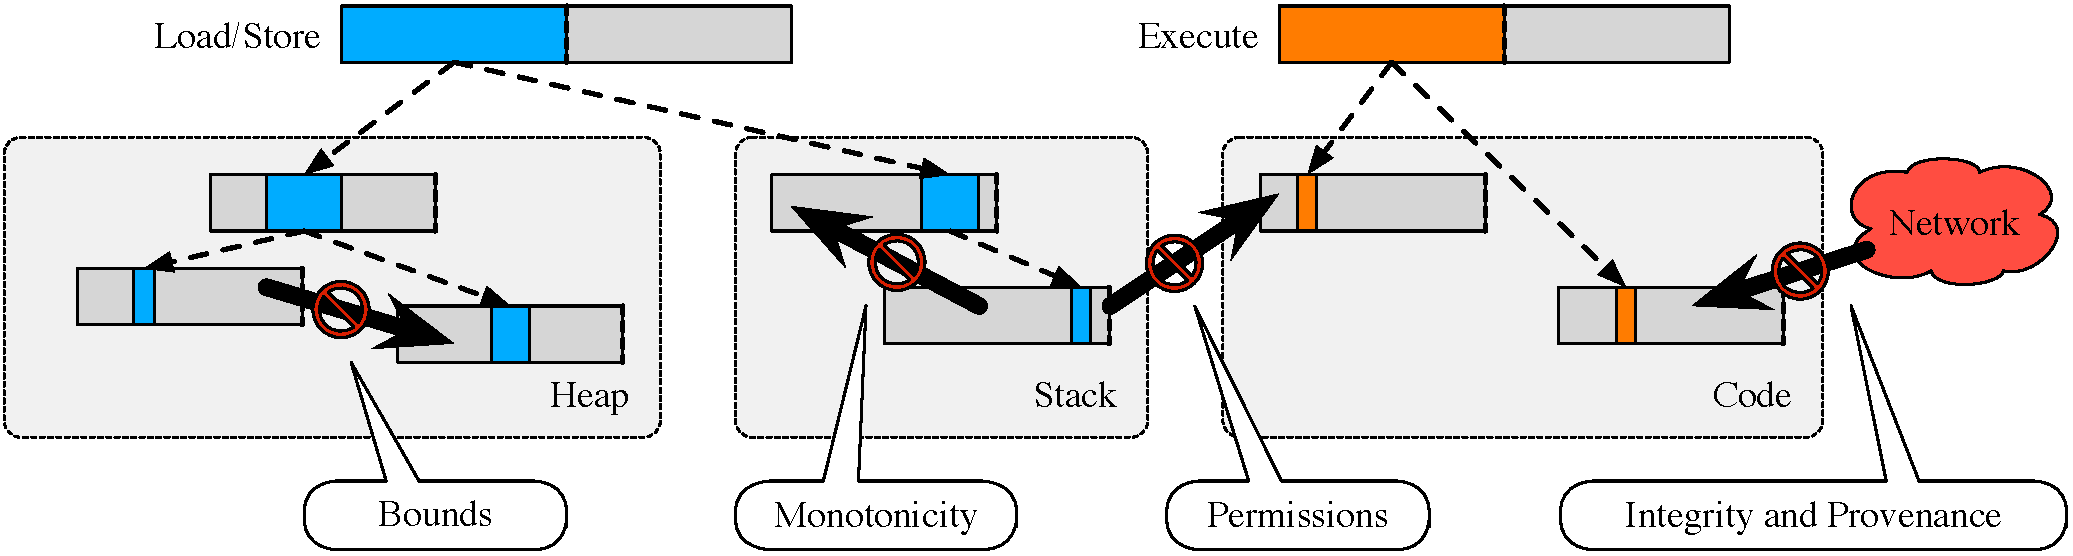
\includegraphics[width=\columnwidth]{fig-pointer-provenance.pdf}
\caption{CHERI enforces strict \textit{integrity}, \textit{provenance
validity}, \textit{monotonicity}, \textit{bounds}, \textit{permissions}, and
\textit{encapsulation} on pointers, mitigating common vulnerabilities and
exploit techniques.}
\label{fig:fig-pointer-provenance}
\end{figure}

In current systems, software typically implements pointers as integer values
stored in two architectural forms: in integer registers, and in memory.
\textit{Architectural capabilities} are a new architectural data type likewise
stored in register and memory, and containing an integer value that will most
frequently be interpreted as an address.
Capabilities also contain a number of other fields that contain additional
metadata associated with the address, such as bounds and permissions, as well
as a tag protecting their integrity.
Compilers, toolchains, and runtimes implementing pointers in terms of
architectural capabilities can imbue pointers with those protections, enforced
in hardware, subject to appropriately managing that metadata.
Capabilities are 2$\times$ (plus 1 bit) the size of the architecture's
natural address size, with the metadata compressed to fit in the additional
space.
On 32-bit architectures, capabilities are 64 bits ($+$1 tag bit), and on
64-bit architectures, capabilities are 128 bits ($+$1 tag bit).
In many senses, architectural capabilities used to implement pointers act like
the integers they replace, being loaded or stored, loaded or stored via,
jumped to, and so on.
The operating system, compiler, linker, and language runtimes are able to use
them to implement fine-grained memory safety for C and C++, as well as for
other purposes such as in-address-space software compartmentalization.

The majority of the capability is stored in a register or in
addressable memory, as is the case
for current integer pointers, with additional metadata stored adjacent to the
integer address it protects.
However, there is also a 1-bit tag that may be
inspected via the instruction set, but is not visible via byte-wise loads and
stores.
This tag is used to record whether the capability is valid; it is
preserved by legal capability operations but cleared by other architectural
operations on that memory.
%
Some of CHERI's protections are for pointers themselves (e.g., their integrity
and provenance validity), whereas others are for the pointee data or code
referenced by pointers (e.g., bounds and permissions).
CHERI's sealing feature protects both a pointer (via immutability) and the
pointee (via non-dereferenceability).

Extending architectures with capability registers and suitable memory storage
naturally aligns with many current architectural and microarchitectural design
choices, as well as software-facing considerations such as compiler code
generation, stack layout, operating-system behavior, and so on.
However, the generalized CHERI protection model can be mapped into
architectures in many different forms.
While implementation choices will affect a variety of factors in the
architecture and microarchitecture, the resulting protection model can be
considered \textit{portable} in that common protection properties and usage
patterns can be mapped into various architectural instantiations.
These topics are considered further in Chapter~\ref{chap:architecture}.

In the remainder of this section, we describe the high-level protection
properties and other functionality that capabilities grant to pointers and
the execution environment (see Figure~\ref{fig:fig-pointer-provenance}):

\begin{itemize}
\item Capability tags for pointer integrity and provenance
  (Section~\ref{sec:model-tags})
\item Capability bounds to limit the dereferenceable range of a pointer
  (Section~\ref{sec:model-bounds})
\item Capability permissions to limit the use of a pointer
  (Section~\ref{sec:model-permissions})
\item Capability monotonicity and guarded manipulation to prevent privilege
  escalation (Section~\ref{sec:model-monotonicity})
\item Capability sealing to implement software encapsulation
  (Section~\ref{sec:model-sealedcapabilities})
\item Capability object types to enable a software object-capability model
  (Section~\ref{sec:model-object-types})
\item Sealed capability invocation to implement non-monotonic domain
  transition (Section~\ref{sec:model-sealed-capability-invocation})
\item Capability control flow to limit pointer propagation
  (Section~\ref{sec:model-capability-control-flow})
\item Capability compression to reduce the in-memory overhead of pointer
  metadata (Section~\ref{sec:model-compression})
\item Hybridization with integer pointers
  (Section~\ref{sec:model-hybridization-integer-pointers})
\item Hybridization with MMU-based virtual memory
  (Section~\ref{sec:model-hybridization-virtual-addressing})
\item Hybridization with ring-based privilege
  (Section~\ref{sec:model-hybridization-architectural-privilege})
\item Failure modes and exception delivery
  (Section~\ref{sec:failuremodesandexceptions})
\item Capability revocation (Section~\ref{sec:model-capability-revocation})
\end{itemize}

\noindent
These features allow capabilities to be architectural primitives upon which
higher-level software protection and security models can be constructed (see
Section~\ref{sec:software-protection-using-cheri}).

\psnote{ perhaps the following subsections should be restructured to
 partition the description of what a capability comprises -- currently
 \ref{sec:model-tags}--\ref{sec:model-permissions} are basically doing
 that, though object types come later -- from the description of
 properties, which currently \ref{sec:model-monotonicity} onwards
 mostly are?   Or, if not, at least have a short bit here that briefly
 says what the data of a capability is.   Perhaps also with an
 \emph{illustrative} bit layout, emphasising that different arch
 instantiations will do things differently.  Could be a bit more
 specific about the permissions data, too.}

\subsection{Tags for Pointer Integrity and Provenance}
\label{sec:model-tags}

Each location that can hold a capability -- whether a capability register or a
capability-sized, capability-aligned word of memory -- has an associated 1-bit
tag that consistently and atomically tracks capability validity for the value
stored at that location:

\begin{description}
\item[Capability registers] each have a 1-bit tag tracking whether the
  in-register value is a valid capability.
  This bit will be set or cleared only as permitted by guarded manipulation.

\item[Capability-sized, capability-aligned words of memory] each have a 1-bit
  tag associated with the location, which is not directly addressable via data
  loads or stores: \textit{tagged memory}.
  Depending on the ISA variant, this may be at 64-bit or 128-bit granularity.
  The capability's address, as well as its other metadata such as
  bounds and permissions, are stored within the capability in addressable
  memory; these fields are protected by the corresponding unaddressable tag
  bit.
  If untagged memory exists in the system, the tags of capability values
  stored to those locations are discarded, and all loaded capability values
  will have the tag bit unset.
\end{description}

\noindent
Tags atomically follow capabilities into and out of capability registers when
their values are loaded from, or stored to, tagged memory.
Stores of other non-capability types -- e.g., of bytes or half words --
automatically and atomically clear the tag in the destination memory location.
This allows in-memory pointer corruption by data stores to be detected on next
attempted dereference -- for example, this prevents arbitrary data received
over the network from being directly dereferenced as a pointer.

The capability tag controls which operations can be performed using a
capability.
Attempting controlled operations on an untagged capability will cause a
precise exception.

Regardless of the value of the tag bit, capability register fields can be
accessed: they can be extracted and, subject to guarded manipulation,
modified.
Similarly, addressable portions of the capability can be read from memory
using ordinary data load and store instructions.
Capability values can also be loaded and stored via other valid capabilities
regardless of the validity of the loaded or stored capability.
An untagged capability value is simply data: allowing capability registers to
hold untagged values allows them to be used for capability-oblivious
operations.
For example, a region of memory can be copied via capability registers, including pointers within data structures, preserving the value of the
tag bit for each copied location.

However, other operations that \textit{dereference} or otherwise use a
capability require that the capability have its tag set -- i.e., be a
\textit{valid capability}.
Dereferencing refers to using the capability to load or store data or other
capabilities, or to fetch instructions.
This includes the implied dereference associated with the Default Data
Capability controlling legacy integer-relative loads and stores.
A valid tag is also required to use a capability to seal or unseal another
capability, to jump to that capability, to use it to set the architectural
compartment ID, or to call it for the purposes of domain transition.
Detailed information on which instructions require capabilities to have valid
tags, or operate on untagged capability values, may be found in the
instruction reference.

Valid capabilities can be constructed only by deriving them from existing
valid capabilities, which ensures \textit{pointer provenance}
(Figure~\ref{fig:fig-pointer-provenance}).
In almost all cases, a new capability value will be derived from a single
capability value -- e.g., as a result of reducing bounds or permissions.
In a few cases, a capability may derive from multiple other capability
values.
For example, a sealed capability is derived from both the authorizing sealing
capability and an original data capability.
Similarly, an explicitly unsealed capability is derived from both the sealed
capability and the capability that authorizes its unsealing.

Implementing C pointers as tagged capabilities allows them to be reliably
identified in the address space, which can help support techniques
such as garbage collection.

Our CHERI 
prototypes implement tagged memory using partitioned memory, with tags and
associated capability-sized units linked close to the memory controller, and
propagated by the cache hierarchy in order to provide strong atomicity with
the data it protects.
However, it is also possible to imagine implementations in which DRAM --
e.g., alongside ECC metadata -- or
non-volatile memory is extended to store tags with capability-sized units as
well.
We similarly assume that DMA will clear tags when writing to memory, although
it is possible to imagine future DMA implementations that are able to
propagate tags (e.g., to maintain tags on capabilities in descriptor rings).

\subsection{Bounds on Capabilities}
\label{sec:model-bounds}

Capabilities contain lower and upper bounds for the memory they authorize
access to.
While a capability's address may move out of bounds (and perhaps back in
again), attempts to dereference (e.g., via a load, store, or instruction
fetch) an out-of-bounds capability will throw a hardware exception.
This prevents exploitation of buffer overflows on global variables, the heap,
and the stack, as well as out-of-bounds execution.
Allowing addresses to sometimes be out-of-bounds with respect to their
bounds -- without faulting -- is important for de-facto C-language
compatibility.
In an ideal world, addresses could be arbitrarily out of bounds.
However, our
bounds-compression scheme places restrictions on this property, as bounds
compression depends on redundancy between the address and bounds, which is
reduced when addresses are substantially outside of their bounds (see
Section~\ref{compression} for details).

Bounds originate in allocation and linking events.
The operating system is able to place bounds on pointers to initial
address-space
allocations during process startup (e.g., via the initial register file, and
ELF auxiliary arguments in memory), and on an ongoing basis as new address-space
mappings are made available (e.g., via \ccode{mmap} system calls).
In practice, most bounds originate in the userspace language runtime or
compiler-generated
code, including the run-time linker for function pointers and global data,
the heap allocator for pointers to heap allocations, and generated code for
pointers taken to stack allocations.
 Programming languages may also offer explicit subsetting support to allow
software to impose its own expectations on suitable bounds for memory accesses
to complex objects (such as in-memory video streams) or in their own memory
allocators.

\subsection{Permissions on Capabilities}
\label{sec:model-permissions}
Capabilities additionally extend addresses with a permissions mask controlling how the
capability may be used.
For example, the run-time linker or compiler may set a capability's
permissions so that pointers to data cannot be reused for instruction fetch,
or so that pointers to code cannot be used to store data.
Further permissions control the ability to load and store capabilities
themselves, allowing the compiler to implement policies such as 
\textit{dereferenceable code and data pointers cannot be loaded from character
strings.}
Permissions can also be made accessible to higher-level aspects of the
run-time and programmer model, offering dynamic enforcement of concepts
similar to \ccode{const}.\footnote{The C-language \ccode{const} qualifier
conflates several orthogonal properties and thus can not be enforced
automatically.
Our language extensions include more constrained \ccode{\_\_input} and
\ccode{\_\_output} qualifiers.}
Languages may provide further facilities to allow programmer-directed
refinement of permissions -- for example, for use in Just-in-Time (JIT)
compilers.

Permissions changes, as with bounds setting, are often linked to allocation
events.
Permissions on capabilities for initial memory memory mappings can be
introduced by the kernel during process startup; further capabilities returned
for new mappings will also have their permissions restricted based on intended
use.
Executable capabilities representing function pointers and return addresses
will be refined by the run-time linker.
Read-only and read-write capabilities referring to data will be refined by the
run-time linker, heap allocator, and stack allocator.

Permissions also control access to the sealing facility used for encapsulation
(see Section~\ref{sec:model-sealedcapabilities}).
While sealing permission could be granted with all data and code capabilities,
best practice in privilege minimization suggests that a separate hierarchy
of sealing pointers should be maintained instead.
Returning independent sealing capabilities via a dedicated system-call
interface reduces opportunities for arbitrary code and data capabilities being
used improperly for this purpose.

\subsection{Capability Monotonicity via Guarded Manipulation}
\label{sec:model-monotonicity}

\textit{Capability monotonicity} is a property of the CHERI protection model
ensuring that new capabilities must be derived
from existing capabilities only via valid manipulations that may narrow (but
never broaden) rights ascribed to the original capability.
This property prevents broadening the bounds on pointers, increasing the
permissions on pointers, and so on, eliminating many manipulation attacks and
inappropriate pointer reuses.
Monotonicity also underlies effective isolation for software
compartmentalization by ensuring that delegated capabilities cannot be used to
reach other resources despite further manipulation.
CHERI enforces capability monotonicity via four mechanisms:

%across the vast majority of its
%instructions\psnote{what does ``vast majority'' mean here?  that it
%  doesn't enforce c.m. for some instructions, or that for some it
%  isn't by g.m., or what?}
%\knnote{The sealedness of a capability is not monotonic, but the
%  bounds and permissions of a capability are monotonic. To avoid
%  defining what ``vast majority'' means, \textit{capability
%    monotonicity} could also be replaced by \textit{capability bounds
%    monotonicity} and \textit{capability permission monotonicity}.}
%by 
%\psnote{think we can just delete this: ``virtue of \textit{guarded manipulation}: they cannot
%represent non-monotonic transformations.
%This is accomplished via''.  I don't see a need to introduce the
%``guarded manipulation'' concept, esp. if we're immediately
%eliminating it, and I don't know exactly what it means.}
% four mechanisms:

\begin{description}
\item[Limited expressivity] Some instructions are prevented, by design, from
  expressing an increase of rights due to the expression of their operands and
  implementation.
  For example, permissions on capabilities are modified using a bitwise `and'
  operation, and hence cannot express an increase in permissions.

\item[Exceptions on monotonicity violation] Some instructions are able to
  represent non-monotonic operations, but attempts to use them
  non-monotonically will lead to an exception being delivered.
  For example, an attempt to broaden bounds on a capability might throw an
  exception without writing back the non-monotonically modified capability.
  Throwing an exception at the point of violation may ease debugging close to
  the point of violation.

\item[Stripping the tag in register write-back] As an alternative to throwing
  an exception, a non-monotonic operation might succeed in writing back a new
  capability -- but with the tag bit cleared, preventing future dereference.
  Clearing the tag allows the failure to be discovered by an explicit
  software check, or on the next attempt to dereference.
  This may make debugging more expensive (if additional checks are introduced,
  perhaps with help from the compiler) or more tricky (if loss of the tag is
  only discovered substantially later).

\item[Stripping the tag in memory store] Tagged memory ensures that direct
  modification of capabilities stored in memory using data store instructions
  (whether non-monotonically or otherwise) will clear the tag on affected
  in-memory capabilities.
  This causes later attempts to dereference the capability to fail.
  This ensures that attempts to modify capabilities cannot bypass guarded
  manipulation.
\psnote{Add an analogous comment about debugging in this situation?
Are all such tag-clears indicative of bugs?  (not necessarily, given
strong updates, but perhaps).    Further to the
CHERI-as-perfect-sanitizer pitch, could we get eager detection here too,
by some combination of h/w and compiler support?}
\rwnote{No -- we frequently overwrite tagged values when storing a NULL,
  initialising memory, writing via another type in a union, doing a COW onto
  a page, etc.  There are surely cases where clearing the tag is a bug, but
  I suspect most cases are not.}

\end{description}

Selecting which enforcement mechanism to use will reflect the specific
operation being implemented, concerns about about ease of debugging, as well
as the context of the surrounding architecture. For example, in some
architectures, exceptions can be thrown on any instruction (e.g., MIPS), while
in others it is preferable for exceptions to be thrown only on memory
accesses (e.g., ARMv8-A).
As a result of these combined architectural features, guarded manipulation
implements \textit{non-bypassable capability monotonicity}.
\knnote{I don't know what ``non-bypassable'' means here: if the
  sentence would read ``\ldots implements capability monotonicity''
  would that already be enough? I also wonder whether this sentence
  should repeat that capabilities are not always monotonic.}

Monotonicity allows reasoning about the set of reachable rights for executing
code, as they are limited to the rights in any capability registers, and
inductively, the set of any rights reachable from those capabilities -- but no
other rights, which would require a violation of monotonicity.
\knnote{But CHERI does violate monotonicity. Perhaps it would help to
  introduce the exceptions to monotonicity first, and then discuss in
  this paragraph why these exceptions are not a problem for
  compartmentalization.}
Monotonicity is a key foundation for fine-grained compartmentalization, as it
prevents delegated rights from being used to gain access to other undelegated
areas of memory.
More broadly, monotonicity contributes to the implementation of the principle
of intentional use, in that capabilities not only cannot be used for
operations beyond those for which they are authorized, but also cannot
inadvertently be converted into capabilities describing more broad rights.

The two notable exceptions to strict monotonicity
\psnote{are these really exceptions to c.m. in the specific sense
  defined above, about the construction of new capabilities?   They
  have more to do with the lack of monotonicity of the permissions of
  the current hardware thread...}
 are invocation of sealed
capabilities (see Section~\ref{sec:model-sealed-capability-invocation}) and
exception delivery (see Section~\ref{sec:failuremodesandexceptions}).
\knnote{Is unsealing capabilities with \textit{CUnseal} an exception to monotonicity?}
Where non-monotonicity is present, control is transferred to code trusted to
utilize a gain in rights appropriately -- for example, a trusted
message-passing routine in the userspace runtime, or an OS-provided exception
handler.
This non-monotonicity is required to support protection-domain transition from
one domain holding a limited set of rights to destination domain that holds
rights unavailable to the originating domain -- and is therefore also
a requirement for fine-grained compartmentalization (see
Section~\ref{sec:model-isolation-controlled-communication-compartmentalization}).


\subsection{Capability Flags}
\label{sec:model-flags}
Capabilities include a flags field that can be manipulated freely.
Unlike the permissions field, it does not determine privilege, i.e., the state
of this field is orthogonal to capability monotonicity.
%
That is, these flags are intended to affect the \emph{semantics} of access,
rather than impose access control.
%
Currently, there are only architecture-specific interpretations for this
field: CHERI-RISC-V uses it to control opcode interpretation on instruction
fetch.
In the future, other non-security behavioral flags relating to capabilities may
be placed here, such
as to hint as to cache interactions for shared-memory rings, or to control
the behavior of operations such as capability equality testing.

\subsection{Sealed Capabilities}
\label{sec:model-sealedcapabilities}

Capability \textit{sealing} allows capabilities to be marked as
\textit{immutable} and \textit{non-deref\-erenceable}, causing hardware
exceptions to be thrown if attempts are made to modify, dereference, or jump
to them.
This enables capabilities to be used as unforgeable tokens of authority for
higher-level software constructs grounded in \textit{encapsulation}, while
still allowing them to fit within the pointer-centric framework offered by CHERI
capabilities.
There are two forms of capability sealing: pairs of capabilities sealed
using a common \textit{object type}, and stand-alone \textit{sealed entry
capabilities} (sentry capabilities).

Sealed pairs are primarily designed to support the linking of a pair of code
and data capabilities for use together during domain transition.
A jump-like instruction, \insnref{CInvoke}, allows the two sealed
capabilities to be atomically unsealed as control flow transfers to the code
pointed to by the code capability, if their object types match.
This can be used to implement controlled privilege escalation for the purposes
of domain transition.

Sealed entry capabilities simply seal a single code capability, which likewise
can be jumped to leading to an atomic unsealing and control-flow transfer.
This can also be used to implement domain transition with privilege
escalation, but to date has primarily been used to strengthen control-flow
robustness within a single protection domain by preventing the undesired
manipulation and use of code pointers.
Jump-and-link instructions acting on sealed entry capabilities also generate
a sealed return capability.

Sealed capabilities can also be used to support other operating-system or
language robustness features, such as representing other sorts of delegated
(non-hardware-defined) rights, or ensuring that pointers are dereferenced only
by suitable code (e.g., in support of language-level memory or type safety).

\rwnote{The next few subsections feel a bit redundant, and could be
  condensed.}

\subsection{Capability Object Types}
\label{sec:model-object-types}

Capabilities contain an additional piece of metadata, an \textit{object
type}\psnote{that sounds as if \emph{all} capabilities contain an
  object type...}%
\nwfnote{They do, at least implicitly!  \insnref{CGetType} returns
something, specifically $2^{64}-1$, for unsealed capabilities.  I've tried
to make the ISA speak in terms of \emph{encoding} the architectural
\cotype{} into the bit patterns of a capability, rather than being exactly
those bits, so that we can uniformly treat CC's separate \cotype{} field
and C-128's \csealed{} flag and shared \cotype{} bits.}%
, updated when a capability undergoes (un)sealing.
Object types allow multiple sealed capabilities to be indelibly (and
indivisibly) linked, so that the kernel or language runtime can avoid
expensive checks (e.g., via table lookups) to confirm that they are intended
to be used together.
%
\nwfnote{I am not sure I like ``indivisibly'' or maybe ``linked'' above; the indivisibility is
only up to ${\sim}/\cotype{}$, but it almost sounds like it's specifically a
pair of capabilities that are linked.  Perhaps ``associated''?}
%
For example, for object-oriented compartmentalization models,
pairs of sealed capabilities can represent
objects: one is the code capability for a class, and the other is a data
capability representing the data associated with a particular instance of an
object.

The object-type field is set when a capability is sealed based on a second
input capability authorizing use of the type space -- itself simply a
capability permission authorizing sealing within a range of values specified
by the capability's bounds.
A similar model authorizes \textit{unsealing}, which permits a sealed
capability to be restored to a mutable and dereferenceable state -- if a
suitable capability to have sealed it is held.

A similar model could be achieved without using an unsealing mechanism: a
suitably privileged component could inspect a sealed capability and rederive
its unsealed contents.
However, authorizing both sealing and unsealing based on type capabilities
allows the right to construct encapsulated pointers to be delegated, without
requiring recourse to a privileged software supervisor at the cost of
additional domain transitions -- or exercise of unnecessary privilege.

\subsection{Sealed Capability Invocation}
\label{sec:model-sealed-capability-invocation}

CHERI supports two forms of non-monotonicity\psnote{someone should
  revisit this phrasing after the glossary for monotonicity is sorted
  out: either that is only up to domain transitions, in which case
  these aren't non-..., or not, in which case these are}: jump-like capability invocation,
and exception handling (see Section~\ref{sec:failuremodesandexceptions}).
The \insnref{CInvoke} instruction accepts a pair of sealed
capability operands on which various checks are performed (for example, that
they are valid, sealed, and have matching object types).
If all tests are passed, then additional capabilities become available to the
executing CPU context by virtue of unsealing of the operand
registers.

The destination execution environment has well-defined and
reliable properties, such as a controlled target program-counter capability
and additional data capability that can be used to authorize domain
transition.
\insnref{CInvoke} behaves much like a conventional jump to register, permitting an
in-address-space domain switch without changing rings.

The newly executing code has the ability to further manipulate
execution state, and impose semantics such as call-return secure function
invocation or secure asynchronous message passing,
which will likely be followed by a privilege de-escalation as a target domain
is entered (see
Section~\ref{sec:model-isolation-controlled-communication-compartmentalization}).

\subsubsection{Object-Capability Policies in CHERI}

Consider an execution environment having access to several capabilities
sealed with the same \texttt{otype}.  The tests required by the
\insnref{CInvoke} mechanism describe a \emph{Cartesian product} of method
rights (indicated by the sealed code capability) and object rights (sealed data
capability) to this environment.  Regardless of how the environment
came to have these sealed capabilities, it is free to pair any sealed code
capability with any sealed data capability and have the \insnref{CInvoke}
tests pass.

Non-Cartesian and/or stateful policies can be encoded by
indirection, using memory to store additional data to be checked by the
invoked subsystem on entry.  The sealed data pointers given out by the
invoked subsystem now no longer directly reference objects; instead, they
reference ``data trampolines'' describing the pairing of object(s) \emph{and
remote agent(s)} with associated access rights information.  Attenuation of
access rights is no longer necessarily an ambiently available action and
requires either the explicit construction of membranes (i.e., proxy objects)
or active cooperation of the invoked subsystem (or an agent acting on its
behalf) to create new data trampoline(s).

\subsection{Capability Protection for Non-Pointer Types}

While the design of CHERI capabilities is primarily focused on the protection
of pointers, the pointer interpretation of capabilities depends entirely on
a capability's permissions mask.
If the mask authorizes load, store, and fetch instructions, then the
capability has a pointer interpretation.
\psnote{recent discussion in WG14/21 makes me sensitive to this:
  there's important code out there that relies on equality comparison
  of pointers to objects after lifetime-end of those objects, and the
  analogue of that in CHERI (with some temporal safety scheme) could
  be capabilities with tags or permissions cleared -- in which case
  they'd still have \emph{a} pointer interpretation, albeit a limited one}
Capabilities are not required to have those permissions set, however, allowing
capabilities to be used for other purposes -- for example, to protect other
critical data types from in-memory corruption (such as implementing UNIX file
descriptors or stack canaries), or to authorize access to system services
(such as authorizing use of specific system calls identified by the
capability).
Sealed capabilities and a set of software-defined permissions bits facilitate
these use cases by permitting non-architecture-defined capability
interpretations while retaining capability-based protections.

\subsection{Capability Flow Control}
\label{sec:model-capability-control-flow}

The CHERI capability model is designed to support the implementation of
language-level pointers: tagged memory allows capabilities to be stored in
memory, and in particular, embedded within software-managed data structures
such as objects or the stack.
CHERI is therefore particularly subject to a historic criticism of
capability-system models -- namely,
that capability propagation makes it difficult to track
down and revoke rights (or to garbage collect them).
To address this concern, CHERI has three mechanisms by which the flow of
capabilities can be constrained:

\begin{description}

\item[Capability PTE bits] extend the existing load and store
  permissions on page-table entries with new permissions to authorize loading and storing
  of capabilities.
  This allows the operating system to maintain pages from which tagged
  capabilities cannot be loaded (tags will be transparently stripped on load),
  and to which capabilities cannot be stored (a hardware exception will be
  thrown).
  This can be used, for example, to prevent tagged capabilities from being
  stored in memory-mapped file pages (as the underlying object might not
  support tag storage), or to create regions of shared memory through which
  capabilities cannot flow.

\item[Capability load and store permission bits] extend the load and store
  permissions on capabilities themselves, similarly allowing a capability to
  be used only for data access -- if suitably configured.
  This can be used to create regions of shared memory within an address
  space through which capabilities cannot flow.
  For example, it can 
prevent
  two separated compartments from
  delegating access to one another's memory regions, instead limiting
  communication to data traffic via the single shared region.
%%%% THE ORIGINAL SENTENCE WAS CONVOLUTED, ALLOWING SOMETHING NOT TO HAPPEN
%%%% DID NOT MAKE ANY SENSE.  ON THE OTHER HAND, I MAY HAVE GOTTEN THE FIX
%%%% BACKWARDS!

\item[Capability control-flow permissions] ``color'' capabilities to limit
  propagation of specific types of capabilities via other capabilities.
  This feature marks capabilities as \textit{global} or \textit{local} to
  indicate how they can be propagated.
  Global capabilities can be stored via any capability authorized for
  capability store.
  Local capabilities can be stored only via a capability specifically
  authorized as \textit{store local}.
  This can be used, for example, to prevent propagation of temporally
  sensitive stack memory between compartments, while still allowing
  garbage-collected heap memory references to be shared.

  This feature remains under development, as we hope to generalize it to
  further uses such as limiting the propagation of ephemeral DRAM references
  in persistent-memory systems.

\end{description}

The decision to strip tags on load, but throw an exception on
store\psnote{this might be rather opaque to readers -- did it refer to
  text that isn't there any more?  maybe expand to
explain?}, reflects
pragmatic software utilization goals: language runtimes and system libraries
often need to implement \textit{capability-oblivious memory copying}, as the
programmer may not wish to specify whether a region of memory must (or must
not) contain capabilities.
By stripping tags rather than throwing an exception on load, a
capability-oblivious memory copy is safe to use against arbitrary
addresses and source capabilities -- without risk of throwing an exception.
Software that wishes to copy only data from a source capability (excluding tag
bits due to a non-propagation goal) can simply remove the load-capability
permission from the source capability before beginning a memory copy.
%%%% THIS only SEEMS TO BE IN THE RIGHT PLACE: only specific data,
%%%% RATHER THAN data only from a source capability!!! 

On the other hand, it is often desirable to detect stripping of a capability on
store\psnote{this may also appear cryptic} via a hardware exception, to ease debugging.
For example, it is typically desirable to catch storing a tagged capability to
a file as early as possible in order to avoid debugging a later failed
dereference due to loss of a tag.
Similarly, storing a tagged capability to a virtual-memory page might be an
indicator to a garbage collector that it may now be necessary to scan that
page in search of capabilities.

This design point conserves PTE and permission bits; there is some argument
that completing the space (i.e., shifting to three or four bits
each\psnote{each what?}) would
offer functional improvements -- for example, the ability to avoid exceptions on
a capability-oblivious memory copy via a capability that does not authorize
capability store, or the ability to transparently strip tags on store to a
shared memory page.
However, we have not yet found these particular combinations valuable in our software experimentation, 

\subsection{Capability Compression}
\label{sec:model-compression}

\psnote{confusing contrast between ``in-memory representation'' and
  ``implementation'' -- I suspect better to position these as
  architectural alternates, rather than the latter as an
  ``implementation'' of the former}
\psnote{I suspect there needs to be some clarification across the
  whole document about whether ``128-bit'' refers to the old 128-bit
  scheme, or CHERI concentrate, or both? (and some particular version
  of concentrate?)}

Architecturally, capability fields are exposed via a set of accessor
instructions that get or set field values, such as the address, upper bound,
lower bound, and permissions.
The in-register and in-memory formats for capability contents may differ
substantially, permitting a more efficient representation using compressed
capability bounds.
CHERI utilizes a floating-point-like \textit{fat-pointer compression
technique} that relies on redundancy between the address, lower bound, and
upper bound.
The compressed representation exchanges stronger alignment requirements
(proportional to object size) for a more compact representation.

The CHERI Concentrate compression model (see Section~\ref{compression}) maintains monotonicity:
no ISA manipulation of a
capability can grant increased rights, and when unrepresentable cases are
generated
(e.g., a pointer substantially out of bounds, or a very unaligned object),
the pointer becomes un-dereferenceable.
Memory allocators already implement alignment requirements for heap and stack
allocations (word, pointer, page, and superpage alignments), and these
algorithms require only minor extension to ensure fully accurate bounds for
large memory allocations. Small allocations require no additional
alignment, where the definition of `small' depends on the compression format used and might be from 4 kiB to 1 MiB.
Relative to a 64-bit pointer, the 128-bit design reduces per-pointer memory
overhead (with a strong influence on cache footprint for some software
designs) by roughly two thirds, compared to, for example, a 256-bit
representation as found in earlier CHERI versions.

\subsection{Hybridization with Integer Pointers}
\label{sec:model-hybridization-integer-pointers}

Processors implementing CHERI capabilities also support existing programs
compiled to use conventional integer pointers, rather than capability
pointers, using two special capability registers:

\begin{description}
\item[Default Data Capability (DDC)] DDC indirects and controls legacy
  instructions that load and store relative to integer addresses rather than
  capabilities.

\item[Program Counter Capability (PCC)] PCC extends the conventional program
  counter with capability metadata, indirecting and controlling instruction
  fetches.
\end{description}

Programs compiled to use capabilities to represent pointers (whether
implicitly or via explicit program annotations) will not use the default data
capability, instead employing capability registers and capability-based
instructions for pointer operations and indirection.
The program-counter capability will be used regardless of the code model
employed, although capability-aware code generation will employ constrained
program-counter bounds and permissions to implement control-flow robustness
rather than using a single large code segment.
Support for legacy loads and stores can be disabled by installing a
sufficiently constrained (e.g., untagged) default data capability.

Different compilation modes and ABIs provide differing levels of compatibility
with existing code -- but include the ability to run entirely unmodified
non-CHERI binaries, to execute non-CHERI code in sandboxes within CHERI-aware
applications, and CHERI-aware code in sandboxes within CHERI-unaware
applications.

\subsection{Hybridization with Virtual Addressing}
\label{sec:model-hybridization-virtual-addressing}

\begin{figure}[t]
\centering
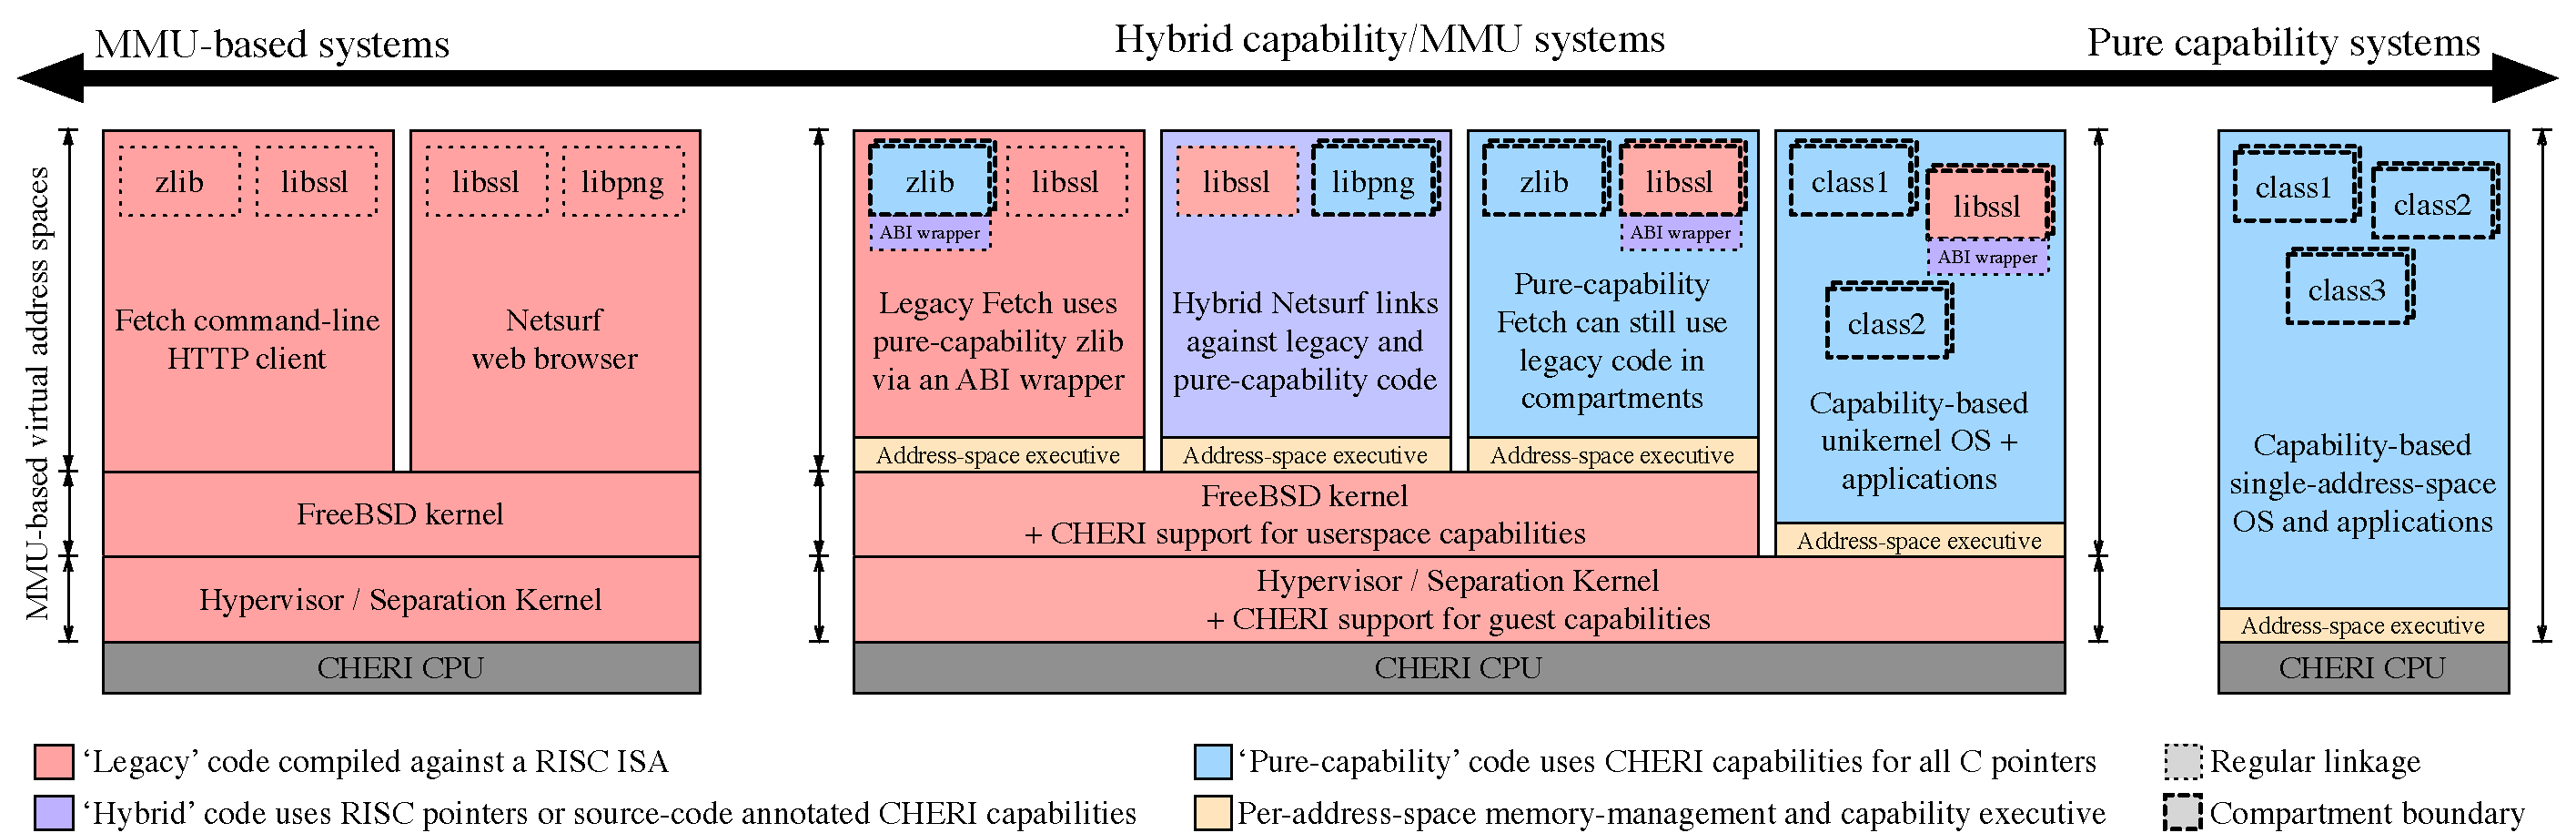
\includegraphics[width=\columnwidth]{fig-cheri-high-level.pdf}
\caption{CHERI supports a wide range of operational software models including:
unmodified MMU-based operating systems; hybrid operating systems
utilizing the MMU to support a process model and/or virtualization while
using CHERI within virtual address spaces; and pure single-address-space
CHERI-based operating systems.}
\label{fig:fig-os-models}
\end{figure}

The above features\psnote{which? just those in the preceding
  subsection, or all in this chapter?} compose naturally with, and complement, the Virtual-Memory (VM)
models commonly implemented using commodity Memory Management Units (MMUs) in
current OS designs (Figure~\ref{fig:fig-os-models}).
Capabilities are \textit{within} rather than \textit{between} address spaces;
they protect programmer references to data (pointers), and are intended to be
driven primarily by the compiler rather than by the operating system.
In-address-space compartmentalization complements process isolation by
providing fine-grained memory sharing and highly efficient domain switching
for use between compartments in the same application, rather than between
independent programs via the process model.
Operating-system kernels will also be able to use capabilities to improve the
safety of their access to user memory, as user pointers cannot be accidentally
used to reference kernel memory, or accidentally access memory outside of
user-provided buffers.
Finally, the operating system might choose to employ capabilities internally,
and even in its interactions with userspace, in referencing kernel data
structures and objects.

\subsection{Hybridization with Architectural Privilege}
\label{sec:model-hybridization-architectural-privilege}

Conventional architectures employ ring-based mechanisms to control use of
architectural privilege: only code executing in ``supervisor'' or ``kernel''
mode is permitted to access the virtual address space with supervisor rights,
but also to control the MMU, certain cache management operations,
interrupt-related features, system-call return, and so on.
The ring model prevents unprivileged code from manipulating the virtual
address space (and other processor features) in such a way as to bypass memory
protection and isolation configured by the operating system.
Contemporary instantiations may also permit virtualization of those features,
allowing unmodified operating systems to execute efficiently over microkernels
or hypervisors.
CHERI retains support for these models with one substantial modification: use
of privileged features within privileged rings, other than in accessing
virtual memory as the supervisor, depends on the program-counter capability
having a suitable hardware permission set.

This feature similarly allows code \emph{within} kernels, microkernels, and
hypervisors to be compartmentalized, preventing bypass of the capability model
within the kernel virtual address space through control of virtual memory
features.
The feature also allows vulnerability mitigation by allowing only explicit
use of privileged features: kernel code can be compiled and linked so that
most code executes with a program-counter capability that does not authorize
use of privilege, and only by jumping to selected program-counter capabilities
can that privilege be exercised, preventing accidental use.
Finally, this feature paves the way for process and object models in which the
capability model is used without recourse to rings.

\subsection{Failure Modes and Exceptions}
\label{sec:failuremodesandexceptions}

Bounds checks, permissions, monotonicity, and other properties of the CHERI
protection model inevitably introduce the possibility of new ISA-visible
failure modes when software violates rules imposed through capabilities
(whether due to accident or malicious intent).
We have selected to deliver failures as \textit{hardware exceptions}; for
example, on attempts to perform disallowed load and store operations, to
broaden bounds, and so on.
This allows the operating system (which in turn may delegate to the userspace
language runtime or application) the ability to catch and handle failures in
various ways -- such as by emulating disallowed accesses, converting to a
language-visible exception, or performing some diagnostic or mitigation
activity.

Different architectures express differing design philosophies for when
exceptions may be delivered, and there is flexibility in the CHERI model in
when exceptions might be delivered.
For example, while an attempt to broaden (rather than narrow) bounds could
generate an immediate exception, the operation could instead generate a
non-dereferenceable pointer as its output, in effect deferring an exception
until the time of an attempted load, store, or instruction fetch.
Both of these implementations ensure monotonicity by preventing derived
pointers from improperly allowing increased access following guarded
manipulation, and are consistent with the model.

Initially, in our prototyping, we selected to deliver exceptions as early as
possible when such events occur.
However, all current CHERI ISA instantiations defer exceptions to the use
of a capability's authority, instead clearing the tag on operations that
would otherwise violate monotonicity.

\pdrnote{The following two paragraphs perhaps belong in rationale?}
The early exception approach offers slightly improved debuggability
(by exposing the error earlier).
However, early exceptions limit compiler optimization as instructions that may
throw exceptions are restricted in how they can safely be reordered.
For example, a bounds restriction performed within a loop could be hoisted to
before the loop, except for the possibility that the bounds are being widened.
In addition, code that manipulates untrusted capabilities is forced to branch
when the operation would be illegal, or risk being vulnerable to
denial-of-service attacks.
This may require it to recreate the hardware-performed checks in software.

With a deferred-exception approach, as well as avoiding these issues,
microarchitecture is simplified by reducing the set of instructions that can
throw exceptions.
While it is initially tempting to delay performing the required checks,
forwarding the common-case value and later flushing the pipeline if a check
fails, this leads to exploitable speculative side channel attacks.
As such, in either approach, microarchitecture must perform the checks
before forwarding the result.
Early exceptions can still be achieved if desired for debugging by
instrumenting potentially tag-clearing instructions with assertions about
the tag, either manually or in a compiler santitization pass.
The CHERI ISA design can ensure these checks are cheap, for example by
providing an instruction to throw an exception based on the tag.

\subsection{Capability Revocation, Garbage Collection, and Flow Control}
\label{sec:model-capability-revocation}

Revocation is a key design concern in capability systems, as revocation is
normally implemented via table indirection -- an approach in tension with the
CHERI design goal of avoiding table-based lookups or indirection on pointer
operations.
As described in Section~\ref{sec:model-capability-control-flow}, CHERI provides
explicit ISA-level features to constrain the flow of capabilities in order to
reduce the potential overhead in walking through memory to find outstanding
capabilities to resources (e.g., to implement garbage collection or sweeping
revocation).
There are also explicit features in the instruction-set architecture that
directly support the implementation of both pointer and object-capability
revocation:

\begin{description}
\item[MMU-based virtual-address revocation]
  As CHERI capabilities are evaluated prior to virtual addressing (i.e., they
  are pointers within address spaces), the MMU can be used not only to
  maintain virtual address spaces, but also to explicitly prevent the
  dereferencing of pointers to virtual address ranges -- regardless of the
  capability mechanism.
  Combined with a policy of either non-reuse of virtual address space (as
  distinct from non-reuse of physical address space), sweeping revocation, or
  garbage collection, this 
  allows all outstanding capabilities (and any further capabilities derived
  from them) to be revoked without the need to search for those capabilities
  in the register file or memory.
  This revocation is subject to the granularity and scalability limitations
  of MMUs: for example, it is not possible to revoke portions of the virtual
  address space smaller than one page.

  This low-level hardware mechanism must be combined with suitable software
  management of the virtual address space in order for it to be effective.
  For example, a policy of non-reuse of the virtual address space at
  allocation time will prevent stale capabilities from referring to a new
  allocation after an old one has been freed.
  A further policy of revoking MMU mappings for the region of virtual address
  space will prevent use of the freed memory as a communications channel from
  the point of free.
  Asynchronous and batched revocations will improve performance, subject to
  windows of opportunity in which use after free (but not use after
  re-allocation) might still be possible.
  It is also worth observing explicitly that non-reuse of the virtual address
  space in no way implies non-reuse of physical memory, as memory underlying
  revoked virtual addresses can be safely reused.
  An alternative to virtual address-space non-reuse is garbage collection, in
  which outstanding references to freed (and perhaps revoked) virtual address
  space are sought and explicitly invalidated.

  Use of the MMU for virtual address-space revocation is subject to a number
  of limits depending on the non-reuse and garbage-collection policies
  adopted.
  For example, if small, sub-page-size, tightly packed memory allocations
  are freed in a manner that leads to fragmentation (i.e., both allocated and
  freed memory within the same virtual page), then revocation will not be
  possible -- as it would prevent access to valid allocations (which could be
  emulated only at great expense).
  Similarly, fragmentation of the virtual address space may lead to greater
  overhead in the OS's virtual-memory subsystem, due to the need to maintain
  many individual small mappings, as well as the possibility of reduced
  opportunity to use superpages should revocations occur that are expressed
  in terms of smaller page sizes.

  However, overall, the MMU provides a non-bypassable means of preventing use
  of all outstanding capabilities to a portion of the virtual address space,
  permitting strong revocation to be used where appropriate.

\item[Accurate garbage collection]
  Traditional implementations of C are not amenable to accurate garbage
  collection because unions and types such as \ccode{intptr_t} allow a register
  or memory location to contain either an integer value or a pointer.
  CHERI-C does not have this limitation: The tag bit makes it possible to
  accurately identify all memory locations that contain data that can be
  interpreted as a pointer.
  Garbage collection is the logical dual of revocation: garbage collection
  extends the lifetime of objects as long as they have valid references, whereas
  revocation curtails the lifetime of references once the objects to which they
  refer are no longer valid.
  A simple stop-the-world mark-and-sweep collector for C can perform both tasks,
  scanning all reachable memory, invalidating all references to revoked objects, and recycling unreachable memory.

  More complex garbage collectors typically rely on read or write barriers
  (i.e., mechanisms for notifying the collector that a reference has been read or
  written).
  These are typically inserted by the compiler; however, in the context of revocation
  the compiler-generated code must be treated as untrusted.
  It may be possible to use the permission bits -- either in capabilities
  themselves or in page-table entries -- to introduce traps that can be used as
  barriers.

\item[Capability tags for sweeping revocation]
  In addition to supporting garbage collection, capability tags in registers
  and memory also allow the reliable identification of capabilities for the
  purposes of explicit revocation.
  Subject to safety in the presence of concurrency (e.g., by suspending
  software execution in the address space, or temporarily limiting
  access to portions of the address space), software can reliably
  sweep through registers and memory, clearing the tags (or otherwise
  replacing)
for
 capabilities that are to be revoked.
  This comes at potentially significant cost, which can be mitigated through
  use of the MMU -- e.g., to prevent capabilities from being used in certain
  pages intended only to store data, or to track where capabilities have been
  stored via a capability dirty bit in virtual-memory metadata.

\item[Revocation of sealed capabilities]
  When the interpretation of sealed capabilities is performed by a trustworthy
  software handler, there is the opportunity for that
  handler to implement revocation semantics explicitly.
  For example, the object invocation handler of a trusted userspace
  supervisor entered by \insnref{CInvoke}
  could interpret the
  address of a sealed capability as pointing to a table entry
  within its domain,
  rather than directly encapsulating a pointer to the target object's data.
  The address could be split into two parts: a table index, and a generation
  counter.
  The table entry could then itself contain a generation counter.
  Sealed object-capability references to the table entry would incorporate
  the value of the counter at the time of sealing, and the invocation handler
  would check the generation count, rejecting invocation on a mismatch.
  When object-capability revocation is desired, the table generation counter
  could be bumped, preventing any further use of outstanding references.
  This approach would be subject to limits on table-entry reuse and the size
  of the table; for example, a reasonable design might employ a 24-bit table
  index (permitting up to $2^{24}$ objects in the system at a time) and a
  40-bit generation counter.
  Use of the 24-bit object-type could further increase the number of objects
  permissible in the system concurrently.
  Many other similar schemes incorporating explicit checks for revocation
  based on software interposition employing counters, tables, etc., can be
  imagined.
\end{description}

CHERI includes several architectural features to facilitate techniques such
as garbage collection and sweeping revocation.
Tags allow capabilities to be accurately identified in both registers and
memory.
In addition, CHERI can limit the flow of capabilities via various mechanisms,
limiting the memory areas that must be swept for the two techniques: MMU
permissions controlling capability load and store via specific pages;
capability permissions controlling capability load and store via specific
capabilities; and the local-global feature that controls the propagation of
subsets of capabilities.
These primitives may be combined to support higher-level software policies
such as:

\begin{itemize}
\item ``capabilities may not be shared between address spaces''
\item ``local stack capabilities may be stored only to the local stack''
\item ``this shared-memory buffer can be used only for data sharing, not
  capability sharing''
\item ``capabilities can flow only one way through this shared buffer''
\item ``only the TCB can introduce capabilities to shared memory between
  compartments''
\item ``supervisor involvement is required to share sealed capabilities
  between compartments''
\item ``first store of a capability to any page will deliver an exception to
  the supervisor''
\end{itemize}

\noindent
As a result, garbage collection and sweeping revocation can rely on strong
invariants about capability propagation that limit the areas of memory that
must be swept for garbage collection or revocation.

\section{Software Protection and Security Using CHERI}
\label{sec:software-protection-using-cheri}

The remainder of the chapter explores these ideas\psnote{which?  just 2.3.16
\emph{Capability Revocation, Garbage Collection, and Flow Control}, or
everything in 2, or the section title?} in greater detail,
describing the high-level semantics
 offered
by the ISA and how they are mapped
into programmer-visible constructs such as C-language features.
The description in this chapter is intended to be agnostic to the specific
Instruction-Set Architecture (ISA) in which CHERI is implemented.  
In particular, it is important that programmers be able to rely on the
properties described in this chapter -- regardless of the ISA-level
implementation -- 
and that software abstractions built over these properties have 
consistent behavior that can be depended upon to mitigate vulnerabilities.

\subsection{Abstract Capabilities}

The CHERI architecture imposes tight constraints on capability manipulation and
use including provenance validity and monotonicity.
While these rules generally permit the execution of current C and C++ code
without significant modification, there are occasions on which the
programmer model of pointer properties (for example) may violate rules for
capabilities.
For example, the architecture maintains provenance validity of capabilities
from reset, permitting them to remain valid only if they are held in tagged
memory or registers.
In practice, operating systems may swap memory pages from DRAM to disk and
back, violating architectural provenance validity.
The OS kernel is able to maintain the appearance of provenance validity for
swapped pages by saving tags when swapping out, and re-deriving capabilities
from valid architectural capabilities when swapped back in -- maintaining the
\textit{abstract capabilities} that compiler-generated code works with.
Our ASPLOS 2019 paper on CheriABI explores this issue in
detail~\cite{davis2019:cheriabi}, covering topics such as context switching,
the C-language runtime, virtual-memory behavior, and debugging.

\subsection{C/C++ Language Support}

CHERI has been designed so that there are clean mappings from the C and C++
programming language into these protection properties.  Unlike
conventional virtual memory, the compiler (and not just the operating system)
is intended to play a significant role in managing these protections.
Protection is within address spaces, whether in a conventional user
process, or within the operating-system kernel itself in implementing its own
services or in accessing user memory:

\begin{description}
\item[Spatial safety]
CHERI protections are intended to directly protect the \textit{spatial safety}
of userspace types and data structures.  This protection includes
the integrity of pointers to code and
data, as well as implied code pointers in the form of return addresses and
vtable entries; bounds on heap and stack allocations; the  prevention
of executable data, and modification of executable code via permission.

\item[Temporal safety]
CHERI provides instruction-set foundations for higher-level \textit{temporal
safety} properties, such as non-reuse of heap allocations via garbage
collection and revocation, and compiler clearing of return addresses on the
stack.
In particular, the capability tags on registers and in memory allows pointers
to be reliably located and atomically replaced with a different value
(including an invalid capability).
Acceleration features allow capabilities to be located more efficiently than
simply sweeping all of physical memory.

\item[Software compartmentalization]
CHERI provides hardware foundations for highly efficient
\textit{software compartmentalization}, the fine-grained decomposition of
larger software packages into 
smaller isolated components that are 
granted access
only to the memory (and also software-defined) resources they actually require.

\item[Enforcing language-level properties]
CHERI's software-defined permission bits and sealing features can also be used
to enforce other language-level protection objectives (e.g., opacity of
pointers exposed outside of their originating modules) or to implement
hardware-assisted type checking for language-level objects (e.g., to more
robustly link C++ objects with their corresponding vtables).

\end{description}

\noindent
CHERI protections are implemented by a blend of 
functionality:

\begin{description}

\item[Compiler and linker] responsible for generating code that manipulates
  and dereferences code and data pointers, compile-time linkage, and 
  stack allocation.

\item[Language runtime] responsible for ensuring that program run-time
  linkage, memory allocation, and exceptions implement suitable policies in
  their refinement and distribution of capabilities to the application and its
  libraries.

\item[Operating-system kernel] responsible for interactions with conventional
  virtual memory, maintaining capability state across context switches,
  reporting protection failures via signals or exceptions, and implementing
  domain-transition features used with compartmentalization.

\item[Application program and libraries] responsible for distributing and
  using pointers, allocating and freeing memory, and employing higher-level
  capability-based protection features such as compartmentalization during
  software execution.

\end{description}

\subsubsection{Data-Pointer Protection}

Depending on 
the desired 
compilation mode, some or all data pointers will be implemented
using capabilities.
We anticipate that memory allocation (whether from the stack or heap, or via
kernel memory mapping) will return capabilities whose bounds and permissions
are suitable for the allocation, which will then be maintained for any derived
pointers, unless explicitly narrowed by software.
This will provide the following general classes of protections:

\begin{description}
\item[Pointer integrity protection] Overwriting a pointer in memory with data
  (e.g., received over a socket) will not be able to construct a
  dereferenceable pointer.

\item[Pointer provenance checking and monotonicity] Pointers must be derived
  from prior pointers via manipulations that cannot increase the range or
  permissions of the pointer.\psnote{TODO: check consistency with
    glossary for provenance after that's updated}

\item[Bounds checking] Pointers cannot be moved outside of their allocated
  range and then be dereferenced for load, store, or instruction fetch.

\item[Permissions checking] Pointers cannot be used for a purpose not granted
  by its permissions.
  In as much as the kernel, compiler, and run-time linker restrict
  permissions, this will (for example) prevent data pointers from being used
  for code execution.

\item[Bounds or permissions subsetting] Programmers can explicitly reduce the
  rights associated with a capability -- e.g., by further limiting its valid
  range, or by reducing permissions to perform operations such as store.
  This might be used to narrow ranges to specific elements in a data structure
  or array, such as a string within a larger structure.

\item[Flow control on pointers] Capability (and hence pointer) flow
  propagation can be limited using CHERI's capability flow-control
  mechanism, and used to enforce higher-level policies such as that
\textit{stack capabilities cannot be written to global data structures}, or
  that \textit{non-garbage-collectable capabilities cannot be passed across
  domain transitions}.
\end{description}

\subsubsection{Code-Pointer Protection}

Again with support of the compiler and linker, CHERI capabilities can be used
to implement control-flow robustness that prevents code pointers from being
corrupted or misused.
This can limit various forms of control-flow attacks, such as overwriting
of return addresses on the stack, as well as pointer re-use attacks such as
\textit{Return-Oriented Programming (ROP)} and \textit{Jump-Oriented
Programming (JOP)}.
Potential applications include:

\begin{description}
\item[Return-address protection] Capabilities can be used in place of pointers
  for on-stack return addresses, preventing their corruption.

\item[Function-pointer protection] Function pointers can also be implemented
  as capabilities, preventing corruption.

\item[Exception-state protection] On-stack exception state and signal
  frame information also contain pointers whose protection will limit
  malicious control-flow attacks.

\item[C++ vtable protection] A variety of control-flow attacks rely on either
  corrupting C++ vtables, or improper use of vtables, which can be detected
  and prevented using CHERI capabilities to implement both pointers to, and
  pointers in, vtables.
\end{description}

\subsection{Protecting Non-Pointer Types}

One key property of CHERI capabilities is that although they are designed to
represent pointers, they can also be used to protect other types -- whether
those visible directly to programmers through APIs or languages, or those used
only in lower-level aspects of the implementation to improve robustness.
A capability can be stripped of its hardware interpretation by masking all
hardware-defined permission bits (e.g., those authorizing load, store, and so
on).
A set of purely software-defined permission bits can be retrieved, masked, and
checked using suitable instructions.
Sealed capabilities further impose immutability on capability fields.
These non-pointer capabilities benefit from tag-based integrity and provenance
protections, monotonicity, etc.
There are many possible use cases, including:

\begin{itemize}
\item Using CHERI capabilities to represent hardware resources such as
  physical addresses, interrupt numbers, and so on, where software will
  provide implementation (e.g., allocation, mapping, masking), but 
where capabilities
  can be stored and delegated.

\item Using CHERI capabilities as canaries in address spaces: while stripping
  any hardware-defined interpretation, tagged capabilities can be used to
  detect undesired memory writes where bounds may not be suitable.

\item Using CHERI capabilities to represent language-level type information,
  where there is not a hardware interpretation, but unforgeable tokens are
  required -- for example, to authorize use of vtables by suitable C++
  objects.
\end{itemize}

\subsection{Protecting Physical Addresses}

A new capability type (distinguished using permissions, for example) could be
used to express and protect physical addresses.
The operating system would use these capabilities internally to control access
to physical addresses to IO memory, for example.
As most physical memory would be addressed using virtual memory mappings,
it would be natural to use physical capabilities as leaf node page table
entries (PTEs), reusing capability permissions as PTE permissions, though some
additional permissions would be necessary (e.g. dirty).

\paragraph{Synergy with linear capabilities and enclaves}
Linear physical capabilities could support low-overhead enclaves. 
If a physical capability could be linear, such that each instance is guaranteed
to be the unique reference to that physical memory, an enclave could be certain
that its virtual memory mapping is the only route to access that
physical page.
Additionally, it would be necessary to remove low-level page-table management
from the general operating system to ensure that the physical capability is not otherwise
dereferenced.

\paragraph{Synergy with sparse, contiguous page tables}
ASAP~\cite{margaritov2019prefetched} has proposed speculatively assuming that page
tables are contiguous, if sparse,
such that an address can directly index each level of
the page table to produce the probable address of its PTEs.  This allows all levels
to be queried in parallel, and will be likely to be correct if the operating system
succeeds in using the expected pages for the page table.
If the PTEs were capabilities of a unique type, it should be possible to
accurately distinguish a PTE from data.
With appropriate guarantees in page table layout (i.e. no overlapping contiguous
sparse page tables), the page walker can directly load the expected leaf entry
and know if it is a valid translation.
For practical contiguous page table sizes, it may be appropriate to use this
optimisation for the level before the leaf such that we have a fixed 2-level
page walk, at least in the common case.
We should note that this optimisation could be used apart from CHERI if physical
pages could be tagged to distinguish PTE pages from data pages.


\subsection{Isolation, Controlled Communication, and Compartmentalization}
\label{sec:model-isolation-controlled-communication-compartmentalization}

In \textit{software compartmentalization}, larger complex bodies of software
(such as operating-system kernels, language runtimes, web browsers, and office
suites) are decomposed into multiple components that run in isolation from one
another, having only selectively delegated rights to the broader application
and system, and limited further attack surfaces.
This allows the impact of exploited vulnerabilities or faults to be
constrained, subject to software being suitably structured -- i.e., that its
privileges and functionality have been suitable decomposed and safely
represented.
Software sandboxing is one example of compartmentalization, in which
particularly high-risk software is tightly isolated due to the risks it poses
-- for example, in rendering HTML\psnote{can be ambiguously read -- isolation of the
  HTML(!), or the rendering engine?} downloaded from a web site, or in processing
images attached to e-mail.
Compartmentalization is a more general technique, of which sandboxing is just
one design pattern, in which privileges are delimited and minimized to improve
software
robustness~\cite{Karger87,provos:preventingprivesc,Watson10,gudka15:soaap}.
Software compartmentalization is one of the few known techniques able to
mitigate future unknown classes of software vulnerability and exploitation, as
its protective properties do not depend on the specific vulnerability or
exploit class being used by an attacker.

Software compartmentalization is build on two primitives: \textit{software
isolation} and \textit{controlled communication}.
CHERI hybridizes two orthogonal mechanisms to construct isolation and
controlled communication: the conventional MMU (using multiple virtual address
spaces as occurs in widely used sandboxed process models), and CHERI's
in-address-space capability mechanism (by constructing
closures\psnote{not sure what that ``closures'' is supposed to mean -- closures in
  the PL sense? probably not.  boundaries?}  in the graph
of reachable capabilities).
These mechanisms can be combined to construct fine-grained software
compartmentalization within virtual address spaces, which may complement (or
even replace) a virtual-address-based process model.

To constrain software execution using CHERI, a more privileged software
runtime must arrange that only suitable capabilities are delegated to software
that must run in isolation.
For example, the runtime might grant software access to its own code, a stack,
global variables, and heap storage, but not to the private privileged state of
the runtime, nor to the internal state of other isolated software components.
This is accomplished by suitably initializing the thread register file of the
software (and hence CPU register file when it begins execution) to point into
an initial set of delegated code and allocation capabilities, and then
exercising discretion in storing capabilities into any further memory that it
can reach.
Capability nonforgeability, monotonicity, and provenance validity ensure
that new rights cannot be created by constrained software, and that existing
rights cannot be escalated.
As isolation refers not just to the initial state, but also the continuing
condition of software, discretion in delegating capabilities must be continued
throughout execution, in much the same way that software isolation using the
MMU depends not just on safe initial configuration, but safe continuing
configuration as code executes.

In order to achieve compartmentalization, and not simply isolation, CHERI's
selective non-monotonic\psnote{again: should check consistency of use
  of ``monotonicity'' following glossary fix} mechanisms can be used: exception handling, and
jump-based invocation.
If the software supervisor arranges that additional rights will be acquired by
the exception handler (using more privileged kernel code and data
capabilities), then the exception handler will be able to perform
non-monotonic transformations on the set of capabilities in the register file,
accessing memory (and other resources) unavailable to the isolated code.
Sealed capabilities allow encapsulated handles to resources to be delegated to
isolated code in such a manner that the sealed capabilities and resources they
describe can be protected from interference.
CHERI's jump-based invocation mechanism allows those resources to be unsealed
in a controlled manner, with control flow transferred to appropriate receiving
code in a way that protects both the caller and callee.
This source of non-monotonicity can also be used to implement domain
transition by having the caller discard rights prior to performing the jump,
and the callee acquire any necessary rights via unsealing of its capabilities.
It is essential to CHERI's design that exercise of non-monotonicity support
reliable transfer of control to code trusted with newly acquired rights.

Efficient controlled communication can persist across domain transitions
through the appropriate delegation of capabilities to shared memory, as well
as the delegation of sealed capabilities allowing selected domain switching.
CHERI's permissions allow uses of shared memory to be constrained in a
variety of ways.
The software configuring compartmentalization might choose to delegate
load-only or load-execute access to shared code or read-only data segments.
Other permissions constrain the propagation of capabilities; for example, the
software supervisor might allow communication only using data and not
capabilities via a communication ring between two mutually distrusting phases
in a processing pipeline.
Similarly, CHERI's local-global protections might be utilized to prevent
capabilities for non-garbage-collectable memory from being shared between
mutually distrusting components, while still allowing garbage-collectable heap
allocations to be delegated.

Collectively, these mechanisms allow a variety of software-defined
compartmentalization models to be constructed.
We have experimented with several, including
microkernel-based systems that utilize jump-based domain transition within
a single-address-space operating system, which model domain transition on
asynchronous or synchronous message passing.
Effective software compartmentalization relies not only on limiting access to
memory, but also a variety of other properties such as appropriate (perhaps
fair or prioritized) scheduling, resource allocation, and non-leakage of data
or rights via newly allocated or freshly reused memory, which are higher-level
properties that must be ensured by the software supervisor.
While many of these concerns exist in MMU-based software compartmentalization,
they can take on markedly different forms or implications.
For example, the zeroing of memory before reuse prevents the leakage of
rights, and not just data, in the capability model.
As with MMU-based isolation and compartmentalization, CHERI provides strong
architectural primitives, and is not intended to directly address
microarchitectural concerns such as cache side channels or information leakage
through branch predictors, performance counters, or other state.

Substantially different architectural underpinnings for capability-based,
rather than MMU-based, compartmentalization give it quite different practical
properties.
For example, two protection domains sharing access to a region of memory will
not experience increased page-table and TLB footprint by virtue of sharing a
virtual address space.
Similarly, the model for delegating shared memory is substantially different:
simple pointer delegation, rather than page-table construction, has far lower
overhead.
On the other hand, revoking access to shared memory via the capability model
requires either non-reuse of portions of the virtual address space, sweeping
capability revocation, or garbage collection (see
Section~\ref{sec:model-capability-revocation}).
We have found that the two approaches complement one another well: virtual
memory continues to provide a highly useful underpinning for conventional
coarse-grained virtual-machine and process models, whereas CHERI
compartmentalization works extremely well within applications as it caters to
rapid domain switching and large amounts of sharing between fine-grained and
tightly coupled components.

\subsection{Source-Code and Binary Compatibility}

CHERI supports Application Programming Interfaces (APIs) and
Application Binary Interfaces (ABIs) with compatibility properties intended
to facilitate incremental deployment of its features within current software
environments.
For example, an OS kernel can be extended to support CHERI capabilities in
selected userspace processes with only minor extensions to context switching
and process setup, allowing both conventional and CHERI-extended programs to
execute -- without implying that the kernel itself needs to be implemented
using capabilities.
Further, given suitable care with ABI design, CHERI-extended libraries can
exist within otherwise unmodified programs, allowing fine-grained memory
protection and compartmentalization to be deployed selectively to the most
trusted software (i.e., key system libraries) or least trustworthy (e.g.,
video CODECs), without disrupting the larger ecosystem.
CHERI has been tested with a large range of system software, and efficiently
supports a broad variety of C programming idioms poorly supported by the state
of the art in software memory protection.
It provides strong and reliable hardware-assisted protection in eliminating
common exploit paths that today can be mitigated only by using probabilistically
correct mechanisms (e.g., grounded in address-space randomization) that often
yield to determined attackers.

\subsection{Code Generation and ABIs}

Compilers, static and dynamic linkers, debuggers, and operating systems will
require extension to support CHERI capabilities.
We anticipate multiple conventions for code generation and binary interfaces,
including:

\begin{description}
\item[Conventional code generation] Unmodified operating systems, user
  programs, and user libraries will work without modification on CHERI
  processors.
  This code will not receive the benefits of CHERI memory protection --
  although it may execute encapsulated within sandboxes maintained by
  CHERI-aware code, and thus can participate in a larger compartmentalized
  application.
  It will also be able to call hybrid code.

\item[Hybrid code generation] Conventional code generation, calling
  conventions, and binary interfaces can be extended to support (relatively)
  transparent use of capabilities for selected pointers -- whether hand
  annotated (e.g., with a source-code annotation) or statically determined at
  compile time (e.g., return addresses pushed onto the stack).
  Hybrid code will generally interoperate with conventional code with
  relative ease -- although conventional code will be unable to directly
  dereference capability-based types.
  CHERI memory-protection benefits will be seen only for pointers implemented
  via capabilities -- which can be adapted incrementally based on tolerance
  for software and binary-interface modification.

\item[Pure-capability code generation] Software can also be compiled to use
  solely capability-based instructions for memory access, providing extremely
  strong memory protection.
  Direct calling in and out of pure-capability code from or to conventional
  code or hybrid code requires ABI wrappers, due to differing calling
  conventions.
  Extremely strong memory protection is experienced in the handling of both
  code and data pointers.

\item[Compartmentalized code] is accessed and can call out via
  object-capability invocation and return, rather than by more traditional
  function calls and returns.
  This allows strong isolation between mutually distrusting software
  components, and makes use of a new calling convention that ensures, among
  other properties, non-leakage of data and capabilities in unused argument
  and return-value registers.
  Compartmentalized code might be generated using any of the above models;
  although it will experience greatest efficiency when sharing data with other
  compartments if a capability-aware code model is used, as this will allow
  direct loading and storing from and to memory shared between compartments.
  Containment of compartmentalized components does not depend on the
  trustworthiness of the compiler used to generate code for those components.
\end{description}

Entire software systems need not utilize only one code-generation or
calling-convention model.  For example, a kernel compiled with conventional
code, and a small amount of CHERI-aware assembly, can host both hybrid
and pure-capability userspace programs.
A kernel compiled to use pure-capability or hybrid code generation could
similarly host userspace processes using only conventional code.
Within the kernel or user processes, some components might be compiled to be
capability-aware, while others use only conventional code.
Both capability-aware and conventional code can execute within
compartments, where they are sandboxed with limited rights in the broader
software system.
This flexibility is critical to CHERI's incremental adoption model, and
depends on CHERI's hybridization of the conventional MMU, OS models, and C
programming-language model with a capability-system model.

\subsection{Operating-System Support}

Operating systems may be modified in a number of forms to support CHERI,
depending on whether the goal is additional protection in userspace, in the
kernel itself, or some combination of both.
Typical kernel deployment patterns, some of which are orthogonal and may be
used in combination, might be:

\begin{description}
\item[Minimally modified kernel] The kernel enables CHERI support in the
  processor, initializes register state during context creation, and
  saves/restores capability state during context switches, with the goal of
  supporting use of capabilities in userspace.
  Virtual memory is extended to maintain tag 
integrity
  across swapping, and to prevent
  tags from being used with objects that cannot support them persistently
  -- such as memory-mapped files.
  Other features, such as signal delivery and debugging support require minor
  extensions to handle additional context.
  The kernel can be compiled with a capability-unaware compiler and limited
  use of CHERI-aware assembly.
  No additional protection is afforded to the kernel in this model; instead,
  the focus is on supporting fine-grained memory protection within user
  programs.

\item[Capability domain switching in userspace] Similar
  to the minimally modified kernel model, 
  only modest changes are made to the kernel itself.
  However, some additional extensions are made to the process model in order
  to support multiple mutually distrusting security domains within user
  processes.
  Access to system calls is limited to authorized userspace domains.

\item[Fine-grained capability protection in the kernel] In addition to
  capability context switching, the kernel is extended to support fine-grained
  memory protection throughout its design, replacing all kernel pointers with
  capabilities.
  This allows the kernel to benefit from pointer tagging, bounds checking, and
  permission checking, mitigating a broad range of pointer-based attacks such
  as buffer overflows and return-oriented programming.

\item[Capability domain switching in the kernel] Support for a
  capability-aware kernel is extended to include support for fine-grained,
  capability-based compartmentalization within the kernel itself.
  This in effect implements a microkernel-like model in which components of
the kernel, such as filesystems, network processing, etc., have only limited
  access to the overall kernel environment delegated using capabilities.
  This model protects against complex threats such as software supply-chain
  attacks against portions of the kernel source code or compiled kernel
  modules.

\item[Capability-aware system-call interface] Regardless of the kernel code
  generation model, it is possible to add a new system-call Application Binary
  Interface (ABI)
  that replaces conventional pointers with capabilities.
  This has dual benefits for both userspace and kernel safety.
  For userspace, the benefit is that system calls operating on its behalf will
  conform to memory-protection policies associated with capabilities passed to
  the kernel.
  For example, the \ccode{read} system call will not be able to overflow a
  buffer on the userspace stack as a result of an arithmetic error.
  For the kernel, referring to userspace memory only through capabilities
  prevents a variety of \textit{confused deputy problems} in which kernel bugs
  in validating userspace arguments could permit the kernel to access kernel
  memory when userspace access is intended, perhaps reading or overwriting
  security-critical data.
  The capability-aware ABI would affect a variety of user-kernel interactions
  beyond system calls, including ELF auxiliary arguments during program
  startup, signal handling, and so on, and resemble other
pointer-compatibility ABIs -- such as 32-bit compatibility for 64-bit kernels.
\end{description}

\noindent
These points in the design space revolve around hybrid use of CHERI
primitives, with a continued strong role for the MMU implementing a
conventional process model.
It is also possible to imagine operating systems created without taking this
view:

\begin{description}

\item[Pure-capability operating system] A clean-slate operating-system design
  might choose to minimize or eliminate MMU use in favor of using the CHERI
  capability model for all protection and separation.
  Such a design might reasonably be considered a \textit{single address-space
  system} in which capabilities are interpreted with respect to a single
  virtual address space (or the physical address space in MMU-free designs).
  All separation would be implemented in terms of the object-capability
  mechanism, and all memory sharing in terms of memory capability delegation.
  If the MMU is retained, it might be used simply for full-system
  virtualization (a task for which it is well suited), or also support
  mechanisms such as paging and revocation within the shared address space.
%\pgnnote{This alternative would be particularly relevant to dedicated
%  special-purpose CHERI processor systems, perhaps for input-output
%  microprocessors or Internet of Things device controllers.}

\end{description}

\section{Protection Against Microarchitectural Side-Channels}
\label{section:microarchitectural-sidechannels}

While CHERI has been designed as an architectural security mechanism -- i.e.,
one concerned with explicit access to memory contents or control of system
functions -- recent publication of highly effective attacks against
microarchitectural side channels has caused us to reconsider CHERI's potential
role~\cite{Kocher2018spectre}.
Several of these attacks (e.g., Spectre variants) rely on overly optimistic
speculative execution of paths that violate invariants embedded in the
executing code.
For example, code may contain explicit bounds checks, but by suitably training
a branch predictor, an attacker can cause the code to bypass those checks in
speculative execution, which then leaves behind a measurable result in the
instruction or data cache.
CHERI offers new opportunities to bound speculative execution such that it
observes security properties otherwise not explicitly available to the
microarchitecture.
Possible bounds on speculative execution grounded in CHERI features include:

\begin{itemize}
\item Enforcing capability tag checks in speculation, preventing code or data
  pointers without valid provenance from being used.
\item Enforcing capability bounds checks in speculation, preventing any
  out-of-bounds memory accesses for data load/store or instruction fetch.
\item Enforcing capability permission checks in speculation, preventing
  inappropriate loads or stores or instruction fetch.
\item Enforcing other capability protections, such as being sealed, to ensure
  encapsulation is implemented in speculation.
\item Limiting data-value speculation for capability values, or for values
  that will be combined with capabilities (e.g., integer values that are added
  to a capability offset to calculate a new capability).
\item Limiting speculation across protection-domain boundary transitions.
\end{itemize}

In addition, we have extended CHERI with new instructions to get and set a
software-defined \textit{compartment ID} (CID).
Unlike with conventional MMU-based virtual address spaces that have specific
address-space identifiers or page-table roots identifying protection domains,
CHERI protection domains are emergent from the dynamic delegation of
capabilities.
The CID might be used by microarchitectures to limit speculation of sharing
of microarchitectural state.
For example, branch-predictor entries may be tagged with a CID to prevent them
from being used with the wrong compartment.
This would necessarily need to be combined with an address-space identifier
(ASID), as addresses (and hence corresponding capabilities) may have different
interpretations in different address spaces.

As with other CHERI features, CID management is authorized using a capability,
allowing regions of CIDs to be delegated to domains or switchers for their
own selective use.
Where strong side-channel-free confidentiality is not required between a set
of domains, the CID may be left as-is.
Otherwise, a suitably authorized software domain switcher will be able to set
the CID to a new value.

Protective effects rely, of course, on appropriate implementation in the
microarchitecture.
Further notes on our thoughts on CHERI and microarchitectural side channels
may be found in our technical report, \textit{Capability Hardware Enhanced
RISC Instructions (CHERI): Notes on the Meltdown and Spectre Attacks}~\cite{UCAM-CL-TR-916}.

\chapter{Mapping CHERI Protection into Architecture}
\label{chap:architecture}

%\rwnote{This chapter has been largely rearranged, but requires substantial
%  editing to tidy up the results, shift some contents to/from
%  architecture-specific chapters, and to update the introduction and first few
%  sections.  It would be nice to add a section on ensuring that both the base
%  ISA and our extensions consistently enforce CHERI's invariants/safety
%  properties -- e.g., provenance validity, monotonicity, etc.}

In this chapter, we explore architecture-neutral aspects of the mapping from
the abstract CHERI protection model into Instruction-Set Architectures (ISAs).
We consider the high-level architectural goals in mappings and the
implications of our specific capability-system model before turning to the
concrete definitions associated with CHERI's architectural capabilities,
register files, tagged memory, and its composition with various existing
architectural features such as exception handling and virtual memory.

We conclude with a consideration of ``deep'' versus ``surface'' design
choices: where there is freedom to make different choices in instantiating
the CHERI model in a specific ISA, with an eye towards both the adaptation
design space and also applications to further non-MIPS ISAs, and where
divergence might lead to protection inconsistency across architectures.

\section{Architectural Instantiations of CHERI Protection}

Our current instantiations within concrete ISAs are:

\begin{description}
\item[CHERI-RISC-V] is our mature reference instantiation.
  It is an instantiation of the CHERI protection model against 32-bit and
  64-bit RISC-V (Chapter~\ref{chap:cheri-riscv}).

  CHERI-RISC-V has been validated with a complete end-to-end hardware-software
  stack including a formal ISA model, ISA-level simulations, three FPGA
  implementations, adaptations of our CheriBSD and CheriFreeRTOS operating
  systems, Clang/LLVM/LLD toolchain, GDB debugger, and application suite.

  We expect continuing disruptive modification to this ISA mapping, including
  reencoding of many key instructions, as it transitions to a more mature
  status.

\item[Arm Morello] is an experimental instantiation created by Arm
  in collaboration with the CHERI team~\cite{arm-morello}.
  It is an instantiation of the CHERI protection model against the 64-bit
  ARMv8-A ISA.
  % (Chapter~\ref{chap:morello}).
  \rwnote{Need a Morello chapter.}

  Morello is the target of an in-progress CPU, SoC, and board design based on
  Arm's Neoverse N1 system architecture, and has been validated for much of
  the end-to-end- hardware-stack including a formal ISA model, ISA-level
  simulations, an adaptation of our CheriBSD operating system, Clang/LLVM/LLD
  toolchain, GDB debugger, and application suite.

\item[CHERI-x86-64] is a sketch instantiation intended to describe
  a potential approach to applying the CHERI protection model to the x86-64
  ISA -- the dominant non-RISC architecture (Chapter~\ref{chap:cheri-x86-64}).
\end{description}

\section{High-Level Architectural Goals}

In addition to the broad abstract goal of supporting pointer-centric
protection with strong compatibility and performance objectives, we have
pursued the following architectural goals in integrating CHERI into
contemporary instruction-set architectures:

\begin{enumerate}

\item When mapping the CHERI model into RISC architectures, CHERI's extensions
  should subscribe to the RISC design philosophy: a load-store instruction set
  intended to be targeted by compilers, with more complex instructions
  motivated by quantitative analysis.
  While current page-table structures
  are retained for functionality and compatibility, new
  table-oriented structures are avoided in describing new security primitives.
  In general, instructions that do not access memory or trigger an exception
  should be single-cycle register-to-register operations.

\item New primitives, such as tagged memory and capabilities, are aligned
  closely with current microarchitectural designs (e.g., as relates to
  register files, pipelined and superscalar processors, memory subsystems, and
  buses), offering minimal disruption necessary to offer substantial semantic
  and performance improvements that would be difficult to support with
  current architectures.
  Where current de-facto approaches to microarchitecture must be changed to
  support CHERI -- such as through the adoption of architectural tagged memory
  -- there are efficient implementations.

\item CHERI composes sensibly with MMU-based memory protection: current
  MMU-based operating systems should run unmodified on CHERI designs, and as
  CHERI support is introduced in an MMU-based operating system, it should
  compose naturally while allowing both capability-aware and legacy programs
  to run side-by-side.
  This allows software designers to view the system as a set of more
  conventional virtual address spaces within which CHERI offers protection --
  or as a single-address-space system environment as use of the MMU is
  minimized.

\item As protection pressure shifts from conventional MMU-based techniques to
  reference-oriented protection using CHERI capabilities, page-table
  efficiency increases as larger page sizes cease to penalize protection.

\item Protection primitive use is common-case, not exceptional, and occurs
  in performance-centric code paths such as stack and heap
  allocation, on pointer arithmetic, and on pointer-relative load and store,
  rather than being an infrequent higher-cost activity that can be amortized.

\item The principles of least privilege and intentional use dictate a number
  of aspects of CHERI ISA design, including requiring that no confusion arise
  between the use of capabilities as pointers versus integers as pointers.
  Load, store, and jump instructions will never automatically select
  semantics based on presence of a tag -- for example, to avoid opportunities
  accidental use of the wrong right (e.g., by virtue of a capability tag being
  cleared due to an exploitable software vulnerability leading to its
  interpretation as an integer virtual address).
  Similarly, associative lookups of capabilities are entirely avoided.

  Trade-offs around this design goal inevitably exist.
  For example, to run unmodified software, CHERI provides a Default Data
  Capability that is transparently dereferenced when legacy
  integer-pointer-based code accesses memory, which we deem necessary for
  compatibility reasons.
  Similarly, we do not currently choose to provide granular control over the
  use of ring-based processor privilege, in order to avoid the complexity and
  disruption of implementing entirely new interfaces for interrupt and MMU
  management, using a single permission on code capabilities rather than a
  broad set of possible capabilities representing different privileges.
  A purer (non-hybridized) capability-system design would avoid these
  design choices.

\item Just as C-language pointers map cleanly and efficiently into integers
  today, pointers must similarly map cleanly, efficiently, and vastly more
  robustly, into capabilities.
  This should apply both to language-visible data and code pointers, but also
  pointers used in implementing language features, such as references to
  C++ vtables, return addresses, etc.

\item Flexibility exists to employ only legacy integer pointers or
  capabilities as dictated by software design and code generation, trading off
  compatibility, protection, and performance -- while ensuring that security
  properties are consistently enforced and can be reasoned about cleanly.

\item When used to implement isolation and controlled communication in support
  of compartmentalization, CHERI's communication primitives scale with the
  actual data footprint (i.e., the working set of the application).
  Among other things, this implies that communication should not require
  memory copying costs that grow with data size, nor trigger TLB aliasing
  that increases costs as the degree of sharing increases.
  Our performance goal is to support at least two orders of magnitude more
  active protection domains per core than current MMU-based systems support
  (going from tens or hundreds to at least tens of thousands of domains), and
  similarly to reduce effective domain-crossing cost by at least two orders of
  magnitude.

\item When sharing memory or object references between protection domains,
  programmers should see a unified namespace connoting efficient and
  comprehensible delegation.

\item When implementing efficient protection-domain switching, the
  architecture supports a broad range of software-defined policies, calling
  conventions, and memory models.
  Where possible, software TCB paths should be avoided -- but where necessary
  for semantic flexibility, they should be supported safely and efficiently.
  As with MMU-based protection-domain representation and crossing, CHERI
  supports both synchronous and asynchronous communication patterns.

\item Where possible, we make use of provable, deterministic protection,
  avoiding probabilistic techniques or the use of architectural or
  microarchitectural secrets subject to leaking or side-channel attacks.
  For example, we avoid the use of cryptographic hashes, random address-space
  bits, and version numbers that must be truncated to small numbers of bits
  within a pointer or capability, instead making use of tagging.
  This offers resistance to attacks at stastical scale (e.g., millions of
  devices), and also protects software structures that might otherwise reuse
  secrets allowing multiple attempts (e.g., forked daemon or zygote
  processes).
  Tags allow strong non-reinjection properties: pointers leaked via network
  communications or IPC cannot be reinjected, despite having previously been
  valid.
  This in turn allows stronger temporal safety properties to be enforced by
  software, due to having stronger guarantees.
  Provability is an essential aspect to our work: CHERI's architectural
  safety properties must be formally expressible, deterministically true, and
  mechanically provable from that expression.

\item More generally, we seek to exploit hardware performance gains wherever
  possible: in eliminating repeated software-generated checks by providing
  richer semantics, in providing stronger underlying atomicity for pointer
  integrity protection that would be very difficult to provide on current
  architectures, and in providing more scalable models for memory sharing
  between mutually distrusting software components.
  By making these operations more efficient, we encourage their more extensive
  use.

\end{enumerate}

These and other design goals permeate CHERI's abstract architecture-neutral
design as well as its architecture-specific instantiations.

\section{Capability-System Model}

In CHERI, capabilities are unforgeable tokens of authority through which
programs access all memory and services within an address space.
Capabilities are a fundamental hardware type that may be held in registers
(where they can be inspected, manipulated, and dereferenced using capability
instructions), or in memory (where their integrity is protected).
They include an integer virtual address, bounds, permissions, and other
protective metadata including an object type and one-bit tag.

\textit{Capability permissions} determine what operations (if any) are
available via the architecture.
Commonly used permissions include those authorizing memory loads, memory
stores, and instruction fetches.
Where permissions authorize memory access, \textit{capability bounds} limit
the range of addresses that may be accessed; for other permissions, bounds
constrain other forms of access (e.g., use of the object-type space).
Memory capabilities (those authorizing memory access) may be used to load
other capabilities into registers for use.
Capabilities may also be sealed in order to make their fields immutable and
the capability non-dereferenceable.

While motivated by the goal of representing pointers (protected virtual
addresses), they are also able to protect non-pointer values.
For example, \textit{sealed capabilities} without memory-access permissions
may be used to represent references to protection domains that can be
transitioned to via software-defined object invocation.

\textit{Unforgeability} is implemented by two means: tag bits and guarded
manipulation.
Each capability register (and each capability-aligned physical memory
location) is associated with a tag bit indicating that a capability is valid.
Attempts to directly overwrite a capability in memory using data (rather than
capability) stores automatically clears the tag bit.
When data is loaded into a register, its tag bit is also loaded; while data
without a valid tag can be loaded into a register, attempts to dereference or
invoke such a register will trigger an exception.

\textit{Guarded manipulation} is enforced by virtue of the ISA: instructions
that manipulate capability register fields (e.g., base, offset, length,
permissions, type) are not able to increase the rights associated with a
capability.
Similarly, sealed capabilities can be unsealed only via the invocation
mechanism, or via the unseal instruction subject to similar monotonicity
rules.
This enforces encapsulation, and prevents unauthorized access to the internal
state of objects.

Collectively, unforgeability and guarded manipulation ensure that
dereferenceable capabilities (those with their tag set) have \textit{valid
provenance}: they are derived only from other valid capabilities, and only
through valid manipulations.
All other capabilities will not have their tag set, hence cannot be
dereferenced.

\textit{Intentionality} avoids the automatic selection of a capability from
among a set in order to locate rights to authorize a requested operation.
It is always clear for every instruction what capability will authorize its
action,
e.g.,
whether
for the executing code capability (to authorize privileged ISA
operations such as MMU management), explicit operand capabilities (to query,
modify, or dereference), or implicit use of the Default Data Capability (e.g.,
when constraining legacy load and store instructions).
There are no associative lookups of capabilities to select from among several
options, and instructions are always clearly defined as expecting an integer
or a tagged capability as an operand, failing if that expectation is not met.

We anticipate that many languages will expose capabilities to the programmer
via pointers or references -- e.g., as qualified pointers in C, or mapped from
object references in Java.
Similarly, capabilities may be used to bridge communication between different
languages more safely -- for example, by imposing Java memory-protection and
security properties on native code compiled against the Java Native Interface
(JNI).
In general, we expect that languages will not expose registers directly for
management by programmers, instead using them for instruction operands and as
a cache of active values, as is the case for integer pointers today.
On the other hand, we expect that there will be some programmers using the
equivalent of assembly-language operations, and the CHERI compartmentalization
model does not place trust in compiler correctness for non-TCB code.

\section{Architectural Capabilities}
\label{section:architectural-capabilities}

\textit{CHERI capabilities} are an architectural data type, directly
implemented by the CPU hardware in a manner similar to integers or
floating-point values.
Capabilities may be held in registers or in tagged memory.
On RISC (``load-store'') architectures, CHERI-aware code can use new
capability instructions to inspect, manipulate, and dereference capabilities
held in registers.
On CISC architectures, direct use of capabilities in memory may also be
possible.
In-register modification of capability values is subject to guarded
manipulation (e.g., to enforce monotonicity), and dereference is subject to
appropriate checks (e.g., for a valid tag, sealing, appropriate permissions,
and suitable bounds).
In-memory modification of capability values is protected by tagged memory.

\subsection{Address Size and Capability Size}

Architectural capabilities are sized with respect to the address size of the
architecture.
As we define CHERI capability variants for both 32-bit architectures and
64-bit architectures, we parameterize the definitions in this chapter as
follows:

\begin{description}
\item[XLEN] is the architectural address size in bits.
  For 32-bit architectures, \xlen{} is 32.
  For 64-bit architectures, \xlen{} is 64.

\item[CLEN] is the architectural capability size in bits, which is 2$\times$
  the architectural address size (and does not include the tag bit).
  For 32-bit architectures, \clen{} is 64.
  For 64-bit architectures, \clen{} is 128.
\end{description}

\subsection{Capability Contents}

Capabilities contain a number of software-accessible architectural fields,
which may differ in content and size from the microarchitectural
implementation or that is apparent from its in-memory representation:

\begin{itemize}
\item
Tag bit (``\ctag{}'', 1 bit ``out of band'' from addressable memory)
\item
Permissions mask (``\cperms{}'', parameterizable size)
\item
Software-defined permissions mask (``\cuperms{}'', parameterizable size)
\item
Flags (``\cflags{}'', parameterizable size)
\item
Object type (``\cotype{}'', 4 bits for 64-bit capabilities or 18 bits for
  128-bit capabilities)
\item
Offset (``\coffset{}'', \xlen{})
\item
Base virtual address (``\cbase{}'', \xlen{})
\item
Length in bytes (``\clength{}'', \xlen{})
\end{itemize}

\subsubsection{Tag Bit}

The \ctag{} bit indicates whether an in-register capability or a
capability-sized, capability-aligned location in physical memory contains a
valid capability.
If \ctag{} is set, the capability is valid and can be dereferenced (subject to
other checks).
If \ctag{} is clear, the capability is invalid, and cannot be dereferenced.
Section~\ref{sec:tagged-memory} describes the behavior of tagged memory.

% \subsubsection{Sealed Bit}
%
% The \csealed{} flag indicates whether a capability is usable for
% general-purpose capability operations.
% If this flag is set, the capability is sealed, causing it to become
% non-dereferenceable (i.e., cannot be used for load, store, or instruction
% fetch) and immutable (i.e., whose fields cannot be manipulated).
% Capabilities are sealed with an object type (see
% Section~\ref{section:object-type}); the sealed bit may be removed using only
% the \insnref{CUnseal} or \insnref{Cinvoke} instructions (see
% Section~\ref{section:protection-domain-transition-with-cinvoke}).
% One potential application of sealed capabilities is for use as
% object-capability references -- i.e., as references to software-defined
% objects with architecturally enforced encapsulation.
% However, they are available to software for more general use in constructing
% architecturally protected references.

\subsubsection{Permission Bits}
\label{sect:capability-permission-bits}

The \cperms{} bit vector governs the architecturally defined permissions of
the capability including read, write, and execute
permissions.\footnote{Although these values are used in
CHERI-RISC-V, the specific integer constants -- and in some cases the named
permissions -- differ in Arm's Morello.}
Bits 0--11 of this field, which control use and propagation of the
capability, and also limit access to privileged instructions, are defined in
Table~\ref{table:capability-permission-bits}.
Permissions grant access only subject to constraints imposed by the current
architectural ring -- that is, they always restrict relative to the existing
architectural security model.
Permissions are also contingent on the capability \ctag{} bit being set, and
specific permissions may depend on the capability being sealed (or unsealed), or
bounds checks against \cbase{} and \clength{}, when used:

\begin{table}
\begin{center}
\begin{tabular}{llcll}
\toprule
Bit & Name		& Tag?		& Seal?		& Bounds? \\
\midrule
0 & \cappermG		& \checkmark	& -		& - \\
1 & \cappermX		& \checkmark	& Unsealed	& Address\\
2 & \cappermL		& \checkmark	& Unsealed	& Address\\
3 & \cappermS		& \checkmark	& Unsealed	& Address\\
4 & \cappermLC		& \checkmark	& Unsealed 	& - \\
5 & \cappermSC		& \checkmark	& Unsealed	& - \\
6 & \cappermSLC		& \checkmark	& Unsealed	& - \\
7 & \cappermSeal	& \checkmark	& Unsealed	& Object Type \\
8 & \cappermCInvoke	& \checkmark	& Sealed	& - \\
9 & \cappermUnseal	& \checkmark	& Unsealed	& Object Type \\
10 & \cappermASR	& \checkmark	& Unsealed	& - \\
11 & \cappermCid	& \checkmark	& Unsealed	& CID \\
\bottomrule
\end{tabular}
\end{center}
\caption{Architectural permission bits for the \cperms{} capability field,
  along with checks usually used alongside that permission: \textit{Tag?}
  Require a valid tag; \textit{Seal?} Require the capability to be sealed or
  unsealed; \textit{Bounds?} Perform a bounds check authorizing access to
  the listed namespace.
  See the instruction-set reference for detailed per-instruction
  requirements.}
\label{table:capability-permission-bits}
\end{table}

\begin{description}
\item[\cappermG] Allow this capability to be stored via capabilities that do not themselves have \\ \cappermSLC set.

\item[\cappermX] Allow this capability to be used in the \PCC{} register as a capability for the program counter, constraining control flow.

\item[\cappermL] Allow this capability to be used to load untagged data; also requires \\ \cappermLC to permit loading a tagged value.

\item[\cappermS] Allow this capability to be used to store untagged data; also requires \\ \cappermSC to permit storing a tagged value.

\item[\cappermLC] Allow this capability to be used to load capabilities with valid tags; \cappermL is also required.

\item[\cappermSC] Allow this capability to be used to store capabilities with valid tags; the permission \cappermS is also required.

\item[\cappermSLC] Allow this capability to be used to store non-global capabilities; also requires \cappermS and \cappermSC.

\item[\cappermSeal] Allow this capability to authorize the sealing of another capability with a \cotype{} equal to this capability's \cbase{} $+$ \coffset{}.

\item[\cappermCInvoke] Allow this sealed capability to be used with \insnref{CInvoke}.

\item[\cappermUnseal] Allow this capability to be used to unseal another capability with a \cotype{} equal to this capability's \cbase{} $+$ \coffset{}.

\item[\cappermCid] Allow the architectural compartment ID to be set to this capability's \cbase{} $+$ \coffset{} using \insnref{CSetCID}.
\end{description}

In general, permissions on a capability relate to its implicit or explicit
use in authorizing an operation that uses the capability -- e.g., in fetching
an instruction via \PCC{}, branching to a code capability, loading or storing
data via a capability, loading or storing a capability via a capability,
performing sealing or unsealing operations, or controlling capability
propagation.
In addition, a further \textit{privileged permission} controls access to
privileged aspects of the instruction set such as exception-handling, which
are key to the security of the model and yet do not fit the ``capability as an
operand'' model:

\begin{description}
\item[\cappermASR*] Allows access to privileged processor
  permitted by the architecture (e.g., by virtue of being in supervisor mode),
  with architecture-specific implications.
  This bit limits access to features such as MMU manipulation, interrupt
  management, processor reset, and so on.
  The operating system can remove this permission to implement constrained
  compartments within the kernel.
\end{description}

A richer conversion to a capability architecture might replace existing
privileged instructions (e.g., to flush the TLB) with new instructions that
accept an authorizing capability as an operand, and adopt a more granular
model for authorizing architectural privileges using capabilities than this
all-or-nothing approach.

The \cappermSLC permission bit is used to limit
capability propagation via software-defined policies: local capabilities
(i.e., those without the \cappermG permission set) can be stored only via
capabilities that have \cappermSLC set.
Normally, this permission will be set only on capabilities that, themselves,
have the \cappermG bit cleared.
This allows higher-level, software-defined policies, such as ``Disallow storing stack references to heap memory'' or ``Disallow passing local capabilities via cross-domain procedure calls,'' to be implemented.
We anticipate both generalizing and extending this model in the future in
order to support more complex policies -- e.g., relating to the propagation of
garbage-collected pointers, or pointers to volatile vs. non-volatile memory.

\subsubsection{Software-Defined Permission Bits}

The \cuperms{} bit vector may be used by the kernel or application programs
for software-defined permissions.
They can be masked and retrieved using the same \insnref{CAndPerm} and
\insnref{CGetPerm} instructions that operate on hardware-defined
permissions.
We define 0 software-defined permission bits for 64-bit capabilities, and 4
software-defined permission bits for 128-bit capabilities.

Software-defined permission bits can be used in combination with existing
hardware-defined permissions (e.g., to annotate code or data capabilities
with further software-defined rights), or in isolation of them (with all
hardware-defined permissions cleared, giving the capability only
software-defined functionality).
For example, software-defined permissions on code capabilities could be
employed by a userspace runtime to allow the kernel to determine whether a
particular piece of user code is authorized to perform system calls.
Similarly, user permissions on sealed data capabilities might authorize use of
specific methods (or sets of methods) on object capabilities, allowing
different references to objects to authorize different software-defined
behaviors.
Capabilities with all hardware-defined permission bits cleared have only
software-defined interpretations, making them suitable for potential use as
unforgeable tokens of authority authorizing use of in-application or kernel
services.

\subsubsection{Flags}
\label{sec:arch-flags}

The \cflags{} field can be read with the \insnref{CGetFlags} instruction
and written with the \insnref{CSetFlags} instruction.

There are no architecture-neutral flags currently defined, therefore the size and
interpretation of this field are entirely architecture specific.

\subsubsection{Object Type}
\label{section:object-type}

\begin{table}
\begin{center}\begin{tabular}{r|l}
  \cotype{} value & Interpretation \\
  \hline\hline
  $2^{\xlen{}} - 1$ & Unsealed capability \\
  \hline
  $2^{\xlen{}} - 2$ & Sealed entry (``sentry'') capabilities; see \cref{sec:arch-sentry} \\
  \hline
  $2^{\xlen{}} - 3$ & Reserved (experimental ``memory type tokens''; see \cref{app:exp:typetoken}) \\
  \hline
  $2^{\xlen{}} - 4$ & Reserved (experimental ``indirect enter capabilities''; see \cref{app:exp:indsentry}) \\
  \hline
  $2^{\xlen{}} - 5$ & Reserved \\
  through & \\
  $2^{\xlen{}} - 16$ & \\
  \hline
  other & Capability sealed by \insnref{CSeal} \\
\end{tabular}\end{center}
%
\caption{Object types and their architecture-specified roles.}
\label{tab:archotypes}
%
\end{table}

The \cotype{} field is 4 bits for 64-bit capabilities, and 18 bits for 128-bit
capabilities.
The field indicates whether a capability is sealed and, if so,
what ``type'' it has; see \cref{tab:archotypes} for defined values.
CHERI uses multiple object types to allow software to create unforgeable
associations between sealed capabilities.
The implementation values in \cotype{} fields are translated to the abstract
space as if by sign extension.  Attempts to seal capabilities to types that
cannot be expressed by the implementation will fail in an
implementation-specified way, but generally similarly to any other
representability failure.
%
If a capability is sealed, it becomes non-dereferenceable (i.e., cannot be used
for load, store, or instruction fetch) and immutable (i.e., whose fields cannot
be manipulated).  Capability unsealing is mediated either by capabilities (via
the \insnref{CUnseal} instruction) or by control transfers (via
the \insnref{CInvoke} instruction, as in
\cref{section:protection-domain-transition-with-cinvoke}, or
\insnref{CJALR} instructions, as in \cref{sec:arch-sentry}).
%
One potential application of sealed capabilities is for use as
object-capability references -- i.e., as references to software-defined objects
with architecturally enforced encapsulation.  However, they are available to
software for more general use in constructing architecturally protected
references.

\pmnote{There is inconsistency in various places where a 18-bit
  \cotype{} is supposed to hold a 64-bit value like $2^{64}-1$. I've
  marked the places I've found; there might be others.}

\subsubsection{Base}

The \xlen{}-bit \cbase{} field is the base address of the segment described
by a capability.
The \cbase{} field is the \textit{lower bound} of the capability:
dereferencing an effective virtual address below \cbase{} will throw an
exception.
In the presence of compressed capabilities, not all possible \xlen{}-bit
values of
\cbase{} will be representable (see Section~\ref{compression}).

\subsubsection{Offset}

The \xlen{}-bit \coffset{} field holds a free-floating pointer that will be
added to the base when dereferencing a capability.
The value can float outside of the range described by the capability -- e.g.,
as a result of using \insnref{CSetOffset} to set the offset to a negative
value, or to a value greater than \clength{} -- but an exception will be
thrown if a requested dereference is out of range.
A non-zero offset may be used when a language-level pointer refers to a
location within a memory allocation or data structure; for example, to point
into the middle of a string, or at a non-zero index within an array.
A non-zero offset may also be used when the lower bound of a memory allocation
is insufficiently aligned to permit precise description with the \cbase{}
field of a compressed capability (see Section~\ref{compression}).

\subsubsection{Address}

The address, or \ccursor{}, of a capability is the sum of its
\cbase{} and \coffset{} fields.
The components of the virtual address may be accessed separately (e.g., via
\insnref{CGetOffset}), or as a single combined entity (e.g., via
\insnref{CGetAddr} and \insnref{CSetAddr}) depending on the software
use case.
For example, an integer cast of a C-language pointer might return either the
offset or the virtual address, depending on the C-language interpretation
being used.

\note{As presently defined, CGetAddr and CGetOffset appear not to carry out
bounds checks, which means that software really should get the length (and
base) and do the math as well if the bound(s) matter(s).  Could there be
utility to additional instructions for checked access when the intent is to
extract only in-bound offsets and addresses?  Or, to dodge the question
about what such a checked accessor returns when the cursor is out of bounds,
a CBTS/CBTU-like pair of tests for the cursor being in-bounds?  While a
CIncOffset by zero would clear the tag of an out of bounds capability, this
seems too fragile, too prone to optimization, to depend on from C.}{nwf}

\subsubsection{Length}

The \xlen{}-bit \clength{} field is the length of the segment described by a
capability.
The sum of \cbase{} and \clength{} is the \textit{upper bound} of the
capability: accessing at or above \cbase{} $+$ \clength{} will throw an
exception.
In the presence of compressed capabilities, not all possible \xlen{}-bit
values of \clength{} will be representable (see Section~\ref{compression}).

\subsection{Capability Values}

\subsubsection{Pointer Values in Capabilities}

In general, C and C++-language pointers are suitable to be represented as
memory capabilities (i.e., those that are unsealed and have a memory
interpretation by virtue of memory-related permissions).
This includes both data pointers, which may have enabled permissions that
include \cappermL, \cappermS, \cappermLC, and
\cappermSC, and code pointers, which may have enabled
permissions that include \cappermL, \cappermX, and
\cappermLC.
Other permissions, such as \cappermG or \cappermCInvoke, may also be present.
The following architectural values will normally be used:

\begin{itemize}
\item The \ctag{} is set.
\item The capability is unsealed (has \cotype{} of $2^{\xlen{}}-1$).
\item \cperms{} contains a suitable combination of load, store, and
  execute permissions, as well as other possible permissions.
\item \cbase{} will point to the bottom of the memory allocation, allowing for
  suitable alignment if bounds compression is used.
\item \coffset{} will point within the memory allocation (but may point
  outside in some circumstances).
\item The address will be equal to the integer value of the pointer.
\item \clength{} will be the length of the memory allocation, allowing for
  suitable alignment if bounds compression is used.
\end{itemize}

Code pointers will normally include \cappermL and \cappermLC
so that constant islands and global variables can be accessed via the code
segment.
Due to bounds compression, the memory allocation may require stronger than
word alignment or padding so as to ensure non-overlapping bounds with other
allocations.
Implied pointers in the run-time environment, originating in
compiler-generated code or the run-time linker, such as Program Linkage Table
(PLT) entries, Global Offset Table (GOT) entries, the Thread-Local Storage
(TLS) pointer, C++ v-table pointers, and return addresses, will typically have
similar values.
Note that the \cflags{} field may have an architecture-specific default value.

\subsubsection{The NULL Capability}

When representing C-language pointers as capabilities, it is important to have
a definition of NULL with as close-as-possible semantics to today's
definition that NULL has an integer value of 0.
We choose to define a NULL capability that has the following architecture
values set:

\begin{itemize}
\item \ctag{} is cleared.
\item The capability is unsealed (has \cotype{} of $2^{\xlen{}}-1$).
\item \cperms{} is 0x0.
\item \cflags{} is 0x0.
\item \cbase{} is 0x0.
\item \coffset{} is 0x0.
\item By implication, the virtual address of the capability is 0x0.
\item \clength{} is the largest permitted length ($2^{\xlen{}}$).
\end{itemize}

\subsection{Integer Values in Capabilities}
\label{subsection:integer_values_in_capabilities}

In the C language, the \ccode{intptr_t} type is intended to be an integer
type large enough to hold a pointer, and sees two common uses: an opaque field
that can hold either an integer or pointer type; or an integer type permitting
arithmetic and other integer operations on pointer values.
We find it convenient to store an integer value in a capability using the
following conventions:

\begin{itemize}
\item \ctag{} is cleared.
\item The capability is unsealed (has \cotype{} of $2^{\xlen{}}-1$).
\item \cperms{} is 0x0.
\item \cflags{} is 0x0.
\item \cbase{} is 0x0.
\item \coffset{} is the integer value to be stored.
\item By implication, the virtual address of the capability is the integer
  value to be stored.
\item \clength{} is the largest permitted length ($2^{\xlen{}}-1$).
\end{itemize}

Note that:

\begin{itemize}
\item Adding an integer value to the offset of a NULL capability (e.g., using
  \insnref{CIncOffset}) gives a capability that follows these
  conventions.
\item Maximal bounds allow the virtual address to take on any value without
  risking a bounds representability failure during arithmetic -- in contrast
  to using a maximum length of 0, which might otherwise seem intuitive.
\end{itemize}

\subsection{General-Purpose Capability Registers}

General-purpose capability registers are registers that are able to load,
store, inspect,
manipulate, and dereference capabilities while preserving their 1-bit tag and
full set of structured fields.
New capability-aware instructions (see
Section~\ref{sec:capability-aware-instructions}) allow use of new registers or
new fields added to existing registers, and via guarded manipulation must
implement properties such as tag preservation, monotonic transformation, and
so on.
Capability registers are tagged so that capability-oblivious operations --
such as tag-preserving memory copies of regions containing both data and
capabilities -- can be performed, preserving both set and unset tag bits.
This means that all capability-aware instructions dereferencing a capability
must check for a valid tag, as capability registers may contain data values
that are not permitted to be dereferenced.

CHERI architectures extend the existing general-purpose integer
register file to allow it to hold \xlen{}-sized integers and also capabilities, with
instructions selecting the desired semantics when utilizing a register.
This is similar to extension of 32-bit registers to 64-bit registers, in which
32-bit load, store, and manipulation can take place despite the full register
size being large enough to hold a 64-bit value.
A similar set of constraints applies: when an integer is loaded into a
capability-width register, the tag bit and remainder of the non-integer data
bits in the register must be zeroed, in similar manner to the use of zero or
sign extension when loading a smaller integer into a larger integer register.
When a register containing a tagged capability is used as an input to an
integer arithmetic operation, we recommend that the virtual address of a
capability be used as the integer value used for input.
\jhbnote{We should probably make clear here that the
  integer-into-a-cap-reg case follows Section
  ~\ref{subsection:integer_values_in_capabilities}.}

It is essential that intentionality be maintained: instructions
must not select between integer and capability interpretations based on the
tag value.
Instead, instructions must specifically interpret input and output registers
as integers or as capabilities.
If a capability dereference is expected, an exception must be thrown if the
input register does not contain a valid tag.
If an integer dereference is to be performed, only the integer portion of the
capability register will be used (per above, the virtual address of the
capability), and it will be indirected through an appropriate implied
capability such as the Program-Counter Capability (\PCC{}) or Default Data
Capability (\DDC{}).

Not all
integer registers may be extended to hold capabilities.
A tradeoff exists around the extension of existing well-supported ABIs, such
as the calling convention, vs. the impact of register-file growth and opcode
utilization.
Larger numbers of capability registers will increase the memory footprint of
context switching and the cost of stack spillage (where a callee cannot know
whether a register requires saving as a full capability or whether integer
width would be sufficient).
Similarly, larger numbers of available capability registers increase the
opcode footprint of capability-relative instructions.
While this opcode space is no greater than for integer-relative instructions,
in some architectures (e.g., ARMv8-A), opcode space is at a substantial premium,
and adding new capability variants of all load/store/jump instructions will
over-consume or exhaust the space.
Reducing the number of capability registers comes at other costs, such as
potentially disrupting current ABI design choices, and increasing register
pressure for pointer-intensive workloads.
Here, a variety of design points are available, but one option would be to
limit capabilities to a subset of the full register file, allowing a smaller
number of bits to name the available capability registers.
This pressure is especially acute in variable-size instruction sets (e.g.,
with the RISC-V compressed instruction set).
Other options to avoid this pressure include the introduction of new opcode
modes in which existing opcodes can be reused to refer to capabilities instead
of integers, at a cost to binary compatibility.
The most straightforward choice, where opcode space is plentiful with respect
to the vocabulary of load-store instructions, is to allow all existing
general-purpose integer registers to hold capabilities.

Microarchitectural and in-memory representations of capabilities may differ
substantially from the architectural representation in terms of size and
contents, but these differences will not be exposed via instructions operating
on capability-register fields.
See Section~\ref{compression} for a discussion of capability compression,
used to avoid storing a minimum of 3$\times$ \xlen{} bits in each capability.

\subsection{Special Capability Registers}
\label{section:special-capability-registers}

In addition to the general-purpose capability registers available for use via
capability load, store, jump, query, and manipulation instructions, there are
also a set of \textit{Special Capability Registers} (SCRs).
These capability registers provide similar functionality to
architecture-specific special registers such as RISC-V \textit{Control
  and Status Registers}.  In many cases, SCRs extend an existing
special register.
SCRs are accessed via new variants of architecture-specific
instructions used to access special registers, and serve specific
architectural functions.
Access to special capability registers is controlled on a case-by-case basis
and may be restricted based on \cappermASR, execution ring, or
exception-handling state.
The specific registers vary by underlying architecture, but will include the
following:

\begin{description}
\item[Program Counter Capability (\PCC{})] extends the existing Program
  Counter (\PC{}) to be a full capability, imposing validity, permission,
  bounds, and other checks on instruction fetch.

\item[Default Data Capability (\DDC{})] indirects legacy non-capability loads
  and stores, controlling and relocating data accesses to memory.
\end{description}

Although these capability special registers may be viewed as extensions to
existing special registers (e.g., \PC{}), CHERI introduces new
capability-based instructions to get and set their values, rather than
conflating them with existing integer-based special-register instructions in
the architecture ISA, in order to ensure intentional use.

Where existing special registers, such as the Program Counter (\PC{}),
are extended to become capabilities, the
semantics of accessing the integer interpretation must be determined with
care.
Unlike with the general-purpose integer register file, it may be desirable for
reasons of compatibility to modify the capability while retaining its tag
and other metadata (such as bounds and permissions) without modification --
subject to maintaining monotonicity.
For example, when modifying \PC{}, it is desirable to leave other fields (such
as bounds of \PCC{}) unmodified, and further to have integer accesses be
performed on \coffset{} rather than on the capability virtual address, so that
capability-unaware code can jump within its code segment without experiencing
a tag violation or being exposed to absolute virtual addresses.
%%%% SUCH AS BOUNDS was ambiguous, in a sentence with TOO MANY COMMAS,
%%%% and I may have miscorrected it.  PLEASE VET MY SECOND TRY.
These design choices allow accesses to be relocated relative to each of
these capabilities.\footnote{This is a design point on which we have had
considerable discussion, and for which other approaches would also be
reasonable.
For example, a virtual-address interpretation of \PC{} would also be
meaningful, but would place greater constraints on how capabilities were
used to constrain access by unmodified software.}

\subsection{Values Extended to Capabilities}

Several other existing values also require extending to hold
capabilities.  These values may be stored in a general-purpose
capability register, a special capability register, or some other
architecture-specific location.  When possible, the capability variant
should be stored as an extension of the equivalent value from the base
architecture:

\begin{description}
\item[Exception Program Counter Capability] Just as conventional
  architectures save the \PC{} following an exception and restore the
  \PC{} on exception return, CHERI architectures must save and restore
  the full \PCC{} when handling exceptions.

\item[Exception Code Capability] When an exception is taken, \PCC{} must
  be replaced with a code capability containing a suitable
  execution and security context for the exception handler.

\item[Exception Data Capability] When an exception is taken, the
  exception handler must have a way to access a suitable data
  capability for use by the exception handler.  This capability should
  permit access to a stack pointer as well as a value for \DDC{}.

\item[Thread-Local Storage] A capability extended
  version of a Thread-Local Storage (TLS) register, available to any executing
  code.
\end{description}

\section{Capabilities in Memory}

Maintaining the integrity and provenance validity of capabilities stored to,
and later read from, memory, is an essential feature of the CHERI
architecture.
Capabilities may be stored to memory in a broad variety of circumstances,
including, when language-level pointers are implemented using capabilities,
operating-system context switching, stack spills of capability registers,
stack storage for local pointer variables, pushing return capabilities to the
stack on function call, the capabilities held in Global Offset Table (GOT)
structures to reach global variables, global variables themselves holding
types implemented via capabilities, Procedure Linkage Table (PLT) entries
holding code capabilities that can be jumped to, and so on.
As tagged memory maintains tag bits at capability-sized, capability-aligned
intervals, stores of capabilities to memory will retain their tags only if
at suitable alignment.
This allows capabilities to be held at any suitably aligned memory location,
interleaved arbitrarily with other data -- such as is commonly the case with
pointers and other data today.

\subsection{In-Memory Representation}

As implemented in CHERI-RISC-V, all in-memory capability bits
are directly addressable via ordinary data accesses (e.g., byte loads) except
for the tag bit, which is stored ``out-of-band'' as a 65th or 129th bit.
The in-memory capability representation will typically not be a direct mapping
of architectural capability fields into memory, as fields may be stored as
partially computed values to improve performance (e.g., storing a virtual
address rather than base and offset), to reduce size (e.g., through bounds
compression), or to utilize multiple formats (e.g., for unsealed vs.\@ sealed
capabilities).
Given the prior definitions, we impose several constraints on the in-memory
representation:

\begin{description}
\item[NULL has an all zeroes in-memory representation, with cleared tag.]
  This definition allows zero-filled memory to be interpreted as NULL-filled
  memory when loaded as a capability, providing greater consistency with the
  C-language expectations for NULL pointers.

\item[The bottom \xlen{} bits of a capability hold its address value.]
  Supporting casts between a capability and an ordinary integer type sized to
  correspond to the size of a virtual address has significant utility in
  practical C code.
\end{description}

The CHERI Concentrate compression format used for both 64-bit and 128-bit
capabilities is described in Section~\ref{compression}.
These formats vary in terms of the number of permission bits they offer, and
also bounds precision effects stemming from capability compression. Concrete
architectures may additionally allocate bits for the \cflags{} field.
\pdrnote{Do we want to somehow specify the in-memory representation of \cflags{}?
It seems hard to do this in an arch-neutral manner.}

Software authors are discouraged from directly interpreting the in-memory
capability representation to improve the chances of software portability
(e.g., across architectures) and forward compatibility (e.g., with respect to
newly added permissions or other changes in field behavior).
This also allows multi-endian architectures or heterogeneous designs to utilize
a single endianness for in-memory capability storage (e.g., little endian) to
avoid ambiguities in which the same in-memory bit pattern might otherwise
describe two different sets of rights depending on where it is loaded and
interpreted.
This is also important given the desire to be able to retrieve the virtual
address or integer value of an in-memory capability by loading from the bottom
\xlen{} bits of the capability.

Despite the software benefits from avoiding encoding the in-memory capability
representation, it is important that the in-memory representation be
considered architectural (i.e., having a defined and externally consistent
representation) to better support systems software functions such as swap,
core dumps, debuggers, virtual-machine migration, and efficient run-time
linking, which may embed that representation within file formats or network
protocols.

\subsection{Tagged Memory}
\label{sec:tagged-memory}

CHERI relies on tagged physical memory: the association of a 1-bit {\em tag}
with each capability-sized, capability-aligned location in physical memory.
Associating tags with physical memory ensures that if memory is mapped at
multiple virtual addresses, the same tags will be loaded and stored regardless
of the virtual address through which it is accessed.
Tags must be atomically bound to the data they protect.
As a result, it is expected that tags will be cached with the memory they describe within the cache hierarchy.

When a capability-sized value in a capability register is written to a
capability-aligned area of memory using a capability store instruction, and
the capability via which the store takes place has suitable permissions, the
tag bit on the capability register will be stored atomically in memory with
the capability value.
Other stores of untagged capability values or other types (e.g., bytes, half
words, words, floats, doubles, and double words) across one or more
capability-aligned locations in memory will atomically clear the corresponding
tag bits for that memory.

When a capability-sized value is loaded into a capability register from a
capability-aligned location in memory using a capability load instruction, and
the capability via which the load takes place has suitable permissions, the
tag associated with that memory is loaded atomically into the register along
with the capability value.
Otherwise, loads will clear the capability register tag bit.

Strong atomicity properties are required such that it is not possible to
partially overwrite a capability value in memory while retaining the tag, or
partially load a capability and have the tag bit set.
These strong atomicity properties ensure that tag bits are set only on
capability values that have valid provenance -- i.e., that have not been
corrupted due to data stores into their contents, or undergone non-monotonic
transformations.
Our use of atomicity, in this context, has primarily to do with the visibility
of partial or interleaved results (which must not occur for capability stores
or tag clearing during data overwrite, or there is a risk that corrupted
capabilities might be dereferenceable), rather than ordering or visibility
progress guarantees (where we accept the memory model of the host
architecture).
This provides a set of properties that falls out naturally from current
microarchitectures and coherent memory-subsystem designs: atomicity is with
respect only to lines in the local cache, and not global state.

\subsection{Compressed Capabilities}
\label{compression}

In the abstract, full precision capabilities (i.e., those containing all of
the architectural capability fields at full width in their in-memory
representation) offer higher levels of software compatibility, but at a cost:
quadrupling the memory size of pointers implemented using capabilities.
This has significant software and micro-architectural costs to cache
footprint, memory bandwidth, and also in terms of the widths of memory paths
in the design.
However, CHERI is designed to be largely agnostic to the in-memory
representation, permitting alternative ``compressed'' representations while
retaining largely compatible software behavior.
Compression is possible because the base, length, and pointer values in
capabilities are frequently redundant. For example the pointer is often
within bounds and the length small, so the most significant bits of the pointer,
base and upper bound are likely to be the same.
This can be exploited by increasing
the alignment requirements on bounds associated with a pointer (while
retaining full precision for the pointer itself) and encoding the bounds relative
to the pointer with limited precision.
Space can further be recovered by reducing the number of permission and reserved bits.

Using this approach, it is possible to usefully represent capabilities via a
compressed 128-bit in-memory representation, while retaining a 64-bit
architectural view of their fields.
Compression results in a loss of precision, exposed as a requirement for stronger
bounds alignment, for larger memory allocations.
Because of the representation, we are able to vary the
requirement for alignment based on the size of the allocation, and for small
allocations ($< 4$ KiB), impose no additional alignment requirements.
The design retains full monotonicity: no setting of bounds or adjustment of
the pointer value can cause bounds to increase, granting further rights -- but
care must be taken to ensure that intended reductions in rights occur where
desired.
Some manipulations of pointers could lead to unrepresentable bounds (as the
bounds are no longer redundant to content in the pointer): in this case, which
occurs when pointers are moved substantially out of bounds, the tag will be
cleared preventing further dereferencing.

For bounds imposed by memory allocators, this is not a substantial cost:
heap, stack, and OS allocators already impose alignment in order to achieve
natural word, pointer, page, or superpage alignment in order to allow fields
to be accessed and efficient utilization of virtual-memory features in the
architecture.
For software authors wishing to impose narrower bounds on arbitrary subsets of
larger structures, the precision effects can become visible: it is no longer
possible to arbitrarily subset objects over the $4$ KiB threshold without
alignment adjustments to bounds.
This might occur, for example, if a programmer explicitly requested small and
unaligned bounds within a much larger aligned allocation -- such as might be
the case for video frame data within a $1$ GiB memory mapping.
In such cases, care must be taken to ensure that this cannot lead to buffer
overflows with potential security consequences.  Alignment
requirements are further explored in \cref{sec:ccalignment} and \cref{sec:cheri-128-alignment}.

Different representations might be used for unsealed data capabilities versus
sealed capabilities used for object-capability invocation.
Data capabilities experience very high levels of precision intended to support
string subsetting operations on the stack, in-memory protocol parsing, and
image processing.
Sealed capabilities require additional fields, such as the object type and
further permissions, but because they are unused by current software, and
represent coarser-grained uses of memory, greater alignment can be enforced in
order to recover space for these fields.
Even stronger alignment requirements could be enforced for the default data
capability in order to avoid further arithmetic addition in the ordinary RISC
load and store paths, where a bitwise or, rather than addition, is possible
due to zeroed lower bits in strongly aligned bounds.

CHERI ISAv8 specifies a single compression scheme for capabilities,
CHERI Concentrate.\footnote{CHERI-128 (\cref{app:cheri-128}), our previous
compression format, is now deprecated.}

\subsection{CHERI Concentrate Compression}
\label{subsec:cheri-concentrate}

In this section, we describe how CHERI Concentrate compresses the bounds used
in 128-bit capabilities with 64-bit architectural addresses.\footnote{A
variant of CHERI Concentrate is used in Arm Morello, but with different
precision constants and a slightly different encoding format.}

\begin{figure}

\begin{bytefield}[bitwidth=\linewidth/64]{64}
\bitheader[endianness=big]{0,63} \\
\bitbox{16}{$p$'16} & \bitbox{3}{\color{lightgray}\rule{\width}{\height}} & \bitbox{15}{otype'18}
                    & \bitbox{2}{$I_E$} &
                    \bitbox{9}{$T[11:3]$} & \bitbox{4}{$T_\text{E}$'3}
                    \bitbox{11}{$B[13:3]$} & \bitbox{4}{$B_\text{E}$'3} \\
\bitbox[lrb]{64}{$a$'64}
\end{bytefield}

\begin{minipage}{\linewidth}
\begin{center}
\begin{tabular}{ccc}
\\
$p$: permissions & otype: object type & $a$: pointer address\\
\end{tabular}
\end{center}
\end{minipage}

\vspace{1em}

\begin{center}
\begin{tabular}{r c l | r c l}
If $I_E=0$: & & & If $I_E=1$: & & \\
$E$      &=& $0$                                &      $E$ &=& $\{T_\text{E},B_\text{E}\}$ \\
$T[2:0]$ &=& $T_\text{E}$                       & $T[2:0]$ &=& $0$ \\
$B[2:0]$ &=& $B_\text{E}$                       & $B[2:0]$ &=& $0$ \\
$L_\text{carry\_out}$ &=& $ \begin{cases}
             1,& \text{if } T[11:0] < B[11:0] \\
             0,& \text{otherwise}
\end{cases} $ &

$L_\text{carry\_out}$ &=& $ \begin{cases}
             1,& \text{if } T[11:3] < B[11:3] \\
             0,& \text{otherwise}
           \end{cases} $ \\

$L_\text{msb}$ &=& $0$                          & $L_\text{msb}$ &=& $1$ \\
\end{tabular}
\end{center}

Reconstituting the top two bits of T:
\begin{center}
$T[13:12] $=$ B[13:12] + L_\text{carry\_out} + L_\text{msb}$
\end{center}

Decoding the bounds:
\begin{center}
% spread out the table a bit otherwise it is too tight for maths
{
\renewcommand{\arraystretch}{1.5}
\begin{tabular}{r|c|c|c|}
\cline{2-4}
address, $a =$ & $a_\text{top} = a[63:E+14]$ & $a_\text{mid} = a[E+13:E]$  & $a_\text{low} = a[E-1:0]$ \\ \cline{2-4}
top, $t =$     & $a_\text{top}+c_\text{t}$   & $T[13:0]$                   & $0$'$E$ \\ \cline{2-4}
base, $b =$    & $a_\text{top}+c_\text{b}$   & $B[13:0]$                   & $0$'$E$ \\ \cline{2-4}
\end{tabular}
}
\end{center}

To calculate corrections $c_\text{t}$ and $c_\text{b}$:

\begin{center}
\begin{tabular}{r c l}
  $A_3$ &=& $a[E+13:E+11]$ \\
  $B_3$ &=& $B[13:11]$     \\
  $T_3$ &=& $T[13:11]$     \\
  $R$   &=& $B_3 - 1$      \\
\end{tabular}
\end{center}

\begin{center}
\begin{tabular}{@{}ccr@{}p{1em}@{}ccr@{}}
\cmidrule[\heavyrulewidth]{1-3}\cmidrule[\heavyrulewidth]{5-7}
$A_3<R$ & $T_3<R$ & $c_\text{t}$&&$A_3<R$ & $B_3<R$ & $c_\text{b}$\\
\cmidrule{1-3}\cmidrule{5-7}
false & false & $0$  &&false & false & $0$  \\
false & true  & $+1$ &&false & true  & $+1$ \\
true  & false & $-1$ &&true  & false & $-1$ \\
true  & true  & $0$  &&true  & true  & $0$  \\
\cmidrule[\heavyrulewidth]{1-3}\cmidrule[\heavyrulewidth]{5-7}
\end{tabular}
\end{center}
%\end{minipage}
\caption{CHERI Concentrate 128-bit capability format and decoding}
\label{fig:cheric128}
\vspace{-1.5em}
\end{figure}

CHERI Concentrate is a compressed capability encoding that uses a floating point
representation to encode the bounds relative to the capability's address~\cite{Woodruff2019}.
It is a development from the CHERI-128 compression format described in \cref{app:cheri-128}.
For a more detailed rational behind some of the encoding decisions see \cref{sec:rational:comressed}.

\Cref{fig:cheric128} shows the capability format and decoding method for 128-bit CHERI concentrate.
The format contains a 64-bit address, $a$, 16 permission bits (4 user defined and 12 hardware defined), an 18-bit object type and 27 bits that encode the bounds relative to the address.
The following definitions are used in the description of the bounds encoding:\note{Would be useful if this list could be opposite \cref{fig:cheric128}}{rmn30}

\begin{description}

\item[$MW$] is the \emph{mantissa width}, a parameter of the encoding that
  determines the precision of the bounds. For 128-bit capabilities we
  use $MW = 14$, but this could be adjusted depending on
  the number of bits available in the capability format.

\item[$B$ and $T$] are $MW$-bit values that are substituted into the
  capability address to form the base and top. They are stored in a
  slightly compressed form in the encoding, in one of two formats
  depending on the $I_E$ bit.

\item[$I_E$] is the \emph{internal exponent} bit that selects between
  two formats. If the bit is set then an exponent is stored instead of
  the lower three bits of $B$ and $T$ fields ($B_E$ and $T_E$),
  reducing the precision available by three bits. Otherwise the
  exponent is implied to be zero and the full width of $B$ and $T$ are
  used.

\item[$E$] is the 6-bit \emph{exponent}. It determines the position at which
  $B$ and $T$ are inserted in $a$. Larger values allow larger regions
  to be encoded but impose stricter alignment restrictions on the
  bounds.

\end{description}
% The object type is set to all ones for unsealed capabilities and we reserve object types below 4 for future use.

In more detail the base, $b$, and top, $t$, are derived from the
address by substituting the $MW$ `middle bits' (bits $E$ to $E + MW$)
of $a$, $a_\text{mid}$, with $B$ and $T$ respectively and clearing the
lower $E$ bits.  In order to allow for memory regions that span
alignment boundaries and so that $a$ can roam over a larger region
while maintaining the original bounds the most significant bits of
$a$ may be adjusted up or down by one using
corrections $c_b$ and $c_t$ which are described later.

The $I_E$ bit selects between two cases: the $I_E = 0$ case with zero
exponent for regions less than $2^{12}$ bytes long or the
\emph{internal exponent} case with $E$ stored in the lower bits of $T$
and $B$.  In the latter case $E$ is chosen such that the most
significant non-zero bit of the length of the region aligns
with $T[12]$ in the decoded top.  This means that the top two bits of
$T$ can be derived from $B$ using the equality $T = B + L$, where
$L[12]$ is known from the values of $I_E$ and $E$ and a carry out is
implied if $T[11..0] < B[11..0]$ (because we know that the top is more
than the base).  Storing the exponent in the lower bits of $T$ and $B$
means that there is less bounds precision for non-zero exponents, but
we consider this an acceptable compromise to save encoding bits given
that larger objects are more likely to have aligned bounds or be
easily padded to alignment boundaries.

\begin{figure}[tb]\footnotesize
\centering
\includegraphics{fig-representable-regions.pdf}
\caption{Graphical representation of memory regions encoded by CHERI Concentrate.  The example
addresses on the left are for a \texttt{0x6000}-byte object located at \texttt{0x1E000};
the representable region extends \texttt{0x2000} below the object's base and \texttt{0x8000}
above the object's limit.}
\label{fig:ccregions}
\end{figure}

If we required that $t$ and $b$ had the same $a_\text{top}$ bits above $E + 14$, the lower bits of $a$ would give us an aligned $s = 2^{E+14}$ space of values over which $a$ can range without changing the decoded bounds.
Requiring this space to be aligned would be an unacceptable restriction for software, so we make use of `spare' encodings where $T$ is less than $B$ to allow an arbitrary space boundary, $R$, that is relative to the base, calculated by subtracting one from the top three bits of $B$.
If $B$, $T$ or $a_\text{mid}$ is less than $R$ we infer that they lie in the $2^{E+14}$ aligned region above $R$ labelled $\text{space}_U$ in \cref{fig:ccregions}.
This allows us to compute the corrections to $a_\text{top}$, $c_b$ and $c_t$, shown in the tables in \cref{fig:cheric128}.
The overall effect is that we guarantee at least $ \frac{1}{8} s$ bytes below the base and $ \frac{1}{4} s $ above top where $a$ can roam out-of-bounds while still allowing us to recover the bounds.

Additionally there is one corner case in the decoding that must be correctly handled:
to allow the entire 64-bit address space to be addressable we permit $t$ to be up to $2^{64}$ (i.e. a 65-bit value), but this bit-size mismatch introduces some additional complication when decoding.
The following condition is required to correct $t$ for capabilities whose representable region wraps the edge of the address space:
\[ \algorithmicif\ ((E<51) \mathop{\&} ((t[64:63]-b[63]) > 1))\ \algorithmicthen\ t[64] = !t[64]\]
That is, if the decoded length of the capability is larger than $E$ allows, invert the most significant bit of $t$.

\subsubsection{CHERI Concentrate Encoding (Set Bounds)}
\label{sec:cheri-concentrate-encoding-set-bounds}

To encode a capability with requested base, $b$, length, $l$, and top, $t = b + l$, using this encoding we must first determine $E$ by finding the most significant set bit of $l$. We select an $E$ that aligns $T[12]$ with the most significant set bit of $l$ as required for the top two bits of $T$ to be inferred correctly when decoded:
\[
E = 52 - \text{CountLeadingZeros}(l[64:13])
\]
Note that $l$ is a 65-bit value allowing the maximum possible length of $2^{64}$ to be encoded with $E=52$, $T=2^{12}$ and $B=0$. We exclude the lower 12 bits of $l$ because lengths less than this are encoded with $E = 0$ and $I_E$ set depending on the value of $l[12]$ ($L_{msb}$):
\[
I_E =
\begin{cases}
0,\text{ if }E=0\text{ and }l[12] = 0 \\
1,\text{ otherwise}
\end{cases}
\]
The values of $B$ and $T$ are formed by extracting the relevant bits from $b$ and $t$. For $I_E = 0$ this means:
\[
B = b[13:0] \\
T = t[11:0]
\]
With $I_E = 1$, we discard the lower bits and also lose three bits of each to store the exponent:
\[
B = b[E+13:E+3] \\
T = t[E+11:E+3]
\]
If in truncating $t$ we have rounded it down (i.e., if there were any set bits in $t[E+2:0]$) then we must increment $T$ by one to ensures that the encoded region includes the requested top as required by \insnref{CSetBounds}.
Rounding up $t$ to a $2^{E+3}$ aligned value may increase the length, and therefore might cause $L_{msb}$ to increase by one, therefore mandating that the $E$ of the resulting capability also increase so that $L_{msb}$ lands at exactly $E+12$ to ensure correct decoding.
Selecting a new $E$ forces a fresh selection of $T$ and $B$, but is certain not to overflow again.

\subsubsection{CHERI Concentrate Alignment Requirements}
\label{sec:ccalignment}
For a requested base and length to be exactly representable the CHERI concentrate format may require additional alignment requirements:
\begin{itemize}
\item
  For allocations with $I_E = 0$ (i.e. lengths less than $4$ kiB for $MW = 14$) there is no specific alignment requirement.

\item
  For larger allocations the base and length must be aligned to $2^{E+3}$ byte
  boundaries (i.e., the $E + 3$ least significant bits are zero).
  $E$ is determined from the requested length $l$ and is subject to rounding such that an
  $E_{\text{initial}}$ is calculated for $l$, which is then aligned up to $l_{\text{aligned}}$ which is used to derive
  the final $E$.
  Specifically, $E = E_{\text{initial}} + C$, where $E_{initial} = 52 - \text{CountLeadingZeros}(l[64:13])$
  and $C$ is an additional carry
  bit from rounding up the truncated (to $E_{\text{initial}} + 3 + MW - 4$ bits) length to a
  multiple of $2^{E+3}$ (that is, $C = 1$ if and only if any of the $E_{\text{initial}} + 3$
  least significant bits of $l$ are non-zero and the next $MW - 4$ least
  significant bits of $l$ are all $1$).

\item
  No additional alignment requirements are currently placed on sealed capabilities or on \DDC{}.
\end{itemize}
Note that there is a jump in required alignment from 1-byte to 8-bytes at the transition between $I_E = 0$ and $I_E = 1$ caused by using the lower 3 bits of $T$ and $B$ to store the exponent.

\subsubsection{CHERI Concentrate Fast Representable Limit Checking}
\label{sec:cheri-concentrate-fast-representable-limit-checking}
%
% This text pulled from the CHERI Concentrate paper, section 6.3, but 8/9-bit
% values converted to 13/14-bit values.
%

Pointer arithmetic is typically performed using addition, and does not raise an exception.
If we wish to preserve these semantics for capabilities, capability pointer addition
must fit comfortably within the delay of simple arithmetic in the pipeline, and should not introduce the possibility of an exception.
For CC, as with Low-fat, typical pointer addition requires adding only an offset to the pointer address, leaving the rest of the capability fields unchanged.
However, it is possible that the address could pass either the upper or the lower limits of the representable space, beyond which the original bounds can no longer be reconstituted.
In this case, CHERI Concentrate clears the tag of the resulting capability to maintain memory safety, preventing an illegal reference to memory from being forged.
This check against the representable limit, $R$, has been designed to be much faster than a precise bounds check, thereby eliminating the costly measures the Low-fat design required to achieve reasonable performance.
%While we could push the check to the exception path, exceptions
%on arithmetic instructions prevent certain reorderings in a complex pipeline
%and are avoided in modern RISC architectures.

To ensure that the critical path is not unduly lengthened, CHERI Concentrate verifies that an increment $i$ will not compromise the encoding by inspecting only $i$ and the original
address field. We first ascertain if
$i$ is \emph{inRange}, and then if it is \emph{inLimit}.
The \emph{inRange} test determines whether the magnitude of $i$ is greater than that of the size of the representable space, $s$,
which would certainly take the address out of representable limits:
\[ inRange = -s < i < s\]
The \emph{inLimit} test assumes the success of the \emph{inRange} test, and determines
whether the update to $A_\text{mid}$ could take it beyond the representable limit, outside the representable space:
\[
  inLimit=\begin{cases}
             I_\text{mid} < (R - A_\text{mid} - 1),& \text{if } i \geqslant 0 \\
             I_\text{mid} \geqslant (R - A_\text{mid}) \text{~and~} R \neq A_\text{mid},& \text{if } i < 0
           \end{cases}
\]
The \emph{inRange} test reduces to a test that all the bits of $I_\text{top}$ ($i[63:E+14]$) are the same.
The \emph{inLimit} test needs only 14-bit fields ($I_\text{mid}=i[E+13,E]$) and the sign of $i$.

The $I_\text{mid}$ and $A_\text{mid}$ used in the \emph{inLimit} test do not include the lower bits
of $i$ and $a$, potentially ignoring a carry in from the lower bits, presenting an \emph{imprecision hazard}.
We solve this by conservatively subtracting one from the representable limit
when we are incrementing upwards, and by not allowing any subtraction when $A_\text{mid}$ is equal to $R$.
%These are simplified to a single comparison and two equivalence checks in our
%implementation.
%\begin{align*}
%  &inLimit=\begin{cases}
%              \neg{GT} \text{~and~} I_\text{mid} \neq (R - 1),& \text{if } i \geqslant 0 \\
%              GT \text{~and~} R \neq A_\text{mid},& \text{if } i < 0 \\
%            \end{cases}\\
%  &\text{where } GT = I_\text{mid} \geqslant (R - A_\text{mid})
%\end{align*}

One final test is required to ensure that if $E \geqslant 50$, any increment is representable.
(If $E = 50$, the representable space, $s$, encompases the entire address space.)
This handles a number of corner cases related to $T$, $B$, and $A_\text{mid}$ describing
bits beyond the top of a virtual address.
Our final fast \emph{representability} check composes these three tests:
\[ representable = (inRange  \text{~and~}  inLimit)  \text{~or~}  (E \geqslant 50)\]

To summarize, the representability check depends only on four 14-bit fields, $T$, $B$, $A_\text{mid}$,
and $I_\text{mid}$, and the sign of $i$.
Only $I_\text{mid}$ must be extracted during execute, as $A_\text{mid}$ is cached
in our register file.
%This operation is simpler than reconstructing even one full bound, as
%demonstrated in Section~\ref{sec:eval:microarch}.
This fast representability check allows us to perform pointer arithmetic on compressed capabilities directly, avoiding decompressing capabilities in the register file that introduces both a dramatically enlarged register file and substantial load-to-use delay.

\subsection{Capability Address and Length Rounding Instructions}
\label{sec:capability-address-and-length-rounding}

Capability compression requires stronger alignment as allocation sizes
increase.
For infrequent allocations of large memory mappings, the software cost of
calculating suitable alignment is small.
However, stack allocations occur frequently and have less tolerance for
arithmetic overheads.
Further, it may be desirable for an architecture to support a range of
compression parameters -- for example, the bits invested in exponents, top,
and bottom fields.
In this case, having the architecture calculate requirements based on its
specific parametrization would be beneficial.
We propose two new instructions that allow the architecture to provide
information to memory allocators regarding precision effects:

\begin{description}
\item[CRepresentableAlignmentMask (CRAM)] \insnref{CRAM} accepts a proposed
  bounds length, and returns a mask suitable for use in aligning down the
  address of an allocation.

\item[CRoundRepresentableLength (CRRL)] \insnref{CRRL} accepts a proposed
  bounds length, and returns a rounded-up size that will be accepted by
  \insnref{CSetBoundsExact} without throwing an exception.
\end{description}

Collectively, these instructions can be used to efficiently calculate
suitable base and length alignment, to permit exception-free bounds setting
using \insnref{CSetBoundsExact}.
They are intended to be well suited for use with dynamic stack allocation --
e.g., using \ccode{alloca}, but also other types of allocation.

\subsection{32-bit Modes on 64-bit Architectures}

We currently consider 32-bit execution modes on 64-bit processors to be legacy
compatibility modes, and hence do not define capability instruction-set
extensions for those modes.
The essential design goal is therefore to maintain CHERI's security properties
while enabling the execution of 32-bit capability-unaware code.

Our recommendation is that capability-aware instructions be inaccessible in
32-bit modes, and that it be impossible for executing code to introduce
capability values that violate provenance validity and monotonicity
properties.
Any writes of non-capability values into capability-extended general-purpose
registers should be treated in a similar manner to integer writes into those
registers in the capability-aware execution environment: they should clear the
remainder of the register including the tag bit.
Writes of integer values into capability-extended special-purpose registers
will need similar handling to 64-bit writes: in some cases they should clear
the tag, and in other cases they should modify the offset being accessed, in
a manner similar to changes to \PC{}, and so on.

While this appears to be a coherent design direction, we have not validated
this approach in architecture.

\section{Capability State on CPU Reset}
\label{sec:capability-state-on-cpu-reset}

Although the architecture-neutral description of CHERI does not define a
specific set of capability registers (or capability extensions to existing
registers), there are architecture-neutral invariants that must be maintained
from the time of processor reset.
An initial set of strong \textit{root capabilities} must be available from
inception for use by software.
Most critically, the \textit{program-counter capability} must authorize the
execution of code following reset, and will typically cover the entire virtual
address space.
Similarly, at least one suitable root \textit{data capability} is necessary to
authorize access for data loads and stores; this will typically also cover the
entire virtual address space.

An important design question is whether multiple roots are present, and if so,
whether they define disjoint trees of potential capabilities.
For example, the initial program-counter capability might grant load and
execute permissions but not store permission; similarly, an initial data
capability might grant load and store permissions but not execute permissions.
Due to monotonicity rules, this would prevent the later creation of any
capability holding both store and execute permissions (``W\^{}X'').
Similarly, it is easy to imagine using additional independent capability roots
for orthogonal architectural rights, such as sealing and unsealing permission
vs.\@ memory access, which utilize independent namespaces (object types vs.\@
virtual addresses).  Additional discussion may be found in
\cref{app:exp:compressperm}.

In general, we have taken the view that initial architectural root
capabilities should hold all permissions, both architecture-defined and
software-defined, allowing software the flexibility to implement any suitable
models.
This impacts higher-level software behavior substantially: for example,
certain current POSIX APIs (e.g., \ccode{mmap()} combined with
\ccode{mprotect()}) assume that decisions about load, store, and execute
combinations can be made dynamically, and that it is possible to have pointers
that hold all three permissions.

Depending on compatibility and security goals, software might choose to expose
independent roots in its own structure -- e.g., by not granting sealing
permission to user code using code or data capabilities, instead returning
a specific sealing root capability via a separate system call, allowing only
certain object types to be used directly by userspace.
The main downsides to this view are that the architecture itself does not
directly embody invariants such as W\^{}X, and that this also prevents use of
different formats for disjoint provenance trees of capabilities with orthogonal
functions -- e.g., the use of different formats for memory-access vs.\@ sealing
capabilities.
We choose to accept these costs in return for a more flexible software model
in which all root capabilities at processor reset hold all permissions.

\subsection{Capability Registers on Reset}

When the CPU is hard reset, all capability registers intended to act as roots
will be initialized to the following values:

\begin{itemize}
\item
The \ctag{} bit is set.
\item
\coffset{} = 0, except for the program-counter capability, which will have its
\coffset{} initialized to an appropriate boot vector address.
Other architecture-specific capability registers may have other initial values
-- e.g., as relates to exception vectors.
\item
\cbase{} = 0
\item
\clength{} = $2^{\xlen{}}$.
\item
\cotype{} = $2^{\xlen{}}-1$ (truncated as required by the implementation's encoding).
\item
All available permission bits are set; other bits will be returned as zero
architecturally.
% \nwfnote{Bits 8 and 9 are now taken, no longer reserved, yes?}
% Permission bits 8 and 9 are currently reserved for future use; these are
% included in the the 31 (or 15) permission bits that are set on reset).
\item
Concrete architectures specify the reset value of \cflags{} for root capabilities.
\item
All unused bits are cleared.
\end{itemize}

\noindent
Capability registers not intended to act as roots will be
initialized to hold untagged values:

\begin{itemize}
\item
The \ctag{} bit is unset.
\item
\coffset{} = 0 (or some other value appropriate to the register).
\item
\cbase{} = 0.
\item
\clength{} = $2^{\xlen{}}$.
\item
\cotype{} = $2^{\xlen{}}-1$ (truncated as required by the implementation's encoding).
\item
All available permission bits are unset.
\item
\cflags{} = 0x0.
\item
All unused bits are cleared.
\end{itemize}

\subsection{Tagged Memory on Reset}

In an ideal world, all tags in memory are cleared on CPU reset, as this avoids
the unpredictable introduction of additional capability roots.
However, this is not straightforward to offer architecturally or
microarchitecturally.
We instead rely on firmware or software supervisors to ensure that pages
placed into use, especially with untrustworthy code, have been properly
cleared.
This property is often already enforced by real-world hardware and
systems -- whether due to Error-Correcting Codes
(ECC),\footnote{To avoid any potential confusion, we note that ECC is also widely used for Elliptic-Curve Cryptography.} or because of page zeroing by the OS.
However, the criticality of this behavior becomes quite high given the risks
associated with errant tagged values.

\section{Capability-Aware Instructions}
\label{sec:capability-aware-instructions}

A key design choice in the CHERI protection model is \textit{intentionality}:
the use of explicit instructions that accept (and require) capability
operands rather than overloading existing instructions, allowing selection of
integer-relative or capability-relative semantics.
In particular, it is essential that selection of integer or capability
semantics never be conditional on the value of the operand's tag.
This requires not just the introduction of instructions to inspect,
manipulate, load, and store capabilities, as a new CPU data type, but also a
set of explicit load, store, and control-flow instructions accepting capability
operands as the base address or jump target where the baseline ISA would
accept explicit integer operands.

We have generally attempted to minimize the number of new instructions.
However, in some cases multiple variants are required to optimize important
code paths -- for example, capability bounds can be set using both an integer register
operand (\insnref{CSetBounds}), where there is a dynamically defined
size, such as when using \ccode{malloc}, and an immediate operand
(\insnref{CSetBoundsImm}), where there is a compilation-time size
available, such as for most stack-allocated buffers.

Where possible, the structure and semantics of capability instructions have been
aligned with similar core instructions, similar calling conventions, and so on.
CHERI depends on introducing several new classes of instructions to the
baseline ISA.
In some cases these are congruent to similar instructions relating to
general-purpose integer registers, control-flow manipulation, and memory
accesses, in the form of capability-register manipulation, jumps to
capabilities, and capability-relative memory accesses.
Others have functions specific to CHERI, such as those manipulating capability
fields, and those relating to protection-domain transition.
The semantics of these instructions implements many aspects of the protection
model; for example, constraints on permission and bounds manipulation in
capability field manipulation instructions contribute to enforcing CHERI's
capability monotonicity properties.
These instructions are described in detail in Chapter~\ref{chap:isaref-riscv}:

\begin{description}
\item[Retrieve capability fields]
These instructions extract specific capability-register fields and move their
values into general-purpose (integer) registers:
\insnref{CGetAddr},
\insnref{CGetBase}, \insnref{CGetFlags}, \insnref{CGetLen},
\insnref{CGetOffset}, \insnref{CGetPerm}, \insnref{CGetSealed},
\insnref{CGetTag}, and \insnref{CGetType}.

\item[Capability move]
This instruction moves a capability from one register to another without
change: \insnref{CMove}.

\item[Manipulate capability fields]
These instructions modify capability-register fields, setting them to values
moved from integer registers, subject to constraints such as monotonicity and
representability: \insnref{CAndAddr}, \insnref{CAndPerm},
\insnref{CClearTag},
\insnref{CIncOffset}, \insnref{CIncOffsetImm},
\insnref{CSetAddr}, \insnref{CSetBounds},
\insnref{CSetBoundsExact}, \insnref{CSetBoundsImm},
\insnref{CSetFlags}, and
\insnref{CSetOffset}.

\item[Derive integer pointers from capabilities, or capabilities from integer
pointers]
The \insnref{CToPtr} and \insnref{CFromPtr} instructions efficiently
convert between integer pointers and capabilities, performing suitable bounds
checks against contextual capabilities.
These support efficient hybrid code, in which use of integer pointers and
capabilities are intermixed.

\item[Capability pointer comparison and arithmetic]
These instructions provide pointer comparison and
subtraction behavior: \insnref{CSetEqualExact}, \insnref{CSub}, and
\insnref{CTestSubset}.

\item[Load or store via a capability]
These instructions access memory indirected via an explicitly named capability
register, and will ideally correspond to a full range of contemporary
indexing modes present in the baseline ISA -- for example, allowing aligned or
unaligned access to zero-extended and sign-extended integers of varying
widths, as well as loading and storing of capabilities themselves.
Further, software stacks dependent on atomic operations on pointers will
require a suitable suite of atomic operations loading, modifying, and storing
capabilities -- e.g., load-linked, store-conditional instructions, or atomic
test-and-set instructions, depending on the underlying architecture.
CHERI-RISC-V adds \insnref{CLC} and \insnref{CSC} to load and store
capabilities as well as a new instruction decoding mode in which existing
memory access instructions use capability registers as the base
address instead of integer registers.  CHERI-RISC-V also adds new
instructions which explicitly use a capability register as the base
address regardless of decoding mode including
\insnref[loaddatacap]{L[BHWD][U].CAP}, \insnref[loadcapcap]{LC.CAP},
\insnref[storedatacap]{S[BHWD][U].CAP}, and \insnref[storecapcap]{SC.CAP}.

These correspond in semantics to the similar baseline ISA instructions, but
are constrained by the properties of the named capability including tag check,
permissions, bounds, seal check, and so on; if capability protections would be
violated, then an exception will be thrown.
Capability restrictions can be used to implement spatial safety via
permissions and bounds.

Additionally, the \insnref{CLoadTags} instruction provides direct,
\emph{read-only} access to capability tags; see
\cref{sec:rationale:cloadtags}.

\item[Program-Counter Capability]
Generated code makes frequent reference to \PCC{} in common position-independent
code structures, such as references to the Global Offset Table (GOT) or
Program Linkage Table (PLT).
CHERI-RISC-V extends the base \insnnoref{AUIPC} instruction with
\insnref{AUIPCC} that adds an offset to \PCC{}.

\item[Capability jumps]
Capability-based code pointers allow the implementation of control-flow
robustness by limiting the permissions and bounds on jump targets (e.g.,
preventing store, and limiting fetchable instructions).
Depending on the underlying ISA, different jump variations may be required --
for example, adding capability variants of jump-and-link register, jump
register, and so on, including: \insnref{JALR.CAP} and \insnref{CJALR}.

\item[Capability sealing]
The \insnref{CSeal} and \insnref{CUnseal} instructions seal or
unseal capabilities given a suitable authorizing capability (i.e., one with
the \cappermSeal or \cappermUnseal permission as appropriate).
Sealed capabilities allow software to implement encapsulation, such as is
required for software compartmentalization.  The \insnref{CSealEntry}
instruction constructs \emph{hardware-interpreted} sealed entry (`sentry')
capabilities; see \cref{sec:arch-sentry}.

\item[Protection-domain switching]
The \insnref{CInvoke} instruction is a
primitive upon which protection-domain switching can be implemented.
\insnref{CInvoke} has a jump-based semantic that
unseals its sealed code and data capability-register operands.
This allows software-controlled non-monotonicity by granting
access to additional state via unsealing.

\item[Fast register clear]
The \insnref{CClear} and \insnref{FPClear} instructions clear a range of capability,
integer, or floating-point registers to support fast protection-domain
transition.

\item[Special capability registers]
Special capability registers are read and written via \insnref{CSpecialRW}.

\item[Tag loading and rederivation]
Certain system operations, such as process or virtual-machine checkpointing
and memory compression, require that tagged memory have its tags saved and
then restored.
Memory locations can be iteratively loaded into capability registers to check
for tags; tags can then be later restored by manually rederived manually using
instructions such as \insnref{CAndPerm} and \insnref{CSetBounds}.
However, these instruction sequences are complex and can incur substantial
overhead when used during bulk restoration.
The \insnref{CLoadTags} instruction allows tags to be loaded for a cache
line of memory (non-temporally), and the \insnref{CBuildCap},
\insnref{CCopyType}, and \insnref{CCSeal} instructions allow tags to
be efficiently restored.

\item[Compartment identifiers]
CHERI protection domains, when constructed purely of graphs of capabilities,
do not allow the microarchitecture to explicitly identify one domain from
another.
In order to allow tagging of microarchitectural state, such as
branch-predictor entries, to avoid side channels, instructions are present to
allow software to explicitly identify compartment boundaries where
confidentiality requirements preclude more extensive microarchitectural
sharing: \insnref{CGetCID} and \insnref{CSetCID}.

\item[Capability Address and Length Rounding Instructions]
Capability compression requires stronger alignment as allocation
sizes increase  as described in
Section~\ref{sec:capability-address-and-length-rounding}.
\insnref{CRAM} and \insnref{CRRL} can be used by allocators to enforce
non-overlapping bounds for distinct allocations.
\end{description}

\section{Protection-Domain Transition with CInvoke}
\label{section:protection-domain-transition-with-cinvoke}

Cross-domain procedure calls are implemented using the \insnref{CInvoke}
instruction, which provides access to controlled non-monotonicity for the
purposes of a privileged capability register-file transformation and memory
access.
The instruction accepts two capability-register operands, which represent the
sealed code and data capability describing a target protection domain.
\insnref{CInvoke} checks that the two capabilities are valid, that both are
sealed, that the code capability is executable, that the data capability is
non-executable, and that they have a matching object type.

\insnref{CInvoke} unseals the sealed code and data capabilities
and places them in \PCC{} and \IDC{} (an architecture-specific
capability register), with control transferred
directly to the target code capability.
A programming-language or concurrent programming-framework runtime might
arrange that all sealed code capabilities point to a message-passing
implementation that proceeds to check argument registers or clear other
registers, switching directly to the target domain via a further
\insnref{CJR}, or returning to the caller if the message will be delivered
asynchronously.

Voluntary protection-domain crossing -- i.e., not triggered by an interrupt --
will typically be modeled as a form of function invocation or message passing
by the operating system.
In either case, it is important that function callers/callees, message
senders/recipients, and the operating system itself, be constructed to protect
themselves from potential confidentiality or integrity problems arising from
leaked or improperly consumed general-purpose integer registers or
capabilities passed across domain transition.
On invocation, callers will wish to ensure that non-argument registers, as
well as unused argument registers, are cleared.
Callees will wish to receive only expected argument registers.
Similarly, on return, callees will wish to ensure that non-return registers,
as well as unused return registers, are cleared.
Likewise, callers will wish to receive back only expected return values.
In practice, responsibility for this clearing lies with multiple of the
parties: for example, only the compiler may be aware of which argument
registers are unused for a particular function, whereas the operating system
or message-passing routine may be able to clear other registers.
Work performed by the operating system as a trusted intermediary in a
reliable way may be usefully depended on by either party in order to prevent
duplication of effort.
For example, if the OS the clears non-argument
registers on call, and non-return registers on return, caller and
callee can avoid clearing those registers allowing that clearing
to occur exactly once.
\jhbnote{I'm tempted to replace OS in this paragraph with something
  like ``domain-transfer supervisor'' since the intermediary may well
  live in user space (like the runtime linker).}
Efficient register clearing instructions (e.g., \insnref{CClear}) can
also be used to substantially accelerate this process.

In CHERI, the semantics of secure message passing or invocation are software defined, and we anticipate that different operating-system and programming-language security models might handle these, and other behaviors, in different ways.
Over time, we anticipate providing multiple sets of semantics, perhaps corresponding to less synchronous domain-transition models, and allowing different userspace runtimes to select (or implement) the specific semantics their programming model requires.
This is particularly important in order to provide flexible error handling: if a sandbox suffers a fault, or exceeds its execution-time budget, it is the OS and programming language that will define how recovery takes place, rather than the ISA definition.

\section{Sealed Entry Capabilities}
\label{sec:arch-sentry}

CHERI borrows from earlier capability architectures a notion of immutable
capabilities that are usable solely as jump targets, most notably the
M-machine \cite{carter:mmachine94}, where these are called ``\emph{enter}
capabilities.''
%
These reside somewhere between CHERI's unsealed and sealed
\cappermX-bearing capabilities.  Because they act in tandem with
CHERI's sealing mechanism and describe function entry points, we use the
name `sealed entry' capability or just `sentry,' for short.
%
Similar to sealed capabilities, sentry capabilities are immutable by their
bearer and do not authorize memory loads or stores.  Like unsealed
capabilities, the bearer may directly jump to the sentry to begin executing
the instructions it references.  The jump instruction atomically unseals the
sentry and installs it to the program counter capability register.  In our
implementations, we use the same instruction (e.g., \insnref{CJR} or
\insnref{CJALR}) to vector control through either unsealed or sentry
capabilities, so that code can be oblivious to whether it is jumping through
an ordinary code capability or a sentry.  One could, of course, imagine
instructions that enforced the type of their operand.

Since userspace function pointers are often passed to kernels for use in
callbacks, such as signal handlers, performing an exception return
(\insnnoref{ERET} on ARMv8-A, \xRET{} on RISC-V and
\insnnoref{IRET} on x86) also atomically unseals the implicit jump target
when installing it to \PCC{} just like a normal capability jump instruction,
rather than forcing the kernel to re-derive an unsealed capability for the same
function. However, due to the need for kernels to perform actions such as
emulating unaligned accesses or unimplemented instructions, and thus manually
increment the application's \PCC{}, exception handlers may need to
return via the original unsealed
\PCC{} rather than creating a sentry and similarly forcing the
kernel to re-derive the unsealed capability. In addition to eliminating
unnecessary work, reducing the need for kernels to unseal or re-derive sentry
capabilities in software provides a security benefit by reducing the authority
present in userspace-facing code paths.

Creating sentry capabilities is taken to be an ambient monotonic action,
requiring no additional permission than to have a capability bearing
\cappermX.
%
The \insnref{CSealEntry} instruction derives a sentry capability from any
\cappermX-bearing capability, otherwise preserving permissions, bounds,
and cursor.
%
Sentry capabilities have \cotype{} of $2^{\xlen{}}-2$ (truncated as required by the
implementation; recall \cref{tab:archotypes}) but are not intended to be
unsealable within general system software%
%
\footnote{While it would be ideal if the permission to unseal \cotype{}
$2^{\xlen{}}-2$ (and $2^{\xlen{}}-1$) were excluded from the primordial capability set,
instead, early boot code can enforce this when it partitions its boot
capabilities into the provenance roots it uses in the steady state.}
%
except by entry of control flow.%
%
\footnote{Of course, one could create a `self-unsealing enter capability' that
transferred PCC to the return value (capability) register and then returned
control to the caller.  While this particular gadget is unlikely to be more
than a niche party trick, it demonstrates the need to manage, and (in
particular) clear, capabilities derived from the unsealed PCC before yielding
control.}

CHERI-RISCV-V creates sentry capabilities
whenever it stores the \PCC{} to a link register, as in \insnref{CJALR}.
This behavior furthers our adherence
to the principle of least privilege and reduces the number of ``gadgets''
available to adversarial code.
\jrtcnote{This is a bit dated now; maybe we just remove the first sentence and
glue the second one to another paragraph?}

Because the full, unsealed sentry is installed as the program counter,
PCC-relative addressing permits the invoked instructions to use authority
beyond \cappermX.  We exhibit some examples of such usage below.

\nwfnote{We could
repurpose $\cotype{} = 2^{\xlen{}} - 2$ capabilities lacking \cappermX for some other
use of not-executable capabilities.  Dually, we could say that $\cotype{} = 2^{\xlen{}} - 2$
implies \cappermX and repurpose the bit in the encoding for something
else, should the need arise.}

\subsection{Per-Library Globals Pointers}

Sentry capabilities are useful for multiply instantiated objects (e.g., shared
libraries), as schematically shown in \cref{fig:arch:sentry:plt}.  In this
scenario, we wish to guarantee that any transfer of control into the read-only
region is guaranteed to have a capability to some instance's read-write section
in a register.  In the case of a shared library, this may be a capability to
the library instance's global \texttt{.data} and \texttt{.bss} segments, and so
one sometimes hears the name `globals register' for this register use.  More
generally, the capability may be likened to C++'s \texttt{this}.

In order to achieve the desired effect, the loader should, at instantiation
time, create a Procedure Linkage Table (PLT) per instance; the PLT contains
dedicated trampoline code, together with capabilities to the read-only and
per-instance read-write regions.  For efficiency, we would like the caller to
affect as direct a transfer of control as possible, yet we wish to guard
against frame-shifted entry to the trampoline code.  Moreover, the trampoline
must arrange for the invoked code to have the correct state capability (e.g.,
to a library's global variables), and yet the caller of the library must not
directly hold this capability.  The atomic unseal-and-jump behavior of sentry
capabilities is ideal: the PLT may contain the capability to the state, and the
sentry can authorize its (PCC-relative) load once it has been entered,
yet the user can neither fetch nor manipulate capabilities through the sentry
capability nor enter the instruction stream at an incorrect offset.

\begin{figure} % fig:arch:sentry:plt <<<
\centering
\includegraphics{fig-sentry-plt.pdf}

\caption{PLT-style multiple instantiation showing capability reachability.
The RO region is referenced with a subset of execute and load (data and
capability) permissions by the PLT.  The PLT references its corresponding RW
region with any desired set of permissions.  The PLT is referenced using
sentry capabilities by the outside world.  The RW instance region may also
hold references to the corresponding PLT with additional permissions (dotted
lines); such references are required when the object's methods are not leafs
of the control graph.}
%
\label{fig:arch:sentry:plt}

\end{figure} % >>>

In order to continue to ensure that the code runs with the correct
capability in the globals register after return from a transfer of control
outside the library, re-entry must also be gated by similar PLT stubs.  That
is, the return addresses must themselves be given PLT entries and direct
control transfers must not be used to call out from the library.  Instead,
return addresses (in addition to the usual function entry points) should be
given appropriate PLT stubs and sentry capabilities to those stubs must be
used as the return address given to the callee.

The contents of the stack and register file are otherwise shared with the
callee; the stack may still be visible to the caller, as well.  This
mechanism is therefore not suitable for distrusting inter-domain calls, but
we believe it affords a reasonable amount of control flow integrity
assurance within a domain, acting as a defense against return- or
jump-oriented techniques.

This technique relies very little on architectural mechanism beyond sentry
capabilities, namely, just PCC-relative loads of capabilities.  Moreover, it is
likely simple to explain to a traditional dynamic linker.  However, it requires
dedicated trampolines per instance of the object (library) under study, and
does not completely guarantee control flow: for example, code called by our
sentry-guarded library instance may engage in non-stack-discipline control flow
and skip its return.

\subsection{Environment Calls via Sentry Capabilities}

Sentry capabilities are also useful for sandboxing.  While sandboxed code can
be made to look like a library to the caller, a more
interesting observation is that the reverse is also possible and that sentry
capabilities are also viable for calls \emph{from} the sandbox back to a
single-threaded supervisor environment.  On sandbox construction, the
supervisor allocates space for its state closure (a \texttt{longjmp} buffer
and other state) and builds a set of PLT-like stubs for this
new sandbox that will ensure that a capability to this closure is passed to
the functions invoked, just as the PLT stubs above ensured that the global
pointer is passed.  Whenever the environment calls into the sandbox, it must
update its state closure as part of preparing the register file for entry to
the sandbox.  The return address given to the sandbox should, as discussed
above, also be a sentry capability pointing to one of the constructed
PLT-like stubs.

In the case of multiple threads calling into the sandbox, the environment must
demultiplex its closure pointers, as it cannot necessarily depend on the
sandbox to not use the return sentry capability from one thread within another
thread's execution.  The trampoline code for invoking or returning to the
supervisor environment will, ultimately, involve asking the \emph{supervisor environment's
supervisor} for the notion of `current thread' and using that information to
retrieve the appropriate closure state.  In the case that the environment is
running under a kernel, demultiplexing may avail itself of a system call or
fetch from VDSO to retrieve the current thread identifier or thread local
storage capability.  In the case that the environment \emph{is} the kernel, it
must use privileged architectural state (e.g., a saved stack pointer) to
distinguish threads (and so the sentry capability itself must bear
\cappermASR or have access to another capability that does).

% >>>


\section{Handling Failures}

Instruction-set architectures have various recourses in the event that a
``failure'' occurs, with common choices being to set special status bits (on
ISAs that have status registers), to write back a special value to a
general-purpose integer register, or to throw an exception.
CHERI introduces several new potential failure modes:

\begin{description}
\item[Instruction-fetch failures] Because the program counter is extended to
  be a capability, it is possible for CHERI to deny access for instruction
  fetch.
  For example, the program counter may move out of bounds, software may
  jump to an untagged or otherwise insufficiently authorized capability, or an
  exception handler may install an untagged or insufficiently authorized
  capability on return.

  We explored two variations on failure reporting: to report the
  failure via an exception at the time that the new program-counter capability
  is installed (e.g., on the jump instruction), or at the time that the
  instruction fetch is requested (i.e., when execution of the new instruction
  is requested).
  Throwing an exception on fetch leads to the most consistent general
  behavior.
  Throwing an exception prior to writing the new value to \PCC{}, on the other
  hand, provides more complete debugging information: the errant jump \PCC{} is
  available to the exception handler.
  With compressed capabilities, this also provides access to the target virtual
  address and fully precise bounds; in the event of a substantially
  out-of-bounds target address, either the target virtual address or the
  bounds would have to be discarded to ensure a representable capability.

  Ultimately, both approaches are consistent with our security goals.
  We therefore err on the side of improved debuggability, throwing exceptions
  on jump where possible.
  We also require checking of capability properties on instruction fetch to
  catch cases such as exception return to an invalid or out-of-bounds
  capability.

\item[Load and store failures] When dereferencing a capability for data
  access occurs, ISAs generally report this failure via an exception at the
  time of the attempted access, which CHERI in general does as well.
  These exceptions fit existing patterns of exception delivery in MMU-based
  architectures and operating systems, which are designed to handle faults on
  memory access.

  There are two cases in which an alternative approach is taken: when the
  \cappermL capability permission or equivalent page-table or TLB
  permission is not present, any tag on the loaded capability is instead
  stripped.
  This avoids an exception that depends on the loaded data value, which is
  awkward in some architectures (e.g., ARMv8-A), but also facilitates writing
  code for tag-stripping memory copies, which arise frequently around
  protection-domain boundaries.

\item[Guarded manipulation failures]
  A new class of register-to-register instructions in CHERI can experience
  failures when attempts are made to violate rules imposed via guarded
  manipulation -- for example, attempts to perform non-monotonic operations, or
  transformations that lead to non-representable bounds with compressed
  capabilities.
  In our initial CHERI-MIPS design, we took the perspective that reporting
  failures early allowed the greatest access to debugging information, and
  favored throwing an exception at the earliest possible point: the
  instruction attempting to violate guarded manipulation.

  Another potential design choice is to instead strip the tag from the value
  being written back to a target capability register, which maintains our
  security safety properties, but defers exception delivery until an attempted
  dereference -- e.g., an instruction load via the resulting invalid
  capability.
  There are two arguments for this latter behavior: first, that some
  architectures by design limit the set of instructions that throw exceptions
  to facilitate superscalar scheduling (e.g., ARMv8-A); and second, that
  exception delivery means that failures that could otherwise be easily
  detected and handled by a compiler or language run time via an explicit tag
  check are now complex to handle.
%%%% STRANGE USAGE.  more difficult to handle?  more complex?

  When using tag stripping in ISAs with status registers (e.g., ARMv8-A), the
  cost of checking results for frequent operations can be amortized via a
  single status check.
  For ISAs without status registers, checking results can come at a
  significant cost, and a deferred exception delivery at time of dereference
  will be the best choice for performance-critical code.

  We therefore make design choices about exception delivery for violations of
  guarded manipulation in a case-by-case basis, taking into account more
  general architectural design philosophies, and also specific use cases where
  software may benefit from tag clearing rather than exception delivery.
\end{description}

%\subsection{Object-Capability Invocation}
%
%\rwnote{A fair amount of this text relates to the software model and not the
%  architectural model -- this should be moved somewhere more appropriate.}
%
%\rwnote{.. But it would be a good idea to have a high-level architectural
%  consideration of non-monotonicity here.  And mention our new thoughts on the
%  CID concept.}
%
%{\em Object invocation} is a central operation in the CHERI ISA, as it
%implements protected subsystem domain transitions that atomically update the
%set of rights (capabilities) held by an architectural thread, and that provide a
%trustworthy return path for later use.
%When an object capability is invoked, its data and code capabilities are
%{\em unsealed} to allow access to per-object instance data and code
%execution.
%Rights may be both acquired and dropped on invocation, allowing non-hierarchical
%security models to be implemented.
%Strong typing and type checking of objects
%in hardware,
%(a notion first introduced in PSOS's {\em type
%enforcement,}~\cite{PSOS,NeumannFeiertag03})
%serves functions both at the ISA level -- providing object
%atomicity despite the use of
%multiple
%independent capabilities to describe an
%object -- and support for language-level type features.
%For example, types can be used to check whether additional object arguments
%passed to a method are as they should be.
%As indicated earlier, the architectural capability type may be used to support
%language-level types, but should not be confused with language-level types.

\section{Composing Architectural Capabilities with ISAs}\label{CAP-ISAs}

In applying CHERI to an architecture, the aim is to impose the key properties
of the abstract CHERI model in a manner keeping with the design philosophy and
approach of each architecture: strong compatibility with MMU-based, C-language
TCBs; strong fine-grained memory protection supporting language properties;
and incrementally deployable, scalable, fine-grained compartmentalization.
This should allow the construction of portable, CHERI-aware software stacks
that have consistent protection properties across a range of underlying
architectures and architectural integration strategies.

ISAs vary substantially in their representation and semantics, but have
certain common aspects:

\begin{itemize}
\item One or more operation encoding (opcode) spaces representing specific
  instructions as fetched from memory;
\item A set of architectural registers managed by a compiler or hand-crafted
  assembly code, which hold intermediate values during computations;
\item Addressable memory, reached via a variety of segmentation and paging
  mechanisms that allow [optional] implementation of virtual addressing;
\item An instruction set allowing memory values to be loaded and stored,
  values to be computed upon, control flow to be manipulated, and so on,
  with respect to both general-purpose integer and floating-point values -- and
  vectors of values for an increasing number of ISAs;
\item An exception mechanism allowing both synchronous exceptions (e.g.,
  originating from instructions such as divide-by-zero, system calls,
  unimplemented instructions, and page-table misses) and asynchronous events
  from outside of the instruction flow (timers, inter-processor interrupts,
  and external I/O interrupts) that cause a controlled transition to a
  supervisor;
\item A set of control instructions or other (perhaps memory-mapped)
  interfaces permitting interaction with the boot environment, management of
  interrupt mechanisms, privileged state, virtual addressing features, timers,
  debugging features, energy management features, and performance-profiling
  features.

  Depending on the architecture, these might be strictly part of the ISA
  (e.g., implemented explicit instructions to flush the TLB, mask
  interrupts, or reset the register state), or they may be part of a broader
  platform definition with precise architectural behavior dependent on the
  specific processor vendor (e.g., having firmware interfaces that flush TLBs
  or control interrupt state, or register values at the start of OS boot
  rather than CPU reset).
\end{itemize}

Implementations of these concepts in different ISAs differ markedly: opcodes
may be of fixed or variable lengths; instructions might strictly separate or
combine memory access and computation; page tables may be a purely software
or architectural constructs; and so on.  Despite these differences in
underlying software representation, a large software corpus (implemented in
both low-level languages (e.g., C, C++) and higher-level managed languages
-- e.g., Java) can be written and maintained in a portable manner across
multiple mainstream architectures.

The CHERI protection model is primarily a transformation of memory access
mechanisms in the instruction set, substituting a richer capability mechanism
for integer pointers used with load and store instructions (as well as
instruction fetch).
However, it has broad impact across all of the above ISA aspects, as it is by
design explicitly integrated with register use (to ensure intentionality of
access) rather than implicit in existing memory access (as is the case with
virtual memory).
CHERI must also integrate with the exception mechanism, as handling an
exception implies a change in effective protection domain, control of
privileged operations such as management of virtual memory, and so on.

As CHERI is applied to an ISA, various low-level design choices must
be made including the storage of capabilities in registers, opcode
encoding, and MMU changes.  These choices are generally specific to
each ISA -- but the objectives achieved through these choices must also appear in
other ISAs implementing the CHERI model: explicit use of capabilities for
addressing relative to virtual-address spaces, monotonicity enforcement via
guarded manipulation, tagged memory protecting valid pointer provenance in
memory, suitable support in the exception mechanism to allow current OS
approaches combining user and kernel virtual-address spaces, and so on.

In the following chapters we present high-level sketches of applications of
the CHERI protection model to two ISAs:
RISC-V (a contemporary load-store instruction
set -- which in many ways is a descendant of the MIPS ISA); and the x86-64 ISA
(which has largely independent lineage of Complex Instruction Set (CISC)
architectures).
The CHERI model applies relatively cleanly to both, with many options
available in how specifically to apply its approach, and yet with a consistent
overall set of implications for software-facing design choices.
Wherever possible, we aim to support the same operating-system, language,
compiler, run-time, and application protection and security benefits, which
will be represented differently in machine code and low-level software
support, but be largely indistinguishable from a higher-level programming
perspective.

It is possible to imagine less tight integration of CHERI's features with the
instruction set.
Microcontrollers, for example, are subject to tighter constraints on area and
power, and yet might benefit from the use of capabilities when sharing memory
with software running on a fully CHERI-integrated application processor.
For example, a microcontroller might perform DMA on behalf of a CHERI-compiled
application, and therefore desire to constrain its access to those possible
through capabilities provided by the application.
In this scenario, a less complete integration might serve the purposes of that
environment, such as by providing a small number of special capability
registers sufficient to perform capability-based loads and stores, or to
perform tag-preserving memory copies, but not intended to be used for the
majority of general-purpose operations in a small, fixed-purpose program for
which strong static checking or proof of correctness may be possible.

\subsection{Architectural Privilege}

In operating-system design, {\em privileges} are a special set of rights
exempting a component from the normal protection and access-control models --
perhaps for the purposes of system bootstrapping, system management, or
low-level functionality such as direct hardware access.
In CHERI, three notions of privilege are defined, complementing current
notions of architectural privilege:

\begin{description}

\item[Ring-based privilege] derives from the widely used architectural notion
  that code executes within a \textit{ring}, typically indicated by the state
  of a privileged status register, authorizing access to architectural protection
  features such as MMU configuration or interrupt management.
  Code executing in lower rings, such as a microkernel, hypervisor, or full
  operating-system kernel, has the ability to manage state giving it control
  over state in higher, but not lower, rings.
  When a privileged operation is attempted in a higher ring, an architectural
  exception will typically be thrown, allowing a supervisor to emulate the
  operation, or handle this as an error by delivering a signal or terminating
  a process.
  More recent hardware architectures allow privileged operations to be
  virtualized, improving the performance of full-system virtualization in
  which code that would historically have run in the lowest ring (i.e., the OS
  kernel) now runs over a hypervisor.

  CHERI retains and extends this notion of privilege into the capability
  model: when an unauthorized operation is performed (such as attempting to
  expand the rights associated with a capability), the processor will throw an
  exception and transition control to a lower ring.
  The exception mechanism itself is modified in CHERI, in order to save and
  restore the capability register state required within the execution of each
  ring -- to authorize appropriate access for the exception handler.
  The lower ring may hold the privilege to perform the operation, and emulate
  the unauthorized operation, or perform exception-handling operations such
  as delivering a signal to (or terminating) the user process.

\item[Capability control of ring-related privileges] refers to limitations
  that can be placed on ring-related privileges using the capability model.
  Normally, code executing in lower protection rings (e.g., the supervisor) has
  access to privileged functions, such as MMU, cache, and interrupt
  management, by virtue of ambient authority.
  CHERI permits that ambient authority to be constrained via capability
  permissions on the \textit{program-counter capability}, preventing less
  privileged code (still executing within a low ring) from exercising
  virtual-memory features that might allow bypassing of in-kernel sandboxing.
  More generally, this allows vulnerability mitigation by requiring
  explicit (rather than implicit) exercise of privilege, as individual
  functions can be marked as able to exercise those features, with other
  kernel code unable to do so.
\end{description}

These models can be composed in a variety of ways.
For example, if a compartmentalization model is implemented in userspace over
a hybrid kernel, the kernel might choose to accept system calls from only
suitably privileged compartments within userspace -- such as by requiring
those compartments to have a specific software-defined permission set on their
program-counter capability.

\subsubsection{Layering Software Privilege over Capability Privilege}

In addition to these purely architectural views of privilege, privileged
software (e.g., the OS kernel running in supervisor mode) is able to
selectively proxy access to architectural privilege via system calls.
This facility is used extensively in contemporary designs.
For example, requests to memory
map files or anonymous memory, after processing by many levels of abstraction,
lead to page-table updates, TLB flushes, and so on.
Similarly, requests to configure in-process signal timers or time out I/O
events, many levels of abstraction lower, are translated into operations to
manage hardware timers and interrupts.

Similar structures can be implemented using the CHERI capability model.
\textbf{Privilege through capability context} is a new, and more general,
notion of privilege arising solely from the capability model, based on a set of
rights held by an execution context connoting privilege within an address
space.
When code begins executing within a new address space, it will frequently be
granted full control over that address space, with initial capabilities that
allow it to derive any required code, data, and object capabilities it might
require.
This notion of privilege is fully captured by the capability model, and no
recourse is required to a lower ring as part of privilege management in this
sense.
This approach follows the spirit of Paul Karger's paper on limiting the
damage potential of discretionary Trojan horses~\cite{Karger87}, and extends
it further.
Certain operations, such as domain transition, do employ the ring mechanism,
in order to represent controlled privilege escalation -- e.g., via the
object-capability call and return instructions.

\subsection{Traps, Interrupts, and Exception Handling}
\label{sec:traps_interrupts_exception_handling}

CHERI retains and extends existing architectural exception support, as
triggered by traps, system calls, and interrupts.
CHERI affects the situations in which exceptions are triggered, and changes
aspects of exception delivery, state management within exceptions, and also
exception return.
Exception handling is also one of the means by which non-monotonic state
transition takes place: as exception handlers are entered, they gain access to
capabilities unavailable to general execution, allowing them to implement
mechanisms such as domain transition to more privileged compartments.
As exception support varies substantially by architecture -- how exception
handlers are registered, what context is saved and restored, and so on --
CHERI integration necessarily varies substantially.
However, certain general principles apply regardless of the specific
architecture.

\subsubsection{New Exceptions for Existing and New Instructions}

New exception opportunities are introduced for both existing and new
instructions, which may trap if insufficient rights are held, or an invalid
operation is requested.
For example:

\begin{itemize}
\item Instruction fetch may trap if it attempts to fetch an instruction in a
  manner not authorized by the installed Program-Counter Capability (\PCC{}).

\item Existing integer-relative load and store instructions will trap if they
  attempt to access memory locations in a manner not authorized by the
  installed Default Data Capability (\DDC{}).

\item New capability-relative load and store instructions will trap if they
  attempt to access memory locations in a manner not authorized by the
  explicitly presented capability.

\item New capability-manipulation instructions may trap if they violate
  guarded-manipulation rules, such as by attempting to increase the bounds on
  a capability.
\end{itemize}

\noindent
In general, CHERI attempts to provide useful cause information when exceptions
fire, including to identify whether an exception was triggered by using an
invalid capability, dereferencing a sealed capability, or an access request
not being authorized by capability permissions or bounds (see
Section~\ref{sec:capability_exception_causes} for details).

\subsubsection{Exception Delivery}

The details of exception delivery vary substantially by architecture; however,
CHERI adaptations are in general fairly consistent across architectures:

\paragraph{Interrupt state}
Interrupts will typically be disabled on exception entry.
System software will typically leave interrupts disabled during low-level
processing, but re-enable interrupts so as to allow preemption during normal
kernel operation.
CHERI does not change this behavior.

\paragraph{Control-flow state}
The Program Counter (\PC{}) will be saved in
architecture-specific state (for example, in a special register).
System status state, such as the ring in which the interrupted code was
executing, as well as possibly other state such as interrupt masks, will be
saved in an architecture-specific manner.
System software will typically save this and any other register state
associated with the preempted code, allowing to to establish a full execution
context for the exception handler, or to switch to another thread.
CHERI extends \PC{} to become a Program-Counter Capability
(\PCC{}) and must save a copy of \PCC{} and not just \PC{}.
Depending on the architecture, status registers may be extended to also
contain CHERI-related information, such as whether opcode interpretation for
loads and stores is integer relative or capability relative (as in
CHERI-RISC-V), allowing that state to differ between interrupted code and the
exception handler.

\paragraph{Other architectural state}
In addition to general-purpose registers, architectures may provide access to
a set of special registers, such as for Thread-Local Storage (TLS).
Additional context banking or saving may also occur, to facilitate fast
exception delivery.
For example, in ARMv8-A, the stack pointer register is banked, allowing
exception handlers to use their own stack pointer to save remaining registers.
In x86-64, the stack pointer register is potentially replaced and the original
stack pointer is saved on the exception stack.
CHERI extensions are also required to these additional pieces of
architectural context management; for example, TLS integer registers must be
extended to become TLS capabilities.
The banked ARMv8-A stack pointer and x86-64 exception stack pointers
would need to be widened to full capabilities.

\paragraph{Exception-handler entry}
In order to execute an exception handler, the architecture will switch to an
appropriate ring (often the supervisor ring), and set \PC{} to the address of
the desired exception vector.
Exception delivery may also change other aspects of execution, such 32-bit
vs. 64-bit execution, so as to enter the exception handler in the execution
mode that is expected.
CHERI extensions are required to provide a suitable \PCC{} and
exception data capability to provide additional rights to the
exception handler authorizing its execution.
CHERI-RISC-V provides this by extending the \xtvec{} special registers
and adding the \xtdc{} and \xscratch{} special capability registers.

\subsubsection{Safe exception state handling}

In some architectures, partial register banking or reserved exception-only
registers mean that exception handlers must utilize only a subset of
registers unless they explicitly save them.
With CHERI, it is essential that capability register values not just be saved
and restored, to ensure correct functionality, but that capability register
values are also not leaked, as this may undesirably grant privilege.
For example, even if the ABI does not require that a system call or trap
maintain the values of certain registers over exception handling, the
exception handler must restore or clear those values to ensure that
capabilities used by the exception handler or another context are not leaked.

\subsubsection{Exception Return}

Exception return unwinds the effects described in the previous section,
restoring \PC{}, restoring the saved ring and interrupt-enable
state, swapping banked registers, and so on.
The changes made to support CHERI exception entry must also be made to
exception return, such as restoring the full \PCC{}.

\subsubsection{Capability Exception Causes}
\label{sec:capability_exception_causes}

In each of the target ISAs (RISC-V and x86-64), we introduce a new
exception to report capability violations.
Since this exception covers a variety of error cases, each CHERI ISA
must provide a capability exception code in an architecture-specific
manner which indicates the specific violation.
While the capability exception code delivery is architecture-specific,
the capability exception codes are shared across all architectures.
The possible capability exception codes are shown in Table~\ref{table:capability-cause}.

\begin{table}
\begin{center}
\begin{threeparttable}
\begin{tabular}{ll}
\toprule
Value & Description \\
\midrule
0x00 & None \\
0x01 & Length Violation \\
0x02 & Tag Violation \\
0x03 & Seal Violation \\
0x04 & Type Violation \\
0x05 & \emph{reserved} \\
0x06 & \emph{reserved} \\
0x07 & \emph{reserved} \\
0x08 & Software-defined Permission Violation \\
0x09 & \emph{reserved} \\
0x0a & Representability Violation \\
0x0b & Unaligned Base \tnote{1} \\
0x0c & \emph{reserved} \\
0x0d & \emph{reserved} \\
0x0e & \emph{reserved} \\
0x0f & \emph{reserved} \\
0x10 & \cappermG Violation \\
0x11 & \cappermX Violation \\
0x12 & \cappermL Violation \\
0x13 & \cappermS Violation \\
0x14 & \cappermLC Violation \\
0x15 & \cappermSC Violation \\
0x16 & \cappermSLC Violation \\
0x17 & \cappermSeal Violation \\
0x18 & \cappermASR Violation \\
0x19 & \cappermCInvoke Violation \\
0x1a & \emph{reserved} \\
0x1b & \cappermUnseal Violation \\
0x1c & \cappermCid Violation \\
0x1d & \emph{reserved} \\
0x1e & \emph{reserved} \\
0x1f & \emph{reserved} \\
\bottomrule
\end{tabular}
\begin{tablenotes}
\item [1] Only used on CHERI-RISC-V.
\end{tablenotes}
\end{threeparttable}
\end{center}
\caption{Capability Exception Codes}
\label{table:capability-cause}
\end{table}

\subsubsection{Capability Exception Priority}
\label{sec:capability_exception_priority}

Exception handling in most architectures involves an architectural cause code
that describes the type of event that triggered the exception -- for example,
indicating that a trap has been caused by a read or write page fault.
Exception types are prioritized so that if more than one exception code could
be delivered -- e.g., there is the potential for both an alignment fault and
also a page fault triggered by a particular load or store -- a single cause is
consistently reported.

Capability-triggered exceptions in general have a high priority, above that
for either alignment faults or MMU-related faults (such as page-table or TLB
misses), as capability processing logically occurs ``before'' a virtual
address is interpreted.
This also prevents undesirable (or potentially insecure) behaviors, such as
the ability to trigger a page fault on a virtual address outside the bounds of
a capability being dereferenced: instead, the bounds error should be reported.
Similarly, if an operating system implements emulation of unaligned loads and
stores by catching unaligned-access exceptions, having capability checks occur
in preference to alignment exceptions avoids having alignment emulation also
perform capability checks -- e.g., of its length or permissions.
Other priority rules are less security critical, but are defined by this
specification so that exception processing is deterministic.
Each architecture defines its own exception priority, and
architecture-specific instantiations of CHERI must define an
architecture-specific prioritization for capability-related exceptions
relative to other exception types.

If an instruction could potentially throw more than one capability exception,
the capability exception code is set to the highest priority exception (numerically lowest
priority value) as shown in Table~\ref{table:exception-priority}.

\begin{table}
\begin{center}
\begin{tabular}{ll}
\toprule
Priority & Description \\
\midrule
1  & \cappermASR Violation \\
2  & Tag Violation \\
3  & Seal Violation \\
4  & Type Violation \\
5  & \cappermSeal Violation \\
   & \cappermCInvoke Violation \\
   & \cappermUnseal Violation \\
   & \cappermCid Violation \\
6  & \cappermX Violation \\
7  & \cappermL Violation \\
   & \cappermS Violation \\
8  & \cappermLC Violation \\
   & \cappermSC Violation \\
9 & \cappermSLC Violation \\
10 & \cappermG Violation \\
11 & Length Violation \\
12 & Requested bounds cannot be represented exactly \\
13 & Software-defined Permission Violation \\
\bottomrule
\end{tabular}
\end{center}
\caption{Exception Priority}
\label{table:exception-priority}
\end{table}

\subsection{Virtual Memory}
\label{sec:virtual_memory}

Where virtual memory is present and enabled, CHERI capabilities are
interpreted with respect to the current virtual address space.
In architectures, such as CHERI-RISC-V, where virtual-address translation can be
enabled or disabled dynamically, the embedded address in a capability will be interpreted as a
physical address when translation is disabled, and a virtual address when
virtual addressing is enabled.

Capabilities do not embed Address-Space IDentifiers (ASIDs), and so will be
interpreted relative to the current virtual address space; this means that,
as with virtual addresses themselves, the interpretation of a specific
capability value depends on the address space that they are used in.
The operating system or other TCBs may wish to limit the flow of capabilities
between address spaces for this reason.

Processing of capabilities is therefore ``before'' virtual-address
translation, with the result of each memory access via a capability being an
access control decision (allow or reject the access) and a virtual address and
length for the authorized operation.
The operation then proceeds through the normal memory access paths for
instruction fetch, load, or store.
The capability mechanism therefore never enables new operations not already
supported by existing MMU-based checks.

\subsubsection{Authorizing MMU Control}

Modern Memory Management Units (MMUs) support architectural page tables.
A series of instructions or control registers
configures parameters such as the page-table format being used and the current
page-table root, and can selectively or fully flush the Translation
Look-aside Buffer (TLB).
The page table has an architecturally defined format, consisting of a
multi-level tree of Page-Table Directory Entries (PTDEs) and leaf-node
Page-Table Entries (PTEs), and may not only be read but also written to if
dirty or access bits are supported.
The architecture will perform a series of memory reads to locate the correct
page-table entry to satisfy a lookup, filling a largely microarchitectural
TLB.
Exceptions may fire if operations are rejected as a result of
page permission checks (e.g., an attempt to store to a read-only page).
CHERI composes with these mechanisms in several ways:

\begin{itemize}
\item CHERI controls use of privileged instructions and control registers that
  configure the MMU, including enabling and disabling translation, configuring
  a page-table root, and flushing the TLB.
  The \cappermASR* permission must be present on \PCC{} to perform these
  operations.

\item CHERI currently
  \textit{does not} control memory accesses performed by the walker via
  physical addresses.
  In a more ideal future world, the page-table walker would be given an
  initial, likely physical, capability to use as the root, and have further
  access authorized by capabilities embedded in page-table directory entries.
\end{itemize}

\subsubsection{MMU Capability Permissions}

Virtual-address translation is itself unmodified, but permission checking is
extended with new page permissions in the MMU mappings (i.e., PTEs):

\begin{description}
\item[MMU Load Capability Permission]
If this permission is present, as well as the existing page-table read
permission, then loading tagged capabilities is permitted.
If this permission is not present, architectures may either trap or
clear the tag bit of the loaded capability.

If the \cappermLC permission is not present on the authorizing capability for
the memory read, then the tag is cleared from the loaded capability, and this
page permission is ignored.

If an exception is raised, the exception should resemble other MMU
exceptions for the architecture.  In particular, the virtual address
of the attempted memory access should be provided by the exception in
a similar manner to other MMU exceptions.

As both trapping and tag-clearing semantics might be useful in different
circumstances, architectures may use a separate
bit in the MMU mapping to indicate which behavior is requested.
It is possible to emulate the tag-clearing semantics given only the trapping
semantics, at the cost of efficiency; if trapping semantics are
desired but the architecture only permits a single semantic (e.g. due
to limited MMU mapping bits), we suggest providing only the trapping behavior.

While traps would ideally only be
raised if a \emph{set} tag were returned from memory, this would be a
\emph{data-dependent trap}, a potentially uncomfortable proposition for
high-performance microarchitectures.  Instead, we believe it permissible for a
(micro)architecture to always trap on capability load instructions fetching
through MMU mappings without this permission.  System software could
minimize spurious traps for capability-oblivious code such as memory
copies by using capabilities without the \cappermLC permission for
mappings lacking this permission.

\item[MMU Store Capability Permission]
If this permission is present, as well as the existing page-table write
permission, then storing tagged capabilities is permitted.
Otherwise, if a capability store operation occurs with a capability value that
has the tag bit set, an exception will be thrown.

If an exception is raised, the exception should resemble other MMU
exceptions for the architecture.  In particular, the virtual address
of the attempted memory access should be provided by the exception in
a similar manner to other MMU exceptions.

With the page-table store-capability permission, it is also imaginable that
the architecture might choose to strip the tag bit before performing the
store, rather than throw an exception, if the permission is required but not
present.
This would avoid a data-dependent exception, which may simplify the
microarchitecture.
However, this would disallow the dynamic tracking of possible capability
locations using this permission bit, in a manner similar to emulated dirty
page support.
As this support may be important in improving performance for revocation and
garbage collection, it would be desirable to provide some other mechanism in
that case.
\end{description}

\subsubsection{Capability Dirty Bit}

In architectures that support tracking dirty pages in the page table, by
performing updates to page-table entries when a page has been dirtied, it is
imaginable that a new \textit{capability dirty bit} might provide a suitable
substitute for trapping on a failed capability store.
This bit would be set atomically if a new tagged capability value is stored
via the page.
In as much as the architecture supported false positives for the page dirty
bit -- i.e., that the dirty bit could be set even though there wasn't a
committed data write -- that would also be permissible for the capability
dirty bit.
However, false negatives -- in which the dirty bit is not set despite the
page becoming dirty -- would not be permissible for the capability dirty bit.
Otherwise, there is a risk that revocation or garbage collection might
``miss'' a capability, violating a temporal security or safety policy.

\subsubsection{Per-Page Capability Load Barriers}
\label{section:capability-load-barriers}

Garbage collectors and capability revocation, in addition to lazily tracking
capability flow through stores, would like to be able to catch (attempted)
capability transfers on loads from memory.  Such software could avail itself of
the trapping variant of the page-table load capability permission, in
which loading a (tagged) capability \emph{trapped}.

Across an application's lifetime, its address space may need to be repeatedly
scanned.  That is, its capability-bearing pages may need to transition in
tandem between permitting capability loads and trapping thereupon to cue the
collector or revoker's inspection of the source page before restoring that page
to permitting capability loads.  While it is certainly possible to update all
MMU mappings to toggle between the two, this operation would take linear time
and touch linear memory, likely with all application threads paused.  We
instead envision a parallel constant-time operation for the bulk update,
achieved by equipping each \emph{CPU core} and all MMU mappings with one-bit
``generation counters'' delimiting per-address-space ``epochs.'' Prior to the
start of an epoch, all generation counters within the address space's page
tables and actively associated cores are equal.  The beginning of an epoch is
signaled by all cores incrementing their generation (synchronously, from the
perspective of the application), and the epoch comes to an end when all MMU
mappings' generation counters once again equal this incremented value.

\nwfnote{fwref experimental appendix on CLGs, once that's ready}

\subsubsection{Memory Compression, Memory Encryption, Swapping, and Migration}

When memory pages are stored to a non-tag-bearing medium, such as by virtue
of being compressed in DRAM, encrypted, swapped, or perhaps migrated to
another system by virtue of process or virtual-machine migration, tags must
also be saved and restored.
Architecturally, this can be performed by reading through the page of memory,
checking for tags, and preserving them out-of-band -- e.g., in a swap
meta-data structure.
They can then be restored by rederiving the capability value from some
suitably privileged authorizing capability.
We offer specific instructions to support efficiently restoring tags without
software inspecting the in-memory format: \insnref{CBuildCap} and
\insnref{CCSeal}.
\insnref{CLoadTags} allows efficient gathering of tag data from full
cache lines, and has non-temporal behavior -- i.e., will not perform
cache allocation, despite being coherent, to avoid sweeping passes pulling
all the corresponding data into the cache.
It is imaginable that a \insnnoref{CStoreTags} instruction might be
desirable to set tags bulk, but this would require some care with privilege to
avoid an arbitrary \insnnoref{CSetTag} implementation rather than
controlled rederivation.

\subsection{Direct Memory Access (DMA)}
\label{sec:dma}

As described in this chapter, the CHERI capability model is a property of the
instruction-set architecture of the CPU, and imposed on code executing on that
CPU.
However, in most computer systems, Direct Memory Access (DMA) is used by
non-application cores, accelerators, and peripheral devices to transfer data
into and out of system memory without explicit instruction execution for each
byte transferred: device drivers configure and start DMA using device or
DMA-engine control registers, and then await completion notification through
an interrupt or by polling.
Used in isolation, nothing about the CHERI ISA implies that device memory
access would be constrained by capabilities.

\subsubsection{DMA Stores with Tag Stripping}

Our first recommendation is that, in the absence of additional support, DMA
access to memory be unable to write tagged values, and that it implicitly
strip tags associated with stored memory locations as all writes will be data
and not capabilities.
This implements a conservative model in which only the CPU is able to
introduce capabilities into the system, and DMA stores do not risk errantly
(or maliciously) introducing capabilities without valid provenance, or
corrupting CPU-originated capabilities-- as all such writes will involve data and
not capabilities.

\subsubsection{Capability-Aware DMA and IOMMUs}

Our second recommendation is that ``capability-aware DMA'' -- i.e., DMA that
can load and store tagged values -- be the remit of only trustworthy DMA
engines that will preserve valid provenance, ensure monotonicity, and so on.
As with capabilities on general-purpose CPUs, capabilities must be evaluated
with respect to an address space.
In the event that no IOMMU is present, this will be a (possibly ``the'')
physical address space.
With an IOMMU, this will be one of potentially many I/O virtual address
spaces.
As with multiple virtual address spaces on an MMU-enabled general-purpose CPU,
care will need to be taken to ensure that capabilities can be used only in
address spaces where they have appropriate meaning.

There is a more general question about the \textit{reachability} of all
capabilities: a general-purpose OS can reasonably be expected to find all
available capabilities through awareness of architectural registers and
tag-enabled memory, for the purposes of revocation or garbage collection.
Capabilities held by devices will require additional work to locate or
revoke, and will likely require awareness of the specific device.
This is an area for further research.

\subsection{Caching and Explicit Prefetch}
\label{sec:caching-and-explicit-prefetch}

Some architectures have explicit
prefetch instructions that give a hint to the CPU that data at a particular
virtual address might be used in the near future. For performance reasons,
these prefetch instructions do not raise MMU exceptions. This allows a highly
parallel CPU implementation to start executing the next instruction in the program
without waiting for the TLB check to complete. (Imagine, for example, that
a prefetch is followed by a store to a different address). For similar performance
reasons, with CHERI a \DDC{}-relative prefetch instruction may fail without raising
an exception if the address is outside the range of \DDC{}. On the other hand,
there is a potential covert timing channel if programs are allowed to prefetch
memory addresses to which they do not have access. If a prefetch to the out of
bounds address changed the contents of the memory caches, then another subprogram
(one that did have a capability granting access to the memory address) could
test whether or not the prefetch had happened by doing a load and timing how
long it took. The compromise between performance and security is that prefetch
of an out of bounds address does not raise an exception, but also does not
change the memory caches or (in multicore CPUs) affect the behavior of other cores;
it acts like a no-op.

Prefetch will typically fetch an entire cache line, not just the address that
has been explicitly prefetched. The question then arises as to what happens
if \DDC{} grants access to the address that is explicitly prefetched, but not
all of the cache line. As prefetch does not raise an exception on failure, it
can silently fail in this case without affecting program correctness (though
there will be a performance penalty). If covert
channels via memory caches are a concern, subsystems that are intended to be
isolated should not share cache lines: ordinary loads, and load-linked/store conditional
also provide opportunities for covert channels via caches. Rounding up a protected subsystem's
memory region to a cache line boundary will mean that the reduced performance case
where part of the cache line is outside the range of \DDC{} will not be encountered.

To allow explicit prefetch in pure capability mode, a prefetch via capability
instruction may also be added. The security and performance trade-offs are
the same as for prefetch relative to \DDC{}: an out of bounds prefetch can fail
silently without raising an exception, as long as it does not perturb the
memory caches.

\section{Implications for Software Models and Code Generation}

\subsection{C and C++ Language and Code Generation Models}

CHERI capabilities are an architectural primitive that can be used in a
variety of ways to support different aspects of software robustness.
This is especially true because of CHERI's hybrid approach, which supports
incremental deployment within both source languages and code generation.
We have explored three different C and C++ language models:

\begin{description}
\item[Pure Integer Pointers] In this C-language variant, all pointers are
  assumed to be implemented as integer virtual addresses.

\item[Hybrid Pointers] In this C-language variant, pointers may be implemented
  as integer virtual addresses or as capabilities depending on language-level
  types or other annotations.
  While we have primarily explored the use of a simple qualifier,
  \ccode{__capability}, which indicates that a pointer type should be
  implemented as a capability, a variety of other mechanisms can or could be
  used.
  For example, policy for the use of capabilities might be dictated by binary
  compatibility constraints: public APIs and ABIs for a library might utilize
  integer pointers, but all internal implementation might use capabilities.

\item[Pure-Capability Pointers] In this C-language variant, all pointers are
  implemented as capabilities.
\end{description}

Alongside these language-level models, we have also developed a set of binary
code-generation and binary interface conventions regarding software-managed
capabilities.
These are similar to those used in non-capability designs, including features
such as caller-save and callee-save registers, a stack pointer, etc.
We have explored three different Application Binary Interfaces (ABIs) that
utilize capabilities to varying degrees:

\begin{description}
\item[Native ABI] The native ABI(s) for the architecture: capability registers
  and capability instructions are unused.
  Generated code relies on CHERI compatibility features to interpret integer
  pointers with respect to the program-counter and default-data capabilities.

\item[Hybrid ABI] Capability-aware code makes selective use of capability
  registers and instructions, but can transparently interoperate with Native ABI
  code when capability arguments or return values are unused.
  The programmer may annotate pointers or types to indicate that data pointers
  should be implemented in terms of capabilities; the compiler and linker may
  be able utilize capabilities in further circumstances, such as for pointers
  that do not escape a scope, or are known to pass to other hybrid code.
  They may also use capabilities for other addresses or values used in
  generated code, such as to protect return addresses or for on-stack
  canaries.
  The goal of this ABI is binary compatibility with, where requested by the
  programmer, additional protection.
  This is used within hybrid applications or libraries to provide selective
  protection for key allocations or memory types, as well as interoperability
  with pure-capability compartments.

\item[Pure-Capability ABI] Capabilities are used for all language-level
  pointers, but also underlying addresses in the run-time environment, such as
  return addresses.
  The goal of this ABI is strong protection at significant cost to binary
  interoperability.
  This is used for both compartmentalized code, and also pure-capability
  (``CheriABI'') applications.
\end{description}

\subsection{Object Capabilities}

\rwnote{This section is a bit out-of-place here, and relates more to the
  software model -- but we do need to talk about this somewhere after the
  basic architecture is defined.  This text is also a bit out-of-date given
  our exception-free CCall.}

As noted above, the CHERI design calls for two forms of capabilities:
capabilities that describe regions of memory and offer bounded-buffer
``segment'' semantics, and object capabilities that permit the
implementation of protected subsystems.
In our model, object capabilities are represented by a pair of sealed
code and data capabilities, which provide the necessary information to implement
a protected subsystem domain transition.
Object capabilities are ``invoked'' using the \insnref{CInvoke} instruction.

In traditional capability designs, invocation of an object capability triggered microcode
responsible for state management.
Initially, we implemented a pair of \insnnoref{CCall} and
\insnnoref{CReturn} instructions via software exception
handlers in the kernel, but have since refined this model to a single \insnref{CInvoke} which
performs a jump-like operation to minimize overhead.
In the longer term, we hope to investigate the congruence of object-capability invocation with message-passing primitives between architectural threads: if each register
context represents a security domain, and one domain invokes a service offered by
another domain, passing a small number of general-purpose integer and capability
registers, then message passing may offer a way to provide significantly enhanced
performance.\footnote{This appears to be another instance of the isomorphism
between explicit message passing and shared memory design.  If we introduce
hardware message passing, then it will in fact blend aspects of both models and
use the explicit message-passing primitive to cleanly isolate the two contexts,
while still allowing shared arguments using pointers to common storage, or
delegation using explicit capabilities.  This approach would allow application
developers additional flexibility for optimization.}
In this view, architectural thread contexts, or register files, are simply caches of thread
state to be managed by the processor.

Significant questions then arise regarding rendezvous: how can messages be
constrained so that they are delivered only as required, and what are the interactions
regarding scheduling?
While this structure
might appear more efficient than a TLB (by virtue of
not requiring objects with multiple names to appear multiple times), it still requires an
efficient lookup structure (such as a TCAM).
\nwfnote{What for?}

In either instantiation, a number of design challenges arise.
How can we ensure safe invocation and return behavior?
How can callers safely delegate arguments by reference for the duration of the
call to bound the period of retention of a capability by a callee (which is
particularly important if arguments from the call stack are passed by reference)?

How should stacks themselves be handled in this light, since a single
logical stack will arguably be reused by many different security
domains, and it is undesirable that one domain in execution might
`pop' rights from another domain off of the stack, or reuse a
capability to access memory previously used as a call-by-reference
argument.

These concerns argue for at least three features: a logical stack spanning many
stack fragments bound to individual security domains, a fresh source of ephemeral
stacks ready for reuse, and some notion of a do-not-transfer facility in order to
prevent the further propagation of a capability (perhaps implemented via a
revocation mechanism, but other options are readily apparent).  PSOS explored
similar notions of propagation-limited capabilities with similar motivations.

\section{Deep Versus Surface Design Choices}
\label{sec:deep-vs-surface}

\rwnote{Some things to add here: A few more details on compression formats
  and variance within the ones we've defined; a bit more on domain
  transition; temporal-safety mechanisms; example instruction list; global/
  local capabilities; composition with privilege/rings; other things?}

In adapting an ISA to implement the CHERI protection model, we find it useful
to contrast between two types of changes:

\begin{description}
\item[Deep design choices] include the decision to expose capability use and
  management for explicit use by the compiler, employing tagged memory to
  protect capability values, enforcing monotonicity using limitations on the
  instruction set, preventing capability use if its valid provenance has been
  violated, and introducing (or extending) registers (including control
  registers such as the Program Counter) to hold capability values.

\item[Surface design choices] reflect to the specific possible integrations
  with the target ISA, including the specific blend of instructions and their
  encodings, whether the address embedded in a capability is physical or
  virtual, how to extend existing registers to hold capability values,
  the specific number (or mix) of
  capability registers, and whether violations of capability provenance or
  monotonicity are prevented by an exception being thrown or the tag on the
  target of an operation being cleared.
\end{description}

Further, applications to an ISA are necessarily sensitive to existing choices
in the ISA -- for example, how page tables are represented in the
instruction set, and the means by which exception delivery takes place.
In general, the following aspects of CHERI are fundamental design decisions
that it is desirable to retain in applying CHERI concepts in any ISA:

\begin{itemize}
\item Capabilities can be used to implement pointers into virtual address
  spaces (or physical address spaces for processors without virtual memory,
  or with virtual memory disabled).
\item Tags on registers or in memory determine whether they are valid
  capabilities for loading, fetching, or jumping to;
\item Tagged registers can contain both data
  and capabilities, allowing (for example) capability-oblivious memory copies;
\item Tags on capability-sized, capability-aligned units of memory preserve
  validity (or invalidity) across loads and stores to memory;
\item Tags are associated with physical memory locations -- i.e., if
  the same physical memory is mapped at two different virtual addresses, the
  same tags will be used;
\item Attempts to store data (rather than a valid capability) into memory that
  has one or more valid tags will atomically clear the tags on any affected
  memory;
\item Capability loads and stores to memory offer strong atomicity with
  respect to capability values and tags preventing race
conditions
  that might yield
  combinations of different capability values, or the tag remaining set when
  a corrupted capability is reloaded;
\item Capabilities contain bounds and permissions; a capability's address is
  able to float freely within (and to varying extents, beyond) the bounds;
\item Permissions control both data and control-flow operations;
\item Guarded manipulation in the architecture (and, implicitly, microarchitecture) implements monotonicity: rights can be reduced but
  not increased through valid manipulations of capabilities;
\item Invalid manipulations of capabilities violating guarded-manipulation rules
  lead to an exception or clearing of the valid tag, whether in a register or
  in memory, with suitable atomicity;
\item Loads via, stores via, and jumps to capabilities are constrained by their
  permissions and bounds, throwing exceptions on a violation -- for jumps,
  this could be on the jump instruction, or on instruction fetch at the
  target;
\item Capability exceptions, in general, are delivered with greater priority
  than MMU exceptions;
\item Permissions on capabilities include the ability to not just control
  loading and storing of data, but also loading and storing of capabilities;
\item Capability-unaware loads, stores, and jump operations via integer
  pointers are constrained by implied capabilities such as the Default Data
  Capability and Program Counter Capability, ensuring that legacy code is
  constrained;
\item If present, the Memory Management Unit (MMU) via
  extensions to the page-table entries for hardware-managed TLBs, contains
  additional permissions controlling the loading and storing of capabilities;
\item That MMU-enforced permissions may clear tags or throw exceptions if
  violated (possibly as configurable option);
\item C-language compatibility is maintained through definitions of
  NULL to be untagged, zero-filled memory, instructions to convert between
  capabilities and integer pointers, and instructions providing C-compatible
  equality operators;
\item Reserved capabilities in special registers
  allow a software supervisor to operate with greater rights
  than non-supervisor code, recovering those rights on exception delivery;
\item A capability flow-control model to allow the propagation of
  capabilities to be constrained, preventing capabilities marked as local
  from being stored via capabilities marked to prevent that;
\item Sealed capabilities allow a non-monotonic escalation of privilege
  associated with a constrained control-flow transition to a defined address.
  Subject to the use of suitable instructions, and appropriate permissions, a
  pair of sealed capabilities with identical object types allow access to
  unsealed versions of the capabilities, with code beginning execution at one
  of them.
  This enables software-enabled behaviors such as software
  compartmentalization.
\item Sealed entry capabilities likewise allow non-monotonic escalation of
  privilege associated with a constrained control-flow transition to a
  defined address.
  Subject to use of suitable instructions, and appropriate permissions, a
  single sealed entry (sentry) capability allows code to begin execution via
  an unsealed version of the same capability.
\item By clearing architecture-defined permissions, and utilizing software-defined
  permissions, capabilities can be used to represent spaces other than the
  virtual address space;
\item For compressed capabilities, addresses can stray well out-of-bounds
  without becoming unrepresentable;
\item For compressed capabilities, alignment requirements do not
  restrict common object sizes and do not overly restrict large objects beyond
  common limitations of allocators and virtual memory mapping; and
\item That through inductive properties of the instruction set, from the
  point of CPU reset, via guarded manipulation, and suitable firmware and
  software management, it is not possible to ``forge'' capabilities or
  otherwise escalate privilege other than as described by this model and
  explicit exercise of privilege (e.g., via saved exception-handler
  capabilities, unsealing, etc).
\end{itemize}

The following design choices are associated with our specific integrations of
the CHERI model into the 32/64-bit RISC-V and x86-64 ISAs, and might be
revisited in various forms in integrating CHERI support into these or other
ISAs:

\begin{itemize}
\item The number of capability registers present;
\item How capability-related permissions on MMU pages are indicated;
\item How capabilities representing escalated privilege for exception
  handlers are stored;
\item Whether specific capability-related failures (in particular, operations
  violating guarded manipulation) lead to an immediate exception, or simply
  clearing of the tag and a later exception on use;
\item How tags are stored in the memory subsystem -- e.g., whether close to
  the DRAM they protect or in a partition of memory -- as long as they are
  presented with suitable protections and atomicity up the memory hierarchy;
\item How the instruction-set opcode space is utilized -- e.g., via
  coprocessor reservations in the opcode space, reuse of existing instructions
  controlled by a mode, etc;
\item What addressing modes are supported by instructions -- e.g., whether
  instructions accept only a capability operand as the base address, perhaps
  with immediates, or whether they also accept integer operands via
  non-capability (or untagged) registers; and
\item The specific parameter choices in capability values, including the
  number of dereferenceable bits in the address, the investment of bits in
  bounds-related fields (such as the exponent size), the size of the
  object-type field, the number of software-defined permissions, and also the
  specific in-memory layout.
\item How capabilities are represented microarchitecturally -- e.g.,
  compressed or decompressed if compression is used; if the base and offset
  are stored pre-computed as a cursor rather than requiring additional
  arithmetic on dereference; or whether an object-type field is present for
  non-sealed in-memory representations.
\end{itemize}\pdrnote{Is it worth adding: Size and interpretation of the \cflags{} field?}

\section{Potential Future Changes to the CHERI Architecture}

The following changes have been discussed and are targeted for short-term
implementation in the CHERI architecture:

\begin{itemize}
\item
  Define the values of base, length, and offset for compressed
  capabilities with $\cexponent{} > 43$, where the formulas for
  decompressing base and top do not make sense due to bit indexes
  being out of bounds.  This is possible for the default capability
  (defined to have $length = 2^{64}$, although $\cexponent{}$ is
  unspecified) and untagged data loaded from memory. One proposed
  behavior is to treat all untagged compressed capabilities as though
  they have $base=0$ and $length=2^{64}$ for the purposes of the
  instructions where this matters, namely \insnref{CGetBase},
  \insnref{CGetOffset}, \insnref{CIncOffset},
  \insnref{CGetLen} and \insnref{CSub}.
  However, there is also a desire that \insnref{CSetOffset} should preserve
    the values of $T$ and $B$ for debugging purposes, where possible.

\item
  Consider re-writing pseudocode in terms of absolute addresses rather
  than offsets, without changing the semantics. This would eliminate
  repeated use of \cbase{} $+$ \coffset{} to mean the address field of the
  capability; it would also potentially reduce ambiguity such as where
  \cbase{} is not well defined due to $\cexponent{} > 43$ as above.

\item
  Provide a separate instruction for clearing the \emph{global} bit on a
  capability.  \cappermG is currently treated as a permission, but it is
  really an information flow label rather than a permission. We may want to
  allow clearing the \cappermG bit on a sealed capability, which would
  be easiest to implement with a separate instruction, as permissions cannot
  be changed on sealed capabilities.

\item
  Provide multiple orthogonal capability ``colors'', expanding the
  local-global features to allow multiple consumers.
  We have considered in particular the use of colors to: (1) prevent kernel
  pointers from errantly wandering into userspace memory; (2) prevent user
  pointers from improperly moving between processes sharing some or all of
  their virtual address spaces; (3) prevent pointers from improperly flowing
  between intra-process protection domains; and (4) to prevent stack pointers
  from being improperly shared between threads.
  Section~\ref{sec:compactcolors} elaborates a more efficient representation
  for this coloring model, requiring one rather than two bits per color, by
  virtue of utilizing a new capability type to authorize color management.

\item
  Allow clearing of software-defined permission bits for sealed
  capabilities rather than requiring a domain switch or call to a privileged
  supervisor to do this.
  One way to do this would be to provide a separate instruction for clearing
  the software-defined permission bits
  on a sealed capability. The other permission bits on a sealed capability
  can be regarded as the permissions to access memory that the called protected
  subsystem will gain when \insnref{CInvoke} is invoked on the sealed
  capability; these should not be modifiable by the caller. On the other hand,
  the software-defined capability bits can be regarded as application-specific
  permissions that the caller has for the object that the sealed capability
  represents, and the caller might want to restrict these permissions before
  passing the sealed capability to another subsystem.

\item
  Provide a variant of \insnref{CSetBounds} that sets imprecise bounds
  suitable for sealing with \insnref{CSeal}. In the 128-bit
  representation, the bounds of sealed capabilities have stronger alignment
  requirements than for unsealed capabilities.

\item
  Add versions of \insnref{CSetOffset} and \insnref{CIncOffset}
  that raise an exception, rather than clearing the tag bit, when the result
  is not representable. This would assist in debugging, by causing an
  exception to be raised at the point in the program when the capability
  became unrepresentable, rather than later on when the capability is
  dereferenced.

  An alternative implementation (rather than having separate trapping and
  non-trapping instructions) would be to add a status register that enables
  the trapping behavior. This is similar to floating point, where the
  FCSR controls whether a floating point overflow results in an IEEE
  infinity value or an exception being thrown.

  A cheap tag assertion instruction that can trigger a trap when a tag is lost
  would allow special compilation modes to improve debuggability by detecting
  unexpected tag loss sooner.

  If MIPS had a user status register, a tag-loss bit could be set implicitly
  on tag clear, allowing intermittent conditional-branch instructions to detect
  and handle loss.
 \jhbnote{This all seems OBE by moving to tag-clearing semantics}

\item
  Add a version of \insnref{CUnseal} that returns NULL, rather than
  raising an exception, if the security checks fail. A common use case
  for \insnref{CUnseal} is that a protected subsystem is passed a sealed
  capability by an untrusted (possibly malicious) caller, and the callee uses
  \insnref{CUnseal} to unseal it. It would be quicker for the callee
  to use a non-trapping \insnref{CUnseal} and then check that the result
  is not NULL, rather than either (a) catching the exception in the case that
  the untrusted caller has passed a bad capability; or (b) checking that
  the capability is suitable for unsealing before attempting to unseal it.

\item
  Add instructions for copying non-capability data from a capability register
  into a general-purpose integer register. A use case is when a function is called
  with a parameter whose type is the union of a pointer and a non-pointer type,
  such as an int. This parameter must be passed in a capability register, because
  the tag needs to be preserved when it holds a capability. If the body of
  the function accesses the non-capability branch of the union, it needs to
  get the non-capability bits out of the capability register and into a general
  purpose register. This can be done by spilling the capability register to the
  stack and then reading it back into a general-purpose integer register, but a register
  to register copy would be faster. (We need to investigate whether this happens
  often enough for the optimization to be worthwhile).

  With compressed 128-bit capabilities, two instructions are needed (to get
  the upper and lower 64 bits of the capability register).

\item
  Add an instruction that is like \insnref{CSetBounds} except that it
  sets \cbase{} to the current \cbase{} $+$ \coffset{} and the new length
  is the old \clength{} $-$ \coffset{} (i.e., the upper bound is unchanged).
  A question that needs to be resolved: what if the requested bounds cannot
  be represented exactly? The use case for this instruction is when its
  desired to move up the \cbase{} of the capability, without needing to
  extra instructions to explicitly calculate the new \clength{}.
\end{itemize}

The following changes have been discussed for longer-term consideration:

\begin{itemize}
%\item Investigate a three-capability variation on object capabilities for the
%  128-bit version of CHERI.
%  This would provide more bits to be used in describing classes and objects,
%  and avoid requiring storing the object type in pointer bits.

\item Introduce finer-grained permissions (or new capability types) to express
  CPU privileges in a more granular way.
  For example, to allow management of interrupt-related CPU features without
  authorizing manipulation of the MMU.

\item Introduce a control-flow-focused ``immutable'' (or, more accurately,
  ``non-manipulable'') permission bit, which would prevent explicit changes to
  the bounds or offset, while still allowing the offset to be implicitly
  changed if the capability is placed in execution (i.e., is installed in
  \PCC{}.
  This would limit the ability of attackers, in the presence of a memory
  re-use bug, to manipulate the offset of a control-flow capability in order
  to attempt a code re-use exploit.
  Some care would be required -- e.g., to ensure that it was easy and
  efficient to update the value in the offset during OS exception handling,
  where it is common to adjust the value of the \PC{} forward after emulating
  an instruction.

\item Introduce further hardware permissions, such as physical-address load
  and store permissions, which would allow non-virtual-address interpretations
  of capabilities, bypassing the MMU.
  These might be appropriate for use by kernels, accelerators, and DMA engines
  there physical addresses (or perhaps hypervisor-virtualised physical
  addresses) offer great efficiency or improved semantics.

\item Consider whether any further instructions require variants that accept
  immediate values rather than register operands.
  Some already exist (e.g., when setting bounds or offsets, to avoid setting
  up integer register operands) but it may also be worth adding others.
  For example, if it transpires that permission-masking is a common operation
  in some workloads, a new \insnnoref{CAndPermImm} could be added.

\item Capability linearity, in which the architecture prevents duplication of
  a capability, might offer stronger invariants around protection-domain
  crossing.
  Section~\ref{section:linear-capabilities} describes an experimental proposal
  for how this might be implemented.

\item Today, a uniform set of capability roots are provided: \PCC{}, \DDC{},
  and possibly other special capability registers, are all
  preinitialised to grant all permissions across the full address space.
  This is a simple model that is easy to understand, but implies that certain
  efficiencies cannot be realized in the in-memory capability representation --
  for example, although sealing, CIDs, and memory access refer to different
  namespaces, we cannot efficiently encode
the
  lack of overlap to reduce the number of bits in capability representation.
%%%???

  Moving to multiple independent roots originating in different special
  registers would allow these efficiencies to be realized.
  For example, by having three different capability roots -- memory
  capabilities (with only virtual-address permissions), sealing capabilities
  (with only sealing and unsealing permissions), and compartment capabilities
  (with only CID permissions).

  A further root could be achieved by introducing a distinction between \PCC{}
  authorizing use of the privileged ISA (e.g., MMU configuration) and a special
  register used for this purpose.
  If a new ``system authorization special register'' were to be added, then a
  further System\_Access\_Registers-only root could be introduced, and derived
  capabilities could be installed into the special register when those
  privileges are required; a NULL capability could be installed when not in
  order to prevent use.

\item Introduce capability-extended versions of virtually indexed
  cache-management instructions.
  This is important in order to allow compartmentalized DMA-enabled device
  drivers to force write-back.
  Support for invalidate, however, remains challenging, as invalidate
  instructions could cause memory to ``rewind'', for example rolling back
  memory zeroing.
  This may require some changes around device drivers to avoid the need for
  direct use of invalidation instructions by unprivileged device drivers, and
  is a topic for further research.
\end{itemize}

\chapter{The CHERI-MIPS Instruction-Set Architecture}
\label{chap:cheri-mips}

Having considered the software-facing semantics and architecture-neutral
aspects of the CHERI protection model in previous chapters, we now turn to
elaborating CHERI capabilities within a specific RISC architecture: 64-bit
MIPS~\cite{Heinrich:1993:MRU:154056}.
Wherever possible, CHERI-MIPS implements the architecture-neutral concepts
described in Chapter~\ref{chap:architecture}.
In addition to the mechanics of defining specific instructions and choices
about whether a new register file is used (vs. extending the existing integer
register file), MIPS differs substantially from other RISC ISAs in several
key areas -- especially in its use of a software-managed Translation Look-aside
Buffer (TLB), and in the details of its exception mechanism.
In those cases, we necessarily take a MIPS-oriented perspective.
This chapter specifies the following aspects of CHERI-MIPS:

\begin{itemize}
\item Coprocessor 2 instructions
\item Architectural capabilities
\item Special capability registers
\item The capability register file
\item Capability-aware instructions
\item Capability state on CPU reset
\item Exception handling and capability-related exceptions
\item Changes to MIPS ISA processing
\item Changes to the Translation Look-aside Buffer (TLB)
\item Protection-domain transition with \insnmipsref{CInvoke}
\item Capability register conventions and the Application Binary Interface (ABI)
\end{itemize}

\noindent
The chapter finishes with a discussion of potential future directions for
the CHERI-MIPS ISA.
Detailed descriptions of specific capability-aware instructions can be found
in Chapter~\ref{chap:isaref-mips}.

\section{The CHERI-MIPS ISA Extension}

CHERI-MIPS extends 64-bit MIPS with a new \textit{tagged capability register
file} able to hold both valid capabilities and data, and \textit{tagged
  memory}
to distinguish and protect capabilities.  It
adds new \textit{capability instructions} that inspect, manipulate, and
use \textit{capability registers}.
CHERI-MIPS also modifies certain existing MIPS architectural behaviors, such
as relating to existing MIPS memory accesses, the program counter, exception
delivery, and the software-managed TLB.
New instructions are added using the coprocessor-2 portion of the MIPS opcode
space, which is intended for local vendor extensions.
Despite this MIPS-originated nomenclature, microarchitectural implementations
of CHERI will be tightly integrated with the main pipeline, rather than as a
separate ``coprocessor''.
Wherever possible, CHERI-MIPS inherits its behavior from the
architecture-neutral specification found in Chapter~\ref{chap:architecture};
however, in some cases must extend it -- e.g., by defining MIPS-specific aspects of
architectural privilege.

\section{Architectural Capabilities}

In CHERI-MIPS, capabilities may be held in a dedicated capability register
file, where they can be manipulated or dereferenced using capability
coprocessor instructions, in a set of special capability registers, and in
tagged memory.
Capabilities in the capability register file may be used as operands to
capability instructions that retrieve or modify capability contents, namely,
load and store instructions, and control-flow instructions.
Capability addresses used for load, store, and instruction fetch are always
interpreted as virtual addresses.
Special capability registers are accessed via new read- and write-register
instructions.
Guarded manipulation and tagged memory enforce capability unforgeability,
capability monotonicity, provenance validity, and capability integrity.

\subsection{Capability Permissions}

Architecture-neutral capability permission bits are described in
Section~\ref{sect:capability-permission-bits}; the following permissions
have CHERI-MIPS-specific interpretations:

\begin{description}
\item[\cappermASR{}] Allow access to \EPCC{}, \ErrorEPCC{}, \KDC{}, \KCC{},
\KRC{}, \KQC{} and \capcausereg{} when this permission is set in \PCC{}.
Also authorize access to kernel features such as the TLB, CP0 registers, and
system-call return (see Section~\ref{changes-to-MIPS-ISA}).
\end{description}

\subsection{Capability Flags}

In CHERI-MIPS, the \cflags{} field has size 0.

\section{Capability Registers}

CHERI supplements the 32 general-purpose per-hardware-thread integer registers
provided by the MIPS ISA with 32 additional general-purpose capability
registers.
Where general-purpose integer registers describe data values operated on by a
software thread, capability registers describe its instantaneous rights within
an address space.
A thread's capabilities potentially imply a larger set of rights (loadable via
held capabilities) which may notionally be considered as the protection domain
of a thread.

Unlike general-purpose integer registers, capability registers are structured,
consisting of a 1-bit tag and a 128-bit set of architectural fields
with defined semantics and constrained values.
Capability instructions retrieve and set these fields by moving values in and
out of general-purpose integer registers, enforcing constraints on field manipulation.

\section{Special Capability Registers}

There are also several special capability registers associated with each
architectural thread, including a memory capability that corresponds to the
instruction pointer, and capabilities used during exception handling.
This is structurally congruent to implied registers and system control
coprocessor (CP0) registers found in the base MIPS ISA.
Special instructions are used to move special capabilities in and out of
general-purpose capability registers.

\section{The Capability Register File}

\rwnote{This section, lifted from an earlier ISA chapter, has some material
  that is redundant with respect to the prior section, and requires merging.}

\begin{table}
\begin{center}
\begin{tabular}{lp{11cm}}
\toprule
Register(s) & Description \\
\midrule
  \creg{NULL} (\creg{0}) & A capability register that returns the NULL value when
read. Writes to \creg{NULL} are ignored. \\
  \creg{1}...\creg{25} & General-purpose capability registers referenced
  explicitly by capability-aware instructions\\
  \IDC{} (\creg{26}) & Invoked data capability: the capability that was unsealed
  at the last protected procedure call \nwfnote{Can we think of boot as a
  primordial CInvoke?}\ajnote{given that we moved everything else to special
  registers, I was wondering whether moving this as well would make sense, or
  if one CReadHwr on protection domain entry is not a good idea. It's a bit
  awkward to have this random register in the middle be overwritten on
  ccall...}\\
  \creg{27}...\creg{31} & General-purpose capability registers referenced
  explicitly by capability-aware instructions\\
\bottomrule
\toprule
  Special Register(s) & Description \\
\midrule
  \PCC{} & Program counter capability (\PCC): the capability through which \PC{}
  is indirected by the processor when fetching instructions.\\
  \DDC{} & Capability register through which all non-capability load and store
  instructions are indirected. This allows legacy MIPS code to be controlled
  using the capability coprocessor. \\
  \KRC{} & A capability reserved for use during kernel exception
  handling. \\
  \KQC{} & A capability reserved for use during kernel exception
  handling. \\
  \KCC{} & Kernel code capability: the code capability moved to \PCC{} when
  entering the kernel for exception handling.\\
  \KDC{} & Kernel data capability: the data capability containing the security
  domain for the kernel exception handler.  \\
  \EPCC{} & Capability register associated with the exception program counter
  (\EPC{}) required by exception handlers to save, interpret, and store the
  value of \PCC{} at the time the exception fired.\\
  \ErrorEPCC{} & Capability register associated with the error exception program counter
  (\ErrorEPC{}) that is used on exception return if CP0.Status.ERL is set. The CHERI prototype
  does not actually support any exception types (e.g. cache error) that require \ErrorEPC{} but
  it is supported for consistency with MIPS. \\
\bottomrule
\end{tabular}
\end{center}
\label{table:capability-registers}
\caption{Capability registers defined by the capability coprocessor. See
\insnmipsref{CReadHwr}~(\ref{\insnmipslabelname{creadhwr}}) and
\insnmipsref{CWriteHwr}~(\ref{\insnmipslabelname{cwritehwr}}) for details
on special capability registers.}
\end{table}

In CHERI-MIPS, the general-purpose capability register file is distinct from
the general-purpose integer register file.
Table~\ref{table:capability-registers} illustrates capability registers
defined by the capability coprocessor.
CHERI-MIPS defines 31 general-purpose capability registers, which may be named using
most capability register instructions.
These registers are intended to hold the working set of rights required by in-execution
code, intermediate values used in constructing new capabilities, and copies of capabilities
retrieved from \EPCC{} and \PCC{} as part of the normal flow of code execution, which is congruent with current MIPS-ISA exception handling via coprocessor 0.
In addition to the 31 general-purpose capability registers, \creg{0} is a constant NULL capability\footnote{For some instructions, specifying a register operand of 0 will utilize \DDC{} rather than \creg{0}. This can reduce the instruction count for certain sequences such as capability loads and stores in a hybrid compiler mode.}.
The special capability registers (other than \PCC) can be read using the \insnmipsref{CReadHwr} instruction and set using the \insnmipsref{CWriteHwr} instruction, subject to suitable permission.

Each capability register also has an associated tag indicating whether it
currently contains a valid capability.  Any load, store, or instruction
fetch via an invalid capability will trap.

\section{Capability-Aware Instructions}

Per Section~\ref{sec:capability-aware-instructions}, CHERI-MIPS introduces a
number of new capability-related instructions.
Many are ``portable'' CHERI instructions, but others are MIPS-specific either
in terms of augmenting the existing instruction set (congruent
capability-based jump, load, and store instructions), or to address
MIPS-specific interactions with CHERI (e.g., as relates to exception
handling).
CHERI-MIPS introduces the following control-flow and memory-access instruction
classes:

\begin{description}
\item[Load or store via a capability]
These instructions access memory indirected via an explicitly named capability
register, and include a full range of access sizes (byte, half word, word,
double word, capability), optional sign extension for loads, and
load-linked/store-conditional variations to implement atomic operations:
\insnmipsref[clbhwd]{CL[BHWD][U]}, \insnmipsref{CLC},
\insnmipsref[csbhwd]{CS[BHWD]}, \insnmipsref{CSC},
\insnmipsref[cllbhwd]{CLL[BHWDC][U]}, \insnmipsref{CLLC},
\insnmipsref[cscbhwd]{CSC[BHWD]}, and \insnmipsref{CSCC}.

\item[Capability jumps]
These instructions jump to an explicitly named capability register, setting
the program-counter capability to the value of the capability operand:
\insnmipsref{CJR} and \insnmipsref{CJALR}.
These correspond in semantics to the MIPS \insnnoref{JR} jump, used for
function returns, and \insnnoref{JALR}, used for function calls, but
constrained by the properties of the named capability including permissions,
bounds, validity, and so on.
\end{description}

\noindent
CHERI-MIPS introduces the following capability-aware instructions to
cater to architecture-specific aspects of the MIPS ISA:

\begin{description}
\item[Conditional move]
The \insnmipsref{CMovN} and \insnmipsref{CMovZ} instructions conditionally
move a capability from one register to another, permitting conditional
behavior without the use of branches.
These support efficient hybrid code, in which use of integer pointers and
capabilities are intermixed.

\item[Retrieve program-counter capability]
These instructions retrieve the architectural program-counter capability,
and optionally modify its offset for the purposes of \PCC{}-relative
addressing: \insnmipsref{CGetPCC}, \insnmipsref{CGetPCCSetAddr}, \insnmipsref{CGetPCCIncOffset} and \insnmipsref{CGetPCCSetOffset}.

\item[Exception handling]
The \insnmipsref{CGetCause} and \insnmipsref{CSetCause} instructions get and
set capability-related exception state, such as the cause of the current
exception.

\item[Get and set special capability registers]
The \insnmipsref{CReadHWR} and \insnmipsref{CWriteHWR} instructions get and set
special capability registers such as \DDC{}, \EPCC{}, \KDC{}, and \KCC{}.
\end{description}

\section{Capability State on CPU Reset}

Section~\ref{sec:capability-state-on-cpu-reset} requires that capability root
registers be initialized to offer full capability rights; all other registers
are initialized to NULL.
The capability roots in CHERI-MIPS are \PCC{}, \KCC{}, \EPCC{}, \ErrorEPCC{}.
These values allow capability-unaware code to load and store data with respect
to the full virtual address space, and for exception handling to operate with
full rights.
All other general-purpose and special capability registers should contain the
NULL value.

In our CHERI-MIPS hardware prototype, all tags in physical memory are
initialized to 0, ensuring that there are no valid capabilities in memory on
reset.
This is not strictly required: the firmware, hypervisor, or operating system
can in principle ensure that tags are cleared on memory before it is exposed
to untrustworthy software, in much the same way that they will normally ensure
that memory is cleared to prevent data leaks before memory reuse.

\section{Exception Handling}

As described in Section~\ref{sec:traps_interrupts_exception_handling}, CHERI
adopts and extends the existing exception model of its host architecture.
CHERI-MIPS retains the same general model found in MIPS, with modest
extensions to provide exception handlers with both code and data capabilities,
as well as allow the interrupted capability-extended context to be saved and
restored.

\subsection{Exception-Related Capabilities}

MIPS exception handling saves interrupted state, transfers control to an
exception vector, and also grants supervision privilege in the ring model.
CHERI-MIPS extends this model so that the exception handler also gains access
to additional code and data capabilities (\KCC{} and \KDC{}) to authorize its
execution.

In order to preserve the full interrupted \PCC{}, \EPC{} has been extended
from a special integer register to a special capability register, \EPCC{}.
Accessing the existing MIPS CP0 \EPC{} special register in effect accesses the
\coffset{} field of \EPCC{}.

When an exception occurs, the victim \PCC{} is copied to \EPCC{} so that the
exception may return to the correct address, and \KCC{}, leaving aside its
\coffset{} field, which will be set to the appropriate MIPS exception-vector
address, is moved to \PCC{} to grant execution rights for kernel code.

Access to \KDC{}, the Kernel Data Capability, is authorized by
System\_Access\_Registers, and can be used to reach exception-handler data.
\KCC{} will normally be configured to grant this access, if \KDC{} is used.
Exception handlers making use of legacy loads and stores will most likely
install \KDC{} in \DDC{}.
\DDC{}, as with other special registers, will need to be saved and restored to
implement full context switching.

When an exception handler returns with \insnnoref{ERET}, \EPCC{} (or \ErrorEPCC{} if CP0.Status.ERL is set), possibly after
having been updated by the software exception handler, is moved into \PCC{}.

\subsection{Exception Temporary Special Registers}

In the MIPS ABI, two general-purpose integer registers are reserved for use
by exception handlers: \regname{k0} and \regname{k1}.
In earlier CHERI-MIPS revisions, we made a similar design choice for the
capability register file, reserving two general-purpose capability registers for exception-handling
use.
In  more recent revisions, we have defined two special capability
registers, \KRC{} and \KQC{}, which are accessible only when
Access\_System\_Registers is present on \PCC{}, and can be used to hold values
during exception handling -- for example, to temporarily save the value of a
general-purpose capability register so that it can be used to hold \KDC{}
during context save.

\subsection{Capability-Related Exceptions and the Capability Cause Register}

CHERI-MIPS implements a \capcausereg{} register that gives additional
information about the causes of capability-related exceptions.
The register is formatted as shown in Figure~\ref{fig:cap-cause}.
The \emph{ExcCode} field holds the capability exception code
as described in Section~\ref{sec:capability_exception_causes}.
If the last instruction to throw an exception did not throw a capability
exception, then the \emph{ExcCode} field of \capcausereg{} will be \emph{None}.
\emph{ExcCode} values from 128 to 255 are reserved for use by application
programs.
\jhbnote{Do we still want to reserve 128 to 255 in this way?  Or
  should we deprecate that along with CSetCause now that CCall 0 is gone?}

\begin{figure}
\begin{center}
	\begin{bytefield}{16}
		\bitheader[endianness=big]{0,7,8,15}\\
		\bitbox{8}{ExcCode}
		\bitbox{8}{RegNum}
	\end{bytefield}
\end{center}
\caption{Capability Cause Register}
\label{fig:cap-cause}
\end{figure}

The \emph{RegNum} field of \capcausereg{} will hold the number of the capability
register whose permission was violated in the last exception, if this
register was not the unnumbered register \PCC{}. If the capability exception
was raised because \PCC{} did not grant access to a numbered reserved register,
then \capcausereg{} will contain the number of the reserved register to which
access was denied. If the exception was raised because \PCC{} did not
grant some other permission (e.g., permission to read \capcausereg{} was
required, but not granted) then \emph{RegNum} will hold 0xff.

The \insnmipsref{CGetCause} instruction can be used by an exception handler to
read the \capcausereg{} register.
Software can use \insnmipsref{CSetCause} to set \emph{ExcCode} to either an
architectural or software-defined value.
\insnmipsref{CGetCause} and \insnmipsref{CSetCause} will raise an exception
if \PCC{}.\cperms{}.\emph{Access\_System\_Registers} is not set, allowing
control over whether unprivileged code can access \capcausereg{}.

When an attempted operation, prohibited by the capability mechanism, triggers
an exception, the \textit{ExcCode} field within the \causereg{}
register of coprocessor 0 are set to 18 (\textit{C2E}, coprocessor 2
exception), and the \textit{ExcCode} field within the \capcausereg{} will be set to a constant from
Table~\ref{table:capability-cause}.
The \emph{RegNum} field of \capcausereg{} is set to the register which caused
the reported exception.

If an instruction throws more than one capability exception with the
same priority (e.g., both the source and destination register are
reserved registers), then the register that is furthest to the left in
the assembly language opcode has priority for setting the \emph{RegNum} field.

\subsection{Exceptions and Indirect Addressing}

If an exception is caused by the combination of the values of a capability
register and a general-purpose integer register (e.g., if an expression such as
\texttt{clb t1, t0(c0)} raises an exception because the offset \texttt{t0} is
trying to read beyond \texttt{c0}'s length), the number of the capability register
(not of the general-purpose integer register) will be stored in \capcausereg{}.\emph{RegNum}.

\subsection{Capability-Related Exception Priority}

In CHERI-MIPS, capability exceptions have a lower priority than Reset, Soft
Reset, and Non-Maskable Interrupt (NMI) but higher priority than all other
exception types.
In particular, they have a priority higher than address errors (e.g.,
alignment exceptions, reported by \texttt{AdEL} and \texttt{AdES}) and TLB
exceptions, as capability processing for addresses occurs logically ``before''
dereference of a virtual address.
With respect to the capability cause register provided via \capcausereg{},
CHERI-MIPS implements the exception priority scheme described in
Section~\ref{sec:capability_exception_priority}.

\subsection{Implications for Pipelining}

MIPS is unusual as an architecture in that the privileged supervisor mode can
explicitly see the effects of pipeline hazards.
System software must issue suitable NOPs and barriers to ensure that
potentially confusing (and even insecure) implications of pipelining are not
visible to application software.
For example, MIPS normally requires a specific number of NOP instructions
follow any writes to TLB-related registers before the effects of those writes
are visible to software.
In general, CHERI does not change this behavior: general-purpose capability
registers experience no visible pipelining effects in normal use; and where
existing pipelining effects exist, such as in accessing \EPC{}, similar
assumptions should be made about capability-extended registers, such as
\EPCC{}.

\section{Changes to MIPS ISA Processing}
\label{changes-to-MIPS-ISA}

\rwnote{There is a blend of MIPS-specific and architecture-neutral content
  here.}

The following changes are made to the behavior of instructions from the
standard MIPS ISA when a capability coprocessor is present:

\paragraph{Instruction fetch}
The MIPS-ISA program counter (\PC{}) is extended to a full program-counter
capability (\PCC{}), which incorporates the historic \PC{} as
\PCC{}.\coffset{}.
Instruction fetch is controlled by the \emph{Permit\_Execute} permission, as
well as bounds checks, tag checks, and a requirement that the capability not
be sealed.
Failures will cause a coprocessor 2 exception (\textit{C2E}) to be thrown.
In general, instructions that set \PCC{} (such as \insnmipsref{CJR}) prohibit
setting invalid values with the notable exception of \insnnoref{ERET}.
This is because \insnnoref{ERET} will typically be used in the kernel's
exception return routine where triggering an exception could be difficult
to recover from.
If an \insnnoref{ERET} occurs with an invalid \EPCC{} the relevant exception is raised
on the following instruction fetch, just as returning to an invalid \PC{} would
trigger a TLB fault on the next instruction fetch in MIPS.
Note that \EPCC{} for the resulting exception will not have changed. This is particularly
important if \EPCC{} was sealed.

If an address exception occurs during instruction fetch (e.g., AdEL, or a TLB miss)
then \emph{BadVAddr} is set equal to \PCC{}.\cbase{} + \PCC{}.\coffset{},
providing the absolute virtual address rather than a \PCC{}-relative virtual
address to the supervisor, avoiding the need for capability awareness in TLB
fault handling.

\paragraph{Load and Store instructions}
Standard MIPS load and store instructions are interposed on by the {\em
default data capability}, \DDC{}.
Addresses provided for load and store will be transformed and bounds checked by
\DDC{}.\cbase{}, \DDC{}.\coffset{}, and \DDC{}.\clength{}.
\DDC{} must have the appropriate permission (\textit{Permit\_Store} or
\textit{Permit\_Load}) set, the full range of addresses covered by the load or
store must be in range, \DDC{}.\ctag{} must be set, and \DDC{} must not be sealed
(i.e., \DDC{}.\cotype{} must be $2^{64}-1$).
Failures will cause a coprocessor 2 exception (\textit{C2E}) to be thrown.
As with instruction fetch, \emph{BadVAddr} values provided to the supervisor
will be absolute virtual addresses, avoiding the need for capability awareness
in TLB fault handling.

Standard MIPS load and store instructions will raise an exception if the
value loaded or stored is larger than a byte, and the virtual address is
not appropriately aligned. With the capability coprocessor present, this
alignment check is performed after adding \DDC{}.\cbase{}. (\DDC{}.\cbase{}
will typically be aligned, so the order in which the check is performed will
often not be visible. In addition, CHERI1 can be built with an option to
allow unaligned loads or stores as long as they do not cross a cache line
boundary).

\paragraph{Floating-point Load and Store instructions}
If the CPU is configured with a floating-point unit, all loads and stores
between the floating-point unit and memory are also relative to
\DDC{}.\cbase{} and \DDC{}.\coffset{}, and are checked against the
permissions, bounds, tag, and sealed state of \DDC{}.

\paragraph{Jump and branch instructions}
If the target is out-of-bounds in relation to \emph{\PCC{}}, a coprocessor 2
exception (\textit{C2E}) will be thrown.
The \emph{RegNum} field of \capcausereg{} will indicate a \PCC{} exception, and
\emph{ExcCode} will indicate a Length Violation.
\EPC{} and \EPCC{} will point to the branch instruction and not the branch
target (as in previous CHERI revisions). This is better for debugging
and removes the need for a special case for handling the situation where EPCC
is not representable due to capability compression. \note{rmn30}{TODO check we are consistent about this everywhere.}

\paragraph{Jump and link register}
After a \insnnoref{JALR} instruction, the return address is relative
to \emph{\PCC{}.\cbase}.

\paragraph{Exceptions}
The MIPS exception program counter (\EPC{}) is extended to a full exception
program-counter capability (\EPCC{}), which incorporates the historic \EPC{}
as \EPCC{}.\coffset{}.
If an exception occurs while CP0.Status.EXL is false, \PCC{} will be
saved in \EPCC{} and the program counter will be saved in \EPCC{}.\coffset{}
(also visible as \EPC{}). If CP0.Status.EXL is true, then \EPCC{} and \EPC{} are unchanged.
(In the MIPS ISA, exceptions leave \EPC{} unchanged if CP0.Status.EXL is true).
After saving the old \PCC{} the contents of the {\em kernel code
capability} (\KCC{}), excluding \KCC{}.\coffset{}, are moved into \PCC{}.
\PC{} (and \PCC.\coffset{}) will be set so that \PCC{}.\cbase{} $+$
\PC{} is the exception vector address normally used by MIPS.
This allows the exception handler to run with the permissions granted by
\KCC{}, which may be greater than the permissions granted by \PCC{} before
the exception occurred.

On return from an exception (\insnnoref{ERET{}}), \PCC{} is restored from
\EPCC{} (or \ErrorEPCC{} if Status.ERL is set in CP0).
The program counter is restored
from the \coffset{} field.
This allows exception handlers that are not aware of capabilities to continue
to work on a CPU with the CHERI-MIPS extensions.
If \EPCC{} is not appropriate for execution, the target will
throw the relevant exception in response to an unusable \PCC{}.
Similarly, the result of an exception or interrupt is \textbf{UNDEFINED} if
\KCC{}.\ctag{} is not set, \KCC{} is sealed, or \KCC{} does not have the
execute permission.

The legacy MIPS instructions \insnnoref{DMFC0} and
\insnnoref{DMTC0} can
be used to read or write the \coffset{} of \EPCC{} and \ErrorEPCC{}
as \EPC{} and \ErrorEPC{} respectively. Note
that we must prohibit modification of sealed capabilities and, if
capability compression is being used (see Section~\ref{compression}), cope
with the possibility of an unrepresentable result.
An attempt to modify a sealed \EPCC{} or \ErrorEPCC{} using
\insnnoref{DMTC0}
results in the tag being cleared.
If \EPC{} is set so far outside the bounds of \EPCC{} that the bounds would no longer
be representable, then the tag is cleared and other fields are set as per \insnmipsref{CSetOffset}.
An unrepresentable \EPCC{} cannot occur as a result of an exception because the \PC{}
should always be within the bounds of \PCC{} or nearly in bounds:
branches outside \PCC{} bounds should throw an exception on the branch instruction,
and if execution runs off the end of
\PCC{} then the resulting \EPCC{} will have an offset just 4 more than
the top of \PCC{} so is guaranteed to be representable.

\paragraph{CP0, TLB, CACHE, and ERET privileges}
The set of MIPS privileges normally reserved for use only in kernel mode,
including the ability to read and write CP0 control registers (using
\insnnoref{MFC0}, \insnnoref{MTC0}, \insnnoref{DMFC0}, and
\insnnoref{DMTC0}), manage the TLB (using \insnnoref{TLBR},
\insnnoref{TLBWI}, \insnnoref{TLBWR}, and \insnnoref{TLBP}), perform
\insnnoref{CACHE} operations that could lead to data loss or rollback of
stores, and use the \insnnoref{ERET} exception-return instruction, is
available only if \PCC{} contains the Access\_System\_Registers permission AND
the CPU is running in kernel mode.  This permits capability sandboxes to be used
in kernel mode by preventing them from being subverted using the TLB.

\paragraph{Other KSU-controlled mechanisms}
Despite the Access\_System\_Registers permission controlling use of privileged
ISA features, absence of the bit does not change the behavior of the MIPS ISA
with respect to other KSU/EXL-related mechanisms.
For example, the value present in the bit does not affect any of the
following: selection of the
TLB miss handler to use; the KSU bits used to select the kernel, supervisor,
or user virtual address space used in TLB lookup; the KSU bits reported in the
\textit{XContext} register; or the automatic setting and clearing of the EXL
flag on exception entry and return.
Memory capabilities are used to constrain the use of memory within kernel or
supervisor compartments, rather than the ring-based MIPS segmentation
mechanism, which is unaffected by the Access\_System\_Registers permission.

\paragraph{Prefetch}
\label{sec:mips-prefetch}

The MIPS-IV prefetch instruction (\insnnoref{PREF}) checks the prefetched
address against \DDC. If the prefetched address is outside the bounds of
\DDC{}, the prefetch fails silently, without raising an exception but also
without prefetching the data into the cache. If \DDC{} does not grant
Load permission, then the prefetch will also silently fail.

\section{Changes to the Translation Look-aside Buffer (TLB)}

CHERI-MIPS implements CHERI adaptations to virtual-memory support following
the model described in Section~\ref{sec:virtual_memory}.
As MIPS provides a software-managed TLB, CHERI-related changes are primarily
with respect to TLB management instructions (which now require the
Access\_System\_Registers permission on \PCC{}) and TLB-entry contents.

\begin{table}
\begin{center}
\begin{bytefield}{32}
\bitheader[endianness=big]{0,31}\\
\bitbox{1}{\rotateinbitbox{\small SCI}}
\bitbox{1}{\rotateinbitbox{\small LCI}}
\bitbox{30}{0} \\
\bitbox{2}{0}
\bitbox{24}{PFN}
\bitbox{3}{C}
\bitbox{1}{D}
\bitbox{1}{V}
\bitbox{1}{G}
\end{bytefield}
\end{center}
\caption{EntryLo Register}
\label{table:entrylo}
\end{table}

%\begin{table}
%\begin{center}
%\begin{tabular}{lll}
%\toprule
%EntryLo bit & Name & Description \\
%\midrule
%62 & \texttt{LCI} & Strip the tag from any value loaded via this TLB entry \\
%63 & \texttt{SCI} & Throw an exception if a tagged value is stored via this TLB entry \\
%\bottomrule
%\end{tabular}
%\end{center}
%\caption{New permission bits added to the MIPS EntryLo portion of a TLB entry}
%\label{table:cheri-mips-tlb-entries}
%\end{table}

Two new permission bits have been added to the MIPS EntryLo portion of each
TLB entry to indicate whether a given memory page is configured to have
capabilities loaded or stored (see Figure~\ref{table:entrylo}).
This functionality can be used in a variety of ways to control and track
capability use within a virtual address space.
For example, mapping pages with \texttt{SCI} and/or \texttt{LCI} can be used to
prevent sharing of tagged capability values between address spaces where
capabilities might have different interpretations.
\texttt{SCI} could also be used to implement a ``capability dirty bit'' in the TLB
handler, tracking which pages have been used to store capabilities, perhaps
for the purposes of efficient garbage collection or revocation.

\begin{description}
\item[Load Capability Inhibit (\texttt{LCI})] If this bit is set then capability
  loads are disabled for the page.
  If the \insnmipsref{CLC} instruction is used on a page with the \texttt{LCI}
  bit set, and the load succeeds, the value loaded into the destination
  register will have its tag bit cleared, even if the tag bit was set in
  memory.

\item[Store Capability Inhibit (\texttt{SCI})] If this bit is set, capability
  stores are disabled for the page.
  If the \insnmipsref{CSC} instruction is used on a page with the \texttt{SCI}
  bit set, and the capability register to be stored has the tag bit set, then
  a CP2 exception will be raised, with \capcausereg{} set to 0x9 (MMU
  prohibits store capability).
  If the capability register to be stored does not have the tag bit set (i.e.,
  it contains non-capability data), then this exception will not be raised,
  and the store will proceed.
\end{description}

\noindent
%
As with other TLB-related exceptions, \texttt{BadVAddr} will be set to the
absolute virtual address that has triggered the fault, and \texttt{EntryHi}
will also be set accordingly.%
%
\footnote{CHERI-MIPS is a bit of an architectural outlier, updating both
\capcausereg{} (nominally, a CP2 register) and \texttt{BadVAddr} (CP0) on its
capability-related MMU faults.  System software generally cares only about the
faulting virtual address (i.e., \texttt{BadVAddr}) except for diagnostic
reporting, and so we anticipate that most other CHERI instantiations will
report only this value.}
%
This new fault is raised \emph{after} checking
the existing \texttt{V} and \texttt{D} bits in the TLB entry; that is, existing
``TLB Refill'' and ``TLB Modify'' exceptions arising from the store destination
page take precedence.  (This choice slightly simplifies system software, which
may assume that a ``MMU prohibits store capability'' fault necessarily points
\texttt{BadVAddr} at a mapped, dirty page.)

\section{Capability Register Conventions / Application Binary Interface
  (ABI)}

All ABIs implement the following capability register reservations for calls
within a protection domain (i.e., ordinary jump-and-link-register / return
instructions):

\begin{itemize}
	\item \creg{1}--\creg{2} are caller-save.  During a cross-domain call, these are used to pass the \PCC{} and \IDC{} values, respectively.  In the invoked context, they are always available as temporaries, irrespective of whether the function was invoked as the result of a cross-domain call.
	\item \creg{3}--\creg{10} are used to pass arguments and are not preserved across calls.
	\item \creg{11}--\creg{16} and \creg{25} are caller-save registers.
		\nwfnote{Maybe add a note that \creg{25} was once reserved, thus its odd place in this list?}
	\item \creg{17}--\creg{24} are callee-save registers.
\end{itemize}

\noindent
In all ABIs, the following convention also applies:

\begin{itemize}
\item \creg{3} optionally contains a capability returned to a caller
  (congruent to MIPS \mreg{v0}, \mreg{v1}).
\end{itemize}

\noindent
The pure-capability ABI, used within compartments or for pure-capability
(``CheriABI``) applications, implements the following further conventions for
capability use:

\begin{itemize}
\item \creg{11}, in the pure-capability ABI, contains the stack capability
  (congruent to MIPS \mreg{sp}).
\item \creg{12}, in the pure-capability ABI, contains the jump register
  (congruent to MIPS \mreg{t9}).
\item \creg{17}, in the pure-capability ABI, contains the link register
  (congruent to MIPS \mreg{ra}).
\end{itemize}

When calling (or being called) across protection domains, there is no
guarantee that a non-malicious caller or callee will abide by these
conventions.
Thus, all registers should be regarded as caller-save, and callees cannot
depend on caller-set capabilities for the stack and jump registers.
Additionally, all capability registers that are not part of the explicit
argument or return-value sets should be cleared via explicit assignment or
via the \insnmipsref{CClearHi} and \insnmipsref{CClearLo} instructions.
This will prevent leakage of rights to untrustworthy callers or callees, as
well as accidental use (e.g., due to a compiler bug).
Where rights are explicitly passed between domains, it may be desirable to
clear the global bit that will (in a suitably configured runtime) limit
further propagation of the capability.
Similar concerns apply to general-purpose integer registers, or capability registers
holding data, which should be preserved by the caller if their correct
preservation is important, and cleared by the caller or callee if they might
leak sensitive data.
Optimized clearing instructions \insnmipsref{ClearHi} and \insnmipsref{ClearLo} are
available to efficiently clear general-purpose integer registers.

\mrnote{Is \IDC{} a caller-save or callee-save register?}

\section{Potential Future Changes to the CHERI-MIPS ISA}

The following changes have been discussed and are targeted for short-term
implementation in the CHERI-MIPS architecture:

\begin{itemize}
\item Develop (modest) changes to \insnmipsref{CInvoke} so as to
  ensure that the two sealed capabilities are in expected registers for the
  callee.
  In the original \insnnoref{CCall}, our extensions to MIPS CP0 allowed the exception handler to
  check the trapping instruction's encoding to ensure \creg{1} and \creg{2}
  were passed (or other ABI choices), ensuring reliable access to sealed
  versions of the caller's operands -- giving access to the object type, for
  example.
  In userspace, we do not have access to MIPS CP0, and it would be preferable
  to find some other way to reliably pass not just the unsealed versions, but
  also caller sealed versions, to the callee.

  One way to accomplish this would be to complete our shift of reserved
  capability registers away from the main capability register file into a bank
  of named system registers, allowing allowing the two input registers and two
  output sealed registers to be placed in well-known locations for access by
  the callee.
  This would also avoid encoding use of \IDC{} in the instruction definition,
  which is similarly undesirable.

  \jhbnote{We've done the first part of this (shifting reserved cap
    registers into a separate bank), so this needs to be revised to
    just say the second half, but perhaps more explicitly?  (E.g.
    reserving C27/C28 for outputs?)}

\item
  Another feature consideration for \insnmipsref{CInvoke} is the
  need for the caller to construct its own return \PCC{} value.
  In more conventional \insnmipsref{CJALR} jump-and-link-register
  instructions, the call instruction itself saves the current \PCC{}.
  While placing yet more obligation on the architecture to write to registers,
  this would avoid substantial caller work (typically materialization of a
  return address provided by the linker, \insnmipsref{CGetPCC}, and
  \insnmipsref{CSetOffset} to construct a suitable return capability).

\item Add instructions for loading/storing floating point registers via a
  capability. This is not just a performance optimization, but also simplifies
  register allocation in a compiler: storing a float by moving it to an
  integer register and then storing the integer register to memory needs an
  integer register that isn't being used for something else.
\end{itemize}

The following changes have been discussed for longer-term consideration:

\begin{itemize}
\item
  Consider further the effects of combining general-purpose integer and capability
  register files, which would avoid adding a new register file, but make some
  forms of ABI compatibility more challenging.
\end{itemize}

\chapter{The CHERI-RISC-V Instruction-Set Architecture}
\label{chap:cheri-riscv}


\newcommand{\riscvloadcappagefault}{0x1A}
\newcommand{\riscvstorecappagefault}{0x1B}
\newcommand{\riscvcheriexception}{0x1C}

Having considered the software-facing semantics and architecture-neutral
aspects of the CHERI protection model in previous chapters, we now turn to
elaborating CHERI capabilities within a specific architecture: 32-bit
and 64-bit RISC-V.
Wherever possible, CHERI-RISC-V implements the architecture-neutral concepts
described in Chapter~\ref{chap:architecture}.
We chose to design CHERI-RISC-V as a parameterizable instruction set that
includes several key design points that allow us to evaluate both
microarchitectural and architectural implications via side-by-side
experiments.
Detailed descriptions of specific capability-aware instructions can be found
in Chapter~\ref{chap:isaref-riscv}.

\section{The RISC-V Instruction-Set Architecture}

RISC-V is a contemporary open-source architecture developed at the University
of California at Berkeley.
RISC-V is intended to be used with a range of microprocessors spanning small
32-bit microcontrollers intended for embedded applications to larger 64-bit
superscalar processors intended for use in datacenter computing.
The RISC-V ISA is reminiscent of MIPS, with some important differences: a more
modular design allows the ISA to be more easily subsetted and extended; a
variable-length instruction encoding improves code density; the MMU has a
hardware page-table walker rather than relying on software TLB management;
the ISA avoids exposing pipelining behaviors to software (e.g., there is no
branch-delay slot); and it has a more contemporary approach to atomic memory
instructions.
Various drafts and standardized extensions add other more contemporary
features such as hypervisor support.  There is also ongoing work to define
broader platform behaviors beyond the architecture, including platform
self-description and peripheral-device enumeration.
At the time of writing, the RISC-V userspace ISA has been standardized
(v2.2)~\cite{RISCV:User:2.2}, but the privileged ISA remains under
development (v1.10)~\cite{RISCV:Privileged:1.10}\footnote{As v1.11 of the
privileged specification remains a work-in-progress, we define CHERI-RISC-V
relative to v1.10.}. \mmnote{1.11 is ratified now, so we should rewrite this chapter with v1.11 changes.}

\section{CHERI-RISC-V Approach}

Our application of CHERI to the RISC-V architecture is motivated by several
opportunities:

\begin{itemize}
\item To gain access to a maturing open-source ISA, hardware, and software
  ecosystem, for the purposes of a stronger experimental baseline and
  methodology (such as more mature core variants).

\item To demonstrate the portability of the CHERI approach across multiple
  architectures, and in particular to illustrate how portable CHERI software
  stacks can be designed and maintained despite underlying architectural
  differences.

\item To apply lessons learned from CHERI-MIPS in an entirely fresh
  application of the protection model to a new architecture.
  Many of our MIPS design choices reflect pragmatic design choices made prior
  to the development of full compiler and operating-system stacks, and are
  difficult to change within those stacks.

\item To revisit and scientifically explore a design space around CHERI
  integration into a target architecture -- for example, around the use of
  register files and exceptions.

\item To support new CHERI experimentation in the space of microcontrollers,
  heterogenous cores and accelerators, and DMA, as well as in relation to
  microarchitectural side channels.

\item To lay groundwork for possible open-source transition of the CHERI
  protection model into the RISC-V architecture.
\end{itemize}

In the following subsections, we describe our high-level approach before
providing a more detailed specification of CHERI-RISC-V.

\subsection{Target RISC-V ISA Variants}

The RISC-V ISA defines both 32-bit (\texttt{XLEN}=32) and 64-bit
(\texttt{XLEN}=64) base integer instruction
sets (RV32I, RV64I). \mmnote{Maybe mention that we don't support RV128I,
because it has not been ratified yet.}
Our current proposal supports either mode with few differences beyond
capability width, although safe support for both modes in a single processor
is not specified at this time.
\pgnnote{This may be understated.  It may also be misinterpreted,
  as to whether what exists is not safe, or not done at all.
  That seems ambiguous.  The RISC-V privileged spec itself
  is mostly parameterized for XLEN (Prashanth), and I would presume
  perhaps the CHERI-RISC-V might also, as it seems is described below.}
\pdrnote{I think adding the word dynamically clears up this confusion?}
Our definition of CHERI-RISC-V should work with either 32-register or
16-register (RV32E) variants of RISC-V.
We specify CHERI as applied to RVG, which consists of the general-purpose
elements of the RISC-V ISA: integer, multiplication and division,
atomic, floating-point, and double floating-point instructions.
We also describe extensions to RVS, the supervisor extension defined in the
privileged portion of the ISA.

We view 64-bit CHERI-RISC-V as a mature specification suitable as a
starting point for an official RISC-V extension.  However, we feel
that 32-bit CHERI-RISC-V is less mature.  In particular, the current
encoding for 64-bit capabilities provides insufficient precision.
Further research is needed to determine if an alternate encoding,
perhaps using an alternate scheme for permissions, can provide better
precision.

\subsection{CHERI-RISC-V is an ISA Design Space}

A key aim in CHERI-RISC-V is to allow experiments to be run comparing various
CHERI-related parameters:  Are capabilities with respect to 32-bit or
64-bit virtual addresses?  What are the impacts of various instruction-set
variations or microarchitectural optimizations?  How does greater investment
of opcode space affect performance -- and what techniques, such as instruction
compression or different capability-aware modes, may impact this?  How can
CHERI interact with other architectural specializations such as DMA and
heterogenous compute?
To answer these and other questions, we have designed CHERI-RISC-V as an ISA
design space, in which several key design dimensions are parameterized:

\begin{itemize}
\item Both 32-bit and 64-bit RISC-V are extended, with 64-bit and 128-bit
  capabilities respectively.

\item Optional instruction variations and an optional ``capability encoding
  mode'' that
  invest opcode space differently to reduce instruction count for common
  instruction sequences -- especially with respect to load/store instructions
  that occupy substantial quantities of opcode space.
\end{itemize}

With respect to all of these design dimensions, we intend that specific
instantiated microarchitectures, compiler targets, compiled operating systems,
and compiled software stacks support only one point in the space.
However, we hope that carefully parameterized hardware and software designs
will be able to target more than one point to allow side-by-side comparison
from the perspectives of hardware resource utilization, performance, security,
and compatibility.

\subsection{CHERI-RISC-V Strategy}

Wherever possible, we attempt to conform to the specific aesthetic of RISC-V,
such as with respect to opcode layout choices and aligning the semantics of
new Special Capability Register access instructions with existing RISC-V CSRs.

\pgnnote{This begs the question of whether we will remain fully compliant
  with the RISC-V privileged spec, or must necessarily deviate.}

\subsection{Common Architectural Features}

CHERI-RISC-V shares the following features with other CHERI architectures:

\begin{itemize}
\item Tagged memory with capability-width tag granularity and alignment.
\item Registers able to hold capabilities are tagged.
\item \PCC{} controls program-counter-relative fetches.
\item \DDC{} controls legacy RISC-V load-store instructions.
\item Floating point is fully supported, including capability-relative
  floating-point load and store instructions.
\item General-purpose registers are extended to hold capabilities.
\item Capability-related violations (such as loads/stores/fetches via untagged
  capabilities, out-of-bound accesses, and so on) trigger immediate precise
  exceptions.
\item Requests for non-monotonic capability transformations result in
  the tag of the written back value being stripped.
\item It is never left ambiguous as to whether a register index operand to a
  load or store instruction, or the register target of a jump instruction,
  is a capability and therefore must have a tag set.
  This reinforces intentionality.
\item \cappermASR limits privileged ISA
  operations when within privileged rings.
  While RISC-V's specific privileged operations differ, the intent remains the
  same: to allow code compartmentalization within the privileged ring.
\end{itemize}

\subsection{Unique Architectural Features}

The following changes are specific to CHERI-RISC-V:

\begin{itemize}
\item RISC-V exception handling -- including register banking, scratch
  registers, and cause mechanism -- is used.
\item A new exception code, \riscvloadcappagefault{}, will be
  reported in the RISC-V \xcause{} CSRs when a load attempts to fetch a
  capability through a valid page table entry granting read permission but
  forbidding loads of capabilities.  This fault otherwise behaves like a RISC-V
  load page fault.
\item A new exception code, \riscvstorecappagefault{}, will be
  reported in the RISC-V \xcause{} CSRs when a store attempts to write a
  capability through a valid page table entry granting write permission but
  forbidding stores of capabilities.  This fault otherwise behaves like a
  RISC-V store/AMO page fault.
\item A new exception code, \riscvcheriexception{}, will be
  reported in the RISC-V \xcause{} CSRs when other
  capability-related exceptions (such as tag violations) occur.
  %
  Additional capability-specific exception cause information, such
  as more specific cause information and the identity of the faulting
  register is reported in the existing \xtval{} CSRs (see
  Section~\ref{subsection:riscv:cheri-exception-reporting}).
\item A new bit is defined in \menvcfg{} and \senvcfg{} to enable
  CHERI support.
\item New per-mode capability CSRs are added as \xccsr{} (see
  Section~\ref{subsubsec-ccsrs}).
\item CHERI-related page permissions are added to RISC-V architectural
  page-table formats.
\item The interpretation of addresses in memory capabilities
  depends on whether virtual addressing is enabled via the RISC-V
  \texttt{satp} CSR\footnote{This is not a substantially different design
  choice than in other architectures: memory
  capabilities are interpreted relative to the active address space, and
  control of that address space is delegated to suitably privileged code,
  whether configuring a simple direct map between virtual and physical memory,
  or managing multiple more complex address spaces.
  In all cases, care is required as physical-memory access authorized by a
  capability is determined by the addressing mode and current translation
  table contents.}.
  When \texttt{satp} is set to \texttt{Bare}, capabilities have a
  physical-address interpretation.
  When \texttt{satp} enables page-table translation, capabilities have a
  virtual-address interpretation.
\item Both XLEN=32 and XLEN=64 are supported (albeit not dynamically).
  In the future, it may be desirable to also support XLEN=128.
\item A rich set of atomic instructions is extended with capability
  support.
\item The \cflags{} field contains a single bit indicating the ``capability
  encoding mode'' to use when the capability is installed as \PCC{}.
\item In the non-compressed RISC-V encoding, the capability encoding mode
  allows existing opcodes, e.g.\ for loads, stores, \insnnoref{AUIPC},
  to be interpreted as expecting capability rather than integer operands
  (reducing opcode footprint while maintaining intentionality).
\item In the compressed RISC-V encoding, the capability encoding mode allows
  existing load, store, and jump opcodes to be interpreted as expecting
  capability rather than integer operands.

\end{itemize}

\section{CHERI-RISC-V Specification}

In this section, we describe in greater detail the integration of CHERI into
the RISC-V instruction set.
Instruction opcode encodings can be found in
Appendix~\ref{app:isaquick-riscv}.

\pmnote{Perhaps mention something like this:

\subsection{CHERI as a non-standard RISC-V extension}

CHERI is integrated into the RISC-V ISA as a non-standard extension
named Xcheri, and follows the idioms for RISC-V extensions to the
extent possible.  In the extension terminology of the RISC-V
specification, CHERI is a \emph{greenfield} extension since it adds
new instructions by populating a new instruction encoding space.  The
prefix used for the encoding is currently ``1011011'', placing it in
the \emph{custom-2/rv128} opcode space that the specification allows
for use for custom instruction set extensions on RV64; this makes it a
standard-compatible global encoding. (See however the discussion in
Section~\ref{section:cheri-risc-v-rv128-lq-sq}.)

A CHERI-RISC-V processor has the X bit of the \texttt{misa} register
hardwired to 1 on boot to indicate the presence of a non-standard
extension.  Information tying this set X bit to the Xcheri extension
would be communicated to system software in a platform-specific manner.
}
\pdrnote{Agreed: this would be great, although pedantically, our adding of
load cap and store cap in non-extension space must make us brownfield?}

\subsection{Tagged Capabilities and Memory}

CHERI-RISC-V allows both registers and memory to hold tagged capabilities,
allowing capabilities and data to be intermingled.
This allows capabilities to be embedded within in-memory data structures,
supports the implementation of capability-oblivious memory copy operations,
and maintains strong C-language pointer compatibility for capabilities.
This implies the use of tagged memory consisting of 1-bit
tags protecting capability-aligned, capability-sized words of memory
implemented with suitable protection and atomicity properties.

While we currently do not define CHERI-RISC-V support for RV128, we anticipate
that we will wish to support RV128 in the future.
It seems plausible that 256-bit capabilities might incorporate 128-bit
addresses along with compressed bounds in a similar manner to our 128-bit
capabilities for 64-bit addresses.

\subsection{Capability Register File}

In CHERI-RISC-V,
general-purpose integer registers are extended to optionally hold
full
capabilities, along with a tag.

Extending general-purpose integer registers raises the
question of whether and how non-capability-aware instructions should
interact with capability values in registers -- a concern not dissimilar to
the behavior of instructions on 64-bit architectures offering legacy 32-bit
support.
We specify that individual instructions reading from, or writing to, a
register in the register file have fixed integer or capability interpretations
based on the opcode encoding -- i.e., that new instructions be introduced that
explicitly specify whether capability semantics are required for an input or
output register, or that the current architectural mode unambiguously specify
integer or capability operand interpretation.

The bottom \texttt{XLEN} bits of the register will contain the integer
interpretation (which, for a capability, will be its address\pdrnote{Does this also
cover capabilities which authorise type space rather than address space?}), and the
top \texttt{XLEN} bits (plus additional tag bit) will contain any capability
metadata.
When a register is read as an integer (i.e., using an opcode that dictates an
integer interpretation),
the register's bottom \texttt{XLEN} bits will be utilized, and any other bits ignored.
When a register is written as an integer, its bottom \texttt{XLEN} bits will
hold the new
integer value, and the top \texttt{XLEN} bits and tag bit will be cleared to match
those of the NULL capability. This both prevents in-register corruption of tagged
capabilities by implicitly clearing the tag, and also provides reasonable semantics
for integer access to capability values.

\subsubsection{Capability Length Architectural Constant (CLEN)}

One challenge in introducing CHERI support is that the architectural constant,
\texttt{XLEN}, the number of bits in a register, is used to define numerous
behaviors throughout the ISA, such as the size of CSRs, the operation of
integer operations, the size of addresses, and so on.
We choose to leave \texttt{XLEN} as constant as the majority of these operations
are intended to be of the natural integer size (e.g., for addition).
However, this does mean that in some cases we need to introduce new
instructions intended to operate on full capability-wide values.
We introduce a new architectural constant, \texttt{CLEN}, which we define as
$2\times$\texttt{XLEN}, which excludes the tag bit.
Operations such as capability-width CSR access, capability load, and capability
store will operate on \texttt{CLEN}$+1$ bits including the tag bit.

Specifically, for 32-bit CHERI-RISC-V, \texttt{CLEN} will be 64 bits, and for
64-bit CHERI-RISC-V, \texttt{CLEN} will be 128 bits, affecting a variety of
functions including the stride of tag bits in physical memory.
Opcode space is reserved in the RISC-V ISA for 64-bit load and store
instructions even when \texttt{XLEN} is 32, and we can reuse these opcode
reservations and encodings to load 64-bit \texttt{CLEN} words as well as
their tag bit.
Similarly, when \texttt{XLEN} is 64, we can use 128-bit \texttt{CLEN} load
and store opcodes.

We do not currently define support for 32-bit compatibility (with or without
capability support) when operating in a 64-bit RISC-V processor, but
anticipate that adding non-capability-aware 32-bit support would be
straightforward.
We also do not yet define an architecture supporting multiple capability
widths concurrently, but recognize that there are certain use cases -- such as
when interoperating between a 64-bit application core and a 32-bit
microcontroller within a single System-on-Chip (SoC) -- where this would be
valuable.

\subsection{Capability-Aware Instructions}

In CHERI-RISC-V, two general categories of instructions are added: those that
query or manipulate capability fields within registers, and those that
utilize capability registers for the purposes of load, store, or jump operations.

Register-to-register instructions querying and manipulating fields allow integer values to be moved in and
out of portions of an in-register capability, subject to guarded manipulation.
They are simply new instructions defined in CHERI-RISC-V and added to
the opcode space.

It is possible to imagine having memory-access and
control-flow instructions condition their behavior based on the presence of a
tag, selecting a compatible integer behavior if the tag is not set, and a
capability behavior if it is set.
However, this would violate the principle of intentional use: not only should
privilege be minimized, but it should not be unintentionally, implicitly, or
ambiguously exercised.
Allowing a corrupted capability (i.e., one with its tag stripped due to an
overlapping data write) to dereference \DDC{} implicitly would violate this
design goal.
We therefore specify strong \textit{type safety} for all capability-aware
instructions: all instructions explicitly encode whether an integer or
capability operand is being used, and attempts to use untagged values where
tagged ones are expected will lead to an exception.

\subsection{Control and Status Registers (CSRs)}
\label{subsection:cheri-riscv-csrs}

CHERI-RISC-V extends the behavior of the baseline RISC-V integer CSR set,
allowing capability control over access to some CSRs for compartmentalization
purposes, as well as adding several new CSRs to control capability-related
functionality.
These are accessed via existing RISC-V CSR instructions, and their encodings
are given in Table~\ref{tab:risc-v-control-and-status-registers}.
New Special Capability Registers (SCRs), accessed via new CSR-like
instructions, are described in Section~\ref{subsection:cheri-riscv-scrs}.

\begin{table}[h]
\centering
\begin{tabular}{c>{\raggedright\arraybackslash}p{2.7in}>{\raggedright\arraybackslash}p{2.5in}}
\toprule
\textbf{Encoding} & \textbf{Register} & Privilege notes \\
\midrule
\textbf{0x8C0} & User capability control and status register (\uccsr{}) & \PCC{}.\cperms{}.\emph{Access\_System\_Registers} \\
\textbf{0x9C0} & Supervisor capability control and status register (\sccsr{}) & \{S,M\}-mode \& \PCC{}.\cperms{}.\emph{Access\_System\_Registers} \\
\textbf{0xBC0} & Machine capability control and status register (\mccsr{}) & M-mode \& \PCC{}.\cperms{}.\emph{Access\_System\_Registers} \\
\bottomrule
\end{tabular}
\caption{Control and Status Registers (CSRs)}
\label{tab:risc-v-control-and-status-registers}
\end{table}

\subsubsection{Controlling Access to CSRs}

Accessing some RISC-V CSRs also requires the \PCC{}.\cperms{}.\emph{Access\_System\_Registers}
permission to be set for the currently executing code.
This allows privileged-level code to be constrained from interfering with key
system management functionality (such as exception handling).
We adopt a whitelist approach: reading or writing any CSR requires the permission, with the exceptions listed in Table~\ref{tab:risc-v-access-system-registers-whitelist}.

\pdrnote{Text describing current makeshift whitelist, pending updates. TODO we want three separate permissions: UASR, SASR, MASR, permitting access only to the
corresponding privilege mode's CSRs. Debate still open over whether these are encoded as 3 bits, or as a 2-bit counter that monotonicity can only decrease
(make less privileged). This could either be a separate instruction or implicitly enforced on CAndPerms. We likely still want some kind of whitelist after this change}
\ajnote{I am not sure I am fully happy with that, but probably just need to be convinced by someone that this is the way to go... It feels weird that a user task which used to just access, say, the instret or time csr suddenly needs Access\_System\_Registers on its PCC.}
\pmnote{User access to the instret and time csrs are already constrained by scounteren.{IR,TM}; i.e. the user task will suffer an exception if these are not enabled by the supervisor. Access\_System\_Registers on its PCC would be similar.}

\begin{table}[h!]
\centering
\begin{tabular}{cc}
\toprule
\textbf{CSR}           & \textbf{Read/Write} \\
\texttt{cycle(h)}      & Read-Only           \\
\texttt{time(h)}       & Read-Only           \\
\texttt{instret(h)}    & Read-Only           \\
\texttt{hmpcounter(h)} & Read-Only           \\
[1.5em]
\texttt{fflags}        & Read-Write          \\
\texttt{frm}           & Read-Write          \\
\texttt{fcsr}          & Read-Write          \\
\bottomrule
\end{tabular}
\caption{CSR Whitelist. The accesses shown are the only CSR accesses that are permitted when the installed PCC does not have \cappermASR{}.}
\label{tab:risc-v-access-system-registers-whitelist}
\end{table}

\subsubsection{CHERI Extension Control}

A new bit in the \menvcfg{} and \senvcfg{} CSRs is used to enable
CHERI for lower privilege levels.  When CHERI is disabled, attempting
to execute CHERI-specific instructions will raise an illegal
instruction fault including loads and stores which use a capability
register (excluding the implicit \DDC{} operand for legacy
loads/stores) as the memory operand.

Other CHERI extensions are always enabled regardless of the state of
this bit.  Specifically, bounds and permissions on \PCC{} and \DDC{}
are always honored.  Exceptions always copy \PCC{} to \xEPCC{} on
exception entry and restore the full \PCC{} on exception return.
Capability mode is always honored if enabled in \PCC{}.  Software
which disables CHERI in lower modes must take care to ensure that
\PCC{} and \DDC{} are set to suitable values while lower modes
execute.

Bit 28 (\texttt{0x1C}) in the \menvcfg{} and \senvcfg{} CSRs is
defined as the CHERI enable bit.  Its allocation within these CSRs may
change until CHERI is ratified as a RISC-V extension.

\subsubsection{Capability Control and Status Registers (CCSRs)}
\label{subsubsec-ccsrs}
New per HART \xccsr{} \texttt{XLEN}-bit RISC-V CSRs are defined as per
Figure~\ref{fig-ccsr} (shown for XLEN=32):

\begin{figure}[!h]
\begin{center}
\begin{bytefield}[bitwidth=\textwidth/34]{32}
  \bitheader[endianness=big]{0,1,2,31} \\
  \bitbox{32}{\textbf{WIRI}}
\end{bytefield}
\caption{\xccsr{} register format; WIRI bits are Write Ignore Read Ignore.}
\label{fig-ccsr}
\end{center}
\end{figure}

\pmnote{WIRI has been removed from the RISC-V specification.  The spec
  now typically uses WPRI (Write-Preserve, Read-Ignore) for such
  undefined bits (e.g. in \texttt{mstatus}).  Both WARL (Write-Any,
  Read-Legal) and WLRL (Write-Legal, Read-Legal) seem unsuitable here.
  The RISC-V spec unsatisfyingly does not specify what happens if
  software doesn't preserve values for WPRI, but then this spec
  doesn't need to either.}

\subsection{Special Capability Registers (SCRs)}
\label{subsection:cheri-riscv-scrs}

Special Capability Registers (SCRs) are similar to CSRs in that they affect
special functions such as exception delivery, rather than being
general-purpose registers, but have capability rather than integer types.
SCRs are therefore accessed via new capability-aware instructions.

The new \asm{CSpecialRW} instruction allows reading and writing special
capability registers. When the destination register is 0, the instruction shall
not read the special capability register and shall not cause any of the
side-effects that might occur on a special capability register read, similar to
the standard \asm{csrrw} RISC-V instruction. When the source register is 0, the
instruction will not write to the special capability register at all, and so
shall not cause any of the side effects that might otherwise occur on a special
capability register write, similarly to the standard \asm{csrrs/c} RISC-V
instruction.

Table~\ref{tab:risc-v-special-capability-registers} lists the SCRs
available via that instruction, as well as their values at CPU reset, which
will be set in a manner consistent with the description in
Section~\ref{sec:capability-state-on-cpu-reset}.
Whether a register is initialized to NULL or the omnipotent capability, its
flags field will be initialized to zero (specifying integer encoding mode).

\pdrnote{I have added MTDC, UTDC, STDC to match exception handling section.
Might be worth further discussion to decide if we need/want them.}

\begin{table}[h!]
\centering
\begin{tabular}{cllcccc@{}}
\toprule
& \textbf{Register} & \textbf{Modes} & \textbf{Access} & \textbf{Reset} & \textbf{Extends} \\ \midrule
\textbf{0} & Program counter capability (\PCC{})     & U, S, M & RO & $\infty$ & \PC{} \\
\textbf{1} & Default data capability (\DDC{})        & U, S, M & -  & $\infty$ & -     \\
[1.5em]
\textbf{4} & User trap code capability (\UTCC{})     & U, S, M & ASR & $\infty$    & \utvec{} \\
\textbf{5} & User trap data capability (\UTDC{})     & U, S, M & ASR & $\emptyset$ & -        \\
\textbf{6} & User scratch capability (\UScratchC{})  & U, S, M & ASR & $\emptyset$ & -        \\
\textbf{7} & User exception PC capability (\UEPCC{}) & U, S, M & ASR & $\infty$    & \uepc{} \\
[1.5em]

\textbf{12} & Supervisor trap code capability (\STCC{})     & S, M & ASR & $\infty$    & \stvec{} \\
\textbf{13} & Supervisor trap data capability (\STDC{})     & S, M & ASR & $\emptyset$ & -        \\
\textbf{14} & Supervisor scratch capability (\SScratchC{})  & S, M & ASR & $\emptyset$ & -        \\
\textbf{15} & Supervisor exception PC capability (\SEPCC{}) & S, M & ASR & $\infty$    & \sepc{}  \\
[1.5em]

\textbf{28} & Machine trap code capability (\MTCC{})     & M & ASR & $\infty$    & \mtvec{} \\
\textbf{29} & Machine trap data capability (\MTDC{})     & M & ASR & $\emptyset$ & -        \\
\textbf{30} & Machine scratch capability (\MScratchC{})  & M & ASR & $\emptyset$ & -        \\
\textbf{31} & Machine exception PC capability (\MEPCC{}) & M & ASR & $\infty$    & \mepc{}  \\
\bottomrule
\end{tabular}
\caption{Special Capability Registers (SCRs).
SCRs 4-7 are available only with the N extension, and 12-15 only with the S
extension.
\textbf{Modes} shows which RISC-V privilege modes are allowed to access the
registers.
\textbf{Access} indicates additional restrictions on accessing the registers:
\PCC{} is read-only via \insnriscvref{CSpecialRW}, but is set by
\insnriscvref{CJALR} and during exceptions; \textit{ASR} indicates
\PCC{}.\cperms{} must grant \cappermASR{} to permit access (in addition to
being in a permitted mode).
\textbf{Reset} indicates whether the register is initialised to the default
root capability ($\infty$) or NULL capability ($\emptyset$) on reset.
Some special capabilities registers are extensions of existing RISC-V
registers, with the capability address being equal to the original register.
\note{We should describe this in more detail including behavior if they are
sealed or become unrepresentable and what to do about PC alignment. Note this
table shares quite a lot with \cref{subsection:riscv:exceptionhandling}}{rmn30}
}
\label{tab:risc-v-special-capability-registers}
\end{table}

Where an SCR extends a RISC-V CSR, e.g.\ \MTCC{} extending \mtvec{},
any read to the CSR shall return the address of the corresponding SCR.
Similarly, any write to the CSR shall set the address of the SCR to the value
written.
This shall be equivalent to a \insnriscvref{CSetAddr} instruction.
This allows sealed capabilities to be held in SCRs without allowing them to
be modified in a tag-preserving way.
Some RISC-V CSRs have write ignore bits, or otherwise implicitly modify
the written value to restrict the CSR to legal values.
These modifications must be applied to the SCR's new address when writing a CSR
extended by an SCR, or to the address of the newly written capability when
using \insnriscvref{CSpecialRW}.
\insnriscvref{CSpecialRW} of a sealed capability to an SCR which extends a CSR
with any non-preserved bits clears the tag on the capability, even if the
address would not be changed.
As per the rest of the RISC-V specification, should the SCR become
unrepresentable as a result of the address being set, the resulting address is
preserved, and the rest of the capability is cleared to match the null
capability.
Note that this means a read of the CSR (where the SCR has restricted bounds)
may not be consistent with the preceding write, but this approach is
consistent with the invalidating of other RISC-V capabilities, and allows a
meaningful address to be reported should the SCR be dereferenced.

\subsection{Efficiently Encoding Capability-Relative Operations}
\label{subsec-encoding-cap-ops}

The RISC-V instructions that interpret arguments or results as addresses
(e.g.\ loads, stores, jumps, \insnnoref{AUIPC}) can either act on integer pointers
or on explicit capabilities.
For example, capability-relative load and store instructions accept (and expect) capability
operands that relocate and constrain data accesses, performing tag, bounds,
permission, and other checks as required.
However, load and store instructions occupy large amounts of instruction
encoding space due to having multiple register operands and large immediate
values.
One consideration in adding CHERI support to RISC-V is the degree to which we
are willing to occupy large chunks of remaining encoding space by simply
supplementing each address-manipulating instruction with a
corresponding capability-relative version.
Other options that conserve opcode space include utilizing a more limited set
of addressing modes or using smaller immediate sizes for capability-relative
instructions -- with a potentially significant negative impact on performance
due to an increase in resulting code size.
We therefore consider several points in this design space:

\begin{itemize}
\item Introduce a full set of new load and store instructions occupying
  substantial opcode space, but providing more efficient capability-intensive
  generated code.

\item Introduce only a limited set of new load and store instructions,
  reducing new opcode utilization, and supportingly less efficient
  capability-intensive generated code.

\item Introduce a new \textit{capability encoding mode} in which
  existing RISC-V load-store opcode space is reused for capability-relative
  accesses, allowing a rich set of load-store instructions without
  substantially occupying available RISC-V opcode space.

  In the conventional (legacy) \textit{integer encoding mode}, a small set of
  capability-relative loads and stores are added, tuned to limit opcode
  space utilization -- e.g., by having small or no immediates -- at the cost
  of increased code footprint.

  To maintain intentionality, this approach is never ambiguous in either mode
  as to whether load and store opcodes are intended to access relative to
  integer or capability operand: address operands are always integer relative
  in integer encoding mode, and always capability relative in capability
  encoding mode.

  Pure-capability and hybrid code can be generated against either encoding,
  but will be most efficient (in terms of instruction footprint) when
  generated against the corresponding mode.
  We have specified that the encoding mode will change as a result of jumping
  to a \PCC{} with a different encoding-mode flag.
  Section~\ref{section:capability-encoding-mode} considers other options for
  encoding-mode switches.
\end{itemize}

\noindent
In the interest of experimentation, we plan to pursue all three approaches
in stages, considering tradeoffs around efficiency and instruction-set design
across a range of workloads:

\begin{enumerate}
\item Begin by adding a conservative set of capability-relative load and store
instructions without immediate offsets, which will consume a small amount of
opcode space, and be sufficient to allow initial compiler engineering to take
place.

\item Introduce an architectural ``encoding mode bit'' in which RISC-V
instruction encodings used for integer-addressed \DDC{}-constrained loads and
stores are instead used for CHERI-RISC-V capability-relative loads and stores.
To continue to allow hybrid code when in capability mode, we would introduce a
further simple set of \DDC{}-indirected integer-addressed loads and stores with
no immediate, similar to the capability-relative set described above.

\item Introduce a full set of capability-relative loads and stores
with immediate offsets to enable full flexibility without switching modes.
While this may not be acceptable to the upstream community without increasing
the size of instructions, we should understand how much performance is being
lost by reducing the flexibility of code generation.
\end{enumerate}

\subsubsection{Encoding Modes}
\label{sec:cheri-riscv-encmodes}

We define two encoding modes, selected using the CHERI-RISC-V-specific
encoding-mode flag in the capability \cflags{} field of \PCC{}:

\begin{description}
\item[Integer encoding mode (0)] Conventional RISC-V execution mode, in which
  address operands to existing RISC-V load, store, jump, and \insnnoref{AUIPC} opcodes contain
  \textit{integer addresses}.
  The upper \texttt{XLEN} bits and tag bit of
  the operand register will be ignored.
  For loads and stores, the
  tag bit on \DDC{} must indicate that a valid capability is present, and
  all capability-related checks (such as bounds checks) must be performed in
  order for a successful load or store to take place.

\item[Capability encoding mode (1)] CHERI capability encoding mode, in which address operands to
  existing RISC-V load, store, jump, and \insnref{AUIPCC} opcodes contain \textit{capabilities}.
  For loads and stores, the tag bit must indicate a valid capability is present, and all
  capability-related checks (such as bounds checks) must be performed in order
  for a successful load or store to take place.
\end{description}

The operating system will automatically save and restore \PCC{} on context
switches, preserving an execution context's encoding mode.
It is essential that changes in encoding mode be properly observed when an
exception is processed, as the exception handler must execute with expected
semantics or risk insecure behavior.
When \xTCC{} is set by the operating system, it should contain an appropriate
encoding-mode flag to ensure that exception handlers utilize the correct
instruction encoding.

\subsubsection{Non-Compressed Instructions Affected by Capability Encoding
  Mode}

The following non-compressed RISC-V load and store instructions would be
affected by the capability encoding-mode bit (see the following section for
further details on compressed instructions):

\medskip

\begin{savenotes}
\begin{tabular}{llllll}
\textit{Integer load} & LB & LH & LW & LD & LQ \\
\textit{Integer load (unsigned)} & LBU & LHU & LWU & LDU & \\
\textit{Integer store} & SB & SH & SW & SD & SQ \\
\textit{Floating-point load} & FLW & FLD & FLQ & & \\
\textit{Floating-point store} & FSW & FSD & FSQ & & \\
\textit{Atomic} & LR & SC & AMOSWAP & AMOADD & AMOAND \\
\textit{Atomic (cont)} & AMOOR & AMOXOR & AMOMAX & AMOMIN & \\
\textit{Control flow} & JAL & JALR & & & \\
\textit{Address calculation} & AUIPC\footnote{See Section~\ref{section:cheri-risc-v-auipc}.} & & & & \\
\end{tabular}
\end{savenotes}

\subsection{Compressed Instructions}
\label{subsection:compressed-instructions}

\rwnote{Ensure that this text is up-to-date after our revisions to the
  encoding-mode mechanism.}

The compressed instruction extension (extension \texttt{C}) is now
routinely used by the RISC-V gcc compiler to improve code density.  It seems
likely that the \texttt{C}ompressed extension will become mandatory for
the \texttt{G}eneral configuration (which is currently
\texttt{IMAFD}).
Two problems arise in adding compressed instruction support for capabilities:
the need for additional opcode space for load, store, and jump instructions;
and the need to add new instructions to load and store capabilities.

Given the tight encoding space for compressed instructions, some
registers (e.g.~the stack pointer - \texttt{sp}) are implicit for some
instructions.  Since there appears to be no free encoding space to
differentiate between a capability-\texttt{sp} and an
integer-\texttt{sp}, one potential design choice is to use our capability
encoding mode to also control the interpretation of compressed instructions.
Similarly, for compressed loads and
stores that can use only registers \texttt{x8}--\texttt{x15} as the
base address, the encoding mode would allow us to reuse opcode space.
As with the baseline compressed instruction set, this imposes ABI-related
constraints on the architecture, and would require the compiler to conform to
those constraints in order to accomplish the best code density.

In his thesis~\cite{WatermanThesis2016}, Waterman gives the following
function prologue and epilogue examples to illustrate how compressed
instructions improve code density:

\begin{small}
\begin{verbatim}
   prologue_legacy:       epilogue_legacy:
     c.addi sp, -16         c.ldsp ra, 8(sp)
     c.sdsp ra, 8(sp)       c.ldsp s0, 0(sp)
     c.sdsp s0, 0(sp)       c.addi sp, 16
     c.jr t0                c.jr ra
\end{verbatim}
\end{small}

For capability-aware code, saving and restoring the return address
(\texttt{ra}) requires capability store and load instructions.
Given the frequency of capability use for the pure-capability code targeted by
our capability encoding mode (all pointer loads and stores), one option might
be to relieve pressure on the compressed opcode space by removing the less
frequently used floating-point double load and store instructions.
For RV64, we could replace the compressed load floating-point double
(\texttt{C.FLD}) with compressed load capability (\texttt{C.LC}) with
the same encoding as compressed load quad (\texttt{C.LQ}) used in
RV128.  Similarly, replace: \texttt{C.FSD} with \texttt{C.SC}
(compressed store capability). For stack-relative memory access,
replace floating-point double operations with capability operations:
\texttt{C.FLDSP} with \texttt{C.LCSP} and \texttt{C.FSDSP} with
\texttt{C.SCSP}.

When in capability
encoding mode, as with load-store instructions, we interpret existing compressed
instructions \insnnoref{C.J}, \insnnoref{C.JAL}, \insnnoref{C.JR}, and
\insnnoref{C.JALR} as the capability instructions \insnriscvref{CJAL}
and \insnriscvref{CJALR}, accepting capability rather than
integer register operands for jump target registers and link registers.

There is one large gap in the compressed instruction encoding at
\verb#100X_XXXX_XXXX_XX00# (where \verb#X#$=$ don't care) that could
be used to support a \insnriscvref{CIncOffsetImm} (\texttt{c.cincoff})
instruction to allow the stack pointer to be adjusted.

This would result in capability-aware prologue and epilogues:

\begin{small}
\begin{verbatim}
   prologue_cap_aware:    epilogue_cap_aware:
     c.cincoff csp, -16     c.lcsp cra, 8(csp)
     c.scsp cra, 8(csp)     c.lcsp s0, 0(csp)
     c.scsp cs0, 0(csp)     c.cincoff csp, 16
     c.cjr ct0              c.cjr cra
\end{verbatim}
\end{small}

A further interaction relates to encoding-mode selection.
If we pursue a design choice using the lowest bit of a target jump address to
set the encoding used following a jump, then no additional opcode pressure is
introduced.
If we instead choose to use new instructions, such as to get or set the mode
explicitly, then additional space might be required.
The amount of space required would be modest, but this additional usage might
be a further consideration in the encoding-mode management strategy.

If the approach of using a mode bit for compressed instructions is
adopted, then it follows that the uncompressed versions of the
instructions should follow suit to preserve the design intent that
all compressed instructions can be expanded out to uncompressed
instructions by the processor's decoder, and that the assembler should
be permitted to optimize uncompressed instructions into their
compressed form where possible.
\pdrnote{These last two paragraphs do seem a bit stale, and do we need to
add a note about the prologue assuming it's been called in the correct
mode? (or doing a check)}

\subsubsection{Compressed Instructions Affected by Capability Encoding Mode}

The following compressed instructions are affected by capability encoding
mode:

\medskip

\begin{tabular}{llllll}
\textit{Control flow} & C.JAL & C.JALR & C.JR & \\
\textit{Compressed integer load} & C.LW & C.LD & C.LWSP & C.LDSP & \\
\textit{Compressed integer store} & C.SW & C.SD & C.SWSP & C.SDSP & \\
\textit{Compressed floating-point load} & C.FLW & C.FLD & C.FLWSP & C.FLDSP & \\
\textit{Compressed floating-point store} & C.FSW & C.FSD & C.FSWSP & C.FSDSP & \\
\end{tabular}

\subsection{Floating Point}

The vast majority of floating-point instructions are not impacted by the
presence of CHERI-RISC-V.
Existing RISC-V floating-point load and store instructions, in the
integer encoding mode, are constrained by \DDC{}.
In CHERI-RISC-V, we define a new set of simple capability-relative load and
store instructions, as well as a more rich set via capability encoding mode.

The floating point control
registers (FCSR, FRM, and FFlags) are whitelisted in Table \ref{tab:risc-v-access-system-registers-whitelist}
so they can be accessed without needing \cappermASR{}.

\subsection{Exception Handling}
\label{subsection:riscv:exceptionhandling}
RISC-V defines several privilege modes, including machine mode, user mode, and
supervisor mode, with exceptions allowing controlled transition between those modes.
CHERI-RISC-V introduces several new exception-related Special Capability Registers
to supplement existing RISC-V exception CSRs with new capability-related functionality.
In addition, when a capability exception is raised, \xtval{} will provide
details about the exception as described in Section~\ref{subsection:riscv:cheri-exception-reporting}.

\subsubsection{Exceptions to Machine Mode}
We define the following new special capability registers that can be read and
written only from machine mode:

\begin{itemize}
\item \MEPCC{} - Machine Mode Exception Program Counter Capability (extends
  \mepc{})
\item \MTDC{} - Machine Mode Data Capability
\item \MTCC{} - Machine Mode Trap Code Capability (extends \mtvec{})
\item \MScratchC{} - Machine Mode Scratch Capability
\end{itemize}

\subsubsection{Exceptions to Supervisor Mode}

We define the following new special capability registers that can be read and
written only from supervisor mode and above:

\begin{itemize}
\item \SEPCC{} - Supervisor Mode Exception Program Counter Capability (extends
  \sepc{})
\item \STDC{} - Supervisor Mode Data Capability
\item \STCC{} - Supervisor Mode Trap Code Capability (extends
  \stvec{})
\item \SScratchC{} - Supervisor Mode Scratch Capability
\end{itemize}

\subsubsection{Exceptions to User Mode}

We employ the ``N'' extension (for ``User-Level Interrupts'') being developed in
the newer versions of the RISC-V specifications, and extend it with the following
new special capability registers that can be read and written from any mode:

\begin{itemize}
\item \UEPCC{} - User Mode Exception Program Counter Capability (extends
  \uepc{})
\item \UTDC{} - User Mode Data Capability
\item \UTCC{} - User Mode Trap Code Capability (extends \utvec{})
\item \UScratchC{} - User Mode Scratch Capability
\end{itemize}

The extension could be leveraged for user-space-only implementations
of \insnriscvref{CInvoke}, as well as routing specific interrupts from
suitable devices to user-level compartments for handling by sandboxed
device drivers.

Explicit vector and data capabilities give each ring its
own code and data capabilities to utilize during exception handling.
We define ``scratch capabilities'' to allow the exception handler to stash a
capability register for the purposes of having a working register that
corresponding data capabilities can be loaded to in order to begin a full
context save.
This is consistent with RISC-V's use of scratch registers in various modes to
avoid committing general-purpose integer registers to exception handling.

When exception behavior, e.g.\ a trapping instruction, \insnnoref{ecall},
or \xRET{}, causes \PCC{} to take a value stored in an SCR, it is possible that
the SCR contains a capability that would not be a valid \PCC{} (untagged,
sealed, not executable, or improperly aligned).
In these cases, the value is still installed in \PCC{}, and a check on the next
instruction fetch will trigger a further exception.

\subsection{Capability Exception Reporting}
\label{subsection:riscv:cheri-exception-reporting}

CHERI-RISC-V extends the definition of the Trap Value CSRs, \xtval{}, to
report capability exception details as described in
Figure~\ref{fig-cheri-tval} (shown for XLEN=32):

\begin{figure}[!h]
\begin{center}
\begin{bytefield}[bitwidth=\textwidth/34]{32}
  \bitheader[endianness=big]{0,4,5,10,31} \\
  \bitbox{21}{\textbf{WPRI}}
  \bitbox{6}{\texttt{cap idx}}
  \bitbox{5}{\texttt{cause}}
\end{bytefield}
\caption{\xtval{} register format for Capability Exception}
\label{fig-cheri-tval}
\end{center}
\end{figure}

\begin{description}
\item [cause] The \texttt{cause} field reports the capability
  exception code from Table~\ref{tab:risc-v-capability-cause}.
\item [cap idx] The \texttt{cap idx} field reports the index of the capability register that caused the last exception.  When
the most significant bit is set, the 5 least significant bits are used to index
the special purpose capability register file described in
Table~\ref{tab:risc-v-special-capability-registers}, otherwise, they index the
general-purpose capability register file.
\end{description}

\begin{table}
\begin{center}
\begin{tabular}{ll}
\toprule
Value & Description \\
\midrule
0x00 & None \\
0x01 & Length Violation \\
0x02 & Tag Violation \\
0x03 & Seal Violation \\
0x04 & Type Violation \\
0x05-0x07 & \emph{reserved} \\
0x08 & Software-defined Permission Violation \\
0x09-0x0f & \emph{reserved} \\
0x10 & \cappermG Violation \\
0x11 & \cappermX Violation \\
0x12 & \cappermL Violation \\
0x13 & \cappermS Violation \\
0x14 & \cappermLC Violation \\
0x15 & \cappermSC Violation \\
0x16 & \cappermSLC Violation \\
0x17 & \emph{reserved} \\
0x18 & \cappermASR Violation \\
0x19 & \cappermInvoke Violation \\
0x1a-0x1b & \emph{reserved} \\
0x1c & \cappermCid Violation \\
0x1d-0x1f & \emph{reserved} \\
\bottomrule
\end{tabular}
\end{center}
\caption{CHERI-RISC-V Capability Exception Codes}
\label{tab:risc-v-capability-cause}
\end{table}

\jhbnote{The current exception code values are inherited from
  CHERI-MIPS.  They should probably be renumbered at some point.}

If an instruction could potentially throw more than one capability exception,
the capability exception code is set to the highest priority exception (numerically lowest
priority value) as shown in Table~\ref{table:risc-v-exception-priority}.

\begin{table}
\begin{center}
\begin{tabular}{ll}
\toprule
Priority & Description \\
\midrule
1  & \cappermASR Violation \\
2  & Tag Violation \\
3  & Seal Violation \\
4  & Type Violation \\
5  & \cappermInvoke Violation \\
   & \cappermCid Violation \\
6  & \cappermX Violation \\
7  & \cappermL Violation \\
   & \cappermS Violation \\
8  & \cappermLC Violation \\
   & \cappermSC Violation \\
9 & \cappermSLC Violation \\
10 & \cappermG Violation \\
11 & Length Violation \\
12 & Software-defined Permission Violation \\
\bottomrule
\end{tabular}
\end{center}
\caption{CHERI-RISC-V Capability Exception Priority}
\label{table:risc-v-exception-priority}
\end{table}

\subsection{Virtual Memory and Page Tables}
\label{subsection:riscv:pagetables}

In CHERI-RISC-V, capability addresses are interpreted with respect to the
privilege level of the processor in line with RISC-V's handling of integer
addresses.
%
In Machine Mode, capability addresses are generally interpreted as physical
addresses; if the \texttt{mstatus} \texttt{MPRV} flag is asserted, then data
accesses (but not instruction accesses) will be interpreted as if performed by
lower-privileged modes.
%
In Supervisor and User Modes, capability addresses are interpreted as dictated
by the current \texttt{satp} configuration: addresses are virtual if paging is
enabled and physical if not.
%
% \hmnote{It is more accurate to say that addresses are interpreted as virtual
% addresses IIF SATP.mode != Bare. There could exist M/U processors with no
% virtual addresses, or even SW that, theoretically but not practically runs on
% M/S/U processors that still work with SATP.mode = Bare across all rings.}

In CHERI-RISC-V, we require \cappermASR{} to change
the page-table root (\texttt{satp}) and other virtual-memory parameters.
(In the future, it may be desirable to extend the page-table walking mechanism
to itself utilize capabilities, allowing the walker to be constrained;
see \cref{app:exp:physcap:ptw}.)

It is desirable to extend the Memory Management Unit
to constrain the loading and storing of valid capabilities via specific page
mappings by adding new permission bits to the current Page Table Entry
(PTE) format.
%
Unfortunately, there are no remaining spare bits in the RISC-V Sv32 (32-bit)
PTE format for additional hardware permissions.
(For the purposes of prototyping, we could utilize the two
available software-defined PTE permission bits -- but these are likely to be
used in current operating systems, requiring a longer-term solution.)
%
The Sv39 (39-bit) and Sv48 (48-bit) PTE formats include several reserved bits,
some of which we allocate for use by CHERI-RISC-V; see \cref{fig:riscv:sv39}.

\subsubsection{Capability Stores}

Capability stores are mediated with two bits per PTE, called CW and CD.  Their
effect on capability flow parallels the existing W and D bits and is described
by the following table:

\begin{center}
%
\begin{tabular}{ccl}

\textbf{CW} & \textbf{CD} & \textbf{Behavior} \\
0 & X & Trap on capability stores (exception code \riscvstorecappagefault{}) \\
1 & 0 & Capability stores atomically raise CD or fault (as above) \\
1 & 1 & Capability stores permitted
\end{tabular}
%
\end{center}

\noindent Currently, implementations must apply these behaviors to all
instructions which would store an asserted capability tag; that is, they are
dependent on the tag bit. This may be relaxed in future versions of this
specification to all instructions which \emph{could} store an asserted
capability tag, removing the dependence on the tag bit. Instructions which are
able to move only data (and so necessarily clear tags) will not interact with
these PTE flags. CHERI-aware Sv32 implementations, lacking room in their PTEs,
will act as though CW and CD are \emph{set}.

As with the existing D bit, there are two permitted approaches for hardware to
take in response to an attempted store with an asserted CHERI tag and through a
PTE with clear CD:
%
\begin{inenum}
%
  \item raise a store capability page fault (exception code
  \riscvstorecappagefault{}), or
%
  \item atomically update the PTE to set CD.  In this case, the existing rules
  regarding atomicity continue to apply: the PTW must check, atomically, that
  the PTE is valid and has W and CW both set, and the PTE update must become
  visible no later than the causal store.
%
\end{inenum}
%
Capability-store instructions are still stores and so are expected to check the
W permission, in addition to CW, and to set the existing D bit (or fault if it
is clear, using the existing RISC-V \xcause{} code) in addition to the CD bit
(or fault, using the new capability store/AMO page fault \xcause{} code).
%
The ordering of checks of, and updates to, the PTE follows the scheme of RISC-V
but interdigitates capability mediation: V, U, and W must be checked first,
followed by CW, before any of D and/or CD (and/or A) are atomically asserted or
are used as grounds for faulting.  In the latter case, D and/or A take
precedence over CD.

The PTE bits CW and CD have no necessary relationship to any of the CHERI tag
bits on the corresponding physical page.  In particular, CD does not reflect
the presence of capabilities on the page, much as D does not reflect anything
about the particular values of data on a page.  Software-enforced temporal
safety mechanisms, for example, are anticipated to regularly clear CD (and
even, occasionally, CW) on PTEs referencing pages that nevertheless contain
capabilities.

\subsubsection{Capability Loads}

Aside from experimental behavior,\nwfnote{to be fwd ref'd} there are three
behaviors we would like to elicit upon attempted load of a capability: succeed,
strip loaded tags, or raise a fault.  To leave sufficient room for
experimentation, we reserve three bits for mediation of capability loads, CR,
CRM, and CRG, but we reserve most configurations (which will raise page faults
by virtue of being invalid settings in PTEs).  These bits interact with
capability flow as follows:

\begin{center}
%
\begin{tabular}{cccl}

\textbf{CR} & \textbf{CRM} & \textbf{CRG} & \textbf{Behavior} \\
0 & 0 & 0 & Capability loads strip tags on loaded result \\
0 & 1 & 0 & Capability loads fault (exception code \riscvloadcappagefault) \\
0 & X & 1 & \textit{Reserved for future use} \\
1 & 0 & 0 & Capability loads are unaltered \\
1 & 0 & 1 & \textit{Reserved for future use} \\
1 & 1 & X & \textit{Reserved for generational load barriers}
\end{tabular}
%
\end{center}

\noindent As with CW/CD, implementations are required to take a data-dependent
disposition when a PTE is configured to fault on a capability load, raising
faults only when the resulting tag is set.  Future versions of this
specification may, similarly, relax this to any instruction which \emph{could}
load a capability with a set tag. CHERI-aware Sv32 implementations will act as
though CR is \emph{set} and both CRM and CRG are clear.

\nwfnote{Asking as an almost entirely software person... might it be
possible to use Sv39 PTE layouts on an otherwise standard RV32 machine?
Rather than using a 3-level translation table, one could maintain a 2-level
scheme by requiring the use of aligned, consecutive pairs of physical pages
for PDs and PTs, or even a kind of gross hybrid in which the PDs retain
their Sv32 structure and only the leaf PTs become increasingly aligned and
full of 64-bit structures.  Atomic operations in software against the page
structures would be impossible without some treachery, but these are
unlikely to be required by software.  This may also not be very attractive,
as it fundamentally makes CHERI-RISC-V an odd duck, but existing RISC-V code
is likely relatively easily adopted to such a Sv39-on-32 scheme.}

\begin{figure}

\begin{center}
\begin{bytefield}[endianness=big,bitwidth=2.4em]{16}
\bitheader[lsb=48]{48,53,54,58,59,60,61,62,63}\\
\bitbox{1}{CW}
\bitbox{1}{CR}
\bitbox{1}{CD}
\bitbox{1}{CRM}
\bitbox{1}{CRG}
\bitbox{5}{\textit{Reserved}}
\bitbox{6}{PPN[2] \dots}\\

\bitheader[lsb=32]{32,47}\\
\bitbox{16}{\dots PPN[2] \dots} \\

\bitheader[lsb=16]{16,18,19,27,28,31}\\
\bitbox{4}{\dots PPN[2]}
\bitbox{9}{PPN[1]}
\bitbox{3}{PPN[0] \dots}\\

\bitheader{0,1,2,3,4,5,6,7,8,9,10,15}\\
\bitbox{6}{\dots PPN[0]}
\bitbox{2}{RSW}
\bitbox{1}{D}
\bitbox{1}{A}
\bitbox{1}{G}
\bitbox{1}{U}
\bitbox{1}{X}
\bitbox{1}{W}
\bitbox{1}{R}
\bitbox{1}{V}
\end{bytefield}
\end{center}

\caption{A Sv39 PTE showing CHERI extensions in bits 59 through 63.}
\label{fig:riscv:sv39}
\end{figure}

\subsection{The RV128 LQ, SQ, and Atomic Instructions}
\label{section:cheri-risc-v-rv128-lq-sq}

The putative 128-bit RISC-V ISA (RV128) reserves additional quadword load and
store instructions, \insnnoref{LQ} and \insnnoref{SQ}, to be
used to load and store 128-bit quantities, as well as quad-word atomics.
In CHERI-RISC-V for RV64, we reuse these hypothesised opcode encodings for our
129-bit capability load and store instructions, \insnriscvref{LC} and
\insnriscvref{SC}, to avoid additional opcode commitment.
We also introduce corresponding atomics on capabilities reusing the
quad-word atomic opcodes.

Should the future RV128 standard utilize 128-bit addresses, then the most
natural course of action would be to utilize compressed 256-bit capabilities,
and add new capability load and store opcodes for the broader capability
width.
However, should an RV128 be defined that instead uses 64-bit virtual
addresses (i.e., one with 128-bit data registers but not a 128-bit address
space), our current opcode-space reuse would not be appropriate for a
corresponding CHERI-RISC-V variant.
Overloaded opcodes might reduce intentionality.
It remains to be seen how essential this
concern is with respect to security: tag-free copies could still be
implemented efficiently by stripping \cappermLC{} from a source
capability during a memory copy.
However, the alignment requirements imposed by our capability load, store,
and atomic instructions can be beneficial in debugging what is otherwise
potential tag loss.
Should RV128 be more fully specified in the future, we will need to revisit
whether capability load instructions can be combined with the
\insnnoref{LQ}, \insnnoref{SQ}, and atomic instructions.

\subsection{The AUIPC Instruction}
\label{section:cheri-risc-v-auipc}

The RISC-V \insnnoref{AUIPC} instruction generates an address derived
from \PC{} and a 20-bit immediate, typically intended to be used in generating
addresses for global variables.
Because this instruction occupies a significant amount of opcode space, we
choose to implement a capability-based version of the instruction only in the
capability encoding mode, where the instruction returns a capability derived
from \PCC{} rather than an integer virtual address.
When using \insnnoref{AUIPC} to generate an integer in the capability
encoding mode, or a capability in the integer encoding mode, an additional,
less efficient, instruction sequence must be used instead.
Depending on the code linkage model, it might also be desirable to have a
further version of the instruction, \insnnoref{AUICGP}, which returns
a capability derived from a global capability table register.

% \subsection{Capability Encoding Mode}
% \label{subsec-cap-mode}
%
% \rwnote{This section not yet edited after planning session, relocation from
%   the CHERI-RISC-V appendix.}

% \newcommand{\capmode}{\textbf{capability encoding mode}}

% Instructions that alter the control flow and cause memory accesses for
% instruction fetches, such as branches and jumps, consider their target address
% as an offset in \PCC{}.

% In general, data memory accesses are checked against \DDC{} when not in
% \capmode{}, and are checked against specific capability operands otherwise.
% Instruction memory accesses are always checked against \PCC{}. On exception,
% depending on the current privilege mode, the appropriate trap code capability
% \UTCC{}, \STCC{} or \MTCC{} is loaded in \PCC{}, and \PCC{} is saved in the
% appropriate \UEPCC{}, \SEPCC{} or \MEPCC{}. If the exception is a capability
% exception, the appropriate RISC-V \ucause{}, \scause{} or \mcause{} is set to a
% new ``capability exception'' cause, and \xtval{} is updated appropriately.

% The following instruction produces a \PCC{}-derived capability when in
% \capmode{}, and an offset into \PCC{} otherwise:
% \asm{AUIPC}
% This allows the expected behavior both for integer-pointer code operating
% relative to \PCC{} or \DDC{}, and for capability-pointer code that expects to
% dereference a capability with its own bounds.

% When in \capmode{}, the following instructions (which perform ordered
% comparisons) read their operands as capabilities and must order tagged
% capabilities after \arnote{consider tagged capabilitie greater than?} untagged capabilities. These instructions are:
% \asm{BGEU},
% \asm{BGE},
% \asm{BLTU},
% \asm{BLT},
% \asm{SLTIU},
% \asm{SLTI},
% \asm{SLTU},
% \asm{SLT}.

% When in \capmode{}, the following instructions (which perform unordered
% comparisons) read their operands as capabilities and compare all of the bits in
% the register. These instructions are:
% \asm{BNE}
% \asm{BEQ}

% Shifts are not defined on capabilities because most shifts will quickly take an
% address out of the representable range.

% 64-bit instructions that are specifically designed to operate on only the low 32
% bits, similarly, do not make sense when applied to capabilities.

% With a merged register file, the following instructions will ignore the
% capability bits on source operands and clear them on the destination register:
% \asm{ADD},
% \asm{ADDI},
% \asm{ADDIW},
% \asm{ADDW},
% \asm{ANDI},
% \asm{AND},
% \asm{ORI},
% \asm{OR},
% \asm{SLLIW},
% \asm{SLLI},
% \asm{SLLI},
% \asm{SLLW},
% \asm{SLL},
% \asm{SRAIW},
% \asm{SRAI},
% \asm{SRAI},
% \asm{SRAW},
% \asm{SRA},
% \asm{SRLIW},
% \asm{SRLI},
% \asm{SRLI},
% \asm{SRLW},
% \asm{SRL},
% \asm{SUB},
% \asm{SUBW},
% \asm{XORI},
% \asm{XOR}.

% With a merged register file, the \asm{LUI} instruction clears all of the
% capablity bits in the destination register.

% When in \capmode{}, \asm{JALR} and \asm{JAL} write the capability link register
% with \PCC{} + 4. \asm{JALR} also uses a capability operand for the target of
% the jump.
% \dcnote{It would be nice if they could set a thing that's both a capability and a valid address, but that's possible only if we don't do PCC-offsetting.}
%
% When not in \capmode{}, all existing load and store instructions treat the
% memory address as a \DDC{}-relative address. With a merged register file, when
% not in \capmode{}, load instructions will zero all of the capability bits in
% their target register. When in \capmode{}, the address operand is a capability
% register.
% \asm{LBU},
% \asm{LB},
% \asm{LD},
% \asm{LHU},
% \asm{LH},
% \asm{LWU},
% \asm{LW},
% \asm{SB},
% \asm{SD},
% \asm{SH},
% \asm{SW}.

\pmnote{Need a section on capability state on reset.}

\section{Design Rationale}

The CHERI-RISC-V specification has evolved over time.  This section
describes some of the alternatives considered and other changes made.

\subsection{Capability Exception Reporting}

Initially CHERI-RISC-V reported additional information for capability
faults via \texttt{cause} and \texttt{cap idx} fields in a new
per-mode CSR \xccsr{}.  During CHERI-RISC-V's development, the RISC-V
privileged spec renamed the per-mode \xbadaddr{} CSR to \xtval{} and
reused it to store non-address information for some faults.  Following
this change, CHERI-RISC-V moved the \texttt{cause} and \texttt{cap
  idx} fields to \xtval{}.

\subsection{MMU Capability Exceptions}

Initially CHERI-RISC-V reported MMU tag permission violations via the
\riscvcheriexception{} exception code.  Unique values were assigned
for these violations to the \texttt{cause} field of \xtval{}.
However, storing the faulting address in \xtval{} similar to other MMU
faults was found to be more useful.  As a result, additional top-level
exception codes (\riscvloadcappagefault{} and
\riscvstorecappagefault{}) were added to report MMU tag permission
violations instead.

\subsection{Separate Capability Register File}

CHERI-RISC-V was originally specified with two different approaches
for adding general-purpose capability registers.  One approach
described earlier extended existing integer general-purpose registers
to hold capabilities (a ``merged'' register file).  The second
approach left the integer register file as-is and added a separate
capability register file to hold capabilities (a ``split'' register
file).  This second approach mirrored the approach used on CHERI-MIPS.

Most of the ISA is agnostic to this choice due to the principle of
intentional-use such as the explicit use of capability-relative
addresses versus integer pointers constrained by \DDC{} or \PCC{}.
However, the ``split'' register file approach did require a few
additional changes:

\begin{itemize}
\item A separate \insnnoref{Clear} instruction similar to
  \insnriscvref{CClear} and \insnriscvref{FPClear} which cleared a set
  of general-purpose integer registers.

\item A separate \insnref{CGetAddr} instruction to fetch the address
  of a capability register.  In a ``merged'' register file this can be
  obtained by reading the aliased general-purpose integer register.
  Note that \insnref{CGetAddr} is currently still defined.

\item A separate \insnref{CSub} instruction to compute the difference
  between addresses in two capability registers.  In a ``merged''
  register file this can be computed via the existing \insnnoref{SUB}
  instruction on the aliased general-purpose integer registers.  Note
  that \insnref{CSub} is currently still defined.

\item Dirty bits were defined in a the per-mode CSR \xccsr{}. This bit
  was set anytime a general-purpose capability register was changed.
  It was intended to be used similar to \texttt{FS} and \texttt{XS}
  fields in \texttt{mstatus} to optimize context switching.
\end{itemize}

In practice, only variants of CHERI-RISC-V using a ``merged'' register
file were implemented in emulators, soft cores, toolchains, and
operating systems.

\subsection{\DDC{} and \PCC{} Relocation}

CHERI-RISC-V originally specified that legacy memory accesses using
integer pointers were relocated by \DDC{} and \PCC{} in addition to
being constrained.  In this model, integer pointers were treated as
offsets relative to the base of \DDC{} and \PCC{} rather than
addresses.

The current version of CHERI-RISC-V does not relocate integer
pointers.  However, it may be desirable to provide optional relocation
in the future, in particular to permit compartmentalization of hybrid
code in user mode.  Such compartments would run with \DDC{} and \PCC{}
set to narrow bounds and integer pointers relocated to the base
address of \DDC{}.

\chapter{The CHERI-x86-64 Instruction-Set Architecture (Sketch)}
\label{chap:cheri-x86-64}

\rwnote{New introduction is required, and some change of pitch.}

In this chapter, we explore models for applying CHERI protection to the x86
architecture.
The x86 architecture is a widely deployed CPU architecture used in a
variety of applications ranging from mobile to high-performance computing.
The architecture has evolved over time from 16-bit processors without
MMUs to present-day systems with 64-bit processors supporting virtual
memory via a combination of segmentation and paging.

The x86 architecture has spanned three register sizes (16, 32, and
64 bits) and multiple memory management models.  We choose to define
CHERI solely for the 64-bit x86 architecture for a variety of reasons
including its more mature virtual-memory model, as well as its larger
general-purpose integer register file.

\section{CHERI-x86-64 Approach}

In applying CHERI to the 64-bit x86 architecture, we aim to provide a
model similar to CHERI-RISC-V and Morello.  This model should have the
following properties:

\begin{itemize}
\item A new capability hardware type that is usable for C language
  pointers.

\item Capability values should be intentionally used.  Instructions
  should explicitly specify whether a register operand should be used as a
  capability or an integer scalar.  Specifically, the presence (or
  lack) of a tag should not determine if a value is treated as a
  capability rather than an integer.

\item While new instructions will be required to manipulate
  capabilities, common code patterns for pure-capability C such as
  function prologues and epilogues should use similar opcode density
  to 64-bit x86.
\end{itemize}

\subsection{Capability Registers versus Segments}

The x86 architecture first added virtual memory support via
relocatable and variable-sized segments.  Each segment was assigned a
mask of permissions.  Memory references were resolved with respect to a
specific segment including relocation to a base address, bounds
checking, and access checks.  Special segment types permitted transitions
to and from different protection domains.

These features are similar to features in CHERI capabilities.
However, there are also some key differences.

First, x86 addresses are stored as a combination of an offset and a
segment spanning two different registers.  General-purpose registers
are used to hold offsets, and dedicated segment selector registers are
used to hold information about a single segment.  The x86 architecture
provides six segment selector registers -- three of which are reserved
for code, stack, and general data accesses.  A fourth register is
typically used to define the location of thread-local storage (TLS).
This leaves two segment registers to use for fine-grained segments
such as separate segments for individual stack variables.  These
registers do not load a segment descriptor from arbitrary locations in
memory.  Instead, each register selects a segment descriptor from a
descriptor table with a limited number of entries.  One could treat
the segment descriptor tables (or portions of these tables) as a cache
of active segments.

Second, more fine-grained segments are not derived from existing
segments.  Instead, each entry in a descriptor table is independent.
Write access to a descriptor table permits construction of arbitrary
segments (including special segments that permit privilege
transitions).  Restricting descriptor-table write access to kernel
mode does not protect against construction of arbitrary segments in
kernel mode due to bugs or vulnerabilities.  As a result, segment
descriptors are not able to provide the same provenance guarantees as
tagged capabilities.

Third, existing segment descriptors do not have available bits for
storing types or permissions more expressive than the existing
read, write, and execute.

Finally, x86 segmentation is typically not used in modern operating
systems.  On the 32-bit x86 architecture, systems generally create
segments with infinite bounds and use a non-zero base address only
for a single segment that provides TLS.  The 64-bit x86 architecture
codifies this by removing segment bounds entirely and supporting non-zero-base
addresses only for two segment registers.
Software for x86 systems stores only the offset portion of virtual
addresses in pointer variables.  Segment registers are set to fixed
values at program startup, never change, and are largely ignored.

One approach for providing a similar set of features to CHERI
capabilities on x86 would be to extend the existing segment primitives
to accommodate some of these differences.  For example, descriptor-table
entries could be tagged, whereby loading an untagged segment would trigger
an exception.  However, some other potential changes are broader in
scope (e.g., whether segment selectors should contain an index into a
table, versus a logical address of a segment descriptor).  Extending
segments would also result in a very different model compared to CHERI
capabilities on other architectures, limiting the ability to share code
and algorithms.  Instead, we propose to add CHERI capabilities to 64-bit
x86 by extending existing general-purpose integer registers.

\subsection{Common Architectural Features}

CHERI-x86-64 shares the following features with other CHERI
architectures:

\begin{itemize}
\item Tagged memory with capability-width tag granularity and alignment.
\item Registers able to hold capabilities are tagged.
\item \CIP{} controls program-counter-relative fetches.
\item \DDC{} controls memory operands using integer addresses.
\item Floating point is fully supported, including capability-relative
  floating-point load and store instructions.
\item General-purpose registers are extended to hold capabilities.
\item It is never left ambiguous as to whether a register operand used
  as the base address of a memory operand or branch target
  is a capability and therefore must have a tag set.
\item \cappermASR limits privileged ISA operations when within
  privileged rings.
\end{itemize}

\subsection{Unique Architectural Features}

The following changes are specific to CHERI-x86-64:

\begin{itemize}
 \item CHERI-x86-64 makes use of opcode prefixes to permit altering
   the addressing mode and operand size of individual instructions,
   both in 64-bit mode and capability mode.
 \item \RIP{} is the full integer value (virtual address) of \CIP{}
   and not \CIP{}.offset.
 \item Integer addresses are treated as absolute virtual addresses
   bounded by \DDC{}, and are not treated as offsets to \DDC{}.base.
 \item x86 exception handling is extended to support capabilities
   including a new architectural stack frame for exception entry and
   return.
 \item A new exception code is used to report CHERI-related
   exceptions.
 \item New PTE bits and page-fault exception code bits are defined for
   loading and storing capabilities in memory.
 \item The \FSBASE{} and \GSBASE{} registers are extended as
   capabilities.
 \item As with CHERI-RISC-V, the \cflags{} field contains a single bit
   used to enable capability mode in code capabilities installed into
   \CIP{}.
 \item Operations on capabilities can set bits in the \RFLAGS{}
   register.
\end{itemize}

\section{CHERI-x86-64 Specification}

\subsection{Tagged Capabilities and Memory}

As with CHERI-RISC-V, we recommend that both memory and
registers contain tagged 128-bit capabilities.
Since capabilities require 16-byte alignment in memory, attempts to
load or store capabilities at misaligned addresses should raise a
General Protection Fault with an error code of zero, similar to
misaligned loads and stores of SSE registers.

\subsection{General-Purpose Capability Registers}

The x86 architecture has expanded its general-purpose integer registers multiple
times.  Thus, the 16-bit \AX{} register has been extended to 32-bit \EAX{}
and 64-bit \RAX{}.
We propose extending each general-purpose integer register to a tagged, 128-bit register
able to contain a single capability.
The capability-sized registers would be named with a `C' prefix in place
of the `R' prefix used for 64-bit registers
(\CAX{}, \CBX{}, etc.).
As with CHERI-RISC-V,
we recommend that the bottom 64 bits of capability registers contain
the integer value (virtual address) and the upper 64 bits contain
capability metadata.
Reads of capability registers as integers return the integer value.
Integer writes to capability registers
should clear the tag and upper 64 bits of capability metadata, storing the
desired integer value in the bottom 64 bits.

The \RIP{} register (which contains the address of the current
instruction in the existing x86 architecture)
would also be extended into a \CIP{} capability.  This would function as
the equivalent of \PCC{}.

\subsection{Additional Capability Registers}
\label{sec:x86:additional-caps}

Additional capability registers beyond those present in the general-purpose
integer
register set will also be required.

A new register will be required to hold \DDC{} for controlling
non-capability-aware memory accesses.

The x86 architecture currently uses the \FS{} and \GS{} segment selector registers
to provide thread-local storage (TLS).  In the 64-bit x86 architecture,
these selectors are mostly reduced to holding an alternate base address
that is added as an offset to the virtual address of existing instructions.
For CHERI-x86-64 we recommend replacing these segment registers with two
new capability registers: \CFS{} and \CGS{}.

In addition, new capability control registers will be required to
manage user to kernel transitions as described in
Section~\ref{sec:x86:capability-control-registers}.

These additional registers will be stored as a separate bank of
capability registers.  As with other x86 register banks such as
control registers and debug registers, additional capability registers
cannot be used
as operands (with a limited exception for \CFS{} and \CGS{} described
below) in existing instructions.

\subsection{Capability Mode}

As with other CHERI architectures, CHERI-x86-64 should support running existing
x86-64 code, capability-aware code, and hybrid code.  This
requires the architecture to support an additional addressing mode
using capabilities as well as a new operand size for instructions
which use capabilities as operands.
The x86 architecture has supported similar extensions in the past when it was
extended to support 32-bit operation.

When x86 was extended from 16 bits to 32 bits, the architecture
included the ability to run existing 16-bit code without modification
as well as execute individual 16-bit or 32-bit instructions within a
32-bit or 16-bit codebase.  The support for 16-bit versus 32-bit
operation was
split into two categories: operand size and addressing modes.  The
code segment descriptor contains a single-bit `D' flag, which sets the
default operand size and addressing mode.  These attributes can then
be toggled to the non-default setting via opcode prefixes.  The 0x66
prefix is used to toggle the operand size, and the 0x67 prefix is used
to toggle the addressing mode.

In 64-bit (``long'') mode, the `D' flag is always set to
0 to indicate 32-bit operands and 64-bit addressing.  A value of
1 for `D' is reserved.  The 0x67 opcode prefix is used to toggle
between 32-bit and 64-bit addresses, but a few other single-byte opcodes
are invalid in 64-bit mode and could be repurposed as a prefix.

For CHERI support, we propose a similar scheme of using a default
execution mode along with prefixes to toggle the individual addressing
mode and operand size of individual instructions.  We define a new
\textbf{capability mode}.  As with CHERI-RISC-V, this mode is enabled
by setting the low bit of the \cflags{} field in \CIP{}.  This mode is
valid only in 64-bit mode.  A far call or jump which uses a 32-bit
code segment along with a target code capability with this flag set
will raise a General Protection Fault with the error code set to the
target segment selector.

In capability mode, instructions will use capability-aware addressing
(Section~\ref{sec:x86:capability-addressing}) by default.  Some existing
opcodes will also assume a capability sized operand in this mode.
Finally, instructions which work with the stack would use \CSP{} as
the implicit stack pointer.

\subsubsection{Removed Instructions in Capability Mode}

In capability mode, the following 64-bit mode instructions would no
longer be valid:

\begin{itemize}
  \item \insnnoref{PUSH FS}
  \item \insnnoref{POP FS}
  \item \insnnoref{PUSH GS}
  \item \insnnoref{POP GS}
  \item \insnnoref{LFS}
  \item \insnnoref{LGS}
  \item \insnnoref{LSS}
  \item \insnnoref{LAR}
  \item \insnnoref{LSL}
  \item Direct memory-offset \insnnoref{MOV}
  \item Far branches (\insnnoref{CALL}, \insnnoref{JMP}, and \insnnoref{RET})
\end{itemize}

\subsection{Using Capabilities with Memory Address Operands}
\label{sec:x86:capability-addressing}

We propose a new capability-aware addressing mode that can be
toggled via a new 0x07
opcode prefix.  (In 32-bit x86, the 0x07 opcode is the
\insnnoref{POP ES} instruction, which is invalid in 64-bit mode.)
In capability mode, instructions will use
the capability-aware addressing mode by default.  Individual
instructions can toggle between capability-aware and ``plain''
64-bit addressing via the 0x07 opcode prefix.  Addresses using the
``plain'' 32-bit or 64-bit addressing will be constrained by \DDC{}
(for example, bounds and permissions).
Instructions using capability-aware addressing
would always use 64-bit virtual addresses.

The 0x07 prefix would be a Group 4 prefix meaning that a single
instruction would not be permitted to use both 0x67 and 0x07 prefixes.
In addition, the use of the 0x67 prefix in capability mode would not
be permitted.

\subsubsection{Capability-Aware Addressing}

For instructions with register-based memory operands, capability-aware
addressing would use the capability version of the register rather
than the integer register as a virtual address constrained by \DDC{}.

For example:

\begin{verbatim}
mov 0x8(%cbp),%rax
\end{verbatim}

would read the 64-bit value at offset 8 from the capability described
by the \CBP{} register.

On the other hand,

\begin{verbatim}
mov 0x8(%rbp),%rax
\end{verbatim}

would read the 64-bit value at the address \RBP{}+8 constraining the
memory access to the bounds and permissions of the \DDC{} capability.
Both instructions would use the same opcode aside from the addition of
an 0x07 opcode prefix.  In capability mode, the second
instruction would require the prefix.  In plain 64-bit mode,
the first instruction would require the prefix.

\subsubsection{Scaled-Index Base Addressing}

x86 also supports an addressing mode that combines the values of two
registers to construct a virtual address known as scaled-index base
addressing.  These addresses use one register, the \emph{base}, and a
second register, the \emph{index}, multiplied by a scaling factor of 1, 2,
4, or 8.  For these addresses, capability-aware addresses would select
a capability for the base register, but the index register would use
the integer value of the register.  For example:

\begin{verbatim}
mov (%rax,%rbx,4),%rcx
\end{verbatim}

This computes an effective address of \RAX{} + \RBX{} * 4 and loads the value
at that address into \RCX{},  The capability-aware version would be:

\begin{verbatim}
mov (%cax,%rbx,4),%rcx
\end{verbatim}

That is, starting with the \CAX{} capability, \RBX{} * 4 would be added to the
offset, and the resulting address validated against the \CAX{} capability.

\subsubsection{RIP-Relative Addressing}

The 64-bit x86 architecture added a new addressing mode to support more
efficient Position-Independent Code (PIC) performance.
This addressing mode uses an immediate offset
relative to the current value of the instruction
pointer.  These addresses are known as \RIP{}-relative addresses.

To support existing code, \RIP{}-relative addresses should be constrained
by \DDC{} when using ``plain'' 64-bit addressing.

When capability-aware addressing is used, \RIP{}-relative addresses
would instead be treated as \CIP{}-relative addresses
constrained by the bounds and permissions of \CIP{}.

\subsubsection{Absolute Addresses}

Memory operands can be encoded without a base register, either as an
absolute address, or an absolute address added to a scaled index
register.  If these addresses are not used as offsets relative to
\CFS{} or \CGS{} as described below in Section~\ref{sec:x86:cfs-cgs},
they are always constrained by
\DDC{}, including in capability mode.

\subsubsection{Direct Memory-Offset MOVs}

The direct memory-offset \insnnoref{MOV} instructions store the
absolute address of a memory operand as an immediate operand.
Extending these instructions to support capability immediates would
require padding nops to align the capability immediate as well as text
relocations (even for position-dependent code).  However, we do not
anticipate wide use of these instructions so instead choose to
remove them in capability mode and restrict them to using integer
operands and integer addressing in 64-bit mode.  Attempting to use these instructions
with capability-aware addressing would be reserved and raise a UD\#
exception.

\subsubsection{Addresses Relative to CFS and CGS}
\label{sec:x86:cfs-cgs}

Capability-aware addressing must also permit addresses defined as
offsets relative to \CFS{} and \CGS{} to support TLS with
capability-aware addresses.  When an instruction uses the \FS{} or
\GS{} segment prefix with capability-aware addressing, the memory
operand (registers and displacement) is interpreted as an integer
offset relative to the \CFS{} or \CGS{} capability register,
respectively.

Other segment prefixes are not permitted in capability-aware
addressing.  Attempting to use a segment prefix other than \FS{} or
\GS{} with a capability-aware address should raise an illegal
instruction exception.

\subsubsection{Instructions with Implicit Memory Operands}

Some x86 instructions have implicit memory operands addressed by a
register.  These instructions should support addressing memory with
capabilities.

The ``string''
instructions use \RSI{} as source address and \RDI{} as a destination address.
For example, the
\insnxesref{STOS} instruction stores the value in \AL{}/\AX{}/\EAX{}/\RAX{} to the address in
\RDI{}, and then either increments or decrements the destination
index register (depending on the Direction Flag).  When capability
addressing mode is enabled,
these string instructions should use \CSI{} instead of \RSI{} and \CDI{} instead of
\RDI{}.

\insnnoref{XLAT} should use \CBX{} as the implicit table address when
using capability-aware addressing.

\subsubsection{Stack Address Size}

Instructions that work with the stack such as \insnxesref{PUSH} or
\insnxesref{CALL} use the stack pointer as an implicit operand.  In
32-bit x86, the `B' flag of the stack segment selector determines if
the 16-bit or 32-bit stack pointer register is used.  In 64-bit long
mode, \RSP{} is always used as the stack pointer.  In capability mode,
\CSP{} would always be used as the stack pointer.

Code which needs to use the alternate stack pointer
interpretation would simulate these instructions using \insnxesref{MOV}
instructions and adjusting the desired stack pointer using
instructions such as \insnxesref{ADD} or \insnxesref{SUB}.  Emulation of
\insnxesref{CALL} or \insnxesref{RET} would use \insnxesref{JMP} to
adjust the instruction pointer.

\subsection{Capability-Aware Instructions}

CHERI-x86-64 will require new instructions to examine and modify
capabilities.  Many of these new instructions can be implemented as
new variants of existing instructions that use an opcode which
specifies a capability operation rather than an integer operation.
Existing x86 toolchains already use instruction suffixes such as
\texttt{b}, \texttt{w}, \texttt{l}, and \texttt{q} to explicitly state
the operand size.  We recommend that the \texttt{c} suffix be used to
explicitly state a capability operand size.

\subsubsection{Capability Operands for Existing Opcodes}

Previous extensions to the x86 architecture have relied on opcode
prefixes combined with the `D' and `L' flags of the current code
segment to determine the operand size.  We propose a similar
scheme for supporting capability-sized operands with existing
opcodes.

First, we propose reusing a single-byte opcode declared invalid in
64-bit mode such as 0x06 (\insnnoref{PUSH ES}) as an opcode prefix
(\textbf{capability operand prefix}).  This prefix would be classified
as a Group 3 prefix meaning that a single instruction would not be
permitted to use both 0x66 and 0x06 prefixes.

When not executing in capability mode, existing instructions will
follow the existing rules for 64-bit long mode as defined by the
0x66 prefix and \texttt{REX.W} flag to set the operand size.  If an
instruction supports capability-sized operands, the capability operand
prefix can be used to use a capability-sized operand instead.  This
prefix would have higher precedence than \texttt{REX.W}.

In capability mode, most instructions which can operate on either
integer or capability-sized values would follow the same logic in the
previous paragraph to determine the operand size.  However, two groups
of existing instructions would default to using a capability-sized
operand when executed in capability mode:

\begin{itemize}
  \item Near branches.

  \item Instructions that implicitly reference
    the stack pointer (\CSP{}).
\end{itemize}

This matches the approach used to select a default operand size of 64
bits in 64-bit long mode.  For some of these instructions, the
capability operand prefix could be used to revert to a smaller operand
size.  The effective operand size would then determined by \texttt{REX.W}.

\subsubsection{Extending Existing Instructions to Support Capability Operands}

Several existing instructions should be extended to support
capability operands:

\begin{itemize}
  \item \insnxesref[mov]{MOVC} would handle loads and stores of
    capabilities similar to \insnriscvref{CLC} and \insnriscvref{CSC} as well as
    copying capabilities between registers similar to \insnriscvref{CMove}.

    To permit moving the contents of an additional capability register
    to a general-purpose register or vice versa, two new
    \insnxesref[movcap]{MOV} opcodes would be
    used.  These opcodes would permit access to \CFS{}, \CGS{}, and
    \DDC{} in all privilege levels.  Access to other additional
    capability registers would be permitted only in privilege level 0.

  \item \insnxesref[movnti]{MOVNTIC} would store a single capability to memory
    using a non-temporal hint.

  \item The string instructions \insnxesref{LODS}, \insnxesref{MOVS},
    and \insnxesref{STOS} would be extended to support capability
    operands.

    We do not currently foresee a need to extend \insnnoref{CMPS} and
    \insnnoref{SCAS} with support for capability operands.  If that
    did prove necessary, they could be extended.

  \item \insnxesref[cmov]{CMOVC} would handle conditional loads and stores of
    capabilities.

  \item \insnxesref[add]{ADDC} and \insnxesref[sub]{SUBC} would be used to adjust
    the \textbf{address} field of a capability similar to \insnriscvref{CIncOffset}.  Note
    that for these instructions, the source operand would either be a
    sign-extended immediate or a 64-bit integer register whose value
    is either added to or subtracted from the \textbf{address} field of the
    capability-sized destination operand.

    For example:

\begin{verbatim}
add %csp,$16
\end{verbatim}

    would move the capability stack pointer up by 16 bytes.

    We do not anticipiate a need for capability-sized variants of
    \insnnoref{ADC} or \insnnoref{SBB}.

  \item \insnxesref[inc]{INCC} and \insnxesref[dec]{DECC} would permit
    simple increments and decrements of the \textbf{address} field of
    capabilites.

  \item \insnxesref[and]{ANDC}, \insnxesref[or]{ORC}, and \insnxesref[xor]{XORC} would
    permit bit manipulation of the \textbf{address} field of a capability.  As
    with \insnxesref[add]{ADDC}, the second operand would always be an
    integer operand.

  \item \insnxesref[cmp]{CMPC} would permit comparison of capability values
    including the functionality of both \insnref{CSetEqualExact} (via
    \texttt{ZF}) and \insnref{CTestSubset} (via \texttt{SF}).  This is
    somewhat different than the existing variants of \insnnoref{CMP}
    which perform the equivalent \insnnoref{SUB} instruction and then
    discard the result as in this case the flags set would not be
    identical to the flags set as a result of \insnxesref[sub]{SUBC}.

    We do not anticipate a need for a capability-sized variant of
    \insnnoref{TEST}.

  \item \insnxesref[cmpxchg]{CMPXCHGC} will be required to support atomic
    operations on capabilities.  (Note that \insnnoref{CMPXCHG16B}'s
    existing semantics are not suitable for capabilities as it divides
    the values into register pairs.)

  \item \insnxesref{CMPXCHG2C} will be required to support atomic
    operations on pairs of capabilities.

  \item \insnxesref[xchg]{XCHGC} will also be required to support atomic
    operations on capabilities.

  \item It may also be desirable to support \insnxesref[xadd]{XADDC}.  For
    this instruction, only the integer portion of the second (source)
    operand would be added to the first
    (destination) operand to determine the value stored to the
    destination.  Any tag or capability metadata in the second operand
    would be ignored and would be overwritten with the original value
    of the first operand.

  \item \insnxesref[push]{PUSHC} and \insnxesref[pop]{POPC} would be used to save
    and restore capability registers on the stack.

  \item \insnxesref[lea]{LEAC} would store the resulting address in a
    destination capability register.

    \insnxesref{LEA} would not support the 0x07 opcode prefix.  The
    address size would always match the operand size.  Storing an
    integer address in a capability register would have the same
    effect as the equivalent version of \insnxesref{LEA} storing the
    integer address to the integer alias register.  Using a
    capability-aware address with an integer \insnxesref{LEA} would
    also be identical in effect to using ``plain'' addressing.

  \item \insnnoref{ENTER} and \insnnoref{LEAVE} could be extended to
    support implicit capability operands, or they could be deprecated
    and remain as integer-only instructions.

    If these instructions were extended to support capability
    operands, the capability-sized versions would operate on \CSP{}
    and \CBP{} rather than \RSP{} and \RBP{}.  These instructions
    would also default to capability operands in capability mode
    if extended.

    If these instructions were deprecated then they would would be
    removed in capability mode.
\end{itemize}

\subsection{Control-Flow Instructions}

Absolute near branches would be extended to support capability operands.
In 64-bit long mode, a capability operand prefix would select a
capability operand size.  In capability mode, absolute near branches would
support only capability operands.
Absolute near branches which use an integer operand would set the
\textbf{address} field of the
\CIP{} capability while absolute near branches using a capability operand would
load a new capability into \CIP{}.
Relative near branches would always modify the \textbf{address} field of the \CIP{}
capability and would not support the capability operand prefix.

The size of return addresses pushed to and popped from the
stack for near branches would be determined by the operand size.
Capability-sized branches would save and restore a full capability on
the stack while integer-sized branches would save and restore an
integer address.

Far calls, jumps, and returns would not support capability operands
and would be invalid in capability mode.
Far branches would
set the \textbf{address} field of \CIP{}.

If the resulting value of \CIP{} after any branch
is invalid, a capability violation fault would be raised on the branch
instruction (see Section~\ref{sec:x86:capability-fault}).

\insnnoref{IRETC} should pop a capability exception frame (see
Section~\ref{sec:x86:interrupt-exception}) from the stack loading
capabilities into \CIP{} and \CSP{}.  This instruction would require
the capability operand prefix.  An attempt to restore a 32-bit code
segment paired with a \CIP{} which uses capability mode should raise a
General Protection fault with the error code set to the destination
code segment.

Note that attempting to push or pop a misaligned capability will raise
an exception.  The stack pointer must be suitably aligned before the
use of \insnxesref[call]{CALLC}, \insnnoref{IRETC}, and \insnxesref[ret]{RETC}.

\subsection{New CHERI Instructions}

For other capability operations we
propose adding new CHERI-specific instructions.
Existing general-purpose x86 instructions support two operands rather
than three operands.  To avoid requiring a \VEX{} prefix for all new
CHERI instructions, most instructions are defined with two operands
rather than three.  New instructions which require three operands must
be encoded using a \VEX{} prefix.

Note that all of these instructions would only be valid in 64-bit mode
and capability mode.

\subsubsection{Capability-Inspection Instructions}

These instructions fetch a single field from a capability.
Note that unlike CHERI-RISC-V, CHERI-x86-64 would not add a
\insnref{CGetAddr} instruction since the \textbf{address} field of a
capability can be obtained via a 64-bit \insnnoref{MOV} instruction.

\begin{itemize}
  \item \insnxesref{GCPERM} - Get Capability Permissions
  \item \insnxesref{GCTYPE} - Get Capability Object Type
  \item \insnxesref{GCBASE} - Get Capability Base
  \item \insnxesref{GCLEN} - Get Capability Length
  \item \insnxesref{GCTAG} - Get Capability Tag
  \item \insnxesref{GCOFF} - Get Capability Offset
  \item \insnxesref{GCHI} - Get Capability High Half
\end{itemize}

Additionally, to support efficient tag checks without overwriting an
integer register with the result as is done in \insnxesref{GCTAG}, a
single operand \insnnoref{TESTCTAG} which copies the tag value to
\texttt{ZF} may be desired.

\subsubsection{Capability-Modification Instructions}

If these instructions fail, they should clear the tag in the resulting
capability.

\begin{itemize}
  \item \insnxesref{SEAL} - Seal Capability
  \item \insnxesref{UNSEAL} - Unseal Capability
  \item \insnxesref{ANDCPERM} - Mask Capability Permissions
  \item \insnxesref{SCOFF} - Set Capability Offset
  \item \insnxesref{SCADDR} - Set Capability Address
  \item \insnxesref{SCBND} - Set Capability Bounds
  \item \insnxesref{SCBNDE} - Set Exact Capability Bounds
  \item \insnxesref{SCHI} - Set Capability High Half
  \item \insnxesref{CLCTAG} - Clear Capability Tag
  \item \insnxesref{BUILDCAP} - Construct Capability
  \item \insnxesref{CPYTYPE} - Construct Sealing Capability
  \item \insnxesref{CSEAL} - Conditional Capability Seal
  \item \insnxesref{SENTRY} - Seal Capability as a Sentry
\end{itemize}

\subsubsection{Control-Flow Instructions}

\begin{itemize}
  \item \insnxesref{CINVOKE} - Invoke sealed capability pair
\end{itemize}

\subsubsection{Adjusting to Compressed Capability Precision
  Instructions}

\begin{itemize}
  \item \insnxesref{CRRL} - Round Representable Length
  \item \insnxesref{CRAM} - Representable Alignment Mask
\end{itemize}

\subsubsection{Tag-Memory Access Instructions}

These instructions permit bulk access to a set of in-memory tags.
Each instruction accesses the tags in a ``stride'' of capabilities.
The size of a stride is implementation dependent.  It must be a power
of two, and it is suggested that a stride contain the number of tags
in a single cache line.  The stride size should either be reported in
a new \insnnoref{CPUID} leaf or be defined as equal to the value
returned by an existing \insnnoref{CPUID} leaf.

\begin{itemize}
  \item \insnxesref{LCTAGS} - Load Capability Tags
  \item \insnxesref{CLCTAGS} - Clear Capability Tags
\end{itemize}

\subsection{Interactions with Vector Extensions}

CHERI should have minimal impact on existing vector extensions to the
x86 architecture including MMX, SSE, AVX, and AVX-512.

\subsubsection{Vector Registers and Memory Tags}

We propose that vector registers should not contain tags.  Loads of
vector registers should ignore tags in memory, and stores of vector
registers to memory should always clear tags.  Existing vector
instructions which manipulate vector register contents do not make
sense for tagged capability values.  However, vector extensions are
also used to perform certain classes of memory loads and stores which
may require additional care.

\subsubsection{Memory Copies}

Vector loads and stores are often used to implement \ccode{memcpy()}.
In CHERI C, \ccode{memcpy()} must preserve tags.  A \ccode{memcpy()}
implementation which uses \insnxesref[mov]{MOVC} will operate at the same
width as existing memory copies implemented using SSE which may
mitigate some of the cost.  Another option may be to support an
optimized \insnxesref[movs]{REP MOVSC} similar to the existing optimization
for \insnnoref{REP MOVSB} where the former instruction would preserve
tags during a copy unlike the latter.

\subsubsection{Non-Temporal Stores}

Blocks of data stored to memory mapped with write-combining (WC) are
often written via non-temporal vector register stores.  However, such
data is generally consumed by an I/O device via DMA and rarely
contains pointers.  We believe that permitting a non-temporal store of
a single capability via \insnxesref[movnti]{MOVNTIC} is sufficient for cases
requiring non-temporal stores of tagged capabilities.

\subsubsection{Memory Addressing}

Vector instructions with memory operands would support
capability-aware addressing in the same manner as general-purpose
register instructions.  For scatter/gather instructions using VSIB,
the base address register would use a capability register instead of
an integer address when using capability-aware addressing.

\subsection{Capability Violation Faults}
\label{sec:x86:capability-fault}

For reporting capability violations, we propose reserving a new
exception vector.  This new exception would report an error code
pushed as part of the exception frame similar to GP\# and PF\# faults.
This error code would contain the capability exception code as
described in Table~\ref{table:x86:capability-cause} to indicate
the specific violation.

\begin{table}
\begin{center}
\begin{tabular}{ll}
\toprule
Value & Description \\
\midrule
0x0 & Tag Violation \\
0x1 & Length Violation \\
0x2 & Seal Violation \\
0x3 & Type Violation \\
0x4 & Software-defined Permission Violation \\
0x5 & \cappermG Violation \\
0x6 & \cappermX Violation \\
0x7 & \cappermL Violation \\
0x8 & \cappermS Violation \\
0x9 & \cappermLC Violation \\
0xa & \cappermSC Violation \\
0xb & \cappermSLC Violation \\
0xc & \cappermASR Violation \\
0xd & \cappermInvoke Violation \\
0xe & \cappermCid Violation \\
\bottomrule
\end{tabular}
\end{center}
\caption{CHERI-x86-64 Capability Exception Error Codes}
\label{table:x86:capability-cause}
\end{table}

If an instruction could potentially throw more than one capability exception,
the capability exception error code is set to the highest priority exception (numerically lowest
priority value) as shown in Table~\ref{table:x86:exception-priority}.

\begin{table}
\begin{center}
\begin{tabular}{ll}
\toprule
Priority & Description \\
\midrule
1  & \cappermASR Violation \\
2  & Tag Violation \\
3  & Seal Violation \\
4  & Type Violation \\
5  & \cappermInvoke Violation \\
   & \cappermCid Violation \\
6  & \cappermX Violation \\
7  & \cappermL Violation \\
   & \cappermS Violation \\
8  & \cappermLC Violation \\
   & \cappermSC Violation \\
9 & \cappermSLC Violation \\
10 & \cappermG Violation \\
11 & Length Violation \\
12 & Software-defined Permission Violation \\
\bottomrule
\end{tabular}
\end{center}
\caption{CHERI-x86-64 Capability Exception Priority}
\label{table:x86:exception-priority}
\end{table}

CHERI-RISC-V includes the name of the register which
triggers a capability violation.  It is not feasible to provide a
direct analog of this on x86.  Indirect jumps and calls may raise an
exception while loading a capability from memory that is not present
in any register at the start of the instruction.  However, unlike page
faults, capability violation faults are not generally restartable and
the register name's primary use is for debugging convenience rather than
correctness.  There are a few possible options for providing similar
information:

\begin{enumerate}
\item Provide a copy of the faulting capability via a new capability
  control register similar to the PF\# virtual address stored in
  \CRTWO{}.  This faulting capability would include the result of any
  offset adjustments from immediates or scaled indices.  If the result
  of offset adjustments made the capability unrepresentable, the
  faulting capability would have its tag cleared.
\item Similar to the above, but ignore offset adjustments and provide
  only the base capability value.
\item Provide the virtual address from the faulting capability in
  \CRTWO{} similar to PF\#.  A debugger could examine the faulting
  instruction's operands to determine which capability triggered the fault.
\item Do nothing as the prior approaches may be too expensive to
  implement.
\end{enumerate}

Like Morello and CHERI-RISC-V, CHERI-x86-64 would
raise capability violation faults when a invalid memory access is
performed such as an out-of-bounds access or access via an untagged
capability.  Instructions which modify
capabilities should not raise capability violation faults (for
example, when a capability becomes unrepresentable) but should instead
clear the tag of the resulting capability.  This permits compilers to
speculatively reorder these instructions without raising spurious
faults during execution.

\subsection{Call Gates}

We do not recommend extending call gates to support capabilities.
Supporting capabilities with call gates would likely require the
following changes:

\begin{itemize}
  \item Extending the global and local descriptor table format to
    support a new capability call gate which stored a full capability
    rather than a 64-bit address.  This will be more invasive than the
    64-bit call gate which depends on the ability to force a number
    of reserved bits in the fourth double word to zero as a sentinel
    type for the second half of a 64-bit call gate.

  \item As with 64-bit call gates, capability call gates would not support
    parameter copying.

  \item Calls to a capability call gate would need to push a modified
    call frame containing both a code segment and code capability that
    would be returned from via \insnnoref{RETFC}.
\end{itemize}

\subsection{Interrupt and Exception Handling}
\label{sec:x86:interrupt-exception}

For interrupt and exception handling, we propose a new overall CPU
mode that enables the use of capabilities.  The availability of this
mode would be indicated by a new \insnnoref{CPUID} flag.  The mode
would be enabled by setting a new bit in \CRFOUR{}.  When this mode is
enabled, exceptions would push a new type of interrupt frame.  As with
exceptions in long mode, the stack pointer would be 16-byte aligned
prior to pushing the exception frame to ensure capabilities are
aligned.  The \RIP{} and \RSP{} fields in the exception frame would be
replaced with the full \CIP{} and \CSP{} capabilities.  Other fields
in this frame would be padded to 16 bytes.  To minimize padding, it
may be desirable to pack multiple smaller registers into a single
16-byte slot; for example, \SS{}, \CS{}, and \RFLAGS{} could be stored
in a single slot.  However, this would result in a frame layout
inconsistent with far calls.  \insnnoref{IRETC} would be used in
interrupt service routines to unwind this frame.

\subsubsection{Capability Control Registers}
\label{sec:x86:capability-control-registers}

Interrupt and exception handlers require new capabilities for the
program counter (\CIP{}) and stack pointer (\CSP{}) registers.  These
values must be derived from valid, privileged capabilities.  To
support this, we propose the addition of a new class of capability
registers: capability control registers.

Capability control registers are capability-sized control registers.
As with other control registers such as \CRFOUR, direct access to
capability control registers would be restricted to supervisor mode as
well as requiring \cappermASR{} in \CIP{}.  Unlike other control
registers, however, capability control registers would not be accessed
via the \texttt{0F 20} and \texttt{0F 22} opcodes of \insnnoref{MOV}.
Instead, capability control registers would be named as additional
capability registers as described in
Section~\ref{sec:x86:additional-caps}.

We consider two possible approaches for deriving \CIP{} and \CSP{} at
the start of an interrupt or exception.

\subsubsection{Kernel Code and Stack Capabilities}

The first approach would add two new capability control registers: the Kernel
Code Capability (\KCC{}) and Kernel Stack Capability (\KSC{}).  Transitions into
supervisor mode would load new addresses from
existing data structures and tables to derive the new \CIP{} and \CSP{}
register values.  For example, the current virtual address stored in
each Interrupt Descriptor Table (\IDT{}) entry would be used as an
address to derive a new \CIP{} from \KCC{}, and the address stored in the Interrupt
Stack Table (\IST{}) entry in the current Task-State Segment (\TSS{}) would
be used as an address to derive a new \CSP{} from \KSC{}.  Transitions via
the \insnnoref{SYSCALL} instruction would use the address from \LSTAR{} to
construct the new \CIP{}.

This approach does require broad capabilities
for \KCC{} and \KSC{} that can accommodate any desired entry point or stack
location.  However, it will require minimal changes to existing systems
code such as operating-system kernels.

\subsubsection{Capabilities in Entry Points}

The second approach would replace virtual addresses stored in
existing entry points with complete capabilities.  This is a more
invasive change, requiring larger changes to existing systems code, but
it enables the use of more fine-grained capabilities for each entry
point.

Setting the desired kernel stack pointers in \CSP{} would require a new
\TSS{} layout that expanded the existing \RSP{} and \IST{} entries to
capabilities.

For \insnnoref{SYSCALL}, a new capability control register \CSTAR{} would be
added to hold the target instruction pointer.

Entries in the \IDT{} would be expanded to 32-bytes, appending a capability
code pointer in the last 16 bytes.  This would double the size of the
\IDT{}, and most of the bytes would be unused.  However, it would
ensure that all of the information currently stored in an \IDT{} entry
(such as the segment selector, \IST{} index, and descriptor type) would
be configurable.

\subsubsection{\insnnoref{SWAPGS} and Capabilities}

The \insnnoref{SWAPGS} instruction is used in user-to-kernel
transitions for the 64-bit x86 architecture to permit separate TLS
pointers for user and kernel mode.  We recommend defining a new
capability control register \KGS{}.  \insnnoref{SWAPGS} in capability
mode would swap the \CGS{} and \KGS{} registers.

\subsection{FS and GS Aliases}

The \FS{} and \GS{} segment descriptors have grown several related
aliases over time such as the \FSBASE{} and \GSBASE{} MSRs and
\insnnoref{RDFSBASE} family of instructions.  These aliases should be
implemented as the addresses of the appropriate capability register.
Reads of the \FSBASE{}, \GSBASE{}, and \KGSBASE{} MSRs should return
the \textbf{address} field of the \CFS{}, \CGS{}, and \KGS{} capabilities,
respectively.  Writes to these MSRs should set the \textbf{address} field of the
respective capability equivalent to \insnxesref{SCADDR}.  Similarly,
the \insnnoref{RDFSBASE} and \insnnoref{RDGSBASE} instructions should
return the \textbf{address} field of the \CFS{} and \CGS{} capabilities,
respectively.  The \insnnoref{WRFSBASE} and \insnnoref{WRGSBASE}
instructions should set the \textbf{address} field of the respective capability
equivalent to \insnxesref{SCADDR}.  If a new address is set which makes
the capability unrepresentable, the capability's tag should be
cleared.

\subsection{Page Tables}

Similar to CHERI on other architectures, additional page-table
permission bits governing loads and stores of capabilities are
desirable.  In addition, it may be beneficial to have a ``capability
dirty'' bit.  At present the 64-bit x86 architecture has reserved bits
in a range from bit 52 (\texttt{MAXPHYADDR}) to bit 62.  The Protection Keys
extension uses bits 59-62 from that range.  To avoid conflicting with
Protection Keys, CHERI-x86-64 could use bits starting at bit 58 as described in Table~\ref{table:x86:pte}.  Higher bits are
preferred, to permit maximal room for growth of the physical address
field that currently ends at bit 51.

\begin{table}
\begin{center}
\begin{tabular}{lll}
\toprule
Bit & Name & Description \\
\midrule
58 & CW & Permits writes of tagged capabilities \\
57 & CR & Permits reads of tagged capabilities \\
56 & CD & Set when a tagged capability is written to this page \\
\bottomrule
\end{tabular}
\end{center}
\caption{CHERI-x86-64 Page Table Bits}
\label{table:x86:pte}
\end{table}

If an instruction performs a memory access which violates a CHERI page
permission (such as a store of a tagged capability to a page where the
\texttt{CW} bit is clear), a page-fault (PF\#) exception should be
raised.  Bit 8 (currently reserved) should be set in the page-fault
error code provided by the processor indicating that the fault was
caused by a capability permission violation.  Other bits in the page
fault error code such as \texttt{P}, \texttt{W/R}, \texttt{U/S}, and
\texttt{I/D} should be set to indicate the type of memory access.  In
addition, the virtual address of the memory access should be provided
in the \CRTWO{} register similar to other page-fault exceptions.

Note that the \texttt{CR} and \texttt{CW} bits fault only if the
capability being read or written is tagged.  Untagged capability
values can be read from or written to memory regardless of the
\texttt{CR} and \texttt{CW} permissions.  In addition, if the
authorizing capability for a capability read does not hold \cappermLC,
then reading a tagged capability will always return a capability with
the tag cleared instead of faulting.

Instruction fetches always ignore tags and will never raise a
capability page-fault exception.

\subsection{Controlling Access to System Registers}

In CHERI-x86-64, \cappermASR{} would be required to directly access the
following registers:

\begin{itemize}
  \item Control registers including \KCC{}, \KSC{}, \CSTAR{}, and \KGS{}
  \item Debug registers
  \item Model-specific registers
\end{itemize}

\section{Design Rationale}

We have considered several alternatives to various aspects of the
CHERI-x86-64 design.  This section describes some of those
alternatives.

\subsection{Capability Mode}

Currently capability mode is enabled via a single-bit flags field in
\CIP{}.  We did consider more closely matching older extensions to the
x86 architecture by repurposing the `D' flag of the current code
segment descriptor to enable capability mode.  Similarly, we
considered using the `B' flag of the current stack segment descriptor
to select the implicit stack pointer of \CSP{}.  While this approach
would match traditional x86, it would not protect instruction decoding
by sealing.  For example, a sentry capability could be used in either
plain 64-bit mode or capability mode.  By storing the mode in
capability metadata protected by sealing, sealed code capabilities can
be used only in the intended mode.  Also, while it may be less
flexible to permit the stack alignment to be chosen orthogonally to the
default instruction encoding mode, it does not seem useful in
practice.  Instead, capability mode is designed as a single knob to
optimize pure capability code.

\subsection{Additional Capability Registers as Operands}

We considered various options for using additional capability
registers such as \CGS{} as explicit operands in instructions rather
than as a separate bank of registers accessed only via
\insnxesref[movcap]{MOV}.  All of these approaches add complexity to
instruction decoding, but we do not anticipate frequent direct access
to additional capability registers beyond the use of the existing
\FS{} and \GS{} segment prefixes.

\subsubsection{Using Segment Prefixes}

One approach to expand register selector fields would be to make use
of existing segment prefixes to indicate a set 5th bit for a specific
field.  For example, the \GS{} prefix could be used in capability-aware
addressing mode to indicate that the base capability register used in
a memory operand would be an additional capability register with an
index of 16 or higher.  The lower four bits of the register selector
would be determined by the existing register selector fields.   Note
that this approach would void the earlier use of the \FS{} and \GS{}
segment prefixes.  Instead, \CFS{} and \CGS{} would be used as base
address registers in memory operands via the expanded register
selector field.

Additional prefixes could be used to extend other register selector
fields at the cost of potentially using multiple segment prefixes in a
single instruction.  For example, the \FS{} prefix could be used to
extend the ``r'' register selector field.

\subsubsection{\texttt{VEX.mmmmm} Field}

A second approach can be used with instructions that can be encoded
with a \VEX{} prefix.  The upper three bits of the \texttt{VEX.mmmmm}
field could be reused as the 5th bit of register selector fields
similar to \texttt{EVEX.R'}, \texttt{EVEX.X}, and \texttt{EVEX.V'}
fields in \EVEX{} prefixes.

\subsubsection{EVEX Prefixes}

A third approach would be to require \EVEX{} prefixes for instructions
using an additional capability register.

\subsection{Access to Additional Capability Registers}

The \CFS{}, \CGS{}, and \DDC{} capability registers must be accessible
in all privilege levels.  However, other additional capability
registers such as \KGS{} are suitable only for privilege level 0.
Currently the \textbf{0F 24} and \textbf{0F 25} instructions permit
access to a subset of registers in privilege levels other than 0.

A few other approaches are enumerated below:

\begin{itemize}
  \item For \CFS{} and \CGS{} the \insnnoref{RDFSBASE} family of
    instructions could be expanded to support a capability operand
    size.  This would not provide a solution for access to \DDC{} but
    would otherwise permit restricting \textbf{0F 24} and \textbf{0F
      25} to privilege level 0.

  \item Capability control registers such as \KGS{} could be allocated
    unused indices in the existing control register bank.  This would
    require the \textbf{0F 20} and \textbf{0F 22} opcodes to vary the
    operand size based on the control register index.

  \item The additional capability registers could be split into two
    separate banks.  One for \CFS{}, \CGS{}, and \DDC{} accessible via
    \textbf{0F 24} and \textbf{0F 25} accessible at all privilege
    levels, and a second bank of capability control registers
    accessible via a a second set of opcodes such as \textbf{0F 26}
    and \textbf{0F 27} that were restricted to privilege level 0.
\end{itemize}

\subsection{Far Branches and Capabilities}

Supporting far branches with capability operands would add additional
complexity.  For example, far branches need to ensure that code
capability pointers which enable capability mode are used only with
64-bit code segments.  In-memory far capability pointers would also
have odd alignment requirements due to the 16-bit code selector being
adjacent to an aligned capability.  Far branches are also little used
in existing 64-bit x86 programs.  Significantly, 64-bit x86 still
defaults to 32-bit operands for far branches (unlike near branches
which are commonly used and default to 64-bit operands).

\subsection{Direct Memory-Offset MOVs}

These four \insnnoref{MOV} instructions store the address of their
memory operand inline as an immediate.  Currently, we propose
removing these instructions in capability code and not extending
them to support capability operands in 64-bit mode.  These instructions could instead
be extended to support capabilities both as immediates for the memory
offset and as operands.  In that case, the opcodes would be retained
in capability mode rather than removed.

\subsection{XCHG [ER]AX Opcodes}

If the \insnxesref{XCHG} instructions \texttt{91} - \texttt{97} are not
commonly used, they could be removed in capability mode.

\chapter{The CHERI-MIPS Instruction-Set Reference}
\label{chap:isaref-mips}

CHERI-MIPS's instructions express a variety of operations affecting capability
and integer registers as well as memory access and control flow.
A key design concern is {\em guarded manipulation}, which provides
a set of constraints
across all instructions that ensure monotonic non-increase in rights through
capability manipulations.
These instructions also assume, and specify, the presence of {\em tagged
memory}, described in the previous chapter, which protects in-memory
representations of capability values.
Many further behaviors, such as reset state and exception handling (taken for
granted in these instruction descriptions), are also described in the previous
chapter.
A small number of more recently specified experimental instructions are
specified in Appendix~\ref{app:experimental} rather than in this chapter.

The instructions fall into a number of categories: instructions to copy
fields from capability registers into integer registers so that they
can be computed on, instructions for refining fields within capabilities, instructions for memory access via
capabilities, instructions for jumps via capabilities, instructions for sealing capabilities, and instructions for capability invocation.
In this chapter, we specify each instruction via both informal descriptions
and code in the Sail language.
To allow for more succinct code descriptions, we rely on a number of
common function definitions also described in this chapter.

%TODO: Insert this section
%\section{Capability Exceptions}

\newcommand{\cchecktag}{\emph{cb}.\ctag{} is not set.}

\section{Sail language used in instruction descriptions}
\label{sec:sail-language-description}

\newcommand{\isail}[1]{\lstinline[language=sail]{#1}}

The instruction descriptions contained in this chapter are accompanied
by code in the Sail language~\cite{sail-popl2019,sail-url} taken from the Sail CHERI-MIPS implementation~\cite{sail-cheri-mips}.  Sail is
a domain specific imperative language designed for describing
processor architectures.  It has a compiler that can output executable
code in OCaml or C for building executable models, and can also
translate to various theorem prover languages for automated reasoning
about the ISA.

The following is a brief description of the Sail language features
used in this document. For a full description see the Sail
language documentation.

Types used in Sail:

\label{sailMIPSzbits}
\label{sailRISCVzbits}
\begin{itemize}
\item \isail{int} Sail integers are of arbitrary precision (therefore there are no overflows) but can be constrained using simple first-order constraints. As a common case integer range types can be defined using \isail{range(a,b)} to indicate an integer in the range $a$ to $b$ inclusive. Operations on integers repsect the constraints on their operands so, for example, if \isail{x} and \isail{y} have type \isail{range(a, b)} then \isail{x + y} has type \isail{range(a + a, b + b)}. Integer literals are written in decimal.
\item \isail{bits(n)} \label{zbits} is a bit vector of length \isail{n}. Vectors are indexed using square bracket notation with index 0 being the least significant bit. Aritmetic and logical operations on vectors are defined on two vectors of equal length producing a result of the same length and truncating on overflow. Where signedness is significant it is indicated in the operator name, for example \isail{<_s} performs signed comparison of bit vectors . Bit vector literals are written in hexadecimal for multiples of four bits or in binary with \isail{0x} or \isail{0b} prefixes, e.g. \isail{0x3} means `0011' and \isail{0b11} means `11'. The at symbol, \isail{@}, indicates concatenation of vectors.
\item \isail{structs} are similar to C structs with named, typed fields acessed with a dot as in \isail{struct_val.field_name}. Struct copying with field updates is also supported as in \isail{\{struct_val with field_name=new_val\}}.
\item Registers in Sail contain the architectural state that is modified by instruction execution. By convention register names in the CHERI specification start with a capital letter to distinguish them from local variables. Sail also supports a form of `assignment' to function calls as in \isail{wGPR(rd) = result}. This is just syntactic sugar for an extra argument to the function call. This syntax is used by functions that write registers or memory and have special behavior such as \isail{wGPR}, \isail{writeCapReg} and \isail{MEMw}.
\end{itemize}

The following operators and expression syntax are used in the Sail code:

\begin{itemize}
\item \label{sailRISCVznot}\label{sailMIPSznot}Boolean operators:
\isail{not}, \isail{|} (logical OR), \isail{&} (logical AND), \isail{^} (exclusive OR)

\item Integer operators:
\isail{+} (addition), \isail{-} (subtraction), \isail{*} (multiplication), \isail{\%} (modulo)

Sail operations on integers are the usual mathematical operators. Note \isail{a \% b} is the modulo operator that, for $b > 0$ returns a value in the range $0$ to $b-1$ regardless of the sign of $a$. Although Sail integers are notionally infinite in range, CHERI instructions can be implemented with finite arithmetic.

\item Bit vector operators:
\isail{&} (bitwise AND), \isail{<_s} (signed less than), \isail{@} (bit vector concatenation)

\item Equality:
\isail{==} (equal), \isail{!=} (not equal)

\item Vector slice:

  \isail{v[a..b]}

Creates a sub-range of a vector from index $a$ down to $b$ inclusive.

\item Local variables:

  \isail{mutable_var = exp;} \\
  \isail{let immutable_var = exp;}

Mutable variables are introduced by simply assigning to them. An explicit type may be given following a colon, but types can usually be inferred. Sail supports mutable or immutable variables where immutable ones are introduced by \isail{let} and assigned only once when created.

\item Functional if:

\isail{if cond then exp1 else exp2}

May return a value similar to C ternary operator.


\item Foreach loop:

% XXX: for som reason sail generates a link to "to" for ccleartags/cloadtags
\begin{lstlisting}[language=sail,label=sailMIPSzto]
foreach(i from start_exp to end_exp) {
  body
};
\end{lstlisting}

\item Function invocation:

\isail{func_id (arg1, arg2)}

\item Field selection from struct:

  \isail{struct\_val.field}

Returns the value of the given field from structure.

\item Functional update of structure:

\isail{\{struct\_val with field=exp\}}

A copy of the structure with the named field replaced with another value.

\end{itemize}

% rmn30: removing these sections for now. Might be nice to update them for Sail.
%The precedence of the operators used in the pseudocode is shown in
%Table~\ref{table:operator-precedence}.
%
%\begin{figure}
%\begin{center}
%\begin{tabular}{l}
%\algorithmicor{} \\
%\algorithmicand{} \\
%\algorithmicnot{} \\
%$=$, $\ne$, $<$, $\le$, $>$, $\ge$ \\
%\algorithmicwith{} \\
%$+$, $-$ \\
%$*$, $/$, $\bmod$ \\
%$a^{b}$
%\end{tabular}
%\end{center}
%\caption{Operator precedence in pseudocode}
%\label{table:operator-precedence}
%\end{figure}

\section{Common Constant Definitions}

The constants used in the Sail are show in \cref{table:pseudocode-constants}.
% ; their value depends on the capability format in use and architecture specific features such as the RISC-V capability mode flag.

\begin{figure}
\begin{center}
\begin{tabular}{lrl}
\toprule
 & 128-bit & Description \\
\midrule
\verb+cap_size+ & 16 & Number of bytes used to store a capability. \\
%\verb+caps_per_cacheline+ & - & Number of capabilities in a cacheline (uArch detail) \\
\verb+max_otype+ & $2^{18}-1$ & Maximum \cotype{} allowed by capability format. \\
\verb+last_hperm+ & 11 & Last hardware-defined permission bit. \\
\verb+first_uperm+ & 15 & First software-defined permission bit. \\
\verb+last_uperm+ & 18 & Last software-defined permission bit. \\
\verb+num_flags+ & 0 & Number of capability flags. \\
\bottomrule
\end{tabular}
\end{center}

\caption{Constants in Sail code}
\label{table:pseudocode-constants}
\end{figure}

%The null capability is defined as follows:
%
%null\_capability = int\_to\_cap(0)
%
%\textbf{TO DO}: We should have a table defining the values of the capability
%exception codes.

%\section{Common Variable Definitions}
%
%The following variables are used in the pseudocode:
%
%\begin{tabular}{lll}
%cb & : & Capability \\
%cd & : & Capability \\
%cs & : & Capability \\
%ct & : & Capability \\
%rd & : & Unsigned64 \\
%rs & : & Unsigned64 \\
%rt & : & Unsigned64 \\
%mask & : & Unsigned16 \\
%offset & : & Signed16 \\
%\end{tabular}
%
%\textbf{TO DO: The notation for types should be explained as well. \emph{mem}
%and \emph{tags} are also used as variables.}

\section{Common Function Definitions}

This section contains descriptions of convenience functions used by the Sail code featured in this chapter.

\subsection*{Functions for integer and bit vector manipulation}
\label{sec:sail-int-and-bitvector-functions}

The following functions convert between bit vectors and integers and manipulate bit vectors:

\medskip
\sailMIPSval{unsigned}
\sailMIPSval{signed}
\sailMIPSval{to\_bits}
\sailMIPSval{truncate}
\sailMIPSval{pow2}

% The following are overloads so we can't easily use the generated latex
% Hacky hspace to get rid of unwanted hangindent

\phantomsection
\label{sailMIPSzzzerozyextend}
\saildocval{Adds zeros in most significant bits of vector to obtain a vector of desired length.}{\hspace{-\parindent}\isail{zero_extend}}

\label{sailMIPSzsignzyextend}
\saildocval{Extends the most significant bits of vector preserving the sign bit.}{\hspace{-\parindent}\isail{sign_extend}}

\label{sailMIPSzzzeros}
\saildocval{Produces a bit vector of all zeros}{\hspace{-\parindent}\isail{zeros}}

\label{sailMIPSzzones}
\saildocval{Produces a bit vector of all ones}{\hspace{-\parindent}\isail{ones}}

\subsection*{Functions for ISA exception behavior}

\sailMIPSval{SignalException}
\sailMIPSval{SignalExceptionBadAddr}
\sailMIPSval{raise\_c2\_exception}
\sailMIPSval{raise\_c2\_exception\_noreg}
\sailMIPSval{raise\_c2\_exception\_badaddr}
\sailMIPSval{checkCP2usable}
\sailMIPSval{pcc\_access\_system\_regs}

\subsection*{Functions for control flow}

\sailMIPSvalexecuteBranch{}
\sailMIPSvalexecuteBranchPcc{}
\sailMIPSvalsetNextPcc{}
\sailMIPSvalexecute{}

\subsection*{Functions for reading and writing register and memory}

\sailMIPSval{rGPR}
\sailMIPSval{wGPR}
\sailMIPSval{readCapReg}
\sailMIPSval{readCapRegDDC}
\sailMIPSval{writeCapReg}
\sailMIPSval{memBitsToCapability}
\sailMIPSval{capToMemBits}
\sailMIPSval{MEMr\_wrapper}\note{rmn30}{TODO rename horrible memory functions}
\sailMIPSval{MEMr\_reserve\_wrapper}
\sailMIPSval{MEMr\_tagged}
\sailMIPSval{MEMr\_tagged\_reserve}
\sailMIPSval{MEMr\_tag}
\sailMIPSval{MEMw\_wrapper}
\sailMIPSval{MEMw\_conditional\_wrapper}
\sailMIPSval{MEMw\_tagged}
\sailMIPSval{MEMw\_tagged\_conditional}
\sailMIPSval{TLBTranslate}
\sailMIPSval{TLBTranslateC}
\sailMIPSval{wordWidthBytes}
\sailMIPSval{isAddressAligned}
\sailMIPSval{extendLoad}
\sailMIPSval{getAccessLevel}
\sailMIPSval{grantsAccess}

\subsection*{Functions for manipulating capabilities}

The Sail code abstracts the capability representation using the following functions for getting and setting fields in the capability.
% XXXRW: OK change?
%  The functions have different implementations for 256-bit and 128-bit capability formats.

The base of the capability is the address of the first byte of memory to which it grants access and the top is one greater than the last byte, so the set of dereferenceable addresses is:
\[
\{ a \in \mathbb{N} \mid \mathit{base} \leq a < \mathit{top}\}
\]
Note that for 128-bit capabilities $\mathit{top}$ can be up to $2^{64}$, meaning the entire 64-bit address space can be addressed.
% XXXRW: OK change?
%, but that the 256-bit capability format has a maximum length of $2^{64} - 1$ so the last byte of the address space is inaccessible.  Capability length is defined by the relationship $\mathit{base} + \mathit{length} = \mathit{top}$.
\note{rmn30}{XXX For CHERI 256 $top$ is actually derived using $base + length$ but for 128-bit we derive $length$ using $top - base$.  For valid (tagged) capabilities we have (we hope) the invariant $0 \leq base \leq top \leq 2^{64}$, so the length is always positive and in the range $0 .. 2^{64}$ but for untagged 256-capabilities we may have $base + length \geq 2^{64}$ so we have to be careful about overflow.  For most instructions this is OK because we check the tag before using getCapTop but this is not true of CBuildCap and CTestSubset so sail code may not have correct semantics there -- need to test. For 128-bit more thought is required... }

\medskip
\sailMIPSval{getCapBase}
\sailMIPSval{getCapTop}
\sailMIPSval{getCapLength}

\noindent The capability's address (also known as cursor) and offset (relative to base) are related by:
\[
\mathit{base} + \mathit{offset}\ \mathbf{mod}\ 2^{64} = \mathit{cursor}
\]
The following functions return the cursor and offset of a capability respectively:
\note{rmn30}{Re-name cursor to address here?}

\medskip
\sailMIPSval{getCapCursor}
\sailMIPSval{getCapOffset}
\note{rmn30}{explain what happens when offset is negative? In fact it is computed modulo $2^{64}$ and always converted straight to a 64-bit vector so not important. Should maybe just return vector.}

\noindent The following functions adjust the bounds and offset of capabilities.  When using compressed capabilities not all combinations of bounds and offset are representable, so these functions return a boolean value indicating whether the requested operation was successful.  Even in the case of failure a capability is still returned, although it may not preserve the bounds of the original capability. \note{rmn30}{Need more detail here?}

\medskip
\sailMIPSval{setCapBounds}
\sailMIPSval{setCapAddr}
\sailMIPSval{setCapOffset}
\sailMIPSval{incCapOffset}

\medskip
\sailMIPSval{getRepresentableAlignmentMask}
\sailMIPSval{getRepresentableLength}

\medskip
\sailMIPSval{hasReservedOType}
\sailMIPSval{isSentryCap}
\sailMIPSval{sealCap}
\sailMIPSval{unsealCap}
\sailMIPSval{unrepCap}

\mrnote{We should explain the is\_representable function. What properties is
it required to have? All offsets between 0 and length (inclusive) must
be representable for C semantics. Is a length of zero (for any base) required
to be representable? There is also the fast representability check -- there
are in fact several different representability functions depending on where
its called.}

Capability permissions are accessed using the following functions:

\medskip
\sailMIPSval{getCapPerms}
\sailMIPSval{setCapPerms}
\note{rmn30}{could separate user and hw permissions as per existing pseudocode}
\sailMIPSval{getCapFlags}
\sailMIPSval{setCapFlags}

%\sailMIPSval{CapStruct}
%\sailMIPSval{wordWidthBytes}
%\sailMIPSval{getAccessLevel}
%\sailMIPSval{grantsAccess}
%\sailMIPSval{nullcap}
%\sailMIPSval{uintsixfour}
%\sailMIPSval{CapLen}
%\note{rmn30}{CapLen should really be $0 .. 2^{64}$ but that fails to compile -- will need to tweak sail code a bit.}

\section{Table of CHERI-MIPS Instructions}

\begin{table}
\begin{center}
\begin{tabular}{p{1.3in}p{4.6in}}
\toprule
Mnemonic & Description \\
\midrule
  CGetAddr & \insnmipsref*[cgetaddr]{Move capability address to an integer register} \\
  CGetAndAddr & \insnmipsref*[cgetandaddr]{Move capability address to an integer register, with mask} \textit{(experimental)} \\
  CGetBase & \insnmipsref*[cgetbase]{Move base to an integer register}
    \\
  CGetFlags & \insnmipsref*[cgetflags]{Move flags to an integer register} \\
  CGetLen & \insnmipsref*[cgetlen]{Move length to an integer register}
    \\
  CGetOffset & \insnmipsref*[cgetoffset]{Move offset to an integer register} \\
  CGetPerm & \insnmipsref*[cgetperm]{Move permissions to an integer
    register} \\
  CGetSealed & \insnmipsref*[cgetsealed]{Test if a capability is sealed} \\
  CGetTag & \insnmipsref*[cgettag]{Move tag bit to an integer register} \\
  CGetType & \insnmipsref*[cgettype]{Move object type to an integer
    register} \\
  CPtrCmp & \insnmipsref*[cptrcmp]{Capability pointer compare} \\
  CToPtr & \insnmipsref*[ctoptr]{Capability to integer pointer} \\
\midrule
  CAndAddr & \insnmipsref*[candaddr]{Mask address of capability}
    \textit{(experimental)} \\
  CAndPerm & \insnmipsref*[candperm]{Restrict permissions} \\
  CBuildCap & \insnmipsref*[cbuildcap]{Import a capability}
   \textit{(experimental)} \\
  CClearRegs & \insnmipsref*[cclearregs]{Clear multiple registers} \\
  CClearTag & \insnmipsref*[ccleartag]{Clear the tag bit} \\
  CCopyType & \insnmipsref*[ccopytype]{Import a capability's \cotype{}}
   \textit{(experimental)} \\
  CFromPtr & \insnmipsref*[cfromptr]{Create capability from pointer} \\
  CGetPCC & \insnmipsref*[cgetpcc]{Move PCC to capability register} \\
  CGetPCCSetOffset & \insnmipsref*[cgetpccsetoffset]{Move PCC to capability
    register with new offset} \\
  CGetPCCIncOffset & \insnmipsref*[cgetpccincoffset]{Move PCC to capability
    register and increment offset} \\
  CGetPCCSetAddr & \insnmipsref*[cgetpccsetaddr]{Move PCC to capability
    register with new address} \\
  CIncOffset & \insnmipsref*[cincoffset]{Increment offset} \\
  CIncOffsetImm & \insnmipsref*[cincoffsetimm]{Increment Offset by
    Immediate} \\
  CMove & \insnmipsref*[cmove]{Move capability} \\
  CMOVN & \insnmipsref*[cmovn]{Conditionally move capability on non-zero} \\
  CMOVZ & \insnmipsref*[cmovz]{Conditionally move capability on zero} \\
  CReadHwr & \insnmipsref*[creadhwr]{Read a special-purpose capability register} \\
  CSetAddr & \insnmipsref*[csetaddr]{Set capability address to value from register} \\
  CSetBounds & \insnmipsref*[csetbounds]{Set bounds} \\
  CSetBoundsExact & \insnmipsref*[csetboundsexact]{Set bounds exactly} \\
  CSetBoundsImm & \insnmipsref*[csetboundsimm]{Set bounds (immediate)} \\
  CSetFlags & \insnmipsref*[csetflags]{Set flags}
    \textit{(experimental)} \\
  CSetOffset & \insnmipsref*[csetoffset]{Set cursor to an offset from base} \\
  CSub & \insnmipsref*[csub]{Subtract capabilities} \\
  CWriteHwr & \insnmipsref*[cwritehwr]{Write a special-purpose capability register} \\
\bottomrule
\end{tabular}
\end{center}
\caption{Capability coprocessor instruction summary}
\label{table:capability-instruction-summary}
\end{table}

\begin{table}
\begin{center}
\begin{tabular}{p{1.3in}p{4.6in}}
\toprule
Mnemonic & Description \\
\midrule
  CL[BHWD][U] & \insnmipsref*[clbhwd]{Load integer via capability} \\
  CLC & \insnmipsref*[clc]{Load capability via capability} \\
  CLCBI & \insnmipsref*[clcbi]{Load capability via capability (big
    immediate)} \\
  CLL[BHWD][U] & \insnmipsref*[cllbhwd]{Load linked integer via capability} \\
  CLLC & \insnmipsref*[cllc]{Load linked capability via capability} \\
  CSC & \insnmipsref*[csc]{Store capability via capability} \\
  CS[BHWD] & \insnmipsref*[csbhwd]{Store integer via capability} \\
  CSC[BHWD] & \insnmipsref*[cscbhwd]{Store conditional integer via capability} \\
  CSCC & \insnmipsref*[cscc]{Store conditional capability via capability} \\
\midrule
  CBEZ & \insnmipsref*[cbez]{Branch if capability is NULL} \\
  CBNZ & \insnmipsref*[cbnz]{Branch if capability is not NULL} \\
  CBTS & \insnmipsref*[cbts]{Branch if capability tag is set} \\
  CBTU & \insnmipsref*[cbtu]{Branch if capability tag is unset} \\
  CJALR & \insnmipsref*[cjalr]{Jump and link capability register} \\
  CJR  & \insnmipsref*[cjr]{Jump capability register} \\
\midrule
  CCheckTag & \insnmipsref*[cchecktag]{Raise exception if capability tag is
    unset} \\
\midrule
  CSeal & \insnmipsref*[cseal]{Seal a capability} \\
  CCSeal & \insnmipsref*[ccseal]{Conditionally seal a capability}
   \textit{(experimental)} \\
  CUnseal & \insnmipsref*[cunseal]{Unseal a sealed capability} \\
\midrule
  CInvoke & \insnmipsref*[cinvoke]{Call into another security domain} \\
\midrule
  CGetCause & \insnmipsref*[cgetcause]{Move the capability exception cause
    register to an integer register} \\
  CGetCID & \insnmipsref*[cgetcid]{Move the architectural Compartment ID
    (CID) to an integer register} \\
  CSetCause & \insnmipsref*[csetcause]{Set the capability exception cause
    register} \\
  CSetCID & \insnmipsref*[csetcid]{Set the architectural Compartment ID
    (CID)} \\
\bottomrule
\end{tabular}
\end{center}
\caption{Capability coprocessor instruction summary, continued}
\label{table:capability-instruction-summary-2}
\end{table}

Tables~\ref{table:capability-instruction-summary}
and~\ref{table:capability-instruction-summary-2} list available capability
coprocessor instructions.

% rmn30: personally i think this section is pointless.
%\section{Details of Individual Instructions}
%
%The following sections provide a detailed description of each CHERI ISA
%instructions.
%Each instruction description includes the following information:
%
%\begin{itemize}
%\item Instruction opcode format number
%\item Assembly language syntax
%\item Bitwise figure of the instruction layout
%\item Text description of the instruction
%\item Sail code for the instruction
%\item Enumeration of any exceptions that the instruction can trigger
%\end{itemize}

\clearpage
\phantomsection
\addcontentsline{toc}{subsection}{CAndPerm}
\insnmipslabel{candperm}
\subsection*{CAndPerm: Restrict Permissions}

\subsubsection*{Format}

CAndPerm cd, cb, rt

\begin{center}
\cherithreeop[header]{0xd}{cd}{cs}{rt}
\end{center}

\subsubsection*{Description}

Capability register \emph{cd} is replaced with the contents of capability
register \emph{cb} with the \cperms{} field set to the bitwise and of
its previous value and bits 0 to
\hyperref[table:pseudocode-constants]{\emph{last\_hperm}} of integer register \emph{rt}
and the \cuperms{} field set to the bitwise and of its previous value
and bits \hyperref[table:pseudocode-constants]{\emph{first\_uperm}} to
\hyperref[table:pseudocode-constants]{\emph{last\_uperm}} of \emph{rd}.

\subsubsection*{Semantics}
\sailMIPScode{CAndPerm}

\subsubsection*{Exceptions}

A coprocessor 2 exception is raised if:

\begin{itemize}
\item
\cchecktag{}
\item
\emph{cb} is sealed.
\end{itemize}

\clearpage
\phantomsection
\addcontentsline{toc}{subsection}{CBEZ / CBNZ}
\insnmipslabel{cbez}
\subsection*{CBEZ / CBNZ: Branch if Capability is / is Not NULL}

\subsubsection*{Format}

CBEZ cb, offset

\begin{center}
\begin{bytefield}{32}
\bitheader[endianness=big]{0,15,16,20,21,25,26,31}\\
\bitbox{6}{0x12}
\bitbox{5}{0x11}
\bitbox{5}{cb}
\bitbox{16}{offset}
\end{bytefield}
\end{center}
\phantomsection
\insnmipslabel{cbnz}
CBNZ cb, offset

\begin{center}
\begin{bytefield}{32}
\bitheader[endianness=big]{0,15,16,20,21,25,26,31}\\
\bitbox{6}{0x12}
\bitbox{5}{0x12}
\bitbox{5}{cb}
\bitbox{16}{offset}
\end{bytefield}
\end{center}

\subsubsection*{Description}

Sets the \PC{} to \PC{} $+$ 4*{\em offset} $+$ 4, where {\em offset} is sign
extended, depending on whether \emph{cb} is equal to the NULL capability.

The instruction following the branch, in the delay slot, is executed before
branching.

\subsubsection*{Semantics}

\sailMIPScode{CBZ}

\subsubsection*{Notes}

\begin{itemize}
\item
In the above Sail code {\tt notzero} is false for \insnmipsref{CBEZ} and true
for \insnmipsref{CBNZ} thus inverting the sense of the
comparison (via exclusive-or) for the latter.
\item
Like all MIPS branch instructions, \insnmipsref{CBEZ} and
\insnmipsref{CBNZ} have a branch delay slot.  The instruction after
it will always be executed, regardless of whether the branch is taken
or not.
\item
This instruction is intended to resemble the conditional branch instructions
from the MIPS ISA. In particular, the shift left of the offset by 2 bits and
adding 4 is the same as MIPS conditional branches.
\item
Contrary to previous versions of the CHERI architecture the bounds check on
\PCC{} is performed during execution of the branch so an out-of-bounds target
will result in an exception. In the Sail code this check occurs in the
\lstinline{execute_branch} function.
\end{itemize}

\clearpage
\phantomsection
\addcontentsline{toc}{subsection}{CBTS / CBTU}
\insnmipslabel{cbts}
\subsection*{CBTS / CBTU: Branch if Capability Tag is Set / Unset}

\subsubsection*{Format}

CBTS cb, offset

\begin{center}
\begin{bytefield}{32}
\bitheader[endianness=big]{0,15,16,20,21,25,26,31}\\
\bitbox{6}{0x12}
\bitbox{5}{0x0a}
\bitbox{5}{cb}
\bitbox{16}{offset}
\end{bytefield}
\end{center}
\phantomsection
\insnmipslabel{cbtu}
CBTU cb, offset

\begin{center}
\begin{bytefield}{32}
\bitheader[endianness=big]{0,15,16,20,21,25,26,31}\\
\bitbox{6}{0x12}
\bitbox{5}{0x09}
\bitbox{5}{cb}
\bitbox{16}{offset}
\end{bytefield}
\end{center}

\subsubsection*{Description}

Sets the \PC{} to \PC{} $+$ 4*{\em offset} $+$ 4, where {\em offset} is sign
extended, depending on whether \emph{cb.tag} is set.
The instruction following the branch, in the delay slot, is executed before
branching.

\subsubsection*{Semantics}

\sailMIPScode{CBX}

\subsubsection*{Notes}

\begin{itemize}
\item
In the above Sail code {\tt notset}, is false for \insnmipsref{CBTS} and true for \insnmipsref{CBTU} thus inverting the condition (via exclusive-or) for the latter.
\item
Like all MIPS branch instructions, \insnmipsref{CBTS} and
\insnmipsref{CBTU} have a branch delay slot.  The instruction after
it will always be executed, regardless of whether the branch is taken
or not.
\item
This instruction is intended to resemble the conditional branch instructions
from the MIPS ISA. In particular, the shift left of the offset by 2 bits and
adding 4 is the same as MIPS conditional branches.
\item
Contrary to previous versions of the CHERI architecture the bounds check on
\PCC{} is performed during execution of the branch so an out-of-bounds target
will result in an exception. In the Sail code this check occurs in the
\lstinline{execute_branch} function.
\end{itemize}

%\clearpage
\phantomsection
\addcontentsline{toc}{subsection}{CBuildCap}
\insnmipslabel{cbuildcap}
\subsection*{CBuildCap: Import a Capability}

\subsubsection*{Format}

CBuildCap cd, cb, ct

\begin{center}
\begin{bytefield}{32}
\bitheader[endianness=big]{0,5,6,10,11,15,16,20,21,25,26,31}\\
\bitbox{6}{0x12}
\bitbox{5}{0x0}
\bitbox{5}{cd}
\bitbox{5}{cb}
\bitbox{5}{ct}
\bitbox{6}{0x1d}
\end{bytefield}
\end{center}

\usesDDCinsteadofNULL{cb}

\subsubsection*{Description}

\insnmipsref{CBuildCap} attempts to interpret the contents of \emph{ct}
as if it were a valid capability (even though \emph{ct}.\ctag{} is not
required to be set and so \emph{ct} might contain any bit pattern) and
extracts its \cbase{}, \clength{}, \coffset{}, \cperms{} and \cuperms{}
fields.
If the bounds of \emph{ct} cannot be extracted because the bit
pattern in \emph{ct} does not correspond to a permitted value of the capability
type (e.g. \clength{} is negative), then an exception is raised.

If the extracted bounds of \emph{ct} are within the bounds of \emph{cb}, and
the permissions of \emph{ct} are within the permissions of \emph{cb}, then
\emph{cd} is set equal to \emph{cb} with the \cbase{}, \clength{},
\coffset{}, \cperms{} and \cuperms{} of \emph{ct}.

If \emph{ct} is sealed, this instruction does not copy its \cotype{} into \emph{cd}. With
compressed capabilities, a different representation may be used for the bounds
of sealed and unsealed capabilities. If \emph{ct} is sealed,
\insnmipsref{CBuildCap} will change the representation of the bounds so
that their values are preserved.

Because \emph{ct}.\ctag{} is not required to be set, there is no guarantee
that the bounds of \emph{ct} will be in canonical form.
\insnmipsref{CBuildCap} may convert the bounds into canonical form rather than
simply copying their bit representation.

\insnmipsref{CBuildCap} does not copy the fields of \emph{ct} that are
reserved for future use.

\insnmipsref{CBuildCap} can be used to set the tag bit on a capability (e.g.,
one whose non-tag contents has previously been swapped to disk and than
reloaded into memory, or during dynamic linking as untagged capability values
are relocated and tagged after being loaded from a file).
This provides both improved efficiency relative to manual rederivation of the
tagged capability via a series of instructions, and also provides improved
architectural abstraction by avoiding embedding the rederivation sequence in
code.

\subsubsection*{Semantics}
\sailMIPScode{CBuildCap}

\subsubsection*{Exceptions}

A coprocessor 2 exception is raised if:

\begin{itemize}
\item
\emph{cd}, \emph{cb} or \emph{ct} is a reserved register and \PCC.\cperms{} does
not grant \emph{Permit\_Access\_System\_Registers}.
\item
\emph{cb}.\ctag{} is not set.
\item
\emph{cb} is sealed.
\item
The bounds of \emph{ct} are outside the bounds of \emph{cb}.
\item
The values of \cbase{} and \clength{} found in \emph{ct} are not within the
range permitted for a capability with its \ctag{} bit set.
\item
\emph{ct}.\cperms{} grants a permission that is not granted by
\emph{cb}.\cperms{}.
\item
\emph{ct}.\cuperms{} grants a permission that is not granted by
\emph{cb}.\cuperms{}.
\end{itemize}

\subsubsection*{Notes}

\begin{itemize}
\item
This instruction acts both as an optimization, and to provide architectural
abstraction in the face of future change to the capability model.
A similar effect, albeit with reduced abstraction, could be achieved by
using \insnmipsref{CGetBase}, \insnmipsref{CGetLen} and
\insnmipsref{CGetPerm} to query \emph{ct}, and then using
\insnmipsref{CSetBounds} and \insnmipsref{CAndPerm} to set the bounds
and \cperms{} of \emph{cd}.
\item
Despite the description of its intended use above, \insnmipsref{CBuildCap}
does not actually require that \emph{ct} have an unset tag.
\item
\emph{ct} might be a sealed capability that has had its \ctag{} bit cleared.
In this case (assuming an exception is not raised for another reason),
\emph{cd} will be unsealed and the bit representation of
the \cbase{} and \clength{} fields might be changed to take account of
the differing compressed representations for sealed and unsealed capabilities.
\item
This instruction can not be used to break security properties of the capability
mechanism (such as monotonicity) because \emph{cb} must be a valid capability
and the instruction cannot be used to create a capability that grants rights
that were not granted by \emph{cb}.
\item
As the tag bit on \emph{ct} does not need to be set, there is no guarantee
that the bit pattern in \emph{ct} was created by clearing the tag bit on a
valid capability. It might be an arbitrary bit pattern that was created by
other means. As a result, there is no guarantee that the bit pattern in
\emph{ct} corresponds to the encoding of a valid value of the capability type,
especially when capability compression is in use. Fields might have values outside
of their defined range, and invariants such as \cbase{} $\ge 0$, \cbase{} $+$
\clength{} $\le 2^{64}$ or \clength{} $\ge 0$ might not be true. In addition,
fields might not be in a canonical (normalized) form.
\insnmipsref{CBuildCap} checks that the \cbase{} and \clength{} fields are
within the permitted range for the type and satisfy the above invariants,
raising a length exception if they are not. If the fields are not in normalized
form, \insnmipsref{CBuildCap} may renormalize them rather than simply
copying the bit pattern from \emph{ct} into \emph{cd}.
\item
The type constraint \emph{cd}.\ctag{} $\implies$ \emph{cd}.\cbase{} $\ge 0$ is
guaranteed to be satisfied
because \emph{cb}.\cbase{} $\ge 0$ and an exception would be raised if
\emph{ct}.\cbase{} $\le$ \emph{cb}.\cbase{}.
\item
The type constraint \emph{cd}.\ctag{} $\implies$ \emph{cd}.\cbase{} $+$
\emph{cd}.\clength{} $\le 2^{64}$ is guaranteed to be satisfied because this
constraint is true for \emph{cb}, and an exception would be raised if
\emph{ct}.\cbase $+$ \emph{ct}.\clength{} $>$ \emph{cb}.\cbase{} $+$
\emph{cb}.\clength{}.
\item
Is the value of \emph{cd} guaranteed to be representable?
If \emph{ct} was created by clearing the tag bit on a capability, then its
bounds can be represented exactly and there will be no loss of precision.
If \emph{ct} is sealed, then there is a potential issue that the values
of the bounds that are representable in a sealed capability are not the same as
the range of bounds that are representable in an unsealed capability. We rely
on a property of the existing capability formats that if a value of the bounds
is representable in a sealed capability, then it is also representable in an
unsealed capability.
\item As \insnmipsref{CBuildCap} is not able to restore the seal on a
re-tagged capability, it is intended to be used alongside
\insnmipsref{CCSeal}, which will conditionally seal a capability based on a \cotype{} value
extracted with \insnmipsref{CCopyType}.
These instructions will normally be used in sequence to \textit{(i)} re-tag a
capability with CBuildCap, \textit{(ii)} extract a possible object type from
the untagged value with \insnmipsref{CCopyType}, and \textit{(iii)}
conditionally seal the resulting capability with \insnmipsref{CCSeal}.
\item
The typical use of \insnmipsref{CBuildCap} assumes that there is a single
capability \emph{cb} whose bounds include every capability value that is
expected to be encountered in \emph{ct} (with out of range values being an
error). The following are two examples of situations where this is not the
case, and the sequence of instructions to recreate a capability might need
to decide which capability to use as \emph{cb}:
(a) The operating system has enforced a ``write xor execute'' policy, and
the program attempting to recreate \emph{ct} has a capability with
\emph{Permit\_Write} permission and a capability with \emph{Permit\_Execute}
permission, but does not have a capability with both permissions.
(b) The capability in \emph{ct} might be a capability that authorizes sealing
with the \emph{Permit\_Seal} permission, and the program attempting to
recreate it has a capability for a range of memory addresses and a capability
for a range of \cotype{} values, but does not have a single capability that
includes both ranges.
\end{itemize}

\mrnote{TO DO: We can solve the problem of multiple authorizing capabilities
if CBuildCap does nothing if the source already has the tag set, or if the
authorizing capability does not grant sufficient rights. Then, you can just
try all of the authorizing capabilties in turn and see if any of them worked.}

\clearpage
\phantomsection
\addcontentsline{toc}{subsection}{CCheckTag}
\insnmipslabel{cchecktag}
\subsection*{CCheckTag: Raise Exception if Tag is Unset}

\subsubsection*{Format}

CCheckTag cs

\begin{center}
\cherioneop{0x6}{cs}
\end{center}

\subsubsection*{Description}

An exception is raised (and the capability cause register set to ``tag
violation'') if \emph{cs}.\ctag{} is not set.

\subsubsection*{Semantics}
\sailMIPScode{CCheckTag}

\subsubsection*{Exceptions}

A coprocessor 2 exception is raised if:

\begin{itemize}
\item
\emph{cs}.\ctag{} is not set.
\end{itemize}

\subsubsection{Notes}

\begin{itemize}
\item
This instruction is intended to support debugging modes for compilers where
an untagged capability may result from an attempted non-monotonic operation,
rather than an exception.
\end{itemize}

\clearpage
\phantomsection
\addcontentsline{toc}{subsection}{CClearRegs}
\insnmipslabel{cclearregs}
\insnmipslabel{cclearhi}
\insnmipslabel{cclearlo}
\insnmipslabel{clearhi}
\insnmipslabel{clearlo}
\insnmipslabel{fpclearhi}
\insnmipslabel{fpclearlo}
\subsection*{CClearRegs: Clear Multiple Registers}

\subsubsection*{Format}
ClearLo  mask \\
ClearHi  mask \\
CClearLo mask \\
CClearHi mask \\
FPClearLo mask \\
FPClearHi mask

\begin{center}
\begin{bytefield}{32}
\bitheader[endianness=big]{0,15,16,20,21,25,26,31}\\
\bitbox{6}{0x12}
\bitbox{5}{0x0f}
\bitbox{5}{regset}
\bitbox{16}{mask}
\end{bytefield}
\end{center}

\subsubsection*{Description}

The registers in the target register set, \emph{regset}, corresponding
to the set bits in the immediate \emph{mask} field are cleared.  That
is, if bit 0 of \emph{mask} is set, then the lowest numbered register
in \emph{regset} is cleared, and so on. The following values are
defined for the \emph{regset} field:

\begin{figure}[h]
\begin{center}
\begin{tabular}{l|l|l}
Mnemonic & \emph{regset} & Affected registers   \\
\midrule
ClearLo  & 0 & \reg{0}--\reg{15}    \\
ClearHi  & 1 & \reg{16}--\reg{31}   \\
CClearLo & 2 & \DDC, \creg{1}--\creg{15}  \\
CClearHi & 3 & \creg{16}--\creg{31} \\
FPClearLo & 4 & {\bf F0--F15} \\
FPClearHi & 5 & {\bf F16--F31} \\
\end{tabular}
\end{center}
\end{figure}

For integer registers, clearing means setting to zero.
For capability registers, clearing consists of setting all
capability fields such that the in-memory representation will be all zeroes,
with a cleared tag bit, granting no rights.

\paragraph{Note:} For \insnmipsref{CClearLo} bit 0 in \emph{mask} refers to \DDC{} and not \creg{0} since \creg{0} is the NULL register.

\subsubsection*{Semantics}

\sailMIPScode{ClearRegs}

\subsubsection*{Exceptions}

\begin{itemize}
\item
A Reserved Instruction exception is raised for unknown or
unimplemented values of \emph{regset}.
\item
\insnmipsref{CClearLo} and \insnmipsref{CClearHi} raise a coprocessor
unusable exception if the capability coprocessor is disabled.
\item
\insnmipsref{FPClearLo} and \insnmipsref{FPClearHi} raise a coprocessor
unusable exception if the floating point unit is disabled.
\end{itemize}

\subsubsection*{Notes}

\begin{itemize}
\item
These instructions are designed to accelerate the register clearing
that is required for secure domain transitions.  It is expected that
they can be implemented efficiently in hardware using a single `valid'
bit per register that is cleared by the ClearRegs instruction and set
on any subsequent write to the register.
\item
The mnemonic for the integer-register instruction does not make it
very clear what the instruction does.
It would be preferable to have a more descriptive mnemonic.
\end{itemize}

\clearpage
\phantomsection
\addcontentsline{toc}{subsection}{CClearTag}
\insnmipslabel{ccleartag}
\subsection*{CClearTag: Clear the Tag Bit}

\subsubsection*{Format}

CClearTag cd, cb

\begin{center}
\cheritwoop[header]{0xb}{cd}{cb}
\end{center}

\subsubsection*{Description}

Capability register \emph{cd} is replaced with the contents of \emph{cb}, with
the tag bit cleared.

\subsubsection*{Semantics}

\sailMIPScode{CClearTag}



%\clearpage
\phantomsection
\addcontentsline{toc}{subsection}{CCopyType}
\insnmipslabel{ccopytype}
\subsection*{CCopyType: Import the otype field of a Capability}

\subsubsection*{Format}

CCopyType cd, cb, ct

\begin{center}
\begin{bytefield}{32}
\bitheader[endianness=big]{0,5,6,10,11,15,16,20,21,25,26,31}\\
\bitbox{6}{0x12}
\bitbox{5}{0x0}
\bitbox{5}{cd}
\bitbox{5}{cb}
\bitbox{5}{ct}
\bitbox{6}{0x1e}
\end{bytefield}
\end{center}

\subsubsection*{Description}


\insnmipsref{CCopyType} attempts to interpret the contents of \emph{ct} as
if it were a valid capability (even though \emph{ct}.\ctag{} is not required
to be set, and so might contain any bit pattern),
and extracts its \cotype{} field.
If \emph{ct} is sealed, \emph{cd} is set to \emph{cb} with its \coffset{} field set to
\emph{ct}.\cotype{} $-$ \emph{cb}.\cbase{}. If \emph{ct} is not sealed,
\emph{cd} is set to the NULL capability with its \cbase{} $+$ \coffset{} fields
set to $-1$.

\subsubsection*{Semantics}
\sailMIPScode{CCopyType}

\subsubsection*{Exceptions}

A coprocessor 2 exception is raised if:

\begin{itemize}
\item
\emph{cd}, \emph{cb} or \emph{ct} are reserved registers and \PCC{} does not
grant \emph{Access\_System\_Registers} permission.
\item
\emph{cb}.\ctag{} is not set.
\item
\emph{cb} is sealed.
\item
\emph{ct}.\cotype{} is outside the bounds of \emph{cb}.
\end{itemize}

\subsubsection*{Notes}

\begin{itemize}
\item
The intended use case for this instruction is as part of a routine for
resetting the tag bit on a capability that has had its tag bit cleared
(e.g. by being swapped out to disk and then back into memory).

It is a requirement of this specification that if a capability has its
tag bit cleared (either with \insnmipsref{CClearTag} or by copying it as
data), and \insnmipsref{CCopyType} is used to extract the \cotype{} field
of the result, then \emph{cd}.\cbase{} $+$ \emph{cd}.\coffset{} will be
equal to the \cotype{} of the original capability if it was sealed,
and \emph{cd}.\coffset{} will be -1 if the original capability was not
sealed.
\item
Typical usage of this instruction will be to use \insnmipsref{CBuildCap} to
extract the bounds and permissions of a capability, \insnmipsref{CCopyType}
to extract the \cotype{}, and then use \insnmipsref{CCSeal} to seal the
result of the first step with the correct \cotype{}.
\item
This instruction is an optimization. A similar effect could be achieved by
using \insnmipsref{CGetType} to get \emph{ct}.\cotype{} and then
\insnmipsref{CSetOffset} to set \emph{cd}.\coffset{}.
\item
-1 is not a valid value for the \cotype{} field, so the result distinguishes
between the case when \emph{ct} was sealed and the case when it was not
sealed.
\item
If \emph{ct} is sealed and an exception is not raised, then the result is
guaranteed to be representable, because the bounds checks ensure that
\emph{cd}'s cursor is within its bounds.
\item
If \emph{ct}.\cotype{} is outside of the bounds of \emph{ct}, this is an
error condition (attempting to reconstruct a capability that \emph{cb} does
not give you permission to create). In order to catch this error condition
near to where the problem occurred, we raise an exception. This also has
the benefit of avoiding the case where changing \emph{cb}'s \coffset{}
results in a value that is not representable, as explained in the previous
note.
\end{itemize}

\mrnote{What if \emph{cb} covers only a portion of the \cotype{} space,
and \emph{ct}'s \cotype{} doesn't fall within it? As currently defined,
we raise an exception. But what if we want to detect this error and handle
it somehow? What if we have several capabilities covering different portions
of the type space, and want to try them in turn until one works?}

%\clearpage
\phantomsection
\addcontentsline{toc}{subsection}{CCSeal}
\insnmipslabel{ccseal}
\subsection*{CCSeal: Conditionally Seal a Capability}

\subsubsection*{Format}

CCSeal cd, cs, ct

\begin{center}
\begin{bytefield}{32}
\bitheader[endianness=big]{0,5,6,10,11,15,16,20,21,25,26,31}\\
\bitbox{6}{0x12}
\bitbox{5}{0x0}
\bitbox{5}{cd}
\bitbox{5}{cs}
\bitbox{5}{ct}
\bitbox{6}{0x1f}
\end{bytefield}
\end{center}

\subsubsection*{Description}

If \emph{ct}.\ctag{} is false or \emph{ct}.\cbase{} $+$ \emph{ct}.\coffset{}
$= -1$, \emph{cs} is copied into \emph{cd}.
Otherwise, capability register \emph{cs} is sealed with an \cotype{} of
\emph{ct}.\cbase{} $+$ \emph{ct}.\coffset{}
and the result is placed in \emph{cd} as follows:

\begin{itemize}
\item
\emph{cd} is sealed with \emph{cd}.\cotype{} set to \emph{ct}.\cbase{} + \emph{ct}.\coffset{};
\item
and the other fields of \emph{cd} are copied from \emph{cs}.
\end{itemize}

\emph{ct} must grant \emph{Permit\_Seal} permission, and the new \cotype{}
of \emph{cd} must be between \emph{ct}.\cbase{} and \emph{ct}.\cbase{} $+$
\emph{ct}.\clength{} $-$ 1.

\subsubsection*{Semantics}
\sailMIPScode{CCSeal}

\subsubsection*{Exceptions}

A coprocessor 2 exception is raised if:

\begin{itemize}
\item
\emph{cs}.\ctag{} is not set.
\item
\emph{cs} is sealed.
\item
\emph{ct}.\ctag{} is set and \emph{ct} is sealed.
\item
\emph{ct}.\cperms.\emph{Permit\_Seal} is not set.
% \item
% \emph{ct}.\cperms.\emph{Permit\_Execute} is not set.
\item
\emph{ct}.\ctag{} and \emph{ct}.\coffset{} $\ge$ \emph{ct}.length{}
\item
\emph{ct}.\ctag{} and \emph{ct}.\cbase{} $+$ \emph{ct}.\coffset{} $> \emph{max\_otype}$
\item
The bounds of \emph{cb} cannot be represented exactly in a sealed capability.
\end{itemize}

\subsubsection*{Notes}

\begin{itemize}
\item
If capability compression is in use, the range of possible (\cbase{},
\clength{}, \coffset{}) values might be smaller for sealed capabilities
than for unsealed capabilities. This means that \insnmipsref{CCSeal}
can fail with an exception in the case where the bounds are no longer
precisely representable.
\item
This instruction provides two means of indicating that the capability should
not be sealed: either clearing the tag bit on \emph{ct} or setting \emph{ct}'s
cursor to $-1$. A potential problem with just using a cursor of $-1$ (rather than
clearing the tag bit) to disable sealing is that, depending on \emph{ct}'s
\cbase{} and \coffset{}, setting \emph{ct}'s cursor to $-1$ might have a result
that is not representable. However, the NULL capability has \ctag{} clear
and can always have its cursor set to $-1$. (We implement casts from
\verb+int+ to \verb+int_cap_t+ by setting the cursor of NULL to the value of the
integer, and so this can hold a value of $-1$.) Directly clearing \emph{ct}'s
tag to indicate that sealing should not be performed will work, because it
is always possible to clear the tag bit. Setting \emph{ct}'s cursor to $-1$ with
\insnmipsref{CSetOffset} to indicate that sealing should not be performed will
also work, because this will either set the cursor to $-1$ or (if the result would
not be representable) both clear the tag bit and set the cursor to $-1$. The
latter method may be preferred in a code sequence that extracts the \cotype{}
of a capability with \insnmipsref{CGetType}, getting a value of $-1$ if the
capability is not sealed, setting the cursor of \emph{ct} to the result, and
then using \insnmipsref{CCSeal} to seal a new capability to the same
\cotype{} as the original.
\end{itemize}

\clearpage
\phantomsection
\addcontentsline{toc}{subsection}{CFromPtr}
\insnmipslabel{cfromptr}

\subsection*{CFromPtr: Create Capability from Pointer}

\subsubsection*{Format}

CFromPtr cd, cb, rt

\begin{center}
\cherithreeop[header]{0x13}{cd}{cb}{rt}
\end{center}

\usesDDCinsteadofNULL{cb}

\subsubsection*{Description}

\emph{rt} is a pointer using the C-language convention that a zero value
represents the NULL pointer. If \emph{rt} is zero, then \emph{cd} will be
the NULL capability (tag bit not set, all other bits also not set). If
\emph{rt} is non-zero, then \emph{cd} will be set to \emph{cb} with the
\coffset{} field set to \emph{rt}.

\subsubsection*{Semantics}

\sailMIPScode{CFromPtr}

% {\bf FIXME: Is \cotype{} architecturally defined/meaningful if we don't
% have the set type permission? Also, there is a nasty interaction between the
% semantic defintion of fields and their in-memory representation here: the
% idea is that the in-memory representation is all zero bits, which does not
% sit well with the claim that the in-memory representation might be changed
% in future.}

\subsubsection*{Exceptions}

A coprocessor 2 exception is raised if:

\begin{itemize}
\item
\emph{cb}.\ctag{} is not set and \emph{rt} $\neq$ 0.
\item
\emph{cb} is sealed and \emph{rt} $\neq$ 0.
\end{itemize}

\subsubsection*{Notes}

\begin{itemize}
\item
\insnmipsref{CSetOffset} doesn't raise an exception if the tag bit is unset,
so that it can be used to implement the \emph{intcap\_t} type.
\insnmipsref{CFromPtr} raises an exception if the tag bit is unset: although
it would not be a security violation to to allow it, it is an indication
that the program is in error.
\item
The encodings of the NULL capability are chosen so that zeroing memory will
set a capability variable to NULL.
%This holds true for compressed capabilities
%as well as the 256-bit version.
\end{itemize}

\clearpage
\phantomsection
\addcontentsline{toc}{subsection}{CGetAddr}
\insnmipslabel{cgetaddr}
\subsection*{CGetAddr: Move Capability Address to an Integer Register}

\subsubsection*{Format}

CGetAddr rd, cb

\begin{center}
\cheritwoop[header]{0xf}{rd}{cb}
\end{center}

\subsubsection*{Description}

Integer register \textit{rd} is set equal to the \ccursor{} field (the address) of
capability register \textit{cb}.


\subsubsection*{Semantics}

\sailMIPScode{CGetAddr}

\subsubsection*{Notes}

\begin{itemize}
\item
This differs from \insnmipsref{CToPtr} in that it does not perform any range
checks with respect to an authorizing capability, nor require that \emph{cb}
be a valid and unsealed capability.
\end{itemize}

\clearpage
\phantomsection
\addcontentsline{toc}{subsection}{CGetBase}
\insnmipslabel{cgetbase}
\subsection*{CGetBase: Move Base to an Integer Register}

\subsubsection*{Format}

CGetBase rd, cb

\begin{center}
\cheritwoop[header]{0x2}{rd}{cb}
\end{center}

\subsubsection*{Description}

Integer register \textit{rd} is set equal to the \cbase{} field of capability
register \textit{cb}.

\subsubsection*{Semantics}
\sailMIPScode{CGetBase}



\clearpage
\phantomsection
\addcontentsline{toc}{subsection}{CGetCID}
\insnmipslabel{cgetcid}
\subsection*{CGetCID: Move the Architectural Compartment ID to an Integer
  Register}

\subsubsection*{Format}

CGetCID rd

%
% XXXRW: Format and opcode still TODO.
\begin{center}
% XXXAR: 0x4 is currently the next available one-operand instruction
\cherioneop[header]{0x4}{rd}
\\
\arnote{This encoding is not final -- do not implement}
\end{center}

\subsubsection*{Description}

Move the architectural Compartment ID (CID) to integer register \emph{rd},
retrieving the last value set by \insnmipsref{CSetCID}.

\subsubsection*{Semantics}

\sailMIPScode{CGetCID}

\subsubsection*{Exceptions}

This instruction does not raise any exceptions.

\subsubsection*{Notes}

\begin{itemize}
\item
  We choose not to require any additional privilege to query the CID.
  An argument could be made that this is an information leak.
  If so, one possible design choice would be to require
  Access\_System\_Registers to retrieve the value of the CID; however, this
  would be inconsistent with the access-control model for setting the CID.
\item
  While this instruction has been introduced for debugging purposes, it could
  also have utility in indexing state -- e.g., to implement concepts such as
  compartment-local storage.
\end{itemize}

\clearpage
\phantomsection
\addcontentsline{toc}{subsection}{CGetCause}
\insnmipslabel{cgetcause}
\subsection*{CGetCause: Move the Capability Exception Cause Register to an Integer Register}

\subsubsection*{Format}

CGetCause rd

\begin{center}
\cherioneop[header]{0x1}{rd}
\end{center}

\subsubsection*{Description}

Integer register \textit{rd} is set equal to the capability cause register.

\subsubsection*{Semantics}
\sailMIPScode{CGetCause}

\subsubsection*{Exceptions}

A coprocessor 2 exception is raised if:

\begin{itemize}
\item
\PCC{}.\cperms{}.\emph{Access\_System\_Registers} is not set.
\end{itemize}

\clearpage
\phantomsection
\addcontentsline{toc}{subsection}{CGetFlags}
\insnmipslabel{cgetflags}
\subsection*{CGetFlags: Move Flags to an Integer Register}

\subsubsection*{Format}

CGetFlags rd, cb

\begin{center}
\cheritwoop[header]{0x12}{rd}{cb}
\end{center}

\subsubsection*{Description}

The least significant bits of integer register \emph{rd} are set
equal to the \cflags{} field of capability register \emph{cb}.
The other bits of \emph{rd} are set to zero.

\subsubsection*{Semantics}
\sailMIPScode{CGetFlags}



\clearpage
\phantomsection
\addcontentsline{toc}{subsection}{CGetLen}
\insnmipslabel{cgetlen}
\subsection*{CGetLen: Move Length to an Integer Register}

\subsubsection*{Format}

CGetLen rd, cb

\begin{center}
\cheritwoop[header]{0x3}{rd}{cb}
\end{center}

\subsubsection*{Description}

Integer register \textit{rd} is set equal to the \clength{} field of capability
register \textit{cb}.

\subsubsection*{Semantics}
\sailMIPScode{CGetLen}

\subsubsection*{Notes}

\begin{itemize}
\item
%With the 256-bit representation of capabilities, \clength{} is a 64-bit
%unsigned integer and can never be greater than $2^{64}-1$.
With the 128-bit compressed representation of capabilities, the result of
decompressing the length can be $2^{64}$; \insnmipsref{CGetLen} will return
the maximum value of $2^{64}-1$ in this case.
\end{itemize}

\clearpage
\phantomsection
\addcontentsline{toc}{subsection}{CGetOffset}
\insnmipslabel{cgetoffset}
\subsection*{CGetOffset: Move Offset to an Integer Register}

\subsubsection*{Format}

CGetOffset rd, cb

\begin{center}
\cheritwoop[header]{0x6}{rd}{cb}
\end{center}

\subsubsection*{Description}

Integer register \textit{rd} is set equal to the \coffset{} fields of
capability register \textit{cb}.

\subsubsection*{Semantics}
\sailMIPScode{CGetOffset}



\clearpage
\phantomsection
\addcontentsline{toc}{subsection}{CGetPCC}
\insnmipslabel{cgetpcc}
\subsection*{CGetPCC: Move PCC to Capability Register}

\subsubsection*{Format}

CGetPCC cd


\begin{center}
\cherioneop[header]{0x0}{cd}
\end{center}

\subsubsection*{Description}

Capability register \textit{cd} is set equal to the \PCC{}, with
cd.\coffset{} set equal to \PC{}.
\ajnote{implement as CReadHwr PCC ?}

\subsubsection*{Semantics}

\sailMIPScode{CGetPCC}



\clearpage
\phantomsection
\addcontentsline{toc}{subsection}{CGetPCCSetOffset}
\insnmipslabel{cgetpccsetoffset}
\subsection*{CGetPCCSetOffset: Move PCC to Capability Register with New Offset}

\subsubsection*{Format}

CGetPCCSetOffset cd, rs


\begin{center}
\cheritwoop[header]{0x7}{cd}{rs}
\end{center}

\subsubsection*{Description}

Capability register \emph{cd} is set equal to the \PCC{}, with
cd.\coffset{} set equal to \emph{rs}.

\subsubsection*{Semantics}

\sailMIPScode{CGetPCCSetOffset}

\subsection*{Notes}

\begin{itemize}
\item
This instruction is a performance optimization; a similar effect can be
achieved with \insnmipsref{CGetPCC} followed by \insnmipsref{CSetOffset}.
% \note{rmn30}{is it similar or precisely the same except for performance? If not why not? }
% \note{mr101}{I believe that they are exactly the same, except that using
%two instructions will write to a temporary register, which must be
% accessible, etc.}
\end{itemize}

\clearpage
\phantomsection
\addcontentsline{toc}{subsection}{CGetPCCIncOffset}
\insnmipslabel{cgetpccincoffset}
\subsection*{CGetPCCIncOffset: Move PCC to Capability Register and Increment Offset}

\subsubsection*{Format}

CGetPCCIncOffset cd, rs

\begin{center}
\cheritwoop[header]{0x13}{cd}{rs}
\end{center}

\subsubsection*{Description}

Capability register \emph{cd} is set equal to the \PCC{}, with
cd.\caddr{} set equal to \PCC{}.\caddr{} $+$
\emph{rs}.

\subsubsection*{Semantics}

\sailMIPScode{CGetPCCIncOffset}

\subsection*{Notes}

\begin{itemize}
\item
This instruction is a performance optimization; a similar effect can be
achieved with \insnmipsref{CGetPCC} followed by \insnmipsref{CIncOffset}.
\end{itemize}

\clearpage
\phantomsection
\addcontentsline{toc}{subsection}{CGetPCCSetAddr}
\insnmipslabel{cgetpccsetaddr}
\subsection*{CGetPCCSetAddr: Move PCC to Capability Register with New Address}

\subsubsection*{Format}

CGetPCCSetAddr cd, rs

\begin{center}
\cheritwoop[header]{0x14}{cd}{rs}
\end{center}

\subsubsection*{Description}

Capability register \emph{cd} is set equal to the \PCC{}, with
cd.\caddr{} set equal to \emph{rs}.

\subsubsection*{Semantics}

\sailMIPScode{CGetPCCSetAddr}

\subsection*{Notes}

\begin{itemize}
\item
This instruction is a performance optimization; a similar effect can be
achieved with \insnmipsref{CGetPCC} followed by \insnmipsref{CSetAddr}.
\end{itemize}

\clearpage
\phantomsection
\addcontentsline{toc}{subsection}{CGetPerm}
\insnmipslabel{cgetperm}
\subsection*{CGetPerm: Move Permissions to an Integer Register}

\subsubsection*{Format}

CGetPerm rd, cb

\begin{center}
\cheritwoop[header]{0x0}{rd}{cb}
\end{center}

\subsubsection*{Description}

The least significant \hyperref[table:pseudocode-constants]{\emph{last\_hperm}}$+1$ bits of integer register \emph{rd} are set
equal to the \cperms{} field of capability register \emph{cb}; bits
\hyperref[table:pseudocode-constants]{\emph{first\_uperm}} to
\hyperref[table:pseudocode-constants]{\emph{last\_uperm}} of \emph{rd} are set equal to the
\cuperms{} field of \emph{cb}.  The other bits of \emph{rd} are set to zero.

\subsubsection*{Semantics}
\sailMIPScode{CGetPerm}



\clearpage
\phantomsection
\addcontentsline{toc}{subsection}{CGetSealed}
\insnmipslabel{cgetsealed}
\subsection*{CGetSealed: Test if Capability is Sealed}

\subsubsection*{Format}

CGetSealed rd, cb

\begin{center}
\cheritwoop[header]{0x5}{rd}{cb}
\end{center}

\subsubsection*{Description}

The low-order bit of integer register \emph{rd} is set to
$0$ if \emph{cb}.\cotype{} is $2^{64}-1$ and $1$ otherwise.
All other bits of \emph{rd} are cleared.

\subsubsection*{Semantics}
\sailMIPScode{CGetSealed}



\clearpage
\phantomsection
\addcontentsline{toc}{subsection}{CGetTag}
\insnmipslabel{cgettag}
\subsection*{CGetTag: Move Tag Bit to an Integer Register}

\subsubsection*{Format}

CGetTag rd, cb


\begin{center}
\cheritwoop[header]{0x4}{rd}{cb}
\end{center}

\subsubsection*{Description}

The low bit of integer register \emph{rd} is set to the \ctag{} field of
\emph{cb}.  All other bits are cleared.

\subsubsection*{Semantics}
\sailMIPScode{CGetTag}



\clearpage
\phantomsection
\addcontentsline{toc}{subsection}{CGetType}
\insnmipslabel{cgettype}
\subsection*{CGetType: Move Object Type to an Integer Register}

\subsubsection*{Format}

CGetType rd, cb

\begin{center}
\cheritwoop[header]{0x1}{rd}{cb}
\end{center}

\subsubsection*{Description}

Integer register \textit{rd} is set equal to the \cotype{} field of capability
register \textit{cb}.

\subsubsection*{Semantics}
\sailMIPScode{CGetType}

\subsection*{Notes}

\begin{itemize}
\item
If the capability is unsealed, a value of -1 is returned.
For hardware-interpreted \cotype{}s (see \cref{tab:archotypes}) a sign-extended
(negative) value is returned; for software-defined \cotype{}s
(see \cref{sec:model-sealedcapabilities}) \insnmipsref{CGetType} returns
a zero-extended value.
\end{itemize}

\clearpage
\phantomsection
\addcontentsline{toc}{subsection}{CIncOffset}
\insnmipslabel{cincoffset}
\subsection*{CIncOffset: Increment Offset}

\subsubsection*{Format}

CIncOffset cd, cb, rt

\begin{center}
\cherithreeop[header]{0x11}{cd}{cb}{rt}
\end{center}

\subsubsection*{Description}

Capability register \emph{cd} is set equal to capability register
\emph{cb} with its \coffset{} field replaced with \emph{cb}.\coffset{} $+$
\emph{rt}.

If the requested \cbase{}, \clength{}
and \coffset{} cannot be represented exactly, then \emph{cd}.\ctag{} is
cleared and \emph{cd}.\ccursor{} is set equal to
\emph{cb}.\ccursor{} $+$ \emph{rt}.
\arnote{The values of the other capability fields are unspecified?}

\subsubsection*{Semantics}
\sailMIPScode{CIncOffset}

\subsubsection*{Exceptions}

A coprocessor 2 exception is raised if:

\begin{itemize}
\item
\emph{cb}.\ctag{} is set and \emph{cb} is sealed.
\end{itemize}

\subsubsection*{Notes}

\begin{itemize}
\item
For security reasons, \insnmipsref{CIncOffset} must not change the offset
of a sealed capability.
\item
If the tag bit is not set, and the offset is being used to hold an integer,
then \insnmipsref{CIncOffset} should still increment the offset. This is
so that \insnmipsref{CIncOffset} can be used to implement increment of
a \ccode{intcap\_t} type.
Because the tag is unset, \insnmipsref{CIncOffset}
will ignore the decoded \cotype{} and so will not attempt to enforce
immutability of detagged sealed capabilities.
(The precise effect of \insnmipsref{CIncOffset} on such
non-capability data will depend on which binary representation of
capabilities is being used.)
\item
If the tag bit is not set, and capability compression is in use,
the arbitrary data in \emph{cb} might not decompress to sensible values
of the \cbase{} and \clength{} fields, and there is no guarantee that
retaining these values of \cbase{} and \clength{} while changing
\coffset{} will result in a representable value.

From a software perspective, the requirement is that incrementing \coffset{}
on an untagged capability will work if \cbase{} and \clength{} are zero. (This
is how integers, and pointers that have lost precision, will be represented).
If \cbase{} and \clength{} have non-zero values (or \emph{cb} cannot be
decompressed at all), then the values of \cbase{} and \clength{} after this
instruction are \textbf{UNPREDICTABLE}.
\end{itemize}

\clearpage
\phantomsection
\addcontentsline{toc}{subsection}{CIncOffsetImm}
\insnmipslabel{cincoffsetimm}
\subsection*{CIncOffsetImm: Increment Offset by Immediate}

\subsubsection*{Format}

CIncOffset cd, cb, increment$_{imm}$

\begin{center}
\begin{bytefield}{32}
\bitheader[endianness=big]{0,10,11,15,16,20,21,25,26,31}\\
\bitbox{6}{0x12}
\bitbox{5}{0x13}
\bitbox{5}{cd}
\bitbox{5}{cb}
\bitbox{11}{increment$_{imm}$}
\end{bytefield}
\end{center}

\arnote{The assembler supports both CIncOffset and CIncOffsetImm but I think we should always use CIncOffset}

\subsubsection*{Description}

Capability register \emph{cd} is set equal to capability register
\emph{cb} with its \coffset{} field replaced with \emph{cb}.\coffset{} $+$
\emph{increment$_{imm}$}.

If the requested \cbase{}, \clength{} and \coffset{} cannot be represented exactly,
then \emph{cd}.\ctag{} is cleared and \emph{cd}.\ccursor{} is set equal to
\emph{cb}.\ccursor{} $+$ \emph{increment$_{imm}$}.

\subsubsection*{Semantics}
\sailMIPScode{CIncOffsetImmediate}

\subsubsection*{Exceptions}

A coprocessor 2 exception is raised if:

\begin{itemize}
\item
\emph{cb}.\ctag{} is set and \emph{cb} is sealed.
\end{itemize}

\subsubsection*{Notes}

\begin{itemize}
\item
For security reasons, \insnmipsref{CIncOffsetImm} must not change the offset
of a sealed capability.
\item
If the tag bit is not set, and the offset is being used to hold an integer,
then \insnmipsref{CIncOffsetImm} should still increment the offset. This is
so that \insnmipsref{CIncOffsetImm} can be used to implement increment of
a \ccode{intcap\_t} type.
Because the tag is unset, \insnmipsref{CIncOffset}
will ignore the decoded \cotype{} and so will not attempt to enforce
immutability of detagged sealed capabilities.
(The precise effect of \insnmipsref{CIncOffset} on such
non-capability data will depend on which binary representation of
capabilities is being used.)
\item
If the tag bit is not set, and capability compression is in use,
the arbitrary data in \emph{cb} might not decompress to sensible values
of the \cbase{} and \clength{} fields, and there is no guarantee that
retaining these values of \cbase{} and \clength{} while changing
\coffset{} will result in a representable value.

From a software perspective, the requirement is that increasing \coffset{}
on an untagged capability will work if \cbase{} and \clength{} are zero. (This
is how integers, and pointers that have lost precision, will be represented).
If \cbase{} and \clength{} have non-zero values (or \emph{cb} cannot be
decompressed at all), then the values of \cbase{} and \clength{} after this
instruction are \textbf{UNPREDICTABLE}.
\end{itemize}

\clearpage
\phantomsection
\addcontentsline{toc}{subsection}{CInvoke}
\insnmipslabel{cinvoke}
\subsection*{CInvoke: Call into Another Security Domain}

\subsubsection*{Format}

CInvoke cs, cb

\begin{center}
\begin{bytefield}{32}
\bitheader[endianness=big]{0,10,11,15,16,20,21,25,26,31}\\
\bitbox{6}{0x12}
\bitbox{5}{0x05}
\bitbox{5}{cs}
\bitbox{5}{cb}
\bitbox{11}{0x001}
\end{bytefield}
\end{center}

\subsubsection*{Description}

\insnmipsref{CInvoke} is used to jump between protection domains,
unsealing sealed code and data-capability operands, subject to checks on those
capabilities.
This allows the target protection domain to gain access to a different set of capabilities,
supporting implementation of software encapsulation.
The two operand capabilities must be accessible, be valid capabilities, be
sealed, have matching types, and have suitable permissions and bounds, or an
exception will be thrown.
\emph{cs} contains a sealed code capability for the target subsystem, which
will be unsealed and loaded into \PCC{}.
\emph{cb} contains a sealed data capability for the target subsystem, which
will be unsealed and loaded into \IDC{}.
In the parlance of object-oriented programming, \emph{cb} is a capability for
an \emph{object}'s instance data, and \emph{cs} is a capability for the
methods of the object's class.

With \insnmipsref{CInvoke}, a constrained form of non-monotonicity is supported in
the architecture.
Privilege is escalated by virtue of \insnmipsref{CInvoke}
unsealing sealed operand capability registers during a controlled transfer of
execution to the callee in a jump-style transfer of control.
\insnmipsref{CInvoke} requires \emph{Permit\_CInvoke} to be present on both
 sealed capability operands.

\subsubsection*{Semantics}

\sailMIPScode{CCallA}

\noindent
\note{rmn30}{XXX There is a test that CInvoke in branch delay slot of ordinary branch raises Reserved Instruction exception. This needs to be specified if desired. Does it apply to both version of CInvoke? }
\insnmipsref{CInvoke} executes like a branch in the pipeline, but does
not have a branch delay slot. This is due to the difficulty of allowing one
instruction from the calling domain to execute in the new domain.
See Section~\ref{sec:jump-based-domain-transition}.
% XXXRW: Address note:
%
%\note{jdw57}{What is the formal notation for describing an exception condition
%for the following instruction?}

\subsubsection*{Exceptions}

A coprocessor 2 exception is raised if:

\begin{itemize}
\item
\emph{cs} is not sealed.
\item
\emph{cb} is not sealed.
\item
\emph{cs}.\cotype{} $\ne$ \emph{cb}.\cotype{}
\item
\emph{cs}.\cperms{}.\emph{Permit\_Execute} is not set.
\item
\emph{cb}.\cperms{}.\emph{Permit\_Execute} is set.
\item
\emph{cs}.\coffset{} $\ge$ \emph{cs}.\clength{}.
\item
\emph{cs}.\cperms{}.\emph{Permit\_CInvoke} is not set
\item
\emph{cb}.\cperms{}.\emph{Permit\_CInvoke} is not set
\end{itemize}

\subsubsection*{Notes}

\begin{itemize}
\item
From the point of view of security, \insnmipsref{CInvoke} needs to be an atomic
operation (i.e.  the caller cannot decide to just do some of it, because
partial execution could put the system
into an insecure state).
From a hardware perspective, more complex domain-transition implementations
(e.g., to implement function-call semantics or message passing) may need to
perform multiple memory reads and writes, which might take multiple cycles and
complicate control logic.

\item
Implementations may choose to restrict the register numbers that may be passed as \emph{cs} and \emph{cb} in order to avoid the need to decode the instruction and identify the register arguments.
\jhbnote{Is this still true of CInvoke (selector 1) compared to CCall
  selector 0?}

\item
The unsealing of the capabilities stored to PCC and IDC may have implications
beyond just the object type of these capabilities.
When capability compression is in use, the
microarchitectural bit representation of other fields within a capability
may depend on the value of the \cotype{}, so this assignment may have the
effect of changing the bit representation of the other fields. i.e., a
hardware implementation may need to change the representation of the rest
of the capability.
(In the deprecated CHERI-128 of \cref{app:cheri-128},
for example, which does not have a dedicated \cotype{} field,
\insnmipsref{CInvoke} clears the sealed bits of the capabilities
stored to PCC and IDC but must also zero
the bits that held the \cotype{} values
and are now part of the bounds metadata.)

\end{itemize}

\rwnote{Need to add notes on \insnmipsref{CSetCID} here, as well as examples
  to pseudocode.}

\subsubsection*{Expected Software Use}

Higher-level software protection-domain transitions transform the capability
register file to reduce or expand the set of code and data rights available to
the executing thread of control.
In CHERI-based software, these transitions can be usefully modeled as function
invocation or message passing in which data and capability registers are
passed as arguments or messsages, and in which callers and callees can be
protected from undesired access to internal state from the other party (i.e.,
encapsulation).
Domain transitions may implement symmetric (mutual) or asymmetric distrust
between caller and callee, depending on guarantees about limiting callee
access to caller state, and vice versa.

\insnmipsref{CInvoke} may be used to implement mutual distrust by entering a more
privileged ``trusted intermediary'' able to perform capability and
integer register clearing, saving, and restoring, as well as tracking
properties of communications such as message passing or implementing a trusted
stack for reliable call-return semantics and error recovery.
The \insnmipsref{CInvoke} instruction performs a set of checks on sealed
operand capabilities allowing
domain transition to be more efficient.

A number of use cases can be formulated, depending on trust
model.
To implement mutual distrust, sealed code capabilities must point to an
intermediary that is trusted by the callee to implement escalation to
callee privilege.
With respect to capabilities, the caller can perform its own register
clearing and encapsulation of (optional) return state passed via register
arguments to the callee.
\insnmipsref{CInvoke} does not implement a link register, allowing the
calling convention
to implement semantics not implying a leak of \PCC{} to the callee.
In our CheriOS software prototype, sealed code capabilities refer to one of a
set of message-passing implementations, with the sealed data capability
describing the message ring and target domain's code and data capabilities.
A second \insnmipsref{CJR} out of the message-passing implementation into the
callee, combined with suitable register clearing, is suitable to deescalate
privilege to the callee protection domain without a second use of
\insnmipsref{CInvoke}.

\subsubsection*{Sketch of the CheriBSD CInvoke Model}

The CheriBSD \insnmipsref{CInvoke} model implements domain transition via
privileged call and return handlers.
Modeled on function invocation, the call handler performs various
checks (such as of operand register accessibility, validity, sealing, types,
and permissions) on argument registers.
If the checks pass, the handler unseals the sealed operand capabilities,
installing them in \PCC{} and \IDC{}.
It also clears other non-argument registers to prevent data and capability
leakage from caller to callee.
In addition, CheriBSD implements a trusted stack that tracks caller \PCC{} and
\IDC{} so that the return handler can restore control (and
security state) one instruction after the original call site.
Finally, the call handler also implements a form of capability flow
control by preventing the passing of non-global capabilities between caller
and callee.
The return handler pops an entry from the trusted stack, suitably clears
non-return registers, and performs capability flow-control on non-global return
capabilities.
If the return handler is invoked on an empty trusted stack,
the handler raises an exception.
If the call handler is invoked when the trusted stack is full,
the call fails and returns an error to the caller.

\subsubsection*{Sketch of the CheriOS CInvoke Model}

In the CheriOS model, \insnmipsref{CInvoke} is used to implement an
asynchronous message-passing semantic.
The sealed code capability is directed to a software message-passing
implementation that acts as a ``trusted intermediary'', and the sealed data
capability refers to a description of the destination domain including message
ring.
The message-passing implementation adds argument registers to the ring, and
will then either return control to the sender context, or continue in to the
recipient context.
This is accomplished by suitable register-file manipulation to give up any
unnecessary privilege, and an ordinary capability jump to pass control to an
appropriate unprivileged domain.
As with the CheriBSD model, the message-passing routine must perform any
necessary saving of caller context, checking and clearing of registers, and
installation of callee context to support safe interactions.

\clearpage
\phantomsection
\addcontentsline{toc}{subsection}{CJR / CJALR}
\insnmipslabel{cjalr}
\subsection*{CJR / CJALR: Jump (and Link) Capability Register}

\subsubsection*{Format}

CJALR cb, cd

\begin{center}
\cheritwoop[header]{0xc}{cd}{cb}
\end{center}

\phantomsection
\insnmipslabel{cjr}

CJR cb

\begin{center}
\cherioneop[header]{0x3}{cb}
\end{center}

\note{rmn30}{Now that C0 is NULL we could encode this using CJALR with cd == 0 and save a whole opcode.}
\subsubsection*{Description}

The current \PCC{} (with an offset of the current \PC{} $+$ 8) is
optionally saved in \textit{cd}.
\PCC{} is then loaded from capability register \textit{cb} and \PC{}
is set from its offset.

\subsubsection*{Semantics}
\sailMIPScode{CJALR}

\subsubsection*{Exceptions}

A coprocessor 2 exception will be raised if:

\begin{itemize}
\item
\emph{cb.\ctag{}} is not set.
\item
\emph{cb} is sealed. (But see \cref{sec:arch-sentry}.)
\item
\textit{cb.\cperms.Permit\_Execute} is not set.
\item
\textit{cb.\coffset{}} + 4 is greater than \textit{cb.\clength{}}.
\end{itemize}

An address error exception will be raised if

\begin{itemize}
\item
\textit{cb.\cbase{}} + \textit{cb.\coffset{}} is not 4-byte word aligned.
\end{itemize}

\subsubsection*{Notes}

\begin{itemize}
\item
\insnmipsref{CJALR} has a branch delay slot.
\item
The change to \PCC{} does not take effect until the instruction in the branch
delay slot has been executed.
\item
\note{rmn30}{The following text is copied from cjr but was not present here before I merged cjr and cjalr. What is the importance of this? I think it is just to rule out offsets effectively less than zero but since we actually store the address (not offset) and compare against base in Sail I think it is redundant.}
\textit{cb.\cbase{}} and \textit{cb.\clength{}} are treated as unsigned integers,
and the result of the addition does not wrap around (i.e., an exception is
raised if \emph{cb.\cbase{}}+\emph{cb.\coffset{}} is greater than maxaddr).
\end{itemize}

\clearpage
\phantomsection
\addcontentsline{toc}{subsection}{CL[BHWD][U]}
\insnmipslabel{clbhwd}
\subsection*{Load Integer via Capability Register}

\subsubsection*{Format}

CLB rd, rt, offset(cb)\\
CLH rd, rt, offset(cb)\\
CLW rd, rt, offset(cb)\\
CLD rd, rt, offset(cb)\\
CLBU rd, rt, offset(cb)\\
CLHU rd, rt, offset(cb)\\
CLWU rd, rt, offset(cb)\\
CLBR rd, rt(cb)\\
CLHR rd, rt(cb)\\
CLWR rd, rt(cb)\\
CLDR rd, rt(cb)\\
CLBUR rd, rt(cb)\\
CLHUR rd, rt(cb)\\
CLWUR rd, rt(cb)\\
CLBI rd, offset(cb)\\
CLHI rd, offset(cb)\\
CLWI rd, offset(cb)\\
CLDI rd, offset(cb)\\
CLBUI rd, offset(cb)\\
CLHUI rd, offset(cb)\\
CLWUI rd, offset(cb)

\begin{center}
\begin{bytefield}{32}
\bitheader[endianness=big]{0,1,3,10,11,15,16,20,21,25,26,31}\\
\bitbox{6}{0x32}
\bitbox{5}{rd}
\bitbox{5}{cb}
\bitbox{5}{rt}
\bitbox{8}{offset}
\bitbox{1}{s}
\bitbox{2}{t}
\end{bytefield}
\end{center}

\usesDDCinsteadofNULL{cb}

\subsubsection*{Purpose}

Loads a data value via a capability register, and extends the value to fit the target register.

\subsubsection*{Description}

The lower part of integer register \emph{rd} is loaded from the memory
location specified by \emph{cb.\cbase{}} + \emph{cb.\coffset{}} + \emph{rt} +
$2^t$ $*$  \emph{offset}. Capability register \emph{cb} must
contain a valid capability that grants permission to load data.

The size of the value loaded depends on the value of the \emph{t} field:

\begin{description}
	\item[0] byte (8 bits)
	\item[1] halfword (16 bits)
	\item[2] word (32 bits)
	\item[3] doubleword (64 bits)
\end{description}

The extension behavior depends on the value of the \emph{s} field: 1 indicates sign extend, 0 indicates zero extend.  For example, \insnmipsref[clbhwd]{CLWU} is encoded by setting \emph{s} to 0 and \emph{t} to 2, \insnmipsref[clbhwd]{CLB} is encoded by setting \emph{s} to 1 and
\emph{t} to 0.

\subsubsection*{Semantics}
\sailMIPScode{CLoad}

\subsubsection*{Exceptions}

A coprocessor 2 exception is raised if:

\begin{itemize}
\item
\cchecktag{}
\item
\emph{cb} is sealed.
\item
\emph{cb}.\cperms.\emph{Permit\_Load} is not set.
\item
\emph{addr} $+$ \emph{size} $>$ \emph{cb}.\cbase{} $+$ \emph{cb}.\clength{}

NB: The check depends on the size of the data loaded.
\item
\emph{addr} $<$ \emph{cb}.\cbase{}
\end{itemize}

An AdEL exception is raised if \emph{addr} is not correctly aligned.

\subsubsection*{Notes}

\begin{itemize}
\item
This instruction reuses the opcode from the Load Word to Coprocessor 2
(\insnnoref{LWC2}) instruction in the MIPS Specification.
\item
\emph{rt} is treated as an unsigned integer.\note{rmn30}{since rt is 64-bit and addr is computed modulo $2^{64}$ it doesn't make any difference whether it is treated as signed or unsigned. It actually can make sense to think of it as a signed offset. Maybe we should remove this note? Important to note that immediate offset is signed, however.}
\item
\emph{offset} is treated as a signed integer.
% \item
% The result of the addition does not wrap around (i.e., an exception is
% raised if cb.\cbase{} $+$ cb.\coffset{} $+$ \emph{rt} $+$ \emph{offset}
% is less than zero, or greater than \emph{maxaddr}).
% \item
% The temporary variable \emph{addr} can have values that are less than zero
% or greater than $2^{64}-1$; the computation of \emph{addr} does not wrap
% around modulo $2^{64}$.
\item
BERI1 has a compile-time option to allow unaligned loads and stores. If BERI1
is built with this option, an unaligned load will only raise an exception if
it crosses a cache line boundary.
\end{itemize}

\clearpage
\phantomsection
\addcontentsline{toc}{subsection}{CLC}
\insnmipslabel{clc}
\label{sailMIPSzCLC} % for CLCNT
\subsection*{CLC: Load Capability via Capability}

\subsubsection*{Format}

CLC cd, rt, offset(cb) \\
CLCR cd, rt(cb) \\
CLCI cd, offset(cb)

\begin{center}
\begin{bytefield}{32}
\bitheader[endianness=big]{0,5,6,10,11,15,16,20,21,25,26,31}\\
\bitbox{6}{0x36}
\bitbox{5}{cd}
\bitbox{5}{cb}
\bitbox{5}{rt}
\bitbox{11}{offset}
\end{bytefield}
\end{center}

\usesDDCinsteadofNULL{cb}

\subsubsection*{Description}
Capability register \emph{cd} is loaded from the memory location specified by
\emph{cb.\cbase{}} $+$ \emph{cb.\coffset{}} $+$ \emph{rt} $+$ \emph{offset}.
Capability register
\emph{cb} must
contain a capability that grants permission to load capabilities.  The virtual
address \emph{cb.\cbase{}} $+$ \emph{cb.\coffset{}} $+$ \emph{rt} $+$
\emph{offset} must be \emph{capability\_size} aligned.

The bit in the tag memory corresponding to \emph{cb.\cbase{}} $+$
\emph{cb.\coffset{}} $+$ \emph{rt} $+$ \emph{offset} is
loaded into the tag bit associated with \emph{cd}.
%  The CBTU instruction can be used to check the value of this tag.

\subsubsection*{Semantics}
\sailMIPScode{CLC}

\subsubsection*{Exceptions}


A coprocessor 2 exception is raised if:

\begin{itemize}
\item
\cchecktag{}
\item
\emph{cb} is sealed.
\item
\emph{cb}.\cperms.\emph{Permit\_Load} is not set.
\item
\emph{addr} + \emph{capability\_size} $>$ \emph{cb}.\cbase{} $+$ \emph{cb}.\clength{}.
\item
\emph{addr} $<$ \emph{cb}.\cbase{}.
\end{itemize}


An address error during load (AdEL) exception is raised if:

\begin{itemize}
\item
The virtual address \emph{addr} is not \emph{capability\_size} aligned.
\end{itemize}

\subsubsection*{Notes}

\begin{itemize}
\item
This instruction reuses the opcode from the Load Doubleword to Coprocessor 2
(\insnnoref{LDC2}) instruction in the MIPS Specification.
\item
\emph{offset} is interpreted as a signed integer.
\item
The \insnmipsref[clbhwd]{CLCI} mnemonic is equivalent to \insnmipsref{CLC} with
\emph{cb} being the zero register (\$zero). The \insnmipsref[clbhwd]{CLCR} mnemonic
is equivalent to \insnmipsref{CLC} with \emph{offset} set to
zero.
\item
Although the \emph{capability\_size} can vary, the offset is always in
multiples of 16 bytes (128 bits).
\end{itemize}

\clearpage
\phantomsection
\addcontentsline{toc}{subsection}{CLCBI}
\insnmipslabel{clcbi}
\subsection*{CLCBI: Load Capability via Capability (Big Immediate)}

\subsubsection*{Format}

CLCBI cd, offset(cb)

\begin{center}
\begin{bytefield}{32}
\bitheader[endianness=big]{0,5,6,10,11,15,16,20,21,25,26,31}\\
\bitbox{6}{0x1d}
\bitbox{5}{cd}
\bitbox{5}{cb}
\bitbox{16}{offset}
\end{bytefield}
\end{center}

\usesDDCinsteadofNULL{cb}

\subsubsection*{Description}
Capability register \emph{cd} is loaded from the memory location specified by
\emph{cb.\cbase{}} $+$ \emph{cb.\coffset{}} $+$ \emph{offset}.
Capability register
\emph{cb} must
contain a capability that grants permission to load capabilities.  The virtual
address \emph{cb.\cbase{}} $+$ \emph{cb.\coffset{}} $+$
\emph{offset} must be \emph{capability\_size} aligned.

The bit in the tag memory corresponding to \emph{cb.\cbase{}} $+$
\emph{cb.\coffset{}} $+$ \emph{offset} is
loaded into the tag bit associated with \emph{cd}.
%  The CBTU instruction can be used to check the value of this tag.

\subsubsection*{Semantics}
\sailMIPScode{CLCBI}

\subsubsection*{Exceptions}


A coprocessor 2 exception is raised if:

\begin{itemize}
\item
\cchecktag{}
\item
\emph{cb} is sealed.
\item
\emph{cb}.\cperms.\emph{Permit\_Load} is not set.
\item
\emph{addr} + \emph{capability\_size} $>$ \emph{cb}.\cbase{} $+$ \emph{cb}.\clength{}.
\item
\emph{addr} $<$ \emph{cb}.\cbase{}.
\end{itemize}


An address error during load (AdEL) exception is raised if:

\begin{itemize}
\item
The virtual address \emph{addr} is not \emph{capability\_size} aligned.
\end{itemize}

\subsubsection*{Notes}

\begin{itemize}
\item
This instruction reuses the opcode from the Jump and Link Exchange
(\insnnoref{JALX}) instruction in the MIPS Specification.
Future versions of the architecture may use a different encoding
to avoid reusing an opcode with a delay slot for an instruction without a delay slot.
\item
\emph{offset} is interpreted as a signed integer.
\item
Although the \emph{capability\_size} can vary, the offset is always in
multiples of 16 bytes (128 bits).
\item
%The instruction allows accessing individual members in large arrays of capabilities
%without the need for additional instructions to generate the offset.
The larger immediate of \insnmipsref{CLCBI}) enables more efficient code generation
in pure-capability programs for accesses of global variables.
In many programs and libraries, the 11-bit immediate offset of \insnmipsref{CLC}
is not sufficient reach all entries in the table of global capabilities and
therefore the compiler must to generate a three-instruction sequence instead.
By using of \insnmipsref{CLCBI}) for accessing globals, the code size of most
pure-capability binaries can be reduced by over 10\%.

\item
Architectures with pc-relative loads or instructions to add a large immediate to \PCC{}
(such as \insnnoref{AUIPC}) can use those instead of adding a capability
load with a larger immediate offset.

\end{itemize}

\clearpage
\phantomsection
\addcontentsline{toc}{subsection}{CLL[BHWD][U]}
\insnmipslabel{cllbhwd}
\insnmipslabel{cllb}
\insnmipslabel{cllh}
\insnmipslabel{cllw}
\insnmipslabel{clld}
\subsection*{CLL[BHWD][U]: Load Linked Integer via Capability}

\subsubsection*{Format}

CLLB rd, cb\\
CLLH rd, cb\\
CLLW rd, cb\\
CLLD rd, cb\\
CLLBU rd, cb\\
CLLHU rd, cb\\
CLLWU rd, cb

\begin{center}
\begin{bytefield}{32}
\bitheader[endianness=big]{0,1,2,3,4,10,11,15,16,20,21,25,26,31}\\
\bitbox{6}{0x12}
\bitbox{5}{0x10}
\bitbox{5}{rd}
\bitbox{5}{cb}
\bitbox{7}{\color{lightgray}\rule{\width}{\height}}
\bitbox{1}{1}
\bitbox{1}{s}
\bitbox{2}{t}
\end{bytefield}
\end{center}

\usesDDCinsteadofNULL{cb}

\subsubsection*{Description}

\insnnoref{CLL[BHWD][U]} and \insnnoref{CSC[BHWD]} are used to implement safe access
to data shared between different threads. The typical usage is that
\insnnoref{CLL[BHWD][U]} is followed (an arbitrary number of
instructions later) by \insnnoref{CSC[BHWD]} to the same address; the
\insnnoref{CSC[BHWD]} will only succeed if the memory location that was loaded
by the \insnnoref{CLL[BHWD][U]} has not been modified.

The exact conditions under which \insnnoref{CSC[BHWD]} fails are implementation
dependent, particularly in multicore or multiprocessor implementations). The
following code is intended to represent the security semantics of the
instruction correctly, but should not be taken as a definition of the CPU's
memory coherence model.

\subsubsection*{Semantics}
\sailMIPScode{CLoadLinked}

\subsubsection*{Exceptions}

A coprocessor 2 exception is raised if:

\begin{itemize}
\item
\emph{cb}.\ctag{} is not set.
\item
\emph{cb} is sealed.
\item
\emph{cb}.\cperms{}.\emph{Permit\_Load} is not set.
\item
\emph{addr} $+$ \emph{size} $>$ \emph{cb}.\cbase{} $+$ \emph{cb}.\clength{}
\item
\emph{addr} $<$ \emph{cb}.\cbase{}
\end{itemize}

An AdEL exception is raised if \emph{addr} is not correctly aligned.

\clearpage
\phantomsection
\addcontentsline{toc}{subsection}{CLLC}
\insnmipslabel{cllc}
\subsection*{CLLC: Load Linked Capability via Capability}

\subsubsection*{Format}

CLLC cd, cb \\

\begin{center}
\begin{bytefield}{32}
\bitheader[endianness=big]{0,2,3,10,11,15,16,20,21,25,26,31}\\
\bitbox{6}{0x12}
\bitbox{5}{0x10}
\bitbox{5}{cd}
\bitbox{5}{cb}
\bitbox{7}{\color{lightgray}\rule{\width}{\height}}
\bitbox{4}{1111}
\end{bytefield}
\end{center}

\usesDDCinsteadofNULL{cb}

% \textbf{TO DO: Describe what this instruction does.}

\subsubsection*{Semantics}
\sailMIPScode{CLLC}

\subsubsection*{Exceptions}

A coprocessor 2 exception is raised if:

\begin{itemize}
\item
\emph{cb}.\ctag{} is not set.
\item
\emph{cb} is sealed.
\item
\emph{cb}.\cperms.\emph{Permit\_Load} is not set.
\item
\emph{addr} $+$ \emph{capability\_size} $>$ \emph{cb}.\cbase{} $+$ \emph{cb}.\clength{}
\item
\emph{addr} $<$ \emph{cb}.\cbase{}
\end{itemize}

An AdEL exception is raised if:

\begin{itemize}
\item
\emph{addr} is not capability aligned.
\end{itemize}

\clearpage
\phantomsection
\addcontentsline{toc}{subsection}{CLoadTags}
\insnmipslabel{cloadtags}
\subsection*{CLoadTags: Read Multiple Tags to Integer Register}

\subsubsection*{Format}

CLoadTags rd, cb \\

\begin{center}
\begin{bytefield}{32}
\bitheader[endianness=big]{0,5,6,10,11,15,16,20,21,25,26,31}\\
\bitbox{6}{0x12}
\bitbox{5}{0x00}
\bitbox{5}{rd}
\bitbox{5}{cb}
\bitbox{5}{0x1E}
\bitbox{5}{0x3F}
\end{bytefield}
\end{center}

\usesDDCinsteadofNULL{cb}

\subsubsection*{Description}

The \emph{tags} from memory referenced by \emph{cb} are loaded to \emph{rd},
with bit significance increasing with memory address.  The result of this
instruction must be coherent with other processors, \emph{as if} the
corresponding data memory words had been loaded.  The number of tags loaded is
an implementation-defined constant but is constrained to be a power of two, at
least 1, and no more than the width of \emph{rd}.

Capability register \emph{cb} must contain a capability that grants permission
to load capabilities.  The virtual address \emph{cb.\cbase{}} $+$
\emph{cb.\coffset{}} must be suitably aligned; the precise requirements are,
again, implementation defined, but must equal the width of memory corresponding
to the tags loaded.  If any tag to be loaded corresponds to memory out of
bounds of \emph{cb}, a length violation is indicated.

\subsubsection*{Semantics}

\sailMIPScode{CLoadTags}

\subsubsection*{Exceptions}

A coprocessor 2 exception is raised if:

\begin{itemize}
\item
\cchecktag{}
\item
\emph{cb.\ctag{}} is clear.
\item
\emph{cb} is sealed.
\item
\emph{cb}.\cperms.\emph{Permit\_Load} is not set.
\item
\emph{cb}.\cbase{} $+$ \emph{cb}.\coffset{} + $n$ $*$ \emph{capability\_size} $>$ \emph{cb}.\cbase{} $+$ \emph{cb}.\clength{},
		where $n$ is the number of capabilities to be fetched (\isail{caps_per_cacheline} in the Sail code).
\item
\emph{cb}.\cbase{} $+$ \emph{cb}.\coffset{} $<$ \emph{cb}.\cbase{}.
\end{itemize}

An address error during load (AdEL) exception is raised if:

\begin{itemize}
\item
The virtual address \emph{addr} is not $n$ $*$ \emph{capability\_size} aligned.
\end{itemize}

\subsubsection*{Notes}

\begin{itemize}
%
\item In practice, the number of tags loaded is likely less arbitrary than it
may appear. Usually, the implementation's cache fabric determines the minimum
granularity of coherency and already tracks tag bits along with each cache
line, and so this instruction fetches the tag bits from the cache line
indicated by \emph{cb}.\cbase{} $+$ \emph{cb}.\coffset{}. Of course, additional
complexity in the cache and tag cache fabric could allow this instruction to
retrieve more tags than in a cache line.
Also, the number of tags this instruction loads should be a power-of-two to
avoid alignment issues and to preserve page divisibility in systems with MMUs.
In order to reduce DRAM traffic, it is desirable that this \emph{tag fetch} not
require loading the corresponding data and not necessarily evict other lines
from caches. (However, a non-zero result is probably a reasonable hint that a
capability load is likely to follow.)


\item Software can easily discover the width used by any implementation by
constructing an aligned array of capabilities in memory and observing the
result of \insnmipsref{CLoadTags}.
%; for a CHERI instantiation with 256-bit
%capability representations and 64-bit integer registers, the maximal
%alignment requirement for these probes is 512 bytes.
Such probes need be done only rarely, at system or allocator startup.

\item For multi-core or multi-processor systems with cache fabrics wherein cache
lines are of different sizes, \insnmipsref{CLoadTags} must behave as if all
cores view the memory subsystem through the \emph{smallest} cache line in
the system.

\end{itemize}

\clearpage
\phantomsection
\addcontentsline{toc}{subsection}{CGetAddr}
\insnmipslabel{cmove}
\subsection*{CMove: Move Capability to another Register}

\subsubsection*{Format}

CMove cd, cb

\begin{center}
\cheritwoop[header]{0xa}{cd}{cb}
\end{center}

\subsubsection*{Description}

\insnnoref{CMove} copies \emph{cb} into \emph{cd}.

\subsubsection*{Semantics}

\sailMIPScode{CMove}

\subsubsection*{Notes}

\begin{itemize}
\item This instruction currently has a dedicated encoding but it could also be implemented as an alias for \insnmipsref{CMOVZ} \emph{\$zero}, \emph{cd}, \emph{cb}. \arnote{This is not possible on RISC-V since there is no conditional move. Should we add a note about this?}
\item Originally, \insnmipsref{CMove} was an assembler pseudo for \insnmipsref{CIncOffset} \emph{cd}, \emph{cb}, \emph{\$zero}.
However, this requires that \insnmipsref{CIncOffset} with a sealed capability succeeds if the increment is zero.
A future version of the ISA might no longer support this and require the use of \insnmipsref{CMove} for sealed capabilities.
This would allow for a simpler implementation of \insnmipsref{CIncOffset} where the behavior does not depend on one of the input values. \arnote{Some more rationale about intentionality?}
\end{itemize}

\clearpage
\phantomsection
\addcontentsline{toc}{subsection}{CMOVZ / CMOVN}
\insnmipslabel{cmovn}
\subsection*{CMOVZ / CMOVN: Conditionally Move Capability on Zero / Non-Zero}

\subsubsection*{Format}

CMOVN cd, cb, rt

\begin{center}
\cherithreeop[header]{0x1c}{cd}{cb}{rt}
\end{center}

\phantomsection
\insnmipslabel{cmovz}
CMOVZ cd, cb, rt

\begin{center}
\cherithreeop[header]{0x1b}{cd}{cb}{rt}
\end{center}

\subsubsection*{Description}

CMOVZ copies \emph{cb} into \emph{cd} if \emph{rt} $=$ 0. \\
CMOVN copies \emph{cb} into \emph{cd} if \emph{rt} $\neq$ 0. \\

\subsubsection*{Semantics}

\sailMIPScode{CMOVX}

\subsubsection*{Notes}

\begin{itemize}
\item
In the Sail code {\tt ismovn} is true for \insnmipsref{CMOVN}, thus inverting the condition (via exclusive-or) in that case.
\item
Some implementations of cryptographic algorithms need a constant-time move
operation to avoid revealing secret key material through a timing channel.
(An attacker must not be able to determine whether a condition variable
inside the cryptographic implementation is true or false from observations
of how long the operation took to complete). In the current prototype
implementation of CHERI, no guarantees are made about \insnmipsref{CMOVN}
being constant time.

If CHERI instructions are to be used in high-security cryptographic
processors, consideration should be given to making this operation
constant time.
\end{itemize}

\clearpage
\phantomsection
\addcontentsline{toc}{subsection}{CPtrCmp: CEQ, CNE, CL[TE][U], CEXEQ}
\insnmipslabel{cptrcmp}
\insnmipslabel{ceq}
\insnmipslabel{cne}
\insnmipslabel{clt}
\insnmipslabel{cle}
\insnmipslabel{cltu}
\insnmipslabel{cleu}
\insnmipslabel{cexeq}
\insnmipslabel{cnexeq}
\subsection*{CPtrCmp: CEQ, CNE, CL[TE][U], CEXEQ, CNEXEQ: Capability Pointer Compare}

\subsubsection*{Format}

CEQ rd, cb, ct \\
CNE rd, cb, ct \\
CLT rd, cb, ct \\
CLE rd, cb, ct \\
CLTU rd, cb, ct \\
CLEU rd, cb, ct \\
CEXEQ rd, cb, ct \\
CNEXEQ rd, cb, ct \\
\cherithreeop[header]{\emph{op}}{rd}{cb}{ct}

\subsubsection*{Description}

Capability registers \emph{cb} and \emph{ct} are compared, and the result
of the comparison is placed in integer register \emph{rd}.
The rules for comparison are as follows:

\begin{itemize}
\item For all operations except \insnmipsref{CExEq} and \insnmipsref{CNExEq},
the result of comparison is the result of comparing \emph{cb}.\caddr{} with \emph{ct}.\caddr{}.
Numerical comparison is signed for \insnmipsref{CLT} and \insnmipsref{CLE},
and unsigned for \insnmipsref{CLTU} and \insnmipsref{CLEU}.
\item
\insnmipsref{CExEq} and \insnmipsref{CNExEq} compare all the fields of the two
capabilities, including \ctag{} and the bits that are reserved for future use.
\end{itemize}

This instruction can be used to compare capabilities so that capabilities can
replace pointers in C executables.


\begin{figure}[h]
\begin{center}
\begin{tabular}{l|l|l}
Mnemonic & \emph{op} & Comparison \\ \hline
\insnmipsref{CEQ} & 0x14 & = \\
\insnmipsref{CNE} & 0x15 & $\neq$ \\
\insnmipsref{CLT} & 0x16 & $<$ (signed) \\
\insnmipsref{CLE} & 0x17 & $\le$ (signed) \\
\insnmipsref{CLTU} & 0x18 & $<$ (unsigned) \\
\insnmipsref{CLEU} & 0x19 & $\le$ (unsigned) \\
\insnmipsref{CEXEQ} & 0x1a & all fields are equal \\
\insnmipsref{CNEXEQ} & 0x21 & not all fields are equal \\
\end{tabular}
\end{center}
\end{figure}

\subsubsection*{Semantics}
\sailMIPScode{CPtrCmp}

\subsubsection*{Exceptions}

A reserved instruction exception is raised if

\begin{itemize}
\item
\emph{op} does not correspond to comparison operation whose meaning has been
defined. (All possible values of \emph{op} have now been assigned meanings,
so this exception cannot occur).
\end{itemize}

\subsubsection*{Notes}

\begin{itemize}
\item
\insnmipsref{CLTU} can be used by a C compiler to compile code that
compares two non-NULL pointers (e.g., to detect whether a pointer to a character
within a buffer has reached the end of the buffer). When two pointers to
addresses within the same object (e.g., to different offsets within an array)
are compared, the pointer to the earlier part of the object will be compared
as less. (Signed comparison would also work as long as the object did not span
 address $2^{63}$; the MIPS address space layout makes it unlikely that
objects spanning $2^{63}$ will exist in user-space C code).
\item
Although the ANSI C standard does not specify whether a NULL
pointer is less than or greater than a non-NULL pointer (clearly, they must
not be equal), the comparison instructions have been designed so that when
C pointers are represented by capabilities, NULL will be less than any
non-NULL pointer.
\item
A C compiler may also use these instructions to compare two values of
type \ccode{uintptr\_t} that have been obtained by casting from
an integer value. If the cast is compiled as a \insnmipsref{CFromPtr} of
zero followed by \insnmipsref{CSetOffset} to the integer value, the
result of \insnmipsref{CPtrCmp} will be the same as comparing the original
integer values, because \insnmipsref{CFromPtr} will have set \cbase{} to
zero. Signed and unsigned capability comparison operations are provided so
that both signed and unsigned integer comparisons can be performed on
capability registers.
\item
A program could use pointer comparison to determine the value of
\cbase{}, by setting \coffset{} to different values and testing which values
cause \cbase{} $+$ \coffset{} to wrap around and be less than \cbase{} $+$
a zero offset. This is not an attack against a security property of the ISA,
because \cbase{} is not a secret.
\item
One possible way in which garbage collection could be implemented is for the
garbage collector to move an object and fix up all capabilities that refer
to it. If there are appropriate restrictions on which capabilities the program
has to start with, the garbage collector can be sure that the program does
not have any references to the object stored as integers, and so can know
that it is safe to move the object. With this type of garbage collection,
comparing pointers by extracting their base and offset with
\insnmipsref{CGetBase} and \insnmipsref{CGetOffset} and comparing the
integer values is not guaranteed to work, because the garbage collector
might have moved the object part-way through. \insnmipsref{CPtrCmp} is
atomic, and so will work in this scenario.
\item
Some compilers may make the optimization that if a check for (\emph{a} $=$
\emph{b}) has succeeded, then \emph{b} can be replaced with \emph{a} without
changing the semantics of the program. This optimization is not valid
for the comparison performed by \insnmipsref{CEq}, because two capabilities
can point to the same place in memory but have different bounds, permissions
etc. and so not be interchangeable. The \insnmipsref{CExEq} instruction is
provided for when a test for semantic equivalence of capabilities is
needed; it compares all the fields, even the ones that are reserved for
future use.
\item
Mathematically, \insnmipsref{CEq} divides capabilities into
\emph{equivalence classes}, and the signed or unsigned comparison operators
provide a \emph{total ordering} on these equivalence classes.
\insnmipsref{CExEq} also divides capabilities into equivalence classes,
but these are not totally ordered: two capabilities can be unequal according
to \insnmipsref{CExEq}, and also neither less or greater according to
\emph{CLT} (e.g., if they have the same \cbase{} $+$ \coffset{}, but different
\clength{}).
\item
There is an outstanding issue: when capability compression is in use, does
\insnmipsref{CExEq} compare the compressed representation or the uncompressed
capability? There might be a difference between the two if there are multiple
compressed representations that decompress to the same thing. If
\ctag{} is false, then then capability register might contain non-capability
data (e.g., an integer, or a string) and it might not decompress to anything
sensible. Clearly in this case the in-memory compressed representation should
be compared bit for bit. Is it also acceptable to compare the compressed
representations when \ctag{} is true? This might lead to two capabilities that
are sematically equivalent but have been computed by a different sequence
of operations comparing as not equal. The consequence of this for programs
that use \insnmipsref{CExEq} is for further study.
\item
If a C compiler compiles pointer equality as \insnmipsref{CExEq} (rather than
\insnmipsref{CEq}), it will catch the following example of undefined
behavior. Suppose that \emph{a} and \emph{b} are capabilities for different
objects, but \emph{a} has been incremented until its \cbase{} $+$ \coffset{}
points to the same memory location as \emph{b}. Using \insnmipsref{CExEq},
these pointers will not compare as equal because they have different bounds.
\item
\insnmipsref{CNE} and \insnmipsref{CNExEq} are in principle redundant,
because a compiler could replace \insnmipsref{CNE} and a conditional branch
with \insnmipsref{CEq} and a conditional branch with the opposite condition
(and if the result of the comparison is assigned to a variable, the compiler
could explictly negate the result of \insnmipsref{CEq}, at a small performance
penalty). We provide explicit tests for not equal in order to simplify the
compiler back end.
\end{itemize}

\clearpage
\phantomsection
\addcontentsline{toc}{subsection}{CRepresentableAlignmentMask}
\insnmipslabel{cram}
\insnmipslabel{crepresentablealignmentmask}
\subsection*{CRepresentableAlignmentMask: Retrieve Mask to Align Capabilities to Precisely Representable Address}

\subsubsection*{Format}

CRepresentableAlignmentMask rt, rs

\begin{center}
\cheritwoop[header]{0x11}{rt}{rs}
\end{center}

\subsubsection*{Description}

\emph{rt} is set to a mask that can be used to align down addresses to a value that is sufficiently aligned to set precise bounds for the nearest representable length of \emph{rs} (which may be obtained using the instruction \insnmipsref{CRoundRepresentableLength}).
\arnote{TODO: this description is pretty terrible}

\subsubsection*{Semantics}

\sailMIPScode{CRAM}

\subsubsection*{Notes}

\begin{itemize}
\item The result of \insnmipsref{CRepresentableAlignmentMask} is intended to be used as the mask argument to \insnmipsref{CAndAddr} in order to create  a capability with an address that is sufficiently aligned to perform \insnmipsref{CSetBoundsExact} with the specified length. This \insnmipsref{CSetBoundsExact} is guaranteed to succeed if the size is rounded using \insnmipsref{CRoundRepresentableLength}.
\item The required alignment of an allocation of size \emph{rs} can be computed by negating \emph{rt} and adding one.
\item Combined with \insnmipsref{CRoundRepresentableLength} this instruction can be used in memory allocators to guarantee non-overlapping allocations.
\item This instruction can be useful to adjust the stack pointer to an address that is suitably aligned for dynamic allocations.
\item An alternative to this instruction is the use of count-leading-zeroes and count-trailing-zeros instructions followed by shifting and masking. However, this requires encoding knowledge of the underlying precision in the resulting binary and can therefore result in incompatibilities with future architectures that use a different compression algorithm.
\end{itemize}


\clearpage
\phantomsection
\addcontentsline{toc}{subsection}{CReadHwr}
\insnmipslabel{creadhwr}
\subsection*{CReadHwr: Read a Special-Purpose Capability Register}

\subsubsection*{Format}

CReadHwr cd, selector

\begin{center}
\cheritwoop[header]{0xd}{cd}{selector}
\end{center}

\subsubsection*{Description}

Load the value of special-purpose capability register \emph{selector}
into capability register \emph{cd}.
See \autoref{tab:creadhwr-permissions} for the possible values of
\emph{selector} and the permissions required in order to read the register.

% TODO: move this to the preamble?
\newcommand{\KernelAndAccessSysRegs}{
\begin{tabular}[c]{@{}l@{}}Supervisor Mode and\\
\PCC{}.\cperms{}.\emph{Access\_System\_Registers}
\end{tabular}
}

\begin{table}[h]
\centering
\caption{Access permission required to read special-purpose capability registers}
\label{tab:creadhwr-permissions}
\begin{tabular}{cll@{}}
\toprule
& \textbf{Register}& \textbf{Required for read access} \\
\midrule

\textbf{0}  & Default data capability (\DDC) & $\emptyset$  \\
\textbf{1} & User TLS  (\CULR{}) & $\emptyset$ \\
%\textbf{2} & \ajnote{\PCC - make this CGetPCC} & $\emptyset$ \\[1.5em]

% \textbf{7}  & Program counter capability (\PCC)   & $\emptyset$ \\[1.5em]


\textbf{8}  & Privileged TLS (\CPLR{}) & \PCC{}.\cperms{}.\emph{Access\_System\_Registers} \\

\textbf{22} & Kernel scratch register 1 (\KRC)  & \KernelAndAccessSysRegs \\
\textbf{23} & Kernel scratch register 2 (\KQC)  & \KernelAndAccessSysRegs \\

\textbf{28} & Error exception program counter (\ErrorEPCC)  &  \KernelAndAccessSysRegs \\
\textbf{29} & Kernel code capability (\KCC)     &  \KernelAndAccessSysRegs \\
\textbf{30} & Kernel data capability (\KDC)    & \KernelAndAccessSysRegs \\
\textbf{31} & Exception program counter (\EPCC) & \KernelAndAccessSysRegs \\
\bottomrule
\end{tabular}
\end{table}

\note{rmn30}{currently this table is the same for read and write but need not be (e.g. rdhwr on MIPS has a register that can be written by kernel but only read by user)}

\subsubsection*{Semantics}
\sailMIPScode{CReadHwr}

\subsubsection*{Exceptions}


A reserved Instruction exception is raised for unknown or
unimplemented values of \emph{selector}.

A coprocessor 2 exception is raised if:

\begin{itemize}
\item the permission checks as specified in \autoref{tab:creadhwr-permissions} above were not met for \emph{selector}
\end{itemize}

\subsubsection*{Notes}

\begin{itemize}
\item In the future we may decide to make \PCC{} accessible via this instruction. This would save opcode space since we would no longer required a dedicated \insnmipsref{CGetPCC} instruction.
\end{itemize}

\clearpage
\phantomsection
\addcontentsline{toc}{subsection}{CRoundRepresentableLength}
\insnmipslabel{crrl}
\insnmipslabel{croundrepresentablelength}
\subsection*{CRoundRepresentableLength: Round to Next Precisely Representable Length}

\subsubsection*{Format}

CRoundRepresentableLength rt, rs

\begin{center}
\cheritwoop[header]{0x10}{rt}{rs}
\end{center}

\subsubsection*{Description}

\emph{rt} is set to the smallest value greater or equal to \emph{rs} that can be used by \insnmipsref{CSetBoundsExact} without trapping (assuming a suitably aligned base).

\subsubsection*{Semantics}

\sailMIPScode{CRAP}

\subsubsection*{Notes}

\begin{itemize}
\item This instruction is useful when implementing allocators to round up allocation sizes to a size that can be precisely bounded (and will therefore not overlap with any other allocations). It is also useful when using \ccode{mmap()}, since the requested size must be a precisely representable length.
\item An alternative to this instruction is the use of count-leading-zeroes and count-trailing-zeros instructions followed by shifting and masking. However, this requires encoding knowledge of the underlying precision in the resulting binary and can therefore result in incompatibilities with future architectures that use a different compression algorithm.
\item If the length has to be rounded up to $2^{64}$ then this instruction will return zero. This could happen for very large lengths that span most of the address space. Software must be careful to account for this, especially if the length comes from an untrusted source.
\end{itemize}

\clearpage
\phantomsection
\addcontentsline{toc}{subsection}{CS[BHWD]}
\insnmipslabel{csbhwd}
\subsection*{CS[BHWD]: Store Integer via Capability}

\subsubsection*{Format}

CSB rs, rt, offset(cb)\\
CSH rs, rt, offset(cb)\\
CSW rs, rt, offset(cb)\\
CSD rs, rt, offset(cb)\\
CSBR rs, rt(cb)\\
CSHR rs, rt(cb)\\
CSWR rs, rt(cb)\\
CSDR rs, rt(cb)\\
CSBI rs, offset(cb)\\
CSHI rs, offset(cb)\\
CSWI rs, offset(cb)\\
CSDI rs, offset(cb)\\

\begin{center}
\begin{bytefield}{32}
\bitheader[endianness=big]{0,1,3,10,11,15,16,20,21,25,26,31}\\
\bitbox{6}{0x3A}
\bitbox{5}{rs}
\bitbox{5}{cb}
\bitbox{5}{rt}
\bitbox{8}{offset}
\bitbox{1}{0}
\bitbox{2}{t}
\end{bytefield}
\end{center}

\usesDDCinsteadofNULL{cb}

\subsubsection*{Purpose}

Stores some or all of a register into a memory location.

\subsubsection*{Description}

Part of integer register \emph{rs} is stored to the memory location specified by
\emph{cb.\cbase{}} + \emph{cb.\coffset{}} + \emph{rt} + $2^t$ $*$ \emph{offset}.
Capability register \emph{cb} must contain a capability that grants permission
to store data.

The \emph{t} field determines how many bits of the register are stored to memory:

\begin{description}
	\item[0] byte (8 bits)
	\item[1] halfword (16 bits)
	\item[2] word (32 bits)
	\item[3] doubleword (64 bits)
\end{description}

If less than 64 bits are stored, they are taken from the least-significant
end of the register.

\subsubsection*{Semantics}
\sailMIPScode{CStore}

\subsubsection*{Exceptions}

A coprocessor 2 exception is raised if:

\begin{itemize}
\item
\cchecktag{}
\item
\emph{cb} is sealed.
\item
\emph{cb}.\cperms.\emph{Permit\_Store} is not set.
\item
\emph{addr} $+$ \emph{size} $>$ \emph{cb}.\cbase{} $+$ \emph{cb}.\clength{}.
\item
\emph{addr} $<$ \emph{cb}.\cbase{}
\end{itemize}

An address error during store (AdES) is raised if:

\begin{itemize}
\item
\emph{addr} is not aligned.
\end{itemize}

\subsubsection*{Notes}

\begin{itemize}
\item
This instruction reuses the opcode from the Store Word from Coprocessor 2
(\insnnoref{SWC2}) instruction in the MIPS Specification.
\item
\emph{rt} is treated as an unsigned integer.
\item
\emph{offset} is treated as a signed integer.
% \item
% The computation of \emph{addr} does not wrap around modulo $2^{64}$.
\item
BERI1 has a compile-time option to allow unaligned loads and stores. If BERI1
is built with this option, an unaligned store will only raise an exception if
it crosses a cache line boundary.
\end{itemize}

\clearpage
\phantomsection
\addcontentsline{toc}{subsection}{CSC}
\insnmipslabel{csc}
\subsection*{CSC: Store Capability via Capability}

\subsubsection*{Format}

CSC cs, rt, offset(cb) \\
CSCR cs, rt(cb) \\
CSCI cs, offset(cb)

\begin{center}
\begin{bytefield}{32}
\bitheader[endianness=big]{0,5,6,10,11,15,16,20,21,25,26,31}\\
\bitbox{6}{0x3e}
\bitbox{5}{cs}
\bitbox{5}{cb}
\bitbox{5}{rt}
\bitbox{11}{offset}
\end{bytefield}
\end{center}

\usesDDCinsteadofNULL{cb}

\subsubsection*{Description}

Capability register \emph{cs} is stored at the memory location specified by
\emph{cb.\cbase{}} $+$ \emph{cb.\coffset{}} $+$ \emph{rt} $+$ 16 $*$ \emph{offset},
and the bit in the tag memory associated with \emph{cb.\cbase{}} $+$
\emph{cb.\coffset{}} $+$ \emph{rt} $+$ 16 $*$ \emph{offset} is set to the value of
\emph{cs.tag}.
Capability register \emph{cb} must
contain a capability that grants permission to store capabilities.  The virtual
address \emph{cb.\cbase{}} $+$ \emph{cb.\coffset{}} $+$ \emph{rt} $+$
16 $*$ \emph{offset} must be \emph{capability\_size} aligned.

% When the 256-bit representation of capabilities is in use, the capability
% is stored in memory in the format described in Figure
% \ref{fig:memory-representation-of-a-capability}.
% \cbase{}, \clength{} and \cotype{} are
% stored in memory with the same endian-ness that the CPU uses for double-word
% stores, i.e., big-endian. The bits of \cperms{} are stored with bit zero
% being the least significant bit, so that the least significant bit of the
% eighth byte stored is the \csealed{} bit,
% the next significant bit is the \emph{Global} bit, the next is
% \emph{Permit\_Execute} and so on.

The various capability encoding schemes define bit representations in
memory.  While a given instantiation of CHERI will use a particular scheme,
software should, in general, not attempt to parse capability bit patterns
from memory.  Instructions for capability interrogation (e.g.,
\insnmipsref{CGetAddr}, \insnmipsref{CGetType}) do not require that their
source registers be holding \emph{tagged} capabilities; software wishing to
decode memory bit patterns should rather use \insnmipsref{CLC} and
interrogate the result.

\subsubsection*{Semantics}
\sailMIPScode{CSC}

\subsubsection*{Exceptions}

A coprocessor 2 exception is raised if:

\begin{itemize}
\item
\cchecktag{}
\item
\emph{cb} is sealed.
\item
\emph{cb}.\cperms.\emph{Permit\_Store} is not set.
\item
\emph{cb.\cperms.Permit\_Store\_Capability} is not set.
\item
\emph{cb.\cperms{}.Permit\_Store\_Local} is not set and
\emph{cs.tag} is set and \emph{cs.\cperms{}.Global} is not set.
\item
\emph{addr} $+$ \emph{capability\_size} $>$ \emph{cb}.\cbase{}
$+$ \emph{cb.\clength{}}.
\item
\emph{addr} $<$ \emph{cb}.\cbase{}.
\end{itemize}

\noindent
A TLB Store exception is raised if:

\begin{itemize}
\item
\emph{cs.\ctag{}} is set and the \emph{S} bit in the TLB entry for the page
containing \emph{addr} is not set.
\end{itemize}

\noindent
An address error during store (AdES) exception is raised if:

\begin{itemize}
\item
The virtual address \emph{addr} is not \emph{capability\_size} aligned.
\end{itemize}

\subsubsection*{Notes}

\begin{itemize}
\item
If the address alignment check fails and one of the security checks fails,
a coprocessor 2 exception (and not an address error exception) is raised.
The priority of the exceptions is security-critical, because otherwise a
malicious program could use the type of the exception that is raised to
test the bottom bits of a register that it is not permitted to access.
\item
It is permitted to store a local capability with the tag bit unset even if the permit store local bit is not set in \emph{cb}.
This is because if the tag bit is not set then the permissions have no meaning.
\item
\emph{offset} is interpreted as a signed integer.
\item
This instruction reuses the opcode from the Store Doubleword from Coprocessor 2
(\insnnoref{SDC2}) instruction in the MIPS Specification.
\item
The \insnnoref{CSCI} mnemonic is equivalent to \insnmipsref{CSC} with
\emph{cb} being the zero register (\$zero). The \insnnoref{CSCR} mnemonic
is equivalent to \insnmipsref{CSC} with \emph{offset} set to zero.
\item
BERI1 has a compile-time option to allow unaligned loads and stores.
\insnmipsref{CSC} to an unaligned address will raise an exception even if
BERI1 has been built with this option, because it would be a security
vulnerability if an attacker could construct a corrupted capability with
\ctag{} set by writing it to an unaligned address.
\item
Although the \emph{capability\_size} can vary, the offset is always in
multiples of 16 bytes (128 bits).
\end{itemize}

\clearpage
\phantomsection
\addcontentsline{toc}{subsection}{CSC[BHWD]}
\insnmipslabel{cscbhwd}
\insnmipslabel{cscb}
\insnmipslabel{csch}
\insnmipslabel{cscw}
\insnmipslabel{cscd}
\subsection*{CSC[BHWD]: Store Conditional Integer via Capability}

\subsubsection*{Format}

CSCB rd, rs, cb \\
CSCH rd, rs, cb \\
CSCW rd, rs, cb \\
CSCD rd, rs, cb


\begin{center}
\begin{bytefield}{32}
\bitheader[endianness=big]{0,1,2,3,4,5,6,10,11,15,16,20,21,25,26,31}\\
\bitbox{6}{0x12}
\bitbox{5}{0x10}
\bitbox{5}{rs}
\bitbox{5}{cb}
\bitbox{5}{rd}
\bitbox{2}{\color{lightgray}\rule{\width}{\height}}
\bitbox{2}{00}
\bitbox{2}{t}
\end{bytefield}
\end{center}

\usesDDCinsteadofNULL{cb}

\subsubsection*{Semantics}
\sailMIPScode{CStoreConditional}



\clearpage
\phantomsection
\addcontentsline{toc}{subsection}{CSCC}
\insnmipslabel{cscc}
\subsection*{CSCC: Store Conditional Capability via Capability}

\subsubsection*{Format}

CSCC rd, cs, cb


\begin{center}
\begin{bytefield}{32}
\bitheader[endianness=big]{0,2,3,5,6,10,11,15,16,20,21,25,26,31}\\
\bitbox{6}{0x12}
\bitbox{5}{0x10}
\bitbox{5}{cs}
\bitbox{5}{cb}
\bitbox{5}{rd}
\bitbox{2}{\color{lightgray}\rule{\width}{\height}}
\bitbox{4}{0111}
\end{bytefield}
\end{center}
\usesDDCinsteadofNULL{cb}

% \textbf{TO DO: Describe what this instruction does.}

\subsubsection*{Semantics}
\sailMIPScode{CSCC}

\subsubsection*{Exceptions}

A coprocessor 2 exception is raised if:

\begin{itemize}
\item
\emph{cb}.\ctag{} is not set.
\item
\emph{cb} is sealed.
\item
\emph{cb}.\cperms.\emph{Permit\_Store} is not set.
\item
\emph{cb}.\cperms{}.\emph{Permit\_Store\_Capability} is not set.
\item
\emph{cb}.\cperms{}.\emph{Permit\_Store\_Local\_Capability} is not set
and \emph{cs}.\cperms.\emph{Global} is not set.
\item
\emph{addr} $+$ \emph{capability\_size} $>$
\emph{cb}.\cbase{} $+$ \emph{cb}.\clength{}
\item
\emph{addr} $<$ \emph{cb}.\cbase{}
\end{itemize}

A TLB Store exception is raised if:

\begin{itemize}
\item
The \emph{S} bit in the TLB entry corresponding to virtual address
\emph{addr} is not set.
\end{itemize}

An address error during store (AdES) exception is raised if:

\begin{itemize}
\item
\emph{addr} is not correctly aligned.
\end{itemize}

\clearpage
\phantomsection
\addcontentsline{toc}{subsection}{CSeal}
\insnmipslabel{cseal}
\subsection*{CSeal: Seal a Capability}

\subsubsection*{Format}

CSeal cd, cs, ct

\begin{center}
\cherithreeop[header]{0xb}{cd}{cs}{ct}
\end{center}

\subsubsection*{Description}

Capability register \emph{cs} is sealed
\psnote{it's confusing phrasing to say the \emph{register} itself is sealed, as
opposed to the value the register. Instead, perhaps ``The capability
 in register \emph{cs} is sealed''?  I guess this idiom may occur in
 many places, so I've not just fixed this one. Robert N-W?}
 with an \cotype{} of
\emph{ct}.\cbase{} $+$ \emph{ct}.\coffset{}
and the result is placed in \emph{cd}:

\begin{itemize}
\item
\emph{cd}.\cotype{} is set to \emph{ct}.\cbase{} + \emph{ct}.\coffset{};
\item
\emph{cd} is sealed;
\item
and the other fields of \emph{cd} are copied from \emph{cs}.
\end{itemize}

\emph{ct} must grant \emph{Permit\_Seal} permission, and the new \cotype{}
of \emph{cd} must be between \emph{ct}.\cbase{} and \emph{ct}.\cbase{} $+$
\emph{ct}.\clength{} $-$ 1.

\subsubsection*{Semantics}
\sailMIPScode{CSeal}

\subsubsection*{Exceptions}

A coprocessor 2 exception is raised if:

\begin{itemize}
\item
\emph{cs}.\ctag{} is not set.
\item
\emph{ct}.\ctag{} is not set.
\item
\emph{cs} is sealed.
\item
\emph{ct} is sealed.
\item
\emph{ct}.\cperms.\emph{Permit\_Seal} is not set.
% \item
% \emph{ct}.\cperms.\emph{Permit\_Execute} is not set.
\item
\emph{ct}.\coffset{} $\ge$ \emph{ct}.length{}
\item
\emph{ct}.\cbase{} $+$ \emph{ct}.\coffset{} $> \emph{max\_otype}$
\item
The bounds of \emph{cb} cannot be represented exactly in a sealed capability.
\end{itemize}

\subsubsection*{Notes}

\clearpage
\phantomsection
\addcontentsline{toc}{subsection}{CSealEntry}
\insnmipslabel{csealentry}
\subsection*{CSealEntry: Construct a Sentry Capability}

\subsubsection*{Format}

CSealEntry cd, cs

\begin{center}
\cheritwoop[header]{0x1d}{cd}{cs}
\end{center}

\subsubsection*{Description}

Constructs a sentry capability from the unsealed, valid,
Permit\_Execute-bearing capability in register \emph{cs} and places the
result into capability register \emph{cd}.  Recall \cref{sec:arch-sentry}.

\subsubsection*{Semantics}
\sailMIPScode{CSealEntry}

\subsubsection*{Exceptions}
A coprocessor 2 exception is raised if:

\begin{itemize}
\item
\emph{cs}.\ctag{} is not set.
\item
\emph{cs} is sealed.
\item
\emph{cs}.\cperms.\emph{Permit\_Execute} is not set.
\item
The bounds of \emph{cs} cannot be represented exactly in a sealed capability.
\end{itemize}


\clearpage
\phantomsection
\addcontentsline{toc}{subsection}{CSetAddr}
\insnmipslabel{csetaddr}
\subsection*{CSetAddr: Set the Address of Capability}

\subsubsection*{Format}

CSetAddr cd, cb, rt

\begin{center}
\cherithreeop[header]{0x22}{cd}{cb}{rt}
\end{center}

\subsubsection*{Description}

\emph{cd} is set to \emph{cb} with \emph{cb}.\caddr{} set to \emph{rt}.
If changing the address causes the capability to become unrepresentable, then an untagged capability with the requested address is returned.

\subsubsection*{Semantics}

\sailMIPScode{CSetAddr}

\subsubsection*{Exceptions}

A coprocessor 2 exception is raised if:

\begin{itemize}
\item
\emph{cb}.\ctag{} is set and \emph{cb} is sealed.
\end{itemize}

\subsubsection*{Notes}

\begin{itemize}
\item This instruction may be useful, in combination with \insnmipsref{CGetAddr}, when C is manipulating pointers in ways that require a round trip through integer registers.
\item This instruction is also useful for \ccode{uintptr\_t} arithmetic when using an address interpretation of capabilities. When interpreting \ccode{uintptr\_t} as offsets relative
to the base, the compiler will use \insnmipsref{CGetOffset} and \insnmipsref{CSetOffset} instead.

\end{itemize}

\clearpage
\phantomsection
\addcontentsline{toc}{subsection}{CSetBounds}
\insnmipslabel{csetbounds}
\subsection*{CSetBounds: Set Bounds}

\subsubsection*{Format}

CSetBounds cd, cb, rt

\begin{center}
\cherithreeop[header]{0x8}{cd}{cb}{rt}
\end{center}

\subsubsection*{Description}

Capability register \emph{cd} is replaced with a capability that:

\begin{itemize}
\item
Grants access to a subset of the addresses authorized by \emph{cb}.
That is, \emph{cd}.\cbase{} $\ge$ \emph{cb}.\cbase{} and
\emph{cd}.\cbase{} $+$ \emph{cd}.\clength{} $\le$ \emph{cb}.\cbase{} $+$
\emph{cb}.\clength{}.
\item
Grants access to at least the addresses \emph{cb}.\cbase{} $+$
\emph{cb}.\coffset{} $\ldots$ \emph{cb}.\cbase{} $+$ \emph{cb}.\coffset{}
$+$ \emph{rt} $-$ 1.
That is, \emph{cd}.\cbase{} $\le$ \emph{cb}.\cbase{}
$+$ \emph{cb}.\coffset{} and \emph{cd}.\cbase{} $+$ \emph{cd}.\clength{}
$\ge$ \emph{cb}.\cbase{} $+$ \emph{cb}.\coffset{} $+$ \emph{rt}.
\item
Has an \coffset{} that points to the same memory location as \emph{cb}'s
\coffset{}.
That is, \emph{cd}.\coffset{} = \emph{cb}.\coffset{} + \emph{cb}.\cbase{} -
\emph{cd}.\cbase{}.
\item
Has the same \cperms{} as \emph{cb}, that is, \emph{cd}.\cperms{} = \emph{cb}.\cperms{}.
\end{itemize}

%When the hardware uses a 256-bit representation for capabilities, the bounds
%of the destination capability \emph{cd} are exactly as requested.
With compressed capabilities, not all combinations of \cbase{} and \clength{}
are representable.
\emph{cd} may therefore grant access to a range of memory addresses that is
wider than requested, but is still guaranteed to be within the bounds of
\emph{cb}.
\rwnote{Check that the following statement is true.}
This cannot occur if the requested bounds have been suitably aligned and
padded using the \insnmipsref{CRAM} and \insnmipsref{CRRL} instructions.
If software is not guaranteed to provide suitable alignment and padding, it
may be desirable to use \insnmipsref{CSetBoundsExact} so that an exception will
be thrown the requested bounds cannot be represented.

\subsubsection*{Semantics}

\sailMIPScode{CSetBounds}

\subsubsection*{Exceptions}

A coprocessor 2 exception is raised if:

\begin{itemize}
\item
\cchecktag{}
\item
\emph{cb} is sealed.
\item
\emph{cursor} $<$ \emph{cb}.\cbase{}
\item
\emph{cursor} $+$ \emph{rt} $>$ \emph{cb}.\cbase{} $+$ cb.\clength{}
\end{itemize}

\subsubsection*{Notes}

\begin{itemize}
\item
In the above Sail code, arithmetic is over the mathematical integers and
\emph{rt} is unsigned, so a large value of \emph{rt} cannot cause
\emph{cursor} $+$ \emph{rt} to wrap around and be less than \emph{cb}.\cbase{}.
Implementations (that, for example, will probably use a fixed number of
bits to store values) must handle this overflow case correctly.
\end{itemize}

\clearpage
\phantomsection
\addcontentsline{toc}{subsection}{CSetBoundsExact}
\insnmipslabel{csetboundsexact}
\subsection*{CSetBoundsExact: Set Bounds Exactly}

\subsubsection*{Format}

CSetBoundsExact cd, cb, rt

\begin{center}
\cherithreeop[header]{0x9}{cd}{cb}{rt}
\end{center}

\subsubsection*{Description}

Capability register \emph{cd} is replaced with a capability with its \cbase{}
replaced with \emph{cb}.\cbase{} $+$ \emph{cb}.\coffset{}, \clength{} set to
\emph{rt}, and \coffset{} set to zero.
When capability compression is in use, an exception is thrown if the requested
bounds cannot be represented exactly.

\subsubsection*{Semantics}
\sailMIPScode{CSetBoundsExact}

An exception cannot occur if the requested bounds have been suitably aligned
and padded using the \insnmipsref{CRAM} and \insnmipsref{CRRL} instructions.
If looser bounds, rather than exception, are desired, then it may be
preferable to use \insnmipsref{CSetBounds}.

\subsubsection*{Exceptions}

A coprocessor 2 exception is raised if:

\begin{itemize}
\item
\cchecktag{}
\item
\emph{cb} is sealed.
\item
\emph{cursor} $<$ \emph{cb}.\cbase{}
\item
\emph{cursor} $+$ \emph{rt} $>$ \emph{cb}.\cbase{} $+$ cb.\clength{}
\item
The requested bounds cannot be represented exactly.
\end{itemize}

\subsubsection*{Notes}

\begin{itemize}
\item
In the above Sail code, arithmetic is over the mathematical integers and
\emph{rt} is unsigned, so a large value of \emph{rt} cannot cause
\emph{cursor} $+$ \emph{rt} to wrap around and be less than \emph{cb}.\cbase{}.
Implementations (that, for example, will probably use a fixed number of
bits to store values) must handle this overflow case correctly.
\end{itemize}

\clearpage
\phantomsection
\addcontentsline{toc}{subsection}{CSetBoundsImm}
\insnmipslabel{csetboundsimm}
\subsection*{CSetBoundsImm: Set Bounds (Immediate)}

\subsubsection*{Format}

CSetBounds cd, cb, length$_{imm}$

\begin{center}
\begin{bytefield}{32}
\bitheader[endianness=big]{0,10,11,15,16,20,21,25,26,31}\\
\bitbox{6}{0x12}
\bitbox{5}{0x14}
\bitbox{5}{cd}
\bitbox{5}{cb}
\bitbox{11}{length$_{imm}$}
\end{bytefield}
\end{center}

\arnote{The assembler supports both CSetBounds and CSetBounds but I think we should always use CSetBoundsImm}

\subsubsection*{Description}

Capability register \emph{cd} is replaced with a capability that:

\begin{itemize}
\item
Grants access to a subset of the addresses authorized by \emph{cb}.
That is, \emph{cd}.\cbase{} $\ge$ \emph{cb}.\cbase{} and
\emph{cd}.\cbase{} $+$ \emph{cd}.\clength{} $\le$ \emph{cb}.\cbase{} $+$
\emph{cb}.\clength{}.
\item
Grants access to at least the addresses \emph{cb}.\cbase{} $+$
\emph{cb}.\coffset{} $\ldots$ \emph{cb}.\cbase{} $+$ \emph{cb}.\coffset{}
$+$ \emph{length$_{imm}$} $-$ 1.
That is, \emph{cd}.\cbase{} $\le$ \emph{cb}.\cbase{}
$+$ \emph{cb}.\coffset{} and \emph{cd}.\cbase{} $+$ \emph{cd}.\clength{}
$\ge$ \emph{cb}.\cbase{} $+$ \emph{cb}.\coffset{} $+$ \emph{length$_{imm}$}.
\item
Has an \coffset{} that points to the same memory location as \emph{cb}'s
\coffset{}.
That is, \emph{cd}.\coffset{} = \emph{cb}.\coffset{} + \emph{cb}.\cbase{} -
\emph{cd}.\cbase{}.
\item
Has the same \cperms{} as \emph{cb}, that is, \emph{cd}.\cperms{} = \emph{cb}.\cperms{}.
\end{itemize}

%When the hardware uses a 256-bit representation for capabilities, the bounds
%of the destination capability \emph{cd} are exactly as requested.

With compressed capabilities, not all combinations of \cbase{} and \clength{}
are representable.
\emph{cd} may therefore grant access to a range of memory addresses that is
wider than requested, but is still guaranteed to be within the bounds of
\emph{cb}.

\subsubsection*{Semantics}
\sailMIPScode{CSetBoundsImmediate}

\subsubsection*{Exceptions}

A coprocessor 2 exception is raised if:

\begin{itemize}
\item
\cchecktag{}
\item
\emph{cb} is sealed.
\item
\emph{cursor} $<$ \emph{cb}.\cbase{}
\item
\emph{cursor} $+$ \emph{length$_{imm}$} $>$ \emph{cb}.\cbase{} $+$ cb.\clength{}
\end{itemize}

\subsubsection*{Notes}

\begin{itemize}
\item
In the above Sail code, arithmetic is over the mathematical integers and
\emph{length$_{imm}$} is unsigned, so a large value of \emph{length$_{imm}$} cannot cause
\emph{cursor} $+$ \emph{length$_{imm}$} to wrap around and be less than \emph{cb}.\cbase{}.
Implementations (that, for example, will probably use a fixed number of
bits to store values) must handle this overflow case correctly.
\item If this instruction is used with \creg{0} as the destination register, it can be used to assert that a given capability grants access to at least \emph{length$_{imm}$} bytes. An assembler pseudo instruction \insnmipsref{CAssertInBounds} is supported for this use case.
\end{itemize}

\clearpage
\phantomsection
\addcontentsline{toc}{subsection}{CSetCause}
\insnmipslabel{csetcause}
\subsection*{CSetCause: Set the Capability Exception Cause Register}

\subsubsection*{Format}

CSetCause rt

\begin{center}
\cherioneop[header]{0x2}{rd}
\end{center}

\subsubsection*{Description}

The capability cause register value is set to the low 16 bits of integer
register \textit{rt}.

\jhbnote{Should this instruction be removed?  It was only
  used/relevant for CCall selector 0.}

\subsubsection*{Semantics}

\sailMIPScode{CSetCause}

\subsubsection*{Exceptions}

A coprocessor 2 exception is raised if:

\begin{itemize}
\item
\PCC{}.\cperms{}.\emph{Access\_System\_Registers} is not set.
\end{itemize}

\subsubsection*{Notes}

\begin{itemize}
\item
\insnmipsref{CSetCause} does not cause an exception to be raised (unless
the permission check for \emph{Access\_System\_Registers} fails).
\end{itemize}

\clearpage
\phantomsection
\addcontentsline{toc}{subsection}{CSetCID}
\insnmipslabel{csetcid}
\subsection*{CSetCID: Set the Architectural Compartment ID}

\subsubsection*{Format}

CSetCID cb

%
% XXXRW: Format and opcode still TODO.
\begin{center}
% XXXAR: 0x5 is currently the second available one-operand instruction
\cherioneop[header]{0x5}{cb}
\\
\arnote{This encoding is not final -- do not implement}
\end{center}

\subsubsection*{Description}

Set the architectural Compartment ID (CID) to \emph{cb}.\cbase{} +
\emph{cb}.\coffset{} if \emph{cb} has the Permit\_Set\_CID permission and
\emph{cb}.\coffset{} is in range.
The CID can then be used by the microarchitecture to tag microarchitectural
state.
CIDs can be utilized in a similar style as ASID matching in TLBs to
determine in what context microarchitectural state can be used.
Typical use will be to prevent sharing where it could otherwise be used as a
high-bandwidth microarchitectural side channel between compartments with
confidentiality requirements -- for example, to limit the impact of
Spectre-style attacks~\cite{Kocher2018spectre}.

\subsubsection*{Semantics}

\sailMIPScode{CSetCID}

\subsubsection*{Exceptions}

A coprocessor 2 exception is raised if:

\begin{itemize}
\item
\emph{cb}.\cperms.\emph{Permit\_Set\_CID} is not set.
\item
\emph{addr} + 1 $>$ \emph{cb}.\cbase{} $+$ \emph{cb}.\clength{}.
\item
\emph{addr} $<$ \emph{cb}.\cbase{}.
\end{itemize}

\subsubsection*{Notes}

\begin{itemize}
\item
  The CID can be queried using the \insnmipsref{CGetCID} instruction.
\item
  Although \insnmipsref{CSetCID} has no architectural side effects other than
  setting an integer register with a compartment ID, the intent is that the
  microarchitecture can be made aware of boundaries across which
  microarchitectural side channels are less acceptable.
  A key design goal for \insnmipsref{CSetCID} is to provide flexible
  mechanism above which a range of software policies might be implemented.
\item
  For example, the software supervisor might arrange that all compartments
  have unique CIDs such that branch-predictor state cannot be shared.
  Other policies might use the same CID for compartments between which strong
  confidentiality requirements are not present -- e.g., where only integrity
  or availability protection is required.
\item
  We have chosen not to protect the architectural CID using
  Access\_System\_Registers in order to support virtualizability of the domain
  switcher -- and, in particular, to not require Access\_System\_Registers to
  implement a domain switcher.
  A new permission is used, together with bounds checks, such that ranges of
  CIDs can be delegated when multiple domain switchers are in use.
  For example, a set of CIDs might be reserved for domain-switch
  implementations themselves, and then subranges delegated to individual
  language runtimes or processes within the same address space.
  Note that such a model could obligate two CID operations per domain switch
  involving mutual distrust: one into the domain switcher, and a second out,
  in order to not just protect the two endpoint domains from one another but
  also the switcher.
\item
  How to ensure that \insnmipsref{CSetCID} is not speculated past (e.g., in
  the case of microarchitectural side-channel attacks such as Spectre) is a
  critical question.
  We recommend that \insnmipsref{CSetCID} be considered serialising, and that
  the CID be set immediately on switcher entry, as well as again on switcher
  exit.
\item
  An alternative design choice would accept an integer general-purpose
  register operand, \emph{rt}, as a second argument specifying the CID to
  switch to.
  This might be more consistent with the behavior of \insnmipsref{CGetCID},
  but also consume more opcode space.
\end{itemize}

\clearpage
\phantomsection
\addcontentsline{toc}{subsection}{CSetFlags}
\insnmipslabel{csetflags}
\subsection*{CSetFlags: Set Flags}

\subsubsection*{Format}

CSetFlags cd, cb, rt

\begin{center}
\cherithreeop[header]{0xe}{cd}{cs}{rt}
\end{center}

\subsubsection*{Description}

Capability register \emph{cd} is replaced with the contents of capability
register \emph{cb} with the \cflags{} field set to bits 0 .. \emph{max\_flags} of
integer register \emph{rd}.

\pdrnote{We should define max\_flags (although max\_otype is not defined either)}

\subsubsection*{Semantics}
\sailMIPScode{CSetFlags}

\subsubsection*{Exceptions}

A coprocessor 2 exception is raised if:

\begin{itemize}
\item
\emph{cb} is sealed.
\end{itemize}

\clearpage
\phantomsection
\addcontentsline{toc}{subsection}{CSetOffset}
\insnmipslabel{csetoffset}
\subsection*{CSetOffset: Set Cursor to an Offset from Base}

\subsubsection*{Format}

CSetOffset cd, cs, rt

\begin{center}
\cherithreeop[header]{0xf}{cd}{cs}{rt}
\end{center}

\subsubsection*{Description}

Capability register \emph{cd} is replaced with the contents of capability
register \emph{cs} with the \coffset{} field set to the contents of integer
register \textit{rt}.

If capability compression is in use, and the requested \cbase{}, \clength{}
and \coffset{} cannot be represented exactly, then \emph{cd}.\ctag{} is
cleared, \emph{cd}.\cbase{} and \emph{cd}.\clength{} are set to zero,
\emph{cd}.\cperms{} is cleared and \emph{cd}.\coffset{} is set equal to
\emph{cs}.\cbase $+$ \emph{rt}.

\subsubsection*{Semantics}

\sailMIPScode{CSetOffset}

\subsubsection*{Exceptions}

A coprocessor 2 exception is raised if:

\begin{itemize}
\item
\emph{cs}.\ctag{} is set and \emph{cs} is sealed.
\end{itemize}

\subsubsection*{Notes}

\begin{itemize}
\item
\insnmipsref{CSetOffset} can be used on a capability register whose tag bit
is not set. This can be used to store an integer value in a capability register,
and is useful when implementing a variable that is a union of a capability
and an integer (\ccode{intcap\_t} in C).
% The in-memory representation
% that will be used if the capability register is stored to memory might
% be surprising to some users (with the 256-bit representation of capabilities,
% \cbase{} $+$ \coffset{} is stored in the
% {\bf cursor} field in memory) and may change if the memory representation of
% capabilities changes, so compilers should not rely on it.
\item
With compressed capabilities, the requested offset may not not
representable.
In this case, the result preserves the requested \cbase{} $+$ \coffset{}
(i.e., the cursor) rather than the architectural field \coffset{}. This
field is mainly useful for debugging what went wrong (the capability cannot
be dereferenced, as \ctag{} has been cleared), and for debugging we considered
it more useful to know what the requested capability would have referred to
rather than its \coffset{} relative to a \cbase{} that is no longer available.
This has the disadvantage that it exposes the value of \cbase{} to a program,
but \cbase{} is not a secret and can be accessed by other means. The
main reason for not exposing \cbase{} to programs is so that a garbage
collector can stop the program, move memory, modify the capabilities and
restart the program. A capability with \ctag{} cleared cannot be dereferenced,
and so is not of interest to a garbage collector, and so it doesn't matter
if it exposes \cbase{}.
\end{itemize}

\clearpage
\phantomsection
\addcontentsline{toc}{subsection}{CSub}
\insnmipslabel{csub}
\subsection*{CSub: Subtract Capabilities}

\subsubsection*{Format}

CSub rd, cb, ct

\begin{center}
\cherithreeop[header]{0xa}{rt}{cb}{ct}
\end{center}

\subsubsection*{Description}

Register \emph{rd} is set equal to (\emph{cb}.\ccursor{} $-$ \emph{ct}.\ccursor{}) $\bmod~2^{64}$.

\subsubsection*{Semantics}

\sailMIPScode{CSub}

\subsubsection*{Notes}

\begin{itemize}
\item
\insnmipsref{CSub} can be used to implement C-language pointer subtraction,
or subtraction of \ccode{intcap\_t}.
\item
Like \insnmipsref{CIncOffset}, \insnmipsref{CSub} can be used on either
valid capabilities (\ctag{} set) or on integer values stored in capability
registers (\ctag{} not set).
\item
If a copying garbage collector is in use, pointer subtraction must be
implemented with an atomic operation (such as \insnmipsref{CSub}).
Implementing pointer subtraction with a non-atomic sequence of operations such
as \insnmipsref{CGetOffset} has the risk that the garbage collector will
relocate an object part way through, giving incorrect results for the
pointer difference. If \emph{cb} and \emph{ct} are both pointers into the
same object, then a copying garbage collector will either relocate both of
them or neither of them, leaving the difference the same.
If \emph{cb} and \emph{ct} are pointers into
different objects, the result of the subtraction is not defined by the ANSI
C standard, so it doesn't matter if this difference changes as the garbage
collector moves objects.
\end{itemize}

\clearpage
\phantomsection
\addcontentsline{toc}{subsection}{CToPtr}
\insnmipslabel{ctoptr}
\subsection*{CToPtr: Capability to Integer Pointer}

\subsubsection*{Format}

CToPtr rd, cb, ct

\begin{center}
\cherithreeop[header]{0x12}{rd}{cb}{ct}
\end{center}

\usesDDCinsteadofNULL{ct}

\subsubsection*{Description}

If \emph{cb} has its tag bit unset (i.e. it is either the
NULL capability, or contains some other non-capability data),
then \emph{rd} is set to zero. Otherwise, \emph{rd} is set to
\emph{cb}.\cbase{} $+$ \emph{cb}.\coffset{} - \emph{ct}.\cbase{}

This instruction can be used to convert a capability into a pointer that
uses the C language convention that a zero value represents the NULL pointer.
Note that \emph{rd} will also be zero if \emph{cb}.\cbase{} $+$
\emph{cb}.\coffset{} $=$ \emph{ct}.\cbase{};
this is similar to the C language not being able to distinguish a
NULL pointer from a pointer to a structure at address 0.
\arnote{Should we just return the address for untagged values to handle cases such as \ccode{(void* __capability)-1)}?}

% XXXRW: Address notes:
%
%\note{dc552}{We need to output 0 if the input capability is out of bounds for the
%gsl::span and related bounds checking to work.  I have added the required check
%commented out.}
% \arnote{why can't we just use the capability directly in hybrid mode?}
%
%\note{dc552}{The names cb and ct are confusing for this instruction.  cb is not
%the base register and ct is not the target.}

\arnote{The operand order here is inconsistent with cfromptr/cbuildcap: the authorizing capability is the third operand instead of the second.}

\subsubsection*{Semantics}

\sailMIPScode{CToPtr}

\subsubsection*{Exceptions}

A coprocessor 2 exception will be raised if:

\begin{itemize}
\item
\emph{ct}.\ctag{} is not set.
\end{itemize}

\subsubsection*{Notes}

\begin{itemize}
\item
\emph{ct} being sealed will not cause an exception to be raised.
This is for further study.
\item
This instruction has two different means of returning an error code:
raising an exception (if \emph{ct}.\ctag{} is not set, or the registers
are not accessible) and returning a NULL pointer if \emph{cb}.\ctag{}
is not set.
\item
If the range of \emph{cb} is outside the range of \emph{ct}, a pointer relative
to \emph{ct} can't always be used in place of \emph{cb}: some reads or writes
will fail because they are outside the range of \emph{ct}. To handle this case,
the application can use the \insnmipsref{CTestSubset} instruction
followed by a conditional move.

\item \insnmipsref{CGetAddr} similarly allows access to the sum of the base
and offset of the operand capability, but without the translation relative to the
authorizing capability or validity/sealed checks on the operand.
\end{itemize}

\clearpage
\phantomsection
\addcontentsline{toc}{subsection}{CUnseal}
\insnmipslabel{cunseal}
\subsection*{CUnseal: Unseal a Sealed Capability}

\subsubsection*{Format}

CUnseal cd, cs, ct

\begin{center}
\cherithreeop[header]{0xc}{cd}{cs}{ct}
\end{center}

\subsubsection*{Description}

The sealed capability in $cs$ is unsealed with $ct$ and the result placed
in $cd$. The global bit of $cd$ is the AND of the global bits of
$cs$ and $ct$. $ct$ must be unsealed, have \emph{Permit\_Unseal} permission, and $ct$.\cbase{} + $ct$.\coffset{} must equal $cs$.\cotype{}.

\subsubsection*{Semantics}

\sailMIPScode{CUnseal}

\subsubsection*{Exceptions}

A coprocessor 2 exception is raised if:

\begin{itemize}
\item
\emph{cs}.\ctag{} is not set.
\item
\emph{ct}.\ctag{} is not set.
\item
\emph{cs} is not sealed.
\item
\emph{ct} is sealed.
\item
\emph{ct}.\coffset{} $\ge$ \emph{ct}.\clength{}
\item
\emph{ct}.\cperms{}.\emph{Permit\_Unseal} is not set.
\item
\emph{ct}.\cbase{} $+$ \emph{ct}.\coffset{} $\ne$ \emph{cs}.\cotype{}.
\end{itemize}

\subsubsection*{Notes}

\begin{itemize}
\item
There is no need to check if \emph{ct}.\cbase{} $+$ \emph{ct}.\coffset{}
$>$ \emph{max\_otype}, because this can't happen:
\emph{ct}.\cbase{} $+$ \emph{ct}.\coffset{} must equal \emph{cs}.\cotype{}
for the \cotype{} check to have succeeded, and there is no way
\emph{cs}.\cotype{} could have been set to a value that is out of range.
\end{itemize}

\clearpage
\phantomsection
\addcontentsline{toc}{subsection}{CWriteHwr}
\insnmipslabel{cwritehwr}
\subsection*{CWriteHwr: Write a Special-Purpose Capability Register}

\subsubsection*{Format}

CWriteHwr cb, selector

\begin{center}
\cheritwoop[header]{0xe}{cb}{selector}
\end{center}

\subsubsection*{Description}

The value of the capability register \emph{cb} is stored in the special-purpose
capability register \emph{selector}.
See \autoref{tab:cwritehwr-permissions} for the possible values of
\emph{selector} and the permissions required in order to write to the register.

\begin{table}[h]
\centering
\caption{Access permission required to write special-purpose capability registers}
\label{tab:cwritehwr-permissions}
\begin{tabular}{cll@{}}
\toprule
& \textbf{Register}                 & Required for write access                                                                                         \\
\midrule
\textbf{0}  & Default data capability (\DDC) & $\emptyset$  \\
\textbf{1} & User TLS (\CULR) & $\emptyset$ \\
%\textbf{2} & \ajnote{\PCC - make this CJR} & $\emptyset$ \\
% \textbf{7}  & Program counter capability (\PCC)   & Never writeable \\


\textbf{8}  & Privileged User TLS (\CPLR) & \PCC{}.\cperms{}.\emph{Access\_System\_Registers} \\

\textbf{22} & Kernel scratch register 1 (\KRC)  & \KernelAndAccessSysRegs \\
\textbf{23} & Kernel scratch register 2 (\KQC)  & \KernelAndAccessSysRegs \\

\textbf{28} & Error exception program counter (\ErrorEPCC)  &  \KernelAndAccessSysRegs \\
\textbf{29} & Kernel code capability (\KCC)     &  \KernelAndAccessSysRegs \\
\textbf{30} & Kernel data capability (\KDC)    & \KernelAndAccessSysRegs \\
\textbf{31} & Exception program counter (\EPCC) & \KernelAndAccessSysRegs \\
\bottomrule
\end{tabular}
\end{table}

\note{rmn30}{should we validate the written values, for example requiring that KCC and EPCC have tag set? otherwise we can get into weird states (I think this can happen on current hw).}

\subsubsection*{Semantics}
\sailMIPScode{CWriteHwr}

\subsubsection*{Exceptions}


A reserved Instruction exception is raised for unknown or
unimplemented values of \emph{selector}.

A coprocessor 2 exception is raised if:

\begin{itemize}
\item the permission checks as specified in \autoref{tab:cwritehwr-permissions} above were not met for \emph{selector}
\end{itemize}

\subsubsection*{Notes}

\begin{itemize}
\item In the future we may decide to require \PCC{}.\cperms{}.\emph{Access\_System\_Registers} in order to modify \DDC
\item We may decide to introduce a \insnnoref{CSwapHwr} instruction that
 swaps special-purpose register \emph{selector} and a general-purpose register
\end{itemize}



\clearpage
\section{Assembler Pseudo-Instructions}

For convenience, several pseudo-instructions are accepted by the assembler.
These expand to either single instructions or short sequences of instructions.

\subsection{CGetDefault, CSetDefault}
\insnmipslabel{cgetdefault}
\insnmipslabel{csetdefault}
\subsubsection*{Get/Set Default Capability}

\asm{CGetDefault} and \asm{CSetDefault} get and set the capability register that
is implicitly employed by the legacy MIPS load and store instructions.
In the current version of the ISA, this register is special-purpose capability
register 0.

In previous versions of the ISA, \DDC{} was register \creg{0} in the main
capability register file. In these versions of the architecture, using
\insnnoref{CSetDefault} rather than an capability operation with destination
\creg{0} allowd the Clang/LLVM compiler to know that the semantics of subsequent
MIPS loads and stores will be affected by the change to \DDC{}.

\begin{asmcode}
# The following are equivalent:
  CGetDDC $c1
  CGetDefault $c1
  CReadHWR $c1, $0
\end{asmcode}

\begin{asmcode}
# The following are equivalent:
  CSetDDC $c1
  CSetDefault $c1
  CWriteHWR $c1, $0
\end{asmcode}

\subsection{CGetEPCC, CSetEPCC}
\insnmipslabel{cgetepcc}
\insnmipslabel{csetepcc}
\subsubsection*{Get/Set Exception Program Counter Capability}

Pseudo-operations are provided for getting and setting \EPCC{}. In the current
ISA, EPCC is special-purpose capability register 31.

\begin{asmcode}
# The following are equivalent:
  CGetEPCC $c1
  CReadHWR $c1, $31
\end{asmcode}

\begin{asmcode}
# The following are equivalent:
  CSetEPCC $c1
  CWriteHWR $c1, $31
\end{asmcode}

\subsection{CGetKDC, CSetKDC}
\insnmipslabel{cgetkdc}
\insnmipslabel{csetkdc}
\subsubsection*{Get/Set Kernel Data Capability}

\begin{asmcode}
# The following are equivalent:
  CGetKDC $c1
  CReadHWR $30
\end{asmcode}

\begin{asmcode}
# The following are equivalent:
  CSetKDC $c1
  CWriteHWR $30
\end{asmcode}

\subsection{GGetKCC, CSetKCC}
\insnmipslabel{cgetkcc}
\insnmipslabel{csetkcc}
\subsubsection*{Get/Set Kernel Code Capability}

\begin{asmcode}
# The following are equivalent:
  CGetKCC $c1
  CReadHWR $29
\end{asmcode}

\begin{asmcode}
# The following are equivalent:
  CSetKCC $c1
  CWriteHWR $29
\end{asmcode}

\subsection{CAssertInBounds}
\insnmipslabel{cassertinbounds}
\subsubsection*{Assert that a capability in bounds}
This pseudo operation can be used to assert that a capability grants access to a given number of bytes (if the size argument is omitted, one byte is assumed).
This instruction only checks the bounds of the capability and ignores permissions. Therefore, an access might still be prohibited even if \insnnoref{CAssertInBounds} did not raise an exception.
\begin{asmcode}
# The following are equivalent (check that at least one byte is accessible):
  CAssertInBounds $c1
  CSetBoundsImm $cnull, $c1, 1
\end{asmcode}

\begin{asmcode}
# The following are equivalent (check that at least 10 bytes are accessible):
  CAssertInBounds $c1, 10
  CSetBoundsImm $cnull, $c1, 10
\end{asmcode}


\subsection{Capability Loads and Stores of Floating-Point Values}

The current revision of the CHERI ISA does not have CHERI-MIPS instructions for loading floating point values directly via capabilities.
MIPS does provide instructions for moving values between integer and floating point registers, so
a load or store of a floating point value via a capability
can be implemented in two instructions.

Four pseudo-instructions are defined to implement these patterns.
These are \asm{clwc1} and \asm{cldc1} for loading 32-bit and 64-bit floating point values, and \asm{cswc1} and \asm{csdc1} as the equivalent store operations.
The load operations expand as follows:
\begin{asmcode}
  cldc1    $f7, $zero, 0($c2)
  # Expands to:
  cld    $1, $zero, 0($c2)
  dmtc1    $1, $f7
\end{asmcode}

Note that integer register \regname{1} (\regname{at}) is used;
this pseudo-op is unavailable if the \asm{noat} directive is used.
The 32-bit variant (\asm{clwc1}) has a similar expansion, using \asm{clwu} and \asm{mtc1}.

The store operations are similar:

\begin{asmcode}
  csdc1    $f7, $zero, 0($c2)
  # Expands to:
  dmfc1    $1, $f7
  csd    $1, $zero, 0($c2)
\end{asmcode}

The specified floating point value is moved from the floating point register to \regname{at} and then stored using the correct-sized capability instruction.

\mrnote{If the floating point loads and stores were real instructions rather than
pseudo-ops, we would have to deal with the problem of what happens if a
capability exception or TLB exception is raised in the floating point pipeline.
The floating point and integer pipelines would need to be synchronized so that
the exception occurs at the correct point in program order.}

\chapter{The CHERI-RISC-V Instruction-Set Reference}
\label{chap:isaref-riscv}

\ifcsname @def@riscv@insns@tex\endcsname
  \ea\endinput
\fi
\ea\gdef\csname @def@riscv@insns@tex\endcsname{1}

\ifcsname @def@riscv@insns@macros@tex\endcsname
  \ea\endinput
\fi
\ea\gdef\csname @def@riscv@insns@macros@tex\endcsname{1}

\makeatletter
% class func name tablestr
\newcommand{\@rvcheriencdef}[4]{%
  \ea\ifx\csname @rvcheri@enc@func2name@#1@\the\numexpr(#2)\endcsname\relax%
    \csgdef{@rvcheri@enc@func2name@#1@\the\numexpr(#2)}{#3}%
    \csgdef{@rvcheri@enc@func2tablestr@#1@\the\numexpr(#2)}{#4}%
  \else%
    \def\@rvcheriencdef@duperror##1{%
      \GenericError{[RISC-V (#1)] }{Duplicate encoding}{%
        [RISC-V (#1)] Function code 0x##1 for #3\MessageBreak%
        is already assigned to \csname @rvcheri@enc@func2name@#1@\the\numexpr(#2)\endcsname%
      }{}%
    }%
    \ea\@rvcheriencdef@duperror\ea{\hex{\the\numexpr(#2)}}%
  \fi%
}
\newcommand{\@rvcheriencusetablestr}[2]{\csuse{@rvcheri@enc@func2tablestr@#1@\the\numexpr(#2)}}
\newcommand{\@rvcherimakeencusetablestrcmd}[1]{%
  \ea\newcommand\csname @rvcheriencusetablestr@#1\endcsname[1]{%
    \@rvcheriencusetablestr{#1}{##1}%
  }%
}
\@rvcherimakeencusetablestrcmd{top}
\@rvcherimakeencusetablestrcmd{srcsrcdest}
\@rvcherimakeencusetablestrcmd{srcsrc}
\@rvcherimakeencusetablestrcmd{src}
\@rvcherimakeencusetablestrcmd{srcdest}
\@rvcherimakeencusetablestrcmd{dest}
\@rvcherimakeencusetablestrcmd{expload}
\@rvcherimakeencusetablestrcmd{expstore}

\let\@rvcherisubclass@tablesuffix\@empty
\define@key{@rvcherisubclass}{tablesuffix}{\def\@rvcherisubclass@tablesuffix{#1}}
\newcommand{\rvcherisubclass}[4][]{{%
  \setkeys{@rvcherisubclass}{#1}%
  \def\@rvcheriencdef@partial##1{\@rvcheriencdef{#2}{"#3}{#4}{#4##1}}%
  \ea\@rvcheriencdef@partial\ea{\@rvcherisubclass@tablesuffix}%
}}

\newbool{@rvcheri@header}
\newcommand{\rvcheriheader}{\booltrue{@rvcheri@header}}
\newcommand{\@rvcheri@ifheader}[1]{%
  \ifbool{@rvcheri@header}{%
    \global\boolfalse{@rvcheri@header}%
    #1%
  }{}%
}
\newcommand{\@rvcherisrcsrcdest}[4]{
  \begin{bytefield}{32}
    \@rvcheri@ifheader{%
      \bitheader[endianness=big]{0,6,7,11,12,14,15,19,20,24,25,31}\\
    }%
    \bitbox{7}{#1}
    \bitbox{5}{#4}
    \bitbox{5}{#3}
    \bitbox{3}{0x0}
    \bitbox{5}{#2}
    \bitbox{7}{0x5b}
  \end{bytefield}%
}
\newcommand{\@rvcherisrcsrcdestimm}[4]{
  \begin{bytefield}{32}
    \@rvcheri@ifheader{%
      \bitheader[endianness=big]{0,6,7,11,12,14,15,19,20,31}\\
    }%
    \bitbox{12}{#4[11:0]}
    \bitbox{5}{#3}
    \bitbox{3}{#1}
    \bitbox{5}{#2}
    \bitbox{7}{0x5b}
  \end{bytefield}%
}
\newcommand{\@rvcherisrcsrcdestclear}[4]{
  \begin{bytefield}{32}
    \@rvcheri@ifheader{%
      \bitheader[endianness=big]{0,6,7,11,12,14,15,17,18,19,20,24,25,31}\\
    }%
    \bitbox{7}{#1}
    \bitbox{5}{#4}
    \bitbox{2}{#3}
    \bitbox{3}{#2$_{[7:5]}$}
    \bitbox{3}{0x0}
    \bitbox{5}{#2$_{[4:0]}$}
    \bitbox{7}{0x5b}
  \end{bytefield}%
}

\newcommand{\@rvcherisrcsrc}[3]{\@rvcherisrcsrcdest{0x7e}{#1}{#2}{#3}}
\newcommand{\@rvcherisrc}[2]{\@rvcherisrcsrc{0x1f}{#2}{#1}}
\newcommand{\@rvcherisrcdest}[3]{\@rvcherisrcsrcdest{0x7f}{#2}{#3}{#1}}
\newcommand{\@rvcheridest}[2]{\@rvcherisrcdest{0x1f}{#2}{#1}}
\newcommand{\@rvcheriscr}[4]{\@rvcherisrcsrcdest{#1}{#2}{#4}{#3}}
\newcommand{\@rvchericlear}[1]{\@rvcherisrcsrcdestclear{0x7f}{m}{q}{#1}}
\newcommand{\@rvcheristorever}[3]{\@rvcherisrcsrcdest{0x7e}{#1}{#3}{#2}}
\newcommand{\@rvcheriexpload}[3]{\@rvcherisrcsrcdest{0x7d}{#2}{#3}{#1}}
\newcommand{\@rvcheriexpstore}[3]{\@rvcherisrcsrcdest{0x7c}{#1}{#3}{#2}}
\newcommand{\@rvcheriexpstorecond}[4]{\@rvcherisrcsrcdest{0x7c}{#1}{#4}{#2/#3}}

\newcommand{\@rvcheriasmdef}[2]{%
  \ea\ifx\csname @rvcheri@asm@#1\endcsname\relax%
    \csgdef{@rvcheri@asm@#1}{#2}%
  \else%
    \def\@rvcheriasmdef@duperror##1{%
      \GenericError{[RISC-V] }{Duplicate assembly ID}{%
        [RISC-V] Instruction ID ##1 already has an assembly definition%
      }%
    }%
    \@rvcheriasmdef@duperror{#1}%
  \fi%
}

\newcommand{\@rvcheriasmencdef}[3]{%
  \ifthenelse{\equal{\@rvcheriinsn@noref}{true}}{%
    \def\@rvcheriasmencdef@insnref{rvcheriasminsnnoref}%
  }{%
    \def\@rvcheriasmencdef@insnref{rvcheriasminsnref}%
  }%
  \ifthenelse{\equal{\@rvcheriinsn@name}{}}{%
  }{%
    \ea\def%
      \ea\@rvcheriasmencdef@asm@partial%
      \ea##\ea1%
      \ea{%
        \csname rvcheriasmfmt\ea\ea\ea\endcsname%
          \ea\ea\ea[\ea\@rvcheriinsn@restriction\ea]\ea{%
            \csname\@rvcheriasmencdef@insnref\endcsname{##1} #3}}%
    \ea\ea\ea\def%
      \ea\ea\ea\@rvcheriasmencdef@asm%
      \ea\ea\ea{%
        \ea\@rvcheriasmencdef@asm@partial%
        \ea{\@rvcheriinsn@name}}%
    \ea\ea\ea\@rvcheriasmdef\ea\ea\ea{\ea\@rvcheriinsn@id\ea}\ea{\@rvcheriasmencdef@asm}%
    \ifthenelse{\equal{\@rvcheriinsn@id}{\@rvcheriinsn@shortid}}{%
    }{%
      \ea\ea\ea\@rvcheriasmdef\ea\ea\ea{\ea\@rvcheriinsn@shortid\ea}\ea{\@rvcheriasmencdef@asm}%
    }%
    \ifthenelse{\equal{\@rvcheriinsn@notable}{true}}{%
    }{%
      \def\@rvcheriasmencdef@rvcheriencdef@partial{\@rvcheriencdef{#1}{#2}}%
      \ea\def\ea\@rvcheriasmencdef@hypershortname\ea{%
        \csname\@rvcheriasmencdef@insnref\ea\endcsname\ea*\ea{\@rvcheriinsn@shortname}%
      }%
      \ea\ea\ea\def\ea\ea\ea\@rvcheriasmencdef@tablestr\ea\ea\ea{%
        \ea\@rvcheriasmencdef@hypershortname\@rvcheriinsn@tablesuffix%
      }%
      \ea\ea\ea\@rvcheriasmencdef@rvcheriencdef@partial%
        \ea\ea\ea{%
          \ea\@rvcheriinsn@name%
        \ea}%
        \ea{%
          \ea\unexpanded\ea{\@rvcheriasmencdef@tablestr}%
        }%
    }%
  }%
}

\let\@rvcheriinsn@name\@empty
\def\@rvcheriinsn@noref{false}
\def\@rvcheriinsn@notable{false}
\def\@rvcheriinsn@rawfunc{false}
\let\@rvcheriinsn@tablesuffix\@empty
\define@key{@rvcheriinsn}{name}{\def\@rvcheriinsn@name{#1}}
\define@key{@rvcheriinsn}{noref}[true]{\def\@rvcheriinsn@noref{#1}}
\define@key{@rvcheriinsn}{notable}[true]{\def\@rvcheriinsn@notable{#1}}
\define@key{@rvcheriinsn}{rawfunc}[true]{\def\@rvcheriinsn@rawfunc{#1}}
\define@key{@rvcheriinsn}{restriction}{\def\@rvcheriinsn@restriction{#1}}
\define@key{@rvcheriinsn}{shortname}{\def\@rvcheriinsn@shortname{#1}}
\define@key{@rvcheriinsn}{tablesuffix}{\def\@rvcheriinsn@tablesuffix{#1}}
\def\@rvcheriinsnsetkeys#1{%
  \setkeys{@rvcheriinsn}{#1}%
  \ea\ifx\csname @rvcheriinsn@shortname\endcsname\relax%
    \let\@rvcheriinsn@shortname\@rvcheriinsn@name%
  \fi%
  \ea\ifx\csname @rvcheriinsn@name\endcsname\relax%
  \else%
    \ea\def\ea\@rvcheriinsn@id\ea{\@rvcheriinsn@name}%
    \ea\def\ea\@rvcheriinsn@shortid\ea{\@rvcheriinsn@shortname}%
    \ea\ifx\csname @rvcheriinsn@restriction\endcsname\relax%
      \let\@rvcheriinsn@restriction\@empty%
    \else%
      \ea\ea\ea\def\ea\ea\ea\@rvcheriinsn@id\ea\ea\ea{\ea\@rvcheriinsn@id\ea:\@rvcheriinsn@restriction}%
      \ea\ea\ea\def\ea\ea\ea\@rvcheriinsn@shortid\ea\ea\ea{\ea\@rvcheriinsn@shortid\ea:\@rvcheriinsn@restriction}%
    \fi%
  \fi%
}
\def\@rvcheriinsnfmtfunc#1{%
  \ifthenelse{\equal{\@rvcheriinsn@rawfunc}{true}}{%
    #1%
  }{%
    0x\lowercase{#1}%
  }%
}

\newcommand{\@rvcheribitboxdef@single}[2]{%
  \ea\ifx\csname @rvcheri@bitbox@#1\endcsname\relax%
    \csgdef{@rvcheri@bitbox@#1}{#2}%
  \else%
    \def\@rvcheribitboxdef@duperror##1{%
      \GenericError{[RISC-V] }{Duplicate bitbox ID}{%
        [RISC-V] Instruction ID ##1 already has a bitbox definition%
      }%
    }%
    \@rvcheribitboxdef@duperror{#1}%
  \fi%
}

\newcommand{\@rvcheribitboxdef}[1]{%
  \ea\@rvcheribitboxdef@single\ea{\@rvcheriinsn@id}{#1}%
  \ifthenelse{\equal{\@rvcheriinsn@id}{\@rvcheriinsn@shortid}}{%
  }{%
    \ea\@rvcheribitboxdef@single\ea{\@rvcheriinsn@shortid}{#1}%
  }%
}

\def\@rvcherirawbitbox#1{%
  \csname @rvcheri#1\endcsname%
}
\let\rvcherirawbitbox\@rvcherirawbitbox

\newcommand{\rvcherisrcsrcdest}[5][]{{%
  \@rvcheriinsnsetkeys{#1}%
  \@rvcheribitboxdef{\@rvcherirawbitbox{srcsrcdest}{\@rvcheriinsnfmtfunc{#2}}{#3}{#4}{#5}}%
  \@rvcheriasmencdef{srcsrcdest}{"#2}{#3, #4, #5}%
}}
\newcommand{\rvcherisrcsrcdestimm}[5][]{{%
  \@rvcheriinsnsetkeys{#1}%
  \@rvcheribitboxdef{\@rvcherirawbitbox{srcsrcdestimm}{\@rvcheriinsnfmtfunc{#2}}{#3}{#4}{#5}}%
  \@rvcheriasmencdef{top}{"#2}{#3, #4, #5}%
}}
\newcommand{\rvcherisrcsrc}[4][]{{%
  \@rvcheriinsnsetkeys{#1}%
  \@rvcheribitboxdef{\@rvcherirawbitbox{srcsrc}{\@rvcheriinsnfmtfunc{#2}}{#3}{#4}}%
  \@rvcheriasmencdef{srcsrc}{"#2}{#3, #4}%
}}
\newcommand{\rvcherisrc}[3][]{{%
  \@rvcheriinsnsetkeys{#1}%
  \@rvcheribitboxdef{\@rvcherirawbitbox{src}{\@rvcheriinsnfmtfunc{#2}}{#3}}%
  \@rvcheriasmencdef{src}{"#2}{#3}%
}}
\newcommand{\rvcherisrcdest}[4][]{{%
  \@rvcheriinsnsetkeys{#1}%
  \@rvcheribitboxdef{\@rvcherirawbitbox{srcdest}{\@rvcheriinsnfmtfunc{#2}}{#3}{#4}}%
  \@rvcheriasmencdef{srcdest}{"#2}{#3, #4}%
}}
\newcommand{\rvcheridest}[3][]{{%
  \@rvcheriinsnsetkeys{#1}%
  \@rvcheribitboxdef{\@rvcherirawbitbox{dest}{\@rvcheriinsnfmtfunc{#2}}{#3}}%
  \@rvcheriasmencdef{dest}{"#2}{#3}%
}}

\newcommand{\rvcheriscr}[5][]{{%
  \@rvcheriinsnsetkeys{#1}%
  \@rvcheribitboxdef{\@rvcherirawbitbox{scr}{\@rvcheriinsnfmtfunc{#2}}{#3}{#4}{#5}}%
  \@rvcheriasmencdef{srcsrcdest}{"#2}{#3, #4, #5}%
}}
\newcommand{\rvchericlear}[2][]{{%
  \@rvcheriinsnsetkeys{#1}%
  \@rvcheribitboxdef{\@rvcherirawbitbox{clear}{\@rvcheriinsnfmtfunc{#2}}}%
  \@rvcheriasmencdef{srcdest}{"#2}{q(uarter), m(ask)}%
}}

\newcommand{\rvcheristorever}[4][]{{%
  \@rvcheriinsnsetkeys{#1}%
  \@rvcheribitboxdef{\@rvcherirawbitbox{storever}{\@rvcheriinsnfmtfunc{#2}}{#3}{#4}}%
  \@rvcheriasmencdef{srcsrc}{"#2}{#3, #4}%
}}

\newcommand{\rvcheriexpload}[4][]{{%
  \@rvcheriinsnsetkeys{#1}%
  \@rvcheribitboxdef{\@rvcherirawbitbox{expload}{\@rvcheriinsnfmtfunc{#2}}{#3}{#4}}%
  \@rvcheriasmencdef{expload}{"#2}{#3, #4}%
}}
\newcommand{\rvcheriexploadres}[4][]{{%
  \@rvcheriinsnsetkeys{#1}%
  \@rvcheribitboxdef{\@rvcherirawbitbox{expload}{\@rvcheriinsnfmtfunc{#2}}{#3}{#4}}%
  \@rvcheriasmencdef{expload}{"#2}{#3, #4}%
}}
\newcommand{\rvcheriexpstore}[4][]{{%
  \@rvcheriinsnsetkeys{#1}%
  \@rvcheribitboxdef{\@rvcherirawbitbox{expstore}{\@rvcheriinsnfmtfunc{#2}}{#3}{#4}}%
  \@rvcheriasmencdef{expstore}{"#2}{#3, #4}%
}}
\newcommand{\rvcheriexpstorecond}[5][]{{%
  \@rvcheriinsnsetkeys{#1}%
  \@rvcheribitboxdef{\@rvcherirawbitbox{expstorecond}{\@rvcheriinsnfmtfunc{#2}}{#3}{#4}{#5}}%
  \@rvcheriasmencdef{expstore}{"#2}{#4, #5}%
}}

\newcommand{\rvcheribitbox}[1]{%
  \ea\ifx\csname @rvcheri@bitbox@#1\endcsname\relax%
    \def\rvcheribitbox@unknownerr##1{%
      \GenericError{[RISC-V] }{Unknown bitbox ID}{%
        [RISC-V] Instruction ID ##1 has no known bitbox definition%
      }{}%
    }%
    \rvcheribitbox@unknownerr{#1}%
  \else%
    \csname @rvcheri@bitbox@#1\endcsname%
  \fi%
}

\newcommand{\rvcheriasm}[1]{%
  \ea\ifx\csname @rvcheri@asm@#1\endcsname\relax%
    \def\rvcheriasm@unknownerr##1{%
      \GenericError{[RISC-V] }{Unknown assembly ID}{%
        [RISC-V] Instruction ID ##1 has no known assembly definition%
      }{}%
    }%
    \rvcheriasm@unknownerr{#1}%
  \else%
    \csname @rvcheri@asm@#1\endcsname%
  \fi%
}
\makeatother


\rvcherisubclass{top}{0}{Two Source \& Dest}

\rvcherisubclass{srcsrcdest}{7C}{Stores}
\rvcherisubclass{srcsrcdest}{7D}{Loads}
\rvcherisubclass{srcsrcdest}{7E}{Two Source}
\rvcherisubclass{srcsrcdest}{7F}{Source \& Dest}

\rvcherisubclass{srcsrc}{1F}{One Source}

\rvcherisubclass{srcdest}{1F}{Dest-Only}

\rvcherisrcdest[name=CGetPerm]{0}{rd}{cs1}
\rvcherisrcdest[name=CGetType]{1}{rd}{cs1}
\rvcherisrcdest[name=CGetBase]{2}{rd}{cs1}
\rvcherisrcdest[name=CGetLen]{3}{rd}{cs1}
\rvcherisrcdest[name=CGetTag]{4}{rd}{cs1}
\rvcherisrcdest[name=CGetSealed]{5}{rd}{cs1}
\rvcherisrcdest[name=CGetOffset]{6}{rd}{cs1}
\rvcherisrcdest[name=CGetFlags]{7}{rd}{cs1}
\rvcherisrcdest[name=CGetAddr]{F}{rd}{cs1}

\rvcherisrcsrcdest[name=CSeal]{B}{cd}{cs1}{cs2}
\rvcherisrcsrcdest[name=CUnseal]{C}{cd}{cs1}{cs2}
\rvcherisrcsrcdest[name=CAndPerm]{D}{cd}{cs1}{rs2}
\rvcherisrcsrcdest[name=CSetFlags]{E}{cd}{cs1}{rs2}
\rvcherisrcsrcdest[name=CSetOffset]{F}{cd}{cs1}{rs2}
\rvcherisrcsrcdest[name=CSetAddr]{10}{cd}{cs1}{rs2}
\rvcherisrcsrcdest[name=CIncOffset]{11}{cd}{cs1}{rs2}
\rvcherisrcsrcdestimm[name=CIncOffsetImm]{1}{cd}{cs1}{imm}
\rvcherisrcsrcdest[name=CSetBounds]{8}{cd}{cs1}{rs2}
\rvcherisrcsrcdest[name=CSetBoundsExact]{9}{cd}{cs1}{rs2}
\rvcherisrcsrcdestimm[name=CSetBoundsImm]{2}{cd}{cs1}{uimm}
\rvcherisrcdest[name=CClearTag]{B}{cd}{cs1}
\rvcherisrcsrcdest[name=CBuildCap]{1D}{cd}{cs1}{cs2}
\rvcherisrcsrcdest[name=CCopyType]{1E}{cd}{cs1}{cs2}
\rvcherisrcsrcdest[name=CCSeal]{1F}{cd}{cs1}{cs2}
\rvcherisrcdest[name=CSealEntry]{11}{cd}{cs1}
\rvcherisrcsrcdest[name=CRelocate,noref,tablesuffix=\rvcherireservedfootnotemark]{15}{cd}{cs1}{rs2}

\rvcherisrcsrcdest[name=CToPtr]{12}{rd}{cs1}{cs2}
\rvcherisrcsrcdest[name=CFromPtr]{13}{cd}{cs1}{rs2}
\rvcherisrcsrcdest[name=CSub]{14}{rd}{cs1}{cs2}
\rvcherisrcdest[name=CMove]{A}{cd}{cs1}

\rvcherisrcsrcdest[name=CTestSubset]{20}{rd}{cs1}{cs2}
\rvcherisrcsrcdest[name=CSetEqualExact,shortname=CSEQX]{21}{rd}{cs1}{cs2}

\rvcherisrcdest[name=JALR.CAP]{C}{cd}{cs1}
\rvcherisrcdest[name=JALR.PCC]{14}{cd}{cs1}
\rvcherisrcsrc[name=CInvoke]{1}{cs1}{cs2}

\rvcheriscr[name=CSpecialRW]{1}{cd}{scr}{cs1}

\rvchericlear[name=Clear]{D}
\rvchericlear[name=CClear]{E}
\rvchericlear[name=FPClear]{10}

\rvcherisrcdest[name=CRoundRepresentableLength,shortname=CRRL]{8}{rd}{rs1}
\rvcherisrcdest[name=CRepresentableAlignmentMask,shortname=CRAM]{9}{rd}{rs1}

\rvcherisrcdest[name=CLoadTags]{12}{rd}{cs1}
\rvcherisrc[name=CClearTags,noref,tablesuffix=\rvcherireservedfootnotemark]{0}{cs1}

\rvcheriexpload[name=LB.DDC]{00}{rd}{rs1}
\rvcheriexpload[name=LH.DDC]{01}{rd}{rs1}
\rvcheriexpload[name=LW.DDC]{02}{rd}{rs1}
\rvcheriexpload[name=LC.DDC,restriction=RV32,notable]{03}{cd}{rs1}
\rvcheriexpload[name=LD.DDC,restriction=RV64/128]{03}{rd}{rs1}
\rvcheriexpload[name=LC.DDC,restriction=RV64,notable]{17}{cd}{rs1}
\rvcheriexpload[name=LQ.DDC,restriction=RV128,noref]{17}{rd}{rs1}
\rvcheriexpload[name=LBU.DDC]{04}{rd}{rs1}
\rvcheriexpload[name=LHU.DDC]{05}{rd}{rs1}
\rvcheriexpload[name=LWU.DDC,restriction=RV64/128]{06}{rd}{rs1}
\rvcheriexpload[name=LDU.DDC,restriction=RV128,noref,tablesuffix=\rvcherildufootnotemark]{07}{rd}{rs1}

\rvcheriexpload[name=LB.CAP]{08}{rd}{cs1}
\rvcheriexpload[name=LH.CAP]{09}{rd}{cs1}
\rvcheriexpload[name=LW.CAP]{0A}{rd}{cs1}
\rvcheriexpload[name=LC.CAP,restriction=RV32,notable]{0B}{cd}{cs1}
\rvcheriexpload[name=LD.CAP,restriction=RV64/128]{0B}{rd}{cs1}
\rvcheriexpload[name=LC.CAP,restriction=RV64,notable]{1F}{cd}{cs1}
\rvcheriexpload[name=LQ.CAP,restriction=RV128,noref]{1F}{rd}{cs1}
\rvcheriexpload[name=LBU.CAP]{0C}{rd}{cs1}
\rvcheriexpload[name=LHU.CAP]{0D}{rd}{cs1}
\rvcheriexpload[name=LWU.CAP,restriction=RV64/128]{0E}{rd}{cs1}
\rvcheriexpload[name=LDU.CAP,restriction=RV128,noref,tablesuffix=\rvcherildufootnotemark]{0F}{rd}{cs1}

\rvcheriexploadres[name=LR.B.DDC,noref,tablesuffix=\rvcheriatomicfootnotemark]{10}{rd}{rs1}
\rvcheriexploadres[name=LR.H.DDC,noref,tablesuffix=\rvcheriatomicfootnotemark]{11}{rd}{rs1}
\rvcheriexploadres[name=LR.W.DDC,noref,tablesuffix=\rvcheriatomicfootnotemark]{12}{rd}{rs1}
\rvcheriexploadres[name=LR.C.DDC,restriction=RV32,noref,tablesuffix=\rvcheriatomicfootnotemark,notable]{13}{cd}{rs1}
\rvcheriexploadres[name=LR.D.DDC,restriction=RV64/128,noref,tablesuffix=\rvcheriatomicfootnotemark]{13}{rd}{rs1}
\rvcheriexploadres[name=LR.C.DDC,restriction=RV64,noref,tablesuffix=\rvcheriatomicfootnotemark,notable]{14}{cd}{rs1}
\rvcheriexploadres[name=LR.Q.DDC,restriction=RV128,noref,tablesuffix=\rvcheriatomicfootnotemark]{14}{rd}{rs1}

\rvcheriexploadres[name=LR.B.CAP,noref,tablesuffix=\rvcheriatomicfootnotemark]{18}{rd}{cs1}
\rvcheriexploadres[name=LR.H.CAP,noref,tablesuffix=\rvcheriatomicfootnotemark]{19}{rd}{cs1}
\rvcheriexploadres[name=LR.W.CAP,noref,tablesuffix=\rvcheriatomicfootnotemark]{1A}{rd}{cs1}
\rvcheriexploadres[name=LR.C.CAP,restriction=RV32,noref,tablesuffix=\rvcheriatomicfootnotemark,notable]{1B}{cd}{cs1}
\rvcheriexploadres[name=LR.D.CAP,restriction=RV64/128,noref,tablesuffix=\rvcheriatomicfootnotemark]{1B}{rd}{cs1}
\rvcheriexploadres[name=LR.C.CAP,restriction=RV64,noref,tablesuffix=\rvcheriatomicfootnotemark,notable]{1C}{cd}{cs1}
\rvcheriexploadres[name=LR.Q.CAP,restriction=RV128,noref,tablesuffix=\rvcheriatomicfootnotemark]{1C}{rd}{cs1}

\rvcheriexpstore[name=SB.DDC]{00}{rs2}{rs1}
\rvcheriexpstore[name=SH.DDC]{01}{rs2}{rs1}
\rvcheriexpstore[name=SW.DDC]{02}{rs2}{rs1}
\rvcheriexpstore[name=SC.DDC,restriction=RV32,notable]{03}{cs2}{rs1}
\rvcheriexpstore[name=SD.DDC,restriction=RV64/128]{03}{rs2}{rs1}
\rvcheriexpstore[name=SC.DDC,restriction=RV64,notable]{04}{cs2}{rs1}
\rvcheriexpstore[name=SQ.DDC,restriction=RV128,noref]{04}{rs2}{rs1}

\rvcheriexpstore[name=SB.CAP]{08}{rs2}{cs1}
\rvcheriexpstore[name=SH.CAP]{09}{rs2}{cs1}
\rvcheriexpstore[name=SW.CAP]{0A}{rs2}{cs1}
\rvcheriexpstore[name=SC.CAP,restriction=RV32,notable]{0B}{cs2}{cs1}
\rvcheriexpstore[name=SD.CAP,restriction=RV64/128]{0B}{rs2}{cs1}
\rvcheriexpstore[name=SC.CAP,restriction=RV64,notable]{0C}{cs2}{cs1}
\rvcheriexpstore[name=SQ.CAP,restriction=RV128,noref]{0C}{rs2}{cs1}

\rvcheriexpstorecond[name=SC.B.DDC,noref,tablesuffix=\rvcheriatomicfootnotemark]{10}{rd}{rs2}{rs1}
\rvcheriexpstorecond[name=SC.H.DDC,noref,tablesuffix=\rvcheriatomicfootnotemark]{11}{rd}{rs2}{rs1}
\rvcheriexpstorecond[name=SC.W.DDC,noref,tablesuffix=\rvcheriatomicfootnotemark]{12}{rd}{rs2}{rs1}
\rvcheriexpstorecond[name=SC.C.DDC,restriction=RV32,noref,tablesuffix=\rvcheriatomicfootnotemark,notable]{13}{cd}{cs2}{rs1}
\rvcheriexpstorecond[name=SC.D.DDC,restriction=RV64/128,noref,tablesuffix=\rvcheriatomicfootnotemark]{13}{rd}{rs2}{rs1}
\rvcheriexpstorecond[name=SC.C.DDC,restriction=RV64,noref,tablesuffix=\rvcheriatomicfootnotemark,notable]{14}{cd}{cs2}{rs1}
\rvcheriexpstorecond[name=SC.Q.DDC,restriction=RV128,noref,tablesuffix=\rvcheriatomicfootnotemark]{14}{rd}{rs2}{rs1}

\rvcheriexpstorecond[name=SC.B.CAP,noref,tablesuffix=\rvcheriatomicfootnotemark]{18}{rd}{rs2}{cs1}
\rvcheriexpstorecond[name=SC.H.CAP,noref,tablesuffix=\rvcheriatomicfootnotemark]{19}{rd}{rs2}{cs1}
\rvcheriexpstorecond[name=SC.W.CAP,noref,tablesuffix=\rvcheriatomicfootnotemark]{1A}{rd}{rs2}{cs1}
\rvcheriexpstorecond[name=SC.C.CAP,restriction=RV32,noref,tablesuffix=\rvcheriatomicfootnotemark,notable]{1B}{cd}{cs2}{cs1}
\rvcheriexpstorecond[name=SC.D.CAP,restriction=RV64/128,noref,tablesuffix=\rvcheriatomicfootnotemark]{1B}{rd}{rs2}{cs1}
\rvcheriexpstorecond[name=SC.C.CAP,restriction=RV64,noref,tablesuffix=\rvcheriatomicfootnotemark,notable]{1C}{cd}{cs2}{cs1}
\rvcheriexpstorecond[name=SC.Q.CAP,restriction=RV128,noref,tablesuffix=\rvcheriatomicfootnotemark]{1C}{rd}{rs2}{cs1}

\def\rvcheriasminsnref#1{#1}
\def\rvcheriasminsnnoref#1{#1}
\providecommand{\rvcheriasmfmt}{}
\renewcommand{\rvcheriasmfmt}[2][]{%
  #2%
  \ifthenelse{\equal{#1}{}}{%
  }{%
    ~{\textit{\footnotesize{(#1)}}}%
  }%
}

In this chapter, we specify each instruction via both informal descriptions
and code in the Sail language.
To allow for more succinct code descriptions, we rely on a number of
common function definitions and constants also described in this chapter.

\section{Sail language used in instruction descriptions}
The instruction descriptions contained in this chapter are accompanied
by code in the Sail language~\cite{sail-popl2019,sail-url} taken from the Sail
CHERI-RISC-V implementation~\cite{sail-cheri-riscv}.
Sail is a domain specific imperative language designed for describing
processor architectures.  It has a compiler that can output executable
code in OCaml or C for building executable models, and can also
translate to various theorem prover languages for automated reasoning
about the ISA.
A brief description of the Sail language features used in this chapter can be
found in \cref{sec:sail-language-description}.
For a full description see the Sail language documentation~\cite{sail-url}.

\section{Constant Definitions}
The following constants are used in various type and function definitions throughout the specification.
The concrete values listed here apply to the CHERI-RISC-V ISA with
128-bit capabilities that extends the base 64-bit RISC-V ISA.
The constants for with 64-bit CHERI capabilities (extending the 32-bit RISC-V ISA)
can be found in the CHERI-RISC-V Sail model~\cite{sail-cheri-riscv}.
\arnote{and are not listed here as they may change in the near future?}

\medskip
% Note: we can use \sailRISCVtype{foo\_bar} instead after rems-project/sail#100
\phantomsection\label{sailRISCVzxlen}
\sailRISCVtype{xlen}
\sailRISCVtypecapAddrWidth{}
\sailRISCVtypecapLenWidth{}
\sailRISCVtypecapSizze{}
\sailRISCVtypecapMantissaWidth{}

% FIXME: These extra labels are required to allow markdown saildoc references such as [cap_uperms_width] to work correctly.
\phantomsection\label{sailRISCVzcapzyhpermszywidth}
\sailRISCVtypecapHpermsWidth{}
\phantomsection\label{sailRISCVzcapzyupermszywidth}
\sailRISCVtypecapUpermsWidth{}
\phantomsection\label{sailRISCVzcapzyupermszyshift}
\sailRISCVtypecapUpermsShift{}
\phantomsection\label{sailRISCVzcapzyflagszywidth}
\sailRISCVtypecapFlagsWidth{}
\phantomsection\label{sailRISCVzcapzyotypezywidth}
\sailRISCVtypecapOtypeWidth{}

% Work around https://github.com/rems-project/sail/issues/101
\begin{lstlisting}[language=sail,label=sailRISCVzmaxzyotype]
let max_otype = MAX(cap_otype_width) - reserved_otypes
\end{lstlisting}

\section{Function Definitions}

This section contains descriptions of convenience functions used by the Sail code featured in this chapter.

\subsection*{Functions for integer and bit vector manipulation}

The following functions convert between bit vectors and integers and manipulate bit vectors:

\medskip
\sailRISCVval{unsigned}
\sailRISCVval{signed}
\sailRISCVval{to\_bits}
% Technically this is not a vector, but it seems appropriate to put these together
\sailRISCVval{bool\_to\_bit}
\sailRISCVval{bool\_to\_bits}
\sailRISCVval{truncate}
\sailRISCVval{pow2}

% The following are overloads so we can't easily use the generated latex
% Hacky hspace to get rid of unwanted hangindent

\phantomsection
\label{sailRISCVzEXTZ}
\saildocval{Adds zeros in most significant bits of vector to obtain a vector of desired length.}{\hspace{-\parindent}\isail{EXTZ}}

\label{sailRISCVzEXTS}
\saildocval{Extends the most significant bits of vector preserving the sign bit.}{\hspace{-\parindent}\isail{EXTS}}

\label{sailRISCVzzzeros}
\saildocval{Produces a bit vector of all zeros}{\hspace{-\parindent}\isail{zeros}}

\label{sailRISCVzzones}
\saildocval{Produces a bit vector of all ones}{\hspace{-\parindent}\isail{ones}}

\subsection*{Types used in function definitions}

\sailRISCVtype{CapBits}
\sailRISCVtype{CapAddrBits}
\sailRISCVtype{CapLenBits}
\sailRISCVtype{CapPermsBits}

% Expanding this looks very ugly \sailRISCVtype{Capability}
\medskip
\noindent
Many functions also use \isail{struct Capability}, a structure holding a
partially-decompressed representation of CHERI capabilities.
%
The following functions can be used to convert between the structure
representation and the raw capability bits:

\medskip%
\sailRISCVval{capBitsToCapability}
\sailRISCVval{capToBits}

\subsection*{Functions for reading and writing register and memory}

\arnote{TODO: document X() and C()}
%\label{sailRISCVzC}
\begin{lstlisting}[language=sail,label=sailRISCVzC]
C(n) : regno -> Capability
C(n) : (regno, Capability) -> unit
\end{lstlisting}
The overloaded function \isail{C(n)} is used to read or write capability register \isail{n}.

\begin{lstlisting}[language=sail,label=sailRISCVzX]
X(n) : regno -> xlenbits
X(n) : (regno, xlenbits) -> unit
\end{lstlisting}
The overloaded function \isail{X(n)} is used to read or write integer register \isail{n}.

\begin{lstlisting}[language=sail,label=sailRISCVzF]
F(n) : regno -> xlenbits
F(n) : (regno, xlenbits) -> unit
\end{lstlisting}
The overloaded function \isail{F(n)} is used to read or write floating-point register \isail{n}.

\medskip
\sailRISCVval{memBitsToCapability}
\sailRISCVval{capToMemBits}
\sailRISCVval{int\_to\_cap}

\medskip
\sailRISCVval{get\_cheri\_mode\_cap\_addr}
\sailRISCVval{handle\_load\_cap\_via\_cap}
\sailRISCVval{handle\_load\_data\_via\_cap}
\sailRISCVval{handle\_store\_cap\_via\_cap}
\sailRISCVval{handle\_store\_data\_via\_cap}



\subsection*{Functions for ISA exception behavior}
\sailRISCVval{handle\_exception}
\sailRISCVval{handle\_illegal}
\sailRISCVval{handle\_mem\_exception}
\sailRISCVval{handle\_cheri\_cap\_exception}
\sailRISCVval{handle\_cheri\_reg\_exception}
\sailRISCVval{handle\_cheri\_pcc\_exception}

\medskip
\sailRISCVval{pcc\_access\_system\_regs}
\sailRISCVval{privLevel\_to\_bits}
\sailRISCVval{min\_instruction\_bytes}

\medskip
\sailRISCVval{legalize\_epcc}
\sailRISCVval{legalize\_tcc}

% TODO: \subsection*{Functions for control flow}


\subsection*{Functions for manipulating capabilities}

The Sail code abstracts the capability representation using the following functions for getting and setting fields in the capability.
The base of the capability is the address of the first byte of memory to which it grants access and the top is one greater than the last byte, so the set of dereferenceable addresses is:
\[
\{ a \in \mathbb{N} \mid \mathit{base} \leq a < \mathit{top}\}
\]
Note that for 128-bit capabilities $\mathit{top}$ can be up to $2^{64}$, meaning the entire 64-bit address space can be addressed.

\medskip
\sailRISCVval{getCapBounds}
\sailRISCVval{getCapBaseBits}
\sailRISCVval{getCapTop}
\sailRISCVval{getCapLength}
\sailRISCVval{inCapBounds}

\noindent The capability's address (also known as cursor) and offset (relative to base) are related by:
\[
\mathit{base} + \mathit{offset}\ \mathbf{mod}\ 2^{64} = \mathit{cursor}
\]
The following functions return the cursor and offset of a capability respectively:
\note{rmn30}{Re-name cursor to address here?}

\medskip
\sailRISCVval{getCapCursor}
\sailRISCVval{getCapOffsetBits}
\note{rmn30}{explain what happens when offset is negative? In fact it is computed modulo $2^{64}$ and always converted straight to a 64-bit vector so not important. Should maybe just return vector.}

\noindent The following functions adjust the bounds and offset of capabilities.
Not all combinations of bounds and offset are representable, so these functions return a boolean value indicating whether the requested operation was successful.
Even in the case of failure a capability is still returned, although it may not preserve the bounds of the original capability.

\medskip
\sailRISCVval{setCapBounds}
\sailRISCVval{setCapAddr}
\sailRISCVval{setCapOffset}
\sailRISCVval{incCapOffset}

\medskip
\sailRISCVval{getRepresentableAlignmentMask}
\sailRISCVval{getRepresentableLength}

\medskip
\arnote{TODO: short description of sealing and unsealing}
\sailRISCVval{sealCap}
\sailRISCVval{unsealCap}
\sailRISCVval{isCapSealed}
\sailRISCVval{hasReservedOType}
\sailRISCVval{invalidateCap}

\noindent
Capability permissions and flags are accessed using the following functions:

\medskip
\sailRISCVval{getCapPerms}
\sailRISCVval{setCapPerms}
\sailRISCVval{getCapFlags}
\sailRISCVval{setCapFlags}

\subsection*{Checking for availability of ISA features}
\sailRISCVval{haveRVC}
\sailRISCVval{haveFExt}
\sailRISCVval{haveNExt}
\sailRISCVval{haveSupMode}


\section{CHERI-RISC-V Instructions}

\clearpage
\phantomsection
\addcontentsline{toc}{subsection}{AUIPCC}
\insnriscvlabel{auipcc}
\subsection*{AUIPCC}

\subsubsection*{Format}

\rvcheriasmfmt[capability mode]{\rvcheriasminsnnoref{AUIPCC} cd, imm}

\begin{center}
\begin{bytefield}{32}
	\bitheader[endianness=big]{0,6,7,11,12,31}\\
	\bitbox{20}{imm[31:12]}
	\bitbox{5}{cd}
	\bitbox{7}{0x17}
\end{bytefield}
\end{center}

\sailRISCVisarefbody{AUIPCC}

\clearpage
\phantomsection
\addcontentsline{toc}{subsection}{CAndPerm}
\insnriscvlabel{candperm}
\subsection*{CAndPerm}

\subsubsection*{Format}

\rvcheriasm{CAndPerm}

\begin{center}
\rvcheriheader
\rvcheribitbox{CAndPerm}
\end{center}

\sailRISCVisarefbody{CAndPerm}

\clearpage
\phantomsection
\addcontentsline{toc}{subsection}{CBuildCap}
\insnriscvlabel{cbuildcap}
\subsection*{CBuildCap}

\subsubsection*{Format}

\rvcheriasm{CBuildCap}

\begin{center}
\rvcheriheader
\rvcheribitbox{CBuildCap}
\end{center}

\sailRISCVisarefbody{CBuildCap}

\clearpage
\phantomsection
\addcontentsline{toc}{subsection}{CClear}
\insnriscvlabel{cclear}
\subsection*{CClear}

\subsubsection*{Format}

\rvcheriasm{CClear}

\begin{center}
\rvcheriheader
\rvcheribitbox{CClear}
\end{center}

\sailRISCVisarefbody{CClear}

\clearpage
\phantomsection
\addcontentsline{toc}{subsection}{CClearTag}
\insnriscvlabel{ccleartag}
\subsection*{CClearTag}

\subsubsection*{Format}

\rvcheriasm{CClearTag}

\begin{center}
\rvcheriheader
\rvcheribitbox{CClearTag}
\end{center}

\sailRISCVisarefbody{CClearTag}

%\clearpage
\phantomsection
\addcontentsline{toc}{subsection}{CClearTags}
\insnriscvlabel{ccleartags}
\subsection*{CClearTags}

\subsubsection*{Format}

\rvcheriasm{CClearTags}

\begin{center}
\rvcheriheader
\rvcheribitbox{CClearTags}
\end{center}

\sailRISCVisarefbody{CClearTags}
 % missing sail
\clearpage
\phantomsection
\addcontentsline{toc}{subsection}{CCopyType}
\insnriscvlabel{ccopytype}
\subsection*{CCopyType}

\subsubsection*{Format}

\rvcheriasm{CCopyType}

\begin{center}
\rvcheriheader
\rvcheribitbox{CCopyType}
\end{center}

\sailRISCVisarefbody{CCopyType}

\clearpage
\phantomsection
\addcontentsline{toc}{subsection}{CCSeal}
\insnriscvlabel{ccseal}
\subsection*{CCSeal}

\subsubsection*{Format}

\rvcheriasm{CCSeal}

\begin{center}
\rvcheriheader
\rvcheribitbox{CCSeal}
\end{center}

\sailRISCVisarefbody{CCSeal}

\clearpage
\phantomsection
\addcontentsline{toc}{subsection}{CFromPtr}
\insnriscvlabel{cfromptr}
\subsection*{CFromPtr}

\subsubsection*{Format}

\rvcheriasm{CFromPtr}

\begin{center}
\rvcheriheader
\rvcheribitbox{CFromPtr}
\end{center}

\sailRISCVisarefbody{CFromPtr}

\subsubsection*{Deprecated}

This instruction is deprecated and may be removed in a future version.

\clearpage
\phantomsection
\addcontentsline{toc}{subsection}{CGetAddr}
\insnriscvlabel{cgetaddr}
\subsection*{CGetAddr}

\subsubsection*{Format}

\rvcheriasm{CGetAddr}

\begin{center}
\rvcheriheader
\rvcheribitbox{CGetAddr}
\end{center}

\sailRISCVisarefbody{CGetAddr}

\clearpage
\phantomsection
\addcontentsline{toc}{subsection}{CGetBase}
\insnriscvlabel{cgetbase}
\subsection*{CGetBase}

\subsubsection*{Format}

\rvcheriasm{CGetBase}

\begin{center}
\rvcheriheader
\rvcheribitbox{CGetBase}
\end{center}

\sailRISCVisarefbody{CGetBase}

\clearpage
\phantomsection
\addcontentsline{toc}{subsection}{CGetFlags}
\insnriscvlabel{cgetflags}
\subsection*{CGetFlags}

\subsubsection*{Format}

\rvcheriasm{CGetFlags}

\begin{center}
\rvcheriheader
\rvcheribitbox{CGetFlags}
\end{center}

\sailRISCVisarefbody{CGetFlags}

\clearpage
\phantomsection
\addcontentsline{toc}{subsection}{CGetLen}
\insnriscvlabel{cgetlen}
\subsection*{CGetLen}

\subsubsection*{Format}

\rvcheriasm{CGetLen}

\begin{center}
\rvcheriheader
\rvcheribitbox{CGetLen}
\end{center}

\sailRISCVisarefbody{CGetLen}

\clearpage
\phantomsection
\addcontentsline{toc}{subsection}{CGetOffset}
\insnriscvlabel{cgetoffset}
\subsection*{CGetOffset}

\subsubsection*{Format}

\rvcheriasm{CGetOffset}

\begin{center}
\rvcheriheader
\rvcheribitbox{CGetOffset}
\end{center}

\sailRISCVisarefbody{CGetOffset}

\clearpage
\phantomsection
\addcontentsline{toc}{subsection}{CGetPerm}
\insnriscvlabel{cgetperm}
\subsection*{CGetPerm}

\subsubsection*{Format}

\rvcheriasm{CGetPerm}

\begin{center}
\rvcheriheader
\rvcheribitbox{CGetPerm}
\end{center}

\sailRISCVisarefbody{CGetPerm}

\clearpage
\phantomsection
\addcontentsline{toc}{subsection}{CGetSealed}
\insnriscvlabel{cgetsealed}
\subsection*{CGetSealed}

\subsubsection*{Format}

\rvcheriasm{CGetSealed}

\begin{center}
\rvcheriheader
\rvcheribitbox{CGetSealed}
\end{center}

\sailRISCVisarefbody{CGetSealed}

\clearpage
\phantomsection
\addcontentsline{toc}{subsection}{CGetTag}
\insnriscvlabel{cgettag}
\subsection*{CGetTag}

\subsubsection*{Format}

\rvcheriasm{CGetTag}

\begin{center}
\rvcheriheader
\rvcheribitbox{CGetTag}
\end{center}

\sailRISCVisarefbody{CGetTag}

\clearpage
\phantomsection
\addcontentsline{toc}{subsection}{CGetType}
\insnriscvlabel{cgettype}
\subsection*{CGetType}

\subsubsection*{Format}

\rvcheriasm{CGetType}

\begin{center}
\rvcheriheader
\rvcheribitbox{CGetType}
\end{center}

\sailRISCVisarefbody{CGetType}

\clearpage
\phantomsection
\addcontentsline{toc}{subsection}{CIncOffset}
\insnriscvlabel{cincoffset}
\subsection*{CIncOffset}

\subsubsection*{Format}

\rvcheriasm{CIncOffset}

\begin{center}
\rvcheriheader
\rvcheribitbox{CIncOffset}
\end{center}

\sailRISCVisarefbody{CIncOffset}

\clearpage
\phantomsection
\addcontentsline{toc}{subsection}{CIncOffsetImm}
\insnriscvlabel{cincoffsetimm}
\subsection*{CIncOffsetImm}

\subsubsection*{Format}

\rvcheriasm{CIncOffsetImm}

\begin{center}
\rvcheriheader
\rvcheribitbox{CIncOffsetImm}
\end{center}

\sailRISCVisarefbody{CIncOffsetImmediate}

\clearpage
\phantomsection
\addcontentsline{toc}{subsection}{CInvoke}
\insnriscvlabel{cinvoke}
\subsection*{CInvoke}

\subsubsection*{Format}

\rvcheriasm{CInvoke}

\begin{center}
\rvcheriheader
\rvcheribitbox{CInvoke}
\end{center}

\sailRISCVisarefbody{CInvoke}

\clearpage
\phantomsection
\addcontentsline{toc}{subsection}{CJAL}
\insnriscvlabel{cjal}
\subsection*{CJAL}

\subsubsection*{Format}

\rvcheriasmfmt[capability mode]{\rvcheriasminsnnoref{CJAL} cd, imm}

\begin{center}
\begin{bytefield}{32}
	\bitheader[endianness=big]{0,6,7,11,12,19,20,21,30,31}\\
	\bitbox{1}{\rotateinbitbox{\scriptsize i[20]}}
	\bitbox{10}{imm$_{[10:1]}$}
	\bitbox{1}{\rotateinbitbox{\scriptsize i[11]}}
	\bitbox{8}{imm$_{[19:12]}$}
	\bitbox{5}{cd}
	\bitbox{7}{0x6f}
\end{bytefield}
\end{center}

\sailRISCVisarefbody{CJAL}

\clearpage
\phantomsection
\addcontentsline{toc}{subsection}{CJALR}
\insnriscvlabel{cjalr}
\subsection*{CJALR}

\subsubsection*{Format}

\rvcheriasm{CJALR}

\begin{center}
\rvcheriheader
\rvcheribitbox{CJALR}
\end{center}

\sailRISCVisarefbody{CJALR}

\clearpage
\phantomsection
\addcontentsline{toc}{subsection}{[C]LC}
\insnriscvlabel{lc}
\insnriscvlabel{clc}
\subsection*{[C]LC}

\subsubsection*{Format}

\noindent\rvcheriasmfmt[RV32, integer mode]{\rvcheriasminsnref{LC} cd, rs1, imm}

\noindent\rvcheriasmfmt[RV32, capability mode]{\rvcheriasminsnref{CLC} cd, cs1, imm}

\begin{center}
\begin{bytefield}{32}
	\bitheader[endianness=big]{0,6,7,11,12,14,15,19,20,31}\\
	\bitbox{12}{imm}
	\bitbox{5}{rs1/cs1}
	\bitbox{3}{0x3}
	\bitbox{5}{cd}
	\bitbox{7}{0x3}
\end{bytefield}
\end{center}

\noindent\rvcheriasmfmt[RV64, integer mode]{\rvcheriasminsnref{LC} cd, rs1, imm}

\noindent\rvcheriasmfmt[RV64, capability mode]{\rvcheriasminsnref{CLC} cd, cs1, imm}

\begin{center}
\begin{bytefield}{32}
	\bitheader[endianness=big]{0,6,7,11,12,14,15,19,20,31}\\
	\bitbox{12}{imm}
	\bitbox{5}{rs1/cs1}
	\bitbox{3}{0x2}
	\bitbox{5}{cd}
	\bitbox{7}{0xf}
\end{bytefield}
\end{center}

% XXX: Ideally we would be able to use [LC](LoadCapImm) in the saildoc but that
% generates a link to the literal LoadCapImm.
\label{sailRISCVzLC}
\sailRISCVisarefbody{LoadCapImm}
 % [c]lc
\clearpage
\phantomsection
\addcontentsline{toc}{subsection}{Clear}
\insnriscvlabel{clear}
\subsection*{Clear}

\subsubsection*{Format}

\rvcheriasm{Clear}

\begin{center}
\rvcheriheader
\rvcheribitbox{Clear}
\end{center}

\sailRISCVisarefbody{Clear}

\clearpage
\phantomsection
\addcontentsline{toc}{subsection}{CLoadTags}
\insnriscvlabel{cloadtags}
\subsection*{CLoadTags}

\subsubsection*{Format}

\rvcheriasm{CLoadTags}

\begin{center}
\rvcheriheader
\rvcheribitbox{CLoadTags}
\end{center}

\sailRISCVisarefbody{CLoadTags}

\clearpage
\phantomsection
\addcontentsline{toc}{subsection}{CMove}
\insnriscvlabel{cmove}
\subsection*{CMove}

\subsubsection*{Format}

\rvcheriasm{CMove}

\begin{center}
\rvcheriheader
\rvcheribitbox{CMove}
\end{center}

\sailRISCVisarefbody{CMove}

\clearpage
\phantomsection
\addcontentsline{toc}{subsection}{CRepresentableAlignmentMask}
\insnriscvlabel{crepresentablealignmentmask}
\insnriscvlabel{cram}
\subsection*{CRepresentableAlignmentMask}

\subsubsection*{Format}

\rvcheriasm{CRepresentableAlignmentMask}

\begin{center}
\rvcheriheader
\rvcheribitbox{CRepresentableAlignmentMask}
\end{center}

\sailRISCVisarefbody{CRAM}

\clearpage
\phantomsection
\addcontentsline{toc}{subsection}{CRoundRepresentableLength}
\insnriscvlabel{croundrepresentablelength}
\insnriscvlabel{crrl}
\subsection*{CRoundRepresentableLength}

\subsubsection*{Format}

\rvcheriasm{CRoundRepresentableLength}

\begin{center}
\rvcheriheader
\rvcheribitbox{CRoundRepresentableLength}
\end{center}

\sailRISCVisarefbody{CRRL}

\clearpage
\phantomsection
\addcontentsline{toc}{subsection}{[C]SC}
\insnriscvlabel{sc}
\insnriscvlabel{csc}
\subsection*{[C]SC}

\subsubsection*{Format}

\noindent\rvcheriasmfmt[RV32, integer mode]{\rvcheriasminsnref{SC} cs2, rs1, imm}

\noindent\rvcheriasmfmt[RV32, capability mode]{\rvcheriasminsnref{CSC} cs2, cs1, imm}

\begin{center}
\begin{bytefield}{32}
	\bitheader[endianness=big]{0,6,7,11,12,14,15,19,20,24,25,31}\\
	\bitbox{7}{imm[11:5]}
	\bitbox{5}{cs2}
	\bitbox{5}{rs1/cs1}
	\bitbox{3}{0x3}
	\bitbox{5}{imm[4:0]}
	\bitbox{7}{0x23}
\end{bytefield}
\end{center}

\noindent\rvcheriasmfmt[RV64, integer mode]{\rvcheriasminsnref{SC} cs2, rs1, imm}

\noindent\rvcheriasmfmt[RV64, capability mode]{\rvcheriasminsnref{CSC} cs2, cs1, imm}

\begin{center}
\begin{bytefield}{32}
	\bitheader[endianness=big]{0,6,7,11,12,14,15,19,20,24,25,31}\\
	\bitbox{7}{imm[11:5]}
	\bitbox{5}{cs2}
	\bitbox{5}{rs1/cs1}
	\bitbox{3}{0x4}
	\bitbox{5}{imm[4:0]}
	\bitbox{7}{0x23}
\end{bytefield}
\end{center}

\sailRISCVisarefbody{StoreCapImm}
 % [c]sc
\clearpage
\phantomsection
\addcontentsline{toc}{subsection}{CSeal}
\insnriscvlabel{cseal}
\subsection*{CSeal}

\subsubsection*{Format}

\rvcheriasm{CSeal}

\begin{center}
\rvcheriheader
\rvcheribitbox{CSeal}
\end{center}

\sailRISCVisarefbody{CSeal}

\clearpage
\phantomsection
\addcontentsline{toc}{subsection}{CSealEntry}
\insnriscvlabel{csealentry}
\subsection*{CSealEntry}

\subsubsection*{Format}

\rvcheriasm{CSealEntry}

\begin{center}
\rvcheriheader
\rvcheribitbox{CSealEntry}
\end{center}

\sailRISCVisarefbody{CSealEntry}

\clearpage
\phantomsection
\addcontentsline{toc}{subsection}{CSetAddr}
\insnriscvlabel{csetaddr}
\subsection*{CSetAddr}

\subsubsection*{Format}

\rvcheriasm{CSetAddr}

\begin{center}
\rvcheriheader
\rvcheribitbox{CSetAddr}
\end{center}

\sailRISCVisarefbody{CSetAddr}

\clearpage
\phantomsection
\addcontentsline{toc}{subsection}{CSetBounds}
\insnriscvlabel{csetbounds}
\subsection*{CSetBounds}

\subsubsection*{Format}

\rvcheriasm{CSetBounds}

\begin{center}
\rvcheriheader
\rvcheribitbox{CSetBounds}
\end{center}

\sailRISCVisarefbody{CSetBounds}

\clearpage
\phantomsection
\addcontentsline{toc}{subsection}{CSetBoundsExact}
\insnriscvlabel{csetboundsexact}
\subsection*{CSetBoundsExact}

\subsubsection*{Format}

\rvcheriasm{CSetBoundsExact}

\begin{center}
\rvcheriheader
\rvcheribitbox{CSetBoundsExact}
\end{center}

\sailRISCVisarefbody{CSetBoundsExact}

\clearpage
\phantomsection
\addcontentsline{toc}{subsection}{CSetBoundsImm}
\insnriscvlabel{csetboundsimm}
\subsection*{CSetBoundsImm}

\subsubsection*{Format}

\rvcheriasm{CSetBoundsImm}

\begin{center}
\rvcheriheader
\rvcheribitbox{CSetBoundsImm}
\end{center}

\sailRISCVisarefbody{CSetBoundsImmediate}

\clearpage
\phantomsection
\addcontentsline{toc}{subsection}{CSetEqualExact}
\insnriscvlabel{csetequalexact}
\insnriscvlabel{cseqx}
\subsection*{CSetEqualExact}

\subsubsection*{Format}

\rvcheriasm{CSetEqualExact}

\begin{center}
\rvcheriheader
\rvcheribitbox{CSetEqualExact}
\end{center}

\sailRISCVisarefbody{CSEQX}

\clearpage
\phantomsection
\addcontentsline{toc}{subsection}{CSetFlags}
\insnriscvlabel{csetflags}
\subsection*{CSetFlags}

\subsubsection*{Format}

\rvcheriasm{CSetFlags}

\begin{center}
\rvcheriheader
\rvcheribitbox{CSetFlags}
\end{center}

\sailRISCVisarefbody{CSetFlags}

\clearpage
\phantomsection
\addcontentsline{toc}{subsection}{CSetOffset}
\insnriscvlabel{csetoffset}
\subsection*{CSetOffset}

\subsubsection*{Format}

\rvcheriasm{CSetOffset}

\begin{center}
\rvcheriheader
\rvcheribitbox{CSetOffset}
\end{center}

\sailRISCVisarefbody{CSetOffset}

\clearpage
\phantomsection
\addcontentsline{toc}{subsection}{CSpecialRW}
\insnriscvlabel{cspecialrw}
\subsection*{CSpecialRW}

\subsubsection*{Format}

\rvcheriasm{CSpecialRW}

\begin{center}
\rvcheriheader
\rvcheribitbox{CSpecialRW}
\end{center}

\sailRISCVisarefbody{CSpecialRW}

\clearpage
\phantomsection
\addcontentsline{toc}{subsection}{CSub}
\insnriscvlabel{csub}
\subsection*{CSub}

\subsubsection*{Format}

\rvcheriasm{CSub}

\begin{center}
\rvcheriheader
\rvcheribitbox{CSub}
\end{center}

\sailRISCVisarefbody{CSub}

\clearpage
\phantomsection
\addcontentsline{toc}{subsection}{CTestSubset}
\insnriscvlabel{ctestsubset}
\subsection*{CTestSubset}

\subsubsection*{Format}

\rvcheriasm{CTestSubset}

\begin{center}
\rvcheriheader
\rvcheribitbox{CTestSubset}
\end{center}

\sailRISCVisarefbody{CTestSubset}

\clearpage
\phantomsection
\addcontentsline{toc}{subsection}{CToPtr}
\insnriscvlabel{ctoptr}
\subsection*{CToPtr}

\subsubsection*{Format}

\rvcheriasm{CToPtr}

\begin{center}
\rvcheriheader
\rvcheribitbox{CToPtr}
\end{center}

\sailRISCVisarefbody{CToPtr}

\subsubsection*{Deprecated}

This instruction is deprecated and may be removed in a future version.

\clearpage
\phantomsection
\addcontentsline{toc}{subsection}{CUnseal}
\insnriscvlabel{cunseal}
\subsection*{CUnseal}

\subsubsection*{Format}

\rvcheriasm{CUnseal}

\begin{center}
\rvcheriheader
\rvcheribitbox{CUnseal}
\end{center}

\sailRISCVisarefbody{CUnseal}

\clearpage
\phantomsection
\addcontentsline{toc}{subsection}{FPClear}
\insnriscvlabel{fpclear}
\subsection*{FPClear}

\subsubsection*{Format}

\rvcheriasm{FPClear}

\begin{center}
\rvcheriheader
\rvcheribitbox{FPClear}
\end{center}

\sailRISCVisarefbody{FPClear}

\clearpage
\phantomsection
\addcontentsline{toc}{subsection}{JALR.CAP}
\insnriscvlabel{jalrcap}
\insnriscvlabel{jalr.cap}
\subsection*{JALR.CAP}

\subsubsection*{Format}

\rvcheriasm{JALR.CAP}

\begin{center}
\rvcheriheader
\rvcheribitbox{JALR.CAP}
\end{center}

\sailRISCVisarefbody{JALRUnderscoreCAP}

\clearpage
\phantomsection
\addcontentsline{toc}{subsection}{JALR.PCC}
\insnriscvlabel{jalrpcc}
\insnriscvlabel{jalr.pcc}
\subsection*{JALR.PCC}

\subsubsection*{Format}

\rvcheriasm{JALR.PCC}

\begin{center}
\rvcheriheader
\rvcheribitbox{JALR.PCC}
\end{center}

\sailRISCVisarefbody{JALRUnderscorePCC}

\clearpage
\phantomsection
\addcontentsline{toc}{subsection}{L[BHWD][U].CAP}
\insnriscvlabel{loaddatacap}
\insnriscvlabel{lb.cap}
\insnriscvlabel{lh.cap}
\insnriscvlabel{lw.cap}
\insnriscvlabel{ld.cap}
\insnriscvlabel{lbu.cap}
\insnriscvlabel{lhu.cap}
\insnriscvlabel{lwu.cap}
\subsection*{L[BHWD][U].CAP}

\subsubsection*{Format}

\noindent\rvcheriasm{LB.CAP}

\begin{center}
\rvcheriheader
\rvcheribitbox{LB.CAP}
\end{center}

\noindent\rvcheriasm{LH.CAP}

\begin{center}
\rvcheriheader
\rvcheribitbox{LH.CAP}
\end{center}

\noindent\rvcheriasm{LW.CAP}

\begin{center}
\rvcheriheader
\rvcheribitbox{LW.CAP}
\end{center}

\noindent\rvcheriasm{LD.CAP:RV64/128}

\begin{center}
\rvcheriheader
\rvcheribitbox{LD.CAP:RV64/128}
\end{center}

\noindent\rvcheriasm{LBU.CAP}

\begin{center}
\rvcheriheader
\rvcheribitbox{LBU.CAP}
\end{center}

\noindent\rvcheriasm{LHU.CAP}

\begin{center}
\rvcheriheader
\rvcheribitbox{LHU.CAP}
\end{center}

\noindent\rvcheriasm{LWU.CAP:RV64/128}

\begin{center}
\rvcheriheader
\rvcheribitbox{LWU.CAP:RV64/128}
\end{center}

\sailRISCVisarefbody{LoadDataCap}
 % l[bhwd][u].cap
\clearpage
\phantomsection
\addcontentsline{toc}{subsection}{L[BHWD][U].DDC}
\insnriscvlabel{loaddataddc}
\insnriscvlabel{lb.ddc}
\insnriscvlabel{lh.ddc}
\insnriscvlabel{lw.ddc}
\insnriscvlabel{ld.ddc}
\insnriscvlabel{lbu.ddc}
\insnriscvlabel{lhu.ddc}
\insnriscvlabel{lwu.ddc}
\subsection*{L[BHWD][U].DDC}

\subsubsection*{Format}

\noindent\rvcheriasm{LB.DDC}

\begin{center}
\rvcheriheader
\rvcheribitbox{LB.DDC}
\end{center}

\noindent\rvcheriasm{LH.DDC}

\begin{center}
\rvcheriheader
\rvcheribitbox{LH.DDC}
\end{center}

\noindent\rvcheriasm{LW.DDC}

\begin{center}
\rvcheriheader
\rvcheribitbox{LW.DDC}
\end{center}

\noindent\rvcheriasm{LD.DDC:RV64/128}

\begin{center}
\rvcheriheader
\rvcheribitbox{LD.DDC:RV64/128}
\end{center}

\noindent\rvcheriasm{LBU.DDC}

\begin{center}
\rvcheriheader
\rvcheribitbox{LBU.DDC}
\end{center}

\noindent\rvcheriasm{LHU.DDC}

\begin{center}
\rvcheriheader
\rvcheribitbox{LHU.DDC}
\end{center}

\noindent\rvcheriasm{LWU.DDC:RV64/128}

\begin{center}
\rvcheriheader
\rvcheribitbox{LWU.DDC:RV64/128}
\end{center}

\sailRISCVisarefbody{LoadDataDDC}
 % l[bhwd][u].ddc
\clearpage
\phantomsection
\addcontentsline{toc}{subsection}{LC.CAP}
\insnriscvlabel{loadcapcap}
\insnriscvlabel{lc.cap}
\subsection*{LC.CAP}

\subsubsection*{Format}

\noindent\rvcheriasm{LC.CAP:RV32}

\begin{center}
\rvcheriheader
\rvcheribitbox{LC.CAP:RV32}
\end{center}

\noindent\rvcheriasm{LC.CAP:RV64}

\begin{center}
\rvcheriheader
\rvcheribitbox{LC.CAP:RV64}
\end{center}

\sailRISCVisarefbody{LoadCapCap}
 % lc.cap
\clearpage
\phantomsection
\addcontentsline{toc}{subsection}{LC.DDC}
\insnriscvlabel{loadcapddc}
\insnriscvlabel{lc.ddc}
\subsection*{LC.DDC}

\subsubsection*{Format}

\noindent\rvcheriasm{LC.DDC:RV32}

\begin{center}
\rvcheriheader
\rvcheribitbox{LC.DDC:RV32}
\end{center}

\noindent\rvcheriasm{LC.DDC:RV64}

\begin{center}
\rvcheriheader
\rvcheribitbox{LC.DDC:RV64}
\end{center}

\sailRISCVisarefbody{LoadCapDDC}
 % lc.ddc
\clearpage
\phantomsection
\addcontentsline{toc}{subsection}{S[BHWD].CAP}
\insnriscvlabel{storedatacap}
\insnriscvlabel{sb.cap}
\insnriscvlabel{sh.cap}
\insnriscvlabel{sw.cap}
\insnriscvlabel{sd.cap}
\subsection*{S[BHWD].CAP}

\subsubsection*{Format}

\noindent\rvcheriasm{SB.CAP}

\begin{center}
\rvcheriheader
\rvcheribitbox{SB.CAP}
\end{center}

\noindent\rvcheriasm{SH.CAP}

\begin{center}
\rvcheriheader
\rvcheribitbox{SH.CAP}
\end{center}

\noindent\rvcheriasm{SW.CAP}

\begin{center}
\rvcheriheader
\rvcheribitbox{SW.CAP}
\end{center}

\noindent\rvcheriasm{SD.CAP:RV64/128}

\begin{center}
\rvcheriheader
\rvcheribitbox{SD.CAP:RV64/128}
\end{center}

\sailRISCVisarefbody{StoreDataCap}
 % s[bhwd].cap
\clearpage
\phantomsection
\addcontentsline{toc}{subsection}{S[BHWD].DDC}
\insnriscvlabel{storedataddc}
\insnriscvlabel{sb.ddc}
\insnriscvlabel{sh.ddc}
\insnriscvlabel{sw.ddc}
\insnriscvlabel{sd.ddc}
\subsection*{S[BHWD].DDC}

\subsubsection*{Format}

\noindent\rvcheriasm{SB.DDC}

\begin{center}
\rvcheriheader
\rvcheribitbox{SB.DDC}
\end{center}

\noindent\rvcheriasm{SH.DDC}

\begin{center}
\rvcheriheader
\rvcheribitbox{SH.DDC}
\end{center}

\noindent\rvcheriasm{SW.DDC}

\begin{center}
\rvcheriheader
\rvcheribitbox{SW.DDC}
\end{center}

\noindent\rvcheriasm{SD.DDC:RV64/128}

\begin{center}
\rvcheriheader
\rvcheribitbox{SD.DDC:RV64/128}
\end{center}

\sailRISCVisarefbody{StoreDataDDC}
 % s[bhwd].ddc
\clearpage
\phantomsection
\addcontentsline{toc}{subsection}{SC.CAP}
\insnriscvlabel{storecapcap}
\insnriscvlabel{sc.cap}
\subsection*{SC.CAP}

\subsubsection*{Format}

\noindent\rvcheriasm{SC.CAP:RV32}

\begin{center}
\rvcheriheader
\rvcheribitbox{SC.CAP:RV32}
\end{center}

\noindent\rvcheriasm{SC.CAP:RV64}

\begin{center}
\rvcheriheader
\rvcheribitbox{SC.CAP:RV64}
\end{center}

\sailRISCVisarefbody{StoreCapCap}
 % sc.cap
\clearpage
\phantomsection
\addcontentsline{toc}{subsection}{SC.DDC}
\insnriscvlabel{storecapddc}
\insnriscvlabel{sc.ddc}
\subsection*{SC.DDC}

\subsubsection*{Format}

\noindent\rvcheriasm{SC.DDC:RV32}

\begin{center}
\rvcheriheader
\rvcheribitbox{SC.DDC:RV32}
\end{center}

\noindent\rvcheriasm{SC.DDC:RV64}

\begin{center}
\rvcheriheader
\rvcheribitbox{SC.DDC:RV64}
\end{center}

\sailRISCVisarefbody{StoreCapDDC}
 % sc.ddc

vvggg\chapter{Detailed Design Rationale}
\label{chap:rationale}

During the design of CHERI that began in 2010, we considered many
different capability architectures and design approaches. This chapter
describes various design choices; it briefly outlines some
possible alternatives, and provides rationales for the selected
choices.

\section{High-Level Design Approach: Capabilities as Pointers}

Our goals of providing fine-grained memory protection and compartmentalization
led to an early design choice to allow capabilities to be used as C- and
C++-language pointers.
This rapidly led to vaarious conclusions:

\begin{itemize}
\item Capabilities exist within virtual address spaces, imposing an ordering in
  which capability protections are evaluated before virtual-memory
  protections; this in turn had implications for the hardware composition of
  the capability coprocessor and conventional interactions with the MMU.

\item Capability pointers can be treated by the compiler in much the same way
  as integer pointers, meaning that they will be loaded, manipulated,
  dereferenced, and stored via registers and to/from general-purpose memory
  only by explicit instructions.
  These instructions were modeled on similar conventional RISC instructions.

\item Incremental deployment within programs meant that not all pointers would
  immediately be converted from integers to capabilities, implying that both
  forms might coexist in the same virtual memory;
  also, there was a strong desire to embed capabilities
  within data structures, rather than store them in separate segments,
  which in turn required fine-granularity tagging.

\item Incremental deployment and compatibility with the UNIX model implied
  the need to retain
  the general-purpose memory management unit (MMU) more or less as
  it then existed, including support for variable page sizes, page table layout,
  and so on.
\end{itemize}

\section{Tagged Memory for Non-Probablistic Protection}
\label{sec:probablistic_capability_protection}

Introducing tagged memory has the potential to impose a substantial adoption
cost for CHERI, due to greater microarchitectural disruption.
We have demonstrated that there are efficient implementations of memory
tagging, even without integrated tag support within
DRAM~\cite{joannou2017:tagged-memory, UCAM-CL-TR-936}, but even so there is a significant
concern as to whether potential adopters will perceive the hurdle of adopting
tagged memory as outweighing the benefits that tagged memory brings.
In this section, we consider the benefits of tagging, as well as how
cryptographic non-tagged approaches might be used.
Tagging offers a number of significant potential benefits:

\begin{itemize}
\item Tags are a deterministic (non-probabilistic) means of protecting the
  integrity and provenance validity of pointers in memory.
  Probabilistic schemes, such as cryptographic hashes, are exposed both to
  direct brute forcing (especially due to limited bit investment within
  pointers) and also reinjection if leaked to attackers.

\item Tags offer strong atomicity properties that are also well-aligned with
  current microarchitecture (e.g., in caches), avoiding the need for
  substantial disruption close to the processor.

\item Tags have highly efficient microarchitectural implementations, including
  being directly embedded in tagged DRAM (an option likely to become increasingly
  available due to the widespread adoption of
error-correcting codes, and also via tag
  controllers and tag caches that are affine to the DRAM controller.
  These may be substantially more performance- and energy-efficient than
  cryptographic techniques that would require hashes to be calculated or checked.

\item Tags offer strong C-language compatibility, which has been demonstrated
  with significant software corpuses -- including operating-system kernels
  (FreeBSD), the complete UNIX userspace (FreeBSD), and significant C and
  C++-language applications (the Postgres database, OpenSSH client and server,
  and WebKit web-rendering framework).

  Key areas of incompatibility include the need to explicitly preserve tags
  during memory copies via capability-sized, capability-aligned loads and
  stores, and stronger alignment requirements for pointers.
  The operating system must also support maintaining tags in virtual memory,
  including across operations such as swapping, memory compression, and
  virtual-machine migration.
  In general, we have found that the modifications are modestly sized,
  although some impacts (such as the cost of tag preservation and
  restoration) are not yet fully quantified -- e.g., for memory compression.

\item Tags allow pointers to be deterministically identified in memory, a
  foundation for strong temporal memory-safety techniques such as revocation
  and garbage collection.

\item The choice between tag-preserving and tag-stripping memory copying
  allows software to impose policies on when it is appropriate and safe for
  pointers to move between protection domains.
  For example, a kernel can selectively preserve tags in system-call
  arguments,
  preventing data copied into the kernel from an untrustworthy process from
  being interpreted as a pointer within the kernel, or when received by
  another process.
\end{itemize}

As an alternative to tagging, one could imagine making use of probabilistic
cryptographic hashing techniques that protect capabilities from corruption,
not unlike Cryptographic Control-Flow Integrity
(CCFI)~\cite{Mashtizadeh_CCFICryptographicallyEnforced_2015} or Arm's ARM v8.3 Pointer
Authentication Codes (PAC).
Some number of bits would be co-opted from either the virtual address (as is
the case in CCFI or PAC), or from the metadata portion of a CHERI capability to
hold a keyed hash, protecting the contents from corruption in memory or due to
mis-manipulation in a register, rather than a tag.
With additional capability metadata bits available, consumption of
virtual-address bits could be reduced.

Wherever the CHERI architecture requires a tag check, a cryptographic hash
check could instead be required architecturally.
Wherever the CHERI architecture maintains a tag during pointer manipulation,
the cryptographic hash could be updated.
While architectural behavior might appear to require frequent checks of, and
updates to, the hash (e.g., during loop iteration as a register is
successively incremented and then used for loads or stores), it is conceivable
that microarchitectural techniques (such as speculation) might both reduce the
delay associated with those updates, and perhaps also elide them entirely,
updating the hash only during write back.
Tags appear to offer the following essential advantages over cryptographic
approaches:

\begin{itemize}
\item Tags offer deterministic rather than probabilistic protection,
  and require neither secrecy of a cryptographic key, nor brute-forcing resistance given a
  bounded number of hash bits.
  Depending on the OS model, cryptographic keys might also be shared by more
  than one address space -- e.g., if \ccode{fork()} is frequently used to
  generate multiple processes, or if there is a shared memory segment that
  includes linked pointers.

\item Tags do not rely on cryptographic hash generation during capability
  updates, nor checking during dereference.
  These could otherwise lead to a performance overhead (e.g., as a result of
  load-to-use or check-to-use delays), or energy-use overheads (due to
  frequent cryptographic hash operations).

\item Tags prevent reinjection of leaked pointer values, even though the
  bitwise pattern of the addressable memory contents remain identical.
  Potential vulnerabilities with hash-based protection include leaking a valid
  pointer value to a local or remote attacker via socket communications.
  The attacker could later reinject that value -- potentially into a different
  process if they share keying material (e.g., if they are forked from the
  same parent).

\item Tags ensure provenance validity of capabilities, such that the TCB can
  deterministically ensure that a pointer value is no longer in memory.
  As with the previous item, this protects against reinjection, but has the
  stronger inductive property that the TCB can reliably perform revocation or
  garbage collection.
  This is also essential to compartmentalization strength.
\end{itemize}

However, a hash-based approach also has several appealing properties when
compared to tags required (require for the compartmentalization model), which
would make associative techniques less suitable.
Further, we felt that the working-set properties of the two register files
might be quite different; effectively pinning the two to one another would
reduce the efficiency of both.

CHERI-RISC-V (Chapter~\ref{chap:cheri-riscv}),
Morello, and CHERI-x86-64 (Chapter~\ref{chap:cheri-x86-64}) use merged register files.

\section{The Compiler is Not Part of the TCB for Isolated Code}

CHERI is designed to support the isolation of arbitrary untrustworthy code,
including code compiled with an incorrect or compromised compiler.
The security argument outlined in
Chapter~\ref{chap:assurance} starts with the premise that the attacker is able to
run arbitrary machine-code. This approach has advantages for high-assurance systems:
compilers are often large and complex programs, and proving correctness of their
security mechanisms is easier if it does not depend on also proving the correctness
of the compiler. This approach also has the advantage that users are not restricted
by the security design to programming in just one programming language, and can use
any language for which a compiler has been written. In particular, it is a design
goal of CHERI that it be able to run legacy code written in C.

Some earlier capability machines, such as the Burroughs B5000, made the compiler
a privileged program. We have followed the altenative approach taken in capability machines
such as CAP, in which the compiler was not privileged.

\mrnote{We could expand on this, perhaps in the high-assurance section. We do depend
on the compiler being correct, in the sense that if the attacker has complete
control of the compiler, he can make the programs you've compiled with it do
whatever you want. The property we're looking for is more like: assuming the TCB
has been compiled with a correct compiler, we can allow untrusted users to compile
their code using whatever compiler they want, without fear that this will let them
break out of the sandbox. We probably do depend on the \emph{dynamic linker} being
correct -- this depends on how we load code into a sandbox.}

\section{Base and Length Versus Lower and Upper Bounds}

The CHERI architecture permits two different interpretations of capabilities:
as a virtual address paired with lower and upper bounds, and as a base,
length, and current offset.
These different interpretations support differing C-language models for
pointers.
The former, in which pointer-casts to integers return their virtual addresses,  is more compatible with current software, but risks leaking those virtual
addresses (or their implications) out of tagged values where they cannot be
found for the purposes of pointer-transformation techniques such as copying
garbage collection.
The latter, in which pointer-casts to integers return their offsets, is less
compatible (as comparisons between pointers into different buffers may give
surprising equality results), but avoids leakage of virtual address out of
tagged values, enabling techniques such as copying garbage collection.

Over time, our thinking on these two approaches has shifted from aiming to
support copying garbage collection in C to one focused on revocation and
greater compatibility.
While some C source code naturally is extremely careful to avoid integer
interpretations of pointers, significant amounts of historic code, especially
systems code, cannot avoid this idiomatic use.
For example, run-time linkers and memory allocators both naturally consider
integer virtual addresses as part of their operation.
More subtly, techniques such as ordering locks for objects based on object
address, or sorting trees based on object address, make copying garbage
collection a difficult prospect.
\pgnnote{copying???}
Compressed capabilities further complicate this story, as a precise lower
bound may not be possible without padding; this is easy to arrange within
memory allocators for new allocations, but when subsetting an existing
allocation (e.g., to describe the bounds of an array embedded within another
structure), the 0 offset from the bottom of the embedded structure may not
carry over to being a 0 offset relative to the base address of a capability.

In recent versions of the CHERI C compiler (with the CHERI-LLVM
back-end), we have shifted to preferring a virtual-address
interpretation of pointers in all cases except those where specific
built-in functions are used to query the offset.  We retain an
optional compiler mode utilizing an offset interpretation, which will
be suitable for future experimentation with copying garbage
collection.

\section{Signed and Unsigned Offsets}

In the CHERI instructions that take both a register offset and an immediate
offset, the register offset is treated as unsigned integer, whereas the
immediate offset is treated as a signed integer.

Register offsets are treated as unsigned, so that given a capability to
the entire address space (except for the very last byte, as
explained above), a register offset can be used to access any byte within it.
Signed register offsets would have the disadvantage that negative offsets
would fail the capability bounds check, and memory at offsets within the
capability greater than $2^{63}$ would not be accessible.

Immediate offsets, on the other hand, are signed, because the C compiler
often refers to items on the stack using the stack pointer as register
offset plus a negative immediate offset.
We have already encountered observable difficulty due to a reduced number of
bits available for immediate offsets in capability-relative memory operations
when dealing with larger stack-frame sizes; it is unclear what real
performance cost this might have (if any), but it does reemphasize the
importance of careful investment of how instruction bits are encoded.

\section{Address Computation Can Wrap Around}

If the target address of a load or store (base $+$ offset $+$ register offset
$+$ scaled immediate offset) is greater than \emph{max\_addr} or less than
zero, it wraps around modulo $2^{64}$. The load or store succeeds if this
modulo arithmetic address is within the bounds of the capability (and other
checks, such as for permissions, also succeed).

An alternative choice would have been for an overflow in the address computation
to cause the load or store to fail with a length-violation exception.

The approach of allowing the address to wrap around does not allow malicious
code to break out of a sandbox, because a bounds check is still performed on
the wrapped-around address.

However, there is a potential problem if a program uses an array offset that
comes from a potentially malicious source. For example, suppose that code for
parsing packet headers uses an offset within the packet to determine the
position of the next header. The threat is that an attacker can put in a
very large value for the offset, which will cause wrap-around, and result
in the program accessing memory that it is permitted to access, but was not
intended to be accessed at this point in the packet processing. This attack
is similar to the confused deputy attack. It can be defended against by
appropriate use of \insnref{CSetBounds}, or by using some explicit
range checks in application code in addition to the bounds checks that are
performed by the capability hardware.
\nwfnote{Maybe "Using \insnref{CSetBounds} to derive a capability
to just the array, and using this capability for offsetting, supplants any
explicit range checks in application code."  This might also be a good place
to say something about Meltdown and Spectre (variant 1)?  "By informing the
architecture of the intended bounds of access, even speculative use of a
capability can be precisely confined."}

The advantage of the approach that we have taken is that it fits more naturally
with C language semantics, and with optimizations that can occur inside compilers.
The following are equivalent in C:

\begin{itemize}
\item
a[x + y]
\item
*(a + x + y)
\item
(a + x)[y]
\item
(a + y)[x]
\end{itemize}

They would not be equivalent if they had different behavior on overflow, and
the C compiler would not be able to perform optimizations that relied on
this kind of reordering.

\section{Overwriting Capabilities in Memory}

In CHERI, if a valid in-memory capability is partly overwritten via an
untagged data store, then the tag associated with the in-memory capability
is cleared, making it an invalid capability that cannot be dereferenced.

Alternative designs would have been for the capability to be zeroed first
before being overwritten; or for the write to raise an exception (with
an explicit ``clear tag in memory'' operation for the case when a
program really intends to overwrite a capability with non-capability data).

The chosen approach is simpler to
implement in hardware. If store instructions needed to check the tag bit
of the memory location that was being written, then they would need a
read-modify-write cycle to memory, rather than just a write.
(However, once the memory system needs
to deal with cache coherence, a write is not that much simpler than a
read-modify-write.)

The CHERI behavior also has the advantage that programs can write to a
memory location (e.g., when spilling a register onto the stack) without
needing to worry about whether that location previously contained a
capability or non-capability data.

A potential disadvantage is that the contents of capabilities cannot be
kept secret from a program that uses them. A program can always discover
the contents of a capability by overwriting part of it, then reading the
result as non-capability data. In CHERI, there are
intentionally
other, more direct, ways
for a program to discover the contents of a capability it owns, and this
does not present a security vulnerability.

However, there are ABI concerns: we have tried to design the ISA in such a
way that software does not need to be aware of the in-memory layout of
capabilities.  As it is necessarily exposed, there is a risk that software
might become dependent on a specific layout.
One noteworthy case is in the operating-system paging code, which must
save and restore capabilities and their tags separately.
This can be
accomplished by using instructions such as \insnref{CGetBase} on untagged
values loaded from disk and then refining an in-hand capability using
\insnref{CSetBounds}; however,
this requires a complex series of instructions.
\insnref{CBuildCap} can add a
tag to an untagged value in a capability-register operand authorized by a
second operand holding a suitably authorized capability.
This avoids software
awareness of the in-memory layout and accelerates tag restoration
when implementing system services such as swap.
This instruction in effect implements rederivation, which is also possible
using a sequence of individual instructions refining the authorizing
capabilities bounds, permissions, object type, and so on.
\insnref{CBuildCap} is not intended to change the set of reachable
capabilities.

\section{Reading Capabilities as Bytes}

In CHERI, if a non-capability data load instruction such as \insnnoref{LD} is used
on a memory location containing a capability, the internal representation
of the capability is read. An alternative architecture would have
such loads return zero, or raise an exception.

As noted above,
because the contents of capabilities are not secret, allowing them to be
read as raw data is not a security vulnerability.

\section{OTypes Are Not Secret}

Another consequence of the decision not to make the contents of capabilities secret
is that the \cotype{} field is not secret. It is possible to determine the
\cotype{} of a capability by reading it with \insnref{CGetType}, or by
reading the capability as bytes. If a program has two pairs of code and data
capabilities, ($c_1$, $d_1$) and ($c_2$, $d_2$) it can check if $c_1$ and $c_2$
have the same \cotype{} by invoking \insnref{CInvoke} on ($c_1$, $d_2$).
\jrtcnote{This is a weird thing to say; yes you implicitly check by not
trapping, but, uh, don't use it that way?}

As a result, a program can tell whether it has been passed an object of
\cotype{} O or an interposing object of \cotype{} I that  forwards the
\insnref{CInvoke} on to an object of \cotype{} O (e.g. after having performed
some additional access control checks or auditing first).

\section{Capability Registers are Dynamically Tagged}

In CHERI, capability registers and memory locations have a tag bit
that indicates whether they hold a capability or non-capability data.
(An alternative architecture would give memory locations a tag bit,
where capability registers could contain only capabilities -- with
an exception raised if an attempt were made to load non-capability data into a
capability register with \insnref{CLC}.)

Giving capability registers and memory locations a tag bit
simplifies the implementation of \ccode{memcpy()}.
In CHERI, \ccode{memcpy()} copies
the tag bit as well as the data so that it can be used to copy structures
containing capabilities. As capability registers are dynamically tagged,
\ccode{memcpy()} can copy a structure by loading
its constituent words into capability
registers and storing them to memory, without needing to know at compile time
whether it is copying a capability or non-capability data.

Tag bits on capability registers may also be useful for dynamically typed
languages in which a parameter to a function can be (at run time) either a
capability or an integer. \ccode{memcpy()} can be regarded as
a function whose parameter (technically a \ccode{void *}) is
dynamically typed.

\section{Separate Permissions for Storing Capabilities and Data}

CHERI has separate permission bits for storing a capability versus storing
non-capability data (and similarly, for loading a capability versus loading
non-capability data).

(An alternative design would be just one \cappermL{} and just one
\cappermS{} permission that were used for both capabilities and non-capability data.)

The advantage of separate permission bits for capabilities is that
that there can be two protected subsystems that communicate via a memory
buffer to which they have \cappermL{} and \cappermS{} permissions, but
do not have \cappermLC{} or \cappermSC{}. Such
communicating subsystems cannot pass capabilities via the shared buffer, even
if they collude. (We realized that this was potentially a requirement when
trying to formally model the security guarantees provided by CHERI.)

\section{Capabilities Contain a Cursor}

In the C language, pointers can be both incremented and decremented.
C pointers are sometimes used as a cursor that points to the current working
element of an array, and is moved up and down as the computation progresses.

CHERI capabilities include an offset field, which gives the difference between
the base of the capability and the memory address that is currently of
interest. The offset can be both incremented and decremented without changing
\cbase{}, so that it can be used to implement C pointers.

In the ANSI C standard, the behavior is undefined if a pointer is incremented
more than {\it one} beyond the end of the object to which it points. However, we have found
that many existing C programs rely on being able to increment a pointer beyond
the end of an array, decrement it back within range, and then deference it.
In particular, network packet processing software often does this.
In order to support programs that do this, CHERI offsets are allowed to take
on any value.%
%
\footnote{CHERI Concentrate (\cref{subsec:cheri-concentrate}) exploits the
observation that, in practice, pointers do not wander ``far'' from their base
to reduce the number of bits used to store the base, cursor, and limit
addresses.  Attempts to move the cursor far out of bounds will, instead, yield
an un-tagged result.}
%
A range check is performed when the capability is
dereferenced, so buffer overflows are prevented; thus, the offset can take
on intermediate out-of-range values as long as it is not dereferenced.

An alternative architecture would have not included an offset within the
capability. This could have been supported by two different capability types
in C, one that could not be decremented (but was represented by just a
capability) and one that supported decrementing (but was represented by a pair of
a capability and a separate integer for the offset).  Programming languages
that did not have pointer arithmetic could have their pointers compiled as
just a capability.

The disadvantage of including offsets within capabilities is that it wastes
64 bits in each capability in cases where offsets are not needed (e.g.,
when compiling languages that don't have pointer arithmetic, or when
compiling C pointers that are statically known to never be decremented).

The alternative (no offset) architecture could have used those 64 bits
of the capability for other purposes, and stored an extra offset outside
the capability when it was known to be needed.  The disadvantage of the
no-offset architecture is that C pointers become either unable to support
decrementing or enlarging: because capabilities need to be aligned, a pair of a
capability and an integer will usually end up
being padded to the size of two capabilities, doubling the size of a C pointer,
and this is a serious performance consideration.

Another disadvantage of the no-offset alternative is that it makes the
seal/unseal mechanism considerably more complicated and hard to explain.
A program that has a capability for a range of types has to somehow select
which type within its permitted range of types it wishes to use when sealing a
particular data capability. The CHERI architecture uses the offset for this
purpose; not having an offset field leads to more complex encodings when
creating sealed capabilities.

By comparison, the CCured language includes both \ccode{FSEQ} and
\ccode{SEQ} pointers. CHERI capabilities are analogous to CCured's
\ccode{SEQ} pointers. The alternative (no offset) architecture
would have capabilities that acted like CCured's FSEQ, and used an extra
offset when implementing SEQ semantics.
\jhbnote{This section seems relevant to the initial 256-bit
  capabilities and no-longer relevant for compressed capabilities.
  Perhaps it just needs to be explained as such rather than outright removed.}

\section{NULL Does Not Have the Tag Bit Set}

In some programming languages, pointer variables must always point to
a valid object. In C, pointers can either point to an object or be NULL;
by convention, NULL is the integer value zero cast to a pointer type.

If hardware capabilities are used to implement a language that has NULL
pointers, how is the NULL pointer represented? CHERI capabilities have
a \ctag{} bit; if the \ctag{} bit is set, a valid capability follows, otherwise
the remaining data can be interpreted as (for example) bytes or integers.
The representation we have chosen for NULL is that the \ctag{} bit is not set
and the \cbase{} and \clength{} fields are zero; effectively, NULL is the
integer zero stored as a non-capability value in a capability register.

An alternative representation we have could have chosen for NULL would
have been with the \ctag{} bit set, and zero in the \cbase{} field and
\clength{} fields.  Effectively, NULL would have been a capability for
an array of length zero.

The advantages of NULL's \ctag{} bit being unset are:

\begin{itemize}
\item
Initializing a region of memory by writing zero bytes to it will initialize
all capability variables within the region to the NULL capability. Initializing
memory by writing zeros is, for example, done by the C \ccode{calloc()}
function, and by some operating systems.
\end{itemize}

\section{The length of NULL is MAXINT}

Given that we have chosen NULL to have its tag bit unset, it isn't semantically
meaningful to talk about its length, as NULL is not a reference to a region
of memory. But programs can still attempt to query the length of NULL, and
the questions arises as to which value is returned.

We have chosen the length of NULL to be $2^{64}-1$, as this simplifies the
implementation of compressed capabilities. To support the semantics of the
C language, the capability compression scheme must be able to represent
all $2^{64}$ possible values of \coffset{} when \ctag{} is set and \clength{}
is MAXINT. If we make the length of NULL be MAXINT, the compressed capability
format can use the same encoding regardless of whether \ctag{} is set or
not:  NULL becomes a value whose \coffset{} is currently zero, but that can
be changed (with \insnref{CIncOffset}) to any integer value without
becoming unrepresentable.

Alternative design choices included:

\begin{itemize}
\item
Use a capability compression algorithm that also has the property that all
values of \coffset{} are representable when \clength{} is zero, and make
the length of NULL be zero. Versions of the CHERI ISA prior to V7 allowed the
length of NULL to be implementation-defined, and used a compression algorithm
that had this property, so the length of NULL could be zero. To enable the
use of compression algorithms that don't have this property, the V7 ISA
defines the length of NULL to be MAXINT.
\item
Use a different compression algorithm depending on whether \ctag{} is set
or not. This might make the hardware more complex, but there is no reason in
principle why valid capabilities (\ctag{} set) and integers packed into
capability registers (\ctag{} unset) should have to use the same compression
algorithm.
\end{itemize}

\section{Permission Bits Determine the Type of a Capability}

In CHERI, a capability's permission bits together with the \cotype{} field
determine what kind of capability it is. A capability for a region of memory
is unsealed (a \cotype{} of $2^{64}-1$) and has \emph{\cappermL{}} and/or \emph{\cappermS{}} set;
a capability for an object is sealed and has \emph{\cappermX{}}
unset; a capability to call a protected subsystem (a ``call gate'') is
sealed and has \emph{\cappermX{}} set; a capability that allows
the owner to create objects whose type identifier (\cotype{}) falls within
a range is unsealed and has \emph{\cappermSeal{}} set.

An alternative architecture would have included a separate
\emph{capability type} field, as well as the \cperms{} field, within each
capability; the meaning of the rest of the bits in the capability would have
been dependent on the value of the \emph{capability type} field.

A potential disadvantage of not having a \emph{capability type} field is that
different kinds of capability cannot use the remaining bits of the capability
in different ways.

A consequence of the architecture we have chosen is that it is possible for
software receiving the primordial, omnipotent capability to create capabilities
with arbitrary permissions.  Some of these sets of permissions do not have a
clear use case; they just exist as a consequence of the representation chosen
for capabilities' permissions.  (Other choices are possible; see
\cref{app:exp:compressperm} for a less-orthogonal representation.)

\mrnote{TO DO: Explain that capabilities with the Permit\_Seal capability
are really a different type of capability from memory capabilities, and
could in principle have used a different encoding to save bits. We don't
have a use case for a capability with both Permit\_Seal and read/write
permissions. If they were different types, you would need some mechanism to
obtain the initial sealing capability.}

\section{Object Types Are Not Addresses}

In CHERI, we make a distinction between the unique identifier for an
object type (the \cotype{} field) and the address of the executable code
that implements a method on the type (the \cbase{} $+$ \coffset{} fields
in a sealed executable capability).

An alternative architecture would have been to use the same fields for
both, and take the entry address of an object's methods as a convenient
unique identifier for the type itself.

The architecture we have chosen is conceptually simpler and easier to
explain. It has the disadvantage that the type field is only 24 bits,
as there is insufficient space inside the capability for more.

The alternative of treating the set of object type identifiers as being the
same as the set of memory addresses enables the saving of some bits within
a capability by using the same field for both.
It also simplifies
assigning type identifiers to protected subsystems: each subsystem can
use its start address as the unique identifier for the type it implements.
Subsystems that need to implement multiple types, or create new types
dynamically can be given a capability with the permission
\emph{Permit\_Set\_Type} set for a
range of memory addresses, and they are then able to use types within that
range. (The current CHERI ISA does not include the
\emph{Permit\_Set\_Type} permission;
it would be needed only for this alternative approach). This avoids the need
for some sort of privileged type manager that
creates new type identifiers; such a type manager is potentially a source
of covert channels. (Suppose that the type manager and allocated
type identifiers in numerically ascending order. A subsystem that asks the
type manager twice for a new type id and gets back $n$ and $n+1$ knows that no
other subsystem has asked for a new type id in between the two calls; this
could in principle be used for covert communication between two subsystems
that were supposed to be kept isolated by the capability mechanism.)

\section{Unseal is an Explicit Operation}

In CHERI, it requires an explicit operation to
convert an undereferenceable  pointer to an object into a pointer that
allows the object's contents to be inspected or modified directly.
This can be done directly with the \insnref{CUnseal} operation,
or by using \insnref{CInvoke} to run the result of unsealing the first
argument on the result of unsealing the second argument.

An alternative architecture would have been one with ``implicit'' unsealing,
where a sealed capability could be dereferenced without
explicitly unsealing it first, provided that the subsystem attempting the
dereference had some kind of ambient authority that permitted it to deference
sealed capabilities of that type. This ambient authority could have taken
the form of a protection ring or the \cotype{} field of \PCC{}.

A disadvantage of an implicit unseal approach such as the one outlined above
is that it is potentially vulnerable to the ``confused deputy''
problem~\cite{Hardy1988}: the attacker calls a protected subsystem, passing
a sealed capability in a parameter that the called subsystem expects to be
unsealed. If unsealing is implicit, the protected subsystem can be tricked
by the attacker into using its privileges to read or write to memory to
which the attacker does not have access.

The disadvantage of the architecture we have chosen is that protected subsystems
need to be careful not to leak capabilities that they have unsealed, for example
by leaving them on the stack when they return to their caller. In an
architecture with ``implicit unseal'', protected subsystems would just need
to delete their ambient authority for the type before returning, and would
not need to explicitly clean up all the unsealed capabilities that they
had created.

\section{CMove is not Implemented as CIncOffset}

\insnref{CMove} is an independent instruction to move a capability value
from one register to another.
In conventional instruction-set design, integer \insnnoref{Move} is
frequently an assembler pseudo-operation that expands to an arithmetic
operation that does not modify the value (e.g., an add instruction with the
zero register as one operand).
In an earlier CHERI design, we similarly implemented \insnref{CMove} is an
assembler pseudo-operation that expanded to \insnref{CIncOffset} with an
offset of zero.
This required that the \insnref{CIncOffset} instruction treat a zero
offset as a special case, allowing it to be used to move sealed capabilities
and values with the tag bit unset.
Using a separate opcode for \insnref{CMove} has the disadvantage of
consuming another opcode, but avoids this special case in the definition of
\insnref{CIncOffset} in which an exception will not be thrown if a zero
operand is used.
We have therefore changed to specifying an explicit \insnref{CMove}
instruction, and removed special casing in \insnref{CIncOffset}.

\section{Instruction-Set Randomization}

CHERI does not include features for instruction set
randomization~\cite{Keromytis2003};
the unforgeability of capabilities in CHERI can be used as an alternative
method of providing control flow integrity.

However, instruction set randomization would be easy to add, as long as
there are enough spare bits available inside a capability (the 128 bit
representation of capabilities does not have many spare bits). Code
capabilities could contain a key to be used for instruction set
randomization, and capability branches such as \insnref{CJR} could
change the current ISR key to the value given in the capability that is
branched to.

\section{System Privilege Permission}

In the current version of the CHERI, one of the capability permission bits
authorizes access to privileged processor features that would allow
bypass of the capability model, if present on \PCC{}.
This is intended to be used by hybrid operating-system kernels to manage
virtual address spaces, exception handling, interrupts, and other necessary
architectural features that do not map cleanly into memory-oriented
capabilities.
It can also be used by stand-alone CHERI-based microkernels to control use
of the exception-handling and cache-management mechanisms, and of the MMU on
MMU-enabled hardware.
Although the permission limits use of features to control the virtual address
space (e.g., MMU special register manipulation), it does not prevent access to kernel-only
portions of the virtual address space.
This allows kernel code to operate without privileged permission using the
capability mechanism to limit which portions of kernel address space are
available for use in constrained compartments.

We employ a single permission bit to conserve space,
but also because it offers a coherent view on architectural
privilege: many of the privileged architectural instructions allow bypass of
in-address-space memory protection in different ways, and using subsets of
those operations safely would be quite difficult.
In earlier versions of the CHERI ISA, we employed multiple privileged bits,
but did not find the differentiation useful in practical software design.
In more feature-rich privileged instruction sets (e.g., those with
virtualization features), a more fine-grained decomposition might be of
greater utility, and could motivate a new capability format intended to
authorize use of privilege.

In earlier versions, the privileged permission(s) controlled use of only CHERI-specific
privileges (i.e., exception-handling capabilities); in the current version, the
bit controls all privileges available only in kernel mode including
MMU registers and exception return instructions.
This allows compartmentalization within the kernel address space (e.g., to
sandbox untrustworthy components), as well as more general mitigation by
limiting use of privileged features to only selected code components, jumped
to via code pointers carrying the privileged permission.
If virtual-memory and exception-handling features were not controlled by this
permission bit, use of those ISA features would allow bypass of in-kernel
compartmentalization.
Regardless of this bit, extreme care is required to safely compartmentalize
within an operating-system kernel.

In our design, absence of the privileged permission denies use of privileged
ISA features, but presence does not grant that right unless it is also
authorized by kernel mode.
Other compositions of the capability permission bit and existing
ring-based authorization are imaginable.
For example, the permission bit could grant privileged ISA use in userspace
regardless of ring.
While this composition might allow potentially interesting delegation of
privilege to user components, the lack of granularity of control appears to
offer little benefit when a similar effective delegation can be implemented
via the exception model and implied ring transition.
In a ring-free design (e.g., one without an MMU or kernel/supervisor/user
modes), however, the privileged permission would be the sole means of
authorizing privilege.

Another design choice is that we have not added new
capability-based privilege instructions; instead, we chose to limit use of
existing instructions (such as those used in MMU management).
This fails to extend the principle of intentional use to these privileged
features; in return we achieve reduced disruption to current software
stacks, and avoid introducing new instructions in the opcode space.
Despite that slight apparent shortcoming,
we observe that fine-grained privilege can still be accomplished --
due to use of a permission bit
%%%% NO buts, please
on \PCC{}: even within a highly privileged
kernel, most functions might operate without the ability to employ privileged
instructions, with an explicit use of \insnref{CJALR} to jump to a code
pointer with the \cappermASR{} permission enabled -- which
executes
only the necessary instructions and reduces the window of opportunity for
privilege misuse.

An alternative design would extend the privileged instruction set to
include versions that accept explicit capability operands authorizing use of
those instructions, in a manner similar to our extensions to our
capability-extended load and store instructions.
Another variation on this scheme would authorize setting of a privilege status
register, enabling specific instructions (or classes of instructions) based on
an offered capability, combining these two approaches to authorize selected
(but unmodified) privileged instructions.

Finally, it is conceivable that capabilities could be used to authorize
delegation of the right to use privileged instructions to userspace code,
rather than simply restricting the right to use privileged instructions in
kernel code.
We have opted to limit our approach to using capabilities to restrict features,
with a simple and deterministic composition of features.

\section{CInvoke: Jump-Based Domain Transition}
\label{sec:jump-based-domain-transition}

Earlier versions of the CHERI-MIPS ISA included an exception-based
mechanism for domain transition via a pair of \insnnoref{CCall}
and \insnnoref{CReturn} instructions.  The use of exceptions
introduced both runtime overhead and implementation complexity in the
kernel.  We replaced this mechanism with \insnref{CInvoke}
which provides jump-like semantics.
Non-monotonicity is accomplished by virtue of unsealing the sealed
operand capabilities to \insnref{CInvoke}.
%In both cases, destination code is controlled by the trusted computing base.
% What does this mean?  CCalls1 jumps into an arbitrary sealed domain.
% Will it always be controlled by the trusted computing base?
% Maybe we're saying that it often is?  Anyway, commented out for now.

It is possible to imagine more comprehensive jump-based instructions
including:
\begin{itemize}
\item A variation that has link-register semantics, saving the caller \PCC{}
  in a manner similar to \insnref{CJALR}.
  We choose not to implement this to avoid writing two general-purpose registers
  in one instruction, and because the
  caller can itself perform a move to a link destination based on
  \insnref{AUIPCC}.

\item A variation that seals caller \PCC{} and \IDC{} to construct a
  return-capability pair.
  We choose not to implement this to avoid multiple register writes in one instruction,
  and because the
  caller can itself perform any necessary sealing of its own return state, if
  required.
  Further, to provide strict call-return semantics, additional more complex
  behavior is required, which is not well captured by a single RISC
  instruction.
\end{itemize}

In general, we anticipate that \insnref{CInvoke} will be used
to invoke trusted software routines.  For situations involving
mutual distrust, \insnref{CInvoke} can be used to invoke
a trusted supervisor responsible for mediating messages and
requests between distrusting parties.  The supervisor would be
responsible for clearing non-argument capability and general-purpose
integer resgisters and performing any additional checks.
The \insnref{CInvoke} trusted
routine can jump out of trusted code without
any special handling in the ISA, as it will conform to monotonic
semantics -- i.e., the clearing of registers that should not be passed to the
callee, followed by a \insnref{CJR} to transfer control to the callee.

\section{Compressed Capabilities}
\label{sec:rational:comressed}
In prior CHERI ISA versions, we specified a 256-bit capability
representation able to fully represent byte-granularity protection.
This allowed arbitrary subsets of the address space to be described, as well as
providing substantial
space for object types, software-defined permissions, and so on.
However, they come at a significant performance overhead: the size of 64-bit
pointers is quadrupled, increasing cache footprint and utilization of memory
bandwidth.
Fat-pointer compression techniques exploit information redundancy between the
base, pointer, and bounds to reduce the in-memory footprint of fat pointers,
reducing the precision of bounds -- with substantial space savings.
We now specify only compressed capabilities, whether 64-bit capabilities for
32-bit architectural addresses, or 128-bit capabilities for 64-bit
achitectural addresses.
Prior versions of our compression approaches, the CHERI-128 candidates, are
described in \cref{app:cheri-128}.

\subsection{Semantic Goals for Compressed Capabilities}

Our target for compressed capabilities was 128 bits: the next natural
power-of-two pointer size above 64-bit pointers, with an expected one-third of
the overhead of the full 256-bit scheme.
A key design goal was to allow both 128-bit and 256-bit capabilities to be
used with the same instruction set, permitting us to maintain and evaluate
both approaches side-by-side.
To this end, and in keeping with previously published schemes, the CHERI ISA
continues to access fields such as permissions, pointer, base, and bounds via
64-bit general-purpose integer registers.
The only visible semantic changes between 256-bit and 128-bit operation should
be these:
the in-memory footprint when a capability register is loaded or stored,
the density of tags (doubled when the size of a capability is halved),
potential imprecision effects when adjusting bounds, potential loss of tag if
a pointer goes (substantially) out of bounds, a reduced number of permission
bits, a reduced object type space, and (should software inspect it) a change
in the in-memory format.

The scheme described in our specification is the result of substantial
iteration through designs attempting to find a set of semantics that support
both off-the-shelf C-language use, as well as providing strong protection.
Existing pointer-compression schemes generally provided suitable monotonicity
(pointer manipulation cannot lead to an expansion of bounds) and a completely
accurate underlying pointer, allowing base and bounds to experience
imprecision only during bounds adjustment.
However, they did not, for example, allow pointers to go ``out of bounds'' --
a key C-language compatibility requirement identified in our analysis of
widely used C programs.
The described model is based on a floating-point representation of distances
between the pointer and base/bounds, and places a particular focus on fully
precise representation bounds for small memory allocations % ($<\frac{3}{4}MiB$)
-- e.g., as occur on the stack, or when performing string or image processing.

\subsection{Precision Effects for Compressed Capabilities}

Precision effects are primarily visible during the narrowing of bounds on an
existing capability.
In order to provide the implementation with maximum flexibility in selecting a
compression strategy for a particular set of bounds, we have removed the
\insnnoref{CIncBase} and \insnnoref{CSetLen} instructions in favor of
a single \insnref{CSetBounds} instruction that exposes adjustments to
both atomically.
This allows the implementation to select the best possible parameters with
full information about the required bounds, maximizing precision.
Precision effects occur in the form of increased alignment requirements for
base and bounds: if requested bounds are highly unaligned, then the resulting
capability returned by \insnref{CSetBounds} may have broader rights than
requested, following stronger alignment rules.
\insnref{CSetBounds} maintains full monotonicity; however, bounds on a
returned capability will never be broader than those of the capability passed in.
Further, narrowing bounds is itself monotonic: as allocations become smaller,
the potential for precision increases due to the narrower range described.
Precision effects will generally be visible in two software circumstances:
memory allocation and arbitrary subsetting, which have different
requirements.

Memory allocation subdivides larger chunks of memory into smaller ones, which
are then delegated to consumers -- which most frequently are heap and stack
allocation, but this
can also occur when the operating system inserts new memory
mappings into an address space, returning a pointer (now a capability) to that
memory.
Memory allocators already impose alignment requirements: certainly for word or
pointer alignment so that allocated data structures can be stored at natural
alignment, but also (for larger allocations) for page or superpage alignment to
encourage effective use of virtual memory.
Compressed capabilities strengthen these alignment requirements for large
allocations, which requires modest changes to heap, stack, and OS memory
allocators in order to avoid exposing undesired precision effects.
Bounds on memory allocations will be set using \insnref{CSetBoundsExact},
which will throw an exception if precise bounds are not possible due to
precision effects.

Arbitrary subsetting occurs when programmers explicitly request that a
capability to an existing allocation be narrowed, in order to enforce bounds
checks linked to software invariants.
For example, an MPEG decoder might subset a larger memory buffer containing
many frames into individual frames when processing them, in order to catch
misbehavior without permitting (for example) corruption of adjacent frames.
Similarly, packet-processing systems frequently embed packet data within other
data structures; bugs in protocol parsing or packet construction could affect
packet metadata, with security consequences.
128-bit CHERI can provide precise subsetting for smaller subsets, % ($<1MiB$),
but may experience precision effects for larger subsets.
These are accepted in our programmer model, and could permit buffer overflows
between subsets, which would be prevented in the 256-bit model.
Unless specifically annotated to require full precision, arbitrary subsetting
will utilize \insnref{CSetBounds}, which can return monotonically
non-increasing -- but with potentially imprecise bounds.

Two further cases required careful consideration: object capabilities, and the
default data capability, for quite different reasons.
Object capabilities require additional capability fields (software-defined
permission bits, and the fairly wide object type field).
The default data capability is an ordinary 128-bit capability, but has the
property that use of a full cursor (base plus offset) introduces a further
arithmetic addition in a critical path of legacy loads and stores.
In both cases, we have turned to reduced precision (i.e., increased alignment
requirements) to eliminate these problems, looking to minimum page-granularity
alignment of bounds while retaining fully precise pointers.
By requiring strong alignment for default data capabilities, the extra
addition becomes a \texttt{logical or} when constructing the final virtual address,
assisting with the critical path.
As object capabilities are used only by newly implemented software, and
provide coarser-grained protection, we accepted the stronger alignment
requirement for sealed capabilities, and have not encountered significant
problems as a result.

The final way in which imprecision may be visible to software is if the
pointer (offset) in a capability goes substantially out of bounds.
In this case, the compression scheme may not be able to represent the
distances from the pointer to its original bounds accurately.
In this scenario, the tag will be cleared on the capability to prevent
dereference, and then one of the resulting pointer value or bounds must be
cleared due to the unrepresentability of the resulting value.
To discourage this from happening in the more common software case of allowing
small divergence from the bounds, \insnref{CSetBounds} over-provisions
bits required to represent the distances during compression; however, that
over-provisioning comes at a slight cost to precision: i.e., we accept slightly
stronger alignment requirements in return for the ability to allow pointers to
be somewhat out of bounds.

\subsection{The Value of Architectural Minimum Precision}
\label{sec:the-value-of-architectural-minimum-precision}

The \insnref{CRepresentableAlignmentMask} and
\insnref{CRoundRepresentableLength} instructions avoid encoding the details of
the capability compression scheme into programs.
This is in turn allows different microarchitectures to choose different
tradeoffs in the precision of compressed capabilities.
With no constraints on implementations, this may lead to unnecessary work
when performing operations like loading programs into memory.
For example, if linkers allow the generation of static binary load addresses
which are insufficiently aligned to be representable, then program loaders
must potentially pad the beginning of the mapped region, and enter a loop
that adjusts the base and length of the region until they match.
This could be avoided if an architectural minimum precision as specified so
that an OS ABI could forbid under-aligned load addresses and thus
image activators could simply refuse to load such programs rather than having
to handle every edge case.
Microarchitectures could still implement more precision if they choose and
that should be handled by \insnref{CRepresentableAlignmentMask} and
\insnref{CRoundRepresentableLength}.

\section{Capability Encoding Mode}
\label{section:capability-encoding-mode}

CHERI-MIPS duplicated the full load-store encoding
space to provide capability-relative variations on load and store
instructions.
This approach ensures intentionality: the architecture is always able to
perform a \DDC{}-relative access with legacy integer-relative load and store
instructions, and is always able to assert that the tag bit is set for
capability-relative load and store instructions.
However, this makes heavy use of remaining unused opcode space in many
instruction sets, and so finding alternative encoding models to make less
copious use of opcode space is desirable.

CHERI-RISC-V instead uses legacy vs.
capability encoding modes: in the legacy encoding mode, load and store opcodes
have their current interpretations, and a small selection of
capability-relative loads and stores are added.
To get access to the full range of load and store variations, the encoding
mode can be switched to one in which existing load and store opcodes are
instead interpreted as requiring capability operands, and \DDC{}-relative
integer-based access is disabled.

There are a variety of mechanisms that could be used to switch between
encoding modes, but information on the mode must be available at the time
of instruction decode.
There are several essential considerations:

\begin{description}
\item[How frequently will mode switches take place?]
  There are a range of possibilities, from whole programs or systems operating
  within a single encoding, to inter-function or sub-function changes in mode
  depending on ABI and optimization requirements.
  Given our overall goal in CHERI of avoiding the need for additional
  exceptions to a privileged supervisor for capability manipulation, we
  similarly believe that a non-exception-based encoding transition mechanism
  is desirable to support more tight integrations of integer-relative and
  capability-relative generated code.
  As such, the mechanisms we consider will generally support granular
  transition, at least at library boundaries or individual function call and
  return.

\item[How will encoding mode be selected and preserved across function calls?]
  Assuming that a more granular approach to encoding is desired -- e.g., that
  there are direct calls between code generated in differing modes -- then it
  will be necessary to switch to the callee encoding during function entry,
  and restore the caller encoding on function return.
  This might be supported implicitly through contextual information, such as
  using page-table properties, or explicitly such as through extended or
  entirely new compiler- or linker-managed instructions saving and setting
  encoding modes.

\item[How will encoding mode be preserved across context switches?]
  As with function-call boundaries, this might be implicit (e.g., based on the
  address or metadata held in \PCC{}, or via page-table metadata for the
  target that \PCC{} points to) or explicit
  (e.g., the saving and restoring of a bit in \xccsr{} when an exception is taken).

\item[What will the performance implications be for microarchitectural
  optimizations?]
  For example, will the target encoding be accurately predicted alongside the
  target \PCC{,} so that speculative execution can utilize the correct
  encoding?

\item[How should encoding-mode selection work around protection-domain
  boundary crossings?]
  When control is transferred across a protection-domain boundary (e.g.,
  by virtue of an exception being thrown, or use of \insnref{CInvoke}), the
  destination code must be able to ensure that it is being safely executed
  with its intended interpretation.
  This might be implied by the mechanism (e.g., by virtue of properties of the
  virtual page holding the executing code) or explicit (e.g., using
  dedicated instructions in the callee to switch modes, or assert the mode,
  before any affected instructions are executed).

\item[Should encoding-mode switches require privilege?]
  One potential fear is that an additional encoding mode increases the gadget
  space available to control-flow attackers.
  As long as the effect is only for the current execution context,
  we currently take the view that changing encoding modes
  does not require privilege: the set of available capabilities remains the
  same; the increase in gadget space is small; and attacks on control flow to
  use gadgets rely on having bypassed control-flow robustness arising from
  fine-grained code capabilities.
  See Section~\ref{section-capability-encoding-mode-unprivileged} for further
  considerations.
\end{description}

\subsubsection{Potential encoding mode-switch mechanisms}

We are considering the following mechanisms:
\rwnote{Must add notes on the safety concern to each of these.}

\begin{description}
\item[New jump instruction sets mode flag in \xccsr{}]
  An architecture mode bit, held in \xccsr{}, would select between the two
  different instruction encodings.
  A new jump instruction would allow the target mode to be selected via an
  immediate operand (``enter integer encoding mode'' or ``enter capability
  encoding mode'').
  This is a simple mechanism allowing dynamic selection of encoding at a fine
  granularity -- e.g., per function.  It utilizes existing context
  switching, as \xccsr{} will already be saved and restored.

  This approach has a number of complications from a software perspective:
  on function call, the caller must be aware of the callee encoding; on
  function return, the callee must likewise be aware of the caller encoding,
  so as to ensure that the correct encoding is used when control flow moves
  between functions.
  In some usage scenarios, such as dynamically linked libraries, this might
  require the introduction of thin stubs -- already present thanks to PLTs
  during call, but not presently implemented in current software stacks.
  Certain more complex control flows, such as those relating to exception
  delivery, might similarly present obstacles.

\item[Flag in jump-target addresses, maintained in \xccsr{}]
  Because of a minimum code alignment of 16 bits in RISC-V, the lowest bit in
  a jump target address is ignored (and cleared when installed in \PC{}),
  leaving it available as a potential flag to instructions such as
  \insnnoref{JALR} and \insnref{CJALR}\footnote{The \insnnoref{JAL} instruction shifts its immediate
  operand, and could not be used to change mode.}.
  This bit could be used to select the target ISA encoding, in the style of
  ARMv7's instruction-set trigger to switch between 32-bit instructions and
  16-bit Thumb instructions.
  \xccsr{} would contain an architectural mode bit to select between the two
  instruction codings.
  A lowest bit of 0 in the target virtual address would select integer
  encoding mode; a
  lowest bit of 1 in the target virtual address would select capability
  encoding mode.
  JALR and CJALR would similarly adjust the virtual address of a generated
  return address or capability, so as to restore the correct encoding on
  function return or exception delivery.
  This approach would avoid the need for any new instructions being
  introduced, and would associate the encoding with the callee rather than
  caller.
  Branch-predictor targets could also reliably predict encoding to allow
  speculative fetch and decode.

  Software would be relatively easily modified to set the bit as needed
  during compile-time or run-time linking.
  However, there may already be software consumers making use of the same
  bit.

\item[Flag in jump-target addresses, maintained in \PCC{}]
  As with the prior option, the lowest bit in the target virtual address for
  JALR or CJALR would select the target encoding.
  However, rather than extending \xccsr{}, the lowest bit would persist in
  \PCC{} and be ignored as an address for fetching instructions, allowing it
  to continue to indicate the target encoding.
  This would require a modest change to the baseline RISC-V ISA to preserve
  but ignore the bit in \PC{}.
  This approach avoids the need for a new \xccsr{} bit, and differently
  addresses the goal of allowing encoding to track executing code, and be
  saved, set, and restored around function calls and returns.

  As the bit would not be cleared, debuggers and other address-aware code,
  such as code implementing PC-relative GOT access in hybrid mode, would have
  to be suitably adapted to ignore the bit.
  It might be desirable to have the bit also ignored for the purposes of
  \insnnoref{AUIPC} used for GOT access.

\item[New capability flag to select the target encoding of a jump]
  A new capability flag could be introduced to select the target encoding for
  capability-relative jump targets (i.e., capabilities authorizing instruction
  fetch).
  Changing the flag would not change the rights associated with a capability,
  allowing us to avoid a new permission bit to authorize changing the flag,
  and sealing would prevent modification.
  Target encodings could be saved with corresponding branch-predictor entries
  to allow speculative fetch and decode.
  The encoding state would be preserved with \PCC{} on call, return, and in
  exception handling.

\item[Explicit unprivileged instruction to switch modes]
  New instructions could be added to switch explicitly between the two opcode
  instructions, to be placed either in function prologues/epilogues, or in
  trampolines inserted by static or dynamic linkage.
  Standard RISC-V \insnnoref{RWI}, \insnnoref{RSI}, and \insnnoref{RCI}
  CSR manipulation instructions could be used.
  Dynamic changes of encoding might necessitate invalidating speculative
  decoding and execution, however.

\item[Page-table flag specifying encoding for executable code]
  On MMU-enabled systems, page-table mappings for pages could themselves
  contain information on the encoding of instructions stored in the page.
  As binary pages are typically mapped by a run-time linker that is aware of
  code properties, this would avoid changes to code generation itself, use of
  new instructions, flags, etc.
  However, this would be dependent on having an MMU present, software authors
  using the MMU, as well as code having page alignment by encoding type.
  When running without virtual addressing enabled, it would not be possible to
  switch modes, which would be undesirable for small embedded-class systems.
\end{description}

%Of these potential schemes, requesting a target encoding based on address
%lower bits, and using \xccsr{} to hold the current encoding state, seems the
%most appealing, as it minimizes disruption to the ISA, and allows
%encoding-mode switches to be directed by the compile-time or run-time linker,
%which will already be aware of code requirements.
%If sub-function control of encoding is required, then direct manipulation of
%the \xccsr{} bits would also be possible.

Of these potential schemes, requesting a target encoding based on a PCC flag
seems the most appealing.

\pdrnote{We changed the concluding paragraph to match the conclusion we made
but may need to justify why the advantages of this approach won out.}

\section{Capability Encoding Mode Switching Can Be Unprivileged}
\label{section-capability-encoding-mode-unprivileged}

In CHERI-RISC-V, we introduce the concept that existing integer-relative load
and store opcodes could be reused in a richer ``capability encoding mode'',
conserving opcode space.
We argue
above
\pgnnote{DUPLICATED TEXT COVERED ABOVE.  Check back whether duped.
   search on `fear' and `gadget space'}
that switching between encodings is a safe operation to be performed
without privilege -- i.e., by arbitrary untrustworthy code -- as long as safe
mechanisms exist to switch to a predetermined encoding state when
transitioning across trust boundaries.
For example, it must be the case that exception handlers can operate reliably
in their intended encoding regardless of the encoding mode being used by
unprivileged user code triggering an exception.
Similarly, a reliable encoding switch must be achieved when using
\insnref{CInvoke}.

Our argument for safe unprivileged use is grounded in the belief that the
primary concern is one of potential code-reuse attacks, as switching encodings
does not change the set of capabilities available to executing code.
Instead, the fear is that an attacker able to manipulate control flow now has
access to an increased number of gadgets, as executable memory may now be used
with multiple interpretations.
We agree that the gadget space does modestly increase, and consider the
problem from two perspectives:

\begin{description}
\item[When the attack is against hybrid code:] The attacker may have the
  ability to influence an integer-based \PC{} value, and will gain access to
  additional gadgets (possibly doubling the gadget space).
  However, in hybrid code making only limited use of capabilities, CHERI is
  not intended to provide additional control-flow robustness.

\item[When the attack is against pure-capability code:] The attacker must
  first gain influence over a capability-based \PCC{} value, which will not
  only be protected against a number of common attacks (e.g., by virtue of
  tagged memory detecting data overwrites), but also will have narrowed
  bounds significantly limiting available gadget space.

  Further, a successful mode switch will have the sole impact of converting
  capability-relative loads and stores to integer-relative loads and stores
  against \DDC{}, which will hopefully be set to NULL when executing in a
  pure-capability code environment -- meaning that while the interpretation of
  instructions has changed, the impact of the newly accessible instructions
  will, by default, be an exception being thrown.

  Neither of these arguments precludes potentially effective manipulations of
  the run-time environment by the attacker, but many tools currently available
  to attackers that might benefit from a mode switch are entirely eliminated
  or significantly mitigated.
\end{description}

Overall, this leads us to the conclusion that unprivileged transition between
encodings is permissible.
However, significant care must be taken to ensure that when a privilege change
does occur, there is a safe mechanism by which exception handlers or
domain-transition mechanisms can execute only in the desired mode.

\pgnnote{  [LOTS OF DUP????]  }

\section{Loading Multiple Tags Without Corresponding Data} % <<<
\label{sec:rationale:cloadtags}

Occasionally, one may wish to have access to tags without, or before,
loading capabilities to registers.  This would be potentially useful when
paging to disk, for example, where one may wish to use DMA to transfer
memory contents to the disk, but yet one must separately store the
corresponding tags.  In the absence of direct (i.e., read) access to the
tags, the only alternative would be to involve the CPU in the bulk data copy
and \insnref{CLC} all of the memory to be paged.  Separately, when
sweeping memory for revocation or garbage collection, being able to skip
contiguous spans of non-capabilities in memory could dramatically reduce the
DRAM traffic involved in sweeping.

Towards these ends, we have introduced the \insnref{CLoadTags}
instruction, which takes a capability to memory and loads several tag bits
into a target register.  The least-significant bit corresponds to the tag
for the memory at the capability cursor; more significant bits correspond to
tags of memory at larger addresses.  The design of our cache fabric allows
us to instantiate this instruction with an efficient load of the tag bits
from one cache-line worth of memory, or, for CHERI Concentrate, 8 tags at
once.

Full details of the \insnref{CLoadTags} instruction may be found
on \cpageref{\insnlabelname{cloadtags}}.

\section{Attempted Montonicity Violations Clear Tags}
\label{sec:rationale:tag-clear-vs-exception}

To ensure pointer provenance, attempts to violate non-monotonicity, for example to broaden
(rather than narrow) bounds, must be forbidden. This can be achieved in several ways.
The instruction could throw a hardware exception, or generate a non-deferenceable pointer
as its output, in effect deferring the exception until the time of an attempted load,
store, or instruction fetch.
Both of these implementations ensure monotonicity by preventing derived
pointers from improperly allowing increased access following guarded
manipulation, and are consistent with the CHERI model.

Initially, in our prototyping, we selected to deliver exceptions as early as
possible when such events occur.
However, all current CHERI ISA instantiations defer exceptions to the use
of a capability's authority, instead clearing the tag on operations that
would otherwise violate monotonicity.

The early exception approach offers slightly improved debuggability
by exposing the error earlier.
Clearing the capability tag may make debugging more expensive (if additional checks are
introduced) or more tricky (if loss of the tag is only discovered substantially later).

However, early exceptions limit compiler optimization as instructions that may
throw exceptions are restricted in how they can safely be reordered.
For example, this prevents a bounds restriction performed within a loop from
being hoisted outside the loop, unless that instruction is always executed.
If the loop is not always entered, this could turn a conditional execution
of a trapping instruction into an unconditional one.%
\footnote{This is not just a theoretical possibility -- we observed this
 happening in the FreeBSD kernel and had to modify the compiler to avoid
 hoisting any potentially-trapping CHERI instructions.}
In addition, code that manipulates untrusted capabilities is forced to branch
when the operation would be illegal, or risk being vulnerable to
denial-of-service attacks.
This may require it to recreate the hardware-performed checks in software.

With a deferred-exception approach, as well as avoiding these issues,
microarchitecture is simplified by reducing the set of instructions that can
throw exceptions.
While it is initially tempting to delay performing the required checks,
forwarding the common-case value and later flushing the pipeline if a check
fails, this leads to exploitable speculative side channel attacks.
As such, in either approach, microarchitecture must perform the checks
before forwarding the result.

Early exceptions can still be achieved if desired for debugging by
instrumenting potentially tag-clearing instructions with assertions about
the tag, either manually or in a compiler santitization pass.
The CHERI ISA instantiation can ensure these checks are cheap, for example by
providing an instruction to throw an exception based on the tag.

\section{\DDC{} and \PCC{} Offsetting}

Originally, CHERI always treated integer pointers used for legacy
memory accesses as offsets.  For example, loads and stores using an
integer pointer treated integer address as an offset relative to the
base of \DDC{}.  Similarly, branch instructions which targeted an
absolute integer pointer set the offset of \PCC{} to the value of the
integer pointer.

Offsetting also impacted CHERI C in multiple ways.
Casts of a capability to an integer value returned the offset of the
capability rather than its address.  Similarly, casts between
capability pointers and integer pointers used special instructions
(\insnnoref{CFromPtr} and \insnnoref{CToPtr}) which took the offset of
\DDC{} into account.  Specifically, the compiler would use
\insnnoref{CFromPtr} to generate integer pointers which were not an
absolute virtual address of an object, but the offset of an object's
address relative to the base of \DDC{}.  Similarly, capability
pointers created via casts were derived from \DDC{} assuming that the
integer pointer was an offset.

To provide consistent semantics with pointer casts, arithmetic
operations performed on integer values of capabilities (uintcap\_t)
used the offset of the capability as the scalar value.  For example,
to mask off the low bits of a pointer, the compiler fetched the
offset, applied the requested mask, and saved the result as the new
offset.

Finally, offsetting affected sub-language integer pointers.  Integer
function pointers, such as those stored in GOT entries, had to store
offsets relative to the base of \PCC{} rather than absolute addresses.
Similarly, pointers to data objects were stored as offsets relative to
\DDC{}.

As CHERI matured and developers gained more experience, several
caveats of this approach arose:

\begin{itemize}
\item Using offset interpretation for arithmetic operations on
  uintcap\_t broke several common idioms in pure-capability CHERI C
  (where uintptr\_t is the same as uintcap\_t).  Aligning pointers did
  not work reliably since the offset of a misaligned capability was
  still zero.  Code using the integer value of pointers as a key for
  hash tables would see far more collisions.  Due to these types of
  issues CHERI LLVM switched the default interpretation for arithmetic
  operations to work with addresses.

  However, this did result in inconsistent semantics compared to
  pointer casts.  In particular, converting between capabilities and
  integers can have different results if intermediate uintcap\_t
  values are used compared to direct casts.

\item Adding the base of \DDC{} to the effective address of legacy
  loads and stores can have a prohibitive cost in microarchitecture.

\item Tight bounds for \DDC{} and \PCC{} for hybrid code required that
  the hybrid code be relocatable and position independent.  For simple
  support of legacy 64-bit processes for which \DDC{} and \PCC{}
  bounds covered the entire user portion of the address space with a
  base address of 0 this did not matter.  However, this was a hurdle
  for hybrid operating system kernels which tended to run in a higher
  range of virtual addresses and were not always relocatable.  In
  practice hybrid kernels ran with \DDC{} and \PCC{} whose bounds
  spanned the entire address space.

\item The Morello architecture shipped with knobs to toggle the
  offsetting behavior of \DDC{} and \PCC{}.  When offsetting was
  disabled, \DDC{} and \PCC{} still constrained legacy memory accesses
  via bounds and permissions, but legacy integer pointers were
  interpreted as addresses rather than offsets.
\end{itemize}

CHERI no longer mandates \DDC{} and \PCC{} offsetting by default.
CHERI architectures may provide it as an optional feature which can be
enabled at runtime or may omit it entirely.  CHERI compilers always
treat integer pointers as addresses using \insnref{CGetAddr} and
\insnref{CSetAddr} to handle conversions between capabilities and
integers.  The \insnref{CFromPtr} and \insnref{CToPtr} instructions
may be provided on architectures supporting offsetting.

% >>>

\chapter{CHERI in High-Assurance Systems}
\label{chap:assurance}

This chapter considers the roles of formal methods relating to the assurance
of CHERI-MIPS hardware and software.  It gives an informal explanation of some
features of the CHERI mechanism that may of interest to developers of
high-assurance hardware, secure microkernels, and formal models of CHERI,
including an initial security argument for a reference monitor.  Further
work on proofs of properties of the CHERI ISA and were published in our
IEEE Symposium on Security and Privacy in 2020~\cite{cheri-formal-SP2020}.

\section{Unpredictable Behavior}

In the semantics for the CHERI instructions
we try 
to avoid defining behavior as ``unpredictable''. There were several reasons 
for avoiding unpredictable behavior, including the difficulty it creates for
formal verification.
Although CHERI is based on the MIPS ISA, 
the MIPS ISA specification (e.g., for the
R4000) makes extensive use of ``unpredictable''. If ``unpredictable'' is
modeled as ``anything could happen'', then clearly the system is not secure.
As a 
concrete example, imagine a hypothetical CHERI implementation that contains
a Trojan horse such that when a sandboxed program executes an arithmetic
instruction whose result is ``unpredictable'', it also changes the capability
registers so that a capability granting access to the entire virtual address
space is placed in a capability register. If ``unpredictable'' means that
anything could happen, then this is compliant with the MIPS ISA; it is also 
obviously insecure. Later versions of the MIPS ISA (e.g., MIPS64 volume I) make
it clear that ``unpredictable'' is more restrictive than this, saying that
``\emph{unpredictable} operations must not read, write, or modify the contents of
memory or internal state that is inaccessible in the current processor mode''.
However, that is clearly not strong enough.

For the CHERI mechanism to be secure, we require that programs whose behavior
is ``unpredictable'' according to the MIPS ISA do not modify memory or
capability registers in a way that allows the capability mechanism to be bypassed.
One easy way to achieve this is that the ``unpredictable'' case requires that
neither memory nor capability registers are modified.

The test suite for our CHERI1 FPGA implementation checks that the CPU follows
known CHERI1-specific behavior in the ``unpredictable'' cases.

\section{Bypassing the Capability Mechanism Using the TLB}

If a program can modify the TLB (the status register has CU0 set, KSU not
equal to 2, EXL set or IRL set), then it can bypass the capability mechanism
by modifying the TLB. Although composition with the Memory Management Unit and
virtual-addressing mechanism in this manner is a critical and intentional part
of our design, it is worth considering the implications from the perspective
of high-assurance design.
The ``attack'' is as follows: Consider a location in memory
whose virtual address is not accessible using the capability mechanism; take
its physical address and change the TLB so that its new virtual address is one
to which you have a capability, and then access the data through the new virtual
address. There are several ways to prevent this attack:

\begin{itemize}
\item
In CheriBSD, user-space programs are unable to modify the TLB (except through
system calls such as \ccode{mmap}), and thus cannot carry out this attack.
This  security argument makes it explicit that the security of the capability
mechanism depends on the correctness of the underlying operating system. 
However, this may not be adequate for high-assurance systems.
\item
Similarly, a high-assurance microkernel could run untrusted code in user
space, with KSU=2, CU0 false, EXL false, and IRL false. A security proof
for the combined hardware-software system could verify that untrusted code
cannot cause this condition to become false except by reentering the microkernel
via a system call or exception.
\item
A single-address-space microkernel that has no need for the TLB could run on
a CHERI-enabled CPU without a TLB. Our CHERI1 FPGA prototype can be
synthesized in a version without a TLB, and our formal model in the L3
specification language includes a TLB-less variant. Removing the TLB for
applications that don't need it saves chip area, and removes the risk that the
TLB could be used as part of an attack.
\item
We are considering future extensions to CHERI that would allow the capability
mechanism to be used for sandboxing in kernel mode; these would allow more control
over access to the TLB when in kernel mode. As well as enabling sandboxing of
device drivers in monolithic kernels such as that of CheriBSD, the same mechanism
could also be used by microkernels.
\end{itemize}

\section{Malformed Capabilities}

The encoding formats for capabilities can represent values that can never be
created using the capability instructions while taking the initial contents of
the capability registers as a starting point. For example, with compressed
128-bit capabilities, there are bit patterns corresponding to \cbase{} $+$
\clength{} $> 2^{64}$.
The capability registers are initialized on reset, so there will
never be malformed capabilities in the initial register contents, and 
a CHERI instruction will never create malformed capabilities from
well-formed ones. However, DRAM is not cleared on system reset, so that it is
possible that the initial memory might contain malformed capabilities with the
tag bit set.

Operating systems or microkernels are expected to initialize memory before
passing references to it to untrusted code. (If you give untrusted code a capability that
has the \emph{Load\_Capability} permission and refers to uninitialized memory,
you don't know what rights you are delegating to it.)
This means that untrusted
code should not be in a position to make use of malformed capabilities.

There are (at least) two implementation choices. An implementation of the CHERI
instructions could perform access-control checks in a way that would
work on both well-formed and malformed capabilities.  
Alternatively, the hardware could be
slightly simplified by performing the checks in a way that might behave
unexpectedly on malformed capabilities, and then rely on the capability
mechanism (plus the operating system initializing memory) to guarantee that
they will never become available to untrusted code.

If the hardware is designed to guard against malformed capabilities, this
presents special difficulties in testing. No program whose behavior
is defined by the ISA specification will ever trigger the case of encountering
a malformed capability. (Programs whose behavior is ``unpredictable'', because
they access uninitialized memory, may encounter them). 
However, some approaches to
automatic test generation may have difficulty constructing such tests.

More generally, however, uninitialized memory might also contain highly
privileged and yet entirely well-formed capabilities, and hence references to
that memory should be given to less trustworthy code only after suitable
clearing.
This requirement is present today for current hardware, as uncleared memory on
boot might contain sensitive data from prior boots, but this requirement is
reinforced in a capability-oriented environment.

\section{Constants in the Formal Model}

The L3 language that we used to specify CHERI does not have a notion of
a named constant as distinct from a mutable variable. Fully machine-checked
security proofs may need to prove that some of these constants are in fact
constant. (For example, that it is not possible to bypass the capability
mechanism by changing the CPU's endianness and hence the effect of a capability
dereference, because there is no way to change the endianness).

\section{Outline of Security Argument for a Reference Monitor}

The CHERI ISA can be used to provide several different security properties (for
example, control-flow integrity or sandboxing). This section provides the 
outline of a security argument for how the CHERI instructions can be used
to implement a reference monitor.

The Trusted Computer System Evaluation Criteria (``Orange Book'')~\cite{TCSEC}
expressed the requirement for a reference monitor as ``The TCB shall maintain
a domain for its own execution that protects it from external interference or
tampering''.

The Common Criteria~\cite{CC2012-3} contain a similar requirement:

\begin{quote}
``ADV\_ARC.1.1D The developer shall design and implement the [target of
evaluation] so that the security features of the [target of evaluation
security functionality] cannot be bypassed.''

``ADV\_ARC.1.2D The developer shall design and implement the [target of
evaluation security functionality] so that it is able to protect itself from
tampering by untrusted active entities.''
\end{quote}

In this section, we we explain how the CHERI mechanism can be used
to provide this requirement(s), and provides a semi-formal outline of a
proof of its correctness.

We are assuming that the system operates in an environment where
the attacker does not have physical access to the hardware, so that
hardware-level attacks such as introducing memory errors~\cite{Govinda+03}
are not applicable. 
%%%% WE MIGHT ALSO MENTION the A2 best paper from IEEE SS&P 2016 on
%%%% injecting analog circuit malware into the hardware.

In this section, we do not consider covert channels. There are many
applications where protection against covert channels is not a requirement.
The CHERI1 FPGA implementation has memory caches, which probably could be
exploited as a covert channel.

The architecture we use to meet this requirement consists of
(a) some trusted code that initializes the CPU and then calls the untrusted
 code; and (b) some untrusted code. The CHERI capability mechanism is
used to restrict which memory locations can be accessed by the untrusted
code.
Here, ``trusted'' means
that, for the purpose of security analysis, we know what the code does. The
``untrusted'' code, on the other hand, might do anything.

The reference monitor consists of the trusted code and the CHERI hardware; and
the ``security domain'' provided for the reference monitor consists of a set of
memory addresses ($S_K$) for the data, code, and stack segments of the trusted
code, together with the CHERI reserved registers.

Our security requirement of the hardware is that the untrusted code will run 
for a while, eventually returning control to the trusted code; and when the
trusted code is re-entered, (a) it will be reentered at one of a small number
of known entry points; (b) its code, data and stack will not have been modified
by the untrusted code; and (c) the reserved capability registers will not have
been modified by the untrusted code.

This security property provided by the hardware allows us to reason that the
trusted code is still trusted when it is reentered. If its code and data have
not been modified. we can still know what it will do
(to the extent that it is actually trustworthy -- not just ``trusted''),

The ``cannot be bypassed'' and ``tamperproof'' requirements  are here
interpreted as meaning that there is no way within the ISA to modify the
reference monitor's reserved memory or the reserved registers. That is, all
memory accesses are checked against a capability register, and do not succeed
unless the capability permits them. The untrusted code can access memory without
returning control to the trusted code; 
however, all of its memory access are mediated
by the capability hardware, which is considered to be part of the reference
monitor. Tampering with the reference monitor by making physical modifications
to the hardware is considered to be out of scope; the attacker is assumed
not to have physical access.

The proof of this security property proceeds by induction on states. Let the
predicate \emph{SecureState} refer to the following set of conditions:

\begin{itemize}
\item
CP0.Status.KSU $\neq$ 0
\item
CP0.Status.CU0 = \algorithmicfalse{}
\item
CP0.Status.EXL = \algorithmicfalse{}
\item
CP0.Status.ERL = \algorithmicfalse{}
\item
The TLB is initialized such that every entry has been initialized; every entry has
a valid page mask; and there is no (ASID, virtual address) pair that matches multiple
entries.
\item
Let $S_U$ be a set of (virtual) memory addresses allocated for use by the untrusted code,
and $T_U$ a set of \cotype{} values allocated for use by the untrusted code.
\item
The set of virtual addresses $S_U$ does not contain an address that maps (under the
TLB state mentioned above) into any of the memory addresses reserved for use
by the trusted code's code, stack or data segments.
\item
The set of virtual addresses $S_U$ does not contain an address that maps (under the
TLB state mentioned above) into the physical address used by a memory-mapped I/O
device. (If this property is weakened to allow some I/O devices to be memory-mapped
by untrusted code, then the security proof has to show that the I/O device can't
be used to break the security property, e.g. by causing the I/O device to DMA
into a region of memory outside of $S_U$).
\item
The set of virtual addresses $S_U$ are all mapped to cached memory. (A load-linked
operation on uncached memory is defined as unpredictable in the MIPS ISA. While
this probably can't be used to attack a real system, any unpredictable behavior
has to prevent for provable security).
\item
All capability registers have \cbase{} $+$ \clength{} $\leq 2^{64}$ 
\algorithmicor{} \ctag{} $=$ \algorithmicfalse{}.
\item
The above is also true of all capabilities contained within the set of memory
addresses $S_U$.
\item
All capability registers are either (a) reserved registers; (b) have \ctag{} =
\algorithmicfalse{}; (c) are sealed with an \cotype{} not in $T_U$; or do not
grant \emph{Access\_System\_Registers} permission.
\item
The above is also true of all capabilities contained within the set of memory
addresses $S_U$.
\item
All capability registers are either (a) reserved registers; (b) have \ctag{} =
\algorithmicfalse{}; (c) are sealed with an \cotype{} not in $T_U$; or do not
grant access to a region of virtual addresses outside of $S_U$.
\item
The above is also true of all capabilities contained within the set of memory
addresses $S_U$.
\item
All capability registers are either (a) reserved registers; (b) have \ctag{} =
\algorithmicfalse{}; (c) are sealed with an \cotype{} not in $T_U$; or do not
grant access to a region of the \cotype{} space outside of $T_U$.
\item
The above is also true of all capabilities contained within the set of memory
addresses $S_U$.
\item
If the current instruction is in a branch delay slot, then the above restrictions
on capability registers also apply to the \PCC{} value that is the target of the
branch. That is, \emph{SecureState} is not true if the trusted code does a
\insnref{CJR} that grants privilege and then runs the first instruction of
the untrusted code in the branch delay slot.
\end{itemize}

Let the predicate \emph{TCBEntryState} refer to a state in which the trusted code
has been reentered at one of a small number of known entry points.

We assume that \emph{SecureState} is true initially (i.e.,
a requirement of
the trusted code is that it puts the CPU into this state before calling the
untrusted code). 
We then wish to show that \emph{SecureState} $\Rightarrow$ \textbf{X}
 (\emph{SecureState} \algorithmicor{} \emph{TCBEntryState}) (where \textbf{X} is
the next operator in linear temporal logic). By induction on states, 
\emph{SecureState} $\Rightarrow$ \emph{TCBEntryState} \textbf{R} \emph{SecureState}
(where \textbf{R} is the release operator in linear temporal logic).

The argument that \emph{SecureState} $\Rightarrow$ \textbf{X} (\emph{SecureState}
\algorithmicor{} \emph{TCBEntryState}) can be summarized as:

\begin{itemize}
\item
Given that CP0.Status.KSU $\neq$ 0, CP0.Status.CU0 = \algorithmicfalse{},
CP0.Status.EXL = \algorithmicfalse{} and CP0.Status.ERL = \algorithmicfalse{},
all instructions will either raise an exception (\textbf{X}
\emph{TCBEntryState}) or leave CP0 registers unchanged, leaving this 
part of the \emph{SecureState} invariant unchanged.
\item
Given that CP0.Status.KSU $\neq$ 0 (etc.), all instructions will
either raise an exception or leave the TLB unchanged, preserving the parts of
\emph{SecureState} relating to the TLB.
\item
Given that the TLB is in the state given by \emph{SecureState}, load and store
operations will not result in ``undefined'' or ``unpredictable'' behavior due
to multiple matches in the TLB.
\item
Given that CP0.Status.KSU $\neq$ 0 (etc.), and the TLB is in the state
described above, no instruction can result in
behavior that is ``undefined'' according to the MIPS ISA. (The MIPS ISA
specification makes a distinction between ``undefined'' and ``unpredictable'',
but our model in the L3 language combines the two).
\item
However, instructions can still result in behavior that is ``unpredictable''
according to the MIPS ISA. These cases can be dealt with by providing a
CHERI-specific refinement of the MIPS ISA (i.e. describing what CHERI does in
these cases).
\item
The capability instructions preserve the part of \emph{SecureState} that
relates to the capability registers and to capabilities within $S_U$.
\item
Given that the capability registers (apart from reserved registers) do not grant
access to any memory addresses outside of $S_U$, store instructions might raise
an exception (\textbf{X} \emph{TCBEntryState}), but they will not modify locations
outside of $S_U$; thus, the trusted code's data, code and stack segments
 will be unmodified.
\item
Given that the capability registers (apart from the reserved registers) do
not grant \emph{Access\_System\_Registers} permission, the reserved
registers will not be modified.
\end{itemize}

The theorem \emph{SecureState} $\Rightarrow$ \emph{TCBEntryState} \textbf{R}
\emph{SecureState} uses the \textbf{R} operator, which is a weak form of
``until'': the system might continue in \emph{SecureState} indefinitely.
Sometimes it is desirable to have the stronger property that 
\emph{TCBEntryState} is guaranteed to be reached eventually. This can be
ensured by having the trusted code enable timer interrupts, and use a
timer interrupt to force return to \emph{TCBEntryState} if the untrusted
code takes too long.

More formally, the following properties are added to \emph{SecureState}
to make a new predicate, \emph{SecureStateTimer}:

\begin{itemize}
\item
CP0.Status.IE = \algorithmictrue{}
\item
CP0.Status.IM(7) = \algorithmictrue{}
\end{itemize}

Given that CP0.Status.KSU $\neq$ 0 (etc.),  it follows that these properties
are also preserved, i.e.
\emph{SecureStateTimer} $\Rightarrow$ \emph{TCBEntryState} \textbf{R}
\emph{SecureStateTimer}.

As CP0.Count increases by at least one for every instruction, a timer interrupt
will eventually be triggered. (If Compare is 2, for example, and Count
increments from 1 to 3 without ever going through the intervening value of 2,
a timer interrupt is still triggered). As CP0.KSU $\neq$ 0, CP0.Status.EXL
= \algorithmicfalse{}, CP0.Status.ERL = \algorithmicfalse{}, CP0.Status.IE =
\algorithmictrue{} and CP0.Status.IM(7) = \algorithmictrue{}, the interrupt
will be enabled and return to \emph{TCBEntryState} will occur:

\emph{SecureStateTimer} $\Rightarrow$ \textbf{F} \emph{TCBEntryState}

It then follows that \emph{SecureStateTimer} $\Rightarrow$ 
\emph{SecureStateTimer} \textbf{U} \emph{TCBEntryState}, where
\textbf{U} is the until operator in linear temporal logic.

\section*{Illicit Information Flows}

Using an argument similar to the one in the preceding section, it ought
to be possible to formally prove confidentiality properties of the CHERI ISA.
However, proofs of confidentiality suffer from the ``refinement paradox'':
confidentiality properties are not preserved by refinement. If there is
any non-determinism in a specification, a refinement of it might leak
secret information via values that were originally left unspecified.

In more concrete terms, an implementation of the CHERI ISA might leak secret
information due to security problems at the microarchitectural level.

The Common Criteria~\cite{CC2017-1} uses the term ``covert channel'' (alternatively,
``illicit information flow'') for cases where it is possible to use
features of the implementation to signal information in a way that is
prohibited by the security policy.

The most obvious potential source of a covert channel in CHERI is using the
memory caches as a timing channel. Meltdown~\cite{Lipp2018meltdown} and
Spectre~\cite{Kocher2018spectre} are examples of realistic attacks against
a CPU's memory protection using the cache as a timing channel.
Subsequently, the related Foreshadow attacks have been reported~\cite{Foreshadow,Foreshadow-NG}.

To reduce the risk of an attack similar to Meltdown, implementations of CHERI
should perform MMU and capability permissions checks before a store or load,
rather than speculatively executing the load and store before all capability
checks have completed: tag violation, bounds check, permissions check, seal
check, and so on.

\chapter{Microarchitectural Techniques for CHERI}
\label{chap:microarchitecture}

The CHERI architecture has been designed to fit into modern RISC pipelines without disturbing existing control-flow or data paths.
As a result, microarchitectural concerns are simpler than they could otherwise be, but there are nevertheless several innovations that have been developed for prototype implementations that should be considered in any microarchitecture that supports the CHERI model.

The following repositories hold open-source CHERI implementations or libraries, and are referenced in the sections below.
\begin{description}
    \item[CHERI-MIPS~\cite{CHERI-cheri-cpu}] Original reference implementation of the CHERI-MIPS instruction set
    \item[cheri-cap-lib~\cite{CHERI-cheri-cap-lib}] A library of reference capability algorithms developed for CHERI-MIPS and adapted for CHERI-RISC-V implementations
    \item[TagController~\cite{CHERI-TagController}] Tag controller for emulating a tagged memory using an hierarchical in-memory table developed for CHERI-MIPS and adapted for CHERI-RISC-V implementations
    \item[Piccolo~\cite{CHERI-Piccolo}] CHERI-RISC-V CPU with a simple 3-stage pipeline, for low-end applications (e.g., embedded, IoT)
    \item[Flute~\cite{CHERI-Flute}] CHERI-RISC-V CPU with a simple 5-stage in-order pipeline, for low-end applications needing MMUs and some performance
    \item[Toooba~\cite{CHERI-Toooba}] CHERI-RISC-V CPU with a superscalar, out-of-order pipeline and multi-core capable; based on RISCY-OOO from MIT
\end{description}

\section{Capabilities in the Pipeline}
Capability instructions in the CHERI architecture are modeled after integer operations and are almost entirely single-cycle in the open-source implementations.
This makes it possible for a CHERI architecture to unify integer and capability registers and execution paths.

\subsubsection{Register File}
Capabilities may be stored in an extended, integer register file, or may use a separate, dedicated register file.

The CHERI-MIPS architecture and microarchitecture use a separate capability register file, enabling instructions to access capability operands in addition to two integer operands.
CHERI-MIPS uses a dedicated module to perform CHERI operations, but this runs in lock-step with the main pipeline as many capability instructions have integer operands or results, and all legacy memory operations implicitly have \DDC{} as a capability operand.
This microarchitecture is described in ~\cite{woodruff:cheriisca2014}.
A superscalar and out-of-order implementation in this style would dedicate execution units to capability operations with ports into the capability register file which would not be necessary in integer execution units, similar to specializations used for floating point execution units.

Our CHERI-RISC-V architecture and microarchitectures use a unified register file for both integers and capabilities.
All integer execution units are extended to implement capability manipulation operations.

It should also be possible to implement a unified register-file architecture with a microarchitecturally split register file.
One such option would split the physical register file between the lower half, which is used by integer operations, and the upper half which is consumed (and produced) exclusively by capability operations.
This division could enable specialization of execution units to reduce the cost of capabilities to integer paths.
This would also reduce total register file storage, as all integer operands and results would not require an entry in the capability register file, while complicating renaming due to operands being split between two renamed register files.

\subsection{Capability Decoding}

CHERI capabilities are compressed (see Section~\ref{comp-cap}) and various microarchitectures may choose to decode
capabilities in stages when there is opportunity in the pipeline.
The open-source CHERI implementations, including CHERI-MIPS, Piccolo, Flute, and Toooba,
use 3 stages of decompression.
The first is the fully-compressed, architectural \textbf{in-memory} format.
The second is a lightly-decoded \textbf{in-register} format that is produced on load from memory.
The third is a \textbf{pipeline} format that is consumed by high-performance functions in the pipeline and is decoded on read from the register file.

The open-source cheri-cap-lib library (summarised in Appendix~\ref{app:cheri-128-listings}) used in our open-source CHERI implementations expresses these three levels of compression using a typeclass; a microarchitectural ``API'' to capabilities
which includes capability manipulation operations for each level of decompression.
The in-register view extracts $E$ (the exponent) into a dedicated field, reconstitutes the top two bits of the $T$ field, and also extracts $a_\text{mid}$ from the address into a dedicated field.
This decompression is fast enough to be performed parallel to the byte-select in the general-purpose loads in the CHERI-MIPS pipeline~\cite{Woodruff2019}.
In turn, this format is further decoded into the in-pipeline format by adding a few booleans and 2-bit offsets that locate the top and base with respect to the address.
These fields are used to perform capability operations such as computing a full top or base, or fast
representability checks.

While many variations of the capability typeclass could be useful for
a CHERI implementation, these
three design points provided in the library have enabled sufficient flexibility to
implement an array of optimised hardware microarchitectures.

\subsection{Program Counter Capability (\PCC{})}
CHERI extends the program counter (PC) with bounds and permissions, which are together called \PCC{}.
PC is very performance sensitive and is predicted in most microarchitectures.

A processor requires the address of \PCC{} at the earliest stage of the pipeline to initiate instruction fetch, but the bounds and permissions of \PCC{} are needed only to decide exception conditions and can therefore be checked at any point in the pipeline.
The CHERI-MIPS microarchitecture takes advantage of this distinction to speculate on only the address of \PCC{} (\textit{i.e.}\ the address of the instruction to be fetched) using the branch predictor, but forwards updates to \PCC{} bounds to the execute stage of the pipeline.
This microarchitecture is described in ~\cite{woodruff:cheriisca2014}.
The in-order Piccolo and Flute microarchitectures share this design.

Forwarding in superscalar and out-of-order pipelines is more complex so we chose to predict the entirety of \PCC{} in the Toooba microarchitecture.
The BTB delivers both bounds and address, allowing the bounds to be checked early in the pipeline, with a branch misprediction resulting from a mismatch in either the address bits or the bounds and permissions.
The Arm implementers of the Morello prototype observe that predicting the bounds, as is done in Toooba, is the optimal performance solution, though it is expensive microarchitecturally.
In order to optimise prediction state, a microarchitecture may choose to predict the bounds separately from the address to take advantage of shared bounds and permissions between branch targets.

The Arm Morello design chose to predict the PC address but forward the bounds in the context of the superscalar, out-of-order Ares microarchitecture.
In its base Ares design, any readers of the PC track which PC register file (PCrf) entry has their base address.
For Morello, the PCrf also has a pointer to which \PCC{} register file (PCCrf) entry has its bounds and permissions information.
For commit-time bounds checking, Morello walks and broadcasts the PCrf entries that have a “resolved” (known) PCCrf entry so that we can resolve any \PCC{} bounds exceptions.
The issue queues can also use this broadcast PCrf to release any \PCC{} readers who have dependencies without having to rename the PC or track any extra information.

Another way of handling the PC/\PCC{} interlock would be to rename PC/\PCC{} and do physical tag tracking for dependencies, as is done with any other renamed register.

\subsection{Default Data Capability (\DDC{})}
CHERI defines a \DDC{} register which provides both an offset and bounds for non-capability-aware loads and stores such that the capability mechanism can constrain legacy executables.
Both the offset and the bounds for integer addresses require special handling in the microarchitecture.

The CHERI-MIPS architecture added register-offset addressing to the base MIPS instruction set such that a capability-address store has two integer register operands (data and offset) as well as a capability register address operand.
This path in the CHERI-MIPS microarchitecture was used to implement standard MIPS loads and stores which also offset through \DDC{}.

The CHERI-RISC-V architecture does not introduce a new addressing mode and therefore does not require an additional register operand for addressing in any common case.
Our CHERI-RISC-V microarchitectures implement \DDC{} as a special, non-forwarded capability register.
That is, CSpecialRW modifications of \DDC{} traverse the back end of the pipeline alone to avoid consistency issues.
\DDC{} is then read directly in any place in the pipeline where it is needed directly from the register without forwarding.

In many implementations it may be desirable to optimise the address offset of \DDC{}, as an extra add on the address-generation path may be problematic.

For memory operations with an immediate offset, microarchitectures without \DDC{} forwarding can add the \DDC{} offset to the immediate operand before the Execute stage so that we preserve two-operand address calculation on the critical path.
As RISC-V and MIPS exclusively provide immediate-offset addressing, this optimization resolves the issue for these architectures where \DDC{} forwarding is not implemented.

For register-offset addressing or for microarchitectures that forward \DDC{}, the \DDC{}-offset performance might be optimised by an architectural change that limits allowed alignments and possibly sizes of \DDC{}.
For example, if \DDC{} were constrained to be aligned and sized to the same power of two, we may simply OR the \DDC{} offset with the resulting address.
If the access is in-bounds, the OR will be exactly equivalent to an ADD, and if not the instruction will be cancelled due to the exception.
One could also imagine implementations that perform this optimization microarchitecturally such that power-of-two aligned-and-sized \DDC{}s operate at full speed and other values of \DDC{} fall back to a lower performance mode.

\subsection{Capability Mode Bit}
A CHERI ISA may choose to implement a capability \emph{mode} bit in order to reuse legacy load and store encodings for capability-based loads and stores.
This mode bit affects the decoding of instructions, determining the source of bounds for memory access and may also determine alternate decodings of other repurposed instructions.

CHERI-RISC-V specifies a mode bit that is defined in \PCC{}.
Our in-order open-source implementations, Piccolo and Flute, forward the mode bit along with the bounds to the Execute stage such that mode-bit-dependant decoding does not take place before Execute, which surprisingly fits well into these microarchitectures.

Our Toooba implementation predicts the mode bit with the entirety of \PCC{} so that the mode bit is available anywhere in the pipeline including Decode.

If the mode bit is specified in a special register rather than being attached to \PCC{}, the same design options should be available.
The mode bit might cause a pipeline flush on modification so that the current mode might be accessed anywhere in the pipeline, might be forwarded to allow rapid mode switching, or might be predicted along with \PCC{} to optimise repeated mode switches.

\subsection{Bounds Checking}
Many CHERI instructions must check bounds, including all memory-access instructions and many capability-manipulation instructions.
The CHERI-MIPS microarchitecture implements all instructions with a single general-purpose bounds-check unit in the pipeline which is never used more than once by any instruction.
In addition to this general-purpose bounds-check, there is a bounds-check on \PCC{}.

The general-purpose bounds check generally produces exceptions and does not affect destination register values, so the bounds-check in CHERI-MIPS is set up in the Execute stage but is performed during Memory Access.

The general-purpose bounds-check unit must support not only less-than comparison for the top (the common case), but also less-than-or-equal-to for \insnref{CSetBounds}.
\insnref{CSetBounds} also requires extended precision for the upper bound rather than wrap-around arithmetic used by addresses.
The bounds check unit supports separate upper and lower address comparisons against the upper and lower bounds respectively in order to validate the highest and lowest byte accessed by a memory transaction, and also to support the TestSubset operation.
This shared-bounds-check strategy is also used in the Piccolo and Flute microarchitectures, and the Toooba superscalar microarchitecture has one set of bounds-check logic per integer pipe and memory access pipe with some specialization to the two cases.

The \PCC{} bounds check can be optimised in a number of ways.

The CHERI-MIPS and CHERI-RISC-V architectures are designed to remove the need to ever perform a \emph{representable check} on \PCC{} modification.
While any legacy branch or jump to an integer register could be considered an add to the address of \PCC{}, potentially requiring a representability check, the MIPS and RISC-V CHERI architectures avoid this condition by throwing an out-of-bounds exception on the branch using the general-purpose bounds-check for control flow instructions.

All of our open-source CHERI microarchitectures bounds check \PCC{} for every instruction executed.
As branch targets are guaranteed to be in-bounds, it should be possible for the bounds check on \PCC{} to be elided for the majority of instructions, possibly checking \PCC{} bounds in batches.
Alternatively, we might calculate the number of instructions to the bound on each jump and assert that the distance-to-the-bound counter does not reach zero.

\subsection{Special Capability Registers}
The set of \emph{Special Capability Registers} (SCRs) contain registers with special pipeline implications (such as \DDC{} and \PCC{}) and also registers to allow simplified privilege escalation which are gated by privilege ring.
These registers are accessible only through explicit move-from and move-to GPR instructions.

The CHERI-MIPS implementation implements all SCRs besides \PCC{}, \KCC{}, and \EPCC{} as forwarded general-purpose capability registers.
\PCC{} is predicted, and \KCC{} and \EPCC{} are used for swapping with \PCC{} on exception and are broken out into dedicated registers without forwarding to enable single-cycle exceptions without the need to access the forwarded register file.

Piccolo, Flute, and Toooba implement all SCRs as non-forwarded registers, blocking the pipeline for the duration of the execution of any SCR modification.

\section{Compressed Capability Optimizations}
\label{comp-cap}

The compression scheme used in CHERI-128 and CHERI-64 is partially described in ~\cite{Woodruff2019} and its key algorithms are implemented in the \emph{cheri-cap-lib} repository.
The key algorithms are reproduced in the Appendix~\ref{app:cheri-128-listings}.
These algorithms are a significant contributions to the community as they enable reasonably efficient microarchitectural implementations of CHERI.

\subsection{Decompressing Bounds}
Decompressing the bounds of capabilities is highly optimised.
Bounds decompression requires detecting the relative positioning between the top and bottom with respect to the address, as described in ~\cite{Woodruff2019}.

The \emph{GetTop} function is more complex than the \emph{GetBase} function, as described in Section~\ref{sec:cheri-128-listings-gettop}, due to the requirement to discern between top being $0$ or $2^{64}$.
This algorithm is a noted contribution as it is non-trivial to develop a correct algorithm that is fast enough for common use in pipelines.

\subsection{Bounds Checking}
There are two types of bounds check in CHERI microarchitectures: precise and representable.
Precise bounds checks assert that an address is between the bounds of the capability,
but a representable check asserts that a transformation on the address of a compressed capability
does not change its bounds due to the limitations of compression.
\subsubsection{Precise Bounds Check}
Cheri-cap-lib provides \emph{CapInBounds} (listed in Section~\ref{sec:cheri-128-listings-capinbounds}) which is an algorithm to check that an encoded capability is within bounds without
decompressing the bounds of the capability.

We have not required an optimised bounds check which integrates an offset to the address (\textit{e.g.} for offset addressing) as these
bounds checks are not on the critical path in our designs, but generally produce exceptions.
Precise bounds checks with an offset are usually checked against fully decoded bounds (usually in the next pipeline stage),
but could use the \emph{IncOffset} function discussed below followed by \emph{CapInBounds}.

\subsubsection{Fast Representability Checks}
When the address of a capability is being modified, the algorithm must assert that the resulting capability will still decode the same bounds as the original capability.
Custom \emph{fast representability checks} that operate directly on the compressed fields of the encoding are required for each single-cycle operation that modifies the address to avoid dependence on decompressed values which generally require the majority of a cycle to calculate.

The \emph{IncOffset} and \emph{SetOffset} operations are supported by a single function listed in Section~\ref{sec:cheri-128-listings-incoffset} and implement the function described in Section~\ref{sec:cheri-concentrate-fast-representable-limit-checking}.
This shared function allows a single circuit to support both operations.

The \emph{SetAddress} operation must detect if an arbitrary new address is within the representable limits of the capability, and has a distinct implementation listed in Section~\ref{sec:cheri-128-listings-setaddress}.

\subsection{Setting Bounds}
The \emph{SetBounds} function listed in Section~\ref{sec:cheri-128-listings-setbounds} and described in Section~\ref{sec:cheri-concentrate-encoding-set-bounds} provides a single, shared, high-speed function that returns a single data structure containing a capability with the new bounds (to implement \insnref{CSetBounds}),
a flag indicating if rounding was necessary (to facilitate \insnref{CSetBoundsExact}),
a mask that could be applied to a pointer to align it with the supplied length (to facilitate \insnref{CRepresentableAlignmentMask}),
as well as the length that was actually achieved after rounding (to facilitate \insnref{CRoundRepresentableLength}).

It is a challenge to implement a \emph{SetBounds} circuit that rounds only when precisely necessary while achieving single-cycle execution.
The example algorithm is described in detail in the comments of the listing, and includes pre-computing all fields for both the rounded and unrounded cases while simultaneously detecting if rounding will occur, followed by a select of the correct return values.
The rounding detection logic is sophisticated and uses a \emph{smear-right} technique to generate a mask to select bits in the address and length relative to the most significant set bit of the length without waiting for the result of \emph{CountLeadingZeros}.
A case matrix is then constructed to detect carry ins to an arbitrary region of the new top based on masked values rather than waiting for the result of full adds.

\section{Loading and Storing Capabilities}
CHERI requires atomic memory access to capability-wide words (\textit{e.g.} 129-bit words).

\subsection{Capability Width}
All open-source CHERI implementations have widened the memory interface between the core and the caches to the capability width.
The CHERI-MIPS microarchitecture required that all memory paths were at least capability-width at least to the TagController.
For Flute and Piccolo we allow memory paths past the L1 to be half the width of a capability, but never split a capability between bursts.
These implementations duplicate the tag bit on the two flits of the capability.
The \emph{tag} bit is added to the USER fields of the data channels of AXI (RDATA/WDATA) in these implementations, so it was not possible to transfer less than one tag bit with each flit.

In addition to the cache interfaces, the Toooba microarchitecture enlarged all load and store buffers to at least 129 bits along with all other memory forwarding paths.

The Arm Morello architecture defines store capability pair instructions (\emph{ST\{L\}XP}) which perform a 32-byte store.
Morello implements this in a 16-byte store buffer design which required cracking the operation into two store $\mu$ops.
This adds complexity to handle correct success or failure for two $\mu$ops instead of one to ensure that the result is atomic such that both succeed or both fail.
New logic was required to handle one tag/address for both stores, to handle translation atomically, and to handle writing data from both or none at all.
Morello associates adjacent pairs of merge buffer entries so that they atomically retire and write together or fail together.

Alternative solutions to store pairs of capabilities may be preferable in other microarchitectures.
To simplify, a design could make the entire store data path 32 bytes wide within the processor including the store buffers and writes to the cache or memory subsystem.
Other solutions are highly dependent on individual microarchitectures including how and where they track pass or fail of exclusive instructions, how they write to the data cache and memory subsystem, or how they preserve store order for release semantics.

\subsection{Capability Permission Complexity}
The CHERI architecture requires data-dependent faults such that the address and data must be available for inspection before a store can be issued.
Specifically, the architecture defines a \cappermSLC bit on an address that may trigger a fault if the \cappermG bit is not set on capability data that is being stored.

The open-source CHERI implementations are based on microarchitectures that do not issue stores unless both operands are available, and so are able to trivially inspect both operands and mark a store for exception if necessary.
Most high performance processors will separate address and data issue to release the store address as soon as possible, but might need to delay the store address issue until store data is available in order to capture both the tag and global bit for fault detection.
A few other options could be considered if the \cappermSLC is no longer required in the architecture.

\section{Tagged Memory}
The CHERI capability model requires one extra bit per capability word, \textit{e.g.} CHERI-128 requires 129-bit memory words.
This requires changes to the microarchitecture of the memory subsystem to widen structures where possible, or emulate wider memory where it is not.

\subsection{Tagging Data Caches}
Data banks and interfaces of caches can simply be widened to accommodate tagged words.
The capability tags can either be stored in the data banks, or the capability tags for a line might be aggregated and stored separately, \textit{e.g} into the record for that line in the cache-tag bank.
We have used both approaches in open-source implementations, with the second facilitating \insnref{CLoadTags}.

Alternatively, tags could be stored in a separate cache structure that could reduce on-chip storage using compression.
This design point would need to solve problems with coherency and would need to integrate into the pipeline such that tag and data pairs are always accessed atomically.

Efficient Tagged Memory~\cite{joannou2017:tagged-memory} discusses each of the above design points in detail.

\subsection{Tagging Memory}

External memory has become a commodity, so there are strong pressures to build systems that support industry-standard interfaces.

\subsubsection{Tag Controller with Cache}
Our primary approach, described in ~\cite{joannou2017:tagged-memory}, is a tag controller that allows an external memory controller to emulate a memory holding tagged words.
This tag controller maintains a tag table in the external memory and provides the tag bits for each line requested from the remainder of external memory.
The tag controller contains a cache of lines from the tag table to reduce tag table accesses.
Furthermore, the tag table can be hierarchical such that each bit of a root level indicates whether any bits are set in a block of the leaf table.
This structure significantly reduces cache pressure, as a single line of the root table can potentially replace many lines of the leaf (or flat) table.

We have implemented this approach in the open-source TagController project which is used in all of our open-source implementations.
This tag controller is parametrisable for arbitrary hierarchy depths and arbitrary block sizes at each level of the hierarchy.

\subsubsection{Wide Memory}
Commodity external memory may hold memory words wider than its processor word size (\textit{e.g.} ECC memory).
A capability system may choose such a memory type and use these bits to hold capability tags alongside data in external memory.
As ECC bits typically provide more storage than necessary to hold capability tags, a CHERI system using ECC memory should be able to support in-word capability tags and as well as error detection and correction at a some level.

\subsubsection{Dedicated Memory}
It is also possible to design a system with a dedicated memory channel for tags.
For example, a system with a 1024-bit memory interface (\textit{e.g.} HBM) might add an 8-bit memory interface for accessing tags.

\subsection{Loading Tags}
The CHERI architecture includes a \insnref{CLoadTags} instruction to load the tags for a cache line into a register.
\insnref{CLoadTags} is expected to be cache coherent, so it is not possible to bypass data caches completely, and it is complex to allow greater-than-cache-line granularity.

The CHERI-MIPS implementation will opportunistically return tags from the cache if the line is present, but will not trigger a cache fill based on a miss due to \insnref{CLoadTags}, but will forward the request to the next level of cache hierarchy, ultimately hitting the TagController if all caches miss.  If the request hits the TagController, it will respond to the request directly, performing an ordinary tag table lookup and caching any results.

The Arm Morello project found that the implementation of \insnref{CLoadTags} (\emph{LDCT}) that triggers a cache fill requires special care to wait for all the data to return before responding.
This is of concern if the tag bits are stored in the same banks as the data they are associated with and if the data returned is sent in multiple beats (\textit{e.g.} 2).
One way to do this is to force the access to be in the middle of the cache line, forcing the load operation to wait until the entire cache line is returned.

Performance for the Arm design would be more ideal if tag loading were tracked separately from data lines to avoid special handling.
An alternative, simpler design of LDCT would be to crack the instruction into one microarchitectural tag load for each capability word (\textit{e.g.} 4 tag load $\mu$ops) and merge their results.

\section{Speculative Side-channel Precautions}
We recommend that CHERI implementations take reasonable precautions to prevent data access through speculative side channels.
Many of these observations are explored in~\cite{UCAM-CL-TR-916}.
CHERI microarchitectures should reasonably be expected to constrain memory access in speculation to capabilities that are architecturally available to the program.
That is, no capability should exist in registers and forwarding paths beyond capabilities in the latest committed architectural state of the register file, those transitively reachable through them, and less-powerful capabilities derived from these.
This property, which we may call Speculative Capability Constraint (\emph{SCC}), requires a few microarchitectural features.

\subsection{Capability-Guarded Cache Access}
Permissions and bounds of a memory access should be verified before any cache access is initiated.
This is generally reasonable, as these checks are simpler than TLB translation which must also occur before the cache can take action on behalf of a memory access.
This property is necessary to support \emph{SCC} by preventing unreachable capabilities from being introduced into the pipeline from memory.
All of our open-source implementations have this behavior.

\subsection{\PCC{} Bounds Forwarding (Not Prediction)}
\emph{SCC} may be violated by a design that predicts the bounds of \PCC{}.
For example, the Toooba implementation predicts the bounds of \PCC{}, storing the entire \PCC{} in the branch target buffer.
On any jump, it is possible for a powerful \PCC{} to be predicted, introducing read rights to new addresses that were not implied by the latest-committed state of the register file.
The Morello implementation chooses to forward the bounds of \PCC{} rather than predict them, so the \PCC{} capability cannot be used in a data memory access unless it is legally sourced form another register in the pipeline.
CHERI-MIPS, Piccolo, and Flute share this design choice, though they are of less note as their simple pipelines do not allow speculative read gadgets.

\subsection{Speculative Forgery Prevention}
\emph{SCC} may also be violated if capabilities can be forged in speculation.
CHERI capability manipulation instructions should not speculatively produce capabilities with privilege greater than their operands provide.
For example, \insnref{CBuildCap} should not forward tagged bits to its consumers while waiting for the result of its bounds check.
\insnref{CSetBounds} and \insnref{CUnseal} share similar concerns.
It is believed that all open-source CHERI implementations may currently forward unsafe values for these instructions, and the Toooba microarchitecture is likely vulnerable to speculative execution attacks through this vector.
This concern might be more systematically alleviated by an architecture that clears tags rather than throws exceptions for operations that manipulate the privilege of a capability. The ARM Morello architecture generally clears tags rather than throws exceptions for capability manipulation instructions, and we expect the Morello microarchitecture to be immune to this class of attacks for this reason.

In addition, any speculation in a microarchitecture that could synthesise a value rather than deriving it from architecturally-defined bits (\textit{e.g.} value speculation) should not produce valid capability values.
This could include not only a capability predicted to be loaded from a memory location, but also a predicted integer value that is used to bound a capability.

If these restrictions become performance-limiting, one could imagine deploying Speculative Taint Tracking~\cite{yu2019speculative} to ensure that speculatively-forged capabilities do not affect cache state.

\subsection{Compartment ID (\emph{CID}) Enforcement}
Even if \emph{SCC} is enforced, we may have code paths that manipulate powerful capabilities that must be protected from speculative execution attacks.
The CID is described in Section~\ref{section:microarchitectural-sidechannels} to provide an architectural means to convey trust boundaries to the microarchitecture.
The CID should be used to tag microarchitectural state to prevent instructions in disparate compartments influencing each other's execution in much the same way as we might hope a modern microarchitecture might prevent user space speculative state influencing kernel execution.
For example, the branch target buffer should tag entries with the CID such that targets learned in one compartment would not be used when speculating in another compartment, allowing an attacker to redirect branches that expose powerful capabilities to side-channel gadgets.
The branch history table may also be tagged, as well as prefetchers and any other structure that holds state that influences prediction.

The CID itself may be large and require compression in the microarchitecture.
For example, a microarchitecture may introduce a table that holds several active CIDs while attaching table indices to all state used for speculation.
Such a microarchitecture requires a means to flush state belonging to old table values before installing a new value at an index.

If domain crossing is to be highly optimised, the application of the CID may be imprecise (\textit{e.g.} allowing use of old CID state until the new CID install commits) or the CID itself may be predicted.
Either of these may be very difficult to allow without introducing speculative-side-channel vulnerabilities.

\chapter{Research Approach}
\label{chap:research}

In this chapter, we describe the research approach and methodology, grounded
initially in hardware-software co-design and now in
hardware-software-formal co-design, used to develop the CHERI protection model and its ISA instantiations in MIPS, RISC-V, and ARMv8-A.

\section{Motivation}

The CHERI protection model provides a sound and formally based architectural
foundation for the principled development of highly
trustworthy systems.
The CHERI approach builds on and extends decades of research into hardware and 
operating-system security.\footnote{Levy's {\em Capability-Based Computer Systems}~\cite{levy:capabilities} provides a
detailed history of segment- and capability-based designs through the early
1990s~\cite{levy:capabilities}.
However, it leaves off just as the transition to microkernel-based capability systems such as
Mach~\cite{accetta:mach}, L4~\cite{liedtke:l4}, and, later, seL4~\cite{klein:sel4}, as
well as capability-influenced virtual machines such as the Java Virtual Machine~\cite{Gong99},
begins.
Chapter~\ref{chap:historical} discuss historical influences on our work in greater detail.}
However, some of the historic approaches that CHERI incorporates (especially capability architectures) 
have not been adopted in commodity hardware designs.
In light of these past transition failures, a reasonable question 
is ``Why now?''
What has changed that could allow CHERI to succeed where 
so many previous efforts have failed?
Several factors have motivated our decision to begin and carry out this project:

\begin{itemize}
\item Dramatic changes in threat models, resulting from ubiquitous
connectivity and pervasive uses of computer technology in many
diverse and widely used applications such as wireless mobile
devices, automobiles, and critical infrastructure.  
In addition, cloud computing and storage, robotics, software-defined
networking.  safety of autonomous systems, and the Internet of Things have
significantly widened the range of vulnerabilities that can be exploited.

\item An extended ``arms race'' of inevitable vulnerabilities and novel new
attack mechanisms has led to a cycle of ``patch and pray'': systems will be
found vulnerable, and have little underlying robustness to attackers should
even a single vulnerability be found.
Defenders must race to patch systems as vulnerabilities are announced -- and
vulnerabilities may have long half-lives in the field, especially unpublicized ones.
There is a strong need for underlying architectures that offer stronger
inherent immunity to attacks; when successful attacks occur, robust
architectures should yield fewer rights to attackers, minimize gained attack
surfaces, and increase the work factor for attackers.

\item New opportunities for research into (and possible revisions of)
hardware-software interfaces, brought about by programmable hardware
(especially FPGA soft cores)
and complete open-source software stacks such as
FreeBSD~\cite{mckusick:freebsd} and LLVM~\cite{LA04}.

\item An increasing trend towards exposing inherent hardware parallelism
through virtual machines and explicit software
multi-programming, and an increasing awareness of information flow
for reasons of power and performance that may align well with the
requirements of security.

\item Emerging advances in programming languages, such as the ability
to map language structures into protection parameters to
more easily express and implement various policies.

\item Reaching the tail end of a ``compatibility at all costs'' trend in
CPU design, due to
proximity to physical limits on clock rates and
trends towards heterogeneous and distributed computing.
While ``Wintel'' remains entrenched on desktops, mobile systems -- such as
phones and tablet PCs, as well as appliances and embedded devices -- are
much more diverse, running on a wide variety of instruction set architectures
(especially ARM and MIPS).

\item Similarly, 
new diversity in operating systems has arisen, in which commercial
products such as Apple's iOS and Google's Android extend open-source systems
such as FreeBSD, Mach~\cite{accetta:mach}, and Linux.
These new platforms abandon many traditional constraints, requiring 
that rewritten
applications conform to new security models, programming languages,
hardware architectures, and user-input modalities.

\item Development of {\em hybrid capability-system models} (notably Capsicum~\cite{Watson10}) that integrate capability-system design tenets into current operating-system and language designs.
With CHERI, we are transposing this design philosophy into the instruction-set architecture.
Hybrid design is a key differentiator from prior capability-system processor designs that have typically required ground-up software-architecture redesign and reimplementation.

\item Significant changes in the combination of hardware, software,
and formal methods to enhance assurance (such as those noted above)
now make possible the development of trustworthy system
architectures that previously were simply too far ahead of their times.
\end{itemize}

\subsection{C-Language Trusted Computing Bases (TCBs)}

Contemporary client-server and cloud computing are based on highly distributed
applications, with end-user components executing in rich execution substrates such
as POSIX applications on UNIX, or AJAX in web browsers.
However, even thin clients are not thin in most practical senses: as with client-server
computer systems, they are built from commodity operating-system kernels, hundreds
of user-space libraries, window servers, language runtime environments, and web
browsers, which themselves include scripting language interpreters, virtual machines,
and rendering engines.
Both server and embedded systems likewise depend on complex (and quite
similar) software stacks.
All require confluence of competing interests, representing multiple sites, tasks, and end users in unified computing environments.

Whereas higher-layer applications are able to run on top of type-safe or constrained
execution environments, such as JavaScript interpreters, lower layers of the system
must provide the link to actual execution on hardware.
As a result, almost all such systems are written in the C programming language;
collectively, this Trusted Computing Base (TCB) consists of many tens of millions of
lines of trusted (but not trustworthy) C and C++ code.
Coarse hardware, OS, and language security models mean that much of this code is
security-sensitive: a single flaw, such as an errant NULL pointer dereference in the kernel,
can expose all rights held by users of a system to an attacker or to malware.

The consequences of compromise are serious, and include loss of data, release of
personal or confidential information, damage to system and data integrity, and even total
subversion of a user's online presence and experience by the attacker (or even
accidentally without any attacker presence!).
These problems are compounded by the observation that the end-user systems are also an
epicenter for multi-party security composition, where a single web browser or office suite
(which manages state, user interface, and code execution for countless different security domains)
must simultaneously provide strong isolation and appropriate sharing.
The results present not only significant risks of compromise that lead to financial loss or
disruption of critical infrastructure, but also frequent occurrences of such events.

Software vulnerabilities appear inevitable; 
indeed, an arms race has arisen in new
(often probabilistic) software-based mitigation techniques and exploit
techniques that bypass them.
Even if low-level escalation techniques (such as arbitrary code injection and
code reuse attacks) could be prevented, logical errors and supply-chain
attacks will necessarily persist.
Past research has shown that compartmentalizing applications into components executed
in isolated sandboxes can mitigate exploited vulnerabilities (sometimes referred to as privilege
separation).
Only the rights held by a compromised component are accessible to a successful attacker.
This technique is effectively applied in Google's Chromium web browser, placing HTML
rendering and JavaScript interpretation into sandboxes isolated from the global file system.
Compartmentalization exploits the principle of least privilege: if each software element executes with
only the rights required to perform its task, then attackers lose access to most all-or-nothing
toeholds; vulnerabilities may be significantly or entirely mitigated, and attackers must identify
many more vulnerabilities to accomplish their goals.

\subsection{The Software Compartmentalization Problem}

The {\em compartmentalization problem} arises from attempts to decompose
security-critical software into components running in different security
domains: the practical application of the principle of least privilege to
software.
Historically, compartmentalization of TCB components such as operating system kernels
and central system services has caused significant
difficulty for software developers -- which limits its applicability for large-scale, 
real-world applications, and leads to the abandonment of promising research
such as 1990s {\em microkernel} projects.
A recent resurgence of compartmentalization, applied in userspace to system software and applications
such as OpenSSH~\cite{provos:preventingprivesc} and Chromium~\cite{reis:chromium},
and more recently in our own Capsicum project~\cite{Watson10}, has been motivated by a
critical security need; however it has seen success only at very coarse separation granularity due to 
the challenges involved.
A more detailed history of work in this area can be found in
Chapter~\ref{chap:historical}.

On current conventional hardware, native applications must be converted to employ message
passing between address spaces (or processes) rather than using a unified address space
for communication, sacrificing programmability and performance by transforming a local
programming problem into a distributed systems problem.
As a result, large-scale compartmentalized programs are difficult to design, write, debug,
maintain, and extend; this raises serious questions about correctness, performance, and most
critically, security.

These problems occur because current hardware provides strong separation
only at coarse granularity via rings and virtual address spaces, making 
the isolation of complete applications (or even multiple operating systems)
a simple task, but complicates
efficient and easily expressed separation between tightly coupled software
components.
Three closely related problems arise:

\paragraph{Performance is sacrificed.}
Creating and switching between process-based security domains is expensive due
to reliance on software and hardware address-space infrastructure -- such as a
quickly overflowed Translation Look-aside Buffer (TLB) and large page-table
sizes that can lead to massive performance degradation.
Also, above an extremely low threshold, performance overhead from context
switching between security domains tends to go from simply expensive to
intolerable: each TLB entry is an access-control list, with each object (page)
requiring multiple TLB entries, one for each authorized security domain.

High-end server CPUs typically have TLB entries in the low hundreds, and
even recent network embedded devices reach 
the low thousands; the TLB
footprint of fine-grained, compartmentalized software increases with the product of
in-flight security domains and objects due to TLB aliasing, which may easily require
tens or hundreds of thousands of spheres of protection.
The transition to CPU multi-threading has not only failed to relieve this burden,
but actively made it worse: TLBs are implemented using ternary content-addressable
memory (TCAMs) or
other expensive hardware lookup functions, and are often shared between hardware
threads in a single core due to their expense.

Similar scalability critiques apply to page tables, the tree-oriented
in-memory lookup tables used to fill TLB entries.
As physical memory sizes increase, and reliance on independent virtual address
spaces for separation grows, these tables also grow -- competing for cache
and memory space.

In comparison, physically indexed general-purpose CPU caches are several orders
of magnitude larger than TLBs, scaling instead with the working set of code paths
explored or the memory footprint of data actively being used.
If the same data is accessed by multiple security domains, it shares data or code
cache (but not TLB entries) with current CPU designs.

\paragraph{Programmability is sacrificed.}
Within a single address space, programmers
can easily and efficiently share memory between program elements using pointers
from a common namespace.
The move to multiple processes frequently requires the adoption of a distributed
programming model based on explicit message passing, making development,
debugging, and testing more difficult.
RPC systems and higher-level languages are able to mask some (although usually
not all) of these limitations, but are poorly suited for use in TCBs -- RPC systems and
programming language
runtimes are non-trivial, security-critical, and implemented using weaker
lower-level facilities.\footnote{Through extreme
discipline, a programming model can be constructed that maintains synchronized
mappings of multiple address spaces, while granting different rights on memory
between different processes.  This leads to even greater TLB pressure
and expensive context switch operations, as
the layouts of address spaces must be managed using cross-address-space
communication.
Bittau has implemented this model via {\em sthread}s, an OS primitive that
tightly couples UNIX processes via shared memory associated with data types
-- a promising separation approach constrained by the realities of current
CPU design~\cite{bittau:wedge}.}

\paragraph{Security is sacrificed.}
Current hardware is intended to provide robust
shared memory communication only between mutually trusting parties, or at
significant additional expense; granularity of delegation is limited and its
primitives expensive, leading to programmer error and extremely limited use
of granular separation.
Poor programmability contributes directly to poor security properties.

\section{Methodology}

Despite half a century of research into computer systems and software design,
it is clear that security remains a challenging problem -- and an increasingly
critical problem as computer-based technologies find ever expanding deployment
in all aspects of contemporary life, from mobile communications devices to
self-driving cars and medical equipment.
There are many contributing factors to this problem, including the asymmetric
advantage held by attackers over defenders (which cause minor engineering
mistakes to lead to undue vulnerability), the difficulties in assessing -- and
comparing -- the security of systems, and market pressures to deliver products
sooner rather than in a well-engineered state.
Perhaps most influential is the pressure for backward compatibility, required
to allow current software stacks to run undisturbed on new generations of
systems, as well as to move seamlessly across devices (and vendors), locking
in least-common-denominator design choices, and preventing the deployment of
more disruptive improvements that serve security.

Both the current state, and worse, the current direction, support a view that
today's computer architectures (which underlie phenomenal growth of
computer-based systems) are fundamentally ``unfit for purpose'': Rather than
providing a firm foundation on which higher-level technologies can rest, they
undermine attempts to build secure systems that depend on them.
To address this problem, we require designs that mitigate, rather than
emphasize, inevitable bugs, and offer strong and well-understood protections
on which larger-scale systems can be built.
Such technologies can be successful only if transparently adoptable by end
users -- and, ideally, also many software developers.
On the other hand, the resulting improvement must be dramatic to justify
adopting substantive architectural change, and while catering to short-term
problems, must also offer a longer-term architectural vision able to support
further benefit as greater investment is made.

\subsection{Technical Objectives and Implementation}

From a purely technical perspective, the aim of the CHERI project is to
introduce architectural support for the principle of least privilege in order
to encourage its direct utilization at all levels of the software stack.
Current computer architectures make this extremely difficult as they impose
substantial performance, robustness, compatibility, and complexity penalties
in doing so -- strongly disincentivizing adoption of such approaches in
off-the-shelf system designs despite the potential to mitigate broad classes
of known (and also as-yet unknown) vulnerability classes.

Low-level Trusted Computing Bases (TCBs) are typically written in
memory-unsafe languages such as C and C++, which do not offer compatible or
performant protection against pointer corruption, buffer overflows, or other
vulnerabilities arising from that lack of safety not offered directly by the
architecture.
Similarly, software compartmentalization, which mitigates both low-level
vulnerabilities grounded in program representation and high-level application
vulnerabilities grounded in logical bugs, is poorly supported by current MMUs,
leading to substantial (crippling) loss of programmability and performance as
the technique is deployed.

CHERI also seeks to minimize disruption of current designs, in order to
support incremental adoption with significant
transparency: Ideally, CHERI could be ``slid under'' current software stacks
(such as Apple's iOS ecosystem, or Google's Android ecosystem), allowing
non-disruptive introduction, yet providing an immediate reward for adoption.
This requires supporting current low-level languages such as C and C++ more
safely, but also cleanly supplementing MMU-based programming models required
to support current operating systems and virtualization techniques.
These goals have directed many key design choices in the CHERI-MIPS ISA.

\subsection{Hardware-Software-Formal Co-Design Methodology}

Changes to the hardware-software interface are necessarily disruptive.
The ISA is a ``narrow waist'' abstraction that allows hardware designers to
pursue sophisticated optimization strategies (e.g., to exploit parallelism),
while software developers can simultaneously depend on a (largely unchanging)
interface to build successively larger and more complex artifacts.
Stable ISAs have allowed the development of operating systems and application
suites that can operate successfully on a range of systems, and that outlast
the specific platforms on which they were developed.

This structure is inherently predisposed to non-disruption, as platforms that
incur lower adoption costs will be preferred to those that have higher costs.
However, substantive changes in underlying program representation, such as to
support greater memory safety or fine-grained compartmentalization required to
dramatically improve security, require changes to the ISA.
We therefore aimed to:

\begin{itemize}
\item Iteratively explore disruptions to the ISA, projecting changes both up
  into the software stack including operating systems, compilers, and
  applications (to assess impact on compatibility and security), as well as
  down into microarchitecture (assessing impact on performance and viability).

\item Start with a conventional and well-established 64-bit RISC ISA, rather
  than re-invent the wheel for general-purpose computation, to benefit from
  existing mature software stacks that could then be used for validation.

  For the first few years of the project, we worked with 64-bit MIPS, but we
  have more recently worked with RISC-V and ARMv8-A.
  These latter two ISAs have offered the opportunity to revisit our
  integration with the architecture ``from scratch,'' allowing us to
  substantially refine our approach -- e.g., by employing a merged register
  file.

\item Employ realistic open-source software artifacts, including the FreeBSD
  operating system, Clang/LLVM compiler suite, and an open-source application
  corpus, to ensure that experiments were run with suitable scale, complexity,
  performance footprint, and idiomatic use.

\item Employ realistic hardware artifacts, developing multiple FPGA
  soft-core based processor prototypes able to validate key questions about
  integration with components such as the pipeline and memory hierarchy, as
  well as support performance validation for the full stack including
  software.

  In our 64-bit MIPS work, we utilized a single pipelined processor design.
  For RISC-V, we have employed three microarchitectures spanning a broad
  spectrum: 3-stage and 5-stage pipelined designs, and a superscalar design.

\item Employ formal models of the ISA, to provide an executable gold model for
  testing, from which tests can be automatically generated, and against which
  theorem proving can be deployed to ensure that key properties relied on for
  software security actually hold.

\item Pursue the hypothesis that historic capability-system models, designed
  to support implementation of the principle of least privilege, can be
  hybridized with current software approaches to support compatible and
  efficient fine-grained memory protection and compartmentalization.

\item Take an initially purist capability-system view, incrementally adapting
  that model towards one able to efficiently yet safely support the majority
  of current software use.
  This approach allowed us to retain well-understood monotonicity and
  encapsulation properties, as well as pursue capturing notions of explicit
  valid provenance enforcement and intentional use not well characterized in
  prior capability-system work.
  Appropriately but uncompromisingly represented, these properties have proven
  to align remarkably well with current OS and language designs.

\item Aim specifically to cleanly compose with conventional MMUs and MMU-based
  software designs by providing an in-address-space protection model, as well
  as be able to represent C-language pointers as capabilities.

\item Support incremental adoption, allowing significant benefit to be gained
  through modest efforts (such as re-compiling) for selected software, while
  not disrupting binary-compatible execution of legacy applications.
  Likewise, support incremental deployment of more disruptive
  compartmentalization into key software through greater (but selective)
  investment.

\item Provide primitives that offer immediate short-term benefit (e.g.,
  invulnerability to common pointer-based exploit techniques, scalable
  sandboxing of libraries in key software packages), while also offering a
  longer-term vision for future software structure grounded in strong memory
  safety and fine-grained compartmentalization.
\end{itemize}

\section{Research and Development}
\label{sec:development}

\begin{table}[th]
\begin{center}
\caption{CHERI ISA revisions and major development phases}
\begin{tabular}{llp{3.25in}}
\toprule
  Year(s) & Version & Description \\
\midrule
  2010- & ISAv1 & RISC capability-system model w/64-bit MIPS \\
  2012 & & Capability registers and tagged memory \\
  & & Guarded manipulation of registers \smallskip \\
  2012 & ISAv2 & Extended tagging to capability registers \\
  & & Capability-aware exception handling \\
  & & MMU-based OS with CHERI support \smallskip \\
  2014 & ISAv3~\cite{UCAM-CL-TR-864} & Fat pointers $+$ capabilities, compiler \\
  & & Instructions to optimize hybrid code \\
  & & Sealed capabilities, \insnnoref{CCall}/\insnnoref{CReturn} \smallskip \\
  2015 & ISAv4~\cite{UCAM-CL-TR-876} & MMU-CHERI integration (TLB permissions) \\
  & & ISA support for compressed capabilities \\
  & & Hardware-accelerated domain switching \\
  & & Multicore instructions: \insnnoref{LL}/\insnnoref{SC} variants \smallskip \\
  2016 & ISAv5~\cite{UCAM-CL-TR-891} & CHERI-128 compressed capability model \\
  & & Improved generated code efficiency \\
  & & Initial in-kernel privilege limitations \smallskip \\
  2017 & ISAv6~\cite{UCAM-CL-TR-907} & Mature kernel privilege limitations \\
  & & Further generated code efficiency \\
  & & CHERI-x86 and CHERI-RISC-V sketches \\
  & & Jump-based protection-domain transition \smallskip \\
  2019 & ISAv7~\cite{UCAM-CL-TR-927} & Architecture-neutral protection model \\
  & & A more complete CHERI-RISC-V elaboration \\
  & & Compartment IDs for side-channel resistance \\
  & & 64-bit capabilities for 32-bit architectures \\
  & & Architectural temporal memory safety \\
  & & CHERI Concentrate compressed capabilities \smallskip \\
  2020 & ISAv8~\cite{UCAM-CL-TR-951} & Compressed capabilities in abstract
  model \\
  & & 32- and 64-bit address sizes \\
  & & Deployed sentry capabilities \\
  & & Fully elaborated CHERI-RISC-V \\
  & & MMU-assisted load-side-barrier revocation \\
  & & Richer microarchitectural exploration \\
  & & Synchronized with Arm Morello architecture~\cite{arm-morello} \\
\bottomrule
\end{tabular}

\end{center}
\label{table:cheri-isa-versions}
\end{table}

Between 2010 and 2020, eight major versions of the CHERI model and its
architectural instantiations -- initially MIPS, and later also RISC-V and
ARMv8-A -- developed a
mature hybridization of conventional RISC architecture with a strong (but
software-compatible) capability-system model.
Key research and development milestones can be found in
Figure~\ref{fig:cheri-r-and-d} including major publications.
The major ISA versions, with their development focuses, are described in
Table~\ref{table:cheri-isa-versions}.
This work occurred in several major overlapping phases as aspects of the
approach were proposed, refined, and stabilized through a blend of ISA design,
integrated hardware and software prototyping, and validation of the combined
stack.

\begin{sidewaysfigure}
\begin{center}
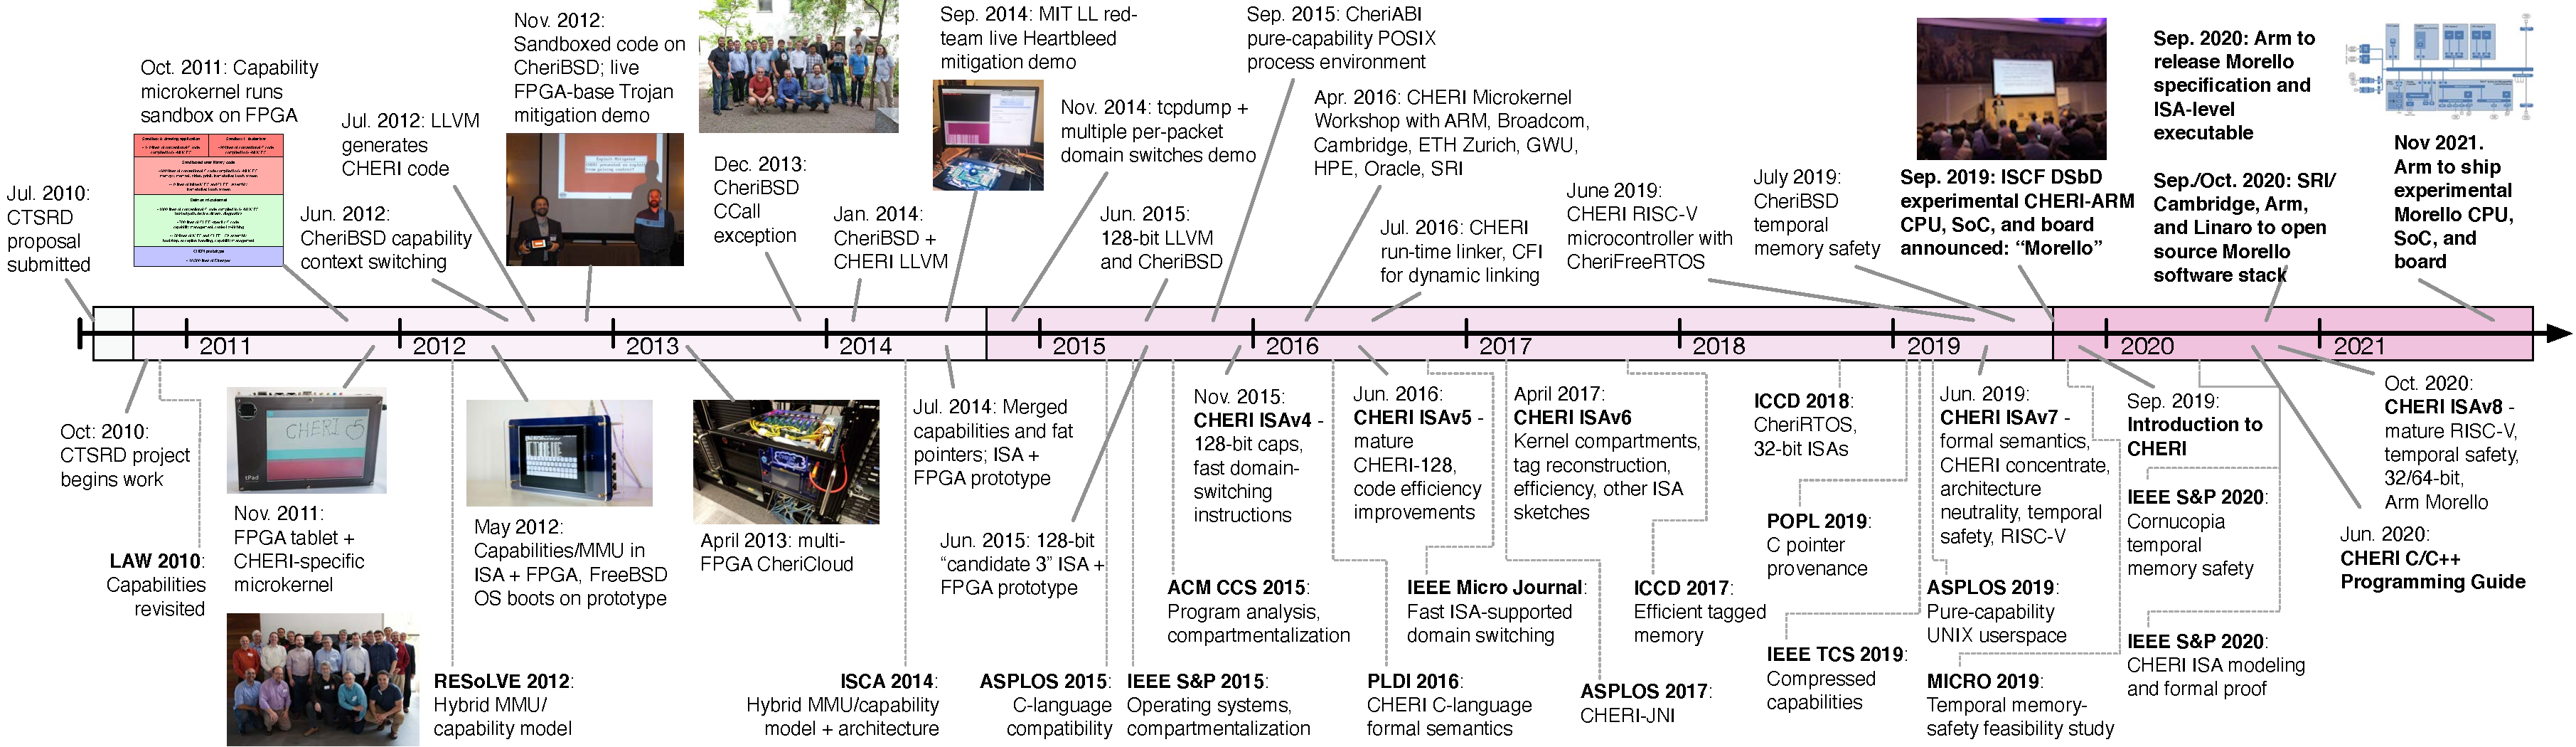
\includegraphics[width=\columnwidth]{20200816-cheri-timeline.pdf}
\caption{CHERI research and development timeline, 2010--2021}
\label{fig:cheri-r-and-d}
\end{center}
\end{sidewaysfigure}

\medskip
\noindent
\textbf{2010--2015: Composing the MMU with a capability-system model}

\nopagebreak
\smallskip
\noindent
A key early design choice was that the capability-system model would be
largely orthogonal to the current MMU-based virtual-memory model, yet also
compose with it cleanly~\cite{woodruff:cheriisca2014}.
We chose to place the capability-system model ``before'' the MMU, causing
capabilities to be interpreted with respect to the virtual, rather than
physical, address space.
This reflected the goal of providing fine-grained memory protection and
compartmentalization within address spaces -- i.e., with respect to the
application-programmer model of memory.

Capabilities therefore protect and implement virtual addresses dereferenced in
much the same way that integer pointers are interpreted in conventional
architectures.
Exceptions allow controlled escape from the capability model by providing
access to privileged capability registers, and execution in privileged rings
grants the ability to manipulate the virtual address space, controlling the
interpretation of virtual addresses embedded in capabilities.

This approach tightly integrates the capability-system model with the pipeline
and register file, requiring that capabilities be first-class primitives
managed by the compiler, held in registers, and so on.
In order to protect capabilities in the virtual address space, we chose to
physically tag them, distinguishing strongly protected pointers from ordinary
data, in turn extending the implementation of physical memory, but also making
that protection entirely independent from (and non-bypassable by) the MMU
mechanism.

\medskip
\noindent
\textbf{2012--2014: Composing C pointers with the capability-system mode}

\smallskip
\noindent
Another key early design choice was the goal of using capabilities to
implement C-language pointers -- initially discretionarily (i.e., as annotated
in the language), and later ubiquitously (i.e., for all virtual addresses in a 
more-secure program).
This required an inevitable negotiation between C-language semantics and the
capability-system model, in order to ensure strong compatibility with current
software~\cite{ChisnallCPDP11,Cerberus-PLDI16}.

For example, C embeds a strong notion that pointers point within buffers.
This requires that CHERI capabilities distinguish the notion of current virtual
address from the bounds of the containing buffer -- while also still providing
strong integrity protection to the virtual address.
This led us to compose
fat-pointer~\cite{trevor:cyclone,Nagarakatte:2009:SHC:1542476.1542504,Necula:2002:CTR:503272.503286} and capability
semantics as the capability-system model evolved.

Similarly, we wished to allow all pointers to be represented as capabilities
-- including those embedded within other data structures -- leading naturally
to a choice to mandatorily tag pointers in memory.
A less obvious implication of this approach is that operations such as memory
copying must be capability-oblivious, maintaining the tag across
pointer-propagating memory operations, requiring that data and capabilities
not only be intermingled in memory, but also in register representation.
Capability registers are therefore also tagged, allowing them to hold data or
capabilities, preserving provenance transparently.

As part of this work, we also assisted with the development of new formal
semantics for the C programming language, ensuring that we met the practical
requirements of C programs, but also assisting in formalizing the protection
properties we offer (e.g., strong protection of provenance validity grounded
in an implied pointer provenance model in C).

CHERI should be viewed as providing primitives to support strong C-language
pointer protection, rather than as directly implementing that protection: it
is the responsibility of the compiler (and also operating system and
runtime) to employ capabilities to enforce protections where desired --
whether by specific memory type, based on language annotations, or more
universally.
The compiler can also perform analyses to trade off source-code and binary
compatibility, enforcing protection opportunistically in responding to various
potential policies on tolerance to disruption.

\medskip
\noindent
\textbf{2014--2015: Fine-grained compartmentalization}

\smallskip
\noindent
A key goal of our approach was to differentiate virtualization (requiring
table-based lookups, and already implemented by the MMU) from protection
(now implemented as a constant-time extension to the pointer primitive), which
would avoid table-oriented overheads being imposed on protection.
This applies to C-language protection, but also to the implementation of
higher-level security constructs such as
compartmentalization~\cite{watson15:cheri,watson2016:microjournal}.

Compartmentalization depends on two underlying elements: strong isolation and
controlled communication bridging that isolation.
Underlying monotonicity in capabilities -- i.e., that a delegated reference
to a set of rights cannot be broadened to include additional rights --
directly supports the construction of confined components within address
spaces.
Using this approach, we can place code in execution with only limited
access to virtual memory, constructing ``sandboxes'' (and other more complex 
structures) within conventional processes.
The CHERI exception model permits transition to a more privileged component
-- e.g., the operating-system kernel or language runtime -- allowing the
second foundation, controlled communication, to be implemented.

Compartmentalization is facilitated by further extensions to the capability
model, including a notion of ``sealed'' (or encapsulated capabilities).
In CHERI, this is implemented as a software-defined capability: one that has
no hardware interpretation (i.e., cannot be dereferenced), and also strong
encapsulation (i.e., whose fields are immutable).
Other aspects of the model include a type mechanism allowing sealed code and
data capabilities to be inextricably linked; pairs of sealed code 
capabilities and data
capabilities can then be used to efficiently describe protection domains via
an object-capability model.
We provide some hardware assistance for protection-domain switching,
providing straightforward parallel implementation of key checks, but leave
the implementation of higher-level aspects of switching to the software
implementation.

Here, as with C-language integration, it is critical that CHERI provide a
general-purpose mechanism rather than enforce a specific policy: the sealed
capability primitive can be used in a broad variety of ways to implement
various compartmentalization models with a range of implied communication
and event models for software.
We have experimented with several such models, including a protection-domain
crossing primitive modeled on a simple (but now strongly protected) function
call, and also on asynchronous message passing.
Our key performance goal was fixed (low) overhead similar to a function call,
avoiding overheads that scale with quantity of memory shared (e.g., as is the
case with table-oriented memory sharing configured using the MMU).

\medskip
\noindent
\textbf{2015--2017: Architectural and microarchitectural efficiency}

\smallskip
\noindent
Side-by-side with development of a mature capability-based architectural
model, we also explored the implications on performance.
This led to iterative refinement of the ISA to improve generated code, but
also substantive efforts to ensure that there was an efficient in-memory
representation of capabilities, as well as microarchitectural implementations
of key instructions.

A key goal was to maintain the principle of a load-store architecture by
avoiding combining computations with memory accesses -- already embodied by
both historic and contemporary RISC architectures.
While pointers are no longer conflated with integer values, a natural
composition of the capability model and ISA maintains that structural goal
without difficulty.

One important effort lay in the reduction from a 256-bit capability (capturing
the requirements of software for 64-bit pointer, 64-bit upper bound, and
64-bit lower bound, as well as additional metadata such as permissions) to a
128-bit compressed representation.
We took substantial inspiration from published work in pointer
compression~\cite{kwon:lowfat}, but found that our C-language compatibility
requirements imposed a quite different underlying model and representation.
For example, it is strictly necessary to support the common C-language idiom
of permitting out-of-bounds pointers (but not dereference), which had been
precluded by many proposed
schemes~\cite{ChisnallCPDP11,Cerberus-PLDI16,davis2019:cheriabi}.
Similarly, the need to support sealed capabilities led to efforts to
characterize the tradeoff between the type space (the number of unique classes
that can be in execution in a CHERI address space) and bounds precision (the
alignment requirements imposed on sealed references).

Another significant effort lay in providing in-memory tags, which are not
directly supported by current DRAM layouts~\cite{joannou2017:tagged-memory, UCAM-CL-TR-936}.
In our initial implementation, we relied on a flat tag table (supported by a
dedicated tag cache).
This imposed a uniform (and quite high) overhead in additional DRAM accesses
across all memory of roughly $10\%$.
We have developed new microarchitectural techniques to improve emulated tag
performance, based on a hierarchical table exploiting sparse use of pointers
in memory, to reduce this overhead to $<2\%$ even with very high pointer
density (e.g., in language runtimes).

\medskip
\noindent
\textbf{2016--2017: Kernel Compartmentalization}

\smallskip
\noindent
Our initial design focus was on supporting fine-grained memory protection
within the user virtual address space, and implicitly, also
compartmentalization.
Beyond an initial microkernel brought up to validate early capability model
variants, kernel prototypes through much of our project have eschewed use of
capability-aware code in the kernel due to limitations of the compiler, but
also because of a focus on large userspace TCBs such as compression libraries,
language runtimes, web browsers, and so on, which are key attack surfaces.

We have more recently returned to in-kernel memory protection and
compartmentalization, where the CHERI model in general carries through without
change -- code executing in the kernel is not fundamentally different from
code executing in userspace.
The key exception is a set of management instructions available to the kernel,
able to manipulate the MMU (and hence the interpretation of capabilities), as
well as control features such as interrupt delivery and exception handling.
We are now extending CHERI to allow the capability mechanism to control access
to these features so that code can be compartmentalized within the kernel.
We are also pursuing changes to the exception-based domain-transition
mechanism used in earlier ISA revisions that shift towards a jump-based model,
which will avoid exception-related overheads in the microarchitecture.

\medskip
\noindent
\textbf{2018--2020: Temporal Memory Safety}

The potential to support strong and deterministic temporal memory safety was
an aim of the CHERI architecture from inception, facilitated by several
architectural features: tagged capabilities allowing accurate identification
of pointers in memory; composition with an MMU to allow invalidation of
portions of the virtual address space; and capability flow control via MMU
and capability permission bits limiting where capabilities could be stored in
memory.
However, we had envisioned this primarily from the perspective of software
compartmentalization, and hence a relatively low overall throughput of
revoked or invalidated capabilities.

With an increased focus on supporting C and C++ memory safety by implementing
all language-level pointers using architectural capabilities, we began to
explore whether heap temporal memory safety could perform adequately using
these techniques.
While for some workloads, they were sufficient, we have expanded the set of
architectural tools to support capability revocation through instructions to
efficiently access tags across regions of memory, and MMU features to allow
tracking of versioned capabilities permitting implementation of load-side
barrier techniques similar to those found in garbage collection appearing in
CHERI ISAv8.
This remains an area of active ongoing research.

\medskip
\noindent
\textbf{2014--2020: Architectural Neutrality}

In our earlier research, CHERI was in all senses an extension to the 64-bit
MIPS ISA.
We took a ``ground up'' view on developing the model, prototyping in a tight
hardware-software co-design loop around the architecture, microarchitecture,
and software, as we brought together ideas about capability-system design and
the baseline ISA.
However, it became apparent that the evolving CHERI protection model in
software related to ideas entirely portable across ISAs: C pointer
implementation, fine-grained memory protection, and software encapsulation.

In 2014, we began a long-running and still ongoing collaboration with Arm
Limited to explore generalizing the model across ISAs, and specifically to
integrate it into the 64-bit ARMv8-A architecture.
This led to the development of a portable architectural model: concept such as
tagged capabilities are essential to CHERI, but not specific to MIPS, ARMv8-A,
or other architectures.
In 2017, in CHERI ISAv6, we sketched integrations of CHERI with the commercial
x86-64 ISA and developing open-source RISC-V ISA.
In CHERI ISAv7, we fully elaborated CHERI-RISC-V, and in CHERI ISAv8 we
polished many aspects of this design based on the experience of implementing a
full hardware-software stack, including three microarchitectures.
In 2019, Arm announced Morello~\cite{arm-morello}, both the integration of
CHERI into ARMv8-A, and also an experimental board implementing the ISA in a
high-end contemporary superscalar processor design.

\section{A Hybrid Capability-System Architecture}

Unlike past research into capability systems, CHERI allows traditional address-space separation, implemented using a memory management unit (MMU), to
coexist with granular decomposition of software within each address space.
Similarly, we have aimed to model CHERI capability behavior not only on strong
capability semantics (e.g., monotonicity), but also to be compatible with
C-language pointer semantics.
As a result, fine-grained memory protection and compartmentalization can be applied selectively throughout existing software
stacks to provide an incremental software migration path.
We envision early deployment of CHERI extensions in selected components of the
TCB's software stack: separation kernels, operating system kernels, programming
language runtimes, sensitive libraries such as those involved in data compression or encryption, and network applications such as web browsers and web
servers.

CHERI addresses current limitations on memory protection and compartmentalization by extending virtual
memory-based separation with hardware-enforced, fine-grained protection within address spaces.
Granular memory protection mitigates a broad range of previously exploitable bugs by coercing common memory-related failures into exceptions that can be handled by the application or operating system, rather than yielding control to the attacker.
The CHERI approach also restores a single address-space programming model for
compartmentalized (sandboxed) software, facilitating efficient, programmable, and robust
separation through the capability model.

We have selected this specific composition of traditional virtual memory with an
in-address-space security model to facilitate technology transition: in CHERI,
existing C-based software can continue to run within processes, and even
integrate with capability-enhanced software within a single process, to provide
improved robustness for selected software components -- and perhaps over time, all
software components.
For example, a sensitive library (perhaps used for image processing) might employ
capability features while executing as part of a CHERI-unaware web browser.
Likewise, a CHERI-enabled application can sandbox and instantiate multiple copies of
unmodified libraries, to efficiently and easily gate access to the rest of application
memory of the host execution environment.

\section{A Long-Term Capability-System Vision}

While we have modeled CHERI as a hybrid capability-system architecture, and in
particular described a well-defined and practical composition with MMU-based
designs, CHERI can also support more ``pure'' capability-oriented hardware and
software designs.
At one extreme in this spectrum, we have begun early experimentation with an
MMU-free processor design offering solely CHERI-based protection for software
use.
We are able to layer a CHERI-specific microkernel over this design, which
executes all programs within a single address-space object-capability model.
This approach might be appropriate to microcontroller-scale systems, to avoid
the cost of an MMU, and in which conventional operating systems might be
inappropriate.
The approach might also be appropriate to very large-scale systems, in which
an MMU is unable to provide granular protection and isolation due to TLB
pressure requiring a shift to very large page sizes.

However, in retaining our primary focus on a hybridization between MMU- and
capability-based approaches, software designs can live at a variety of points
in a spectrum between pure MMU-based and solely CHERI-based models.
A CHERI-based microkernel might be used, for example, within a conventional
operating-system kernel to compartmentalize the kernel -- while retaining an
MMU-based process model.
A CHERI-based microkernel might similarly be used within an MMU-based process
to compartmentalize a large application.
Finally, the CHERI-based microkernel might be used to host solely CHERI-based
software, much as in an MMU-less processor design, leaving the MMU dormant,
or restricted to specific uses such as full-system virtualization -- a task
for which the MMU is particularly well suited.

\section{Threat Model}

%\pgnnote{Model, singular?  Might we have multiple models?  For example,
%    embedded microprocessors might have a different threat model than
%    general-purpose hardware for mobile devices.}
%
%\rwnote{I think I'd take the view that they are the same threat model, as we
%    are concerned with threats originating in locally executing software,
%    whether due to external manipulation (e.g., via network data) or simple
%    local malice.  I'm not sure I perceive a large structural difference for
%    the embedded case -- we are not concerned with physical attacks, etc,
%    where different packaging might affect the story?

CHERI protections constrain code ``in execution'' and allow fine-grained management
of privilege within a framework for controlled separation and communication.
Code in execution can represent the focus of many potentially malicious parties:
subversion of legitimate code in violation of security policies, injection of malicious
code via back doors, Trojan horses, and malware, and also 
denial-of-service attacks.
CHERI's fine-grained memory protection mitigates 
many common attack techniques by implementing bounds and permission checks,
reducing opportunities for the conflation of code and data, corruption of
control flow, and also catches many common exploitable programmer bugs;
compartmentalization constrains successful attacks via pervasive observance of
the principle of least privilege.

Physical attacks on CHERI-based systems are explicitly excluded from our threat model,
although CHERI CPUs might easily be used in the context of tamper-evident or
tamper-resistant systems.
Similarly, no special steps have been taken in our design to counter undesired
leakage of electromagnetic emanations and certain other side channels such as acoustic inferences: 
we take for granted the presence of an
electronic foundation on which CHERI can run.
CHERI will provide a supportive framework for a broad variety of security-sensitive
activities; while not itself a distributed system, CHERI could form a sound foundation for various forms of distributed trustworthiness.

CHERI is an ISA-level protection model that does not address increasingly
important CPU- or bus-level covert and side-channel attacks, relying on the
micro-architecture to limit implicit data flows.
In some sense, CHERI in fact increases exposure: the greater the offers of
protection within a system, the greater the potential impact of unauthorized
communication channels.
As such, we hope side-channel attacks are a topic that we will be able to
explore in future work.  
Overall, we believe that our threat model is realistic and will
lead to systems that can be substantially more trustworthy than
today's commodity systems -- while recognizing that ISA-level protections must
be used in concert with other protections suitable to different threat models.

\section{Formal Methodology}

Throughout this project, we apply formal semantics and reasoning techniques to help avoid
system vulnerabilities.
We are (judiciously) applying formal methodology in
five areas:

\begin{enumerate}
\item Early in the project, we developed a formal semantics for the CHERI-MIPS ISA described in
  SRI's Prototype Verification System (PVS) -- an automated theorem-proving
  and model-checking toolchain -- which can be used to verify the
  expressibility of the ISA, but also to prove properties of critical code.
  For example, we are interested in proving the correctness of software-based
  address-space management and domain transitions.
  We are likewise able to automatically generate ISA-level test suites from
  formal descriptions of instructions, which are applied directly to our
  hardware implementation.

\item We developed extensions to the BSV compiler to export
  an HDL description to SRI's PVS and SAL model checker.
  We also developed a new tool (Smten)
for efficient SMT (Satisfiability Modulo Theories) modeling of designs
 (using SRI's Yices), and another tool for
  automated extraction of key properties from larger designs in the
  BSV language, both
  of which greatly simplify formal analysis.
%PS
%   These tools will allow us to verify low-level properties of the hardware design
%   and use the power of model checking and satisfiability solvers to analyze
%   related properties.
% Ideally they will also help link ISA-level specifications with the CPU implementation. 


\item We then developed more complete CHERI-MIPS ISA models,
  incorporating both
  MIPS and CHERI instructions, first using the L3 and then the Sail instruction-set description
  languages (both of which support automatic generation of executable
  emulators from formal definitions).
  We have used these as the ``golden model'' of instruction
  behavior, against which our test suite is validated, software implementations can
  be tested in order to generate traces of correct processor execution, and so
  on.
  We have used the L3 and Sail models to identify a number of bugs in multiple hardware
  implementations of CHERI-MIPS, as well as to discover software dependences
  on undefined instruction-set behavior.

\item We have used these L3 and Sail models also as a basis for
  mechanised proof of key architectural security properties.
% PS: this is pasted from new intro text
L3 and Sail support automatic generation of versions of the models in
the definition languages of (variously) the
HOL4, Isabelle, and Coq theorem provers. 
Key architectural verification goals including proving not just low-level
properties, such as the monotonicity of each individual instruction
and properties of the CHERI capability compression schemes, but also
higher-level goals such as compartment monotonicity, in which arbitrary code
sequences isolated within a compartment are unable to construct additional
rights beyond those reachable either directly via the register file or
indirectly via loadable capabilities.
We have proven a number of such properties about the CHERI-MIPS ISA, to be
documented in future papers and reports.

% this is now subsumed by the previous bullet
%\item We have proven a number of properties about our ``compressed'' 128-bit
%  capability implementation to ensure that the protection and security
%  properties present in the 256-bit reference semantics (e.g., capability
%  monotonicity) hold of the compressed version -- and that the compression
%  and decompression algorithms are correct.

\item From Sail, we also automatically generate SMT problems, which we
  have used to check properties of our capability compression
  schemes. 


\item We have explored how CHERI impacts a formal specification of C-language
  semantics, improving a number of aspects of our C-language compatibility
  (e.g., as relates to conformant handling of the \ccode{intptr_t} type).
\end{enumerate}

\psnote{Taken out the following, as that draft isn't available (as far
  as I can see).  Presumably it described the earlier PVS work -- do
  we need a pointer to something that does describe that?
``A detailed description of formal methods efforts relating to CHERI may
be found in the emerging draft {\em CHERI Formal Methods
Report}~\cite{CHERI-FM15}.''
}

\section{Protection Model and Architecture}

As our work on CHERI has proceeded, we have transitioned from a view in which
CHERI is an ISA extension to 64-bit MIPS to one in which CHERI is a general
protection model that can be expressed through a variety of approaches
and mappings into multiple underlying ISAs.
This report describes a software-facing protection model
(Chapter~\ref{chap:model}) focused on operating systems and compilers,
specific mapping into the 64-bit MIPS ISA for the purposes of experimentation
and evaluation (Chapters~\ref{chap:architecture}, ~\ref{chap:cheri-mips}
and~\ref{chap:isaref-mips}), and architectural sketches for potential integration
into other ISAs (Chapters~\ref{chap:cheri-riscv} on CHERI-RISC-V,
Chapter~\ref{chap:cheri-x86-64} on CHERI-x86-64, and Arm
Morello~\cite{arm-morello}).
However, we have taken a ``ground-up'' approach utilizing hardware-software
co-design to ensure that concrete mapping exist that
satisfies the practical engineering requirements of architecture,
microarchitecture, compiler, operating system, and applications.
At the time CHERI ISAv8 is published, we are in the throes of transitioning
the bulk of our research from CHERI-MIPS to CHERI-RISC-V and Morello, which
have learned substantially from our initial experiences implementing CHERI.

Our selection of RISC as a foundation for the CHERI capability extensions
is motivated by two factors.
First, simple instruction set architectures are easier to reason about, extend, and implement.
Second, RISC architectures (such as ARM and MIPS) are widely used in network embedded
and mobile device systems such as firewalls, routers, smart phones, and tablets -- markets
with the perceived
flexibility to adopt new CPU facilities, and also an immediate and pressing
need for improved security.
CHERI's new security primitives would also be useful in workstation and server environments,
which face similar security challenges.

CHERI-RISC-V and Arm Morello demonstrate that the abstract CHERI protection
model, as well as our architectural approach, applies to a range of RISC
architectures.
The design principles would also apply to other non-RISC ISAs, such as 32-bit and
64-bit Intel and AMD, but require significantly more adaptation work, as well as careful
consideration of the implications of the diverse set of CPU features found in more CISC-like
architectures.

It is not impossible to imagine pure-software implementations of the CHERI
protection model -- not least, because we use these daily in our work through
both cycle-accurate processor simulations, and a higher-performance but less
microarchitecturally realistic Qemu implementation.
Further, compiler-oriented approaches employing a blend of static checking and
dynamic enforcement could also approximate or implement CHERI protection
semantics (e.g., along the lines of software fault isolation
techniques~\cite{wahbe:sfi} or Google Native Client (NaCl)~\cite{yee:nacl}).
We do, however, hypothesize that these implementations would be difficult to
accomplish without hardware assistance: for example, continuous checking of
program-counter and default data capability bounds, as well as atomic clearing
of tags for in-memory pointers during arbitrary memory writes might come at
substantial expense in software, yet being ``free'' in supporting hardware.

\section{Hardware and Software Prototypes}

As a central part of this research, we have developed reference prototypes of
the CHERI ISA via several CHERI processor designs.
These prototypes allow us to explore,
validate, evaluate, and demonstrate the CHERI approach through realistic
hardware properties and real-world software stacks.
A detailed description of the current prototypes, both from architectural and
practical use perspectives, may be found in our companion papers and technical
reports, described in Section~\ref{sec:publications}.

In our CHERI-MIPS work, we developed two pipelined processor variations that
incorporated our evolving CHERI-MIPS ISA.
These prototypes allowed us to explore ISA design tradeoffs with moderate
microarchitectural realism.
We implement our prototypes in Bluespec SystemVerilog
(BSV)~\cite{Bluespec:TFRG}, allowing us to create highly parameterizable
designs, as well as perform rapid design-space exploration.
Wherever possible, we open source our designs to allow reproduction and reuse
by other researchers.

In addition to our BSV implementations, we have also implemented executable
models using first the L3 ISA modeling language~\cite{Fox2015}, and later
SAIL~\cite{sail-popl2019}.
The SAIL descriptions of CHERI-MIPS and CHERI-RISC-V are used for formal
proof, SMT checking, and also directly incorporated into our CHERI ISA
specification.
We also use an adaptation of the QEMU fast ISA accelerator.

As the CHERI security model is necessarily a hardware-software model, we have
also performed substantial experimentation with software stacks targeting all
of our ISA instantiations of CHERI.
We have an adaptation of the open-source Clang/LLVM compiler suite, LLD
linker, and GDB debugger, which are able to generate code using CHERI
capabilities.
We have adaptations of the FreeRTOS and FreeBSD operating systems to CHERI,
known as CheriFreeRTOS and CheriBSD.
CheriBSD is portable across all of our CHERI-extended architectures:
CHERI-MIPS, CHERI-RISC-V, and Morello.
We use CheriFreeRTOS and CheriBSD on our ISA simulations and also on FGPA.

Throughout, we consider metrics such as microarchitectural disruption, Power
Area and Performance (PPA) on FPGA, dynamic benchmark performance, software
language and source-code disruption, and security as part of our evaluation
cycle.

\chapter{Historical Context and Related Work}
\label{chap:historical}

\nwfnote{There's a great deal more to say here.  Suggestions include
Cambridge's CAP (esp. S-CAP), MIT's M-Machine, Intel iAPX 432, Rekursiv, IBM
System/38, Plessey System 250, RSRE Malvern Flex machine.  Possibly CMU's C.mmp
(and Hydra), and Multics' descriptors as well.}

% Intro prose <<<

As with many aspects of contemporary computer and operating-system design,
many of the origins
of operating-system security can be found at the world's leading research
universities --
especially the Massachusetts Institute of Technology (MIT), the University of Cambridge,
and Carnegie Mellon University.
MIT's Project MAC, which began with MIT's Compatible Time
Sharing System (CTSS)~\cite{corbato:timesharing},
and continued over the next decade with MIT's Multics
project (joint with Honeywell, and originally Bell Labs),
described many central tenets of computer security~\cite{corbato:multics,Graham68}.
Dennis and Van Horn's 1965 {\em Programming Semantics for Multiprogrammed
Computations}~\cite{dennis:semantics} laid out principled hardware
and software approaches
to concurrency, object naming, and security for multi-programmed computer systems --
or, as they are known today, multi-tasking and multi-user computer systems.
Multics implemented a coherent, unified architecture for processes, virtual memory, and protection,
integrating new ideas such as {\em capabilities}, unforgeable tokens of authority, and
{\em principals}, the end users with whom authentication takes place and to whom resources
are accounted~\cite{Saltzer74}.

In 1975, Saltzer and Schroeder surveyed the rapidly expanding vocabulary of computer
security in {\em The Protection of Information in Computer Systems}~\cite{SaltzerSchroeder75}.
They enumerated design principles such as the {\em principle of least privilege}
(which demands that computations run with only the privileges they require) and
the core security goals of
protecting {\em confidentiality}, {\em integrity}, and {\em availability}.
The tension between fault tolerance and security (a recurring debate in
systems literature) saw its initial analysis in Lampson's 1974
{\em Redundancy and Robustness in Memory Protection}~\cite{LampsonRedund}, which
considered ways in which hardware memory protection addressed accidental and
intentional types of failure: e.g., if it is not reliable, it will not be secure,
and if it is not secure, it will not be reliable!  Intriguingly, recent work
by Nancy Leveson and William Young has unified security and human safety
as overarching emergent system properties~\cite{LevesonYoung14}, and allows
the threat model to fall out of the top-down analysis, rather than driving
it.  This work in some sense
unifies a long thread of work that considers trustworthiness as a property 
encompassing security, integrity, reliability, survivability, human safety, 
and so on (e.g.,~\cite{Neumann06holistic,PSOS}, among others).

The Security Research community also blossomed outside of MIT:
Wulf's HYDRA operating system at Carnegie Mellon University (CMU)~\cite{wulf:hydra,CohenJefferson75},
Needham and Wilkes' CAP Computer at
Cambridge~\cite{WilkesNeedham79}, SRI's Provably Secure Operating
System (PSOS)~\cite{PSOSreport,PSOS} hardware-software co-design that included
strongly typed object capabilities,
Rushby's security kernels supported by formal
methods at Newcastle~\cite{Rushby81}, and Lampson's work on
formal models of security
protection at the Berkeley Computer
Corporation all explored the structure of operating-system access control, and
especially the application of capabilities to the protection
problem~\cite{lampson:dynamicprotection,lampson:protection}.
Another critical offshoot from the Multics project was Ritchie and Thompson's UNIX
operating system at Bell Labs, which simplified concepts
from Multics, and became the basis for countless directly and indirectly derived
products such as today's Solaris, FreeBSD, Mac OS X, and Linux operating
systems~\cite{ritchie:unix}.

The creation of secure software went hand in hand with analysis of security flaws:
Anderson's 1972 US Air Force {\em Computer Security Technology Planning
Study} not
only defined new security structures, such as the {\em reference monitor}, but
also analyzed potential attack methodologies such as Trojan horses and
inference attacks~\cite{anderson72}.
Karger and Schell's 1974 report on a security analysis of the Multics system
similarly demonstrated a variety of attacks that bypass hardware and OS
protection~\cite{KargerSchell74}.
In 1978, Bisbey and Hollingworth's {\em Protection Analysis: Project final report} at ISI
identified common patterns of security vulnerability in operating
system design, such as race conditions and incorrectly validated arguments at security
boundaries~\cite{Bisbey78}.
Adversarial analysis of system security remains as critical to the success of security
research as principled engineering and formal methods.

Almost fifty years of research have explored these and other
concepts in great detail, bringing new contributions in hardware, software, language
design, and formal methods, as well as networking and cryptography technologies that
transform the context of operating system security.
However, the themes identified in those early years remain topical and highly influential,
structuring current thinking about systems design.

Over the next few sections, we consider three closely related ideas that directly influence
our thinking for CTSRD: capability security, microkernel OS design, and
language-based constraints.
These apparently disparate areas of research are linked by a duality,
observed by Jim Morris
in 1973, between the enforcement of data types and safety goals in programming languages on one hand, 
and the hardware and software protection techniques explored in operating
systems~\cite{morris:protectionprogramming} on the other hand.
Each of these approaches blends a combination of limits defined by static analysis
(perhaps at compile-time), limits on expression on the execution substrate (such as what
programming constructs can even be represented), and dynamically enforced policy that generates
runtime exceptions (often driven by the need for configurable policy and labeling not known
until the moment of access).
Different systems make different uses of these techniques, affecting expressibility,
performance, and assurance.

% >>>
\section{Capability Systems} % <<<

Throughout the 1970s and 1980s, high-assurance systems were expected
to employ a capability-oriented design that would map program
structure and security policy into hardware enforcement; for example,
Lampson's BCC design exploited this linkage to approximate least
privilege~\cite{lampson:dynamicprotection,lampson:protection}.

Systems such as the CAP Computer at Cambridge~\cite{WilkesNeedham79} and

Ackerman's DEC PDP-1 architecture at MIT~\cite{ackerman:multiprocessing}
attempted to realize this vision through embedding notions of capabilities in
the memory management unit of the CPU, an approach described by Dennis and Van
Horn~\cite{dennis:semantics}.  Levy provides a detailed exploration of segment-
and capability-oriented computer system design through the mid-1980s in {\em
Capability-Based Computer Systems}~\cite{levy:capabilities}.

\subsection{Objects of Authorization}

Dennis and Van Horn's seminal text on capability
systems~\cite{dennis:semantics} defines a capability as a structure that
locates by means of [a unique code or effective name] some computing object,
and indicates the actions that the computation may perform with respect to that
object.'' One may then ask what exactly constitutes a ``computing object,''
and one should not be surprised to learn that there have been several answers
to that question.

\paragraph{Memory Capability Systems}

One answer, and perhaps the simplest, identifies a ``computing object'' with a
mere span of memory.  Such systems closely resemble traditional segmented memory
architectures.

% In their simplest form, there is no direct support for encapsulation
% of private state

\paragraph{Software Object Capability Systems}

In so-called ``object capability'' (``ocap'') systems, ``computing objects''
are identified with pairs of code and private data, as in ``object-oriented
programming.''  These systems may treat objects as entirely opaque, exposing
only one or a series of ``entry'' capabilities, corresponding to object
methods, or may, additionally, optionally offer more direct access to object
data.

Perhaps the most common object capability systems are those built
\emph{without} dedicated hardware support.  Therein, existing abstractions,
such as a privileged supervisory program, are repurposed to provide the
capability substrate.

Entry capability invocation ranges from fully synchronous, in which threads of
control more or less directly transition from within one object to another,
gaining and losing rights as required, to fully asynchronous, in which all
invocations are done my means of message passing between other threads.  In
practice, systems tend to support both options, though they may take one or the
other as their sole ``primitive'' operation.

Ackerman's architecture~\cite{ackerman:multiprocessing} seems to have been
the first to realize the importance of allowing subsystems to construct
multiple, differentiated entry capabilities, to correspond to different
permitted requests (e.g., invoking different methods on different logical
targets within the same subsystem).  A six-bit field, the ``transmitted
word,'' was provided within the entry capability, immune from influence of
the bearer but made available to the subsystem itself on entry.  Similar
facilities have been found in almost all subsequent object capability
systems.%
%
\footnote{CHERI lacks such a field within its capabilities; however, the
\insnref{CInvoke} mechanism can be used to similar effect (recall
Section~\ref{sec:model-sealed-capability-invocation}).}

\paragraph{Hardware Object Capability Systems}

Some systems, including the ill-fated Intel iAPX 432 lineage (including
the BiiN family of systems and the Intel i960MX), have attempted to move
core aspects of the software object capability model into hardware.  Exactly
which features and object types are manifest in hardware depends on the
particular system, but generally one should expect to see a rich notion of
``context'' or ``domain'' of execution and primitives for secure transition
from one to another.

% \paragraph{Hybrid Schemes} iAPX 432 / BiiN. CHERI.

% \subsection{Interpretation of Capabilities}

% >>>
\section{Bounds Checking and Fat Pointers} % <<<

In contrast to prior capability systems, a key design goal for CHERI was to support mapping C-language pointers into capabilities.
In earlier prototypes, we did this solely through base and bounds fields within capabilities, which worked well but required substantial changes to existing C software that often contained programming idioms that violated monotonic rights decrease for pointers.
In later versions of the ISA, we adopt ideas from the C fat-pointer literature, which differentiate the idea of a delegated region from a current pointer: while the base and bounds are subject to guarded manipulation rules, we allow the offset to float within and beyond the delegated region.
Only on dereference are protections enforced, allowing a variety of imaginative pointer operations to be supported.
Many of these ideas originate with the type-safe C dialect Cyclone~\cite{trevor:cyclone}, and see increasing adaptation to off-the-shelf C programs with work such as Softbound~\cite{Nagarakatte:2009:SHC:1542476.1542504}, Hardbound~\cite{Devietti:2008:HAS:1353536.1346295}, and CCured~\cite{Necula:2002:CTR:503272.503286}.
This flexibility permits a much broader range of common C idiom to be mapped into the capability-based memory-protection model.

% >>>
\section{Realizing Capability Systems} % <<<

When a capability systems is encoded, as software or in hardware or with a
mixture of the two, several decisions must be made about how the abstract
objects and actions are to be made manifest.  We highlight two of the major
decisions which must be made.

\subsection{Memory Layout} % <<<

A reified capability system must have some mechanism to distinguish
capabilities from non-capability data or, equivalently, for determining the
semantic type assigned to bits being accessed by the instruction stream.
Broadly speaking, two approaches have emerged: making the type distinction
\emph{intrinsically associated} with the bits in question or associating the
type with the \emph{access path} taken to those bits.

Systems choosing the former option are generally said to be ``tagged
architectures'' or to have ``tagged memory:'' at least one bit is associated
with a granule of memory no larger than a capability, which indicates
whether the associated granule contains capability-typed bits or data-typed
bits.  CHERI is such a design, with one bit per capability-sized and
suitably-aligned piece of memory.  The IBM System/38 uses four bits per
capability-sized piece of memory and requires that they all be set when
attempting to decode a suitably-aligned bit pattern as a capability.

The second variety of systems seem to lack a similarly punchy moniker, but we
may, at the risk of further overloading an already burdened term, call them
``segmented architectures.''  In these systems, it is usually the
(memory-referencing) capabilities themselves that describe the type of the bits
to be found therein; integrity of the capability representations is ensured by
software's careful avoidance of overlapping capabilities.  In simplest
manifestation, a capability to memory designates, in addition to bounds and
permissions, the type of all bits found therein.  Such capabilities are often
described with terms such as ``C-type'' or ``D-type'' (as in the Cambridge CAP
family~\cite{WilkesNeedham79}), emphasising the homogeneous nature of the
segment of memory referenced.  Some other segmented architectures (notably
including the HYDRA microkernel~\cite{CohenJefferson75,Wulf81}) have bifurcated
segments, wherein each contiguous memory segment is effectively two: one
containing capabilities and one containing data; in these systems, capabilities
typically point at the boundary between the two regions and specify length of
each.  Naturally, such segments could carry exclusively capabilities or
exclusively data.

One occasionally sees designs that straddle the distinction between segmented
and tagged architectures.  Therein, capabilities may authorize access to both
data and other capabilities, but there is no requirement that data and
capabilities be separated and contiguous within the authorized memory segment.
For example, in the Coyotos microkernel~\cite{shapiro:2004}, capabilities are
stored in pages of memory accessible only to the capability kernel, but these
``cap pages'' are freely miscible with data pages (either accessible by the
user program or solely by the kernel).  This compromise allows Coyotos to run
on commodity hardware and without a specialized language runtime, but requires
indirection to capabilities in memory: data structures contain pointers to
addresses that will fault if dereferenced in the user program, but these
pointers may be passed to the capability kernel during system calls.

% >>>
\subsection{Indirection of Reference to Capabilities} % <<<

Capability systems also differ in how they name and manipulate capabilities.
In a traditional von Neumann architecture, the primitive indirection mechanism
is the interpretation of an integer as an index into memory.  Virtualization of
this architecture is most often accomplished by inserting a mapping function
from integer ``virtual addresses'' to integer ``physical addresses'' before the
latter are given to the hardware's memory subsystem.  Dennis and Van Horn built
upon this primitive in their initial design of capability
systems~\cite{dennis:semantics}, and so many implementations of capability
systems refer to capabilities by \emph{integers}: the capabilities available to
the current process are, at least logically, enumerated in a translation table
(the ``C-list'' of the process) and the process uses integers to index into
this table.  Data fetch operations through capabilities in such systems specify
the integer \emph{index} (within this table) of the authorizing capability and
the integer \emph{offset} within that capability of the data desired, and the
result is placed into an (integer) register.  Capability fetch, on the other
hand, takes a source index, an offset, and a \emph{target index}: the loaded
capability is placed at the target index within the translation table.  Dually,
while data stores transfer integers from registers to memory, capability stores
transfer a capability from the translation table to memory.

This style of manipulation is especially popular in software capability
systems, as integers abound and a plethora of key-value mapping data structures
are well-understood.  Adding another domain of interpretation to integers is
even something of a time-honored tradition; the manipulation of ``file
descriptors'' may be so habitual to UNIX programmers, for example, that pausing
to reflect that they arise from \emph{design decisions} may be seen as unusual.
Software capability kernels can readily implement this design on behalf of
their (user) programs, even on commodity hardware, by moving all capability
interpretation into the kernel.  As discussed earlier, Coyotos repurposes
virtual addresses (with backing pages beyond the reach of user programs) as
references to capabilities, conflating its capability translation with the
translation structures used for address virtualization.  One often sees small
extensions added in the interest of amortizing the cost of transitions to and
from the supervisor; for example, capability fetch and store operations may be
willing to traverse \emph{paths} (represented by \emph{sequences} of integers),
or multiple capability manipulations may be packaged together, possibly with
other operations, into ``channel programs'' in domain-specific languages
interpreted by the capability kernel.

Even in hardware, such designs are attractive, as they can be ``drop-in
compatible'' with existing MMU-style translation systems, requiring no changes
to the design of the CPU core.  Indeed, the CAP family of
computers~\cite{WilkesNeedham79} divides addresses, as generated by the CPU,
into capability index and offset fields, much as other systems divide (virtual)
addresses into virtual page number and intra-page offset.  In systems where
safe table manipulation operations are directly exposed to the user program,
manipulation of the capability address space can be cheaper than in traditional
MMU-style designs, where the MMU mapping structures are highly guarded and
manipulated solely by the supervisor.
%
\nwfnote{Check, but I think the iAPX432 does as well, yes?}

However, such indirection comes with costs.  While the process as a whole may
satisfy the principle of least authority, the use of integer indices still
presents a challenge to the principle of intensional use.  In the CAP systems,
for example, indexing past the end of a maximally-sized segment, or, indeed,
sufficiently past the end of any segment, will not result in a processor trap,
but will, instead, be interpreted as an access within \emph{a different
capability}.  Even when indices and offsets are maintained separately, there is
nothing, architecturally, that ensures the \emph{provenance} of the index as
such: to confuse a program into acting using an unintended subset of its
authority, it would suffice to corrupt the bits of an integer used as an index.

The use of integer indexes interpreted within a process may also complicate
sharing between processes.  When sending capabilities to another process, the
sender must marshal those capabilities into a (to be) shared segment, as the
indices by which the sender refers to these capabilities are useless to the
recipient.  (The situation is analogous to the passing of integer virtual
addresses in shared memory segments: because the segments may be mapped at
different offsets by participating processes, even if the addresses reference
within the segment in one process, they may be meaningless to another.)

CHERI takes a subtly different approach, in which capabilities are loaded into
CPU registers.  The instruction stream combines in-register capabilities with
offsets to make memory accesses.  As with the systems employing separated index
and offset fields, it is impossible for an out-of-bounds offset to shift the
capability against which the offset is interpreted.  Moreover, CHERI ensures
the architectural validity of the derivation of the capability being used to
authorize the access.%
%
\footnote{That is not to say that it is impossible for a CHERI program to have
bugs or to otherwise give an attacker control over which capability is used in
a given access.  It does, however, rule out a large class of historically
powerful attack vectors in which adversarial data is \emph{directly}
interpreted as an integer address.}

% >>>
% >>>
\section{Capabilities In Hardware} % <<<

\subsection{Tagged-Memory Architectures} % <<<

Perhaps the most well-known tagged machine design these days is that of the
Burroughs Large systems, starting with the B5000, designed in 1961.  Both
contemporaneous \cite{Creech69,Burroughs-B6700,Organick73} and retrospective
\cite{Mayer82,Barton87} material about this family of machines is available
for the curious reader, as is an interesting report of a concerted
penetration test against Burroughs' operating system \cite{Wilkinson}.  For
present purposes, however, we focus on its memory model and, in particular,
its use of tags and descriptors.  In the B5000, each word was equipped with
a bit distinguishing its intended use as either data or instructions.  The
later B6500 moved to a three-bit tag; we may (very) roughly summarize this
latter taxonomy as differentiating between data words, program instructions,
and pointers of various sorts.  In several cases, the tags were used to
convey \emph{type} information to the CPU, so that, for example, the unique
addition instruction would operate on single-precision words or
double-precision word pairs depending on the data tag of its operands
\cite[p. 97]{Organick73}, or the processor's ``step and branch'' instruction
can manipulate a ``step index word'' containing all of the current value,
increment, and limit of iteration \cite[p. 7-5]{Burroughs-B6700}.  More
naturally (to a CHERI-minded reader, at least), loads and stores and
indirect transfers of control required their operands to be properly tagged,
and subroutine entry generates tagged return addresses on the stack
\cite[ch. 7]{Burroughs-B6700}.

While concerned mostly with detection of software bugs, rather than any
consideration of system security, Gumpertz's \emph{Error Detection with
Memory Tags} \cite{Gumpertz81} deserves mention.  The tags in this work are
not used to determine operations (as they might have been in the Burroughs
B5000) but rather as additional checks on tag-independent operations.
Gumpertz's design focuses on light-weight checks, performed in parallel with
CPU operations and makes it ``possible to check an arbitrary number of
assertions using only a small tag of fixed size'' \cite[p.  i]{Gumpertz81},
which is similar to CHERI's imbuing of an arbitrary number of bits (i.e.,
the width of a capability) with architectural semantics using a single,
external tag bit.

% >>>
\subsection{Segmented Architectures} % <<<

\subsubsection{Cambridge CAP Computer} % <<<

The family of Cambridge CAP computer designs%
%
\footnote{The CAP experiment seems to have produced one physical, heavily
microprogrammed CPU design and at least three different microcode programs.}
%
\cite{WilkesNeedham79}
%
are, at their core, capability-based refinements of earlier,
base-and-length memory segmentation schemes.  In these earlier schemes, the
CPU computes offsets within a segment and then dereferences memory as a pair
of an offset and an \emph{index} into a segment table; on dereference, the
offset is checked to be in bounds, and the indirection between segment and
memory---usually just an addition operation---is performed to yield the
``linear'' (or ``physical'') address used to communicate with the memory
subsystem.  Programs running on the CAP computer similarly have a virtual
address space consisting of pairs of indices into a \emph{capability table}
and offsets within those capabilities.  While the exact interpretation and
mechanisms of the capabilities of each CAP design differed, there are
commonalities across the family.

The CAP computers interpreted virtual addresses, held in arithmetic
registers, as pairs of a capability specifier and a 16-bit index to a word
within that capability.  On the CAP computers, capabilities are interpreted
only after a virtual address has been dispatched from the CPU.  This
separation of construction and interpretation violates our principle of
intensional use and enables certain kinds of confusion.  To wit, overflowing
the offset results in a potentially in-bound offset \emph{within a different
capability}.  This is in stark contrast to a pure-capability CHERI design,
wherein capabilities \emph{supplant} virtual addresses and are directly
manipulated while in registers, making it impossible for operations on a
capability's offset to change to \emph{which} capability the offset is
relative.%
%
\footnote{Though CHERI does have its IDC mechanism for compatibility with
non-capability programs.  Similar confusion is possible in hybrid
applications if an offset intended to be relative to one capability is
instead used with another, for example, due to improper management of IDC.
Historically, similar confusion can arise in the more common segmentation
models, as seen in, for example, Intel's X86 CPUs, in which segment table
indices (``segment selectors'') are held in dedicated registers and only
combined with offsets (held in arithmetic registers) by the instruction
stream.}

% \subsubsection{CAP-1}

% \subsubsection{CAP-3}

% >>>
% >>>
% >>>
\section{Microkernels} % <<<

Denning has argued that the failures of capability hardware projects were classic failures of
large systems projects, an underestimation of the complexity and cost of reworking an entire system
design, rather than fundamental failures of the capability model~\cite{denning:faulttolerance}.
However, the benefit of hindsight suggests that the earlier demise of hardware capability systems
was a result of three related developments in systems research: microkernel OS design, a
related interest from the security research community in security kernel design, and
Patterson and Sequin's Reduced Instruction-Set Computers (RISC)~\cite{patterson:risc}.

With a transition from complex instruction set computers (CISC) to reduced instruction
set computers (RISC), and a shift away from microcode toward operating system implementation
of complex CPU functionality, the attention of security researchers turned to microkernels.

Carnegie Mellon's HYDRA~\cite{CohenJefferson75,Wulf81} embodied this approach, in which microkernel
message passing between separate tasks stood in for hardware-assisted security domain crossings
at capability invocation.
HYDRA developed a number of ideas, including the relationship between
capabilities and object references, refined the {\em object-capability} paradigm, 
and
further pursued the separation of policy and mechanism.\footnote{Miller has expanded on the
object-capability philosophy in considerable depth in his 2006 PhD dissertation,
{\em Robust composition: towards a unified approach to access control and concurrency
control}~\cite{miller:robustcomposition}}
Jones and Wulf argue through the HYDRA design that the capability model allows the
representation of a broad range of
system policies as a result of integration with the OS object model, which in turn facilitates
interposition as a means of imposing policies on object access~\cite{Jones74}.

Successors to HYDRA at CMU include Accent and Mach~\cite{Accent,accetta:mach},
both microkernel systems intended to
explore the decomposition of a large and decidedly un-robust operating system kernel.
In microkernel designs, traditional OS services, such as the file system, are
migrated out of ring 0 and into user processes, improving debuggability and
independence of failure modes.
They are also based on mapping of capabilities as object references into IPC pipes
({\em ports}), in which messages on ports represent methods on objects.
This shift in operating system design went hand in hand with a related analysis in the
security community: Lampson's model for capability security was, in fact, based on pure
message passing between isolated processes~\cite{lampson:protection}.
This further aligned with proposals by Andrews~\cite{andrews:partitions} and
Rushby~\cite{Rushby81} for a {\em security kernel}, whose responsibility lies
solely in maintaining isolation, rather than the provision of higher-level services such as file
systems.
Unfortunately, the shift to message passing also invalidated Fabry's semantic argument for
capability systems, namely, that by offering a single namespace shared by all protection domains,
the distributed system programming problem could be avoided~\cite{fabry:caseforcapabilities}.

A panel at the 1974 National Computer Conference and Exposition (AFIPS) chaired by Lipner
brought the design goals and choices for microkernels and security kernels clearly into
focus: microkernel developers sought to provide flexible platforms for OS research with an
eye towards protection, while security kernel developers aimed for a high assurance platform
for separation, supported by hardware, software, and formal
methods~\cite{lipner:securitykernels}.

The notion that the microkernel, rather than the hardware, is responsible for implementing
the protection semantics of capabilities also aligned well with the simultaneous research (and
successful technology transfer) of RISC designs, which eschewed microcode by shifting complexity
to the compiler and operating system.
Without microcode, the complex C-list peregrinations of CAP's capability unit, and protection domain
transitions found in other capability-based systems,
become less feasible in hardware.
Virtual memory designs based on fixed-size pages and simple semantics
have since been standardized throughout the industry.

Security kernel designs, which combine a minimal kernel focused entirely on correctly
implementing protection, and rigorous application of formal methods, formed the foundation
for several secure OS projects during the 1970s.
Schiller's security kernel for the PDP-11/45~\cite{Schiller75} and Neumann's Provably
Secure Operating System~\cite{PSOS} design study were ground-up operating system designs
based soundly in formal methodology.\footnote{PSOS's ground-up design included ground-up hardware,
whereas Schiller's design revised only the software stack.}
In contrast, Schroeder's MLS kernel design for Multics~\cite{schroeder:multicssecuritykernel},
the DoD Kernelized Secure Operating System (KSOS)~\cite{McCauley}, and Bruce Walker's UCLA UNIX
Security Kernel ~\cite{walker:uclasecureunix} attempted to slide MLS kernels underneath existing
Multics and UNIX system designs.
Steve Walker's 1980 survey of the state of the art in trusted operating systems provides a summary
of the goals and designs of these high-assurance security kernel
designs~\cite{walker:adventtrusted}.

The advent of CMU's Mach microkernel triggered a wave of new research into security kernels.
TIS's Trusted Mach (TMach) project extended Mach to include mandatory access
control, relying on enforcement in the microkernel and a small number of
security-related servers to implement the TCB to accomplish sufficient
assurance for a TCSEC B3 evaluation~\cite{BranstadLandauer89}.
Secure Computing Corporation (SCC) and the National Security Agency (NSA) adapted PSOS's
type enforcement from LoCK (LOgical Coprocessor Kernel)
for use in a new Distributed
Trusted Mach (DTMach) prototype, which built on the TMach approach while adding
new flexibility~\cite{sebes:dtmach}.
DTMach, adopting ideas from HYDRA, separates mechanism (in the microkernel) from
policy (implemented in a userspace security server) via a new reference monitor
framework, FLASK~\cite{spencer:flask}.
A significant focus of the FLASK work was performance: an access vector cache is
responsible for caching access control decisions throughout
the OS to avoid costly up-calls and message passing (with associated context switches) to the
security server.
NSA and SCC eventually migrated FLASK to the FLUX microkernel developed by the University of
Utah in the search for improved performance.
Invigorated by the rise of
microkernels and their congruence with security kernels, 
this flurry of operating system security research also faced the limitations
(and eventual rejection) of the microkernel approach by the computer industry --
which perceived the performance overheads as too great.

Microkernels and mandatory access control have seen another experimental
composition in the form of Decentralized Information Flow Control (DIFC).
This model, proposed by Myers, allows applications to assign information flow labels
to OS-provided objects, such as communication channels, which are propagated and
enforced by a blend of static analysis and runtime OS enforcement, implementing
policies such as taint tracking~\cite{myers:difc} -- effectively, a composition of mandatory
access control and capabilities in service to application security.
This approach is embodied by Efstathopoulos et al.'s Asbestos~\cite{efstathopoulos:asbestos}
and Zeldovich et al.'s Histar~\cite{zeldovich:histar} research operating systems.

Despite the decline of both hardware-oriented and microkernel
capability system design, capability models continue to interest both
research and industry.  Inspired by the proprietary KeyKOS
system~\cite{hardy:keykos}, Shapiro's EROS~\cite{shapiro:eros} (now
CapROS) and Coyotos~\cite{shapiro:2004} continued the investigation of higher-assurance software
capability designs, and
seL4~\cite{klein:sel4}, a formally verified, capability-oriented
microkernel, has also continued along this avenue.
General-purpose systems also have adopted elements of the microkernel capability design
philosophy, such as Apple's Mac OS X~\cite{apple:macosx}
(which uses Mach interprocess communication (IPC)
objects as capabilities) and 
Cambridge's Capsicum~\cite{Watson10} research project 
(which attempts to blend capability-oriented design with UNIX).

More influentially, Morris's suggestion of capabilities at the programming language
level has seen widespread deployment.
Gosling and Gong's Java security model blends language-level type safety with a capability-based
virtual machine~\cite{gosling:javalanguage,Gong+97}.
Java maps language-level constructs (such as object member and method protections) into
execution constraints enforced by a combination of a pre-execution bytecode verification
and expression constraints in the bytecode itself.
Java has seen extensive deployment in containing potentially (and actually) malicious
code in the web browser environment.
Miller's development of a capability-oriented E language~\cite{miller:robustcomposition},
Wagner's Joe-E capability-safe
subset of Java~\cite{mettler:joee}, and Miller's Caja capability-safe subset of JavaScript continue a
language-level exploration of capability security~\cite{miller:caja}.

% >>>
\section{Language and Runtime Approaches} % <<<

Direct reliance on hardware for enforcement (which is central to both historic 
and current systems) is not the only approach to isolation enforcement.
The notion that limits on expressibility in a programming language can be used to
enforce security properties is frequently deployed in contemporary systems to
supplement coarse and high-overhead operating-system process models.
Two techniques are widely used: virtual-machine instruction sets (or perhaps physical
machine instruction subsets) with limited expressibility, and more expressive languages
or instruction sets combined with type systems and formal verification techniques.

The Berkeley Packet Filter (BPF) is one of the most frequently cited
examples of the virtual machine approach: user processes upload pattern matching programs
to the kernel to avoid data copying and context switching when sniffing network packet
data~\cite{mccanne:bpf}.
These programs are expressed in a limited packet-filtering virtual-machine instruction
set capable of expressing common constructs, such as accumulators, conditional forward
jumps, and comparisons, but are incapable of expressing arbitrary pointer arithmetic that
could allow escape from confinement, or control structures such as loops that might lead
to unbounded execution time.
Similar approaches have been used via the type-safe Modula 3 programming language in
SPIN~\cite{bershad:spin}, and the DTrace instrumentation tool that, like BPF, uses a narrow
virtual instruction set to implement the D language~\cite{cantrill:dtrace}.

Google's Native Client (NaCl) model edges towards a verification-oriented approach, in which
programs must be implemented using a `safe' (and easily verified) subset of the x86 or ARM
instruction sets, which would allow confinement properties to be validated~\cite{yee:nativeclient}.
NaCl is closely related to Software Fault Isolation (SFI)~\cite{wahbe:sfi}, in which safety
properties of machine code are enforced through instrumentation to ensure no unsafe access,
and Proof-Carrying Code (PCC), in which the safe properties of code are demonstrated through
attached and easily verifiable proofs~\cite{necula:pcc}.
As mentioned in the previous section, the 
Java Virtual Machine (JVM) model is similar; 
it combines runtime execution constraints of a
restricted, capability-oriented bytecode with a static verifier run over
Java classes before they can be loaded into the execution environment; this
 ensures that only safe accesses have been expressed.
C subsets, such as Cyclone~\cite{trevor:cyclone}, and type-safe languages such as
Ruby~\cite{ruby}, offer similar safety guarantees, which can be leveraged to provide
security confinement of potentially malicious code without hardware support.

These techniques offer a variety of trade-offs relative to CPU enforcement 
of the process model.  For example, some (BPF, D) limit expressibility that 
may prevent potentially useful constructs from being used, such as loops
bounded by invariants rather than instruction limits; in doing so, 
this can typically impose potentially significant performance overhead. 
Systems such as FreeBSD often support just-in-time compilers (JITs) that 
convert less efficient virtual-machine bytecode into native code subject to 
similar constraints, addressing performance but not expressibility 
concerns~\cite{mckusick:freebsd}.

Systems like PCC that rely on proof techniques have had limited impact in
industry, and often align poorly with widely deployed programming languages (such as C)
that make formal reasoning difficult.
Type-safe languages have gained significant ground over the last decade, with widespread use
of JavaScript and increasing use of functional languages such as OCaML~\cite{remy:ocaml}; they offer
many of the performance benefits with improved expressibility, yet have had little impact on
operating system implementations.
However, an interesting twist on this view is described by Wong in Gazelle, in
which the observation is made that a web browser is effectively an operating system by virtue of
hosting significant applications and enforcing confinement between different
applications~\cite{wang:gazelle}.
Web browsers frequently incorporate many of these techniques including Java Virtual Machines and
a JavaScript interpreter.

% >>>
\section{Influences of Our Own Past Projects} % <<<

Our CHERI capability hardware design responds to all these design trends -- and their problems.
Reliance on traditional paged virtual memory for strong address-space separation, as used in Mach,
EROS, and UNIX, comes at significant cost: attempts to compartmentalize system software and
applications sacrifice the programmability benefits of a language-based capability design (a point made
convincingly by Fabry~\cite{fabry:caseforcapabilities}), and introduce significant performance
overhead to cross-domain security boundaries.
However, running these existing software designs is critical to improve the odds of technology
transfer, and to allow us to incrementally apply ideas in CHERI to large-scale contemporary applications
such as office suites.
CHERI's hybrid approach allows a gradual transition from virtual address separation to capability-based
separation within a single address space, 
thus 
restoring programmability and performance so as to facilitate
fine-grained compartmentalization throughout the system and its applications.

We consider some of our own past system designs in greater detail,
especially as they relate to CTSRD:

\paragraph{Multics} % <<<
The Multics system incorporated many new concepts in hardware, software,
and programming~\cite{Organick,DaleyNeumann}.
The Multics hardware provided independent virtual
memory segments, paging, interprocess and intra-process separation,
and cleanly separated address spaces.
The Multics software provided
symbolically named files that were dynamically linked for efficient
execution, rings of protection providing layers of security and system
integrity, hierarchical directories, and access-control lists.
Input-output was also symbolically named and dynamically linked, with
separation of policy and mechanism, and separation of device
independence and device dependence.
A subsequent redevelopment of the two
inner-most rings enabled Multics to support multilevel security in the
commercial product~\cite{schroeder:multicssecuritykernel}.
Multics was implemented in a stark subset (EPL) of
PL/I that considerably diminished the likelihood of many common
programming errors.
In addition, the stack discipline inherently
avoided buffer overflows.

% >>>
\paragraph{PSOS} % <<<
SRI's Provably Secure Operating System hardware-software design was formally
specified in a single language (SPECIAL), 
with encapsulated modular abstraction, interlayer state mappings,
and abstract programs relating each layer to those on which it
depended~\cite{PSOS,NeumannFeiertag03}.
The hardware design provided tagged, typed, unforgeable
capabilities required for every operation, with identifiers that were unique
for the lifetime of the system.  In addition to a
few primitive types, application-specific object types could be defined and
their properties enforced with the hardware assistance provided by the
capability-based access controls.  The design allowed application layers to
efficiently execute instructions, with object-oriented 
capability-based addressing directly to the hardware -- despite appearing at
a much higher layer of abstraction in the design specifications.

%{\em Newcastle Distributed Secure System}~\cite{Rushby+Randell83c}
%
%{\em Separation Kernels}~\cite{Rushby81,Rushby82,Rushby04:separation}

% >>>
\paragraph{MAC Framework} % <<<
The MAC Framework is an OS reference-monitor framework used in FreeBSD, also
adopted in Mac OS X and iOS, as well as other FreeBSD-descended operating
systems such as Juniper Junos and McAfee Sidewinder~\cite{watson13}.
Developed in the DARPA CHATS program, the MAC Framework allows static and
dynamic extension of the kernel's access-control model, supporting
implementation of {\em security localization} --
that is,  
 %%% IS THIS CORRECT?  IT WAS UNGRAMMATICAL AND AMBIGUOUS
the adaptation of the OS
security to product and deployment-specific requirements.
The MAC Framework (although originally targeted at classical mandatory access
control models) found significant use in application sandboxing, especially in
Junos, Mac OS X, and iOS.
One key lesson from this work is the importance of longer-term thinking about
security-interface design, 
including
interface stability and
support for multiple policy models; these are especially important in
instruction-set design.
Another important lesson is the increasing criticality of extensibility of not
just the access-control model, but also the means by which remote principals
are identified and execute within local systems: 
not only is consideration of classical UNIX users inadequate, 
but also there is a need to allow widely varying policies and
notions of remote users executing local code across systems.
These lessons are taken to heart in capability systems, which carefully
separate policy and enforcement, but also support extensible policy through
executable code.

% >>>
\paragraph{Capsicum} % <<<
Capsicum is a lightweight OS capability and sandbox framework included in
FreeBSD 9.x and later~\cite{Watson10,Watson10a}.
Capsicum extends (rather than replaces) UNIX APIs, and
provides new kernel primitives
(sandboxed capability mode and capabilities) and a userspace sandbox
API.
These tools support compartmentalization of monolithic UNIX applications
into logical applications, an increasingly common goal supported poorly by
discretionary and mandatory access controls.
This approach was demonstrated by adapting core FreeBSD utilities and
Google's Chromium web browser to use Capsicum primitives; it showed
significant simplicity and robustness benefits to Capsicum over other
confinement techniques.
Capsicum provides both inspiration and motivation for CHERI: its hybrid
capability-system model is transposed into the ISA to provide
compatibility with current software designs, and its demand for finer-grained
compartmentalization motivates CHERI's exploration of more scalable
approaches.

% >>>
% >>>
\section{A Fresh Opportunity for Capabilities} % <<<

Despite an extensive research literature exploring the potential of
capability-system approaches, and limited transition to date, we believe
that the current decade has been the time to revisit these
ideas, albeit through the lens of contemporary problems and with insight gained through decades of research into security and systems design.
As described in Chapter~\ref{chap:introduction}, a transformed threat
environment deriving from ubiquitous computing and networking, and the
practical reality of  widespread exploitation of software vulnerabilities, 
both
provide a strong motivation to investigate improved processor foundations for
software security.
This change in environment has coincided with improved 
and more rapid
hardware prototyping
techniques and higher-level hardware-definition languages that facilitate
academic hardware-software system research at larger scales; without them we
would have been unable to explore the CHERI approach in such detail.
Simultaneously, our understanding of operating-system and programming-language
security has been vastly enhanced by several decades of research; 
in particular, recent
development of the hybrid capability-system Capsicum model suggests a strong alignment between
capability-based techniques and successful mitigation approaches that can be
translated into processor design choices.

% >>>

% vim: foldmethod=marker:foldmarker=<<<,>>>

\chapter{Conclusion}
\label{chap:conclusion}
The CHERI project is in its tenth year -- an evolution described in detail in
Chapter~\ref{chap:research}.
Throughout the project, we have utilized hardware-software co-design, with an
increasing focus on also co-designing with formal models.
For the last several years, we have increased our focus on transition,
including through a close collaboration with Arm in the development of their
Morello architecture and hardware prototype~\cite{arm-morello}.
Our contributions include:

\begin{enumerate}
\item We developed the CHERI protection model and reference CHERI-MIPS and
  CHERI-RISC-V Instruction-Set Architectures, which  offer low-overhead
  fine-grained memory protection and support scalable software
  compartmentalization based on a hybrid capability model.
  Over several generations of the ISA, we refined integration with
  conventional
  RISCs ISA, composed the capability-system model with the MMU, pursued strong
  C-language compatibility, developed compartmentalization features based on
  an object-capability model, refined the architecture to improve performance
  and adoptability through features such as compressed 128-bit capabilities,
  introduced support for temporal memory safety,
  and developed the notion of a portable protection model that can be applied
  to further ISAs.
  We also explored the implications of CHERI on 32-bit microcontroller
  architectures
  that do not have MMUs, giving capabilities a physical interpretation, and
  also taking into account common microcontroller microarchitectural choices.

\item Employed increasingly complete formal models of the protection model and
  ISA semantics.
  We began by using PVS/SAL formal models of the ISA to analyze
  expressivity and security.
  Subsequently, and in close collaboration with the University of Cambridge's
  EPSRC-funded Rigorous Engineering of Mainstream Systems (REMS) Project and
  DARPA-funded CHERI Instruction-set Formal Verification (CIFV), we
  developed L3 and SAIL formal models suitable to act as a gold model for
  testing, to use in automated test generation, and as inputs to formal
  verification tools to prove ISA-level security properties.
  We have also used formal modeling to explore how CHERI interacts with
  C-language semantics.
  In the future, we hope to employ these models in support of hardware and
  software verification.

\item Elaborated the ISA feature set in CHERI to support real-world operating
  systems -- primarily this has consisted of developing mature compositions of
  CHERI's concepts with system features such as the MMU and exception model.
  We have also spent considerable time refining successive versions of
  the ISA intended to better support high levels of MMU-based operating-system
  and C-language compatibility, as well as automatic use by compilers.
  This work has incorporated ideas from, but also gone substantially beyond,
  the C-language fat-pointer and software compartmentalization research
  literature.

\item Created our CheriBSD and CheriFreeRTOS operating-system prototypes.
  These reference designs explore how CHERI integration with the OS can
  improve both OS and application security.
  We created prototype memory protection and software compartmentalization
  environments including CheriBSD's CheriABI process environment, and multiple
  approaches to sandboxing.
  We have applied CHERI to protection of key system libraries, but also the
  operating system kernel itself.
  This has included substantial baseline OS infrastructure work, including
  porting FreeBSD to the RISC-V architecture.

\item Prototyped, tested, and refined CHERI ISA extensions across multiple CPU
  architectures.
  We have open sourced reference MIPS and RISC-V processor designs, and the
  QEMU ISA-level emulator, on order to allow reproducible experimentation with
  our approach, as well as to act as an open-source platform for other future
  hardware-software research projects.

\item Adapted the Clang/LLVM compiler suite to be able to generate CHERI ISA
  instructions as directed by C-language annotations, exploring a variety of
  language models, code-generation models, and ABIs.
  We have explored two new C-language models and associated code generation:
  a hybrid in which explicitly annotated or automatically inferred pointers
  are compiled as capabilities; and a pure-capability model in which all
  pointers and implied virtual addresses are compiled as capabilities.
  Similarly, we have begun an exploration of how CHERI affects program
  linkage, with early prototype integration with the compile-time and run-time
  linkers.
  These collectively provide strong spatial and pointer protection for both
  data and code pointers.
  We have upstreamed substantial improvements to Clang/LLVM MIPS support, as
  well as changes making it easier to support ISA features such as extra-wide
  pointers utilized in the CHERI ISA.
  We have also begun to explore how CHERI can support higher-level language
  protection, such as by using it to reinforce memory safety and security for
  native code running under the Java Native Interface (JNI).

\item Began to develop semi-automated techniques to assist software
  developers in compartmentalizing applications using Capsicum and CHERI
  features.
  This is a subproject known as Security-Oriented Analysis of Application
  Programs (SOAAP), and performed in collaboration with Google.

\item Collaborated with Arm on the creation of Morello~\cite{arm-morello}, a
  tight integration of CHERI into the ARMv8-A architecture as well as a
  reference industrial quality microarchitecture.
  Morello boards will ship for experimental use in late 2021 along with our
  complete CHERI software stack.
\end{enumerate}

Collectively, these accomplishments have validated our research hypotheses:
that a hybrid capability-system architecture and viable supporting
microarchitecture can support low-overhead memory protection and fine-grained
software compartmentalization while maintaining strong compatibility with
current RISC, MMU-based, and C/C++-language software stacks, as well as an
incremental software adoption path to additional trustworthiness.
Further, the resulting protection model, co-designed around a specific ISA and
concrete extensions, is in fact a generalizable and portable protection model
that has been applied to other ISAs; it is suitable for a multitude of
implementations in architecture and microarchitecture.
Formal methodology deployed judiciously throughout the design and
implementation process has increased our confidence that the resulting design
can support robust and resilient software designs.

\section{Future Work}
We have made a strong beginning, but clearly there is still much to do in our
remaining CHERI efforts.
Our ongoing key areas of research include:

\begin{itemize}
\item
Continuing to refine performance with respect to both the architecture (e.g.,
models for capability compression) and microarchitecture (e.g., as relates to
efficient implementations of compression and tagged memory).

\item
Exploring how CHERI's features might be scaled up (e.g., to superscalar
processor designs), down (e.g., to 32-bit microcontrollers without MMUs), and
to other compute types (e.g., DMA engines, GPUs, and so on).
Also, looking at how CHERI interacts with other emerging hardware technologies
such as non-volatile memory, where CHERI may support more rapid, robust, and
secure adoption.

\item
Continuing to elaborate how CHERI should affect the design of operating
systems (whether hybrid systems such as CheriBSD, or clean-slate designs),
languages (e.g., C, C++, Java, and so on), and runtimes (e.g., system
libraries, run-time linking, and higher-level language runtimes).

\item
Continuing to explore how CHERI affects software tracing and debugging; for
example, through capability-aware software debuggers.

\item
Continuing to explore potential models for software compartmentalization, such
as clean-slate microkernel-style message passing grounded in CHERI's
object-capability features, but not hybridized with conventional OS designs.
In addition, continuing to investigate potential approaches to semi- or
fully automated software compartmentalization.

\item
Continuing our efforts to develop and utilize formal models of the
microarchitecture, architecture, operating system, linkage model, language
properties, compilation, and higher-level applications.
This will help us understand (and ensure) the protection benefits of CHERI up
and down the hardware-software stack.
\end{itemize}


\appendix

\chapter{CHERI ISA Version History}
\label{app:versions}

This appendix contains both a high-level summary of prior CHERI ISA versions
(Section~\ref{sec:detailed-cheri-isa-version-change-history}),
and also a detailed change log for each version
(Section~\ref{sec:detailed-cheri-isa-version-change-history}).
This report was previously made available as the {\em CHERI Architecture
Document}, but is now the {\em CHERI Instruction-Set Architecture}.

\section{CHERI ISA Specification Version Summary}
\label{sec:cheri-isa-specification-version-summary}

A short summary of key ISA versions is presented here:

\begin{description}
\item[CHERI ISAv1 - 1.0--1.4 - 2010--2012]
  Early versions of the CHERI ISA explored the integration of capability
  registers and tagged memory -- first in isolation from, and later in
  composition with, MMU-based virtual memory.
  CHERI-MIPS instructions were targeted only by an extended assembler, with an
  initial microkernel (``Deimos'') able to create compartments on bare metal,
  isolating small programs from one another.
  Key early design choices included:
  \begin{itemize}
  \item to compose with the virtual-memory mechanism by being an
    in-address-space protection feature, supporting complete MMU-based OSes,
  \item to use capabilities to implement code and data pointers for C-language
    TCBs, providing reference-oriented, fine-grained memory protection and
    control-flow integrity,
  \item to impose capability-oriented monotonic non-increase on pointers to
    prevent privilege escalation,
  \item to target capabilities with the compiler using explicit capability
    instructions (including load, store, and jumping/branching),
  \item to derive bounds on capabilities from existing code and data-structure
    properties, OS policy, and the heap and stack allocators,
  \item to have both in-register and in-memory capability storage,
  \item to use a separate capability register file (to be consistent with the
    MIPS coprocessor extension model),
  \item to employ tagged memory to preserve capability integrity and
    provenance outside of capability registers,
  \item to enforce monotonicity through constrained manipulation instructions,
  \item to provide software-defined (sealed) capabilities including a
    ``sealed'' bit, user-defined permissions, and object types,
  \item to support legacy integer pointers via a Default Data Capability
    (\DDC{}),
  \item to extend the program counter (\PC{}) to be the Program-Counter
    Capability (\PCC{}),
  \item to support not just fine-grained memory protection, but also
    higher-level protection models such as software compartmentalization or
    language-based encapsulation.
  \end{itemize}

\item[CHERI ISAv2 - 1.5 - August 2012]
  This version of the CHERI ISA developed a number of aspects of capabilities
  to better support C-language semantics, such as introducing tags on
  capability registers to support capability-oblivious memory copying, as well
  as improvements to support MMU-based operating systems.

\item[UCAM-CL-TR-850 - 1.9 - June 2014]
  This technical report accompanied publication of our ISCA 2014 paper on
  CHERI memory protection.
  Changes from CHERI ISAv2 were significant, supporting a complete
  conventional OS (CheriBSD) and compiler suite (CHERI Clang/LLVM), a defined
  \insnnoref{CCall}/\insnnoref{CReturn} mechanism
  for software-defined
  object capabilities, capability-based load-linked/store-conditional
  instructions to support multi-threaded software, exception-handling
  improvements such as a CP2 cause register, new instructions
  \insnref{CToPtr} and \insnref{CFromPtr} to improve compiler
  efficiency for hybrid compilation, and changes relating to object
  capabilities, such as user-defined permission bits and instructions to check
  permissions/types.

\item[CHERI ISAv3 - 1.10 - September 2014]
  CHERI ISAv3 further converges C-language pointers and capabilities, improves
  exception-handling behavior, and continues to mature support for
  object capabilities.
  A key change is shifting from C-language pointers being represented by the
  base of a capability to having an independent ``offset'' (implemented as a
  ``cursor'') so that monotonicity is imposed only on bounds, and not on the
  pointer itself.
  Pointers are allowed to move outside of their defined bounds, but can be
  dereferenced only within them.
  There is also a new instruction for C-language pointer comparison
  (\insnnoref{CPtrCmp}), and a NULL capability has been defined
  as having
  an in-memory representation of all zeroes without a tag, ensuring that BSS
  (pre-zeroed memory) operates without change.
  The offset behavior is also propagated into code capabilities, changing the
  behavior of \PCC{}, \EPCC{}, \insnref{CJR}, \insnref{CJALR}, and
  several aspects of exception handling.
  The sealed bit was moved out of the permission mask to be a stand-alone bit
  in the capability, and we went from independent \insnnoref{CSealCode}
  and \insnnoref{CSealData} instructions to a single \insnref{CSeal}
  instruction, and the \insnnoref{CSetType} instruction has been removed.
  While the object type originates as a virtual address in an authorizing
  capability, that interpretation is not mandatory due to use of a separate
  hardware-defined permission for sealing.

\item[UCAM-CL-TR-864 - 1.11 - January 2015]
  This technical report refines CHERI ISAv3's convergence of C-language
  pointers and capabilities; for example, it adds a \insnref{CIncOffset}
  instruction that avoids read-modify-write accesses to adjust the offset
  field, as well as exception-handling improvements.
  TLB permission bits relating to capabilities now have modified semantics:
  if the load-capability bit is not present, than capability tags are stripped
  on capability loads from a page, whereas capability stores trigger an
  exception, reflecting the practical semantics found most useful in our
  CheriBSD prototype.

\item[CHERI ISAv4 / UCAM-CL-TR-876 - 1.15 - November 2015]
  This technical report describes \\
  CHERI ISAv4, introducing concepts required
  to support 128-bit compressed capabilities.
  A new \insnref{CSetBounds} instruction is added, allowing adjustments
  to both lower and upper bounds to be simultaneously exposed to the hardware,
  providing more information when making compression choices.
  Various instruction definitions were updated for the potential for
  imprecision in bounds.
  New chapters were added on the protection model, and how CHERI features
  compose to provide stronger overall protection for secure software.
  Fast register-clearing instructions are added to accelerate domain switches.
  A full set of capability-based load-linked, store-conditional instructions
  are added, to better support multi-threaded pure-capability programs.

\item[CHERI ISAv5 / UCAM-CL-TR-891 - 1.18 - June 2016]
  CHERI ISAv5 primarily serves to introduce the CHERI-128 compressed
  capability model, which supersedes prior candidate models.
  A new instruction, \insnnoref{CGetPCCSetOffset}, allows jump targets to
  be more efficiently calculated relative to the current \PCC{}.
  The previous multiple privileged capability permissions authorizing access
  to exception-handling state has been reduced down to a single system
  privilege to reduce bit consumption in capabilities, but also to recognize
  their effective non-independence.
  In order to reduce code-generation overhead, immediates to
  capability-relative loads and stores are now scaled.

\item[CHERI ISAv6 / UCAM-CL-TR-907 - 1.20 - April 2017]
  CHERI ISAv6 introduces support for kernel-mode compartmentalization,
  jump-based rather than exception-based domain transition,
  architecture-abstracted and efficient tag restoration, and more efficient
  generated code.
  A new chapter addresses potential applications of the CHERI protection model
  to the RISC-V and x86-64 ISAs, previously described relative only to the
  64-bit MIPS ISA.
  CHERI ISAv6 better explains our design rationale and research methodology.

\item[CHERI ISAv7 / UCAM-CL-TR-927 - 7.0 - June 2019]
  We more clearly differentiate an archi\-tecture-neutral CHERI protection
  model vs. architecture-specific instantiations in 64-bit MIPS, 64-bit
  RISC-V, and x86-64.
  We have defined a new capability compression scheme, CHERI Concentrate, and
  deprecated the previous CHERI-128 scheme.
  CHERI-MIPS now supports special-purpose capability registers, which have
  been moved out of the numbered general-purpose capability register space.
  New special-purpose capability registers, including those for thread-local
  storage, have been defined.
  CHERI-RISC-V is more substantially elaborated.
  A new compartment-ID register assists in resisting microarchitectural
  side-channel attacks.
  New optimized instructions with immediate fields improve the performance of
  generated code.
  Experimental 64-bit capabilities have been defined for 32-bit architectures,
  as well as instructions to accelerate spatial and temporal memory safety.
  The opcode reencoding begun in prior CHERI ISA specification versions has
  now been completed.

\item[CHERI ISAv8 / UCAM-CL-TR-951 - 8.0 - October 2020]
  Capability compression is now part of the abstract model.
  Both 32-bit and 64-bit architectural address sizes are supported.
  Various previously experimental features, such as sentry capabilities and
  CHERI-RISC-V, are now considered mature. We have defined a number of new
  temporal memory-safety acceleration features including MMU assistance for a
  load-side-barrier revocation model.
  We have added a chapter on practical CHERI microarchitecture.
  CHERI ISAv8 is synchronized with Arm Morello.

\item[CHERI ISAv9 / UCAM-CL-TR-987 - 9.0 - September 2023]
  CHERI-RISC-V has replaced CHERI-MIPS as the primary reference
  platform, and CHERI-MIPS has been removed from the specification.
  CHERI architectures now always use merged register files where
  existing general-purpose registers are extended to support
  capabilities.
  CHERI architectures have adopted two design decisions from Arm
  Morello: 1) CHERI architectures now clear tags rather than raising
  exceptions if an instruction attempts a non-monotonic modification
  of a capability; and 2) \DDC{} and \PCC{} no longer relocate legacy
  memory accesses by default.
  CHERI-RISC-V has received numerous updates to serve as a better
  baseline for an upstream standard proposal including a more mature
  definition of compressed instructions in capability mode.
  CHERI-x86-64 now includes details of extensions to existing x86
  instructions and proposed new instructions in a separate ISA
  reference chapter along with various other updates.

\end{description}

\section{Detailed CHERI ISA Version Change History}
\label{sec:detailed-cheri-isa-version-change-history}

\begin{description}
\item[1.0] This first version of the CHERI architecture document was prepared
  for a six-month deliverable to DARPA.
  It included a high-level architectural description of CHERI, motivations
  for our design choices, and an early version of the capability instruction
  set.

\item[1.1] The second version was prepared in preparation for a meeting of the
  CTSRD External Oversight Group (EOG) in Cambridge during May 2011.
  The update followed a week-long meeting in Cambridge, UK, in which many
  aspects of the CHERI architecture were formalized, including
  details of the capability instruction set.

\item[1.2] The third version of the architecture document came as the first
  annual reports from the CTSRD project were in preparation, including a
  decision to break out formal-methods appendices into their own {\em CHERI
  Formal Methods Report} for the first time.
  With an in-progress prototype of the CHERI capability unit, we
  significantly refined the CHERI ISA with respect to object capabilities, and
  matured notions such as a trusted stack and the role of an
  operating system supervisor.
  The formal methods portions of the document was dramatically
  expanded, with proofs of correctness for many basic security properties.
  Satisfyingly, many `future work' items in earlier versions of the report
  were becoming completed work in this version!

\item[1.3] The fourth version of the architecture document was released
  while
  the first functional CHERI prototype was in testing.  It reflects on
  initial experiences adapting a microkernel to exploit CHERI capability
  features.
  This led to minor architectural refinements, such as improvements to
  instruction opcode layout, some additional instructions (such as allowing
  \insnref{CGetPerm} retrieve the unsealed bit), and automated
  generation of opcode descriptions based on our work in creating a
  CHERI-enhanced MIPS assembler.

\item[1.4] This version updated and clarified a number of aspects of CHERI
  following a prototype implementation used to demonstrate CHERI in November
  2011.
  Changes include updates to the CHERI architecture diagram; replacement of
  the \insnnoref{CDecLen} instruction with \insnnoref{CSetLen},
  addition of a \insnref{CMove} instruction;
  improved descriptions of exception generation; clarification of the
  in-memory representation of capabilities and byte order of permissions;
  modified instruction encodings for \insnref{CGetLen},
  \insnref{CMove}, and \insnnoref{CSetLen};
  specification of reset state for capability registers; and clarification of
  the \insnnoref{CIncBase} instruction.

\item[1.5] This version of the document was produced almost two years
  into the CTSRD project.  It documented a significant revision (version 2) to
  the CHERI ISA, which was motivated by our efforts to introduce
  C-language extensions and compiler support for CHERI, with
  improvements resulting from operating system-level work and
  restructuring the BSV hardware specification to be more
  amenable to formal analysis.  The ISA, programming language, and
  operating system sections were significantly updated.

\item[1.6] This version made incremental refinements to version 2 of the
  CHERI ISA, and also introduced early discussion of the CHERI2 prototype.

\item[1.7] Roughly two and a half years into the project, this version
  clarified and extended documentation of CHERI ISA features such as
  \insnnoref{CCall}/\insnnoref{CReturn} and its software emulation,
  Permit\_Set\_Type, the \insnref{CMove}
  pseudo-op, new load-linked and instructions for store-conditional relative
  to capabilities, and several bug fixes such as corrections to sign extension
  for several instructions.
  A new capability-coprocessor {\pathname cause} register, retrieved using a new
  \insnnoref{CGetCause}, was added to allow querying information on the
  most recent
  CP2 exception (e.g., bounds-check vs type-check violations); priorities were
  provided, and also clarified with respect to coprocessor exceptions vs.
  other MIPS ISA exceptions (e.g., unaligned access).
  This was the first version of the {\em CHERI Architecture Document} released
  to early adopters.

\item[1.8] Less than three and a half years into the project, this version
  refined the CHERI ISA based on experience with compiler, OS, and userspace
  development using the CHERI model.
  To improve C-language compatibility, new instructions \insnref{CToPtr}
  and \insnref{CFromPtr} were defined.
  The capability permissions mask was extended to add user-defined permissions.
  Clarifications were made to the behavior of jump/branch instructions relating
  to branch-delay slots and the program counter.
  \insnref{CClearTag} simply cleared a register's tag, not its value.
  A software-defined capability-cause register range was made available, with a
  new \insnnoref{CSetCause} instruction letting software set the cause for
  testing or control-flow reasons.
  New \insnnoref{CCheckPerm} and \insnnoref{CCheckType} instructions
  were added, letting software
  object methods explicitly test for permissions and the types of arguments.
  TLB permission bits were added to authorize use of loading and storing
  tagged values from pages.
  New \insnnoref{CGetDefault} and \insnnoref{CSetDefault} pseudo-ops
  have become the preferred way to control MIPS ISA memory access.
  \insnnoref{CCall}/\insnnoref{CReturn} calling conventions were
  clarified; \insnnoref{CCall} now pushes the
  incremented version of the program counter, as well as stack pointer, to the
  trusted stack.

\item[1.9 - UCAM-CL-TR-850]
  The document was renamed from the {\em CHERI Architecture Document} to the
  {\em CHERI Instruction-Set Architecture}.
  This version of the document was made available as a University of Cambridge
  Technical Report.
  The high-level ISA description and ISA reference were broken out into
  separate chapters.
  A new rationale chapter was added, along with more detailed explanations
  throughout about design choices.
  Notes were added in a number of places regarding non-MIPS adaptations of
  CHERI and 128-bit variants.
  Potential future directions, such as capability cursors, are discussed in
  more detail.
  Further descriptions of the memory-protection model and its use by operating
  systems and compilers was added.
  Throughout, content has been updated to reflect more recent work on compiler
  and operating-system support for CHERI.
  Bugs have been fixed in the specification of the \insnref{CJR} and
  \insnref{CJALR} instructions.
  Definitions and behavior for user-defined permission bits and OS exception
  handling have been clarified.

\item[1.10]
  This version of the Instruction-Set Architecture is timed for delivery at
  the end of the fourth year of the CTSRD Project.  It reflects a significant
  further revision to the ISA (version 3) focused on C-language compatibility,
  better exception-handling semantics, and reworking of the object-capability
  mechanism.

  The definition of the NULL capability has been revised such that the memory
  representation is now all zeroes, and with a zeroed tag.  This allows
  zeroed memory (e.g., ELF BSS segments) to be interpreted as being filled
  with NULL capabilities.  To this end, the tag is now defined as unset, and
  the Unsealed bit has now been inverted to be a Sealed bit; the
  \insnnoref{CGetUnsealed} instruction has been renamed to
  \insnnoref{CGetSealed}.

  A new \coffset{} field has been added to the capability, which converts CHERI
  from a simple base/length capability to blending capabilities and fat
  pointers that associate a base and bounds with an offset.
  This approach learns from the extensive fat-pointer research literature to
  improve C-language compatibility.
  The offset can take on any 64-bit value, and is added to the base on
  dereference; if the resulting pointer does not fall within the base and
  length, then an exception will be thrown.
  New instructions are added to read (\insnref{CGetOffset}) and write
  (\insnref{CSetOffset}) the
  field, and the semantics of memory access and other CHERI instructions
  (e.g., \insnnoref{CIncBase}) are updated for this new behavior.

  A new \insnnoref{CPtrCmp} instruction has been added, which provides
  C-friendly
  comparison of capabilities; the instruction encoding supports various types
  of comparisons including `equal to', `not equal to', and both signed and
  unsigned `less than' and `less than or equal to' operators.

  \insnnoref{CGetPCC} now returns \PC{} as the \coffset{} field of the
  returned \PCC{} rather than storing it to a general-purpose integer register.
  \insnref{CJR} and \insnref{CJALR} now accept target \PC{} values
  via the offsets of their
  jump-target capability arguments rather than via explicit general-purpose
  integer registers.
  \insnref{CJALR} now allows specification of the return-program-counter
  capability register in a manner similar to return-address arguments to the
  MIPS \insnnoref{JALR} instruction.

  \insnnoref{CCall} and \insnnoref{CReturn} are updated to save and
  restore the saved \PC{} in the
  \coffset{} field of the saved \EPCC{} rather than separately.
  \EPCC{} now incorporates the saved exception \PC{} in its \coffset{} field.
  The behavior of \EPCC{} and expectations about software-supervisor behavior
  are described in greater detail.
  The security implications of exception cause-code precedence as relates to
  alignment and the emulation of unaligned loads and stores are clarified.
  The behavior of \insnnoref{CSetCause} has been clarified to indicate
  that the instruction should not raise an exception unless the check for
  \capperm*{Access\_EPCC} fails.
  When an exception is raised due to the state of an argument register for
  an instruction, it is now defined which register will be named as the source
  of the exception in the capability cause register.

  The object-capability type field is now 24-bit; while a relationship to
  addresses is maintained in order to allow delegation of type allocation,
  that relationship is deemphasized.
  It is assumed that the software type manager will impose any required
  semantics on the field, including any necessary uniqueness for the software
  security model.
  The \insnnoref{CSetType} instruction has been removed, and a single
  \insnnoref{CSeal} instruction
  replaces the previous separate \insnnoref{CSealCode} and
  \insnnoref{CSealData} instructions.

  The validity of capability fields accessed via the ISA is now defined for
  untagged capabilities; the undefinedness of the in-memory representation of
  capabilities is now explicit in order to permit `non-portable'
  micro-architectural optimizations.

  There is now a structured description of the pseudocode language used in
  defining instructions.
  Format numbers have now been removed from instruction descriptions.

  Ephemeral capabilities are renamed to `local capabilities,' and
  non-ephemeral capabilities are renamed to `global capabilities'; the
  semantics are unchanged.

\item[1.11 - UCAM-CL-TR-864]
  This version of the CHERI ISA has been prepared for publication as a
  University of Cambridge technical report.
  It includes a number of refinements to CHERI ISA version 3 based on further
  practical implementation experience with both C-language memory protection
  and software compartmentalization.

  There are a number of updates to the specification reflecting introduction
  of the \coffset{} field, including discussion of its semantics.
  A new \insnref{CIncOffset} instruction has been added, which avoids the
  need to read the offset into a general-purpose integer register for frequent
  arithmetic operations on pointers.

  Interactions between \EPC{} and \EPCC{} are now better specified, including
    that use of untagged capabilities has undefined behavior.
  \insnnoref{CBTS} and \insnnoref{CBTU} are now defined to use
    branch-delay slots, matching other MIPS-ISA branch instructions.
  \insnref{CJALR} is defined as suitably incrementing the returned
    program counter, along with branch-delay slot semantics.
  Additional software-path pseudocode is present for \insnnoref{CCall} and
    \insnnoref{CReturn}.

  \insnref{CAndPerm} and \insnref{CGetPerm} use of argument-register
    or return-register permission bits has been clarified.
  Exception priorities and cause-code register values have been defined,
    clarified, or corrected for \insnref{CClearTag},
  \insnnoref{CGetPCC}, \insnref{CSC}, and \insnref{CSeal}.
  Sign or zero extension for immediates and offsets are now defined
    \insnnoref[clbhwd]{CL}, \insnnoref[clbhwd]{CS},
    and other instructions.

  Exceptions caused due to TLB bits controlling loading and storing of
    capabilities are now CP2 rather than TLB exceptions, reducing code-path
    changes for MIPS exception handlers.
  These TLB bits now have modified semantics: {\bf LC} now discards tag bits
    on the underlying line rather than throwing an exception; {\bf SC} will
    throw an exception only if a tagged store would result, rather than
    whenever a write occurs from a capability register.
  These affect \insnref{CLC} and \insnref{CSC}.

  Pseudocode definitions now appear earlier in the chapter, and have now been
    extended to describe \EPCC{} behavior.
  The ISA reference has been sorted alphabetically by instruction name.

\item[1.12] This is an interim release as we begin to grapple with 128-bit
  capabilities.
  This requires us to better document architectural assumptions, but also
  start to propose changes to the instruction set to reflect differing
  semantics (e.g., exposing more information to potential capability
  compression).
  A new \insnref{CSetBounds} instruction is proposed, which allows both
  the base and length of a capability to be set in a single instruction, which
  may allow the micro-architecture to reduce potential loss of precision.
  Pseudocode is now provided for both the pure-exception version of the
  \insnnoref{CCall} instruction, and also hardware-accelerated permission
  checking.

\item[1.13] This is an interim release as our 128-bit capability format (and
  general awareness of imprecision) evolves; this release also makes early
  infrastructural changes to support an optional converging of capability and
  general-purpose integer register files.

  Named constants, rather than specific sizes (e.g., 256-bit vs. 128-bit) are
  now used throughout the specification.
  Reset state for permissions is now relative to available permissions.
  Two variations on 128-bit capabilities are defined, employing two variations
  on capability compression.
  Throughout the specification, the notion of ``representable'' is now
  explicitly defined, and non-representable values must now be handled.

  The definitions of \insnref{CIncOffset}, \insnref{CSetOffset}, and
  \insnref{CSeal} have been modified to reflect the potential for
  imprecision.
  In the event of a loss of precision, the capability base, rather than
  offset, will be preserved, allowing the underlying memory object to continue
  to be accurately represented.

  Saturating behavior is now defined when a compressed capability's length
  could represent a value greater than the maximum value for a 64-bit MIPS
  integer register.

  EPCC behavior is now defined when a jump or branch target might push the
  offset of PCC outside of the representable range for EPCC.

  \insnnoref{CIncBase} and \insnnoref{CSetLen} are deprecated in favor
  of \insnref{CSetBounds}, which presents changes to base and bounds to
  the hardware atomically.
  The \insnref{CMove} pseudo-operation is now implemented using
  \insnref{CIncOffset} rather than \insnnoref{CIncBase}.
  \insnref{CFromPtr} has been modified to behave more like
  \insnref{CSetOffset}: only the offset, not the base, is modified.
  Bug fixes have been applied to the definitions of \insnref{CSetBounds}
  and \insnref{CUnseal}.

  Several bugs in the specification of \insnref{CLC}, \insnnoref{CLLD},
  \insnref{CSC}, and \insnnoref[csbhwd]{CSD}, relating to omissions
  during the update to capability offsets, have been fixed.
  \insnref{CLC}'s description has been updated to properly reflect its
  immediate argument.

  New instructions \insnnoref{CClearHi} and \insnnoref{CClearLo} have
  been added to accelerate register clearing during protection-domain
  switches.

  New pseudo-ops \insnnoref{CGetEPCC}, \insnnoref{CSetEPCC},
  \insnnoref{CGetKCC}, \insnnoref{CSetKCC}, \insnnoref{CGetKDC}, and
  \insnnoref{CSetKDC} have been defined, in the interests of better
  supporting a migration of `special' registers out of the capability register
  file -- which facilitates a convergence of capability and general-purpose
  integer register files.

\item[1.14]
  Two new chapters have been added, one describing the abstract CHERI
  protection model in greater detail (and independent from concrete ISA
  changes), and the second exploring the composition of CHERI's ISA-level
  features in supporting higher-level software protection models.

  The value of the NULL capability is now centrally defined (all fields zero;
  untagged).

  \insnnoref{ClearLo} and \insnnoref{ClearHi} instructions are now
  defined for clearing general-purpose integer registers, supplementing
  \insnnoref{CClearHi} and \insnnoref{CClearLo}.
  All four instructions are described together under \insnnoref{CClearRegs}.

  A new \insnref{CSetBoundsExact} instruction is defined, allowing an
  exception to be thrown if an attempt to narrow bounds cannot occur
  precisely.
  This is intended for use in memory allocators where it is a software
  invariant that bounds are always exact.
  A new exception code is defined for this case.

  A full range of data widths are now support for capability-relative
  load-linked, store conditional: \insnnoref{CLLB}, \insnnoref{CLLH},
  \insnnoref{CLLW}, \insnnoref{CLLD}, \insnnoref{CSCB},
  \insnnoref{CSCH}, \insnnoref{CSCW}, and \insnnoref{CSCD} (as well as
  unsigned load-linked variations).
  Previously, only a doubleword variation was defined, but cannot be used to
  emulate the narrower widths as fine-grained bounds around a narrow type
  would throw a bounds-check exception.
  Existing load-linked, store-conditional variations for capabilities
  (\insnref{CLLC}, \insnnoref{CSCC}) have been updated, including with
  respect to opcode assignments.

  A new `candidate three' variation on compressed capabilities has been
  defined, which differentiates sealed and unsealed formats.
  The unsealed variation invests greater numbers of bits in bounds accuracy,
  and has a full 64-bit cursor, but does not contain a broader set of
  software-defined permissions or an object-type field.
  The sealed variation also has a full 64-bit cursor, but has reduced bounds
  accuracy in return for a 20-bit object-type field and a set of
  software-defined permissions.

  `Candidate two' of compressed capabilities has been updated to reflect
  changes in the hardware prototype by reducing toBase and toBound precision
  by one bit each.

  Explicit equations have been added explaining how bounds are calculated
  from each of the 128-bit compressed capability candidates, as well as their
  alignment requirements.

  Exception priorities have been documented (or clarified) for a number of
  instructions including \insnref{CJALR}, \insnref{CLC},
  \insnnoref{CLLD}, \insnref{CSC}, \insnnoref{CSCC},
  \insnnoref{CSetLen}, \insnref{CSeal}, \insnref{CUnSeal}, and
  \insnref{CSetBounds}.

  The behavior of \insnnoref{CPtrCmp} is now defined when an undefined
  comparison type is used.

  It is clarified that capability store failures due to TLB-enforced
  limitations on capability stores trigger a TLB, rather than a CP2,
  exception.

  A new capability comparison instruction, \insnnoref{CEXEQ}, checks
  whether all fields in the capability are equal; the previous
  \insnnoref{CEQ} instruction checked only that their offsets pointed at the
  same location.

  A new capability instruction, \insnnoref{CSUB}, allows the implementation
  of C-language pointer subtraction semantics with the atomicity properties
  required for garbage collection.

  The list of BERI- and CHERI-related publications, including peer-reviewed
  conference publications and technical reports, has been updated.

\item[1.15 - UCAM-CL-TR-876]
  This version of the CHERI ISA, \textit{CHERI ISAv4}, has been prepared for
  publication as a University of Cambridge technical report.

  The instructions \insnnoref{CIncBase} and \insnnoref{CSetLen}
  (deprecated in version 1.13 of the CHERI ISA) have now been removed in favor
  of \insnref{CSetBounds} (added in version 1.12 of the CHERI ISA).
  The new instruction was introduced in order to atomically expose changes to
  both upper and lower bounds of a capability, rather than requiring them to
  be updated separately, required to implement compressed capabilities.

  The design rationale has been updated to better describe our ongoing
  exploration of whether special registers (such as \KCC{}) should be in the
  capability register file, and the potential implications of shifting to a
  userspace exception handler for \insnnoref{CCall}/\insnnoref{CReturn}.

\item[1.16] This is an interim update of the instruction-set specification in
  which aspects of the 128-bit capability model are clarified and extended.

  The ``candidate 3'' unsealed 128-bit compressed capability representation
  has been to increase the exponent field (\cexponent{}) to 6 bits from 4, and
  the \cbasebits{} and \ctopbits{} fields have been reduced to 20 bits each
  from the 22 bits.
  \cperms{} has been increased from 11 to 15 to allow for a larger set of
  software-defined permissions.
% XXX-BD: 2 - 4 + 4 != 0.  Presumably we consumed two reserved bits?
  The sealed representation has also been updated similarly, with a total of
  10 bits for \cotype{} (split over {\bf otypeLow} and {\bf otypeHigh}), 10
  bits each for \cbasebits{} and \ctopbits{}, and a 6-bit exponent.
  The algorithm for decompressing a compressed capability has been changed to
  better utilize the encoding space, and to more clearly differentiate
  representable from in-bounds values.
  A variety of improvements and clarifications have been made to the
  compression model and its description.

  Differences between, and representations of, permissions for 128-bit and
  256-bit capability are now better described.

  Capability unrepresentable exceptions will now be thrown in various
  situations where the result of a capability manipulation or operation cannot
  be represented.
  For manipulations such as \insnref{CSeal} and \insnref{CFromPtr},
  an exception will be thrown.
  For operations such as \insnnoref{CBTU} and \insnnoref{CBTS}, the
  exception will be thrown on the first instruction fetch following a branch
  to an unrepresentable target, rather than on the branch instruction itself.
  CHERI1 and CHERI2 no longer differ on how out-of-bounds exceptions are
  thrown for capability branches: it uniformly occurs on fetching the target
  instruction.

  The ISA specification makes it more clear that \insnnoref{CEQ},
  \insnnoref{CNE}, \insnnoref[cptrcmp]{CL[TE]U}, and \insnnoref{CEXEQ} are
  forms of the \insnnoref{CPtrCmp} instruction.

  The ISA todo list has been updated to recommend a capability
  conditional-move (\insnnoref{CCMove}) instruction.

  There is now more explicit discussion of the MIPS n64 ABI, Hybrid ABI,
  and Pure-Capability ABI.
  Conventions for capability-register have been updated and clarified --
  for example, register assignments for the stack capability, jump register,
  and link register.
  The definition that {\bf RCC}, the return code capability, is register
  \creg{24} has been updated to reflect our use of \creg{17} in actual code
  generation.

  Erroneous references to an undefined instruction \insnnoref{CSetBase},
  introduced during removal of the \insnnoref{CIncBase} instruction, have
  been corrected to refer to \insnref{CSetBounds}.

\item[1.17] This is an interim update of the instruction-set architecture
  enhancing (and specifying in more detail) the CHERI-128 ``compressed''
  128-bit capability format, better aligning the 128-bit and 256-bit models,
  and adding capability-related instructions required for more efficient code
  generation.
  This is a draft release of what will be considered \textit{CHERI ISAv5}.

  The chapter on ISA design now includes a section describing ``deep'' versus
  ``surface'' aspects of the CHERI model as mapped into the ISA.
  For example, use of tagged capabilities is a core aspect of the model, but
  the particular choice to have a separate capability register file, rather
  than extending general-purpose integer registers to optionally hold capabilities, is
  a surface design choice in that the operating system and compiler can target
  the same software-visible protection model against both.
  Likewise, although CHERI-128 specifies a concrete compression model, a range
  of compression approaches are accepted by the CHERI model.

  A new chapter has been added describing some of our assumptions about how
  capabilities will be used to build secure systems, for example, that
  untrusted code will not be permitted to modify TLB state -- which permits
  changing the interpretation of capabilities relative to virtual addresses.

  The rationale chapter has been updated to more thoroughly describe our
  capability compression design space.

  A new CHERI ISA quick-reference appendix has been added to the
  specification, documenting both current and proposed instruction
  encodings.

  Sections of the introduction on historical context have been shifted to a
  stand-alone chapter.

  Descriptions in the introduction have been updated relating to
  our hardware and software prototypes.

  References to PhD dissertations on CHERI have been added to the publications
  section of the introduction.

  A clarification has been added: the use of the term ``capability
  coprocessor'' relates to CHERI's utilization of the MIPS ISA coprocessor
  opcode space, and is not intended to suggest substantial decoupling of
  capability-related processing from the processor design.

  Compressed capability ``candidate 3'' is now CHERI-128. The \cbasebits{},
  \ctopbits{} and
  \ccursor{} fields have been renamed respectively \cB{}, \cT{} and \caddr{}
  (following the terminology used in the micro paper). When sealed, only the
  top 8 bits of the \cB{} and \cT{} fields are preserved, and the bottom 12
  bits are zeroes, which implies stronger alignment requirements for sealed
  capabilities. The exponent \cexponent{} field remains a 6-bit field, but its
  bottom 2 bits are ignored, as it is believed that coarser granularity is
  acceptable, and making the hardware simpler. The \cotype{} field benefits
  from the shorter \cB{} and \cT{} fields and is now 24 bits -- which is the same
  as the \cotype{} for 256-bit CHERI. Finally, the representable region
  associated with a capability has changed from being centred around the
  described object to an asymmetric region with more space above the object
  than below. The full description is available in Section~\ref{compression}.

  Alignment requirements for software allocators (such as stack and heap
  allocators) in the presence of capability compression are now more
  concisely described.

  The immediate operands to load and store instructions, including
  \insnnoref{CLC}, \insnnoref{CSC}, \insnnoref[clbhwd]{CL[BHWD][U]}, and
  \insnnoref[csbhwd]{CS[BHWD]} are now ``scaled'' by the width of the data being
  stored (with the exception of capability stores, where scaling is by 16
  bytes regardless of in-memory capability size).
  This extends the range of capability-relative loads and stores, permitting
  a far greater proportion of stack spills to be expressed without additional
  stack-pointer modification.
  This is a binary-incompatible change to the ISA.

  The textual description of the \insnref{CSeal} instruction has been
  updated to match the pseudocode in using $>=$ rather than $>$ in selecting
  an exception code.

  A redundant check has been removed in the definition of the
  \insnref{CUnseal} instruction, and an explanation added.

  Opcodes have now been specified for the \insnref{CSetBoundsExact} and
  \insnnoref{CSub} instructions.

  To improve code generation when constructing a \PCC{}-relative capability as
  a jump target, a new \insnnoref{CGetPCCSetOffset} instruction has been
  added.
  This instruction has the combined effects of performing sequential
  \insnnoref{CGetPCC} and \insnref{CSetOffset} operations.

  A broader set of opcode rationalizations and cleanups have been applied
  across the ISA, to facilitate efficient decoding and future use of the
  opcode space.
  This includes changes to \insnnoref{CGetPCC}.

  \creg{25} is no longer reserved for exception-handler use, as \creg{27} and
  \creg{28} are already reserved for this purpose.
  It is therefore available for ABI use.

  The 256-bit architectural capability model has been updated to use a single
  system permission, \cappermASR, to control access to
  exception-handling and privileged ISA state, rather than splitting it over
  multiple permissions.
  This brings the permission models in 128-bit and 256-bit representations
  back into full alignment from a software perspective.
  This also simplifies permission checking for instructions such as
  \insnnoref{CClearRegs}.
  The permission numbering space has been rationalized as part of this change.
  Similarly, the set of exceptions has been updated to reflect a single system
  permission.
  The descriptions of various instructions (such as \insnnoref{CClearRegs}
  have been updated with respect to revised protections for special registers
  and exception handling.

  The descriptions of \insnnoref{CCall} and \insnnoref{CReturn} now
  include an explanation of additional software-defined behavior such as
  capability control-flow based on the local/global model.

  The common definition of privileged registers (included in the definitions
  of instructions) has been updated to explicitly include \EPCC{}.

  Future ISA additions are proposed to add testing of branch instructions for
  NULL and non-NULL capabilities.

\item[1.18 - UCAM-CL-TR-891] This version of the CHERI ISA,
  \textit{CHERI ISAv5}, has been prepared for publication as a University of
  Cambridge technical report.

  The chapter on the CHERI protection model has been refined and extending,
  including adding more information on sealed capabilities, the link between
  memory allocation and the setting of bounds and permissions, more detailed
  coverage of capability flow control, and interactions with MMU-based models.

  A new chapter has been added exploring assumptions that must be made when
  building high-assurance software for CHERI.

  The detailed ISA version history has shifted from the introduction to a new
  appendix; a summary of key versions is maintained in the introduction, along
  with changes in the current document version.

  A glossary of key terms has been added.

  The term ``coprocessor'' is deemphasized, as, while it refers correctly to
  CHERI's use of the MIPS opcode extension space, some readers found it
  suggestive of an independent hardware unit rather than tight integration into
  the processor pipeline and memory subsystem.

  A reference has been added to Robert Norton's PhD dissertation on optimized
  CHERI domain switching.

  A reference has been added to our PLDI 2016 paper on C-language semantics and
  their interaction with the CHERI model.

  The object-type field in both 128-bit and 256-bit capabilities is now 24 bits,
  with Top and Bottom fields reduced to 8 bits for sealed capabilities.
  This reflects a survey of current object-oriented software systems, suggesting
  that 24 bits is a more reasonable upper bound than 20 bits.

  The assembly arguments to \insnref{CJALR} have been swapped for greater
  consistency with jump-and-link register instructions in the MIPS ISA.

  We have reduced the number of privileged permissions in the 256-bit capability
  model to a single privileged permission, \cappermASR, to match
  128-bit CHERI.
  This is a binary-incompatible change.

  We have improved the description of the CHERI-128 model in a number of ways,
  including a new section on the CHERI-128 representable bounds check.

  The architecture chapter contains a more detailed discussion of potential ways
  to reduce the overhead of CHERI by reducing the number of capability
  registers, converging the general-purpose integer and capability register files,
  capability compression, and so on.

  We have extended our discussion of ``deep'' vs ``shallow'' aspects of the
  CHERI model.

  New sections describe potential non-pointer uses of capabilities, as well as
  possible uses as primitives supporting higher-level languages.

  Instructions that convert from integers to capabilities now share common
  \ccode{int_to_cap} pseudocode.

  The notes on \insnnoref{CBTS} have been synchronized to those on
  \insnnoref{CBTU}.

  Use of language has generally been improved to differentiate the
  architectural 256-bit capability model (e.g., in which its fields are
  64-bit) from the 128-bit and 256-bit in-memory representations.
  This includes consideration of differing representations of capability
  permissions in the architectural interface (via instructions) and the
  microarchitectural implementation.

  A number of descriptions of features of, and motivations for, the CHERI design
  have been clarified, extended, or otherwise improved.

  It is clarified that when combining immediate and register operands with
  the base and offset, 64-bit wrap-around is permitted in capability-relative
  load and store instructions -- rather than throwing an exception.
  This is required to support sound optimizations in frequent
  compiler-generated load/store sequences for C-language programs.

\item[1.19] This release of the \textit{CHERI Instruction-Set Architecture
  (ISA) Specification} is an interim version intended for submission to
  DARPA/AFRL to meet the requirements of CTSRD deliverable A015.

  The behavior of \insnref{CToPtr} in the event that the pointer of one
  capability is to the base of the containing capability has been clarified.

  The \cappermASR permission is extended to cover non-CHERI ISA
  privileges, such as use of MIPS TLB-management, interrupt-control,
  exception-handling, and cache-control instructions available in the kernel
  ring.
  The aim of these in-progress changes is to allow the compartmentalization of
  kernel code.

\item[1.20 - UCAM-CL-TR-907] This version of the CHERI ISA, \textit{CHERI
  ISAv6}, has been prepared for publication as University of Cambridge
  technical report UCAM-CL-TR-907.

  Chapter~\ref{chap:introduction} has been substantially reformulated,
  providing brief introductions to both the CHERI protection model and
  CHERI-MIPS ISA, with much remaining content on our research methodology now
  shifted to its own new chapter, Chapter~\ref{chap:research}.
  Our architectural and application-level least-privilege motivations are now
  more clearly described, as well as hybrid aspects of the CHERI approach.
  Throughout, better distinction is made between the CHERI protection model and
  the CHERI-MIPS ISA, which is a specific instantiation of the model with
  respect to 64-bit MIPS.
  The research methodology chapter now provides a discussion of our overall
  approach, more detailed descriptions of various phases of our research and
  development cycle, and describes major transitions in our approach as the
  project proceeded.

  Chapter~\ref{chap:model} on the software-facing CHERI protection model has
  been improved to provide more clear explanations of our approach as well as
  additional illustrations.
  The chapter now more clearly enunciates two guiding principles
  underlying the CHERI ISA design: the \textit{principle of least privilege},
  and the \textit{principle of intentional use}.
  The former has been widely considered in the security literature, and
  motivates privilege reduction in the CHERI ISA.
  The latter has not previously described, and is supports the use of explicitly
  named rights, rather than implicitly selected ones, wherever possible in order
  to avoid `confused deputy' problems.
  Both contribute to vulnerability mitigation effects.
  New sections have been added on revocation and garbage collection.
  The role and implementation of monotonicity (and also non-monotonicity) in
  the ISA are more clearly described.

  A chapter on architectural sketches has been added, describing how the CHERI
  protection model might be introduced in the RISC-V and x86-64 ISAs.
  In doing so, we identify a number of key aspects of the CHERI model that are
  required regardless of the underlying ISA.
  We argue that the CHERI protection model is a \textit{portable} model that can
  be implemented consistently across a broad range of underlying ISAs and
  concrete integrations with those ISAs.
  One implication of this argument is that portable CHERI-aware software can be
  implemented across underlying architectural implementations.

  Chapter~\ref{chap:architecture} now describes, at a high level, CHERI's
  expectations for tagged memory.

  We in general now prefer the phrase ``control-flow robustness'' to
  ``control-flow integrity'' when talking about capability protection for code
  pointers, in order to avoid confusion with conventional CFI.

  The descriptions of software-defined aspects of the \insnnoref{CCall} and
  \insnnoref{CReturn} instructions have been removed from the description and
  pseudocode of each instruction.
  They are instead part of an expanded set of notes on potential software use
  for these instructions.

  A new \insnnoref{CCall} selector 1 has been added that provides a jump-like
  domain transition without use of an architectural exception.
  In this mode of operation, \insnnoref{CCall} unseals the sealed code and
  data capabilities to enter the new domain, offering a different set of
  hardware and software tradeoffs from the existing selector-0 semantics.
  For example, complex exception-related mechanism is avoided in hardware for
  domain switches, with the potential to substantially improve performance.
  Software would most likely use this mechanism to branch into a trusted
  intermediary capability of supporting safe and controlled switching to a new
  object.

  To support the new \insnnoref{CCall} selector 1, a new permission,
  \emph{Permit\_CCall} is defined authorizing use of the selector on sealed
  capabilities.
  The permission must be present on both sealed code and data capabilities.

  To support the new \insnnoref{CCall} selector 1, a new CP2 exception cause
  code, Permit\_CCall Violation is defined to report a lack of the
  \emph{Permit\_CCall} permission on sealed code or data capabilities passed to
  \insnnoref{CCall}.

  New experimental instructions \insnref{CBuildCap} (import a capability),
  \insnref{CCopyType} (import the \cotype{} field of a capability), and
  \insnref{CCSeal} (conditionally seal a capability) have been added
  to the ISA to be used when re-internalizing capabilities that have been
  written to non-capability-aware memory or storage.
  This instruction is intended to satisfy use cases such as swapping to
  disk, migrating processes, migrating virtual machines, and run-time linking.
  A suitable authorizing capability is required in order to restore the
  tag.
  As these instructions are considered experimental, they are documented in
  Appendix~\ref{app:experimental} rather than the main specification.

  The \insnref{CGetType} instruction now returns $-1$ when used on an
  unsealed capability, in order to allow it to be more easily used with
  \insnref{CCSeal}.

  Two new conditional-move instructions are added to the CHERI-MIPS ISA:
  \insnnoref{CMOVN} (conditionally move capability on non-zero), and
  \insnnoref{CMOVZ} (conditionally move capability on zero).
  These complement existing conditional-move instructions in the 64-bit MIPS
  ISA, allowing more efficient generated code.

  The \insnref{CJR} (capability jump register) and \insnref{CJALR}
  (capability jump and link register) have been changed to accept non-global
  capability jump targets.

  The \insnref{CLC} (capability load capability) and \insnref{CLLC}
  (capability load-linked conditional) instructions will now strip loaded tags,
  rather than throwing an exception, if the Permit\_Load\_Capability permission
  is not present.

  The \insnref{CToPtr} (capability to pointer) instruction now checks that
  the source register is not sealed, and performs comparative range checks of
  the two source capabilities.
  More detailed rationale has been provided for the design of the
  \insnref{CToPtr} instruction in Chapter~\ref{chap:rationale}.

  The pseudocode for the \insnnoref{CCheckType} (capability check
  type) instruction has been corrected to test uperm as well as perm.
  The pseudocode for \insnnoref{CCheckType} has been corrected to test the
  sealed bit on both source capabilities.
  An encoding error for \insnnoref{CCheckType} in the ISA quick reference has
  been corrected.

  The pseudocode for the \insnref{CGetPerm} (capability get permissions)
  instruction has been updated to match syntax used in the
  \insnref{CGetType} and \insnnoref{CGetCause} instructions.

  The pseudocode for the \insnref{CUnseal} (capability unseal) instruction
  has been corrected to avoid an aliasing problem when the source and
  destination register are the same.

  The description of the \insnref{CSeal} (capability seal) instruction has
  been clarified to explain that precision cannot be lost in the case where
  bounds are no longer precisely representable, as an exception will be thrown.

  The description of the fast representability check for compressed capabilities
  has been improved.

  CHERI-related exception handling behavior is now clarified with respect to the
  MIPS EXL status bit, with the aim of ensuring consistent behavior.
  Regardless of bounds set on \KCC{}, a suitable offset is selected so that the
  standard MIPS exception vector will be executed via the exception \PCC{}.

  The section on CHERI control has been
  clarified to more specifically identify 64-bit MIPS privileged instructions,
  KSU bits, and general operation modified by the \cappermASR
  permission.
  The section now also more specifically described privileged behaviors not
  controlled by the permission, such as use of specific exception vectors.
  A corresponding rationale section has been added to
  Chapter~\ref{chap:rationale}.

  A number of potential future instruction-set improvements relating to
  capability compression, control flow, and instruction variants with immediates
  have been added to the future ISA changes list in
  Chapter~\ref{chap:architecture}.

  Opcode-space reservations for the previously removed \insnnoref{CIncBase}
  and \insnnoref{CSetLen} instructions have also been removed.

  \creg{25}, which had its hard-coded ISA use removed in CHERI ISAv5, has now
  been made a caller-save capability register in the ABI.

  Citations to further CHERI research publications have been added.

\item[1.21] This release of the \textit{CHERI Instruction-Set Architecture} is
  an interim version intended for submission to DARPA/AFRL to meet the
  requirements of CTSRD deliverable A001, and contains the following changes
  relative to CHERI ISAv6:

  The ISA encoding reference has been updated for new experimental
  instructions.

  A new \insnnoref{CNExEq} instruction has been added, which provides a
  more efficient implementation of a test for negative exact inequality than
  utilizing \insnnoref{CExEq} and inverting the result.

  Specify that when a TLB exception results from attempting to store a
  tagged capability via a TLB entry that does not authorize tagged store, the
  MIPS EntryHi register will be set correspondingly.

\item[7.0-ALPHA1]
This release of the \textit{CHERI Instruction-Set Architecture} is an
interim version intended for submission to DARPA/AFRL to meet the requirements
of CTSRD deliverable A001:

\begin{itemize}
\item The CHERI ISA specification version numbering scheme has changed to
include the target major version in the draft version number.

\item A significant refactoring of early chapters in the report has taken place:
there is now a more clear distinction between architecture-neutral aspects
of CHERI, and those that are architecture specific.
The CHERI-MIPS ISA is now its own chapter distinct from architecture-neutral
material.
We have aimed to maximize architecture-neutral content -- e.g., capability
semantics and contents, in-memory representation, compression, etc. -- using
the architecture-specific chapters to address only architecture-specific
aspects of the mapping of CHERI into the specific architecture -- e.g., as
relates to register-file integration, exception handling, and the Memory
Management Unit (MMU).
In some areas, content must be split between architecture-neutral and
architecture-specific chapters, such as behavior on reset, handling of the
\cappermASR permission and its role in controlling
architecture-specific behavior, and the integration of CHERI with virtual
memory, where the goals are largely architecture neutral but mechanism is
architecture specific.

\item There are now dedicated chapters for each of our applications of CHERI
to each of three ISAs: 64-bit MIPS, 64-bit
RISC-V (Chapter~\ref{chap:cheri-riscv}), and x86-64
(Chapter~\ref{chap:cheri-x86-64}).

\item Our CHERI-RISC-V prototype has been substantially elaborated, and now
includes an experimental encoding in Appendix~\ref{app:isaquick-riscv}.
We have somewhat further elaborated our x86-64 model, including addressing
topics such as new page-table bits for CHERI, including a hardware-managed
capability dirty bit.
We also consider potential implications for RISC-V compressed instructions.

\item We have completed an opcode renumbering for CHERI-MIPS.
The ``proposed new encoding'' from CHERI ISAv6 has now become the
established encodings; the prior encodings are now documented as
``deprecated encodings''.

\item Substantial improvements have been made to descriptive text around memory
protection, with the concept of ``pointer protection'' -- i.e., as
implemented via tags -- more clearly differentiated from memory protection.

\item We now more clearly describe how terms like ``lower bound'' and ``upper
bound'' relate to the base, offset, and length fields.

\item We now more clearly differentiate language-level capability semantics
from capability use in code generation and the ABI, considering
pure-capability and hybrid C as distinct from pure-capability and hybrid code
generation.
We explain that different language-level integer interpretations of
capabilities are supportable by the architecture, depending on compiler
code-generation choices.

\item Potential software policies for revocation, garbage collection, and
capability flow control based on CHERI primitives are described in greater
detail.

\item Monotonicity is more clearly described, as are the explicit
opportunities for non-monotonicity around exception handling and
\insnnoref{CCall} Selector 1.
Handling of disallowed requests for non-monotonicity or bypass of guarded
manipulation by software is more explicitly discussed, including the
opportunities for both exception throwing and tag stripping to maintain
CHERI's invariants.

\item Further notes have been added regarding the in-memory representation of
capabilities, including the storage of NULL capabilities, virtual addresses
for non-NULL capabilities, and how to store integer values in untagged
capability registers.
These values now appear in the bottom 64 bits of the in-memory
representation.
Topics such as endianness are also considered.

\item NULL capabilities are now defined as having a base of 0x0, the maximum
length supported in a particular representation ($2^{64}$ for 128-bit
capabilities, and $2^{64} - 1$ for 256-bit capabilities), and no granted
permissions.
NULL capabilities continue to have an all zeros in-memory representation.
This allows integers to be stored in the offset of an untagged capability
without concern that they may hold values that are unrepresentable with
respect to capability bounds.

\item New instructions \insnnoref{CReadHwr} and \insnnoref{CWriteHwr} have
been added.
These have allowed us to migrate special capability registers (SCRs) out of
the general-purpose capability register file, including \DDC{}, the new user
TLS register (\CULR{}), the new privileged TLS register (\CPLR{}), \KRC{},
\KQC{}, \KCC{}, \KDC{}, and \EPCC{}.
Access to privileged special registers continues to be authorized by the
\cappermASR permission on \PCC{}.

\item With this migration, \creg{0} is now available to use as a NULL
capability register, which is more consistent with the baseline MIPS ISA in
which \reg{0} is the zero register.
The only exception to this is in capability-relative load and store
instructions, and the \insnref{CTestSubset} instruction, in
which an operand of \creg{0} specifies that \DDC{} should be used.

\item Various instruction pseudo-ops to access special registers, such as
\insnnoref{CGetDefault}, now expand to special capability register access
instructions instead of capability move instructions.

\item With consideration of merged rather than split integer and capability
register files for RISC-V and x86-64, and a separation between
general-purpose capability registers and special capability registers (SCRs) on 64-bit MIPS, we
avoid describing the integer register file as the ``general-purpose register
file''.
We describe a number of tradeoffs around ISA design relating to using a
split vs. merged register file; avoiding the use of specific capability
registers as special registers assists in supporting both register-file
approaches.

\item The CPU reset state of various capability registers is now more clearly
defined.
Most capability registers are initialized to NULL on reset, with the
exception of \DDC{}, \PCC{}, \KCC{}, and \EPCC{}.
These defaults authorize initial access to memory for the boot process, and
are designed to allow CHERI-unaware code to operate oblivious to the
capability-system feature set.

\item We more clearly describe design choices around failure-mode choices,
including throwing exceptions and clearing tag bits.
Here, concerns in conclude stylistic consistency with the host architecture,
potential use cases, and interactions with the compiler and operating
system.

\item In general, we now refer to software-defined permissions rather than
user-defined permissions, as these permissions without an architectural
interpretation may be used in any ring.

\item Permission numbering has been rationalized so that 128-bit and 256-bit
microarchitectural permission numbers consistently start at 15.

\item The existing permission \cappermSeal, which authorized sealing and
explicit unsealing of sealed capabilities, has now been broken out into two
separate permissions: \cappermSeal, which authorizes sealing, and
\cappermUnseal, which authorizes explicit unsealing.
This will allow privilege to be reduced where unsealing is desirable (e.g.,
within object implementations, or in C++ vtable use) by not requiring that
permission to seal for the object type is also granted.

\item The ISA quick reference has been updated to reflect new instructions, as
well as to more correctly reflect endianness.

\item We have added a reference to our recently released technical report, \textit{Capability
Hardware Enhanced RISC Instructions (CHERI): Notes on the Meltdown and
Spectre Attacks}~\cite{UCAM-CL-TR-916}, which considers the potential
interactions between CHERI and the recently announced Spectre and Meltdown
microarchitectural side-channel attacks.
CHERI offers substantial potential to assist in mitigating aspects of these
attacks, as long as the microarchitecture performs required capability
checks before performing any speculative memory accesses.

\item We have added two new instructions, Get the architectural Compartment ID
(\insnref{CGetCID}) and Set the architectural Compartment ID
(\insnref{CSetCID}), which allow information on compartments to
be passed to via architecture to microarchitecture in order to support
mitigation of side-channel attacks.
This could be used to tag branch-predictor entries to control the
compartments in which they can be used, for example.
A new Permit\_Set\_CID permission allows capabilities to delegate use of
ranges of CIDs.

\item Bugs have been fixed in the definitions of various capability-relative
load and store instructions, in which permission checks involving the
Permit\_Load, Permit\_Load\_Cap, Permit\_Store, and Permit\_Store\_Cap
permissions were not properly updated from our shift from an untagged
capability register file to a tagged register file.
All loads now require Permit\_Load.
If Permit\_Load\_Cap is also present, then tags will not be stripped when
loading into a capability register.
All stores now require Permit\_Store.
If Permit\_Store\_Cap is also present, then storing a tagged capability will
not generate an exception.

\item New Capability Set Bounds From Immediate
(\insnref{CSetBoundsImm}) and Capability Increment Offset From Immediate
(\insnref{CIncOffsetImm}) instructions have been added.
These instructions optimize global-variable setup and stack allocations by
reducing the number of instructions and registers required to adjust pointer
values and set bounds.

\item New Capability Branch if Not NULL (\insnnoref{CBNZ}) and
Capability Branch if NULL (\insnnoref{CBEZ}) instructions have
been added, which optimize pointer comparisons to NULL.

\item A new Capability to Address (\insnref{CGetAddr})
instruction allows the direct retrieval of a capability's virtual address,
rather than requiring the base and offset to be separately retrieved and added
together.
This facilitates efficient implementation of a CHERI C variant in which all
casts of capabilities to integers have virtual-address rather than offset
interpretation.
A capability's virtual address is now more directly defined when we specify
capability fields.

\item We more clearly describe \insnnoref{CCall} Selector 1 as
``exception-free domain transition'' rather than ``userspace domain
transition'', as it is also intended to be used in more privileged rings.

\item We have shifted to more consistently throwing an exception at jump
instructions (e.g., \insnref{CJR}) that go out of bounds,
rather than throwing the exception when fetching the first instruction at
the target address.
This provides more debugging information when using compressed
capabilities, as otherwise \EPCC{} might have unrepresentable bounds in the
event that the jump target is outside of the representable region.

\item The exception vectors use during failures of Selector 0 and Selector 1
\insnnoref{CCall} have been clarified.
The general-purpose exception vector is used for all failure modes with
\insnnoref{CCall} Selector 1.

\item We have added a new experimental instruction, Test that Capability is a Subset of Another
(\insnref{CTestSubset}).
This instruction is intended to be used by garbage collectors that need to
rapidly test whether a capability points into the range of another
capability.

\item A new experimental 64-bit capability format for 32-bit virtual addresses
has been added.

\item A description of an experimental {\it linear capability} model has been
added (Section~\ref{section:linear-capabilities}).
This model introduces the concept that a capability may be linear -- i.e.,
that it can only be moved rather copied in memory-to-register,
register-to-register, and register-to-memory operations.
This introduces two new instructions, Linear Load Capability Register
(\insnnoref{LLCR}) and Linear Store Capability Register
(\insnnoref{LSCR}).
This functionality has not yet been fully specified.

\item An experimental appendix considers possible implementations of {\it
indirect capabilities}, in which a capability value points at an actual
capability to utilize, allowing table-based capability lookups
(Section~\ref{section:indirect-capabilities}).

\item An experimental appendix considering potential forms of compression for
capability permissions has been added (Section~\ref{app:exp:compressperm}).

\item We have added a reference to our ICCD 2017 paper, \textit{Efficient
Tagged Memory}, which describes how to efficiently implement tagged memory in
memory subsystems not supporting inline tags directly in
  DRAM~\cite{joannou2017:tagged-memory}.
\end{itemize}


\item[7.0-ALPHA2]
This version of the \textit{CHERI Instruction-Set Architecture} is an interim
version distributed for review by DARPA and our collaborators:

\begin{itemize}
\item We have removed the range check from the \insnref{CToPtr}
  specification, as this has proven microarchitecturally challenging.
  We anticipate that current consumers requiring this range check can use the
  new \insnref{CTestSubset} instruction alongside \insnref{CToPtr}.

\item Use of a branch-delay slot with \insnnoref{CCall} Selector
  1 has been removed.

\item With the addition of \insnref{CReadHwr} and \insnref{CWriteHwr}
  and shifting of special capability registers out of the
  general-purpose capability register file, we have now removed the check for
  the \cappermASR permission for all registers in the
  general-purpose capability register file.

\item A new \insnref{CCheckTag} instruction is added, which
  throws an exception if the tag is not set on the operand capability.
  This instruction could be used by a compiler to shift capability-related
  exception behavior from invalid dereference to calculation of an invalid
  capability via a non-exception-throwing manipulation.

\item We have added a new \insnref{CLCBI} instruction that
  allows capability-relative loads of capabilities to be performed using a
  substantially larger immediate (but without a general-purpose
  integer-register operand).
  This substantially accelerates performance in the presence of CHERI-aware
  linkage by avoiding multi-instruction sequences to load capabilities for
  global variables.

\item We have added new discussion relating to microarchitectural side
  channels such as Spectre and Meltdown
  (Section~\ref{section:microarchitectural-sidechannels}).

\item We have added a reference to our ASPLOS 2019 paper, \textit{CheriABI:
  Enforcing Valid Pointer Provenance and Minimizing Pointer Privilege in the
  POSIX C Run-time Environment}, which describes how to adapt a full MMU-based
  OS design to support ubiquitous use of capabilities to implement C and C++
  pointers in userspace~\cite{davis2019:cheriabi}.

\item We have added a reference to our POPL 2019 paper, \textit{ISA Semantics
  for ARMv8-A, RISC-V, and CHERI-MIPS}, which describes a formal modeling
  approach for instruction-set architectures, as well as a formal model of the
  CHERI-MIPS ISA~\cite{sail-popl2019}.

\item We have added a reference to our POPL 2019 paper, \textit{Exploring C
  Semantics and Pointer Provenance}, which describes a formal model for C
  pointer provenance, and is evaluated in part using pure-capability CHERI
  code~\cite{cerberus-popl2019}.

\item We have added a description of an experimental compact capability
  coloring scheme, a possible candidate to replace our Local-Global capability
  flow-control model (Section~\ref{sec:compactcolors}).
  In the proposed scheme, a series of orthogonal ``colors'' can be set or
  cleared on capabilities, authorized by a color space implemented in a
  style similar to the sealed-capability object-type space using a single
  permission.
  For a single color implementing the Local-Global model, two bits are still
  used.
  However, for further colors, only a single bit is used.
  This could make available further colors to use for kernel-user separation,
  inter-process isolation, and so on.

\item An experimental Permit\_Recursive\_Mutable\_Load permission is
  described, which, if not present, causes further capabilities loaded via
  that capability to be loaded without store permissions
  (see Section~\ref{app:exp:recmutload}).

\item We have added a new experimental \insnref{CLoadTags}
  instruction that allows tags to be loaded for a cache line without pulling
  data into the cache.

\item A new experimental \textit{sealed entry capability} feature is
  described, which permits entry via jump but otherwise do not allow
  dereferencing (later editions considered these no longer experimental, and
  so they are described in \cref{sec:arch-sentry}).
  These are similar to enter capabilities from the
  M-Machine~\cite{carter:mmachine94}, and could provide utility in providing
  further constraints on capability use for the purposes of memory protection
  -- e.g., in the implementation of C++ v-tables.

\item A new experimental \textit{memory type token} feature is described,
  which provides an alternative mechanism to object types within pairs of
  sealed capabilities (Section~\ref{app:exp:typetoken}).

\end{itemize}


\item[7.0-ALPHA3]
This version of the \textit{CHERI Instruction-Set Architecture} is an interim
version distributed for review by DARPA and our collaborators:

\begin{itemize}

\item The CHERI Concentrate capability compression format is now documented,
  with a more detailed rationale section than the prior CHERI-128 section.

\item The \insnref{CLCBI} (Capability Load Capability with Big Immediate)
  instruction, which accelerates position-independent access to global
  variables, is no longer considered experimental.

\item The architecture-neutral description of tagged memory has been
  clarified.

\item The maximum supported lengths for both compressed and uncompressed
  capabilities has been updated: $2^{64}$ for 128-bit +capabilities, and
  $2^{64} - 1$ for 256-bit capabilities.

\item It is clarified that \insnref{CLoadTags} instruction must provide
  cache coherency consistent with other load instructions.
  We recommend ``non-temporal'' behavior, in which unnecessary cache-line
  fills are avoided to limit cache pollution during revocation.

\item We now define the object type for unsealed capabilities, returned by
  the \insnref{CGetType} instruction, as $2^{64}-1$ rather than $0$.

\item An experimental section has been added on how CHERI capabilities might
  compose with memory-versioning schemes such as Sparc ADI and Arm MTE
  (see Section~\ref{app:exp:versioning}).

\item Pseudocode throughout the CHERI ISA specification is now generated from
  our Sail formal model of the CHERI-MIPS ISA~\cite{sail-popl2019}.

\item The \hyperref[glossary]{Glossary} has been updated for CHERI ISAv7
  changes including CHERI-RISC-V, split vs. merged register files,
  capabilities for physical addresses, and special capability registers.

\item Capability exception codes are now shared across architectures.

\item CHERI-RISC-V now includes capability-relative floating-point load and
  store instructions.
  We have clarified that existing RISC-V floating-point load and store
  instructions are constrained by \DDC{}.

\item CHERI-RISC-V now throws exceptions, rather than clearing tags, when
  non-mono\-tonic register-to-register capability operations are attempted.

\item While a specific encoding-mode transition mechanism is not yet specified
  for CHERI-RISC-V, candidate schemes are described and compared in greater
  detail.

\item CHERI-RISC-V's ``capability encoding mode'' now has different impacts
  for uncompressed instructions vs. compressed instructions: In the compressed
  ISA, jump instructions also become capability relative.

\item CHERI-RISC-V page-table entries now contain a ``capability dirty bit''
  to assist with tracking the propagation of capabilities.

\item Throwing an exception on an out-of-bounds capability-relative jump
  rather than on the target fetch is now more clearly explained: This improves
  debuggability by maintaining precise information about context state on
  jump, whereas after the jump, bounds may not be representable due to
  capability compression.
  When an inappropriate \EPCC{} is installed, the exception will still be
  thrown on instruction fetch.

\item A new \ErrorEPCC{} special register has been defined, to assist with
  exceptions thrown within exception handlers; its behavior is modeled on the
  existing MIPS \ErrorEPC{} special register.

\end{itemize}


\item[7.0-ALPHA4]
This version of the \textit{CHERI Instruction-Set Architecture} is an interim
version distributed for review by DARPA and our collaborators:

\begin{itemize}
\item We have added new instructions \insnref{CSetAddr} (Set capability
  address to value from register), \insnref{CAndAddr} (Mask address of
  capability -- experimental), and \insnnoref{CGetAndAddr} (Move capability
  address to an integer register, with mask -- experimental), which optimize
  common virtual-address-related operations in language runtimes such as
  WebKit's Javascript engine.
  These instructions cater better to a language mapping from C's
  \ccode{intptr_t} type to the virtual address, rather than offset, of a
  capability, which has been our focus previously.
  These complement the previously added \insnref{CGetAddr} that allows
  easier compiler access to a capability's virtual address.

\item We have added two new experimental instructions, \insnref{CRAM}
  (Retrieve Mask to Align Capabilities to Precisely Representable Address) and
  \insnref{CRRL} (Round to Next Precisely Representable Value), which
  allow software to retrieve alignment information for the base and length for
  a proposed set of bounds.

\item \insnref{CMove}, which was previously an assembler pseudo-operation
  for \insnref{CIncOffset}, is now a stand-alone instruction.
  This avoids the need to special case sealed capabilities when
  \insnref{CIncOffset} is used solely to move, not to modify, a
  capability.

\item The names of the instructions \insnnoref{CSetBoundsImmediate} and
  \insnnoref{CIncOffsetImmediate} have been shortened to
  \insnref{CSetBoundsImm} and \insnref{CIncOffsetImm}.

\item The instructions \insnnoref{CCheckType} and \insnnoref{CCheckPerm}
  have been deprecated, as they have not proven to be particularly useful in
  implementing multi-protection-domain systems.

\item We have added a new pseudo-operation, \insnnoref{CAssertInBounds},
  described in \cref{\insnmipslabelname{cassertinbounds}}, allows an exception
  to be thrown if the address of a capability is not within bounds.

\item The instruction \insnnoref{CCheckTag} has now been assigned an opcode.

\item We have revised the encodings of many instructions in our draft
  CHERI-RISC-V specification in Appendix~\ref{app:isaquick-riscv}.

\item We more clearly specify that when a special register write occurs to
  \EPC{}, the result is similar to \insnref{CSetOffset} but with the tag
  bit stripped, in the event of a failure, rather than an exception being
  thrown.

\item We have added a reference to our TaPP 2018 paper, \textit{Pointer
  Provenance in a Capability Architecture}, which describes how architectural
  traces of pointer behavior, visible through the CHERI instruction set, can
  be analyzed to understand software and structure.

\item We have added a reference to our ICCD 2018 paper, \textit{CheriRTOS:
  A Capability Model for Embedded Devices}, which describes an embedded
  variant of CHERI using 64-bit capabilities for 32-bit addresses, and how
  embedded real-time operating systems might utilize CHERI features.

\item We have revised our description of conventions for capability values,
  including when used as pointers, to hold integers, and for NULL value, to
  more clearly describe their use.
  We more clearly describe the requirements for the in-memory
  representation of capabilities, such as a zeroed NULL capability so that
  BSS behaves as desired.
  We provide more clear architecture-neutral explanations of pointer
  dereferencing, capability
  permissions and their composition, the namespaces protected by capability
  permissions, exception handling, exception priorities, virtual memory, and
  system reset.
  These definitions appear in Chapter~\ref{chap:architecture}.
  Chapter~\ref{chap:cheri-mips}, which describes CHERI-MIPS, has been
  shortened as a variety of content has been made architectural neutral.

\item More detailed rationale is provided for our composition of CHERI with
  the MIPS exception-handling model.

\item We are more careful to use the term ``pointer'' to refer to the
  C-language type, verses integer or capability values that maybe used by the
  compiler to implement pointers.

\item With the advent of ISA variations utilizing a merged register file, we
  are more careful to differentiate integer registers from general-purpose
  registers, as general-purpose registers may also hold capabilities.

\item We more clearly define the terms ``upper bound'' and ``lower bound''.

\item We now more clearly describe the effects of our \textit{principle of
  intentionality} on capa\-bility-aware instruction design in
  Section~\ref{sec:capability-aware-instructions}.

\item We better describe the rationale for tagged capabilities in registers
  and memory, in contrast to cryptographic and probabilistic protections, in
  Section~\ref{sec:probablistic_capability_protection}.

\item We have made a number of improvements to the CHERI-x86-64 sketch,
  described in Chapter~\ref{chap:cheri-x86-64}, to improve realism around trap
  handling and instruction design.

\item We have rewritten our description of the interaction between CHERI and
  Direct Memory Access (DMA) in Section~\ref{sec:dma}. to more clearly
  describe tag-stripping and capability-aware DMA options.

\end{itemize}


\item[7.0]
This version of the \textit{CHERI Instruction-Set Architecture} is a full
release of the Version 7 specification:

\begin{itemize}
\item We have now deprecated the CHERI-128 capability compression format, in
  favor of CHERI Concentrate.

\item The RISC-V \insnnoref{AUIPC} instruction now returns a
  \PCC{}-relative capability in the capability encoding mode.

\item Capabilities now contain a \cflags{} field (\cref{sec:model-flags}),
  which will hold state that
  can be changed without affecting privilege.
  Corresponding experimental \insnref{CGetFlags} and
  \insnref{CSetFlags} instructions have been added.

\item The capability encoding-mode bit in CHERI-RISC-V is specified as a bit
  in the \cflags{} field of a capability.
  The current mode is defined as the flag bit in the currently installed
  \PCC{}.
  Design considerations and other potential options are described in
  Chapter~\ref{chap:rationale}.

\item We now more explicitly describe the reset states of special- and
  general-purpose capability registers for CHERI-MIPS and CHERI-RISC-V.

\item Compressed capabilities now contain a dedicated \cotype{} field that
  always holds an object type (see
  \cref{sec:model-object-types,section:object-type}), rather than stealing
  bounds bits for object type when sealing.  Now, any representable capability
  may be sealed.  Several object type values are reserved for architectural
  experimentation (see \cref{tab:archotypes}).

\item More detail is provided regarding the integration of CHERI Concentrate
  with special registers, its alignment requirements, and so on.

\item Initial discussion of a disjoint capability tree for physical
  addresses and hardware facilities using these has been added to
  the experimental appendix, in \cref{app:exp:physcap}.

\item Initial discussion of a hybrid 64/128-bit capability design has been
  added to the experimental appendix, in \cref{sec:windowedshortcaps}.

\item We have added formal Sail instruction semantics for CHERI-RISC-V; this
  is currently in Appendix~\ref{app:isaquick-riscv}.

\item We have added a reference to our IEEE TC 2019 paper, \textit{CHERI
  Concentrate: Practical Compressed Capabilities}, which describes our current
  approach to capability compression.

\item We have added a reference to Alexandre Joannou's PhD dissertation,
  \textit{High-perform\-ance memory safety: optimizing the CHERI capability
  machine}, which describes approaches to improving the efficiency of
  capability compression and tagged memory.

\end{itemize}


\item[8.0]
This version of the \textit{CHERI Instruction-Set Architecture} is a full
release of the Version 8 specification:

\begin{itemize}
\item We have performed modest updates to discuss Arm's Morello processor,
  System-on-Chip (SoC), and board.
  The authoritative reference to Morello is Arm's Morello
  specification~\cite{arm-morello}.

\item We have added a new chapter, Chapter~\ref{chap:microarchitecture},
  describing the impact on CHERI on practical microarchitecture at a high
  level.
  It considers topics such as the impact of capabilities on the pipeline and
  register file, efficient implementation of bounds compression and
  decompression, fast bounds checking, tagged memory, and the potential
  interaction with speculative execution.
  This includes insights gained during the building of Arm's Morello
  processor and SoC.

\item Shift away from the idea that the fully precise 256-bit capabilities
  are the essential model for CHERI.
  Instead, describe capabilities as an architectural type made up of a set
  of architectural fields, which may be constrained in terms of precision, and
  that have an in-memory representation.
  The microarchitecture may hold capabilities in another format internally
  (e.g., when loaded in registers).

\item The CHERI Concentrate description has been improved, including adding
  information about the Fast Representability Check.
  A number of constants have been updated.

\item In several chapters, more care is taken when using the words
  ``capability,'' ``pointer,'' and ``address,'' which are not interchangeable.

\item Throughout, be more clear that CHERI applies to 32-bit architectures,
  not just 64-bit architectures.
  In Chapter~\ref{chap:architecture}, introduce \xlen{} and \clen{}
  terminology previously only used for CHERI-RISC-V, to better abstract away
  from specific address lengths.

\item We are now more clear that capabilities may describe physical as well as
  virtual addresses, and that virtual addressing may be implemented either
  using software-managed TLBs (as on MIPS) or via architectural page tables
  (as on RISC-V and ARMv8-A).

\item The \insnnoref{CCall} instruction has been replaced with
  \insnref{CInvoke}, which does not have a selector mechanism and supports
  only exception-free domain transition.
  The prior exception-based mechanism was introduced as scaffolding used
  during domain-transition research, and the exception-free mechanism is our
  preferred approach.
  We have removed capability exception cause codes previously used
  for that purpose, and will likely deprecate \insnnoref{CSetCause}, which was
  used only for exception-based domain transition.

\item The deprecated \insnnoref{CCheckPerm} and \insnnoref{CCheckType}
  instructions have been removed as they were intended to be used with the
  exception-based \insnnoref{CCall} mechanism.

\item We have removed the experimental 64-bit capability format based on our
  older CHERI-128 compression model.
  We now document a 64-bit capability format as part of CHERI Concentrate in
  Section~\ref{section:architectural-capabilities}.

\item We now advocate for a policy of specifying a minimum capability bounds
  precision, even with \insnref{CRRL} and \insnref{CRAM} instructions; see
  Section~\ref{sec:the-value-of-architectural-minimum-precision}.

\item We now more fully explore, and explain, exception throwing around
  capability load and store permissions on capabilities and on page-table /
  TLB entries.
  MMU-originated exceptions are now distinct from CHERI exceptions.
  Whereas a capability load through a capability without \cappermLC will always strip
  the tag, a capability load via a page without load capability permission
  will either strip the tag or throw an exception.
  Similarly, a store via a page without permission to store a capability will
  throw an exception if the tag bit is set on the capability being stored.

\item We now discuss the use of per-page capability load barriers to
  enable efficient capability revocation and garbage collection in
  Section~\ref{section:capability-load-barriers}.  Load
  barriers use additional MMU permissions to selectively trap on
  capability loads.

\item \insnnoref{CPtrCmp} has been changed to compare only the addresses of
  the two capabilities, and no longer consider the tag bit, for non-exact
  comparisons.
  The previous behavior could result in surprising run-time failures of C/C++
  programs.

\item Sentry capabilities are no longer considered experimental.

\item The instruction \insnref{CSealEntry} has been added to the ISA quick
  references, from which it was missing.

\item We now more completely elaborate how sentry capabilities interact with
  exception handling, including automatic unsealing of sentries when installed
  in exception program counters, not just when they are jumped to.

\item Two new instructions (\insnnoref{CGetPCCIncOffset} and
  \insnnoref{CGetPCCSetAddr}) have been added to improve code density when
  generating code to create \PCC{}-derived capabilities for code or data
  access.
  This is of particular use when utilizing sentry capabilities.

\item The \insnref{CRRL} and \insnref{CRAM} instructions, which assist with
  capability bounds alignment and padding, are no longer considered
  experimental.

\item The \insnref{CLoadTags} instruction is no longer considered
  experimental, and has now also been defined for CHERI-RISC-V.

\item We have removed a note on \insnnoref{CSeal}
  regarding representable unsealed capabilities being unrepresentable as
  sealed capabilities: all representable capabilities can now be sealed.

\item We have a removed a note on \insnnoref{CIncOffset} regarding a special
  case in which offset of 0 is permitted to operate on sealed capabilities,
  allowing \insnnoref{CIncOffset} to be used to implement
  \insnnoref{CMove} as a pseudo-instruction.
  This is no longer required, as \insnnoref{CMove} is now its own
  instruction to avoid this special casing.

\item \insnnoref{CIncOffset} is no longer specified to clear the base and
  length if the bounds become unrepresentable, as we guarantee that the cursor
  will hold the arithmetic result rather than the offset.

\item \insnref{CSetFlags} no longer incorrectly notes that an exception
  is thrown if the argument is untagged.

\item We have added a new chapter, Chapter~\ref{chap:isaref-riscv}, listing the
  semantics and encodings of CHERI-RISC-V instructions.

\item Capability flags, and their associated instructions,
  \insnref{CGetFlags} and \insnref{CSetFlags}, are no longer considered
  experimental.
  On CHERI-RISC-V, a capability flag is used to control what instruction
  endcoding mode is active.
  For details, see
  \cref{sec:model-flags,sec:arch-flags,sec:cheri-riscv-encmodes}.

\item Certain CHERI-RISC-V SCRs are now defined to exist only when their
  corresponding extensions (e.g., the N extension) is present.

\item In CHERI-RISC-V, when a special capability register is written using
  \insnriscvref{CSpecialRW}, and some bits in the register are defined as WARL
  (i.e., may be modified during the write), the tag bit will be cleared if the
  capability value is sealed.

\item A new Unaligned Base CHERI exception code has been defined, allowing
  CHERI-RISC-V to throw an exception if the installed \PCC{} value has an
  unaligned base.

\item CHERI-RISC-V encodings are now defined for \insnriscvref{CRRL} and
  \insnriscvref{CRAM}, and encoding space is reserved for a future implementation of
  \insnriscvref{CClear} when using a split register file.

\item CHERI-RISC-V encodings have been added for the
  \insnriscvref{CSetEqualExact}, \insnriscvref{CLoadTags}, and
  \insnriscvref{CClearTags} instructions.

\item The CHERI-RISC-V exception cause code has changed from 0x20 to 0x1c
  due to a collision with encoding space reserved for future use.

\item We now define a set of CHERI-RISC-V atomic instructions corresponding to
  the equivalent base RISC-V atomic instructions.

\item We now document which RISC-V CSRs and FCSRs are white listed to not
  require \cappermASR, such as the cycle counter.

\item Capability exception cause codes are now properly architecture neutral,
  but the mechanism for obtaining them is more accurately architecture
  specific.

\item CHERI-RISC-V now reports capability-related exception information via
  the existing RISC-V Trap Value CSRs, \xtval{}, rather than through a new
  capability cause register (a design inherited from CHERI-MIPS that is less
  consistent with the baseline RISC-V design).

\item We added two new exception codes for CHERI-related MMU faults to
  CHERI-RISC-V.  For these exceptions, \xtval{} holds the address of
  the faulting memory reference as with existing MMU faults on RISC-V.

\item We added additional PTE bits to CHERI-RISC-V to support
  capability revocation.  \texttt{CD} provides a capability dirty bit
  to track pages holding capabilities.  \texttt{CRM} and \texttt{CRG}
  enable per-page capability load barriers.

\item We document the CHERI-RISC-V \insnriscvref{CRET}, \insnriscvref{CJR}, and
  \insnriscvref{CJALR} assembly aliases.

\item We have added a CHERI-RISC-V assembly programming section to the
  CHERI-RISC-V ISA quick reference.

\item There have been numerous updates to our CHERI-x86-64 architectural
  sketch.  The page table permission bits have been adjusted to avoid
  conflicting with the Protection Keys extension.  Violations of the
  CHERI page table permissions now raise a page fault rather than a
  CHERI fault.  The read capability permission now faults if violated
  rather than stripping tags.  We have removed an ambiguous suggestion
  for handling RIP-relative addressing.

\item The interaction of CHERI with existing memory versioning schemes
  (e.g., Arm MTE) in \cref{app:exp:versioning} is now more fully articulated
  and includes support for integer-pointer versioning instructions as well as
  a new atomic instruction to manipulate version values in memory.

\item A new experimental instruction, \insnref{CLCNT}, has been proposed to
  perform a non-temporal (streaming) load of a capability via a capability.
  This instruction may prove useful when scanning memory for capabilities in
  order to implement revocation.
  We have not yet validated this approach through a full-stack implementation.

\item A new experimental instruction, \insnref{CClearTags}, has been proposed
  to perform fast zeroing of multiple tags in memory, and will not allocate
  cache lines if data is not already present in a cache.
  This instruction may prove useful when rapidly clearing capabilities for
  revocation purposes, in the absence of data confidentiality requirements.
  We have not yet validated this approach through a full-stack implementation.

\item A new experimental protection-domain transition mechanism,
  \textit{sealed indirect enter capabilities}, has been proposed to allow
  a sealed entry capability to carry not just a pointer to domain-specific
  code, but also to domain-specific data, by adding an additional level of
  indirection.
  A new instruction, \insnnoref{CInvokeInd}, would be used to invoke a
  sealed indirect enter capability.
  We have not yet validated this approach through a full-stack implementation.
  This is described in Section~\ref{app:exp:indsentry}.

\item A new \emph{ephemeral capability} type is proposed.
  Ephemeral capabilities can be held in registers but not stored to memory,
  and we consider the implications for fast cross-domain calls, and an
  explicitly maintained delegation tree to provide prompt revocation of
  delegation sub-trees.
  We have not yet validated this approach through a full-stack implementation.
  This is described in Section~\ref{app:exp:hierarchal-evocation}.

\item A new \emph{anti-tamper seal} mechanism is proposed, to allow
  validation that a delegated capability that has been returned has not been
  modified (other than its address) while in use.
  The suggested use case is around memory allocators, to ensure that a pointer
  passed to free is consistent with the pointer originally allocated.
  We have not yet validated this approach through a full-stack implementation.
  This is described in Section~\ref{sec:anti-tamper}.

\item We now describe potential capability-related prefetch instructions in
  Section~\ref{sec:caching-and-explicit-prefetch}, with specific
  consideration of side-channel attacks.
  We also explicitly specify \DDC{} bounds checking on the MIPS
  \insnnoref{PREF} prefetch instruction in
  Section~\ref{sec:mips-prefetch}.

\item We now reference our papers \textit{CHERIvoke: Characterising Pointer
  Revocation using CHERI Capabilities for Temporal Memory Safety} (IEEE MICRO
  2019), \textit{Rigorous engineering for hardware security: Formal modelling
  and proof in the CHERI design and implementation process} (IEEE SSP 2020),
  and \textit{Cornucopia: Temporal Safety for CHERI Heaps} (IEEE SSP 2020).

\end{itemize}


\item[9.0]
This version of the \textit{CHERI Instruction-Set Architecture} is a full
release of the Version 9 specification:

\begin{itemize}
\item We have shifted to CHERI-RISC-V as our primary reference
  platform instead of CHERI-MIPS.  This included several changes to
  Chapter~\ref{chap:model} and Chapter~\ref{chap:architecture} to
  replace MIPS-specific details with more architectural-neutral
  concepts.
  Section~\ref{section:protection-domain-transition-with-cinvoke} was
  also moved to Chapter~\ref{chap:architecture}.

\item The privileged architecture portions of CHERI-RISC-V are now
  defined as an extension to version 1.11 of the RISC-V privileged
  architecture specification.

\item CHERI-RISC-V reports capability exception details in \xtval{}
  rather than \xccsr{}.

\item The RISC-V \insnnoref{JAL} and \insnnoref{JALR} instructions are
  now mode-dependent meaning that they use capability register
  operands in capability mode rather than always using integer
  registers.  The capability mode version of these instructions are
  named \insnref{CJAL} and \insnref{CJALR}.  The previous
  \insnnoref{CJALR} instruction has been renamed to
  \insnref{JALR.CAP}.  In addition, \insnref{JALR.PCC} has been added
  to permit integer jump and links in capability mode.

\item Section~\ref{subsection:compressed-instructions} has been
  rewritten to reflect an initial implementation of CHERI-RISC-V
  compressed instructions in capability encoding mode.

\item Opcode encodings have been reserved for CHERI-RISC-V memory
  versioning instructions as well as \insnnoref{CRelocate}.

\item CHERI-RISC-V always uses a merged register file and the
  architecture-neutral chapters now assume a merged register file on
  all CHERI architectures.  This included removing the dirty bit from
  \xccsr{} as well as the \insnnoref{CGetAddr}, \insnnoref{Clear}, and
  \insnnoref{CSub} instructions.

\item CHERI-RISC-V clears tags rather than raising exceptions for
  non-monotonic modifications to capabilities.

\item Added \insnref{CGetHigh} and \insnref{CSetHigh} to retrieve and
  modify the upper half of a capability.

\item Added \insnref{CGetTop} to retrieve the upper limit of a
  capability.

\item \DDC{} and \PCC{} no longer relocate legacy memory accesses.
  These registers still constrain legacy memory accesses.  This
  included deprecating \insnref{CFromPtr} and \insnref{CToPtr}.

\item Removed CHERI-MIPS from the specification as it is deprecated
  and no longer actively developed.

\item Added a new section in Chapter~\ref{chap:model} describing
  potential uses of capabilities to protect physical addresses.

\item CHERI-RISC-V now enables/disables CHERI extensions via a bit in
  the \menvcfg{} and \senvcfg{} CSRs rather than \xccsr{}.

\item CHERI-RISC-V \xScratchC{} capability registers now extend the
  existing \xscratch{} registers.

\item We have expanded the CHERI-x86-64 sketch in
  Chapter~\ref{chap:cheri-x86-64} to include details on extensions to
  existing instructions to support operations on capabilities as well
  as details for new instructions in a new ISA reference in
  Chapter~\ref{chap:isaref-x86-64}.  The chapter also contains a new
  section evaluating recent security extensions to x86 and how they
  would compose with CHERI.

\item Added a description of the 64-bit CHERI Concentrate capability
  format.
\end{itemize}


\end{description}


\renewcommand{\asm}[1]{~\raiseforbf{\textsf{\footnotesize{#1}}}}
\newcommand{\optype}[1]{\subsection{#1 Instructions}}

{
\setlength{\parindent}{0cm}

\newcommand{\loads}{
	\loadinst{\textit{x}}{\textit{s}}{\textit{t}}{1}
	\loadinst{B}{1}{0}{0}
	\loadinst{H}{1}{1}{0}
	\loadinst{W}{1}{2}{0}
	\loadinst{BU}{0}{0}{0}
	\loadinst{HU}{0}{1}{0}
	\loadinst{WU}{0}{2}{0}
	\loadinst{D}{0}{3}{0}
}

\newcommand{\stores}{
	\storeinst{\textit{x}}{\textit{t}}{1}
	\storeinst{B}{0}{0}
	\storeinst{H}{1}{0}
	\storeinst{W}{2}{0}
	\storeinst{D}{3}{0}
}

\chapter{CHERI-MIPS ISA Quick Reference}
\label{app:isaquick-mips}

This appendix provides a quick reference for CHERI-MIPS instruction encodings
excluding experimental instructions (see Appendix~\ref{app:experimental}).

\section{Current Encodings}

	The following encodings are correct for implementations that exist at the time of this document's publication.

	\optype{Capability-Inspection}

		\cheritwoop[header]{0x0}{rd}{cb}
		\asm{\insnmipsref{CGetPerm} rd, cb}

		\cheritwoop{0x1}{rd}{cb}
		\asm{\insnmipsref{CGetType} rd, cb}

		\cheritwoop{0x2}{rd}{cb}
		\asm{\insnmipsref{CGetBase} rd, cb}

		\cheritwoop{0x3}{rd}{cb}
		\asm{\insnmipsref{CGetLen} rd, cb}

		\cheritwoop{0x4}{rd}{cb}
		\asm{\insnmipsref{CGetTag} rd, cb}

		\cheritwoop{0x5}{rd}{cb}
		\asm{\insnmipsref{CGetSealed} rd, cb}

		\cheritwoop{0x6}{rd}{cb}
		\asm{\insnmipsref{CGetOffset} rd, cb}

		\cherioneop{0x0}{cd}
		\asm{\insnmipsref{CGetPCC} cd}

		\cheritwoop{0xf}{rd}{cb}
		\asm{\insnmipsref{CGetAddr} rd, cb}

		\cherithreeop{0x23}{rd}{cb}{rs}
		\asm{\insnmipsref{CGetAndAddr} rd, cb, rs}

		\cheritwoop[header]{0x12}{rd}{cb}
		\asm{\insnmipsref{CGetFlags} rd, cb}


	\optype{Capability-Modification}

		\cherithreeop[header]{0xb}{cd}{cs}{ct}
		\asm{\insnmipsref{CSeal} cd, cs, ct}

		\cherithreeop{0xc}{cd}{cs}{ct}
		\asm{\insnmipsref{CUnseal} cd, cs, ct}

		\cherithreeop{0xd}{cd}{cs}{rt}
		\asm{\insnmipsref{CAndPerm} cd, cs, rt}

		\cherithreeop{0xe}{cd}{cs}{rt}
		\asm{\insnmipsref{CSetFlags} cd, cs, rt}

		\cherithreeop{0xf}{cd}{cs}{rt}
		\asm{\insnmipsref{CSetOffset} cd, cs, rt}

		\cherithreeop{0x8}{cd}{cs}{rt}
		\asm{\insnmipsref{CSetBounds} cd, cs, rt}

		\cherithreeop{0x9}{cd}{cs}{rt}
		\asm{\insnmipsref{CSetBoundsExact} cd, cs, rt}

		\begin{bytefield}{32}
			\bitbox{6}{0x12}
			\bitbox{5}{0x14}
			\bitbox{5}{cd}
			\bitbox{5}{cb}
			\bitbox{11}{length}
			\end{bytefield}
		\asm{\insnmipsref{CSetBoundsImm} cd, cb, length}

		\cheritwoop{0xb}{cd}{cb}
		\asm{\insnmipsref{CClearTag} cd, cb}

		\cherithreeop{0x11}{cd}{cb}{rt}
		\asm{\insnmipsref{CIncOffset} cd, cb, rt}

		\begin{bytefield}{32}
			\bitbox{6}{0x12}
			\bitbox{5}{0x13}
			\bitbox{5}{cd}
			\bitbox{5}{cb}
			\bitbox{11}{increment}
			\end{bytefield}
		\asm{\insnmipsref{CIncOffsetImm} cd, cb, increment}

		\cherithreeop{0x1d}{cd}{cb}{ct}
		\asm{\insnmipsref{CBuildCap} cd, cb, ct}

		\cherithreeop{0x1e}{cd}{cb}{ct}
		\asm{\insnmipsref{CCopyType} cd, cb, ct}

		\cherithreeop{0x1f}{cd}{cs}{ct}
		\asm{\insnmipsref{CCSeal} cd, cs, ct}

		\cherithreeop{0x22}{cd}{cs}{rs}
		\asm{\insnmipsref{CSetAddr} cd, cs, rs}

		\cherithreeop{0x24}{cd}{cb}{rs}
		\asm{\insnmipsref{CAndAddr} cd, cb, rs}

		\cheritwoop{0x7}{cd}{rs}
		\asm{\insnmipsref{CGetPCCSetOffset} cd, rs}

		\cheritwoop{0x13}{cd}{rs}
		\asm{\insnmipsref{CGetPCCIncOffset} cd, rs}

		\cheritwoop{0x14}{cd}{rs}
		\asm{\insnmipsref{CGetPCCSetAddr} cd, rs}

		\cheritwoop{0x1d}{cd}{cs}
		\asm{\insnmipsref{CSealEntry} cd, cs}

	\optype{Pointer-Arithmetic}

		\cherithreeop[header]{0x12}{rd}{cb}{cs}
		\asm{\insnmipsref{CToPtr} rd, cb, cs}

		\cherithreeop{0x13}{cd}{cb}{rs}
		\asm{\insnmipsref{CFromPtr} cd, cb, rs}

		\cherithreeop{0xa}{rt}{cb}{cs}
		\asm{\insnmipsref{CSub} rt, cb, cs}

		\cheritwoop{0xa}{cd}{cs}
		\asm{\insnmipsref{CMove} cd, cs}

		\cherithreeop{0x1b}{cd}{cs}{rs}
		\asm{\insnmipsref{CMOVZ} cd, cs, rs}

		\cherithreeop{0x1c}{cd}{cs}{rs}
		\asm{\insnmipsref{CMOVN} cd, cs, rs}

	\optype{Pointer-Comparison}

		\newcommand{\ptrcmp}[3][NOHEADER]{
			\cherithreeop[#1]{#3}{rd}{cb}{cs}
			\asm{\insnmipsref[cptrcmp]{C#2} rd, cb, cs}

		}

		\ptrcmp[header]{EQ}{0x14}
		\ptrcmp{NE}{0x15}
		\ptrcmp{LT}{0x16}
		\ptrcmp{LE}{0x17}
		\ptrcmp{LTU}{0x18}
		\ptrcmp{LEU}{0x19}
		\ptrcmp{NEXEQ}{0x21}
		\ptrcmp{EXEQ}{0x1a}

	\optype{Exception-Handling}

		\cherioneop[header]{0x1}{rd}
		\asm{\insnmipsref{CGetCause} rd}

		\cherioneop{0x2}{rs}
		\asm{\insnmipsref{CSetCause} rs}

	\optype{Control-Flow}

		\newcommand{\cheribranch}[3][NOHEADER]{
		\begin{bytefield}{32}
			\ifthenelse{\equal{#1}{NOHEADER}}{}
			{\bitheader[endianness=big]{0,15,16,25,20,21,25,26,31}}\\
			\bitbox{6}{0x12}
			\bitbox{5}{#3}
			\bitbox{5}{cd}
			\bitbox{16}{offset}
		\end{bytefield}
		\asm{\insnmipsref{CB#2} cd, offset}

		}
		\cheribranch[header]{TU}{0x9}
		\cheribranch{TS}{0xa}
		\cheribranch{EZ}{0x11}
		\cheribranch{NZ}{0x12}

		\vspace{1.5ex}

		\cherioneop[header]{0x3}{cb}
		\asm{\insnmipsref{CJR} cb}

		\cheritwoop{0xc}{cd}{cb}
		\asm{\insnmipsref{CJALR} cd, cb}\\

		\vspace{1.5ex}

		\begin{bytefield}{32}
			\bitheader[endianness=big]{0,10,11,15,16,20,21,25,26,31}\\
			\bitbox{6}{0x12}
			\bitbox{5}{0x05}
			\bitbox{5}{cs}
			\bitbox{5}{cb}
			\bitbox{11}{0x001}
		\end{bytefield}
		\asm{\insnmipsref{CInvoke} cs, cb}

	\optype{Assertion}

		\cherioneop[header]{0x6}{cs}
		\asm{\insnmipsref{CCheckTag} cs}

		\cherithreeop{0x20}{rd}{cb}{ct}
		\asm{\insnmipsref{CTestSubset} rd, cb, ct}


	\optype{Special-Purpose Register access}

		\cheritwoop[header]{0xd}{cd}{sel}
		\asm{\insnmipsref{CReadHwr} cd, selector}

		\cheritwoop{0xe}{cb}{sel}
		\asm{\insnmipsref{CWriteHwr} cb, selector}

	\optype{Fast Register-Clearing}


		\begin{bytefield}{32}
			\bitheader[endianness=big]{0,15,16,20,21,25,26,31}\\
			\bitbox{6}{0x12}
			\bitbox{5}{0xf}
			\bitbox{5}{0x0}
			\bitbox{16}{mask}
		\end{bytefield}
		\asm{\insnmipsref{ClearLo} mask}

		\begin{bytefield}{32}
			\bitbox{6}{0x12}
			\bitbox{5}{0xf}
			\bitbox{5}{0x1}
			\bitbox{16}{mask}
		\end{bytefield}
		\asm{\insnmipsref{ClearHi} mask}

		\begin{bytefield}{32}
			\bitbox{6}{0x12}
			\bitbox{5}{0xf}
			\bitbox{5}{0x2}
			\bitbox{16}{mask}
		\end{bytefield}
		\asm{\insnmipsref{CClearLo} mask}

		\begin{bytefield}{32}
			\bitbox{6}{0x12}
			\bitbox{5}{0xf}
			\bitbox{5}{0x3}
			\bitbox{16}{mask}
		\end{bytefield}
		\asm{\insnmipsref{CClearHi} mask}

		\begin{bytefield}{32}
			\bitbox{6}{0x12}
			\bitbox{5}{0xf}
			\bitbox{5}{0x4}
			\bitbox{16}{mask}
		\end{bytefield}
		\asm{\insnmipsref{FPClearLo} mask}

		\begin{bytefield}{32}
			\bitbox{6}{0x12}
			\bitbox{5}{0xf}
			\bitbox{5}{0x5}
			\bitbox{16}{mask}
		\end{bytefield}
		\asm{\insnmipsref{FPClearHi} mask}

	\optype{Adjusting to Compressed Capability Precision}
		\cheritwoop[header]{0x10}{rt}{rs}
		\asm{\insnmipsref{CRoundRepresentableLength} rt, rs}

		\cheritwoop{0x11}{rt}{rs}
		\asm{\insnmipsref{CRepresentableAlignmentMask} rt, rs}

	\optype{Memory-Access}

		\begin{bytefield}{32}
			\bitheader[endianness=big]{0,10,11,15,16,20,21,25,26,31}\\
			\bitbox{6}{0x3e}
			\bitbox{5}{cs}
			\bitbox{5}{cb}
			\bitbox{5}{rt}
			\bitbox{11}{offset}
		\end{bytefield}
		\asm{\insnmipsref{CSC} cs, rt, offset(cb)}

		\begin{bytefield}{32}
			\bitbox{6}{0x36}
			\bitbox{5}{cs}
			\bitbox{5}{cb}
			\bitbox{5}{rt}
			\bitbox{11}{offset}
		\end{bytefield}
		\asm{\insnmipsref{CLC} cd, rt, offset(cb)}

		\begin{bytefield}{32}
			\bitbox{6}{0x1d}
			\bitbox{5}{cs}
			\bitbox{5}{cb}
			\bitbox{16}{offset}
		\end{bytefield}
		\asm{\insnmipsref{CLCBI} cd, offset(cb)}\\

		\begin{bytefield}{32}
			\bitbox{6}{0x12}
			\bitbox{5}{0x00}
			\bitbox{5}{cd}
			\bitbox{5}{cb}
			\bitbox{5}{rt}
			\bitbox{6}{0x38}
		\end{bytefield}
		\asm{\insnmipsref{CLCNT} cd, rt(cb)}\\

		\vspace{1.5ex}

		\providecommand{\loadinst}[4]{
			\begin{bytefield}{32}
				\ifthenelse{\equal{#4}{1}}
				{\bitheader[endianness=big]{0,1,2,3,10,11,15,16,20,21,25,26,31}}{}\\
				\bitbox{6}{0x32}
				\bitbox{5}{rd}
				\bitbox{5}{cb}
				\bitbox{5}{rt}
				\bitbox{8}{offset}
				\bitbox{1}{#2}
				\bitbox{2}{#3}
			\end{bytefield}
			\asm{\insnmipsref[clbhwd]{CL#1} rd, rt, offset(cb)}

		}

		\loads{}

		\providecommand{\storeinst}[3]{
			\begin{bytefield}{32}
				\bitbox{6}{0x3a}
				\bitbox{5}{rs}
				\bitbox{5}{cb}
				\bitbox{5}{rt}
				\bitbox{8}{offset}
				\bitbox{1}{0}
				\bitbox{2}{#2}
			\end{bytefield}
			\asm{\insnmipsref[csbhwd]{CS#1} rs, rt, offset(cb)}

		}

		\stores{}

	\optype{Atomic Memory-Access}

		\begin{bytefield}{32}
			\bitheader[endianness=big]{0,1,2,3,6,10,11,15,16,20,21,25,26,31}\\
			\bitbox{6}{0x12}
			\bitbox{5}{0x10}
			\bitbox{5}{cd}
			\bitbox{5}{cb}
			\bitbox{7}{\color{lightgray}\rule{\width}{\height}}
			\bitbox{4}{0xf}
		\end{bytefield}
		\asm{\insnmipsref{CLLC} cd, cb}

		\begin{bytefield}{32}
			\bitbox{6}{0x12}
			\bitbox{5}{0x10}
			\bitbox{5}{cs}
			\bitbox{5}{cb}
			\bitbox{5}{rd}
			\bitbox{2}{\color{lightgray}\rule{\width}{\height}}
			\bitbox{4}{0x7}
		\end{bytefield}
		\asm{\insnmipsref{CSCC} rd, cs, cb}

		\vspace{1.5ex}

		\renewcommand{\loadinst}[4]{
			\begin{bytefield}{32}
				\bitbox{6}{0x12}
				\bitbox{5}{0x10}
				\bitbox{5}{rd}
				\bitbox{5}{cb}
				\bitbox{7}{\color{lightgray}\rule{\width}{\height}}
				\bitbox{1}{1}
				\bitbox{1}{#2}
				\bitbox{2}{#3}
			\end{bytefield}
			\asm{\insnmipsref[cllbhwd]{CLL#1} rd, cb}

			}

		\loads{}

		\renewcommand{\storeinst}[3]{
			\begin{bytefield}{32}
				\bitbox{6}{0x12}
				\bitbox{5}{0x10}
				\bitbox{5}{rs}
				\bitbox{5}{cb}
				\bitbox{5}{rd}
				\bitbox{2}{\color{lightgray}\rule{\width}{\height}}
				\bitbox{2}{0}
				\bitbox{2}{#2}
			\end{bytefield}
			\asm{\insnmipsref[cscbhwd]{CSC#1} rd, cb}

		}

		\stores{}

	\optype{Tag-Memory Access}

		\begin{bytefield}{32}
			\bitbox{6}{0x12}
			\bitbox{5}{0x00}
			\bitbox{5}{rd}
			\bitbox{5}{cb}
			\bitbox{5}{0x1E}
			\bitbox{5}{0x3F}
		\end{bytefield}
                \asm{\insnmipsref{CLoadTags} rd, cb}

		\begin{bytefield}{32}
			\bitbox{6}{0x12}
			\bitbox{5}{0x00}
			\bitbox{5}{cb}
			\bitbox{5}{0x18}
			\bitbox{5}{0x1F}
			\bitbox{5}{0x3F}
		\end{bytefield}
                \asm{\insnmipsref{CClearTags} cb}

	\subsection{Encoding Summary}

	All three-register-operand, non-memory-accessing CHERI-MIPS instructions use the following encoding:

	\vspace{1em}

	\cherithreeop[header]{func}{r1}{r2}{r3}

	\vspace{1em}

	{\scriptsize
	\begin{tabular}{r|cccccccc}
		     & 000                          & 001                            & 010                           & 011                          & 100                         & 101                         & 110                         & 111 \\ \hline
		000  & CGetPerm*                    & CGetType*                      & CGetBase*                     & CGetLen*                     & CGetCause*                  & CGetTag*                    & CGetSealed*                 & CGetPCC* \\
		001  & \insnmipsref*{CSetBounds}    & \insnmipsref*{CSetBoundsExact} & \insnmipsref*{CSub}           & \insnmipsref*{CSeal}         & \insnmipsref*{CUnseal}      & \insnmipsref*{CAndPerm}     & \insnmipsref*{CSetFlags}    & \insnmipsref*{CSetOffset} \\
		010  & -                            & \insnmipsref*{CIncOffset}      & \insnmipsref*{CToPtr}         & \insnmipsref*{CFromPtr}      & \insnmipsref*[cptrcmp]{CEQ} & \insnmipsref*[cptrcmp]{CNE} & \insnmipsref*[cptrcmp]{CLT} & \insnmipsref*[cptrcmp]{CLE} \\
		011  & \insnmipsref*[cptrcmp]{CLTU} & \insnmipsref*[cptrcmp]{CLEU}   & \insnmipsref*[cptrcmp]{CEXEQ} & \insnmipsref*{CMovN}**       & \insnmipsref*{CMovZ}**      & \insnmipsref*{CBuildCap}    & \insnmipsref*{CCopyType}    & \insnmipsref*{CCSeal}  \\
		100  & \insnmipsref*{CTestSubset}   & \insnmipsref*[cptrcmp]{CNEXEQ} & \insnmipsref*{CSetAddr}**     & \insnmipsref*{CGetAndAddr}** & \insnmipsref*{CAndAddr}**   & -                           & -                           & - \\
		101  & -                            & -                              & -                             & -                            & -                           & -                           & -                           & - \\
		110  & -                            & -                              & -                             & -                            & -                           & -                           & -                           & - \\
		111  & \insnmipsref*{CLCNT}$**$     & -                              & -                             & -                            & -                           & -                           & -                           & Two Op$\dagger$ \\
	\end{tabular}

	\begin{itemize}
		\item[*] Deprecated encoding for instruction
		\item[**] Reserved instruction slot for future opcode
		\item[$\dagger$] This value is used for two-operand instructions.
	\end{itemize}
	}

	\vspace{1em}

%	This frees several minor opcodes free and allows us to allocate 35 more three-operand instructions immediately, and eight more once the deprecated encodings are removed, without having to allocate a new minor opcode.

	All two-operand instructions are of the following form:

	\vspace{1em}

	\cheritwoop[header]{func}{r1}{r2}

	\vspace{1em}

	{\scriptsize
	\begin{tabular}{r|cccccccc}
		    & 000                     & 001                     & 010                      & 011                             & 100                           & 101                       & 110                       & 111 \\ \hline
		00  & \insnmipsref*{CGetPerm} & \insnmipsref*{CGetType} & \insnmipsref*{CGetBase}  & \insnmipsref*{CGetLen}          & \insnmipsref*{CGetTag}        & \insnmipsref*{CGetSealed} & \insnmipsref*{CGetOffset} & \insnmipsref*{CGetPCCSetOffset} \\
		01  & -**                     & -**                     & \insnmipsref*{CMove}     & \insnmipsref*{CClearTag}        & \insnmipsref*{CJALR}          & \insnmipsref*{CReadHwr}   & \insnmipsref*{CWriteHwr}  & \insnmipsref*{CGetAddr} \\
		10  & \insnmipsref*{CRRL}     & \insnmipsref*{CRAM}     & \insnmipsref*{CGetFlags} & \insnmipsref*{CGetPCCIncOffset} & \insnmipsref*{CGetPCCSetAddr} & -                         & -                         & - \\
		11  & -                       & -                       & -                        & -                               & \insnmipsref*{CSealEntry}     & -                         & \insnmipsref*{CLoadTags}* & One Op$\dagger$ \\
	\end{tabular}

	\begin{itemize}
		\item[*] This instruction accesses tag memory.
		\item[**] This value was previously used by a removed instruction.
		\item[$\dagger$] This value is used for one-operand instructions.
	\end{itemize}
	}

	\vspace{1em}

%	This allows us to allocate 21 new two-operand instructions without consuming a minor opcode.

	All one-operand instructions are of the following form:

	\vspace{1em}

	\cherioneop[header]{func}{r1}

	\vspace{1em}

	{\scriptsize
	\begin{tabular}{r|cccccccc}
		    & 000                                 & 001                      & 010                      & 011                & 100                             & 101                             & 110                      & 111 \\ \hline
		00  & \insnmipsref*{CGetPCC}              & \insnmipsref*{CGetCause} & \insnmipsref*{CSetCause} & \insnmipsref*{CJR} & \insnmipsref*{CGetCID}$\dagger$ & \insnmipsref*{CSetCID}$\dagger$ & \insnmipsref*{CCheckTag} & - \\
		01  & -                                   & -                        & -                        & -                  & -                               & -                               & -                        & - \\
		10  & -                                   & -                        & -                        & -                  & -                               & -                               & -                        & - \\
		11  & \insnmipsref*{CClearTags}$*\dagger$ & -                        & -                        & -                  & -                               & -                               & -                        & - \\
	\end{tabular}

	\begin{itemize}
		\item[*] This instruction accesses tag memory.
		\item[$\dagger$] Opcode may change
	\end{itemize}
	}

\section{Deprecated/Removed Encodings}

	The following encodings were present in prior CHERI ISA versions, but have been deprecated or removed.

	\optype{Capability-Inspection}

		\begin{bytefield}{32}
			\bitheader[endianness=big]{0,2,3,10,11,15,16,20,21,25,26,31}\\
			\bitbox{6}{0x12}
			\bitbox{5}{0x0}
			\bitbox{5}{rd}
			\bitbox{5}{cb}
			\bitbox{8}{\color{lightgray}\rule{\width}{\height}}
			\bitbox{3}{0x0}
		\end{bytefield}
		\asm{\insnmipsref{CGetPerm} rd, cb}

		\begin{bytefield}{32}
			\bitbox{6}{0x12}
			\bitbox{5}{0x0}
			\bitbox{5}{rd}
			\bitbox{5}{cb}
			\bitbox{8}{\color{lightgray}\rule{\width}{\height}}
			\bitbox{3}{0x1}
		\end{bytefield}
		\asm{\insnmipsref{CGetType} rd, cb}

		\begin{bytefield}{32}
			\bitbox{6}{0x12}
			\bitbox{5}{0x0}
			\bitbox{5}{rd}
			\bitbox{5}{cb}
			\bitbox{8}{\color{lightgray}\rule{\width}{\height}}
			\bitbox{3}{0x2}
		\end{bytefield}
		\asm{\insnmipsref{CGetBase} rd, cb}

		\begin{bytefield}{32}
			\bitbox{6}{0x12}
			\bitbox{5}{0x0}
			\bitbox{5}{rd}
			\bitbox{5}{cb}
			\bitbox{8}{\color{lightgray}\rule{\width}{\height}}
			\bitbox{3}{0x3}
		\end{bytefield}
		\asm{\insnmipsref{CGetLen} rd, cb}

		\begin{bytefield}{32}
			\bitbox{6}{0x12}
			\bitbox{5}{0x0}
			\bitbox{5}{rd}
			\bitbox{5}{cb}
			\bitbox{8}{\color{lightgray}\rule{\width}{\height}}
			\bitbox{3}{0x5}
		\end{bytefield}
		\asm{\insnmipsref{CGetTag} rd, cb}

		\begin{bytefield}{32}
			\bitbox{6}{0x12}
			\bitbox{5}{0x0}
			\bitbox{5}{rd}
			\bitbox{5}{cb}
			\bitbox{8}{\color{lightgray}\rule{\width}{\height}}
			\bitbox{3}{0x6}
		\end{bytefield}
		\asm{\insnmipsref{CGetSealed} rd, cb}

		\begin{bytefield}{32}
			\bitbox{6}{0x12}
			\bitbox{5}{0x0d}
			\bitbox{5}{rd}
			\bitbox{5}{cb}
			\bitbox{8}{\color{lightgray}\rule{\width}{\height}}
			\bitbox{3}{0x2}
		\end{bytefield}
		\asm{\insnmipsref{CGetOffset} rd, cb}

		\cherioneop{0x0}{cd}
		\asm{\insnmipsref{CGetPCC} cd}

		\cheritwoop{0x7}{cd}{rs}
		\asm{\insnmipsref{CGetPCCSetOffset} cd, rs}

	\optype{Capability-Modification}

		\begin{bytefield}{32}
			\bitheader[endianness=big]{0,5,6,10,11,15,16,20,21,25,26,31}\\
			\bitbox{6}{0x12}
			\bitbox{5}{0x02}
			\bitbox{5}{cd}
			\bitbox{5}{cs}
			\bitbox{5}{ct}
			\bitbox{6}{\color{lightgray}\rule{\width}{\height}}
		\end{bytefield}
		\asm{\insnmipsref{CSeal} cd, cs, ct}

		\begin{bytefield}{32}
			\bitbox{6}{0x12}
			\bitbox{5}{0x03}
			\bitbox{5}{cd}
			\bitbox{5}{cs}
			\bitbox{5}{ct}
			\bitbox{6}{\color{lightgray}\rule{\width}{\height}}
		\end{bytefield}
		\asm{\insnmipsref{CUnseal} cd, cs, ct}\\

		\vspace{1.5ex}

		\begin{bytefield}{32}
			\bitheader[endianness=big]{0,2,3,5,6,10,11,15,16,20,21,25,26,31}\\
			\bitbox{6}{0x12}
			\bitbox{5}{0x04}
			\bitbox{5}{cd}
			\bitbox{5}{cb}
			\bitbox{5}{rt}
			\bitbox{3}{\color{lightgray}\rule{\width}{\height}}
			\bitbox{3}{0x0}
		\end{bytefield}
		\asm{\insnmipsref{CAndPerm} cd, cb, rt}

		\begin{bytefield}{32}
			\bitbox{6}{0x12}
			\bitbox{5}{0x04}
			\bitbox{5}{cd}
			\bitbox{5}{cb}
			\bitbox{8}{\color{lightgray}\rule{\width}{\height}}
			\bitbox{3}{0x5}
		\end{bytefield}
		\asm{\insnmipsref{CClearTag} cd, cb}

		\begin{bytefield}{32}
			\bitbox{6}{0x12}
			\bitbox{5}{0x0d}
			\bitbox{5}{cd}
			\bitbox{5}{cb}
			\bitbox{5}{rt}
			\bitbox{3}{\color{lightgray}\rule{\width}{\height}}
			\bitbox{3}{0x0}
		\end{bytefield}
		\asm{\insnmipsref{CIncOffset} cd, cb, rt}

		\begin{bytefield}{32}
			\bitbox{6}{0x12}
			\bitbox{5}{0x13}
			\bitbox{5}{cd}
			\bitbox{5}{cb}
			\bitbox{11}{increment}
			\end{bytefield}
		\asm{\insnmipsref{CIncOffsetImm} cd, cb, increment}

		\begin{bytefield}{32}
			\bitbox{6}{0x12}
			\bitbox{5}{0x0d}
			\bitbox{5}{cd}
			\bitbox{5}{cb}
			\bitbox{5}{rt}
			\bitbox{3}{\color{lightgray}\rule{\width}{\height}}
			\bitbox{3}{0x1}
		\end{bytefield}
		\asm{\insnmipsref{CSetOffset} cd, cb, rt}

		\begin{bytefield}{32}
			\bitbox{6}{0x12}
			\bitbox{5}{0x01}
			\bitbox{5}{cd}
			\bitbox{5}{cb}
			\bitbox{5}{rt}
			\bitbox{6}{\color{lightgray}\rule{\width}{\height}}
		\end{bytefield}
		\asm{\insnmipsref{CSetBounds} cd, cb, rt}

		\begin{bytefield}{32}
			\bitbox{6}{0x12}
			\bitbox{5}{0x0}
			\bitbox{5}{cd}
			\bitbox{5}{cb}
			\bitbox{5}{rt}
			\bitbox{6}{0x9}
		\end{bytefield}
		\asm{\insnmipsref{CSetBoundsExact} cd, cb, rt}

	 \begin{bytefield}{32}
			\bitbox{6}{0x12}
			\bitbox{5}{0x14}
			\bitbox{5}{cd}
			\bitbox{5}{cb}
			\bitbox{11}{length}
			\end{bytefield}
		\asm{\insnmipsref{CSetBoundsImm} cd, cb, length}

	\optype{Pointer-Arithmetic}

		\begin{bytefield}{32}
			\bitheader[endianness=big]{0,5,6,10,11,15,16,20,21,25,26,31}\\
			\bitbox{6}{0x12}
			\bitbox{5}{0x0c}
			\bitbox{5}{rd}
			\bitbox{5}{cb}
			\bitbox{5}{ct}
			\bitbox{6}{\color{lightgray}\rule{\width}{\height}}
		\end{bytefield}
		\asm{\insnmipsref{CToPtr} rd, cb, ct}

		\begin{bytefield}{32}
			\bitbox{6}{0x12}
			\bitbox{5}{0x04}
			\bitbox{5}{cd}
			\bitbox{5}{cb}
			\bitbox{5}{rt}
			\bitbox{3}{\color{lightgray}\rule{\width}{\height}}
			\bitbox{3}{0x7}
		\end{bytefield}
		\asm{\insnmipsref{CFromPtr} cd, cb, rt}

		\begin{bytefield}{32}
			\bitbox{6}{0x12}
			\bitbox{5}{0x0}
			\bitbox{5}{rt}
			\bitbox{5}{cb}
			\bitbox{5}{ct}
			\bitbox{6}{0xa}
		\end{bytefield}
		\asm{\insnmipsref{CSub} rt, cb, ct}


	\optype{Pointer-Comparison}

		\newcommand{\cptrcmp}[3]{
			\begin{bytefield}{32}
				\ifthenelse{\equal{#3}{1}}
				{\bitheader[endianness=big]{0,2,3,5,6,10,11,15,16,20,21,25,26,31}}{}\\
				\bitbox{6}{0x12}
				\bitbox{5}{0x0e}
				\bitbox{5}{rd}
				\bitbox{5}{cb}
				\bitbox{5}{ct}
				\bitbox{3}{\color{lightgray}\rule{\width}{\height}}
				\bitbox{3}{#2}
			\end{bytefield}
			\asm{\insnmipsref[cptrcmp]{C#1} rd, cb, ct}

		}

		\cptrcmp{EQ}{0}{1}
		\cptrcmp{NE}{1}{0}
		\cptrcmp{LT}{2}{0}
		\cptrcmp{LE}{3}{0}
		\cptrcmp{LTU}{4}{0}
		\cptrcmp{LEU}{5}{0}
		\cptrcmp{EXEQ}{6}{0}

	\optype{Exception-Handling}

		\begin{bytefield}{32}
			\bitheader[endianness=big]{0,2,3,5,6,10,11,15,16,20,21,25,26,31} \\
			\bitbox{6}{0x12}
			\bitbox{5}{0x0}
			\bitbox{5}{rd}
			\bitbox{5}{0x0}
			\bitbox{8}{\color{lightgray}\rule{\width}{\height}}
			\bitbox{3}{0x4}
		\end{bytefield}
		\asm{\insnmipsref{CGetCause} rd}


		\begin{bytefield}{32}
			\bitbox{6}{0x12}
			\bitbox{5}{0x04}
			\bitbox{5}{0x0}
			\bitbox{5}{0x0}
			\bitbox{5}{rt}
			\bitbox{3}{\color{lightgray}\rule{\width}{\height}}
			\bitbox{3}{0x4}
		\end{bytefield}
		\asm{\insnmipsref{CSetCause} rd}

	\optype{Control-Flow}

		\begin{bytefield}{32}
			\bitheader[endianness=big]{0,15,16,25,20,21,25,26,31}\\
			\bitbox{6}{0x12}
			\bitbox{5}{0x09}
			\bitbox{5}{cd}
			\bitbox{16}{offset}
		\end{bytefield}
		\asm{\insnmipsref{CBTU} cd, offset}

		\begin{bytefield}{32}
			\bitbox{6}{0x12}
			\bitbox{5}{0x0a}
			\bitbox{5}{cd}
			\bitbox{16}{offset}
		\end{bytefield}
		\asm{\insnmipsref{CBTS} cd, offset}

		\begin{bytefield}{32}
			\bitbox{6}{0x12}
			\bitbox{5}{0x11}
			\bitbox{5}{cd}
			\bitbox{16}{offset}
		\end{bytefield}
		\asm{\insnmipsref{CBEZ} cd, offset}

		\begin{bytefield}{32}
			\bitbox{6}{0x12}
			\bitbox{5}{0x12}
			\bitbox{5}{cd}
			\bitbox{16}{offset}
		\end{bytefield}
		\asm{\insnmipsref{CBNZ} cd, offset}

		\vspace{1.5ex}

		\begin{bytefield}{32}
			\bitheader[endianness=big]{0,5,6,10,11,15,16,20,21,25,26,31}\\
			\bitbox{6}{0x12}
			\bitbox{5}{0x08}
			\bitbox{5}{\color{lightgray}\rule{\width}{\height}}
			\bitbox{5}{cb}
			\bitbox{11}{\color{lightgray}\rule{\width}{\height}}
		\end{bytefield}
		\asm{\insnmipsref{CJR} cb}

		\begin{bytefield}{32}
			\bitbox{6}{0x12}
			\bitbox{5}{0x07}
			\bitbox{5}{cd}
			\bitbox{5}{cb}
			\bitbox{11}{\color{lightgray}\rule{\width}{\height}}
		\end{bytefield}
		\asm{\insnmipsref{CJALR} cd, cb}\\

		\vspace{1.5ex}

		\begin{bytefield}{32}
			\bitheader[endianness=big]{0,10,11,15,16,20,21,25,26,31}\\
			\bitbox{6}{0x12}
			\bitbox{5}{0x05}
			\bitbox{5}{cs}
			\bitbox{5}{cb}
			\bitbox{11}{0x001}
			\end{bytefield}
		\asm{\insnmipsref{CInvoke} cs, cb}

	\optype{Assertion}

		\cheritwoop[header]{0x8}{cs}{rt}
		\asm{\insnnoref{CCheckPerm} cs, rt}

		\cheritwoop{0x9}{cs}{cb}
		\asm{\insnnoref{CCheckType} cs, cb}

		\vspace{1.5ex}

		\begin{bytefield}{32}
			\bitheader[endianness=big]{0,2,3,5,6,10,11,15,16,20,21,25,26,31}\\
			\bitbox{6}{0x12}
			\bitbox{5}{0x0b}
			\bitbox{5}{cs}
			\bitbox{5}{\color{lightgray}\rule{\width}{\height}}
			\bitbox{5}{rt}
			\bitbox{3}{\color{lightgray}\rule{\width}{\height}}
			\bitbox{3}{0x0}
		\end{bytefield}
		\asm{\insnnoref{CCheckPerm} cs, rt}

		\begin{bytefield}{32}
			\bitbox{6}{0x12}
			\bitbox{5}{0x0b}
			\bitbox{5}{cs}
			\bitbox{5}{cb}
			\bitbox{8}{\color{lightgray}\rule{\width}{\height}}
			\bitbox{3}{0x1}
		\end{bytefield}
		\asm{\insnnoref{CCheckType} cs, cb}

	\optype{Fast Register-Clearing}

		\begin{bytefield}{32}
			\bitheader[endianness=big]{0,15,16,20,21,25,26,31}\\
			\bitbox{6}{0x12}
			\bitbox{5}{0xf}
			\bitbox{5}{0x0}
			\bitbox{16}{mask}
		\end{bytefield}
		\asm{\insnmipsref{ClearLo} mask}

		\begin{bytefield}{32}
			\bitbox{6}{0x12}
			\bitbox{5}{0xf}
			\bitbox{5}{0x1}
			\bitbox{16}{mask}
		\end{bytefield}
		\asm{\insnmipsref{ClearHi} mask}

		\begin{bytefield}{32}
			\bitbox{6}{0x12}
			\bitbox{5}{0xf}
			\bitbox{5}{0x2}
			\bitbox{16}{mask}
		\end{bytefield}
		\asm{\insnmipsref{CClearLo} mask}

		\begin{bytefield}{32}
			\bitbox{6}{0x12}
			\bitbox{5}{0xf}
			\bitbox{5}{0x3}
			\bitbox{16}{mask}
		\end{bytefield}
		\asm{\insnmipsref{CClearHi} mask}

		\begin{bytefield}{32}
			\bitbox{6}{0x12}
			\bitbox{5}{0xf}
			\bitbox{5}{0x4}
			\bitbox{16}{mask}
		\end{bytefield}
		\asm{\insnmipsref{FPClearLo} mask}

		\begin{bytefield}{32}
			\bitbox{6}{0x12}
			\bitbox{5}{0xf}
			\bitbox{5}{0x5}
			\bitbox{16}{mask}
		\end{bytefield}
		\asm{\insnmipsref{FPClearHi} mask}

	\optype{Deprecated and Removed}

%		\begin{bytefield}{32}
%			\bitheader[endianness=big]{0,5,6,10,11,15,16,20,21,25,26,31}\\
%			\bitbox{6}{0x12}
%			\bitbox{5}{0x04}
%			\bitbox{5}{cd}
%			\bitbox{5}{cb}
%			\bitbox{5}{rt}
%			\bitbox{3}{\color{lightgray}\rule{\width}{\height}}
%			\bitbox{3}{0x3}
%		\end{bytefield}
%		\asm{\insnmipsref{CSetLen} cd, cb, rt}

%		\begin{bytefield}{32}
%			\bitbox{6}{0x12}
%			\bitbox{5}{0x04}
%			\bitbox{5}{cd}
%			\bitbox{5}{cb}
%			\bitbox{5}{rt}
%			\bitbox{3}{\color{lightgray}\rule{\width}{\height}}
%			\bitbox{3}{0x2}
%		\end{bytefield}
%		\asm{\insnmipsref{CIncBase} cd, cb, rt}

%		\vspace{1.5ex}

		\begin{bytefield}{32}
			\bitheader[endianness=big]{0,15,16,25,20,21,25,26,31}\\
			\bitbox{6}{0x32}
			\bitbox{5}{rd}
			\bitbox{5}{cb}
			\bitbox{5}{rt}
			\bitbox{8}{offset}
			\bitbox{1}{1}
			\bitbox{2}{3}
		\end{bytefield}
		\asm{\insnmipsref[cllbhwd]{CLLD} rd, rt, offset(cb)}

		\begin{bytefield}{32}
			\bitbox{6}{0x3a}
			\bitbox{5}{rs}
			\bitbox{5}{cb}
			\bitbox{5}{rt}
			\bitbox{8}{offset}
			\bitbox{1}{1}
			\bitbox{2}{3}
		\end{bytefield}
		\asm{\insnmipsref[cscbhwd]{CSCD} rs, rt, offset(cb)}\\

}

\newpage

{
\setlength{\parindent}{0cm}

\ifcsname @def@riscv@insns@tex\endcsname
  \ea\endinput
\fi
\ea\gdef\csname @def@riscv@insns@tex\endcsname{1}

\ifcsname @def@riscv@insns@macros@tex\endcsname
  \ea\endinput
\fi
\ea\gdef\csname @def@riscv@insns@macros@tex\endcsname{1}

\makeatletter
% class func name tablestr
\newcommand{\@rvcheriencdef}[4]{%
  \ea\ifx\csname @rvcheri@enc@func2name@#1@\the\numexpr(#2)\endcsname\relax%
    \csgdef{@rvcheri@enc@func2name@#1@\the\numexpr(#2)}{#3}%
    \csgdef{@rvcheri@enc@func2tablestr@#1@\the\numexpr(#2)}{#4}%
  \else%
    \def\@rvcheriencdef@duperror##1{%
      \GenericError{[RISC-V (#1)] }{Duplicate encoding}{%
        [RISC-V (#1)] Function code 0x##1 for #3\MessageBreak%
        is already assigned to \csname @rvcheri@enc@func2name@#1@\the\numexpr(#2)\endcsname%
      }{}%
    }%
    \ea\@rvcheriencdef@duperror\ea{\hex{\the\numexpr(#2)}}%
  \fi%
}
\newcommand{\@rvcheriencusetablestr}[2]{\csuse{@rvcheri@enc@func2tablestr@#1@\the\numexpr(#2)}}
\newcommand{\@rvcherimakeencusetablestrcmd}[1]{%
  \ea\newcommand\csname @rvcheriencusetablestr@#1\endcsname[1]{%
    \@rvcheriencusetablestr{#1}{##1}%
  }%
}
\@rvcherimakeencusetablestrcmd{top}
\@rvcherimakeencusetablestrcmd{srcsrcdest}
\@rvcherimakeencusetablestrcmd{srcsrc}
\@rvcherimakeencusetablestrcmd{src}
\@rvcherimakeencusetablestrcmd{srcdest}
\@rvcherimakeencusetablestrcmd{dest}
\@rvcherimakeencusetablestrcmd{expload}
\@rvcherimakeencusetablestrcmd{expstore}

\let\@rvcherisubclass@tablesuffix\@empty
\define@key{@rvcherisubclass}{tablesuffix}{\def\@rvcherisubclass@tablesuffix{#1}}
\newcommand{\rvcherisubclass}[4][]{{%
  \setkeys{@rvcherisubclass}{#1}%
  \def\@rvcheriencdef@partial##1{\@rvcheriencdef{#2}{"#3}{#4}{#4##1}}%
  \ea\@rvcheriencdef@partial\ea{\@rvcherisubclass@tablesuffix}%
}}

\newbool{@rvcheri@header}
\newcommand{\rvcheriheader}{\booltrue{@rvcheri@header}}
\newcommand{\@rvcheri@ifheader}[1]{%
  \ifbool{@rvcheri@header}{%
    \global\boolfalse{@rvcheri@header}%
    #1%
  }{}%
}
\newcommand{\@rvcherisrcsrcdest}[4]{
  \begin{bytefield}{32}
    \@rvcheri@ifheader{%
      \bitheader[endianness=big]{0,6,7,11,12,14,15,19,20,24,25,31}\\
    }%
    \bitbox{7}{#1}
    \bitbox{5}{#4}
    \bitbox{5}{#3}
    \bitbox{3}{0x0}
    \bitbox{5}{#2}
    \bitbox{7}{0x5b}
  \end{bytefield}%
}
\newcommand{\@rvcherisrcsrcdestimm}[4]{
  \begin{bytefield}{32}
    \@rvcheri@ifheader{%
      \bitheader[endianness=big]{0,6,7,11,12,14,15,19,20,31}\\
    }%
    \bitbox{12}{#4[11:0]}
    \bitbox{5}{#3}
    \bitbox{3}{#1}
    \bitbox{5}{#2}
    \bitbox{7}{0x5b}
  \end{bytefield}%
}
\newcommand{\@rvcherisrcsrcdestclear}[4]{
  \begin{bytefield}{32}
    \@rvcheri@ifheader{%
      \bitheader[endianness=big]{0,6,7,11,12,14,15,17,18,19,20,24,25,31}\\
    }%
    \bitbox{7}{#1}
    \bitbox{5}{#4}
    \bitbox{2}{#3}
    \bitbox{3}{#2$_{[7:5]}$}
    \bitbox{3}{0x0}
    \bitbox{5}{#2$_{[4:0]}$}
    \bitbox{7}{0x5b}
  \end{bytefield}%
}

\newcommand{\@rvcherisrcsrc}[3]{\@rvcherisrcsrcdest{0x7e}{#1}{#2}{#3}}
\newcommand{\@rvcherisrc}[2]{\@rvcherisrcsrc{0x1f}{#2}{#1}}
\newcommand{\@rvcherisrcdest}[3]{\@rvcherisrcsrcdest{0x7f}{#2}{#3}{#1}}
\newcommand{\@rvcheridest}[2]{\@rvcherisrcdest{0x1f}{#2}{#1}}
\newcommand{\@rvcheriscr}[4]{\@rvcherisrcsrcdest{#1}{#2}{#4}{#3}}
\newcommand{\@rvchericlear}[1]{\@rvcherisrcsrcdestclear{0x7f}{m}{q}{#1}}
\newcommand{\@rvcheristorever}[3]{\@rvcherisrcsrcdest{0x7e}{#1}{#3}{#2}}
\newcommand{\@rvcheriexpload}[3]{\@rvcherisrcsrcdest{0x7d}{#2}{#3}{#1}}
\newcommand{\@rvcheriexpstore}[3]{\@rvcherisrcsrcdest{0x7c}{#1}{#3}{#2}}
\newcommand{\@rvcheriexpstorecond}[4]{\@rvcherisrcsrcdest{0x7c}{#1}{#4}{#2/#3}}

\newcommand{\@rvcheriasmdef}[2]{%
  \ea\ifx\csname @rvcheri@asm@#1\endcsname\relax%
    \csgdef{@rvcheri@asm@#1}{#2}%
  \else%
    \def\@rvcheriasmdef@duperror##1{%
      \GenericError{[RISC-V] }{Duplicate assembly ID}{%
        [RISC-V] Instruction ID ##1 already has an assembly definition%
      }%
    }%
    \@rvcheriasmdef@duperror{#1}%
  \fi%
}

\newcommand{\@rvcheriasmencdef}[3]{%
  \ifthenelse{\equal{\@rvcheriinsn@noref}{true}}{%
    \def\@rvcheriasmencdef@insnref{rvcheriasminsnnoref}%
  }{%
    \def\@rvcheriasmencdef@insnref{rvcheriasminsnref}%
  }%
  \ifthenelse{\equal{\@rvcheriinsn@name}{}}{%
  }{%
    \ea\def%
      \ea\@rvcheriasmencdef@asm@partial%
      \ea##\ea1%
      \ea{%
        \csname rvcheriasmfmt\ea\ea\ea\endcsname%
          \ea\ea\ea[\ea\@rvcheriinsn@restriction\ea]\ea{%
            \csname\@rvcheriasmencdef@insnref\endcsname{##1} #3}}%
    \ea\ea\ea\def%
      \ea\ea\ea\@rvcheriasmencdef@asm%
      \ea\ea\ea{%
        \ea\@rvcheriasmencdef@asm@partial%
        \ea{\@rvcheriinsn@name}}%
    \ea\ea\ea\@rvcheriasmdef\ea\ea\ea{\ea\@rvcheriinsn@id\ea}\ea{\@rvcheriasmencdef@asm}%
    \ifthenelse{\equal{\@rvcheriinsn@id}{\@rvcheriinsn@shortid}}{%
    }{%
      \ea\ea\ea\@rvcheriasmdef\ea\ea\ea{\ea\@rvcheriinsn@shortid\ea}\ea{\@rvcheriasmencdef@asm}%
    }%
    \ifthenelse{\equal{\@rvcheriinsn@notable}{true}}{%
    }{%
      \def\@rvcheriasmencdef@rvcheriencdef@partial{\@rvcheriencdef{#1}{#2}}%
      \ea\def\ea\@rvcheriasmencdef@hypershortname\ea{%
        \csname\@rvcheriasmencdef@insnref\ea\endcsname\ea*\ea{\@rvcheriinsn@shortname}%
      }%
      \ea\ea\ea\def\ea\ea\ea\@rvcheriasmencdef@tablestr\ea\ea\ea{%
        \ea\@rvcheriasmencdef@hypershortname\@rvcheriinsn@tablesuffix%
      }%
      \ea\ea\ea\@rvcheriasmencdef@rvcheriencdef@partial%
        \ea\ea\ea{%
          \ea\@rvcheriinsn@name%
        \ea}%
        \ea{%
          \ea\unexpanded\ea{\@rvcheriasmencdef@tablestr}%
        }%
    }%
  }%
}

\let\@rvcheriinsn@name\@empty
\def\@rvcheriinsn@noref{false}
\def\@rvcheriinsn@notable{false}
\def\@rvcheriinsn@rawfunc{false}
\let\@rvcheriinsn@tablesuffix\@empty
\define@key{@rvcheriinsn}{name}{\def\@rvcheriinsn@name{#1}}
\define@key{@rvcheriinsn}{noref}[true]{\def\@rvcheriinsn@noref{#1}}
\define@key{@rvcheriinsn}{notable}[true]{\def\@rvcheriinsn@notable{#1}}
\define@key{@rvcheriinsn}{rawfunc}[true]{\def\@rvcheriinsn@rawfunc{#1}}
\define@key{@rvcheriinsn}{restriction}{\def\@rvcheriinsn@restriction{#1}}
\define@key{@rvcheriinsn}{shortname}{\def\@rvcheriinsn@shortname{#1}}
\define@key{@rvcheriinsn}{tablesuffix}{\def\@rvcheriinsn@tablesuffix{#1}}
\def\@rvcheriinsnsetkeys#1{%
  \setkeys{@rvcheriinsn}{#1}%
  \ea\ifx\csname @rvcheriinsn@shortname\endcsname\relax%
    \let\@rvcheriinsn@shortname\@rvcheriinsn@name%
  \fi%
  \ea\ifx\csname @rvcheriinsn@name\endcsname\relax%
  \else%
    \ea\def\ea\@rvcheriinsn@id\ea{\@rvcheriinsn@name}%
    \ea\def\ea\@rvcheriinsn@shortid\ea{\@rvcheriinsn@shortname}%
    \ea\ifx\csname @rvcheriinsn@restriction\endcsname\relax%
      \let\@rvcheriinsn@restriction\@empty%
    \else%
      \ea\ea\ea\def\ea\ea\ea\@rvcheriinsn@id\ea\ea\ea{\ea\@rvcheriinsn@id\ea:\@rvcheriinsn@restriction}%
      \ea\ea\ea\def\ea\ea\ea\@rvcheriinsn@shortid\ea\ea\ea{\ea\@rvcheriinsn@shortid\ea:\@rvcheriinsn@restriction}%
    \fi%
  \fi%
}
\def\@rvcheriinsnfmtfunc#1{%
  \ifthenelse{\equal{\@rvcheriinsn@rawfunc}{true}}{%
    #1%
  }{%
    0x\lowercase{#1}%
  }%
}

\newcommand{\@rvcheribitboxdef@single}[2]{%
  \ea\ifx\csname @rvcheri@bitbox@#1\endcsname\relax%
    \csgdef{@rvcheri@bitbox@#1}{#2}%
  \else%
    \def\@rvcheribitboxdef@duperror##1{%
      \GenericError{[RISC-V] }{Duplicate bitbox ID}{%
        [RISC-V] Instruction ID ##1 already has a bitbox definition%
      }%
    }%
    \@rvcheribitboxdef@duperror{#1}%
  \fi%
}

\newcommand{\@rvcheribitboxdef}[1]{%
  \ea\@rvcheribitboxdef@single\ea{\@rvcheriinsn@id}{#1}%
  \ifthenelse{\equal{\@rvcheriinsn@id}{\@rvcheriinsn@shortid}}{%
  }{%
    \ea\@rvcheribitboxdef@single\ea{\@rvcheriinsn@shortid}{#1}%
  }%
}

\def\@rvcherirawbitbox#1{%
  \csname @rvcheri#1\endcsname%
}
\let\rvcherirawbitbox\@rvcherirawbitbox

\newcommand{\rvcherisrcsrcdest}[5][]{{%
  \@rvcheriinsnsetkeys{#1}%
  \@rvcheribitboxdef{\@rvcherirawbitbox{srcsrcdest}{\@rvcheriinsnfmtfunc{#2}}{#3}{#4}{#5}}%
  \@rvcheriasmencdef{srcsrcdest}{"#2}{#3, #4, #5}%
}}
\newcommand{\rvcherisrcsrcdestimm}[5][]{{%
  \@rvcheriinsnsetkeys{#1}%
  \@rvcheribitboxdef{\@rvcherirawbitbox{srcsrcdestimm}{\@rvcheriinsnfmtfunc{#2}}{#3}{#4}{#5}}%
  \@rvcheriasmencdef{top}{"#2}{#3, #4, #5}%
}}
\newcommand{\rvcherisrcsrc}[4][]{{%
  \@rvcheriinsnsetkeys{#1}%
  \@rvcheribitboxdef{\@rvcherirawbitbox{srcsrc}{\@rvcheriinsnfmtfunc{#2}}{#3}{#4}}%
  \@rvcheriasmencdef{srcsrc}{"#2}{#3, #4}%
}}
\newcommand{\rvcherisrc}[3][]{{%
  \@rvcheriinsnsetkeys{#1}%
  \@rvcheribitboxdef{\@rvcherirawbitbox{src}{\@rvcheriinsnfmtfunc{#2}}{#3}}%
  \@rvcheriasmencdef{src}{"#2}{#3}%
}}
\newcommand{\rvcherisrcdest}[4][]{{%
  \@rvcheriinsnsetkeys{#1}%
  \@rvcheribitboxdef{\@rvcherirawbitbox{srcdest}{\@rvcheriinsnfmtfunc{#2}}{#3}{#4}}%
  \@rvcheriasmencdef{srcdest}{"#2}{#3, #4}%
}}
\newcommand{\rvcheridest}[3][]{{%
  \@rvcheriinsnsetkeys{#1}%
  \@rvcheribitboxdef{\@rvcherirawbitbox{dest}{\@rvcheriinsnfmtfunc{#2}}{#3}}%
  \@rvcheriasmencdef{dest}{"#2}{#3}%
}}

\newcommand{\rvcheriscr}[5][]{{%
  \@rvcheriinsnsetkeys{#1}%
  \@rvcheribitboxdef{\@rvcherirawbitbox{scr}{\@rvcheriinsnfmtfunc{#2}}{#3}{#4}{#5}}%
  \@rvcheriasmencdef{srcsrcdest}{"#2}{#3, #4, #5}%
}}
\newcommand{\rvchericlear}[2][]{{%
  \@rvcheriinsnsetkeys{#1}%
  \@rvcheribitboxdef{\@rvcherirawbitbox{clear}{\@rvcheriinsnfmtfunc{#2}}}%
  \@rvcheriasmencdef{srcdest}{"#2}{q(uarter), m(ask)}%
}}

\newcommand{\rvcheristorever}[4][]{{%
  \@rvcheriinsnsetkeys{#1}%
  \@rvcheribitboxdef{\@rvcherirawbitbox{storever}{\@rvcheriinsnfmtfunc{#2}}{#3}{#4}}%
  \@rvcheriasmencdef{srcsrc}{"#2}{#3, #4}%
}}

\newcommand{\rvcheriexpload}[4][]{{%
  \@rvcheriinsnsetkeys{#1}%
  \@rvcheribitboxdef{\@rvcherirawbitbox{expload}{\@rvcheriinsnfmtfunc{#2}}{#3}{#4}}%
  \@rvcheriasmencdef{expload}{"#2}{#3, #4}%
}}
\newcommand{\rvcheriexploadres}[4][]{{%
  \@rvcheriinsnsetkeys{#1}%
  \@rvcheribitboxdef{\@rvcherirawbitbox{expload}{\@rvcheriinsnfmtfunc{#2}}{#3}{#4}}%
  \@rvcheriasmencdef{expload}{"#2}{#3, #4}%
}}
\newcommand{\rvcheriexpstore}[4][]{{%
  \@rvcheriinsnsetkeys{#1}%
  \@rvcheribitboxdef{\@rvcherirawbitbox{expstore}{\@rvcheriinsnfmtfunc{#2}}{#3}{#4}}%
  \@rvcheriasmencdef{expstore}{"#2}{#3, #4}%
}}
\newcommand{\rvcheriexpstorecond}[5][]{{%
  \@rvcheriinsnsetkeys{#1}%
  \@rvcheribitboxdef{\@rvcherirawbitbox{expstorecond}{\@rvcheriinsnfmtfunc{#2}}{#3}{#4}{#5}}%
  \@rvcheriasmencdef{expstore}{"#2}{#4, #5}%
}}

\newcommand{\rvcheribitbox}[1]{%
  \ea\ifx\csname @rvcheri@bitbox@#1\endcsname\relax%
    \def\rvcheribitbox@unknownerr##1{%
      \GenericError{[RISC-V] }{Unknown bitbox ID}{%
        [RISC-V] Instruction ID ##1 has no known bitbox definition%
      }{}%
    }%
    \rvcheribitbox@unknownerr{#1}%
  \else%
    \csname @rvcheri@bitbox@#1\endcsname%
  \fi%
}

\newcommand{\rvcheriasm}[1]{%
  \ea\ifx\csname @rvcheri@asm@#1\endcsname\relax%
    \def\rvcheriasm@unknownerr##1{%
      \GenericError{[RISC-V] }{Unknown assembly ID}{%
        [RISC-V] Instruction ID ##1 has no known assembly definition%
      }{}%
    }%
    \rvcheriasm@unknownerr{#1}%
  \else%
    \csname @rvcheri@asm@#1\endcsname%
  \fi%
}
\makeatother


\rvcherisubclass{top}{0}{Two Source \& Dest}

\rvcherisubclass{srcsrcdest}{7C}{Stores}
\rvcherisubclass{srcsrcdest}{7D}{Loads}
\rvcherisubclass{srcsrcdest}{7E}{Two Source}
\rvcherisubclass{srcsrcdest}{7F}{Source \& Dest}

\rvcherisubclass{srcsrc}{1F}{One Source}

\rvcherisubclass{srcdest}{1F}{Dest-Only}

\rvcherisrcdest[name=CGetPerm]{0}{rd}{cs1}
\rvcherisrcdest[name=CGetType]{1}{rd}{cs1}
\rvcherisrcdest[name=CGetBase]{2}{rd}{cs1}
\rvcherisrcdest[name=CGetLen]{3}{rd}{cs1}
\rvcherisrcdest[name=CGetTag]{4}{rd}{cs1}
\rvcherisrcdest[name=CGetSealed]{5}{rd}{cs1}
\rvcherisrcdest[name=CGetOffset]{6}{rd}{cs1}
\rvcherisrcdest[name=CGetFlags]{7}{rd}{cs1}
\rvcherisrcdest[name=CGetAddr]{F}{rd}{cs1}

\rvcherisrcsrcdest[name=CSeal]{B}{cd}{cs1}{cs2}
\rvcherisrcsrcdest[name=CUnseal]{C}{cd}{cs1}{cs2}
\rvcherisrcsrcdest[name=CAndPerm]{D}{cd}{cs1}{rs2}
\rvcherisrcsrcdest[name=CSetFlags]{E}{cd}{cs1}{rs2}
\rvcherisrcsrcdest[name=CSetOffset]{F}{cd}{cs1}{rs2}
\rvcherisrcsrcdest[name=CSetAddr]{10}{cd}{cs1}{rs2}
\rvcherisrcsrcdest[name=CIncOffset]{11}{cd}{cs1}{rs2}
\rvcherisrcsrcdestimm[name=CIncOffsetImm]{1}{cd}{cs1}{imm}
\rvcherisrcsrcdest[name=CSetBounds]{8}{cd}{cs1}{rs2}
\rvcherisrcsrcdest[name=CSetBoundsExact]{9}{cd}{cs1}{rs2}
\rvcherisrcsrcdestimm[name=CSetBoundsImm]{2}{cd}{cs1}{uimm}
\rvcherisrcdest[name=CClearTag]{B}{cd}{cs1}
\rvcherisrcsrcdest[name=CBuildCap]{1D}{cd}{cs1}{cs2}
\rvcherisrcsrcdest[name=CCopyType]{1E}{cd}{cs1}{cs2}
\rvcherisrcsrcdest[name=CCSeal]{1F}{cd}{cs1}{cs2}
\rvcherisrcdest[name=CSealEntry]{11}{cd}{cs1}
\rvcherisrcsrcdest[name=CRelocate,noref,tablesuffix=\rvcherireservedfootnotemark]{15}{cd}{cs1}{rs2}

\rvcherisrcsrcdest[name=CToPtr]{12}{rd}{cs1}{cs2}
\rvcherisrcsrcdest[name=CFromPtr]{13}{cd}{cs1}{rs2}
\rvcherisrcsrcdest[name=CSub]{14}{rd}{cs1}{cs2}
\rvcherisrcdest[name=CMove]{A}{cd}{cs1}

\rvcherisrcsrcdest[name=CTestSubset]{20}{rd}{cs1}{cs2}
\rvcherisrcsrcdest[name=CSetEqualExact,shortname=CSEQX]{21}{rd}{cs1}{cs2}

\rvcherisrcdest[name=JALR.CAP]{C}{cd}{cs1}
\rvcherisrcdest[name=JALR.PCC]{14}{cd}{cs1}
\rvcherisrcsrc[name=CInvoke]{1}{cs1}{cs2}

\rvcheriscr[name=CSpecialRW]{1}{cd}{scr}{cs1}

\rvchericlear[name=Clear]{D}
\rvchericlear[name=CClear]{E}
\rvchericlear[name=FPClear]{10}

\rvcherisrcdest[name=CRoundRepresentableLength,shortname=CRRL]{8}{rd}{rs1}
\rvcherisrcdest[name=CRepresentableAlignmentMask,shortname=CRAM]{9}{rd}{rs1}

\rvcherisrcdest[name=CLoadTags]{12}{rd}{cs1}
\rvcherisrc[name=CClearTags,noref,tablesuffix=\rvcherireservedfootnotemark]{0}{cs1}

\rvcheriexpload[name=LB.DDC]{00}{rd}{rs1}
\rvcheriexpload[name=LH.DDC]{01}{rd}{rs1}
\rvcheriexpload[name=LW.DDC]{02}{rd}{rs1}
\rvcheriexpload[name=LC.DDC,restriction=RV32,notable]{03}{cd}{rs1}
\rvcheriexpload[name=LD.DDC,restriction=RV64/128]{03}{rd}{rs1}
\rvcheriexpload[name=LC.DDC,restriction=RV64,notable]{17}{cd}{rs1}
\rvcheriexpload[name=LQ.DDC,restriction=RV128,noref]{17}{rd}{rs1}
\rvcheriexpload[name=LBU.DDC]{04}{rd}{rs1}
\rvcheriexpload[name=LHU.DDC]{05}{rd}{rs1}
\rvcheriexpload[name=LWU.DDC,restriction=RV64/128]{06}{rd}{rs1}
\rvcheriexpload[name=LDU.DDC,restriction=RV128,noref,tablesuffix=\rvcherildufootnotemark]{07}{rd}{rs1}

\rvcheriexpload[name=LB.CAP]{08}{rd}{cs1}
\rvcheriexpload[name=LH.CAP]{09}{rd}{cs1}
\rvcheriexpload[name=LW.CAP]{0A}{rd}{cs1}
\rvcheriexpload[name=LC.CAP,restriction=RV32,notable]{0B}{cd}{cs1}
\rvcheriexpload[name=LD.CAP,restriction=RV64/128]{0B}{rd}{cs1}
\rvcheriexpload[name=LC.CAP,restriction=RV64,notable]{1F}{cd}{cs1}
\rvcheriexpload[name=LQ.CAP,restriction=RV128,noref]{1F}{rd}{cs1}
\rvcheriexpload[name=LBU.CAP]{0C}{rd}{cs1}
\rvcheriexpload[name=LHU.CAP]{0D}{rd}{cs1}
\rvcheriexpload[name=LWU.CAP,restriction=RV64/128]{0E}{rd}{cs1}
\rvcheriexpload[name=LDU.CAP,restriction=RV128,noref,tablesuffix=\rvcherildufootnotemark]{0F}{rd}{cs1}

\rvcheriexploadres[name=LR.B.DDC,noref,tablesuffix=\rvcheriatomicfootnotemark]{10}{rd}{rs1}
\rvcheriexploadres[name=LR.H.DDC,noref,tablesuffix=\rvcheriatomicfootnotemark]{11}{rd}{rs1}
\rvcheriexploadres[name=LR.W.DDC,noref,tablesuffix=\rvcheriatomicfootnotemark]{12}{rd}{rs1}
\rvcheriexploadres[name=LR.C.DDC,restriction=RV32,noref,tablesuffix=\rvcheriatomicfootnotemark,notable]{13}{cd}{rs1}
\rvcheriexploadres[name=LR.D.DDC,restriction=RV64/128,noref,tablesuffix=\rvcheriatomicfootnotemark]{13}{rd}{rs1}
\rvcheriexploadres[name=LR.C.DDC,restriction=RV64,noref,tablesuffix=\rvcheriatomicfootnotemark,notable]{14}{cd}{rs1}
\rvcheriexploadres[name=LR.Q.DDC,restriction=RV128,noref,tablesuffix=\rvcheriatomicfootnotemark]{14}{rd}{rs1}

\rvcheriexploadres[name=LR.B.CAP,noref,tablesuffix=\rvcheriatomicfootnotemark]{18}{rd}{cs1}
\rvcheriexploadres[name=LR.H.CAP,noref,tablesuffix=\rvcheriatomicfootnotemark]{19}{rd}{cs1}
\rvcheriexploadres[name=LR.W.CAP,noref,tablesuffix=\rvcheriatomicfootnotemark]{1A}{rd}{cs1}
\rvcheriexploadres[name=LR.C.CAP,restriction=RV32,noref,tablesuffix=\rvcheriatomicfootnotemark,notable]{1B}{cd}{cs1}
\rvcheriexploadres[name=LR.D.CAP,restriction=RV64/128,noref,tablesuffix=\rvcheriatomicfootnotemark]{1B}{rd}{cs1}
\rvcheriexploadres[name=LR.C.CAP,restriction=RV64,noref,tablesuffix=\rvcheriatomicfootnotemark,notable]{1C}{cd}{cs1}
\rvcheriexploadres[name=LR.Q.CAP,restriction=RV128,noref,tablesuffix=\rvcheriatomicfootnotemark]{1C}{rd}{cs1}

\rvcheriexpstore[name=SB.DDC]{00}{rs2}{rs1}
\rvcheriexpstore[name=SH.DDC]{01}{rs2}{rs1}
\rvcheriexpstore[name=SW.DDC]{02}{rs2}{rs1}
\rvcheriexpstore[name=SC.DDC,restriction=RV32,notable]{03}{cs2}{rs1}
\rvcheriexpstore[name=SD.DDC,restriction=RV64/128]{03}{rs2}{rs1}
\rvcheriexpstore[name=SC.DDC,restriction=RV64,notable]{04}{cs2}{rs1}
\rvcheriexpstore[name=SQ.DDC,restriction=RV128,noref]{04}{rs2}{rs1}

\rvcheriexpstore[name=SB.CAP]{08}{rs2}{cs1}
\rvcheriexpstore[name=SH.CAP]{09}{rs2}{cs1}
\rvcheriexpstore[name=SW.CAP]{0A}{rs2}{cs1}
\rvcheriexpstore[name=SC.CAP,restriction=RV32,notable]{0B}{cs2}{cs1}
\rvcheriexpstore[name=SD.CAP,restriction=RV64/128]{0B}{rs2}{cs1}
\rvcheriexpstore[name=SC.CAP,restriction=RV64,notable]{0C}{cs2}{cs1}
\rvcheriexpstore[name=SQ.CAP,restriction=RV128,noref]{0C}{rs2}{cs1}

\rvcheriexpstorecond[name=SC.B.DDC,noref,tablesuffix=\rvcheriatomicfootnotemark]{10}{rd}{rs2}{rs1}
\rvcheriexpstorecond[name=SC.H.DDC,noref,tablesuffix=\rvcheriatomicfootnotemark]{11}{rd}{rs2}{rs1}
\rvcheriexpstorecond[name=SC.W.DDC,noref,tablesuffix=\rvcheriatomicfootnotemark]{12}{rd}{rs2}{rs1}
\rvcheriexpstorecond[name=SC.C.DDC,restriction=RV32,noref,tablesuffix=\rvcheriatomicfootnotemark,notable]{13}{cd}{cs2}{rs1}
\rvcheriexpstorecond[name=SC.D.DDC,restriction=RV64/128,noref,tablesuffix=\rvcheriatomicfootnotemark]{13}{rd}{rs2}{rs1}
\rvcheriexpstorecond[name=SC.C.DDC,restriction=RV64,noref,tablesuffix=\rvcheriatomicfootnotemark,notable]{14}{cd}{cs2}{rs1}
\rvcheriexpstorecond[name=SC.Q.DDC,restriction=RV128,noref,tablesuffix=\rvcheriatomicfootnotemark]{14}{rd}{rs2}{rs1}

\rvcheriexpstorecond[name=SC.B.CAP,noref,tablesuffix=\rvcheriatomicfootnotemark]{18}{rd}{rs2}{cs1}
\rvcheriexpstorecond[name=SC.H.CAP,noref,tablesuffix=\rvcheriatomicfootnotemark]{19}{rd}{rs2}{cs1}
\rvcheriexpstorecond[name=SC.W.CAP,noref,tablesuffix=\rvcheriatomicfootnotemark]{1A}{rd}{rs2}{cs1}
\rvcheriexpstorecond[name=SC.C.CAP,restriction=RV32,noref,tablesuffix=\rvcheriatomicfootnotemark,notable]{1B}{cd}{cs2}{cs1}
\rvcheriexpstorecond[name=SC.D.CAP,restriction=RV64/128,noref,tablesuffix=\rvcheriatomicfootnotemark]{1B}{rd}{rs2}{cs1}
\rvcheriexpstorecond[name=SC.C.CAP,restriction=RV64,noref,tablesuffix=\rvcheriatomicfootnotemark,notable]{1C}{cd}{cs2}{cs1}
\rvcheriexpstorecond[name=SC.Q.CAP,restriction=RV128,noref,tablesuffix=\rvcheriatomicfootnotemark]{1C}{rd}{rs2}{cs1}

\ifcsname @app@isaquick@table@macros@tex\endcsname
  \ea\endinput
\fi
\ea\gdef\csname @app@isaquick@table@macros@tex\endcsname{1}

\makeatletter
\newcount\@cherienctable@col
\newcount\@cherienctable@cols
\newcount\@cherienctable@colbits
\newcount\@cherienctable@row
\newcount\@cherienctable@rows
\newcount\@cherienctable@rowbits
\newcount\@cherienctable@tmp
\def\@cherienctable@addtoformat#1{\ea\global\ea\def\ea\@cherienctable@format\ea{\@cherienctable@format #1}}
\def\@cherienctable@addtobody#1{\ea\global\ea\def\ea\@cherienctable@body\ea{\@cherienctable@body #1}}
% [cols] func2str count
\newcommand{\@cherienctable}[3][8]{%
  \@cherienctable@cols=\numexpr(#1)\relax%
  \@cherienctable@rows=\numexpr(#3+\@cherienctable@cols-1)\relax%
  \divide\@cherienctable@rows\@cherienctable@cols%
  %
  \let\@cherienctable@format\@empty%
  \let\@cherienctable@body\@empty%
  \ifnum\@cherienctable@rows>1%
    \@cherienctable@addtoformat{r|}%
    \@cherienctable@addtobody{ & }%
  \fi%
  %
  \@cherienctable@colbits=1%
  \@cherienctable@tmp=2%
  \loop\ifnum\@cherienctable@tmp<\@cherienctable@cols%
    \advance\@cherienctable@colbits 1%
    \multiply\@cherienctable@tmp 2%
  \repeat%
  %
  \@cherienctable@rowbits=1%
  \@cherienctable@tmp=2%
  \loop\ifnum\@cherienctable@tmp<\@cherienctable@rows%
    \advance\@cherienctable@rowbits 1%
    \multiply\@cherienctable@tmp 2%
  \repeat%
  %
  \@cherienctable@col=0%
  \loop\ifnum\@cherienctable@col<\@cherienctable@cols%
    \@cherienctable@addtoformat{c}%
    \ifnum\@cherienctable@col>0%
      \@cherienctable@addtobody{ & }%
    \fi%
    \edef\@cherienctable@cell{\nbinary{\@cherienctable@colbits}{\the\@cherienctable@col}}%
    \ea\@cherienctable@addtobody\ea{\@cherienctable@cell}%
    \advance\@cherienctable@col 1%
  \repeat%
  \@cherienctable@addtobody{ \\ \hline}%
  %
  \@cherienctable@row=0%
  \loop\ifnum\@cherienctable@row<\@cherienctable@rows%
    \ifnum\@cherienctable@rows>1%
      \edef\@cherienctable@cell{\nbinary{\@cherienctable@rowbits}{\the\@cherienctable@row}}%
      \ea\@cherienctable@addtobody\ea{\@cherienctable@cell & }%
    \fi%
    \@cherienctable@col=0%
    {%
      \loop\ifnum\@cherienctable@col<\@cherienctable@cols%
        \ifnum\@cherienctable@col>0%
          \@cherienctable@addtobody{ & }%
        \fi%
        \edef\@cherienctable@cell{\csname #2\endcsname{\@cherienctable@row*\@cherienctable@cols + \@cherienctable@col}}%
        \ifx\@cherienctable@cell\@empty%
          \@cherienctable@addtobody{-}%
        \else%
          \ea\@cherienctable@addtobody\ea{\@cherienctable@cell}%
        \fi%
        \advance\@cherienctable@col 1%
      \repeat%
    }%
    \@cherienctable@addtobody{ \\}%
    \advance\@cherienctable@row 1%
  \repeat%
  %
  \def\@cherienctable@begintabular{\begin{tabular}}%
  \ea\@cherienctable@begintabular\ea{\@cherienctable@format}%
  \@cherienctable@body%
  \end{tabular}%
}
\makeatother


\makeatletter
% class count
\newcommand{\@rvcherimakeenctablecmd}[2]{%
  \ea\newcommand\csname rvcherienctable#1\endcsname{%
    \@cherienctable{@rvcheriencusetablestr@#1}{#2}%
  }%
}
\@rvcherimakeenctablecmd{top}{8}
\@rvcherimakeenctablecmd{srcsrcdest}{128}
\@rvcherimakeenctablecmd{srcsrc}{32}
\@rvcherimakeenctablecmd{src}{32}
\@rvcherimakeenctablecmd{srcdest}{32}
\@rvcherimakeenctablecmd{dest}{32}
\@rvcherimakeenctablecmd{expload}{32}
\@rvcherimakeenctablecmd{expstore}{32}

\let\rvcheriasminsnref\insnriscvref
\let\rvcheriasminsnnoref\insnnoref
\providecommand{\rvcheriasmfmt}{}
\renewcommand{\rvcheriasmfmt}[2][]{%
  ~\raiseforbf{%
    \textsf{\footnotesize{#2}}%
    \ifthenelse{\equal{#1}{}}{%
    }{%
      ~{\textit{\scriptsize{(#1)}}}%
    }%
  }%
}

\newcommand{\rvcheriisaquick}[1]{%
  \rvcheribitbox{#1}~\rvcheriasm{#1}%
}

\newcommand{\riscvbitboxaq}{\rotateinbitbox{\small aq}}
\newcommand{\riscvbitboxrl}{\rotateinbitbox{\small rl}}
\makeatother


\chapter{CHERI-RISC-V ISA Quick Reference}
\label{app:isaquick-riscv}

	\section{Primary New Instructions}

		The RISC-V specification reserves 4 major opcodes for extensions: 11 (0xb / 0b0001011), 43 (0x2b / 0b0101011), 91 (0x5b / 0b1011011), and 123 (0x7b / 0b1111011).
		The proposed CHERI encodings use major opcode 0x5b for all capability instructions.

		All register-register operations use the RISC-V R-type or I-type encoding formats.
	\optype{Capability-Inspection}

		\mrnote{What is the RISC-V equivalent of CPtrCmp?}
		\jwnote{Wouldn't the legacy comparisons do the trick? (described above)}

		\mrnote{We need to add \insnriscvref{CGetAddr}}

		\mrnote{Given that, unlike CHERI-MIPS, CHERI RISC-V does not yet
		have a backwards-compatibility problem, we might take the opportunity
		to rationalize the bit positions of permission bits.}

		\mmnote{I would prefer being able to click on the quick reference and jumping to the RISC-V specific Sail definitions.}

		\rvcheriheader
		\rvcheriisaquick{CGetPerm}

		\rvcheriisaquick{CGetType}

		\rvcheriisaquick{CGetBase}

		\rvcheriisaquick{CGetLen}

		\rvcheriisaquick{CGetTag}

		\rvcheriisaquick{CGetSealed}

		\rvcheriisaquick{CGetOffset}

		\rvcheriisaquick{CGetFlags}

		\rvcheriisaquick{CGetAddr}

		\dcnote{CGetPCC is a Special}

		\dcnote{CGetPCCSetOffset is AIUPC}

	\optype{Capability-Modification}

		\rvcheriheader
		\rvcheriisaquick{CSeal}

		\rvcheriisaquick{CUnseal}

		\rvcheriisaquick{CAndPerm}

		\rvcheriisaquick{CSetFlags}

		\rvcheriisaquick{CSetOffset}

		\rvcheriisaquick{CSetAddr}

		\rvcheriisaquick{CIncOffset}

		\rvcheriisaquick{CIncOffsetImm}

		\rvcheriisaquick{CSetBounds}

		\rvcheriisaquick{CSetBoundsExact}

		\rvcheriisaquick{CSetBoundsImm}

		\rvcheriisaquick{CClearTag}

		\rvcheriisaquick{CBuildCap}

		\rvcheriisaquick{CCopyType}

		\rvcheriisaquick{CCSeal}

		\rvcheriisaquick{CSealEntry}

	\optype{Pointer-Arithmetic}

		\dcnote{We might want a variant of these that works with DDC, because it's no longer a GPCR.}

		\mrnote{The CHERI-MIPS way to get NULL is CFromPtr of \$zero and \$DDC, which will be a pain if \$DDC is a special register. Do we have a NULL capability register in RISC-V? If \$DDC is a special register, is it more important to have CFromPtr?}
		\arnote{In the merged register file model we would have a NULL capability register
		zero, which we should also keep in a potential split implementation (and finally add
		to CHERI-MIPS as well). In that case we don't need a cfromptr \$zero since we can
		just do a CInc/SetOffset \$cOut, \$cNULL, \$gpr.

		To get a capability from DDC we should have a CFromDDC/CGetDDCSetOffset.
		We also wouldn't need to use a new opcode for this since CToPtr raises an
		exception on tag missing. Therefore, using it with the NULL register does not
		make sense and we could use that encoding for CFromDDC.
		If that complicates the decoder too much we can just keep that as an always
		trapping instruction and add a separate CFromDDC opcode.}

		\rvcheriheader
		\rvcheriisaquick{CToPtr}

		\rvcheriisaquick{CFromPtr}

		\jwnote{We do not need CSub, since a standard Sub will return the difference between two capabilities.}

		\jrtcnote{We do need a separate CSub with a split register file though,
		so we define one that should be used even with a merged register file.}

		\rvcheriisaquick{CSub}

		\rvcheriisaquick{CMove}

		%\dcnote{We probably shouldn't have these, because RISC-V doesn't have equivalents for integer registers - or we should define these as working on all registers.}

		%\mrnote{If we have conditional moves, CMOVZ with a zero register
		%can be used instead of CMove.}

		%\mrnote{I thought in the MIPS case, we added
		%integer and capability conditional moves because they
		%were important for performance. CHERI-MIPS was originally planned to
		%be MIPS III compatible, and we upgraded to MIPS IV mainly to get
		%the integer conditional moves. It seems likely the same performance
		%argument will apply to RISC-V.}

		%\rvcheriisaquick{CMOVZ}

		%\rvcheriisaquick{CMOVN}

	%\optype{Pointer-Comparison}
	% We inherit most of these from the RISC-V base specification.
	% We should add EXEQ, NEXEQ and possibly EQ / NE which are omitted in the base spec

		%\ptrcmp[header]{EQ}{0x14}
		%\ptrcmp{NE}{0x15}
		%\ptrcmp{LT}{0x16}
		%\ptrcmp{LE}{0x17}
		%\ptrcmp{LTU}{0x18}
		%\ptrcmp{LEU}{0x19}
		%\ptrcmp{NEXEQ}{0x21}
		%\ptrcmp{EXEQ}{0x1a}

	\optype{Pointer-Comparison}

		\rvcheriisaquick{CTestSubset}

		\rvcheriisaquick{CSetEqualExact}

	\optype{Control-Flow}

	\dcnote{RISC-V branch instructions all take two registers, so we end up	with a lot of spare bits if we want to use one for CBTS / CBTU.  It's probably better to fit them somewhere else in the opcode map.  Given that they're not common (outside of fast path selection for dynamic languages, where they may be performance critical), I'm inclined to suggest that we should omit them for now and later decide if it's better to do fusion on the CGetTag + BEZ / BNZ sequence or add them as new branches.}

		\vspace{1.5ex}

	  \dcnote{We probably don't need CJR to be a separate instruction, because we can use CJALR with the zero register as the link register}

		\rvcheriisaquick{JALR.CAP}

		\rvcheriisaquick{JALR.PCC}

		\vspace{1.5ex}

		\rvcheriisaquick{CInvoke}

	\optype{Special Capabilty Register Access}

		\rvcheriisaquick{CSpecialRW}

	\optype{Fast Register-Clearing}

	\jwnote{These require 4 instructions to clear a complete register file,
	once for each quarter, with an 8-bit mask for each.}

		\rvcheriheader
		\rvcheriisaquick{Clear}

		\rvcheriisaquick{CClear}

		\rvcheriisaquick{FPClear}

	\optype{Adjusting to Compressed Capability Precision}

		\rvcheriisaquick{CRoundRepresentableLength}

		\rvcheriisaquick{CRepresentableAlignmentMask}

\optype{Tag-Memory Access}

\rvcheriisaquick{CLoadTags}

\rvcheriisaquick{CClearTags}

\optype{Memory Loads with Explicit Address Type}

These memory load instructions explicitly expect either capability addresses
or integer offsets to \DDC{}, with bounds coming either from cs1 or \DDC{}
respectively. For non-reserved loads, the encoding of bits 24 to 20 tries to
follow the standard RISC-V mapping for the width and signedness of the memory
access:
\begin{description}
\item [bit 24] 0 to indicate non-reserved load.
\item [bit 23] When 0, the load is DDC relative. Explicit capability is provided otherwise.
\item [bit 22] When 0, the result of the load is sign-extended, and zero-extended otherwise.
\item [bit 21-20] 00 loads a byte, 01 loads a half-word, 10 loads a word, 11 loads a double-word.
\end{description}

For reserved loads (which require the A extension), the encoding of bits 24 to
20 tries to follow the standard RISC-V mapping for the width of the memory
access:
\begin{description}
\item [bit 24] 1 to indicate LR version of the load.
\item [bit 23] When 0, the load is DDC relative. Explicit capability is provided otherwise.
\item [bit 22-20] 000 loads a byte, 001 loads a half-word, 010 loads a word, 011 loads a double-word, 100 loads a quad-word/capability.
\end{description}

Note that the RISC-V A extension (atomic) does not add unsigned versions of the
LR instruction.\\
Note that the LQ.\{DDC, CAP\} instructions do not strictly follow this
pattern.\\

\vspace{1em}

\rvcheriheader
\rvcheriisaquick{LB.DDC}

\rvcheriisaquick{LH.DDC}

\rvcheriisaquick{LW.DDC}

\rvcheriisaquick{LC.DDC:RV32}

\rvcheriisaquick{LD.DDC:RV64/128}

\rvcheriisaquick{LC.DDC:RV64}

\rvcheriisaquick{LQ.DDC:RV128}

\rvcheriisaquick{LBU.DDC}

\rvcheriisaquick{LHU.DDC}

\rvcheriisaquick{LWU.DDC:RV64/128}

\rvcheriisaquick{LDU.DDC:RV128}

\rvcheriisaquick{LB.CAP}

\rvcheriisaquick{LH.CAP}

\rvcheriisaquick{LW.CAP}

\rvcheriisaquick{LC.CAP:RV32}

\rvcheriisaquick{LD.CAP:RV64/128}

\rvcheriisaquick{LC.CAP:RV64}

\rvcheriisaquick{LQ.CAP:RV128}

\rvcheriisaquick{LBU.CAP}

\rvcheriisaquick{LHU.CAP}

\rvcheriisaquick{LWU.CAP:RV64/128}

\rvcheriisaquick{LDU.CAP:RV128}

\rvcheriisaquick{LR.B.DDC}

\rvcheriisaquick{LR.H.DDC}

\rvcheriisaquick{LR.W.DDC}

\rvcheriisaquick{LR.C.DDC:RV32}

\rvcheriisaquick{LR.D.DDC:RV64/128}

\rvcheriisaquick{LR.C.DDC:RV64}

\rvcheriisaquick{LR.Q.DDC:RV128}

\rvcheriisaquick{LR.B.CAP}

\rvcheriisaquick{LR.H.CAP}

\rvcheriisaquick{LR.W.CAP}

\rvcheriisaquick{LR.C.CAP:RV32}

\rvcheriisaquick{LR.D.CAP:RV64/128}

\rvcheriisaquick{LR.C.CAP:RV64}

\rvcheriisaquick{LR.Q.CAP:RV128}

\vspace{1em}

\optype{Memory Stores with Explicit Address Type}

These memory store instructions explicitly expect either capability addresses
or integer offsets to \DDC{}, with bounds coming either from cs1 or \DDC{}
respectively. The encoding of bits 11 to 7 tries to follow the standard RISC-V
mapping for the width of the memory access:
\begin{description}
\item [bit 11] When 1 with the A extension, SC version of the store.
\item [bit 10] When 0, the store is DDC relative. Explicit capability is provided otherwise.
\item [bit 9-7] 000 stores a byte, 001 stores a half-word, 010 stores a word, 011 stores a double-word, 100 stores a quad-word/capability.
\end{description}

\vspace{1em}

\rvcheriheader
\rvcheriisaquick{SB.DDC}

\rvcheriisaquick{SH.DDC}

\rvcheriisaquick{SW.DDC}

\rvcheriisaquick{SC.DDC:RV32}

\rvcheriisaquick{SD.DDC:RV64/128}

\rvcheriisaquick{SC.DDC:RV64}

\rvcheriisaquick{SQ.DDC:RV128}

\rvcheriisaquick{SB.CAP}

\rvcheriisaquick{SH.CAP}

\rvcheriisaquick{SW.CAP}

\rvcheriisaquick{SC.CAP:RV32}

\rvcheriisaquick{SD.CAP:RV64/128}

\rvcheriisaquick{SC.CAP:RV64}

\rvcheriisaquick{SQ.CAP:RV128}

\rvcheriisaquick{SC.B.DDC}

\rvcheriisaquick{SC.H.DDC}

\rvcheriisaquick{SC.W.DDC}

\rvcheriisaquick{SC.C.DDC:RV32}

\rvcheriisaquick{SC.D.DDC:RV64/128}

\rvcheriisaquick{SC.C.DDC:RV64}

\rvcheriisaquick{SC.Q.DDC:RV128}

\rvcheriisaquick{SC.B.CAP}

\rvcheriisaquick{SC.H.CAP}

\rvcheriisaquick{SC.W.CAP}

\rvcheriisaquick{SC.C.CAP:RV32}

\rvcheriisaquick{SC.D.CAP:RV64/128}

\rvcheriisaquick{SC.C.CAP:RV64}

\rvcheriisaquick{SC.Q.CAP:RV128}

	\section{Memory-Access via Capability with Offset Instructions}

	\optype{Memory-Access}

	\dcnote{I'm not certain about operand order for these, because the RISC-V spec is too vague.  LC/SC fit into the existing load / store encoding space, capability-base versions use the same layout for loads and stores currently, though there's no reason that we couldn't shuffle things around if it simplifies decoding.}
	\vspace{1.5ex}

  \ajnote{Jon points out that if preserving the information of what kind of load loaded the pointer in the first place (which happens to be available early in decode, hence not introducing data dependent decoding later on), we can dereference it as a capability or a 64-bit pointer without relying on a new set of load/store instructions. I wonder whether this is a practical approach, or wether things like loading data via a 128-bit load and dereferencing a subset of that data as a 64-bit pointer is ever useful as this would no longer work (in context switches maybe that could be an issue?)}

When using 64-bit capabilities in RV32, the RV64 instructions \texttt{LD} and \texttt{SD} are reused to behave as \texttt{LC} and \texttt{SC} respectively.\\

		\begin{bytefield}{32}
			\bitheader[endianness=big]{0,6,7,11,12,14,15,19,20,24,25,31}\\
			\bitbox{12}{imm}
			\bitbox{5}{rs1}
			\bitbox{3}{0x3}
			\bitbox{5}{cd}
			\bitbox{7}{0x3}
		\end{bytefield}
		\rvcheriasmfmt[RV32]{\rvcheriasminsnref{LC} cd, rs1, imm}

		\begin{bytefield}{32}
			\bitbox{7}{imm[11:5]}
			\bitbox{5}{cs2}
			\bitbox{5}{rs1}
			\bitbox{3}{0x3}
			\bitbox{5}{imm[4:0]}
			\bitbox{7}{0x23}
		\end{bytefield}
		\rvcheriasmfmt[RV32]{\rvcheriasminsnref{SC} cs2, rs1, imm}\\

When using 128-bit capabilities in RV64, the RV128 instructions \texttt{LQ} and \texttt{SQ} \textit{(anticipated encoding)} are reused to behave as \texttt{LC} and \texttt{SC} respectively.\\

		\begin{bytefield}{32}
			\bitheader[endianness=big]{0,6,7,11,12,14,15,19,20,24,25,31}\\
			\bitbox{12}{imm}
			\bitbox{5}{rs1}
			\bitbox{3}{0x2}
			\bitbox{5}{cd}
			\bitbox{7}{0xf}
		\end{bytefield}
		\rvcheriasmfmt[RV64]{\rvcheriasminsnref{LC} cd, rs1, imm}

		\begin{bytefield}{32}
			\bitbox{7}{imm[11:5]}
			\bitbox{5}{cs2}
			\bitbox{5}{rs1}
			\bitbox{3}{0x4}
			\bitbox{5}{imm[4:0]}
			\bitbox{7}{0x23}
		\end{bytefield}
		\rvcheriasmfmt[RV64]{\rvcheriasminsnref{SC} cs2, rs1, imm}\\

	\optype{Atomic Memory-Access}

When using 64-bit capabilities in RV32, the RV64A instructions \texttt{LR.D}, \texttt{SC.D} and \texttt{AMOSWAP.D} are reused to behave as \texttt{LR.C}, \texttt{SC.C} and \texttt{AMOSWAP.C} respectively.\\

		\begin{bytefield}{32}
			\bitheader[endianness=big]{0,6,7,11,12,14,15,19,20,24,25,26,27,31}\\
			\bitbox{5}{0x2}
			\bitbox{1}{\riscvbitboxaq}
			\bitbox{1}{\riscvbitboxrl}
			\bitbox{5}{0x0}
			\bitbox{5}{rs1}
			\bitbox{3}{0x3}
			\bitbox{5}{cd}
			\bitbox{7}{0x2f}
		\end{bytefield}
		\rvcheriasmfmt[RV32]{\rvcheriasminsnnoref{LR.C} cd, rs1}

		\begin{bytefield}{32}
			\bitbox{5}{0x3}
			\bitbox{1}{\riscvbitboxaq}
			\bitbox{1}{\riscvbitboxrl}
			\bitbox{5}{cs2}
			\bitbox{5}{rs1}
			\bitbox{3}{0x3}
			\bitbox{5}{rd}
			\bitbox{7}{0x2f}
		\end{bytefield}
		\rvcheriasmfmt[RV32]{\rvcheriasminsnnoref{SC.C} rd, cs2, rs1}

		\begin{bytefield}{32}
			\bitbox{5}{0x1}
			\bitbox{1}{\riscvbitboxaq}
			\bitbox{1}{\riscvbitboxrl}
			\bitbox{5}{cs2}
			\bitbox{5}{rs1}
			\bitbox{3}{0x3}
			\bitbox{5}{cd}
			\bitbox{7}{0x2f}
		\end{bytefield}
		\rvcheriasmfmt[RV32]{\rvcheriasminsnnoref{AMOSWAP.C} cd, cs2, rs1}

When using 128-bit capabilities in RV64, the RV64A instructions \texttt{LR.Q}, \texttt{SC.Q} and \texttt{AMOSWAP.Q} \textit{(anticipated encoding)} are reused to behave as \texttt{LR.C}, \texttt{SC.C} and \texttt{AMOSWAP.C} respectively.\\

		\begin{bytefield}{32}
			\bitheader[endianness=big]{0,6,7,11,12,14,15,19,20,24,25,26,27,31}\\
			\bitbox{5}{0x2}
			\bitbox{1}{\riscvbitboxaq}
			\bitbox{1}{\riscvbitboxrl}
			\bitbox{5}{0x0}
			\bitbox{5}{rs1}
			\bitbox{3}{0x4}
			\bitbox{5}{cd}
			\bitbox{7}{0x2f}
		\end{bytefield}
		\rvcheriasmfmt[RV64]{\rvcheriasminsnnoref{LR.C} cd, rs1}

		\begin{bytefield}{32}
			\bitbox{5}{0x3}
			\bitbox{1}{\riscvbitboxaq}
			\bitbox{1}{\riscvbitboxrl}
			\bitbox{5}{cs2}
			\bitbox{5}{rs1}
			\bitbox{3}{0x4}
			\bitbox{5}{rd}
			\bitbox{7}{0x2f}
		\end{bytefield}
		\rvcheriasmfmt[RV64]{\rvcheriasminsnnoref{SC.C} rd, cs2, rs1}

		\begin{bytefield}{32}
			\bitbox{5}{0x1}
			\bitbox{1}{\riscvbitboxaq}
			\bitbox{1}{\riscvbitboxrl}
			\bitbox{5}{cs2}
			\bitbox{5}{rs1}
			\bitbox{3}{0x4}
			\bitbox{5}{cd}
			\bitbox{7}{0x2f}
		\end{bytefield}
		\rvcheriasmfmt[RV64]{\rvcheriasminsnnoref{AMOSWAP.C} cd, cs2, rs1}

We do not provide any of the other AMOs at this point when operating on
capability values, as they generally make sense only when operating on integer
values.

Since capabilities have precise bounds, sub-word atomics cannot be implemented
using word-sized atomics. To avoid unnecessary complexity compared with a
non-CHERI RISC-V implementation, we define only \texttt{LR.B}, \texttt{SC.B},
\texttt{LR.H} and \texttt{SC.H}, without any of the corresponding AMOs. We also
only require these to be present in capability mode, but implementations may
choose to always provide them for simplicity.

		\begin{bytefield}{32}
			\bitheader[endianness=big]{0,6,7,11,12,14,15,19,20,24,25,26,27,31}\\
			\bitbox{5}{0x2}
			\bitbox{1}{\riscvbitboxaq}
			\bitbox{1}{\riscvbitboxrl}
			\bitbox{5}{0x0}
			\bitbox{5}{rs1}
			\bitbox{3}{0x0}
			\bitbox{5}{rd}
			\bitbox{7}{0x2f}
		\end{bytefield}
		\rvcheriasmfmt{\rvcheriasminsnnoref{LR.B} rd, rs1}

		\begin{bytefield}{32}
			\bitbox{5}{0x3}
			\bitbox{1}{\riscvbitboxaq}
			\bitbox{1}{\riscvbitboxrl}
			\bitbox{5}{rs2}
			\bitbox{5}{rs1}
			\bitbox{3}{0x0}
			\bitbox{5}{rd}
			\bitbox{7}{0x2f}
		\end{bytefield}
		\rvcheriasmfmt{\rvcheriasminsnnoref{SC.B} rd, rs2, rs1}

		\begin{bytefield}{32}
			\bitbox{5}{0x2}
			\bitbox{1}{\riscvbitboxaq}
			\bitbox{1}{\riscvbitboxrl}
			\bitbox{5}{0x0}
			\bitbox{5}{rs1}
			\bitbox{3}{0x1}
			\bitbox{5}{rd}
			\bitbox{7}{0x2f}
		\end{bytefield}
		\rvcheriasmfmt{\rvcheriasminsnnoref{LR.H} rd, rs1}

		\begin{bytefield}{32}
			\bitbox{5}{0x3}
			\bitbox{1}{\riscvbitboxaq}
			\bitbox{1}{\riscvbitboxrl}
			\bitbox{5}{rs2}
			\bitbox{5}{rs1}
			\bitbox{3}{0x1}
			\bitbox{5}{rd}
			\bitbox{7}{0x2f}
		\end{bytefield}
		\rvcheriasmfmt{\rvcheriasminsnnoref{SC.H} rd, rs2, rs1}

	\section{Assembly Programming}

	\subsection{Capability Register ABI Names}

	Table~\ref{table:riscv-register-names} lists the ABI names of
	the capability registers.  The ABI names follow from the ABI
	names of the RISC-V \textbf{x} registers.  All capability registers are
	Caller-Save in the hybrid ABI.	Capability registers follow
	the same save requirements as \textbf{x} registers in the purecap ABI.

\begin{table}[h]
\begin{center}
\begin{tabular}{lllll}
\toprule
Register & ABI Name & Description						& Hybrid Saver & Purecap Saver \\
\midrule
c0	& cnull		& NULL pointer					& -		& - \\
c1	& cra		& Return address					& Caller	& Caller \\
c2	& csp		& Stack pointer					& Caller	& Callee \\
c3	& cgp		& Global pointer					& -		& - \\
c4	& ctp		& Thread pointer					& -		& - \\
c5	& ct0		& Temporary/alternate link register	& Caller	& Caller \\
c6-7 & ct1-2		& Temporaries						& Caller	& Caller \\
c8	& cs0/cfp	& Saved register/frame pointer		& Caller	& Callee \\
c9	& cs1		& Saved register					& Caller	& Callee \\
c10-11 & ca0-1	& Function arguments/return values	& Caller	& Caller \\
c12-17 & ca2-7	& Function arguments				& Caller	& Caller \\
c18-27 & cs2-11	& Saved registers					& Caller	& Callee \\
c28-31 & ct3-6	& Temporaries						& Caller	& Caller \\
\bottomrule
\end{tabular}
\end{center}
\caption{Assembler mnemonics for CHERI RISC-V capability registers}
\label{table:riscv-register-names}
\end{table}

	\subsection{Capability Encoding Mode Instructions}

	Table~\ref{table:riscv-capmode-instructions} lists uncompressed
	instructions which change semantics under capability mode.
	Table~\ref{table:riscv-capmode-instructions-rvc} lists compressed
	instructions which change semantics under capability mode.

\begin{table}
\begin{center}
\begin{tabular}{ll}
\toprule
Integer Instruction		& Capability Instruction \\
\midrule
\texttt{l\{b|h|w|d\}[u] rd, offset(rs1)} & \texttt{cl\{b|h|w|d\}[u] rd, offset(cs1)} \\
\texttt{lc cd, offset(rs1)} & \texttt{clc cd, offset(cs1)} \\
\texttt{s\{b|h|w|d\} rs2, offset(rs1)} & \texttt{cs\{b|h|w|d\} rs2, offset(cs1)} \\
\texttt{sc rs2, offset(rs1)} & \texttt{csc cs2, offset(cs1)} \\
\texttt{fl\{h|w|d|q\} fd, offset(rs1)} & \texttt{cfl\{h|w|d|q\} fd, offset(cs1)} \\
\texttt{fs\{h|w|d|q\} fs2, offset(rs1)} & \texttt{cfs\{h|w|d|q\} fs2, offset(cs1)} \\
\texttt{lr.\{b|h|w|d\} rd, (rs1)} & \texttt{clr.\{b|h|w|d\} rd, (cs1)} \\
\texttt{lr.c cd, (rs1)} & \texttt{clr.c cd, (cs1)} \\
\texttt{sc.\{b|h|w|d\} rd, rs2, (rs1)} & \texttt{csc.\{b|h|w|d\} rd, rs2, (cs1)} \\
\texttt{sc.c cd, cs2, (rs1)} & \texttt{csc.c cd, cs2, (cs1)} \\
\texttt{amo<op>.\{w|d\}[.order] rd, rs2, (rs1)} & \texttt{camo<op>.\{w|d\}[.order] rd, rs2, (cs1)} \\
\texttt{amo<op>.c[.order] cd, cs2, (rs1)} & \texttt{camo<op>.c[.order] cd, cs2, (cs1)} \\
\texttt{auipc rd, offset} & \texttt{auipcc cd, offset} \\
\bottomrule
\end{tabular}
\end{center}
\caption{Uncompressed Instructions Dependent on Encoding Mode}
\label{table:riscv-capmode-instructions}
\end{table}

\begin{table}
\begin{center}
\begin{tabular}{lll}
\toprule
Integer Instruction		& Capability Instruction & ISA \\
\midrule
\texttt{c.jr rs1} & \texttt{c.cjr cs1} & - \\
\texttt{c.jalr rs1} & \texttt{c.cjalr cs1} & - \\
\texttt{c.l\{w|d\} rd, offset(rs1)} & \texttt{c.cl\{w|d\} rd, offset(cs1)} & - \\
\texttt{c.l\{w|d\}sp rd, offset(sp)} & \texttt{c.cl\{w|d\}sp rd, offset(csp)} & - \\
\texttt{c.s\{w|d\} rs2, offset(rs1)} & \texttt{c.cs\{w|d\} rs2, offset(cs1)} & - \\
\texttt{c.s\{w|d\}sp rs2, offset(sp)} & \texttt{c.cs\{w|d\}sp rs2, offset(csp)} & - \\
\texttt{c.flw fd, offset(rs1)} & \texttt{c.clc cd, offset(cs1)} & RV32 \\
\texttt{c.flwsp fd, offset(sp)} & \texttt{c.clcsp cd, offset(csp)} & RV32 \\
\texttt{c.fsw fs2, offset(rs1)} & \texttt{c.csc cs2, offset(cs1)} & RV32 \\
\texttt{c.fswsp fs2, offset(sp)} & \texttt{c.cscsp cs2, offset(csp)} & RV32 \\
\texttt{c.fld fd, offset(rs1)} & \texttt{c.cfld fd, offset(cs1)} & RV32 \\
\texttt{c.fldsp fd, offset(sp)} & \texttt{c.cfldsp fd, offset(csp)} & RV32 \\
\texttt{c.fsd fs2, offset(rs1)} & \texttt{c.cfsd fs, offset(cs1)} & RV32 \\
\texttt{c.fsdsp fs2, offset(sp)} & \texttt{c.cfsdsp fs, offset(csp)} & RV32 \\
\texttt{c.fld fd, offset(rs1)} & \texttt{c.clc cd, offset(cs1)} & RV64 \\
\texttt{c.fldsp fd, offset(sp)} & \texttt{c.clcsp cd, offset(csp)} & RV64 \\
\texttt{c.fsd fs2, offset(rs1)} & \texttt{c.csc cs, offset(cs1)} & RV64 \\
\texttt{c.fsdsp fs2, offset(sp)} & \texttt{c.cscsp cs, offset(csp)} & RV64 \\
\bottomrule
\end{tabular}
\end{center}
\caption{Compressed Instructions Dependent on Encoding Mode}
\label{table:riscv-capmode-instructions-rvc}
\end{table}

	Table~\ref{table:riscv-capmode-pseudo-remove} lists psuedoinstructions
	removed in capability mode.
	Table~\ref{table:riscv-capmode-pseudo-add} lists psuedoinstructions
	added in capability mode.

\begin{table}
\begin{center}
\begin{tabular}{ll}
\toprule
Pseudoinstruction	& Meaning \\
\midrule
\texttt{la rd, symbol} & Load address \\
\texttt{lla rd, symbol} & Load local address \\
\texttt{l\{b|h|w|d\} rd, symbol} & Load global \\
\texttt{s\{b|h|w|d\} rd, symbol, rt} & Store global \\
\texttt{fl\{w|d\} rd, symbol, rt} & Floating-point load global \\
\texttt{fs\{w|d\} rd, symbol, rt} & Floating-point store global \\
\midrule
\texttt{call symbol} & Call far-away subroutine \\
\texttt{tail symbol} & Tail call far-away subroutine \\
\bottomrule
\end{tabular}
\end{center}
\caption{Pseudoinstructions Removed in Capability Mode}
\label{table:riscv-capmode-pseudo-remove}
\end{table}

\begin{sidewaystable}
\begin{center}
\begin{tabular}{lll}
\toprule
Pseudoinstruction	& Base Instruction(s)	& Meaning \\
\midrule
\texttt{clgc cd, sym} &
  \begin{tabular}{@{}l@{}}
  \texttt{1: auipcc cd, \%captab\_pcrel\_hi(sym)} \\ \texttt{\ \ \ \ clc cd, \%pcrel\_lo(1b)(cd)}
  \end{tabular}
 & Load from capability table \\
\texttt{cllc cd, sym} &
  \begin{tabular}{@{}l@{}}
  \texttt{1: auipcc cd, \%pcrel\_hi(sym)} \\ \texttt{\ \ \ \ cincoffset cd, cd, \%pcrel\_lo(1b)}
  \end{tabular}
 & Load PCC-relative capability \\
\midrule
\texttt{cjr cs} & \texttt{cjalr cnull, cs} & Jump to capability \\
\texttt{cjalr cs} & \texttt{cjalr cra, cs} & Jump to capability and link \\
\texttt{cret} & \texttt{cjalr cnull, cra} & Return to capability \\
\midrule
\texttt{cspecialr cd, scr} & \texttt{cspecialrw cd, scr, cnull} & Read special capability register \\
\texttt{cspecialw scr, cs} & \texttt{cspecialrw cnull, scr, cs} & Write special capability register \\
\bottomrule
\end{tabular}
\end{center}
\caption{Pseudoinstructions Added in Capability Mode}
\label{table:riscv-capmode-pseudo-add}
% TODO: should the hyperrefs for these pseudos link to CJALR instead?
\insnriscvlabel{cjr}
\insnriscvlabel{cret}
\insnriscvlabel{cspecialr}
\insnriscvlabel{cspecialw}
\insnriscvlabel{cllc}
\insnriscvlabel{clgc}
\end{sidewaystable}

	\section{Encoding Summary}

	CHERI-RISC-V general-purpose instructions use the 0x5b major opcode and use the RISC-V R-type or I-type encoding formats.
	CHERI-RISC-V uses the funct3 field from bits 14-12 as a top-level opcode, and funct7 as a secondary
	opcode for standard 3-register operand instructions.
	Two-register operand instructions and single-register operand instructions are a subset
	of the 3-register operand encodings.

	\subsection*{Top-level encoding allocation (funct3 field)}
	{\rvcherienctablefontsize
	\rvcherienctabletop
	}

	\subsection*{Two Source \& Dest encoding allocation (funct7 field)}
	All three-register-operand (two sources, one destination) CHERI-RISC-V instructions use the RISC-V R-type encoding format, with the same funct field stored in funct7 and a 0 value in funct3.

	\vspace{1em}

	\rvcherirawbitbox{srcsrcdest}{func}{cd}{cs1}{rs2/cs2}

	\vspace{1em}

	{\rvcherienctablefontsize
	\def\rvcherireservedfootnotemark{$^\dagger$}
	\rvcherienctablesrcsrcdest\\\\
	\footnotesize
	$^\dagger$Reserved for future use.
	}

	\subsection*{Stores encoding allocation  (rd field)}
	Store instructions are of the following form:
	\vspace{1em}

	\rvcheriheader
	\rvcherirawbitbox{expstore}{func}{rs2/cs2}{rs1/cs1}

	\vspace{1em}

	{\rvcherienctablefontsize
	\def\rvcheriatomicfootnotemark{$^\dagger$}
	\rvcherienctableexpstore\\\\
	\footnotesize
	$^\dagger$The SC.\{B, H, W, D, Q\}.\{DDC, CAP\} instructions are available only when the RISC-V A extension (atomic) is present.
	}

	\vspace{1em}

	\subsection*{Loads encoding allocation  (rs2 field)}
	Load instructions are of the following form:
	\vspace{1em}

	\rvcheriheader
	\rvcherirawbitbox{expload}{func}{rd/cd}{rs1/cs1}

	\vspace{1em}

	{\rvcherienctablefontsize
	\def\rvcheriatomicfootnotemark{$^\dagger$}
	\def\rvcherildufootnotemark{$^\ddagger$}
	\rvcherienctableexpload\\\\
	\footnotesize
	$^\dagger$The LR.\{B, H, W, D, Q\}.\{DDC, CAP\} instructions are available only when the RISC-V A extension (atomic) is present.\\
	$^\ddagger$LDU.\{DDC, CAP\} instructions are available only in RV128.
	}

	\vspace{1em}

	\subsection*{Two Source encoding allocation  (rd field)}
	Two Source instructions are of the following form:
	\vspace{1em}

	\rvcheriheader
	\rvcherirawbitbox{srcsrc}{func}{rs1/cs1}{rs2/cs2}

	\vspace{1em}

	{\rvcherienctablefontsize
	\def\rvcherireservedfootnotemark{$^\dagger$}
	\rvcherienctablesrcsrc\\\\
	\footnotesize
	$^\dagger$Reserved for future use.
	}

	\vspace{1em}

	\subsection*{One Source encoding allocation (rs2 field)}
	One Source instructions are of the following form:

	\vspace{1em}

	\rvcheriheader
	\rvcherirawbitbox{src}{func}{rs1/cs1}

	\vspace{1em}

	{\rvcherienctablefontsize
	\def\rvcherireservedfootnotemark{$^\dagger$}
	\rvcherienctablesrc\\\\
	\footnotesize
	$^\dagger$Reserved for future use.
	}

	\vspace{1em}

	\subsection*{Source \& Dest encoding allocation (rs2 field)}
	Source \& Dest instructions are of the following form:

	\vspace{1em}

	\rvcheriheader
	\rvcherirawbitbox{srcdest}{func}{rd/cd}{rs1/cs1}

	\vspace{1em}

	{\rvcherienctablefontsize
	\def\rvcherireservedfootnotemark{$^\dagger$}
	\rvcherienctablesrcdest\\\\
	\footnotesize
	$^\dagger$Reserved for future use.
	}

	\vspace{1em}

	\subsection*{Dest-Only encoding allocation (rs1 field)}
	We do not currently have any one-register-operand instructions, but any
	future dest-only instructions will be of the following form:

	\vspace{1em}

	\rvcheriheader
	\rvcherirawbitbox{dest}{func}{rd}

	\vspace{1em}

	{\rvcherienctablefontsize
	\rvcherienctabledest
	}


\chapter{Experimental Features and Instructions}
\label{app:experimental}

This appendix describes experimental features and instructions proposed for
possible inclusion in later versions of the CHERI ISA.
These items for consideration include optimizations, new permissions, new
compression formats, and overhauls of existing CHERI mechanisms.
Some are relatively mature, and we anticipate their achieving a
non-experimental status in the next version of the CHERI ISA specification
(e.g., capability flags and temporal memory safety).
Others arose as part of our more general design-space exploration, and we
document these alternative approaches (e.g., indirect capabilities) or
potential future avenues of investigation (e.g., linear capabilities).
We present them here in roughly increasing order of complexity.
The body of the appendix describes the rationale and approach for each
experimental feature.
% ; specific instruction encodings and semantics may be
% found in Section~\ref{app:exp:insns}.
\pgnnote{roughly increasing order of complexity?
  might they instead be grouped
  more structurally as major sections, and then roughly increasing
  order within those major sections?}

% >>>
\section{Additional Architectural Assistance For Revocation} % <<<

\subsection{CClearTags} % <<<
\insnriscvlabel{ccleartags} % silence undefined hyperref warning until this instruction is defined.

Typically, allocators allow for the return of ``uninitialized'' memory
(e.g., \texttt{malloc} vs.\@ \texttt{calloc}).  In the context of temporal
safety, this proves to be problematic unless the allocator is type- and
use-specicialized: data and pointers may unintentionally flow into the
possession of the holder of a new allocation, violating both confidentiality
and, in a non-architectural sense, provenance integrity.  Most treatments of
security-conscious allocators therefore always zero memory.  CHERI can
directly probe at the difference between confidentiality of data and
provenance integrity of pointers.  Towards this end, we introduce a
\insnref{CClearTags} instruction, which permits bulk zeroing of
capabilities within a cacheline (i.e., at the same granularity as
\insnref{CLoadTags}).

While \insnref{CClearTags} may be a useful alternative to
\texttt{bzero}-ing memory when confidentiality is not required, it has at
least one additional use in the context of revocation specifically.
\insnref{CClearTags} should accelerate sweeping by allowing allocators
to optimistically, even if not perfectly, remove capabilities within freed
regions, removing comparatively expensive look-aside checks of validity
during sweeps, at a lower cost than zeroing.

\insnref{CClearTags} is intended to be \emph{non-allocating} in the caches,
as with its counterpart \insnref{CLoadTags}.  If a cacheline is not present
in the cache fabric, the induced store should always transit to the tag cache
rather than pulling the line data into the caches.

\nwfnote{We could also introduce a \insnnoref{CAndTags} instruction
that took a bitmask of which entries in the line to zero; this would make it
useful for small allocations, but it's not clear that that's actually
worthwhile.  Small allocations seem like they might be likely to be in the
cache already.}

% >>>
\subsection{Non-Temporal (Streaming) CLC} % <<<
\label{app:exp:clcnt}
\insnriscvlabel{clcnt} % silence undefined hyperref warning until this instruction is defined.

During revocation, whenever a capability is identified via
\insnref{CLoadTags}, it is fetched from memory for analysis.  A large
fraction of these capabilities are expected to be valid, and so will not
cause additional activity within their cache line.%
%
\footnote{Those capabilities that are found to be revoked are then subjected
to a \insnnoref{CLR.C}/\insnnoref{CSC.C} sequence for atomic replacement
with their revoked image.}
%
Being able to hint to the cache that the revoker is \emph{streaming} through
memory, and so should not pave over the caches, seems like a worth-while
objective.  We therefore introduce a non-temporal, streaming
\insnref{CLC} analogue, \insnref{CLCNT} with architectural semantics
exactly matching those of \insnref{CLC}, but as a separate opcode to
hint to the microarchitecture.

While one implementation of such a streaming \insnref{CLC} would be to never promote
lines in the cache hierarchy (i.e., leave them in place, in DRAM or the LLC
when loading), analysis done as part of the Efficient Tagged Memory \cite[\S
VI.B]{joannou2017:tagged-memory} suggests that if a cacheline has one
capability, it is relatively likely to have another.%
%
\footnote{Specifically, the ratio of the probability of a capability being
found in memory with a ``grouping factor 8'' (corresponding to our FPGA's
caches for CHERI Concentrate capabilities) to an independent sampling of
eight ``grouping factor 1'' binomials (analysing on a word-by-word basis) is
between $0.97$ and $0.32$, implying clustering of capabilities.}
%
This suggests that \insnref{CLCNT} should be caching, but restrictedly
so.  Na\"ively, we suggest that ensuring misses usually allocate below some
top $k$ lines of the MRU queue for the cache ``way'' activated will result
in it being evicted relatively soon and without introducing too much
contention with the application.  When a \insnref{CLCNT} hits in the
cache, it should not trigger promotion to the front of the MRU queue.
Whether this policy is a good one, and, if so, what the correct values of
$k$ and ``usually'' are, remain open questions.

% >>>

\nwfnote{We may also be able to offer stronger guarantees to lock-free data
structures by adding a ``conditional CLC'' instruction which gates its operation
on the LL/SC link flag.  In some toy examples, this seems to make full SMR
hazards unnecessary.  Unclear that it is worth pursuing.}

% >>>
\section{Recursive Mutable Load Permission} % <<<
\label{app:exp:recmutload}

\makecapperm{RML}{Recursive\_Mutable\_Load}

Several software capability systems have exploited the use of immutable data
structured to facilitate safe sharing (e.g., Joe-E~\cite{mettler:joee}).
CHERI capabilities can provide references through which stores are not
permitted; however, because they can be refined and distributed throughout the
system, simply holding a read-only reference is not sufficient to allow a
consumer to ensure that no simultaneous access can occur to the same memory
via another capability.
Further, passing a read-only reference to memory does not ensure that further
loads of capabilities from within that memory provide only read-only access to
`deep' data structures -- e.g., linked lists.

Various software-level invariants could be used to improve confidence for both
callers and callees.
For example, the software runtime might make use of read-only MMU mappings for
immutable data, and provide capabilities that clearly provide an indication
that they refer to those read-only mappings -- e.g., via use of a
software-defined permission bit set only for such references, via use of
reserved portions of the address space, sealed via a certain type, or
checkable via a dynamic service operating in a trustworthy protection domain.
In addition, memory could be allocated as mutable and its MMU mapping later
modified to `freeze' the contents, or by performing a revocation-like sweep
to convert any extant store-enabled capabilities into load-only capabilities.

However, providing strong architectural invariants to software offers
significant value.  One idea we have considered is a new permission,
\cappermRML, which if not present, clears store
permissions and the recursive mutable load permission, on any capability
loaded via a capability with this permission present.%
%
\footnote{The concept of such \emph{transitively} read-only capabilities
appears to have been first developed in KeyKOS, where such capabilities were
termed `sensory keys'~\cite{hardy:keykos}.  While sensory keys were
necessarily read-only, the descendent notion of the `weak' access modifier
in EROS could be applied to both read and write operations.  When modifying
reads, it behaves as described so far; attempts to store some input
capability through a weak write-permitting capability resulted in a
weakened version of the input capability being stored~\cite{shapiro:eros}.
In the successor system Coyotos, `weak' was once again made to imply
read-only access~\cite{doerrie2015:confinement,shapiro:coyotosspec}.}
%
A module may clear the store permissions and also clear
\cappermRML on a capability before passing it to another
module.  Having done so, the originator is guaranteed that this passed
capability could not then be used to mutate memory it directly describes
(lacking store permissions) or memory transitively referenced therefrom, even
if the latter capabilities, authorizing transitive access, bear some store
permissions.
%
This would not prevent temporal vulnerabilities
associated with reallocation of the memory; subject to other invariants
and safety properties, it might make it easier to construct safe references.
In particular, this mechanism is likely to be of great utility to systems
wishing to enforce the `*-property' (`no write down') of the model of
Bell and La Padula~\cite{B+LP76}.%
%
\footnote{Readers may be familiar with the infamous proof of
Boebert~\cite{boebert:inabilitystar} that ``an unmodified capability machine''
is unable to enforce this property.  As CHERI distinguishes between
capabilities and data, the proof is not directly
applicable~\cite{miller:capmyths}, and, indeed, one could imagine using trusted
intermediate software to emulate the effects of
\cappermRML, as proposed by
Miller~\cite{miller:paradigmregained}.  Despite that,
\cappermRML is still of practical utility, as it is a
light-weight, architecturally enforceable mechanism that avoids indirection.}

\paragraph{Interaction With Sealed Capabilities}
%
A question arises about loads of \emph{sealed} capabilities bearing (for
example) \cappermS through a capability lacking \cappermRML: in some sense,
this sealed capability is authorizing mutation; are we to clear its \cappermS,
despite the seal?  We view the immutability of sealed capabilities as taking
precence, and so preserve \cappermS under seal even in this scenario.  Beyond
aesthetics, we conjecture that this interpretation is convenient for software:
\cappermRML can be cleared to create read-only collections of sealed handles to
software objects.%
%
\footnote{By way of example, software can create an immutable collection $c$ of
\emph{arbitrary} unsealed capabilities by sealing each capability logically
held in $c$ to a type with an \emph{ambiently available} unsealing right and
referencing $c$ itself through \cappermRML-clear capabilities.  A layer of
indirection suffices to permit arbitrary \emph{sealed} capabilities within $c$
as well.  Software can restrict this model by using compartmentalized unsealers
rather than ambient authority.}
%
Nevertheless, software must be aware that mutation authority under seal is not
stripped by \cappermRML.

\let\cappermRML\undefined

% >>>
\section{Hierarchical Revocation From Ephemeral Capabilities} % <<<
\label{app:exp:hierarchal-evocation}

The ``revocation'' work atop CHERI to date has been about revoking all
(non-TCB) access to resources (usually, virtual address space).  However,
``Capability Revocation'' more typically means the ability for any agent,
which has delegated access to some resource, to revoke some (or all) of its
delegations while retaining access and the ability to further delegate
access \cite{Redell74}.
%
Efforts to develop such capacity atop CHERI would likely rely upon sealed
capabilities or domain transitions (with or without exceptions) to mediate
delegation, as these are the most apparent mechanisms available to us to
prevent unchecked duplication of usable authority.  However, these come with
somewhat large costs: domain transitions impose cycle overheads, and either
strategy would seem to require that the set of \emph{operations} on the
delegated resource be fixed by its constructor.  For example, the original
source of a revokably delegated data resource would likely have to provide
specialized \texttt{memcpy} implementations for moving data out of or in to
the resource's memory.
In this section, we explore the implementation of directly-accessible
revokable delegation assuming the existence of \emph{ephemeral}
capabilities, which cannot be stored to memory once loaded into a register
file.

\subsection{Ephemeral Capabilities} % <<<

The basic primitive of an ephemeral capability is a degenerate
generalization of the \cappermG* / \cappermSLC* mechanism of CHERI (recall
\cref{sect:capability-permission-bits}) and the ``capability coloring''
proposal of \cref{sec:compactcolors}.  Ephemeral capabilities are
constructed via a new \emph{store} instruction,
\insnnoref{CStoreEphemeral} which, given a non-ephemeral capability
in a register, places an ephemeral version in memory, which may thereafter
be loaded with \insnref{CLC}.%
%
\footnote{We propose the use of a reserved \cotype{} value, rather than a new
permission bit, to designate capabilities of this form (but without
interpreting this value as \emph{sealed}).  As we intend these non-storable
capabilities to be ephemeral, there will not be enough of them present in
the system at any moment to justify the use of a permission bit.  Moreover,
while the use of an \cotype{} means that we cannot seal these non-storable
capabilities, even in registers, this does not seem to be a loss.}
%
If an attempt is made to store, via \insnref{CSC}, an ephemeral
capability to memory, an un-tagged version is stored instead.  Thus, once
loaded, an ephemeral capability is confined to the register file and even a
context switch will destroy it.  Similarly, a (transitive) callee's attempt
to spill such a capability to the stack will instead detag it, and so these
ephemeral capabilities must be considered lost across general procedure
calls.  (While ephemeral capabilities can still be passed in registers as
arguments, in general, we suggest passing a non-ephemeral capability to the
ephemeral one instead.)

Software consuming these ephemeral capabilities must be prepared to deal
with revocation and the \emph{appearance} of revocation, by attempting to
reload a tagged ephemeral capability from memory.  Software must be careful
to preserve access to the memory locus of the ephemeral capability loaded to
the register file.  Operations done against such revokably delegated
resources should be idempotent (which may just mean that they are precisely
resumable).%
%
\footnote{It is possible to imagine architectural assistance beyond trapping
on untagged capabilities, should the ``trap-and-reload'' approach sketched
here be unduely onerous.}

% >>>
\subsection{Revocation} % <<<

Armed with such a primitive capability form, resource revocation still needs
to remove (a hierarchy of) ephemeral capabilities from memory, but the
issuing authority has ensured that access to the delegated resource has not
spread unchecked in memory.  Having removed all the targeted ephemeral
capabilities from memory, a single context switch on all cores suffices to
ensure that there is no retained access.  These context switches may be
actively driven (with IPIs) or passively observed (as with epoch-revocation
schemes).  We propose that a \emph{compartment} within the TCB oversee the
construction and (hierarchical) delegation of revokable delegate
intermediaries.

In order to efficiently revoke a subtree of the delegation relationship, we
will need to construct that relationship explicitly in memory in a way that
its subtrees are easily enumerated.  The design we propose herein makes
heavy use of sealed capabilities to small regions of memory, directly
storing the delegation relationship metadata with the delegated, ephemeral
capabilities themselves.  These small regions of memory are used once and so
may be reclaimed by the existing \emph{global} revocation mechanisms after
their purpose has been served.%
%
\footnote{Users of this mechanism must therefore be prepared for faults
while using the ephemeral capability as well as when attempting to reload
it.  Fortunately, this seems straightforward.}
%
Such a \emph{delegation box} contains:
%
\begin{itemize}
%
  \item An ephemeral capability to the delegated resource
%
  \item A capability to the progenitor delegation box, if any.
%
  \item A pair of capabilities forming a doubly-linked list of this box's
delegation \emph{siblings}.
%
  \item A capability to one of its child delegation boxes, if any.
%
\end{itemize}
%
Straightforward rose tree \cite{skillicorn:partreeskel} operations suffice
to maintain the hierarchical delegation structure using these boxes, and
sealing ensures that we can safely give out the rights to manipulate a box
(constructing a new child or revoking the subtree of which it is the root).
A separate grant of access directly to the ephemeral capability allows the
direct use of the delegated resource until the delegation box's revocation.

% >>>
\section{Compressed Permission Representations} % <<<
\label{app:exp:compressperm}

The model of Section~\ref{sect:capability-permission-bits} describes each
permission as a separate bit.  This has certain advantages, including the
ability to describe {\em the} all-powerful capability, a uniform
presentation, wherein the monotonic non-increase of rights is directly
encoded by the monotonic operation of bitwise \emph{and}, and a fast operational
test for a given permission.  However, in use and interpretation, the
permission bits are not orthogonal, so one could aim for a compressed
representation, freeing up bits for use as user permissions, or reserving
them for future expansion of the ISA.  We do not fully develop this story;
instead, we merely indicate examples of redundancy in the abstract model,
which may be useful to architects wishing to squeeze every last bit out of
any particular representation.

The \cappermG attribute, despite being enumerated as a permission, does not
describe permissions to the memory or objects designated by a capability.
Instead, it interacts with data storage permissions of other capabilities
(via \cappermSLC).  As such, it truly is orthogonal to
the rest of the permission bits (though it remains `monotonic' in the
sense that clearing the \cappermG permission results in a capability capable of
participating in fewer operations).

Broadly speaking, there are three spaces of identifiers described within the
CHERI capability system: virtual addresses, object types, and compartment
identifiers.  Rights concerning executability, loads, and stores apply only
to capabilities describing virtual addresses, while the rights to (un)seal
an object apply only to capabilities describing object types.  The
\cappermCid permission applies only to capabilities describing
compartment identifiers.  This permits some reduction of encoding space.

Similar reduction in encoding space may be realized if one mandates that
certain {\em user} permission bits are similarly applicable only to novel
non-architectural spaces of identifiers (e.g., UNIX file descriptors).
However, at
present we consider the sealing mechanism more useful and flexible
for the construction of such spaces of identifiers, as typically such
identifiers are ultimately given meaning by some bytes in virtual memory, to
which one may gain access by unsealing an object capability used as a
reference.%
%
\footnote{Sadly, while sealed capabilities are almost exactly what one wants
for file descriptors, because UNIX chose to type file descriptors as
\texttt{int}, the conversion to use sealed capabilities will be broadly
invasive, even if most of the changes will simply be to change the types.}
%
However, the notion of other spaces is not entirely out of the question; {\em
physical} addresses may prove to be a compelling example on some systems.

While \cappermInvoke* is {\em checked} only as part of \insnref{CInvoke}'s
operation on sealed (i.e., object) capabilities, it is inherited from these
sealed capabilities' precursors.  That is, the present CHERI architecture
permits the creation of regions of virtual address space that can be
(subdivided and) sealed, but for which these derived object capabilities are
not useful with \insnref{CInvoke} (just with \insnref{CUnseal}).
The utility of such regions is perhaps not readily apparent, but any shift
to make \cappermInvoke* apply only to object capabilities would require
modification of the \insnref{CSeal} instruction and would slightly
change the capability ontology.

Within the virtual-address-specific permissions, one finds several
opportunities for compressing representations.  First, many architectures
consider writable-and-executable to be too dangerous to permit; applying
this to CHERI's taxonomy would mean that the presence of \cappermX* implied
the absence of \cappermS*, \cappermSC*, and \cappermSLC* (see
\cref{app:exp:compressperm:wxorx}).  Further, granting \cappermLC*
effectively implies granting \cappermL*:  \insnref{CLC} and \insnnoref{CLR.C} would trap without
the latter, but more substantially, a capability load of an un-tagged (in
memory or via the paging hardware) `should' result in a load of data
transferred in to a capability register, albeit with the tag cleared.  On
the store side, \cappermSLC* implies \cappermSC*, which, in turn, implies
\cappermS*.  Taking all of these implications into consideration, one finds
that there are $15$ consistent states of the six virtual-address-space
rights (\cappermX*, \cappermL*, \cappermLC*, \cappermS*, \cappermSC*,
\cappermSLC*) considered, enabling a four-bit compressed representation.%
%
\footnote{If one restricts consideration to just the five bits of
\cappermL*, \cappermLC*, \cappermS*, \cappermSC*, and \cappermSLC*, one finds 12
valid states, requiring four bits.  A straightforward reduced encoding then
leaves \cappermL* and \cappermLC* unaltered but can use two bits to indicate
which of $\emptyset$, \{\cappermS*{}\}, \{\cappermSC*, \cappermS*{}\}, or
\{\cappermSLC*, \cappermSC*, \cappermS*{}\} is present.}

Consider the powerful \cappermASR permission.  Because this
bit is meaningful only on capabilities used as a program counter, at the
very least its presence rather directly implies \cappermX.  Moreover,
because this bit gates access to other architectural protection mechanisms,
including those, such as the paging hardware, involved in {\em interpreting}
(other) capabilities, it seems likely that this bit implies the ability to
at least read, and likely mutate (or cause the mutation of), any other
capability present in the system.  (Admittedly, perhaps the ability to
synthesize new capabilities from whole cloth would remain beyond the reach
of code executing with \cappermASR*, but given the far-reaching
powers potentially conveyed, this hardly seems worth nitpicking.)  As such,
one may be justified in considering \cappermASR* to be a single
value in one's encoding of capability permissions, rather than an orthogonal
bit.

\subsection{A Worked Example of Type Segregation} % <<<

Pushing a bit further on the `spaces of identifiers' concept above, we can
describe an alternative use of the 15 bits of {\cmuperms} available in the
128-bit encoding scheme of Section~\ref{subsec:cheri-128-implementation}.  We
continue to leave the 18-bit \cotype{} field where it stands, and we claim no
new use of any reserved bits.  Diagrams of the bit representations may be found
in Figure~\ref{fig:app:comprperm:typeseg}.

In all capabilities, we reserve three bits for uninterpreted user
permissions, and four bits for the flow control detailed in
Section~\ref{sec:compactcolors}.%
%
\footnote{Absent the use of this experimental coloring scheme, these
reserved bits can instead be used to carry the \cappermG* and \cappermSLC*
bits, with two bits remaining reserved.}
%
One more bit distinguishes between virtual-address capabilities and all
other types.  We have thus far consumed 8 of the 15 permission bits.

For virtual-address capabilities
(subsequently to be abbreviated as `VA capabilities'),
the remaining seven bits correspond
one-to-one with memory-specific permissions.  Specifically, they are:
\cappermX* (Ex), \cappermL* (L), \cappermS* (St),
\cappermLC* (LC), \cappermSC* (SC), \cappermInvoke* (I),%
%
\footnote{While any capability type can, in principle, be sealed and could be
unsealed at \insnref{CInvoke} time, \insnref{CInvoke} unseals only two
capabilities, installing them as PCC and IDC.  As such, it seems sensible to
restrict \insnref{CInvoke} to operating only on VA capabilities, and so \cappermInvoke is
defined only therein.}
%
and \cappermASR* (ASR).  We have made no effort to
eliminate redundancy in this particular segment of the encoding, but all the
observations made above about these bits continue to hold.

For non-virtual-address capabilities, we take one bit to distinguish
\emph{architectural control} capabilities from \emph{guarded-word}
capabilities.  The latter are as might be expected: they are simply bounded (as
per usual with CHERI capabilities) \emph{integers}, protected by architectural
provenance, monotonicity, and nonforgeability.  Guarded-word capabilities confer
no architectural authority, but may be of use to system software (e.g., for
describing file descriptors).  The remaining six bits are all permission-like
(and are subject to manipulation via \insnref{CAndPerm}), but are
otherwise uninterpreted by the hardware.%
%
\footnote{It may seem odd to deliberately create architecturally `useless'
tagged integers; it may seem as though they could simply be VA capabilities
with all permission bits cleared.  However, just because an agent has some
rights to memory address 0x1234 does not imply that they have rights to the
\emph{integer} 0x1234, but monotonic action on a capability authorizing the
former could result in one authorizing the latter in this hypothetical
`all-permission-bits-zero' encoding.  The \emph{separate provenance tree}
of guarded-word capabilities distinguishes these: there is no monotonic
mechanism to transmute one into the other.}

Architectural control capabilities include the ability to seal and unseal
particular object types, set the compartment identifier, and manipulate colors
(again, as detailed in Section~\ref{sec:compactcolors}).  The remaining
six bits are, again, all permission-like.  Three are reserved for future use
(not currently interpreted), while the other three correspond to the current
\cappermUnseal (U), \cappermSeal (Se), and \cappermCid (CID).  No attempt
has been made to further refine the type space, so we continue to
architecturally conflate object types and compartment identifiers and rely on
system software to maintain proper partitioning.

In this scheme, three primordial architectural roots should be created at
system reset: one for virtual addresses, one for architectural control, and
one for guarded words.  All primordial capabilities should be unsealed, have
all defined and user permission bits asserted, and cover the full space of
their respective identifiers.


\begin{figure}
\small\centering\begin{tabular}{cl}

\textbf{Type} & \textbf{Bit layout} \\

\raiseforbf{Virtual Address} &
{\begin{bytefield}[bitwidth=21pt]{15}
  \bitbox{1}{1} & \bitbox{1}{ASR} & \bitbox{1}{CC} & \bitbox{1}{SC} & \bitbox{1}{LC} & \bitbox{1}{St} & \bitbox{1}{L} & \bitbox{1}{Ex} & \bitbox{3}{user perms'3}
 \end{bytefield}} \\

\raiseforbf{Architectural Control} &
{\begin{bytefield}[bitwidth=21pt]{15}
  \bitbox{1}{0} & \bitbox{1}{1} & \bitbox{3}{\color{lightgray}\rule{\width}{\height}} & \bitbox{1}{CID} & \bitbox{1}{Se} & \bitbox{1}{U} & \bitbox{3}{user perms'3}
 \end{bytefield}} \\

\raiseforbf{Guarded word} &
{\begin{bytefield}[bitwidth=21pt]{15}
  \bitbox{1}{0} & \bitbox{1}{0} & \bitbox{9}{user perms'9}
 \end{bytefield}} \\

\end{tabular}

\caption{Bit-level representations of a type-segregated metadata-bit-packing scheme.}
\label{fig:app:comprperm:typeseg}

\end{figure}

% >>>
\subsection{Type-segregation and Multiple Sealed Forms} % <<<

\begin{figure}
\small\centering\begin{tabular}{cl}

\textbf{Type} & \textbf{Bit layout} \\

\raiseforbf{Unsealed VA} &
{\begin{bytefield}[bitwidth=21pt]{15}
  \bitbox{1}{1} & \bitbox{1}{0} & \bitbox{1}{0} & \bitbox{1}{ASR} & \bitbox{1}{CC} & \bitbox{1}{SC} & \bitbox{1}{LC} & \bitbox{1}{St} & \bitbox{1}{L} & \bitbox{1}{Ex} & \bitbox{3}{user perms'3}
 \end{bytefield}} \\

\raiseforbf{Sealed VA} &
{\begin{bytefield}[bitwidth=21pt]{15}
  \bitbox{1}{1} & \bitbox{1}{1} & \bitbox{1}{SV} & \bitbox{1}{ASR} & \bitbox{1}{CC} & \bitbox{1}{SC} & \bitbox{1}{LC} & \bitbox{1}{St} & \bitbox{1}{L} & \bitbox{1}{Ex} & \bitbox{3}{user perms'3}
 \end{bytefield}} \\

\raiseforbf{Architectural Control} &
{\begin{bytefield}[bitwidth=21pt]{15}
  \bitbox{1}{1} & \bitbox{1}{0} & \bitbox{1}{1} & \bitbox{4}{\color{lightgray}\rule{\width}{\height}} & \bitbox{1}{CID} & \bitbox{1}{Se} & \bitbox{1}{U} & \bitbox{3}{user perms'3}
 \end{bytefield}} \\

\raiseforbf{Unsealed guarded word} &
{\begin{bytefield}[bitwidth=21pt]{15}
  \bitbox{1}{0} & \bitbox{1}{0} & \bitbox{1}{0} & \bitbox{10}{user perms'10}
 \end{bytefield}} \\

\raiseforbf{Sealed guarded word} &
{\begin{bytefield}[bitwidth=21pt]{15}
  \bitbox{1}{0} & \bitbox{1}{1} & \bitbox{1}{0} & \bitbox{10}{user perms'10}
 \end{bytefield}} \\

\raiseforbf{Reserved} &
{\begin{bytefield}[bitwidth=21pt]{15}
  \bitbox{1}{0} & \bitbox{1}{\color{lightgray}\rule{\width}{\height}} & \bitbox{1}{1} & \bitbox{10}{\color{lightgray}\rule{\width}{\height}}
 \end{bytefield}} \\

\end{tabular}

\caption{A variant of packed metadata including multiple sealed forms.}
\label{fig:app:comprperm:typeseg2}

\end{figure}

\pgnnote{I would like to declare war on the gratuitous comma
`adjective, adjective noun' as in `small, sealed memory objects' --
  `small' can refer only to `memory objects', not to `sealed'}
Experiments with CheriOS have found that the increased alignment requirements
for sealed capabilities induced by the original 128-bit compressed format are
awkward (recall Section~\ref{subsec:cheri-128-implementation}).  In particular,
there is a desire to pass small sealed memory objects, with size (and so,
ideal alignment) well below the requisite alignment size for sealing.
Subsequent work has defined a different CHERI Concentrate form with a dedicated
\cotype{} field, no need of a sealed bit, and no increased alignment
requirements to make room or the \cotype{} bits.  And so, the remainder of this
subsection is largely mooted: all capabilities may be sealed in the new CHERI
Concentrate format.  We retain it in this document for interest and its
possible applicability to implementers considering different capability
encoding options.

The small objects passed by CheriOS are never sealed as interior pointers.
That is, the sealed forms are guaranteed to have offset zero (i.e., equal
cursor and base addresses).  This permits 10 bits of the B field to be
transferred to the T field, offering much smaller alignment requirements.
(Byte alignment remains possible until objects approach 1 mibibyte in length.
Offsets need not be zero, but must be small, in the sense that they must be
below $2^{\mathbf{e}}$.)  The experimental architectural encoding presently
requires stealing one of the two bits described in this document as reserved
within a capability representation.  Given the possible utility of this
additional sealed form to the other provenance trees discussed above, it seems
worthwhile to present a possible unified story.

For this example, we drop the ability to seal architectural control
capabilities, as we do not think these will be passed as tokens; instead, we
believe, should system programmers desire similar policies, they are free to
indirect, i.e., to place architectural control capabilities into small
regions of memory, seal the rights thereto, and pass that sealed capability
instead of a sealed architectural control capability.
This further removes concerns around the encoding of \cotype{}s and capability
color changing permissions (to be discussed).

This illustrative
encoding uses 17 bits: 15 from the former \cmuperms{}, 1 from the
former sealed flag, and 1 formerly reserved.  Bit-field representations are
shown in Figure~\ref{fig:app:comprperm:typeseg2}.  For VA capabilities, the new
`Sealed Variant' (SV) flag, which is not a permission bit (and so not subject
to manipulation by \insnref{CAndPerm}), distinguishes between the form with
both T and B specified and the form with only T specified.  We expect an
architecture using this form to have two \insnref{CSeal}-like instructions,
each generating one of the variants.  For sealed guarded-word capabilities, we
permit only the latter form, as we believe sealed guarded words are more likely
to be used as tokens than as regions of integers.  One-fourth of our type
encoding values are reserved for future expansion.

% >>>
\subsection{\texttt{W\textasciicircum{}X} Saves A Bit} % <<<
\label{app:exp:compressperm:wxorx}

\texttt{W\textasciicircum{}X} (`W xor X') is a shorthand for the notion
that no block of memory should be, at the same time, both writable and
executable.  Most implementations in hardware work within the MMU, and rely
on the operating system to enforce the exclusivity of write and execute
permissions.  From the view of application software, this means that a given
pointer value has additional hidden state beyond its being mapped or
unmapped.  Applications on CHERI could, instead, structure the permissions
within capabilities to enforce exclusivity of write and execute permissions,
trading the stateful MMU protection for having multiple capabilities
representing the two different rights.

Were we to push \texttt{W\textasciicircum{}X} on CHERI to an extreme,
it could become a property of the capability encoding itself and, thereby,
allow for more compact encoding of permissions.  The existing eight-bit
architectural permission field,

\begin{center}
%
{\begin{bytefield}[bitwidth=25pt]{8}
  \bitbox{1}{ASR} & \bitbox{1}{CC} & \bitbox{1}{SLC} & \bitbox{1}{SC} & \bitbox{1}{LC} & \bitbox{1}{St} & \bitbox{1}{L} & \bitbox{1}{Ex}
 \end{bytefield}}
%
\end{center}

\noindent could instead be re-coded as a 7-bit field, making the
\texttt{W\textasciicircum{}X} explicit:

\begin{center}\begin{tabular}{rl}
%
\raiseforbf{RX capability:} &
{\begin{bytefield}[bitwidth=25pt]{8}
  \bitbox{1}{0} & \bitbox{1}{CC} & \bitbox{1}{\color{lightgray}\rule{\width}{\height}} & \bitbox{1}{ASR} & \bitbox{1}{LC} & \bitbox{1}{Ex} & \bitbox{1}{L} \\
 \end{bytefield}} \\
%
\raiseforbf{RW capability:} &
{\begin{bytefield}[bitwidth=25pt]{8}
  \bitbox{1}{1} & \bitbox{1}{CC} & \bitbox{1}{SLC} & \bitbox{1}{SC} & \bitbox{1}{LC} & \bitbox{1}{St} & \bitbox{1}{L}
 \end{bytefield}}
%
\end{tabular}\end{center}

As in the type-segregation proposals, this design creates yet another split
of architectural provenance roots: there must be two capabilities present at
system startup, granting separate read-write and read-execute regions.
Similarly, a single capability then could not express the total set of
permissions that may be granted by, e.g., the *nix \texttt{mmap()} call; the
API and consumers must be revised.  (One hopes that relatively few consumers
initially request (or later transition, via \texttt{mprotect()}, to having)
both write and execute permissions.)  It is not yet clear what additional
challenges this split imposes on our goal of C compatibility.

There is some redundancy yet in this encoding, in that either RX or RW
capabilities can be monotonically turned into read-only capabilities.  One
could imagine further segregation into a
\texttt{R\textasciicircum{}W\textasciicircum{}X} taxonomy, but this seems
especially likely to complicate C compatibility.  Moreover, the obvious
utility of RW capabilities and popularity of data constants adjacent to
executable code (and thereby reachable using relative offsets from the
instruction pointer) argue for permitting read permissions in both write and
execute forms.

When and if combined with the compact coloring proposal below, the
\cappermSLC (SLC) bit and its unused slot in the RX form
would vanish.

% >>>
% >>>
\section{Memory-Capability Versioning} % <<<
\label{app:exp:versioning}

Several existing architectures have responded to temporal safety issues in
software by proposing to `version' memory, embed versions into pointers,
and require that the versions of the pointer and target match on each
dereference.  Two prominent examples are Oracle's SPARC's ADI/SSM
\cite{sparc-m7-adi} and Arm's MTE~\cite{arm-a64-v8-a-beta}.  We conjecture
that the combination of these ideas with CHERI would enhance both and continue
to have reasonable performance overheads.  Between these mechanisms, we can
offer an attractive secure mitigation of temporal safety violations in
untrusted code.

Specifically, we propose to embed a four-bit version field%
%
\footnote{There is nothing special about the value four; even a one-bit
versioning scheme has practical utility, while more bits reduce likelihood of
collision in stochastic schemes and delay revocation in deterministic schemes
(see \cref{app:exp:versioning:syssoft}).  Four simply seems to be a popularly
acceptable value.}
%
in every memory-authorizing capability, either using reserved bits or by
shrinking the address field from 64 to 60 bits.%
%
\footnote{Practically, most modern systems do not make use of their entire
64-bit virtual address space and require that all such addresses be
sign-extended values derived from (typically) 40-bit to 57-bit values,
depending on the architecture.  We can therefore repurpose some of these bits
with only modest, localized changes to system software.}
%
Further, we pair the same number of bits of version with each `granule' of
physical memory, which we suggest to be roughly 64 bytes.  (The proposed values
give a spatial overhead equivalent to CHERI's capability tags: one bit per 16
bytes.)  To ensure that untrusted code cannot inappropriately re-version memory
granules, we provide a simple model of authorization that does not require the
intervention of supervisor software.

We divide memory-authorizing capabilities into two classes, versioned and
unversioned, and introduce an instruction that derives a versioned capability
from an unversioned one.  The core of this protection mechanism is this: if a
versioned capability is used to access a granule, the access succeeds only if
(in addition to passing the existing CHERI permissions and bounds checks as
well as any MMU permissions checks) the granule and intra-capability versions
are equal.  In the case of mismatch, an implementation must, at a minimum,
cause data fetches to return $0$, capability fetches to return untagged NULLs,
stores to fail silently, and instruction fetches to trap.  To improve the
debugging experience, implementations may provide optional or mandatory traps
on these fetch and stores as well.

Only unversioned capabilities can authorize the re-versioning of memory
granules.  Additionally, unversioned capabilities authorize access regardless
of the version of the granule being accessed.  We expect that these will become
closely held within subsystems that then exchange derived versioned
capabilities with other subsystems; the canonical example is, of course, memory
allocators, which will hold unversioned capabilities internally and give out
(and take back) versioned capabilities.

Versions are `sticky,' in that any capability monotonically derived from a
versioned progenitor will have the same version.  Dually, derivations from
unversioned capabilities are unversioned, unless the version is explicitly
branded into the progeny.

\subsection{Legacy Memory Versioning Behaviors} % <<<

When adding CHERI to an architecture that already has memory versioning support
(e.g., SPARC or Arm), it may be desirable to retain compatibility with existing
mechanism in hybrid or legacy code.  That is, we may wish, assuming the system
has enabled memory versioning and has provided a non-NULL DDC, for legacy
(i.e., integer pointer using) load and store instructions to continue to
specify the intended memory version and legacy version manipulation
instructions to continue to function.  (Recall that all such legacy
instructions have their integer addresses interposed by DDC.)

We therefore propose that the interposed integer offsets arising from legacy
instructions be interpreted subject to existing architectural address handling
rules.  Arm's MTE, for example, requires the use of Top Byte Ignore (TBI),
which partitions the 64-bit address into an 8-bit metadata field and a 56-bit
address; we propose that Arm processors with CHERI and MTE continue to claim
the top 8 bits of any integer offset within a capability as a metadata field.%
%
\footnote{Because integer offsets often come about through arithmetic, which
may not be aware of the 8+56 partition in the semantics of the bits being
manipulated, it may be useful to slightly tweak the encoding of versions.
Instead of directly taking the top 8 bits as the source of the version value,
it may be useful to XOR them with the top bit of the remaining 56-bit offset.
Thus, the 64-bit 2's-complement values of 1 and -1 would be interpreted as
56-bit 1 and -1, respectively, but both with a version field of zero.}
%
When combined with an \emph{unversioned} capability, the integer offset
specifies the memory version used for a memory transaction; a \emph{versioned}
capability instead overrides the requested version from the offset.%
%
\footnote{As memory transactions are already opportunities for traps in most
architectures, it may be worth trapping if the integer offset calls for a
non-zero version field in combination with a versioned capability.  On the
other hand, it is likely acceptable from a security policy perspective if the
discrepancy is ignored.}
%
This policy may also be applicable to \emph{capability-authorized} instructions
with integer offset register operands, which may simplify capability-aware
supervisory software that must operate on versioned integer addresses.  (It
seems unlikely that there is utility to permitting offset \emph{immediate}
operands to influence memory version fields.)

% >>>
\subsection{Instructions} % <<<

\begin{itemize}

	\item \insnnoref{CStoreVersion} sets the version bits of a memory
granule to the value given in a register operand; the authorizing capability
must be unversioned and must authorize stores of both data and capabilities
to the entire target granule.  Setting the granule's version to $0$ will
cause it to be accessible only to unversioned capabilities.

	\item \insnnoref{CFetchVersion} fetches the version bits of a memory
granule; the authorizing capability must be unversioned, and must authorize
data fetches from the entire target granule.  A return of $0$ indicates that
the granule is accessible only via unversioned capabilities.

	\item \insnnoref{CGetVersion} copies the version field of a
capability into a register.  It is useful mostly for debugging and for
maintaining an abstract interface to capabilities despite the encoded form
bits' being accessible to software.

	\item \insnnoref{CSetVersion} derives a versioned capability from an
unversioned capability and a version value from a register operand.
Attempting to set the version to $0$ will trap.  No other fields are
modified in the derived copy.  Attempting to make a versioned capability
from a versioned one may succeed only if the desired and existing versions are
equal, otherwise the result will have its tag cleared.%
%
\footnote{It may be sensible to always clear the tag or always trap, as
well.  We do not have a use case for the tagged result when-equal case.}

	\item \insnnoref{CLoadVersions} loads version fields for an
entire cache-line of memory granules into an integer register, akin to
\insnref{CLoadTags}.  It is intended as an optimization for system software
paging virtual memory.

\end{itemize}

\subsubsection{Atomics} % <<<

In addition to the above, we desire a means for \emph{atomic} update of the
version of a memory granule (as well as up to a capability-sized word within
it).  Unfortunately, our desires brush up against (micro)architectural limits.
A version-manipulating, capability-sized (and -aligned) store-conditional
instruction, for example, should take four operands:
%
\begin{inenum}

  \item an unversioned capability authorizing access to the target,

  \item the data/capability to store to memory,

  \item the desired new version, and

  \item the destination register indicating success or failure of the store.

\end{inenum}
%
However, it is challenging to fit so many register indices into a single
instruction and this may also exceed the port availability of the processor's
register file.  (A general compare-and-swap instruction is even worse, adding
both the expected value of memory and the expected memory version.)
%
With these constraints in mind, we propose two possibly feasible subsets:
%
\begin{itemize}

  \item \insnnoref{CSCAndUnversion} takes an unversioned memory
capability authorizing the store, a capability register to store, and the
output register.  (It is, therefore, rather like an ordinary
\insnref{CSC}.)  It fixes the desired new version to the unversioned value.
Thus, on successful store, the memory version granule is inaccessible to any
versioned capability, and the same authority used with this instruction can be
used with \insnnoref{CStoreVersion} to subsequently update the target
granule's version.

  \item \insnnoref{CSCWithVersion} is similar, but reads the desired
version \emph{from the output register} before storing back the success
indication.  This works around the encoding space problem, but may still
require an excess of access to the register file.
%
\nwfnote{Cross-reference the behavior of \insnnoref{SC.C.CAP} and
friends, which store back to one of their inputs.  I didn't find a convenient
chunk of prose to point at.}

\end{itemize}

% >>>
% >>>
\subsection{Use With System Software} % <<<
\label{app:exp:versioning:syssoft}

We envision that software will make use of memory versions
\emph{monotonically}.  That is, versions of memory granules will be altered to
revoke \emph{all} access by any existing versioned capability inclusive of that
granule rather than to \emph{restore} access at some earlier version.  Thus, we
believe that \insnnoref{CSCAndUnversion} is sufficiently atomic for
software's needs.  Despite the observable transition of the granule to an
unversioned state before any subsequent transition to a version not yet held
anywhere in the system, the net authority in the system remains the same.

Because there are only finitely many versions available, we further envision
that the \emph{system software} will provide a \emph{revocation} mechanism (in
the style of Cornucopia \cite{cornucopia}) to de-tag or otherwise remove
authority from all capabilities with mismatching versions.  To minimize the
testing required by this facility, it will test only the granule containing the
\emph{base} of each versioned capability it encounters; software engaging in
version-based revocation should, nevertheless, re-version all (partially)
contained granules so that derived capabilities with offset bases are also
revoked.  In a sense, granules exist because they are a sufficient and
straightforward mechanism to capture spans of version information, not because
we expect individual granules within a single segment authorized by a
capability to be changed.  Dually, objects with different lifetimes should not
share granules; this results in much stronger alignment requirements for
allocators, but the practical impact remains to be measured.

We do not specify the shape of the interface exposed for this facility; a
traditional system call to the (privileged) kernel is one possibility for
implementation, but more `autonomic' approaches are feasible as well.  We
envision a global `epoch' counter maintained by the kernel, stepping after
every revocation pass.  If software remembered the counter's value at the time
each allocation came to have its current version, that software would know when
all capabilities with their base in that allocation and of the wrong version
had necessarily been destroyed: in the second epoch after re-versioning.  Such
a scheme would permit sharing work across many allocators desiring revocation
within the same address space.

Because revocation may be done in the background, versions are intended to
be used once between revocations. That is, software should not assume that
it can restore an earlier version to re-authorize an existing capability,
because at any moment the mismatched capability may have become de-tagged.

Whereas we conjecture that the minimum requirements given above for mismatched
versions for loads and stores are sufficient to eliminate temporal safety
issues, there remains the possibility of apparently \emph{inducing} bugs in
programs running under our new semantics.  For example, if software attempts
to (re)initialize an object using a stale capability, the memory will not be
updated and may be reused in inconsistent state.  Trapping on version
mismatch would better expose such issues.

% >>>
\subsection{Microarchitectural Impact} % <<<

The cache fabric must now store the version of each granule in each cache line
(which, in the proposal above, is one, given 64-byte cache lines).
Dereference operations must forward the capability's version field down to
the cache fabric as well.  The minimum requirements for version mismatch
are, however, intended to remove the need to track store requests through
the memory hierarchy.  While precise traps on stores would require
essentially a full read-modify-write cycle, the cache fabric may be able to
raise \emph{imprecise} traps well after accepting a store by tracking the
tentative version bits until they can be checked against the authoritative version
table.

% >>>
% >>>
\section{Linear Capabilities} % <<<
\label{section:linear-capabilities}

Linear capabilities are intended to support the implementation of
operating-system and language-level linearity features, which ensure that at
most one reference to an object is held at a time.
This feature might be used to help support efficient memory reuse -- e.g., by
requiring that a reference to stack memory be `returned' before a caller is
able to reuse the memory.
Architectural linearity does not prevent destruction of the reference, which
may require slow-path behavior such as garbage collection, but can support
strong invariants that would help avoid that behavior in the presence of
compliant software.
This architectural proposal has not yet been validated through
implementation in architecture, microarchitecture, or software.

\subsection{Capability Linearity in Architecture}

We propose to add a new bit to the capability format marking a capability as
\textit{linear}.
%
\note{Because the ISA permits overwrites of linear capabilities (in both
registers and memory), the more appropriate moniker
from substructural logic would be `affine', rather than `linear'.  It
may be worth calling this out in the prose, but not worth renaming
everything.}{nwf}
%
It could be that this is a permission (e.g., Permit\_Non\_Linear).
However, as this
feature changes a number of other aspects of capability behavior, we recommend
not conflating this behavior with the permission mechanism, instead adding a
new field.

Two new \textit{linear move} instructions would be added:

\begin{description}
\item[Linear Load Capability Register (\insnnoref{LLCR})]
This instruction loads a capability from memory into a register, atomically
clearing the memory location [regardless of whether it loaded a linear
capability?].
\note{Clear the whole word or just the tag?}{nwf}

\item[Linear Store Capability Register (\insnnoref{LSCR})]
This instruction stores a capability from a register into memory, atomically
clearing the register when a successful store takes place (e.g., if it does
not trigger a page fault) [regardless of whether it stored a linear
capability?].
\end{description}

The reason to introduce an explicit
linear
load is to avoid taking the cost of an
atomic operation for every capability load dependent on whether the loaded
capability is linear.
%
\note{A non-linear load of a linear capability results in an untagged
register?}{nwf}
%
A separate linear store instruction is not motivated by this concern, but
would add
symmetry, avoiding the need for store instructions to vary their behavior
based on capability type.

A new Permit\_Linear\_Override permission is added, which controls how
existing capability load and store instructions (e.g., \insnref{CLC} and
\insnref{CSC}) interact with linear capabilities.
If the permission is not present, then loaded linear capabilities will have
their tag cleared when written into a register, and stored linear
capabilities will have their tag cleared when written to memory.
This behavior maintains linearity without changing the register or memory
write-back behaviors of these instructions.

If Permit\_Linear\_Override is present on the capability being used to load or
store non-linear capabilities, then linearity is violated, allowing both the
in-register and in-memory capabilities to continue to be valid and marked as
linear.
This permission allows for privileged system software to violate linearity
when, for example, implementing mechanisms such as Copy-on-Write (COW) in the
the OS virtual-memory subsystem or debugging features.

To save instruction encoding space, we might limit these memory access
instructions to be R-type with only a register-specified offset.  This
may be adequate if the instructions are infrequently used.

For register-to-register instructions, there are several options -- in
particular, when implementing capability-manipulation instructions such as
\insnref{CIncOffset} and \insnref{CSetOffset}:

\begin{itemize}
\item We might make existing instructions remove the tag in register write
  back for linear capabilities, enforcing linearity by preventing duplication
  of linear capabilities.

\item We might require that, when existing instructions operate on linear
  capabilities, they write back to their source register, enforcing linearity
  by avoiding duplication to a second register.  This might be
  simplest microarchitecturally.

\item We might add new explicitly linear variants of some existing
  instructions, which would enforce linearity by clearing the source register,
  preventing duplication.
\end{itemize}

In general, ensuring write-back to the same register is easy and cheap to
check dynamically; it avoids the need to introduce a large number of new
instructions offering near-identical behavior.
It also avoids increasing the number of registers that must be written back
by instructions.

Additional concerns exist around the implementation of \PCC{} as relates to
\insnref{AUIPCC}, which normally duplicates a capability.
Although undesirable, the natural design choice is to strip the tag when
writing to the target register, if \PCC{} is linear.

\subsection{Capability Linearity in Software}

The above architectural behavior means that, on the whole, software must
be aware when handling linear capabilities; code must be generated
specifically to use new linear load and store instructions, and to utilize
other register-to-register instructions in a manner consistent with linearity.
There are several specific implications that must be taken into account
when writing system software or compilers:

\begin{itemize}
\item Linear capabilities must be explicitly identified via the source
  language -- e.g., via types or qualifiers -- so as to guide code generation.
  It might be desirable to utilize techniques such as symbol mangling to
  prevent accidents.

\item Linear values cannot be properly preserved by ordinary stack loads and
  spills, so the compiler must take explicit action to prevent this from being
  necessary.
  This might also require static limitations on use of capabilities in the
  language.

\item When linear capabilities are used and manipulated as pointers, it may be
  necessary to generate code quite differently, or to limit expressiveness.
  For example, implied pointer arithmetic when iterating using a pointer
  requires that the original pointer be destroyed, or that the pointer be
  left unmodified but accessed using an integer-register index.
  It is not yet clear to what extent this would interact with common C-language
  idioms.

\item Some systems code must be linearity-oblivious, such as context-switching
  or VM code, and can employ Permit\_Linear\_Override to load and store
  ordinary and linear capabilities using non-linear loads and stores.
  However, it must assuredly not violate invariants of affected software, or
  else linearity may not be enforced.

\item Many current C-language OS and library APIs may be linearity-unfriendly,
  as they frequently accept an existing pointer as an argument, but do not
  `return' it to the caller.
  It may be desirable to have a specific set of extended APIs that are
  linearity-friendly -- e.g., variants of \ccode{memcpy} that copy data into
  and out of linearly referenced memory.
  It is unclear
  whether this would extend to a broader suite of APIs, such as OS \ccode{read}
  and \ccode{write} system calls --  and perhaps would imply polyinstantiation.

\item Debugging tools would need to become aware of linearity so as to
  accurately display information about linear capabilities found in registers
  or memory.
  They might use Permit\_Linear\_Override to gain access to the full contents
  of the register with tag, but must still inspect capability fields suitably,
  and avoid the need to spill values.
  It is not clear how this would interact with current debugger internals.
\end{itemize}

In general, when linearity is violated, it will lead to loss of tags,
preventing dereferences that violate invariants.
It is not clear to what extent this would be easily debuggable.
We can imagine having non-linear sequences generate an exception,
but in some cases this may be microarchitecturally awkward.

Overall, it is not clear to what extent this proposal can interact well with
real-world software designs, or to what extent it usefully supports new
software behaviors.
Key use cases motivating this design typically involve garbage collection
avoidance: e.g., passing an stack pointer across protection-domain boundaries
and checking that it is `returned' before continuing, avoiding the need for
a GC to sweep the recipient domain.
But this does not necessarily alleviate the need to implement more complex
behaviors such as GC in the event that the invariant is violated.

\subsection{Related Work in Linear Capabilities}

Skorstengaard et al.~have concurrently developed ideas about linear
capabilities~\cite{Skorstengaard:2019:stktokens}, which focus on how to
produce a memory-safe execution substrate over a CHERI-derived abstract
capability instruction set. They are able to use linear capabilities to
construct a temporally safe stack calling convention against the model.
This allows formal proof of well-bracketed control flow and stack-frame
encapsulation.  However, their approach also relies on two further
instructions not present in our current sketch: capability split and splice
instructions allowing linear capabilities for stack subsets to be separated,
delegated, returned, and rejoined.  It is not yet clear to us whether these
additional instructions are microarchitecturally realistic, especially in
the presence of compressed capabilities.

\nwfnote{The `splice' instruction of~\cite{Skorstengaard:2019:stktokens} has
potential interactions with sweeping revocation.  The latter depends on a
strict hierarchical partitioning of memory, in which the allocator/revoker
can be certain that there are no capabilities that partially overlap the
regions it revokes.  Permitting splicing of arbitrary linear capabilities
violates this assumption: splice a linear capability at the upper end of one
allocation
together with
one at the lower end of the adjacent, successive allocation.
Allocators
could prevent this by ensuring gaps between
allocations,
or the system can enforce restricted joins of linear capabilities via a
single architectural bit to indicate that a capability is the lowest result
of a series of splits.  When splitting, if this bit is clear in the input,
then leave it clear only in the lower result; if it is set in the input,
leave it set in both outputs.  When splicing, enforce that either both bits
are set (and leave it set in the result) or that the lower is clear and the
upper is set (and leave it clear in the result).  When initially allocating
a segment, clear the bit.  The effect is to enforce the tracking of the
lowermost capability arising from a series of splits and preventing it from
being spliced with a yet-lower linear capability, which will either be an
initial allocation (bit clear) or the upper result of a split (bit
set).}
\pgnnote{This seems REALLY PIGGY.}
\nwfnote{I am not sure what that means.}

The creators of the SAFE architecture~\cite{chiricescu2013safe} also propose
that \textit{linear pointers} could contribute to reasoning about concurrent
memory use.

% >>>
\section{Indirect Capabilities} % <<<
\label{section:indirect-capabilities}

Indirect capabilities could support revocable or relocatable objects without
modification of application executables.
An indirect capability would be identified by the hardware as a pointer to the pointer
to the data.
That is, a load that takes as an address a capability that is marked as an
indirect capability would load a capability from the base address of the
indirect capability, and then would apply any offset to the loaded capability
before dereferencing and placing the returned data in the destination register.
Therefore, a single load that finds an indirect capability as its address would
perform two loads, a pointer access, and then a data access.

\subsection{Indirect Capabilities in Architecture}

We propose to add a new bit to the capability format, marking a capability as
\textit{indirect}.
We recommend
not conflating this behavior with the permission mechanism, instead adding a
new field.

One new instruction would be added:

\begin{description}
\item[Make Indirect (\insnnoref{CMI})]
This instruction makes an ordinary capability into an indirect capability
such that any future dereference will effectively dereference the capability
pointed to by this indirect capability.
The bounds of the capability must be at least the size of one capability,
and will be effectively truncated to this length by \insnnoref{CMI},
though the original bounds will be preserved and applied to the
pointer on data access.

\end{description}

The \insnnoref{CMI} instruction makes a capability indirect, but no
instruction can make an indirect capability direct again.
As a result, delegating
an indirect capability does not
delegate access to the pointer that is dereferenced, but only to the data being
pointed to.

Capability-manipulation instructions such as
\insnref{CIncOffset} and \insnref{CSetOffset}
would transform the offset of the indirect capability,
but this offset would be applied to the pointer on data access.
The pointer access will always use the base of the indirect capability.
In addition, \insnref{CSetBounds} will transform the bounds of the indirect
capability, but these bounds will be applied to the pointer on data access.
The final access must be both within the length of the indirect capability,
which may contain program-narrowed bounds, and the bounds of the object pointer.
The bounds of the indirect capability would be implicitly the size of one
capability, and would not need to be stored.
This behavior allows pointer arithmetic to work as expected on indirect
capabilities, to allow programs expecting standard capabilities to work
unmodified.

\subsection{Indirect Capabilities in Software}

The above architectural behavior means that, on the whole, that software need
not be aware when handling indirect capabilities, but only code that performs
allocation or delegation would construct indirect capabilities, maintaining
pointer tables.

Indirect capabilities might be used for general revocation between compartments.
A buffer passed to another compartment could be passed as an indirect
capability,
with a word allocated by the caller to hold the pointer.
On return, this pointer capability will be invalidated, and no further use
of the indirect capability will succeed.

Indirect capabilities might be used to achieve memory safety for the heap in C.
Every allocation could return an indirect capability, and generate a new entry
in a pointer table.
A call to free would invalidate the entry in the pointer table, and memory could
be reused immediately with a new allocation in the pointer table.
Sweeping revocation may eventually be necessary to free virtual memory space
consumed by freed segments of the pointer table.

Indirect capabilities might be used for a copying garbage collector.
Relocation of allocated objects would be facilitated by all references being
indirected through a single pointer.
When an object is moved, a single pointer could be updated.
While an object is being moved, the pointer could be made invalid, with any
use causing a trap that could be caught and handled appropriately.

% >>>
\section{Indirect Sentry Capabilities} % <<<
\label{app:exp:indsentry}

While sentry capabilities facilitate the construction of capabilities
that grant the right to run code from a fixed entry point, if that code is
intended to run in a particular (register) context, software must use
trampolines (e.g., the PLT stubs) to ensure that this context is constructed
correctly.  These trampolines must intermingle data and code, as the trampoline
has amplified access, relative to its caller, only to the region of its
instruction pointer.  The trampolines must, as well, be \emph{per-context}
(e.g., library instance), which necessitates duplication of the trampoline code
sequence for each context.

\subsection{Points-to-PCC} % <<<

Herein, we propose yet another architecturally-understood form of sealed
capability, the \emph{indirect} sentry capability, which is a curious
hybrid of a sentry capability (of \cref{sec:arch-sentry}) and a special
case of an indirect capability (recall \cref{section:indirect-capabilities}).
Where sentry capabilities point directly at the code to be run (and
expose the entire region bounded by PCC to the callee), these indirect
capabilities point at a capability to be installed into PCC (which, in turn,
points to the code to be run).  Upon invoking such a capability, it is unsealed
and installed into the IDC (capability) register and the pointed-to capability
is installed into PCC; thereby, the callee is granted access to both regions of
memory.%
%
\footnote{If this pointed-to capability is, itself, a sentry capability,
it should be unsealed as part of the load into PCC.  We do not currently
believe that \emph{requiring} this capability to be a sentry capability
has any meaningful impact on the security properties of the system, and so we
do not.}
%
The unsealing and IDC register writeback is not separable from the load from
memory and change of PCC: either both registers are updated and the instruction
completes, or neither are updated and the instruction traps.  We propose a
\insnref{CInvoke}-like, single-operand instruction for such invocations,
\insnnoref{CInvokeInd}; we intend this to be a separate instruction from
\insnref{CJR} so that there is no need for a conditional load in the
microarchitecture.  We do not envision a version of \insnnoref{CInvokeInd}
that writes a link address, but see below for discussion of making function
calls and returns with \insnnoref{CInvokeInd}.

Any capability authorizing capability load may be made into a sealed indirect
entry capability, for which we propose reserving the \cotype{} $2^{64} - 4$.%
%
\footnote{While we do not anticipate comingling code and data within the
authorized region, we do not see much benefit in enforcing a lack of
\cappermX on the original capability nor in shedding it as part of
sealing.
%
\nwfnote{If we get really tight on encoding space, we could use \cappermX
to distinguish between sentry and indirect sentry capabilities both with
\cotype{} $2^{64} - 2$.}
%
}
%
A new, two-operand instruction is required for this action, which we call
\insnnoref{CSealIndEntry}.

It is straightforward to adapt the designs of \cref{sec:arch-sentry} to this
instruction so that, for example, the PLT stub \emph{code} can be relocated to
the common, read-only section, leaving a kind of data-only trampoline which
contains capabilities to the (also shared) code to be run and the per-instance
RW data.  Each entrypoint requires one capability, rather than a full PLT stub.
This enables unifying the per-instance PLT stub and per-instance data regions
into a single per-instance region which continues to not need execute
permission.

Additionally, this mechanism could be suitable for decreasing the information
exposure between caller and callee functions.  If, rather than exposing a return
(sentry) capability to the callee, the caller were to spill its return
capability to the stack and expose a sealed indirect entry capability derived
from the stack, the callee can have its access to the caller's stack completely
removed.  Upon return, the caller's original stack capability would be
available in IDC.  Spilling the return address will involve storing a
capability derived from PCC but pointing past the \insnnoref{CInvokeInd}
instruction.  All told, we expect this kind of function call to require ten
instructions on call rather than the one \insnref{CJALR}:
%
\begin{itemize}

	\item three (\insnref{AUIPCC}, \insnref{CIncOffsetImm},
		\insnref{CSC}) to compute and spill the return address,

	\item two to move the stack pointer
		(\insnref{CRepresentableAlignmentMask},
		\insnnoref{CAndAddr}),

	\item four to bound the stack pointer (\insnref{CGetOffset},
		\insnref{CSetOffset} (to zero), \insnref{CSetBounds},
		\insnref{CSetOffset} (back)),

	\item one to seal indirect sentry capability into the link register
		(\insnnoref{CSealIndEntry}), and

	\item one to transfer control (\insnref{CJR} or
		\insnnoref{CInvokeInd}).

\end{itemize}
%
There is likely opportunity for additional, specialized instructions here;
some plausible examples include:
%
\begin{itemize}
%
  \item An instruction which set the \emph{limit} (i.e., $\cbase +
  \clength$) of a capability to the cursor and left the base alone could
  replace the four instruction sequence bounding the stack pointer.
%
  \item \insnref{CRepresentableAlignmentMask} and \insnnoref{CAndAddr}
  could be fused into a dedicated instruction for aligning the capability's
  offset appropriately.
%
\end{itemize}

% >>>
\subsection{Points to Pair} % <<<

Another option, for architectures open to multi-word transactions in their
memory subsystems, is an indirect sentry capability which points to the pair of
PCC and IDC.  Invocation of such a sentry performs two capability loads through
an ephemeral (architecturally invisible), unsealed copy of the given sentry and
then, with both capabilities in hand, installs both into the register file
atomically.  There is no requirement that the two capabilities pointed at be
sealed.  Because these capabilities reside in memory, the instruction
constructing these ``points to pair'' indirect sentries likely cannot perform
any validation on their contents.

% >>>
% >>>
\section{Anti-tamper Seals}
\label{sec:anti-tamper}

When implementing allocators such as the C language's malloc and free,
it is common to require that the caller only pass values to free that
were previously returned to malloc (according to ISO C, doing otherwise
is undefined behavior.)
As is typical of C, run-time programmers exploit this and do not perform
checks that the passed pointer is in fact an allocated pointer and the
implementation may not retain sufficent information to confirm this.
We could greatly reduce the number of check in the free path if we could
be certain that the passed capability was exactly the one we handed out.

To address this need, we propose a new variant of sealing: anti-tamper seals.
A portion of the otype space would be reserved for anti-tamper seals
and capabilities sealed with an anti-tamper otype would have the following
properties:
\begin{itemize}
  \item The capability can be dereferenced or jumped to as though it were
  unsealed.
%
  \item Address modifying instructions (e.g. CSetOffset) work as though
  the capability where unsealed.
%
  \item CAndPerm, CSetBounds, and CSetBoundsExact unseal the capability
  (setting its otype to -1).
  \bdnote{Other capability derivation instructions require evaluation...}
\end{itemize}

The justification for allowing address adjustments is similar to that
for allowing capabilities to stray out of bounds.
We want to allow for the case that a programmer alters the address
of a capability before restoring its address using some seperate state
(e.g. buffer length) and freeing it.
It's unclear how common such code is, but intuitively such patterns
will be difficult to detect statically.

% >>>
\section{Compact Capability Coloring} % <<<
\label{sec:compactcolors}

\note{CInvoke presents an interesting challenge, generally, when we desire to
restrict capability flow: the colors of the sealed capabilities authorizing
CInvoke, the current PCC, and any argument capabilities to be passed must be
sensible to the calling domain (which holds them, of course, prior to the
CInvoke), but will become visible in the callee domain.  This suggests that
callees must have some private, suitably colored region of memory whither to
spill whatever colors come their way.  This further suggests, perhaps, that
the assignment of semantics to individual colors may not be as unconstrained
as desired, as the decisions are not confined to particular security
domains.}{nwf}

As noted above, the \cappermG permission described in the model of
Section~\ref{sect:capability-permission-bits} is semantically not parallel
to the other permissions.  It is a one-bit attribute of the capability
itself, a concept we term a \emph{color}, borrowing from the
information-flow
analysis community~\cite{Popek79}.  Capabilities without the \cappermG
color (called Local) have their \emph{flow} constrained, in that they can
be stored only through a capability (of any color) bearing the
\cappermSLC permission (as well as
\cappermSC and \cappermS).  These two bits, one color and
one permission, are leveraged by the existing runtime system to ensure that
pointers to the stack can be stored only to the stack (and not the heap).
That is, excepting capabilities within the TCB, all capabilities authorizing
access to stack memory are colored Local, and all capabilities bearing the
\cappermSLC permission authorize access only to stack
memory.  While the model permits a capability to stack memory (which must,
per the above restriction, be Local) to be without the
\cappermSLC permission, such capabilities are not
deliberately constructed (unless they lack \cappermSC and/or
\cappermS as well, i.e., as part of a read-only view).

To recapitulate, then, we have the following four states of being for
capabilities:

\begin{center}\begin{tabular}{ccc}
{\bf Color} & {\bf \cappermSLC} & {\bf Use} \\
\hline
Global & Yes & TCB only \\
Global & No  & Heap memory \\
Local  & Yes & Stack memory \\
Local  & No  & Unused
\end{tabular}\end{center}

The last configuration may be created (even outside its read-only utility)
by monotonic action from any of the other configurations.  These colorings
and permissions capture the following intended flow policy:

\begin{center}\begin{tabular}{ccc}
{\bf Capability type...} & {\bf Stored through type...} & {\bf Permitted} \\
\hline
Stack & Stack & Yes \\
Heap  & Stack & Yes \\
Stack & Heap  & No  \\
Heap  & Heap  & Yes \\
\end{tabular}\end{center}

In this policy, stack-type capabilities are universal authorizers of
stores (`universal recipients', if you will) and heap-type capabilities
are universally authorized to be stored (`universal donors').  (The
TCB-only, Global capabilities with \cappermSLC may be
stored to and may authorize any capability store; the unused state can be
stored only to TCB- or stack-state capabilities, and may authorize storage
only of TCB- or heap-state capabilities.)

Neglecting the TCB state for a moment, we see that a single bit should be
sufficient to encode our desired policy, using a material conditional:
\emph{if} the capability being stored is stack-type, then the capability
authorizing this store must also be stack-stated (or, equivalently, phrased
as the contrapositive, \emph{if} the capability authorizing the store is
heap-stated, the capability being stored must also be heap-stated). Similar
flow policies also exist for flows across permission rings (the kernel may
hold its own and user capabilities, but user programs may hold only user
capabilities) and for flows through garbage-collector-managed memory regions
(capabilities to managed memory may be stored only in managed memory,
so that the collector must be notified of roots escaping).  This suggests that we are justified in
carving out several bits for orthogonal colorations; we suggest at least
three, for the cases just considered, and perhaps no more than six, for
reasons we will discuss below.

To abstract over the several colors, we adopt the terms `positively colored' and
`negatively colored' to refer to the two possible states of a color.  The flow
policy is the logical \emph{and}
of the conditional for each color: ``if the
capability being stored is positively colored, then the capability authorizing the
store must also be positively colored'' or, equivalently, ``if the capability
authorizing the store is negatively colored, the capability being stored must be
negatively colored.''  Positively colored capabilities are the `universal
recipients', and
negatively colored capabilities are the `universal donors'.%
%
\footnote{Another dimension of generalization would be to have
\emph{load}-side color checking.  That is, we could imagine enforcing
policies of the form ``if the capability authorizing a load is positively colored, then
the capability loaded must also be positively colored (and if not, the result is not a
capability).''  We have no immediate use for such policies, but for somewhat
related considerations, see Section~\ref{app:exp:recmutload}.}

The two-bit color-and-permission scheme described at the start of the
section has a simple answer to the `primordial' coloring of capabilities,
and to the recoloring of capabilities into target states: the
maximally permissive TCB state may be monotonically transformed with
\insnref{CAndPerm} into any other state.  Subsequent (monotonic)
actions will never convert a heap-type capability into a stack-type one, or
vice-versa.  Given only a single bit for our color, any primordial
capability must have \emph{some} color, not a dedicated TCB-only
`colorless' choice.  Further, our one-bit scheme must not ambiently permit
conversion, in either direction, between the two states.  We therefore
propose that color bits are separate from permissions, immune to the action
of the ambiently available \insnref{CAndPerm} instruction.  We suggest
that, primordially, capabilities be positively colored in all colors, so that, having
explicitly changed the color of some memory capabilities, the software may
not accidentally store into these now negatively colored regions.

What remains to be spelled out, then, is the \emph{selective} authority to
alter colors.  Towards this end, we conceptually introduce yet another
`space' of identifiers guarded by capabilities and introduce a
`color-change authority' capability, which moves about the system as any
other (and itself bears colors).  The primordial capability authorizes
any change to any color of any capability anywhere in memory.  Such
authority may be monotonically shed, coming to authorize only some changes
(e.g., creating stacks from heap memory, but not the reverse) to some colors
(e.g., changing only the stack/heap color but not the kernel/user color).%
%
\footnote{In principle, one could also monotonically confine color changes
to capabilities located in particular parts of memory or, perhaps more
usefully, to memory capabilities \emph{referencing} particular parts of
memory.  Encoding a restricted notion of change authority for non-memory
capabilities such as sealing, compartment, or color-change capabilities is
less obvious.  We are not yet sure how to proceed in this dimension of
monotonicity, and do not so here.  Our color-change capabilities will
always authorize changes to any capability anywhere, but, of course, the
would-be authorized agent needs access to the source capability in the first
place.}

\paragraph{Variant 1}
%
We introduce a new instruction, \insnnoref{CChangeColor}, which takes a
capability register containing the source capability, another for the
destination, and a third for the authority capability.  This instruction
carries out \emph{all authorized transitions} to produce a target that differs from the source only
in its colors.  We might have preferred a four-parameter instruction, which
additionally specified \emph{which} color to change from the authorized set,
but this would likely require too many bits; in practice, we believe that
color-change-authorizing capabilities would be few and relatively static, so
the cost of tailoring to uses would be small.

An initial encoding of such color-change authority capabilities,
backwards-compatible with the existing capability encoding described in this
document, is to use a capability that
%
\begin{itemize}
%
  \item Bears no permissions other than a new Permit\_Change\_Color permission.
(Ideally, this would be encoded as the \emph{type} of the capability, and not
consume an entire permission bit.)
%
  \item Has a base of zero and a limit of the top of the address space.
%
  \item Stores in its offset a bitmask authorizing color changes as follows:
color $n$ may be transitioned from its current value $c_n$ to its negation
if bit $2n + c_n$ is set.
%
\end{itemize}
%
It is immaterial which of `0' or `1' one assigns to the different color
choices.  However, the system must pick one; we suggest using `1',
commonly read as `true', for the `positively colored' choice, in keeping with the
presentation above.
In this encoding, the offset-adjusting instructions must be modified to
permit only bitwise \emph{and} operations on the offsets of these capabilities.
(If one is conflating capability types, as we do at present, the appropriate
guard is that \emph{only} Permit\_Change\_Color is set.) This is perhaps the
most awkward feature of this design, though we believe the checks can be
added without impacting timing.  (In a world where capability types were
explicit and separate from permission bits, we could reuse the permission
bits, already subject to manipulation only by \insnref{CAndPerm} to
carry our permission bitmask, assuming there are at most half as many colors
as permission bits.)

\paragraph{Variant 2}
%
Perhaps a more natural encoding
would instead have capabilities that enact
exactly one color change when cited (but may \emph{authorize} more than one).
Here, we propose that the space of integers from $0$ to $2C$, with $C$ being
the number of color bits available in the system, be another `identifier
space' for capabilities.  A color-change capability holding value $2n+c_n$
requests toggling color $n < C$ from $c_n$ to its negation when used as the
authorizing capability with the \insnnoref{CChangeColor} instruction.  In
this scheme, there would be no need for any fiddly bit manipulations of
capability offsets, but at the cost of more capabilities held by agents
authorized to perform some, but not all, color changes.

\paragraph{Variant 3}
%
In fact, there is no need to introduce an entirely new capability type,
permission bit, or instruction.  Because sealing object types
(\cotype{}), in practice, are only at most 24
bits wide, and there are very few colors, we could reuse invalid encoding space
for sealing capabilities to also authorize color changes: values $x$ in the
range of $2^{24}$ to $2^{24}+C$ could be defined as colors rather than invalid
\cotype{}s and the existing use of \cappermSeal and \cappermUnseal bits could
control setting the target capability's color number $x - 2^{24}$ to become
positively or negatively colored.  The existing \insnref{CSeal} and
\insnref{CUnseal}
instructions could be used in lieu of any new
\insnnoref{CChangeColor}.  This shares with variant 2 the need to have many capabilities
held by agents authorized to change multiple colors if they are not contiguous
or authorize different transition directions.

\note{In light of the increased alignment requirements imposed on sealed
capabilities and to facilitate sealing of capabilities authorizing color
change, one may wish to shift the color index up by 12 bits, using $b$ to $b
+ 2^{12}C$ and ignoring the bits below 12.  One might be tempted by $b =
2^{24}$, so as to be `just above' the \cotype{} space, as
it
was above, but
as sealing alignment requirements apply to them as well, perhaps $b =
2^{36}$ is a better choice.}{nwf}

% >>>
\section{Sealing With In-Memory Tokens} % <<<
\label{app:exp:typetoken}

Deciding on the number of \cotype{} bits within a sealed capability has
been challenging, because the bits come at the expense of bits for precision
of bounds, permissions, and colors.  In this section, we propose that
\emph{virtual addresses} can play double-duty as \emph{type identifiers},
either supplanting or reducing the need for in-capability \cotype{}
bits.  The design of this section is a somewhat invasive change to CHERI,
but appears promising.

\subsection{Mechanism Overview} % <<<

We propose that sealed objects have their type not in the referring
capability, but rather in a tagged capability-sized structure at the
\emph{base} of the object in memory.  This structure is termed a `type
token' and it contains a virtual address (and metadata) but does not confer
any permissions, to its contained address or otherwise, to its bearer; in
fact, as a defensive posture, we do not permit tagged type tokens to be
loaded into registers unless PCC has \cappermASR.%
%
\footnote{This means that a sealed object cannot simply be copied via
\texttt{memmove}; a copy or move constructor must be invoked to reconstruct
the type tag on the target memory.  This does not seem to be an especially
high burden.  In fact, even the \cappermASR caveat can
be removed if an alternative mechanism for tag reconstruction is made
available to the kernel; for example, capability reconstruction
could gain the ability to
reconstruct tags given the sealing authority.}
%
In addition to creating a sealed reference capability, sealing an object
would \emph{store} a suitable type token to memory, derived from the
capability used to authorize the seal.  Unsealing \emph{fetches} and
verifies this type token against the capability authorizing the unsealing.

% >>>
\subsection{Shared VTables with Sentry Capabilities and Type Tokens} % <<<
\label{app:exp:typetoken:vt}

\begin{figure}[htb] % fig:app:exp:typetoken:vt <<<
  \centering
  \includegraphics{fig-type-token.pdf}

  \caption{Schematic representation of a shared VTable design for a base class.
  The user directly holds a sentry capability to the object constructor guard,
  which uses the adjacent Permit\_Create\_Type\_Token-bearing capability to
  stamp object instances.  Each object instance is held by the user through a
  \cappermLC-bearing capability and has a two-capability header,
  consisting of a \cappermLC-bearing capability to the VTable and
  a sealed capability bearing load and store permissions to the object instance
  data.  The VTable itself is an array of sentry capabilities pointing at
  method guards, which in turn verify the object instance's type token against
  their unsealing right before invoking the actual class method handler.}
  %
  \label{fig:app:exp:typetoken:vt}

\end{figure} % >>>

Sentry capabilities (recall \cref{sec:arch-sentry}) give software the ability
to ensure that control flow can enter a given region at a particular
address: the bearer of a sentry capability can jump to it but cannot adjust
its offset.  However, unlike the existing
\insnref{CInvoke} mechanism, sentry capabilities when invoked transition only the PCC register.
To transition other registers as a function of the instance, we propose a
PLT-like scheme using dedicated trampolines to load \emph{unsealed}
capabilities that were nevertheless beyond the reach of the caller, due to
the sealed nature of the sentry capability held.

In-memory type tokens allow software the ability to mimic the existing
CHERI sealing mechanism, trading one capability in memory to not need the
\cotype{} bits in referring capabilities.  (This does come with the
additional cost that sealing a region of memory under multiple seals will
require the use of several tokens in memory with successively larger bounds
in the referring capabilities.) In \cref{fig:app:exp:typetoken:vt} we show a
schematic representation of using in-memory type tokens to guard method
invocation of a multiply instantiated (C++) object.

Combined with sentry capabilities, an object's shared code can now securely
verify that its first argument is indeed a sealed capability to a data
region resulting from this object's constructor.  The constructor is made
available as a sentery capability to a region containing a capability bearing
\cappermSeal.  The non-constructor capabilities in the VTable are sentry
capabilities pointing within a region bearing corresponding \cappermUnseal
rights.  These three regions (the constructor guard code, the method guard
code, and the VTable) are created once, when the object class is loaded, and
will never be written to thereafter.  Conveniently, the object-class code
location can be used as its own type token value, there is no need for a
separate pool of virtual addresses for type token values.  The separation of unsealing
rights is not essential and is another defense in depth: the non-constructor
methods will not necessarily come to hold, even transitively, a capability
bearing \cappermSeal for this object type.

% >>>
\subsection{The Mechanism in More Detail} % <<<

Type tokens are created directly into memory with a new \insnnoref{CSealTyT}
instruction, stored at the \emph{base address} of the capability
being sealed, which must be capability-aligned (and the to-be-sealed
capability must authorize an at-least-one-capability-sized segment of
memory).  \insnnoref{CSealTyT} requires that the capability to be sealed
bear \cappermL and \cappermS and that the invocation reference an
in-bounds \cappermSeal-bearing%
%
\footnote{For compatibility with CHERI-MIPS, we exclude from
\insnnoref{CSealTyT}'s domain sealing capabilities referencing the
bottom of memory, from $0$ and to the maximum \cotype{} value, interpreted
as an unsigned integer, available to the implementation, inclusive. These are
reserved for use with the existing \insnref{CSeal} instruction.}
%
capability whose cursor will form the type tag.%
%
\footnote{It is not clear whether \insnnoref{CSealTyT} should permit the
clearing of \cappermL and/or \cappermS in the resulting sealed
capability, despite requiring them on input.}
%
Software must ensure that the store done as part of sealing is visible to
other processors before publishing the sealed capability anywhere it may be
read by another core.  Immediate fencing is not always required, and so we
suggest it not be intrinsic to the \insnnoref{CSealTyT} instruction.
%
The sealed capability resulting from \insnnoref{CSealTyT} will have its
\cotype{} set to $2^{64} - 3$, truncated as required by the implementation.

Attempting to load a type token via \insnref{CLC} will succeed, but will
strip the tag.  The resulting register contents need not be particularly
well specified; in particular, we should no more expect sensible results
from the capability-observing instructions here than if we had loaded an
arbitrary untagged region of memory.

Token-mediated unsealing is done by a new \insnnoref{CUnsealTyT} that
takes a sealed capability (with \cotype{} of $2^{64} - 3$)
and an in-bounds authorizing capability bearing
\cappermUnseal.  If the cursor of the authorizing capability matches the
virtual address stored in the type token at the base of the sealed object,%
%
\footnote{This load is why \insnnoref{CSealTyT} required \cappermL of
its to-be-sealed capability.}
%
then \insnnoref{CUnsealTyT} produces an unsealed version of the sealed
capability.  Microarchitecturally, \insnnoref{CUnsealTyT} is somewhat akin to a
compare-and-swap whose store-back is into the register file rather than
memory.

It might be helpful to software to add a \insnnoref{CGetTypeTyT}
instruction that
somewhat mirrors the \insnref{CGetType} instruction.
\insnnoref{CGetTypeTyT} would fetch from the base address of a
sealed capability (of the right \cotype{}) and store
the virtual address from the type token back to a general-purpose
integer register.
We propose that, if an exception is not desirable, that the value $2^{64} - 1$ be
used if the memory at the base is not a type token.

% >>>
\subsection{Unseal-Once Type Tokens} % <<<

It is likely useful to have a version of unsealing that atomically prevents
any future attempts.  Rather than merely \emph{fetch} the type token, this
instruction would carry out a CAS-like update of the type token in memory.

% >>>
\subsection{User Permissions For Type-Sealed VA Capabilities} % <<<

Because type tokens are capability-sized structures used only for their
contained virtual addresses, there are many spare bits in the structure (in
fact, a few type-tagging bits shy of an entire machine word's worth).  One
especially attractive possibility, if it can be demonstrated to be
sufficiently secure, is to push the architecturally defined permission bits
within the sealed capability into the type token.  This would permit the use
of the intra-capability permission bits as user permissions, subject to the
action of \texttt{CAndPerm} despite the sealed nature of the capability.
We would then be able to use capability permission bits to help arbitrate
permissions to methods within an object, as is typical of other capability
systems, rather than, as suggested by the design in
\cref{app:exp:typetoken:vt} above, having one sentry capability per procedure
and gating permission by possession of the procedure's guard's sentry
capability.  \insnnoref{CUnsealTyT} would use the bits from the type token in
its output capability, and software would be able to inspect the permission
bits of the input object reference (i.e., there would be no need for a second
register storeback in \insnnoref{CUnsealTyT}).

In this scheme, should an object wish to be able to grant sealed references
with one of several sets of architectural permissions, it suffices to place
an array of type tokens at the beginning of instance memory and adjust the
base of the (to be sealed) capability, while leaving the cursor to point at
the start of the object's data.  Any type tokens within reach confer no
authority, even after we have moved architectural permission bits into them.
Further, because type tokens cannot be created in memory except by
\insnnoref{CSealTyT} or highly privileged software, aliasing of the
memory containing the type token cannot \emph{de novo} amplify architectural
access (but may be vulnerable to confusion within suitably authorized
control flow).

% >>>
\subsection{Token-mediated CInvoke} % <<<

\insnref{CInvoke} poses something of a challenge for in-memory type tags: a
single instruction must, seemingly, perform \emph{two} fetches from memory
and then do a comparison on the loaded values.  However, because the
instruction cares only about the equality, it seems that we can turn this
into a fetch from one capability's base and then a CAS-style
\emph{comparison} against the other's.  In fact, this combines nicely with
unseal-once type tokens: if \insnref{CInvoke} fetches from the sealed code
capability first, it is then in a position to issue the appropriate CAS
against the sealed data capability.  In CHERI-MIPS, \insnref{CInvoke} is
already a two-cycle instruction, occupying two successive stages of the
pipeline, and so we conjecture that the changes requisite to support
token-mediation are small.
\jhbnote{We should update this last sentence to be relevant to
  CHERI-RISC-V designs}

% >>>
\subsection{Hybridization} % <<<

This scheme uses one \cotype{} value for its sealed capabilities; the remaining
values are still available for the rest of the system's use.  It is our hope
that most users of \cotype{} values can be rearchitected to use this in-memory
scheme and that the \cotype{} field can be reduced in size.  However, the
\cotype{} field should not be entirely eliminated: its existence allows us avoid
some of the overhead of this design in the innermost ring of the system.%
%
\footnote{Because the innermost ring is presumably the kernel's TCB, a
hypervisor, or `nanokernel'-- effectively microcode -- the resulting system
has some similarities to the Intel 432 / BiiN / i960MX lineage, which had a
few architecturally understood special types of capabilities -- but relied on
software interpretation for the rest.}
%
Such \cotype{} bits would also let software create sealed objects other than
enter capabilities without memory footprint.

% >>>
% >>>
\section{Windowed Short Capabilities} % <<<
\label{sec:windowedshortcaps}

An frequent initial objection to CHERI is that even the 128-bit compressed
form of capabilities occupies too much space, especially for pointer-heavy
workloads.  However, when discussing a 64-bit virtual address space, it
seems plausible that 128 bits is the best we can do: the metadata CHERI
requires vastly outstrips any `spare' bits in the address, and any size
that was not a power of two bits would be awkward, at best.  One way out
would be to imagine that one could mix 128-bit and 64-bit capabilities
within an address space, with the caveat that the 64-bit capabilities could
address only a 32-bit address space (i.e., they would have a 4 GiB reach)
and would have a smaller set of permission bits, fewer flag bits, and fewer
bits for object types.  While we could limit all 64-bit capabilities to
referencing a particular, fixed 4 GiB region of the larger addess space
(e.g., the first 4 GiB), a better design, if we could get it, would be to
allow the 4 GiB window to be chosen by a 128-bit capability.

The design we detail here treats these 64-bit capabilities as specialized
representations of 128-bit capabilities.  Importantly, this design does not
modify the representation or semantics of capabilities within the register
file: the bulk of the system's operation is not impacted.  We introduce new,
purpose-made instructions for loading and storing these short
representations of capabilities; stores especially may fail if translation
is not possible.

\subsection{Restricting Capabilities to 32-bit Windows} % <<<

Because 64-bit capabilities operate only within a 4 GiB window of the
address space, when fetching a 64-bit capability from memory, we fill in the
implied upper 32 bits of the full 64-bit address from the \emph{cursor} of
the \emph{capability authorizing the fetch}.  This straightforward operation
is provided by the \insnnoref{CLShC} instruction.

When attempting to (encode and) store a capability to a short form in memory,
the store will fail%
%
\footnote{It would be sufficient to store a de-tagged word, but trapping is
more likely programmer friendly.  While this is a data-dependent action, as it
requires a comparison between the (untranslated, virtual) target address and
the capability from the register file, this is not the only data dependence in
the short capability store instruction.}
%
unless all three of the following addresses agree on their top 32 bits: the
computed destination address of the store and the base and limit of the
capability being stored; the cursor of the capability to be stored is permitted
to be within either adjacent 4 GiB window (but must still be representable).%
%
\footnote{Alternatively, it would suffice to ensure that, on decoding, any
access beyond the limits of the 4-GiB-aligned region had been shed.  Because
short capabilities are never used directly, there is some flexibility in
enforcement here.}
%
All of this is provided by the \insnnoref{CSShC} instruction.

A consequence of this design is that short capabilities (transitively
reached through short capabilities) are always interpreted within the 4 GiB
window specified by the initial reference through a full capability.  These
capabilities may be stored as short capabilities anywhere within this window
(or as full capabilities anywhere in the address space).  Because
capabilities in registers always have their full 64-bit virtual address
cursor and bounds, it is impossible to use a short capability in one 4 GiB
window to derive a capability to any part of a different window: the
dereferencable region is always contained within the original window whence
the capability was loaded, and so attempted stores to another window will
fail.%
%
\footnote{If ever direct memory-to-memory capability copies become possible,
it would be necessary to explicitly check that copied short capabilities are
not being replicated in ways that would change their decoding.}

\nwfnote{The proposed instruction encodings have quite sizable footprint in
the encoding space.  Moreover, we probably want \insnnoref{CLLShC}
and \insnnoref{CSCShC} opcodes, too.}

% >>>
\subsection{Restrictions Within Short Capabilities} % <<<

In order to reduce the space required for metadata within short
capabilities, we suggest several restrictions.

Within the permissions field, we suggest that short capabilities be limited
to expressing virtual address space, so that \cappermSeal, \cappermUnseal,
and \cappermCid are implicitly false for any short capability.  This
seems reasonable, as these gate fundamentally new facilities offered by CHERI
and seem like they will be relatively rare even in fully CHERI-fied software
stacks, so the requirement to use a 128-bit capability should not be
onerous.
%
Further, because we intend short capabilities to be used mostly for
sandboxes within a larger ecosystem, we think it reasonable to imply that
\cappermASR is also false.
%
Similarly, we do not foresee the utility of the Local/Global distinction for
short capabilities, and so propose implying
\cappermSLC to be false.%
%
\footnote{We could also imply the Global permission bit to be \emph{true},
but then we would need to fail attempts to encode local capabilities into short
forms.  While we do not anticipate the use of capabilities bearing
\cappermSLC outside trusted
software, it nevertheless seems simpler to leave Global within the short
capability encoding.}
%
All told, these implications eliminate five existing permission bits from
short capabilities' representations.

We suggest a reduced object type range for short capabilities, as well.
This will have implications in the software stack: `small' object types
will be somewhat precious, and so may need to have special handling in the
allocator(s) thereof.  The utility of sealed short capabilities, and
especially of architecturally defined sealing object types to short
capabilities, remains an open question.

Bound metadata may also be subject to pressure, and so short capabilities
may face stricter alignment requirements for large objects than full,
128-bit capabilities.  While this would not be great, it may be that
references to large objects are relatively sparse, and so software may find
it easier to fall back to full capabilities rather than insist that all
capabilities should be short whenever possible.

% >>>
\subsection{Tag Bits and Representation for Shared Memory} % <<<

Short ``capabilities" could plausably be left untagged in the architecture
and used only as forgeable fat pointers which are lifted into the capability
space on coversion.
If we were to tag short capabilities, we require more bits for
distinguishing mixed capability widths from data.
In a 128-bit-sized and -aligned
region of memory, there are five possible options, assuming that 128-bit
capabilities must remain 128-bit-aligned:
%
\begin{inenum}
%
  \item One 128-bit capability.
%
  \item Two 64-bit capabilities.
%
  \item One 64-bit capability, followed by data.
%
  \item One 64-bit capability, preceded by data.
%
  \item Only data.
%
\end{inenum}
%
There are several ways that we could arrange to distinguish these
possibilities, but two seem especially attractive.  Perhaps the simplest
approach is to use three out-of-band tag bits rather than the one per
128-bit granule of memory that CHERI now imposes; this would leave us with
three values reserved for future expansion.  One could slightly tamp down on
the need for tag bits by tagging entire \emph{cache lines} instead: eight
sets of 5-way discrimination, corresponding to 128-byte cache lines, requires
only 19 bits rather than the more straightforward 24, at the cost of more
complex decoding logic (likely in the LLC).

However, we may be better served by the use of two out-of-band tags and one
bit in the capability encodings themselves, effectively giving us somewhere
between two and four bits of metadata, depending on the scenario.  One
possible encoding is shown in \cref{tab:shorttags}.  Forbidden states should
trigger machine check exceptions or something similarly indicative of
catastrophe.
%
This scheme is relatively straight foward to operate, but requires a little
awkward handling of the inherent asymmetry between the upper and lower 64
bits within a 128-bit granule.  A load of a full capability must verify that
both out of band tag bits and $t_\text{hi}$ are all asserted.  A load of a
short capability from the upper position must verify that $T_\text{hi}$ is
asserted and $t_\text{hi}$ is clear.  A load of a short capability from the
lower position must verify that $T_\text{low}$ is asserted, that
$t_\text{low}$ is clear, and that either $T_\text{hi}$ or $t_\text{hi}$ is
clear.  Data stores always clear the corresponding out-of-band bit; stores
to the lower half of a capability granule must additionally access
$T_\text{hi}$ and, if $T_\text{hi}$ is asserted, then access $t_\text{hi}$
to determine whether $T_\text{hi}$ should be cleared as well (to avoid the
forbidden states marked with $\dagger$).  Fortunately, all of this state
machine logic is localized within a cache line and its tag bits.

\begin{table}
\begin{center}
\begin{tabular}{cccc|l}

$T_\text{hi}$ & $T_\text{low}$ & $t_\text{hi}$ & $t_\text{low}$ & Meaning \\
\hline\hline

0 & 0 & $X$ & $X$ & Two data words \\
0 & 1 & $X$ & 0   & 64 bits of data above a 64-bit capability \\
0 & 1 & $X$ & 1   & Forbidden \\
1 & 0 & 0   & $X$ & A 64-bit capability above 64 bits of data \\
1 & 0 & 1   & $X$ & Forbidden\textsuperscript{$\dagger$} \\
1 & 1 & 0   & 0   & Two 64-bit capabilities \\
1 & 1 & 0   & 1   & Forbidden \\
1 & 1 & 1   & $X$ & A 128-bit capability \\

\end{tabular}
\end{center}

\caption{A possible hybrid out-of-band and in-band tagging scheme for mixing
128-bit and 64-bit capabilities.  $t_\text{hi}$ and $t_\text{low}$ are the
intra-capability tag bits for the upper and lower 64-bit regions,
respectively, while $T_\text{hi}$ and $T_\text{low}$ denote the
corresponding two out-of-band tag bits.  $X$ indicates `don't care' and
stands for either bit value.}

\label{tab:shorttags}
\end{table}

Similar considerations hold should we wish to mix all of 64-, 128-, and
256-bit capability forms.  In such a system, there are 26 states for every
256-bit granule of memory: each 128-bit granule may be in each of the 5
states given above, or an adjacent pair may hold a 256-bit capability.

\subsubsection{With Relaxed Alignment Requirements} % <<<

It may be more natural to permit \emph{all} capabilities, both 64-bit and
128-bit, to be stored at 64-bit alignment.  In such a case, within a
128-bit-sized and -aligned region, there are now these 10 possibilities:
%
\begin{inenum}
%
  \item One 128-bit capability, spanning the whole region.
%
  \item The tail of a 128-bit capability, followed by the head of a 128-bit capability.
%
  \item The tail of a 128-bit capability, followed by a 64-bit capability.
%
  \item The tail of a 128-bit capability, followed by data.
%
  \item The head of a 128-bit capability, preceeded by a 64-bit capability.
%
  \item The head of a 128-bit capability, preceeded by data.
%
  \item Two 64-bit capabilities.
%
  \item One 64-bit capability, followed by data.
%
  \item One 64-bit capability, preceded by data.
%
  \item Only data.
%
\end{inenum}


% >>>
% >>>
\subsection{SoCs With Mixed-Size Capabilities} % <<<

It is frequently the case that Systems on Chip (SoCs) contain 64-bit
application cores and also 32-bit microcontrollers.
One potential further use for this approach is to allow bridging between those
two worlds: 64-bit cores with 128-bit capabilities that are able to load and
store 64-bit capabilities used by 32-bit cores connected to the same memory
fabric.
Care would be required to ensure that capabilities originating on one core
were derefenced only with a suitable address space on a second core able to
access them.

\nwfnote{In such circumstances, one could imagine that the shared memory
block(s) have a capability granularity and then restrict larger cores to
using the short-cap operations and requiring that software preserve the
alignment requirements for these regions when they are virtually mapped.}

% >>>
% >>>
\section{Capabilities For Physical Addresses} % <<<
\label{app:exp:physcap}

\subsection{Motivation}

CHERI capabilities that authorize access to memory are typically interpreted
in combination with an ambient virtual address translation configuration.
That is, the addresses authorized by a CHERI memory capability are taken to
be virtual addresses, which are then translated to physical addresses by the
core's MMU.  The MMU configuration defines a virtual address space; it is,
ultimately, in all modern, mainstream architectures, described by
\emph{integers} (PTEs).
The use of provenance-free integers to describe such configurations carries
risks, just as with pointers.  Necessarily, the ability to configure the MMU
must be confined to privileged, and necessarily trusted, software; this
software must enforce its intended policies concerning permitted access to
the core's view of physical memory and it must do so with no architectural
safeguards.

Moreover, a (software) system may, as part of timesharing the CPU core,
reprogram the MMU to achieve isolation (and, possibly, controlled
non-isolation) between different `process contexts'.  Further, these
contexts may be dynamic, reshaping their associated MMU configurations
across time.  CHERI capabilities are not explicitly associated with a
particular context and/or time.  As a result, software must ensure that
capabilities are not transmissible improperly%
%
\footnote{The simplest and most restrictive policy is to entirely prevent
transmission of capabilities between contexts.  However, if contexts have
common identically interpreted regions of their address spaces, one could
imagine utility in passing capabilities referencing only these spaces.  Such
passing would, in CHERI's design, necessarily have to go via a software
intermediate rather than more direct passing through the shared region
itself.}
%
from one context to another, nor retained improperly as context mappings
evolve.  Thus, the direct mechanisms available for capability passing within
a single context (including between CHERI compartments therein) are likely
not available for cross-context communication.

A similar story plays out in hardware: `physical' addresses are meaningful
only when paired with a \emph{location}, as bus bridges may remap addresses
in transit from one port to another.  When devices or cores wish to
communicate, they must model the action of the intermediate fabric and
generate (integer) addresses that may not be meaningful locally but will be
at the remote endpoint, across the bus fabric.  Again, all the problems with
integer addresses resurface and are exacerbated by the relatively minimal
protection mechanisms available at the physical bus layer.

For this section, we focus on two cases: software on a CHERI core seeking to
escalate its privilege, and peripheral devices wishing to attack the core
(possibly in cooperation with software).  In both cases, the intended victim
of the attack(s) will be taken to be the CHERI core's trusted computing base
(e.g., a hypervisor).  We restrict our attention to steady-state operation
rather than attacks against the initial bootstrap; that is, we assume that
any would-be attacker was not present during the load of said TCB and that
the \emph{core} itself is trusted to faithfully execute instructions.
Note that these extensions may be added to a system which supports
CHERI for virtual address pointers with no impact to most user mode
software.  These extensions most affect the interfaces between
firmware, hypervisors, and operating system kernels.

\subsection{Capability-Mediated CPU Physical Memory Protection} % <<<

RISC-V has a notion of a Physical Memory Protection (PMP) unit that
validates every (post-virtual-address-translation) memory request issued by
a processor core.  Roughly, for each request, an $n$-way associative lookup
against a table of (region, permissions) pairs is performed, and the request
is authorized only if the table contains a region containing the requested
address and the request is of a type permitted by that region.  For details,
see the RISC-V Privileged Architecture specification~\cite[\S
3.6]{RISCV:Privileged:1.11}.

The control interface to the PMP is, as might be imagined, based on
integers: coarsely speaking, machine-mode code is able to write arbitrary
bits to the PMP table through the core's CSR interface.  Supervisor and user
mode code are not permitted access to the table.  Thus, any code in machine
mode can alter restrictions imposed on supervisor or user memory access, and
so a confused deputy attack on the machine mode could result in privilege
escalation for the supervisor or user programs.  We would prefer to have a
more `least authority'-friendly option.

We propose a `capability-mediated PMP' (CPMP).  Its control interface will
permit table entries to be populated only from valid (tagged) capabilities.
We imagine using a pair of a CSR and a special capability register to
provide row-by-row access to the augmented table.

Because machine-mode code on RISC-V has explicit control over whether
address translation is enabled, a baseline capability-mediated PMP
implementation could repurpose the existing CHERI capability mechanisms and
rely on software to track the distinction between capabilities intended for
use as physical addresses and those intended for use as virtual addresses.
Such an approach runs slightly against the grain of our design principles,
and has limitations; for example, sealed forms must be used if these
capabilities are to be given to supervisor (or user) code.

For these reasons, and to enable a wider series of uses, we envision creating
a new capability provenance \emph{root}.  Capabilities derived from this
root are distinct from existing CHERI capabilities (by, say, having a bit
immutably set that the existing capabilities maintain cleared) and denote
ranges of physical addresses, even in the presence of paging.  Accesses via
these capabilities bypass any paging mechanism and, dually, we can now make
accesses via the existing CHERI capabilities
that
 \emph{always} go via address translation, even in machine mode.%
%
\footnote{This obviates the RISC-V \texttt{mstatus} MPRV mechanism for
toggling address translation.}
%
These capabilities may have their born authority decreased as with any other
CHERI capability, and may flow to non-machine-mode code to enable (for
example) light-weight partitioning of physical resources between multiple
supervisors.

% >>>
\subsection{Capability-Mediated DMA Physical Memory Protection} % <<<

Whereas RISC-V considers PMPs only in the context of a CPU core, nearly
identical hardware can be used to gate peripheral DMA requests.  Here, the
PMP's control interface is exposed to the CPU, most likely as a
memory-mapped region, and the direction of requests is backwards, but the
operation of the device is fundamentally the same.  When presented with a
memory request \emph{by the peripheral}, such a gate performs an associative
scan of the configured table and either permits the request to enter the bus
or rejects the request.  We tentatively call such a gate an IOPMP.

Whereas IOPMPs could be programmed using integers (as in the RISC-V PMPs), or
using existing CHERI capabilities transported over the memory bus, the story
is much more credible if they can require physical-address capabilities.  So
equipped, we reduce the risk of confusion or misbehavior of machine-mode
code but, more excitingly, we gain the possibility of directly exposing
peripheral IOPMPs to non-machine-mode code for efficient device
pass-through.

This story is fairly satisfying for the control of the IOPMP itself;
however, there remains a challenge of translating the authority carried by
the CHERI CPU core into an address suitable for comprehension by the
peripheral.  That is, because the peripheral continues to speak in
\emph{integer} addresses in its control messages, software on the core could
easily treat the peripheral as a confused deputy, causing it to DMA to
regions authorized by, for example, other (software) compartments.  It may
be necessary to limit sharing of peripherals this way, or more directly
involve the IOPMPs in device control.  One could imagine, for example, that
the IOPMP could `back-translate' core-originated capabilities in control
messages into integers for the peripheral's consumption, perhaps with a tag.

% >>>
\subsection{Capability-Based Page Tables} % <<<
\label{app:exp:physcap:ptw}

Traditionally, hypervisors must deny the supervisors they oversee the
ability to directly control the memory translation tables.  Towards the
`paravirtualization' end of the spectrum, the hypervisors require that the
guests make hypercalls to manipulate the page tables.  Towards the
`hardware-assisted' end, the CPU's MMU will use `nested translation':
the `guest physical' addresses manipulated by the guest are subject to
re-translation, through tables controlled by the hypervisor, before becoming
`host physical' addresses and exiting the CPU core.  Both approaches have
substantial costs.

A more radical approach would have us change the traditional memory
management unit (MMU) page tables.  Instead of mapping virtual
addresses to \emph{integer} physical addresses, the page tables would yield
a \emph{physical capability} for a virtual address.  We envision repurposing
the capability permission bits for the PTE permission bits, and extending the
flags field of \cref{sec:model-flags} to encompass non-authority flags
of PTEs, notably including accessed, dirty, and global flags.

To simplify the system, we may require that physical capabilities installed
in page tables have offset zero and length at least a full page (of the
appropriate level of the tree).  This allows us to skip a capability bounds
check when translating a virtual address but retains proof of
\emph{provenance} of the authority to access a given region of physical
addresses.

% >>>
\subsection{Capability-Based Page Tables in IOMMUs} % <<<

As with the PMPs, this new facility also finds use in guarding peripherals.
Rather than the associative table scans of the IOPMPs above, we could have
capability-mediated IOMMUs whose page-table entires, again, contain
physical-address capabilities.  Of course, there is no reason that an IOPMP
expose a 64-bit address space to the peripheral, nor that it use
hierarchical pages.  For many peripherals, a \emph{single} page-sized
aperature (or even smaller) may suffice.  The concern of integer addresses
in peripheral control messages continues to apply.

% >>>
\subsection{Exposing Capabilities Directly To Peripherals} % <<<

Both IOPMPs and IOMMUs, mediated by capabilities or not, continue to expose
an \emph{integer} address space to the peripheral.  While the peripheral may
be using CHERI for its internal computations, its interface with the host
remains capability-less.  In some cases of mutually distrusting peers, this
may suffice, and each side may have capability-mediating devices under its
control to guard the interconnect.

However, in other cases the host may wish to extend the \emph{tagged}
memory bus all the way to the peripheral, and then grant capabilities
directly to the device as though it were a software process.  In such cases,
we expect that an IOPMP- or IOMMU-like guarding device will still be useful,
to prevent a malicious or errant device from synthesizing or retaining (and
subsequently using) capabilities that the host does not intend.  All
capabilities transiting the guard would be checked to be a \emph{subset} of
a capability in the guard's table.  We note, in passing, that such guard
devices are also useful for the case of direct peripheral-to-peripheral
access, not merely the case of peripheral-to-memory as we have generally
focused upon here.  The details of the control interface to such a device,
as well as its internal operation, are left to future work.

% >>>
% >>>
\section{Distributed Capabilities For Peripherals And Accelerators} % <<<
%\tmnote{This section overlaps with the previous and is intentionally being kept separate for now.
%It will need merging in due course.  Commented out until it's a bit more stable}
CHERI's design focuses on the `main' CPU core(s), in which there is a single operating system, and capabilities are used within virtual address spaces, mediated via an MMU and a memory-coherency system.

Many systems are composed of distributed compute elements that share memory.  In various contexts these are termed `peripherals', `DMA engines', `accelerators' or `remote DMA network cards'.  These may be on a single system-on-chip using fabrics such as AXI, or across interconnect such as PCI Express, Thunderbolt or Infiniband.

When capabilities are used in such a system, there is a requirement to
protect them from inappropriate modification by cores that might be outside the purview of the primary operating system.  Additionally, it would be advantageous for such cores to use capabilities for their own code and data, without having to mediate them from centralized authority.  Furthermore, such systems frequently use multiple levels of address translation -- not just a virtual address space (as capabilities in this document primarily refer to), but a patchwork of multiple physical address spaces (including the guest physical address spaces used by hypervisors), as well as virtual address spaces used by accelerators and other cores.

There are two challenges: first, preventing a core from modifying a
capability it does not own, and second, handling the case that capabilities
can alias if they refer to an incorrect address space.

To achieve these goals, we propose several architectural features.

\subsection{Scope and threat model}
This feature assumes that peripherals are capability-aware, in that they are able to load, store and manipulate capabilities and their tags.  A number of scenarios with trustworthy hardware and software, untrustworthy software on trustworthy hardware, or untrustworthy hardware and software may be envisaged.  Hardware that is not capability-aware and uses integers as pointers is out of scope for this extension, although it may be constrained or otherwise capability-wrapped by some other structure.

\subsection{Address-space coloring}
\label{app:exp:coloring}
We may deconstruct systems into regions of address-space colors (ASCs).  A region with a common color has addresses with a single unambiguous meaning.  Generalizing, a color could apply to an application's virtual address space, the system's hardware physical address space, the guest physical address space of a virtual machine, or a piece of memory on a peripheral.
A Processing Element (PE -- processor, DMA engine or other core) is assigned a color based on its physical location in the system topography.

Colors also represent single regions of authority.  Within a colored region, it is assumed that every device that can synthesize a capability has rights to do so.  If a device is untrustworthy, it should be segmented into a different colored region.

An address space may be connected to a different address space via an Address Translation and Protection Unit (ATPU).  Examples of ATPUs might be MMUs, IOMMUs, and hypervisor page translation, but also more limited cases such as PCI BAR mapping or driving upper address bits from a page register.  An ATPU may provide no translation between mutually distrusting hardware that happens to share an address space, but still apply protection between them.

We generalize an ATPU as a bridge by which requests come in from one address space and are dispatched into another.  The ATPU may itself make memory requests to determine the translation, such as when walking page tables.  These would potentially occur in an address space of a third color.

\subsection{Capability coloring}
Capabilities refer to addresses in particular address spaces, hence capabilities are given a color that is stored within the capability.  It is now possible to disambiguate the address within a capability with the address space to which it refers.

\subsubsection{Representation}
We describe architecturally the notion of address space color without specifying the specific representation.
However microarchitecturally we expect that the \cotype{} field in a capability would be reused, based on a tagging scheme to distinguish them from a software-defined \cotype{}.  Given the limited number of bits available in the \cotype{} for the otype-color, it may be impossible to represent all the colors within these bits.  It is not necessary for the otype-color field to be unique, only that it is possible to disambiguate which address space region is referred by a capability.  For example, the upper bits of the address may be used to distinguish two regions with the same otype-color field which are each smaller than 64-bit addressing.  Architecturally such regions would be thought of as having different colors.

\paragraph{otype reuse}
\label{app:exp:otype-reuse}
Since 128-bit capabilities are constrained by size, we propose using the \cotype{} field to represent some or all of the ASC.  To disambiguate from the softwaredefined \cotype{}, the data structure should be tagged.

To avoid reducing the bits for the \cotype{}, we propose a variable-length tag.  This also allows embedding one instance of a variety of other metadata in the \cotype{} field.  For example:

\begin{verbatim}
0x_xxxx_xxxx_xxxx_xxxx: Software-defined otype (17 bits)
10_xxxx_xxxx_xxxx_xxxx: Metadata type A (16 bits)
11_0xxx_xxxx_xxxx_xxxx: Metadata type B (15 bits)
...
11_1110_cccx_xxxx_xxxx: Metadata type E (8 alternatives of 9 bits each)
\end{verbatim}


\subsubsection{Operations on colored capabilities}
Colors are used to enforce policy by processing elements and ATPUs.  A processing element has, in its hardware, an awareness of the color of its local address space.

In this area exist a number of possibilities, subject to further research.

Most conservatively, a PE could deal only with capabilities of its own color.  A capability with another color is treated as if the tag is cleared.  This would allow PEs to use capabilities internally, without sharing between them.  A privileged process (boot loader, management processor, hypervisor, operating system on an application core) is used to generate initial colored capabilities for each PE, from where they are used internally.

In this scenario, capability conversion between colors would be minimal or require a call to the privileged process.
Conversion would require translation between address spaces, with a chance that a capability could not be directly represented in the target address space (if it represents disparate physical pages, for instance).

Other approaches are possible.  For instance, colored capabilities could be treated as sealed.  This would enable devices to be given `handles' to memory in another address space that they cannot access, but can pass around to other data structures.  For instance, networking data structures might contain linked list pointers in network stack address space -- the NIC can build its own linked list, without the ability to access the data being pointed to.  Much care would be required here to avoid confused deputy attacks.

%We consider the following operations by PEs:

%\begin{description}
%\item[Read of a capability, local color.] Allowed.  A PE can make free use of capabilities of its local color.  All the %regular operations on capabilities have their usual effect.
%\item[Write of a capability, local color.] Allowed.  The capability is stored in memory with its color (potentially %transformed by ATPUs as described below).
%\item[Read/write of a capability, non-local color.] Non-local capabilities are treated as sealed.  They can be stored in %memory and passed to other devices without modification.
%\item[Unseal capability, non-local color.] The unseal operation transforms a capability from a foreign address space into %the current address space, converting it to the local color.  This may require a call-out to ATPU(s) to receive the %translation, potentially passing through several ATPUs.
%\item[Seal capability, local color.]  Local use of sealing is still permitted, generating a sealed capability of a local %color.  Given microarchitectural constraints, a smaller \cotype{} space may be available.
%\item[Seal capability, non-local color.] May change to the representation of a sealed capability with the target color.
%\item[Change color on capability.] A local capability may be converted to a capability of a different color by passing it %through ATPU(s), which return the appropriate non-local capability.  The rights on the returned capability may be reduced %compared to the input.
%\end{description}

\subsubsection{Enforcement}
Both PEs and system bridges are tasked with enforcing the capability model:

\paragraph{Bridges} enforce operations on colored capabilities.  For example, a bridge may disallow capabilities of other colors to pass through it.  Bridges are viewed as more trustworthy than devices they connect, although a hierarchy exists -- bridges closer to DRAM are able to disallow capabilities that are accepted by bridges further away.  Bridges have an awareness of whether hardware might be untrustworthy (for instance, plugged in to a motherboard slot or external port) and apply external enforcement of properties where the hardware might be untrustworthy.

ATPUs could also transform capabilities that pass through them according to their address space remapping -- e.g., allowing a PE to store capabilities with its local address space, but remap them to physical addresses when storing to DRAM.\tmnote{Does this make sense? Reversibility? Representability? Need to consider what happens when something looks at the integer address of such a transformed cap.}

%\paragraph{PEs} are tasked with enforcing sealing of non-local capabilities.
%\tmnote{What happens when malicious PE hardware violates the sealing of a non-local cap?  Can the bridge efficiently enforce that?}
\paragraph{PEs} are tasked with enforcing the capability model within their local software.  Bridges enforce colors, but PEs enforce the remainder of the capability model (monotonicity, tagging, etc).  An untrustworthy PE may corrupt its own capabilities, but since the coloring is enforced by the bridge it will only have detrimental effects on its own software.

\subsubsection{Implementation outline}
For a minimalist implementation, the following might be done:

\begin{enumerate}
\item Choose a representation for the bits that indicate a color within a capability
\item Implement a CSR that configures the current color of a processor core.  The
permissions on this register are up for debate but access control might be
similar to that of the IOMMU page table base register - potentially
set externally rather than internal to a PE
\item In user mode, loading or dereferencing capabilities checks the color
matches the current one, and causes an exception if mismatched
\item A privileged instruction takes two capabilities, an input capability
and an authorization capability.  The output of the instruction is the input
capability with the color changed to match the authorization capability.
\tmnote{Is this something that should be restricted by a permission? Or by
a mode?}
\item Checks may be necessary to verify the input capability is a subset of the
authorization capability, bearing in mind they may be in different address
spaces without a contiguous mapping.
\item It may be necessary for a PE that wishes to change the color of its
capability to call out to a more trustworthy component, such as a bridge or
another processor with more authority.  This could be modeled by the PE not
possessing a suitable authorization capability, and thus making an API call to
another PE or ATPU.  ATPUs may implement such translation in hardware to
make it efficient.
\end{enumerate}


\subsection{Shared Host and Peripheral Virtual Address Spaces} % <<<
An alternative to tagging capabilities with an address space color would be
to arrange for all capabilities to represent the same address space, preventing
ambiguity.

Unlike in section \ref{app:exp:physcap}, when an IOMMU is present capabilities
may hold virtual addresses.  The question is how should I/O virtual address
spaces and capabilities interact.

Parallels can be drawn to with the implementation of
capabilities in Unix processes.  There, capabilities are used for fine-grained
protection while the MMU may be used for address translation.
In the I/O space, we can similarly use capabilities for fine-grained
protection of memory objects while using an IOMMU to acheive address
translation between the address spaces of different initiators.  Relegating the
IOMMU to a secondary role gives the opportunity to
simplify its hardware, potentially allowing fewer levels of page translation
or even a non-paged IOMMU.

As with virtually addressed capabilities in operating systems, there comes
the challenge that capabilities without an address-space color (as sketched in
section \ref{app:exp:coloring}) must be distinguished as to which
address space they relate to.  In software the OS is in charge of process
switching, maintains an awareness of the current address space, and prevents
capabilities from leaking between address spaces.  In I/O this is not true:
devices are making transactions independently and without coordination,
hence transactions in different address spaces can and do occur
concurrently.  Unlike traditional IOMMU usage, we are concerned not
just with the address on the memory interconnect (where we can tell the address
space based on the transaction's origin in the system topology) but also
with addresses in memory (which have no clear provenance).

An alternative approach is to use a simplified IOMMU to retain
topological address provenance, but establish a \emph{shared I/O virtual
address space}.
In this way all devices share the same address mappings, but
capabilities are used to restrict those accesses (either by device hardware
being trustworthy and playing by the rules, or externally checking the outputs
of untrusted hardware).

One way to implement this is to ringfence a single range of virtual address
space
in the OS that is set up so that both OS and all peripherals' virtual address
spaces align -- i.e.  an address in this region refers to the same piece of
memory whether it comes from any software on the host or peripheral device.
An analogy may be drawn with operating systems' \emph{direct mapped region},
a chunk of virtual address space where physical memory is mapped contiguously
-- this mapping exists in every process and is never switched out.

This means that any capability that refers to this address space is
unambiguous to what it refers.  Hence there is never a disambiguation
problem and hence no need to color the capabilities.  The downside is that
we cannot use such capabilities with physical addresses (unless the CPU lets
software use physical addresses, which may be true on a microcontroller but
less in an application-class system) and hence translation is required.
Such translation could be relatively lightweight however -- eg simply
adding a fixed offset to a physical address to turn it into a virtual
address in this region.

In this scenario access would require a capability to access a certain range of
shared I/O virtual address space, and a way to securely revoke capabilities
from devices once they were no longer required.  The IOMMU would be limited to
ensuring that devices could not access memory outside the shared address space.

A simplified IOMMU would map this region to physical address space.
Alternatively a more complex page-based IOMMU could instead
dynamically provision this space with physical pages to allow sparse mappings
and contiguous blocks in fragmented physical memory -- but it could do so at a
larger granularity than that of software objects (eg megabyte-sized pages
rather than 4~KiB).  Such design choices would depend on the kinds of accesses
expected by the system designer, but some tradeoffs could be made at runtime --
for example, a traditional paged IOMMU could be populated with 'huge' pages
(saving translation costs) since it is no longer needed to use
the IOMMU for protection of individual objects.  Additionally, by handling
revocation via capabilities rather than in the IOMMU, it reduces IOTLB churn
and invalidation delays.


% >>>
% \section{Details of Proposed Instructions} % <<<
% \label{app:exp:insns}

% The following instructions are described using the same syntax and approach as
% those in Chapter~\ref{chap:isaref-riscv}.

% \clearpage
\phantomsection
\addcontentsline{toc}{subsection}{CAndAddr}
\insnmipslabel{candaddr}
\subsection*{CAndAddr: Mask Address of Capability}

\subsubsection*{Format}

CAndAddr cd, cb, rs

\begin{center}
\cherithreeop[header]{0x24}{cd}{cb}{rs}
\end{center}

\subsubsection*{Description}

\emph{cd} is set to \emph{cb} with \emph{cb}.\caddr{} logically ANDed with \emph{rs}.
If the new address causes the capability to become unrepresentable then an untagged capability with address set to the masked address is returned.

\subsubsection*{Semantics}

\sailMIPScode{CAndAddr}

\subsubsection*{Exceptions}

A coprocessor 2 exception is raised if:

\begin{itemize}
\item
\emph{cb}.\ctag{} is set and \emph{cb} is sealed.
\end{itemize}

\subsubsection*{Notes}

\begin{itemize}
\item This instruction may be appropriate for use cases in which C is masking pointers
before use, for example when the lower bits are used to store additional metadata in a pointer with known alignment.
\item This instructions also allows more efficient aligning down (and up) of capabilities. In C source code this will
almost always be a compile time constant so we might discover that we need a version of this instruction that
takes an immediate operand. Using a 5-bit immediate field we could encode align-down/align-up masks from
$2$ to $2^{32}$.
\item This instruction is also useful in order to create precisely representable bounds for heap and stack allocations.
\end{itemize}

% \clearpage
\phantomsection
\addcontentsline{toc}{subsection}{CBuildCap}
\insnmipslabel{cbuildcap}
\subsection*{CBuildCap: Import a Capability}

\subsubsection*{Format}

CBuildCap cd, cb, ct

\begin{center}
\begin{bytefield}{32}
\bitheader[endianness=big]{0,5,6,10,11,15,16,20,21,25,26,31}\\
\bitbox{6}{0x12}
\bitbox{5}{0x0}
\bitbox{5}{cd}
\bitbox{5}{cb}
\bitbox{5}{ct}
\bitbox{6}{0x1d}
\end{bytefield}
\end{center}

\usesDDCinsteadofNULL{cb}

\subsubsection*{Description}

\insnmipsref{CBuildCap} attempts to interpret the contents of \emph{ct}
as if it were a valid capability (even though \emph{ct}.\ctag{} is not
required to be set and so \emph{ct} might contain any bit pattern) and
extracts its \cbase{}, \clength{}, \coffset{}, \cperms{} and \cuperms{}
fields.
If the bounds of \emph{ct} cannot be extracted because the bit
pattern in \emph{ct} does not correspond to a permitted value of the capability
type (e.g. \clength{} is negative), then an exception is raised.

If the extracted bounds of \emph{ct} are within the bounds of \emph{cb}, and
the permissions of \emph{ct} are within the permissions of \emph{cb}, then
\emph{cd} is set equal to \emph{cb} with the \cbase{}, \clength{},
\coffset{}, \cperms{} and \cuperms{} of \emph{ct}.

If \emph{ct} is sealed, this instruction does not copy its \cotype{} into \emph{cd}. With
compressed capabilities, a different representation may be used for the bounds
of sealed and unsealed capabilities. If \emph{ct} is sealed,
\insnmipsref{CBuildCap} will change the representation of the bounds so
that their values are preserved.

Because \emph{ct}.\ctag{} is not required to be set, there is no guarantee
that the bounds of \emph{ct} will be in canonical form.
\insnmipsref{CBuildCap} may convert the bounds into canonical form rather than
simply copying their bit representation.

\insnmipsref{CBuildCap} does not copy the fields of \emph{ct} that are
reserved for future use.

\insnmipsref{CBuildCap} can be used to set the tag bit on a capability (e.g.,
one whose non-tag contents has previously been swapped to disk and than
reloaded into memory, or during dynamic linking as untagged capability values
are relocated and tagged after being loaded from a file).
This provides both improved efficiency relative to manual rederivation of the
tagged capability via a series of instructions, and also provides improved
architectural abstraction by avoiding embedding the rederivation sequence in
code.

\subsubsection*{Semantics}
\sailMIPScode{CBuildCap}

\subsubsection*{Exceptions}

A coprocessor 2 exception is raised if:

\begin{itemize}
\item
\emph{cd}, \emph{cb} or \emph{ct} is a reserved register and \PCC.\cperms{} does
not grant \emph{Permit\_Access\_System\_Registers}.
\item
\emph{cb}.\ctag{} is not set.
\item
\emph{cb} is sealed.
\item
The bounds of \emph{ct} are outside the bounds of \emph{cb}.
\item
The values of \cbase{} and \clength{} found in \emph{ct} are not within the
range permitted for a capability with its \ctag{} bit set.
\item
\emph{ct}.\cperms{} grants a permission that is not granted by
\emph{cb}.\cperms{}.
\item
\emph{ct}.\cuperms{} grants a permission that is not granted by
\emph{cb}.\cuperms{}.
\end{itemize}

\subsubsection*{Notes}

\begin{itemize}
\item
This instruction acts both as an optimization, and to provide architectural
abstraction in the face of future change to the capability model.
A similar effect, albeit with reduced abstraction, could be achieved by
using \insnmipsref{CGetBase}, \insnmipsref{CGetLen} and
\insnmipsref{CGetPerm} to query \emph{ct}, and then using
\insnmipsref{CSetBounds} and \insnmipsref{CAndPerm} to set the bounds
and \cperms{} of \emph{cd}.
\item
Despite the description of its intended use above, \insnmipsref{CBuildCap}
does not actually require that \emph{ct} have an unset tag.
\item
\emph{ct} might be a sealed capability that has had its \ctag{} bit cleared.
In this case (assuming an exception is not raised for another reason),
\emph{cd} will be unsealed and the bit representation of
the \cbase{} and \clength{} fields might be changed to take account of
the differing compressed representations for sealed and unsealed capabilities.
\item
This instruction can not be used to break security properties of the capability
mechanism (such as monotonicity) because \emph{cb} must be a valid capability
and the instruction cannot be used to create a capability that grants rights
that were not granted by \emph{cb}.
\item
As the tag bit on \emph{ct} does not need to be set, there is no guarantee
that the bit pattern in \emph{ct} was created by clearing the tag bit on a
valid capability. It might be an arbitrary bit pattern that was created by
other means. As a result, there is no guarantee that the bit pattern in
\emph{ct} corresponds to the encoding of a valid value of the capability type,
especially when capability compression is in use. Fields might have values outside
of their defined range, and invariants such as \cbase{} $\ge 0$, \cbase{} $+$
\clength{} $\le 2^{64}$ or \clength{} $\ge 0$ might not be true. In addition,
fields might not be in a canonical (normalized) form.
\insnmipsref{CBuildCap} checks that the \cbase{} and \clength{} fields are
within the permitted range for the type and satisfy the above invariants,
raising a length exception if they are not. If the fields are not in normalized
form, \insnmipsref{CBuildCap} may renormalize them rather than simply
copying the bit pattern from \emph{ct} into \emph{cd}.
\item
The type constraint \emph{cd}.\ctag{} $\implies$ \emph{cd}.\cbase{} $\ge 0$ is
guaranteed to be satisfied
because \emph{cb}.\cbase{} $\ge 0$ and an exception would be raised if
\emph{ct}.\cbase{} $\le$ \emph{cb}.\cbase{}.
\item
The type constraint \emph{cd}.\ctag{} $\implies$ \emph{cd}.\cbase{} $+$
\emph{cd}.\clength{} $\le 2^{64}$ is guaranteed to be satisfied because this
constraint is true for \emph{cb}, and an exception would be raised if
\emph{ct}.\cbase $+$ \emph{ct}.\clength{} $>$ \emph{cb}.\cbase{} $+$
\emph{cb}.\clength{}.
\item
Is the value of \emph{cd} guaranteed to be representable?
If \emph{ct} was created by clearing the tag bit on a capability, then its
bounds can be represented exactly and there will be no loss of precision.
If \emph{ct} is sealed, then there is a potential issue that the values
of the bounds that are representable in a sealed capability are not the same as
the range of bounds that are representable in an unsealed capability. We rely
on a property of the existing capability formats that if a value of the bounds
is representable in a sealed capability, then it is also representable in an
unsealed capability.
\item As \insnmipsref{CBuildCap} is not able to restore the seal on a
re-tagged capability, it is intended to be used alongside
\insnmipsref{CCSeal}, which will conditionally seal a capability based on a \cotype{} value
extracted with \insnmipsref{CCopyType}.
These instructions will normally be used in sequence to \textit{(i)} re-tag a
capability with CBuildCap, \textit{(ii)} extract a possible object type from
the untagged value with \insnmipsref{CCopyType}, and \textit{(iii)}
conditionally seal the resulting capability with \insnmipsref{CCSeal}.
\item
The typical use of \insnmipsref{CBuildCap} assumes that there is a single
capability \emph{cb} whose bounds include every capability value that is
expected to be encountered in \emph{ct} (with out of range values being an
error). The following are two examples of situations where this is not the
case, and the sequence of instructions to recreate a capability might need
to decide which capability to use as \emph{cb}:
(a) The operating system has enforced a ``write xor execute'' policy, and
the program attempting to recreate \emph{ct} has a capability with
\emph{Permit\_Write} permission and a capability with \emph{Permit\_Execute}
permission, but does not have a capability with both permissions.
(b) The capability in \emph{ct} might be a capability that authorizes sealing
with the \emph{Permit\_Seal} permission, and the program attempting to
recreate it has a capability for a range of memory addresses and a capability
for a range of \cotype{} values, but does not have a single capability that
includes both ranges.
\end{itemize}

\mrnote{TO DO: We can solve the problem of multiple authorizing capabilities
if CBuildCap does nothing if the source already has the tag set, or if the
authorizing capability does not grant sufficient rights. Then, you can just
try all of the authorizing capabilties in turn and see if any of them worked.}

% \clearpage
\phantomsection
\addcontentsline{toc}{subsection}{CClearTags}
\insnmipslabel{ccleartags}
\subsection*{CClearTags: Zero Multiple Capability Tags in Memory}

\subsubsection*{Format}

CClearTags rd, cb \\

\begin{center}
\begin{bytefield}{32}
\bitheader[endianness=big]{0,5,6,10,11,15,16,20,21,25,26,31}\\
\bitbox{6}{0x12}
\bitbox{5}{0x00}
\bitbox{5}{cb}
\bitbox{5}{0x18}
\bitbox{5}{0x1F}
\bitbox{5}{0x3F}
\end{bytefield}
\end{center}

\usesDDCinsteadofNULL{cb}

\subsubsection*{Description}

The \emph{tags} occupying the \emph{\insnmipsref{CLoadTags} stride} within
memory with base \emph{cb} are zeroed.  The result of this instruction must be
coherent with other processors, \emph{as if} the corresponding data memory
words had been stored, untagged, with their current contents.  The number of
tags zeroed is an implementation-defined constant but is equal to the number of
tags returned by \insnmipsref{CLoadTags}.

Capability register \emph{cb} must contain a capability that grants permission
to store data; capability storage is not required as the bits could just as
well be cleared by \insnmipsref[csbhwd]{CSD}.  The virtual address \emph{cb.\cbase{}}
$+$ \emph{cb.\coffset{}} must be suitably aligned, as with
\insnmipsref{CLoadTags}.  If any tag to be cleared corresponds to memory out of
bounds of \emph{cb}, a length violation is indicated.

\subsubsection*{Semantics}

\sailMIPScode{CClearTags}

\subsubsection*{Exceptions}

A coprocessor 2 exception is raised if:

\begin{itemize}
\item
\cchecktag{}
\item
\emph{cb.\ctag{}} is clear.
\item
\emph{cb} is sealed.
\item
\emph{cb}.\cperms.\emph{Permit\_Store} is not set.
\item
\emph{cb}.\cbase{} $+$ \emph{cb}.\coffset{} + $n$ $*$ \emph{capability\_size} $>$ \emph{cb}.\cbase{} $+$ \emph{cb}.\clength{},
		where $n$ is the number of capabilities to be cleared (\isail{caps_per_cacheline} in the Sail code).
\item
\emph{cb}.\cbase{} $+$ \emph{cb}.\coffset{} $<$ \emph{cb}.\cbase{}.
\end{itemize}

An address error during load (AdEL) exception is raised if:

\begin{itemize}
\item
The virtual address \emph{addr} is not $n$ $*$ \emph{capability\_size} aligned.
\end{itemize}

% \clearpage
\phantomsection
\addcontentsline{toc}{subsection}{CCopyType}
\insnmipslabel{ccopytype}
\subsection*{CCopyType: Import the otype field of a Capability}

\subsubsection*{Format}

CCopyType cd, cb, ct

\begin{center}
\begin{bytefield}{32}
\bitheader[endianness=big]{0,5,6,10,11,15,16,20,21,25,26,31}\\
\bitbox{6}{0x12}
\bitbox{5}{0x0}
\bitbox{5}{cd}
\bitbox{5}{cb}
\bitbox{5}{ct}
\bitbox{6}{0x1e}
\end{bytefield}
\end{center}

\subsubsection*{Description}


\insnmipsref{CCopyType} attempts to interpret the contents of \emph{ct} as
if it were a valid capability (even though \emph{ct}.\ctag{} is not required
to be set, and so might contain any bit pattern),
and extracts its \cotype{} field.
If \emph{ct} is sealed, \emph{cd} is set to \emph{cb} with its \coffset{} field set to
\emph{ct}.\cotype{} $-$ \emph{cb}.\cbase{}. If \emph{ct} is not sealed,
\emph{cd} is set to the NULL capability with its \cbase{} $+$ \coffset{} fields
set to $-1$.

\subsubsection*{Semantics}
\sailMIPScode{CCopyType}

\subsubsection*{Exceptions}

A coprocessor 2 exception is raised if:

\begin{itemize}
\item
\emph{cd}, \emph{cb} or \emph{ct} are reserved registers and \PCC{} does not
grant \emph{Access\_System\_Registers} permission.
\item
\emph{cb}.\ctag{} is not set.
\item
\emph{cb} is sealed.
\item
\emph{ct}.\cotype{} is outside the bounds of \emph{cb}.
\end{itemize}

\subsubsection*{Notes}

\begin{itemize}
\item
The intended use case for this instruction is as part of a routine for
resetting the tag bit on a capability that has had its tag bit cleared
(e.g. by being swapped out to disk and then back into memory).

It is a requirement of this specification that if a capability has its
tag bit cleared (either with \insnmipsref{CClearTag} or by copying it as
data), and \insnmipsref{CCopyType} is used to extract the \cotype{} field
of the result, then \emph{cd}.\cbase{} $+$ \emph{cd}.\coffset{} will be
equal to the \cotype{} of the original capability if it was sealed,
and \emph{cd}.\coffset{} will be -1 if the original capability was not
sealed.
\item
Typical usage of this instruction will be to use \insnmipsref{CBuildCap} to
extract the bounds and permissions of a capability, \insnmipsref{CCopyType}
to extract the \cotype{}, and then use \insnmipsref{CCSeal} to seal the
result of the first step with the correct \cotype{}.
\item
This instruction is an optimization. A similar effect could be achieved by
using \insnmipsref{CGetType} to get \emph{ct}.\cotype{} and then
\insnmipsref{CSetOffset} to set \emph{cd}.\coffset{}.
\item
-1 is not a valid value for the \cotype{} field, so the result distinguishes
between the case when \emph{ct} was sealed and the case when it was not
sealed.
\item
If \emph{ct} is sealed and an exception is not raised, then the result is
guaranteed to be representable, because the bounds checks ensure that
\emph{cd}'s cursor is within its bounds.
\item
If \emph{ct}.\cotype{} is outside of the bounds of \emph{ct}, this is an
error condition (attempting to reconstruct a capability that \emph{cb} does
not give you permission to create). In order to catch this error condition
near to where the problem occurred, we raise an exception. This also has
the benefit of avoiding the case where changing \emph{cb}'s \coffset{}
results in a value that is not representable, as explained in the previous
note.
\end{itemize}

\mrnote{What if \emph{cb} covers only a portion of the \cotype{} space,
and \emph{ct}'s \cotype{} doesn't fall within it? As currently defined,
we raise an exception. But what if we want to detect this error and handle
it somehow? What if we have several capabilities covering different portions
of the type space, and want to try them in turn until one works?}

% \clearpage
\phantomsection
\addcontentsline{toc}{subsection}{CCSeal}
\insnmipslabel{ccseal}
\subsection*{CCSeal: Conditionally Seal a Capability}

\subsubsection*{Format}

CCSeal cd, cs, ct

\begin{center}
\begin{bytefield}{32}
\bitheader[endianness=big]{0,5,6,10,11,15,16,20,21,25,26,31}\\
\bitbox{6}{0x12}
\bitbox{5}{0x0}
\bitbox{5}{cd}
\bitbox{5}{cs}
\bitbox{5}{ct}
\bitbox{6}{0x1f}
\end{bytefield}
\end{center}

\subsubsection*{Description}

If \emph{ct}.\ctag{} is false or \emph{ct}.\cbase{} $+$ \emph{ct}.\coffset{}
$= -1$, \emph{cs} is copied into \emph{cd}.
Otherwise, capability register \emph{cs} is sealed with an \cotype{} of
\emph{ct}.\cbase{} $+$ \emph{ct}.\coffset{}
and the result is placed in \emph{cd} as follows:

\begin{itemize}
\item
\emph{cd} is sealed with \emph{cd}.\cotype{} set to \emph{ct}.\cbase{} + \emph{ct}.\coffset{};
\item
and the other fields of \emph{cd} are copied from \emph{cs}.
\end{itemize}

\emph{ct} must grant \emph{Permit\_Seal} permission, and the new \cotype{}
of \emph{cd} must be between \emph{ct}.\cbase{} and \emph{ct}.\cbase{} $+$
\emph{ct}.\clength{} $-$ 1.

\subsubsection*{Semantics}
\sailMIPScode{CCSeal}

\subsubsection*{Exceptions}

A coprocessor 2 exception is raised if:

\begin{itemize}
\item
\emph{cs}.\ctag{} is not set.
\item
\emph{cs} is sealed.
\item
\emph{ct}.\ctag{} is set and \emph{ct} is sealed.
\item
\emph{ct}.\cperms.\emph{Permit\_Seal} is not set.
% \item
% \emph{ct}.\cperms.\emph{Permit\_Execute} is not set.
\item
\emph{ct}.\ctag{} and \emph{ct}.\coffset{} $\ge$ \emph{ct}.length{}
\item
\emph{ct}.\ctag{} and \emph{ct}.\cbase{} $+$ \emph{ct}.\coffset{} $> \emph{max\_otype}$
\item
The bounds of \emph{cb} cannot be represented exactly in a sealed capability.
\end{itemize}

\subsubsection*{Notes}

\begin{itemize}
\item
If capability compression is in use, the range of possible (\cbase{},
\clength{}, \coffset{}) values might be smaller for sealed capabilities
than for unsealed capabilities. This means that \insnmipsref{CCSeal}
can fail with an exception in the case where the bounds are no longer
precisely representable.
\item
This instruction provides two means of indicating that the capability should
not be sealed: either clearing the tag bit on \emph{ct} or setting \emph{ct}'s
cursor to $-1$. A potential problem with just using a cursor of $-1$ (rather than
clearing the tag bit) to disable sealing is that, depending on \emph{ct}'s
\cbase{} and \coffset{}, setting \emph{ct}'s cursor to $-1$ might have a result
that is not representable. However, the NULL capability has \ctag{} clear
and can always have its cursor set to $-1$. (We implement casts from
\verb+int+ to \verb+int_cap_t+ by setting the cursor of NULL to the value of the
integer, and so this can hold a value of $-1$.) Directly clearing \emph{ct}'s
tag to indicate that sealing should not be performed will work, because it
is always possible to clear the tag bit. Setting \emph{ct}'s cursor to $-1$ with
\insnmipsref{CSetOffset} to indicate that sealing should not be performed will
also work, because this will either set the cursor to $-1$ or (if the result would
not be representable) both clear the tag bit and set the cursor to $-1$. The
latter method may be preferred in a code sequence that extracts the \cotype{}
of a capability with \insnmipsref{CGetType}, getting a value of $-1$ if the
capability is not sealed, setting the cursor of \emph{ct} to the result, and
then using \insnmipsref{CCSeal} to seal a new capability to the same
\cotype{} as the original.
\end{itemize}

% \clearpage
\phantomsection
\addcontentsline{toc}{subsection}{CGetAndAddr}
\insnmipslabel{cgetandaddr}
\subsection*{CGetAndAddr: Get Address of Capability with mask}

\subsubsection*{Format}

CGetAndAddr rd, cb, rs

\begin{center}
\cherithreeop[header]{0x23}{rd}{cb}{rs}
\end{center}

\subsubsection*{Description}

\emph{rd} is set to \emph{cb}.\caddr{}  logically ANDed with \emph{rs}.

\subsubsection*{Semantics}

\sailMIPScode{CGetAndAddr}

\subsubsection*{Notes}

\begin{itemize}
\item This instruction may be useful when C is using the lower bits of a pointer with known alignment to store additional metadata.
\item This instruction is also useful when using a capability type as a union of pointers, integers and floating pointer numbers using a NaN-boxing representation.
\item In a merged register file this instruction would not be necessary since the integer bitwise and could be used instead.
\end{itemize}

% \clearpage
\phantomsection
\addcontentsline{toc}{subsection}{CLCNT}
\insnmipslabel{clcnt}
\subsection*{CLCNT: Non-Temporal (Streaming) Load Capability via Capability}

\subsubsection*{Format}

CLCNT cd, rt(cb) \\

\begin{center}
\begin{bytefield}{32}
\bitheader[endianness=big]{0,5,6,10,11,15,16,20,21,25,26,31}\\
\bitbox{6}{0x12}
\bitbox{5}{0x00}
\bitbox{5}{cd}
\bitbox{5}{cb}
\bitbox{5}{rt}
\bitbox{6}{0x38}
\end{bytefield}
\end{center}

\usesDDCinsteadofNULL{cb}

\subsubsection*{Description}

Architecturally equivalent to \insnmipsref{CLC} (q.v.), this instruction is
intended as a hint to the cache fabric that the loaded line is expected to be
used only a few times.  See \cref{app:exp:clcnt} for rationale and more
discussion.

\subsubsection*{Semantics}
\sailMIPScode{CLCNT}

% \clearpage
\phantomsection
\addcontentsline{toc}{subsection}{CLShC}
\insnmipslabel{clshc}
\insnmipslabel{clshci}
\insnmipslabel{clshcr}
\subsection*{CLShC: Load Short Capability via Capability}

\subsubsection*{Format}

CLShC cd, rt, offset(cb) \\
CLShCR cd, rt(cb) \\
CLShCI cd, offset(cb)

\usesDDCinsteadofNULL{cb}

\subsubsection*{Description}

Capability register \emph{cd} is loaded with the decoded form of the short
capability located at the memory location specified by
%
\emph{addr} $\stackrel{\Delta}{=}$ \emph{cb.\cbase{}} $+$
\emph{cb.\coffset{}} $+$ \emph{rt} $+$ 8 $*$ \emph{offset},
%
provided this address is suitably aligned for short capabilities.
%
Capability register \emph{cb} must contain a capability that grants
permission to load capabilities.

The tag bit associated with \emph{cd} is set if the tag bits associated with
\emph{addr} indicate that this address contain a short capability and
\emph{cb} bears Permit\_Load\_Capability.  See
\cref{sec:windowedshortcaps} for possible tag representations.

% \subsubsection*{Semantics}

\subsubsection*{Exceptions}

A coprocessor 2 exception is raised if:

\begin{itemize}
\item
\cchecktag{}
\item
\emph{cb} is sealed.
\item
\emph{cb}.\cperms.\emph{Permit\_Load} is not set.
\item
\emph{addr} + \emph{short\_capability\_size} $>$ \emph{cb}.\cbase{} $+$ \emph{cb}.\clength{}.
\item
\emph{addr} $<$ \emph{cb}.\cbase{}.
\end{itemize}

An address error during load (AdEL) exception is raised if:

\begin{itemize}
\item
The virtual address \emph{addr} is not \emph{capability\_size} aligned.
\end{itemize}

\subsubsection*{Notes}

\begin{itemize}
\item
\emph{offset} is interpreted as a signed integer.
\item
The \insnmipsref{CLShCI} mnemonic is equivalent to \insnmipsref{CLShC} with
\emph{cb} being the zero register (\$zero). The \insnmipsref{CLShCR} mnemonic
is equivalent to \insnmipsref{CLShC} with \emph{offset} set to
zero.
\item
Although the \emph{short\_capability\_size} may vary, the offset is always in
multiples of 8 bytes (64 bits).
\item
See \cref{sec:windowedshortcaps} for details of short capabilities.  In
particular, note that several permissions are not transported in short
capabilities.
\end{itemize}

% \clearpage
\phantomsection
\addcontentsline{toc}{subsection}{CSShC}
\insnmipslabel{csshc}
\subsection*{CSShC: Store Short Capability via Capability}

\subsubsection*{Format}

CSShC cs, rt, offset(cb) \\
CSShCR cs, rt(cb) \\
CSShCI cs, offset(cb)

\usesDDCinsteadofNULL{cb}

\subsubsection*{Description}

Capability register \emph{cs} is encoded to a short capability form and
stored at the memory location specified by
%
\emph{addr} $\stackrel{\Delta}{=}$ \emph{cb.\cbase{}} $+$ \emph{cb.\coffset{}} $+$ \emph{rt} $+$ 16 $*$
\emph{offset},
%
provided \emph{addr} is suitably aligned for short capabilities.
%
Capability register \emph{cb} must contain a capability that grants
permission to store capabilities.
%
The bits in the tag memory associated with \emph{addr} are updated to
indicate a short capability resides at this location if \emph{cs.\ctag{}} is
set and encoding was successful.  See \cref{sec:windowedshortcaps} for
possible tag representations.

\subsubsection*{Encoding}

As per \cref{sec:windowedshortcaps}, several properties must hold of the
capabilities given to \insnmipsref{CSShC} for a successful store to take
place:

\begin{itemize}
  \item \emph{cs} may be out of bounds by strictly less than 4 GiB.
  \item The bounds of \emph{cs} must be representable in short capabilities.
  \item If \emph{cs} is sealed, its \cotype{} must be representable in short
        capabilities.
\end{itemize}

If any of the above tests fail, the store will take place but will update
the tags corresponding to \emph{addr} to indicate that the memory contains
data.

Further, the following permission bits may not be stored in the short
capability format, and may read back (via \insnmipsref{CLShC}) as false:
Permit\_Seal, Permit\_Unseal, Permit\_SetCID,
Permit\_Access\_System\_Registers, and Permit\_Store\_Local\_Capability.
Software must, however, not depend on \insnmipsref{CSShC} to clear these
bits; an \insnmipsref{CAndPerm} must be used to ensure that these rights
are discarded.

% \subsubsection*{Semantics}

\subsubsection*{Exceptions}

A coprocessor 2 exception is raised if:

\begin{itemize}
\item
\cchecktag{}
\item
\emph{cb} is sealed.
\item
\emph{cb}.\cperms.\emph{Permit\_Store} is not set.
\item
\emph{cb.\cperms.Permit\_Store\_Capability} is not set.
\item
\emph{cb.\cperms{}.Permit\_Store\_Local} is not set and
\emph{cs.tag} is set and \emph{cs.\cperms{}.Global} is not set.
\item
\emph{addr} $+$ \emph{short\_capability\_size} $>$ \emph{cb}.\cbase{} $+$ \emph{cb.\clength{}}.
\item
\emph{addr} $<$ \emph{cb}.\cbase{}.
\item
\emph{cs.\cbase{}}, \emph{cs.\cbase{}} $+$ \emph{cs.\clength{}}, and
the store's target memory location computed above differ in their top 32 bits.
\end{itemize}

\noindent
A TLB Store exception is raised if:

\begin{itemize}
\item
\emph{cs.\ctag{}} is set and the \emph{S} bit in the TLB entry for the page
containing \emph{addr} is not set.
\end{itemize}

\noindent
An address error during store (AdES) exception is raised if:

\begin{itemize}
\item
The virtual address \emph{addr} is not \emph{short\_capability\_size} aligned.
\end{itemize}

\subsubsection*{Notes}

\begin{itemize}
\item
If the address alignment check fails and one of the security checks fails,
a coprocessor 2 exception (and not an address error exception) is raised.
The priority of the exceptions is security-critical, because otherwise a
malicious program could use the type of the exception that is raised to
test the bottom bits of a register that it is not permitted to access.
\item
\emph{offset} is interpreted as a signed integer.
\item
The \insnnoref{CSShCI} mnemonic is equivalent to \insnmipsref{CSShC} with
\emph{cb} being the zero register (\$zero). The \insnnoref{CSShCR} mnemonic
is equivalent to \insnmipsref{CSShC} with \emph{offset} set to zero.
\item
Although the \emph{short\_capability\_size} can vary, the offset is always in
multiples of 8 bytes (64 bits).
\end{itemize}

% \clearpage
\phantomsection
\addcontentsline{toc}{subsection}{CTestSubset}
\insnmipslabel{ctestsubset}
\subsection*{CTestSubset: Test that Capability is a Subset of Another}

\subsubsection*{Format}

CTestSubset rd, cb, ct

\begin{center}
\begin{bytefield}{32}
\bitheader[endianness=big]{0,5,6,10,11,15,16,20,21,25,26,31}\\
\bitbox{6}{0x12}
\bitbox{5}{0x0}
\bitbox{5}{rd}
\bitbox{5}{cb}
\bitbox{5}{ct}
\bitbox{6}{0x20}
\end{bytefield}
\end{center}

\usesDDCinsteadofNULL{cb}

\subsubsection*{Description}

\insnmipsref{CTestSubset} tests if the bounds of \emph{ct} are within the
bounds of \emph{cb}, and the permissions of \emph{ct} are within the permissions
of \emph{cb}, setting \emph{rd} to \emph{1} if so, and \emph{0} if not.

\note{mr101}{What should happen if one of the capabilities is NULL? Is the
NULL capability a subset of a valid capability? Comparing the \cbase{} and
\clength{} fields when the \ctag{} bit is clear seems the wrong thing to do}

\note{mr101}{Is a zero length capability a subset of a valid capability,
even if it's \cbase{} is not within the range. If you view the operation as
a subset of the memory bytes, then it is a subset}

\note{mr101}{The motivating use case is \insnmipsref{CToPtr},
\insnmipsref{CTestSubset}, \insnnoref{MOVZ reg, zero}. In error cases
where \insnmipsref{CToPtr} has returned zero, we don't really care what
\insnmipsref{CTestSubset} returns, because we're going to get the NULL
pointer anyway.}

\subsubsection*{Semantics}
\sailMIPScode{CTestSubset}

\subsubsection*{Exceptions}

A coprocessor 2 exception is raised if:

\begin{itemize}
\item
\emph{cd}, \emph{cb} or \emph{ct} is a reserved register and \PCC.\cperms{} does
not grant \emph{Permit\_Access\_System\_Registers}.
\end{itemize}

\subsubsection*{Notes}

\begin{itemize}
\item
This instruction was originally motivated as an additional check for
\insnmipsref{CToPtr}.
A conversion of a capability to a pointer with respect to a default capability
would normally expect that the entire capability is accessible within the
default capability with (at least) the original permissions.
\insnmipsref{CTestSubset} can perform this assertion, and a \insnmipsref{CMove}
instruction can replace the result of the \insnmipsref{CToPtr} with NULL upon
failure.
\item
Another use case for this instruction is in garbage collection. For this
application, we want to be able to test if one capability is a subset of
the other even if one is sealed and the other is not. (For the purposes of
garbage collection, a sealed reference to a region of memory is still a
reference to that region of memory). With compressed capabilities, the bounds
are represented differently for sealed and unsealed capabilities, but
\insnmipsref{CTestSubset} is still able to perform the subset check.
\end{itemize}


% >>>

% vim: foldmethod=marker:foldmarker=<<<,>>>


\chapter{CHERI Concentrate Listings}
\label{app:cheri-128-listings}

The cheri-cap-lib~\cite{CHERI-cheri-cap-lib} open-source library has been used in all of our open-source~\cite{CHERI-cheri-cpu,CHERI-Piccolo,CHERI-Flute,CHERI-Toooba} implementations and contains certain notable algorithms which have been highly optimised and verified to a significant degree.
These algorithms are well documented by their contents, so several are reproduced in their current form here to serve as reference to anyone implementing CHERI Concentrate compression in any model or microarchitecture.

\section{GetTop}
\label{sec:cheri-128-listings-gettop}

This \emph{GetTop} function for compressed capabilities is very similar to the \emph{GetBase} function which uses \emph{baseBits} rather than \emph{topBits}.
There is a significant divergence from line 12 where we discern between a top of 0 and a top of $2^{64}$.
It has been non-trivial to develop an algorithm that is both correct and fast enough for all uses in our implementations.

\lstinputlisting[language=bluespec]{cheri_concentrate_listings/conc_getTopFat.bsv}

\section{CapInBounds}
\label{sec:cheri-128-listings-capinbounds}

\emph{CapInBounds} detects if the current address of a capability is within its bounds.
This function does not decode the Top and Base of the capability,
but operates directly on compressed fields saving both time and logic.

\lstinputlisting[language=bluespec]{cheri_concentrate_listings/conc_capInBounds.bsv}

\section{IncOffset}
\label{sec:cheri-128-listings-incoffset}

The IncOffset function from cheri-cap-lib is shared between the IncOffset operation and the SetOffset operation as these two can be made to largely share logic.
The IncOffset function is almost entirely composed of the \emph{fast representable check}~\cite{Woodruff2019}, as the only change to the capability in a non-faulting case is to add the increment to the address.
This check determines if the resulting capability will decode as having the same bounds after the address modification, invalidating the capability if this might not be the case.
As this check is conservative, the boundary conditions are specified in the CHERI architecture in Section~\ref{sec:cheri-concentrate-fast-representable-limit-checking}.
This check is intended to run alongside the add of the address in execute unit.

\lstinputlisting[language=bluespec]{cheri_concentrate_listings/conc_incOffsetFat.bsv}

\section{SetAddress}
\label{sec:cheri-128-listings-setaddress}

This \emph{SetAddress} function assigns a new address to the address field
of a capability.
It is almost entirely composed of a \emph{fast representable check} which asserts
that the bounds will continue to decode to the same value after the assignment
without actually decoding either of the bounds, which is slow.
If the bounds would change, the capability is invalidated.

\lstinputlisting[language=bluespec]{cheri_concentrate_listings/conc_setAddress.bsv}

\section{SetBounds}
\label{sec:cheri-128-listings-setbounds}

The \emph{SetBounds} function sets a new base and length of a capability, performing
and necessary rounding.
This function actually returns a data structure which includes not only the new capability,
but a flag indicating if rounding was necessary (to facilitate \emph{CSetBoundsExact}),
a mask that could be applied to a pointer to align it with the supplied length (to facilitate \emph{CRepresentableAlignmentMask}),
as well as the length that was actually achieved after rounding (to facilitate \emph{CRoundRepresentableLength}).

\lstinputlisting[language=bluespec]{cheri_concentrate_listings/conc_setBoundsFat.bsv}

\chapter{CHERI-128 Alternative Compression Formats (Deprecated)}
\label{app:cheri-128}
\label{sec:compressed-candidates}

On the path to developing our current capability compression scheme, CHERI
Concentrate (see \cref{subsec:cheri-concentrate}), we developed three earlier
128-bit formats based on floating-point compression of bounds relative to the
virtual address in a capability.
We present those techniques here to explore potential tradeoffs in their
designs and potential alternative approaches.

\section{CHERI-128 candidate 1}

\begin{figure}[h]
\begin{center}
\begin{bytefield}[bitwidth=7pt]{64}
\bitheader[endianness=big]{0,63} \\
\begin{rightwordgroup}{128\\bits}
\bitbox{23}{\cperms{}'23} & \bitbox{2}{\color{lightgray}\rule{\width}{\height}} & \bitbox{6}{\cexponent{}'6} & \bitbox{16}{\ctobase{}'16} & \bitbox{16}{\ctobound{}'16} & \bitbox{1}{\csealed{}} &  \\
\bitbox{16}{\cotype{}'16} & \bitbox{48}{\ccursor{}'48}
\end{rightwordgroup}
\end{bytefield}
\end{center}
\caption{CHERI-128 c1 memory representation of a capability}
\label{fig:cheri128c1-memory-representation-of-a-capability}
\end{figure}

\paragraph{\csealed{}}

The \csealed{} flag is set if the capability is sealed and is clear otherwise.
See the discussion of \cotype{} below.

\paragraph{\cexponent{}}

The 6-bit \cexponent{} field gives an exponent for the \ctobase{} and \ctobound{} fields.
The exponent is the number of bits that \ctobase{} and \ctobound{} should be shifted before being added to \ccursor{} when performing bounds checking.

\paragraph{\ctobase{}}

This 16-bit field contains a signed integer that is to be shifted by \cexponent{} and added to \ccursor{} (with the lower bits set to 0) to give the \cbase{} of the capability.
This field must be adjusted upon any update to \ccursor{} to preserve the \cbase{} of the capability.

\newcommand{\mask}{{\bf mask}}
\begin{equation*}
\mask{} = -1 << \cexponent{}
\end{equation*}
\begin{equation*}
\cbase{} = (\ctobase{} << \cexponent{}) + \ccursor{} \& \mask{}
\end{equation*}

\paragraph{\cperms}

The 23-bit \cperms{} field contains precisely the same 15-bits of permissions as the 256-bit version.  The \cperms{} field has 8-bits of software-defined permissions at the top, down from 16-bits in the 256-bit version.

\paragraph{\ctobound{}}

This 16-bit field contains a signed integer that is to be shifted by \cexponent{} and added to \ccursor{} (with the lower bits set to 0) to give the bound of the capability.
The \clength{} of the capability is reported by subtracting \cbase{} from the resulting bound.
This field must be adjusted upon any update to \ccursor{} to preserve the \clength{} of the capability.

\begin{equation*}
\cbase{} + \clength{} = (\ctobound{} << \cexponent{}) + \ccursor{} \& \mask{}
\end{equation*}

\paragraph{\cotype{}}

The 16-bit \cotype{} field corresponds directly to the \cotype{} bit vector but is defined only when the capability is sealed.
If \csealed{} is cleared, the architectural \cotype{} is $2^{64}-1$
but and the bits devoted to object type representation are instead an extension of \ccursor{}.

\paragraph{\ccursor{}}

The 64-bit \ccursor{} value holds a 48-bit absolute virtual address that is equal to the architectural \cbase{} + \coffset{}.
The address in \ccursor{} is the full 64-bit MIPS virtual address when the capability is unsealed,
and it holds a compressed virtual address when the capability is sealed.
The compression format places the 5 bits of the address segment in bits [47:42], replacing unused bits of the virtual address.
When the capability is unsealed, the segment bits are placed at the top of a 64-bit address and the rest are ``sign" extended.

\begin{equation*}
\ccursor{} = \cbase{} + \coffset{}
\end{equation*}

\paragraph{Compression Notes}
When \insnref{CSetBounds} is not supplied with a length that can be expressed with byte precision, the resulting capability has an \cexponent{} that is non-zero and \ctobase{} and \ctobound{} describe units of size $2^\cexponent{}$.
\cexponent{} is selected such that the pointer can wander outside of the bounds by at least the entire size of the capability both below the base and above the bound without becoming unrepresentable.
As a result, a 16-bit \ctobase{} and \ctobound{} require both a sign bit and a bit for additional range that cannot contribute to the size of representable objects.
The greatest length that can be represented with byte granularity for a 16-bit \ctobase{} and \ctobound{} is $2^{14}=16KiB$.
The resulting alignment in bytes required for an allocation can be derived from the length by rounding to the nearest power of two and dividing by this number.

\begin{equation*}
alignment\_bits = \lceil log_2(X) \rceil - 14
\end{equation*}

\section{CHERI-128 candidate 2 (Low-fat pointer inspired)}

\begin{figure}[h]
\begin{center}
\begin{bytefield}[bitwidth=7pt]{64}
\bitheader[endianness=big]{0,63} \\
\begin{rightwordgroup}{128\\bits}
\bitbox{23}{\cperms{}'23} & \bitbox{6}{\cexponent{}'6} & \bitbox{2}{\color{lightgray}\rule{\width}{\height}} & \bitbox{16}{\cbasebits{}'16} & \bitbox{16}{\ctopbits{}'16} & \bitbox{1}{\csealed{}} &  \\
\bitbox{16}{\cotype{}'16} & \bitbox{48}{\ccursor{}'48}
\end{rightwordgroup}
\end{bytefield}
\end{center}
\caption{CHERI-128 c2 memory representation of a capability}
\label{fig:cheri-128c2-memory-representation-of-a-capability}
\end{figure}


\newcommand{\correction}{{\bf correction}}

\paragraph{\cbasebits{}}
This 16-bit field gives bits to be inserted into \ccursor{}[\cexponent{}+15:\cexponent{}], with the lower bits set to 0, to produce the base of the capability.
\[\cbase{} = \{\ccursor{}[63:\cexponent{} + 16] + \correction, \cbasebits{}\}\ll \cexponent{}\]
The bits above $(\cexponent{} + 16)$ in \ccursor{} may differ from \cbase{} by at most 1, i.e.
\[\correction{} = f(\cbasebits{}, \ctopbits{}, \ccursor{}[\cexponent{}+15:\cexponent])= (1, 0, or -1)\]

\begin{figure}[h]
\begin{center}
\begin{bytefield}[bitwidth=7pt]{64}
\bitheader[endianness=big]{0,63} \\
\bitbox{34}{\ccursor{}[63:\cexponent{} + 16] + \correction~'(48-\cexponent)} & \bitbox{20}{\ctopbits{}~'16} & \bitbox{10}{0~'\cexponent} \\
\end{bytefield}
\end{center}
\caption{CHERI-128 c2 base construction}
\label{fig:cheri-128c2-base-construction}
\end{figure}


\paragraph{\ctopbits{}}

This 16-bit field gives bits to be inserted into the bits of \ccursor{} at \cexponent{} to produce the representable top of the capability equal to (top - 1024).
To compute the top, a circuit must insert \ctopbits{} at \cexponent{}, set the lower bits to 0, subtract 1024, and add a potential carry bit.
The carry bit is implied if \ctopbits{} is less than \cbasebits{}, as the top will never be less than the bottom of an object.
\[\cbound{} = \{\ccursor{}[63:\cexponent{} + 16] + \correction, \ctopbits{}, 0\}\]
The bits above $(\cexponent{} + 16)$ in \ccursor{} may differ from \cbound{} by at most 1:
\[\correction{} = f(\cbasebits{}, \ctopbits{}, \ccursor{}[\cexponent{}+15:\cexponent])= (1, 0, or -1)\]

\begin{figure}[h]
\begin{center}
\begin{bytefield}[bitwidth=7pt]{64}
\bitheader[endianness=big]{0,63} \\
\bitbox{34}{\ccursor{}[63:\cexponent{} + 16] + \correction~'(48-\cexponent)} & \bitbox{20}{\ctopbits{}~'16} & \bitbox{10}{0~'\cexponent} \\
\end{bytefield}
\end{center}
\caption{CHERI-128 c2 top bound construction}
\label{fig:cheri-128c2-top-bound-construction}
\end{figure}

\paragraph{Candidate 2 Notes}
Candidate 2 is inspired by ``Low-fat pointers"~\cite{kwon:lowfat},
which insert selected bits into the pointer to produce the bounds.
The Low-fat pointer representation does not allow a pointer to go out of bounds, but we observe that \ccursor{} could wander out of bounds without causing \cbase{} and \cbound{} to become ambiguous as long as these three remain within the same $2^{(\cexponent{} + 16)}$-sized region.
Candidate 2 sets the edges of this range to a fixed $1024^\cexponent{}$ bytes beyond each bound, and encodes these in the top and bottom fields to allow high-speed access during pointer arithmetic.

\section{CHERI-128 candidate 3}

After substantial exploration, we developed a third compression model,
CHERI-128, which is somewhat similar to candidate 2 with two improvements:

\begin{itemize}
%\item A smaller, 4 bit \cexponent{} with shift positions limited to multiples of 4 to reduce wiring requirements.
\item Condense hardware and software permissions, making room for larger \cbasebits{} and \ctopbits{} fields in the unsealed capability format.
\item A new sealed capability format, which reduces the size of \cbasebits{} and \ctopbits{} to make room for a larger \cotype{} and software-defined permissions.
\cotype{} no longer aliases bits of \ccursor{} but rather the bounds
metadata.
\end{itemize}

Subsequent refinement of CHERI-128 gave rise to our current compression
scheme, CHERI Concentrate~\cite{Woodruff2019}, detailed in
\cref{subsec:cheri-concentrate}.

\paragraph{Alternative exponents}
The CHERI-128 scheme treats the
exponent (\cexponent{}) as a $2^\cexponent{}$ multiplier, though we
note that in our current implementation the bottom two bits of
\cexponent{} are forced to be zero, so the exponent is actually
$16^{\cexponent[5:2]}$.  Clearly we could chose different precision
for the exponent, trading precision for hardware cost and bits in the
capability format.

\paragraph{Alternative precision for \cT{} and \cB{}}
Currently we use 20-bits to represent top and bottom bounds (\cT{} and
\cB{}).  This gives us a great deal of precision; however, reducing these
bit widths may well be workable for a broad range of software.  In
particular, we may wish to reduce the size of these fields in the
sealed capability format since sealed objects are a new concept and
introducing strong alignment requirements does not appear to have
significant penalty.  Similarly, the bit widths could be increased for better
precision.

\paragraph{Alternative \cotype{} size}
We may wish to adjust the field widths for the sealed capability
format to allow a larger \cotype{}, thereby allowing more sandboxes
without risk of \cotype{} reuse.

\paragraph{Alternative \cperms{}}
We may wish to adjust field widths to increase the number of
permission bits.

\subsection{Implementation}
\label{subsec:cheri-128-implementation}

This section describes the compressed capability format known as
CHERI-128~\cite{UCAM-CL-TR-936}.
The compressed in-memory formats for CHERI-128 unsealed and sealed
capabilities are depicted in
Figures~\ref{fig:unsealed-cheri128-memory-representation-of-a-capability}
and~\ref{fig:sealed-cheri128-memory-representation-of-a-capability}.

\begin{figure}[h]
\begin{center}
\begin{bytefield}[bitwidth=6pt]{64}
\bitheader[endianness=big]{0,63} \\
\begin{rightwordgroup}{128 bits}
\bitbox{15}{\cmuperms{}'15} & \bitbox{2}{\color{lightgray}\rule{\width}{\height}} & \bitbox{6}{\cexponent{}'6} & \bitbox{1}{0} & \bitbox{20}{\cB{}'20} & \bitbox{20}{\cT{}'20} & \\
\bitbox{64}{\caddr{}'64}
\end{rightwordgroup}
\end{bytefield}
\end{center}
\caption{Unsealed CHERI-128 memory representation of a capability}
\label{fig:unsealed-cheri128-memory-representation-of-a-capability}
\end{figure}

\begin{figure}[h]
\begin{center}
\begin{bytefield}[bitwidth=6pt]{64}
\bitheader[endianness=big]{0,63} \\
\begin{rightwordgroup}{128 bits}
\bitbox{15}{\cmuperms{}'15} & \bitbox{2}{\color{lightgray}\rule{\width}{\height}} & \bitbox{6}{\cexponent{}'6} & \bitbox{1}{1} & \bitbox{8}{\cB{}[19:12]} & \bitbox{12}{\cotype{}\_hi'12} & \bitbox{8}{\cT[19:12]{}}  &  \bitbox{12}{\cotype{}\_lo'12}& \\
\bitbox{64}{\caddr{}'64}
\end{rightwordgroup}
\end{bytefield}
\end{center}
\caption{Sealed CHERI-128 memory representation of a capability}
\label{fig:sealed-cheri128-memory-representation-of-a-capability}
\end{figure}

\begin{table}[b!]
\begin{center}
\begin{tabular}{lll}
\toprule
architectural bit\# & \cmuperms{} bit\#& Name \\
\midrule
\cperms{}[0] & 0 & \cappermG \\
\cperms{}[1] & 1 & \cappermX \\
\cperms{}[2] & 2 & \cappermL \\
\cperms{}[3] & 3 & \cappermS \\
\cperms{}[4] & 4 & \cappermLC \\
\cperms{}[5] & 5 & \cappermSC \\
\cperms{}[6] & 6 & \cappermSLC \\
\cperms{}[7] & 7 & \cappermSeal \\
\cperms{}[8] & 8 & \cappermCInvoke \\
\cperms{}[9] & 9 & \cappermUnseal \\
\cperms{}[10] & 10 & \cappermASR \\
\cuperms{}[15--18] & 11--14 & Software-defined permissions \\
\bottomrule
\end{tabular}
\end{center}
\caption{Permission bit mapping}
\label{table:cheri128-perms-bits-mapping}
\end{table}

\begin{description}[align=right, labelwidth=2em]
\item[\cmuperms{}]  Hardware permissions for this format are trimmed from those listed in Table~\ref{table:capability-permission-bits} by consolidating system registers. The condensed format is listed in Table~\ref{table:cheri128-perms-bits-mapping}

\item[\cexponent{}] Is an exponent for both the top (\cT{}) and bottom
  (\cB{}) bits --- see calculations below.  Currently the bottom two
  bits of \cexponent{} are zero.

\item[\csealed{}] Indicates if a capability is sealed or not, listed simply as 0 or 1 in Figures
\ref{fig:unsealed-cheri128-memory-representation-of-a-capability} and
\ref{fig:sealed-cheri128-memory-representation-of-a-capability} respectively
due to each format being specific to the state of the sealed bit.

\item[\caddr{}] A 64-bit value holding a virtual address equal to the
  architectural $\cbase{} + \coffset{}$.

\item[\cB{}]
A 20-bit value used to reconstruct the architectural \cbase{}.
When deriving a capability with a requested \rbase{} and \rlength{}, we have:
\[\cB{} = \left\lfloor \frac{\rbase{}}{2^{\cexponent{}}} \right\rfloor
\mathbf{mod} \; 2^{20}\]
Which can be rewritten as a bit-manipulation:
\[\cB{} = \rbase{}[19+\cexponent{}:\cexponent{}]\hfill\]
For sealed capabilities, $\cB{}[11:0] = 0$

\item[\cT{}]
A 20-bit value used to reconstruct the architectural \ctop{} ($\cbase{}+\clength{}$).
When deriving a capability with a requested \rbase{} and \rlength{}, we have:
\[\cT = \left\lceil \frac{\rbase{} + \rlength{}}{2^{\cexponent{}}} \right\rceil \mathbf{mod} \; 2^{20}\]
Rewritten as bit manipulations:
\[
\cT{} =\begin{cases}
(\rbase{} + \rlength{})[19+\cexponent{}:\cexponent{}],& \text{if } (\rbase{} + \rlength{})[\cexponent{}-1:0] = 0\\
(\rbase{} + \rlength{})[19+\cexponent{}:\cexponent{}] + 1,& \text{otherwise}
\end{cases}
\]
\item[\cotype{}]
The 24-bit \cotype{} field (concatenation of the two \cotype{} fields of Figure~\ref{fig:sealed-cheri128-memory-representation-of-a-capability}) corresponds to the least-significant 24 bits of the architectural \cotype{} bit vector.  These bits are not allocated in an unsealed capability, and the \cotype{} of an unsealed capability is $2^{64}-1$; the encoded value $2^{24}-1$ is reserved.

\end{description}

\noindent
The hardware computes \cexponent{} according to the following formula:
\[\cexponent{} = \left\lceil \mathbf{plog_2}\left(\frac{(\rlength{}) \cdot (1+2^{-6})}{2^{20}}\right) \right\rceil\hfill{}\text{where}\hfill{}\mathbf{plog_2}(x)=\begin{cases}
0, &\text{if }x<1\\
\mathbf{log_2}(x), &\text{otherwise}
\end{cases}\]
which is equivalent to the following bit manipulation:
\[\cexponent{} = \mathbf{idxMSNZ}((\rlength{} + (\rlength{} \gg 6))\gg19)\]%XXX use an "algorithmic" evironment ?
where:
\begin{itemize}
% XXX-BD: idxMSNZ is a new function we made up.  I wonder if it would make
% sense to define it in terms of clz() (count leading zeros) which is a
% standard function implemented by compilers.
\item $\mathbf{idxMSNZ}(x)$ returning the index of the most significant bit set in $x$
\item $(\rlength{} + (\rlength{} \gg 6))$ being a 65-bit result
\end{itemize}
\pagebreak[2]
\noindent
Note that:\nopagebreak[4]%
\begin{itemize}
\item \cexponent{} is rounded up to the nearest representable value.
  In the current implementation the bottom two bits of \cexponent{}
  are zero.  For example, the above \cexponent{} calculation returned
  the value 1, then it would be rounded up to 4.
\item $\rlength{}$ is artificially inflated in the computation of
  \cexponent{} in such a way that:
  \[\rlength{} + 8 \text{KiB} \leq 2^{\cexponent{}+20}\]
  to ensure that there is a representable region which is at least one
  page above and below the base and bound.  This allows pointers to
  stray up to a page beyond the base and bound without causing an
  exception, a feature which is necessary to run much legacy C-code.
\item \cexponent{} is computed in such a way that loss of precision
  due to alignment requirements is minimized, i.e., \cexponent{} is
  the smallest natural n satisfying:
  \[\mathbf{maxLength}(n) \geq \rlength{}\hfill\text{where}\hfill
  \mathbf{maxLength}(n)=\left\lfloor \frac{2^{n+20}}{1+2^{-6}} \right\rfloor\hfill\]
\end{itemize}

\subsection{Representable Bounds Check}

When \caddr{} is incremented (or decremented) we need to ascertain
whether the resulting capability is representable.  We do not check to
see if the capability is within bounds at this point, which is done
only on dereference (load/store instructions).

We first ascertain if we are \emph{inRange} and then if we are \emph{inLimits}.
The \emph{inRange} test determines whether an inspection of only the lower bits of
the pointer and increment can yield a definitive answer.
The \emph{inLimits} test assumes the success of the \emph{inRange} test, and determines
whether the update to $\caddr{}_{mid}$ could take it beyond the limits of the representable space.

The increment $i$ is \emph{inRange} if its absolute value is less than $s$, the size of the
representable region:
\[ inRange = -s < i < s\]

This reduces to a test that all the bits of $I_{top}$ ($i[63:\cexponent{}+20]$) are the same.
For \emph{inLimits}, we need only $\caddr{}_{mid}$ ($\caddr{}[19+\cexponent{}:\cexponent{}]$),
$I_{mid}$ ($i[\cexponent{}+19:\cexponent{}]$), and the sign of $i$ to ensure that we have not
crossed either $R$ ($\cB{} - 2^{12}$), the limits of the representable region:
\[
  inLimits=\begin{cases}
                   I_{mid} < (R - \caddr{}_{mid} - 1),& \text{if } i \geq 0 \\
                   I_{mid} \geq (R - \caddr{}_{mid}) \land R \neq \caddr{}_{mid},& \text{if } i < 0 \\
                \end{cases}
\]

When we are incrementing upwards, we must conservatively subtract one from the representable limit
to account for any carry that may propagate up from the lower
bits of the full pointer add.
When the increment is negative, we must conservatively disallow any operation where $\caddr{}_{mid}$ begins
at the representable limit as the standard test would spuriously allow any negative offset.

One final test is required that ensures that, if $\cexponent{} \geq 44$, any increment is representable.
This handles a number of corner cases related to $T$, $B$, and $\caddr{}_{mid}$ describing
bits beyond the top of the pointer.
Our final fast \emph{representable} check composes these three tests:
\[ representable = (inRange  \land  inLimits)  \lor  (\cexponent{} \geq 44)\]


\subsection{Decompressing Capabilities}

When producing the architectural \cbase{} of a capability, the value is computed by inserting \cB{} into \caddr{}[19+\cexponent{}:\cexponent{}], inserting zeros in \caddr{}[\cexponent-1:0], and adding a potential correction \cbasecorrection{} to \caddr{}[63:20+\cexponent{}] as defined in Table~\ref{table:address-correction}:
\begin{align*}
&\cbase{}[63:20+\cexponent{}] = \caddr{}[63:20+\cexponent{}]+\cbasecorrection{}\\
&\cbase{}[19+\cexponent{}:\cexponent{}] = \cB{}\\
&\cbase{}[\cexponent{}-1:0] = 0
\end{align*}

When producing the architectural \ctop{} ($=\cbase{}+\clength{}$) of a
capability, the value is computed by inserting \cT{} into
\caddr{}[19+\cexponent{}:\cexponent{}], inserting zeros in
\caddr{}[\cexponent-1:0], and adding a potential correction
\ctopcorrection{} to \caddr{}[63:20+\cexponent{}] as defined in Table
\ref{table:address-correction}:
\begin{align*}
&\ctop{}[64:20+\cexponent{}] = \caddr{}[63:20+\cexponent{}]+\ctopcorrection{}\\
&\ctop{}[19+\cexponent{}:\cexponent{}] = \cT{}\\
&\ctop{}[\cexponent{}-1:0] = 0
\end{align*}
Note that \ctop{} is a 65-bit quantity to allow the upper bound to be
larger than the address space.  For example, this is used at reset
to allow the default data capability to address all of the virtual
address space, because \ctop{} must be one byte more than the top
address.  In this special case, $\cexponent{} \geq 45$.

For sealed capabilities, $\cB{}[11:0] = 0$ and $\cT{}[11:0] = 0$.

\begin{table}[h!]
\begin{minipage}{.15\textwidth}
\begin{align*}
&\text{We define}\\
\caddr{}_{mid} &= \caddr{}[19+\cexponent{}:\cexponent{}]\\
R &= \cB{} - 2^{12}
\end{align*}
\end{minipage}
%\vline
\hspace{.05\textwidth}
\begin{minipage}{.70\textwidth}
\begin{tabular}{ccrp{2em}ccr}
\cmidrule[\heavyrulewidth]{1-3}\cmidrule[\heavyrulewidth]{5-7}
$\caddr{}_{mid}<R$ & $\cB{}<R$ & $\cbasecorrection{}$&&$\caddr{}_{mid}<R$ & $\cT{}<R$ & $\ctopcorrection{}$\\
\cmidrule{1-3}\cmidrule{5-7}
$0$ & $0$ & $0$  &&$0$ & $0$ & $0$\\
$0$ & $1$ & $+1$ &&$0$ & $1$ & $+1$\\
$1$ & $0$ & $-1$ &&$1$ & $0$ & $-1$\\
$1$ & $1$ & $0$  &&$1$ & $1$ & $0$\\
\cmidrule[\heavyrulewidth]{1-3}\cmidrule[\heavyrulewidth]{5-7}
\end{tabular}
\end{minipage}
\caption{Calculating \cbasecorrection{} and \ctopcorrection{}}
\label{table:address-correction}
\end{table}

\subsection{Bounds Alignment Requirements}
\label{sec:cheri-128-alignment}

%%% TODO: using 3/4 below is really too conservative but makes the
%%% numbers look reasonable.  Nevertheless, perhaps 7/8 would work
%%% better?

\paragraph{Unsealed capabilities:} Compressed capabilities impose bounds alignment requirements on software if
precise bounds are required.  The calculation of \cexponent{} determines
the alignment requirement (see
Section~\ref{subsec:cheri-128-implementation}):
\[alignment = 2^\cexponent{}\]
where \cexponent{} is determined by the requested length of the region
(\rlength{}).  Note
that in the current implementation the bottom two bits of \cexponent{}
are zero, so the value is rounded up.

Since the calculation of \cexponent{} is a little complicated, it can be
convenient to have a conservative approximation:\\

% The following is a bit of a hack to get the 3/4 small (inline
% format) while trying to present in display format:
\hspace{1em}\(\rlength{} <  2^\cexponent{} \cdot \frac{3}{4} \text{MiB}\)\\

\noindent
So the conservative approximation of \cexponent{} can be computed as
follows (or the precise version used from
Section~\ref{subsec:cheri-128-implementation}), noting that \cexponent{}
is also rounded up to ensure the bottom two bits are zero:
\[\cexponent = \left\lceil plog_2 \left (\frac{\rlength{}}{\frac{3}{4} \text{MiB}} \right) \right\rceil\]
i.e.\ for an object length less than $\frac{3}{4}$ MiB you get byte
alignment (since \cexponent{}=0 so $alignment=1$).  You then go to 16-byte alignment
for objects less than $2^4 \cdot \frac{3}{4} \text{MiB} = 12 \text{MiB}$, etc.  Page
alignment (4 KiB pages) is required only when objects are between 1 GiB
and 3 GiB.

Note that the actual length of the region covered will be rounded up to the nearest $alignment$ boundary.

\paragraph{Sealed capabilities}
have more restrictive alignment requirements due to fewer bits
available to represent \cT{} and \cB{}.  The hardware will
raise an exception when sealing an unsealed capability where the
bottom 12 bits of \cT{} and \cB{} are not zero.  As a
consequence, the alignment becomes:
\[alignment = 2^{\cexponent{}+12}\] The relationship between \rlength{}
and \cexponent{} remains the same, but the actual length of the region
covered will be rounded up to the new $alignment$.  Thus, for small
regions alignment is on $4$ KiB (page) boundaries and the length of the
region protected is a multiple of pages up to $\frac{3}{4}$ MiB.
Length of region up to $2^4 \cdot \frac{3}{4} = 12$ MiB are aligned on
64 KiB boundaries.  Similarly, a region of length $1$ GiB to
$3$ GiB will be $16$ MiB aligned.

\note{Because of this increased alignment requirement, it might make sense
to encode the \cotype{}s permitted to be manipulated by a \cappermSeal- /
\cappermUnseal-bearing capability as left-shifted some, perhaps by as much
as $12$.  This would allow sealing a capability bearing sealing/unsealing
authority to one or a small number of \cotype{}s, rather than only those
authorizing manipulation of $2^{12}$ \cotype{}s at once.  A similar
observation holds about the granularity of compartment IDs that can be
authorized by sealed capabilities.}{nwf}


\glsaddall
\printglossaries

\cleardoublepage
\phantomsection
\addcontentsline{toc}{chapter}{Bibliography}
\printbibliography

%\chapter*{Index}

\end{document}
